\documentclass[twoside]{book}

% Packages required by doxygen
\usepackage{fixltx2e}
\usepackage{calc}
\usepackage{doxygen}
\usepackage[export]{adjustbox} % also loads graphicx
\usepackage{graphicx}
\usepackage[utf8]{inputenc}
\usepackage{makeidx}
\usepackage{multicol}
\usepackage{multirow}
\PassOptionsToPackage{warn}{textcomp}
\usepackage{textcomp}
\usepackage[nointegrals]{wasysym}
\usepackage[table]{xcolor}

% Font selection
\usepackage[T1]{fontenc}
\usepackage[scaled=.90]{helvet}
\usepackage{courier}
\usepackage{amssymb}
\usepackage{sectsty}
\renewcommand{\familydefault}{\sfdefault}
\allsectionsfont{%
  \fontseries{bc}\selectfont%
  \color{darkgray}%
}
\renewcommand{\DoxyLabelFont}{%
  \fontseries{bc}\selectfont%
  \color{darkgray}%
}
\newcommand{\+}{\discretionary{\mbox{\scriptsize$\hookleftarrow$}}{}{}}

% Page & text layout
\usepackage{geometry}
\geometry{%
  a4paper,%
  top=2.5cm,%
  bottom=2.5cm,%
  left=2.5cm,%
  right=2.5cm%
}
\tolerance=750
\hfuzz=15pt
\hbadness=750
\setlength{\emergencystretch}{15pt}
\setlength{\parindent}{0cm}
\setlength{\parskip}{0.2cm}
\makeatletter
\renewcommand{\paragraph}{%
  \@startsection{paragraph}{4}{0ex}{-1.0ex}{1.0ex}{%
    \normalfont\normalsize\bfseries\SS@parafont%
  }%
}
\renewcommand{\subparagraph}{%
  \@startsection{subparagraph}{5}{0ex}{-1.0ex}{1.0ex}{%
    \normalfont\normalsize\bfseries\SS@subparafont%
  }%
}
\makeatother

% Headers & footers
\usepackage{fancyhdr}
\pagestyle{fancyplain}
\fancyhead[LE]{\fancyplain{}{\bfseries\thepage}}
\fancyhead[CE]{\fancyplain{}{}}
\fancyhead[RE]{\fancyplain{}{\bfseries\leftmark}}
\fancyhead[LO]{\fancyplain{}{\bfseries\rightmark}}
\fancyhead[CO]{\fancyplain{}{}}
\fancyhead[RO]{\fancyplain{}{\bfseries\thepage}}
\fancyfoot[LE]{\fancyplain{}{}}
\fancyfoot[CE]{\fancyplain{}{}}
\fancyfoot[RE]{\fancyplain{}{\bfseries\scriptsize Generated on Wed Dec 16 2015 21\+:47\+:01 for Open G\+I Hypermart by Doxygen }}
\fancyfoot[LO]{\fancyplain{}{\bfseries\scriptsize Generated on Wed Dec 16 2015 21\+:47\+:01 for Open G\+I Hypermart by Doxygen }}
\fancyfoot[CO]{\fancyplain{}{}}
\fancyfoot[RO]{\fancyplain{}{}}
\renewcommand{\footrulewidth}{0.4pt}
\renewcommand{\chaptermark}[1]{%
  \markboth{#1}{}%
}
\renewcommand{\sectionmark}[1]{%
  \markright{\thesection\ #1}%
}

% Indices & bibliography
\usepackage{natbib}
\usepackage[titles]{tocloft}
\setcounter{tocdepth}{3}
\setcounter{secnumdepth}{5}
\makeindex

% Hyperlinks (required, but should be loaded last)
\usepackage{ifpdf}
\ifpdf
  \usepackage[pdftex,pagebackref=true]{hyperref}
\else
  \usepackage[ps2pdf,pagebackref=true]{hyperref}
\fi
\hypersetup{%
  colorlinks=true,%
  linkcolor=blue,%
  citecolor=blue,%
  unicode%
}

% Custom commands
\newcommand{\clearemptydoublepage}{%
  \newpage{\pagestyle{empty}\cleardoublepage}%
}


%===== C O N T E N T S =====

\begin{document}

% Titlepage & ToC
\hypersetup{pageanchor=false,
             bookmarks=true,
             bookmarksnumbered=true,
             pdfencoding=unicode
            }
\pagenumbering{roman}
\begin{titlepage}
\vspace*{7cm}
\begin{center}%
{\Large Open G\+I Hypermart \\[1ex]\large 0.\+1 }\\
\vspace*{1cm}
{\large Generated by Doxygen 1.8.10}\\
\vspace*{0.5cm}
{\small Wed Dec 16 2015 21:47:01}\\
\end{center}
\end{titlepage}
\clearemptydoublepage
\tableofcontents
\clearemptydoublepage
\pagenumbering{arabic}
\hypersetup{pageanchor=true}

%--- Begin generated contents ---
\chapter{Namespace Index}
\section{Packages}
Here are the packages with brief descriptions (if available)\+:\begin{DoxyCompactList}
\item\contentsline{section}{\hyperlink{namespace_open}{Open} }{\pageref{namespace_open}}{}
\item\contentsline{section}{\hyperlink{namespace_open_1_1_g_i}{Open.\+GI} }{\pageref{namespace_open_1_1_g_i}}{}
\item\contentsline{section}{\hyperlink{namespace_open_1_1_g_i_1_1hypermart}{Open.\+G\+I.\+hypermart} }{\pageref{namespace_open_1_1_g_i_1_1hypermart}}{}
\item\contentsline{section}{\hyperlink{namespace_open_1_1_g_i_1_1hypermart_1_1_app___start}{Open.\+G\+I.\+hypermart.\+App\+\_\+\+Start} }{\pageref{namespace_open_1_1_g_i_1_1hypermart_1_1_app___start}}{}
\item\contentsline{section}{\hyperlink{namespace_open_1_1_g_i_1_1hypermart_1_1_areas}{Open.\+G\+I.\+hypermart.\+Areas} }{\pageref{namespace_open_1_1_g_i_1_1hypermart_1_1_areas}}{}
\item\contentsline{section}{\hyperlink{namespace_open_1_1_g_i_1_1hypermart_1_1_areas_1_1_help_page}{Open.\+G\+I.\+hypermart.\+Areas.\+Help\+Page} }{\pageref{namespace_open_1_1_g_i_1_1hypermart_1_1_areas_1_1_help_page}}{}
\item\contentsline{section}{\hyperlink{namespace_open_1_1_g_i_1_1hypermart_1_1_areas_1_1_help_page_1_1_controllers}{Open.\+G\+I.\+hypermart.\+Areas.\+Help\+Page.\+Controllers} }{\pageref{namespace_open_1_1_g_i_1_1hypermart_1_1_areas_1_1_help_page_1_1_controllers}}{}
\item\contentsline{section}{\hyperlink{namespace_open_1_1_g_i_1_1hypermart_1_1_areas_1_1_help_page_1_1_model_descriptions}{Open.\+G\+I.\+hypermart.\+Areas.\+Help\+Page.\+Model\+Descriptions} }{\pageref{namespace_open_1_1_g_i_1_1hypermart_1_1_areas_1_1_help_page_1_1_model_descriptions}}{}
\item\contentsline{section}{\hyperlink{namespace_open_1_1_g_i_1_1hypermart_1_1_areas_1_1_help_page_1_1_models}{Open.\+G\+I.\+hypermart.\+Areas.\+Help\+Page.\+Models} }{\pageref{namespace_open_1_1_g_i_1_1hypermart_1_1_areas_1_1_help_page_1_1_models}}{}
\item\contentsline{section}{\hyperlink{namespace_open_1_1_g_i_1_1hypermart_1_1_attributes}{Open.\+G\+I.\+hypermart.\+Attributes} }{\pageref{namespace_open_1_1_g_i_1_1hypermart_1_1_attributes}}{}
\item\contentsline{section}{\hyperlink{namespace_open_1_1_g_i_1_1hypermart_1_1_controllers}{Open.\+G\+I.\+hypermart.\+Controllers} }{\pageref{namespace_open_1_1_g_i_1_1hypermart_1_1_controllers}}{}
\item\contentsline{section}{\hyperlink{namespace_open_1_1_g_i_1_1hypermart_1_1_controllers_1_1_a_p_i}{Open.\+G\+I.\+hypermart.\+Controllers.\+A\+PI} }{\pageref{namespace_open_1_1_g_i_1_1hypermart_1_1_controllers_1_1_a_p_i}}{}
\item\contentsline{section}{\hyperlink{namespace_open_1_1_g_i_1_1hypermart_1_1_d_a_l}{Open.\+G\+I.\+hypermart.\+D\+AL} }{\pageref{namespace_open_1_1_g_i_1_1hypermart_1_1_d_a_l}}{}
\item\contentsline{section}{\hyperlink{namespace_open_1_1_g_i_1_1hypermart_1_1_data_transformation_objects}{Open.\+G\+I.\+hypermart.\+Data\+Transformation\+Objects} }{\pageref{namespace_open_1_1_g_i_1_1hypermart_1_1_data_transformation_objects}}{}
\item\contentsline{section}{\hyperlink{namespace_open_1_1_g_i_1_1hypermart_1_1_docs}{Open.\+G\+I.\+hypermart.\+Docs} }{\pageref{namespace_open_1_1_g_i_1_1hypermart_1_1_docs}}{}
\item\contentsline{section}{\hyperlink{namespace_open_1_1_g_i_1_1hypermart_1_1_docs_1_1_data_transformation_objects}{Open.\+G\+I.\+hypermart.\+Docs.\+Data\+Transformation\+Objects} }{\pageref{namespace_open_1_1_g_i_1_1hypermart_1_1_docs_1_1_data_transformation_objects}}{}
\item\contentsline{section}{\hyperlink{namespace_open_1_1_g_i_1_1hypermart_1_1_helpers}{Open.\+G\+I.\+hypermart.\+Helpers} }{\pageref{namespace_open_1_1_g_i_1_1hypermart_1_1_helpers}}{}
\item\contentsline{section}{\hyperlink{namespace_open_1_1_g_i_1_1hypermart_1_1_migrations}{Open.\+G\+I.\+hypermart.\+Migrations} }{\pageref{namespace_open_1_1_g_i_1_1hypermart_1_1_migrations}}{}
\item\contentsline{section}{\hyperlink{namespace_open_1_1_g_i_1_1hypermart_1_1_models}{Open.\+G\+I.\+hypermart.\+Models} }{\pageref{namespace_open_1_1_g_i_1_1hypermart_1_1_models}}{}
\item\contentsline{section}{\hyperlink{namespace_open_1_1_g_i_1_1hypermart_1_1_properties}{Open.\+G\+I.\+hypermart.\+Properties} }{\pageref{namespace_open_1_1_g_i_1_1hypermart_1_1_properties}}{}
\end{DoxyCompactList}

\chapter{Hierarchical Index}
\section{Class Hierarchy}
This inheritance list is sorted roughly, but not completely, alphabetically\+:\begin{DoxyCompactList}
\item Action\+Result\begin{DoxyCompactList}
\item \contentsline{section}{Open.\+G\+I.\+hypermart.\+Helpers.\+Atom\+Action\+Result}{\pageref{class_open_1_1_g_i_1_1hypermart_1_1_helpers_1_1_atom_action_result}}{}
\item \contentsline{section}{Open.\+G\+I.\+hypermart.\+Helpers.\+Rss\+Action\+Result}{\pageref{class_open_1_1_g_i_1_1hypermart_1_1_helpers_1_1_rss_action_result}}{}
\end{DoxyCompactList}
\item \contentsline{section}{Open.\+G\+I.\+hypermart.\+Helpers.\+A\+D\+\_\+\+Repository}{\pageref{class_open_1_1_g_i_1_1hypermart_1_1_helpers_1_1_a_d___repository}}{}
\item Api\+Controller\begin{DoxyCompactList}
\item \contentsline{section}{Open.\+G\+I.\+hypermart.\+Controllers.\+A\+P\+I.\+User\+Controller}{\pageref{class_open_1_1_g_i_1_1hypermart_1_1_controllers_1_1_a_p_i_1_1_user_controller}}{}
\item \contentsline{section}{Open.\+G\+I.\+hypermart.\+Controllers.\+A\+P\+I.\+Values\+Controller1}{\pageref{class_open_1_1_g_i_1_1hypermart_1_1_controllers_1_1_a_p_i_1_1_values_controller1}}{}
\item \contentsline{section}{Open.\+G\+I.\+hypermart.\+Controllers.\+Store\+Content\+Controller}{\pageref{class_open_1_1_g_i_1_1hypermart_1_1_controllers_1_1_store_content_controller}}{}
\end{DoxyCompactList}
\item Area\+Registration\begin{DoxyCompactList}
\item \contentsline{section}{Open.\+G\+I.\+hypermart.\+Areas.\+Help\+Page.\+Help\+Page\+Area\+Registration}{\pageref{class_open_1_1_g_i_1_1hypermart_1_1_areas_1_1_help_page_1_1_help_page_area_registration}}{}
\end{DoxyCompactList}
\item Attribute\begin{DoxyCompactList}
\item \contentsline{section}{Open.\+G\+I.\+hypermart.\+Areas.\+Help\+Page.\+Model\+Descriptions.\+Model\+Name\+Attribute}{\pageref{class_open_1_1_g_i_1_1hypermart_1_1_areas_1_1_help_page_1_1_model_descriptions_1_1_model_name_attribute}}{}
\end{DoxyCompactList}
\item \contentsline{section}{Open.\+G\+I.\+hypermart.\+Bundle\+Config}{\pageref{class_open_1_1_g_i_1_1hypermart_1_1_bundle_config}}{}
\item \contentsline{section}{Open.\+G\+I.\+hypermart.\+Models.\+Category}{\pageref{class_open_1_1_g_i_1_1hypermart_1_1_models_1_1_category}}{}
\item Controller\begin{DoxyCompactList}
\item \contentsline{section}{Open.\+G\+I.\+hypermart.\+Areas.\+Help\+Page.\+Controllers.\+Help\+Controller}{\pageref{class_open_1_1_g_i_1_1hypermart_1_1_areas_1_1_help_page_1_1_controllers_1_1_help_controller}}{}
\item \contentsline{section}{Open.\+G\+I.\+hypermart.\+Controllers.\+Download\+Controller}{\pageref{class_open_1_1_g_i_1_1hypermart_1_1_controllers_1_1_download_controller}}{}
\item \contentsline{section}{Open.\+G\+I.\+hypermart.\+Controllers.\+Home\+Controller}{\pageref{class_open_1_1_g_i_1_1hypermart_1_1_controllers_1_1_home_controller}}{}
\item \contentsline{section}{Open.\+G\+I.\+hypermart.\+Controllers.\+Nuget\+Controller}{\pageref{class_open_1_1_g_i_1_1hypermart_1_1_controllers_1_1_nuget_controller}}{}
\item \contentsline{section}{Open.\+G\+I.\+hypermart.\+Controllers.\+Products\+Controller}{\pageref{class_open_1_1_g_i_1_1hypermart_1_1_controllers_1_1_products_controller}}{}
\item \contentsline{section}{Open.\+G\+I.\+hypermart.\+Controllers.\+User\+Controller}{\pageref{class_open_1_1_g_i_1_1hypermart_1_1_controllers_1_1_user_controller}}{}
\end{DoxyCompactList}
\item Db\+Context\begin{DoxyCompactList}
\item \contentsline{section}{Open.\+G\+I.\+hypermart.\+D\+A\+L.\+Hypermart\+Context}{\pageref{class_open_1_1_g_i_1_1hypermart_1_1_d_a_l_1_1_hypermart_context}}{}
\item \contentsline{section}{Open.\+G\+I.\+hypermart.\+Models.\+Model1\+Container}{\pageref{class_open_1_1_g_i_1_1hypermart_1_1_models_1_1_model1_container}}{}
\end{DoxyCompactList}
\item Drop\+Create\+Database\+If\+Model\+Changes\begin{DoxyCompactList}
\item \contentsline{section}{Open.\+G\+I.\+hypermart.\+D\+A\+L.\+Hypermart\+Initializer}{\pageref{class_open_1_1_g_i_1_1hypermart_1_1_d_a_l_1_1_hypermart_initializer}}{}
\end{DoxyCompactList}
\item \contentsline{section}{Open.\+G\+I.\+hypermart.\+Areas.\+Help\+Page.\+Model\+Descriptions.\+Enum\+Value\+Description}{\pageref{class_open_1_1_g_i_1_1hypermart_1_1_areas_1_1_help_page_1_1_model_descriptions_1_1_enum_value_description}}{}
\item \contentsline{section}{Open.\+G\+I.\+hypermart.\+Models.\+File}{\pageref{class_open_1_1_g_i_1_1hypermart_1_1_models_1_1_file}}{}
\item \contentsline{section}{Open.\+G\+I.\+hypermart.\+Data\+Transformation\+Objects.\+File\+D\+T\+O}{\pageref{class_open_1_1_g_i_1_1hypermart_1_1_data_transformation_objects_1_1_file_d_t_o}}{}
\item \contentsline{section}{Open.\+G\+I.\+hypermart.\+Models.\+File\+Platform}{\pageref{class_open_1_1_g_i_1_1hypermart_1_1_models_1_1_file_platform}}{}
\item \contentsline{section}{Open.\+G\+I.\+hypermart.\+Helpers.\+File\+Share\+Helper}{\pageref{class_open_1_1_g_i_1_1hypermart_1_1_helpers_1_1_file_share_helper}}{}
\item \contentsline{section}{Open.\+G\+I.\+hypermart.\+Filter\+Config}{\pageref{class_open_1_1_g_i_1_1hypermart_1_1_filter_config}}{}
\item \contentsline{section}{Open.\+G\+I.\+hypermart.\+Areas.\+Help\+Page.\+Models.\+Help\+Page\+Api\+Model}{\pageref{class_open_1_1_g_i_1_1hypermart_1_1_areas_1_1_help_page_1_1_models_1_1_help_page_api_model}}{}
\item \contentsline{section}{Open.\+G\+I.\+hypermart.\+Areas.\+Help\+Page.\+Help\+Page\+Sample\+Generator}{\pageref{class_open_1_1_g_i_1_1hypermart_1_1_areas_1_1_help_page_1_1_help_page_sample_generator}}{}
\item \contentsline{section}{Open.\+G\+I.\+hypermart.\+Areas.\+Help\+Page.\+Help\+Page\+Sample\+Key}{\pageref{class_open_1_1_g_i_1_1hypermart_1_1_areas_1_1_help_page_1_1_help_page_sample_key}}{}
\item Http\+Application\begin{DoxyCompactList}
\item \contentsline{section}{Open.\+G\+I.\+hypermart.\+Mvc\+Application}{\pageref{class_open_1_1_g_i_1_1hypermart_1_1_mvc_application}}{}
\end{DoxyCompactList}
\item I\+Documentation\+Provider\begin{DoxyCompactList}
\item \contentsline{section}{Open.\+G\+I.\+hypermart.\+Areas.\+Help\+Page.\+Xml\+Documentation\+Provider}{\pageref{class_open_1_1_g_i_1_1hypermart_1_1_areas_1_1_help_page_1_1_xml_documentation_provider}}{}
\end{DoxyCompactList}
\item \contentsline{section}{Open.\+G\+I.\+hypermart.\+D\+A\+L.\+I\+Hypermart\+Context}{\pageref{interface_open_1_1_g_i_1_1hypermart_1_1_d_a_l_1_1_i_hypermart_context}}{}
\begin{DoxyCompactList}
\item \contentsline{section}{Open.\+G\+I.\+hypermart.\+D\+A\+L.\+Hypermart\+Context}{\pageref{class_open_1_1_g_i_1_1hypermart_1_1_d_a_l_1_1_hypermart_context}}{}
\end{DoxyCompactList}
\item \contentsline{section}{Open.\+G\+I.\+hypermart.\+Areas.\+Help\+Page.\+Image\+Sample}{\pageref{class_open_1_1_g_i_1_1hypermart_1_1_areas_1_1_help_page_1_1_image_sample}}{}
\item \contentsline{section}{Open.\+G\+I.\+hypermart.\+Areas.\+Help\+Page.\+Model\+Descriptions.\+I\+Model\+Documentation\+Provider}{\pageref{interface_open_1_1_g_i_1_1hypermart_1_1_areas_1_1_help_page_1_1_model_descriptions_1_1_i_model_documentation_provider}}{}
\begin{DoxyCompactList}
\item \contentsline{section}{Open.\+G\+I.\+hypermart.\+Areas.\+Help\+Page.\+Xml\+Documentation\+Provider}{\pageref{class_open_1_1_g_i_1_1hypermart_1_1_areas_1_1_help_page_1_1_xml_documentation_provider}}{}
\end{DoxyCompactList}
\item \contentsline{section}{Open.\+G\+I.\+hypermart.\+Areas.\+Help\+Page.\+Invalid\+Sample}{\pageref{class_open_1_1_g_i_1_1hypermart_1_1_areas_1_1_help_page_1_1_invalid_sample}}{}
\item \contentsline{section}{Open.\+G\+I.\+hypermart.\+Areas.\+Help\+Page.\+Model\+Descriptions.\+Model\+Description}{\pageref{class_open_1_1_g_i_1_1hypermart_1_1_areas_1_1_help_page_1_1_model_descriptions_1_1_model_description}}{}
\begin{DoxyCompactList}
\item \contentsline{section}{Open.\+G\+I.\+hypermart.\+Areas.\+Help\+Page.\+Model\+Descriptions.\+Collection\+Model\+Description}{\pageref{class_open_1_1_g_i_1_1hypermart_1_1_areas_1_1_help_page_1_1_model_descriptions_1_1_collection_model_description}}{}
\item \contentsline{section}{Open.\+G\+I.\+hypermart.\+Areas.\+Help\+Page.\+Model\+Descriptions.\+Complex\+Type\+Model\+Description}{\pageref{class_open_1_1_g_i_1_1hypermart_1_1_areas_1_1_help_page_1_1_model_descriptions_1_1_complex_type_model_description}}{}
\item \contentsline{section}{Open.\+G\+I.\+hypermart.\+Areas.\+Help\+Page.\+Model\+Descriptions.\+Enum\+Type\+Model\+Description}{\pageref{class_open_1_1_g_i_1_1hypermart_1_1_areas_1_1_help_page_1_1_model_descriptions_1_1_enum_type_model_description}}{}
\item \contentsline{section}{Open.\+G\+I.\+hypermart.\+Areas.\+Help\+Page.\+Model\+Descriptions.\+Key\+Value\+Pair\+Model\+Description}{\pageref{class_open_1_1_g_i_1_1hypermart_1_1_areas_1_1_help_page_1_1_model_descriptions_1_1_key_value_pair_model_description}}{}
\begin{DoxyCompactList}
\item \contentsline{section}{Open.\+G\+I.\+hypermart.\+Areas.\+Help\+Page.\+Model\+Descriptions.\+Dictionary\+Model\+Description}{\pageref{class_open_1_1_g_i_1_1hypermart_1_1_areas_1_1_help_page_1_1_model_descriptions_1_1_dictionary_model_description}}{}
\end{DoxyCompactList}
\item \contentsline{section}{Open.\+G\+I.\+hypermart.\+Areas.\+Help\+Page.\+Model\+Descriptions.\+Simple\+Type\+Model\+Description}{\pageref{class_open_1_1_g_i_1_1hypermart_1_1_areas_1_1_help_page_1_1_model_descriptions_1_1_simple_type_model_description}}{}
\end{DoxyCompactList}
\item \contentsline{section}{Open.\+G\+I.\+hypermart.\+Areas.\+Help\+Page.\+Model\+Descriptions.\+Model\+Description\+Generator}{\pageref{class_open_1_1_g_i_1_1hypermart_1_1_areas_1_1_help_page_1_1_model_descriptions_1_1_model_description_generator}}{}
\item \contentsline{section}{Open.\+G\+I.\+hypermart.\+Areas.\+Help\+Page.\+Object\+Generator}{\pageref{class_open_1_1_g_i_1_1hypermart_1_1_areas_1_1_help_page_1_1_object_generator}}{}
\item \contentsline{section}{Open.\+G\+I.\+hypermart.\+Areas.\+Help\+Page.\+Model\+Descriptions.\+Parameter\+Annotation}{\pageref{class_open_1_1_g_i_1_1hypermart_1_1_areas_1_1_help_page_1_1_model_descriptions_1_1_parameter_annotation}}{}
\item \contentsline{section}{Open.\+G\+I.\+hypermart.\+Areas.\+Help\+Page.\+Model\+Descriptions.\+Parameter\+Description}{\pageref{class_open_1_1_g_i_1_1hypermart_1_1_areas_1_1_help_page_1_1_model_descriptions_1_1_parameter_description}}{}
\item \contentsline{section}{Open.\+G\+I.\+hypermart.\+Models.\+Platform}{\pageref{class_open_1_1_g_i_1_1hypermart_1_1_models_1_1_platform}}{}
\item \contentsline{section}{Open.\+G\+I.\+hypermart.\+Models.\+Product}{\pageref{class_open_1_1_g_i_1_1hypermart_1_1_models_1_1_product}}{}
\item \contentsline{section}{Open.\+G\+I.\+hypermart.\+Data\+Transformation\+Objects.\+Product\+D\+T\+O}{\pageref{class_open_1_1_g_i_1_1hypermart_1_1_data_transformation_objects_1_1_product_d_t_o}}{}
\item \contentsline{section}{Open.\+G\+I.\+hypermart.\+Models.\+Rating}{\pageref{class_open_1_1_g_i_1_1hypermart_1_1_models_1_1_rating}}{}
\item \contentsline{section}{Open.\+G\+I.\+hypermart.\+Route\+Config}{\pageref{class_open_1_1_g_i_1_1hypermart_1_1_route_config}}{}
\item \contentsline{section}{Open.\+G\+I.\+hypermart.\+Models.\+Screenshot}{\pageref{class_open_1_1_g_i_1_1hypermart_1_1_models_1_1_screenshot}}{}
\item \contentsline{section}{Open.\+G\+I.\+hypermart.\+Models.\+Tag}{\pageref{class_open_1_1_g_i_1_1hypermart_1_1_models_1_1_tag}}{}
\item \contentsline{section}{Open.\+G\+I.\+hypermart.\+Areas.\+Help\+Page.\+Text\+Sample}{\pageref{class_open_1_1_g_i_1_1hypermart_1_1_areas_1_1_help_page_1_1_text_sample}}{}
\item \contentsline{section}{Open.\+G\+I.\+hypermart.\+Models.\+User}{\pageref{class_open_1_1_g_i_1_1hypermart_1_1_models_1_1_user}}{}
\item \contentsline{section}{Open.\+G\+I.\+hypermart.\+Data\+Transformation\+Objects.\+User\+D\+T\+O}{\pageref{class_open_1_1_g_i_1_1hypermart_1_1_data_transformation_objects_1_1_user_d_t_o}}{}
\item Web\+Service\begin{DoxyCompactList}
\item \contentsline{section}{Open.\+G\+I.\+hypermart.\+Status}{\pageref{class_open_1_1_g_i_1_1hypermart_1_1_status}}{}
\end{DoxyCompactList}
\end{DoxyCompactList}

\chapter{Class Index}
\section{Class List}
Here are the classes, structs, unions and interfaces with brief descriptions\+:\begin{DoxyCompactList}
\item\contentsline{section}{\hyperlink{class_open_1_1_g_i_1_1hypermart_1_1_helpers_1_1_a_d___repository}{Open.\+G\+I.\+hypermart.\+Helpers.\+A\+D\+\_\+\+Repository} \\*Active Directory Repository }{\pageref{class_open_1_1_g_i_1_1hypermart_1_1_helpers_1_1_a_d___repository}}{}
\item\contentsline{section}{\hyperlink{class_open_1_1_g_i_1_1hypermart_1_1_helpers_1_1_atom_action_result}{Open.\+G\+I.\+hypermart.\+Helpers.\+Atom\+Action\+Result} \\*Creates an A\+T\+O\+M Result }{\pageref{class_open_1_1_g_i_1_1hypermart_1_1_helpers_1_1_atom_action_result}}{}
\item\contentsline{section}{\hyperlink{class_open_1_1_g_i_1_1hypermart_1_1_bundle_config}{Open.\+G\+I.\+hypermart.\+Bundle\+Config} \\*A\+S\+P.\+N\+E\+T M\+V\+C Bundle configuration }{\pageref{class_open_1_1_g_i_1_1hypermart_1_1_bundle_config}}{}
\item\contentsline{section}{\hyperlink{class_open_1_1_g_i_1_1hypermart_1_1_models_1_1_category}{Open.\+G\+I.\+hypermart.\+Models.\+Category} \\*}{\pageref{class_open_1_1_g_i_1_1hypermart_1_1_models_1_1_category}}{}
\item\contentsline{section}{\hyperlink{class_open_1_1_g_i_1_1hypermart_1_1_areas_1_1_help_page_1_1_model_descriptions_1_1_collection_model_description}{Open.\+G\+I.\+hypermart.\+Areas.\+Help\+Page.\+Model\+Descriptions.\+Collection\+Model\+Description} \\*}{\pageref{class_open_1_1_g_i_1_1hypermart_1_1_areas_1_1_help_page_1_1_model_descriptions_1_1_collection_model_description}}{}
\item\contentsline{section}{\hyperlink{class_open_1_1_g_i_1_1hypermart_1_1_areas_1_1_help_page_1_1_model_descriptions_1_1_complex_type_model_description}{Open.\+G\+I.\+hypermart.\+Areas.\+Help\+Page.\+Model\+Descriptions.\+Complex\+Type\+Model\+Description} \\*}{\pageref{class_open_1_1_g_i_1_1hypermart_1_1_areas_1_1_help_page_1_1_model_descriptions_1_1_complex_type_model_description}}{}
\item\contentsline{section}{\hyperlink{class_open_1_1_g_i_1_1hypermart_1_1_areas_1_1_help_page_1_1_model_descriptions_1_1_dictionary_model_description}{Open.\+G\+I.\+hypermart.\+Areas.\+Help\+Page.\+Model\+Descriptions.\+Dictionary\+Model\+Description} \\*}{\pageref{class_open_1_1_g_i_1_1hypermart_1_1_areas_1_1_help_page_1_1_model_descriptions_1_1_dictionary_model_description}}{}
\item\contentsline{section}{\hyperlink{class_open_1_1_g_i_1_1hypermart_1_1_controllers_1_1_download_controller}{Open.\+G\+I.\+hypermart.\+Controllers.\+Download\+Controller} \\*}{\pageref{class_open_1_1_g_i_1_1hypermart_1_1_controllers_1_1_download_controller}}{}
\item\contentsline{section}{\hyperlink{class_open_1_1_g_i_1_1hypermart_1_1_areas_1_1_help_page_1_1_model_descriptions_1_1_enum_type_model_description}{Open.\+G\+I.\+hypermart.\+Areas.\+Help\+Page.\+Model\+Descriptions.\+Enum\+Type\+Model\+Description} \\*}{\pageref{class_open_1_1_g_i_1_1hypermart_1_1_areas_1_1_help_page_1_1_model_descriptions_1_1_enum_type_model_description}}{}
\item\contentsline{section}{\hyperlink{class_open_1_1_g_i_1_1hypermart_1_1_areas_1_1_help_page_1_1_model_descriptions_1_1_enum_value_description}{Open.\+G\+I.\+hypermart.\+Areas.\+Help\+Page.\+Model\+Descriptions.\+Enum\+Value\+Description} \\*}{\pageref{class_open_1_1_g_i_1_1hypermart_1_1_areas_1_1_help_page_1_1_model_descriptions_1_1_enum_value_description}}{}
\item\contentsline{section}{\hyperlink{class_open_1_1_g_i_1_1hypermart_1_1_models_1_1_file}{Open.\+G\+I.\+hypermart.\+Models.\+File} \\*Model Class representing a \hyperlink{class_open_1_1_g_i_1_1hypermart_1_1_models_1_1_file}{File}. }{\pageref{class_open_1_1_g_i_1_1hypermart_1_1_models_1_1_file}}{}
\item\contentsline{section}{\hyperlink{class_open_1_1_g_i_1_1hypermart_1_1_data_transformation_objects_1_1_file_d_t_o}{Open.\+G\+I.\+hypermart.\+Data\+Transformation\+Objects.\+File\+D\+T\+O} \\*}{\pageref{class_open_1_1_g_i_1_1hypermart_1_1_data_transformation_objects_1_1_file_d_t_o}}{}
\item\contentsline{section}{\hyperlink{class_open_1_1_g_i_1_1hypermart_1_1_models_1_1_file_platform}{Open.\+G\+I.\+hypermart.\+Models.\+File\+Platform} }{\pageref{class_open_1_1_g_i_1_1hypermart_1_1_models_1_1_file_platform}}{}
\item\contentsline{section}{\hyperlink{class_open_1_1_g_i_1_1hypermart_1_1_helpers_1_1_file_share_helper}{Open.\+G\+I.\+hypermart.\+Helpers.\+File\+Share\+Helper} \\*}{\pageref{class_open_1_1_g_i_1_1hypermart_1_1_helpers_1_1_file_share_helper}}{}
\item\contentsline{section}{\hyperlink{class_open_1_1_g_i_1_1hypermart_1_1_filter_config}{Open.\+G\+I.\+hypermart.\+Filter\+Config} \\*Class for filter configuration }{\pageref{class_open_1_1_g_i_1_1hypermart_1_1_filter_config}}{}
\item\contentsline{section}{\hyperlink{class_open_1_1_g_i_1_1hypermart_1_1_areas_1_1_help_page_1_1_controllers_1_1_help_controller}{Open.\+G\+I.\+hypermart.\+Areas.\+Help\+Page.\+Controllers.\+Help\+Controller} \\*The controller that will handle requests for the help page. }{\pageref{class_open_1_1_g_i_1_1hypermart_1_1_areas_1_1_help_page_1_1_controllers_1_1_help_controller}}{}
\item\contentsline{section}{\hyperlink{class_open_1_1_g_i_1_1hypermart_1_1_areas_1_1_help_page_1_1_models_1_1_help_page_api_model}{Open.\+G\+I.\+hypermart.\+Areas.\+Help\+Page.\+Models.\+Help\+Page\+Api\+Model} \\*The model that represents an A\+P\+I displayed on the help page. }{\pageref{class_open_1_1_g_i_1_1hypermart_1_1_areas_1_1_help_page_1_1_models_1_1_help_page_api_model}}{}
\item\contentsline{section}{\hyperlink{class_open_1_1_g_i_1_1hypermart_1_1_areas_1_1_help_page_1_1_help_page_area_registration}{Open.\+G\+I.\+hypermart.\+Areas.\+Help\+Page.\+Help\+Page\+Area\+Registration} \\*}{\pageref{class_open_1_1_g_i_1_1hypermart_1_1_areas_1_1_help_page_1_1_help_page_area_registration}}{}
\item\contentsline{section}{\hyperlink{class_open_1_1_g_i_1_1hypermart_1_1_areas_1_1_help_page_1_1_help_page_sample_generator}{Open.\+G\+I.\+hypermart.\+Areas.\+Help\+Page.\+Help\+Page\+Sample\+Generator} \\*This class will generate the samples for the help page. }{\pageref{class_open_1_1_g_i_1_1hypermart_1_1_areas_1_1_help_page_1_1_help_page_sample_generator}}{}
\item\contentsline{section}{\hyperlink{class_open_1_1_g_i_1_1hypermart_1_1_areas_1_1_help_page_1_1_help_page_sample_key}{Open.\+G\+I.\+hypermart.\+Areas.\+Help\+Page.\+Help\+Page\+Sample\+Key} \\*This is used to identify the place where the sample should be applied. }{\pageref{class_open_1_1_g_i_1_1hypermart_1_1_areas_1_1_help_page_1_1_help_page_sample_key}}{}
\item\contentsline{section}{\hyperlink{class_open_1_1_g_i_1_1hypermart_1_1_controllers_1_1_home_controller}{Open.\+G\+I.\+hypermart.\+Controllers.\+Home\+Controller} \\*A\+S\+P.\+N\+E\+T M\+V\+C Home Controller }{\pageref{class_open_1_1_g_i_1_1hypermart_1_1_controllers_1_1_home_controller}}{}
\item\contentsline{section}{\hyperlink{class_open_1_1_g_i_1_1hypermart_1_1_d_a_l_1_1_hypermart_context}{Open.\+G\+I.\+hypermart.\+D\+A\+L.\+Hypermart\+Context} \\*Hypermart Context }{\pageref{class_open_1_1_g_i_1_1hypermart_1_1_d_a_l_1_1_hypermart_context}}{}
\item\contentsline{section}{\hyperlink{class_open_1_1_g_i_1_1hypermart_1_1_d_a_l_1_1_hypermart_initializer}{Open.\+G\+I.\+hypermart.\+D\+A\+L.\+Hypermart\+Initializer} \\*Hypermart Initializer }{\pageref{class_open_1_1_g_i_1_1hypermart_1_1_d_a_l_1_1_hypermart_initializer}}{}
\item\contentsline{section}{\hyperlink{interface_open_1_1_g_i_1_1hypermart_1_1_d_a_l_1_1_i_hypermart_context}{Open.\+G\+I.\+hypermart.\+D\+A\+L.\+I\+Hypermart\+Context} \\*Interface describing the functionality of the Database Context }{\pageref{interface_open_1_1_g_i_1_1hypermart_1_1_d_a_l_1_1_i_hypermart_context}}{}
\item\contentsline{section}{\hyperlink{class_open_1_1_g_i_1_1hypermart_1_1_areas_1_1_help_page_1_1_image_sample}{Open.\+G\+I.\+hypermart.\+Areas.\+Help\+Page.\+Image\+Sample} \\*This represents an image sample on the help page. There\textquotesingle{}s a display template named \hyperlink{class_open_1_1_g_i_1_1hypermart_1_1_areas_1_1_help_page_1_1_image_sample}{Image\+Sample} associated with this class. }{\pageref{class_open_1_1_g_i_1_1hypermart_1_1_areas_1_1_help_page_1_1_image_sample}}{}
\item\contentsline{section}{\hyperlink{interface_open_1_1_g_i_1_1hypermart_1_1_areas_1_1_help_page_1_1_model_descriptions_1_1_i_model_documentation_provider}{Open.\+G\+I.\+hypermart.\+Areas.\+Help\+Page.\+Model\+Descriptions.\+I\+Model\+Documentation\+Provider} \\*}{\pageref{interface_open_1_1_g_i_1_1hypermart_1_1_areas_1_1_help_page_1_1_model_descriptions_1_1_i_model_documentation_provider}}{}
\item\contentsline{section}{\hyperlink{class_open_1_1_g_i_1_1hypermart_1_1_areas_1_1_help_page_1_1_invalid_sample}{Open.\+G\+I.\+hypermart.\+Areas.\+Help\+Page.\+Invalid\+Sample} \\*This represents an invalid sample on the help page. There\textquotesingle{}s a display template named \hyperlink{class_open_1_1_g_i_1_1hypermart_1_1_areas_1_1_help_page_1_1_invalid_sample}{Invalid\+Sample} associated with this class. }{\pageref{class_open_1_1_g_i_1_1hypermart_1_1_areas_1_1_help_page_1_1_invalid_sample}}{}
\item\contentsline{section}{\hyperlink{class_open_1_1_g_i_1_1hypermart_1_1_areas_1_1_help_page_1_1_model_descriptions_1_1_key_value_pair_model_description}{Open.\+G\+I.\+hypermart.\+Areas.\+Help\+Page.\+Model\+Descriptions.\+Key\+Value\+Pair\+Model\+Description} \\*}{\pageref{class_open_1_1_g_i_1_1hypermart_1_1_areas_1_1_help_page_1_1_model_descriptions_1_1_key_value_pair_model_description}}{}
\item\contentsline{section}{\hyperlink{class_open_1_1_g_i_1_1hypermart_1_1_models_1_1_model1_container}{Open.\+G\+I.\+hypermart.\+Models.\+Model1\+Container} }{\pageref{class_open_1_1_g_i_1_1hypermart_1_1_models_1_1_model1_container}}{}
\item\contentsline{section}{\hyperlink{class_open_1_1_g_i_1_1hypermart_1_1_areas_1_1_help_page_1_1_model_descriptions_1_1_model_description}{Open.\+G\+I.\+hypermart.\+Areas.\+Help\+Page.\+Model\+Descriptions.\+Model\+Description} \\*Describes a type model. }{\pageref{class_open_1_1_g_i_1_1hypermart_1_1_areas_1_1_help_page_1_1_model_descriptions_1_1_model_description}}{}
\item\contentsline{section}{\hyperlink{class_open_1_1_g_i_1_1hypermart_1_1_areas_1_1_help_page_1_1_model_descriptions_1_1_model_description_generator}{Open.\+G\+I.\+hypermart.\+Areas.\+Help\+Page.\+Model\+Descriptions.\+Model\+Description\+Generator} \\*Generates model descriptions for given types. }{\pageref{class_open_1_1_g_i_1_1hypermart_1_1_areas_1_1_help_page_1_1_model_descriptions_1_1_model_description_generator}}{}
\item\contentsline{section}{\hyperlink{class_open_1_1_g_i_1_1hypermart_1_1_areas_1_1_help_page_1_1_model_descriptions_1_1_model_name_attribute}{Open.\+G\+I.\+hypermart.\+Areas.\+Help\+Page.\+Model\+Descriptions.\+Model\+Name\+Attribute} \\*Use this attribute to change the name of the \hyperlink{class_open_1_1_g_i_1_1hypermart_1_1_areas_1_1_help_page_1_1_model_descriptions_1_1_model_description}{Model\+Description} generated for a type. }{\pageref{class_open_1_1_g_i_1_1hypermart_1_1_areas_1_1_help_page_1_1_model_descriptions_1_1_model_name_attribute}}{}
\item\contentsline{section}{\hyperlink{class_open_1_1_g_i_1_1hypermart_1_1_mvc_application}{Open.\+G\+I.\+hypermart.\+Mvc\+Application} \\*Main M\+V\+C Application Class }{\pageref{class_open_1_1_g_i_1_1hypermart_1_1_mvc_application}}{}
\item\contentsline{section}{\hyperlink{class_open_1_1_g_i_1_1hypermart_1_1_controllers_1_1_nuget_controller}{Open.\+G\+I.\+hypermart.\+Controllers.\+Nuget\+Controller} \\*An attempt to create a Nuget controller (phase 2) }{\pageref{class_open_1_1_g_i_1_1hypermart_1_1_controllers_1_1_nuget_controller}}{}
\item\contentsline{section}{\hyperlink{class_open_1_1_g_i_1_1hypermart_1_1_areas_1_1_help_page_1_1_object_generator}{Open.\+G\+I.\+hypermart.\+Areas.\+Help\+Page.\+Object\+Generator} \\*This class will create an object of a given type and populate it with sample data. }{\pageref{class_open_1_1_g_i_1_1hypermart_1_1_areas_1_1_help_page_1_1_object_generator}}{}
\item\contentsline{section}{\hyperlink{class_open_1_1_g_i_1_1hypermart_1_1_areas_1_1_help_page_1_1_model_descriptions_1_1_parameter_annotation}{Open.\+G\+I.\+hypermart.\+Areas.\+Help\+Page.\+Model\+Descriptions.\+Parameter\+Annotation} \\*}{\pageref{class_open_1_1_g_i_1_1hypermart_1_1_areas_1_1_help_page_1_1_model_descriptions_1_1_parameter_annotation}}{}
\item\contentsline{section}{\hyperlink{class_open_1_1_g_i_1_1hypermart_1_1_areas_1_1_help_page_1_1_model_descriptions_1_1_parameter_description}{Open.\+G\+I.\+hypermart.\+Areas.\+Help\+Page.\+Model\+Descriptions.\+Parameter\+Description} \\*}{\pageref{class_open_1_1_g_i_1_1hypermart_1_1_areas_1_1_help_page_1_1_model_descriptions_1_1_parameter_description}}{}
\item\contentsline{section}{\hyperlink{class_open_1_1_g_i_1_1hypermart_1_1_models_1_1_platform}{Open.\+G\+I.\+hypermart.\+Models.\+Platform} \\*Model Class for platform. }{\pageref{class_open_1_1_g_i_1_1hypermart_1_1_models_1_1_platform}}{}
\item\contentsline{section}{\hyperlink{class_open_1_1_g_i_1_1hypermart_1_1_models_1_1_product}{Open.\+G\+I.\+hypermart.\+Models.\+Product} \\*\hyperlink{class_open_1_1_g_i_1_1hypermart_1_1_models_1_1_product}{Product} Model Class }{\pageref{class_open_1_1_g_i_1_1hypermart_1_1_models_1_1_product}}{}
\item\contentsline{section}{\hyperlink{class_open_1_1_g_i_1_1hypermart_1_1_data_transformation_objects_1_1_product_d_t_o}{Open.\+G\+I.\+hypermart.\+Data\+Transformation\+Objects.\+Product\+D\+T\+O} \\*}{\pageref{class_open_1_1_g_i_1_1hypermart_1_1_data_transformation_objects_1_1_product_d_t_o}}{}
\item\contentsline{section}{\hyperlink{class_open_1_1_g_i_1_1hypermart_1_1_controllers_1_1_products_controller}{Open.\+G\+I.\+hypermart.\+Controllers.\+Products\+Controller} \\*}{\pageref{class_open_1_1_g_i_1_1hypermart_1_1_controllers_1_1_products_controller}}{}
\item\contentsline{section}{\hyperlink{class_open_1_1_g_i_1_1hypermart_1_1_models_1_1_rating}{Open.\+G\+I.\+hypermart.\+Models.\+Rating} \\*Model for storing rating information }{\pageref{class_open_1_1_g_i_1_1hypermart_1_1_models_1_1_rating}}{}
\item\contentsline{section}{\hyperlink{class_open_1_1_g_i_1_1hypermart_1_1_route_config}{Open.\+G\+I.\+hypermart.\+Route\+Config} \\*M\+V\+C -\/ Route Registration }{\pageref{class_open_1_1_g_i_1_1hypermart_1_1_route_config}}{}
\item\contentsline{section}{\hyperlink{class_open_1_1_g_i_1_1hypermart_1_1_helpers_1_1_rss_action_result}{Open.\+G\+I.\+hypermart.\+Helpers.\+Rss\+Action\+Result} \\*R\+S\+S Action Results }{\pageref{class_open_1_1_g_i_1_1hypermart_1_1_helpers_1_1_rss_action_result}}{}
\item\contentsline{section}{\hyperlink{class_open_1_1_g_i_1_1hypermart_1_1_models_1_1_screenshot}{Open.\+G\+I.\+hypermart.\+Models.\+Screenshot} \\*Screen Shot Model Class }{\pageref{class_open_1_1_g_i_1_1hypermart_1_1_models_1_1_screenshot}}{}
\item\contentsline{section}{\hyperlink{class_open_1_1_g_i_1_1hypermart_1_1_areas_1_1_help_page_1_1_model_descriptions_1_1_simple_type_model_description}{Open.\+G\+I.\+hypermart.\+Areas.\+Help\+Page.\+Model\+Descriptions.\+Simple\+Type\+Model\+Description} \\*}{\pageref{class_open_1_1_g_i_1_1hypermart_1_1_areas_1_1_help_page_1_1_model_descriptions_1_1_simple_type_model_description}}{}
\item\contentsline{section}{\hyperlink{class_open_1_1_g_i_1_1hypermart_1_1_status}{Open.\+G\+I.\+hypermart.\+Status} \\*Summary description for \hyperlink{class_open_1_1_g_i_1_1hypermart_1_1_status}{Status} }{\pageref{class_open_1_1_g_i_1_1hypermart_1_1_status}}{}
\item\contentsline{section}{\hyperlink{class_open_1_1_g_i_1_1hypermart_1_1_controllers_1_1_store_content_controller}{Open.\+G\+I.\+hypermart.\+Controllers.\+Store\+Content\+Controller} \\*This is the Open\+G\+I \hyperlink{namespace_open_1_1_g_i_1_1hypermart_1_1_controllers_1_1_a_p_i}{A\+P\+I} layer for interacting with the Store(\+Ading content etc). Some of the calls here relating to updates and creation will require a session token. }{\pageref{class_open_1_1_g_i_1_1hypermart_1_1_controllers_1_1_store_content_controller}}{}
\item\contentsline{section}{\hyperlink{class_open_1_1_g_i_1_1hypermart_1_1_models_1_1_tag}{Open.\+G\+I.\+hypermart.\+Models.\+Tag} \\*Hyper\+Mart -\/ Tagging. Tagging seems simple -\/ it is after all a collection of strings that the user can choose to asociate with a file. }{\pageref{class_open_1_1_g_i_1_1hypermart_1_1_models_1_1_tag}}{}
\item\contentsline{section}{\hyperlink{class_open_1_1_g_i_1_1hypermart_1_1_areas_1_1_help_page_1_1_text_sample}{Open.\+G\+I.\+hypermart.\+Areas.\+Help\+Page.\+Text\+Sample} \\*This represents a preformatted text sample on the help page. There\textquotesingle{}s a display template named \hyperlink{class_open_1_1_g_i_1_1hypermart_1_1_areas_1_1_help_page_1_1_text_sample}{Text\+Sample} associated with this class. }{\pageref{class_open_1_1_g_i_1_1hypermart_1_1_areas_1_1_help_page_1_1_text_sample}}{}
\item\contentsline{section}{\hyperlink{class_open_1_1_g_i_1_1hypermart_1_1_models_1_1_user}{Open.\+G\+I.\+hypermart.\+Models.\+User} \\*\hyperlink{class_open_1_1_g_i_1_1hypermart_1_1_models_1_1_user}{User} Model Class }{\pageref{class_open_1_1_g_i_1_1hypermart_1_1_models_1_1_user}}{}
\item\contentsline{section}{\hyperlink{class_open_1_1_g_i_1_1hypermart_1_1_controllers_1_1_a_p_i_1_1_user_controller}{Open.\+G\+I.\+hypermart.\+Controllers.\+A\+P\+I.\+User\+Controller} \\*This is the Open\+G\+I \hyperlink{namespace_open_1_1_g_i_1_1hypermart_1_1_controllers_1_1_a_p_i}{A\+P\+I} layer for interacting with users. This \hyperlink{namespace_open_1_1_g_i_1_1hypermart_1_1_controllers_1_1_a_p_i}{A\+P\+I} layer allows user details to be retireved from Active Directory. }{\pageref{class_open_1_1_g_i_1_1hypermart_1_1_controllers_1_1_a_p_i_1_1_user_controller}}{}
\item\contentsline{section}{\hyperlink{class_open_1_1_g_i_1_1hypermart_1_1_controllers_1_1_user_controller}{Open.\+G\+I.\+hypermart.\+Controllers.\+User\+Controller} \\*User Controller }{\pageref{class_open_1_1_g_i_1_1hypermart_1_1_controllers_1_1_user_controller}}{}
\item\contentsline{section}{\hyperlink{class_open_1_1_g_i_1_1hypermart_1_1_data_transformation_objects_1_1_user_d_t_o}{Open.\+G\+I.\+hypermart.\+Data\+Transformation\+Objects.\+User\+D\+T\+O} \\*Class for Over-\/the-\/wire transmission of user information. If a user cannot be found, then an Unknown User will be returned. }{\pageref{class_open_1_1_g_i_1_1hypermart_1_1_data_transformation_objects_1_1_user_d_t_o}}{}
\item\contentsline{section}{\hyperlink{class_open_1_1_g_i_1_1hypermart_1_1_controllers_1_1_a_p_i_1_1_values_controller1}{Open.\+G\+I.\+hypermart.\+Controllers.\+A\+P\+I.\+Values\+Controller1} \\*Values Controller }{\pageref{class_open_1_1_g_i_1_1hypermart_1_1_controllers_1_1_a_p_i_1_1_values_controller1}}{}
\item\contentsline{section}{\hyperlink{class_open_1_1_g_i_1_1hypermart_1_1_areas_1_1_help_page_1_1_xml_documentation_provider}{Open.\+G\+I.\+hypermart.\+Areas.\+Help\+Page.\+Xml\+Documentation\+Provider} \\*A custom I\+Documentation\+Provider that reads the A\+P\+I documentation from an X\+M\+L documentation file. }{\pageref{class_open_1_1_g_i_1_1hypermart_1_1_areas_1_1_help_page_1_1_xml_documentation_provider}}{}
\end{DoxyCompactList}

\chapter{File Index}
\section{File List}
Here is a list of all files with brief descriptions\+:\begin{DoxyCompactList}
\item\contentsline{section}{C\+:/\+Projects/\+App-\/\+Utility-\/\+Store/\+Open.\+G\+I.\+hypermart/\hyperlink{_global_8asax_8cs}{Global.\+asax.\+cs} }{\pageref{_global_8asax_8cs}}{}
\item\contentsline{section}{C\+:/\+Projects/\+App-\/\+Utility-\/\+Store/\+Open.\+G\+I.\+hypermart/\hyperlink{_status_8asmx_8cs}{Status.\+asmx.\+cs} }{\pageref{_status_8asmx_8cs}}{}
\item\contentsline{section}{C\+:/\+Projects/\+App-\/\+Utility-\/\+Store/\+Open.\+G\+I.\+hypermart/\+App\+\_\+\+Start/\hyperlink{_bundle_config_8cs}{Bundle\+Config.\+cs} }{\pageref{_bundle_config_8cs}}{}
\item\contentsline{section}{C\+:/\+Projects/\+App-\/\+Utility-\/\+Store/\+Open.\+G\+I.\+hypermart/\+App\+\_\+\+Start/\hyperlink{_filter_config_8cs}{Filter\+Config.\+cs} }{\pageref{_filter_config_8cs}}{}
\item\contentsline{section}{C\+:/\+Projects/\+App-\/\+Utility-\/\+Store/\+Open.\+G\+I.\+hypermart/\+App\+\_\+\+Start/\hyperlink{_route_config_8cs}{Route\+Config.\+cs} }{\pageref{_route_config_8cs}}{}
\item\contentsline{section}{C\+:/\+Projects/\+App-\/\+Utility-\/\+Store/\+Open.\+G\+I.\+hypermart/\+App\+\_\+\+Start/\hyperlink{_web_api_config_8cs}{Web\+Api\+Config.\+cs} }{\pageref{_web_api_config_8cs}}{}
\item\contentsline{section}{C\+:/\+Projects/\+App-\/\+Utility-\/\+Store/\+Open.\+G\+I.\+hypermart/\+Areas/\+Help\+Page/\hyperlink{_api_description_extensions_8cs}{Api\+Description\+Extensions.\+cs} }{\pageref{_api_description_extensions_8cs}}{}
\item\contentsline{section}{C\+:/\+Projects/\+App-\/\+Utility-\/\+Store/\+Open.\+G\+I.\+hypermart/\+Areas/\+Help\+Page/\hyperlink{_help_page_area_registration_8cs}{Help\+Page\+Area\+Registration.\+cs} }{\pageref{_help_page_area_registration_8cs}}{}
\item\contentsline{section}{C\+:/\+Projects/\+App-\/\+Utility-\/\+Store/\+Open.\+G\+I.\+hypermart/\+Areas/\+Help\+Page/\hyperlink{_help_page_configuration_extensions_8cs}{Help\+Page\+Configuration\+Extensions.\+cs} }{\pageref{_help_page_configuration_extensions_8cs}}{}
\item\contentsline{section}{C\+:/\+Projects/\+App-\/\+Utility-\/\+Store/\+Open.\+G\+I.\+hypermart/\+Areas/\+Help\+Page/\hyperlink{_xml_documentation_provider_8cs}{Xml\+Documentation\+Provider.\+cs} }{\pageref{_xml_documentation_provider_8cs}}{}
\item\contentsline{section}{C\+:/\+Projects/\+App-\/\+Utility-\/\+Store/\+Open.\+G\+I.\+hypermart/\+Areas/\+Help\+Page/\+App\+\_\+\+Start/\hyperlink{_help_page_config_8cs}{Help\+Page\+Config.\+cs} }{\pageref{_help_page_config_8cs}}{}
\item\contentsline{section}{C\+:/\+Projects/\+App-\/\+Utility-\/\+Store/\+Open.\+G\+I.\+hypermart/\+Areas/\+Help\+Page/\+Controllers/\hyperlink{_help_controller_8cs}{Help\+Controller.\+cs} }{\pageref{_help_controller_8cs}}{}
\item\contentsline{section}{C\+:/\+Projects/\+App-\/\+Utility-\/\+Store/\+Open.\+G\+I.\+hypermart/\+Areas/\+Help\+Page/\+Model\+Descriptions/\hyperlink{_collection_model_description_8cs}{Collection\+Model\+Description.\+cs} }{\pageref{_collection_model_description_8cs}}{}
\item\contentsline{section}{C\+:/\+Projects/\+App-\/\+Utility-\/\+Store/\+Open.\+G\+I.\+hypermart/\+Areas/\+Help\+Page/\+Model\+Descriptions/\hyperlink{_complex_type_model_description_8cs}{Complex\+Type\+Model\+Description.\+cs} }{\pageref{_complex_type_model_description_8cs}}{}
\item\contentsline{section}{C\+:/\+Projects/\+App-\/\+Utility-\/\+Store/\+Open.\+G\+I.\+hypermart/\+Areas/\+Help\+Page/\+Model\+Descriptions/\hyperlink{_dictionary_model_description_8cs}{Dictionary\+Model\+Description.\+cs} }{\pageref{_dictionary_model_description_8cs}}{}
\item\contentsline{section}{C\+:/\+Projects/\+App-\/\+Utility-\/\+Store/\+Open.\+G\+I.\+hypermart/\+Areas/\+Help\+Page/\+Model\+Descriptions/\hyperlink{_enum_type_model_description_8cs}{Enum\+Type\+Model\+Description.\+cs} }{\pageref{_enum_type_model_description_8cs}}{}
\item\contentsline{section}{C\+:/\+Projects/\+App-\/\+Utility-\/\+Store/\+Open.\+G\+I.\+hypermart/\+Areas/\+Help\+Page/\+Model\+Descriptions/\hyperlink{_enum_value_description_8cs}{Enum\+Value\+Description.\+cs} }{\pageref{_enum_value_description_8cs}}{}
\item\contentsline{section}{C\+:/\+Projects/\+App-\/\+Utility-\/\+Store/\+Open.\+G\+I.\+hypermart/\+Areas/\+Help\+Page/\+Model\+Descriptions/\hyperlink{_i_model_documentation_provider_8cs}{I\+Model\+Documentation\+Provider.\+cs} }{\pageref{_i_model_documentation_provider_8cs}}{}
\item\contentsline{section}{C\+:/\+Projects/\+App-\/\+Utility-\/\+Store/\+Open.\+G\+I.\+hypermart/\+Areas/\+Help\+Page/\+Model\+Descriptions/\hyperlink{_key_value_pair_model_description_8cs}{Key\+Value\+Pair\+Model\+Description.\+cs} }{\pageref{_key_value_pair_model_description_8cs}}{}
\item\contentsline{section}{C\+:/\+Projects/\+App-\/\+Utility-\/\+Store/\+Open.\+G\+I.\+hypermart/\+Areas/\+Help\+Page/\+Model\+Descriptions/\hyperlink{_model_description_8cs}{Model\+Description.\+cs} }{\pageref{_model_description_8cs}}{}
\item\contentsline{section}{C\+:/\+Projects/\+App-\/\+Utility-\/\+Store/\+Open.\+G\+I.\+hypermart/\+Areas/\+Help\+Page/\+Model\+Descriptions/\hyperlink{_model_description_generator_8cs}{Model\+Description\+Generator.\+cs} }{\pageref{_model_description_generator_8cs}}{}
\item\contentsline{section}{C\+:/\+Projects/\+App-\/\+Utility-\/\+Store/\+Open.\+G\+I.\+hypermart/\+Areas/\+Help\+Page/\+Model\+Descriptions/\hyperlink{_model_name_attribute_8cs}{Model\+Name\+Attribute.\+cs} }{\pageref{_model_name_attribute_8cs}}{}
\item\contentsline{section}{C\+:/\+Projects/\+App-\/\+Utility-\/\+Store/\+Open.\+G\+I.\+hypermart/\+Areas/\+Help\+Page/\+Model\+Descriptions/\hyperlink{_model_name_helper_8cs}{Model\+Name\+Helper.\+cs} }{\pageref{_model_name_helper_8cs}}{}
\item\contentsline{section}{C\+:/\+Projects/\+App-\/\+Utility-\/\+Store/\+Open.\+G\+I.\+hypermart/\+Areas/\+Help\+Page/\+Model\+Descriptions/\hyperlink{_parameter_annotation_8cs}{Parameter\+Annotation.\+cs} }{\pageref{_parameter_annotation_8cs}}{}
\item\contentsline{section}{C\+:/\+Projects/\+App-\/\+Utility-\/\+Store/\+Open.\+G\+I.\+hypermart/\+Areas/\+Help\+Page/\+Model\+Descriptions/\hyperlink{_parameter_description_8cs}{Parameter\+Description.\+cs} }{\pageref{_parameter_description_8cs}}{}
\item\contentsline{section}{C\+:/\+Projects/\+App-\/\+Utility-\/\+Store/\+Open.\+G\+I.\+hypermart/\+Areas/\+Help\+Page/\+Model\+Descriptions/\hyperlink{_simple_type_model_description_8cs}{Simple\+Type\+Model\+Description.\+cs} }{\pageref{_simple_type_model_description_8cs}}{}
\item\contentsline{section}{C\+:/\+Projects/\+App-\/\+Utility-\/\+Store/\+Open.\+G\+I.\+hypermart/\+Areas/\+Help\+Page/\+Models/\hyperlink{_help_page_api_model_8cs}{Help\+Page\+Api\+Model.\+cs} }{\pageref{_help_page_api_model_8cs}}{}
\item\contentsline{section}{C\+:/\+Projects/\+App-\/\+Utility-\/\+Store/\+Open.\+G\+I.\+hypermart/\+Areas/\+Help\+Page/\+Sample\+Generation/\hyperlink{_help_page_sample_generator_8cs}{Help\+Page\+Sample\+Generator.\+cs} }{\pageref{_help_page_sample_generator_8cs}}{}
\item\contentsline{section}{C\+:/\+Projects/\+App-\/\+Utility-\/\+Store/\+Open.\+G\+I.\+hypermart/\+Areas/\+Help\+Page/\+Sample\+Generation/\hyperlink{_help_page_sample_key_8cs}{Help\+Page\+Sample\+Key.\+cs} }{\pageref{_help_page_sample_key_8cs}}{}
\item\contentsline{section}{C\+:/\+Projects/\+App-\/\+Utility-\/\+Store/\+Open.\+G\+I.\+hypermart/\+Areas/\+Help\+Page/\+Sample\+Generation/\hyperlink{_image_sample_8cs}{Image\+Sample.\+cs} }{\pageref{_image_sample_8cs}}{}
\item\contentsline{section}{C\+:/\+Projects/\+App-\/\+Utility-\/\+Store/\+Open.\+G\+I.\+hypermart/\+Areas/\+Help\+Page/\+Sample\+Generation/\hyperlink{_invalid_sample_8cs}{Invalid\+Sample.\+cs} }{\pageref{_invalid_sample_8cs}}{}
\item\contentsline{section}{C\+:/\+Projects/\+App-\/\+Utility-\/\+Store/\+Open.\+G\+I.\+hypermart/\+Areas/\+Help\+Page/\+Sample\+Generation/\hyperlink{_object_generator_8cs}{Object\+Generator.\+cs} }{\pageref{_object_generator_8cs}}{}
\item\contentsline{section}{C\+:/\+Projects/\+App-\/\+Utility-\/\+Store/\+Open.\+G\+I.\+hypermart/\+Areas/\+Help\+Page/\+Sample\+Generation/\hyperlink{_sample_direction_8cs}{Sample\+Direction.\+cs} }{\pageref{_sample_direction_8cs}}{}
\item\contentsline{section}{C\+:/\+Projects/\+App-\/\+Utility-\/\+Store/\+Open.\+G\+I.\+hypermart/\+Areas/\+Help\+Page/\+Sample\+Generation/\hyperlink{_text_sample_8cs}{Text\+Sample.\+cs} }{\pageref{_text_sample_8cs}}{}
\item\contentsline{section}{C\+:/\+Projects/\+App-\/\+Utility-\/\+Store/\+Open.\+G\+I.\+hypermart/\+Controllers/\hyperlink{_download_controller_8cs}{Download\+Controller.\+cs} }{\pageref{_download_controller_8cs}}{}
\item\contentsline{section}{C\+:/\+Projects/\+App-\/\+Utility-\/\+Store/\+Open.\+G\+I.\+hypermart/\+Controllers/\hyperlink{_home_controller_8cs}{Home\+Controller.\+cs} }{\pageref{_home_controller_8cs}}{}
\item\contentsline{section}{C\+:/\+Projects/\+App-\/\+Utility-\/\+Store/\+Open.\+G\+I.\+hypermart/\+Controllers/\hyperlink{_nuget_controller_8cs}{Nuget\+Controller.\+cs} }{\pageref{_nuget_controller_8cs}}{}
\item\contentsline{section}{C\+:/\+Projects/\+App-\/\+Utility-\/\+Store/\+Open.\+G\+I.\+hypermart/\+Controllers/\hyperlink{_products_controller_8cs}{Products\+Controller.\+cs} }{\pageref{_products_controller_8cs}}{}
\item\contentsline{section}{C\+:/\+Projects/\+App-\/\+Utility-\/\+Store/\+Open.\+G\+I.\+hypermart/\+Controllers/\hyperlink{_user_controller_8cs}{User\+Controller.\+cs} }{\pageref{_user_controller_8cs}}{}
\item\contentsline{section}{C\+:/\+Projects/\+App-\/\+Utility-\/\+Store/\+Open.\+G\+I.\+hypermart/\+Controllers/\+A\+P\+I/\hyperlink{_store_content_controller_8cs}{Store\+Content\+Controller.\+cs} }{\pageref{_store_content_controller_8cs}}{}
\item\contentsline{section}{C\+:/\+Projects/\+App-\/\+Utility-\/\+Store/\+Open.\+G\+I.\+hypermart/\+Controllers/\+A\+P\+I/\hyperlink{_a_p_i_2_user_controller_8cs}{User\+Controller.\+cs} }{\pageref{_a_p_i_2_user_controller_8cs}}{}
\item\contentsline{section}{C\+:/\+Projects/\+App-\/\+Utility-\/\+Store/\+Open.\+G\+I.\+hypermart/\+Controllers/\+A\+P\+I/\hyperlink{_values_controller1_8cs}{Values\+Controller1.\+cs} }{\pageref{_values_controller1_8cs}}{}
\item\contentsline{section}{C\+:/\+Projects/\+App-\/\+Utility-\/\+Store/\+Open.\+G\+I.\+hypermart/\+D\+A\+L/\hyperlink{_hypermart_context_8cs}{Hypermart\+Context.\+cs} }{\pageref{_hypermart_context_8cs}}{}
\item\contentsline{section}{C\+:/\+Projects/\+App-\/\+Utility-\/\+Store/\+Open.\+G\+I.\+hypermart/\+D\+A\+L/\hyperlink{_hypermart_initializer_8cs}{Hypermart\+Initializer.\+cs} }{\pageref{_hypermart_initializer_8cs}}{}
\item\contentsline{section}{C\+:/\+Projects/\+App-\/\+Utility-\/\+Store/\+Open.\+G\+I.\+hypermart/\+D\+A\+L/\hyperlink{_i_hypermart_context_8cs}{I\+Hypermart\+Context.\+cs} }{\pageref{_i_hypermart_context_8cs}}{}
\item\contentsline{section}{C\+:/\+Projects/\+App-\/\+Utility-\/\+Store/\+Open.\+G\+I.\+hypermart/\+Data\+Transformation\+Objects/\hyperlink{_file_d_t_o_8cs}{File\+D\+T\+O.\+cs} }{\pageref{_file_d_t_o_8cs}}{}
\item\contentsline{section}{C\+:/\+Projects/\+App-\/\+Utility-\/\+Store/\+Open.\+G\+I.\+hypermart/\+Data\+Transformation\+Objects/\hyperlink{_product_d_t_o_8cs}{Product\+D\+T\+O.\+cs} }{\pageref{_product_d_t_o_8cs}}{}
\item\contentsline{section}{C\+:/\+Projects/\+App-\/\+Utility-\/\+Store/\+Open.\+G\+I.\+hypermart/\+Data\+Transformation\+Objects/\hyperlink{_user_d_t_o_8cs}{User\+D\+T\+O.\+cs} }{\pageref{_user_d_t_o_8cs}}{}
\item\contentsline{section}{C\+:/\+Projects/\+App-\/\+Utility-\/\+Store/\+Open.\+G\+I.\+hypermart/\+Helpers/\hyperlink{_a_d___repository_8cs}{A\+D\+\_\+\+Repository.\+cs} }{\pageref{_a_d___repository_8cs}}{}
\item\contentsline{section}{C\+:/\+Projects/\+App-\/\+Utility-\/\+Store/\+Open.\+G\+I.\+hypermart/\+Helpers/\hyperlink{_file_share_helper_8cs}{File\+Share\+Helper.\+cs} }{\pageref{_file_share_helper_8cs}}{}
\item\contentsline{section}{C\+:/\+Projects/\+App-\/\+Utility-\/\+Store/\+Open.\+G\+I.\+hypermart/\+Helpers/\hyperlink{_image_helper_8cs}{Image\+Helper.\+cs} }{\pageref{_image_helper_8cs}}{}
\item\contentsline{section}{C\+:/\+Projects/\+App-\/\+Utility-\/\+Store/\+Open.\+G\+I.\+hypermart/\+Helpers/\hyperlink{_platform_helper_8cs}{Platform\+Helper.\+cs} }{\pageref{_platform_helper_8cs}}{}
\item\contentsline{section}{C\+:/\+Projects/\+App-\/\+Utility-\/\+Store/\+Open.\+G\+I.\+hypermart/\+Helpers/\hyperlink{_rss_action_result_8cs}{Rss\+Action\+Result.\+cs} }{\pageref{_rss_action_result_8cs}}{}
\item\contentsline{section}{C\+:/\+Projects/\+App-\/\+Utility-\/\+Store/\+Open.\+G\+I.\+hypermart/\+Models/\hyperlink{_category_8cs}{Category.\+cs} }{\pageref{_category_8cs}}{}
\item\contentsline{section}{C\+:/\+Projects/\+App-\/\+Utility-\/\+Store/\+Open.\+G\+I.\+hypermart/\+Models/\hyperlink{_models_2_file_8cs}{File.\+cs} }{\pageref{_models_2_file_8cs}}{}
\item\contentsline{section}{C\+:/\+Projects/\+App-\/\+Utility-\/\+Store/\+Open.\+G\+I.\+hypermart/\+Models/\hyperlink{_models_2_platform_8cs}{Platform.\+cs} }{\pageref{_models_2_platform_8cs}}{}
\item\contentsline{section}{C\+:/\+Projects/\+App-\/\+Utility-\/\+Store/\+Open.\+G\+I.\+hypermart/\+Models/\hyperlink{_models_2_product_8cs}{Product.\+cs} }{\pageref{_models_2_product_8cs}}{}
\item\contentsline{section}{C\+:/\+Projects/\+App-\/\+Utility-\/\+Store/\+Open.\+G\+I.\+hypermart/\+Models/\hyperlink{_rating_8cs}{Rating.\+cs} }{\pageref{_rating_8cs}}{}
\item\contentsline{section}{C\+:/\+Projects/\+App-\/\+Utility-\/\+Store/\+Open.\+G\+I.\+hypermart/\+Models/\hyperlink{_models_2_screenshot_8cs}{Screenshot.\+cs} }{\pageref{_models_2_screenshot_8cs}}{}
\item\contentsline{section}{C\+:/\+Projects/\+App-\/\+Utility-\/\+Store/\+Open.\+G\+I.\+hypermart/\+Models/\hyperlink{_models_2_storage_type_8cs}{Storage\+Type.\+cs} }{\pageref{_models_2_storage_type_8cs}}{}
\item\contentsline{section}{C\+:/\+Projects/\+App-\/\+Utility-\/\+Store/\+Open.\+G\+I.\+hypermart/\+Models/\hyperlink{_tag_8cs}{Tag.\+cs} }{\pageref{_tag_8cs}}{}
\item\contentsline{section}{C\+:/\+Projects/\+App-\/\+Utility-\/\+Store/\+Open.\+G\+I.\+hypermart/\+Models/\hyperlink{_models_2_user_8cs}{User.\+cs} }{\pageref{_models_2_user_8cs}}{}
\item\contentsline{section}{C\+:/\+Projects/\+App-\/\+Utility-\/\+Store/\+Open.\+G\+I.\+hypermart/obj/\+Debug/\hyperlink{_debug_2_temporary_generated_file__036_c0_b5_b-1481-4323-8_d20-8_f5_a_d_c_b23_d92_8cs}{Temporary\+Generated\+File\+\_\+036\+C0\+B5\+B-\/1481-\/4323-\/8\+D20-\/8\+F5\+A\+D\+C\+B23\+D92.\+cs} }{\pageref{_debug_2_temporary_generated_file__036_c0_b5_b-1481-4323-8_d20-8_f5_a_d_c_b23_d92_8cs}}{}
\item\contentsline{section}{C\+:/\+Projects/\+App-\/\+Utility-\/\+Store/\+Open.\+G\+I.\+hypermart/obj/\+Debug/\hyperlink{_debug_2_temporary_generated_file__5937a670-0e60-4077-877b-f7221da3dda1_8cs}{Temporary\+Generated\+File\+\_\+5937a670-\/0e60-\/4077-\/877b-\/f7221da3dda1.\+cs} }{\pageref{_debug_2_temporary_generated_file__5937a670-0e60-4077-877b-f7221da3dda1_8cs}}{}
\item\contentsline{section}{C\+:/\+Projects/\+App-\/\+Utility-\/\+Store/\+Open.\+G\+I.\+hypermart/obj/\+Debug/\hyperlink{_debug_2_temporary_generated_file___e7_a71_f73-0_f8_d-4_b9_b-_b56_e-8_e70_b10_b_c5_d3_8cs}{Temporary\+Generated\+File\+\_\+\+E7\+A71\+F73-\/0\+F8\+D-\/4\+B9\+B-\/\+B56\+E-\/8\+E70\+B10\+B\+C5\+D3.\+cs} }{\pageref{_debug_2_temporary_generated_file___e7_a71_f73-0_f8_d-4_b9_b-_b56_e-8_e70_b10_b_c5_d3_8cs}}{}
\item\contentsline{section}{C\+:/\+Projects/\+App-\/\+Utility-\/\+Store/\+Open.\+G\+I.\+hypermart/obj/\+Release/\hyperlink{_release_2_temporary_generated_file__036_c0_b5_b-1481-4323-8_d20-8_f5_a_d_c_b23_d92_8cs}{Temporary\+Generated\+File\+\_\+036\+C0\+B5\+B-\/1481-\/4323-\/8\+D20-\/8\+F5\+A\+D\+C\+B23\+D92.\+cs} }{\pageref{_release_2_temporary_generated_file__036_c0_b5_b-1481-4323-8_d20-8_f5_a_d_c_b23_d92_8cs}}{}
\item\contentsline{section}{C\+:/\+Projects/\+App-\/\+Utility-\/\+Store/\+Open.\+G\+I.\+hypermart/obj/\+Release/\hyperlink{_release_2_temporary_generated_file__5937a670-0e60-4077-877b-f7221da3dda1_8cs}{Temporary\+Generated\+File\+\_\+5937a670-\/0e60-\/4077-\/877b-\/f7221da3dda1.\+cs} }{\pageref{_release_2_temporary_generated_file__5937a670-0e60-4077-877b-f7221da3dda1_8cs}}{}
\item\contentsline{section}{C\+:/\+Projects/\+App-\/\+Utility-\/\+Store/\+Open.\+G\+I.\+hypermart/obj/\+Release/\hyperlink{_release_2_temporary_generated_file___e7_a71_f73-0_f8_d-4_b9_b-_b56_e-8_e70_b10_b_c5_d3_8cs}{Temporary\+Generated\+File\+\_\+\+E7\+A71\+F73-\/0\+F8\+D-\/4\+B9\+B-\/\+B56\+E-\/8\+E70\+B10\+B\+C5\+D3.\+cs} }{\pageref{_release_2_temporary_generated_file___e7_a71_f73-0_f8_d-4_b9_b-_b56_e-8_e70_b10_b_c5_d3_8cs}}{}
\item\contentsline{section}{C\+:/\+Projects/\+App-\/\+Utility-\/\+Store/\+Open.\+G\+I.\+hypermart/obj/\+Release/\+Package/\+Package\+Tmp/\+Scripts/\hyperlink{obj_2_release_2_package_2_package_tmp_2_scripts_2__references_8js}{\+\_\+references.\+js} }{\pageref{obj_2_release_2_package_2_package_tmp_2_scripts_2__references_8js}}{}
\item\contentsline{section}{C\+:/\+Projects/\+App-\/\+Utility-\/\+Store/\+Open.\+G\+I.\+hypermart/obj/\+Release/\+Package/\+Package\+Tmp/\+Scripts/\hyperlink{obj_2_release_2_package_2_package_tmp_2_scripts_2bootstrap_8js}{bootstrap.\+js} }{\pageref{obj_2_release_2_package_2_package_tmp_2_scripts_2bootstrap_8js}}{}
\item\contentsline{section}{C\+:/\+Projects/\+App-\/\+Utility-\/\+Store/\+Open.\+G\+I.\+hypermart/obj/\+Release/\+Package/\+Package\+Tmp/\+Scripts/\hyperlink{obj_2_release_2_package_2_package_tmp_2_scripts_2bootstrap_8min_8js}{bootstrap.\+min.\+js} }{\pageref{obj_2_release_2_package_2_package_tmp_2_scripts_2bootstrap_8min_8js}}{}
\item\contentsline{section}{C\+:/\+Projects/\+App-\/\+Utility-\/\+Store/\+Open.\+G\+I.\+hypermart/obj/\+Release/\+Package/\+Package\+Tmp/\+Scripts/\hyperlink{obj_2_release_2_package_2_package_tmp_2_scripts_2dropzone_8js}{dropzone.\+js} }{\pageref{obj_2_release_2_package_2_package_tmp_2_scripts_2dropzone_8js}}{}
\item\contentsline{section}{C\+:/\+Projects/\+App-\/\+Utility-\/\+Store/\+Open.\+G\+I.\+hypermart/obj/\+Release/\+Package/\+Package\+Tmp/\+Scripts/\hyperlink{obj_2_release_2_package_2_package_tmp_2_scripts_2jquery-1_810_82_8js}{jquery-\/1.\+10.\+2.\+js} }{\pageref{obj_2_release_2_package_2_package_tmp_2_scripts_2jquery-1_810_82_8js}}{}
\item\contentsline{section}{C\+:/\+Projects/\+App-\/\+Utility-\/\+Store/\+Open.\+G\+I.\+hypermart/obj/\+Release/\+Package/\+Package\+Tmp/\+Scripts/\hyperlink{obj_2_release_2_package_2_package_tmp_2_scripts_2jquery-1_810_82_8min_8js}{jquery-\/1.\+10.\+2.\+min.\+js} }{\pageref{obj_2_release_2_package_2_package_tmp_2_scripts_2jquery-1_810_82_8min_8js}}{}
\item\contentsline{section}{C\+:/\+Projects/\+App-\/\+Utility-\/\+Store/\+Open.\+G\+I.\+hypermart/obj/\+Release/\+Package/\+Package\+Tmp/\+Scripts/\hyperlink{obj_2_release_2_package_2_package_tmp_2_scripts_2jquery_8validate_8js}{jquery.\+validate.\+js} }{\pageref{obj_2_release_2_package_2_package_tmp_2_scripts_2jquery_8validate_8js}}{}
\item\contentsline{section}{C\+:/\+Projects/\+App-\/\+Utility-\/\+Store/\+Open.\+G\+I.\+hypermart/obj/\+Release/\+Package/\+Package\+Tmp/\+Scripts/\hyperlink{obj_2_release_2_package_2_package_tmp_2_scripts_2jquery_8validate_8min_8js}{jquery.\+validate.\+min.\+js} }{\pageref{obj_2_release_2_package_2_package_tmp_2_scripts_2jquery_8validate_8min_8js}}{}
\item\contentsline{section}{C\+:/\+Projects/\+App-\/\+Utility-\/\+Store/\+Open.\+G\+I.\+hypermart/obj/\+Release/\+Package/\+Package\+Tmp/\+Scripts/\hyperlink{obj_2_release_2_package_2_package_tmp_2_scripts_2jquery_8validate_8unobtrusive_8js}{jquery.\+validate.\+unobtrusive.\+js} }{\pageref{obj_2_release_2_package_2_package_tmp_2_scripts_2jquery_8validate_8unobtrusive_8js}}{}
\item\contentsline{section}{C\+:/\+Projects/\+App-\/\+Utility-\/\+Store/\+Open.\+G\+I.\+hypermart/obj/\+Release/\+Package/\+Package\+Tmp/\+Scripts/\hyperlink{obj_2_release_2_package_2_package_tmp_2_scripts_2jquery_8validate_8unobtrusive_8min_8js}{jquery.\+validate.\+unobtrusive.\+min.\+js} }{\pageref{obj_2_release_2_package_2_package_tmp_2_scripts_2jquery_8validate_8unobtrusive_8min_8js}}{}
\item\contentsline{section}{C\+:/\+Projects/\+App-\/\+Utility-\/\+Store/\+Open.\+G\+I.\+hypermart/obj/\+Release/\+Package/\+Package\+Tmp/\+Scripts/\hyperlink{obj_2_release_2_package_2_package_tmp_2_scripts_2modernizr-2_86_82_8js}{modernizr-\/2.\+6.\+2.\+js} }{\pageref{obj_2_release_2_package_2_package_tmp_2_scripts_2modernizr-2_86_82_8js}}{}
\item\contentsline{section}{C\+:/\+Projects/\+App-\/\+Utility-\/\+Store/\+Open.\+G\+I.\+hypermart/obj/\+Release/\+Package/\+Package\+Tmp/\+Scripts/\hyperlink{obj_2_release_2_package_2_package_tmp_2_scripts_2_product_edit_8js}{Product\+Edit.\+js} }{\pageref{obj_2_release_2_package_2_package_tmp_2_scripts_2_product_edit_8js}}{}
\item\contentsline{section}{C\+:/\+Projects/\+App-\/\+Utility-\/\+Store/\+Open.\+G\+I.\+hypermart/obj/\+Release/\+Package/\+Package\+Tmp/\+Scripts/\hyperlink{obj_2_release_2_package_2_package_tmp_2_scripts_2profile_8js}{profile.\+js} }{\pageref{obj_2_release_2_package_2_package_tmp_2_scripts_2profile_8js}}{}
\item\contentsline{section}{C\+:/\+Projects/\+App-\/\+Utility-\/\+Store/\+Open.\+G\+I.\+hypermart/obj/\+Release/\+Package/\+Package\+Tmp/\+Scripts/\hyperlink{obj_2_release_2_package_2_package_tmp_2_scripts_2respond_8js}{respond.\+js} }{\pageref{obj_2_release_2_package_2_package_tmp_2_scripts_2respond_8js}}{}
\item\contentsline{section}{C\+:/\+Projects/\+App-\/\+Utility-\/\+Store/\+Open.\+G\+I.\+hypermart/obj/\+Release/\+Package/\+Package\+Tmp/\+Scripts/\hyperlink{obj_2_release_2_package_2_package_tmp_2_scripts_2respond_8min_8js}{respond.\+min.\+js} }{\pageref{obj_2_release_2_package_2_package_tmp_2_scripts_2respond_8min_8js}}{}
\item\contentsline{section}{C\+:/\+Projects/\+App-\/\+Utility-\/\+Store/\+Open.\+G\+I.\+hypermart/\+Properties/\hyperlink{_assembly_info_8cs}{Assembly\+Info.\+cs} }{\pageref{_assembly_info_8cs}}{}
\item\contentsline{section}{C\+:/\+Projects/\+App-\/\+Utility-\/\+Store/\+Open.\+G\+I.\+hypermart/\+Properties/\hyperlink{_resources_8_designer_8cs}{Resources.\+Designer.\+cs} }{\pageref{_resources_8_designer_8cs}}{}
\item\contentsline{section}{C\+:/\+Projects/\+App-\/\+Utility-\/\+Store/\+Open.\+G\+I.\+hypermart/\+Scripts/\hyperlink{_scripts_2__references_8js}{\+\_\+references.\+js} }{\pageref{_scripts_2__references_8js}}{}
\item\contentsline{section}{C\+:/\+Projects/\+App-\/\+Utility-\/\+Store/\+Open.\+G\+I.\+hypermart/\+Scripts/\hyperlink{_scripts_2bootstrap_8js}{bootstrap.\+js} }{\pageref{_scripts_2bootstrap_8js}}{}
\item\contentsline{section}{C\+:/\+Projects/\+App-\/\+Utility-\/\+Store/\+Open.\+G\+I.\+hypermart/\+Scripts/\hyperlink{_scripts_2bootstrap_8min_8js}{bootstrap.\+min.\+js} }{\pageref{_scripts_2bootstrap_8min_8js}}{}
\item\contentsline{section}{C\+:/\+Projects/\+App-\/\+Utility-\/\+Store/\+Open.\+G\+I.\+hypermart/\+Scripts/\hyperlink{_scripts_2dropzone_8js}{dropzone.\+js} }{\pageref{_scripts_2dropzone_8js}}{}
\item\contentsline{section}{C\+:/\+Projects/\+App-\/\+Utility-\/\+Store/\+Open.\+G\+I.\+hypermart/\+Scripts/\hyperlink{jquery-1_810_82_8intellisense_8js}{jquery-\/1.\+10.\+2.\+intellisense.\+js} }{\pageref{jquery-1_810_82_8intellisense_8js}}{}
\item\contentsline{section}{C\+:/\+Projects/\+App-\/\+Utility-\/\+Store/\+Open.\+G\+I.\+hypermart/\+Scripts/\hyperlink{_scripts_2jquery-1_810_82_8js}{jquery-\/1.\+10.\+2.\+js} }{\pageref{_scripts_2jquery-1_810_82_8js}}{}
\item\contentsline{section}{C\+:/\+Projects/\+App-\/\+Utility-\/\+Store/\+Open.\+G\+I.\+hypermart/\+Scripts/\hyperlink{_scripts_2jquery-1_810_82_8min_8js}{jquery-\/1.\+10.\+2.\+min.\+js} }{\pageref{_scripts_2jquery-1_810_82_8min_8js}}{}
\item\contentsline{section}{C\+:/\+Projects/\+App-\/\+Utility-\/\+Store/\+Open.\+G\+I.\+hypermart/\+Scripts/\hyperlink{jquery_8validate-vsdoc_8js}{jquery.\+validate-\/vsdoc.\+js} }{\pageref{jquery_8validate-vsdoc_8js}}{}
\item\contentsline{section}{C\+:/\+Projects/\+App-\/\+Utility-\/\+Store/\+Open.\+G\+I.\+hypermart/\+Scripts/\hyperlink{_scripts_2jquery_8validate_8js}{jquery.\+validate.\+js} }{\pageref{_scripts_2jquery_8validate_8js}}{}
\item\contentsline{section}{C\+:/\+Projects/\+App-\/\+Utility-\/\+Store/\+Open.\+G\+I.\+hypermart/\+Scripts/\hyperlink{_scripts_2jquery_8validate_8min_8js}{jquery.\+validate.\+min.\+js} }{\pageref{_scripts_2jquery_8validate_8min_8js}}{}
\item\contentsline{section}{C\+:/\+Projects/\+App-\/\+Utility-\/\+Store/\+Open.\+G\+I.\+hypermart/\+Scripts/\hyperlink{_scripts_2jquery_8validate_8unobtrusive_8js}{jquery.\+validate.\+unobtrusive.\+js} }{\pageref{_scripts_2jquery_8validate_8unobtrusive_8js}}{}
\item\contentsline{section}{C\+:/\+Projects/\+App-\/\+Utility-\/\+Store/\+Open.\+G\+I.\+hypermart/\+Scripts/\hyperlink{_scripts_2jquery_8validate_8unobtrusive_8min_8js}{jquery.\+validate.\+unobtrusive.\+min.\+js} }{\pageref{_scripts_2jquery_8validate_8unobtrusive_8min_8js}}{}
\item\contentsline{section}{C\+:/\+Projects/\+App-\/\+Utility-\/\+Store/\+Open.\+G\+I.\+hypermart/\+Scripts/\hyperlink{_scripts_2modernizr-2_86_82_8js}{modernizr-\/2.\+6.\+2.\+js} }{\pageref{_scripts_2modernizr-2_86_82_8js}}{}
\item\contentsline{section}{C\+:/\+Projects/\+App-\/\+Utility-\/\+Store/\+Open.\+G\+I.\+hypermart/\+Scripts/\hyperlink{_scripts_2_product_edit_8js}{Product\+Edit.\+js} }{\pageref{_scripts_2_product_edit_8js}}{}
\item\contentsline{section}{C\+:/\+Projects/\+App-\/\+Utility-\/\+Store/\+Open.\+G\+I.\+hypermart/\+Scripts/\hyperlink{_scripts_2profile_8js}{Profile.\+js} }{\pageref{_scripts_2profile_8js}}{}
\item\contentsline{section}{C\+:/\+Projects/\+App-\/\+Utility-\/\+Store/\+Open.\+G\+I.\+hypermart/\+Scripts/\hyperlink{_scripts_2respond_8js}{respond.\+js} }{\pageref{_scripts_2respond_8js}}{}
\item\contentsline{section}{C\+:/\+Projects/\+App-\/\+Utility-\/\+Store/\+Open.\+G\+I.\+hypermart/\+Scripts/\hyperlink{_scripts_2respond_8min_8js}{respond.\+min.\+js} }{\pageref{_scripts_2respond_8min_8js}}{}
\item\contentsline{section}{C\+:/\+Projects/\+App-\/\+Utility-\/\+Store/\+Open.\+G\+I.\+hypermart/\+W\+I\+P/\hyperlink{_w_i_p_2_file_8cs}{File.\+cs} }{\pageref{_w_i_p_2_file_8cs}}{}
\item\contentsline{section}{C\+:/\+Projects/\+App-\/\+Utility-\/\+Store/\+Open.\+G\+I.\+hypermart/\+W\+I\+P/\hyperlink{_file_platform_8cs}{File\+Platform.\+cs} }{\pageref{_file_platform_8cs}}{}
\item\contentsline{section}{C\+:/\+Projects/\+App-\/\+Utility-\/\+Store/\+Open.\+G\+I.\+hypermart/\+W\+I\+P/\hyperlink{_model1_8_context_8cs}{Model1.\+Context.\+cs} }{\pageref{_model1_8_context_8cs}}{}
\item\contentsline{section}{C\+:/\+Projects/\+App-\/\+Utility-\/\+Store/\+Open.\+G\+I.\+hypermart/\+W\+I\+P/\hyperlink{_w_i_p_2_platform_8cs}{Platform.\+cs} }{\pageref{_w_i_p_2_platform_8cs}}{}
\item\contentsline{section}{C\+:/\+Projects/\+App-\/\+Utility-\/\+Store/\+Open.\+G\+I.\+hypermart/\+W\+I\+P/\hyperlink{_w_i_p_2_product_8cs}{Product.\+cs} }{\pageref{_w_i_p_2_product_8cs}}{}
\item\contentsline{section}{C\+:/\+Projects/\+App-\/\+Utility-\/\+Store/\+Open.\+G\+I.\+hypermart/\+W\+I\+P/\hyperlink{_w_i_p_2_screenshot_8cs}{Screenshot.\+cs} }{\pageref{_w_i_p_2_screenshot_8cs}}{}
\item\contentsline{section}{C\+:/\+Projects/\+App-\/\+Utility-\/\+Store/\+Open.\+G\+I.\+hypermart/\+W\+I\+P/\hyperlink{_w_i_p_2_storage_type_8cs}{Storage\+Type.\+cs} }{\pageref{_w_i_p_2_storage_type_8cs}}{}
\item\contentsline{section}{C\+:/\+Projects/\+App-\/\+Utility-\/\+Store/\+Open.\+G\+I.\+hypermart/\+W\+I\+P/\hyperlink{_w_i_p_2_user_8cs}{User.\+cs} }{\pageref{_w_i_p_2_user_8cs}}{}
\end{DoxyCompactList}

\chapter{Namespace Documentation}
\hypertarget{namespace_open}{}\section{Open Namespace Reference}
\label{namespace_open}\index{Open@{Open}}
\subsection*{Namespaces}
\begin{DoxyCompactItemize}
\item 
namespace \hyperlink{namespace_open_1_1_g_i}{GI}
\end{DoxyCompactItemize}

\hypertarget{namespace_open_1_1_g_i}{}\section{Open.\+GI Namespace Reference}
\label{namespace_open_1_1_g_i}\index{Open.\+GI@{Open.\+GI}}
\subsection*{Namespaces}
\begin{DoxyCompactItemize}
\item 
namespace \hyperlink{namespace_open_1_1_g_i_1_1hypermart}{hypermart}
\end{DoxyCompactItemize}

\hypertarget{namespace_open_1_1_g_i_1_1hypermart}{}\section{Open.\+G\+I.\+hypermart Namespace Reference}
\label{namespace_open_1_1_g_i_1_1hypermart}\index{Open.\+G\+I.\+hypermart@{Open.\+G\+I.\+hypermart}}
\subsection*{Namespaces}
\begin{DoxyCompactItemize}
\item 
namespace \hyperlink{namespace_open_1_1_g_i_1_1hypermart_1_1_app___start}{App\+\_\+\+Start}
\item 
namespace \hyperlink{namespace_open_1_1_g_i_1_1hypermart_1_1_areas}{Areas}
\item 
namespace \hyperlink{namespace_open_1_1_g_i_1_1hypermart_1_1_attributes}{Attributes}
\item 
namespace \hyperlink{namespace_open_1_1_g_i_1_1hypermart_1_1_controllers}{Controllers}
\item 
namespace \hyperlink{namespace_open_1_1_g_i_1_1hypermart_1_1_d_a_l}{D\+AL}
\item 
namespace \hyperlink{namespace_open_1_1_g_i_1_1hypermart_1_1_data_transformation_objects}{Data\+Transformation\+Objects}
\item 
namespace \hyperlink{namespace_open_1_1_g_i_1_1hypermart_1_1_docs}{Docs}
\item 
namespace \hyperlink{namespace_open_1_1_g_i_1_1hypermart_1_1_helpers}{Helpers}
\item 
namespace \hyperlink{namespace_open_1_1_g_i_1_1hypermart_1_1_migrations}{Migrations}
\item 
namespace \hyperlink{namespace_open_1_1_g_i_1_1hypermart_1_1_models}{Models}
\item 
namespace \hyperlink{namespace_open_1_1_g_i_1_1hypermart_1_1_properties}{Properties}
\end{DoxyCompactItemize}
\subsection*{Classes}
\begin{DoxyCompactItemize}
\item 
class \hyperlink{class_open_1_1_g_i_1_1hypermart_1_1_bundle_config}{Bundle\+Config}
\begin{DoxyCompactList}\small\item\em A\+S\+P.\+N\+ET M\+VC Bundle configuration \end{DoxyCompactList}\item 
class \hyperlink{class_open_1_1_g_i_1_1hypermart_1_1_filter_config}{Filter\+Config}
\begin{DoxyCompactList}\small\item\em Class for filter configuration \end{DoxyCompactList}\item 
class \hyperlink{class_open_1_1_g_i_1_1hypermart_1_1_mvc_application}{Mvc\+Application}
\begin{DoxyCompactList}\small\item\em Main M\+VC Application Class \end{DoxyCompactList}\item 
class {\bfseries Registration}
\begin{DoxyCompactList}\small\item\em Register system dependencies \end{DoxyCompactList}\item 
class \hyperlink{class_open_1_1_g_i_1_1hypermart_1_1_route_config}{Route\+Config}
\begin{DoxyCompactList}\small\item\em M\+VC -\/ Route Registration \end{DoxyCompactList}\item 
class \hyperlink{class_open_1_1_g_i_1_1hypermart_1_1_startup}{Startup}
\begin{DoxyCompactList}\small\item\em Class that will eventually form the kernel for the O\+Auth Authentication system for Scripts. \end{DoxyCompactList}\item 
class \hyperlink{class_open_1_1_g_i_1_1hypermart_1_1_status}{Status}
\begin{DoxyCompactList}\small\item\em Summary description for \hyperlink{class_open_1_1_g_i_1_1hypermart_1_1_status}{Status} \end{DoxyCompactList}\item 
class {\bfseries Web\+Api\+Config}
\begin{DoxyCompactList}\small\item\em Configuring Web A\+PI layer \end{DoxyCompactList}\end{DoxyCompactItemize}

\section{Open.\+G\+I.\+hypermart.\+Areas Namespace Reference}
\label{namespace_open_1_1_g_i_1_1hypermart_1_1_areas}\index{Open.\+G\+I.\+hypermart.\+Areas@{Open.\+G\+I.\+hypermart.\+Areas}}
\subsection*{Namespaces}
\begin{DoxyCompactItemize}
\item 
namespace \textbf{ Help\+Page}
\end{DoxyCompactItemize}

\hypertarget{namespace_open_1_1_g_i_1_1hypermart_1_1_areas_1_1_help_page}{}\section{Open.\+G\+I.\+hypermart.\+Areas.\+Help\+Page Namespace Reference}
\label{namespace_open_1_1_g_i_1_1hypermart_1_1_areas_1_1_help_page}\index{Open.\+G\+I.\+hypermart.\+Areas.\+Help\+Page@{Open.\+G\+I.\+hypermart.\+Areas.\+Help\+Page}}
\subsection*{Namespaces}
\begin{DoxyCompactItemize}
\item 
namespace \hyperlink{namespace_open_1_1_g_i_1_1hypermart_1_1_areas_1_1_help_page_1_1_controllers}{Controllers}
\item 
namespace \hyperlink{namespace_open_1_1_g_i_1_1hypermart_1_1_areas_1_1_help_page_1_1_model_descriptions}{Model\+Descriptions}
\item 
namespace \hyperlink{namespace_open_1_1_g_i_1_1hypermart_1_1_areas_1_1_help_page_1_1_models}{Models}
\end{DoxyCompactItemize}
\subsection*{Classes}
\begin{DoxyCompactItemize}
\item 
class {\bfseries Api\+Description\+Extensions}
\item 
class \hyperlink{class_open_1_1_g_i_1_1hypermart_1_1_areas_1_1_help_page_1_1_help_page_area_registration}{Help\+Page\+Area\+Registration}
\item 
class {\bfseries Help\+Page\+Config}
\begin{DoxyCompactList}\small\item\em Use this class to customize the Help Page. For example you can set a custom System.\+Web.\+Http.\+Description.\+I\+Documentation\+Provider to supply the documentation or you can provide the samples for the requests/responses. \end{DoxyCompactList}\item 
class {\bfseries Help\+Page\+Configuration\+Extensions}
\item 
class \hyperlink{class_open_1_1_g_i_1_1hypermart_1_1_areas_1_1_help_page_1_1_help_page_sample_generator}{Help\+Page\+Sample\+Generator}
\begin{DoxyCompactList}\small\item\em This class will generate the samples for the help page. \end{DoxyCompactList}\item 
class \hyperlink{class_open_1_1_g_i_1_1hypermart_1_1_areas_1_1_help_page_1_1_help_page_sample_key}{Help\+Page\+Sample\+Key}
\begin{DoxyCompactList}\small\item\em This is used to identify the place where the sample should be applied. \end{DoxyCompactList}\item 
class \hyperlink{class_open_1_1_g_i_1_1hypermart_1_1_areas_1_1_help_page_1_1_image_sample}{Image\+Sample}
\begin{DoxyCompactList}\small\item\em This represents an image sample on the help page. There\textquotesingle{}s a display template named \hyperlink{class_open_1_1_g_i_1_1hypermart_1_1_areas_1_1_help_page_1_1_image_sample}{Image\+Sample} associated with this class. \end{DoxyCompactList}\item 
class \hyperlink{class_open_1_1_g_i_1_1hypermart_1_1_areas_1_1_help_page_1_1_invalid_sample}{Invalid\+Sample}
\begin{DoxyCompactList}\small\item\em This represents an invalid sample on the help page. There\textquotesingle{}s a display template named \hyperlink{class_open_1_1_g_i_1_1hypermart_1_1_areas_1_1_help_page_1_1_invalid_sample}{Invalid\+Sample} associated with this class. \end{DoxyCompactList}\item 
class \hyperlink{class_open_1_1_g_i_1_1hypermart_1_1_areas_1_1_help_page_1_1_object_generator}{Object\+Generator}
\begin{DoxyCompactList}\small\item\em This class will create an object of a given type and populate it with sample data. \end{DoxyCompactList}\item 
class \hyperlink{class_open_1_1_g_i_1_1hypermart_1_1_areas_1_1_help_page_1_1_text_sample}{Text\+Sample}
\begin{DoxyCompactList}\small\item\em This represents a preformatted text sample on the help page. There\textquotesingle{}s a display template named \hyperlink{class_open_1_1_g_i_1_1hypermart_1_1_areas_1_1_help_page_1_1_text_sample}{Text\+Sample} associated with this class. \end{DoxyCompactList}\item 
class \hyperlink{class_open_1_1_g_i_1_1hypermart_1_1_areas_1_1_help_page_1_1_xml_documentation_provider}{Xml\+Documentation\+Provider}
\begin{DoxyCompactList}\small\item\em A custom I\+Documentation\+Provider that reads the A\+P\+I documentation from an X\+M\+L documentation file. \end{DoxyCompactList}\end{DoxyCompactItemize}
\subsection*{Enumerations}
\begin{DoxyCompactItemize}
\item 
enum \hyperlink{namespace_open_1_1_g_i_1_1hypermart_1_1_areas_1_1_help_page_a96790152101b7f9c7e4ff518bb45c822}{Sample\+Direction} \{ \hyperlink{namespace_open_1_1_g_i_1_1hypermart_1_1_areas_1_1_help_page_a96790152101b7f9c7e4ff518bb45c822a15c2d85f1fae22a3c3a0594510a1f611}{Sample\+Direction.\+Request} = 0, 
\hyperlink{namespace_open_1_1_g_i_1_1hypermart_1_1_areas_1_1_help_page_a96790152101b7f9c7e4ff518bb45c822ad64ed3e9c10229648e069f56e32f4c8e}{Sample\+Direction.\+Response}
 \}\begin{DoxyCompactList}\small\item\em Indicates whether the sample is used for request or response \end{DoxyCompactList}
\end{DoxyCompactItemize}


\subsection{Enumeration Type Documentation}
\hypertarget{namespace_open_1_1_g_i_1_1hypermart_1_1_areas_1_1_help_page_a96790152101b7f9c7e4ff518bb45c822}{}\index{Open\+::\+G\+I\+::hypermart\+::\+Areas\+::\+Help\+Page@{Open\+::\+G\+I\+::hypermart\+::\+Areas\+::\+Help\+Page}!Sample\+Direction@{Sample\+Direction}}
\index{Sample\+Direction@{Sample\+Direction}!Open\+::\+G\+I\+::hypermart\+::\+Areas\+::\+Help\+Page@{Open\+::\+G\+I\+::hypermart\+::\+Areas\+::\+Help\+Page}}
\subsubsection[{Sample\+Direction}]{\setlength{\rightskip}{0pt plus 5cm}enum {\bf Open.\+G\+I.\+hypermart.\+Areas.\+Help\+Page.\+Sample\+Direction}\hspace{0.3cm}{\ttfamily [strong]}}\label{namespace_open_1_1_g_i_1_1hypermart_1_1_areas_1_1_help_page_a96790152101b7f9c7e4ff518bb45c822}


Indicates whether the sample is used for request or response 

\begin{Desc}
\item[Enumerator]\par
\begin{description}
\index{Request@{Request}!Open\+::\+G\+I\+::hypermart\+::\+Areas\+::\+Help\+Page@{Open\+::\+G\+I\+::hypermart\+::\+Areas\+::\+Help\+Page}}\index{Open\+::\+G\+I\+::hypermart\+::\+Areas\+::\+Help\+Page@{Open\+::\+G\+I\+::hypermart\+::\+Areas\+::\+Help\+Page}!Request@{Request}}\item[{\em 
\hypertarget{namespace_open_1_1_g_i_1_1hypermart_1_1_areas_1_1_help_page_a96790152101b7f9c7e4ff518bb45c822a15c2d85f1fae22a3c3a0594510a1f611}{}Request\label{namespace_open_1_1_g_i_1_1hypermart_1_1_areas_1_1_help_page_a96790152101b7f9c7e4ff518bb45c822a15c2d85f1fae22a3c3a0594510a1f611}
}]The request \index{Response@{Response}!Open\+::\+G\+I\+::hypermart\+::\+Areas\+::\+Help\+Page@{Open\+::\+G\+I\+::hypermart\+::\+Areas\+::\+Help\+Page}}\index{Open\+::\+G\+I\+::hypermart\+::\+Areas\+::\+Help\+Page@{Open\+::\+G\+I\+::hypermart\+::\+Areas\+::\+Help\+Page}!Response@{Response}}\item[{\em 
\hypertarget{namespace_open_1_1_g_i_1_1hypermart_1_1_areas_1_1_help_page_a96790152101b7f9c7e4ff518bb45c822ad64ed3e9c10229648e069f56e32f4c8e}{}Response\label{namespace_open_1_1_g_i_1_1hypermart_1_1_areas_1_1_help_page_a96790152101b7f9c7e4ff518bb45c822ad64ed3e9c10229648e069f56e32f4c8e}
}]The response \end{description}
\end{Desc}


Definition at line 6 of file Sample\+Direction.\+cs.


\section{Open.\+G\+I.\+hypermart.\+Areas.\+Help\+Page.\+Controllers Namespace Reference}
\label{namespace_open_1_1_g_i_1_1hypermart_1_1_areas_1_1_help_page_1_1_controllers}\index{Open.\+G\+I.\+hypermart.\+Areas.\+Help\+Page.\+Controllers@{Open.\+G\+I.\+hypermart.\+Areas.\+Help\+Page.\+Controllers}}
\subsection*{Classes}
\begin{DoxyCompactItemize}
\item 
class \textbf{ Help\+Controller}
\begin{DoxyCompactList}\small\item\em The controller that will handle requests for the help page. \end{DoxyCompactList}\end{DoxyCompactItemize}

\hypertarget{namespace_open_1_1_g_i_1_1hypermart_1_1_areas_1_1_help_page_1_1_model_descriptions}{}\section{Open.\+G\+I.\+hypermart.\+Areas.\+Help\+Page.\+Model\+Descriptions Namespace Reference}
\label{namespace_open_1_1_g_i_1_1hypermart_1_1_areas_1_1_help_page_1_1_model_descriptions}\index{Open.\+G\+I.\+hypermart.\+Areas.\+Help\+Page.\+Model\+Descriptions@{Open.\+G\+I.\+hypermart.\+Areas.\+Help\+Page.\+Model\+Descriptions}}
\subsection*{Classes}
\begin{DoxyCompactItemize}
\item 
class \hyperlink{class_open_1_1_g_i_1_1hypermart_1_1_areas_1_1_help_page_1_1_model_descriptions_1_1_collection_model_description}{Collection\+Model\+Description}
\item 
class \hyperlink{class_open_1_1_g_i_1_1hypermart_1_1_areas_1_1_help_page_1_1_model_descriptions_1_1_complex_type_model_description}{Complex\+Type\+Model\+Description}
\item 
class \hyperlink{class_open_1_1_g_i_1_1hypermart_1_1_areas_1_1_help_page_1_1_model_descriptions_1_1_dictionary_model_description}{Dictionary\+Model\+Description}
\item 
class \hyperlink{class_open_1_1_g_i_1_1hypermart_1_1_areas_1_1_help_page_1_1_model_descriptions_1_1_enum_type_model_description}{Enum\+Type\+Model\+Description}
\item 
class \hyperlink{class_open_1_1_g_i_1_1hypermart_1_1_areas_1_1_help_page_1_1_model_descriptions_1_1_enum_value_description}{Enum\+Value\+Description}
\item 
interface \hyperlink{interface_open_1_1_g_i_1_1hypermart_1_1_areas_1_1_help_page_1_1_model_descriptions_1_1_i_model_documentation_provider}{I\+Model\+Documentation\+Provider}
\item 
class \hyperlink{class_open_1_1_g_i_1_1hypermart_1_1_areas_1_1_help_page_1_1_model_descriptions_1_1_key_value_pair_model_description}{Key\+Value\+Pair\+Model\+Description}
\item 
class \hyperlink{class_open_1_1_g_i_1_1hypermart_1_1_areas_1_1_help_page_1_1_model_descriptions_1_1_model_description}{Model\+Description}
\begin{DoxyCompactList}\small\item\em Describes a type model. \end{DoxyCompactList}\item 
class \hyperlink{class_open_1_1_g_i_1_1hypermart_1_1_areas_1_1_help_page_1_1_model_descriptions_1_1_model_description_generator}{Model\+Description\+Generator}
\begin{DoxyCompactList}\small\item\em Generates model descriptions for given types. \end{DoxyCompactList}\item 
class \hyperlink{class_open_1_1_g_i_1_1hypermart_1_1_areas_1_1_help_page_1_1_model_descriptions_1_1_model_name_attribute}{Model\+Name\+Attribute}
\begin{DoxyCompactList}\small\item\em Use this attribute to change the name of the \hyperlink{class_open_1_1_g_i_1_1hypermart_1_1_areas_1_1_help_page_1_1_model_descriptions_1_1_model_description}{Model\+Description} generated for a type. \end{DoxyCompactList}\item 
class {\bfseries Model\+Name\+Helper}
\item 
class \hyperlink{class_open_1_1_g_i_1_1hypermart_1_1_areas_1_1_help_page_1_1_model_descriptions_1_1_parameter_annotation}{Parameter\+Annotation}
\item 
class \hyperlink{class_open_1_1_g_i_1_1hypermart_1_1_areas_1_1_help_page_1_1_model_descriptions_1_1_parameter_description}{Parameter\+Description}
\item 
class \hyperlink{class_open_1_1_g_i_1_1hypermart_1_1_areas_1_1_help_page_1_1_model_descriptions_1_1_simple_type_model_description}{Simple\+Type\+Model\+Description}
\end{DoxyCompactItemize}

\hypertarget{namespace_open_1_1_g_i_1_1hypermart_1_1_areas_1_1_help_page_1_1_models}{}\section{Open.\+G\+I.\+hypermart.\+Areas.\+Help\+Page.\+Models Namespace Reference}
\label{namespace_open_1_1_g_i_1_1hypermart_1_1_areas_1_1_help_page_1_1_models}\index{Open.\+G\+I.\+hypermart.\+Areas.\+Help\+Page.\+Models@{Open.\+G\+I.\+hypermart.\+Areas.\+Help\+Page.\+Models}}
\subsection*{Classes}
\begin{DoxyCompactItemize}
\item 
class \hyperlink{class_open_1_1_g_i_1_1hypermart_1_1_areas_1_1_help_page_1_1_models_1_1_help_page_api_model}{Help\+Page\+Api\+Model}
\begin{DoxyCompactList}\small\item\em The model that represents an A\+PI displayed on the help page. \end{DoxyCompactList}\end{DoxyCompactItemize}

\hypertarget{namespace_open_1_1_g_i_1_1hypermart_1_1_controllers}{}\section{Open.\+G\+I.\+hypermart.\+Controllers Namespace Reference}
\label{namespace_open_1_1_g_i_1_1hypermart_1_1_controllers}\index{Open.\+G\+I.\+hypermart.\+Controllers@{Open.\+G\+I.\+hypermart.\+Controllers}}
\subsection*{Namespaces}
\begin{DoxyCompactItemize}
\item 
namespace \hyperlink{namespace_open_1_1_g_i_1_1hypermart_1_1_controllers_1_1_a_p_i}{A\+PI}
\end{DoxyCompactItemize}
\subsection*{Classes}
\begin{DoxyCompactItemize}
\item 
class \hyperlink{class_open_1_1_g_i_1_1hypermart_1_1_controllers_1_1_download_controller}{Download\+Controller}
\begin{DoxyCompactList}\small\item\em Controller responsible for serving donwload files to the user. \end{DoxyCompactList}\item 
class \hyperlink{class_open_1_1_g_i_1_1hypermart_1_1_controllers_1_1_fake_controller}{Fake\+Controller}
\begin{DoxyCompactList}\small\item\em Controller for returning Errors \end{DoxyCompactList}\item 
class \hyperlink{class_open_1_1_g_i_1_1hypermart_1_1_controllers_1_1_home_controller}{Home\+Controller}
\begin{DoxyCompactList}\small\item\em A\+S\+P.\+N\+ET M\+VC Home Controller \end{DoxyCompactList}\item 
class \hyperlink{class_open_1_1_g_i_1_1hypermart_1_1_controllers_1_1_nuget_controller}{Nuget\+Controller}
\begin{DoxyCompactList}\small\item\em An attempt to create a Nuget controller (phase 2) \end{DoxyCompactList}\item 
class \hyperlink{class_open_1_1_g_i_1_1hypermart_1_1_controllers_1_1_products_controller}{Products\+Controller}
\item 
class \hyperlink{class_open_1_1_g_i_1_1hypermart_1_1_controllers_1_1_search_controller}{Search\+Controller}
\begin{DoxyCompactList}\small\item\em Performs searches against the Product metadata (possibly also against the user database) -\/ to be decided \end{DoxyCompactList}\item 
class \hyperlink{class_open_1_1_g_i_1_1hypermart_1_1_controllers_1_1_store_content_controller}{Store\+Content\+Controller}
\begin{DoxyCompactList}\small\item\em This is the Open\+GI \hyperlink{namespace_open_1_1_g_i_1_1hypermart_1_1_controllers_1_1_a_p_i}{A\+PI} layer for interacting with the Store(\+Ading content etc). Some of the calls here relating to updates and creation will require a session token. \end{DoxyCompactList}\item 
class \hyperlink{class_open_1_1_g_i_1_1hypermart_1_1_controllers_1_1_user_controller}{User\+Controller}
\begin{DoxyCompactList}\small\item\em User Controller \end{DoxyCompactList}\end{DoxyCompactItemize}

\hypertarget{namespace_open_1_1_g_i_1_1hypermart_1_1_controllers_1_1_a_p_i}{}\section{Open.\+G\+I.\+hypermart.\+Controllers.\+A\+PI Namespace Reference}
\label{namespace_open_1_1_g_i_1_1hypermart_1_1_controllers_1_1_a_p_i}\index{Open.\+G\+I.\+hypermart.\+Controllers.\+A\+PI@{Open.\+G\+I.\+hypermart.\+Controllers.\+A\+PI}}
\subsection*{Classes}
\begin{DoxyCompactItemize}
\item 
class \hyperlink{class_open_1_1_g_i_1_1hypermart_1_1_controllers_1_1_a_p_i_1_1_account_controller}{Account\+Controller}
\item 
class \hyperlink{class_open_1_1_g_i_1_1hypermart_1_1_controllers_1_1_a_p_i_1_1_files_controller}{Files\+Controller}
\begin{DoxyCompactList}\small\item\em R\+E\+ST \hyperlink{namespace_open_1_1_g_i_1_1hypermart_1_1_controllers_1_1_a_p_i}{A\+PI} layer for interacting with files. \end{DoxyCompactList}\item 
class \hyperlink{class_open_1_1_g_i_1_1hypermart_1_1_controllers_1_1_a_p_i_1_1_products_controller}{Products\+Controller}
\begin{DoxyCompactList}\small\item\em R\+E\+ST \hyperlink{namespace_open_1_1_g_i_1_1hypermart_1_1_controllers_1_1_a_p_i}{A\+PI} layer for interacting with Products. \end{DoxyCompactList}\item 
class \hyperlink{class_open_1_1_g_i_1_1hypermart_1_1_controllers_1_1_a_p_i_1_1_rating_details_controller}{Rating\+Details\+Controller}
\begin{DoxyCompactList}\small\item\em R\+E\+ST \hyperlink{namespace_open_1_1_g_i_1_1hypermart_1_1_controllers_1_1_a_p_i}{A\+PI} layer for interacting with ratings. \end{DoxyCompactList}\item 
class \hyperlink{class_open_1_1_g_i_1_1hypermart_1_1_controllers_1_1_a_p_i_1_1_ratings_controller}{Ratings\+Controller}
\begin{DoxyCompactList}\small\item\em R\+E\+ST \hyperlink{namespace_open_1_1_g_i_1_1hypermart_1_1_controllers_1_1_a_p_i}{A\+PI} layer for interacting with files. \end{DoxyCompactList}\item 
class \hyperlink{class_open_1_1_g_i_1_1hypermart_1_1_controllers_1_1_a_p_i_1_1_screenshots_controller}{Screenshots\+Controller}
\begin{DoxyCompactList}\small\item\em R\+E\+ST \hyperlink{namespace_open_1_1_g_i_1_1hypermart_1_1_controllers_1_1_a_p_i}{A\+PI} layer for interacting with screenshots. \end{DoxyCompactList}\item 
class \hyperlink{class_open_1_1_g_i_1_1hypermart_1_1_controllers_1_1_a_p_i_1_1_user_controller}{User\+Controller}
\begin{DoxyCompactList}\small\item\em This is the Open\+GI \hyperlink{namespace_open_1_1_g_i_1_1hypermart_1_1_controllers_1_1_a_p_i}{A\+PI} layer for interacting with users. This \hyperlink{namespace_open_1_1_g_i_1_1hypermart_1_1_controllers_1_1_a_p_i}{A\+PI} layer allows user details to be retireved from Active Directory. \end{DoxyCompactList}\item 
class \hyperlink{class_open_1_1_g_i_1_1hypermart_1_1_controllers_1_1_a_p_i_1_1_values_controller}{Values\+Controller}
\end{DoxyCompactItemize}

\hypertarget{namespace_open_1_1_g_i_1_1hypermart_1_1_d_a_l}{}\section{Open.\+G\+I.\+hypermart.\+D\+AL Namespace Reference}
\label{namespace_open_1_1_g_i_1_1hypermart_1_1_d_a_l}\index{Open.\+G\+I.\+hypermart.\+D\+AL@{Open.\+G\+I.\+hypermart.\+D\+AL}}
\subsection*{Classes}
\begin{DoxyCompactItemize}
\item 
class \hyperlink{class_open_1_1_g_i_1_1hypermart_1_1_d_a_l_1_1_auth_context}{Auth\+Context}
\item 
class \hyperlink{class_open_1_1_g_i_1_1hypermart_1_1_d_a_l_1_1_hypermart_context}{Hypermart\+Context}
\begin{DoxyCompactList}\small\item\em Hypermart Context \end{DoxyCompactList}\item 
class \hyperlink{class_open_1_1_g_i_1_1hypermart_1_1_d_a_l_1_1_hypermart_initializer}{Hypermart\+Initializer}
\begin{DoxyCompactList}\small\item\em Hypermart Initializer \end{DoxyCompactList}\item 
interface \hyperlink{interface_open_1_1_g_i_1_1hypermart_1_1_d_a_l_1_1_i_hypermart_context}{I\+Hypermart\+Context}
\begin{DoxyCompactList}\small\item\em Interface describing the functionality of the Database Context \end{DoxyCompactList}\item 
class \hyperlink{class_open_1_1_g_i_1_1hypermart_1_1_d_a_l_1_1_store_content_d_a_l}{Store\+Content\+D\+AL}
\end{DoxyCompactItemize}

\hypertarget{namespace_open_1_1_g_i_1_1hypermart_1_1_data_transformation_objects}{}\section{Open.\+G\+I.\+hypermart.\+Data\+Transformation\+Objects Namespace Reference}
\label{namespace_open_1_1_g_i_1_1hypermart_1_1_data_transformation_objects}\index{Open.\+G\+I.\+hypermart.\+Data\+Transformation\+Objects@{Open.\+G\+I.\+hypermart.\+Data\+Transformation\+Objects}}
\subsection*{Classes}
\begin{DoxyCompactItemize}
\item 
class \hyperlink{class_open_1_1_g_i_1_1hypermart_1_1_data_transformation_objects_1_1_file_d_t_o}{File\+D\+TO}
\item 
class \hyperlink{class_open_1_1_g_i_1_1hypermart_1_1_data_transformation_objects_1_1_product_d_t_o}{Product\+D\+TO}
\item 
class \hyperlink{class_open_1_1_g_i_1_1hypermart_1_1_data_transformation_objects_1_1_rating_d_t_o}{Rating\+D\+TO}
\begin{DoxyCompactList}\small\item\em Rating detail D\+TO \end{DoxyCompactList}\item 
class \hyperlink{class_open_1_1_g_i_1_1hypermart_1_1_data_transformation_objects_1_1_rating_information_d_t_o}{Rating\+Information\+D\+TO}
\begin{DoxyCompactList}\small\item\em Rating information D\+TO \end{DoxyCompactList}\item 
class \hyperlink{class_open_1_1_g_i_1_1hypermart_1_1_data_transformation_objects_1_1_user_d_t_o}{User\+D\+TO}
\begin{DoxyCompactList}\small\item\em Class for Over-\/the-\/wire transmission of user information. If a user cannot be found, then an Unknown User will be returned. \end{DoxyCompactList}\end{DoxyCompactItemize}

\hypertarget{namespace_open_1_1_g_i_1_1hypermart_1_1_helpers}{}\section{Open.\+G\+I.\+hypermart.\+Helpers Namespace Reference}
\label{namespace_open_1_1_g_i_1_1hypermart_1_1_helpers}\index{Open.\+G\+I.\+hypermart.\+Helpers@{Open.\+G\+I.\+hypermart.\+Helpers}}
\subsection*{Classes}
\begin{DoxyCompactItemize}
\item 
class \hyperlink{class_open_1_1_g_i_1_1hypermart_1_1_helpers_1_1_a_d___repository}{A\+D\+\_\+\+Repository}
\begin{DoxyCompactList}\small\item\em Active Directory Repository \end{DoxyCompactList}\item 
class \hyperlink{class_open_1_1_g_i_1_1hypermart_1_1_helpers_1_1_atom_action_result}{Atom\+Action\+Result}
\begin{DoxyCompactList}\small\item\em Creates an A\+T\+OM Result \end{DoxyCompactList}\item 
class \hyperlink{class_open_1_1_g_i_1_1hypermart_1_1_helpers_1_1_auth_repository}{Auth\+Repository}
\item 
class \hyperlink{class_open_1_1_g_i_1_1hypermart_1_1_helpers_1_1_empty_controller}{Empty\+Controller}
\begin{DoxyCompactList}\small\item\em Empty M\+VC Controller instance used to instantiate and provide a new Controller\+Context for the \hyperlink{class_open_1_1_g_i_1_1hypermart_1_1_helpers_1_1_view_renderer}{View\+Renderer} \end{DoxyCompactList}\item 
class \hyperlink{class_open_1_1_g_i_1_1hypermart_1_1_helpers_1_1_file_share_helper}{File\+Share\+Helper}
\item 
class {\bfseries Image\+Helper}
\begin{DoxyCompactList}\small\item\em Image \hyperlink{namespace_open_1_1_g_i_1_1hypermart_1_1_helpers}{Helpers} -\/ manage images. \end{DoxyCompactList}\item 
class {\bfseries Platform\+Helper}
\begin{DoxyCompactList}\small\item\em Platform helper Class. \end{DoxyCompactList}\item 
class \hyperlink{class_open_1_1_g_i_1_1hypermart_1_1_helpers_1_1_rss_action_result}{Rss\+Action\+Result}
\begin{DoxyCompactList}\small\item\em R\+SS Action Results \end{DoxyCompactList}\item 
class \hyperlink{class_open_1_1_g_i_1_1hypermart_1_1_helpers_1_1_search}{Search}
\begin{DoxyCompactList}\small\item\em Lucene \hyperlink{class_open_1_1_g_i_1_1hypermart_1_1_helpers_1_1_search}{Search} -\/ searching the store using Lucene \end{DoxyCompactList}\item 
class \hyperlink{class_open_1_1_g_i_1_1hypermart_1_1_helpers_1_1_view_renderer}{View\+Renderer}
\begin{DoxyCompactList}\small\item\em Class that renders M\+VC views to a string using the standard M\+VC View Engine to render the view. \end{DoxyCompactList}\end{DoxyCompactItemize}
\subsection*{Enumerations}
\begin{DoxyCompactItemize}
\item 
enum \hyperlink{namespace_open_1_1_g_i_1_1hypermart_1_1_helpers_a6b99f1e1d7a403abfd1f2ceb7fcb8e41}{Management\+Type} \+: uint \{ \newline
\hyperlink{namespace_open_1_1_g_i_1_1hypermart_1_1_helpers_a6b99f1e1d7a403abfd1f2ceb7fcb8e41adc8b3ede1c4a7d046b28690397e7bc54}{Management\+Type.\+Disk\+Drive} = 0x0, 
\hyperlink{namespace_open_1_1_g_i_1_1hypermart_1_1_helpers_a6b99f1e1d7a403abfd1f2ceb7fcb8e41ae71bdc4c38933eed3f4694f182f31fd8}{Management\+Type.\+Print\+Queue} = 0x1, 
\hyperlink{namespace_open_1_1_g_i_1_1hypermart_1_1_helpers_a6b99f1e1d7a403abfd1f2ceb7fcb8e41ae10b6ab6a278644ce40631f62f360b6d}{Management\+Type.\+D\+E\+V\+I\+CE} = 0x2, 
\hyperlink{namespace_open_1_1_g_i_1_1hypermart_1_1_helpers_a6b99f1e1d7a403abfd1f2ceb7fcb8e41ac8660c6d72e7323867ec800d6bb953df}{Management\+Type.\+I\+PC} = 0x3, 
\newline
\hyperlink{namespace_open_1_1_g_i_1_1hypermart_1_1_helpers_a6b99f1e1d7a403abfd1f2ceb7fcb8e41ad99f15606e6e8555c01b7ce7af881006}{Management\+Type.\+D\+I\+S\+K\+\_\+\+D\+R\+I\+V\+E\+\_\+\+A\+D\+M\+IN} = 0x80000000, 
\hyperlink{namespace_open_1_1_g_i_1_1hypermart_1_1_helpers_a6b99f1e1d7a403abfd1f2ceb7fcb8e41a155c7c24b15d822ca5c2185df2d3680b}{Management\+Type.\+P\+R\+I\+N\+T\+\_\+\+Q\+U\+E\+U\+E\+\_\+\+A\+D\+M\+IN} = 0x80000001, 
\hyperlink{namespace_open_1_1_g_i_1_1hypermart_1_1_helpers_a6b99f1e1d7a403abfd1f2ceb7fcb8e41ad35d20759ddf04ed0b0a3d64aaec699a}{Management\+Type.\+D\+E\+V\+I\+C\+E\+\_\+\+A\+D\+M\+IN} = 0x80000002, 
\hyperlink{namespace_open_1_1_g_i_1_1hypermart_1_1_helpers_a6b99f1e1d7a403abfd1f2ceb7fcb8e41a1805889a412e56185f803f04a8d79dcb}{Management\+Type.\+I\+P\+C\+\_\+\+A\+D\+M\+IN} = 0x8000003
 \}\begin{DoxyCompactList}\small\item\em File Share helper (create and manage file shares) \end{DoxyCompactList}
\end{DoxyCompactItemize}


\subsection{Enumeration Type Documentation}
\hypertarget{namespace_open_1_1_g_i_1_1hypermart_1_1_helpers_a6b99f1e1d7a403abfd1f2ceb7fcb8e41}{}\label{namespace_open_1_1_g_i_1_1hypermart_1_1_helpers_a6b99f1e1d7a403abfd1f2ceb7fcb8e41} 
\index{Open\+::\+G\+I\+::hypermart\+::\+Helpers@{Open\+::\+G\+I\+::hypermart\+::\+Helpers}!Management\+Type@{Management\+Type}}
\index{Management\+Type@{Management\+Type}!Open\+::\+G\+I\+::hypermart\+::\+Helpers@{Open\+::\+G\+I\+::hypermart\+::\+Helpers}}
\subsubsection{\texorpdfstring{Management\+Type}{ManagementType}}
{\footnotesize\ttfamily enum \hyperlink{namespace_open_1_1_g_i_1_1hypermart_1_1_helpers_a6b99f1e1d7a403abfd1f2ceb7fcb8e41}{Open.\+G\+I.\+hypermart.\+Helpers.\+Management\+Type} \+: uint\hspace{0.3cm}{\ttfamily [strong]}}



File Share helper (create and manage file shares) 

\begin{DoxyEnumFields}{Enumerator}
\raisebox{\heightof{T}}[0pt][0pt]{\index{Disk\+Drive@{Disk\+Drive}!Open\+::\+G\+I\+::hypermart\+::\+Helpers@{Open\+::\+G\+I\+::hypermart\+::\+Helpers}}\index{Open\+::\+G\+I\+::hypermart\+::\+Helpers@{Open\+::\+G\+I\+::hypermart\+::\+Helpers}!Disk\+Drive@{Disk\+Drive}}}\hypertarget{namespace_open_1_1_g_i_1_1hypermart_1_1_helpers_a6b99f1e1d7a403abfd1f2ceb7fcb8e41adc8b3ede1c4a7d046b28690397e7bc54}{}\label{namespace_open_1_1_g_i_1_1hypermart_1_1_helpers_a6b99f1e1d7a403abfd1f2ceb7fcb8e41adc8b3ede1c4a7d046b28690397e7bc54} 
Disk\+Drive&The disk drive \\
\hline

\raisebox{\heightof{T}}[0pt][0pt]{\index{Print\+Queue@{Print\+Queue}!Open\+::\+G\+I\+::hypermart\+::\+Helpers@{Open\+::\+G\+I\+::hypermart\+::\+Helpers}}\index{Open\+::\+G\+I\+::hypermart\+::\+Helpers@{Open\+::\+G\+I\+::hypermart\+::\+Helpers}!Print\+Queue@{Print\+Queue}}}\hypertarget{namespace_open_1_1_g_i_1_1hypermart_1_1_helpers_a6b99f1e1d7a403abfd1f2ceb7fcb8e41ae71bdc4c38933eed3f4694f182f31fd8}{}\label{namespace_open_1_1_g_i_1_1hypermart_1_1_helpers_a6b99f1e1d7a403abfd1f2ceb7fcb8e41ae71bdc4c38933eed3f4694f182f31fd8} 
Print\+Queue&The print queue \\
\hline

\raisebox{\heightof{T}}[0pt][0pt]{\index{D\+E\+V\+I\+CE@{D\+E\+V\+I\+CE}!Open\+::\+G\+I\+::hypermart\+::\+Helpers@{Open\+::\+G\+I\+::hypermart\+::\+Helpers}}\index{Open\+::\+G\+I\+::hypermart\+::\+Helpers@{Open\+::\+G\+I\+::hypermart\+::\+Helpers}!D\+E\+V\+I\+CE@{D\+E\+V\+I\+CE}}}\hypertarget{namespace_open_1_1_g_i_1_1hypermart_1_1_helpers_a6b99f1e1d7a403abfd1f2ceb7fcb8e41ae10b6ab6a278644ce40631f62f360b6d}{}\label{namespace_open_1_1_g_i_1_1hypermart_1_1_helpers_a6b99f1e1d7a403abfd1f2ceb7fcb8e41ae10b6ab6a278644ce40631f62f360b6d} 
D\+E\+V\+I\+CE&The device \\
\hline

\raisebox{\heightof{T}}[0pt][0pt]{\index{I\+PC@{I\+PC}!Open\+::\+G\+I\+::hypermart\+::\+Helpers@{Open\+::\+G\+I\+::hypermart\+::\+Helpers}}\index{Open\+::\+G\+I\+::hypermart\+::\+Helpers@{Open\+::\+G\+I\+::hypermart\+::\+Helpers}!I\+PC@{I\+PC}}}\hypertarget{namespace_open_1_1_g_i_1_1hypermart_1_1_helpers_a6b99f1e1d7a403abfd1f2ceb7fcb8e41ac8660c6d72e7323867ec800d6bb953df}{}\label{namespace_open_1_1_g_i_1_1hypermart_1_1_helpers_a6b99f1e1d7a403abfd1f2ceb7fcb8e41ac8660c6d72e7323867ec800d6bb953df} 
I\+PC&The ipc \\
\hline

\raisebox{\heightof{T}}[0pt][0pt]{\index{D\+I\+S\+K\+\_\+\+D\+R\+I\+V\+E\+\_\+\+A\+D\+M\+IN@{D\+I\+S\+K\+\_\+\+D\+R\+I\+V\+E\+\_\+\+A\+D\+M\+IN}!Open\+::\+G\+I\+::hypermart\+::\+Helpers@{Open\+::\+G\+I\+::hypermart\+::\+Helpers}}\index{Open\+::\+G\+I\+::hypermart\+::\+Helpers@{Open\+::\+G\+I\+::hypermart\+::\+Helpers}!D\+I\+S\+K\+\_\+\+D\+R\+I\+V\+E\+\_\+\+A\+D\+M\+IN@{D\+I\+S\+K\+\_\+\+D\+R\+I\+V\+E\+\_\+\+A\+D\+M\+IN}}}\hypertarget{namespace_open_1_1_g_i_1_1hypermart_1_1_helpers_a6b99f1e1d7a403abfd1f2ceb7fcb8e41ad99f15606e6e8555c01b7ce7af881006}{}\label{namespace_open_1_1_g_i_1_1hypermart_1_1_helpers_a6b99f1e1d7a403abfd1f2ceb7fcb8e41ad99f15606e6e8555c01b7ce7af881006} 
D\+I\+S\+K\+\_\+\+D\+R\+I\+V\+E\+\_\+\+A\+D\+M\+IN&The dis k\+\_\+ driv e\+\_\+ admin \\
\hline

\raisebox{\heightof{T}}[0pt][0pt]{\index{P\+R\+I\+N\+T\+\_\+\+Q\+U\+E\+U\+E\+\_\+\+A\+D\+M\+IN@{P\+R\+I\+N\+T\+\_\+\+Q\+U\+E\+U\+E\+\_\+\+A\+D\+M\+IN}!Open\+::\+G\+I\+::hypermart\+::\+Helpers@{Open\+::\+G\+I\+::hypermart\+::\+Helpers}}\index{Open\+::\+G\+I\+::hypermart\+::\+Helpers@{Open\+::\+G\+I\+::hypermart\+::\+Helpers}!P\+R\+I\+N\+T\+\_\+\+Q\+U\+E\+U\+E\+\_\+\+A\+D\+M\+IN@{P\+R\+I\+N\+T\+\_\+\+Q\+U\+E\+U\+E\+\_\+\+A\+D\+M\+IN}}}\hypertarget{namespace_open_1_1_g_i_1_1hypermart_1_1_helpers_a6b99f1e1d7a403abfd1f2ceb7fcb8e41a155c7c24b15d822ca5c2185df2d3680b}{}\label{namespace_open_1_1_g_i_1_1hypermart_1_1_helpers_a6b99f1e1d7a403abfd1f2ceb7fcb8e41a155c7c24b15d822ca5c2185df2d3680b} 
P\+R\+I\+N\+T\+\_\+\+Q\+U\+E\+U\+E\+\_\+\+A\+D\+M\+IN&The prin t\+\_\+ queu e\+\_\+ admin \\
\hline

\raisebox{\heightof{T}}[0pt][0pt]{\index{D\+E\+V\+I\+C\+E\+\_\+\+A\+D\+M\+IN@{D\+E\+V\+I\+C\+E\+\_\+\+A\+D\+M\+IN}!Open\+::\+G\+I\+::hypermart\+::\+Helpers@{Open\+::\+G\+I\+::hypermart\+::\+Helpers}}\index{Open\+::\+G\+I\+::hypermart\+::\+Helpers@{Open\+::\+G\+I\+::hypermart\+::\+Helpers}!D\+E\+V\+I\+C\+E\+\_\+\+A\+D\+M\+IN@{D\+E\+V\+I\+C\+E\+\_\+\+A\+D\+M\+IN}}}\hypertarget{namespace_open_1_1_g_i_1_1hypermart_1_1_helpers_a6b99f1e1d7a403abfd1f2ceb7fcb8e41ad35d20759ddf04ed0b0a3d64aaec699a}{}\label{namespace_open_1_1_g_i_1_1hypermart_1_1_helpers_a6b99f1e1d7a403abfd1f2ceb7fcb8e41ad35d20759ddf04ed0b0a3d64aaec699a} 
D\+E\+V\+I\+C\+E\+\_\+\+A\+D\+M\+IN&The devic e\+\_\+ admin \\
\hline

\raisebox{\heightof{T}}[0pt][0pt]{\index{I\+P\+C\+\_\+\+A\+D\+M\+IN@{I\+P\+C\+\_\+\+A\+D\+M\+IN}!Open\+::\+G\+I\+::hypermart\+::\+Helpers@{Open\+::\+G\+I\+::hypermart\+::\+Helpers}}\index{Open\+::\+G\+I\+::hypermart\+::\+Helpers@{Open\+::\+G\+I\+::hypermart\+::\+Helpers}!I\+P\+C\+\_\+\+A\+D\+M\+IN@{I\+P\+C\+\_\+\+A\+D\+M\+IN}}}\hypertarget{namespace_open_1_1_g_i_1_1hypermart_1_1_helpers_a6b99f1e1d7a403abfd1f2ceb7fcb8e41a1805889a412e56185f803f04a8d79dcb}{}\label{namespace_open_1_1_g_i_1_1hypermart_1_1_helpers_a6b99f1e1d7a403abfd1f2ceb7fcb8e41a1805889a412e56185f803f04a8d79dcb} 
I\+P\+C\+\_\+\+A\+D\+M\+IN&The ip c\+\_\+ admin \\
\hline

\end{DoxyEnumFields}

\section{Open.\+G\+I.\+hypermart.\+Models Namespace Reference}
\label{namespace_open_1_1_g_i_1_1hypermart_1_1_models}\index{Open.\+G\+I.\+hypermart.\+Models@{Open.\+G\+I.\+hypermart.\+Models}}
\subsection*{Classes}
\begin{DoxyCompactItemize}
\item 
class \textbf{ Category}
\item 
class \textbf{ File}
\begin{DoxyCompactList}\small\item\em Model Class representing a \doxyref{File}{p.}{class_open_1_1_g_i_1_1hypermart_1_1_models_1_1_file}. \end{DoxyCompactList}\item 
class \textbf{ File\+Platform}
\item 
class \textbf{ Http\+Error\+Page}
\begin{DoxyCompactList}\small\item\em Error page information \end{DoxyCompactList}\item 
class \textbf{ Installation\+History}
\begin{DoxyCompactList}\small\item\em Model object for storing the history of applications that a user has installed. \end{DoxyCompactList}\item 
class \textbf{ Model1\+Container}
\item 
class \textbf{ Platform}
\begin{DoxyCompactList}\small\item\em Model Class for platform. \end{DoxyCompactList}\item 
class \textbf{ Product}
\begin{DoxyCompactList}\small\item\em \doxyref{Product}{p.}{class_open_1_1_g_i_1_1hypermart_1_1_models_1_1_product} Model Class \end{DoxyCompactList}\item 
class \textbf{ Rating}
\begin{DoxyCompactList}\small\item\em Model for storing rating information \end{DoxyCompactList}\item 
class \textbf{ Rating\+Details}
\begin{DoxyCompactList}\small\item\em Model for storing rating information \end{DoxyCompactList}\item 
class \textbf{ Screenshot}
\begin{DoxyCompactList}\small\item\em Screen Shot Model Class \end{DoxyCompactList}\item 
class \textbf{ Service}
\begin{DoxyCompactList}\small\item\em Class which decribes a \doxyref{Service}{p.}{class_open_1_1_g_i_1_1hypermart_1_1_models_1_1_service}, providing an O\+Auth Access token to allow secured access. \end{DoxyCompactList}\item 
class \textbf{ Tag}
\begin{DoxyCompactList}\small\item\em Hyper\+Mart -\/ Tagging. Tagging seems simple -\/ it is after all a collection of strings that the user can choose to asociate with a file. \end{DoxyCompactList}\item 
class \textbf{ User}
\begin{DoxyCompactList}\small\item\em \doxyref{User}{p.}{class_open_1_1_g_i_1_1hypermart_1_1_models_1_1_user} Model Class \end{DoxyCompactList}\item 
class \textbf{ User\+Model}
\item 
class \textbf{ W\+S\+User}
\begin{DoxyCompactList}\small\item\em Web \doxyref{Service}{p.}{class_open_1_1_g_i_1_1hypermart_1_1_models_1_1_service} user context \end{DoxyCompactList}\end{DoxyCompactItemize}
\subsection*{Enumerations}
\begin{DoxyCompactItemize}
\item 
enum \textbf{ storage\+Type} \{ \textbf{ storage\+Type.\+Internal\+B\+L\+OB}, 
\textbf{ storage\+Type.\+Remote\+Share}, 
\textbf{ storage\+Type.\+Internal\+B\+L\+OB}, 
\textbf{ storage\+Type.\+Remote\+Share}
 \}\begin{DoxyCompactList}\small\item\em Type of storage used. \end{DoxyCompactList}
\item 
enum \textbf{ storage\+Type} \{ \textbf{ storage\+Type.\+Internal\+B\+L\+OB}, 
\textbf{ storage\+Type.\+Remote\+Share}, 
\textbf{ storage\+Type.\+Internal\+B\+L\+OB}, 
\textbf{ storage\+Type.\+Remote\+Share}
 \}
\end{DoxyCompactItemize}


\subsection{Enumeration Type Documentation}
\mbox{\label{namespace_open_1_1_g_i_1_1hypermart_1_1_models_a21c5ffa7da75ad8a6d2b04798113f9db}} 
\index{Open\+::\+G\+I\+::hypermart\+::\+Models@{Open\+::\+G\+I\+::hypermart\+::\+Models}!storage\+Type@{storage\+Type}}
\index{storage\+Type@{storage\+Type}!Open\+::\+G\+I\+::hypermart\+::\+Models@{Open\+::\+G\+I\+::hypermart\+::\+Models}}
\subsubsection{storage\+Type\hspace{0.1cm}{\footnotesize\ttfamily [1/2]}}
{\footnotesize\ttfamily enum \textbf{ Open.\+G\+I.\+hypermart.\+Models.\+storage\+Type}\hspace{0.3cm}{\ttfamily [strong]}}

\begin{DoxyEnumFields}{Enumerator}
\raisebox{\heightof{T}}[0pt][0pt]{\index{Internal\+B\+L\+OB@{Internal\+B\+L\+OB}!Open\+::\+G\+I\+::hypermart\+::\+Models@{Open\+::\+G\+I\+::hypermart\+::\+Models}}\index{Open\+::\+G\+I\+::hypermart\+::\+Models@{Open\+::\+G\+I\+::hypermart\+::\+Models}!Internal\+B\+L\+OB@{Internal\+B\+L\+OB}}}\mbox{\label{namespace_open_1_1_g_i_1_1hypermart_1_1_models_a21c5ffa7da75ad8a6d2b04798113f9dba8f87bf12722bc0a9f85e6e26a5ea44ae}} 
Internal\+B\+L\+OB&The internal B\+L\+OB store \\
\hline

\raisebox{\heightof{T}}[0pt][0pt]{\index{Remote\+Share@{Remote\+Share}!Open\+::\+G\+I\+::hypermart\+::\+Models@{Open\+::\+G\+I\+::hypermart\+::\+Models}}\index{Open\+::\+G\+I\+::hypermart\+::\+Models@{Open\+::\+G\+I\+::hypermart\+::\+Models}!Remote\+Share@{Remote\+Share}}}\mbox{\label{namespace_open_1_1_g_i_1_1hypermart_1_1_models_a21c5ffa7da75ad8a6d2b04798113f9dba3631a3e39fc04e9ba7977a14b6e20308}} 
Remote\+Share&The remote share \\
\hline

\raisebox{\heightof{T}}[0pt][0pt]{\index{Internal\+B\+L\+OB@{Internal\+B\+L\+OB}!Open\+::\+G\+I\+::hypermart\+::\+Models@{Open\+::\+G\+I\+::hypermart\+::\+Models}}\index{Open\+::\+G\+I\+::hypermart\+::\+Models@{Open\+::\+G\+I\+::hypermart\+::\+Models}!Internal\+B\+L\+OB@{Internal\+B\+L\+OB}}}\mbox{\label{namespace_open_1_1_g_i_1_1hypermart_1_1_models_a21c5ffa7da75ad8a6d2b04798113f9dba8f87bf12722bc0a9f85e6e26a5ea44ae}} 
Internal\+B\+L\+OB&\\
\hline

\raisebox{\heightof{T}}[0pt][0pt]{\index{Remote\+Share@{Remote\+Share}!Open\+::\+G\+I\+::hypermart\+::\+Models@{Open\+::\+G\+I\+::hypermart\+::\+Models}}\index{Open\+::\+G\+I\+::hypermart\+::\+Models@{Open\+::\+G\+I\+::hypermart\+::\+Models}!Remote\+Share@{Remote\+Share}}}\mbox{\label{namespace_open_1_1_g_i_1_1hypermart_1_1_models_a21c5ffa7da75ad8a6d2b04798113f9dba3631a3e39fc04e9ba7977a14b6e20308}} 
Remote\+Share&\\
\hline

\end{DoxyEnumFields}


Definition at line 8 of file Storage\+Type.\+cs.

\mbox{\label{namespace_open_1_1_g_i_1_1hypermart_1_1_models_a21c5ffa7da75ad8a6d2b04798113f9db}} 
\index{Open\+::\+G\+I\+::hypermart\+::\+Models@{Open\+::\+G\+I\+::hypermart\+::\+Models}!storage\+Type@{storage\+Type}}
\index{storage\+Type@{storage\+Type}!Open\+::\+G\+I\+::hypermart\+::\+Models@{Open\+::\+G\+I\+::hypermart\+::\+Models}}
\subsubsection{storage\+Type\hspace{0.1cm}{\footnotesize\ttfamily [2/2]}}
{\footnotesize\ttfamily enum \textbf{ Open.\+G\+I.\+hypermart.\+Models.\+storage\+Type}\hspace{0.3cm}{\ttfamily [strong]}}



Type of storage used. 

\begin{DoxyEnumFields}{Enumerator}
\raisebox{\heightof{T}}[0pt][0pt]{\index{Internal\+B\+L\+OB@{Internal\+B\+L\+OB}!Open\+::\+G\+I\+::hypermart\+::\+Models@{Open\+::\+G\+I\+::hypermart\+::\+Models}}\index{Open\+::\+G\+I\+::hypermart\+::\+Models@{Open\+::\+G\+I\+::hypermart\+::\+Models}!Internal\+B\+L\+OB@{Internal\+B\+L\+OB}}}\mbox{\label{namespace_open_1_1_g_i_1_1hypermart_1_1_models_a21c5ffa7da75ad8a6d2b04798113f9dba8f87bf12722bc0a9f85e6e26a5ea44ae}} 
Internal\+B\+L\+OB&The internal B\+L\+OB store \\
\hline

\raisebox{\heightof{T}}[0pt][0pt]{\index{Remote\+Share@{Remote\+Share}!Open\+::\+G\+I\+::hypermart\+::\+Models@{Open\+::\+G\+I\+::hypermart\+::\+Models}}\index{Open\+::\+G\+I\+::hypermart\+::\+Models@{Open\+::\+G\+I\+::hypermart\+::\+Models}!Remote\+Share@{Remote\+Share}}}\mbox{\label{namespace_open_1_1_g_i_1_1hypermart_1_1_models_a21c5ffa7da75ad8a6d2b04798113f9dba3631a3e39fc04e9ba7977a14b6e20308}} 
Remote\+Share&The remote share \\
\hline

\raisebox{\heightof{T}}[0pt][0pt]{\index{Internal\+B\+L\+OB@{Internal\+B\+L\+OB}!Open\+::\+G\+I\+::hypermart\+::\+Models@{Open\+::\+G\+I\+::hypermart\+::\+Models}}\index{Open\+::\+G\+I\+::hypermart\+::\+Models@{Open\+::\+G\+I\+::hypermart\+::\+Models}!Internal\+B\+L\+OB@{Internal\+B\+L\+OB}}}\mbox{\label{namespace_open_1_1_g_i_1_1hypermart_1_1_models_a21c5ffa7da75ad8a6d2b04798113f9dba8f87bf12722bc0a9f85e6e26a5ea44ae}} 
Internal\+B\+L\+OB&\\
\hline

\raisebox{\heightof{T}}[0pt][0pt]{\index{Remote\+Share@{Remote\+Share}!Open\+::\+G\+I\+::hypermart\+::\+Models@{Open\+::\+G\+I\+::hypermart\+::\+Models}}\index{Open\+::\+G\+I\+::hypermart\+::\+Models@{Open\+::\+G\+I\+::hypermart\+::\+Models}!Remote\+Share@{Remote\+Share}}}\mbox{\label{namespace_open_1_1_g_i_1_1hypermart_1_1_models_a21c5ffa7da75ad8a6d2b04798113f9dba3631a3e39fc04e9ba7977a14b6e20308}} 
Remote\+Share&\\
\hline

\end{DoxyEnumFields}


Definition at line 11 of file Storage\+Type.\+cs.


\section{Open.\+G\+I.\+hypermart.\+Properties Namespace Reference}
\label{namespace_open_1_1_g_i_1_1hypermart_1_1_properties}\index{Open.\+G\+I.\+hypermart.\+Properties@{Open.\+G\+I.\+hypermart.\+Properties}}
\subsection*{Classes}
\begin{DoxyCompactItemize}
\item 
class {\bfseries Resources}
\begin{DoxyCompactList}\small\item\em A strongly-\/typed resource class, for looking up localized strings, etc. \end{DoxyCompactList}\end{DoxyCompactItemize}

\chapter{Class Documentation}
\hypertarget{class_open_1_1_g_i_1_1hypermart_1_1_helpers_1_1_a_d___repository}{}\section{Open.\+G\+I.\+hypermart.\+Helpers.\+A\+D\+\_\+\+Repository Class Reference}
\label{class_open_1_1_g_i_1_1hypermart_1_1_helpers_1_1_a_d___repository}\index{Open.\+G\+I.\+hypermart.\+Helpers.\+A\+D\+\_\+\+Repository@{Open.\+G\+I.\+hypermart.\+Helpers.\+A\+D\+\_\+\+Repository}}


Active Directory Repository  


\subsection*{Public Member Functions}
\begin{DoxyCompactItemize}
\item 
List$<$ \hyperlink{class_open_1_1_g_i_1_1hypermart_1_1_models_1_1_user}{User} $>$ \hyperlink{class_open_1_1_g_i_1_1hypermart_1_1_helpers_1_1_a_d___repository_acf1eb85047c96cf0925f10a7acd96859}{Get\+Users} (string partial\+Name)
\begin{DoxyCompactList}\small\item\em Gets the users. \end{DoxyCompactList}\end{DoxyCompactItemize}
\subsection*{Static Public Member Functions}
\begin{DoxyCompactItemize}
\item 
static Array\+List \hyperlink{class_open_1_1_g_i_1_1hypermart_1_1_helpers_1_1_a_d___repository_a648df6740e7c4c8b603bf8dac1c0d4a1}{Enumerate\+Domains} ()
\begin{DoxyCompactList}\small\item\em Enumerates the domains. \end{DoxyCompactList}\item 
static string \hyperlink{class_open_1_1_g_i_1_1hypermart_1_1_helpers_1_1_a_d___repository_a69769f94231c2d4347184f3b5d6a14a6}{Friendly\+Domain\+To\+Ldap\+Domain} (string friendly\+Domain\+Name)
\begin{DoxyCompactList}\small\item\em Friendlies the domain to L\+D\+AP domain. \end{DoxyCompactList}\item 
static \hyperlink{class_open_1_1_g_i_1_1hypermart_1_1_models_1_1_user}{User} \hyperlink{class_open_1_1_g_i_1_1hypermart_1_1_helpers_1_1_a_d___repository_ab3cdd5f9a962e26fcb50033a5dc4fc0f}{get\+User} (string partial\+Name)
\begin{DoxyCompactList}\small\item\em Gets the user. \end{DoxyCompactList}\end{DoxyCompactItemize}


\subsection{Detailed Description}
Active Directory Repository 



\subsection{Member Function Documentation}
\hypertarget{class_open_1_1_g_i_1_1hypermart_1_1_helpers_1_1_a_d___repository_a648df6740e7c4c8b603bf8dac1c0d4a1}{}\label{class_open_1_1_g_i_1_1hypermart_1_1_helpers_1_1_a_d___repository_a648df6740e7c4c8b603bf8dac1c0d4a1} 
\index{Open\+::\+G\+I\+::hypermart\+::\+Helpers\+::\+A\+D\+\_\+\+Repository@{Open\+::\+G\+I\+::hypermart\+::\+Helpers\+::\+A\+D\+\_\+\+Repository}!Enumerate\+Domains@{Enumerate\+Domains}}
\index{Enumerate\+Domains@{Enumerate\+Domains}!Open\+::\+G\+I\+::hypermart\+::\+Helpers\+::\+A\+D\+\_\+\+Repository@{Open\+::\+G\+I\+::hypermart\+::\+Helpers\+::\+A\+D\+\_\+\+Repository}}
\subsubsection{\texorpdfstring{Enumerate\+Domains()}{EnumerateDomains()}}
{\footnotesize\ttfamily static Array\+List Open.\+G\+I.\+hypermart.\+Helpers.\+A\+D\+\_\+\+Repository.\+Enumerate\+Domains (\begin{DoxyParamCaption}{ }\end{DoxyParamCaption})\hspace{0.3cm}{\ttfamily [static]}}



Enumerates the domains. 

\begin{DoxyReturn}{Returns}

\end{DoxyReturn}
\hypertarget{class_open_1_1_g_i_1_1hypermart_1_1_helpers_1_1_a_d___repository_a69769f94231c2d4347184f3b5d6a14a6}{}\label{class_open_1_1_g_i_1_1hypermart_1_1_helpers_1_1_a_d___repository_a69769f94231c2d4347184f3b5d6a14a6} 
\index{Open\+::\+G\+I\+::hypermart\+::\+Helpers\+::\+A\+D\+\_\+\+Repository@{Open\+::\+G\+I\+::hypermart\+::\+Helpers\+::\+A\+D\+\_\+\+Repository}!Friendly\+Domain\+To\+Ldap\+Domain@{Friendly\+Domain\+To\+Ldap\+Domain}}
\index{Friendly\+Domain\+To\+Ldap\+Domain@{Friendly\+Domain\+To\+Ldap\+Domain}!Open\+::\+G\+I\+::hypermart\+::\+Helpers\+::\+A\+D\+\_\+\+Repository@{Open\+::\+G\+I\+::hypermart\+::\+Helpers\+::\+A\+D\+\_\+\+Repository}}
\subsubsection{\texorpdfstring{Friendly\+Domain\+To\+Ldap\+Domain()}{FriendlyDomainToLdapDomain()}}
{\footnotesize\ttfamily static string Open.\+G\+I.\+hypermart.\+Helpers.\+A\+D\+\_\+\+Repository.\+Friendly\+Domain\+To\+Ldap\+Domain (\begin{DoxyParamCaption}\item[{string}]{friendly\+Domain\+Name }\end{DoxyParamCaption})\hspace{0.3cm}{\ttfamily [static]}}



Friendlies the domain to L\+D\+AP domain. 


\begin{DoxyParams}{Parameters}
{\em friendly\+Domain\+Name} & Name of the friendly domain.\\
\hline
\end{DoxyParams}
\begin{DoxyReturn}{Returns}

\end{DoxyReturn}
\hypertarget{class_open_1_1_g_i_1_1hypermart_1_1_helpers_1_1_a_d___repository_ab3cdd5f9a962e26fcb50033a5dc4fc0f}{}\label{class_open_1_1_g_i_1_1hypermart_1_1_helpers_1_1_a_d___repository_ab3cdd5f9a962e26fcb50033a5dc4fc0f} 
\index{Open\+::\+G\+I\+::hypermart\+::\+Helpers\+::\+A\+D\+\_\+\+Repository@{Open\+::\+G\+I\+::hypermart\+::\+Helpers\+::\+A\+D\+\_\+\+Repository}!get\+User@{get\+User}}
\index{get\+User@{get\+User}!Open\+::\+G\+I\+::hypermart\+::\+Helpers\+::\+A\+D\+\_\+\+Repository@{Open\+::\+G\+I\+::hypermart\+::\+Helpers\+::\+A\+D\+\_\+\+Repository}}
\subsubsection{\texorpdfstring{get\+User()}{getUser()}}
{\footnotesize\ttfamily static \hyperlink{class_open_1_1_g_i_1_1hypermart_1_1_models_1_1_user}{User} Open.\+G\+I.\+hypermart.\+Helpers.\+A\+D\+\_\+\+Repository.\+get\+User (\begin{DoxyParamCaption}\item[{string}]{partial\+Name }\end{DoxyParamCaption})\hspace{0.3cm}{\ttfamily [static]}}



Gets the user. 


\begin{DoxyParams}{Parameters}
{\em partial\+Name} & The partial name.\\
\hline
\end{DoxyParams}
\begin{DoxyReturn}{Returns}
In the event that the user cannot be resolved, then an Empty user will be returned.
\end{DoxyReturn}
\hypertarget{class_open_1_1_g_i_1_1hypermart_1_1_helpers_1_1_a_d___repository_acf1eb85047c96cf0925f10a7acd96859}{}\label{class_open_1_1_g_i_1_1hypermart_1_1_helpers_1_1_a_d___repository_acf1eb85047c96cf0925f10a7acd96859} 
\index{Open\+::\+G\+I\+::hypermart\+::\+Helpers\+::\+A\+D\+\_\+\+Repository@{Open\+::\+G\+I\+::hypermart\+::\+Helpers\+::\+A\+D\+\_\+\+Repository}!Get\+Users@{Get\+Users}}
\index{Get\+Users@{Get\+Users}!Open\+::\+G\+I\+::hypermart\+::\+Helpers\+::\+A\+D\+\_\+\+Repository@{Open\+::\+G\+I\+::hypermart\+::\+Helpers\+::\+A\+D\+\_\+\+Repository}}
\subsubsection{\texorpdfstring{Get\+Users()}{GetUsers()}}
{\footnotesize\ttfamily List$<$\hyperlink{class_open_1_1_g_i_1_1hypermart_1_1_models_1_1_user}{User}$>$ Open.\+G\+I.\+hypermart.\+Helpers.\+A\+D\+\_\+\+Repository.\+Get\+Users (\begin{DoxyParamCaption}\item[{string}]{partial\+Name }\end{DoxyParamCaption})}



Gets the users. 


\begin{DoxyParams}{Parameters}
{\em partial\+Name} & The partial name.\\
\hline
\end{DoxyParams}
\begin{DoxyReturn}{Returns}

\end{DoxyReturn}


The documentation for this class was generated from the following file\+:\begin{DoxyCompactItemize}
\item 
C\+:/\+Projects/\+App-\/\+Utility-\/\+Store/\+Open.\+G\+I.\+hypermart/\+Helpers/\hyperlink{_a_d___repository_8cs}{A\+D\+\_\+\+Repository.\+cs}\end{DoxyCompactItemize}

\hypertarget{class_open_1_1_g_i_1_1hypermart_1_1_helpers_1_1_atom_action_result}{}\section{Open.\+G\+I.\+hypermart.\+Helpers.\+Atom\+Action\+Result Class Reference}
\label{class_open_1_1_g_i_1_1hypermart_1_1_helpers_1_1_atom_action_result}\index{Open.\+G\+I.\+hypermart.\+Helpers.\+Atom\+Action\+Result@{Open.\+G\+I.\+hypermart.\+Helpers.\+Atom\+Action\+Result}}


Creates an A\+T\+O\+M Result  


Inheritance diagram for Open.\+G\+I.\+hypermart.\+Helpers.\+Atom\+Action\+Result\+:\begin{figure}[H]
\begin{center}
\leavevmode
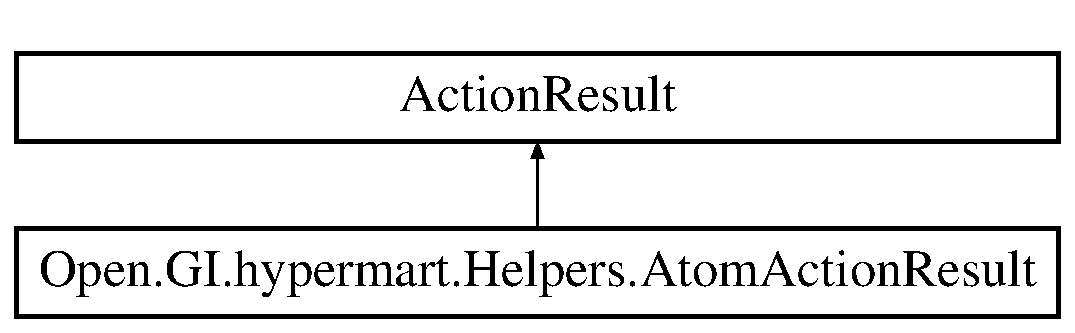
\includegraphics[height=2.000000cm]{class_open_1_1_g_i_1_1hypermart_1_1_helpers_1_1_atom_action_result}
\end{center}
\end{figure}
\subsection*{Public Member Functions}
\begin{DoxyCompactItemize}
\item 
override void \hyperlink{class_open_1_1_g_i_1_1hypermart_1_1_helpers_1_1_atom_action_result_a525b622f00e4c2294a4fedb438273981}{Execute\+Result} (Controller\+Context context)
\begin{DoxyCompactList}\small\item\em Enables processing of the result of an action method by a custom type that inherits from the T\+:\+System.\+Web.\+Mvc.\+Action\+Result class. \end{DoxyCompactList}\end{DoxyCompactItemize}
\subsection*{Properties}
\begin{DoxyCompactItemize}
\item 
Syndication\+Feed \hyperlink{class_open_1_1_g_i_1_1hypermart_1_1_helpers_1_1_atom_action_result_a17a5a951bdf5ed9f8a93f24843e124ca}{Feed}\hspace{0.3cm}{\ttfamily  \mbox{[}get, set\mbox{]}}
\begin{DoxyCompactList}\small\item\em Gets or sets the feed. \end{DoxyCompactList}\end{DoxyCompactItemize}


\subsection{Detailed Description}
Creates an A\+T\+O\+M Result 

\begin{DoxySeeAlso}{See also}
System.\+Web.\+Mvc.\+Action\+Result


\end{DoxySeeAlso}


Definition at line 14 of file Rss\+Action\+Result.\+cs.



\subsection{Member Function Documentation}
\hypertarget{class_open_1_1_g_i_1_1hypermart_1_1_helpers_1_1_atom_action_result_a525b622f00e4c2294a4fedb438273981}{}\index{Open\+::\+G\+I\+::hypermart\+::\+Helpers\+::\+Atom\+Action\+Result@{Open\+::\+G\+I\+::hypermart\+::\+Helpers\+::\+Atom\+Action\+Result}!Execute\+Result@{Execute\+Result}}
\index{Execute\+Result@{Execute\+Result}!Open\+::\+G\+I\+::hypermart\+::\+Helpers\+::\+Atom\+Action\+Result@{Open\+::\+G\+I\+::hypermart\+::\+Helpers\+::\+Atom\+Action\+Result}}
\subsubsection[{Execute\+Result(\+Controller\+Context context)}]{\setlength{\rightskip}{0pt plus 5cm}override void Open.\+G\+I.\+hypermart.\+Helpers.\+Atom\+Action\+Result.\+Execute\+Result (
\begin{DoxyParamCaption}
\item[{Controller\+Context}]{context}
\end{DoxyParamCaption}
)}\label{class_open_1_1_g_i_1_1hypermart_1_1_helpers_1_1_atom_action_result_a525b622f00e4c2294a4fedb438273981}


Enables processing of the result of an action method by a custom type that inherits from the T\+:\+System.\+Web.\+Mvc.\+Action\+Result class. 


\begin{DoxyParams}{Parameters}
{\em context} & The context in which the result is executed. The context information includes the controller, H\+T\+T\+P content, request context, and route data.\\
\hline
\end{DoxyParams}


Definition at line 28 of file Rss\+Action\+Result.\+cs.



\subsection{Property Documentation}
\hypertarget{class_open_1_1_g_i_1_1hypermart_1_1_helpers_1_1_atom_action_result_a17a5a951bdf5ed9f8a93f24843e124ca}{}\index{Open\+::\+G\+I\+::hypermart\+::\+Helpers\+::\+Atom\+Action\+Result@{Open\+::\+G\+I\+::hypermart\+::\+Helpers\+::\+Atom\+Action\+Result}!Feed@{Feed}}
\index{Feed@{Feed}!Open\+::\+G\+I\+::hypermart\+::\+Helpers\+::\+Atom\+Action\+Result@{Open\+::\+G\+I\+::hypermart\+::\+Helpers\+::\+Atom\+Action\+Result}}
\subsubsection[{Feed}]{\setlength{\rightskip}{0pt plus 5cm}Syndication\+Feed Open.\+G\+I.\+hypermart.\+Helpers.\+Atom\+Action\+Result.\+Feed\hspace{0.3cm}{\ttfamily [get]}, {\ttfamily [set]}}\label{class_open_1_1_g_i_1_1hypermart_1_1_helpers_1_1_atom_action_result_a17a5a951bdf5ed9f8a93f24843e124ca}


Gets or sets the feed. 

The feed. 

Definition at line 22 of file Rss\+Action\+Result.\+cs.



The documentation for this class was generated from the following file\+:\begin{DoxyCompactItemize}
\item 
C\+:/\+Projects/\+App-\/\+Utility-\/\+Store/\+Open.\+G\+I.\+hypermart/\+Helpers/\hyperlink{_rss_action_result_8cs}{Rss\+Action\+Result.\+cs}\end{DoxyCompactItemize}

\hypertarget{class_open_1_1_g_i_1_1hypermart_1_1_bundle_config}{}\section{Open.\+G\+I.\+hypermart.\+Bundle\+Config Class Reference}
\label{class_open_1_1_g_i_1_1hypermart_1_1_bundle_config}\index{Open.\+G\+I.\+hypermart.\+Bundle\+Config@{Open.\+G\+I.\+hypermart.\+Bundle\+Config}}


A\+S\+P.\+N\+ET M\+VC Bundle configuration  


\subsection*{Static Public Member Functions}
\begin{DoxyCompactItemize}
\item 
static void \hyperlink{class_open_1_1_g_i_1_1hypermart_1_1_bundle_config_a7b372315a10361265239dc75c616207e}{Register\+Bundles} (Bundle\+Collection bundles)
\begin{DoxyCompactList}\small\item\em Registers the bundles. \end{DoxyCompactList}\end{DoxyCompactItemize}


\subsection{Detailed Description}
A\+S\+P.\+N\+ET M\+VC Bundle configuration 



\subsection{Member Function Documentation}
\hypertarget{class_open_1_1_g_i_1_1hypermart_1_1_bundle_config_a7b372315a10361265239dc75c616207e}{}\label{class_open_1_1_g_i_1_1hypermart_1_1_bundle_config_a7b372315a10361265239dc75c616207e} 
\index{Open\+::\+G\+I\+::hypermart\+::\+Bundle\+Config@{Open\+::\+G\+I\+::hypermart\+::\+Bundle\+Config}!Register\+Bundles@{Register\+Bundles}}
\index{Register\+Bundles@{Register\+Bundles}!Open\+::\+G\+I\+::hypermart\+::\+Bundle\+Config@{Open\+::\+G\+I\+::hypermart\+::\+Bundle\+Config}}
\subsubsection{\texorpdfstring{Register\+Bundles()}{RegisterBundles()}}
{\footnotesize\ttfamily static void Open.\+G\+I.\+hypermart.\+Bundle\+Config.\+Register\+Bundles (\begin{DoxyParamCaption}\item[{Bundle\+Collection}]{bundles }\end{DoxyParamCaption})\hspace{0.3cm}{\ttfamily [static]}}



Registers the bundles. 


\begin{DoxyParams}{Parameters}
{\em bundles} & The bundles.\\
\hline
\end{DoxyParams}


The documentation for this class was generated from the following file\+:\begin{DoxyCompactItemize}
\item 
C\+:/\+Projects/\+App-\/\+Utility-\/\+Store/\+Open.\+G\+I.\+hypermart/\+App\+\_\+\+Start/\hyperlink{_bundle_config_8cs}{Bundle\+Config.\+cs}\end{DoxyCompactItemize}

\hypertarget{class_open_1_1_g_i_1_1hypermart_1_1_models_1_1_category}{}\section{Open.\+G\+I.\+hypermart.\+Models.\+Category Class Reference}
\label{class_open_1_1_g_i_1_1hypermart_1_1_models_1_1_category}\index{Open.\+G\+I.\+hypermart.\+Models.\+Category@{Open.\+G\+I.\+hypermart.\+Models.\+Category}}


 




\subsection{Detailed Description}




The documentation for this class was generated from the following file\+:\begin{DoxyCompactItemize}
\item 
C\+:/\+Projects/\+App-\/\+Utility-\/\+Store/\+Open.\+G\+I.\+hypermart/\+Models/\hyperlink{_category_8cs}{Category.\+cs}\end{DoxyCompactItemize}

\hypertarget{class_open_1_1_g_i_1_1hypermart_1_1_areas_1_1_help_page_1_1_model_descriptions_1_1_collection_model_description}{}\section{Open.\+G\+I.\+hypermart.\+Areas.\+Help\+Page.\+Model\+Descriptions.\+Collection\+Model\+Description Class Reference}
\label{class_open_1_1_g_i_1_1hypermart_1_1_areas_1_1_help_page_1_1_model_descriptions_1_1_collection_model_description}\index{Open.\+G\+I.\+hypermart.\+Areas.\+Help\+Page.\+Model\+Descriptions.\+Collection\+Model\+Description@{Open.\+G\+I.\+hypermart.\+Areas.\+Help\+Page.\+Model\+Descriptions.\+Collection\+Model\+Description}}


 


Inheritance diagram for Open.\+G\+I.\+hypermart.\+Areas.\+Help\+Page.\+Model\+Descriptions.\+Collection\+Model\+Description\+:\begin{figure}[H]
\begin{center}
\leavevmode
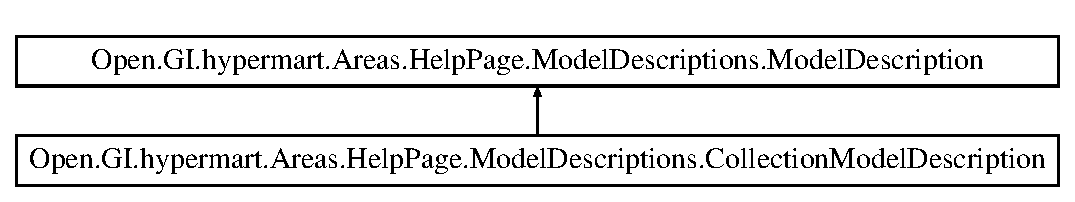
\includegraphics[height=2.000000cm]{class_open_1_1_g_i_1_1hypermart_1_1_areas_1_1_help_page_1_1_model_descriptions_1_1_collection_model_description}
\end{center}
\end{figure}
\subsection*{Properties}
\begin{DoxyCompactItemize}
\item 
\hyperlink{class_open_1_1_g_i_1_1hypermart_1_1_areas_1_1_help_page_1_1_model_descriptions_1_1_model_description}{Model\+Description} \hyperlink{class_open_1_1_g_i_1_1hypermart_1_1_areas_1_1_help_page_1_1_model_descriptions_1_1_collection_model_description_a4049e2a56d1af746b241c4ae2da109ca}{Element\+Description}\hspace{0.3cm}{\ttfamily  \mbox{[}get, set\mbox{]}}
\begin{DoxyCompactList}\small\item\em Gets or sets the element description. \end{DoxyCompactList}\end{DoxyCompactItemize}


\subsection{Detailed Description}


\begin{DoxySeeAlso}{See also}
\hyperlink{class_open_1_1_g_i_1_1hypermart_1_1_areas_1_1_help_page_1_1_model_descriptions_1_1_model_description}{Open.\+G\+I.\+hypermart.\+Areas.\+Help\+Page.\+Model\+Descriptions.\+Model\+Description}


\end{DoxySeeAlso}


\subsection{Property Documentation}
\hypertarget{class_open_1_1_g_i_1_1hypermart_1_1_areas_1_1_help_page_1_1_model_descriptions_1_1_collection_model_description_a4049e2a56d1af746b241c4ae2da109ca}{}\label{class_open_1_1_g_i_1_1hypermart_1_1_areas_1_1_help_page_1_1_model_descriptions_1_1_collection_model_description_a4049e2a56d1af746b241c4ae2da109ca} 
\index{Open\+::\+G\+I\+::hypermart\+::\+Areas\+::\+Help\+Page\+::\+Model\+Descriptions\+::\+Collection\+Model\+Description@{Open\+::\+G\+I\+::hypermart\+::\+Areas\+::\+Help\+Page\+::\+Model\+Descriptions\+::\+Collection\+Model\+Description}!Element\+Description@{Element\+Description}}
\index{Element\+Description@{Element\+Description}!Open\+::\+G\+I\+::hypermart\+::\+Areas\+::\+Help\+Page\+::\+Model\+Descriptions\+::\+Collection\+Model\+Description@{Open\+::\+G\+I\+::hypermart\+::\+Areas\+::\+Help\+Page\+::\+Model\+Descriptions\+::\+Collection\+Model\+Description}}
\subsubsection{\texorpdfstring{Element\+Description}{ElementDescription}}
{\footnotesize\ttfamily \hyperlink{class_open_1_1_g_i_1_1hypermart_1_1_areas_1_1_help_page_1_1_model_descriptions_1_1_model_description}{Model\+Description} Open.\+G\+I.\+hypermart.\+Areas.\+Help\+Page.\+Model\+Descriptions.\+Collection\+Model\+Description.\+Element\+Description\hspace{0.3cm}{\ttfamily [get]}, {\ttfamily [set]}}



Gets or sets the element description. 

The element description. 

The documentation for this class was generated from the following file\+:\begin{DoxyCompactItemize}
\item 
C\+:/\+Projects/\+App-\/\+Utility-\/\+Store/\+Open.\+G\+I.\+hypermart/\+Areas/\+Help\+Page/\+Model\+Descriptions/\hyperlink{_collection_model_description_8cs}{Collection\+Model\+Description.\+cs}\end{DoxyCompactItemize}

\section{Open.\+G\+I.\+hypermart.\+Areas.\+Help\+Page.\+Model\+Descriptions.\+Complex\+Type\+Model\+Description Class Reference}
\label{class_open_1_1_g_i_1_1hypermart_1_1_areas_1_1_help_page_1_1_model_descriptions_1_1_complex_type_model_description}\index{Open.\+G\+I.\+hypermart.\+Areas.\+Help\+Page.\+Model\+Descriptions.\+Complex\+Type\+Model\+Description@{Open.\+G\+I.\+hypermart.\+Areas.\+Help\+Page.\+Model\+Descriptions.\+Complex\+Type\+Model\+Description}}


 


Inheritance diagram for Open.\+G\+I.\+hypermart.\+Areas.\+Help\+Page.\+Model\+Descriptions.\+Complex\+Type\+Model\+Description\+:\begin{figure}[H]
\begin{center}
\leavevmode
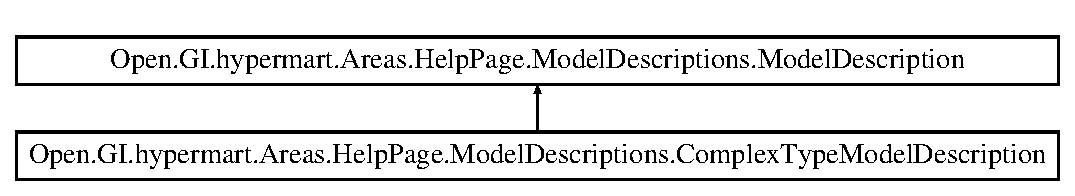
\includegraphics[height=2.000000cm]{class_open_1_1_g_i_1_1hypermart_1_1_areas_1_1_help_page_1_1_model_descriptions_1_1_complex_type_model_description}
\end{center}
\end{figure}
\subsection*{Public Member Functions}
\begin{DoxyCompactItemize}
\item 
\textbf{ Complex\+Type\+Model\+Description} ()
\begin{DoxyCompactList}\small\item\em Initializes a new instance of the \doxyref{Complex\+Type\+Model\+Description}{p.}{class_open_1_1_g_i_1_1hypermart_1_1_areas_1_1_help_page_1_1_model_descriptions_1_1_complex_type_model_description} class. \end{DoxyCompactList}\end{DoxyCompactItemize}
\subsection*{Properties}
\begin{DoxyCompactItemize}
\item 
Collection$<$ \textbf{ Parameter\+Description} $>$ \textbf{ Properties}\hspace{0.3cm}{\ttfamily  [get]}
\begin{DoxyCompactList}\small\item\em Gets the properties. \end{DoxyCompactList}\end{DoxyCompactItemize}


\subsection{Detailed Description}


\begin{DoxySeeAlso}{See also}
\doxyref{Open.\+G\+I.\+hypermart.\+Areas.\+Help\+Page.\+Model\+Descriptions.\+Model\+Description}{p.}{class_open_1_1_g_i_1_1hypermart_1_1_areas_1_1_help_page_1_1_model_descriptions_1_1_model_description}


\end{DoxySeeAlso}


Definition at line 9 of file Complex\+Type\+Model\+Description.\+cs.



\subsection{Constructor \& Destructor Documentation}
\mbox{\label{class_open_1_1_g_i_1_1hypermart_1_1_areas_1_1_help_page_1_1_model_descriptions_1_1_complex_type_model_description_a750b8a599e8e45d091aebfb26edfb3cd}} 
\index{Open\+::\+G\+I\+::hypermart\+::\+Areas\+::\+Help\+Page\+::\+Model\+Descriptions\+::\+Complex\+Type\+Model\+Description@{Open\+::\+G\+I\+::hypermart\+::\+Areas\+::\+Help\+Page\+::\+Model\+Descriptions\+::\+Complex\+Type\+Model\+Description}!Complex\+Type\+Model\+Description@{Complex\+Type\+Model\+Description}}
\index{Complex\+Type\+Model\+Description@{Complex\+Type\+Model\+Description}!Open\+::\+G\+I\+::hypermart\+::\+Areas\+::\+Help\+Page\+::\+Model\+Descriptions\+::\+Complex\+Type\+Model\+Description@{Open\+::\+G\+I\+::hypermart\+::\+Areas\+::\+Help\+Page\+::\+Model\+Descriptions\+::\+Complex\+Type\+Model\+Description}}
\subsubsection{Complex\+Type\+Model\+Description()}
{\footnotesize\ttfamily Open.\+G\+I.\+hypermart.\+Areas.\+Help\+Page.\+Model\+Descriptions.\+Complex\+Type\+Model\+Description.\+Complex\+Type\+Model\+Description (\begin{DoxyParamCaption}{ }\end{DoxyParamCaption})}



Initializes a new instance of the \doxyref{Complex\+Type\+Model\+Description}{p.}{class_open_1_1_g_i_1_1hypermart_1_1_areas_1_1_help_page_1_1_model_descriptions_1_1_complex_type_model_description} class. 



Definition at line 14 of file Complex\+Type\+Model\+Description.\+cs.



\subsection{Property Documentation}
\mbox{\label{class_open_1_1_g_i_1_1hypermart_1_1_areas_1_1_help_page_1_1_model_descriptions_1_1_complex_type_model_description_aef12ede0391a6d743c2f92b1f94d46c2}} 
\index{Open\+::\+G\+I\+::hypermart\+::\+Areas\+::\+Help\+Page\+::\+Model\+Descriptions\+::\+Complex\+Type\+Model\+Description@{Open\+::\+G\+I\+::hypermart\+::\+Areas\+::\+Help\+Page\+::\+Model\+Descriptions\+::\+Complex\+Type\+Model\+Description}!Properties@{Properties}}
\index{Properties@{Properties}!Open\+::\+G\+I\+::hypermart\+::\+Areas\+::\+Help\+Page\+::\+Model\+Descriptions\+::\+Complex\+Type\+Model\+Description@{Open\+::\+G\+I\+::hypermart\+::\+Areas\+::\+Help\+Page\+::\+Model\+Descriptions\+::\+Complex\+Type\+Model\+Description}}
\subsubsection{Properties}
{\footnotesize\ttfamily Collection$<$\textbf{ Parameter\+Description}$>$ Open.\+G\+I.\+hypermart.\+Areas.\+Help\+Page.\+Model\+Descriptions.\+Complex\+Type\+Model\+Description.\+Properties\hspace{0.3cm}{\ttfamily [get]}}



Gets the properties. 

The properties. 

Definition at line 25 of file Complex\+Type\+Model\+Description.\+cs.



The documentation for this class was generated from the following file\+:\begin{DoxyCompactItemize}
\item 
C\+:/\+Projects/\+App-\/\+Utility-\/\+Store/\+Open.\+G\+I.\+hypermart/\+Areas/\+Help\+Page/\+Model\+Descriptions/\textbf{ Complex\+Type\+Model\+Description.\+cs}\end{DoxyCompactItemize}

\hypertarget{class_open_1_1_g_i_1_1hypermart_1_1_areas_1_1_help_page_1_1_model_descriptions_1_1_dictionary_model_description}{}\section{Open.\+G\+I.\+hypermart.\+Areas.\+Help\+Page.\+Model\+Descriptions.\+Dictionary\+Model\+Description Class Reference}
\label{class_open_1_1_g_i_1_1hypermart_1_1_areas_1_1_help_page_1_1_model_descriptions_1_1_dictionary_model_description}\index{Open.\+G\+I.\+hypermart.\+Areas.\+Help\+Page.\+Model\+Descriptions.\+Dictionary\+Model\+Description@{Open.\+G\+I.\+hypermart.\+Areas.\+Help\+Page.\+Model\+Descriptions.\+Dictionary\+Model\+Description}}


 


Inheritance diagram for Open.\+G\+I.\+hypermart.\+Areas.\+Help\+Page.\+Model\+Descriptions.\+Dictionary\+Model\+Description\+:\begin{figure}[H]
\begin{center}
\leavevmode
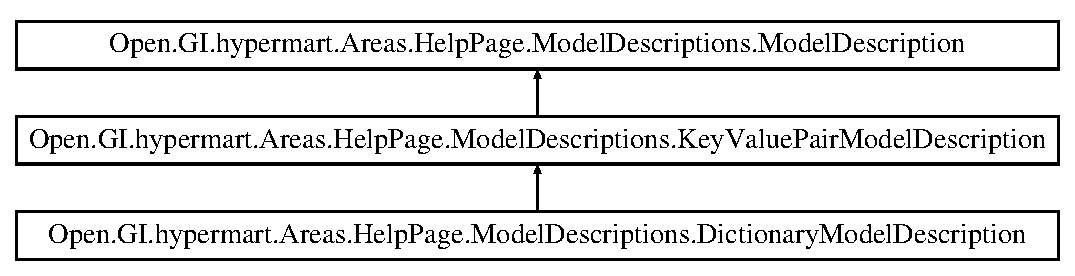
\includegraphics[height=3.000000cm]{class_open_1_1_g_i_1_1hypermart_1_1_areas_1_1_help_page_1_1_model_descriptions_1_1_dictionary_model_description}
\end{center}
\end{figure}
\subsection*{Additional Inherited Members}


\subsection{Detailed Description}


\begin{DoxySeeAlso}{See also}
\hyperlink{class_open_1_1_g_i_1_1hypermart_1_1_areas_1_1_help_page_1_1_model_descriptions_1_1_key_value_pair_model_description}{Open.\+G\+I.\+hypermart.\+Areas.\+Help\+Page.\+Model\+Descriptions.\+Key\+Value\+Pair\+Model\+Description}


\end{DoxySeeAlso}


Definition at line 7 of file Dictionary\+Model\+Description.\+cs.



The documentation for this class was generated from the following file\+:\begin{DoxyCompactItemize}
\item 
C\+:/\+Projects/\+App-\/\+Utility-\/\+Store/\+Open.\+G\+I.\+hypermart/\+Areas/\+Help\+Page/\+Model\+Descriptions/\hyperlink{_dictionary_model_description_8cs}{Dictionary\+Model\+Description.\+cs}\end{DoxyCompactItemize}

\hypertarget{class_open_1_1_g_i_1_1hypermart_1_1_controllers_1_1_download_controller}{}\section{Open.\+G\+I.\+hypermart.\+Controllers.\+Download\+Controller Class Reference}
\label{class_open_1_1_g_i_1_1hypermart_1_1_controllers_1_1_download_controller}\index{Open.\+G\+I.\+hypermart.\+Controllers.\+Download\+Controller@{Open.\+G\+I.\+hypermart.\+Controllers.\+Download\+Controller}}


Controller responsible for serving donwload files to the user.  


Inheritance diagram for Open.\+G\+I.\+hypermart.\+Controllers.\+Download\+Controller\+:\begin{figure}[H]
\begin{center}
\leavevmode
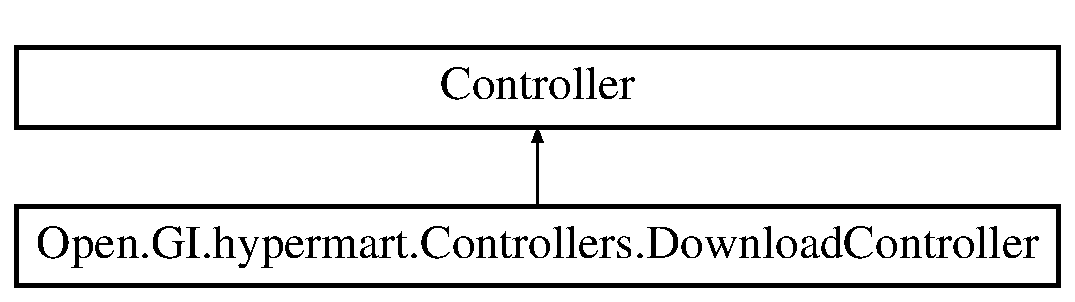
\includegraphics[height=2.000000cm]{class_open_1_1_g_i_1_1hypermart_1_1_controllers_1_1_download_controller}
\end{center}
\end{figure}
\subsection*{Public Member Functions}
\begin{DoxyCompactItemize}
\item 
File\+Result \hyperlink{class_open_1_1_g_i_1_1hypermart_1_1_controllers_1_1_download_controller_a272d3e80defa78e91555596d44891c47}{Download} (int id)
\begin{DoxyCompactList}\small\item\em Downloads the specified identifier. \end{DoxyCompactList}\end{DoxyCompactItemize}


\subsection{Detailed Description}
Controller responsible for serving donwload files to the user. 

\begin{DoxySeeAlso}{See also}
System.\+Web.\+Mvc.\+Controller


\end{DoxySeeAlso}


\subsection{Member Function Documentation}
\hypertarget{class_open_1_1_g_i_1_1hypermart_1_1_controllers_1_1_download_controller_a272d3e80defa78e91555596d44891c47}{}\label{class_open_1_1_g_i_1_1hypermart_1_1_controllers_1_1_download_controller_a272d3e80defa78e91555596d44891c47} 
\index{Open\+::\+G\+I\+::hypermart\+::\+Controllers\+::\+Download\+Controller@{Open\+::\+G\+I\+::hypermart\+::\+Controllers\+::\+Download\+Controller}!Download@{Download}}
\index{Download@{Download}!Open\+::\+G\+I\+::hypermart\+::\+Controllers\+::\+Download\+Controller@{Open\+::\+G\+I\+::hypermart\+::\+Controllers\+::\+Download\+Controller}}
\subsubsection{\texorpdfstring{Download()}{Download()}}
{\footnotesize\ttfamily File\+Result Open.\+G\+I.\+hypermart.\+Controllers.\+Download\+Controller.\+Download (\begin{DoxyParamCaption}\item[{int}]{id }\end{DoxyParamCaption})}



Downloads the specified identifier. 


\begin{DoxyParams}{Parameters}
{\em id} & The identifier.\\
\hline
\end{DoxyParams}
\begin{DoxyReturn}{Returns}

\end{DoxyReturn}

\begin{DoxyExceptions}{Exceptions}
{\em System.\+Web.\+Http\+Exception} & Cannot find file or Cannot find file -\/ can\textquotesingle{}t get remote link. \\
\hline
\end{DoxyExceptions}


The documentation for this class was generated from the following file\+:\begin{DoxyCompactItemize}
\item 
C\+:/\+Projects/\+App-\/\+Utility-\/\+Store/\+Open.\+G\+I.\+hypermart/\+Controllers/\hyperlink{_download_controller_8cs}{Download\+Controller.\+cs}\end{DoxyCompactItemize}

\section{Open.\+G\+I.\+hypermart.\+Areas.\+Help\+Page.\+Model\+Descriptions.\+Enum\+Type\+Model\+Description Class Reference}
\label{class_open_1_1_g_i_1_1hypermart_1_1_areas_1_1_help_page_1_1_model_descriptions_1_1_enum_type_model_description}\index{Open.\+G\+I.\+hypermart.\+Areas.\+Help\+Page.\+Model\+Descriptions.\+Enum\+Type\+Model\+Description@{Open.\+G\+I.\+hypermart.\+Areas.\+Help\+Page.\+Model\+Descriptions.\+Enum\+Type\+Model\+Description}}


 


Inheritance diagram for Open.\+G\+I.\+hypermart.\+Areas.\+Help\+Page.\+Model\+Descriptions.\+Enum\+Type\+Model\+Description\+:\begin{figure}[H]
\begin{center}
\leavevmode
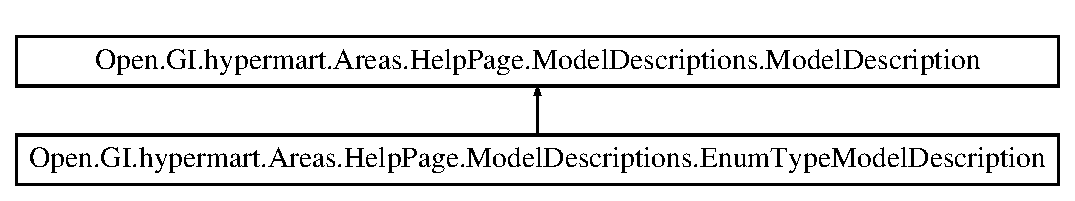
\includegraphics[height=2.000000cm]{class_open_1_1_g_i_1_1hypermart_1_1_areas_1_1_help_page_1_1_model_descriptions_1_1_enum_type_model_description}
\end{center}
\end{figure}
\subsection*{Public Member Functions}
\begin{DoxyCompactItemize}
\item 
\textbf{ Enum\+Type\+Model\+Description} ()
\begin{DoxyCompactList}\small\item\em Initializes a new instance of the \doxyref{Enum\+Type\+Model\+Description}{p.}{class_open_1_1_g_i_1_1hypermart_1_1_areas_1_1_help_page_1_1_model_descriptions_1_1_enum_type_model_description} class. \end{DoxyCompactList}\end{DoxyCompactItemize}
\subsection*{Properties}
\begin{DoxyCompactItemize}
\item 
Collection$<$ \textbf{ Enum\+Value\+Description} $>$ \textbf{ Values}\hspace{0.3cm}{\ttfamily  [get]}
\begin{DoxyCompactList}\small\item\em Gets the values. \end{DoxyCompactList}\end{DoxyCompactItemize}


\subsection{Detailed Description}


\begin{DoxySeeAlso}{See also}
\doxyref{Open.\+G\+I.\+hypermart.\+Areas.\+Help\+Page.\+Model\+Descriptions.\+Model\+Description}{p.}{class_open_1_1_g_i_1_1hypermart_1_1_areas_1_1_help_page_1_1_model_descriptions_1_1_model_description}


\end{DoxySeeAlso}


Definition at line 10 of file Enum\+Type\+Model\+Description.\+cs.



\subsection{Constructor \& Destructor Documentation}
\mbox{\label{class_open_1_1_g_i_1_1hypermart_1_1_areas_1_1_help_page_1_1_model_descriptions_1_1_enum_type_model_description_a77a337dadd9fdcee12869c7385bf51dc}} 
\index{Open\+::\+G\+I\+::hypermart\+::\+Areas\+::\+Help\+Page\+::\+Model\+Descriptions\+::\+Enum\+Type\+Model\+Description@{Open\+::\+G\+I\+::hypermart\+::\+Areas\+::\+Help\+Page\+::\+Model\+Descriptions\+::\+Enum\+Type\+Model\+Description}!Enum\+Type\+Model\+Description@{Enum\+Type\+Model\+Description}}
\index{Enum\+Type\+Model\+Description@{Enum\+Type\+Model\+Description}!Open\+::\+G\+I\+::hypermart\+::\+Areas\+::\+Help\+Page\+::\+Model\+Descriptions\+::\+Enum\+Type\+Model\+Description@{Open\+::\+G\+I\+::hypermart\+::\+Areas\+::\+Help\+Page\+::\+Model\+Descriptions\+::\+Enum\+Type\+Model\+Description}}
\subsubsection{Enum\+Type\+Model\+Description()}
{\footnotesize\ttfamily Open.\+G\+I.\+hypermart.\+Areas.\+Help\+Page.\+Model\+Descriptions.\+Enum\+Type\+Model\+Description.\+Enum\+Type\+Model\+Description (\begin{DoxyParamCaption}{ }\end{DoxyParamCaption})}



Initializes a new instance of the \doxyref{Enum\+Type\+Model\+Description}{p.}{class_open_1_1_g_i_1_1hypermart_1_1_areas_1_1_help_page_1_1_model_descriptions_1_1_enum_type_model_description} class. 



Definition at line 15 of file Enum\+Type\+Model\+Description.\+cs.



\subsection{Property Documentation}
\mbox{\label{class_open_1_1_g_i_1_1hypermart_1_1_areas_1_1_help_page_1_1_model_descriptions_1_1_enum_type_model_description_a7b42c1652865a638dd214ba6a1642819}} 
\index{Open\+::\+G\+I\+::hypermart\+::\+Areas\+::\+Help\+Page\+::\+Model\+Descriptions\+::\+Enum\+Type\+Model\+Description@{Open\+::\+G\+I\+::hypermart\+::\+Areas\+::\+Help\+Page\+::\+Model\+Descriptions\+::\+Enum\+Type\+Model\+Description}!Values@{Values}}
\index{Values@{Values}!Open\+::\+G\+I\+::hypermart\+::\+Areas\+::\+Help\+Page\+::\+Model\+Descriptions\+::\+Enum\+Type\+Model\+Description@{Open\+::\+G\+I\+::hypermart\+::\+Areas\+::\+Help\+Page\+::\+Model\+Descriptions\+::\+Enum\+Type\+Model\+Description}}
\subsubsection{Values}
{\footnotesize\ttfamily Collection$<$\textbf{ Enum\+Value\+Description}$>$ Open.\+G\+I.\+hypermart.\+Areas.\+Help\+Page.\+Model\+Descriptions.\+Enum\+Type\+Model\+Description.\+Values\hspace{0.3cm}{\ttfamily [get]}}



Gets the values. 

The values. 

Definition at line 26 of file Enum\+Type\+Model\+Description.\+cs.



The documentation for this class was generated from the following file\+:\begin{DoxyCompactItemize}
\item 
C\+:/\+Projects/\+App-\/\+Utility-\/\+Store/\+Open.\+G\+I.\+hypermart/\+Areas/\+Help\+Page/\+Model\+Descriptions/\textbf{ Enum\+Type\+Model\+Description.\+cs}\end{DoxyCompactItemize}

\hypertarget{class_open_1_1_g_i_1_1hypermart_1_1_areas_1_1_help_page_1_1_model_descriptions_1_1_enum_value_description}{}\section{Open.\+G\+I.\+hypermart.\+Areas.\+Help\+Page.\+Model\+Descriptions.\+Enum\+Value\+Description Class Reference}
\label{class_open_1_1_g_i_1_1hypermart_1_1_areas_1_1_help_page_1_1_model_descriptions_1_1_enum_value_description}\index{Open.\+G\+I.\+hypermart.\+Areas.\+Help\+Page.\+Model\+Descriptions.\+Enum\+Value\+Description@{Open.\+G\+I.\+hypermart.\+Areas.\+Help\+Page.\+Model\+Descriptions.\+Enum\+Value\+Description}}


 


\subsection*{Properties}
\begin{DoxyCompactItemize}
\item 
string \hyperlink{class_open_1_1_g_i_1_1hypermart_1_1_areas_1_1_help_page_1_1_model_descriptions_1_1_enum_value_description_a8e1e8adc9b367cdc6034e648067585c9}{Documentation}\hspace{0.3cm}{\ttfamily  \mbox{[}get, set\mbox{]}}
\begin{DoxyCompactList}\small\item\em Gets or sets the documentation. \end{DoxyCompactList}\item 
string \hyperlink{class_open_1_1_g_i_1_1hypermart_1_1_areas_1_1_help_page_1_1_model_descriptions_1_1_enum_value_description_a9a7f37f9e6c2a01c41a557b7a8e65d4e}{Name}\hspace{0.3cm}{\ttfamily  \mbox{[}get, set\mbox{]}}
\begin{DoxyCompactList}\small\item\em Gets or sets the name. \end{DoxyCompactList}\item 
string \hyperlink{class_open_1_1_g_i_1_1hypermart_1_1_areas_1_1_help_page_1_1_model_descriptions_1_1_enum_value_description_ab94229a6c9c5afad58abc04d705169f8}{Value}\hspace{0.3cm}{\ttfamily  \mbox{[}get, set\mbox{]}}
\begin{DoxyCompactList}\small\item\em Gets or sets the value. \end{DoxyCompactList}\end{DoxyCompactItemize}


\subsection{Detailed Description}




Definition at line 6 of file Enum\+Value\+Description.\+cs.



\subsection{Property Documentation}
\hypertarget{class_open_1_1_g_i_1_1hypermart_1_1_areas_1_1_help_page_1_1_model_descriptions_1_1_enum_value_description_a8e1e8adc9b367cdc6034e648067585c9}{}\index{Open\+::\+G\+I\+::hypermart\+::\+Areas\+::\+Help\+Page\+::\+Model\+Descriptions\+::\+Enum\+Value\+Description@{Open\+::\+G\+I\+::hypermart\+::\+Areas\+::\+Help\+Page\+::\+Model\+Descriptions\+::\+Enum\+Value\+Description}!Documentation@{Documentation}}
\index{Documentation@{Documentation}!Open\+::\+G\+I\+::hypermart\+::\+Areas\+::\+Help\+Page\+::\+Model\+Descriptions\+::\+Enum\+Value\+Description@{Open\+::\+G\+I\+::hypermart\+::\+Areas\+::\+Help\+Page\+::\+Model\+Descriptions\+::\+Enum\+Value\+Description}}
\subsubsection[{Documentation}]{\setlength{\rightskip}{0pt plus 5cm}string Open.\+G\+I.\+hypermart.\+Areas.\+Help\+Page.\+Model\+Descriptions.\+Enum\+Value\+Description.\+Documentation\hspace{0.3cm}{\ttfamily [get]}, {\ttfamily [set]}}\label{class_open_1_1_g_i_1_1hypermart_1_1_areas_1_1_help_page_1_1_model_descriptions_1_1_enum_value_description_a8e1e8adc9b367cdc6034e648067585c9}


Gets or sets the documentation. 

The documentation. 

Definition at line 14 of file Enum\+Value\+Description.\+cs.

\hypertarget{class_open_1_1_g_i_1_1hypermart_1_1_areas_1_1_help_page_1_1_model_descriptions_1_1_enum_value_description_a9a7f37f9e6c2a01c41a557b7a8e65d4e}{}\index{Open\+::\+G\+I\+::hypermart\+::\+Areas\+::\+Help\+Page\+::\+Model\+Descriptions\+::\+Enum\+Value\+Description@{Open\+::\+G\+I\+::hypermart\+::\+Areas\+::\+Help\+Page\+::\+Model\+Descriptions\+::\+Enum\+Value\+Description}!Name@{Name}}
\index{Name@{Name}!Open\+::\+G\+I\+::hypermart\+::\+Areas\+::\+Help\+Page\+::\+Model\+Descriptions\+::\+Enum\+Value\+Description@{Open\+::\+G\+I\+::hypermart\+::\+Areas\+::\+Help\+Page\+::\+Model\+Descriptions\+::\+Enum\+Value\+Description}}
\subsubsection[{Name}]{\setlength{\rightskip}{0pt plus 5cm}string Open.\+G\+I.\+hypermart.\+Areas.\+Help\+Page.\+Model\+Descriptions.\+Enum\+Value\+Description.\+Name\hspace{0.3cm}{\ttfamily [get]}, {\ttfamily [set]}}\label{class_open_1_1_g_i_1_1hypermart_1_1_areas_1_1_help_page_1_1_model_descriptions_1_1_enum_value_description_a9a7f37f9e6c2a01c41a557b7a8e65d4e}


Gets or sets the name. 

The name. 

Definition at line 22 of file Enum\+Value\+Description.\+cs.

\hypertarget{class_open_1_1_g_i_1_1hypermart_1_1_areas_1_1_help_page_1_1_model_descriptions_1_1_enum_value_description_ab94229a6c9c5afad58abc04d705169f8}{}\index{Open\+::\+G\+I\+::hypermart\+::\+Areas\+::\+Help\+Page\+::\+Model\+Descriptions\+::\+Enum\+Value\+Description@{Open\+::\+G\+I\+::hypermart\+::\+Areas\+::\+Help\+Page\+::\+Model\+Descriptions\+::\+Enum\+Value\+Description}!Value@{Value}}
\index{Value@{Value}!Open\+::\+G\+I\+::hypermart\+::\+Areas\+::\+Help\+Page\+::\+Model\+Descriptions\+::\+Enum\+Value\+Description@{Open\+::\+G\+I\+::hypermart\+::\+Areas\+::\+Help\+Page\+::\+Model\+Descriptions\+::\+Enum\+Value\+Description}}
\subsubsection[{Value}]{\setlength{\rightskip}{0pt plus 5cm}string Open.\+G\+I.\+hypermart.\+Areas.\+Help\+Page.\+Model\+Descriptions.\+Enum\+Value\+Description.\+Value\hspace{0.3cm}{\ttfamily [get]}, {\ttfamily [set]}}\label{class_open_1_1_g_i_1_1hypermart_1_1_areas_1_1_help_page_1_1_model_descriptions_1_1_enum_value_description_ab94229a6c9c5afad58abc04d705169f8}


Gets or sets the value. 

The value. 

Definition at line 30 of file Enum\+Value\+Description.\+cs.



The documentation for this class was generated from the following file\+:\begin{DoxyCompactItemize}
\item 
C\+:/\+Projects/\+App-\/\+Utility-\/\+Store/\+Open.\+G\+I.\+hypermart/\+Areas/\+Help\+Page/\+Model\+Descriptions/\hyperlink{_enum_value_description_8cs}{Enum\+Value\+Description.\+cs}\end{DoxyCompactItemize}

\section{Open.\+G\+I.\+hypermart.\+Models.\+File Class Reference}
\label{class_open_1_1_g_i_1_1hypermart_1_1_models_1_1_file}\index{Open.\+G\+I.\+hypermart.\+Models.\+File@{Open.\+G\+I.\+hypermart.\+Models.\+File}}


Model Class representing a \doxyref{File}{p.}{class_open_1_1_g_i_1_1hypermart_1_1_models_1_1_file}.  


\subsection*{Public Member Functions}
\begin{DoxyCompactItemize}
\item 
\textbf{ File} ()
\begin{DoxyCompactList}\small\item\em Initializes a new instance of the \doxyref{File}{p.}{class_open_1_1_g_i_1_1hypermart_1_1_models_1_1_file} class. \end{DoxyCompactList}\item 
\textbf{ File} ()
\end{DoxyCompactItemize}
\subsection*{Properties}
\begin{DoxyCompactItemize}
\item 
int \textbf{ ID}\hspace{0.3cm}{\ttfamily  [get, set]}
\begin{DoxyCompactList}\small\item\em Gets or sets the identifier. \end{DoxyCompactList}\item 
\textbf{ storage\+Type} \textbf{ Storage\+Type}\hspace{0.3cm}{\ttfamily  [get, set]}
\begin{DoxyCompactList}\small\item\em Gets or sets the type of the storage. \end{DoxyCompactList}\item 
string \textbf{ File\+Name}\hspace{0.3cm}{\ttfamily  [get, set]}
\begin{DoxyCompactList}\small\item\em Gets or sets the name of the file. \end{DoxyCompactList}\item 
byte [$\,$] \textbf{ B\+L\+OB}\hspace{0.3cm}{\ttfamily  [get, set]}
\begin{DoxyCompactList}\small\item\em Gets or sets the B\+L\+OB. \end{DoxyCompactList}\item 
string \textbf{ Link}\hspace{0.3cm}{\ttfamily  [get, set]}
\begin{DoxyCompactList}\small\item\em Gets or sets the link. \end{DoxyCompactList}\item 
string \textbf{ Version}\hspace{0.3cm}{\ttfamily  [get, set]}
\begin{DoxyCompactList}\small\item\em Gets or sets the version. \end{DoxyCompactList}\item 
int \textbf{ Product\+ID}\hspace{0.3cm}{\ttfamily  [get, set]}
\begin{DoxyCompactList}\small\item\em Gets or sets the product identifier. \end{DoxyCompactList}\item 
\textbf{ Product} \textbf{ Product}\hspace{0.3cm}{\ttfamily  [get, set]}
\begin{DoxyCompactList}\small\item\em Gets or sets the product. \end{DoxyCompactList}\item 
virtual I\+Collection$<$ \textbf{ Platform} $>$ \textbf{ Platforms}\hspace{0.3cm}{\ttfamily  [get, set]}
\begin{DoxyCompactList}\small\item\em Gets or sets the platforms. \end{DoxyCompactList}\item 
int \textbf{ Storage\+Type}\hspace{0.3cm}{\ttfamily  [get, set]}
\item 
Nullable$<$ int $>$ \textbf{ Product\+ID}\hspace{0.3cm}{\ttfamily  [get, set]}
\item 
virtual \textbf{ Product} \textbf{ Product}\hspace{0.3cm}{\ttfamily  [get, set]}
\item 
virtual I\+Collection$<$ \textbf{ File\+Platform} $>$ \textbf{ File\+Platforms}\hspace{0.3cm}{\ttfamily  [get, set]}
\end{DoxyCompactItemize}


\subsection{Detailed Description}
Model Class representing a \doxyref{File}{p.}{class_open_1_1_g_i_1_1hypermart_1_1_models_1_1_file}. 



Definition at line 12 of file File.\+cs.



\subsection{Constructor \& Destructor Documentation}
\mbox{\label{class_open_1_1_g_i_1_1hypermart_1_1_models_1_1_file_a6834fcf6e0ea0428dc2decfaa974f8d2}} 
\index{Open\+::\+G\+I\+::hypermart\+::\+Models\+::\+File@{Open\+::\+G\+I\+::hypermart\+::\+Models\+::\+File}!File@{File}}
\index{File@{File}!Open\+::\+G\+I\+::hypermart\+::\+Models\+::\+File@{Open\+::\+G\+I\+::hypermart\+::\+Models\+::\+File}}
\subsubsection{File()\hspace{0.1cm}{\footnotesize\ttfamily [1/2]}}
{\footnotesize\ttfamily Open.\+G\+I.\+hypermart.\+Models.\+File.\+File (\begin{DoxyParamCaption}{ }\end{DoxyParamCaption})}



Initializes a new instance of the \doxyref{File}{p.}{class_open_1_1_g_i_1_1hypermart_1_1_models_1_1_file} class. 



Definition at line 18 of file File.\+cs.

\mbox{\label{class_open_1_1_g_i_1_1hypermart_1_1_models_1_1_file_a6834fcf6e0ea0428dc2decfaa974f8d2}} 
\index{Open\+::\+G\+I\+::hypermart\+::\+Models\+::\+File@{Open\+::\+G\+I\+::hypermart\+::\+Models\+::\+File}!File@{File}}
\index{File@{File}!Open\+::\+G\+I\+::hypermart\+::\+Models\+::\+File@{Open\+::\+G\+I\+::hypermart\+::\+Models\+::\+File}}
\subsubsection{File()\hspace{0.1cm}{\footnotesize\ttfamily [2/2]}}
{\footnotesize\ttfamily Open.\+G\+I.\+hypermart.\+Models.\+File.\+File (\begin{DoxyParamCaption}{ }\end{DoxyParamCaption})}



Definition at line 18 of file File.\+cs.



\subsection{Property Documentation}
\mbox{\label{class_open_1_1_g_i_1_1hypermart_1_1_models_1_1_file_acfdfc6e64338fc14a71994e5d7aa5111}} 
\index{Open\+::\+G\+I\+::hypermart\+::\+Models\+::\+File@{Open\+::\+G\+I\+::hypermart\+::\+Models\+::\+File}!B\+L\+OB@{B\+L\+OB}}
\index{B\+L\+OB@{B\+L\+OB}!Open\+::\+G\+I\+::hypermart\+::\+Models\+::\+File@{Open\+::\+G\+I\+::hypermart\+::\+Models\+::\+File}}
\subsubsection{B\+L\+OB}
{\footnotesize\ttfamily byte [$\,$] Open.\+G\+I.\+hypermart.\+Models.\+File.\+B\+L\+OB\hspace{0.3cm}{\ttfamily [get]}, {\ttfamily [set]}}



Gets or sets the B\+L\+OB. 

The B\+L\+OB. 

Definition at line 53 of file File.\+cs.

\mbox{\label{class_open_1_1_g_i_1_1hypermart_1_1_models_1_1_file_a5675dd150dd5ca0de9bc6755fe6c45ad}} 
\index{Open\+::\+G\+I\+::hypermart\+::\+Models\+::\+File@{Open\+::\+G\+I\+::hypermart\+::\+Models\+::\+File}!File\+Name@{File\+Name}}
\index{File\+Name@{File\+Name}!Open\+::\+G\+I\+::hypermart\+::\+Models\+::\+File@{Open\+::\+G\+I\+::hypermart\+::\+Models\+::\+File}}
\subsubsection{File\+Name}
{\footnotesize\ttfamily string Open.\+G\+I.\+hypermart.\+Models.\+File.\+File\+Name\hspace{0.3cm}{\ttfamily [get]}, {\ttfamily [set]}}



Gets or sets the name of the file. 

The name of the file. 

Definition at line 45 of file File.\+cs.

\mbox{\label{class_open_1_1_g_i_1_1hypermart_1_1_models_1_1_file_ac075b378d09c288deda822c0ea6b854c}} 
\index{Open\+::\+G\+I\+::hypermart\+::\+Models\+::\+File@{Open\+::\+G\+I\+::hypermart\+::\+Models\+::\+File}!File\+Platforms@{File\+Platforms}}
\index{File\+Platforms@{File\+Platforms}!Open\+::\+G\+I\+::hypermart\+::\+Models\+::\+File@{Open\+::\+G\+I\+::hypermart\+::\+Models\+::\+File}}
\subsubsection{File\+Platforms}
{\footnotesize\ttfamily virtual I\+Collection$<$\textbf{ File\+Platform}$>$ Open.\+G\+I.\+hypermart.\+Models.\+File.\+File\+Platforms\hspace{0.3cm}{\ttfamily [get]}, {\ttfamily [set]}}



Definition at line 33 of file File.\+cs.

\mbox{\label{class_open_1_1_g_i_1_1hypermart_1_1_models_1_1_file_ade215e549b777e8f30cfa19ec28cff96}} 
\index{Open\+::\+G\+I\+::hypermart\+::\+Models\+::\+File@{Open\+::\+G\+I\+::hypermart\+::\+Models\+::\+File}!ID@{ID}}
\index{ID@{ID}!Open\+::\+G\+I\+::hypermart\+::\+Models\+::\+File@{Open\+::\+G\+I\+::hypermart\+::\+Models\+::\+File}}
\subsubsection{ID}
{\footnotesize\ttfamily int Open.\+G\+I.\+hypermart.\+Models.\+File.\+ID\hspace{0.3cm}{\ttfamily [get]}, {\ttfamily [set]}}



Gets or sets the identifier. 

The identifier. 

Definition at line 29 of file File.\+cs.

\mbox{\label{class_open_1_1_g_i_1_1hypermart_1_1_models_1_1_file_a47b36d33252b1a1f58bee02a94d11dd5}} 
\index{Open\+::\+G\+I\+::hypermart\+::\+Models\+::\+File@{Open\+::\+G\+I\+::hypermart\+::\+Models\+::\+File}!Link@{Link}}
\index{Link@{Link}!Open\+::\+G\+I\+::hypermart\+::\+Models\+::\+File@{Open\+::\+G\+I\+::hypermart\+::\+Models\+::\+File}}
\subsubsection{Link}
{\footnotesize\ttfamily string Open.\+G\+I.\+hypermart.\+Models.\+File.\+Link\hspace{0.3cm}{\ttfamily [get]}, {\ttfamily [set]}}



Gets or sets the link. 

The link. 

Definition at line 61 of file File.\+cs.

\mbox{\label{class_open_1_1_g_i_1_1hypermart_1_1_models_1_1_file_a7cf38ed851b70df6af9b0606c4d744ed}} 
\index{Open\+::\+G\+I\+::hypermart\+::\+Models\+::\+File@{Open\+::\+G\+I\+::hypermart\+::\+Models\+::\+File}!Platforms@{Platforms}}
\index{Platforms@{Platforms}!Open\+::\+G\+I\+::hypermart\+::\+Models\+::\+File@{Open\+::\+G\+I\+::hypermart\+::\+Models\+::\+File}}
\subsubsection{Platforms}
{\footnotesize\ttfamily virtual I\+Collection$<$\textbf{ Platform}$>$ Open.\+G\+I.\+hypermart.\+Models.\+File.\+Platforms\hspace{0.3cm}{\ttfamily [get]}, {\ttfamily [set]}}



Gets or sets the platforms. 

The platforms. 

Definition at line 95 of file File.\+cs.

\mbox{\label{class_open_1_1_g_i_1_1hypermart_1_1_models_1_1_file_a7a2d45936082be844aa8528b298a2d6a}} 
\index{Open\+::\+G\+I\+::hypermart\+::\+Models\+::\+File@{Open\+::\+G\+I\+::hypermart\+::\+Models\+::\+File}!Product@{Product}}
\index{Product@{Product}!Open\+::\+G\+I\+::hypermart\+::\+Models\+::\+File@{Open\+::\+G\+I\+::hypermart\+::\+Models\+::\+File}}
\subsubsection{Product\hspace{0.1cm}{\footnotesize\ttfamily [1/2]}}
{\footnotesize\ttfamily virtual \textbf{ Product} Open.\+G\+I.\+hypermart.\+Models.\+File.\+Product\hspace{0.3cm}{\ttfamily [get]}, {\ttfamily [set]}}



Definition at line 31 of file File.\+cs.

\mbox{\label{class_open_1_1_g_i_1_1hypermart_1_1_models_1_1_file_a4b8d3f1af1802269e9e06285f9bf81b3}} 
\index{Open\+::\+G\+I\+::hypermart\+::\+Models\+::\+File@{Open\+::\+G\+I\+::hypermart\+::\+Models\+::\+File}!Product@{Product}}
\index{Product@{Product}!Open\+::\+G\+I\+::hypermart\+::\+Models\+::\+File@{Open\+::\+G\+I\+::hypermart\+::\+Models\+::\+File}}
\subsubsection{Product\hspace{0.1cm}{\footnotesize\ttfamily [2/2]}}
{\footnotesize\ttfamily \textbf{ Product} Open.\+G\+I.\+hypermart.\+Models.\+File.\+Product\hspace{0.3cm}{\ttfamily [get]}, {\ttfamily [set]}}



Gets or sets the product. 

The product. 

Definition at line 86 of file File.\+cs.

\mbox{\label{class_open_1_1_g_i_1_1hypermart_1_1_models_1_1_file_ad0b974d38df4491ce90d1d5e884a56a8}} 
\index{Open\+::\+G\+I\+::hypermart\+::\+Models\+::\+File@{Open\+::\+G\+I\+::hypermart\+::\+Models\+::\+File}!Product\+ID@{Product\+ID}}
\index{Product\+ID@{Product\+ID}!Open\+::\+G\+I\+::hypermart\+::\+Models\+::\+File@{Open\+::\+G\+I\+::hypermart\+::\+Models\+::\+File}}
\subsubsection{Product\+ID\hspace{0.1cm}{\footnotesize\ttfamily [1/2]}}
{\footnotesize\ttfamily Nullable$<$int$>$ Open.\+G\+I.\+hypermart.\+Models.\+File.\+Product\+ID\hspace{0.3cm}{\ttfamily [get]}, {\ttfamily [set]}}



Definition at line 29 of file File.\+cs.

\mbox{\label{class_open_1_1_g_i_1_1hypermart_1_1_models_1_1_file_a7f0a3da01808662b23635d9b9b6f6848}} 
\index{Open\+::\+G\+I\+::hypermart\+::\+Models\+::\+File@{Open\+::\+G\+I\+::hypermart\+::\+Models\+::\+File}!Product\+ID@{Product\+ID}}
\index{Product\+ID@{Product\+ID}!Open\+::\+G\+I\+::hypermart\+::\+Models\+::\+File@{Open\+::\+G\+I\+::hypermart\+::\+Models\+::\+File}}
\subsubsection{Product\+ID\hspace{0.1cm}{\footnotesize\ttfamily [2/2]}}
{\footnotesize\ttfamily int Open.\+G\+I.\+hypermart.\+Models.\+File.\+Product\+ID\hspace{0.3cm}{\ttfamily [get]}, {\ttfamily [set]}}



Gets or sets the product identifier. 

The product identifier. 

Definition at line 78 of file File.\+cs.

\mbox{\label{class_open_1_1_g_i_1_1hypermart_1_1_models_1_1_file_ab4ac8af085696918a7a4e1765639066d}} 
\index{Open\+::\+G\+I\+::hypermart\+::\+Models\+::\+File@{Open\+::\+G\+I\+::hypermart\+::\+Models\+::\+File}!Storage\+Type@{Storage\+Type}}
\index{Storage\+Type@{Storage\+Type}!Open\+::\+G\+I\+::hypermart\+::\+Models\+::\+File@{Open\+::\+G\+I\+::hypermart\+::\+Models\+::\+File}}
\subsubsection{Storage\+Type\hspace{0.1cm}{\footnotesize\ttfamily [1/2]}}
{\footnotesize\ttfamily int Open.\+G\+I.\+hypermart.\+Models.\+File.\+Storage\+Type\hspace{0.3cm}{\ttfamily [get]}, {\ttfamily [set]}}



Definition at line 24 of file File.\+cs.

\mbox{\label{class_open_1_1_g_i_1_1hypermart_1_1_models_1_1_file_a4d6910e1f3277beb5b50309e8139a356}} 
\index{Open\+::\+G\+I\+::hypermart\+::\+Models\+::\+File@{Open\+::\+G\+I\+::hypermart\+::\+Models\+::\+File}!Storage\+Type@{Storage\+Type}}
\index{Storage\+Type@{Storage\+Type}!Open\+::\+G\+I\+::hypermart\+::\+Models\+::\+File@{Open\+::\+G\+I\+::hypermart\+::\+Models\+::\+File}}
\subsubsection{Storage\+Type\hspace{0.1cm}{\footnotesize\ttfamily [2/2]}}
{\footnotesize\ttfamily \textbf{ storage\+Type} Open.\+G\+I.\+hypermart.\+Models.\+File.\+Storage\+Type\hspace{0.3cm}{\ttfamily [get]}, {\ttfamily [set]}}



Gets or sets the type of the storage. 

The type of the storage. 

Definition at line 37 of file File.\+cs.

\mbox{\label{class_open_1_1_g_i_1_1hypermart_1_1_models_1_1_file_a59b1cbe55394fce55d55200ea7e55cae}} 
\index{Open\+::\+G\+I\+::hypermart\+::\+Models\+::\+File@{Open\+::\+G\+I\+::hypermart\+::\+Models\+::\+File}!Version@{Version}}
\index{Version@{Version}!Open\+::\+G\+I\+::hypermart\+::\+Models\+::\+File@{Open\+::\+G\+I\+::hypermart\+::\+Models\+::\+File}}
\subsubsection{Version}
{\footnotesize\ttfamily string Open.\+G\+I.\+hypermart.\+Models.\+File.\+Version\hspace{0.3cm}{\ttfamily [get]}, {\ttfamily [set]}}



Gets or sets the version. 

The version. 

Definition at line 70 of file File.\+cs.



The documentation for this class was generated from the following file\+:\begin{DoxyCompactItemize}
\item 
C\+:/\+Projects/\+App-\/\+Utility-\/\+Store/\+Open.\+G\+I.\+hypermart/\+Models/\textbf{ File.\+cs}\end{DoxyCompactItemize}

\hypertarget{class_open_1_1_g_i_1_1hypermart_1_1_data_transformation_objects_1_1_file_d_t_o}{}\section{Open.\+G\+I.\+hypermart.\+Data\+Transformation\+Objects.\+File\+D\+TO Class Reference}
\label{class_open_1_1_g_i_1_1hypermart_1_1_data_transformation_objects_1_1_file_d_t_o}\index{Open.\+G\+I.\+hypermart.\+Data\+Transformation\+Objects.\+File\+D\+TO@{Open.\+G\+I.\+hypermart.\+Data\+Transformation\+Objects.\+File\+D\+TO}}


 


\subsection*{Public Member Functions}
\begin{DoxyCompactItemize}
\item 
\hyperlink{class_open_1_1_g_i_1_1hypermart_1_1_data_transformation_objects_1_1_file_d_t_o_ae0da87388dbf076d2aa151cce63c81a8}{File\+D\+TO} ()
\begin{DoxyCompactList}\small\item\em Initializes a new instance of the \hyperlink{class_open_1_1_g_i_1_1hypermart_1_1_data_transformation_objects_1_1_file_d_t_o}{File\+D\+TO} class. \end{DoxyCompactList}\item 
\hyperlink{class_open_1_1_g_i_1_1hypermart_1_1_data_transformation_objects_1_1_file_d_t_o_add1a3ae47dca46ed24d3d8dda310a3a2}{File\+D\+TO} (\hyperlink{class_open_1_1_g_i_1_1hypermart_1_1_models_1_1_file}{File} \hyperlink{class_open_1_1_g_i_1_1hypermart_1_1_models_1_1_file}{File})
\begin{DoxyCompactList}\small\item\em Initializes a new instance of the \hyperlink{class_open_1_1_g_i_1_1hypermart_1_1_data_transformation_objects_1_1_file_d_t_o}{File\+D\+TO} class. \end{DoxyCompactList}\end{DoxyCompactItemize}
\subsection*{Properties}
\begin{DoxyCompactItemize}
\item 
int \hyperlink{class_open_1_1_g_i_1_1hypermart_1_1_data_transformation_objects_1_1_file_d_t_o_ab187e7f070650067d055de8f707e1eed}{ID}\hspace{0.3cm}{\ttfamily  \mbox{[}get, set\mbox{]}}
\begin{DoxyCompactList}\small\item\em Gets or sets the identifier. \end{DoxyCompactList}\item 
\hyperlink{namespace_open_1_1_g_i_1_1hypermart_1_1_models_a21c5ffa7da75ad8a6d2b04798113f9db}{storage\+Type} \hyperlink{class_open_1_1_g_i_1_1hypermart_1_1_data_transformation_objects_1_1_file_d_t_o_a4563713ee116eb1163eaac1f242b395f}{Storage\+Type}\hspace{0.3cm}{\ttfamily  \mbox{[}get, set\mbox{]}}
\begin{DoxyCompactList}\small\item\em Gets or sets the type of the storage. \end{DoxyCompactList}\item 
string \hyperlink{class_open_1_1_g_i_1_1hypermart_1_1_data_transformation_objects_1_1_file_d_t_o_a55fb34aacab9513037108ff3f1d287a8}{File\+Name}\hspace{0.3cm}{\ttfamily  \mbox{[}get, set\mbox{]}}
\begin{DoxyCompactList}\small\item\em Gets or sets the name of the file. \end{DoxyCompactList}\item 
byte \mbox{[}$\,$\mbox{]} \hyperlink{class_open_1_1_g_i_1_1hypermart_1_1_data_transformation_objects_1_1_file_d_t_o_af2ebb686a878cb8342e76648d048f19a}{B\+L\+OB}\hspace{0.3cm}{\ttfamily  \mbox{[}get, set\mbox{]}}
\begin{DoxyCompactList}\small\item\em Gets or sets the B\+L\+OB. \end{DoxyCompactList}\item 
string \hyperlink{class_open_1_1_g_i_1_1hypermart_1_1_data_transformation_objects_1_1_file_d_t_o_af58091e5ba2e9fde7db92f08dc4d3a41}{Link}\hspace{0.3cm}{\ttfamily  \mbox{[}get, set\mbox{]}}
\begin{DoxyCompactList}\small\item\em Gets or sets the link. \end{DoxyCompactList}\item 
string \hyperlink{class_open_1_1_g_i_1_1hypermart_1_1_data_transformation_objects_1_1_file_d_t_o_ac55a6e7062078277eed54e42b7c29d73}{Version}\hspace{0.3cm}{\ttfamily  \mbox{[}get, set\mbox{]}}
\begin{DoxyCompactList}\small\item\em Gets or sets the version. \end{DoxyCompactList}\item 
int \hyperlink{class_open_1_1_g_i_1_1hypermart_1_1_data_transformation_objects_1_1_file_d_t_o_abd8d9083fbb95dac1e2781f2a8d4f8e9}{Product\+ID}\hspace{0.3cm}{\ttfamily  \mbox{[}get, set\mbox{]}}
\begin{DoxyCompactList}\small\item\em Gets or sets the product identifier. \end{DoxyCompactList}\item 
virtual \hyperlink{class_open_1_1_g_i_1_1hypermart_1_1_models_1_1_product}{Product} \hyperlink{class_open_1_1_g_i_1_1hypermart_1_1_data_transformation_objects_1_1_file_d_t_o_aa587dd986d4c6d62d8bf5520d3a48e79}{Product}\hspace{0.3cm}{\ttfamily  \mbox{[}get, set\mbox{]}}
\begin{DoxyCompactList}\small\item\em Gets or sets the product. \end{DoxyCompactList}\item 
virtual I\+Collection$<$ \hyperlink{class_open_1_1_g_i_1_1hypermart_1_1_models_1_1_platform}{Platform} $>$ \hyperlink{class_open_1_1_g_i_1_1hypermart_1_1_data_transformation_objects_1_1_file_d_t_o_a784824c36cab74d3bc03a8ae55d9a62a}{Platforms}\hspace{0.3cm}{\ttfamily  \mbox{[}get, set\mbox{]}}
\begin{DoxyCompactList}\small\item\em Gets or sets the platforms. \end{DoxyCompactList}\end{DoxyCompactItemize}


\subsection{Detailed Description}




\subsection{Constructor \& Destructor Documentation}
\hypertarget{class_open_1_1_g_i_1_1hypermart_1_1_data_transformation_objects_1_1_file_d_t_o_ae0da87388dbf076d2aa151cce63c81a8}{}\label{class_open_1_1_g_i_1_1hypermart_1_1_data_transformation_objects_1_1_file_d_t_o_ae0da87388dbf076d2aa151cce63c81a8} 
\index{Open\+::\+G\+I\+::hypermart\+::\+Data\+Transformation\+Objects\+::\+File\+D\+TO@{Open\+::\+G\+I\+::hypermart\+::\+Data\+Transformation\+Objects\+::\+File\+D\+TO}!File\+D\+TO@{File\+D\+TO}}
\index{File\+D\+TO@{File\+D\+TO}!Open\+::\+G\+I\+::hypermart\+::\+Data\+Transformation\+Objects\+::\+File\+D\+TO@{Open\+::\+G\+I\+::hypermart\+::\+Data\+Transformation\+Objects\+::\+File\+D\+TO}}
\subsubsection{\texorpdfstring{File\+D\+T\+O()}{FileDTO()}\hspace{0.1cm}{\footnotesize\ttfamily [1/2]}}
{\footnotesize\ttfamily Open.\+G\+I.\+hypermart.\+Data\+Transformation\+Objects.\+File\+D\+T\+O.\+File\+D\+TO (\begin{DoxyParamCaption}{ }\end{DoxyParamCaption})}



Initializes a new instance of the \hyperlink{class_open_1_1_g_i_1_1hypermart_1_1_data_transformation_objects_1_1_file_d_t_o}{File\+D\+TO} class. 

\hypertarget{class_open_1_1_g_i_1_1hypermart_1_1_data_transformation_objects_1_1_file_d_t_o_add1a3ae47dca46ed24d3d8dda310a3a2}{}\label{class_open_1_1_g_i_1_1hypermart_1_1_data_transformation_objects_1_1_file_d_t_o_add1a3ae47dca46ed24d3d8dda310a3a2} 
\index{Open\+::\+G\+I\+::hypermart\+::\+Data\+Transformation\+Objects\+::\+File\+D\+TO@{Open\+::\+G\+I\+::hypermart\+::\+Data\+Transformation\+Objects\+::\+File\+D\+TO}!File\+D\+TO@{File\+D\+TO}}
\index{File\+D\+TO@{File\+D\+TO}!Open\+::\+G\+I\+::hypermart\+::\+Data\+Transformation\+Objects\+::\+File\+D\+TO@{Open\+::\+G\+I\+::hypermart\+::\+Data\+Transformation\+Objects\+::\+File\+D\+TO}}
\subsubsection{\texorpdfstring{File\+D\+T\+O()}{FileDTO()}\hspace{0.1cm}{\footnotesize\ttfamily [2/2]}}
{\footnotesize\ttfamily Open.\+G\+I.\+hypermart.\+Data\+Transformation\+Objects.\+File\+D\+T\+O.\+File\+D\+TO (\begin{DoxyParamCaption}\item[{\hyperlink{class_open_1_1_g_i_1_1hypermart_1_1_models_1_1_file}{File}}]{File }\end{DoxyParamCaption})}



Initializes a new instance of the \hyperlink{class_open_1_1_g_i_1_1hypermart_1_1_data_transformation_objects_1_1_file_d_t_o}{File\+D\+TO} class. 


\begin{DoxyParams}{Parameters}
{\em File} & The file.\\
\hline
\end{DoxyParams}


\subsection{Property Documentation}
\hypertarget{class_open_1_1_g_i_1_1hypermart_1_1_data_transformation_objects_1_1_file_d_t_o_af2ebb686a878cb8342e76648d048f19a}{}\label{class_open_1_1_g_i_1_1hypermart_1_1_data_transformation_objects_1_1_file_d_t_o_af2ebb686a878cb8342e76648d048f19a} 
\index{Open\+::\+G\+I\+::hypermart\+::\+Data\+Transformation\+Objects\+::\+File\+D\+TO@{Open\+::\+G\+I\+::hypermart\+::\+Data\+Transformation\+Objects\+::\+File\+D\+TO}!B\+L\+OB@{B\+L\+OB}}
\index{B\+L\+OB@{B\+L\+OB}!Open\+::\+G\+I\+::hypermart\+::\+Data\+Transformation\+Objects\+::\+File\+D\+TO@{Open\+::\+G\+I\+::hypermart\+::\+Data\+Transformation\+Objects\+::\+File\+D\+TO}}
\subsubsection{\texorpdfstring{B\+L\+OB}{BLOB}}
{\footnotesize\ttfamily byte \mbox{[}$\,$\mbox{]} Open.\+G\+I.\+hypermart.\+Data\+Transformation\+Objects.\+File\+D\+T\+O.\+B\+L\+OB\hspace{0.3cm}{\ttfamily [get]}, {\ttfamily [set]}}



Gets or sets the B\+L\+OB. 

The B\+L\+OB. \hypertarget{class_open_1_1_g_i_1_1hypermart_1_1_data_transformation_objects_1_1_file_d_t_o_a55fb34aacab9513037108ff3f1d287a8}{}\label{class_open_1_1_g_i_1_1hypermart_1_1_data_transformation_objects_1_1_file_d_t_o_a55fb34aacab9513037108ff3f1d287a8} 
\index{Open\+::\+G\+I\+::hypermart\+::\+Data\+Transformation\+Objects\+::\+File\+D\+TO@{Open\+::\+G\+I\+::hypermart\+::\+Data\+Transformation\+Objects\+::\+File\+D\+TO}!File\+Name@{File\+Name}}
\index{File\+Name@{File\+Name}!Open\+::\+G\+I\+::hypermart\+::\+Data\+Transformation\+Objects\+::\+File\+D\+TO@{Open\+::\+G\+I\+::hypermart\+::\+Data\+Transformation\+Objects\+::\+File\+D\+TO}}
\subsubsection{\texorpdfstring{File\+Name}{FileName}}
{\footnotesize\ttfamily string Open.\+G\+I.\+hypermart.\+Data\+Transformation\+Objects.\+File\+D\+T\+O.\+File\+Name\hspace{0.3cm}{\ttfamily [get]}, {\ttfamily [set]}}



Gets or sets the name of the file. 

The name of the file. \hypertarget{class_open_1_1_g_i_1_1hypermart_1_1_data_transformation_objects_1_1_file_d_t_o_ab187e7f070650067d055de8f707e1eed}{}\label{class_open_1_1_g_i_1_1hypermart_1_1_data_transformation_objects_1_1_file_d_t_o_ab187e7f070650067d055de8f707e1eed} 
\index{Open\+::\+G\+I\+::hypermart\+::\+Data\+Transformation\+Objects\+::\+File\+D\+TO@{Open\+::\+G\+I\+::hypermart\+::\+Data\+Transformation\+Objects\+::\+File\+D\+TO}!ID@{ID}}
\index{ID@{ID}!Open\+::\+G\+I\+::hypermart\+::\+Data\+Transformation\+Objects\+::\+File\+D\+TO@{Open\+::\+G\+I\+::hypermart\+::\+Data\+Transformation\+Objects\+::\+File\+D\+TO}}
\subsubsection{\texorpdfstring{ID}{ID}}
{\footnotesize\ttfamily int Open.\+G\+I.\+hypermart.\+Data\+Transformation\+Objects.\+File\+D\+T\+O.\+ID\hspace{0.3cm}{\ttfamily [get]}, {\ttfamily [set]}}



Gets or sets the identifier. 

The identifier. \hypertarget{class_open_1_1_g_i_1_1hypermart_1_1_data_transformation_objects_1_1_file_d_t_o_af58091e5ba2e9fde7db92f08dc4d3a41}{}\label{class_open_1_1_g_i_1_1hypermart_1_1_data_transformation_objects_1_1_file_d_t_o_af58091e5ba2e9fde7db92f08dc4d3a41} 
\index{Open\+::\+G\+I\+::hypermart\+::\+Data\+Transformation\+Objects\+::\+File\+D\+TO@{Open\+::\+G\+I\+::hypermart\+::\+Data\+Transformation\+Objects\+::\+File\+D\+TO}!Link@{Link}}
\index{Link@{Link}!Open\+::\+G\+I\+::hypermart\+::\+Data\+Transformation\+Objects\+::\+File\+D\+TO@{Open\+::\+G\+I\+::hypermart\+::\+Data\+Transformation\+Objects\+::\+File\+D\+TO}}
\subsubsection{\texorpdfstring{Link}{Link}}
{\footnotesize\ttfamily string Open.\+G\+I.\+hypermart.\+Data\+Transformation\+Objects.\+File\+D\+T\+O.\+Link\hspace{0.3cm}{\ttfamily [get]}, {\ttfamily [set]}}



Gets or sets the link. 

The link. \hypertarget{class_open_1_1_g_i_1_1hypermart_1_1_data_transformation_objects_1_1_file_d_t_o_a784824c36cab74d3bc03a8ae55d9a62a}{}\label{class_open_1_1_g_i_1_1hypermart_1_1_data_transformation_objects_1_1_file_d_t_o_a784824c36cab74d3bc03a8ae55d9a62a} 
\index{Open\+::\+G\+I\+::hypermart\+::\+Data\+Transformation\+Objects\+::\+File\+D\+TO@{Open\+::\+G\+I\+::hypermart\+::\+Data\+Transformation\+Objects\+::\+File\+D\+TO}!Platforms@{Platforms}}
\index{Platforms@{Platforms}!Open\+::\+G\+I\+::hypermart\+::\+Data\+Transformation\+Objects\+::\+File\+D\+TO@{Open\+::\+G\+I\+::hypermart\+::\+Data\+Transformation\+Objects\+::\+File\+D\+TO}}
\subsubsection{\texorpdfstring{Platforms}{Platforms}}
{\footnotesize\ttfamily virtual I\+Collection$<$\hyperlink{class_open_1_1_g_i_1_1hypermart_1_1_models_1_1_platform}{Platform}$>$ Open.\+G\+I.\+hypermart.\+Data\+Transformation\+Objects.\+File\+D\+T\+O.\+Platforms\hspace{0.3cm}{\ttfamily [get]}, {\ttfamily [set]}}



Gets or sets the platforms. 

The platforms. \hypertarget{class_open_1_1_g_i_1_1hypermart_1_1_data_transformation_objects_1_1_file_d_t_o_aa587dd986d4c6d62d8bf5520d3a48e79}{}\label{class_open_1_1_g_i_1_1hypermart_1_1_data_transformation_objects_1_1_file_d_t_o_aa587dd986d4c6d62d8bf5520d3a48e79} 
\index{Open\+::\+G\+I\+::hypermart\+::\+Data\+Transformation\+Objects\+::\+File\+D\+TO@{Open\+::\+G\+I\+::hypermart\+::\+Data\+Transformation\+Objects\+::\+File\+D\+TO}!Product@{Product}}
\index{Product@{Product}!Open\+::\+G\+I\+::hypermart\+::\+Data\+Transformation\+Objects\+::\+File\+D\+TO@{Open\+::\+G\+I\+::hypermart\+::\+Data\+Transformation\+Objects\+::\+File\+D\+TO}}
\subsubsection{\texorpdfstring{Product}{Product}}
{\footnotesize\ttfamily virtual \hyperlink{class_open_1_1_g_i_1_1hypermart_1_1_models_1_1_product}{Product} Open.\+G\+I.\+hypermart.\+Data\+Transformation\+Objects.\+File\+D\+T\+O.\+Product\hspace{0.3cm}{\ttfamily [get]}, {\ttfamily [set]}}



Gets or sets the product. 

The product. \hypertarget{class_open_1_1_g_i_1_1hypermart_1_1_data_transformation_objects_1_1_file_d_t_o_abd8d9083fbb95dac1e2781f2a8d4f8e9}{}\label{class_open_1_1_g_i_1_1hypermart_1_1_data_transformation_objects_1_1_file_d_t_o_abd8d9083fbb95dac1e2781f2a8d4f8e9} 
\index{Open\+::\+G\+I\+::hypermart\+::\+Data\+Transformation\+Objects\+::\+File\+D\+TO@{Open\+::\+G\+I\+::hypermart\+::\+Data\+Transformation\+Objects\+::\+File\+D\+TO}!Product\+ID@{Product\+ID}}
\index{Product\+ID@{Product\+ID}!Open\+::\+G\+I\+::hypermart\+::\+Data\+Transformation\+Objects\+::\+File\+D\+TO@{Open\+::\+G\+I\+::hypermart\+::\+Data\+Transformation\+Objects\+::\+File\+D\+TO}}
\subsubsection{\texorpdfstring{Product\+ID}{ProductID}}
{\footnotesize\ttfamily int Open.\+G\+I.\+hypermart.\+Data\+Transformation\+Objects.\+File\+D\+T\+O.\+Product\+ID\hspace{0.3cm}{\ttfamily [get]}, {\ttfamily [set]}}



Gets or sets the product identifier. 

The product identifier. \hypertarget{class_open_1_1_g_i_1_1hypermart_1_1_data_transformation_objects_1_1_file_d_t_o_a4563713ee116eb1163eaac1f242b395f}{}\label{class_open_1_1_g_i_1_1hypermart_1_1_data_transformation_objects_1_1_file_d_t_o_a4563713ee116eb1163eaac1f242b395f} 
\index{Open\+::\+G\+I\+::hypermart\+::\+Data\+Transformation\+Objects\+::\+File\+D\+TO@{Open\+::\+G\+I\+::hypermart\+::\+Data\+Transformation\+Objects\+::\+File\+D\+TO}!Storage\+Type@{Storage\+Type}}
\index{Storage\+Type@{Storage\+Type}!Open\+::\+G\+I\+::hypermart\+::\+Data\+Transformation\+Objects\+::\+File\+D\+TO@{Open\+::\+G\+I\+::hypermart\+::\+Data\+Transformation\+Objects\+::\+File\+D\+TO}}
\subsubsection{\texorpdfstring{Storage\+Type}{StorageType}}
{\footnotesize\ttfamily \hyperlink{namespace_open_1_1_g_i_1_1hypermart_1_1_models_a21c5ffa7da75ad8a6d2b04798113f9db}{storage\+Type} Open.\+G\+I.\+hypermart.\+Data\+Transformation\+Objects.\+File\+D\+T\+O.\+Storage\+Type\hspace{0.3cm}{\ttfamily [get]}, {\ttfamily [set]}}



Gets or sets the type of the storage. 

The type of the storage. \hypertarget{class_open_1_1_g_i_1_1hypermart_1_1_data_transformation_objects_1_1_file_d_t_o_ac55a6e7062078277eed54e42b7c29d73}{}\label{class_open_1_1_g_i_1_1hypermart_1_1_data_transformation_objects_1_1_file_d_t_o_ac55a6e7062078277eed54e42b7c29d73} 
\index{Open\+::\+G\+I\+::hypermart\+::\+Data\+Transformation\+Objects\+::\+File\+D\+TO@{Open\+::\+G\+I\+::hypermart\+::\+Data\+Transformation\+Objects\+::\+File\+D\+TO}!Version@{Version}}
\index{Version@{Version}!Open\+::\+G\+I\+::hypermart\+::\+Data\+Transformation\+Objects\+::\+File\+D\+TO@{Open\+::\+G\+I\+::hypermart\+::\+Data\+Transformation\+Objects\+::\+File\+D\+TO}}
\subsubsection{\texorpdfstring{Version}{Version}}
{\footnotesize\ttfamily string Open.\+G\+I.\+hypermart.\+Data\+Transformation\+Objects.\+File\+D\+T\+O.\+Version\hspace{0.3cm}{\ttfamily [get]}, {\ttfamily [set]}}



Gets or sets the version. 

The version. 

The documentation for this class was generated from the following file\+:\begin{DoxyCompactItemize}
\item 
C\+:/\+Projects/\+App-\/\+Utility-\/\+Store/\+Open.\+G\+I.\+hypermart/\+Docs/\+Data\+Transformation\+Objects/\hyperlink{_file_d_t_o_8cs}{File\+D\+T\+O.\+cs}\end{DoxyCompactItemize}

\hypertarget{class_open_1_1_g_i_1_1hypermart_1_1_models_1_1_file_platform}{}\section{Open.\+G\+I.\+hypermart.\+Models.\+File\+Platform Class Reference}
\label{class_open_1_1_g_i_1_1hypermart_1_1_models_1_1_file_platform}\index{Open.\+G\+I.\+hypermart.\+Models.\+File\+Platform@{Open.\+G\+I.\+hypermart.\+Models.\+File\+Platform}}
\subsection*{Properties}
\begin{DoxyCompactItemize}
\item 
int \hyperlink{class_open_1_1_g_i_1_1hypermart_1_1_models_1_1_file_platform_a6a2b6dbace772016d649b3feb7c65e44}{Files\+\_\+\+I\+D}\hspace{0.3cm}{\ttfamily  \mbox{[}get, set\mbox{]}}
\item 
string \hyperlink{class_open_1_1_g_i_1_1hypermart_1_1_models_1_1_file_platform_afe9e1d6e156cababf5d2123d21556d5f}{Platforms\+\_\+\+I\+D}\hspace{0.3cm}{\ttfamily  \mbox{[}get, set\mbox{]}}
\item 
virtual \hyperlink{class_open_1_1_g_i_1_1hypermart_1_1_models_1_1_platform}{Platform} \hyperlink{class_open_1_1_g_i_1_1hypermart_1_1_models_1_1_file_platform_aeab28cbe72f89ee18f61510d8ea2b7bc}{Platform}\hspace{0.3cm}{\ttfamily  \mbox{[}get, set\mbox{]}}
\item 
virtual \hyperlink{class_open_1_1_g_i_1_1hypermart_1_1_models_1_1_file}{File} \hyperlink{class_open_1_1_g_i_1_1hypermart_1_1_models_1_1_file_platform_aa9fd91411ba71f8dd77bdba062daecd3}{File}\hspace{0.3cm}{\ttfamily  \mbox{[}get, set\mbox{]}}
\end{DoxyCompactItemize}


\subsection{Detailed Description}


Definition at line 15 of file File\+Platform.\+cs.



\subsection{Property Documentation}
\hypertarget{class_open_1_1_g_i_1_1hypermart_1_1_models_1_1_file_platform_aa9fd91411ba71f8dd77bdba062daecd3}{}\index{Open\+::\+G\+I\+::hypermart\+::\+Models\+::\+File\+Platform@{Open\+::\+G\+I\+::hypermart\+::\+Models\+::\+File\+Platform}!File@{File}}
\index{File@{File}!Open\+::\+G\+I\+::hypermart\+::\+Models\+::\+File\+Platform@{Open\+::\+G\+I\+::hypermart\+::\+Models\+::\+File\+Platform}}
\subsubsection[{File}]{\setlength{\rightskip}{0pt plus 5cm}virtual {\bf File} Open.\+G\+I.\+hypermart.\+Models.\+File\+Platform.\+File\hspace{0.3cm}{\ttfamily [get]}, {\ttfamily [set]}}\label{class_open_1_1_g_i_1_1hypermart_1_1_models_1_1_file_platform_aa9fd91411ba71f8dd77bdba062daecd3}


Definition at line 21 of file File\+Platform.\+cs.

\hypertarget{class_open_1_1_g_i_1_1hypermart_1_1_models_1_1_file_platform_a6a2b6dbace772016d649b3feb7c65e44}{}\index{Open\+::\+G\+I\+::hypermart\+::\+Models\+::\+File\+Platform@{Open\+::\+G\+I\+::hypermart\+::\+Models\+::\+File\+Platform}!Files\+\_\+\+I\+D@{Files\+\_\+\+I\+D}}
\index{Files\+\_\+\+I\+D@{Files\+\_\+\+I\+D}!Open\+::\+G\+I\+::hypermart\+::\+Models\+::\+File\+Platform@{Open\+::\+G\+I\+::hypermart\+::\+Models\+::\+File\+Platform}}
\subsubsection[{Files\+\_\+\+I\+D}]{\setlength{\rightskip}{0pt plus 5cm}int Open.\+G\+I.\+hypermart.\+Models.\+File\+Platform.\+Files\+\_\+\+I\+D\hspace{0.3cm}{\ttfamily [get]}, {\ttfamily [set]}}\label{class_open_1_1_g_i_1_1hypermart_1_1_models_1_1_file_platform_a6a2b6dbace772016d649b3feb7c65e44}


Definition at line 17 of file File\+Platform.\+cs.

\hypertarget{class_open_1_1_g_i_1_1hypermart_1_1_models_1_1_file_platform_aeab28cbe72f89ee18f61510d8ea2b7bc}{}\index{Open\+::\+G\+I\+::hypermart\+::\+Models\+::\+File\+Platform@{Open\+::\+G\+I\+::hypermart\+::\+Models\+::\+File\+Platform}!Platform@{Platform}}
\index{Platform@{Platform}!Open\+::\+G\+I\+::hypermart\+::\+Models\+::\+File\+Platform@{Open\+::\+G\+I\+::hypermart\+::\+Models\+::\+File\+Platform}}
\subsubsection[{Platform}]{\setlength{\rightskip}{0pt plus 5cm}virtual {\bf Platform} Open.\+G\+I.\+hypermart.\+Models.\+File\+Platform.\+Platform\hspace{0.3cm}{\ttfamily [get]}, {\ttfamily [set]}}\label{class_open_1_1_g_i_1_1hypermart_1_1_models_1_1_file_platform_aeab28cbe72f89ee18f61510d8ea2b7bc}


Definition at line 20 of file File\+Platform.\+cs.

\hypertarget{class_open_1_1_g_i_1_1hypermart_1_1_models_1_1_file_platform_afe9e1d6e156cababf5d2123d21556d5f}{}\index{Open\+::\+G\+I\+::hypermart\+::\+Models\+::\+File\+Platform@{Open\+::\+G\+I\+::hypermart\+::\+Models\+::\+File\+Platform}!Platforms\+\_\+\+I\+D@{Platforms\+\_\+\+I\+D}}
\index{Platforms\+\_\+\+I\+D@{Platforms\+\_\+\+I\+D}!Open\+::\+G\+I\+::hypermart\+::\+Models\+::\+File\+Platform@{Open\+::\+G\+I\+::hypermart\+::\+Models\+::\+File\+Platform}}
\subsubsection[{Platforms\+\_\+\+I\+D}]{\setlength{\rightskip}{0pt plus 5cm}string Open.\+G\+I.\+hypermart.\+Models.\+File\+Platform.\+Platforms\+\_\+\+I\+D\hspace{0.3cm}{\ttfamily [get]}, {\ttfamily [set]}}\label{class_open_1_1_g_i_1_1hypermart_1_1_models_1_1_file_platform_afe9e1d6e156cababf5d2123d21556d5f}


Definition at line 18 of file File\+Platform.\+cs.



The documentation for this class was generated from the following file\+:\begin{DoxyCompactItemize}
\item 
C\+:/\+Projects/\+App-\/\+Utility-\/\+Store/\+Open.\+G\+I.\+hypermart/\+W\+I\+P/\hyperlink{_file_platform_8cs}{File\+Platform.\+cs}\end{DoxyCompactItemize}

\hypertarget{class_open_1_1_g_i_1_1hypermart_1_1_helpers_1_1_file_share_helper}{}\section{Open.\+G\+I.\+hypermart.\+Helpers.\+File\+Share\+Helper Class Reference}
\label{class_open_1_1_g_i_1_1hypermart_1_1_helpers_1_1_file_share_helper}\index{Open.\+G\+I.\+hypermart.\+Helpers.\+File\+Share\+Helper@{Open.\+G\+I.\+hypermart.\+Helpers.\+File\+Share\+Helper}}


 


\subsection*{Static Public Member Functions}
\begin{DoxyCompactItemize}
\item 
static void \hyperlink{class_open_1_1_g_i_1_1hypermart_1_1_helpers_1_1_file_share_helper_a8e938d7ae2d931ab892c0ebf964ee4d2}{Create\+Folder} (String Folder\+Name)
\begin{DoxyCompactList}\small\item\em Create a Folder -\/ used to create a file System for storing products \end{DoxyCompactList}\item 
static void \hyperlink{class_open_1_1_g_i_1_1hypermart_1_1_helpers_1_1_file_share_helper_af08f7c0abe722a41623b0ae56f78a927}{Create\+Share} (string Folder\+Name, string Share\+Name, string Description)
\begin{DoxyCompactList}\small\item\em Creates the share. \end{DoxyCompactList}\item 
static void \hyperlink{class_open_1_1_g_i_1_1hypermart_1_1_helpers_1_1_file_share_helper_afa333f49f2689e9a64708c27450582ef}{Delete\+Share} (string Folder\+Name)
\begin{DoxyCompactList}\small\item\em Deletes the share. \end{DoxyCompactList}\end{DoxyCompactItemize}


\subsection{Detailed Description}




\subsection{Member Function Documentation}
\hypertarget{class_open_1_1_g_i_1_1hypermart_1_1_helpers_1_1_file_share_helper_a8e938d7ae2d931ab892c0ebf964ee4d2}{}\label{class_open_1_1_g_i_1_1hypermart_1_1_helpers_1_1_file_share_helper_a8e938d7ae2d931ab892c0ebf964ee4d2} 
\index{Open\+::\+G\+I\+::hypermart\+::\+Helpers\+::\+File\+Share\+Helper@{Open\+::\+G\+I\+::hypermart\+::\+Helpers\+::\+File\+Share\+Helper}!Create\+Folder@{Create\+Folder}}
\index{Create\+Folder@{Create\+Folder}!Open\+::\+G\+I\+::hypermart\+::\+Helpers\+::\+File\+Share\+Helper@{Open\+::\+G\+I\+::hypermart\+::\+Helpers\+::\+File\+Share\+Helper}}
\subsubsection{\texorpdfstring{Create\+Folder()}{CreateFolder()}}
{\footnotesize\ttfamily static void Open.\+G\+I.\+hypermart.\+Helpers.\+File\+Share\+Helper.\+Create\+Folder (\begin{DoxyParamCaption}\item[{String}]{Folder\+Name }\end{DoxyParamCaption})\hspace{0.3cm}{\ttfamily [static]}}



Create a Folder -\/ used to create a file System for storing products 


\begin{DoxyParams}{Parameters}
{\em Folder\+Name} & \\
\hline
\end{DoxyParams}
\hypertarget{class_open_1_1_g_i_1_1hypermart_1_1_helpers_1_1_file_share_helper_af08f7c0abe722a41623b0ae56f78a927}{}\label{class_open_1_1_g_i_1_1hypermart_1_1_helpers_1_1_file_share_helper_af08f7c0abe722a41623b0ae56f78a927} 
\index{Open\+::\+G\+I\+::hypermart\+::\+Helpers\+::\+File\+Share\+Helper@{Open\+::\+G\+I\+::hypermart\+::\+Helpers\+::\+File\+Share\+Helper}!Create\+Share@{Create\+Share}}
\index{Create\+Share@{Create\+Share}!Open\+::\+G\+I\+::hypermart\+::\+Helpers\+::\+File\+Share\+Helper@{Open\+::\+G\+I\+::hypermart\+::\+Helpers\+::\+File\+Share\+Helper}}
\subsubsection{\texorpdfstring{Create\+Share()}{CreateShare()}}
{\footnotesize\ttfamily static void Open.\+G\+I.\+hypermart.\+Helpers.\+File\+Share\+Helper.\+Create\+Share (\begin{DoxyParamCaption}\item[{string}]{Folder\+Name,  }\item[{string}]{Share\+Name,  }\item[{string}]{Description }\end{DoxyParamCaption})\hspace{0.3cm}{\ttfamily [static]}}



Creates the share. 


\begin{DoxyParams}{Parameters}
{\em Folder\+Name} & Name of the folder.\\
\hline
{\em Share\+Name} & Name of the share.\\
\hline
{\em Description} & The description.\\
\hline
\end{DoxyParams}

\begin{DoxyExceptions}{Exceptions}
{\em System.\+Exception} & Unable to share directory.\\
\hline
\end{DoxyExceptions}
\hypertarget{class_open_1_1_g_i_1_1hypermart_1_1_helpers_1_1_file_share_helper_afa333f49f2689e9a64708c27450582ef}{}\label{class_open_1_1_g_i_1_1hypermart_1_1_helpers_1_1_file_share_helper_afa333f49f2689e9a64708c27450582ef} 
\index{Open\+::\+G\+I\+::hypermart\+::\+Helpers\+::\+File\+Share\+Helper@{Open\+::\+G\+I\+::hypermart\+::\+Helpers\+::\+File\+Share\+Helper}!Delete\+Share@{Delete\+Share}}
\index{Delete\+Share@{Delete\+Share}!Open\+::\+G\+I\+::hypermart\+::\+Helpers\+::\+File\+Share\+Helper@{Open\+::\+G\+I\+::hypermart\+::\+Helpers\+::\+File\+Share\+Helper}}
\subsubsection{\texorpdfstring{Delete\+Share()}{DeleteShare()}}
{\footnotesize\ttfamily static void Open.\+G\+I.\+hypermart.\+Helpers.\+File\+Share\+Helper.\+Delete\+Share (\begin{DoxyParamCaption}\item[{string}]{Folder\+Name }\end{DoxyParamCaption})\hspace{0.3cm}{\ttfamily [static]}}



Deletes the share. 


\begin{DoxyParams}{Parameters}
{\em Folder\+Name} & Name of the folder.\\
\hline
\end{DoxyParams}


The documentation for this class was generated from the following file\+:\begin{DoxyCompactItemize}
\item 
C\+:/\+Projects/\+App-\/\+Utility-\/\+Store/\+Open.\+G\+I.\+hypermart/\+Helpers/\hyperlink{_file_share_helper_8cs}{File\+Share\+Helper.\+cs}\end{DoxyCompactItemize}

\section{Open.\+G\+I.\+hypermart.\+Filter\+Config Class Reference}
\label{class_open_1_1_g_i_1_1hypermart_1_1_filter_config}\index{Open.\+G\+I.\+hypermart.\+Filter\+Config@{Open.\+G\+I.\+hypermart.\+Filter\+Config}}


Class for filter configuration  


\subsection*{Static Public Member Functions}
\begin{DoxyCompactItemize}
\item 
static void \textbf{ Register\+Global\+Filters} (Global\+Filter\+Collection filters)
\begin{DoxyCompactList}\small\item\em Registers the global filters. \end{DoxyCompactList}\end{DoxyCompactItemize}


\subsection{Detailed Description}
Class for filter configuration 



Definition at line 9 of file Filter\+Config.\+cs.



\subsection{Member Function Documentation}
\mbox{\label{class_open_1_1_g_i_1_1hypermart_1_1_filter_config_a7c2f9e6d0e8157c2942a400ccff8134b}} 
\index{Open\+::\+G\+I\+::hypermart\+::\+Filter\+Config@{Open\+::\+G\+I\+::hypermart\+::\+Filter\+Config}!Register\+Global\+Filters@{Register\+Global\+Filters}}
\index{Register\+Global\+Filters@{Register\+Global\+Filters}!Open\+::\+G\+I\+::hypermart\+::\+Filter\+Config@{Open\+::\+G\+I\+::hypermart\+::\+Filter\+Config}}
\subsubsection{Register\+Global\+Filters()}
{\footnotesize\ttfamily static void Open.\+G\+I.\+hypermart.\+Filter\+Config.\+Register\+Global\+Filters (\begin{DoxyParamCaption}\item[{Global\+Filter\+Collection}]{filters }\end{DoxyParamCaption})\hspace{0.3cm}{\ttfamily [static]}}



Registers the global filters. 


\begin{DoxyParams}{Parameters}
{\em filters} & The filters.\\
\hline
\end{DoxyParams}


Definition at line 15 of file Filter\+Config.\+cs.



The documentation for this class was generated from the following file\+:\begin{DoxyCompactItemize}
\item 
C\+:/\+Projects/\+App-\/\+Utility-\/\+Store/\+Open.\+G\+I.\+hypermart/\+App\+\_\+\+Start/\textbf{ Filter\+Config.\+cs}\end{DoxyCompactItemize}

\section{Open.\+G\+I.\+hypermart.\+Areas.\+Help\+Page.\+Controllers.\+Help\+Controller Class Reference}
\label{class_open_1_1_g_i_1_1hypermart_1_1_areas_1_1_help_page_1_1_controllers_1_1_help_controller}\index{Open.\+G\+I.\+hypermart.\+Areas.\+Help\+Page.\+Controllers.\+Help\+Controller@{Open.\+G\+I.\+hypermart.\+Areas.\+Help\+Page.\+Controllers.\+Help\+Controller}}


The controller that will handle requests for the help page.  


Inheritance diagram for Open.\+G\+I.\+hypermart.\+Areas.\+Help\+Page.\+Controllers.\+Help\+Controller\+:\begin{figure}[H]
\begin{center}
\leavevmode
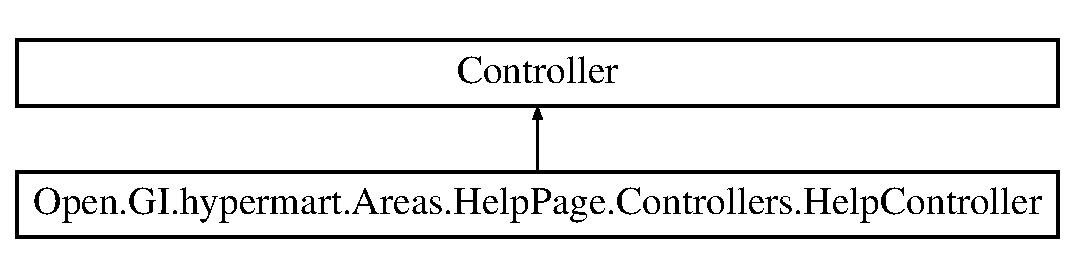
\includegraphics[height=2.000000cm]{class_open_1_1_g_i_1_1hypermart_1_1_areas_1_1_help_page_1_1_controllers_1_1_help_controller}
\end{center}
\end{figure}
\subsection*{Public Member Functions}
\begin{DoxyCompactItemize}
\item 
\textbf{ Help\+Controller} ()
\begin{DoxyCompactList}\small\item\em Initializes a new instance of the \doxyref{Help\+Controller}{p.}{class_open_1_1_g_i_1_1hypermart_1_1_areas_1_1_help_page_1_1_controllers_1_1_help_controller} class. \end{DoxyCompactList}\item 
\textbf{ Help\+Controller} (Http\+Configuration config)
\begin{DoxyCompactList}\small\item\em Initializes a new instance of the \doxyref{Help\+Controller}{p.}{class_open_1_1_g_i_1_1hypermart_1_1_areas_1_1_help_page_1_1_controllers_1_1_help_controller} class. \end{DoxyCompactList}\item 
Action\+Result \textbf{ Index} ()
\begin{DoxyCompactList}\small\item\em Indexes this instance. \end{DoxyCompactList}\item 
Action\+Result \textbf{ Api} (string api\+Id)
\begin{DoxyCompactList}\small\item\em A\+P\+Is the specified A\+PI identifier. \end{DoxyCompactList}\item 
Action\+Result \textbf{ Resource\+Model} (string model\+Name)
\begin{DoxyCompactList}\small\item\em Resources the model. \end{DoxyCompactList}\end{DoxyCompactItemize}
\subsection*{Properties}
\begin{DoxyCompactItemize}
\item 
Http\+Configuration \textbf{ Configuration}\hspace{0.3cm}{\ttfamily  [get]}
\begin{DoxyCompactList}\small\item\em Gets the configuration. \end{DoxyCompactList}\end{DoxyCompactItemize}


\subsection{Detailed Description}
The controller that will handle requests for the help page. 



Definition at line 12 of file Help\+Controller.\+cs.



\subsection{Constructor \& Destructor Documentation}
\mbox{\label{class_open_1_1_g_i_1_1hypermart_1_1_areas_1_1_help_page_1_1_controllers_1_1_help_controller_afa0b9b820c64c6b4f58818ea7a8fbee9}} 
\index{Open\+::\+G\+I\+::hypermart\+::\+Areas\+::\+Help\+Page\+::\+Controllers\+::\+Help\+Controller@{Open\+::\+G\+I\+::hypermart\+::\+Areas\+::\+Help\+Page\+::\+Controllers\+::\+Help\+Controller}!Help\+Controller@{Help\+Controller}}
\index{Help\+Controller@{Help\+Controller}!Open\+::\+G\+I\+::hypermart\+::\+Areas\+::\+Help\+Page\+::\+Controllers\+::\+Help\+Controller@{Open\+::\+G\+I\+::hypermart\+::\+Areas\+::\+Help\+Page\+::\+Controllers\+::\+Help\+Controller}}
\subsubsection{Help\+Controller()\hspace{0.1cm}{\footnotesize\ttfamily [1/2]}}
{\footnotesize\ttfamily Open.\+G\+I.\+hypermart.\+Areas.\+Help\+Page.\+Controllers.\+Help\+Controller.\+Help\+Controller (\begin{DoxyParamCaption}{ }\end{DoxyParamCaption})}



Initializes a new instance of the \doxyref{Help\+Controller}{p.}{class_open_1_1_g_i_1_1hypermart_1_1_areas_1_1_help_page_1_1_controllers_1_1_help_controller} class. 



Definition at line 19 of file Help\+Controller.\+cs.

\mbox{\label{class_open_1_1_g_i_1_1hypermart_1_1_areas_1_1_help_page_1_1_controllers_1_1_help_controller_a5701fb0613147c92bcf47b40636fbb4c}} 
\index{Open\+::\+G\+I\+::hypermart\+::\+Areas\+::\+Help\+Page\+::\+Controllers\+::\+Help\+Controller@{Open\+::\+G\+I\+::hypermart\+::\+Areas\+::\+Help\+Page\+::\+Controllers\+::\+Help\+Controller}!Help\+Controller@{Help\+Controller}}
\index{Help\+Controller@{Help\+Controller}!Open\+::\+G\+I\+::hypermart\+::\+Areas\+::\+Help\+Page\+::\+Controllers\+::\+Help\+Controller@{Open\+::\+G\+I\+::hypermart\+::\+Areas\+::\+Help\+Page\+::\+Controllers\+::\+Help\+Controller}}
\subsubsection{Help\+Controller()\hspace{0.1cm}{\footnotesize\ttfamily [2/2]}}
{\footnotesize\ttfamily Open.\+G\+I.\+hypermart.\+Areas.\+Help\+Page.\+Controllers.\+Help\+Controller.\+Help\+Controller (\begin{DoxyParamCaption}\item[{Http\+Configuration}]{config }\end{DoxyParamCaption})}



Initializes a new instance of the \doxyref{Help\+Controller}{p.}{class_open_1_1_g_i_1_1hypermart_1_1_areas_1_1_help_page_1_1_controllers_1_1_help_controller} class. 


\begin{DoxyParams}{Parameters}
{\em config} & The configuration.\\
\hline
\end{DoxyParams}


Definition at line 28 of file Help\+Controller.\+cs.



\subsection{Member Function Documentation}
\mbox{\label{class_open_1_1_g_i_1_1hypermart_1_1_areas_1_1_help_page_1_1_controllers_1_1_help_controller_a5f4e23a5d390343976a5b04f7a3e9344}} 
\index{Open\+::\+G\+I\+::hypermart\+::\+Areas\+::\+Help\+Page\+::\+Controllers\+::\+Help\+Controller@{Open\+::\+G\+I\+::hypermart\+::\+Areas\+::\+Help\+Page\+::\+Controllers\+::\+Help\+Controller}!Api@{Api}}
\index{Api@{Api}!Open\+::\+G\+I\+::hypermart\+::\+Areas\+::\+Help\+Page\+::\+Controllers\+::\+Help\+Controller@{Open\+::\+G\+I\+::hypermart\+::\+Areas\+::\+Help\+Page\+::\+Controllers\+::\+Help\+Controller}}
\subsubsection{Api()}
{\footnotesize\ttfamily Action\+Result Open.\+G\+I.\+hypermart.\+Areas.\+Help\+Page.\+Controllers.\+Help\+Controller.\+Api (\begin{DoxyParamCaption}\item[{string}]{api\+Id }\end{DoxyParamCaption})}



A\+P\+Is the specified A\+PI identifier. 


\begin{DoxyParams}{Parameters}
{\em api\+Id} & The A\+PI identifier.\\
\hline
\end{DoxyParams}
\begin{DoxyReturn}{Returns}

\end{DoxyReturn}


Definition at line 56 of file Help\+Controller.\+cs.

\mbox{\label{class_open_1_1_g_i_1_1hypermart_1_1_areas_1_1_help_page_1_1_controllers_1_1_help_controller_a4c63414e59364e8ce99be20a5c909da8}} 
\index{Open\+::\+G\+I\+::hypermart\+::\+Areas\+::\+Help\+Page\+::\+Controllers\+::\+Help\+Controller@{Open\+::\+G\+I\+::hypermart\+::\+Areas\+::\+Help\+Page\+::\+Controllers\+::\+Help\+Controller}!Index@{Index}}
\index{Index@{Index}!Open\+::\+G\+I\+::hypermart\+::\+Areas\+::\+Help\+Page\+::\+Controllers\+::\+Help\+Controller@{Open\+::\+G\+I\+::hypermart\+::\+Areas\+::\+Help\+Page\+::\+Controllers\+::\+Help\+Controller}}
\subsubsection{Index()}
{\footnotesize\ttfamily Action\+Result Open.\+G\+I.\+hypermart.\+Areas.\+Help\+Page.\+Controllers.\+Help\+Controller.\+Index (\begin{DoxyParamCaption}{ }\end{DoxyParamCaption})}



Indexes this instance. 

\begin{DoxyReturn}{Returns}

\end{DoxyReturn}


Definition at line 45 of file Help\+Controller.\+cs.

\mbox{\label{class_open_1_1_g_i_1_1hypermart_1_1_areas_1_1_help_page_1_1_controllers_1_1_help_controller_a374c9c2d8d4630c433a397b3ac76c53c}} 
\index{Open\+::\+G\+I\+::hypermart\+::\+Areas\+::\+Help\+Page\+::\+Controllers\+::\+Help\+Controller@{Open\+::\+G\+I\+::hypermart\+::\+Areas\+::\+Help\+Page\+::\+Controllers\+::\+Help\+Controller}!Resource\+Model@{Resource\+Model}}
\index{Resource\+Model@{Resource\+Model}!Open\+::\+G\+I\+::hypermart\+::\+Areas\+::\+Help\+Page\+::\+Controllers\+::\+Help\+Controller@{Open\+::\+G\+I\+::hypermart\+::\+Areas\+::\+Help\+Page\+::\+Controllers\+::\+Help\+Controller}}
\subsubsection{Resource\+Model()}
{\footnotesize\ttfamily Action\+Result Open.\+G\+I.\+hypermart.\+Areas.\+Help\+Page.\+Controllers.\+Help\+Controller.\+Resource\+Model (\begin{DoxyParamCaption}\item[{string}]{model\+Name }\end{DoxyParamCaption})}



Resources the model. 


\begin{DoxyParams}{Parameters}
{\em model\+Name} & Name of the model.\\
\hline
\end{DoxyParams}
\begin{DoxyReturn}{Returns}

\end{DoxyReturn}


Definition at line 75 of file Help\+Controller.\+cs.



\subsection{Property Documentation}
\mbox{\label{class_open_1_1_g_i_1_1hypermart_1_1_areas_1_1_help_page_1_1_controllers_1_1_help_controller_ac1327fb5827701100fa4e1b3566fd752}} 
\index{Open\+::\+G\+I\+::hypermart\+::\+Areas\+::\+Help\+Page\+::\+Controllers\+::\+Help\+Controller@{Open\+::\+G\+I\+::hypermart\+::\+Areas\+::\+Help\+Page\+::\+Controllers\+::\+Help\+Controller}!Configuration@{Configuration}}
\index{Configuration@{Configuration}!Open\+::\+G\+I\+::hypermart\+::\+Areas\+::\+Help\+Page\+::\+Controllers\+::\+Help\+Controller@{Open\+::\+G\+I\+::hypermart\+::\+Areas\+::\+Help\+Page\+::\+Controllers\+::\+Help\+Controller}}
\subsubsection{Configuration}
{\footnotesize\ttfamily Http\+Configuration Open.\+G\+I.\+hypermart.\+Areas.\+Help\+Page.\+Controllers.\+Help\+Controller.\+Configuration\hspace{0.3cm}{\ttfamily [get]}}



Gets the configuration. 

The configuration. 

Definition at line 39 of file Help\+Controller.\+cs.



The documentation for this class was generated from the following file\+:\begin{DoxyCompactItemize}
\item 
C\+:/\+Projects/\+App-\/\+Utility-\/\+Store/\+Open.\+G\+I.\+hypermart/\+Areas/\+Help\+Page/\+Controllers/\textbf{ Help\+Controller.\+cs}\end{DoxyCompactItemize}

\section{Open.\+G\+I.\+hypermart.\+Areas.\+Help\+Page.\+Models.\+Help\+Page\+Api\+Model Class Reference}
\label{class_open_1_1_g_i_1_1hypermart_1_1_areas_1_1_help_page_1_1_models_1_1_help_page_api_model}\index{Open.\+G\+I.\+hypermart.\+Areas.\+Help\+Page.\+Models.\+Help\+Page\+Api\+Model@{Open.\+G\+I.\+hypermart.\+Areas.\+Help\+Page.\+Models.\+Help\+Page\+Api\+Model}}


The model that represents an A\+PI displayed on the help page.  


\subsection*{Public Member Functions}
\begin{DoxyCompactItemize}
\item 
\textbf{ Help\+Page\+Api\+Model} ()
\begin{DoxyCompactList}\small\item\em Initializes a new instance of the \doxyref{Help\+Page\+Api\+Model}{p.}{class_open_1_1_g_i_1_1hypermart_1_1_areas_1_1_help_page_1_1_models_1_1_help_page_api_model} class. \end{DoxyCompactList}\end{DoxyCompactItemize}
\subsection*{Properties}
\begin{DoxyCompactItemize}
\item 
Api\+Description \textbf{ Api\+Description}\hspace{0.3cm}{\ttfamily  [get, set]}
\begin{DoxyCompactList}\small\item\em Gets or sets the \doxyref{Api\+Description}{p.}{class_open_1_1_g_i_1_1hypermart_1_1_areas_1_1_help_page_1_1_models_1_1_help_page_api_model_a80061bc5f25f38dbfbff06705a48372e} that describes the A\+PI. \end{DoxyCompactList}\item 
Collection$<$ \textbf{ Parameter\+Description} $>$ \textbf{ Uri\+Parameters}\hspace{0.3cm}{\ttfamily  [get]}
\begin{DoxyCompactList}\small\item\em Gets or sets the Parameter\+Description collection that describes the U\+RI parameters for the A\+PI. \end{DoxyCompactList}\item 
string \textbf{ Request\+Documentation}\hspace{0.3cm}{\ttfamily  [get, set]}
\begin{DoxyCompactList}\small\item\em Gets or sets the documentation for the request. \end{DoxyCompactList}\item 
\textbf{ Model\+Description} \textbf{ Request\+Model\+Description}\hspace{0.3cm}{\ttfamily  [get, set]}
\begin{DoxyCompactList}\small\item\em Gets or sets the Model\+Description that describes the request body. \end{DoxyCompactList}\item 
I\+List$<$ \textbf{ Parameter\+Description} $>$ \textbf{ Request\+Body\+Parameters}\hspace{0.3cm}{\ttfamily  [get]}
\begin{DoxyCompactList}\small\item\em Gets the request body parameter descriptions. \end{DoxyCompactList}\item 
\textbf{ Model\+Description} \textbf{ Resource\+Description}\hspace{0.3cm}{\ttfamily  [get, set]}
\begin{DoxyCompactList}\small\item\em Gets or sets the Model\+Description that describes the resource. \end{DoxyCompactList}\item 
I\+List$<$ \textbf{ Parameter\+Description} $>$ \textbf{ Resource\+Properties}\hspace{0.3cm}{\ttfamily  [get]}
\begin{DoxyCompactList}\small\item\em Gets the resource property descriptions. \end{DoxyCompactList}\item 
I\+Dictionary$<$ Media\+Type\+Header\+Value, object $>$ \textbf{ Sample\+Requests}\hspace{0.3cm}{\ttfamily  [get]}
\begin{DoxyCompactList}\small\item\em Gets the sample requests associated with the A\+PI. \end{DoxyCompactList}\item 
I\+Dictionary$<$ Media\+Type\+Header\+Value, object $>$ \textbf{ Sample\+Responses}\hspace{0.3cm}{\ttfamily  [get]}
\begin{DoxyCompactList}\small\item\em Gets the sample responses associated with the A\+PI. \end{DoxyCompactList}\item 
Collection$<$ string $>$ \textbf{ Error\+Messages}\hspace{0.3cm}{\ttfamily  [get]}
\begin{DoxyCompactList}\small\item\em Gets the error messages associated with this model. \end{DoxyCompactList}\end{DoxyCompactItemize}


\subsection{Detailed Description}
The model that represents an A\+PI displayed on the help page. 



Definition at line 12 of file Help\+Page\+Api\+Model.\+cs.



\subsection{Constructor \& Destructor Documentation}
\mbox{\label{class_open_1_1_g_i_1_1hypermart_1_1_areas_1_1_help_page_1_1_models_1_1_help_page_api_model_a34aa95dfea87b53bcfac8601fb1f3b93}} 
\index{Open\+::\+G\+I\+::hypermart\+::\+Areas\+::\+Help\+Page\+::\+Models\+::\+Help\+Page\+Api\+Model@{Open\+::\+G\+I\+::hypermart\+::\+Areas\+::\+Help\+Page\+::\+Models\+::\+Help\+Page\+Api\+Model}!Help\+Page\+Api\+Model@{Help\+Page\+Api\+Model}}
\index{Help\+Page\+Api\+Model@{Help\+Page\+Api\+Model}!Open\+::\+G\+I\+::hypermart\+::\+Areas\+::\+Help\+Page\+::\+Models\+::\+Help\+Page\+Api\+Model@{Open\+::\+G\+I\+::hypermart\+::\+Areas\+::\+Help\+Page\+::\+Models\+::\+Help\+Page\+Api\+Model}}
\subsubsection{Help\+Page\+Api\+Model()}
{\footnotesize\ttfamily Open.\+G\+I.\+hypermart.\+Areas.\+Help\+Page.\+Models.\+Help\+Page\+Api\+Model.\+Help\+Page\+Api\+Model (\begin{DoxyParamCaption}{ }\end{DoxyParamCaption})}



Initializes a new instance of the \doxyref{Help\+Page\+Api\+Model}{p.}{class_open_1_1_g_i_1_1hypermart_1_1_areas_1_1_help_page_1_1_models_1_1_help_page_api_model} class. 



Definition at line 17 of file Help\+Page\+Api\+Model.\+cs.



\subsection{Property Documentation}
\mbox{\label{class_open_1_1_g_i_1_1hypermart_1_1_areas_1_1_help_page_1_1_models_1_1_help_page_api_model_a80061bc5f25f38dbfbff06705a48372e}} 
\index{Open\+::\+G\+I\+::hypermart\+::\+Areas\+::\+Help\+Page\+::\+Models\+::\+Help\+Page\+Api\+Model@{Open\+::\+G\+I\+::hypermart\+::\+Areas\+::\+Help\+Page\+::\+Models\+::\+Help\+Page\+Api\+Model}!Api\+Description@{Api\+Description}}
\index{Api\+Description@{Api\+Description}!Open\+::\+G\+I\+::hypermart\+::\+Areas\+::\+Help\+Page\+::\+Models\+::\+Help\+Page\+Api\+Model@{Open\+::\+G\+I\+::hypermart\+::\+Areas\+::\+Help\+Page\+::\+Models\+::\+Help\+Page\+Api\+Model}}
\subsubsection{Api\+Description}
{\footnotesize\ttfamily Api\+Description Open.\+G\+I.\+hypermart.\+Areas.\+Help\+Page.\+Models.\+Help\+Page\+Api\+Model.\+Api\+Description\hspace{0.3cm}{\ttfamily [get]}, {\ttfamily [set]}}



Gets or sets the \doxyref{Api\+Description}{p.}{class_open_1_1_g_i_1_1hypermart_1_1_areas_1_1_help_page_1_1_models_1_1_help_page_api_model_a80061bc5f25f38dbfbff06705a48372e} that describes the A\+PI. 



Definition at line 28 of file Help\+Page\+Api\+Model.\+cs.

\mbox{\label{class_open_1_1_g_i_1_1hypermart_1_1_areas_1_1_help_page_1_1_models_1_1_help_page_api_model_a318df386bf722bfbafab9a6f2812641e}} 
\index{Open\+::\+G\+I\+::hypermart\+::\+Areas\+::\+Help\+Page\+::\+Models\+::\+Help\+Page\+Api\+Model@{Open\+::\+G\+I\+::hypermart\+::\+Areas\+::\+Help\+Page\+::\+Models\+::\+Help\+Page\+Api\+Model}!Error\+Messages@{Error\+Messages}}
\index{Error\+Messages@{Error\+Messages}!Open\+::\+G\+I\+::hypermart\+::\+Areas\+::\+Help\+Page\+::\+Models\+::\+Help\+Page\+Api\+Model@{Open\+::\+G\+I\+::hypermart\+::\+Areas\+::\+Help\+Page\+::\+Models\+::\+Help\+Page\+Api\+Model}}
\subsubsection{Error\+Messages}
{\footnotesize\ttfamily Collection$<$string$>$ Open.\+G\+I.\+hypermart.\+Areas.\+Help\+Page.\+Models.\+Help\+Page\+Api\+Model.\+Error\+Messages\hspace{0.3cm}{\ttfamily [get]}}



Gets the error messages associated with this model. 



Definition at line 85 of file Help\+Page\+Api\+Model.\+cs.

\mbox{\label{class_open_1_1_g_i_1_1hypermart_1_1_areas_1_1_help_page_1_1_models_1_1_help_page_api_model_a6b2ccd725318cec7557237bb25272ac0}} 
\index{Open\+::\+G\+I\+::hypermart\+::\+Areas\+::\+Help\+Page\+::\+Models\+::\+Help\+Page\+Api\+Model@{Open\+::\+G\+I\+::hypermart\+::\+Areas\+::\+Help\+Page\+::\+Models\+::\+Help\+Page\+Api\+Model}!Request\+Body\+Parameters@{Request\+Body\+Parameters}}
\index{Request\+Body\+Parameters@{Request\+Body\+Parameters}!Open\+::\+G\+I\+::hypermart\+::\+Areas\+::\+Help\+Page\+::\+Models\+::\+Help\+Page\+Api\+Model@{Open\+::\+G\+I\+::hypermart\+::\+Areas\+::\+Help\+Page\+::\+Models\+::\+Help\+Page\+Api\+Model}}
\subsubsection{Request\+Body\+Parameters}
{\footnotesize\ttfamily I\+List$<$\textbf{ Parameter\+Description}$>$ Open.\+G\+I.\+hypermart.\+Areas.\+Help\+Page.\+Models.\+Help\+Page\+Api\+Model.\+Request\+Body\+Parameters\hspace{0.3cm}{\ttfamily [get]}}



Gets the request body parameter descriptions. 



Definition at line 49 of file Help\+Page\+Api\+Model.\+cs.

\mbox{\label{class_open_1_1_g_i_1_1hypermart_1_1_areas_1_1_help_page_1_1_models_1_1_help_page_api_model_aa27a2376388763669d59b97fab474a47}} 
\index{Open\+::\+G\+I\+::hypermart\+::\+Areas\+::\+Help\+Page\+::\+Models\+::\+Help\+Page\+Api\+Model@{Open\+::\+G\+I\+::hypermart\+::\+Areas\+::\+Help\+Page\+::\+Models\+::\+Help\+Page\+Api\+Model}!Request\+Documentation@{Request\+Documentation}}
\index{Request\+Documentation@{Request\+Documentation}!Open\+::\+G\+I\+::hypermart\+::\+Areas\+::\+Help\+Page\+::\+Models\+::\+Help\+Page\+Api\+Model@{Open\+::\+G\+I\+::hypermart\+::\+Areas\+::\+Help\+Page\+::\+Models\+::\+Help\+Page\+Api\+Model}}
\subsubsection{Request\+Documentation}
{\footnotesize\ttfamily string Open.\+G\+I.\+hypermart.\+Areas.\+Help\+Page.\+Models.\+Help\+Page\+Api\+Model.\+Request\+Documentation\hspace{0.3cm}{\ttfamily [get]}, {\ttfamily [set]}}



Gets or sets the documentation for the request. 



Definition at line 38 of file Help\+Page\+Api\+Model.\+cs.

\mbox{\label{class_open_1_1_g_i_1_1hypermart_1_1_areas_1_1_help_page_1_1_models_1_1_help_page_api_model_a9922daf50e7226b541b2906b6011947c}} 
\index{Open\+::\+G\+I\+::hypermart\+::\+Areas\+::\+Help\+Page\+::\+Models\+::\+Help\+Page\+Api\+Model@{Open\+::\+G\+I\+::hypermart\+::\+Areas\+::\+Help\+Page\+::\+Models\+::\+Help\+Page\+Api\+Model}!Request\+Model\+Description@{Request\+Model\+Description}}
\index{Request\+Model\+Description@{Request\+Model\+Description}!Open\+::\+G\+I\+::hypermart\+::\+Areas\+::\+Help\+Page\+::\+Models\+::\+Help\+Page\+Api\+Model@{Open\+::\+G\+I\+::hypermart\+::\+Areas\+::\+Help\+Page\+::\+Models\+::\+Help\+Page\+Api\+Model}}
\subsubsection{Request\+Model\+Description}
{\footnotesize\ttfamily \textbf{ Model\+Description} Open.\+G\+I.\+hypermart.\+Areas.\+Help\+Page.\+Models.\+Help\+Page\+Api\+Model.\+Request\+Model\+Description\hspace{0.3cm}{\ttfamily [get]}, {\ttfamily [set]}}



Gets or sets the Model\+Description that describes the request body. 



Definition at line 43 of file Help\+Page\+Api\+Model.\+cs.

\mbox{\label{class_open_1_1_g_i_1_1hypermart_1_1_areas_1_1_help_page_1_1_models_1_1_help_page_api_model_a69f18559e320aecc4dc81f68b8327729}} 
\index{Open\+::\+G\+I\+::hypermart\+::\+Areas\+::\+Help\+Page\+::\+Models\+::\+Help\+Page\+Api\+Model@{Open\+::\+G\+I\+::hypermart\+::\+Areas\+::\+Help\+Page\+::\+Models\+::\+Help\+Page\+Api\+Model}!Resource\+Description@{Resource\+Description}}
\index{Resource\+Description@{Resource\+Description}!Open\+::\+G\+I\+::hypermart\+::\+Areas\+::\+Help\+Page\+::\+Models\+::\+Help\+Page\+Api\+Model@{Open\+::\+G\+I\+::hypermart\+::\+Areas\+::\+Help\+Page\+::\+Models\+::\+Help\+Page\+Api\+Model}}
\subsubsection{Resource\+Description}
{\footnotesize\ttfamily \textbf{ Model\+Description} Open.\+G\+I.\+hypermart.\+Areas.\+Help\+Page.\+Models.\+Help\+Page\+Api\+Model.\+Resource\+Description\hspace{0.3cm}{\ttfamily [get]}, {\ttfamily [set]}}



Gets or sets the Model\+Description that describes the resource. 



Definition at line 59 of file Help\+Page\+Api\+Model.\+cs.

\mbox{\label{class_open_1_1_g_i_1_1hypermart_1_1_areas_1_1_help_page_1_1_models_1_1_help_page_api_model_a1fc678443900b538ee0b4bbd22e9b4d3}} 
\index{Open\+::\+G\+I\+::hypermart\+::\+Areas\+::\+Help\+Page\+::\+Models\+::\+Help\+Page\+Api\+Model@{Open\+::\+G\+I\+::hypermart\+::\+Areas\+::\+Help\+Page\+::\+Models\+::\+Help\+Page\+Api\+Model}!Resource\+Properties@{Resource\+Properties}}
\index{Resource\+Properties@{Resource\+Properties}!Open\+::\+G\+I\+::hypermart\+::\+Areas\+::\+Help\+Page\+::\+Models\+::\+Help\+Page\+Api\+Model@{Open\+::\+G\+I\+::hypermart\+::\+Areas\+::\+Help\+Page\+::\+Models\+::\+Help\+Page\+Api\+Model}}
\subsubsection{Resource\+Properties}
{\footnotesize\ttfamily I\+List$<$\textbf{ Parameter\+Description}$>$ Open.\+G\+I.\+hypermart.\+Areas.\+Help\+Page.\+Models.\+Help\+Page\+Api\+Model.\+Resource\+Properties\hspace{0.3cm}{\ttfamily [get]}}



Gets the resource property descriptions. 



Definition at line 65 of file Help\+Page\+Api\+Model.\+cs.

\mbox{\label{class_open_1_1_g_i_1_1hypermart_1_1_areas_1_1_help_page_1_1_models_1_1_help_page_api_model_a5ba6db9c9586dc77949e8d824cca46b3}} 
\index{Open\+::\+G\+I\+::hypermart\+::\+Areas\+::\+Help\+Page\+::\+Models\+::\+Help\+Page\+Api\+Model@{Open\+::\+G\+I\+::hypermart\+::\+Areas\+::\+Help\+Page\+::\+Models\+::\+Help\+Page\+Api\+Model}!Sample\+Requests@{Sample\+Requests}}
\index{Sample\+Requests@{Sample\+Requests}!Open\+::\+G\+I\+::hypermart\+::\+Areas\+::\+Help\+Page\+::\+Models\+::\+Help\+Page\+Api\+Model@{Open\+::\+G\+I\+::hypermart\+::\+Areas\+::\+Help\+Page\+::\+Models\+::\+Help\+Page\+Api\+Model}}
\subsubsection{Sample\+Requests}
{\footnotesize\ttfamily I\+Dictionary$<$Media\+Type\+Header\+Value, object$>$ Open.\+G\+I.\+hypermart.\+Areas.\+Help\+Page.\+Models.\+Help\+Page\+Api\+Model.\+Sample\+Requests\hspace{0.3cm}{\ttfamily [get]}}



Gets the sample requests associated with the A\+PI. 



Definition at line 75 of file Help\+Page\+Api\+Model.\+cs.

\mbox{\label{class_open_1_1_g_i_1_1hypermart_1_1_areas_1_1_help_page_1_1_models_1_1_help_page_api_model_a08ca3610bd41722c64d0a58231e358a3}} 
\index{Open\+::\+G\+I\+::hypermart\+::\+Areas\+::\+Help\+Page\+::\+Models\+::\+Help\+Page\+Api\+Model@{Open\+::\+G\+I\+::hypermart\+::\+Areas\+::\+Help\+Page\+::\+Models\+::\+Help\+Page\+Api\+Model}!Sample\+Responses@{Sample\+Responses}}
\index{Sample\+Responses@{Sample\+Responses}!Open\+::\+G\+I\+::hypermart\+::\+Areas\+::\+Help\+Page\+::\+Models\+::\+Help\+Page\+Api\+Model@{Open\+::\+G\+I\+::hypermart\+::\+Areas\+::\+Help\+Page\+::\+Models\+::\+Help\+Page\+Api\+Model}}
\subsubsection{Sample\+Responses}
{\footnotesize\ttfamily I\+Dictionary$<$Media\+Type\+Header\+Value, object$>$ Open.\+G\+I.\+hypermart.\+Areas.\+Help\+Page.\+Models.\+Help\+Page\+Api\+Model.\+Sample\+Responses\hspace{0.3cm}{\ttfamily [get]}}



Gets the sample responses associated with the A\+PI. 



Definition at line 80 of file Help\+Page\+Api\+Model.\+cs.

\mbox{\label{class_open_1_1_g_i_1_1hypermart_1_1_areas_1_1_help_page_1_1_models_1_1_help_page_api_model_a1ff7528f7e83c0a9951649f44f55745f}} 
\index{Open\+::\+G\+I\+::hypermart\+::\+Areas\+::\+Help\+Page\+::\+Models\+::\+Help\+Page\+Api\+Model@{Open\+::\+G\+I\+::hypermart\+::\+Areas\+::\+Help\+Page\+::\+Models\+::\+Help\+Page\+Api\+Model}!Uri\+Parameters@{Uri\+Parameters}}
\index{Uri\+Parameters@{Uri\+Parameters}!Open\+::\+G\+I\+::hypermart\+::\+Areas\+::\+Help\+Page\+::\+Models\+::\+Help\+Page\+Api\+Model@{Open\+::\+G\+I\+::hypermart\+::\+Areas\+::\+Help\+Page\+::\+Models\+::\+Help\+Page\+Api\+Model}}
\subsubsection{Uri\+Parameters}
{\footnotesize\ttfamily Collection$<$\textbf{ Parameter\+Description}$>$ Open.\+G\+I.\+hypermart.\+Areas.\+Help\+Page.\+Models.\+Help\+Page\+Api\+Model.\+Uri\+Parameters\hspace{0.3cm}{\ttfamily [get]}}



Gets or sets the Parameter\+Description collection that describes the U\+RI parameters for the A\+PI. 



Definition at line 33 of file Help\+Page\+Api\+Model.\+cs.



The documentation for this class was generated from the following file\+:\begin{DoxyCompactItemize}
\item 
C\+:/\+Projects/\+App-\/\+Utility-\/\+Store/\+Open.\+G\+I.\+hypermart/\+Areas/\+Help\+Page/\+Models/\textbf{ Help\+Page\+Api\+Model.\+cs}\end{DoxyCompactItemize}

\section{Open.\+G\+I.\+hypermart.\+Areas.\+Help\+Page.\+Help\+Page\+Area\+Registration Class Reference}
\label{class_open_1_1_g_i_1_1hypermart_1_1_areas_1_1_help_page_1_1_help_page_area_registration}\index{Open.\+G\+I.\+hypermart.\+Areas.\+Help\+Page.\+Help\+Page\+Area\+Registration@{Open.\+G\+I.\+hypermart.\+Areas.\+Help\+Page.\+Help\+Page\+Area\+Registration}}


 


Inheritance diagram for Open.\+G\+I.\+hypermart.\+Areas.\+Help\+Page.\+Help\+Page\+Area\+Registration\+:\begin{figure}[H]
\begin{center}
\leavevmode
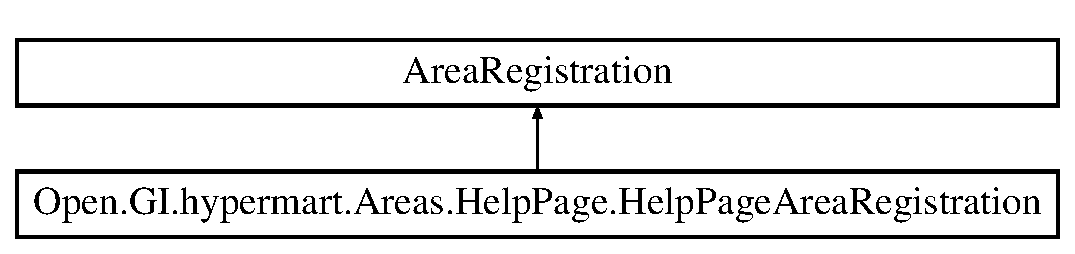
\includegraphics[height=2.000000cm]{class_open_1_1_g_i_1_1hypermart_1_1_areas_1_1_help_page_1_1_help_page_area_registration}
\end{center}
\end{figure}
\subsection*{Public Member Functions}
\begin{DoxyCompactItemize}
\item 
override void \textbf{ Register\+Area} (Area\+Registration\+Context context)
\begin{DoxyCompactList}\small\item\em Registers an area in an A\+S\+P.\+N\+ET M\+VC application using the specified area\textquotesingle{}s context information. \end{DoxyCompactList}\end{DoxyCompactItemize}
\subsection*{Properties}
\begin{DoxyCompactItemize}
\item 
override string \textbf{ Area\+Name}\hspace{0.3cm}{\ttfamily  [get]}
\begin{DoxyCompactList}\small\item\em Gets the name of the area to register. \end{DoxyCompactList}\end{DoxyCompactItemize}


\subsection{Detailed Description}


\begin{DoxySeeAlso}{See also}
System.\+Web.\+Mvc.\+Area\+Registration


\end{DoxySeeAlso}


Definition at line 10 of file Help\+Page\+Area\+Registration.\+cs.



\subsection{Member Function Documentation}
\mbox{\label{class_open_1_1_g_i_1_1hypermart_1_1_areas_1_1_help_page_1_1_help_page_area_registration_aee73751274402f096ce32ee010ef1a11}} 
\index{Open\+::\+G\+I\+::hypermart\+::\+Areas\+::\+Help\+Page\+::\+Help\+Page\+Area\+Registration@{Open\+::\+G\+I\+::hypermart\+::\+Areas\+::\+Help\+Page\+::\+Help\+Page\+Area\+Registration}!Register\+Area@{Register\+Area}}
\index{Register\+Area@{Register\+Area}!Open\+::\+G\+I\+::hypermart\+::\+Areas\+::\+Help\+Page\+::\+Help\+Page\+Area\+Registration@{Open\+::\+G\+I\+::hypermart\+::\+Areas\+::\+Help\+Page\+::\+Help\+Page\+Area\+Registration}}
\subsubsection{Register\+Area()}
{\footnotesize\ttfamily override void Open.\+G\+I.\+hypermart.\+Areas.\+Help\+Page.\+Help\+Page\+Area\+Registration.\+Register\+Area (\begin{DoxyParamCaption}\item[{Area\+Registration\+Context}]{context }\end{DoxyParamCaption})}



Registers an area in an A\+S\+P.\+N\+ET M\+VC application using the specified area\textquotesingle{}s context information. 


\begin{DoxyParams}{Parameters}
{\em context} & Encapsulates the information that is required in order to register the area.\\
\hline
\end{DoxyParams}


Definition at line 27 of file Help\+Page\+Area\+Registration.\+cs.



\subsection{Property Documentation}
\mbox{\label{class_open_1_1_g_i_1_1hypermart_1_1_areas_1_1_help_page_1_1_help_page_area_registration_a98b4d777a4852021b9a120b1eb5cd08a}} 
\index{Open\+::\+G\+I\+::hypermart\+::\+Areas\+::\+Help\+Page\+::\+Help\+Page\+Area\+Registration@{Open\+::\+G\+I\+::hypermart\+::\+Areas\+::\+Help\+Page\+::\+Help\+Page\+Area\+Registration}!Area\+Name@{Area\+Name}}
\index{Area\+Name@{Area\+Name}!Open\+::\+G\+I\+::hypermart\+::\+Areas\+::\+Help\+Page\+::\+Help\+Page\+Area\+Registration@{Open\+::\+G\+I\+::hypermart\+::\+Areas\+::\+Help\+Page\+::\+Help\+Page\+Area\+Registration}}
\subsubsection{Area\+Name}
{\footnotesize\ttfamily override string Open.\+G\+I.\+hypermart.\+Areas.\+Help\+Page.\+Help\+Page\+Area\+Registration.\+Area\+Name\hspace{0.3cm}{\ttfamily [get]}}



Gets the name of the area to register. 



Definition at line 16 of file Help\+Page\+Area\+Registration.\+cs.



The documentation for this class was generated from the following file\+:\begin{DoxyCompactItemize}
\item 
C\+:/\+Projects/\+App-\/\+Utility-\/\+Store/\+Open.\+G\+I.\+hypermart/\+Areas/\+Help\+Page/\textbf{ Help\+Page\+Area\+Registration.\+cs}\end{DoxyCompactItemize}

\hypertarget{class_open_1_1_g_i_1_1hypermart_1_1_areas_1_1_help_page_1_1_help_page_sample_generator}{}\section{Open.\+G\+I.\+hypermart.\+Areas.\+Help\+Page.\+Help\+Page\+Sample\+Generator Class Reference}
\label{class_open_1_1_g_i_1_1hypermart_1_1_areas_1_1_help_page_1_1_help_page_sample_generator}\index{Open.\+G\+I.\+hypermart.\+Areas.\+Help\+Page.\+Help\+Page\+Sample\+Generator@{Open.\+G\+I.\+hypermart.\+Areas.\+Help\+Page.\+Help\+Page\+Sample\+Generator}}


This class will generate the samples for the help page.  


\subsection*{Public Member Functions}
\begin{DoxyCompactItemize}
\item 
\hyperlink{class_open_1_1_g_i_1_1hypermart_1_1_areas_1_1_help_page_1_1_help_page_sample_generator_aa3984bba40389ce2ca9530e02a6a2eff}{Help\+Page\+Sample\+Generator} ()
\begin{DoxyCompactList}\small\item\em Initializes a new instance of the \hyperlink{class_open_1_1_g_i_1_1hypermart_1_1_areas_1_1_help_page_1_1_help_page_sample_generator}{Help\+Page\+Sample\+Generator} class. \end{DoxyCompactList}\item 
I\+Dictionary$<$ Media\+Type\+Header\+Value, object $>$ \hyperlink{class_open_1_1_g_i_1_1hypermart_1_1_areas_1_1_help_page_1_1_help_page_sample_generator_a1ae2a75ff1221fb53031799fbf2e4e65}{Get\+Sample\+Requests} (Api\+Description api)
\begin{DoxyCompactList}\small\item\em Gets the request body samples for a given Api\+Description. \end{DoxyCompactList}\item 
I\+Dictionary$<$ Media\+Type\+Header\+Value, object $>$ \hyperlink{class_open_1_1_g_i_1_1hypermart_1_1_areas_1_1_help_page_1_1_help_page_sample_generator_ac1b28b1a321875fe574c8db544326551}{Get\+Sample\+Responses} (Api\+Description api)
\begin{DoxyCompactList}\small\item\em Gets the response body samples for a given Api\+Description. \end{DoxyCompactList}\item 
virtual I\+Dictionary$<$ Media\+Type\+Header\+Value, object $>$ \hyperlink{class_open_1_1_g_i_1_1hypermart_1_1_areas_1_1_help_page_1_1_help_page_sample_generator_aa427225f9c3a32e667b908b071537f10}{Get\+Sample} (Api\+Description api, \hyperlink{namespace_open_1_1_g_i_1_1hypermart_1_1_areas_1_1_help_page_a96790152101b7f9c7e4ff518bb45c822}{Sample\+Direction} sample\+Direction)
\begin{DoxyCompactList}\small\item\em Gets the request or response body samples. \end{DoxyCompactList}\item 
virtual object \hyperlink{class_open_1_1_g_i_1_1hypermart_1_1_areas_1_1_help_page_1_1_help_page_sample_generator_aafd6b28c8518482fe8d7826d4a36a2bf}{Get\+Action\+Sample} (string controller\+Name, string action\+Name, I\+Enumerable$<$ string $>$ parameter\+Names, Type type, Media\+Type\+Formatter formatter, Media\+Type\+Header\+Value media\+Type, \hyperlink{namespace_open_1_1_g_i_1_1hypermart_1_1_areas_1_1_help_page_a96790152101b7f9c7e4ff518bb45c822}{Sample\+Direction} sample\+Direction)
\begin{DoxyCompactList}\small\item\em Search for samples that are provided directly through \hyperlink{class_open_1_1_g_i_1_1hypermart_1_1_areas_1_1_help_page_1_1_help_page_sample_generator_a6e94135c5b0f1c91af7a2662aa40d713}{Action\+Samples}. \end{DoxyCompactList}\item 
virtual object \hyperlink{class_open_1_1_g_i_1_1hypermart_1_1_areas_1_1_help_page_1_1_help_page_sample_generator_ae69a2233e30b8e1799fe175bc0e65821}{Get\+Sample\+Object} (Type type)
\begin{DoxyCompactList}\small\item\em Gets the sample object that will be serialized by the formatters. First, it will look at the \hyperlink{class_open_1_1_g_i_1_1hypermart_1_1_areas_1_1_help_page_1_1_help_page_sample_generator_a1a16afd9020493bb00d793ed79d0a056}{Sample\+Objects}. If no sample object is found, it will try to create one using Default\+Sample\+Object\+Factory (which wraps an \hyperlink{class_open_1_1_g_i_1_1hypermart_1_1_areas_1_1_help_page_1_1_object_generator}{Object\+Generator}) and other factories in \hyperlink{class_open_1_1_g_i_1_1hypermart_1_1_areas_1_1_help_page_1_1_help_page_sample_generator_a659aa13a69376385d931264d06fbd398}{Sample\+Object\+Factories}. \end{DoxyCompactList}\item 
virtual Type \hyperlink{class_open_1_1_g_i_1_1hypermart_1_1_areas_1_1_help_page_1_1_help_page_sample_generator_a64f0926946de3989be80507e6189fdc8}{Resolve\+Http\+Request\+Message\+Type} (Api\+Description api)
\begin{DoxyCompactList}\small\item\em Resolves the actual type of System.\+Net.\+Http.\+Object\+Content$<$\+T$>$ passed to the System.\+Net.\+Http.\+Http\+Request\+Message in an action. \end{DoxyCompactList}\item 
virtual Type \hyperlink{class_open_1_1_g_i_1_1hypermart_1_1_areas_1_1_help_page_1_1_help_page_sample_generator_aa2027a7a15a18958eb23c9a9d2407cda}{Resolve\+Type} (Api\+Description api, string controller\+Name, string action\+Name, I\+Enumerable$<$ string $>$ parameter\+Names, \hyperlink{namespace_open_1_1_g_i_1_1hypermart_1_1_areas_1_1_help_page_a96790152101b7f9c7e4ff518bb45c822}{Sample\+Direction} sample\+Direction, out Collection$<$ Media\+Type\+Formatter $>$ formatters)
\begin{DoxyCompactList}\small\item\em Resolves the type of the action parameter or return value when Http\+Request\+Message or Http\+Response\+Message is used. \end{DoxyCompactList}\item 
virtual object \hyperlink{class_open_1_1_g_i_1_1hypermart_1_1_areas_1_1_help_page_1_1_help_page_sample_generator_a2612cc414813ea500d4822a4cd17731a}{Write\+Sample\+Object\+Using\+Formatter} (Media\+Type\+Formatter formatter, object value, Type type, Media\+Type\+Header\+Value media\+Type)
\begin{DoxyCompactList}\small\item\em Writes the sample object using formatter. \end{DoxyCompactList}\end{DoxyCompactItemize}
\subsection*{Properties}
\begin{DoxyCompactItemize}
\item 
I\+Dictionary$<$ \hyperlink{class_open_1_1_g_i_1_1hypermart_1_1_areas_1_1_help_page_1_1_help_page_sample_key}{Help\+Page\+Sample\+Key}, Type $>$ \hyperlink{class_open_1_1_g_i_1_1hypermart_1_1_areas_1_1_help_page_1_1_help_page_sample_generator_a62bbf2941b3a4e2db28a546ae2fc5857}{Actual\+Http\+Message\+Types}\hspace{0.3cm}{\ttfamily  \mbox{[}get, set\mbox{]}}
\begin{DoxyCompactList}\small\item\em Gets C\+L\+R types that are used as the content of Http\+Request\+Message or Http\+Response\+Message. \end{DoxyCompactList}\item 
I\+Dictionary$<$ \hyperlink{class_open_1_1_g_i_1_1hypermart_1_1_areas_1_1_help_page_1_1_help_page_sample_key}{Help\+Page\+Sample\+Key}, object $>$ \hyperlink{class_open_1_1_g_i_1_1hypermart_1_1_areas_1_1_help_page_1_1_help_page_sample_generator_a6e94135c5b0f1c91af7a2662aa40d713}{Action\+Samples}\hspace{0.3cm}{\ttfamily  \mbox{[}get, set\mbox{]}}
\begin{DoxyCompactList}\small\item\em Gets the objects that are used directly as samples for certain actions. \end{DoxyCompactList}\item 
I\+Dictionary$<$ Type, object $>$ \hyperlink{class_open_1_1_g_i_1_1hypermart_1_1_areas_1_1_help_page_1_1_help_page_sample_generator_a1a16afd9020493bb00d793ed79d0a056}{Sample\+Objects}\hspace{0.3cm}{\ttfamily  \mbox{[}get, set\mbox{]}}
\begin{DoxyCompactList}\small\item\em Gets the objects that are serialized as samples by the supported formatters. \end{DoxyCompactList}\item 
I\+List$<$ Func$<$ \hyperlink{class_open_1_1_g_i_1_1hypermart_1_1_areas_1_1_help_page_1_1_help_page_sample_generator}{Help\+Page\+Sample\+Generator}, Type, object $>$ $>$ \hyperlink{class_open_1_1_g_i_1_1hypermart_1_1_areas_1_1_help_page_1_1_help_page_sample_generator_a659aa13a69376385d931264d06fbd398}{Sample\+Object\+Factories}\hspace{0.3cm}{\ttfamily  \mbox{[}get\mbox{]}}
\begin{DoxyCompactList}\small\item\em Gets factories for the objects that the supported formatters will serialize as samples. Processed in order, stopping when the factory successfully returns a non-\/ object. \end{DoxyCompactList}\end{DoxyCompactItemize}


\subsection{Detailed Description}
This class will generate the samples for the help page. 



Definition at line 21 of file Help\+Page\+Sample\+Generator.\+cs.



\subsection{Constructor \& Destructor Documentation}
\hypertarget{class_open_1_1_g_i_1_1hypermart_1_1_areas_1_1_help_page_1_1_help_page_sample_generator_aa3984bba40389ce2ca9530e02a6a2eff}{}\index{Open\+::\+G\+I\+::hypermart\+::\+Areas\+::\+Help\+Page\+::\+Help\+Page\+Sample\+Generator@{Open\+::\+G\+I\+::hypermart\+::\+Areas\+::\+Help\+Page\+::\+Help\+Page\+Sample\+Generator}!Help\+Page\+Sample\+Generator@{Help\+Page\+Sample\+Generator}}
\index{Help\+Page\+Sample\+Generator@{Help\+Page\+Sample\+Generator}!Open\+::\+G\+I\+::hypermart\+::\+Areas\+::\+Help\+Page\+::\+Help\+Page\+Sample\+Generator@{Open\+::\+G\+I\+::hypermart\+::\+Areas\+::\+Help\+Page\+::\+Help\+Page\+Sample\+Generator}}
\subsubsection[{Help\+Page\+Sample\+Generator()}]{\setlength{\rightskip}{0pt plus 5cm}Open.\+G\+I.\+hypermart.\+Areas.\+Help\+Page.\+Help\+Page\+Sample\+Generator.\+Help\+Page\+Sample\+Generator (
\begin{DoxyParamCaption}
{}
\end{DoxyParamCaption}
)}\label{class_open_1_1_g_i_1_1hypermart_1_1_areas_1_1_help_page_1_1_help_page_sample_generator_aa3984bba40389ce2ca9530e02a6a2eff}


Initializes a new instance of the \hyperlink{class_open_1_1_g_i_1_1hypermart_1_1_areas_1_1_help_page_1_1_help_page_sample_generator}{Help\+Page\+Sample\+Generator} class. 



Definition at line 26 of file Help\+Page\+Sample\+Generator.\+cs.



\subsection{Member Function Documentation}
\hypertarget{class_open_1_1_g_i_1_1hypermart_1_1_areas_1_1_help_page_1_1_help_page_sample_generator_aafd6b28c8518482fe8d7826d4a36a2bf}{}\index{Open\+::\+G\+I\+::hypermart\+::\+Areas\+::\+Help\+Page\+::\+Help\+Page\+Sample\+Generator@{Open\+::\+G\+I\+::hypermart\+::\+Areas\+::\+Help\+Page\+::\+Help\+Page\+Sample\+Generator}!Get\+Action\+Sample@{Get\+Action\+Sample}}
\index{Get\+Action\+Sample@{Get\+Action\+Sample}!Open\+::\+G\+I\+::hypermart\+::\+Areas\+::\+Help\+Page\+::\+Help\+Page\+Sample\+Generator@{Open\+::\+G\+I\+::hypermart\+::\+Areas\+::\+Help\+Page\+::\+Help\+Page\+Sample\+Generator}}
\subsubsection[{Get\+Action\+Sample(string controller\+Name, string action\+Name, I\+Enumerable$<$ string $>$ parameter\+Names, Type type, Media\+Type\+Formatter formatter, Media\+Type\+Header\+Value media\+Type, Sample\+Direction sample\+Direction)}]{\setlength{\rightskip}{0pt plus 5cm}virtual object Open.\+G\+I.\+hypermart.\+Areas.\+Help\+Page.\+Help\+Page\+Sample\+Generator.\+Get\+Action\+Sample (
\begin{DoxyParamCaption}
\item[{string}]{controller\+Name, }
\item[{string}]{action\+Name, }
\item[{I\+Enumerable$<$ string $>$}]{parameter\+Names, }
\item[{Type}]{type, }
\item[{Media\+Type\+Formatter}]{formatter, }
\item[{Media\+Type\+Header\+Value}]{media\+Type, }
\item[{{\bf Sample\+Direction}}]{sample\+Direction}
\end{DoxyParamCaption}
)\hspace{0.3cm}{\ttfamily [virtual]}}\label{class_open_1_1_g_i_1_1hypermart_1_1_areas_1_1_help_page_1_1_help_page_sample_generator_aafd6b28c8518482fe8d7826d4a36a2bf}


Search for samples that are provided directly through \hyperlink{class_open_1_1_g_i_1_1hypermart_1_1_areas_1_1_help_page_1_1_help_page_sample_generator_a6e94135c5b0f1c91af7a2662aa40d713}{Action\+Samples}. 


\begin{DoxyParams}{Parameters}
{\em controller\+Name} & Name of the controller.\\
\hline
{\em action\+Name} & Name of the action.\\
\hline
{\em parameter\+Names} & The parameter names.\\
\hline
{\em type} & The C\+L\+R type.\\
\hline
{\em formatter} & The formatter.\\
\hline
{\em media\+Type} & The media type.\\
\hline
{\em sample\+Direction} & The value indicating whether the sample is for a request or for a response.\\
\hline
\end{DoxyParams}
\begin{DoxyReturn}{Returns}
The sample that matches the parameters.
\end{DoxyReturn}


Definition at line 149 of file Help\+Page\+Sample\+Generator.\+cs.

\hypertarget{class_open_1_1_g_i_1_1hypermart_1_1_areas_1_1_help_page_1_1_help_page_sample_generator_aa427225f9c3a32e667b908b071537f10}{}\index{Open\+::\+G\+I\+::hypermart\+::\+Areas\+::\+Help\+Page\+::\+Help\+Page\+Sample\+Generator@{Open\+::\+G\+I\+::hypermart\+::\+Areas\+::\+Help\+Page\+::\+Help\+Page\+Sample\+Generator}!Get\+Sample@{Get\+Sample}}
\index{Get\+Sample@{Get\+Sample}!Open\+::\+G\+I\+::hypermart\+::\+Areas\+::\+Help\+Page\+::\+Help\+Page\+Sample\+Generator@{Open\+::\+G\+I\+::hypermart\+::\+Areas\+::\+Help\+Page\+::\+Help\+Page\+Sample\+Generator}}
\subsubsection[{Get\+Sample(\+Api\+Description api, Sample\+Direction sample\+Direction)}]{\setlength{\rightskip}{0pt plus 5cm}virtual I\+Dictionary$<$Media\+Type\+Header\+Value, object$>$ Open.\+G\+I.\+hypermart.\+Areas.\+Help\+Page.\+Help\+Page\+Sample\+Generator.\+Get\+Sample (
\begin{DoxyParamCaption}
\item[{Api\+Description}]{api, }
\item[{{\bf Sample\+Direction}}]{sample\+Direction}
\end{DoxyParamCaption}
)\hspace{0.3cm}{\ttfamily [virtual]}}\label{class_open_1_1_g_i_1_1hypermart_1_1_areas_1_1_help_page_1_1_help_page_sample_generator_aa427225f9c3a32e667b908b071537f10}


Gets the request or response body samples. 


\begin{DoxyParams}{Parameters}
{\em api} & The Api\+Description.\\
\hline
{\em sample\+Direction} & The value indicating whether the sample is for a request or for a response.\\
\hline
\end{DoxyParams}
\begin{DoxyReturn}{Returns}
The samples keyed by media type.
\end{DoxyReturn}


Definition at line 90 of file Help\+Page\+Sample\+Generator.\+cs.

\hypertarget{class_open_1_1_g_i_1_1hypermart_1_1_areas_1_1_help_page_1_1_help_page_sample_generator_ae69a2233e30b8e1799fe175bc0e65821}{}\index{Open\+::\+G\+I\+::hypermart\+::\+Areas\+::\+Help\+Page\+::\+Help\+Page\+Sample\+Generator@{Open\+::\+G\+I\+::hypermart\+::\+Areas\+::\+Help\+Page\+::\+Help\+Page\+Sample\+Generator}!Get\+Sample\+Object@{Get\+Sample\+Object}}
\index{Get\+Sample\+Object@{Get\+Sample\+Object}!Open\+::\+G\+I\+::hypermart\+::\+Areas\+::\+Help\+Page\+::\+Help\+Page\+Sample\+Generator@{Open\+::\+G\+I\+::hypermart\+::\+Areas\+::\+Help\+Page\+::\+Help\+Page\+Sample\+Generator}}
\subsubsection[{Get\+Sample\+Object(\+Type type)}]{\setlength{\rightskip}{0pt plus 5cm}virtual object Open.\+G\+I.\+hypermart.\+Areas.\+Help\+Page.\+Help\+Page\+Sample\+Generator.\+Get\+Sample\+Object (
\begin{DoxyParamCaption}
\item[{Type}]{type}
\end{DoxyParamCaption}
)\hspace{0.3cm}{\ttfamily [virtual]}}\label{class_open_1_1_g_i_1_1hypermart_1_1_areas_1_1_help_page_1_1_help_page_sample_generator_ae69a2233e30b8e1799fe175bc0e65821}


Gets the sample object that will be serialized by the formatters. First, it will look at the \hyperlink{class_open_1_1_g_i_1_1hypermart_1_1_areas_1_1_help_page_1_1_help_page_sample_generator_a1a16afd9020493bb00d793ed79d0a056}{Sample\+Objects}. If no sample object is found, it will try to create one using Default\+Sample\+Object\+Factory (which wraps an \hyperlink{class_open_1_1_g_i_1_1hypermart_1_1_areas_1_1_help_page_1_1_object_generator}{Object\+Generator}) and other factories in \hyperlink{class_open_1_1_g_i_1_1hypermart_1_1_areas_1_1_help_page_1_1_help_page_sample_generator_a659aa13a69376385d931264d06fbd398}{Sample\+Object\+Factories}. 


\begin{DoxyParams}{Parameters}
{\em type} & The type.\\
\hline
\end{DoxyParams}
\begin{DoxyReturn}{Returns}
The sample object.
\end{DoxyReturn}


Definition at line 178 of file Help\+Page\+Sample\+Generator.\+cs.

\hypertarget{class_open_1_1_g_i_1_1hypermart_1_1_areas_1_1_help_page_1_1_help_page_sample_generator_a1ae2a75ff1221fb53031799fbf2e4e65}{}\index{Open\+::\+G\+I\+::hypermart\+::\+Areas\+::\+Help\+Page\+::\+Help\+Page\+Sample\+Generator@{Open\+::\+G\+I\+::hypermart\+::\+Areas\+::\+Help\+Page\+::\+Help\+Page\+Sample\+Generator}!Get\+Sample\+Requests@{Get\+Sample\+Requests}}
\index{Get\+Sample\+Requests@{Get\+Sample\+Requests}!Open\+::\+G\+I\+::hypermart\+::\+Areas\+::\+Help\+Page\+::\+Help\+Page\+Sample\+Generator@{Open\+::\+G\+I\+::hypermart\+::\+Areas\+::\+Help\+Page\+::\+Help\+Page\+Sample\+Generator}}
\subsubsection[{Get\+Sample\+Requests(\+Api\+Description api)}]{\setlength{\rightskip}{0pt plus 5cm}I\+Dictionary$<$Media\+Type\+Header\+Value, object$>$ Open.\+G\+I.\+hypermart.\+Areas.\+Help\+Page.\+Help\+Page\+Sample\+Generator.\+Get\+Sample\+Requests (
\begin{DoxyParamCaption}
\item[{Api\+Description}]{api}
\end{DoxyParamCaption}
)}\label{class_open_1_1_g_i_1_1hypermart_1_1_areas_1_1_help_page_1_1_help_page_sample_generator_a1ae2a75ff1221fb53031799fbf2e4e65}


Gets the request body samples for a given Api\+Description. 


\begin{DoxyParams}{Parameters}
{\em api} & The Api\+Description.\\
\hline
\end{DoxyParams}
\begin{DoxyReturn}{Returns}
The samples keyed by media type.
\end{DoxyReturn}


Definition at line 69 of file Help\+Page\+Sample\+Generator.\+cs.

\hypertarget{class_open_1_1_g_i_1_1hypermart_1_1_areas_1_1_help_page_1_1_help_page_sample_generator_ac1b28b1a321875fe574c8db544326551}{}\index{Open\+::\+G\+I\+::hypermart\+::\+Areas\+::\+Help\+Page\+::\+Help\+Page\+Sample\+Generator@{Open\+::\+G\+I\+::hypermart\+::\+Areas\+::\+Help\+Page\+::\+Help\+Page\+Sample\+Generator}!Get\+Sample\+Responses@{Get\+Sample\+Responses}}
\index{Get\+Sample\+Responses@{Get\+Sample\+Responses}!Open\+::\+G\+I\+::hypermart\+::\+Areas\+::\+Help\+Page\+::\+Help\+Page\+Sample\+Generator@{Open\+::\+G\+I\+::hypermart\+::\+Areas\+::\+Help\+Page\+::\+Help\+Page\+Sample\+Generator}}
\subsubsection[{Get\+Sample\+Responses(\+Api\+Description api)}]{\setlength{\rightskip}{0pt plus 5cm}I\+Dictionary$<$Media\+Type\+Header\+Value, object$>$ Open.\+G\+I.\+hypermart.\+Areas.\+Help\+Page.\+Help\+Page\+Sample\+Generator.\+Get\+Sample\+Responses (
\begin{DoxyParamCaption}
\item[{Api\+Description}]{api}
\end{DoxyParamCaption}
)}\label{class_open_1_1_g_i_1_1hypermart_1_1_areas_1_1_help_page_1_1_help_page_sample_generator_ac1b28b1a321875fe574c8db544326551}


Gets the response body samples for a given Api\+Description. 


\begin{DoxyParams}{Parameters}
{\em api} & The Api\+Description.\\
\hline
\end{DoxyParams}
\begin{DoxyReturn}{Returns}
The samples keyed by media type.
\end{DoxyReturn}


Definition at line 79 of file Help\+Page\+Sample\+Generator.\+cs.

\hypertarget{class_open_1_1_g_i_1_1hypermart_1_1_areas_1_1_help_page_1_1_help_page_sample_generator_a64f0926946de3989be80507e6189fdc8}{}\index{Open\+::\+G\+I\+::hypermart\+::\+Areas\+::\+Help\+Page\+::\+Help\+Page\+Sample\+Generator@{Open\+::\+G\+I\+::hypermart\+::\+Areas\+::\+Help\+Page\+::\+Help\+Page\+Sample\+Generator}!Resolve\+Http\+Request\+Message\+Type@{Resolve\+Http\+Request\+Message\+Type}}
\index{Resolve\+Http\+Request\+Message\+Type@{Resolve\+Http\+Request\+Message\+Type}!Open\+::\+G\+I\+::hypermart\+::\+Areas\+::\+Help\+Page\+::\+Help\+Page\+Sample\+Generator@{Open\+::\+G\+I\+::hypermart\+::\+Areas\+::\+Help\+Page\+::\+Help\+Page\+Sample\+Generator}}
\subsubsection[{Resolve\+Http\+Request\+Message\+Type(\+Api\+Description api)}]{\setlength{\rightskip}{0pt plus 5cm}virtual Type Open.\+G\+I.\+hypermart.\+Areas.\+Help\+Page.\+Help\+Page\+Sample\+Generator.\+Resolve\+Http\+Request\+Message\+Type (
\begin{DoxyParamCaption}
\item[{Api\+Description}]{api}
\end{DoxyParamCaption}
)\hspace{0.3cm}{\ttfamily [virtual]}}\label{class_open_1_1_g_i_1_1hypermart_1_1_areas_1_1_help_page_1_1_help_page_sample_generator_a64f0926946de3989be80507e6189fdc8}


Resolves the actual type of System.\+Net.\+Http.\+Object\+Content$<$\+T$>$ passed to the System.\+Net.\+Http.\+Http\+Request\+Message in an action. 


\begin{DoxyParams}{Parameters}
{\em api} & The Api\+Description.\\
\hline
\end{DoxyParams}
\begin{DoxyReturn}{Returns}
The type.
\end{DoxyReturn}


Definition at line 215 of file Help\+Page\+Sample\+Generator.\+cs.

\hypertarget{class_open_1_1_g_i_1_1hypermart_1_1_areas_1_1_help_page_1_1_help_page_sample_generator_aa2027a7a15a18958eb23c9a9d2407cda}{}\index{Open\+::\+G\+I\+::hypermart\+::\+Areas\+::\+Help\+Page\+::\+Help\+Page\+Sample\+Generator@{Open\+::\+G\+I\+::hypermart\+::\+Areas\+::\+Help\+Page\+::\+Help\+Page\+Sample\+Generator}!Resolve\+Type@{Resolve\+Type}}
\index{Resolve\+Type@{Resolve\+Type}!Open\+::\+G\+I\+::hypermart\+::\+Areas\+::\+Help\+Page\+::\+Help\+Page\+Sample\+Generator@{Open\+::\+G\+I\+::hypermart\+::\+Areas\+::\+Help\+Page\+::\+Help\+Page\+Sample\+Generator}}
\subsubsection[{Resolve\+Type(\+Api\+Description api, string controller\+Name, string action\+Name, I\+Enumerable$<$ string $>$ parameter\+Names, Sample\+Direction sample\+Direction, out Collection$<$ Media\+Type\+Formatter $>$ formatters)}]{\setlength{\rightskip}{0pt plus 5cm}virtual Type Open.\+G\+I.\+hypermart.\+Areas.\+Help\+Page.\+Help\+Page\+Sample\+Generator.\+Resolve\+Type (
\begin{DoxyParamCaption}
\item[{Api\+Description}]{api, }
\item[{string}]{controller\+Name, }
\item[{string}]{action\+Name, }
\item[{I\+Enumerable$<$ string $>$}]{parameter\+Names, }
\item[{{\bf Sample\+Direction}}]{sample\+Direction, }
\item[{out Collection$<$ Media\+Type\+Formatter $>$}]{formatters}
\end{DoxyParamCaption}
)\hspace{0.3cm}{\ttfamily [virtual]}}\label{class_open_1_1_g_i_1_1hypermart_1_1_areas_1_1_help_page_1_1_help_page_sample_generator_aa2027a7a15a18958eb23c9a9d2407cda}


Resolves the type of the action parameter or return value when Http\+Request\+Message or Http\+Response\+Message is used. 


\begin{DoxyParams}{Parameters}
{\em api} & The Api\+Description.\\
\hline
{\em controller\+Name} & Name of the controller.\\
\hline
{\em action\+Name} & Name of the action.\\
\hline
{\em parameter\+Names} & The parameter names.\\
\hline
{\em sample\+Direction} & The value indicating whether the sample is for a request or a response.\\
\hline
{\em formatters} & The formatters.\\
\hline
\end{DoxyParams}


Definition at line 234 of file Help\+Page\+Sample\+Generator.\+cs.

\hypertarget{class_open_1_1_g_i_1_1hypermart_1_1_areas_1_1_help_page_1_1_help_page_sample_generator_a2612cc414813ea500d4822a4cd17731a}{}\index{Open\+::\+G\+I\+::hypermart\+::\+Areas\+::\+Help\+Page\+::\+Help\+Page\+Sample\+Generator@{Open\+::\+G\+I\+::hypermart\+::\+Areas\+::\+Help\+Page\+::\+Help\+Page\+Sample\+Generator}!Write\+Sample\+Object\+Using\+Formatter@{Write\+Sample\+Object\+Using\+Formatter}}
\index{Write\+Sample\+Object\+Using\+Formatter@{Write\+Sample\+Object\+Using\+Formatter}!Open\+::\+G\+I\+::hypermart\+::\+Areas\+::\+Help\+Page\+::\+Help\+Page\+Sample\+Generator@{Open\+::\+G\+I\+::hypermart\+::\+Areas\+::\+Help\+Page\+::\+Help\+Page\+Sample\+Generator}}
\subsubsection[{Write\+Sample\+Object\+Using\+Formatter(\+Media\+Type\+Formatter formatter, object value, Type type, Media\+Type\+Header\+Value media\+Type)}]{\setlength{\rightskip}{0pt plus 5cm}virtual object Open.\+G\+I.\+hypermart.\+Areas.\+Help\+Page.\+Help\+Page\+Sample\+Generator.\+Write\+Sample\+Object\+Using\+Formatter (
\begin{DoxyParamCaption}
\item[{Media\+Type\+Formatter}]{formatter, }
\item[{object}]{value, }
\item[{Type}]{type, }
\item[{Media\+Type\+Header\+Value}]{media\+Type}
\end{DoxyParamCaption}
)\hspace{0.3cm}{\ttfamily [virtual]}}\label{class_open_1_1_g_i_1_1hypermart_1_1_areas_1_1_help_page_1_1_help_page_sample_generator_a2612cc414813ea500d4822a4cd17731a}


Writes the sample object using formatter. 


\begin{DoxyParams}{Parameters}
{\em formatter} & The formatter.\\
\hline
{\em value} & The value.\\
\hline
{\em type} & The type.\\
\hline
{\em media\+Type} & Type of the media.\\
\hline
\end{DoxyParams}
\begin{DoxyReturn}{Returns}

\end{DoxyReturn}


Definition at line 288 of file Help\+Page\+Sample\+Generator.\+cs.



\subsection{Property Documentation}
\hypertarget{class_open_1_1_g_i_1_1hypermart_1_1_areas_1_1_help_page_1_1_help_page_sample_generator_a6e94135c5b0f1c91af7a2662aa40d713}{}\index{Open\+::\+G\+I\+::hypermart\+::\+Areas\+::\+Help\+Page\+::\+Help\+Page\+Sample\+Generator@{Open\+::\+G\+I\+::hypermart\+::\+Areas\+::\+Help\+Page\+::\+Help\+Page\+Sample\+Generator}!Action\+Samples@{Action\+Samples}}
\index{Action\+Samples@{Action\+Samples}!Open\+::\+G\+I\+::hypermart\+::\+Areas\+::\+Help\+Page\+::\+Help\+Page\+Sample\+Generator@{Open\+::\+G\+I\+::hypermart\+::\+Areas\+::\+Help\+Page\+::\+Help\+Page\+Sample\+Generator}}
\subsubsection[{Action\+Samples}]{\setlength{\rightskip}{0pt plus 5cm}I\+Dictionary$<${\bf Help\+Page\+Sample\+Key}, object$>$ Open.\+G\+I.\+hypermart.\+Areas.\+Help\+Page.\+Help\+Page\+Sample\+Generator.\+Action\+Samples\hspace{0.3cm}{\ttfamily [get]}, {\ttfamily [set]}}\label{class_open_1_1_g_i_1_1hypermart_1_1_areas_1_1_help_page_1_1_help_page_sample_generator_a6e94135c5b0f1c91af7a2662aa40d713}


Gets the objects that are used directly as samples for certain actions. 



Definition at line 45 of file Help\+Page\+Sample\+Generator.\+cs.

\hypertarget{class_open_1_1_g_i_1_1hypermart_1_1_areas_1_1_help_page_1_1_help_page_sample_generator_a62bbf2941b3a4e2db28a546ae2fc5857}{}\index{Open\+::\+G\+I\+::hypermart\+::\+Areas\+::\+Help\+Page\+::\+Help\+Page\+Sample\+Generator@{Open\+::\+G\+I\+::hypermart\+::\+Areas\+::\+Help\+Page\+::\+Help\+Page\+Sample\+Generator}!Actual\+Http\+Message\+Types@{Actual\+Http\+Message\+Types}}
\index{Actual\+Http\+Message\+Types@{Actual\+Http\+Message\+Types}!Open\+::\+G\+I\+::hypermart\+::\+Areas\+::\+Help\+Page\+::\+Help\+Page\+Sample\+Generator@{Open\+::\+G\+I\+::hypermart\+::\+Areas\+::\+Help\+Page\+::\+Help\+Page\+Sample\+Generator}}
\subsubsection[{Actual\+Http\+Message\+Types}]{\setlength{\rightskip}{0pt plus 5cm}I\+Dictionary$<${\bf Help\+Page\+Sample\+Key}, Type$>$ Open.\+G\+I.\+hypermart.\+Areas.\+Help\+Page.\+Help\+Page\+Sample\+Generator.\+Actual\+Http\+Message\+Types\hspace{0.3cm}{\ttfamily [get]}, {\ttfamily [set]}}\label{class_open_1_1_g_i_1_1hypermart_1_1_areas_1_1_help_page_1_1_help_page_sample_generator_a62bbf2941b3a4e2db28a546ae2fc5857}


Gets C\+L\+R types that are used as the content of Http\+Request\+Message or Http\+Response\+Message. 



Definition at line 40 of file Help\+Page\+Sample\+Generator.\+cs.

\hypertarget{class_open_1_1_g_i_1_1hypermart_1_1_areas_1_1_help_page_1_1_help_page_sample_generator_a659aa13a69376385d931264d06fbd398}{}\index{Open\+::\+G\+I\+::hypermart\+::\+Areas\+::\+Help\+Page\+::\+Help\+Page\+Sample\+Generator@{Open\+::\+G\+I\+::hypermart\+::\+Areas\+::\+Help\+Page\+::\+Help\+Page\+Sample\+Generator}!Sample\+Object\+Factories@{Sample\+Object\+Factories}}
\index{Sample\+Object\+Factories@{Sample\+Object\+Factories}!Open\+::\+G\+I\+::hypermart\+::\+Areas\+::\+Help\+Page\+::\+Help\+Page\+Sample\+Generator@{Open\+::\+G\+I\+::hypermart\+::\+Areas\+::\+Help\+Page\+::\+Help\+Page\+Sample\+Generator}}
\subsubsection[{Sample\+Object\+Factories}]{\setlength{\rightskip}{0pt plus 5cm}I\+List$<$Func$<${\bf Help\+Page\+Sample\+Generator}, Type, object$>$ $>$ Open.\+G\+I.\+hypermart.\+Areas.\+Help\+Page.\+Help\+Page\+Sample\+Generator.\+Sample\+Object\+Factories\hspace{0.3cm}{\ttfamily [get]}}\label{class_open_1_1_g_i_1_1hypermart_1_1_areas_1_1_help_page_1_1_help_page_sample_generator_a659aa13a69376385d931264d06fbd398}


Gets factories for the objects that the supported formatters will serialize as samples. Processed in order, stopping when the factory successfully returns a non-\/ object. 

Collection includes just \hyperlink{class_open_1_1_g_i_1_1hypermart_1_1_areas_1_1_help_page_1_1_object_generator_a118924d1ff5f565e6e9c2893d36f35d2}{Object\+Generator.\+Generate\+Object(\+Type)} initially. Use 
\begin{DoxyCode}
\hyperlink{class_open_1_1_g_i_1_1hypermart_1_1_areas_1_1_help_page_1_1_help_page_sample_generator_a659aa13a69376385d931264d06fbd398}{SampleObjectFactories}.Insert(0, func)
\end{DoxyCode}
 to provide an override and 
\begin{DoxyCode}
\hyperlink{class_open_1_1_g_i_1_1hypermart_1_1_areas_1_1_help_page_1_1_help_page_sample_generator_a659aa13a69376385d931264d06fbd398}{SampleObjectFactories}.Add(func)
\end{DoxyCode}
 to provide a fallback.

Definition at line 62 of file Help\+Page\+Sample\+Generator.\+cs.

\hypertarget{class_open_1_1_g_i_1_1hypermart_1_1_areas_1_1_help_page_1_1_help_page_sample_generator_a1a16afd9020493bb00d793ed79d0a056}{}\index{Open\+::\+G\+I\+::hypermart\+::\+Areas\+::\+Help\+Page\+::\+Help\+Page\+Sample\+Generator@{Open\+::\+G\+I\+::hypermart\+::\+Areas\+::\+Help\+Page\+::\+Help\+Page\+Sample\+Generator}!Sample\+Objects@{Sample\+Objects}}
\index{Sample\+Objects@{Sample\+Objects}!Open\+::\+G\+I\+::hypermart\+::\+Areas\+::\+Help\+Page\+::\+Help\+Page\+Sample\+Generator@{Open\+::\+G\+I\+::hypermart\+::\+Areas\+::\+Help\+Page\+::\+Help\+Page\+Sample\+Generator}}
\subsubsection[{Sample\+Objects}]{\setlength{\rightskip}{0pt plus 5cm}I\+Dictionary$<$Type, object$>$ Open.\+G\+I.\+hypermart.\+Areas.\+Help\+Page.\+Help\+Page\+Sample\+Generator.\+Sample\+Objects\hspace{0.3cm}{\ttfamily [get]}, {\ttfamily [set]}}\label{class_open_1_1_g_i_1_1hypermart_1_1_areas_1_1_help_page_1_1_help_page_sample_generator_a1a16afd9020493bb00d793ed79d0a056}


Gets the objects that are serialized as samples by the supported formatters. 



Definition at line 50 of file Help\+Page\+Sample\+Generator.\+cs.



The documentation for this class was generated from the following file\+:\begin{DoxyCompactItemize}
\item 
C\+:/\+Projects/\+App-\/\+Utility-\/\+Store/\+Open.\+G\+I.\+hypermart/\+Areas/\+Help\+Page/\+Sample\+Generation/\hyperlink{_help_page_sample_generator_8cs}{Help\+Page\+Sample\+Generator.\+cs}\end{DoxyCompactItemize}

\hypertarget{class_open_1_1_g_i_1_1hypermart_1_1_areas_1_1_help_page_1_1_help_page_sample_key}{}\section{Open.\+G\+I.\+hypermart.\+Areas.\+Help\+Page.\+Help\+Page\+Sample\+Key Class Reference}
\label{class_open_1_1_g_i_1_1hypermart_1_1_areas_1_1_help_page_1_1_help_page_sample_key}\index{Open.\+G\+I.\+hypermart.\+Areas.\+Help\+Page.\+Help\+Page\+Sample\+Key@{Open.\+G\+I.\+hypermart.\+Areas.\+Help\+Page.\+Help\+Page\+Sample\+Key}}


This is used to identify the place where the sample should be applied.  


\subsection*{Public Member Functions}
\begin{DoxyCompactItemize}
\item 
\hyperlink{class_open_1_1_g_i_1_1hypermart_1_1_areas_1_1_help_page_1_1_help_page_sample_key_ad8a76b6a8eb3e52035d2dd20d0a9706b}{Help\+Page\+Sample\+Key} (Media\+Type\+Header\+Value media\+Type)
\begin{DoxyCompactList}\small\item\em Creates a new \hyperlink{class_open_1_1_g_i_1_1hypermart_1_1_areas_1_1_help_page_1_1_help_page_sample_key}{Help\+Page\+Sample\+Key} based on media type. \end{DoxyCompactList}\item 
\hyperlink{class_open_1_1_g_i_1_1hypermart_1_1_areas_1_1_help_page_1_1_help_page_sample_key_a17332c9908a0efd7d9c68d15f2217170}{Help\+Page\+Sample\+Key} (Media\+Type\+Header\+Value media\+Type, Type type)
\begin{DoxyCompactList}\small\item\em Creates a new \hyperlink{class_open_1_1_g_i_1_1hypermart_1_1_areas_1_1_help_page_1_1_help_page_sample_key}{Help\+Page\+Sample\+Key} based on media type and C\+L\+R type. \end{DoxyCompactList}\item 
\hyperlink{class_open_1_1_g_i_1_1hypermart_1_1_areas_1_1_help_page_1_1_help_page_sample_key_a98e3f2c1797d9c12a29d6aaca315fef9}{Help\+Page\+Sample\+Key} (\hyperlink{namespace_open_1_1_g_i_1_1hypermart_1_1_areas_1_1_help_page_a96790152101b7f9c7e4ff518bb45c822}{Sample\+Direction} sample\+Direction, string controller\+Name, string action\+Name, I\+Enumerable$<$ string $>$ parameter\+Names)
\begin{DoxyCompactList}\small\item\em Creates a new \hyperlink{class_open_1_1_g_i_1_1hypermart_1_1_areas_1_1_help_page_1_1_help_page_sample_key}{Help\+Page\+Sample\+Key} based on \hyperlink{class_open_1_1_g_i_1_1hypermart_1_1_areas_1_1_help_page_1_1_help_page_sample_key_a62a3b3c50ce55cf2b20b4f859776f884}{Sample\+Direction}, controller name, action name and parameter names. \end{DoxyCompactList}\item 
\hyperlink{class_open_1_1_g_i_1_1hypermart_1_1_areas_1_1_help_page_1_1_help_page_sample_key_ad0be4fe1feb2ef2719dd3f2cb649a987}{Help\+Page\+Sample\+Key} (Media\+Type\+Header\+Value media\+Type, \hyperlink{namespace_open_1_1_g_i_1_1hypermart_1_1_areas_1_1_help_page_a96790152101b7f9c7e4ff518bb45c822}{Sample\+Direction} sample\+Direction, string controller\+Name, string action\+Name, I\+Enumerable$<$ string $>$ parameter\+Names)
\begin{DoxyCompactList}\small\item\em Creates a new \hyperlink{class_open_1_1_g_i_1_1hypermart_1_1_areas_1_1_help_page_1_1_help_page_sample_key}{Help\+Page\+Sample\+Key} based on media type, \hyperlink{class_open_1_1_g_i_1_1hypermart_1_1_areas_1_1_help_page_1_1_help_page_sample_key_a62a3b3c50ce55cf2b20b4f859776f884}{Sample\+Direction}, controller name, action name and parameter names. \end{DoxyCompactList}\item 
override bool \hyperlink{class_open_1_1_g_i_1_1hypermart_1_1_areas_1_1_help_page_1_1_help_page_sample_key_a6f27772d78ce8643c31153497bdff9b7}{Equals} (object obj)
\begin{DoxyCompactList}\small\item\em Determines whether the specified System.\+Object, is equal to this instance. \end{DoxyCompactList}\item 
override int \hyperlink{class_open_1_1_g_i_1_1hypermart_1_1_areas_1_1_help_page_1_1_help_page_sample_key_a232891dfae35aa54606577e755c3b3c3}{Get\+Hash\+Code} ()
\begin{DoxyCompactList}\small\item\em Returns a hash code for this instance. \end{DoxyCompactList}\end{DoxyCompactItemize}
\subsection*{Properties}
\begin{DoxyCompactItemize}
\item 
string \hyperlink{class_open_1_1_g_i_1_1hypermart_1_1_areas_1_1_help_page_1_1_help_page_sample_key_a8045e8479b1f6b2f1bb4f51c96fc7591}{Controller\+Name}\hspace{0.3cm}{\ttfamily  \mbox{[}get\mbox{]}}
\begin{DoxyCompactList}\small\item\em Gets the name of the controller. \end{DoxyCompactList}\item 
string \hyperlink{class_open_1_1_g_i_1_1hypermart_1_1_areas_1_1_help_page_1_1_help_page_sample_key_aaa937f6039e7b88ba4fade25831f0295}{Action\+Name}\hspace{0.3cm}{\ttfamily  \mbox{[}get\mbox{]}}
\begin{DoxyCompactList}\small\item\em Gets the name of the action. \end{DoxyCompactList}\item 
Media\+Type\+Header\+Value \hyperlink{class_open_1_1_g_i_1_1hypermart_1_1_areas_1_1_help_page_1_1_help_page_sample_key_a55d7490220ed44dd3611a3982b802850}{Media\+Type}\hspace{0.3cm}{\ttfamily  \mbox{[}get\mbox{]}}
\begin{DoxyCompactList}\small\item\em Gets the media type. \end{DoxyCompactList}\item 
Hash\+Set$<$ string $>$ \hyperlink{class_open_1_1_g_i_1_1hypermart_1_1_areas_1_1_help_page_1_1_help_page_sample_key_af57a533cea792e25a70fda6695a65c46}{Parameter\+Names}\hspace{0.3cm}{\ttfamily  \mbox{[}get\mbox{]}}
\begin{DoxyCompactList}\small\item\em Gets the parameter names. \end{DoxyCompactList}\item 
Type \hyperlink{class_open_1_1_g_i_1_1hypermart_1_1_areas_1_1_help_page_1_1_help_page_sample_key_afa5b00d332331b114e9391367bda2bf0}{Parameter\+Type}\hspace{0.3cm}{\ttfamily  \mbox{[}get\mbox{]}}
\begin{DoxyCompactList}\small\item\em Gets the type of the parameter. \end{DoxyCompactList}\item 
\hyperlink{namespace_open_1_1_g_i_1_1hypermart_1_1_areas_1_1_help_page_a96790152101b7f9c7e4ff518bb45c822}{Sample\+Direction} \hyperlink{class_open_1_1_g_i_1_1hypermart_1_1_areas_1_1_help_page_1_1_help_page_sample_key_a62a3b3c50ce55cf2b20b4f859776f884}{Sample\+Direction}\hspace{0.3cm}{\ttfamily  \mbox{[}get\mbox{]}}
\begin{DoxyCompactList}\small\item\em Gets the \hyperlink{class_open_1_1_g_i_1_1hypermart_1_1_areas_1_1_help_page_1_1_help_page_sample_key_a62a3b3c50ce55cf2b20b4f859776f884}{Sample\+Direction}. \end{DoxyCompactList}\end{DoxyCompactItemize}


\subsection{Detailed Description}
This is used to identify the place where the sample should be applied. 



Definition at line 11 of file Help\+Page\+Sample\+Key.\+cs.



\subsection{Constructor \& Destructor Documentation}
\hypertarget{class_open_1_1_g_i_1_1hypermart_1_1_areas_1_1_help_page_1_1_help_page_sample_key_ad8a76b6a8eb3e52035d2dd20d0a9706b}{}\index{Open\+::\+G\+I\+::hypermart\+::\+Areas\+::\+Help\+Page\+::\+Help\+Page\+Sample\+Key@{Open\+::\+G\+I\+::hypermart\+::\+Areas\+::\+Help\+Page\+::\+Help\+Page\+Sample\+Key}!Help\+Page\+Sample\+Key@{Help\+Page\+Sample\+Key}}
\index{Help\+Page\+Sample\+Key@{Help\+Page\+Sample\+Key}!Open\+::\+G\+I\+::hypermart\+::\+Areas\+::\+Help\+Page\+::\+Help\+Page\+Sample\+Key@{Open\+::\+G\+I\+::hypermart\+::\+Areas\+::\+Help\+Page\+::\+Help\+Page\+Sample\+Key}}
\subsubsection[{Help\+Page\+Sample\+Key(\+Media\+Type\+Header\+Value media\+Type)}]{\setlength{\rightskip}{0pt plus 5cm}Open.\+G\+I.\+hypermart.\+Areas.\+Help\+Page.\+Help\+Page\+Sample\+Key.\+Help\+Page\+Sample\+Key (
\begin{DoxyParamCaption}
\item[{Media\+Type\+Header\+Value}]{media\+Type}
\end{DoxyParamCaption}
)}\label{class_open_1_1_g_i_1_1hypermart_1_1_areas_1_1_help_page_1_1_help_page_sample_key_ad8a76b6a8eb3e52035d2dd20d0a9706b}


Creates a new \hyperlink{class_open_1_1_g_i_1_1hypermart_1_1_areas_1_1_help_page_1_1_help_page_sample_key}{Help\+Page\+Sample\+Key} based on media type. 


\begin{DoxyParams}{Parameters}
{\em media\+Type} & The media type.\\
\hline
\end{DoxyParams}


Definition at line 17 of file Help\+Page\+Sample\+Key.\+cs.

\hypertarget{class_open_1_1_g_i_1_1hypermart_1_1_areas_1_1_help_page_1_1_help_page_sample_key_a17332c9908a0efd7d9c68d15f2217170}{}\index{Open\+::\+G\+I\+::hypermart\+::\+Areas\+::\+Help\+Page\+::\+Help\+Page\+Sample\+Key@{Open\+::\+G\+I\+::hypermart\+::\+Areas\+::\+Help\+Page\+::\+Help\+Page\+Sample\+Key}!Help\+Page\+Sample\+Key@{Help\+Page\+Sample\+Key}}
\index{Help\+Page\+Sample\+Key@{Help\+Page\+Sample\+Key}!Open\+::\+G\+I\+::hypermart\+::\+Areas\+::\+Help\+Page\+::\+Help\+Page\+Sample\+Key@{Open\+::\+G\+I\+::hypermart\+::\+Areas\+::\+Help\+Page\+::\+Help\+Page\+Sample\+Key}}
\subsubsection[{Help\+Page\+Sample\+Key(\+Media\+Type\+Header\+Value media\+Type, Type type)}]{\setlength{\rightskip}{0pt plus 5cm}Open.\+G\+I.\+hypermart.\+Areas.\+Help\+Page.\+Help\+Page\+Sample\+Key.\+Help\+Page\+Sample\+Key (
\begin{DoxyParamCaption}
\item[{Media\+Type\+Header\+Value}]{media\+Type, }
\item[{Type}]{type}
\end{DoxyParamCaption}
)}\label{class_open_1_1_g_i_1_1hypermart_1_1_areas_1_1_help_page_1_1_help_page_sample_key_a17332c9908a0efd7d9c68d15f2217170}


Creates a new \hyperlink{class_open_1_1_g_i_1_1hypermart_1_1_areas_1_1_help_page_1_1_help_page_sample_key}{Help\+Page\+Sample\+Key} based on media type and C\+L\+R type. 


\begin{DoxyParams}{Parameters}
{\em media\+Type} & The media type.\\
\hline
{\em type} & The C\+L\+R type.\\
\hline
\end{DoxyParams}


Definition at line 35 of file Help\+Page\+Sample\+Key.\+cs.

\hypertarget{class_open_1_1_g_i_1_1hypermart_1_1_areas_1_1_help_page_1_1_help_page_sample_key_a98e3f2c1797d9c12a29d6aaca315fef9}{}\index{Open\+::\+G\+I\+::hypermart\+::\+Areas\+::\+Help\+Page\+::\+Help\+Page\+Sample\+Key@{Open\+::\+G\+I\+::hypermart\+::\+Areas\+::\+Help\+Page\+::\+Help\+Page\+Sample\+Key}!Help\+Page\+Sample\+Key@{Help\+Page\+Sample\+Key}}
\index{Help\+Page\+Sample\+Key@{Help\+Page\+Sample\+Key}!Open\+::\+G\+I\+::hypermart\+::\+Areas\+::\+Help\+Page\+::\+Help\+Page\+Sample\+Key@{Open\+::\+G\+I\+::hypermart\+::\+Areas\+::\+Help\+Page\+::\+Help\+Page\+Sample\+Key}}
\subsubsection[{Help\+Page\+Sample\+Key(\+Sample\+Direction sample\+Direction, string controller\+Name, string action\+Name, I\+Enumerable$<$ string $>$ parameter\+Names)}]{\setlength{\rightskip}{0pt plus 5cm}Open.\+G\+I.\+hypermart.\+Areas.\+Help\+Page.\+Help\+Page\+Sample\+Key.\+Help\+Page\+Sample\+Key (
\begin{DoxyParamCaption}
\item[{{\bf Sample\+Direction}}]{sample\+Direction, }
\item[{string}]{controller\+Name, }
\item[{string}]{action\+Name, }
\item[{I\+Enumerable$<$ string $>$}]{parameter\+Names}
\end{DoxyParamCaption}
)}\label{class_open_1_1_g_i_1_1hypermart_1_1_areas_1_1_help_page_1_1_help_page_sample_key_a98e3f2c1797d9c12a29d6aaca315fef9}


Creates a new \hyperlink{class_open_1_1_g_i_1_1hypermart_1_1_areas_1_1_help_page_1_1_help_page_sample_key}{Help\+Page\+Sample\+Key} based on \hyperlink{class_open_1_1_g_i_1_1hypermart_1_1_areas_1_1_help_page_1_1_help_page_sample_key_a62a3b3c50ce55cf2b20b4f859776f884}{Sample\+Direction}, controller name, action name and parameter names. 


\begin{DoxyParams}{Parameters}
{\em sample\+Direction} & The \hyperlink{class_open_1_1_g_i_1_1hypermart_1_1_areas_1_1_help_page_1_1_help_page_sample_key_a62a3b3c50ce55cf2b20b4f859776f884}{Sample\+Direction}.\\
\hline
{\em controller\+Name} & Name of the controller.\\
\hline
{\em action\+Name} & Name of the action.\\
\hline
{\em parameter\+Names} & The parameter names.\\
\hline
\end{DoxyParams}


Definition at line 53 of file Help\+Page\+Sample\+Key.\+cs.

\hypertarget{class_open_1_1_g_i_1_1hypermart_1_1_areas_1_1_help_page_1_1_help_page_sample_key_ad0be4fe1feb2ef2719dd3f2cb649a987}{}\index{Open\+::\+G\+I\+::hypermart\+::\+Areas\+::\+Help\+Page\+::\+Help\+Page\+Sample\+Key@{Open\+::\+G\+I\+::hypermart\+::\+Areas\+::\+Help\+Page\+::\+Help\+Page\+Sample\+Key}!Help\+Page\+Sample\+Key@{Help\+Page\+Sample\+Key}}
\index{Help\+Page\+Sample\+Key@{Help\+Page\+Sample\+Key}!Open\+::\+G\+I\+::hypermart\+::\+Areas\+::\+Help\+Page\+::\+Help\+Page\+Sample\+Key@{Open\+::\+G\+I\+::hypermart\+::\+Areas\+::\+Help\+Page\+::\+Help\+Page\+Sample\+Key}}
\subsubsection[{Help\+Page\+Sample\+Key(\+Media\+Type\+Header\+Value media\+Type, Sample\+Direction sample\+Direction, string controller\+Name, string action\+Name, I\+Enumerable$<$ string $>$ parameter\+Names)}]{\setlength{\rightskip}{0pt plus 5cm}Open.\+G\+I.\+hypermart.\+Areas.\+Help\+Page.\+Help\+Page\+Sample\+Key.\+Help\+Page\+Sample\+Key (
\begin{DoxyParamCaption}
\item[{Media\+Type\+Header\+Value}]{media\+Type, }
\item[{{\bf Sample\+Direction}}]{sample\+Direction, }
\item[{string}]{controller\+Name, }
\item[{string}]{action\+Name, }
\item[{I\+Enumerable$<$ string $>$}]{parameter\+Names}
\end{DoxyParamCaption}
)}\label{class_open_1_1_g_i_1_1hypermart_1_1_areas_1_1_help_page_1_1_help_page_sample_key_ad0be4fe1feb2ef2719dd3f2cb649a987}


Creates a new \hyperlink{class_open_1_1_g_i_1_1hypermart_1_1_areas_1_1_help_page_1_1_help_page_sample_key}{Help\+Page\+Sample\+Key} based on media type, \hyperlink{class_open_1_1_g_i_1_1hypermart_1_1_areas_1_1_help_page_1_1_help_page_sample_key_a62a3b3c50ce55cf2b20b4f859776f884}{Sample\+Direction}, controller name, action name and parameter names. 


\begin{DoxyParams}{Parameters}
{\em media\+Type} & The media type.\\
\hline
{\em sample\+Direction} & The \hyperlink{class_open_1_1_g_i_1_1hypermart_1_1_areas_1_1_help_page_1_1_help_page_sample_key_a62a3b3c50ce55cf2b20b4f859776f884}{Sample\+Direction}.\\
\hline
{\em controller\+Name} & Name of the controller.\\
\hline
{\em action\+Name} & Name of the action.\\
\hline
{\em parameter\+Names} & The parameter names.\\
\hline
\end{DoxyParams}


Definition at line 86 of file Help\+Page\+Sample\+Key.\+cs.



\subsection{Member Function Documentation}
\hypertarget{class_open_1_1_g_i_1_1hypermart_1_1_areas_1_1_help_page_1_1_help_page_sample_key_a6f27772d78ce8643c31153497bdff9b7}{}\index{Open\+::\+G\+I\+::hypermart\+::\+Areas\+::\+Help\+Page\+::\+Help\+Page\+Sample\+Key@{Open\+::\+G\+I\+::hypermart\+::\+Areas\+::\+Help\+Page\+::\+Help\+Page\+Sample\+Key}!Equals@{Equals}}
\index{Equals@{Equals}!Open\+::\+G\+I\+::hypermart\+::\+Areas\+::\+Help\+Page\+::\+Help\+Page\+Sample\+Key@{Open\+::\+G\+I\+::hypermart\+::\+Areas\+::\+Help\+Page\+::\+Help\+Page\+Sample\+Key}}
\subsubsection[{Equals(object obj)}]{\setlength{\rightskip}{0pt plus 5cm}override bool Open.\+G\+I.\+hypermart.\+Areas.\+Help\+Page.\+Help\+Page\+Sample\+Key.\+Equals (
\begin{DoxyParamCaption}
\item[{object}]{obj}
\end{DoxyParamCaption}
)}\label{class_open_1_1_g_i_1_1hypermart_1_1_areas_1_1_help_page_1_1_help_page_sample_key_a6f27772d78ce8643c31153497bdff9b7}


Determines whether the specified System.\+Object, is equal to this instance. 


\begin{DoxyParams}{Parameters}
{\em obj} & The System.\+Object to compare with this instance.\\
\hline
\end{DoxyParams}
\begin{DoxyReturn}{Returns}
{\ttfamily true} if the specified System.\+Object is equal to this instance; otherwise, {\ttfamily false}. 
\end{DoxyReturn}


Definition at line 146 of file Help\+Page\+Sample\+Key.\+cs.

\hypertarget{class_open_1_1_g_i_1_1hypermart_1_1_areas_1_1_help_page_1_1_help_page_sample_key_a232891dfae35aa54606577e755c3b3c3}{}\index{Open\+::\+G\+I\+::hypermart\+::\+Areas\+::\+Help\+Page\+::\+Help\+Page\+Sample\+Key@{Open\+::\+G\+I\+::hypermart\+::\+Areas\+::\+Help\+Page\+::\+Help\+Page\+Sample\+Key}!Get\+Hash\+Code@{Get\+Hash\+Code}}
\index{Get\+Hash\+Code@{Get\+Hash\+Code}!Open\+::\+G\+I\+::hypermart\+::\+Areas\+::\+Help\+Page\+::\+Help\+Page\+Sample\+Key@{Open\+::\+G\+I\+::hypermart\+::\+Areas\+::\+Help\+Page\+::\+Help\+Page\+Sample\+Key}}
\subsubsection[{Get\+Hash\+Code()}]{\setlength{\rightskip}{0pt plus 5cm}override int Open.\+G\+I.\+hypermart.\+Areas.\+Help\+Page.\+Help\+Page\+Sample\+Key.\+Get\+Hash\+Code (
\begin{DoxyParamCaption}
{}
\end{DoxyParamCaption}
)}\label{class_open_1_1_g_i_1_1hypermart_1_1_areas_1_1_help_page_1_1_help_page_sample_key_a232891dfae35aa54606577e755c3b3c3}


Returns a hash code for this instance. 

\begin{DoxyReturn}{Returns}
A hash code for this instance, suitable for use in hashing algorithms and data structures like a hash table. 
\end{DoxyReturn}


Definition at line 168 of file Help\+Page\+Sample\+Key.\+cs.



\subsection{Property Documentation}
\hypertarget{class_open_1_1_g_i_1_1hypermart_1_1_areas_1_1_help_page_1_1_help_page_sample_key_aaa937f6039e7b88ba4fade25831f0295}{}\index{Open\+::\+G\+I\+::hypermart\+::\+Areas\+::\+Help\+Page\+::\+Help\+Page\+Sample\+Key@{Open\+::\+G\+I\+::hypermart\+::\+Areas\+::\+Help\+Page\+::\+Help\+Page\+Sample\+Key}!Action\+Name@{Action\+Name}}
\index{Action\+Name@{Action\+Name}!Open\+::\+G\+I\+::hypermart\+::\+Areas\+::\+Help\+Page\+::\+Help\+Page\+Sample\+Key@{Open\+::\+G\+I\+::hypermart\+::\+Areas\+::\+Help\+Page\+::\+Help\+Page\+Sample\+Key}}
\subsubsection[{Action\+Name}]{\setlength{\rightskip}{0pt plus 5cm}string Open.\+G\+I.\+hypermart.\+Areas.\+Help\+Page.\+Help\+Page\+Sample\+Key.\+Action\+Name\hspace{0.3cm}{\ttfamily [get]}}\label{class_open_1_1_g_i_1_1hypermart_1_1_areas_1_1_help_page_1_1_help_page_sample_key_aaa937f6039e7b88ba4fade25831f0295}


Gets the name of the action. 

The name of the action. 

Definition at line 111 of file Help\+Page\+Sample\+Key.\+cs.

\hypertarget{class_open_1_1_g_i_1_1hypermart_1_1_areas_1_1_help_page_1_1_help_page_sample_key_a8045e8479b1f6b2f1bb4f51c96fc7591}{}\index{Open\+::\+G\+I\+::hypermart\+::\+Areas\+::\+Help\+Page\+::\+Help\+Page\+Sample\+Key@{Open\+::\+G\+I\+::hypermart\+::\+Areas\+::\+Help\+Page\+::\+Help\+Page\+Sample\+Key}!Controller\+Name@{Controller\+Name}}
\index{Controller\+Name@{Controller\+Name}!Open\+::\+G\+I\+::hypermart\+::\+Areas\+::\+Help\+Page\+::\+Help\+Page\+Sample\+Key@{Open\+::\+G\+I\+::hypermart\+::\+Areas\+::\+Help\+Page\+::\+Help\+Page\+Sample\+Key}}
\subsubsection[{Controller\+Name}]{\setlength{\rightskip}{0pt plus 5cm}string Open.\+G\+I.\+hypermart.\+Areas.\+Help\+Page.\+Help\+Page\+Sample\+Key.\+Controller\+Name\hspace{0.3cm}{\ttfamily [get]}}\label{class_open_1_1_g_i_1_1hypermart_1_1_areas_1_1_help_page_1_1_help_page_sample_key_a8045e8479b1f6b2f1bb4f51c96fc7591}


Gets the name of the controller. 

The name of the controller. 

Definition at line 103 of file Help\+Page\+Sample\+Key.\+cs.

\hypertarget{class_open_1_1_g_i_1_1hypermart_1_1_areas_1_1_help_page_1_1_help_page_sample_key_a55d7490220ed44dd3611a3982b802850}{}\index{Open\+::\+G\+I\+::hypermart\+::\+Areas\+::\+Help\+Page\+::\+Help\+Page\+Sample\+Key@{Open\+::\+G\+I\+::hypermart\+::\+Areas\+::\+Help\+Page\+::\+Help\+Page\+Sample\+Key}!Media\+Type@{Media\+Type}}
\index{Media\+Type@{Media\+Type}!Open\+::\+G\+I\+::hypermart\+::\+Areas\+::\+Help\+Page\+::\+Help\+Page\+Sample\+Key@{Open\+::\+G\+I\+::hypermart\+::\+Areas\+::\+Help\+Page\+::\+Help\+Page\+Sample\+Key}}
\subsubsection[{Media\+Type}]{\setlength{\rightskip}{0pt plus 5cm}Media\+Type\+Header\+Value Open.\+G\+I.\+hypermart.\+Areas.\+Help\+Page.\+Help\+Page\+Sample\+Key.\+Media\+Type\hspace{0.3cm}{\ttfamily [get]}}\label{class_open_1_1_g_i_1_1hypermart_1_1_areas_1_1_help_page_1_1_help_page_sample_key_a55d7490220ed44dd3611a3982b802850}


Gets the media type. 

The media type. 

Definition at line 119 of file Help\+Page\+Sample\+Key.\+cs.

\hypertarget{class_open_1_1_g_i_1_1hypermart_1_1_areas_1_1_help_page_1_1_help_page_sample_key_af57a533cea792e25a70fda6695a65c46}{}\index{Open\+::\+G\+I\+::hypermart\+::\+Areas\+::\+Help\+Page\+::\+Help\+Page\+Sample\+Key@{Open\+::\+G\+I\+::hypermart\+::\+Areas\+::\+Help\+Page\+::\+Help\+Page\+Sample\+Key}!Parameter\+Names@{Parameter\+Names}}
\index{Parameter\+Names@{Parameter\+Names}!Open\+::\+G\+I\+::hypermart\+::\+Areas\+::\+Help\+Page\+::\+Help\+Page\+Sample\+Key@{Open\+::\+G\+I\+::hypermart\+::\+Areas\+::\+Help\+Page\+::\+Help\+Page\+Sample\+Key}}
\subsubsection[{Parameter\+Names}]{\setlength{\rightskip}{0pt plus 5cm}Hash\+Set$<$string$>$ Open.\+G\+I.\+hypermart.\+Areas.\+Help\+Page.\+Help\+Page\+Sample\+Key.\+Parameter\+Names\hspace{0.3cm}{\ttfamily [get]}}\label{class_open_1_1_g_i_1_1hypermart_1_1_areas_1_1_help_page_1_1_help_page_sample_key_af57a533cea792e25a70fda6695a65c46}


Gets the parameter names. 



Definition at line 124 of file Help\+Page\+Sample\+Key.\+cs.

\hypertarget{class_open_1_1_g_i_1_1hypermart_1_1_areas_1_1_help_page_1_1_help_page_sample_key_afa5b00d332331b114e9391367bda2bf0}{}\index{Open\+::\+G\+I\+::hypermart\+::\+Areas\+::\+Help\+Page\+::\+Help\+Page\+Sample\+Key@{Open\+::\+G\+I\+::hypermart\+::\+Areas\+::\+Help\+Page\+::\+Help\+Page\+Sample\+Key}!Parameter\+Type@{Parameter\+Type}}
\index{Parameter\+Type@{Parameter\+Type}!Open\+::\+G\+I\+::hypermart\+::\+Areas\+::\+Help\+Page\+::\+Help\+Page\+Sample\+Key@{Open\+::\+G\+I\+::hypermart\+::\+Areas\+::\+Help\+Page\+::\+Help\+Page\+Sample\+Key}}
\subsubsection[{Parameter\+Type}]{\setlength{\rightskip}{0pt plus 5cm}Type Open.\+G\+I.\+hypermart.\+Areas.\+Help\+Page.\+Help\+Page\+Sample\+Key.\+Parameter\+Type\hspace{0.3cm}{\ttfamily [get]}}\label{class_open_1_1_g_i_1_1hypermart_1_1_areas_1_1_help_page_1_1_help_page_sample_key_afa5b00d332331b114e9391367bda2bf0}


Gets the type of the parameter. 

The type of the parameter. 

Definition at line 132 of file Help\+Page\+Sample\+Key.\+cs.

\hypertarget{class_open_1_1_g_i_1_1hypermart_1_1_areas_1_1_help_page_1_1_help_page_sample_key_a62a3b3c50ce55cf2b20b4f859776f884}{}\index{Open\+::\+G\+I\+::hypermart\+::\+Areas\+::\+Help\+Page\+::\+Help\+Page\+Sample\+Key@{Open\+::\+G\+I\+::hypermart\+::\+Areas\+::\+Help\+Page\+::\+Help\+Page\+Sample\+Key}!Sample\+Direction@{Sample\+Direction}}
\index{Sample\+Direction@{Sample\+Direction}!Open\+::\+G\+I\+::hypermart\+::\+Areas\+::\+Help\+Page\+::\+Help\+Page\+Sample\+Key@{Open\+::\+G\+I\+::hypermart\+::\+Areas\+::\+Help\+Page\+::\+Help\+Page\+Sample\+Key}}
\subsubsection[{Sample\+Direction}]{\setlength{\rightskip}{0pt plus 5cm}{\bf Sample\+Direction} Open.\+G\+I.\+hypermart.\+Areas.\+Help\+Page.\+Help\+Page\+Sample\+Key.\+Sample\+Direction\hspace{0.3cm}{\ttfamily [get]}}\label{class_open_1_1_g_i_1_1hypermart_1_1_areas_1_1_help_page_1_1_help_page_sample_key_a62a3b3c50ce55cf2b20b4f859776f884}


Gets the \hyperlink{class_open_1_1_g_i_1_1hypermart_1_1_areas_1_1_help_page_1_1_help_page_sample_key_a62a3b3c50ce55cf2b20b4f859776f884}{Sample\+Direction}. 



Definition at line 137 of file Help\+Page\+Sample\+Key.\+cs.



The documentation for this class was generated from the following file\+:\begin{DoxyCompactItemize}
\item 
C\+:/\+Projects/\+App-\/\+Utility-\/\+Store/\+Open.\+G\+I.\+hypermart/\+Areas/\+Help\+Page/\+Sample\+Generation/\hyperlink{_help_page_sample_key_8cs}{Help\+Page\+Sample\+Key.\+cs}\end{DoxyCompactItemize}

\hypertarget{class_open_1_1_g_i_1_1hypermart_1_1_controllers_1_1_home_controller}{}\section{Open.\+G\+I.\+hypermart.\+Controllers.\+Home\+Controller Class Reference}
\label{class_open_1_1_g_i_1_1hypermart_1_1_controllers_1_1_home_controller}\index{Open.\+G\+I.\+hypermart.\+Controllers.\+Home\+Controller@{Open.\+G\+I.\+hypermart.\+Controllers.\+Home\+Controller}}


A\+S\+P.\+N\+E\+T M\+V\+C Home Controller  


Inheritance diagram for Open.\+G\+I.\+hypermart.\+Controllers.\+Home\+Controller\+:\begin{figure}[H]
\begin{center}
\leavevmode
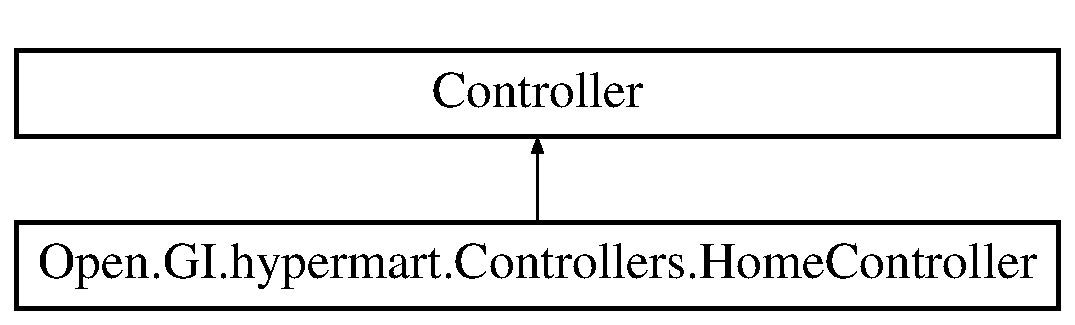
\includegraphics[height=2.000000cm]{class_open_1_1_g_i_1_1hypermart_1_1_controllers_1_1_home_controller}
\end{center}
\end{figure}
\subsection*{Public Member Functions}
\begin{DoxyCompactItemize}
\item 
Action\+Result \hyperlink{class_open_1_1_g_i_1_1hypermart_1_1_controllers_1_1_home_controller_a18ad180258caf702a7cfe51c16bf5558}{Index} ()
\begin{DoxyCompactList}\small\item\em Indexes this instance. \end{DoxyCompactList}\item 
Action\+Result \hyperlink{class_open_1_1_g_i_1_1hypermart_1_1_controllers_1_1_home_controller_a6d90d2a8ae2ce9f7c9ec38b175847e6f}{About} ()
\begin{DoxyCompactList}\small\item\em Abouts this instance. \end{DoxyCompactList}\item 
Action\+Result \hyperlink{class_open_1_1_g_i_1_1hypermart_1_1_controllers_1_1_home_controller_a758666761af826c9091b8a8655eb5e18}{Contact} ()
\begin{DoxyCompactList}\small\item\em Contacts this instance. \end{DoxyCompactList}\end{DoxyCompactItemize}


\subsection{Detailed Description}
A\+S\+P.\+N\+E\+T M\+V\+C Home Controller 

\begin{DoxySeeAlso}{See also}
System.\+Web.\+Mvc.\+Controller


\end{DoxySeeAlso}


Definition at line 13 of file Home\+Controller.\+cs.



\subsection{Member Function Documentation}
\hypertarget{class_open_1_1_g_i_1_1hypermart_1_1_controllers_1_1_home_controller_a6d90d2a8ae2ce9f7c9ec38b175847e6f}{}\index{Open\+::\+G\+I\+::hypermart\+::\+Controllers\+::\+Home\+Controller@{Open\+::\+G\+I\+::hypermart\+::\+Controllers\+::\+Home\+Controller}!About@{About}}
\index{About@{About}!Open\+::\+G\+I\+::hypermart\+::\+Controllers\+::\+Home\+Controller@{Open\+::\+G\+I\+::hypermart\+::\+Controllers\+::\+Home\+Controller}}
\subsubsection[{About()}]{\setlength{\rightskip}{0pt plus 5cm}Action\+Result Open.\+G\+I.\+hypermart.\+Controllers.\+Home\+Controller.\+About (
\begin{DoxyParamCaption}
{}
\end{DoxyParamCaption}
)}\label{class_open_1_1_g_i_1_1hypermart_1_1_controllers_1_1_home_controller_a6d90d2a8ae2ce9f7c9ec38b175847e6f}


Abouts this instance. 

\begin{DoxyReturn}{Returns}

\end{DoxyReturn}


Definition at line 28 of file Home\+Controller.\+cs.

\hypertarget{class_open_1_1_g_i_1_1hypermart_1_1_controllers_1_1_home_controller_a758666761af826c9091b8a8655eb5e18}{}\index{Open\+::\+G\+I\+::hypermart\+::\+Controllers\+::\+Home\+Controller@{Open\+::\+G\+I\+::hypermart\+::\+Controllers\+::\+Home\+Controller}!Contact@{Contact}}
\index{Contact@{Contact}!Open\+::\+G\+I\+::hypermart\+::\+Controllers\+::\+Home\+Controller@{Open\+::\+G\+I\+::hypermart\+::\+Controllers\+::\+Home\+Controller}}
\subsubsection[{Contact()}]{\setlength{\rightskip}{0pt plus 5cm}Action\+Result Open.\+G\+I.\+hypermart.\+Controllers.\+Home\+Controller.\+Contact (
\begin{DoxyParamCaption}
{}
\end{DoxyParamCaption}
)}\label{class_open_1_1_g_i_1_1hypermart_1_1_controllers_1_1_home_controller_a758666761af826c9091b8a8655eb5e18}


Contacts this instance. 

\begin{DoxyReturn}{Returns}

\end{DoxyReturn}


Definition at line 39 of file Home\+Controller.\+cs.

\hypertarget{class_open_1_1_g_i_1_1hypermart_1_1_controllers_1_1_home_controller_a18ad180258caf702a7cfe51c16bf5558}{}\index{Open\+::\+G\+I\+::hypermart\+::\+Controllers\+::\+Home\+Controller@{Open\+::\+G\+I\+::hypermart\+::\+Controllers\+::\+Home\+Controller}!Index@{Index}}
\index{Index@{Index}!Open\+::\+G\+I\+::hypermart\+::\+Controllers\+::\+Home\+Controller@{Open\+::\+G\+I\+::hypermart\+::\+Controllers\+::\+Home\+Controller}}
\subsubsection[{Index()}]{\setlength{\rightskip}{0pt plus 5cm}Action\+Result Open.\+G\+I.\+hypermart.\+Controllers.\+Home\+Controller.\+Index (
\begin{DoxyParamCaption}
{}
\end{DoxyParamCaption}
)}\label{class_open_1_1_g_i_1_1hypermart_1_1_controllers_1_1_home_controller_a18ad180258caf702a7cfe51c16bf5558}


Indexes this instance. 

\begin{DoxyReturn}{Returns}

\end{DoxyReturn}


Definition at line 19 of file Home\+Controller.\+cs.



The documentation for this class was generated from the following file\+:\begin{DoxyCompactItemize}
\item 
C\+:/\+Projects/\+App-\/\+Utility-\/\+Store/\+Open.\+G\+I.\+hypermart/\+Controllers/\hyperlink{_home_controller_8cs}{Home\+Controller.\+cs}\end{DoxyCompactItemize}

\hypertarget{class_open_1_1_g_i_1_1hypermart_1_1_d_a_l_1_1_hypermart_context}{}\section{Open.\+G\+I.\+hypermart.\+D\+A\+L.\+Hypermart\+Context Class Reference}
\label{class_open_1_1_g_i_1_1hypermart_1_1_d_a_l_1_1_hypermart_context}\index{Open.\+G\+I.\+hypermart.\+D\+A\+L.\+Hypermart\+Context@{Open.\+G\+I.\+hypermart.\+D\+A\+L.\+Hypermart\+Context}}


Hypermart Context  


Inheritance diagram for Open.\+G\+I.\+hypermart.\+D\+A\+L.\+Hypermart\+Context\+:\begin{figure}[H]
\begin{center}
\leavevmode
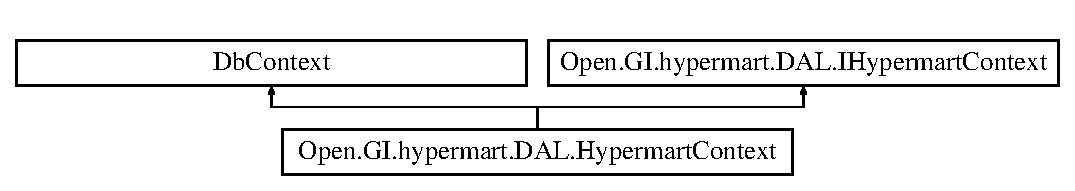
\includegraphics[height=2.000000cm]{class_open_1_1_g_i_1_1hypermart_1_1_d_a_l_1_1_hypermart_context}
\end{center}
\end{figure}
\subsection*{Public Member Functions}
\begin{DoxyCompactItemize}
\item 
\hyperlink{class_open_1_1_g_i_1_1hypermart_1_1_d_a_l_1_1_hypermart_context_a3bcbe3fbf08e41a8b384326b606a7327}{Hypermart\+Context} ()
\begin{DoxyCompactList}\small\item\em Initializes a new instance of the \hyperlink{class_open_1_1_g_i_1_1hypermart_1_1_d_a_l_1_1_hypermart_context}{Hypermart\+Context} class. \end{DoxyCompactList}\item 
new void \hyperlink{class_open_1_1_g_i_1_1hypermart_1_1_d_a_l_1_1_hypermart_context_a30d97828a1a45fcdf9b51cadb10029a4}{Save\+Changes} ()
\begin{DoxyCompactList}\small\item\em In a D\+B Context object, this should save all changes made in this context to the underlying database \end{DoxyCompactList}\end{DoxyCompactItemize}
\subsection*{Protected Member Functions}
\begin{DoxyCompactItemize}
\item 
override void \hyperlink{class_open_1_1_g_i_1_1hypermart_1_1_d_a_l_1_1_hypermart_context_a1a255d0b197dd90f76233146c608a0f1}{On\+Model\+Creating} (Db\+Model\+Builder model\+Builder)
\begin{DoxyCompactList}\small\item\em This method is called when the model for a derived context has been initialized, but before the model has been locked down and used to initialize the context. The default implementation of this method does nothing, but it can be overridden in a derived class such that the model can be further configured before it is locked down. \end{DoxyCompactList}\end{DoxyCompactItemize}
\subsection*{Properties}
\begin{DoxyCompactItemize}
\item 
virtual Db\+Set$<$ \hyperlink{class_open_1_1_g_i_1_1hypermart_1_1_models_1_1_file}{File} $>$ \hyperlink{class_open_1_1_g_i_1_1hypermart_1_1_d_a_l_1_1_hypermart_context_aa42b145ebbfe133c3bc2beddfb23de36}{Files}\hspace{0.3cm}{\ttfamily  \mbox{[}get, set\mbox{]}}
\begin{DoxyCompactList}\small\item\em Gets or sets the files. \end{DoxyCompactList}\item 
virtual Db\+Set$<$ \hyperlink{class_open_1_1_g_i_1_1hypermart_1_1_models_1_1_platform}{Platform} $>$ \hyperlink{class_open_1_1_g_i_1_1hypermart_1_1_d_a_l_1_1_hypermart_context_aff4be9e14ae1b0224c5a7b780050222f}{Platforms}\hspace{0.3cm}{\ttfamily  \mbox{[}get, set\mbox{]}}
\begin{DoxyCompactList}\small\item\em Gets or sets the platforms. \end{DoxyCompactList}\item 
virtual Db\+Set$<$ \hyperlink{class_open_1_1_g_i_1_1hypermart_1_1_models_1_1_product}{Product} $>$ \hyperlink{class_open_1_1_g_i_1_1hypermart_1_1_d_a_l_1_1_hypermart_context_a2673d17b8a620d2f9f11f44edd5d86ef}{Products}\hspace{0.3cm}{\ttfamily  \mbox{[}get, set\mbox{]}}
\begin{DoxyCompactList}\small\item\em Gets or sets the products. \end{DoxyCompactList}\item 
virtual Db\+Set$<$ \hyperlink{class_open_1_1_g_i_1_1hypermart_1_1_models_1_1_screenshot}{Screenshot} $>$ \hyperlink{class_open_1_1_g_i_1_1hypermart_1_1_d_a_l_1_1_hypermart_context_a267136fa00e08f78b49a0a888e548bef}{Screenshots}\hspace{0.3cm}{\ttfamily  \mbox{[}get, set\mbox{]}}
\begin{DoxyCompactList}\small\item\em Gets or sets the screenshots. \end{DoxyCompactList}\end{DoxyCompactItemize}


\subsection{Detailed Description}
Hypermart Context 

\begin{DoxySeeAlso}{See also}
System.\+Data.\+Entity.\+Db\+Context, \hyperlink{interface_open_1_1_g_i_1_1hypermart_1_1_d_a_l_1_1_i_hypermart_context}{Open.\+G\+I.\+hypermart.\+D\+A\+L.\+I\+Hypermart\+Context}


\end{DoxySeeAlso}


Definition at line 14 of file Hypermart\+Context.\+cs.



\subsection{Constructor \& Destructor Documentation}
\hypertarget{class_open_1_1_g_i_1_1hypermart_1_1_d_a_l_1_1_hypermart_context_a3bcbe3fbf08e41a8b384326b606a7327}{}\index{Open\+::\+G\+I\+::hypermart\+::\+D\+A\+L\+::\+Hypermart\+Context@{Open\+::\+G\+I\+::hypermart\+::\+D\+A\+L\+::\+Hypermart\+Context}!Hypermart\+Context@{Hypermart\+Context}}
\index{Hypermart\+Context@{Hypermart\+Context}!Open\+::\+G\+I\+::hypermart\+::\+D\+A\+L\+::\+Hypermart\+Context@{Open\+::\+G\+I\+::hypermart\+::\+D\+A\+L\+::\+Hypermart\+Context}}
\subsubsection[{Hypermart\+Context()}]{\setlength{\rightskip}{0pt plus 5cm}Open.\+G\+I.\+hypermart.\+D\+A\+L.\+Hypermart\+Context.\+Hypermart\+Context (
\begin{DoxyParamCaption}
{}
\end{DoxyParamCaption}
)}\label{class_open_1_1_g_i_1_1hypermart_1_1_d_a_l_1_1_hypermart_context_a3bcbe3fbf08e41a8b384326b606a7327}


Initializes a new instance of the \hyperlink{class_open_1_1_g_i_1_1hypermart_1_1_d_a_l_1_1_hypermart_context}{Hypermart\+Context} class. 



Definition at line 19 of file Hypermart\+Context.\+cs.



\subsection{Member Function Documentation}
\hypertarget{class_open_1_1_g_i_1_1hypermart_1_1_d_a_l_1_1_hypermart_context_a1a255d0b197dd90f76233146c608a0f1}{}\index{Open\+::\+G\+I\+::hypermart\+::\+D\+A\+L\+::\+Hypermart\+Context@{Open\+::\+G\+I\+::hypermart\+::\+D\+A\+L\+::\+Hypermart\+Context}!On\+Model\+Creating@{On\+Model\+Creating}}
\index{On\+Model\+Creating@{On\+Model\+Creating}!Open\+::\+G\+I\+::hypermart\+::\+D\+A\+L\+::\+Hypermart\+Context@{Open\+::\+G\+I\+::hypermart\+::\+D\+A\+L\+::\+Hypermart\+Context}}
\subsubsection[{On\+Model\+Creating(\+Db\+Model\+Builder model\+Builder)}]{\setlength{\rightskip}{0pt plus 5cm}override void Open.\+G\+I.\+hypermart.\+D\+A\+L.\+Hypermart\+Context.\+On\+Model\+Creating (
\begin{DoxyParamCaption}
\item[{Db\+Model\+Builder}]{model\+Builder}
\end{DoxyParamCaption}
)\hspace{0.3cm}{\ttfamily [protected]}}\label{class_open_1_1_g_i_1_1hypermart_1_1_d_a_l_1_1_hypermart_context_a1a255d0b197dd90f76233146c608a0f1}


This method is called when the model for a derived context has been initialized, but before the model has been locked down and used to initialize the context. The default implementation of this method does nothing, but it can be overridden in a derived class such that the model can be further configured before it is locked down. 


\begin{DoxyParams}{Parameters}
{\em model\+Builder} & The builder that defines the model for the context being created.\\
\hline
\end{DoxyParams}


Typically, this method is called only once when the first instance of a derived context is created. The model for that context is then cached and is for all further instances of the context in the app domain. This caching can be disabled by setting the Model\+Caching property on the given Model\+Buidler, but note that this can seriously degrade performance. More control over caching is provided through use of the Db\+Model\+Builder and Db\+Context\+Factory classes directly. 

Definition at line 67 of file Hypermart\+Context.\+cs.

\hypertarget{class_open_1_1_g_i_1_1hypermart_1_1_d_a_l_1_1_hypermart_context_a30d97828a1a45fcdf9b51cadb10029a4}{}\index{Open\+::\+G\+I\+::hypermart\+::\+D\+A\+L\+::\+Hypermart\+Context@{Open\+::\+G\+I\+::hypermart\+::\+D\+A\+L\+::\+Hypermart\+Context}!Save\+Changes@{Save\+Changes}}
\index{Save\+Changes@{Save\+Changes}!Open\+::\+G\+I\+::hypermart\+::\+D\+A\+L\+::\+Hypermart\+Context@{Open\+::\+G\+I\+::hypermart\+::\+D\+A\+L\+::\+Hypermart\+Context}}
\subsubsection[{Save\+Changes()}]{\setlength{\rightskip}{0pt plus 5cm}new void Open.\+G\+I.\+hypermart.\+D\+A\+L.\+Hypermart\+Context.\+Save\+Changes (
\begin{DoxyParamCaption}
{}
\end{DoxyParamCaption}
)}\label{class_open_1_1_g_i_1_1hypermart_1_1_d_a_l_1_1_hypermart_context_a30d97828a1a45fcdf9b51cadb10029a4}


In a D\+B Context object, this should save all changes made in this context to the underlying database 



Implements \hyperlink{interface_open_1_1_g_i_1_1hypermart_1_1_d_a_l_1_1_i_hypermart_context_aacc5015260d97950f2a10d7673873304}{Open.\+G\+I.\+hypermart.\+D\+A\+L.\+I\+Hypermart\+Context}.



Definition at line 84 of file Hypermart\+Context.\+cs.



\subsection{Property Documentation}
\hypertarget{class_open_1_1_g_i_1_1hypermart_1_1_d_a_l_1_1_hypermart_context_aa42b145ebbfe133c3bc2beddfb23de36}{}\index{Open\+::\+G\+I\+::hypermart\+::\+D\+A\+L\+::\+Hypermart\+Context@{Open\+::\+G\+I\+::hypermart\+::\+D\+A\+L\+::\+Hypermart\+Context}!Files@{Files}}
\index{Files@{Files}!Open\+::\+G\+I\+::hypermart\+::\+D\+A\+L\+::\+Hypermart\+Context@{Open\+::\+G\+I\+::hypermart\+::\+D\+A\+L\+::\+Hypermart\+Context}}
\subsubsection[{Files}]{\setlength{\rightskip}{0pt plus 5cm}virtual Db\+Set$<${\bf File}$>$ Open.\+G\+I.\+hypermart.\+D\+A\+L.\+Hypermart\+Context.\+Files\hspace{0.3cm}{\ttfamily [get]}, {\ttfamily [set]}}\label{class_open_1_1_g_i_1_1hypermart_1_1_d_a_l_1_1_hypermart_context_aa42b145ebbfe133c3bc2beddfb23de36}


Gets or sets the files. 

The files. 

Definition at line 29 of file Hypermart\+Context.\+cs.

\hypertarget{class_open_1_1_g_i_1_1hypermart_1_1_d_a_l_1_1_hypermart_context_aff4be9e14ae1b0224c5a7b780050222f}{}\index{Open\+::\+G\+I\+::hypermart\+::\+D\+A\+L\+::\+Hypermart\+Context@{Open\+::\+G\+I\+::hypermart\+::\+D\+A\+L\+::\+Hypermart\+Context}!Platforms@{Platforms}}
\index{Platforms@{Platforms}!Open\+::\+G\+I\+::hypermart\+::\+D\+A\+L\+::\+Hypermart\+Context@{Open\+::\+G\+I\+::hypermart\+::\+D\+A\+L\+::\+Hypermart\+Context}}
\subsubsection[{Platforms}]{\setlength{\rightskip}{0pt plus 5cm}virtual Db\+Set$<${\bf Platform}$>$ Open.\+G\+I.\+hypermart.\+D\+A\+L.\+Hypermart\+Context.\+Platforms\hspace{0.3cm}{\ttfamily [get]}, {\ttfamily [set]}}\label{class_open_1_1_g_i_1_1hypermart_1_1_d_a_l_1_1_hypermart_context_aff4be9e14ae1b0224c5a7b780050222f}


Gets or sets the platforms. 

The platforms. 

Definition at line 36 of file Hypermart\+Context.\+cs.

\hypertarget{class_open_1_1_g_i_1_1hypermart_1_1_d_a_l_1_1_hypermart_context_a2673d17b8a620d2f9f11f44edd5d86ef}{}\index{Open\+::\+G\+I\+::hypermart\+::\+D\+A\+L\+::\+Hypermart\+Context@{Open\+::\+G\+I\+::hypermart\+::\+D\+A\+L\+::\+Hypermart\+Context}!Products@{Products}}
\index{Products@{Products}!Open\+::\+G\+I\+::hypermart\+::\+D\+A\+L\+::\+Hypermart\+Context@{Open\+::\+G\+I\+::hypermart\+::\+D\+A\+L\+::\+Hypermart\+Context}}
\subsubsection[{Products}]{\setlength{\rightskip}{0pt plus 5cm}virtual Db\+Set$<${\bf Product}$>$ Open.\+G\+I.\+hypermart.\+D\+A\+L.\+Hypermart\+Context.\+Products\hspace{0.3cm}{\ttfamily [get]}, {\ttfamily [set]}}\label{class_open_1_1_g_i_1_1hypermart_1_1_d_a_l_1_1_hypermart_context_a2673d17b8a620d2f9f11f44edd5d86ef}


Gets or sets the products. 

The products. 

Definition at line 43 of file Hypermart\+Context.\+cs.

\hypertarget{class_open_1_1_g_i_1_1hypermart_1_1_d_a_l_1_1_hypermart_context_a267136fa00e08f78b49a0a888e548bef}{}\index{Open\+::\+G\+I\+::hypermart\+::\+D\+A\+L\+::\+Hypermart\+Context@{Open\+::\+G\+I\+::hypermart\+::\+D\+A\+L\+::\+Hypermart\+Context}!Screenshots@{Screenshots}}
\index{Screenshots@{Screenshots}!Open\+::\+G\+I\+::hypermart\+::\+D\+A\+L\+::\+Hypermart\+Context@{Open\+::\+G\+I\+::hypermart\+::\+D\+A\+L\+::\+Hypermart\+Context}}
\subsubsection[{Screenshots}]{\setlength{\rightskip}{0pt plus 5cm}virtual Db\+Set$<${\bf Screenshot}$>$ Open.\+G\+I.\+hypermart.\+D\+A\+L.\+Hypermart\+Context.\+Screenshots\hspace{0.3cm}{\ttfamily [get]}, {\ttfamily [set]}}\label{class_open_1_1_g_i_1_1hypermart_1_1_d_a_l_1_1_hypermart_context_a267136fa00e08f78b49a0a888e548bef}


Gets or sets the screenshots. 

The screenshots. 

Definition at line 50 of file Hypermart\+Context.\+cs.



The documentation for this class was generated from the following file\+:\begin{DoxyCompactItemize}
\item 
C\+:/\+Projects/\+App-\/\+Utility-\/\+Store/\+Open.\+G\+I.\+hypermart/\+D\+A\+L/\hyperlink{_hypermart_context_8cs}{Hypermart\+Context.\+cs}\end{DoxyCompactItemize}

\hypertarget{class_open_1_1_g_i_1_1hypermart_1_1_d_a_l_1_1_hypermart_initializer}{}\section{Open.\+G\+I.\+hypermart.\+D\+A\+L.\+Hypermart\+Initializer Class Reference}
\label{class_open_1_1_g_i_1_1hypermart_1_1_d_a_l_1_1_hypermart_initializer}\index{Open.\+G\+I.\+hypermart.\+D\+A\+L.\+Hypermart\+Initializer@{Open.\+G\+I.\+hypermart.\+D\+A\+L.\+Hypermart\+Initializer}}


Hypermart Initializer  


Inheritance diagram for Open.\+G\+I.\+hypermart.\+D\+A\+L.\+Hypermart\+Initializer\+:\begin{figure}[H]
\begin{center}
\leavevmode
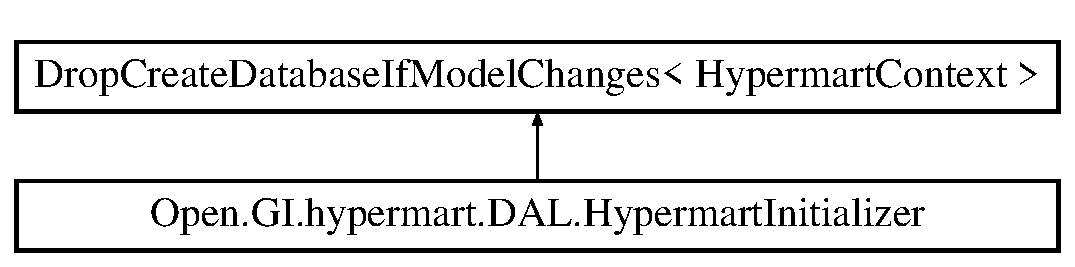
\includegraphics[height=2.000000cm]{class_open_1_1_g_i_1_1hypermart_1_1_d_a_l_1_1_hypermart_initializer}
\end{center}
\end{figure}
\subsection*{Protected Member Functions}
\begin{DoxyCompactItemize}
\item 
override void \hyperlink{class_open_1_1_g_i_1_1hypermart_1_1_d_a_l_1_1_hypermart_initializer_a2e19732fa6f8db0a6b72049415947016}{Seed} (\hyperlink{class_open_1_1_g_i_1_1hypermart_1_1_d_a_l_1_1_hypermart_context}{Hypermart\+Context} context)
\begin{DoxyCompactList}\small\item\em Seeds the database with content. \end{DoxyCompactList}\end{DoxyCompactItemize}


\subsection{Detailed Description}
Hypermart Initializer 



Definition at line 15 of file Hypermart\+Initializer.\+cs.



\subsection{Member Function Documentation}
\hypertarget{class_open_1_1_g_i_1_1hypermart_1_1_d_a_l_1_1_hypermart_initializer_a2e19732fa6f8db0a6b72049415947016}{}\index{Open\+::\+G\+I\+::hypermart\+::\+D\+A\+L\+::\+Hypermart\+Initializer@{Open\+::\+G\+I\+::hypermart\+::\+D\+A\+L\+::\+Hypermart\+Initializer}!Seed@{Seed}}
\index{Seed@{Seed}!Open\+::\+G\+I\+::hypermart\+::\+D\+A\+L\+::\+Hypermart\+Initializer@{Open\+::\+G\+I\+::hypermart\+::\+D\+A\+L\+::\+Hypermart\+Initializer}}
\subsubsection[{Seed(\+Hypermart\+Context context)}]{\setlength{\rightskip}{0pt plus 5cm}override void Open.\+G\+I.\+hypermart.\+D\+A\+L.\+Hypermart\+Initializer.\+Seed (
\begin{DoxyParamCaption}
\item[{{\bf Hypermart\+Context}}]{context}
\end{DoxyParamCaption}
)\hspace{0.3cm}{\ttfamily [protected]}}\label{class_open_1_1_g_i_1_1hypermart_1_1_d_a_l_1_1_hypermart_initializer_a2e19732fa6f8db0a6b72049415947016}


Seeds the database with content. 


\begin{DoxyParams}{Parameters}
{\em context} & The context.\\
\hline
\end{DoxyParams}


Definition at line 21 of file Hypermart\+Initializer.\+cs.



The documentation for this class was generated from the following file\+:\begin{DoxyCompactItemize}
\item 
C\+:/\+Projects/\+App-\/\+Utility-\/\+Store/\+Open.\+G\+I.\+hypermart/\+D\+A\+L/\hyperlink{_hypermart_initializer_8cs}{Hypermart\+Initializer.\+cs}\end{DoxyCompactItemize}

\section{Open.\+G\+I.\+hypermart.\+D\+A\+L.\+I\+Hypermart\+Context Interface Reference}
\label{interface_open_1_1_g_i_1_1hypermart_1_1_d_a_l_1_1_i_hypermart_context}\index{Open.\+G\+I.\+hypermart.\+D\+A\+L.\+I\+Hypermart\+Context@{Open.\+G\+I.\+hypermart.\+D\+A\+L.\+I\+Hypermart\+Context}}


Interface describing the functionality of the Database Context  


Inheritance diagram for Open.\+G\+I.\+hypermart.\+D\+A\+L.\+I\+Hypermart\+Context\+:\begin{figure}[H]
\begin{center}
\leavevmode
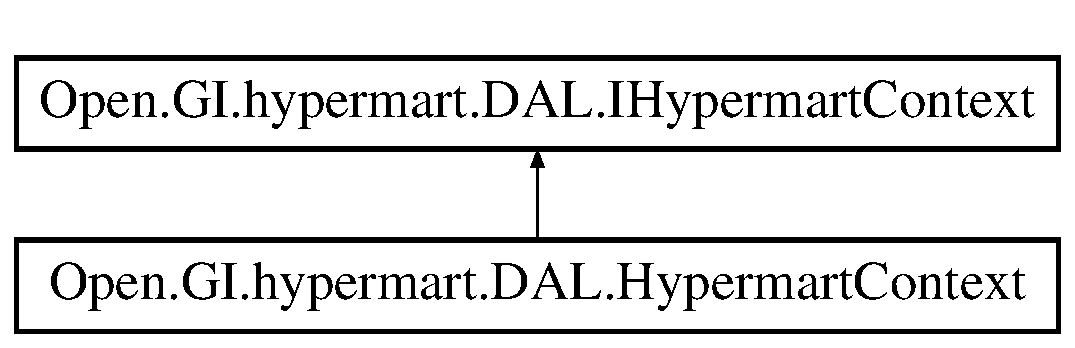
\includegraphics[height=3.000000cm]{interface_open_1_1_g_i_1_1hypermart_1_1_d_a_l_1_1_i_hypermart_context}
\end{center}
\end{figure}
\subsection*{Public Member Functions}
\begin{DoxyCompactItemize}
\item 
void \textbf{ Save\+Changes} ()
\begin{DoxyCompactList}\small\item\em In a DB Context object, this should save all changes made in this context to the underlying database \end{DoxyCompactList}\end{DoxyCompactItemize}
\subsection*{Properties}
\begin{DoxyCompactItemize}
\item 
System.\+Data.\+Entity.\+I\+Db\+Set$<$ \textbf{ Open.\+G\+I.\+hypermart.\+Models.\+File} $>$ \textbf{ Files}\hspace{0.3cm}{\ttfamily  [get, set]}
\begin{DoxyCompactList}\small\item\em Gets or sets the files. \end{DoxyCompactList}\item 
System.\+Data.\+Entity.\+I\+Db\+Set$<$ \textbf{ Open.\+G\+I.\+hypermart.\+Models.\+Platform} $>$ \textbf{ Platforms}\hspace{0.3cm}{\ttfamily  [get, set]}
\begin{DoxyCompactList}\small\item\em Gets or sets the platforms. \end{DoxyCompactList}\item 
System.\+Data.\+Entity.\+I\+Db\+Set$<$ \textbf{ Open.\+G\+I.\+hypermart.\+Models.\+Product} $>$ \textbf{ Products}\hspace{0.3cm}{\ttfamily  [get, set]}
\begin{DoxyCompactList}\small\item\em Gets or sets the products. \end{DoxyCompactList}\item 
System.\+Data.\+Entity.\+I\+Db\+Set$<$ \textbf{ Open.\+G\+I.\+hypermart.\+Models.\+Screenshot} $>$ \textbf{ Screenshots}\hspace{0.3cm}{\ttfamily  [get, set]}
\begin{DoxyCompactList}\small\item\em Gets or sets the screenshots. \end{DoxyCompactList}\item 
System.\+Data.\+Entity.\+I\+Db\+Set$<$ \textbf{ Open.\+G\+I.\+hypermart.\+Models.\+Rating} $>$ \textbf{ Ratings}\hspace{0.3cm}{\ttfamily  [get, set]}
\begin{DoxyCompactList}\small\item\em Gets or sets the ratings. \end{DoxyCompactList}\end{DoxyCompactItemize}


\subsection{Detailed Description}
Interface describing the functionality of the Database Context 



Definition at line 9 of file I\+Hypermart\+Context.\+cs.



\subsection{Member Function Documentation}
\mbox{\label{interface_open_1_1_g_i_1_1hypermart_1_1_d_a_l_1_1_i_hypermart_context_aacc5015260d97950f2a10d7673873304}} 
\index{Open\+::\+G\+I\+::hypermart\+::\+D\+A\+L\+::\+I\+Hypermart\+Context@{Open\+::\+G\+I\+::hypermart\+::\+D\+A\+L\+::\+I\+Hypermart\+Context}!Save\+Changes@{Save\+Changes}}
\index{Save\+Changes@{Save\+Changes}!Open\+::\+G\+I\+::hypermart\+::\+D\+A\+L\+::\+I\+Hypermart\+Context@{Open\+::\+G\+I\+::hypermart\+::\+D\+A\+L\+::\+I\+Hypermart\+Context}}
\subsubsection{Save\+Changes()}
{\footnotesize\ttfamily void Open.\+G\+I.\+hypermart.\+D\+A\+L.\+I\+Hypermart\+Context.\+Save\+Changes (\begin{DoxyParamCaption}{ }\end{DoxyParamCaption})}



In a DB Context object, this should save all changes made in this context to the underlying database 



Implemented in \textbf{ Open.\+G\+I.\+hypermart.\+D\+A\+L.\+Hypermart\+Context} \doxyref{}{p.}{class_open_1_1_g_i_1_1hypermart_1_1_d_a_l_1_1_hypermart_context_a53edb75fbc2507fc97eaf26e36d92f42}.



\subsection{Property Documentation}
\mbox{\label{interface_open_1_1_g_i_1_1hypermart_1_1_d_a_l_1_1_i_hypermart_context_a43675ffb78127ee6af56534c51d593c5}} 
\index{Open\+::\+G\+I\+::hypermart\+::\+D\+A\+L\+::\+I\+Hypermart\+Context@{Open\+::\+G\+I\+::hypermart\+::\+D\+A\+L\+::\+I\+Hypermart\+Context}!Files@{Files}}
\index{Files@{Files}!Open\+::\+G\+I\+::hypermart\+::\+D\+A\+L\+::\+I\+Hypermart\+Context@{Open\+::\+G\+I\+::hypermart\+::\+D\+A\+L\+::\+I\+Hypermart\+Context}}
\subsubsection{Files}
{\footnotesize\ttfamily System.\+Data.\+Entity.\+I\+Db\+Set$<$\textbf{ Open.\+G\+I.\+hypermart.\+Models.\+File}$>$ Open.\+G\+I.\+hypermart.\+D\+A\+L.\+I\+Hypermart\+Context.\+Files\hspace{0.3cm}{\ttfamily [get]}, {\ttfamily [set]}}



Gets or sets the files. 

The files. 

Definition at line 17 of file I\+Hypermart\+Context.\+cs.

\mbox{\label{interface_open_1_1_g_i_1_1hypermart_1_1_d_a_l_1_1_i_hypermart_context_a555845fae4537e83a55b431d87b6642e}} 
\index{Open\+::\+G\+I\+::hypermart\+::\+D\+A\+L\+::\+I\+Hypermart\+Context@{Open\+::\+G\+I\+::hypermart\+::\+D\+A\+L\+::\+I\+Hypermart\+Context}!Platforms@{Platforms}}
\index{Platforms@{Platforms}!Open\+::\+G\+I\+::hypermart\+::\+D\+A\+L\+::\+I\+Hypermart\+Context@{Open\+::\+G\+I\+::hypermart\+::\+D\+A\+L\+::\+I\+Hypermart\+Context}}
\subsubsection{Platforms}
{\footnotesize\ttfamily System.\+Data.\+Entity.\+I\+Db\+Set$<$\textbf{ Open.\+G\+I.\+hypermart.\+Models.\+Platform}$>$ Open.\+G\+I.\+hypermart.\+D\+A\+L.\+I\+Hypermart\+Context.\+Platforms\hspace{0.3cm}{\ttfamily [get]}, {\ttfamily [set]}}



Gets or sets the platforms. 

The platforms. 

Definition at line 24 of file I\+Hypermart\+Context.\+cs.

\mbox{\label{interface_open_1_1_g_i_1_1hypermart_1_1_d_a_l_1_1_i_hypermart_context_addebf65ed282146ad46149f0a4575ec7}} 
\index{Open\+::\+G\+I\+::hypermart\+::\+D\+A\+L\+::\+I\+Hypermart\+Context@{Open\+::\+G\+I\+::hypermart\+::\+D\+A\+L\+::\+I\+Hypermart\+Context}!Products@{Products}}
\index{Products@{Products}!Open\+::\+G\+I\+::hypermart\+::\+D\+A\+L\+::\+I\+Hypermart\+Context@{Open\+::\+G\+I\+::hypermart\+::\+D\+A\+L\+::\+I\+Hypermart\+Context}}
\subsubsection{Products}
{\footnotesize\ttfamily System.\+Data.\+Entity.\+I\+Db\+Set$<$\textbf{ Open.\+G\+I.\+hypermart.\+Models.\+Product}$>$ Open.\+G\+I.\+hypermart.\+D\+A\+L.\+I\+Hypermart\+Context.\+Products\hspace{0.3cm}{\ttfamily [get]}, {\ttfamily [set]}}



Gets or sets the products. 

The products. 

Definition at line 31 of file I\+Hypermart\+Context.\+cs.

\mbox{\label{interface_open_1_1_g_i_1_1hypermart_1_1_d_a_l_1_1_i_hypermart_context_a4e1ab8903a144091a90920c6e3e62d32}} 
\index{Open\+::\+G\+I\+::hypermart\+::\+D\+A\+L\+::\+I\+Hypermart\+Context@{Open\+::\+G\+I\+::hypermart\+::\+D\+A\+L\+::\+I\+Hypermart\+Context}!Ratings@{Ratings}}
\index{Ratings@{Ratings}!Open\+::\+G\+I\+::hypermart\+::\+D\+A\+L\+::\+I\+Hypermart\+Context@{Open\+::\+G\+I\+::hypermart\+::\+D\+A\+L\+::\+I\+Hypermart\+Context}}
\subsubsection{Ratings}
{\footnotesize\ttfamily System.\+Data.\+Entity.\+I\+Db\+Set$<$\textbf{ Open.\+G\+I.\+hypermart.\+Models.\+Rating}$>$ Open.\+G\+I.\+hypermart.\+D\+A\+L.\+I\+Hypermart\+Context.\+Ratings\hspace{0.3cm}{\ttfamily [get]}, {\ttfamily [set]}}



Gets or sets the ratings. 

The ratings. 

Definition at line 45 of file I\+Hypermart\+Context.\+cs.

\mbox{\label{interface_open_1_1_g_i_1_1hypermart_1_1_d_a_l_1_1_i_hypermart_context_ab60981916a8ecd6e871be2f4cb699b19}} 
\index{Open\+::\+G\+I\+::hypermart\+::\+D\+A\+L\+::\+I\+Hypermart\+Context@{Open\+::\+G\+I\+::hypermart\+::\+D\+A\+L\+::\+I\+Hypermart\+Context}!Screenshots@{Screenshots}}
\index{Screenshots@{Screenshots}!Open\+::\+G\+I\+::hypermart\+::\+D\+A\+L\+::\+I\+Hypermart\+Context@{Open\+::\+G\+I\+::hypermart\+::\+D\+A\+L\+::\+I\+Hypermart\+Context}}
\subsubsection{Screenshots}
{\footnotesize\ttfamily System.\+Data.\+Entity.\+I\+Db\+Set$<$\textbf{ Open.\+G\+I.\+hypermart.\+Models.\+Screenshot}$>$ Open.\+G\+I.\+hypermart.\+D\+A\+L.\+I\+Hypermart\+Context.\+Screenshots\hspace{0.3cm}{\ttfamily [get]}, {\ttfamily [set]}}



Gets or sets the screenshots. 

The screenshots. 

Definition at line 38 of file I\+Hypermart\+Context.\+cs.



The documentation for this interface was generated from the following file\+:\begin{DoxyCompactItemize}
\item 
C\+:/\+Projects/\+App-\/\+Utility-\/\+Store/\+Open.\+G\+I.\+hypermart/\+D\+A\+L/\textbf{ I\+Hypermart\+Context.\+cs}\end{DoxyCompactItemize}

\hypertarget{class_open_1_1_g_i_1_1hypermart_1_1_areas_1_1_help_page_1_1_image_sample}{}\section{Open.\+G\+I.\+hypermart.\+Areas.\+Help\+Page.\+Image\+Sample Class Reference}
\label{class_open_1_1_g_i_1_1hypermart_1_1_areas_1_1_help_page_1_1_image_sample}\index{Open.\+G\+I.\+hypermart.\+Areas.\+Help\+Page.\+Image\+Sample@{Open.\+G\+I.\+hypermart.\+Areas.\+Help\+Page.\+Image\+Sample}}


This represents an image sample on the help page. There\textquotesingle{}s a display template named \hyperlink{class_open_1_1_g_i_1_1hypermart_1_1_areas_1_1_help_page_1_1_image_sample}{Image\+Sample} associated with this class.  


\subsection*{Public Member Functions}
\begin{DoxyCompactItemize}
\item 
\hyperlink{class_open_1_1_g_i_1_1hypermart_1_1_areas_1_1_help_page_1_1_image_sample_a3570ac8793e478a72e64041784f39120}{Image\+Sample} (string src)
\begin{DoxyCompactList}\small\item\em Initializes a new instance of the \hyperlink{class_open_1_1_g_i_1_1hypermart_1_1_areas_1_1_help_page_1_1_image_sample}{Image\+Sample} class. \end{DoxyCompactList}\item 
override bool \hyperlink{class_open_1_1_g_i_1_1hypermart_1_1_areas_1_1_help_page_1_1_image_sample_a51e16a01c4f9a5a568c82d1f2d093337}{Equals} (object obj)
\begin{DoxyCompactList}\small\item\em Determines whether the specified System.\+Object, is equal to this instance. \end{DoxyCompactList}\item 
override int \hyperlink{class_open_1_1_g_i_1_1hypermart_1_1_areas_1_1_help_page_1_1_image_sample_a3374507c967e37d7fcba28ec9481865b}{Get\+Hash\+Code} ()
\begin{DoxyCompactList}\small\item\em Returns a hash code for this instance. \end{DoxyCompactList}\item 
override string \hyperlink{class_open_1_1_g_i_1_1hypermart_1_1_areas_1_1_help_page_1_1_image_sample_a704782de956313701ca9e6e61692d433}{To\+String} ()
\begin{DoxyCompactList}\small\item\em Returns a System.\+String that represents this instance. \end{DoxyCompactList}\end{DoxyCompactItemize}
\subsection*{Properties}
\begin{DoxyCompactItemize}
\item 
string \hyperlink{class_open_1_1_g_i_1_1hypermart_1_1_areas_1_1_help_page_1_1_image_sample_a19a1c712823d2e81590e2be51f2e30fb}{Src}\hspace{0.3cm}{\ttfamily  \mbox{[}get\mbox{]}}
\end{DoxyCompactItemize}


\subsection{Detailed Description}
This represents an image sample on the help page. There\textquotesingle{}s a display template named \hyperlink{class_open_1_1_g_i_1_1hypermart_1_1_areas_1_1_help_page_1_1_image_sample}{Image\+Sample} associated with this class. 



\subsection{Constructor \& Destructor Documentation}
\hypertarget{class_open_1_1_g_i_1_1hypermart_1_1_areas_1_1_help_page_1_1_image_sample_a3570ac8793e478a72e64041784f39120}{}\label{class_open_1_1_g_i_1_1hypermart_1_1_areas_1_1_help_page_1_1_image_sample_a3570ac8793e478a72e64041784f39120} 
\index{Open\+::\+G\+I\+::hypermart\+::\+Areas\+::\+Help\+Page\+::\+Image\+Sample@{Open\+::\+G\+I\+::hypermart\+::\+Areas\+::\+Help\+Page\+::\+Image\+Sample}!Image\+Sample@{Image\+Sample}}
\index{Image\+Sample@{Image\+Sample}!Open\+::\+G\+I\+::hypermart\+::\+Areas\+::\+Help\+Page\+::\+Image\+Sample@{Open\+::\+G\+I\+::hypermart\+::\+Areas\+::\+Help\+Page\+::\+Image\+Sample}}
\subsubsection{\texorpdfstring{Image\+Sample()}{ImageSample()}}
{\footnotesize\ttfamily Open.\+G\+I.\+hypermart.\+Areas.\+Help\+Page.\+Image\+Sample.\+Image\+Sample (\begin{DoxyParamCaption}\item[{string}]{src }\end{DoxyParamCaption})}



Initializes a new instance of the \hyperlink{class_open_1_1_g_i_1_1hypermart_1_1_areas_1_1_help_page_1_1_image_sample}{Image\+Sample} class. 


\begin{DoxyParams}{Parameters}
{\em src} & The U\+RL of an image.\\
\hline
\end{DoxyParams}


\subsection{Member Function Documentation}
\hypertarget{class_open_1_1_g_i_1_1hypermart_1_1_areas_1_1_help_page_1_1_image_sample_a51e16a01c4f9a5a568c82d1f2d093337}{}\label{class_open_1_1_g_i_1_1hypermart_1_1_areas_1_1_help_page_1_1_image_sample_a51e16a01c4f9a5a568c82d1f2d093337} 
\index{Open\+::\+G\+I\+::hypermart\+::\+Areas\+::\+Help\+Page\+::\+Image\+Sample@{Open\+::\+G\+I\+::hypermart\+::\+Areas\+::\+Help\+Page\+::\+Image\+Sample}!Equals@{Equals}}
\index{Equals@{Equals}!Open\+::\+G\+I\+::hypermart\+::\+Areas\+::\+Help\+Page\+::\+Image\+Sample@{Open\+::\+G\+I\+::hypermart\+::\+Areas\+::\+Help\+Page\+::\+Image\+Sample}}
\subsubsection{\texorpdfstring{Equals()}{Equals()}}
{\footnotesize\ttfamily override bool Open.\+G\+I.\+hypermart.\+Areas.\+Help\+Page.\+Image\+Sample.\+Equals (\begin{DoxyParamCaption}\item[{object}]{obj }\end{DoxyParamCaption})}



Determines whether the specified System.\+Object, is equal to this instance. 


\begin{DoxyParams}{Parameters}
{\em obj} & The System.\+Object to compare with this instance.\\
\hline
\end{DoxyParams}
\begin{DoxyReturn}{Returns}
{\ttfamily true} if the specified System.\+Object is equal to this instance; otherwise, {\ttfamily false}. 
\end{DoxyReturn}
\hypertarget{class_open_1_1_g_i_1_1hypermart_1_1_areas_1_1_help_page_1_1_image_sample_a3374507c967e37d7fcba28ec9481865b}{}\label{class_open_1_1_g_i_1_1hypermart_1_1_areas_1_1_help_page_1_1_image_sample_a3374507c967e37d7fcba28ec9481865b} 
\index{Open\+::\+G\+I\+::hypermart\+::\+Areas\+::\+Help\+Page\+::\+Image\+Sample@{Open\+::\+G\+I\+::hypermart\+::\+Areas\+::\+Help\+Page\+::\+Image\+Sample}!Get\+Hash\+Code@{Get\+Hash\+Code}}
\index{Get\+Hash\+Code@{Get\+Hash\+Code}!Open\+::\+G\+I\+::hypermart\+::\+Areas\+::\+Help\+Page\+::\+Image\+Sample@{Open\+::\+G\+I\+::hypermart\+::\+Areas\+::\+Help\+Page\+::\+Image\+Sample}}
\subsubsection{\texorpdfstring{Get\+Hash\+Code()}{GetHashCode()}}
{\footnotesize\ttfamily override int Open.\+G\+I.\+hypermart.\+Areas.\+Help\+Page.\+Image\+Sample.\+Get\+Hash\+Code (\begin{DoxyParamCaption}{ }\end{DoxyParamCaption})}



Returns a hash code for this instance. 

\begin{DoxyReturn}{Returns}
A hash code for this instance, suitable for use in hashing algorithms and data structures like a hash table. 
\end{DoxyReturn}
\hypertarget{class_open_1_1_g_i_1_1hypermart_1_1_areas_1_1_help_page_1_1_image_sample_a704782de956313701ca9e6e61692d433}{}\label{class_open_1_1_g_i_1_1hypermart_1_1_areas_1_1_help_page_1_1_image_sample_a704782de956313701ca9e6e61692d433} 
\index{Open\+::\+G\+I\+::hypermart\+::\+Areas\+::\+Help\+Page\+::\+Image\+Sample@{Open\+::\+G\+I\+::hypermart\+::\+Areas\+::\+Help\+Page\+::\+Image\+Sample}!To\+String@{To\+String}}
\index{To\+String@{To\+String}!Open\+::\+G\+I\+::hypermart\+::\+Areas\+::\+Help\+Page\+::\+Image\+Sample@{Open\+::\+G\+I\+::hypermart\+::\+Areas\+::\+Help\+Page\+::\+Image\+Sample}}
\subsubsection{\texorpdfstring{To\+String()}{ToString()}}
{\footnotesize\ttfamily override string Open.\+G\+I.\+hypermart.\+Areas.\+Help\+Page.\+Image\+Sample.\+To\+String (\begin{DoxyParamCaption}{ }\end{DoxyParamCaption})}



Returns a System.\+String that represents this instance. 

\begin{DoxyReturn}{Returns}
A System.\+String that represents this instance. 
\end{DoxyReturn}


\subsection{Property Documentation}
\hypertarget{class_open_1_1_g_i_1_1hypermart_1_1_areas_1_1_help_page_1_1_image_sample_a19a1c712823d2e81590e2be51f2e30fb}{}\label{class_open_1_1_g_i_1_1hypermart_1_1_areas_1_1_help_page_1_1_image_sample_a19a1c712823d2e81590e2be51f2e30fb} 
\index{Open\+::\+G\+I\+::hypermart\+::\+Areas\+::\+Help\+Page\+::\+Image\+Sample@{Open\+::\+G\+I\+::hypermart\+::\+Areas\+::\+Help\+Page\+::\+Image\+Sample}!Src@{Src}}
\index{Src@{Src}!Open\+::\+G\+I\+::hypermart\+::\+Areas\+::\+Help\+Page\+::\+Image\+Sample@{Open\+::\+G\+I\+::hypermart\+::\+Areas\+::\+Help\+Page\+::\+Image\+Sample}}
\subsubsection{\texorpdfstring{Src}{Src}}
{\footnotesize\ttfamily string Open.\+G\+I.\+hypermart.\+Areas.\+Help\+Page.\+Image\+Sample.\+Src\hspace{0.3cm}{\ttfamily [get]}}





The source. 

The documentation for this class was generated from the following file\+:\begin{DoxyCompactItemize}
\item 
C\+:/\+Projects/\+App-\/\+Utility-\/\+Store/\+Open.\+G\+I.\+hypermart/\+Areas/\+Help\+Page/\+Sample\+Generation/\hyperlink{_image_sample_8cs}{Image\+Sample.\+cs}\end{DoxyCompactItemize}

\section{Open.\+G\+I.\+hypermart.\+Areas.\+Help\+Page.\+Model\+Descriptions.\+I\+Model\+Documentation\+Provider Interface Reference}
\label{interface_open_1_1_g_i_1_1hypermart_1_1_areas_1_1_help_page_1_1_model_descriptions_1_1_i_model_documentation_provider}\index{Open.\+G\+I.\+hypermart.\+Areas.\+Help\+Page.\+Model\+Descriptions.\+I\+Model\+Documentation\+Provider@{Open.\+G\+I.\+hypermart.\+Areas.\+Help\+Page.\+Model\+Descriptions.\+I\+Model\+Documentation\+Provider}}


 


Inheritance diagram for Open.\+G\+I.\+hypermart.\+Areas.\+Help\+Page.\+Model\+Descriptions.\+I\+Model\+Documentation\+Provider\+:\begin{figure}[H]
\begin{center}
\leavevmode
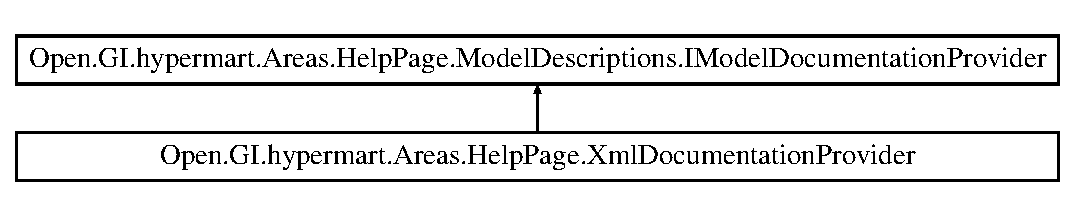
\includegraphics[height=2.000000cm]{interface_open_1_1_g_i_1_1hypermart_1_1_areas_1_1_help_page_1_1_model_descriptions_1_1_i_model_documentation_provider}
\end{center}
\end{figure}
\subsection*{Public Member Functions}
\begin{DoxyCompactItemize}
\item 
string \textbf{ Get\+Documentation} (Member\+Info member)
\begin{DoxyCompactList}\small\item\em Gets the documentation. \end{DoxyCompactList}\item 
string \textbf{ Get\+Documentation} (Type type)
\begin{DoxyCompactList}\small\item\em Gets the documentation. \end{DoxyCompactList}\end{DoxyCompactItemize}


\subsection{Detailed Description}




Definition at line 9 of file I\+Model\+Documentation\+Provider.\+cs.



\subsection{Member Function Documentation}
\mbox{\label{interface_open_1_1_g_i_1_1hypermart_1_1_areas_1_1_help_page_1_1_model_descriptions_1_1_i_model_documentation_provider_a27d4470da05e52051ae345515c17755a}} 
\index{Open\+::\+G\+I\+::hypermart\+::\+Areas\+::\+Help\+Page\+::\+Model\+Descriptions\+::\+I\+Model\+Documentation\+Provider@{Open\+::\+G\+I\+::hypermart\+::\+Areas\+::\+Help\+Page\+::\+Model\+Descriptions\+::\+I\+Model\+Documentation\+Provider}!Get\+Documentation@{Get\+Documentation}}
\index{Get\+Documentation@{Get\+Documentation}!Open\+::\+G\+I\+::hypermart\+::\+Areas\+::\+Help\+Page\+::\+Model\+Descriptions\+::\+I\+Model\+Documentation\+Provider@{Open\+::\+G\+I\+::hypermart\+::\+Areas\+::\+Help\+Page\+::\+Model\+Descriptions\+::\+I\+Model\+Documentation\+Provider}}
\subsubsection{Get\+Documentation()\hspace{0.1cm}{\footnotesize\ttfamily [1/2]}}
{\footnotesize\ttfamily string Open.\+G\+I.\+hypermart.\+Areas.\+Help\+Page.\+Model\+Descriptions.\+I\+Model\+Documentation\+Provider.\+Get\+Documentation (\begin{DoxyParamCaption}\item[{Member\+Info}]{member }\end{DoxyParamCaption})}



Gets the documentation. 


\begin{DoxyParams}{Parameters}
{\em member} & The member.\\
\hline
\end{DoxyParams}
\begin{DoxyReturn}{Returns}

\end{DoxyReturn}


Implemented in \textbf{ Open.\+G\+I.\+hypermart.\+Areas.\+Help\+Page.\+Xml\+Documentation\+Provider} \doxyref{}{p.}{class_open_1_1_g_i_1_1hypermart_1_1_areas_1_1_help_page_1_1_xml_documentation_provider_a1ba7e50dea71787a555f92306ec99efc}.

\mbox{\label{interface_open_1_1_g_i_1_1hypermart_1_1_areas_1_1_help_page_1_1_model_descriptions_1_1_i_model_documentation_provider_a047061b90c62930fc0a1dbcb09732bd3}} 
\index{Open\+::\+G\+I\+::hypermart\+::\+Areas\+::\+Help\+Page\+::\+Model\+Descriptions\+::\+I\+Model\+Documentation\+Provider@{Open\+::\+G\+I\+::hypermart\+::\+Areas\+::\+Help\+Page\+::\+Model\+Descriptions\+::\+I\+Model\+Documentation\+Provider}!Get\+Documentation@{Get\+Documentation}}
\index{Get\+Documentation@{Get\+Documentation}!Open\+::\+G\+I\+::hypermart\+::\+Areas\+::\+Help\+Page\+::\+Model\+Descriptions\+::\+I\+Model\+Documentation\+Provider@{Open\+::\+G\+I\+::hypermart\+::\+Areas\+::\+Help\+Page\+::\+Model\+Descriptions\+::\+I\+Model\+Documentation\+Provider}}
\subsubsection{Get\+Documentation()\hspace{0.1cm}{\footnotesize\ttfamily [2/2]}}
{\footnotesize\ttfamily string Open.\+G\+I.\+hypermart.\+Areas.\+Help\+Page.\+Model\+Descriptions.\+I\+Model\+Documentation\+Provider.\+Get\+Documentation (\begin{DoxyParamCaption}\item[{Type}]{type }\end{DoxyParamCaption})}



Gets the documentation. 


\begin{DoxyParams}{Parameters}
{\em type} & The type.\\
\hline
\end{DoxyParams}
\begin{DoxyReturn}{Returns}

\end{DoxyReturn}


Implemented in \textbf{ Open.\+G\+I.\+hypermart.\+Areas.\+Help\+Page.\+Xml\+Documentation\+Provider} \doxyref{}{p.}{class_open_1_1_g_i_1_1hypermart_1_1_areas_1_1_help_page_1_1_xml_documentation_provider_af096939cdb4e5a26bd20ae3341fad66c}.



The documentation for this interface was generated from the following file\+:\begin{DoxyCompactItemize}
\item 
C\+:/\+Projects/\+App-\/\+Utility-\/\+Store/\+Open.\+G\+I.\+hypermart/\+Areas/\+Help\+Page/\+Model\+Descriptions/\textbf{ I\+Model\+Documentation\+Provider.\+cs}\end{DoxyCompactItemize}

\hypertarget{class_open_1_1_g_i_1_1hypermart_1_1_areas_1_1_help_page_1_1_invalid_sample}{}\section{Open.\+G\+I.\+hypermart.\+Areas.\+Help\+Page.\+Invalid\+Sample Class Reference}
\label{class_open_1_1_g_i_1_1hypermart_1_1_areas_1_1_help_page_1_1_invalid_sample}\index{Open.\+G\+I.\+hypermart.\+Areas.\+Help\+Page.\+Invalid\+Sample@{Open.\+G\+I.\+hypermart.\+Areas.\+Help\+Page.\+Invalid\+Sample}}


This represents an invalid sample on the help page. There\textquotesingle{}s a display template named \hyperlink{class_open_1_1_g_i_1_1hypermart_1_1_areas_1_1_help_page_1_1_invalid_sample}{Invalid\+Sample} associated with this class.  


\subsection*{Public Member Functions}
\begin{DoxyCompactItemize}
\item 
\hyperlink{class_open_1_1_g_i_1_1hypermart_1_1_areas_1_1_help_page_1_1_invalid_sample_a27e0677e2227b94913ea3072e05094b1}{Invalid\+Sample} (string error\+Message)
\begin{DoxyCompactList}\small\item\em Initializes a new instance of the \hyperlink{class_open_1_1_g_i_1_1hypermart_1_1_areas_1_1_help_page_1_1_invalid_sample}{Invalid\+Sample} class. \end{DoxyCompactList}\item 
override bool \hyperlink{class_open_1_1_g_i_1_1hypermart_1_1_areas_1_1_help_page_1_1_invalid_sample_a3c5afe0e3460fccc63bb2b058cf13a8d}{Equals} (object obj)
\begin{DoxyCompactList}\small\item\em Determines whether the specified System.\+Object, is equal to this instance. \end{DoxyCompactList}\item 
override int \hyperlink{class_open_1_1_g_i_1_1hypermart_1_1_areas_1_1_help_page_1_1_invalid_sample_a804d4354478ebcdab08f85e34f138496}{Get\+Hash\+Code} ()
\begin{DoxyCompactList}\small\item\em Returns a hash code for this instance. \end{DoxyCompactList}\item 
override string \hyperlink{class_open_1_1_g_i_1_1hypermart_1_1_areas_1_1_help_page_1_1_invalid_sample_ac19ab8008f61f08252bad6d7c063e7bd}{To\+String} ()
\begin{DoxyCompactList}\small\item\em Returns a System.\+String that represents this instance. \end{DoxyCompactList}\end{DoxyCompactItemize}
\subsection*{Properties}
\begin{DoxyCompactItemize}
\item 
string \hyperlink{class_open_1_1_g_i_1_1hypermart_1_1_areas_1_1_help_page_1_1_invalid_sample_a89f95b69edc57c57963b214d0bc844af}{Error\+Message}\hspace{0.3cm}{\ttfamily  \mbox{[}get\mbox{]}}
\begin{DoxyCompactList}\small\item\em Gets the error message. \end{DoxyCompactList}\end{DoxyCompactItemize}


\subsection{Detailed Description}
This represents an invalid sample on the help page. There\textquotesingle{}s a display template named \hyperlink{class_open_1_1_g_i_1_1hypermart_1_1_areas_1_1_help_page_1_1_invalid_sample}{Invalid\+Sample} associated with this class. 



Definition at line 8 of file Invalid\+Sample.\+cs.



\subsection{Constructor \& Destructor Documentation}
\hypertarget{class_open_1_1_g_i_1_1hypermart_1_1_areas_1_1_help_page_1_1_invalid_sample_a27e0677e2227b94913ea3072e05094b1}{}\index{Open\+::\+G\+I\+::hypermart\+::\+Areas\+::\+Help\+Page\+::\+Invalid\+Sample@{Open\+::\+G\+I\+::hypermart\+::\+Areas\+::\+Help\+Page\+::\+Invalid\+Sample}!Invalid\+Sample@{Invalid\+Sample}}
\index{Invalid\+Sample@{Invalid\+Sample}!Open\+::\+G\+I\+::hypermart\+::\+Areas\+::\+Help\+Page\+::\+Invalid\+Sample@{Open\+::\+G\+I\+::hypermart\+::\+Areas\+::\+Help\+Page\+::\+Invalid\+Sample}}
\subsubsection[{Invalid\+Sample(string error\+Message)}]{\setlength{\rightskip}{0pt plus 5cm}Open.\+G\+I.\+hypermart.\+Areas.\+Help\+Page.\+Invalid\+Sample.\+Invalid\+Sample (
\begin{DoxyParamCaption}
\item[{string}]{error\+Message}
\end{DoxyParamCaption}
)}\label{class_open_1_1_g_i_1_1hypermart_1_1_areas_1_1_help_page_1_1_invalid_sample_a27e0677e2227b94913ea3072e05094b1}


Initializes a new instance of the \hyperlink{class_open_1_1_g_i_1_1hypermart_1_1_areas_1_1_help_page_1_1_invalid_sample}{Invalid\+Sample} class. 


\begin{DoxyParams}{Parameters}
{\em error\+Message} & The error message.\\
\hline
\end{DoxyParams}

\begin{DoxyExceptions}{Exceptions}
{\em System.\+Argument\+Null\+Exception} & error\+Message\\
\hline
\end{DoxyExceptions}


Definition at line 15 of file Invalid\+Sample.\+cs.



\subsection{Member Function Documentation}
\hypertarget{class_open_1_1_g_i_1_1hypermart_1_1_areas_1_1_help_page_1_1_invalid_sample_a3c5afe0e3460fccc63bb2b058cf13a8d}{}\index{Open\+::\+G\+I\+::hypermart\+::\+Areas\+::\+Help\+Page\+::\+Invalid\+Sample@{Open\+::\+G\+I\+::hypermart\+::\+Areas\+::\+Help\+Page\+::\+Invalid\+Sample}!Equals@{Equals}}
\index{Equals@{Equals}!Open\+::\+G\+I\+::hypermart\+::\+Areas\+::\+Help\+Page\+::\+Invalid\+Sample@{Open\+::\+G\+I\+::hypermart\+::\+Areas\+::\+Help\+Page\+::\+Invalid\+Sample}}
\subsubsection[{Equals(object obj)}]{\setlength{\rightskip}{0pt plus 5cm}override bool Open.\+G\+I.\+hypermart.\+Areas.\+Help\+Page.\+Invalid\+Sample.\+Equals (
\begin{DoxyParamCaption}
\item[{object}]{obj}
\end{DoxyParamCaption}
)}\label{class_open_1_1_g_i_1_1hypermart_1_1_areas_1_1_help_page_1_1_invalid_sample_a3c5afe0e3460fccc63bb2b058cf13a8d}


Determines whether the specified System.\+Object, is equal to this instance. 


\begin{DoxyParams}{Parameters}
{\em obj} & The System.\+Object to compare with this instance.\\
\hline
\end{DoxyParams}
\begin{DoxyReturn}{Returns}
{\ttfamily true} if the specified System.\+Object is equal to this instance; otherwise, {\ttfamily false}. 
\end{DoxyReturn}


Definition at line 39 of file Invalid\+Sample.\+cs.

\hypertarget{class_open_1_1_g_i_1_1hypermart_1_1_areas_1_1_help_page_1_1_invalid_sample_a804d4354478ebcdab08f85e34f138496}{}\index{Open\+::\+G\+I\+::hypermart\+::\+Areas\+::\+Help\+Page\+::\+Invalid\+Sample@{Open\+::\+G\+I\+::hypermart\+::\+Areas\+::\+Help\+Page\+::\+Invalid\+Sample}!Get\+Hash\+Code@{Get\+Hash\+Code}}
\index{Get\+Hash\+Code@{Get\+Hash\+Code}!Open\+::\+G\+I\+::hypermart\+::\+Areas\+::\+Help\+Page\+::\+Invalid\+Sample@{Open\+::\+G\+I\+::hypermart\+::\+Areas\+::\+Help\+Page\+::\+Invalid\+Sample}}
\subsubsection[{Get\+Hash\+Code()}]{\setlength{\rightskip}{0pt plus 5cm}override int Open.\+G\+I.\+hypermart.\+Areas.\+Help\+Page.\+Invalid\+Sample.\+Get\+Hash\+Code (
\begin{DoxyParamCaption}
{}
\end{DoxyParamCaption}
)}\label{class_open_1_1_g_i_1_1hypermart_1_1_areas_1_1_help_page_1_1_invalid_sample_a804d4354478ebcdab08f85e34f138496}


Returns a hash code for this instance. 

\begin{DoxyReturn}{Returns}
A hash code for this instance, suitable for use in hashing algorithms and data structures like a hash table. 
\end{DoxyReturn}


Definition at line 51 of file Invalid\+Sample.\+cs.

\hypertarget{class_open_1_1_g_i_1_1hypermart_1_1_areas_1_1_help_page_1_1_invalid_sample_ac19ab8008f61f08252bad6d7c063e7bd}{}\index{Open\+::\+G\+I\+::hypermart\+::\+Areas\+::\+Help\+Page\+::\+Invalid\+Sample@{Open\+::\+G\+I\+::hypermart\+::\+Areas\+::\+Help\+Page\+::\+Invalid\+Sample}!To\+String@{To\+String}}
\index{To\+String@{To\+String}!Open\+::\+G\+I\+::hypermart\+::\+Areas\+::\+Help\+Page\+::\+Invalid\+Sample@{Open\+::\+G\+I\+::hypermart\+::\+Areas\+::\+Help\+Page\+::\+Invalid\+Sample}}
\subsubsection[{To\+String()}]{\setlength{\rightskip}{0pt plus 5cm}override string Open.\+G\+I.\+hypermart.\+Areas.\+Help\+Page.\+Invalid\+Sample.\+To\+String (
\begin{DoxyParamCaption}
{}
\end{DoxyParamCaption}
)}\label{class_open_1_1_g_i_1_1hypermart_1_1_areas_1_1_help_page_1_1_invalid_sample_ac19ab8008f61f08252bad6d7c063e7bd}


Returns a System.\+String that represents this instance. 

\begin{DoxyReturn}{Returns}
A System.\+String that represents this instance. 
\end{DoxyReturn}


Definition at line 62 of file Invalid\+Sample.\+cs.



\subsection{Property Documentation}
\hypertarget{class_open_1_1_g_i_1_1hypermart_1_1_areas_1_1_help_page_1_1_invalid_sample_a89f95b69edc57c57963b214d0bc844af}{}\index{Open\+::\+G\+I\+::hypermart\+::\+Areas\+::\+Help\+Page\+::\+Invalid\+Sample@{Open\+::\+G\+I\+::hypermart\+::\+Areas\+::\+Help\+Page\+::\+Invalid\+Sample}!Error\+Message@{Error\+Message}}
\index{Error\+Message@{Error\+Message}!Open\+::\+G\+I\+::hypermart\+::\+Areas\+::\+Help\+Page\+::\+Invalid\+Sample@{Open\+::\+G\+I\+::hypermart\+::\+Areas\+::\+Help\+Page\+::\+Invalid\+Sample}}
\subsubsection[{Error\+Message}]{\setlength{\rightskip}{0pt plus 5cm}string Open.\+G\+I.\+hypermart.\+Areas.\+Help\+Page.\+Invalid\+Sample.\+Error\+Message\hspace{0.3cm}{\ttfamily [get]}}\label{class_open_1_1_g_i_1_1hypermart_1_1_areas_1_1_help_page_1_1_invalid_sample_a89f95b69edc57c57963b214d0bc844af}


Gets the error message. 

The error message. 

Definition at line 30 of file Invalid\+Sample.\+cs.



The documentation for this class was generated from the following file\+:\begin{DoxyCompactItemize}
\item 
C\+:/\+Projects/\+App-\/\+Utility-\/\+Store/\+Open.\+G\+I.\+hypermart/\+Areas/\+Help\+Page/\+Sample\+Generation/\hyperlink{_invalid_sample_8cs}{Invalid\+Sample.\+cs}\end{DoxyCompactItemize}

\hypertarget{class_open_1_1_g_i_1_1hypermart_1_1_areas_1_1_help_page_1_1_model_descriptions_1_1_key_value_pair_model_description}{}\section{Open.\+G\+I.\+hypermart.\+Areas.\+Help\+Page.\+Model\+Descriptions.\+Key\+Value\+Pair\+Model\+Description Class Reference}
\label{class_open_1_1_g_i_1_1hypermart_1_1_areas_1_1_help_page_1_1_model_descriptions_1_1_key_value_pair_model_description}\index{Open.\+G\+I.\+hypermart.\+Areas.\+Help\+Page.\+Model\+Descriptions.\+Key\+Value\+Pair\+Model\+Description@{Open.\+G\+I.\+hypermart.\+Areas.\+Help\+Page.\+Model\+Descriptions.\+Key\+Value\+Pair\+Model\+Description}}


 


Inheritance diagram for Open.\+G\+I.\+hypermart.\+Areas.\+Help\+Page.\+Model\+Descriptions.\+Key\+Value\+Pair\+Model\+Description\+:\begin{figure}[H]
\begin{center}
\leavevmode
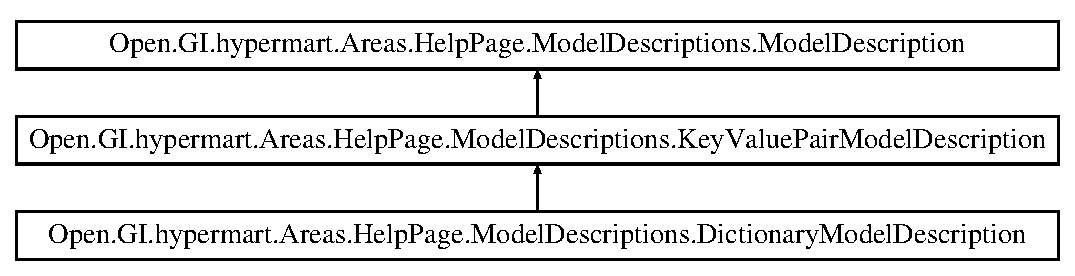
\includegraphics[height=3.000000cm]{class_open_1_1_g_i_1_1hypermart_1_1_areas_1_1_help_page_1_1_model_descriptions_1_1_key_value_pair_model_description}
\end{center}
\end{figure}
\subsection*{Properties}
\begin{DoxyCompactItemize}
\item 
\hyperlink{class_open_1_1_g_i_1_1hypermart_1_1_areas_1_1_help_page_1_1_model_descriptions_1_1_model_description}{Model\+Description} \hyperlink{class_open_1_1_g_i_1_1hypermart_1_1_areas_1_1_help_page_1_1_model_descriptions_1_1_key_value_pair_model_description_a76ccd9d3ad532ce5a56b52d15d84c324}{Key\+Model\+Description}\hspace{0.3cm}{\ttfamily  \mbox{[}get, set\mbox{]}}
\begin{DoxyCompactList}\small\item\em Gets or sets the key model description. \end{DoxyCompactList}\item 
\hyperlink{class_open_1_1_g_i_1_1hypermart_1_1_areas_1_1_help_page_1_1_model_descriptions_1_1_model_description}{Model\+Description} \hyperlink{class_open_1_1_g_i_1_1hypermart_1_1_areas_1_1_help_page_1_1_model_descriptions_1_1_key_value_pair_model_description_a5bcf18b1e78df6ba8b0cbc001a11ace6}{Value\+Model\+Description}\hspace{0.3cm}{\ttfamily  \mbox{[}get, set\mbox{]}}
\begin{DoxyCompactList}\small\item\em Gets or sets the value model description. \end{DoxyCompactList}\end{DoxyCompactItemize}


\subsection{Detailed Description}


\begin{DoxySeeAlso}{See also}
\hyperlink{class_open_1_1_g_i_1_1hypermart_1_1_areas_1_1_help_page_1_1_model_descriptions_1_1_model_description}{Open.\+G\+I.\+hypermart.\+Areas.\+Help\+Page.\+Model\+Descriptions.\+Model\+Description}


\end{DoxySeeAlso}


\subsection{Property Documentation}
\hypertarget{class_open_1_1_g_i_1_1hypermart_1_1_areas_1_1_help_page_1_1_model_descriptions_1_1_key_value_pair_model_description_a76ccd9d3ad532ce5a56b52d15d84c324}{}\label{class_open_1_1_g_i_1_1hypermart_1_1_areas_1_1_help_page_1_1_model_descriptions_1_1_key_value_pair_model_description_a76ccd9d3ad532ce5a56b52d15d84c324} 
\index{Open\+::\+G\+I\+::hypermart\+::\+Areas\+::\+Help\+Page\+::\+Model\+Descriptions\+::\+Key\+Value\+Pair\+Model\+Description@{Open\+::\+G\+I\+::hypermart\+::\+Areas\+::\+Help\+Page\+::\+Model\+Descriptions\+::\+Key\+Value\+Pair\+Model\+Description}!Key\+Model\+Description@{Key\+Model\+Description}}
\index{Key\+Model\+Description@{Key\+Model\+Description}!Open\+::\+G\+I\+::hypermart\+::\+Areas\+::\+Help\+Page\+::\+Model\+Descriptions\+::\+Key\+Value\+Pair\+Model\+Description@{Open\+::\+G\+I\+::hypermart\+::\+Areas\+::\+Help\+Page\+::\+Model\+Descriptions\+::\+Key\+Value\+Pair\+Model\+Description}}
\subsubsection{\texorpdfstring{Key\+Model\+Description}{KeyModelDescription}}
{\footnotesize\ttfamily \hyperlink{class_open_1_1_g_i_1_1hypermart_1_1_areas_1_1_help_page_1_1_model_descriptions_1_1_model_description}{Model\+Description} Open.\+G\+I.\+hypermart.\+Areas.\+Help\+Page.\+Model\+Descriptions.\+Key\+Value\+Pair\+Model\+Description.\+Key\+Model\+Description\hspace{0.3cm}{\ttfamily [get]}, {\ttfamily [set]}}



Gets or sets the key model description. 

The key model description. \hypertarget{class_open_1_1_g_i_1_1hypermart_1_1_areas_1_1_help_page_1_1_model_descriptions_1_1_key_value_pair_model_description_a5bcf18b1e78df6ba8b0cbc001a11ace6}{}\label{class_open_1_1_g_i_1_1hypermart_1_1_areas_1_1_help_page_1_1_model_descriptions_1_1_key_value_pair_model_description_a5bcf18b1e78df6ba8b0cbc001a11ace6} 
\index{Open\+::\+G\+I\+::hypermart\+::\+Areas\+::\+Help\+Page\+::\+Model\+Descriptions\+::\+Key\+Value\+Pair\+Model\+Description@{Open\+::\+G\+I\+::hypermart\+::\+Areas\+::\+Help\+Page\+::\+Model\+Descriptions\+::\+Key\+Value\+Pair\+Model\+Description}!Value\+Model\+Description@{Value\+Model\+Description}}
\index{Value\+Model\+Description@{Value\+Model\+Description}!Open\+::\+G\+I\+::hypermart\+::\+Areas\+::\+Help\+Page\+::\+Model\+Descriptions\+::\+Key\+Value\+Pair\+Model\+Description@{Open\+::\+G\+I\+::hypermart\+::\+Areas\+::\+Help\+Page\+::\+Model\+Descriptions\+::\+Key\+Value\+Pair\+Model\+Description}}
\subsubsection{\texorpdfstring{Value\+Model\+Description}{ValueModelDescription}}
{\footnotesize\ttfamily \hyperlink{class_open_1_1_g_i_1_1hypermart_1_1_areas_1_1_help_page_1_1_model_descriptions_1_1_model_description}{Model\+Description} Open.\+G\+I.\+hypermart.\+Areas.\+Help\+Page.\+Model\+Descriptions.\+Key\+Value\+Pair\+Model\+Description.\+Value\+Model\+Description\hspace{0.3cm}{\ttfamily [get]}, {\ttfamily [set]}}



Gets or sets the value model description. 

The value model description. 

The documentation for this class was generated from the following file\+:\begin{DoxyCompactItemize}
\item 
C\+:/\+Projects/\+App-\/\+Utility-\/\+Store/\+Open.\+G\+I.\+hypermart/\+Areas/\+Help\+Page/\+Model\+Descriptions/\hyperlink{_key_value_pair_model_description_8cs}{Key\+Value\+Pair\+Model\+Description.\+cs}\end{DoxyCompactItemize}

\hypertarget{class_open_1_1_g_i_1_1hypermart_1_1_models_1_1_model1_container}{}\section{Open.\+G\+I.\+hypermart.\+Models.\+Model1\+Container Class Reference}
\label{class_open_1_1_g_i_1_1hypermart_1_1_models_1_1_model1_container}\index{Open.\+G\+I.\+hypermart.\+Models.\+Model1\+Container@{Open.\+G\+I.\+hypermart.\+Models.\+Model1\+Container}}
Inheritance diagram for Open.\+G\+I.\+hypermart.\+Models.\+Model1\+Container\+:\begin{figure}[H]
\begin{center}
\leavevmode
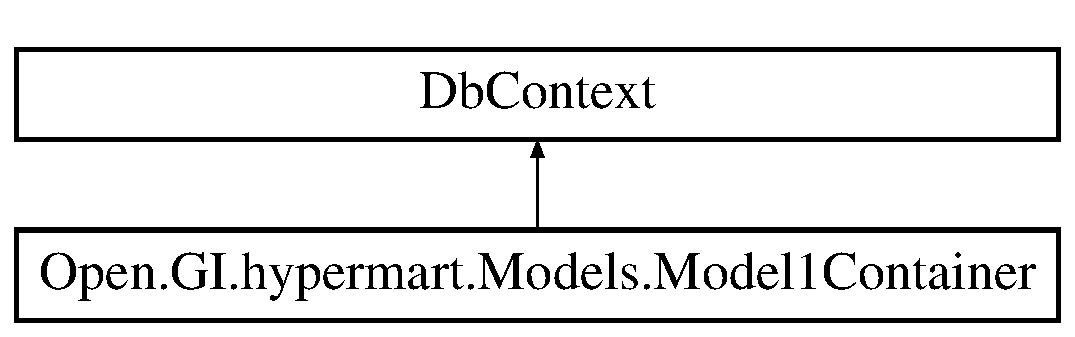
\includegraphics[height=2.000000cm]{class_open_1_1_g_i_1_1hypermart_1_1_models_1_1_model1_container}
\end{center}
\end{figure}
\subsection*{Public Member Functions}
\begin{DoxyCompactItemize}
\item 
\hyperlink{class_open_1_1_g_i_1_1hypermart_1_1_models_1_1_model1_container_a8d957335d29c47427c9d9062c11e6205}{Model1\+Container} ()
\end{DoxyCompactItemize}
\subsection*{Protected Member Functions}
\begin{DoxyCompactItemize}
\item 
override void \hyperlink{class_open_1_1_g_i_1_1hypermart_1_1_models_1_1_model1_container_a738eaf983c5fc89665bff3d90f9fb188}{On\+Model\+Creating} (Db\+Model\+Builder model\+Builder)
\end{DoxyCompactItemize}
\subsection*{Properties}
\begin{DoxyCompactItemize}
\item 
virtual Db\+Set$<$ \hyperlink{class_open_1_1_g_i_1_1hypermart_1_1_models_1_1_file}{File} $>$ \hyperlink{class_open_1_1_g_i_1_1hypermart_1_1_models_1_1_model1_container_a446f391e8b281cf4e3e71f369940189c}{Files}\hspace{0.3cm}{\ttfamily  \mbox{[}get, set\mbox{]}}
\item 
virtual Db\+Set$<$ \hyperlink{class_open_1_1_g_i_1_1hypermart_1_1_models_1_1_file_platform}{File\+Platform} $>$ \hyperlink{class_open_1_1_g_i_1_1hypermart_1_1_models_1_1_model1_container_ad8999f3ba131f3c46c9162b2eff4c7f9}{File\+Platforms}\hspace{0.3cm}{\ttfamily  \mbox{[}get, set\mbox{]}}
\item 
virtual Db\+Set$<$ \hyperlink{class_open_1_1_g_i_1_1hypermart_1_1_models_1_1_platform}{Platform} $>$ \hyperlink{class_open_1_1_g_i_1_1hypermart_1_1_models_1_1_model1_container_a47b249679414da9e63797516568ddb73}{Platforms}\hspace{0.3cm}{\ttfamily  \mbox{[}get, set\mbox{]}}
\item 
virtual Db\+Set$<$ \hyperlink{class_open_1_1_g_i_1_1hypermart_1_1_models_1_1_product}{Product} $>$ \hyperlink{class_open_1_1_g_i_1_1hypermart_1_1_models_1_1_model1_container_a3152c9cb162bad57e707fb1a6b48152c}{Products}\hspace{0.3cm}{\ttfamily  \mbox{[}get, set\mbox{]}}
\item 
virtual Db\+Set$<$ \hyperlink{class_open_1_1_g_i_1_1hypermart_1_1_models_1_1_screenshot}{Screenshot} $>$ \hyperlink{class_open_1_1_g_i_1_1hypermart_1_1_models_1_1_model1_container_a16840948ed271ebac66728f3398b6696}{Screenshots}\hspace{0.3cm}{\ttfamily  \mbox{[}get, set\mbox{]}}
\end{DoxyCompactItemize}


\subsection{Detailed Description}


Definition at line 16 of file Model1.\+Context.\+cs.



\subsection{Constructor \& Destructor Documentation}
\hypertarget{class_open_1_1_g_i_1_1hypermart_1_1_models_1_1_model1_container_a8d957335d29c47427c9d9062c11e6205}{}\index{Open\+::\+G\+I\+::hypermart\+::\+Models\+::\+Model1\+Container@{Open\+::\+G\+I\+::hypermart\+::\+Models\+::\+Model1\+Container}!Model1\+Container@{Model1\+Container}}
\index{Model1\+Container@{Model1\+Container}!Open\+::\+G\+I\+::hypermart\+::\+Models\+::\+Model1\+Container@{Open\+::\+G\+I\+::hypermart\+::\+Models\+::\+Model1\+Container}}
\subsubsection[{Model1\+Container()}]{\setlength{\rightskip}{0pt plus 5cm}Open.\+G\+I.\+hypermart.\+Models.\+Model1\+Container.\+Model1\+Container (
\begin{DoxyParamCaption}
{}
\end{DoxyParamCaption}
)}\label{class_open_1_1_g_i_1_1hypermart_1_1_models_1_1_model1_container_a8d957335d29c47427c9d9062c11e6205}


Definition at line 18 of file Model1.\+Context.\+cs.



\subsection{Member Function Documentation}
\hypertarget{class_open_1_1_g_i_1_1hypermart_1_1_models_1_1_model1_container_a738eaf983c5fc89665bff3d90f9fb188}{}\index{Open\+::\+G\+I\+::hypermart\+::\+Models\+::\+Model1\+Container@{Open\+::\+G\+I\+::hypermart\+::\+Models\+::\+Model1\+Container}!On\+Model\+Creating@{On\+Model\+Creating}}
\index{On\+Model\+Creating@{On\+Model\+Creating}!Open\+::\+G\+I\+::hypermart\+::\+Models\+::\+Model1\+Container@{Open\+::\+G\+I\+::hypermart\+::\+Models\+::\+Model1\+Container}}
\subsubsection[{On\+Model\+Creating(\+Db\+Model\+Builder model\+Builder)}]{\setlength{\rightskip}{0pt plus 5cm}override void Open.\+G\+I.\+hypermart.\+Models.\+Model1\+Container.\+On\+Model\+Creating (
\begin{DoxyParamCaption}
\item[{Db\+Model\+Builder}]{model\+Builder}
\end{DoxyParamCaption}
)\hspace{0.3cm}{\ttfamily [protected]}}\label{class_open_1_1_g_i_1_1hypermart_1_1_models_1_1_model1_container_a738eaf983c5fc89665bff3d90f9fb188}


Definition at line 23 of file Model1.\+Context.\+cs.



\subsection{Property Documentation}
\hypertarget{class_open_1_1_g_i_1_1hypermart_1_1_models_1_1_model1_container_ad8999f3ba131f3c46c9162b2eff4c7f9}{}\index{Open\+::\+G\+I\+::hypermart\+::\+Models\+::\+Model1\+Container@{Open\+::\+G\+I\+::hypermart\+::\+Models\+::\+Model1\+Container}!File\+Platforms@{File\+Platforms}}
\index{File\+Platforms@{File\+Platforms}!Open\+::\+G\+I\+::hypermart\+::\+Models\+::\+Model1\+Container@{Open\+::\+G\+I\+::hypermart\+::\+Models\+::\+Model1\+Container}}
\subsubsection[{File\+Platforms}]{\setlength{\rightskip}{0pt plus 5cm}virtual Db\+Set$<${\bf File\+Platform}$>$ Open.\+G\+I.\+hypermart.\+Models.\+Model1\+Container.\+File\+Platforms\hspace{0.3cm}{\ttfamily [get]}, {\ttfamily [set]}}\label{class_open_1_1_g_i_1_1hypermart_1_1_models_1_1_model1_container_ad8999f3ba131f3c46c9162b2eff4c7f9}


Definition at line 29 of file Model1.\+Context.\+cs.

\hypertarget{class_open_1_1_g_i_1_1hypermart_1_1_models_1_1_model1_container_a446f391e8b281cf4e3e71f369940189c}{}\index{Open\+::\+G\+I\+::hypermart\+::\+Models\+::\+Model1\+Container@{Open\+::\+G\+I\+::hypermart\+::\+Models\+::\+Model1\+Container}!Files@{Files}}
\index{Files@{Files}!Open\+::\+G\+I\+::hypermart\+::\+Models\+::\+Model1\+Container@{Open\+::\+G\+I\+::hypermart\+::\+Models\+::\+Model1\+Container}}
\subsubsection[{Files}]{\setlength{\rightskip}{0pt plus 5cm}virtual Db\+Set$<${\bf File}$>$ Open.\+G\+I.\+hypermart.\+Models.\+Model1\+Container.\+Files\hspace{0.3cm}{\ttfamily [get]}, {\ttfamily [set]}}\label{class_open_1_1_g_i_1_1hypermart_1_1_models_1_1_model1_container_a446f391e8b281cf4e3e71f369940189c}


Definition at line 28 of file Model1.\+Context.\+cs.

\hypertarget{class_open_1_1_g_i_1_1hypermart_1_1_models_1_1_model1_container_a47b249679414da9e63797516568ddb73}{}\index{Open\+::\+G\+I\+::hypermart\+::\+Models\+::\+Model1\+Container@{Open\+::\+G\+I\+::hypermart\+::\+Models\+::\+Model1\+Container}!Platforms@{Platforms}}
\index{Platforms@{Platforms}!Open\+::\+G\+I\+::hypermart\+::\+Models\+::\+Model1\+Container@{Open\+::\+G\+I\+::hypermart\+::\+Models\+::\+Model1\+Container}}
\subsubsection[{Platforms}]{\setlength{\rightskip}{0pt plus 5cm}virtual Db\+Set$<${\bf Platform}$>$ Open.\+G\+I.\+hypermart.\+Models.\+Model1\+Container.\+Platforms\hspace{0.3cm}{\ttfamily [get]}, {\ttfamily [set]}}\label{class_open_1_1_g_i_1_1hypermart_1_1_models_1_1_model1_container_a47b249679414da9e63797516568ddb73}


Definition at line 30 of file Model1.\+Context.\+cs.

\hypertarget{class_open_1_1_g_i_1_1hypermart_1_1_models_1_1_model1_container_a3152c9cb162bad57e707fb1a6b48152c}{}\index{Open\+::\+G\+I\+::hypermart\+::\+Models\+::\+Model1\+Container@{Open\+::\+G\+I\+::hypermart\+::\+Models\+::\+Model1\+Container}!Products@{Products}}
\index{Products@{Products}!Open\+::\+G\+I\+::hypermart\+::\+Models\+::\+Model1\+Container@{Open\+::\+G\+I\+::hypermart\+::\+Models\+::\+Model1\+Container}}
\subsubsection[{Products}]{\setlength{\rightskip}{0pt plus 5cm}virtual Db\+Set$<${\bf Product}$>$ Open.\+G\+I.\+hypermart.\+Models.\+Model1\+Container.\+Products\hspace{0.3cm}{\ttfamily [get]}, {\ttfamily [set]}}\label{class_open_1_1_g_i_1_1hypermart_1_1_models_1_1_model1_container_a3152c9cb162bad57e707fb1a6b48152c}


Definition at line 31 of file Model1.\+Context.\+cs.

\hypertarget{class_open_1_1_g_i_1_1hypermart_1_1_models_1_1_model1_container_a16840948ed271ebac66728f3398b6696}{}\index{Open\+::\+G\+I\+::hypermart\+::\+Models\+::\+Model1\+Container@{Open\+::\+G\+I\+::hypermart\+::\+Models\+::\+Model1\+Container}!Screenshots@{Screenshots}}
\index{Screenshots@{Screenshots}!Open\+::\+G\+I\+::hypermart\+::\+Models\+::\+Model1\+Container@{Open\+::\+G\+I\+::hypermart\+::\+Models\+::\+Model1\+Container}}
\subsubsection[{Screenshots}]{\setlength{\rightskip}{0pt plus 5cm}virtual Db\+Set$<${\bf Screenshot}$>$ Open.\+G\+I.\+hypermart.\+Models.\+Model1\+Container.\+Screenshots\hspace{0.3cm}{\ttfamily [get]}, {\ttfamily [set]}}\label{class_open_1_1_g_i_1_1hypermart_1_1_models_1_1_model1_container_a16840948ed271ebac66728f3398b6696}


Definition at line 32 of file Model1.\+Context.\+cs.



The documentation for this class was generated from the following file\+:\begin{DoxyCompactItemize}
\item 
C\+:/\+Projects/\+App-\/\+Utility-\/\+Store/\+Open.\+G\+I.\+hypermart/\+W\+I\+P/\hyperlink{_model1_8_context_8cs}{Model1.\+Context.\+cs}\end{DoxyCompactItemize}

\hypertarget{class_open_1_1_g_i_1_1hypermart_1_1_areas_1_1_help_page_1_1_model_descriptions_1_1_model_description}{}\section{Open.\+G\+I.\+hypermart.\+Areas.\+Help\+Page.\+Model\+Descriptions.\+Model\+Description Class Reference}
\label{class_open_1_1_g_i_1_1hypermart_1_1_areas_1_1_help_page_1_1_model_descriptions_1_1_model_description}\index{Open.\+G\+I.\+hypermart.\+Areas.\+Help\+Page.\+Model\+Descriptions.\+Model\+Description@{Open.\+G\+I.\+hypermart.\+Areas.\+Help\+Page.\+Model\+Descriptions.\+Model\+Description}}


Describes a type model.  


Inheritance diagram for Open.\+G\+I.\+hypermart.\+Areas.\+Help\+Page.\+Model\+Descriptions.\+Model\+Description\+:\begin{figure}[H]
\begin{center}
\leavevmode
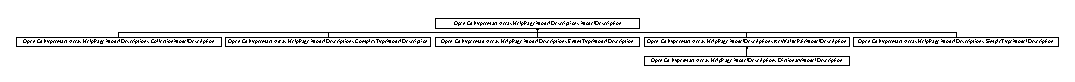
\includegraphics[height=0.652427cm]{class_open_1_1_g_i_1_1hypermart_1_1_areas_1_1_help_page_1_1_model_descriptions_1_1_model_description}
\end{center}
\end{figure}
\subsection*{Properties}
\begin{DoxyCompactItemize}
\item 
string \hyperlink{class_open_1_1_g_i_1_1hypermart_1_1_areas_1_1_help_page_1_1_model_descriptions_1_1_model_description_af08e1f5a6e3a28669b602926cb9a07b9}{Documentation}\hspace{0.3cm}{\ttfamily  \mbox{[}get, set\mbox{]}}
\begin{DoxyCompactList}\small\item\em Gets or sets the documentation. \end{DoxyCompactList}\item 
Type \hyperlink{class_open_1_1_g_i_1_1hypermart_1_1_areas_1_1_help_page_1_1_model_descriptions_1_1_model_description_ab41d4f322450e3a2cde611673ca4abb1}{Model\+Type}\hspace{0.3cm}{\ttfamily  \mbox{[}get, set\mbox{]}}
\begin{DoxyCompactList}\small\item\em Gets or sets the type of the model. \end{DoxyCompactList}\item 
string \hyperlink{class_open_1_1_g_i_1_1hypermart_1_1_areas_1_1_help_page_1_1_model_descriptions_1_1_model_description_aa5a42ec74b1d880ce15fd12b8ef0baf9}{Name}\hspace{0.3cm}{\ttfamily  \mbox{[}get, set\mbox{]}}
\begin{DoxyCompactList}\small\item\em Gets or sets the name. \end{DoxyCompactList}\end{DoxyCompactItemize}


\subsection{Detailed Description}
Describes a type model. 



\subsection{Property Documentation}
\hypertarget{class_open_1_1_g_i_1_1hypermart_1_1_areas_1_1_help_page_1_1_model_descriptions_1_1_model_description_af08e1f5a6e3a28669b602926cb9a07b9}{}\label{class_open_1_1_g_i_1_1hypermart_1_1_areas_1_1_help_page_1_1_model_descriptions_1_1_model_description_af08e1f5a6e3a28669b602926cb9a07b9} 
\index{Open\+::\+G\+I\+::hypermart\+::\+Areas\+::\+Help\+Page\+::\+Model\+Descriptions\+::\+Model\+Description@{Open\+::\+G\+I\+::hypermart\+::\+Areas\+::\+Help\+Page\+::\+Model\+Descriptions\+::\+Model\+Description}!Documentation@{Documentation}}
\index{Documentation@{Documentation}!Open\+::\+G\+I\+::hypermart\+::\+Areas\+::\+Help\+Page\+::\+Model\+Descriptions\+::\+Model\+Description@{Open\+::\+G\+I\+::hypermart\+::\+Areas\+::\+Help\+Page\+::\+Model\+Descriptions\+::\+Model\+Description}}
\subsubsection{\texorpdfstring{Documentation}{Documentation}}
{\footnotesize\ttfamily string Open.\+G\+I.\+hypermart.\+Areas.\+Help\+Page.\+Model\+Descriptions.\+Model\+Description.\+Documentation\hspace{0.3cm}{\ttfamily [get]}, {\ttfamily [set]}}



Gets or sets the documentation. 

The documentation. \hypertarget{class_open_1_1_g_i_1_1hypermart_1_1_areas_1_1_help_page_1_1_model_descriptions_1_1_model_description_ab41d4f322450e3a2cde611673ca4abb1}{}\label{class_open_1_1_g_i_1_1hypermart_1_1_areas_1_1_help_page_1_1_model_descriptions_1_1_model_description_ab41d4f322450e3a2cde611673ca4abb1} 
\index{Open\+::\+G\+I\+::hypermart\+::\+Areas\+::\+Help\+Page\+::\+Model\+Descriptions\+::\+Model\+Description@{Open\+::\+G\+I\+::hypermart\+::\+Areas\+::\+Help\+Page\+::\+Model\+Descriptions\+::\+Model\+Description}!Model\+Type@{Model\+Type}}
\index{Model\+Type@{Model\+Type}!Open\+::\+G\+I\+::hypermart\+::\+Areas\+::\+Help\+Page\+::\+Model\+Descriptions\+::\+Model\+Description@{Open\+::\+G\+I\+::hypermart\+::\+Areas\+::\+Help\+Page\+::\+Model\+Descriptions\+::\+Model\+Description}}
\subsubsection{\texorpdfstring{Model\+Type}{ModelType}}
{\footnotesize\ttfamily Type Open.\+G\+I.\+hypermart.\+Areas.\+Help\+Page.\+Model\+Descriptions.\+Model\+Description.\+Model\+Type\hspace{0.3cm}{\ttfamily [get]}, {\ttfamily [set]}}



Gets or sets the type of the model. 

The type of the model. \hypertarget{class_open_1_1_g_i_1_1hypermart_1_1_areas_1_1_help_page_1_1_model_descriptions_1_1_model_description_aa5a42ec74b1d880ce15fd12b8ef0baf9}{}\label{class_open_1_1_g_i_1_1hypermart_1_1_areas_1_1_help_page_1_1_model_descriptions_1_1_model_description_aa5a42ec74b1d880ce15fd12b8ef0baf9} 
\index{Open\+::\+G\+I\+::hypermart\+::\+Areas\+::\+Help\+Page\+::\+Model\+Descriptions\+::\+Model\+Description@{Open\+::\+G\+I\+::hypermart\+::\+Areas\+::\+Help\+Page\+::\+Model\+Descriptions\+::\+Model\+Description}!Name@{Name}}
\index{Name@{Name}!Open\+::\+G\+I\+::hypermart\+::\+Areas\+::\+Help\+Page\+::\+Model\+Descriptions\+::\+Model\+Description@{Open\+::\+G\+I\+::hypermart\+::\+Areas\+::\+Help\+Page\+::\+Model\+Descriptions\+::\+Model\+Description}}
\subsubsection{\texorpdfstring{Name}{Name}}
{\footnotesize\ttfamily string Open.\+G\+I.\+hypermart.\+Areas.\+Help\+Page.\+Model\+Descriptions.\+Model\+Description.\+Name\hspace{0.3cm}{\ttfamily [get]}, {\ttfamily [set]}}



Gets or sets the name. 

The name. 

The documentation for this class was generated from the following file\+:\begin{DoxyCompactItemize}
\item 
C\+:/\+Projects/\+App-\/\+Utility-\/\+Store/\+Open.\+G\+I.\+hypermart/\+Areas/\+Help\+Page/\+Model\+Descriptions/\hyperlink{_model_description_8cs}{Model\+Description.\+cs}\end{DoxyCompactItemize}

\hypertarget{class_open_1_1_g_i_1_1hypermart_1_1_areas_1_1_help_page_1_1_model_descriptions_1_1_model_description_generator}{}\section{Open.\+G\+I.\+hypermart.\+Areas.\+Help\+Page.\+Model\+Descriptions.\+Model\+Description\+Generator Class Reference}
\label{class_open_1_1_g_i_1_1hypermart_1_1_areas_1_1_help_page_1_1_model_descriptions_1_1_model_description_generator}\index{Open.\+G\+I.\+hypermart.\+Areas.\+Help\+Page.\+Model\+Descriptions.\+Model\+Description\+Generator@{Open.\+G\+I.\+hypermart.\+Areas.\+Help\+Page.\+Model\+Descriptions.\+Model\+Description\+Generator}}


Generates model descriptions for given types.  


\subsection*{Public Member Functions}
\begin{DoxyCompactItemize}
\item 
\hyperlink{class_open_1_1_g_i_1_1hypermart_1_1_areas_1_1_help_page_1_1_model_descriptions_1_1_model_description_generator_a56c6ca4b29667cf648929f4bbedca964}{Model\+Description\+Generator} (Http\+Configuration config)
\begin{DoxyCompactList}\small\item\em Initializes a new instance of the \hyperlink{class_open_1_1_g_i_1_1hypermart_1_1_areas_1_1_help_page_1_1_model_descriptions_1_1_model_description_generator}{Model\+Description\+Generator} class. \end{DoxyCompactList}\item 
\hyperlink{class_open_1_1_g_i_1_1hypermart_1_1_areas_1_1_help_page_1_1_model_descriptions_1_1_model_description}{Model\+Description} \hyperlink{class_open_1_1_g_i_1_1hypermart_1_1_areas_1_1_help_page_1_1_model_descriptions_1_1_model_description_generator_aa693e668d64aa73688aaa4fc080eb525}{Get\+Or\+Create\+Model\+Description} (Type model\+Type)
\begin{DoxyCompactList}\small\item\em Gets the or create model description. \end{DoxyCompactList}\end{DoxyCompactItemize}
\subsection*{Properties}
\begin{DoxyCompactItemize}
\item 
Dictionary$<$ string, \hyperlink{class_open_1_1_g_i_1_1hypermart_1_1_areas_1_1_help_page_1_1_model_descriptions_1_1_model_description}{Model\+Description} $>$ \hyperlink{class_open_1_1_g_i_1_1hypermart_1_1_areas_1_1_help_page_1_1_model_descriptions_1_1_model_description_generator_ad4d703c3da52e11a1e52c12ae04e88a6}{Generated\+Models}\hspace{0.3cm}{\ttfamily  \mbox{[}get\mbox{]}}
\begin{DoxyCompactList}\small\item\em Gets the generated models. \end{DoxyCompactList}\end{DoxyCompactItemize}


\subsection{Detailed Description}
Generates model descriptions for given types. 



\subsection{Constructor \& Destructor Documentation}
\hypertarget{class_open_1_1_g_i_1_1hypermart_1_1_areas_1_1_help_page_1_1_model_descriptions_1_1_model_description_generator_a56c6ca4b29667cf648929f4bbedca964}{}\label{class_open_1_1_g_i_1_1hypermart_1_1_areas_1_1_help_page_1_1_model_descriptions_1_1_model_description_generator_a56c6ca4b29667cf648929f4bbedca964} 
\index{Open\+::\+G\+I\+::hypermart\+::\+Areas\+::\+Help\+Page\+::\+Model\+Descriptions\+::\+Model\+Description\+Generator@{Open\+::\+G\+I\+::hypermart\+::\+Areas\+::\+Help\+Page\+::\+Model\+Descriptions\+::\+Model\+Description\+Generator}!Model\+Description\+Generator@{Model\+Description\+Generator}}
\index{Model\+Description\+Generator@{Model\+Description\+Generator}!Open\+::\+G\+I\+::hypermart\+::\+Areas\+::\+Help\+Page\+::\+Model\+Descriptions\+::\+Model\+Description\+Generator@{Open\+::\+G\+I\+::hypermart\+::\+Areas\+::\+Help\+Page\+::\+Model\+Descriptions\+::\+Model\+Description\+Generator}}
\subsubsection{\texorpdfstring{Model\+Description\+Generator()}{ModelDescriptionGenerator()}}
{\footnotesize\ttfamily Open.\+G\+I.\+hypermart.\+Areas.\+Help\+Page.\+Model\+Descriptions.\+Model\+Description\+Generator.\+Model\+Description\+Generator (\begin{DoxyParamCaption}\item[{Http\+Configuration}]{config }\end{DoxyParamCaption})}



Initializes a new instance of the \hyperlink{class_open_1_1_g_i_1_1hypermart_1_1_areas_1_1_help_page_1_1_model_descriptions_1_1_model_description_generator}{Model\+Description\+Generator} class. 


\begin{DoxyParams}{Parameters}
{\em config} & The configuration.\\
\hline
\end{DoxyParams}


\subsection{Member Function Documentation}
\hypertarget{class_open_1_1_g_i_1_1hypermart_1_1_areas_1_1_help_page_1_1_model_descriptions_1_1_model_description_generator_aa693e668d64aa73688aaa4fc080eb525}{}\label{class_open_1_1_g_i_1_1hypermart_1_1_areas_1_1_help_page_1_1_model_descriptions_1_1_model_description_generator_aa693e668d64aa73688aaa4fc080eb525} 
\index{Open\+::\+G\+I\+::hypermart\+::\+Areas\+::\+Help\+Page\+::\+Model\+Descriptions\+::\+Model\+Description\+Generator@{Open\+::\+G\+I\+::hypermart\+::\+Areas\+::\+Help\+Page\+::\+Model\+Descriptions\+::\+Model\+Description\+Generator}!Get\+Or\+Create\+Model\+Description@{Get\+Or\+Create\+Model\+Description}}
\index{Get\+Or\+Create\+Model\+Description@{Get\+Or\+Create\+Model\+Description}!Open\+::\+G\+I\+::hypermart\+::\+Areas\+::\+Help\+Page\+::\+Model\+Descriptions\+::\+Model\+Description\+Generator@{Open\+::\+G\+I\+::hypermart\+::\+Areas\+::\+Help\+Page\+::\+Model\+Descriptions\+::\+Model\+Description\+Generator}}
\subsubsection{\texorpdfstring{Get\+Or\+Create\+Model\+Description()}{GetOrCreateModelDescription()}}
{\footnotesize\ttfamily \hyperlink{class_open_1_1_g_i_1_1hypermart_1_1_areas_1_1_help_page_1_1_model_descriptions_1_1_model_description}{Model\+Description} Open.\+G\+I.\+hypermart.\+Areas.\+Help\+Page.\+Model\+Descriptions.\+Model\+Description\+Generator.\+Get\+Or\+Create\+Model\+Description (\begin{DoxyParamCaption}\item[{Type}]{model\+Type }\end{DoxyParamCaption})}



Gets the or create model description. 


\begin{DoxyParams}{Parameters}
{\em model\+Type} & Type of the model.\\
\hline
\end{DoxyParams}
\begin{DoxyReturn}{Returns}

\end{DoxyReturn}


\subsection{Property Documentation}
\hypertarget{class_open_1_1_g_i_1_1hypermart_1_1_areas_1_1_help_page_1_1_model_descriptions_1_1_model_description_generator_ad4d703c3da52e11a1e52c12ae04e88a6}{}\label{class_open_1_1_g_i_1_1hypermart_1_1_areas_1_1_help_page_1_1_model_descriptions_1_1_model_description_generator_ad4d703c3da52e11a1e52c12ae04e88a6} 
\index{Open\+::\+G\+I\+::hypermart\+::\+Areas\+::\+Help\+Page\+::\+Model\+Descriptions\+::\+Model\+Description\+Generator@{Open\+::\+G\+I\+::hypermart\+::\+Areas\+::\+Help\+Page\+::\+Model\+Descriptions\+::\+Model\+Description\+Generator}!Generated\+Models@{Generated\+Models}}
\index{Generated\+Models@{Generated\+Models}!Open\+::\+G\+I\+::hypermart\+::\+Areas\+::\+Help\+Page\+::\+Model\+Descriptions\+::\+Model\+Description\+Generator@{Open\+::\+G\+I\+::hypermart\+::\+Areas\+::\+Help\+Page\+::\+Model\+Descriptions\+::\+Model\+Description\+Generator}}
\subsubsection{\texorpdfstring{Generated\+Models}{GeneratedModels}}
{\footnotesize\ttfamily Dictionary$<$string, \hyperlink{class_open_1_1_g_i_1_1hypermart_1_1_areas_1_1_help_page_1_1_model_descriptions_1_1_model_description}{Model\+Description}$>$ Open.\+G\+I.\+hypermart.\+Areas.\+Help\+Page.\+Model\+Descriptions.\+Model\+Description\+Generator.\+Generated\+Models\hspace{0.3cm}{\ttfamily [get]}}



Gets the generated models. 

The generated models. 

The documentation for this class was generated from the following file\+:\begin{DoxyCompactItemize}
\item 
C\+:/\+Projects/\+App-\/\+Utility-\/\+Store/\+Open.\+G\+I.\+hypermart/\+Areas/\+Help\+Page/\+Model\+Descriptions/\hyperlink{_model_description_generator_8cs}{Model\+Description\+Generator.\+cs}\end{DoxyCompactItemize}

\hypertarget{class_open_1_1_g_i_1_1hypermart_1_1_areas_1_1_help_page_1_1_model_descriptions_1_1_model_name_attribute}{}\section{Open.\+G\+I.\+hypermart.\+Areas.\+Help\+Page.\+Model\+Descriptions.\+Model\+Name\+Attribute Class Reference}
\label{class_open_1_1_g_i_1_1hypermart_1_1_areas_1_1_help_page_1_1_model_descriptions_1_1_model_name_attribute}\index{Open.\+G\+I.\+hypermart.\+Areas.\+Help\+Page.\+Model\+Descriptions.\+Model\+Name\+Attribute@{Open.\+G\+I.\+hypermart.\+Areas.\+Help\+Page.\+Model\+Descriptions.\+Model\+Name\+Attribute}}


Use this attribute to change the name of the \hyperlink{class_open_1_1_g_i_1_1hypermart_1_1_areas_1_1_help_page_1_1_model_descriptions_1_1_model_description}{Model\+Description} generated for a type.  


Inheritance diagram for Open.\+G\+I.\+hypermart.\+Areas.\+Help\+Page.\+Model\+Descriptions.\+Model\+Name\+Attribute\+:\begin{figure}[H]
\begin{center}
\leavevmode
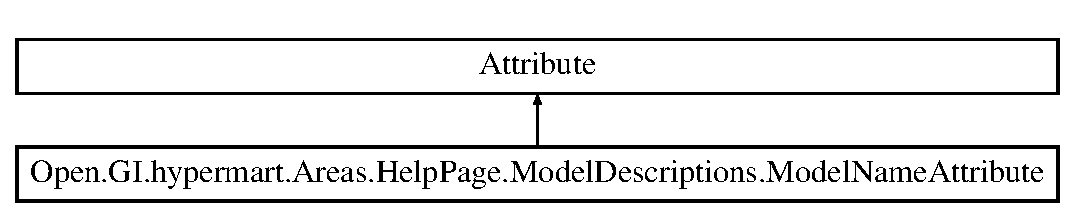
\includegraphics[height=2.000000cm]{class_open_1_1_g_i_1_1hypermart_1_1_areas_1_1_help_page_1_1_model_descriptions_1_1_model_name_attribute}
\end{center}
\end{figure}
\subsection*{Public Member Functions}
\begin{DoxyCompactItemize}
\item 
\hyperlink{class_open_1_1_g_i_1_1hypermart_1_1_areas_1_1_help_page_1_1_model_descriptions_1_1_model_name_attribute_a993a54c4cc771558eef5ea586b70d6d7}{Model\+Name\+Attribute} (string name)
\begin{DoxyCompactList}\small\item\em Initializes a new instance of the \hyperlink{class_open_1_1_g_i_1_1hypermart_1_1_areas_1_1_help_page_1_1_model_descriptions_1_1_model_name_attribute}{Model\+Name\+Attribute} class. \end{DoxyCompactList}\end{DoxyCompactItemize}
\subsection*{Properties}
\begin{DoxyCompactItemize}
\item 
string \hyperlink{class_open_1_1_g_i_1_1hypermart_1_1_areas_1_1_help_page_1_1_model_descriptions_1_1_model_name_attribute_a1388599f97bb13f4b52da9cebfd994d3}{Name}\hspace{0.3cm}{\ttfamily  \mbox{[}get\mbox{]}}
\begin{DoxyCompactList}\small\item\em Gets the name. \end{DoxyCompactList}\end{DoxyCompactItemize}


\subsection{Detailed Description}
Use this attribute to change the name of the \hyperlink{class_open_1_1_g_i_1_1hypermart_1_1_areas_1_1_help_page_1_1_model_descriptions_1_1_model_description}{Model\+Description} generated for a type. 



\subsection{Constructor \& Destructor Documentation}
\hypertarget{class_open_1_1_g_i_1_1hypermart_1_1_areas_1_1_help_page_1_1_model_descriptions_1_1_model_name_attribute_a993a54c4cc771558eef5ea586b70d6d7}{}\label{class_open_1_1_g_i_1_1hypermart_1_1_areas_1_1_help_page_1_1_model_descriptions_1_1_model_name_attribute_a993a54c4cc771558eef5ea586b70d6d7} 
\index{Open\+::\+G\+I\+::hypermart\+::\+Areas\+::\+Help\+Page\+::\+Model\+Descriptions\+::\+Model\+Name\+Attribute@{Open\+::\+G\+I\+::hypermart\+::\+Areas\+::\+Help\+Page\+::\+Model\+Descriptions\+::\+Model\+Name\+Attribute}!Model\+Name\+Attribute@{Model\+Name\+Attribute}}
\index{Model\+Name\+Attribute@{Model\+Name\+Attribute}!Open\+::\+G\+I\+::hypermart\+::\+Areas\+::\+Help\+Page\+::\+Model\+Descriptions\+::\+Model\+Name\+Attribute@{Open\+::\+G\+I\+::hypermart\+::\+Areas\+::\+Help\+Page\+::\+Model\+Descriptions\+::\+Model\+Name\+Attribute}}
\subsubsection{\texorpdfstring{Model\+Name\+Attribute()}{ModelNameAttribute()}}
{\footnotesize\ttfamily Open.\+G\+I.\+hypermart.\+Areas.\+Help\+Page.\+Model\+Descriptions.\+Model\+Name\+Attribute.\+Model\+Name\+Attribute (\begin{DoxyParamCaption}\item[{string}]{name }\end{DoxyParamCaption})}



Initializes a new instance of the \hyperlink{class_open_1_1_g_i_1_1hypermart_1_1_areas_1_1_help_page_1_1_model_descriptions_1_1_model_name_attribute}{Model\+Name\+Attribute} class. 


\begin{DoxyParams}{Parameters}
{\em name} & The name.\\
\hline
\end{DoxyParams}


\subsection{Property Documentation}
\hypertarget{class_open_1_1_g_i_1_1hypermart_1_1_areas_1_1_help_page_1_1_model_descriptions_1_1_model_name_attribute_a1388599f97bb13f4b52da9cebfd994d3}{}\label{class_open_1_1_g_i_1_1hypermart_1_1_areas_1_1_help_page_1_1_model_descriptions_1_1_model_name_attribute_a1388599f97bb13f4b52da9cebfd994d3} 
\index{Open\+::\+G\+I\+::hypermart\+::\+Areas\+::\+Help\+Page\+::\+Model\+Descriptions\+::\+Model\+Name\+Attribute@{Open\+::\+G\+I\+::hypermart\+::\+Areas\+::\+Help\+Page\+::\+Model\+Descriptions\+::\+Model\+Name\+Attribute}!Name@{Name}}
\index{Name@{Name}!Open\+::\+G\+I\+::hypermart\+::\+Areas\+::\+Help\+Page\+::\+Model\+Descriptions\+::\+Model\+Name\+Attribute@{Open\+::\+G\+I\+::hypermart\+::\+Areas\+::\+Help\+Page\+::\+Model\+Descriptions\+::\+Model\+Name\+Attribute}}
\subsubsection{\texorpdfstring{Name}{Name}}
{\footnotesize\ttfamily string Open.\+G\+I.\+hypermart.\+Areas.\+Help\+Page.\+Model\+Descriptions.\+Model\+Name\+Attribute.\+Name\hspace{0.3cm}{\ttfamily [get]}}



Gets the name. 

The name. 

The documentation for this class was generated from the following file\+:\begin{DoxyCompactItemize}
\item 
C\+:/\+Projects/\+App-\/\+Utility-\/\+Store/\+Open.\+G\+I.\+hypermart/\+Areas/\+Help\+Page/\+Model\+Descriptions/\hyperlink{_model_name_attribute_8cs}{Model\+Name\+Attribute.\+cs}\end{DoxyCompactItemize}

\section{Open.\+G\+I.\+hypermart.\+Mvc\+Application Class Reference}
\label{class_open_1_1_g_i_1_1hypermart_1_1_mvc_application}\index{Open.\+G\+I.\+hypermart.\+Mvc\+Application@{Open.\+G\+I.\+hypermart.\+Mvc\+Application}}


Main M\+VC Application Class  


Inheritance diagram for Open.\+G\+I.\+hypermart.\+Mvc\+Application\+:\begin{figure}[H]
\begin{center}
\leavevmode
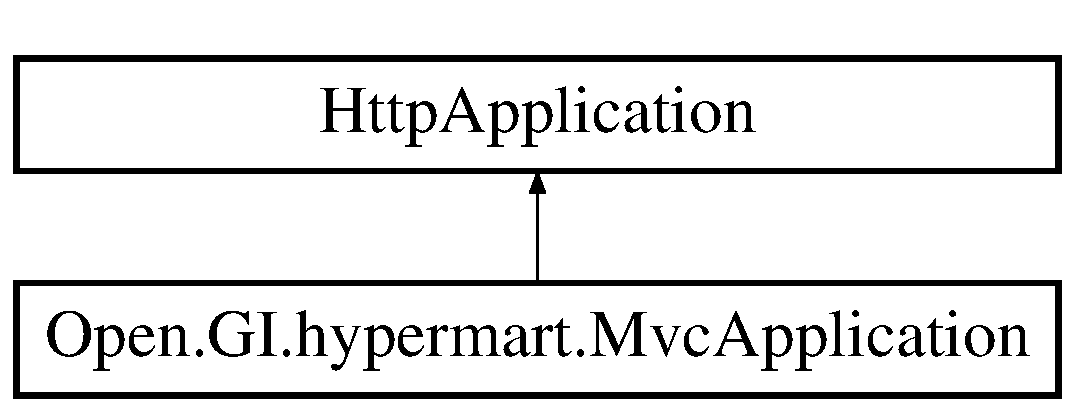
\includegraphics[height=2.000000cm]{class_open_1_1_g_i_1_1hypermart_1_1_mvc_application}
\end{center}
\end{figure}
\subsection*{Protected Member Functions}
\begin{DoxyCompactItemize}
\item 
void \textbf{ Application\+\_\+\+Start} ()
\begin{DoxyCompactList}\small\item\em A\+S\+P.\+N\+ET M\+VC Application start method \end{DoxyCompactList}\end{DoxyCompactItemize}


\subsection{Detailed Description}
Main M\+VC Application Class 

\begin{DoxySeeAlso}{See also}
System.\+Web.\+Http\+Application


\end{DoxySeeAlso}


Definition at line 17 of file Global.\+asax.\+cs.



\subsection{Member Function Documentation}
\mbox{\label{class_open_1_1_g_i_1_1hypermart_1_1_mvc_application_a8169da76cd5c9b98983e4eee8d40ce4e}} 
\index{Open\+::\+G\+I\+::hypermart\+::\+Mvc\+Application@{Open\+::\+G\+I\+::hypermart\+::\+Mvc\+Application}!Application\+\_\+\+Start@{Application\+\_\+\+Start}}
\index{Application\+\_\+\+Start@{Application\+\_\+\+Start}!Open\+::\+G\+I\+::hypermart\+::\+Mvc\+Application@{Open\+::\+G\+I\+::hypermart\+::\+Mvc\+Application}}
\subsubsection{Application\+\_\+\+Start()}
{\footnotesize\ttfamily void Open.\+G\+I.\+hypermart.\+Mvc\+Application.\+Application\+\_\+\+Start (\begin{DoxyParamCaption}{ }\end{DoxyParamCaption})\hspace{0.3cm}{\ttfamily [protected]}}



A\+S\+P.\+N\+ET M\+VC Application start method 



Definition at line 22 of file Global.\+asax.\+cs.



The documentation for this class was generated from the following file\+:\begin{DoxyCompactItemize}
\item 
C\+:/\+Projects/\+App-\/\+Utility-\/\+Store/\+Open.\+G\+I.\+hypermart/\textbf{ Global.\+asax.\+cs}\end{DoxyCompactItemize}

\hypertarget{class_open_1_1_g_i_1_1hypermart_1_1_controllers_1_1_nuget_controller}{}\section{Open.\+G\+I.\+hypermart.\+Controllers.\+Nuget\+Controller Class Reference}
\label{class_open_1_1_g_i_1_1hypermart_1_1_controllers_1_1_nuget_controller}\index{Open.\+G\+I.\+hypermart.\+Controllers.\+Nuget\+Controller@{Open.\+G\+I.\+hypermart.\+Controllers.\+Nuget\+Controller}}


An attempt to create a Nuget controller (phase 2)  


Inheritance diagram for Open.\+G\+I.\+hypermart.\+Controllers.\+Nuget\+Controller\+:\begin{figure}[H]
\begin{center}
\leavevmode
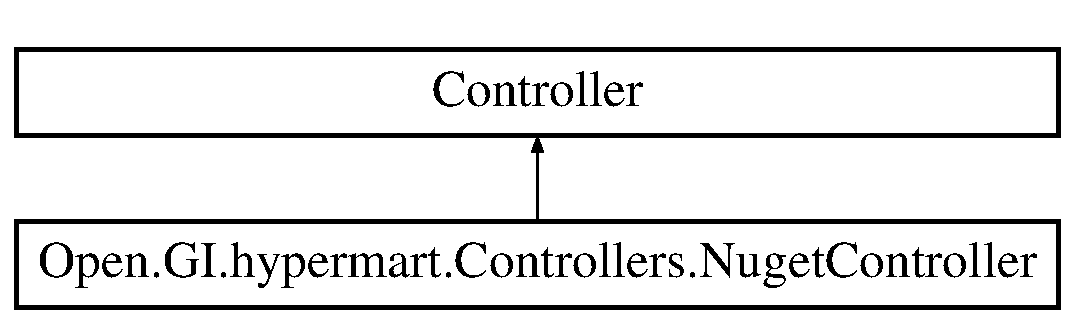
\includegraphics[height=2.000000cm]{class_open_1_1_g_i_1_1hypermart_1_1_controllers_1_1_nuget_controller}
\end{center}
\end{figure}
\subsection*{Public Member Functions}
\begin{DoxyCompactItemize}
\item 
Action\+Result \hyperlink{class_open_1_1_g_i_1_1hypermart_1_1_controllers_1_1_nuget_controller_a4512f0f0edfb480430dea27f009d37a6}{Index} ()
\begin{DoxyCompactList}\small\item\em Indexes this instance. \end{DoxyCompactList}\item 
\hyperlink{class_open_1_1_g_i_1_1hypermart_1_1_helpers_1_1_atom_action_result}{Atom\+Action\+Result} \hyperlink{class_open_1_1_g_i_1_1hypermart_1_1_controllers_1_1_nuget_controller_a8b2f4aa532a73eaacab1efcfd3fed054}{Packages} ()
\begin{DoxyCompactList}\small\item\em Packageses this instance. \end{DoxyCompactList}\end{DoxyCompactItemize}


\subsection{Detailed Description}
An attempt to create a Nuget controller (phase 2) 

\begin{DoxySeeAlso}{See also}
System.\+Web.\+Mvc.\+Controller


\end{DoxySeeAlso}


Definition at line 15 of file Nuget\+Controller.\+cs.



\subsection{Member Function Documentation}
\hypertarget{class_open_1_1_g_i_1_1hypermart_1_1_controllers_1_1_nuget_controller_a4512f0f0edfb480430dea27f009d37a6}{}\index{Open\+::\+G\+I\+::hypermart\+::\+Controllers\+::\+Nuget\+Controller@{Open\+::\+G\+I\+::hypermart\+::\+Controllers\+::\+Nuget\+Controller}!Index@{Index}}
\index{Index@{Index}!Open\+::\+G\+I\+::hypermart\+::\+Controllers\+::\+Nuget\+Controller@{Open\+::\+G\+I\+::hypermart\+::\+Controllers\+::\+Nuget\+Controller}}
\subsubsection[{Index()}]{\setlength{\rightskip}{0pt plus 5cm}Action\+Result Open.\+G\+I.\+hypermart.\+Controllers.\+Nuget\+Controller.\+Index (
\begin{DoxyParamCaption}
{}
\end{DoxyParamCaption}
)}\label{class_open_1_1_g_i_1_1hypermart_1_1_controllers_1_1_nuget_controller_a4512f0f0edfb480430dea27f009d37a6}


Indexes this instance. 

\begin{DoxyReturn}{Returns}

\end{DoxyReturn}


Definition at line 22 of file Nuget\+Controller.\+cs.

\hypertarget{class_open_1_1_g_i_1_1hypermart_1_1_controllers_1_1_nuget_controller_a8b2f4aa532a73eaacab1efcfd3fed054}{}\index{Open\+::\+G\+I\+::hypermart\+::\+Controllers\+::\+Nuget\+Controller@{Open\+::\+G\+I\+::hypermart\+::\+Controllers\+::\+Nuget\+Controller}!Packages@{Packages}}
\index{Packages@{Packages}!Open\+::\+G\+I\+::hypermart\+::\+Controllers\+::\+Nuget\+Controller@{Open\+::\+G\+I\+::hypermart\+::\+Controllers\+::\+Nuget\+Controller}}
\subsubsection[{Packages()}]{\setlength{\rightskip}{0pt plus 5cm}{\bf Atom\+Action\+Result} Open.\+G\+I.\+hypermart.\+Controllers.\+Nuget\+Controller.\+Packages (
\begin{DoxyParamCaption}
{}
\end{DoxyParamCaption}
)}\label{class_open_1_1_g_i_1_1hypermart_1_1_controllers_1_1_nuget_controller_a8b2f4aa532a73eaacab1efcfd3fed054}


Packageses this instance. 

\begin{DoxyReturn}{Returns}

\end{DoxyReturn}


Definition at line 31 of file Nuget\+Controller.\+cs.



The documentation for this class was generated from the following file\+:\begin{DoxyCompactItemize}
\item 
C\+:/\+Projects/\+App-\/\+Utility-\/\+Store/\+Open.\+G\+I.\+hypermart/\+Controllers/\hyperlink{_nuget_controller_8cs}{Nuget\+Controller.\+cs}\end{DoxyCompactItemize}

\hypertarget{class_open_1_1_g_i_1_1hypermart_1_1_areas_1_1_help_page_1_1_object_generator}{}\section{Open.\+G\+I.\+hypermart.\+Areas.\+Help\+Page.\+Object\+Generator Class Reference}
\label{class_open_1_1_g_i_1_1hypermart_1_1_areas_1_1_help_page_1_1_object_generator}\index{Open.\+G\+I.\+hypermart.\+Areas.\+Help\+Page.\+Object\+Generator@{Open.\+G\+I.\+hypermart.\+Areas.\+Help\+Page.\+Object\+Generator}}


This class will create an object of a given type and populate it with sample data.  


\subsection*{Public Member Functions}
\begin{DoxyCompactItemize}
\item 
object \hyperlink{class_open_1_1_g_i_1_1hypermart_1_1_areas_1_1_help_page_1_1_object_generator_a118924d1ff5f565e6e9c2893d36f35d2}{Generate\+Object} (Type type)
\begin{DoxyCompactList}\small\item\em Generates an object for a given type. The type needs to be public, have a public default constructor and settable public properties/fields. Currently it supports the following types\+: Simple types\+: int, string, Enum, Date\+Time, Uri, etc. Complex types\+: P\+O\+C\+O types. Nullables\+: Nullable$<$\+T$>$. Arrays\+: arrays of simple types or complex types. Key value pairs\+: Key\+Value\+Pair$<$\+T\+Key,\+T\+Value$>$ Tuples\+: Tuple$<$\+T1$>$, Tuple$<$\+T1,\+T2$>$, etc Dictionaries\+: I\+Dictionary$<$\+T\+Key,\+T\+Value$>$ or anything deriving from I\+Dictionary$<$\+T\+Key,\+T\+Value$>$. Collections\+: I\+List$<$\+T$>$, I\+Enumerable$<$\+T$>$, I\+Collection$<$\+T$>$, I\+List, I\+Enumerable, I\+Collection or anything deriving from I\+Collection$<$\+T$>$ or I\+List. Queryables\+: I\+Queryable, I\+Queryable$<$\+T$>$. \end{DoxyCompactList}\end{DoxyCompactItemize}


\subsection{Detailed Description}
This class will create an object of a given type and populate it with sample data. 



Definition at line 14 of file Object\+Generator.\+cs.



\subsection{Member Function Documentation}
\hypertarget{class_open_1_1_g_i_1_1hypermart_1_1_areas_1_1_help_page_1_1_object_generator_a118924d1ff5f565e6e9c2893d36f35d2}{}\index{Open\+::\+G\+I\+::hypermart\+::\+Areas\+::\+Help\+Page\+::\+Object\+Generator@{Open\+::\+G\+I\+::hypermart\+::\+Areas\+::\+Help\+Page\+::\+Object\+Generator}!Generate\+Object@{Generate\+Object}}
\index{Generate\+Object@{Generate\+Object}!Open\+::\+G\+I\+::hypermart\+::\+Areas\+::\+Help\+Page\+::\+Object\+Generator@{Open\+::\+G\+I\+::hypermart\+::\+Areas\+::\+Help\+Page\+::\+Object\+Generator}}
\subsubsection[{Generate\+Object(\+Type type)}]{\setlength{\rightskip}{0pt plus 5cm}object Open.\+G\+I.\+hypermart.\+Areas.\+Help\+Page.\+Object\+Generator.\+Generate\+Object (
\begin{DoxyParamCaption}
\item[{Type}]{type}
\end{DoxyParamCaption}
)}\label{class_open_1_1_g_i_1_1hypermart_1_1_areas_1_1_help_page_1_1_object_generator_a118924d1ff5f565e6e9c2893d36f35d2}


Generates an object for a given type. The type needs to be public, have a public default constructor and settable public properties/fields. Currently it supports the following types\+: Simple types\+: int, string, Enum, Date\+Time, Uri, etc. Complex types\+: P\+O\+C\+O types. Nullables\+: Nullable$<$\+T$>$. Arrays\+: arrays of simple types or complex types. Key value pairs\+: Key\+Value\+Pair$<$\+T\+Key,\+T\+Value$>$ Tuples\+: Tuple$<$\+T1$>$, Tuple$<$\+T1,\+T2$>$, etc Dictionaries\+: I\+Dictionary$<$\+T\+Key,\+T\+Value$>$ or anything deriving from I\+Dictionary$<$\+T\+Key,\+T\+Value$>$. Collections\+: I\+List$<$\+T$>$, I\+Enumerable$<$\+T$>$, I\+Collection$<$\+T$>$, I\+List, I\+Enumerable, I\+Collection or anything deriving from I\+Collection$<$\+T$>$ or I\+List. Queryables\+: I\+Queryable, I\+Queryable$<$\+T$>$. 


\begin{DoxyParams}{Parameters}
{\em type} & The type.\\
\hline
\end{DoxyParams}
\begin{DoxyReturn}{Returns}
An object of the given type.
\end{DoxyReturn}


Definition at line 33 of file Object\+Generator.\+cs.



The documentation for this class was generated from the following file\+:\begin{DoxyCompactItemize}
\item 
C\+:/\+Projects/\+App-\/\+Utility-\/\+Store/\+Open.\+G\+I.\+hypermart/\+Areas/\+Help\+Page/\+Sample\+Generation/\hyperlink{_object_generator_8cs}{Object\+Generator.\+cs}\end{DoxyCompactItemize}

\section{Open.\+G\+I.\+hypermart.\+Areas.\+Help\+Page.\+Model\+Descriptions.\+Parameter\+Annotation Class Reference}
\label{class_open_1_1_g_i_1_1hypermart_1_1_areas_1_1_help_page_1_1_model_descriptions_1_1_parameter_annotation}\index{Open.\+G\+I.\+hypermart.\+Areas.\+Help\+Page.\+Model\+Descriptions.\+Parameter\+Annotation@{Open.\+G\+I.\+hypermart.\+Areas.\+Help\+Page.\+Model\+Descriptions.\+Parameter\+Annotation}}


 


\subsection*{Properties}
\begin{DoxyCompactItemize}
\item 
Attribute \textbf{ Annotation\+Attribute}\hspace{0.3cm}{\ttfamily  [get, set]}
\begin{DoxyCompactList}\small\item\em Gets or sets the annotation attribute. \end{DoxyCompactList}\item 
string \textbf{ Documentation}\hspace{0.3cm}{\ttfamily  [get, set]}
\begin{DoxyCompactList}\small\item\em Gets or sets the documentation. \end{DoxyCompactList}\end{DoxyCompactItemize}


\subsection{Detailed Description}




Definition at line 8 of file Parameter\+Annotation.\+cs.



\subsection{Property Documentation}
\mbox{\label{class_open_1_1_g_i_1_1hypermart_1_1_areas_1_1_help_page_1_1_model_descriptions_1_1_parameter_annotation_a53e191aedff647b1d7cd63e2bb2219e0}} 
\index{Open\+::\+G\+I\+::hypermart\+::\+Areas\+::\+Help\+Page\+::\+Model\+Descriptions\+::\+Parameter\+Annotation@{Open\+::\+G\+I\+::hypermart\+::\+Areas\+::\+Help\+Page\+::\+Model\+Descriptions\+::\+Parameter\+Annotation}!Annotation\+Attribute@{Annotation\+Attribute}}
\index{Annotation\+Attribute@{Annotation\+Attribute}!Open\+::\+G\+I\+::hypermart\+::\+Areas\+::\+Help\+Page\+::\+Model\+Descriptions\+::\+Parameter\+Annotation@{Open\+::\+G\+I\+::hypermart\+::\+Areas\+::\+Help\+Page\+::\+Model\+Descriptions\+::\+Parameter\+Annotation}}
\subsubsection{Annotation\+Attribute}
{\footnotesize\ttfamily Attribute Open.\+G\+I.\+hypermart.\+Areas.\+Help\+Page.\+Model\+Descriptions.\+Parameter\+Annotation.\+Annotation\+Attribute\hspace{0.3cm}{\ttfamily [get]}, {\ttfamily [set]}}



Gets or sets the annotation attribute. 

The annotation attribute. 

Definition at line 16 of file Parameter\+Annotation.\+cs.

\mbox{\label{class_open_1_1_g_i_1_1hypermart_1_1_areas_1_1_help_page_1_1_model_descriptions_1_1_parameter_annotation_a9bfcc6f5d41c3630187373bbf9993fa4}} 
\index{Open\+::\+G\+I\+::hypermart\+::\+Areas\+::\+Help\+Page\+::\+Model\+Descriptions\+::\+Parameter\+Annotation@{Open\+::\+G\+I\+::hypermart\+::\+Areas\+::\+Help\+Page\+::\+Model\+Descriptions\+::\+Parameter\+Annotation}!Documentation@{Documentation}}
\index{Documentation@{Documentation}!Open\+::\+G\+I\+::hypermart\+::\+Areas\+::\+Help\+Page\+::\+Model\+Descriptions\+::\+Parameter\+Annotation@{Open\+::\+G\+I\+::hypermart\+::\+Areas\+::\+Help\+Page\+::\+Model\+Descriptions\+::\+Parameter\+Annotation}}
\subsubsection{Documentation}
{\footnotesize\ttfamily string Open.\+G\+I.\+hypermart.\+Areas.\+Help\+Page.\+Model\+Descriptions.\+Parameter\+Annotation.\+Documentation\hspace{0.3cm}{\ttfamily [get]}, {\ttfamily [set]}}



Gets or sets the documentation. 

The documentation. 

Definition at line 24 of file Parameter\+Annotation.\+cs.



The documentation for this class was generated from the following file\+:\begin{DoxyCompactItemize}
\item 
C\+:/\+Projects/\+App-\/\+Utility-\/\+Store/\+Open.\+G\+I.\+hypermart/\+Areas/\+Help\+Page/\+Model\+Descriptions/\textbf{ Parameter\+Annotation.\+cs}\end{DoxyCompactItemize}

\section{Open.\+G\+I.\+hypermart.\+Areas.\+Help\+Page.\+Model\+Descriptions.\+Parameter\+Description Class Reference}
\label{class_open_1_1_g_i_1_1hypermart_1_1_areas_1_1_help_page_1_1_model_descriptions_1_1_parameter_description}\index{Open.\+G\+I.\+hypermart.\+Areas.\+Help\+Page.\+Model\+Descriptions.\+Parameter\+Description@{Open.\+G\+I.\+hypermart.\+Areas.\+Help\+Page.\+Model\+Descriptions.\+Parameter\+Description}}


 


\subsection*{Public Member Functions}
\begin{DoxyCompactItemize}
\item 
\textbf{ Parameter\+Description} ()
\begin{DoxyCompactList}\small\item\em Initializes a new instance of the \doxyref{Parameter\+Description}{p.}{class_open_1_1_g_i_1_1hypermart_1_1_areas_1_1_help_page_1_1_model_descriptions_1_1_parameter_description} class. \end{DoxyCompactList}\end{DoxyCompactItemize}
\subsection*{Properties}
\begin{DoxyCompactItemize}
\item 
Collection$<$ \textbf{ Parameter\+Annotation} $>$ \textbf{ Annotations}\hspace{0.3cm}{\ttfamily  [get]}
\begin{DoxyCompactList}\small\item\em Gets the annotations. \end{DoxyCompactList}\item 
string \textbf{ Documentation}\hspace{0.3cm}{\ttfamily  [get, set]}
\begin{DoxyCompactList}\small\item\em Gets or sets the documentation. \end{DoxyCompactList}\item 
string \textbf{ Name}\hspace{0.3cm}{\ttfamily  [get, set]}
\begin{DoxyCompactList}\small\item\em Gets or sets the name. \end{DoxyCompactList}\item 
\textbf{ Model\+Description} \textbf{ Type\+Description}\hspace{0.3cm}{\ttfamily  [get, set]}
\begin{DoxyCompactList}\small\item\em Gets or sets the type description. \end{DoxyCompactList}\end{DoxyCompactItemize}


\subsection{Detailed Description}




Definition at line 9 of file Parameter\+Description.\+cs.



\subsection{Constructor \& Destructor Documentation}
\mbox{\label{class_open_1_1_g_i_1_1hypermart_1_1_areas_1_1_help_page_1_1_model_descriptions_1_1_parameter_description_a6a431c66f4493e970ceb5477cede9744}} 
\index{Open\+::\+G\+I\+::hypermart\+::\+Areas\+::\+Help\+Page\+::\+Model\+Descriptions\+::\+Parameter\+Description@{Open\+::\+G\+I\+::hypermart\+::\+Areas\+::\+Help\+Page\+::\+Model\+Descriptions\+::\+Parameter\+Description}!Parameter\+Description@{Parameter\+Description}}
\index{Parameter\+Description@{Parameter\+Description}!Open\+::\+G\+I\+::hypermart\+::\+Areas\+::\+Help\+Page\+::\+Model\+Descriptions\+::\+Parameter\+Description@{Open\+::\+G\+I\+::hypermart\+::\+Areas\+::\+Help\+Page\+::\+Model\+Descriptions\+::\+Parameter\+Description}}
\subsubsection{Parameter\+Description()}
{\footnotesize\ttfamily Open.\+G\+I.\+hypermart.\+Areas.\+Help\+Page.\+Model\+Descriptions.\+Parameter\+Description.\+Parameter\+Description (\begin{DoxyParamCaption}{ }\end{DoxyParamCaption})}



Initializes a new instance of the \doxyref{Parameter\+Description}{p.}{class_open_1_1_g_i_1_1hypermart_1_1_areas_1_1_help_page_1_1_model_descriptions_1_1_parameter_description} class. 



Definition at line 14 of file Parameter\+Description.\+cs.



\subsection{Property Documentation}
\mbox{\label{class_open_1_1_g_i_1_1hypermart_1_1_areas_1_1_help_page_1_1_model_descriptions_1_1_parameter_description_ab64b50d81b22dc90c5d40081722ff711}} 
\index{Open\+::\+G\+I\+::hypermart\+::\+Areas\+::\+Help\+Page\+::\+Model\+Descriptions\+::\+Parameter\+Description@{Open\+::\+G\+I\+::hypermart\+::\+Areas\+::\+Help\+Page\+::\+Model\+Descriptions\+::\+Parameter\+Description}!Annotations@{Annotations}}
\index{Annotations@{Annotations}!Open\+::\+G\+I\+::hypermart\+::\+Areas\+::\+Help\+Page\+::\+Model\+Descriptions\+::\+Parameter\+Description@{Open\+::\+G\+I\+::hypermart\+::\+Areas\+::\+Help\+Page\+::\+Model\+Descriptions\+::\+Parameter\+Description}}
\subsubsection{Annotations}
{\footnotesize\ttfamily Collection$<$\textbf{ Parameter\+Annotation}$>$ Open.\+G\+I.\+hypermart.\+Areas.\+Help\+Page.\+Model\+Descriptions.\+Parameter\+Description.\+Annotations\hspace{0.3cm}{\ttfamily [get]}}



Gets the annotations. 

The annotations. 

Definition at line 25 of file Parameter\+Description.\+cs.

\mbox{\label{class_open_1_1_g_i_1_1hypermart_1_1_areas_1_1_help_page_1_1_model_descriptions_1_1_parameter_description_a14b38b56f23972d23b7fc5594b5ac15f}} 
\index{Open\+::\+G\+I\+::hypermart\+::\+Areas\+::\+Help\+Page\+::\+Model\+Descriptions\+::\+Parameter\+Description@{Open\+::\+G\+I\+::hypermart\+::\+Areas\+::\+Help\+Page\+::\+Model\+Descriptions\+::\+Parameter\+Description}!Documentation@{Documentation}}
\index{Documentation@{Documentation}!Open\+::\+G\+I\+::hypermart\+::\+Areas\+::\+Help\+Page\+::\+Model\+Descriptions\+::\+Parameter\+Description@{Open\+::\+G\+I\+::hypermart\+::\+Areas\+::\+Help\+Page\+::\+Model\+Descriptions\+::\+Parameter\+Description}}
\subsubsection{Documentation}
{\footnotesize\ttfamily string Open.\+G\+I.\+hypermart.\+Areas.\+Help\+Page.\+Model\+Descriptions.\+Parameter\+Description.\+Documentation\hspace{0.3cm}{\ttfamily [get]}, {\ttfamily [set]}}



Gets or sets the documentation. 

The documentation. 

Definition at line 33 of file Parameter\+Description.\+cs.

\mbox{\label{class_open_1_1_g_i_1_1hypermart_1_1_areas_1_1_help_page_1_1_model_descriptions_1_1_parameter_description_a213cc3debc198eb331e57e38ecdca4ed}} 
\index{Open\+::\+G\+I\+::hypermart\+::\+Areas\+::\+Help\+Page\+::\+Model\+Descriptions\+::\+Parameter\+Description@{Open\+::\+G\+I\+::hypermart\+::\+Areas\+::\+Help\+Page\+::\+Model\+Descriptions\+::\+Parameter\+Description}!Name@{Name}}
\index{Name@{Name}!Open\+::\+G\+I\+::hypermart\+::\+Areas\+::\+Help\+Page\+::\+Model\+Descriptions\+::\+Parameter\+Description@{Open\+::\+G\+I\+::hypermart\+::\+Areas\+::\+Help\+Page\+::\+Model\+Descriptions\+::\+Parameter\+Description}}
\subsubsection{Name}
{\footnotesize\ttfamily string Open.\+G\+I.\+hypermart.\+Areas.\+Help\+Page.\+Model\+Descriptions.\+Parameter\+Description.\+Name\hspace{0.3cm}{\ttfamily [get]}, {\ttfamily [set]}}



Gets or sets the name. 

The name. 

Definition at line 41 of file Parameter\+Description.\+cs.

\mbox{\label{class_open_1_1_g_i_1_1hypermart_1_1_areas_1_1_help_page_1_1_model_descriptions_1_1_parameter_description_a175a097aa553ad65ae87f136df0e24e7}} 
\index{Open\+::\+G\+I\+::hypermart\+::\+Areas\+::\+Help\+Page\+::\+Model\+Descriptions\+::\+Parameter\+Description@{Open\+::\+G\+I\+::hypermart\+::\+Areas\+::\+Help\+Page\+::\+Model\+Descriptions\+::\+Parameter\+Description}!Type\+Description@{Type\+Description}}
\index{Type\+Description@{Type\+Description}!Open\+::\+G\+I\+::hypermart\+::\+Areas\+::\+Help\+Page\+::\+Model\+Descriptions\+::\+Parameter\+Description@{Open\+::\+G\+I\+::hypermart\+::\+Areas\+::\+Help\+Page\+::\+Model\+Descriptions\+::\+Parameter\+Description}}
\subsubsection{Type\+Description}
{\footnotesize\ttfamily \textbf{ Model\+Description} Open.\+G\+I.\+hypermart.\+Areas.\+Help\+Page.\+Model\+Descriptions.\+Parameter\+Description.\+Type\+Description\hspace{0.3cm}{\ttfamily [get]}, {\ttfamily [set]}}



Gets or sets the type description. 

The type description. 

Definition at line 49 of file Parameter\+Description.\+cs.



The documentation for this class was generated from the following file\+:\begin{DoxyCompactItemize}
\item 
C\+:/\+Projects/\+App-\/\+Utility-\/\+Store/\+Open.\+G\+I.\+hypermart/\+Areas/\+Help\+Page/\+Model\+Descriptions/\textbf{ Parameter\+Description.\+cs}\end{DoxyCompactItemize}

\section{Open.\+G\+I.\+hypermart.\+Models.\+Platform Class Reference}
\label{class_open_1_1_g_i_1_1hypermart_1_1_models_1_1_platform}\index{Open.\+G\+I.\+hypermart.\+Models.\+Platform@{Open.\+G\+I.\+hypermart.\+Models.\+Platform}}


Model Class for platform.  


\subsection*{Public Member Functions}
\begin{DoxyCompactItemize}
\item 
\textbf{ Platform} ()
\begin{DoxyCompactList}\small\item\em Initializes a new instance of the \doxyref{Platform}{p.}{class_open_1_1_g_i_1_1hypermart_1_1_models_1_1_platform} class. \end{DoxyCompactList}\item 
\textbf{ Platform} ()
\end{DoxyCompactItemize}
\subsection*{Properties}
\begin{DoxyCompactItemize}
\item 
string \textbf{ ID}\hspace{0.3cm}{\ttfamily  [get, set]}
\begin{DoxyCompactList}\small\item\em Gets or sets the identifier. \end{DoxyCompactList}\item 
string \textbf{ Platform1}\hspace{0.3cm}{\ttfamily  [get, set]}
\begin{DoxyCompactList}\small\item\em Gets or sets the platform1. \end{DoxyCompactList}\item 
virtual I\+Collection$<$ \textbf{ File} $>$ \textbf{ Files}\hspace{0.3cm}{\ttfamily  [get, set]}
\begin{DoxyCompactList}\small\item\em Gets or sets the files. \end{DoxyCompactList}\item 
virtual I\+Collection$<$ \textbf{ File\+Platform} $>$ \textbf{ File\+Platforms}\hspace{0.3cm}{\ttfamily  [get, set]}
\end{DoxyCompactItemize}


\subsection{Detailed Description}
Model Class for platform. 



Definition at line 12 of file Platform.\+cs.



\subsection{Constructor \& Destructor Documentation}
\mbox{\label{class_open_1_1_g_i_1_1hypermart_1_1_models_1_1_platform_a6c806705f4dc1171773096a5249a1563}} 
\index{Open\+::\+G\+I\+::hypermart\+::\+Models\+::\+Platform@{Open\+::\+G\+I\+::hypermart\+::\+Models\+::\+Platform}!Platform@{Platform}}
\index{Platform@{Platform}!Open\+::\+G\+I\+::hypermart\+::\+Models\+::\+Platform@{Open\+::\+G\+I\+::hypermart\+::\+Models\+::\+Platform}}
\subsubsection{Platform()\hspace{0.1cm}{\footnotesize\ttfamily [1/2]}}
{\footnotesize\ttfamily Open.\+G\+I.\+hypermart.\+Models.\+Platform.\+Platform (\begin{DoxyParamCaption}{ }\end{DoxyParamCaption})}



Initializes a new instance of the \doxyref{Platform}{p.}{class_open_1_1_g_i_1_1hypermart_1_1_models_1_1_platform} class. 



Definition at line 18 of file Platform.\+cs.

\mbox{\label{class_open_1_1_g_i_1_1hypermart_1_1_models_1_1_platform_a6c806705f4dc1171773096a5249a1563}} 
\index{Open\+::\+G\+I\+::hypermart\+::\+Models\+::\+Platform@{Open\+::\+G\+I\+::hypermart\+::\+Models\+::\+Platform}!Platform@{Platform}}
\index{Platform@{Platform}!Open\+::\+G\+I\+::hypermart\+::\+Models\+::\+Platform@{Open\+::\+G\+I\+::hypermart\+::\+Models\+::\+Platform}}
\subsubsection{Platform()\hspace{0.1cm}{\footnotesize\ttfamily [2/2]}}
{\footnotesize\ttfamily Open.\+G\+I.\+hypermart.\+Models.\+Platform.\+Platform (\begin{DoxyParamCaption}{ }\end{DoxyParamCaption})}



Definition at line 18 of file Platform.\+cs.



\subsection{Property Documentation}
\mbox{\label{class_open_1_1_g_i_1_1hypermart_1_1_models_1_1_platform_ac358f8b1b556f6d99fb47fdb29de7202}} 
\index{Open\+::\+G\+I\+::hypermart\+::\+Models\+::\+Platform@{Open\+::\+G\+I\+::hypermart\+::\+Models\+::\+Platform}!File\+Platforms@{File\+Platforms}}
\index{File\+Platforms@{File\+Platforms}!Open\+::\+G\+I\+::hypermart\+::\+Models\+::\+Platform@{Open\+::\+G\+I\+::hypermart\+::\+Models\+::\+Platform}}
\subsubsection{File\+Platforms}
{\footnotesize\ttfamily virtual I\+Collection$<$\textbf{ File\+Platform}$>$ Open.\+G\+I.\+hypermart.\+Models.\+Platform.\+File\+Platforms\hspace{0.3cm}{\ttfamily [get]}, {\ttfamily [set]}}



Definition at line 27 of file Platform.\+cs.

\mbox{\label{class_open_1_1_g_i_1_1hypermart_1_1_models_1_1_platform_a984a31b30ada1f33acef9099c09d9ca0}} 
\index{Open\+::\+G\+I\+::hypermart\+::\+Models\+::\+Platform@{Open\+::\+G\+I\+::hypermart\+::\+Models\+::\+Platform}!Files@{Files}}
\index{Files@{Files}!Open\+::\+G\+I\+::hypermart\+::\+Models\+::\+Platform@{Open\+::\+G\+I\+::hypermart\+::\+Models\+::\+Platform}}
\subsubsection{Files}
{\footnotesize\ttfamily virtual I\+Collection$<$\textbf{ File}$>$ Open.\+G\+I.\+hypermart.\+Models.\+Platform.\+Files\hspace{0.3cm}{\ttfamily [get]}, {\ttfamily [set]}}



Gets or sets the files. 

The files. 

Definition at line 47 of file Platform.\+cs.

\mbox{\label{class_open_1_1_g_i_1_1hypermart_1_1_models_1_1_platform_ae11ad27de467131d539e35f598ff3051}} 
\index{Open\+::\+G\+I\+::hypermart\+::\+Models\+::\+Platform@{Open\+::\+G\+I\+::hypermart\+::\+Models\+::\+Platform}!ID@{ID}}
\index{ID@{ID}!Open\+::\+G\+I\+::hypermart\+::\+Models\+::\+Platform@{Open\+::\+G\+I\+::hypermart\+::\+Models\+::\+Platform}}
\subsubsection{ID}
{\footnotesize\ttfamily string Open.\+G\+I.\+hypermart.\+Models.\+Platform.\+ID\hspace{0.3cm}{\ttfamily [get]}, {\ttfamily [set]}}



Gets or sets the identifier. 

The identifier. 

Definition at line 30 of file Platform.\+cs.

\mbox{\label{class_open_1_1_g_i_1_1hypermart_1_1_models_1_1_platform_aa93619cbb18655b2425f416df0f194c6}} 
\index{Open\+::\+G\+I\+::hypermart\+::\+Models\+::\+Platform@{Open\+::\+G\+I\+::hypermart\+::\+Models\+::\+Platform}!Platform1@{Platform1}}
\index{Platform1@{Platform1}!Open\+::\+G\+I\+::hypermart\+::\+Models\+::\+Platform@{Open\+::\+G\+I\+::hypermart\+::\+Models\+::\+Platform}}
\subsubsection{Platform1}
{\footnotesize\ttfamily string Open.\+G\+I.\+hypermart.\+Models.\+Platform.\+Platform1\hspace{0.3cm}{\ttfamily [get]}, {\ttfamily [set]}}



Gets or sets the platform1. 

The platform1. 

Definition at line 38 of file Platform.\+cs.



The documentation for this class was generated from the following file\+:\begin{DoxyCompactItemize}
\item 
C\+:/\+Projects/\+App-\/\+Utility-\/\+Store/\+Open.\+G\+I.\+hypermart/\+Models/\textbf{ Platform.\+cs}\end{DoxyCompactItemize}

\hypertarget{class_open_1_1_g_i_1_1hypermart_1_1_models_1_1_product}{}\section{Open.\+G\+I.\+hypermart.\+Models.\+Product Class Reference}
\label{class_open_1_1_g_i_1_1hypermart_1_1_models_1_1_product}\index{Open.\+G\+I.\+hypermart.\+Models.\+Product@{Open.\+G\+I.\+hypermart.\+Models.\+Product}}


\hyperlink{class_open_1_1_g_i_1_1hypermart_1_1_models_1_1_product}{Product} Model Class  


\subsection*{Public Member Functions}
\begin{DoxyCompactItemize}
\item 
\hyperlink{class_open_1_1_g_i_1_1hypermart_1_1_models_1_1_product_a6e3b824c07f190baa506f9c73da63e62}{Product} ()
\begin{DoxyCompactList}\small\item\em Initializes a new instance of the \hyperlink{class_open_1_1_g_i_1_1hypermart_1_1_models_1_1_product}{Product} class. \end{DoxyCompactList}\item 
\hyperlink{class_open_1_1_g_i_1_1hypermart_1_1_models_1_1_product_a6e3b824c07f190baa506f9c73da63e62}{Product} ()
\end{DoxyCompactItemize}
\subsection*{Properties}
\begin{DoxyCompactItemize}
\item 
int \hyperlink{class_open_1_1_g_i_1_1hypermart_1_1_models_1_1_product_a4fedd3f62a9c36939c6e45ea2e8cd011}{I\+D}\hspace{0.3cm}{\ttfamily  \mbox{[}get, set\mbox{]}}
\begin{DoxyCompactList}\small\item\em Gets or sets the identifier. \end{DoxyCompactList}\item 
string \hyperlink{class_open_1_1_g_i_1_1hypermart_1_1_models_1_1_product_a877241a61c423e91b6b630df5ca811d0}{Title}\hspace{0.3cm}{\ttfamily  \mbox{[}get, set\mbox{]}}
\begin{DoxyCompactList}\small\item\em Gets or sets the title. \end{DoxyCompactList}\item 
string \hyperlink{class_open_1_1_g_i_1_1hypermart_1_1_models_1_1_product_a8d7cb8cd22f77fa66f06726400b1381e}{Description}\hspace{0.3cm}{\ttfamily  \mbox{[}get, set\mbox{]}}
\begin{DoxyCompactList}\small\item\em Gets or sets the description. \end{DoxyCompactList}\item 
string \hyperlink{class_open_1_1_g_i_1_1hypermart_1_1_models_1_1_product_ad0233eb35ac4048277a4eafde6432c43}{Tagline}\hspace{0.3cm}{\ttfamily  \mbox{[}get, set\mbox{]}}
\begin{DoxyCompactList}\small\item\em Gets or sets the tagline. \end{DoxyCompactList}\item 
string \hyperlink{class_open_1_1_g_i_1_1hypermart_1_1_models_1_1_product_a646bc5e183ba8d87c06d290398e6bee6}{Lead}\hspace{0.3cm}{\ttfamily  \mbox{[}get, set\mbox{]}}
\begin{DoxyCompactList}\small\item\em Gets or sets the lead. \end{DoxyCompactList}\item 
string \hyperlink{class_open_1_1_g_i_1_1hypermart_1_1_models_1_1_product_ab5fd5620220d0e68053208859137a6cb}{Source\+Code}\hspace{0.3cm}{\ttfamily  \mbox{[}get, set\mbox{]}}
\begin{DoxyCompactList}\small\item\em Gets or sets the source code location for the project. \end{DoxyCompactList}\item 
virtual I\+Collection$<$ string $>$ \hyperlink{class_open_1_1_g_i_1_1hypermart_1_1_models_1_1_product_af39b6e12bee2265db7bbca5ecbeb116c}{Maintainers}\hspace{0.3cm}{\ttfamily  \mbox{[}get, set\mbox{]}}
\begin{DoxyCompactList}\small\item\em Gets or sets the maintainers. \end{DoxyCompactList}\item 
virtual I\+Collection$<$ \hyperlink{class_open_1_1_g_i_1_1hypermart_1_1_models_1_1_file}{File} $>$ \hyperlink{class_open_1_1_g_i_1_1hypermart_1_1_models_1_1_product_a8632e80d5f05c8818c289b3924137c13}{Files}\hspace{0.3cm}{\ttfamily  \mbox{[}get, set\mbox{]}}
\begin{DoxyCompactList}\small\item\em Gets or sets the files. \end{DoxyCompactList}\item 
virtual I\+Collection$<$ \hyperlink{class_open_1_1_g_i_1_1hypermart_1_1_models_1_1_screenshot}{Screenshot} $>$ \hyperlink{class_open_1_1_g_i_1_1hypermart_1_1_models_1_1_product_a5fae1aafb8f9a3af27ce369d5d053df1}{Screenshots}\hspace{0.3cm}{\ttfamily  \mbox{[}get, set\mbox{]}}
\begin{DoxyCompactList}\small\item\em Gets or sets the screenshots. \end{DoxyCompactList}\end{DoxyCompactItemize}


\subsection{Detailed Description}
\hyperlink{class_open_1_1_g_i_1_1hypermart_1_1_models_1_1_product}{Product} Model Class 



Definition at line 12 of file Product.\+cs.



\subsection{Constructor \& Destructor Documentation}
\hypertarget{class_open_1_1_g_i_1_1hypermart_1_1_models_1_1_product_a6e3b824c07f190baa506f9c73da63e62}{}\index{Open\+::\+G\+I\+::hypermart\+::\+Models\+::\+Product@{Open\+::\+G\+I\+::hypermart\+::\+Models\+::\+Product}!Product@{Product}}
\index{Product@{Product}!Open\+::\+G\+I\+::hypermart\+::\+Models\+::\+Product@{Open\+::\+G\+I\+::hypermart\+::\+Models\+::\+Product}}
\subsubsection[{Product()}]{\setlength{\rightskip}{0pt plus 5cm}Open.\+G\+I.\+hypermart.\+Models.\+Product.\+Product (
\begin{DoxyParamCaption}
{}
\end{DoxyParamCaption}
)}\label{class_open_1_1_g_i_1_1hypermart_1_1_models_1_1_product_a6e3b824c07f190baa506f9c73da63e62}


Initializes a new instance of the \hyperlink{class_open_1_1_g_i_1_1hypermart_1_1_models_1_1_product}{Product} class. 



Definition at line 18 of file Product.\+cs.

\hypertarget{class_open_1_1_g_i_1_1hypermart_1_1_models_1_1_product_a6e3b824c07f190baa506f9c73da63e62}{}\index{Open\+::\+G\+I\+::hypermart\+::\+Models\+::\+Product@{Open\+::\+G\+I\+::hypermart\+::\+Models\+::\+Product}!Product@{Product}}
\index{Product@{Product}!Open\+::\+G\+I\+::hypermart\+::\+Models\+::\+Product@{Open\+::\+G\+I\+::hypermart\+::\+Models\+::\+Product}}
\subsubsection[{Product()}]{\setlength{\rightskip}{0pt plus 5cm}Open.\+G\+I.\+hypermart.\+Models.\+Product.\+Product (
\begin{DoxyParamCaption}
{}
\end{DoxyParamCaption}
)}\label{class_open_1_1_g_i_1_1hypermart_1_1_models_1_1_product_a6e3b824c07f190baa506f9c73da63e62}


Definition at line 18 of file Product.\+cs.



\subsection{Property Documentation}
\hypertarget{class_open_1_1_g_i_1_1hypermart_1_1_models_1_1_product_a8d7cb8cd22f77fa66f06726400b1381e}{}\index{Open\+::\+G\+I\+::hypermart\+::\+Models\+::\+Product@{Open\+::\+G\+I\+::hypermart\+::\+Models\+::\+Product}!Description@{Description}}
\index{Description@{Description}!Open\+::\+G\+I\+::hypermart\+::\+Models\+::\+Product@{Open\+::\+G\+I\+::hypermart\+::\+Models\+::\+Product}}
\subsubsection[{Description}]{\setlength{\rightskip}{0pt plus 5cm}string Open.\+G\+I.\+hypermart.\+Models.\+Product.\+Description\hspace{0.3cm}{\ttfamily [get]}, {\ttfamily [set]}}\label{class_open_1_1_g_i_1_1hypermart_1_1_models_1_1_product_a8d7cb8cd22f77fa66f06726400b1381e}


Gets or sets the description. 

The description. 

Definition at line 46 of file Product.\+cs.

\hypertarget{class_open_1_1_g_i_1_1hypermart_1_1_models_1_1_product_a8632e80d5f05c8818c289b3924137c13}{}\index{Open\+::\+G\+I\+::hypermart\+::\+Models\+::\+Product@{Open\+::\+G\+I\+::hypermart\+::\+Models\+::\+Product}!Files@{Files}}
\index{Files@{Files}!Open\+::\+G\+I\+::hypermart\+::\+Models\+::\+Product@{Open\+::\+G\+I\+::hypermart\+::\+Models\+::\+Product}}
\subsubsection[{Files}]{\setlength{\rightskip}{0pt plus 5cm}I\+Collection$<$ {\bf File} $>$ Open.\+G\+I.\+hypermart.\+Models.\+Product.\+Files\hspace{0.3cm}{\ttfamily [get]}, {\ttfamily [set]}}\label{class_open_1_1_g_i_1_1hypermart_1_1_models_1_1_product_a8632e80d5f05c8818c289b3924137c13}


Gets or sets the files. 

The files. 

Definition at line 90 of file Product.\+cs.

\hypertarget{class_open_1_1_g_i_1_1hypermart_1_1_models_1_1_product_a4fedd3f62a9c36939c6e45ea2e8cd011}{}\index{Open\+::\+G\+I\+::hypermart\+::\+Models\+::\+Product@{Open\+::\+G\+I\+::hypermart\+::\+Models\+::\+Product}!I\+D@{I\+D}}
\index{I\+D@{I\+D}!Open\+::\+G\+I\+::hypermart\+::\+Models\+::\+Product@{Open\+::\+G\+I\+::hypermart\+::\+Models\+::\+Product}}
\subsubsection[{I\+D}]{\setlength{\rightskip}{0pt plus 5cm}int Open.\+G\+I.\+hypermart.\+Models.\+Product.\+I\+D\hspace{0.3cm}{\ttfamily [get]}, {\ttfamily [set]}}\label{class_open_1_1_g_i_1_1hypermart_1_1_models_1_1_product_a4fedd3f62a9c36939c6e45ea2e8cd011}


Gets or sets the identifier. 

The identifier. 

Definition at line 30 of file Product.\+cs.

\hypertarget{class_open_1_1_g_i_1_1hypermart_1_1_models_1_1_product_a646bc5e183ba8d87c06d290398e6bee6}{}\index{Open\+::\+G\+I\+::hypermart\+::\+Models\+::\+Product@{Open\+::\+G\+I\+::hypermart\+::\+Models\+::\+Product}!Lead@{Lead}}
\index{Lead@{Lead}!Open\+::\+G\+I\+::hypermart\+::\+Models\+::\+Product@{Open\+::\+G\+I\+::hypermart\+::\+Models\+::\+Product}}
\subsubsection[{Lead}]{\setlength{\rightskip}{0pt plus 5cm}string Open.\+G\+I.\+hypermart.\+Models.\+Product.\+Lead\hspace{0.3cm}{\ttfamily [get]}, {\ttfamily [set]}}\label{class_open_1_1_g_i_1_1hypermart_1_1_models_1_1_product_a646bc5e183ba8d87c06d290398e6bee6}


Gets or sets the lead. 

The lead. 

Definition at line 63 of file Product.\+cs.

\hypertarget{class_open_1_1_g_i_1_1hypermart_1_1_models_1_1_product_af39b6e12bee2265db7bbca5ecbeb116c}{}\index{Open\+::\+G\+I\+::hypermart\+::\+Models\+::\+Product@{Open\+::\+G\+I\+::hypermart\+::\+Models\+::\+Product}!Maintainers@{Maintainers}}
\index{Maintainers@{Maintainers}!Open\+::\+G\+I\+::hypermart\+::\+Models\+::\+Product@{Open\+::\+G\+I\+::hypermart\+::\+Models\+::\+Product}}
\subsubsection[{Maintainers}]{\setlength{\rightskip}{0pt plus 5cm}virtual I\+Collection$<$string$>$ Open.\+G\+I.\+hypermart.\+Models.\+Product.\+Maintainers\hspace{0.3cm}{\ttfamily [get]}, {\ttfamily [set]}}\label{class_open_1_1_g_i_1_1hypermart_1_1_models_1_1_product_af39b6e12bee2265db7bbca5ecbeb116c}


Gets or sets the maintainers. 

The maintainers. 

Definition at line 80 of file Product.\+cs.

\hypertarget{class_open_1_1_g_i_1_1hypermart_1_1_models_1_1_product_a5fae1aafb8f9a3af27ce369d5d053df1}{}\index{Open\+::\+G\+I\+::hypermart\+::\+Models\+::\+Product@{Open\+::\+G\+I\+::hypermart\+::\+Models\+::\+Product}!Screenshots@{Screenshots}}
\index{Screenshots@{Screenshots}!Open\+::\+G\+I\+::hypermart\+::\+Models\+::\+Product@{Open\+::\+G\+I\+::hypermart\+::\+Models\+::\+Product}}
\subsubsection[{Screenshots}]{\setlength{\rightskip}{0pt plus 5cm}I\+Collection$<$ {\bf Screenshot} $>$ Open.\+G\+I.\+hypermart.\+Models.\+Product.\+Screenshots\hspace{0.3cm}{\ttfamily [get]}, {\ttfamily [set]}}\label{class_open_1_1_g_i_1_1hypermart_1_1_models_1_1_product_a5fae1aafb8f9a3af27ce369d5d053df1}


Gets or sets the screenshots. 

The screenshots. 

Definition at line 99 of file Product.\+cs.

\hypertarget{class_open_1_1_g_i_1_1hypermart_1_1_models_1_1_product_ab5fd5620220d0e68053208859137a6cb}{}\index{Open\+::\+G\+I\+::hypermart\+::\+Models\+::\+Product@{Open\+::\+G\+I\+::hypermart\+::\+Models\+::\+Product}!Source\+Code@{Source\+Code}}
\index{Source\+Code@{Source\+Code}!Open\+::\+G\+I\+::hypermart\+::\+Models\+::\+Product@{Open\+::\+G\+I\+::hypermart\+::\+Models\+::\+Product}}
\subsubsection[{Source\+Code}]{\setlength{\rightskip}{0pt plus 5cm}string Open.\+G\+I.\+hypermart.\+Models.\+Product.\+Source\+Code\hspace{0.3cm}{\ttfamily [get]}, {\ttfamily [set]}}\label{class_open_1_1_g_i_1_1hypermart_1_1_models_1_1_product_ab5fd5620220d0e68053208859137a6cb}


Gets or sets the source code location for the project. 

The source code. 

Definition at line 71 of file Product.\+cs.

\hypertarget{class_open_1_1_g_i_1_1hypermart_1_1_models_1_1_product_ad0233eb35ac4048277a4eafde6432c43}{}\index{Open\+::\+G\+I\+::hypermart\+::\+Models\+::\+Product@{Open\+::\+G\+I\+::hypermart\+::\+Models\+::\+Product}!Tagline@{Tagline}}
\index{Tagline@{Tagline}!Open\+::\+G\+I\+::hypermart\+::\+Models\+::\+Product@{Open\+::\+G\+I\+::hypermart\+::\+Models\+::\+Product}}
\subsubsection[{Tagline}]{\setlength{\rightskip}{0pt plus 5cm}string Open.\+G\+I.\+hypermart.\+Models.\+Product.\+Tagline\hspace{0.3cm}{\ttfamily [get]}, {\ttfamily [set]}}\label{class_open_1_1_g_i_1_1hypermart_1_1_models_1_1_product_ad0233eb35ac4048277a4eafde6432c43}


Gets or sets the tagline. 

The tagline. 

Definition at line 54 of file Product.\+cs.

\hypertarget{class_open_1_1_g_i_1_1hypermart_1_1_models_1_1_product_a877241a61c423e91b6b630df5ca811d0}{}\index{Open\+::\+G\+I\+::hypermart\+::\+Models\+::\+Product@{Open\+::\+G\+I\+::hypermart\+::\+Models\+::\+Product}!Title@{Title}}
\index{Title@{Title}!Open\+::\+G\+I\+::hypermart\+::\+Models\+::\+Product@{Open\+::\+G\+I\+::hypermart\+::\+Models\+::\+Product}}
\subsubsection[{Title}]{\setlength{\rightskip}{0pt plus 5cm}string Open.\+G\+I.\+hypermart.\+Models.\+Product.\+Title\hspace{0.3cm}{\ttfamily [get]}, {\ttfamily [set]}}\label{class_open_1_1_g_i_1_1hypermart_1_1_models_1_1_product_a877241a61c423e91b6b630df5ca811d0}


Gets or sets the title. 

The title. 

Definition at line 38 of file Product.\+cs.



The documentation for this class was generated from the following file\+:\begin{DoxyCompactItemize}
\item 
C\+:/\+Projects/\+App-\/\+Utility-\/\+Store/\+Open.\+G\+I.\+hypermart/\+Models/\hyperlink{_models_2_product_8cs}{Product.\+cs}\end{DoxyCompactItemize}

\section{Open.\+G\+I.\+hypermart.\+Data\+Transformation\+Objects.\+Product\+D\+TO Class Reference}
\label{class_open_1_1_g_i_1_1hypermart_1_1_data_transformation_objects_1_1_product_d_t_o}\index{Open.\+G\+I.\+hypermart.\+Data\+Transformation\+Objects.\+Product\+D\+TO@{Open.\+G\+I.\+hypermart.\+Data\+Transformation\+Objects.\+Product\+D\+TO}}


 


\subsection*{Public Member Functions}
\begin{DoxyCompactItemize}
\item 
\textbf{ Product\+D\+TO} ()
\begin{DoxyCompactList}\small\item\em Initializes a new instance of the \doxyref{Product\+D\+TO}{p.}{class_open_1_1_g_i_1_1hypermart_1_1_data_transformation_objects_1_1_product_d_t_o} class. \end{DoxyCompactList}\item 
\textbf{ Product\+D\+TO} (\textbf{ Product} prod)
\begin{DoxyCompactList}\small\item\em Initializes a new instance of the \doxyref{Product\+D\+TO}{p.}{class_open_1_1_g_i_1_1hypermart_1_1_data_transformation_objects_1_1_product_d_t_o} class. \end{DoxyCompactList}\end{DoxyCompactItemize}
\subsection*{Properties}
\begin{DoxyCompactItemize}
\item 
int \textbf{ ID}\hspace{0.3cm}{\ttfamily  [get, set]}
\begin{DoxyCompactList}\small\item\em Gets or sets the identifier. \end{DoxyCompactList}\item 
string \textbf{ Title}\hspace{0.3cm}{\ttfamily  [get, set]}
\begin{DoxyCompactList}\small\item\em Gets or sets the title. \end{DoxyCompactList}\item 
string \textbf{ Description}\hspace{0.3cm}{\ttfamily  [get, set]}
\begin{DoxyCompactList}\small\item\em Gets or sets the description. \end{DoxyCompactList}\item 
string \textbf{ Tagline}\hspace{0.3cm}{\ttfamily  [get, set]}
\begin{DoxyCompactList}\small\item\em Gets or sets the tagline. \end{DoxyCompactList}\item 
string \textbf{ Lead}\hspace{0.3cm}{\ttfamily  [get, set]}
\begin{DoxyCompactList}\small\item\em Gets or sets the lead. \end{DoxyCompactList}\item 
List$<$ byte[$\,$]$>$ \textbf{ Screen\+Shot}\hspace{0.3cm}{\ttfamily  [get, set]}
\begin{DoxyCompactList}\small\item\em Screen Shot \end{DoxyCompactList}\end{DoxyCompactItemize}


\subsection{Detailed Description}




Definition at line 13 of file Product\+D\+T\+O.\+cs.



\subsection{Constructor \& Destructor Documentation}
\mbox{\label{class_open_1_1_g_i_1_1hypermart_1_1_data_transformation_objects_1_1_product_d_t_o_a99130c4316beb76caa542b78f0de4e38}} 
\index{Open\+::\+G\+I\+::hypermart\+::\+Data\+Transformation\+Objects\+::\+Product\+D\+TO@{Open\+::\+G\+I\+::hypermart\+::\+Data\+Transformation\+Objects\+::\+Product\+D\+TO}!Product\+D\+TO@{Product\+D\+TO}}
\index{Product\+D\+TO@{Product\+D\+TO}!Open\+::\+G\+I\+::hypermart\+::\+Data\+Transformation\+Objects\+::\+Product\+D\+TO@{Open\+::\+G\+I\+::hypermart\+::\+Data\+Transformation\+Objects\+::\+Product\+D\+TO}}
\subsubsection{Product\+D\+T\+O()\hspace{0.1cm}{\footnotesize\ttfamily [1/2]}}
{\footnotesize\ttfamily Open.\+G\+I.\+hypermart.\+Data\+Transformation\+Objects.\+Product\+D\+T\+O.\+Product\+D\+TO (\begin{DoxyParamCaption}{ }\end{DoxyParamCaption})}



Initializes a new instance of the \doxyref{Product\+D\+TO}{p.}{class_open_1_1_g_i_1_1hypermart_1_1_data_transformation_objects_1_1_product_d_t_o} class. 



Definition at line 18 of file Product\+D\+T\+O.\+cs.

\mbox{\label{class_open_1_1_g_i_1_1hypermart_1_1_data_transformation_objects_1_1_product_d_t_o_a4deb78b33f6f3fc07ec2d4f49ada1f93}} 
\index{Open\+::\+G\+I\+::hypermart\+::\+Data\+Transformation\+Objects\+::\+Product\+D\+TO@{Open\+::\+G\+I\+::hypermart\+::\+Data\+Transformation\+Objects\+::\+Product\+D\+TO}!Product\+D\+TO@{Product\+D\+TO}}
\index{Product\+D\+TO@{Product\+D\+TO}!Open\+::\+G\+I\+::hypermart\+::\+Data\+Transformation\+Objects\+::\+Product\+D\+TO@{Open\+::\+G\+I\+::hypermart\+::\+Data\+Transformation\+Objects\+::\+Product\+D\+TO}}
\subsubsection{Product\+D\+T\+O()\hspace{0.1cm}{\footnotesize\ttfamily [2/2]}}
{\footnotesize\ttfamily Open.\+G\+I.\+hypermart.\+Data\+Transformation\+Objects.\+Product\+D\+T\+O.\+Product\+D\+TO (\begin{DoxyParamCaption}\item[{\textbf{ Product}}]{prod }\end{DoxyParamCaption})}



Initializes a new instance of the \doxyref{Product\+D\+TO}{p.}{class_open_1_1_g_i_1_1hypermart_1_1_data_transformation_objects_1_1_product_d_t_o} class. 


\begin{DoxyParams}{Parameters}
{\em prod} & The base.\\
\hline
\end{DoxyParams}


Definition at line 26 of file Product\+D\+T\+O.\+cs.



\subsection{Property Documentation}
\mbox{\label{class_open_1_1_g_i_1_1hypermart_1_1_data_transformation_objects_1_1_product_d_t_o_a1de153f9a50688af8c97932d30056fef}} 
\index{Open\+::\+G\+I\+::hypermart\+::\+Data\+Transformation\+Objects\+::\+Product\+D\+TO@{Open\+::\+G\+I\+::hypermart\+::\+Data\+Transformation\+Objects\+::\+Product\+D\+TO}!Description@{Description}}
\index{Description@{Description}!Open\+::\+G\+I\+::hypermart\+::\+Data\+Transformation\+Objects\+::\+Product\+D\+TO@{Open\+::\+G\+I\+::hypermart\+::\+Data\+Transformation\+Objects\+::\+Product\+D\+TO}}
\subsubsection{Description}
{\footnotesize\ttfamily string Open.\+G\+I.\+hypermart.\+Data\+Transformation\+Objects.\+Product\+D\+T\+O.\+Description\hspace{0.3cm}{\ttfamily [get]}, {\ttfamily [set]}}



Gets or sets the description. 

The description. 

Definition at line 62 of file Product\+D\+T\+O.\+cs.

\mbox{\label{class_open_1_1_g_i_1_1hypermart_1_1_data_transformation_objects_1_1_product_d_t_o_ab965f0f2be3b04afb1de5e8fa97cd93a}} 
\index{Open\+::\+G\+I\+::hypermart\+::\+Data\+Transformation\+Objects\+::\+Product\+D\+TO@{Open\+::\+G\+I\+::hypermart\+::\+Data\+Transformation\+Objects\+::\+Product\+D\+TO}!ID@{ID}}
\index{ID@{ID}!Open\+::\+G\+I\+::hypermart\+::\+Data\+Transformation\+Objects\+::\+Product\+D\+TO@{Open\+::\+G\+I\+::hypermart\+::\+Data\+Transformation\+Objects\+::\+Product\+D\+TO}}
\subsubsection{ID}
{\footnotesize\ttfamily int Open.\+G\+I.\+hypermart.\+Data\+Transformation\+Objects.\+Product\+D\+T\+O.\+ID\hspace{0.3cm}{\ttfamily [get]}, {\ttfamily [set]}}



Gets or sets the identifier. 

The identifier. 

Definition at line 46 of file Product\+D\+T\+O.\+cs.

\mbox{\label{class_open_1_1_g_i_1_1hypermart_1_1_data_transformation_objects_1_1_product_d_t_o_a900af3a5017cf99ef7a51c8a496289cc}} 
\index{Open\+::\+G\+I\+::hypermart\+::\+Data\+Transformation\+Objects\+::\+Product\+D\+TO@{Open\+::\+G\+I\+::hypermart\+::\+Data\+Transformation\+Objects\+::\+Product\+D\+TO}!Lead@{Lead}}
\index{Lead@{Lead}!Open\+::\+G\+I\+::hypermart\+::\+Data\+Transformation\+Objects\+::\+Product\+D\+TO@{Open\+::\+G\+I\+::hypermart\+::\+Data\+Transformation\+Objects\+::\+Product\+D\+TO}}
\subsubsection{Lead}
{\footnotesize\ttfamily string Open.\+G\+I.\+hypermart.\+Data\+Transformation\+Objects.\+Product\+D\+T\+O.\+Lead\hspace{0.3cm}{\ttfamily [get]}, {\ttfamily [set]}}



Gets or sets the lead. 

The lead. 

Definition at line 79 of file Product\+D\+T\+O.\+cs.

\mbox{\label{class_open_1_1_g_i_1_1hypermart_1_1_data_transformation_objects_1_1_product_d_t_o_ac2f998445710bc55481fe5983ed485de}} 
\index{Open\+::\+G\+I\+::hypermart\+::\+Data\+Transformation\+Objects\+::\+Product\+D\+TO@{Open\+::\+G\+I\+::hypermart\+::\+Data\+Transformation\+Objects\+::\+Product\+D\+TO}!Screen\+Shot@{Screen\+Shot}}
\index{Screen\+Shot@{Screen\+Shot}!Open\+::\+G\+I\+::hypermart\+::\+Data\+Transformation\+Objects\+::\+Product\+D\+TO@{Open\+::\+G\+I\+::hypermart\+::\+Data\+Transformation\+Objects\+::\+Product\+D\+TO}}
\subsubsection{Screen\+Shot}
{\footnotesize\ttfamily List$<$byte[$\,$]$>$ Open.\+G\+I.\+hypermart.\+Data\+Transformation\+Objects.\+Product\+D\+T\+O.\+Screen\+Shot\hspace{0.3cm}{\ttfamily [get]}, {\ttfamily [set]}}



Screen Shot 



Definition at line 84 of file Product\+D\+T\+O.\+cs.

\mbox{\label{class_open_1_1_g_i_1_1hypermart_1_1_data_transformation_objects_1_1_product_d_t_o_a7b9cf190d3a304a72287dc1c0200aa94}} 
\index{Open\+::\+G\+I\+::hypermart\+::\+Data\+Transformation\+Objects\+::\+Product\+D\+TO@{Open\+::\+G\+I\+::hypermart\+::\+Data\+Transformation\+Objects\+::\+Product\+D\+TO}!Tagline@{Tagline}}
\index{Tagline@{Tagline}!Open\+::\+G\+I\+::hypermart\+::\+Data\+Transformation\+Objects\+::\+Product\+D\+TO@{Open\+::\+G\+I\+::hypermart\+::\+Data\+Transformation\+Objects\+::\+Product\+D\+TO}}
\subsubsection{Tagline}
{\footnotesize\ttfamily string Open.\+G\+I.\+hypermart.\+Data\+Transformation\+Objects.\+Product\+D\+T\+O.\+Tagline\hspace{0.3cm}{\ttfamily [get]}, {\ttfamily [set]}}



Gets or sets the tagline. 

The tagline. 

Definition at line 70 of file Product\+D\+T\+O.\+cs.

\mbox{\label{class_open_1_1_g_i_1_1hypermart_1_1_data_transformation_objects_1_1_product_d_t_o_a6f03b28697c295061d5c914d5598efef}} 
\index{Open\+::\+G\+I\+::hypermart\+::\+Data\+Transformation\+Objects\+::\+Product\+D\+TO@{Open\+::\+G\+I\+::hypermart\+::\+Data\+Transformation\+Objects\+::\+Product\+D\+TO}!Title@{Title}}
\index{Title@{Title}!Open\+::\+G\+I\+::hypermart\+::\+Data\+Transformation\+Objects\+::\+Product\+D\+TO@{Open\+::\+G\+I\+::hypermart\+::\+Data\+Transformation\+Objects\+::\+Product\+D\+TO}}
\subsubsection{Title}
{\footnotesize\ttfamily string Open.\+G\+I.\+hypermart.\+Data\+Transformation\+Objects.\+Product\+D\+T\+O.\+Title\hspace{0.3cm}{\ttfamily [get]}, {\ttfamily [set]}}



Gets or sets the title. 

The title. 

Definition at line 54 of file Product\+D\+T\+O.\+cs.



The documentation for this class was generated from the following file\+:\begin{DoxyCompactItemize}
\item 
C\+:/\+Projects/\+App-\/\+Utility-\/\+Store/\+Open.\+G\+I.\+hypermart/\+Docs/\+Data\+Transformation\+Objects/\textbf{ Product\+D\+T\+O.\+cs}\end{DoxyCompactItemize}

\section{Open.\+G\+I.\+hypermart.\+Controllers.\+Products\+Controller Class Reference}
\label{class_open_1_1_g_i_1_1hypermart_1_1_controllers_1_1_products_controller}\index{Open.\+G\+I.\+hypermart.\+Controllers.\+Products\+Controller@{Open.\+G\+I.\+hypermart.\+Controllers.\+Products\+Controller}}


 


Inheritance diagram for Open.\+G\+I.\+hypermart.\+Controllers.\+Products\+Controller\+:\begin{figure}[H]
\begin{center}
\leavevmode
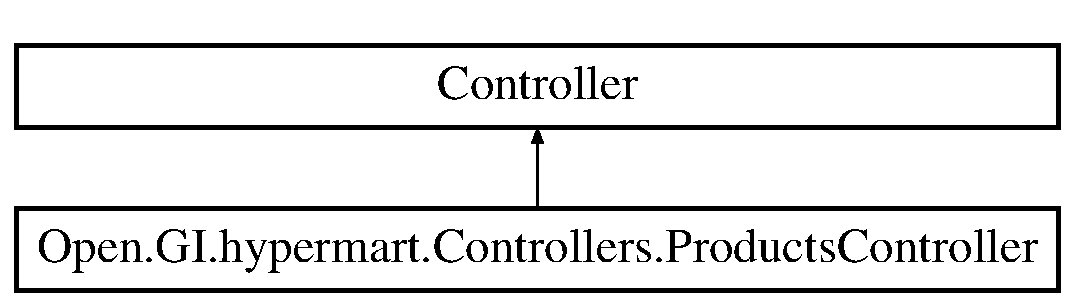
\includegraphics[height=2.000000cm]{class_open_1_1_g_i_1_1hypermart_1_1_controllers_1_1_products_controller}
\end{center}
\end{figure}
\subsection*{Public Member Functions}
\begin{DoxyCompactItemize}
\item 
\textbf{ Products\+Controller} ()
\begin{DoxyCompactList}\small\item\em Initializes a new instance of the \doxyref{Products\+Controller}{p.}{class_open_1_1_g_i_1_1hypermart_1_1_controllers_1_1_products_controller} class. \end{DoxyCompactList}\item 
\textbf{ Products\+Controller} (\textbf{ I\+Hypermart\+Context} \textbf{ db})
\begin{DoxyCompactList}\small\item\em Initializes a new instance of the \doxyref{Products\+Controller}{p.}{class_open_1_1_g_i_1_1hypermart_1_1_controllers_1_1_products_controller} class. \end{DoxyCompactList}\item 
Action\+Result \textbf{ Index} ()
\begin{DoxyCompactList}\small\item\em Indexes this instance. \end{DoxyCompactList}\item 
Action\+Result \textbf{ Details} (int? id)
\begin{DoxyCompactList}\small\item\em Detailses the specified identifier. \end{DoxyCompactList}\item 
Action\+Result \textbf{ Create} ()
\begin{DoxyCompactList}\small\item\em Creates this instance. \end{DoxyCompactList}\item 
Action\+Result \textbf{ Create} ([Bind(Include=\char`\"{}ID,Title,Description,Tagline,Source\+Code,Lead,\char`\"{})] Product product)
\begin{DoxyCompactList}\small\item\em Creates the specified product. \end{DoxyCompactList}\item 
Action\+Result \textbf{ Edit} (int? id)
\begin{DoxyCompactList}\small\item\em Edits the specified identifier. \end{DoxyCompactList}\item 
Action\+Result \textbf{ Edit} ([Bind(Include=\char`\"{}ID,Title,Version,Description,Lead\char`\"{})] Product product)
\begin{DoxyCompactList}\small\item\em Edits the specified product. \end{DoxyCompactList}\item 
Action\+Result \textbf{ Delete} (int? id)
\begin{DoxyCompactList}\small\item\em Deletes the specified identifier. \end{DoxyCompactList}\item 
Action\+Result \textbf{ Delete\+Confirmed} (int id)
\begin{DoxyCompactList}\small\item\em Deletes the confirmed. \end{DoxyCompactList}\end{DoxyCompactItemize}
\subsection*{Protected Member Functions}
\begin{DoxyCompactItemize}
\item 
override void \textbf{ Dispose} (bool disposing)
\begin{DoxyCompactList}\small\item\em Releases unmanaged resources and optionally releases managed resources. \end{DoxyCompactList}\end{DoxyCompactItemize}
\subsection*{Properties}
\begin{DoxyCompactItemize}
\item 
\textbf{ I\+Hypermart\+Context} \textbf{ db}\hspace{0.3cm}{\ttfamily  [get, set]}
\end{DoxyCompactItemize}


\subsection{Detailed Description}


\begin{DoxySeeAlso}{See also}
System.\+Web.\+Mvc.\+Controller


\end{DoxySeeAlso}


Definition at line 19 of file Products\+Controller.\+cs.



\subsection{Constructor \& Destructor Documentation}
\mbox{\label{class_open_1_1_g_i_1_1hypermart_1_1_controllers_1_1_products_controller_aa13f8209001ea23ae8bc01e98eed6326}} 
\index{Open\+::\+G\+I\+::hypermart\+::\+Controllers\+::\+Products\+Controller@{Open\+::\+G\+I\+::hypermart\+::\+Controllers\+::\+Products\+Controller}!Products\+Controller@{Products\+Controller}}
\index{Products\+Controller@{Products\+Controller}!Open\+::\+G\+I\+::hypermart\+::\+Controllers\+::\+Products\+Controller@{Open\+::\+G\+I\+::hypermart\+::\+Controllers\+::\+Products\+Controller}}
\subsubsection{Products\+Controller()\hspace{0.1cm}{\footnotesize\ttfamily [1/2]}}
{\footnotesize\ttfamily Open.\+G\+I.\+hypermart.\+Controllers.\+Products\+Controller.\+Products\+Controller (\begin{DoxyParamCaption}{ }\end{DoxyParamCaption})}



Initializes a new instance of the \doxyref{Products\+Controller}{p.}{class_open_1_1_g_i_1_1hypermart_1_1_controllers_1_1_products_controller} class. 



Definition at line 30 of file Products\+Controller.\+cs.

\mbox{\label{class_open_1_1_g_i_1_1hypermart_1_1_controllers_1_1_products_controller_a6a2c51b106907bf08ce7da150be7424b}} 
\index{Open\+::\+G\+I\+::hypermart\+::\+Controllers\+::\+Products\+Controller@{Open\+::\+G\+I\+::hypermart\+::\+Controllers\+::\+Products\+Controller}!Products\+Controller@{Products\+Controller}}
\index{Products\+Controller@{Products\+Controller}!Open\+::\+G\+I\+::hypermart\+::\+Controllers\+::\+Products\+Controller@{Open\+::\+G\+I\+::hypermart\+::\+Controllers\+::\+Products\+Controller}}
\subsubsection{Products\+Controller()\hspace{0.1cm}{\footnotesize\ttfamily [2/2]}}
{\footnotesize\ttfamily Open.\+G\+I.\+hypermart.\+Controllers.\+Products\+Controller.\+Products\+Controller (\begin{DoxyParamCaption}\item[{\textbf{ I\+Hypermart\+Context}}]{db }\end{DoxyParamCaption})}



Initializes a new instance of the \doxyref{Products\+Controller}{p.}{class_open_1_1_g_i_1_1hypermart_1_1_controllers_1_1_products_controller} class. 


\begin{DoxyParams}{Parameters}
{\em db} & The database.\\
\hline
\end{DoxyParams}


Definition at line 38 of file Products\+Controller.\+cs.



\subsection{Member Function Documentation}
\mbox{\label{class_open_1_1_g_i_1_1hypermart_1_1_controllers_1_1_products_controller_a1ead91e895aa356b20ba2840eafe0a99}} 
\index{Open\+::\+G\+I\+::hypermart\+::\+Controllers\+::\+Products\+Controller@{Open\+::\+G\+I\+::hypermart\+::\+Controllers\+::\+Products\+Controller}!Create@{Create}}
\index{Create@{Create}!Open\+::\+G\+I\+::hypermart\+::\+Controllers\+::\+Products\+Controller@{Open\+::\+G\+I\+::hypermart\+::\+Controllers\+::\+Products\+Controller}}
\subsubsection{Create()\hspace{0.1cm}{\footnotesize\ttfamily [1/2]}}
{\footnotesize\ttfamily Action\+Result Open.\+G\+I.\+hypermart.\+Controllers.\+Products\+Controller.\+Create (\begin{DoxyParamCaption}{ }\end{DoxyParamCaption})}



Creates this instance. 

\begin{DoxyReturn}{Returns}

\end{DoxyReturn}


Definition at line 122 of file Products\+Controller.\+cs.

\mbox{\label{class_open_1_1_g_i_1_1hypermart_1_1_controllers_1_1_products_controller_aa3e20739b645a820cfea38aae81aff6a}} 
\index{Open\+::\+G\+I\+::hypermart\+::\+Controllers\+::\+Products\+Controller@{Open\+::\+G\+I\+::hypermart\+::\+Controllers\+::\+Products\+Controller}!Create@{Create}}
\index{Create@{Create}!Open\+::\+G\+I\+::hypermart\+::\+Controllers\+::\+Products\+Controller@{Open\+::\+G\+I\+::hypermart\+::\+Controllers\+::\+Products\+Controller}}
\subsubsection{Create()\hspace{0.1cm}{\footnotesize\ttfamily [2/2]}}
{\footnotesize\ttfamily Action\+Result Open.\+G\+I.\+hypermart.\+Controllers.\+Products\+Controller.\+Create (\begin{DoxyParamCaption}\item[{[\+Bind(\+Include = \char`\"{}\+I\+D,\+Title,\+Description,\+Tagline,\+Source\+Code,\+Lead,\char`\"{})] \textbf{ Product}}]{product }\end{DoxyParamCaption})}



Creates the specified product. 


\begin{DoxyParams}{Parameters}
{\em product} & The product.\\
\hline
\end{DoxyParams}
\begin{DoxyReturn}{Returns}

\end{DoxyReturn}


Definition at line 137 of file Products\+Controller.\+cs.

\mbox{\label{class_open_1_1_g_i_1_1hypermart_1_1_controllers_1_1_products_controller_a2d8af2d76cdc650951f7f17f66778a62}} 
\index{Open\+::\+G\+I\+::hypermart\+::\+Controllers\+::\+Products\+Controller@{Open\+::\+G\+I\+::hypermart\+::\+Controllers\+::\+Products\+Controller}!Delete@{Delete}}
\index{Delete@{Delete}!Open\+::\+G\+I\+::hypermart\+::\+Controllers\+::\+Products\+Controller@{Open\+::\+G\+I\+::hypermart\+::\+Controllers\+::\+Products\+Controller}}
\subsubsection{Delete()}
{\footnotesize\ttfamily Action\+Result Open.\+G\+I.\+hypermart.\+Controllers.\+Products\+Controller.\+Delete (\begin{DoxyParamCaption}\item[{int?}]{id }\end{DoxyParamCaption})}



Deletes the specified identifier. 


\begin{DoxyParams}{Parameters}
{\em id} & The identifier.\\
\hline
\end{DoxyParams}
\begin{DoxyReturn}{Returns}

\end{DoxyReturn}


Definition at line 227 of file Products\+Controller.\+cs.

\mbox{\label{class_open_1_1_g_i_1_1hypermart_1_1_controllers_1_1_products_controller_a043d74a7640e6cd249143de4c9641404}} 
\index{Open\+::\+G\+I\+::hypermart\+::\+Controllers\+::\+Products\+Controller@{Open\+::\+G\+I\+::hypermart\+::\+Controllers\+::\+Products\+Controller}!Delete\+Confirmed@{Delete\+Confirmed}}
\index{Delete\+Confirmed@{Delete\+Confirmed}!Open\+::\+G\+I\+::hypermart\+::\+Controllers\+::\+Products\+Controller@{Open\+::\+G\+I\+::hypermart\+::\+Controllers\+::\+Products\+Controller}}
\subsubsection{Delete\+Confirmed()}
{\footnotesize\ttfamily Action\+Result Open.\+G\+I.\+hypermart.\+Controllers.\+Products\+Controller.\+Delete\+Confirmed (\begin{DoxyParamCaption}\item[{int}]{id }\end{DoxyParamCaption})}



Deletes the confirmed. 


\begin{DoxyParams}{Parameters}
{\em id} & The identifier.\\
\hline
\end{DoxyParams}
\begin{DoxyReturn}{Returns}

\end{DoxyReturn}


Definition at line 249 of file Products\+Controller.\+cs.

\mbox{\label{class_open_1_1_g_i_1_1hypermart_1_1_controllers_1_1_products_controller_a12f3659f36389715ec436c6a90bc0dc7}} 
\index{Open\+::\+G\+I\+::hypermart\+::\+Controllers\+::\+Products\+Controller@{Open\+::\+G\+I\+::hypermart\+::\+Controllers\+::\+Products\+Controller}!Details@{Details}}
\index{Details@{Details}!Open\+::\+G\+I\+::hypermart\+::\+Controllers\+::\+Products\+Controller@{Open\+::\+G\+I\+::hypermart\+::\+Controllers\+::\+Products\+Controller}}
\subsubsection{Details()}
{\footnotesize\ttfamily Action\+Result Open.\+G\+I.\+hypermart.\+Controllers.\+Products\+Controller.\+Details (\begin{DoxyParamCaption}\item[{int?}]{id }\end{DoxyParamCaption})}



Detailses the specified identifier. 


\begin{DoxyParams}{Parameters}
{\em id} & The identifier.\\
\hline
\end{DoxyParams}
\begin{DoxyReturn}{Returns}

\end{DoxyReturn}


Definition at line 59 of file Products\+Controller.\+cs.

\mbox{\label{class_open_1_1_g_i_1_1hypermart_1_1_controllers_1_1_products_controller_a242db0a0ce58c01d24fc41273dcc393f}} 
\index{Open\+::\+G\+I\+::hypermart\+::\+Controllers\+::\+Products\+Controller@{Open\+::\+G\+I\+::hypermart\+::\+Controllers\+::\+Products\+Controller}!Dispose@{Dispose}}
\index{Dispose@{Dispose}!Open\+::\+G\+I\+::hypermart\+::\+Controllers\+::\+Products\+Controller@{Open\+::\+G\+I\+::hypermart\+::\+Controllers\+::\+Products\+Controller}}
\subsubsection{Dispose()}
{\footnotesize\ttfamily override void Open.\+G\+I.\+hypermart.\+Controllers.\+Products\+Controller.\+Dispose (\begin{DoxyParamCaption}\item[{bool}]{disposing }\end{DoxyParamCaption})\hspace{0.3cm}{\ttfamily [protected]}}



Releases unmanaged resources and optionally releases managed resources. 


\begin{DoxyParams}{Parameters}
{\em disposing} & true to release both managed and unmanaged resources; false to release only unmanaged resources.\\
\hline
\end{DoxyParams}


Definition at line 261 of file Products\+Controller.\+cs.

\mbox{\label{class_open_1_1_g_i_1_1hypermart_1_1_controllers_1_1_products_controller_a203586ae68a295df5c7a037601e4b87a}} 
\index{Open\+::\+G\+I\+::hypermart\+::\+Controllers\+::\+Products\+Controller@{Open\+::\+G\+I\+::hypermart\+::\+Controllers\+::\+Products\+Controller}!Edit@{Edit}}
\index{Edit@{Edit}!Open\+::\+G\+I\+::hypermart\+::\+Controllers\+::\+Products\+Controller@{Open\+::\+G\+I\+::hypermart\+::\+Controllers\+::\+Products\+Controller}}
\subsubsection{Edit()\hspace{0.1cm}{\footnotesize\ttfamily [1/2]}}
{\footnotesize\ttfamily Action\+Result Open.\+G\+I.\+hypermart.\+Controllers.\+Products\+Controller.\+Edit (\begin{DoxyParamCaption}\item[{int?}]{id }\end{DoxyParamCaption})}



Edits the specified identifier. 


\begin{DoxyParams}{Parameters}
{\em id} & The identifier.\\
\hline
\end{DoxyParams}
\begin{DoxyReturn}{Returns}

\end{DoxyReturn}


Definition at line 185 of file Products\+Controller.\+cs.

\mbox{\label{class_open_1_1_g_i_1_1hypermart_1_1_controllers_1_1_products_controller_a7b98181f09525a81fbce5ccb04000546}} 
\index{Open\+::\+G\+I\+::hypermart\+::\+Controllers\+::\+Products\+Controller@{Open\+::\+G\+I\+::hypermart\+::\+Controllers\+::\+Products\+Controller}!Edit@{Edit}}
\index{Edit@{Edit}!Open\+::\+G\+I\+::hypermart\+::\+Controllers\+::\+Products\+Controller@{Open\+::\+G\+I\+::hypermart\+::\+Controllers\+::\+Products\+Controller}}
\subsubsection{Edit()\hspace{0.1cm}{\footnotesize\ttfamily [2/2]}}
{\footnotesize\ttfamily Action\+Result Open.\+G\+I.\+hypermart.\+Controllers.\+Products\+Controller.\+Edit (\begin{DoxyParamCaption}\item[{[\+Bind(\+Include = \char`\"{}\+I\+D,\+Title,\+Version,\+Description,\+Lead\char`\"{})] \textbf{ Product}}]{product }\end{DoxyParamCaption})}



Edits the specified product. 


\begin{DoxyParams}{Parameters}
{\em product} & The product.\\
\hline
\end{DoxyParams}
\begin{DoxyReturn}{Returns}

\end{DoxyReturn}


Definition at line 209 of file Products\+Controller.\+cs.

\mbox{\label{class_open_1_1_g_i_1_1hypermart_1_1_controllers_1_1_products_controller_a244e974803aa1c0f91e8a4fcf0618a9d}} 
\index{Open\+::\+G\+I\+::hypermart\+::\+Controllers\+::\+Products\+Controller@{Open\+::\+G\+I\+::hypermart\+::\+Controllers\+::\+Products\+Controller}!Index@{Index}}
\index{Index@{Index}!Open\+::\+G\+I\+::hypermart\+::\+Controllers\+::\+Products\+Controller@{Open\+::\+G\+I\+::hypermart\+::\+Controllers\+::\+Products\+Controller}}
\subsubsection{Index()}
{\footnotesize\ttfamily Action\+Result Open.\+G\+I.\+hypermart.\+Controllers.\+Products\+Controller.\+Index (\begin{DoxyParamCaption}{ }\end{DoxyParamCaption})}



Indexes this instance. 

\begin{DoxyReturn}{Returns}

\end{DoxyReturn}


Definition at line 48 of file Products\+Controller.\+cs.



\subsection{Property Documentation}
\mbox{\label{class_open_1_1_g_i_1_1hypermart_1_1_controllers_1_1_products_controller_aec73a09108adc7af8384701886c5e53a}} 
\index{Open\+::\+G\+I\+::hypermart\+::\+Controllers\+::\+Products\+Controller@{Open\+::\+G\+I\+::hypermart\+::\+Controllers\+::\+Products\+Controller}!db@{db}}
\index{db@{db}!Open\+::\+G\+I\+::hypermart\+::\+Controllers\+::\+Products\+Controller@{Open\+::\+G\+I\+::hypermart\+::\+Controllers\+::\+Products\+Controller}}
\subsubsection{db}
{\footnotesize\ttfamily \textbf{ I\+Hypermart\+Context} Open.\+G\+I.\+hypermart.\+Controllers.\+Products\+Controller.\+db\hspace{0.3cm}{\ttfamily [get]}, {\ttfamily [set]}}





The database. 

Definition at line 26 of file Products\+Controller.\+cs.



The documentation for this class was generated from the following file\+:\begin{DoxyCompactItemize}
\item 
C\+:/\+Projects/\+App-\/\+Utility-\/\+Store/\+Open.\+G\+I.\+hypermart/\+Controllers/\textbf{ Products\+Controller.\+cs}\end{DoxyCompactItemize}

\hypertarget{class_open_1_1_g_i_1_1hypermart_1_1_models_1_1_rating}{}\section{Open.\+G\+I.\+hypermart.\+Models.\+Rating Class Reference}
\label{class_open_1_1_g_i_1_1hypermart_1_1_models_1_1_rating}\index{Open.\+G\+I.\+hypermart.\+Models.\+Rating@{Open.\+G\+I.\+hypermart.\+Models.\+Rating}}


Model for storing rating information  


\subsection*{Properties}
\begin{DoxyCompactItemize}
\item 
string \hyperlink{class_open_1_1_g_i_1_1hypermart_1_1_models_1_1_rating_a1e8a569cc68356a222db0eee305273f2}{user\+ID}\hspace{0.3cm}{\ttfamily  \mbox{[}get, set\mbox{]}}
\begin{DoxyCompactList}\small\item\em Gets or sets the user identifier. \end{DoxyCompactList}\item 
string \hyperlink{class_open_1_1_g_i_1_1hypermart_1_1_models_1_1_rating_a89b742b6bfd7d9aa0929b73c951fb37e}{Rating\+Category}\hspace{0.3cm}{\ttfamily  \mbox{[}get, set\mbox{]}}
\begin{DoxyCompactList}\small\item\em Gets or sets the rating category. \end{DoxyCompactList}\item 
int \hyperlink{class_open_1_1_g_i_1_1hypermart_1_1_models_1_1_rating_a84ebcfe9c03b3ee3859323be1a9b02da}{Product\+ID}\hspace{0.3cm}{\ttfamily  \mbox{[}get, set\mbox{]}}
\begin{DoxyCompactList}\small\item\em Gets or sets the product identifier. \end{DoxyCompactList}\item 
\hyperlink{class_open_1_1_g_i_1_1hypermart_1_1_models_1_1_product}{Product} \hyperlink{class_open_1_1_g_i_1_1hypermart_1_1_models_1_1_rating_acf0485f546d4d61e33703627040247e8}{Rated\+Product}\hspace{0.3cm}{\ttfamily  \mbox{[}get, set\mbox{]}}
\begin{DoxyCompactList}\small\item\em Gets or sets the rated product. \end{DoxyCompactList}\item 
double \hyperlink{class_open_1_1_g_i_1_1hypermart_1_1_models_1_1_rating_a1090f6d360b3768ba5ad879befb798e0}{rating}\hspace{0.3cm}{\ttfamily  \mbox{[}get, set\mbox{]}}
\begin{DoxyCompactList}\small\item\em Gets or sets the rating. \end{DoxyCompactList}\item 
string \hyperlink{class_open_1_1_g_i_1_1hypermart_1_1_models_1_1_rating_a1b1467d2d1898f6109cc19ec24ee7fd4}{Comments}\hspace{0.3cm}{\ttfamily  \mbox{[}get, set\mbox{]}}
\begin{DoxyCompactList}\small\item\em Gets or sets the comments. \end{DoxyCompactList}\end{DoxyCompactItemize}


\subsection{Detailed Description}
Model for storing rating information 



\subsection{Property Documentation}
\hypertarget{class_open_1_1_g_i_1_1hypermart_1_1_models_1_1_rating_a1b1467d2d1898f6109cc19ec24ee7fd4}{}\label{class_open_1_1_g_i_1_1hypermart_1_1_models_1_1_rating_a1b1467d2d1898f6109cc19ec24ee7fd4} 
\index{Open\+::\+G\+I\+::hypermart\+::\+Models\+::\+Rating@{Open\+::\+G\+I\+::hypermart\+::\+Models\+::\+Rating}!Comments@{Comments}}
\index{Comments@{Comments}!Open\+::\+G\+I\+::hypermart\+::\+Models\+::\+Rating@{Open\+::\+G\+I\+::hypermart\+::\+Models\+::\+Rating}}
\subsubsection{\texorpdfstring{Comments}{Comments}}
{\footnotesize\ttfamily string Open.\+G\+I.\+hypermart.\+Models.\+Rating.\+Comments\hspace{0.3cm}{\ttfamily [get]}, {\ttfamily [set]}}



Gets or sets the comments. 

The comments. \hypertarget{class_open_1_1_g_i_1_1hypermart_1_1_models_1_1_rating_a84ebcfe9c03b3ee3859323be1a9b02da}{}\label{class_open_1_1_g_i_1_1hypermart_1_1_models_1_1_rating_a84ebcfe9c03b3ee3859323be1a9b02da} 
\index{Open\+::\+G\+I\+::hypermart\+::\+Models\+::\+Rating@{Open\+::\+G\+I\+::hypermart\+::\+Models\+::\+Rating}!Product\+ID@{Product\+ID}}
\index{Product\+ID@{Product\+ID}!Open\+::\+G\+I\+::hypermart\+::\+Models\+::\+Rating@{Open\+::\+G\+I\+::hypermart\+::\+Models\+::\+Rating}}
\subsubsection{\texorpdfstring{Product\+ID}{ProductID}}
{\footnotesize\ttfamily int Open.\+G\+I.\+hypermart.\+Models.\+Rating.\+Product\+ID\hspace{0.3cm}{\ttfamily [get]}, {\ttfamily [set]}}



Gets or sets the product identifier. 

The product identifier. \hypertarget{class_open_1_1_g_i_1_1hypermart_1_1_models_1_1_rating_acf0485f546d4d61e33703627040247e8}{}\label{class_open_1_1_g_i_1_1hypermart_1_1_models_1_1_rating_acf0485f546d4d61e33703627040247e8} 
\index{Open\+::\+G\+I\+::hypermart\+::\+Models\+::\+Rating@{Open\+::\+G\+I\+::hypermart\+::\+Models\+::\+Rating}!Rated\+Product@{Rated\+Product}}
\index{Rated\+Product@{Rated\+Product}!Open\+::\+G\+I\+::hypermart\+::\+Models\+::\+Rating@{Open\+::\+G\+I\+::hypermart\+::\+Models\+::\+Rating}}
\subsubsection{\texorpdfstring{Rated\+Product}{RatedProduct}}
{\footnotesize\ttfamily \hyperlink{class_open_1_1_g_i_1_1hypermart_1_1_models_1_1_product}{Product} Open.\+G\+I.\+hypermart.\+Models.\+Rating.\+Rated\+Product\hspace{0.3cm}{\ttfamily [get]}, {\ttfamily [set]}}



Gets or sets the rated product. 

The rated product. \hypertarget{class_open_1_1_g_i_1_1hypermart_1_1_models_1_1_rating_a1090f6d360b3768ba5ad879befb798e0}{}\label{class_open_1_1_g_i_1_1hypermart_1_1_models_1_1_rating_a1090f6d360b3768ba5ad879befb798e0} 
\index{Open\+::\+G\+I\+::hypermart\+::\+Models\+::\+Rating@{Open\+::\+G\+I\+::hypermart\+::\+Models\+::\+Rating}!rating@{rating}}
\index{rating@{rating}!Open\+::\+G\+I\+::hypermart\+::\+Models\+::\+Rating@{Open\+::\+G\+I\+::hypermart\+::\+Models\+::\+Rating}}
\subsubsection{\texorpdfstring{rating}{rating}}
{\footnotesize\ttfamily double Open.\+G\+I.\+hypermart.\+Models.\+Rating.\+rating\hspace{0.3cm}{\ttfamily [get]}, {\ttfamily [set]}}



Gets or sets the rating. 

The rating. \hypertarget{class_open_1_1_g_i_1_1hypermart_1_1_models_1_1_rating_a89b742b6bfd7d9aa0929b73c951fb37e}{}\label{class_open_1_1_g_i_1_1hypermart_1_1_models_1_1_rating_a89b742b6bfd7d9aa0929b73c951fb37e} 
\index{Open\+::\+G\+I\+::hypermart\+::\+Models\+::\+Rating@{Open\+::\+G\+I\+::hypermart\+::\+Models\+::\+Rating}!Rating\+Category@{Rating\+Category}}
\index{Rating\+Category@{Rating\+Category}!Open\+::\+G\+I\+::hypermart\+::\+Models\+::\+Rating@{Open\+::\+G\+I\+::hypermart\+::\+Models\+::\+Rating}}
\subsubsection{\texorpdfstring{Rating\+Category}{RatingCategory}}
{\footnotesize\ttfamily string Open.\+G\+I.\+hypermart.\+Models.\+Rating.\+Rating\+Category\hspace{0.3cm}{\ttfamily [get]}, {\ttfamily [set]}}



Gets or sets the rating category. 

The rating category. \hypertarget{class_open_1_1_g_i_1_1hypermart_1_1_models_1_1_rating_a1e8a569cc68356a222db0eee305273f2}{}\label{class_open_1_1_g_i_1_1hypermart_1_1_models_1_1_rating_a1e8a569cc68356a222db0eee305273f2} 
\index{Open\+::\+G\+I\+::hypermart\+::\+Models\+::\+Rating@{Open\+::\+G\+I\+::hypermart\+::\+Models\+::\+Rating}!user\+ID@{user\+ID}}
\index{user\+ID@{user\+ID}!Open\+::\+G\+I\+::hypermart\+::\+Models\+::\+Rating@{Open\+::\+G\+I\+::hypermart\+::\+Models\+::\+Rating}}
\subsubsection{\texorpdfstring{user\+ID}{userID}}
{\footnotesize\ttfamily string Open.\+G\+I.\+hypermart.\+Models.\+Rating.\+user\+ID\hspace{0.3cm}{\ttfamily [get]}, {\ttfamily [set]}}



Gets or sets the user identifier. 

The user identifier. 

The documentation for this class was generated from the following file\+:\begin{DoxyCompactItemize}
\item 
C\+:/\+Projects/\+App-\/\+Utility-\/\+Store/\+Open.\+G\+I.\+hypermart/\+Models/\hyperlink{_rating_8cs}{Rating.\+cs}\end{DoxyCompactItemize}

\hypertarget{class_open_1_1_g_i_1_1hypermart_1_1_route_config}{}\section{Open.\+G\+I.\+hypermart.\+Route\+Config Class Reference}
\label{class_open_1_1_g_i_1_1hypermart_1_1_route_config}\index{Open.\+G\+I.\+hypermart.\+Route\+Config@{Open.\+G\+I.\+hypermart.\+Route\+Config}}


M\+V\+C -\/ Route Registration  


\subsection*{Static Public Member Functions}
\begin{DoxyCompactItemize}
\item 
static void \hyperlink{class_open_1_1_g_i_1_1hypermart_1_1_route_config_a9b4bb82c10a972d509a88ad37cb1c783}{Register\+Routes} (Route\+Collection routes)
\begin{DoxyCompactList}\small\item\em Registers the routes. \end{DoxyCompactList}\end{DoxyCompactItemize}


\subsection{Detailed Description}
M\+V\+C -\/ Route Registration 



Definition at line 13 of file Route\+Config.\+cs.



\subsection{Member Function Documentation}
\hypertarget{class_open_1_1_g_i_1_1hypermart_1_1_route_config_a9b4bb82c10a972d509a88ad37cb1c783}{}\index{Open\+::\+G\+I\+::hypermart\+::\+Route\+Config@{Open\+::\+G\+I\+::hypermart\+::\+Route\+Config}!Register\+Routes@{Register\+Routes}}
\index{Register\+Routes@{Register\+Routes}!Open\+::\+G\+I\+::hypermart\+::\+Route\+Config@{Open\+::\+G\+I\+::hypermart\+::\+Route\+Config}}
\subsubsection[{Register\+Routes(\+Route\+Collection routes)}]{\setlength{\rightskip}{0pt plus 5cm}static void Open.\+G\+I.\+hypermart.\+Route\+Config.\+Register\+Routes (
\begin{DoxyParamCaption}
\item[{Route\+Collection}]{routes}
\end{DoxyParamCaption}
)\hspace{0.3cm}{\ttfamily [static]}}\label{class_open_1_1_g_i_1_1hypermart_1_1_route_config_a9b4bb82c10a972d509a88ad37cb1c783}


Registers the routes. 


\begin{DoxyParams}{Parameters}
{\em routes} & The routes.\\
\hline
\end{DoxyParams}


Definition at line 19 of file Route\+Config.\+cs.



The documentation for this class was generated from the following file\+:\begin{DoxyCompactItemize}
\item 
C\+:/\+Projects/\+App-\/\+Utility-\/\+Store/\+Open.\+G\+I.\+hypermart/\+App\+\_\+\+Start/\hyperlink{_route_config_8cs}{Route\+Config.\+cs}\end{DoxyCompactItemize}

\hypertarget{class_open_1_1_g_i_1_1hypermart_1_1_helpers_1_1_rss_action_result}{}\section{Open.\+G\+I.\+hypermart.\+Helpers.\+Rss\+Action\+Result Class Reference}
\label{class_open_1_1_g_i_1_1hypermart_1_1_helpers_1_1_rss_action_result}\index{Open.\+G\+I.\+hypermart.\+Helpers.\+Rss\+Action\+Result@{Open.\+G\+I.\+hypermart.\+Helpers.\+Rss\+Action\+Result}}


R\+SS Action Results  


Inheritance diagram for Open.\+G\+I.\+hypermart.\+Helpers.\+Rss\+Action\+Result\+:\begin{figure}[H]
\begin{center}
\leavevmode
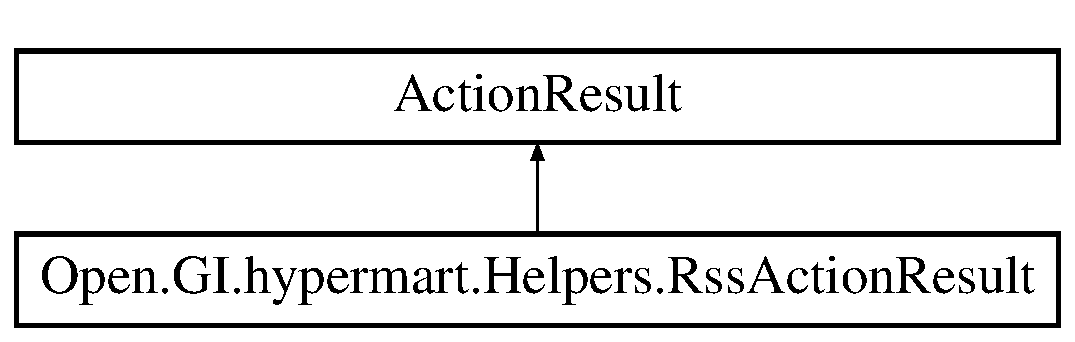
\includegraphics[height=2.000000cm]{class_open_1_1_g_i_1_1hypermart_1_1_helpers_1_1_rss_action_result}
\end{center}
\end{figure}
\subsection*{Public Member Functions}
\begin{DoxyCompactItemize}
\item 
override void \hyperlink{class_open_1_1_g_i_1_1hypermart_1_1_helpers_1_1_rss_action_result_a18ff30f679b2858b2d88a7dc267fd672}{Execute\+Result} (Controller\+Context context)
\begin{DoxyCompactList}\small\item\em Enables processing of the result of an action method by a custom type that inherits from the T\+:\+System.\+Web.\+Mvc.\+Action\+Result class. \end{DoxyCompactList}\end{DoxyCompactItemize}
\subsection*{Properties}
\begin{DoxyCompactItemize}
\item 
Syndication\+Feed \hyperlink{class_open_1_1_g_i_1_1hypermart_1_1_helpers_1_1_rss_action_result_a3b07cc4558b6a4863821fbedd9aa6888}{Feed}\hspace{0.3cm}{\ttfamily  \mbox{[}get, set\mbox{]}}
\begin{DoxyCompactList}\small\item\em Gets or sets the feed. \end{DoxyCompactList}\end{DoxyCompactItemize}


\subsection{Detailed Description}
R\+SS Action Results 

\begin{DoxySeeAlso}{See also}
System.\+Web.\+Mvc.\+Action\+Result


\end{DoxySeeAlso}


\subsection{Member Function Documentation}
\hypertarget{class_open_1_1_g_i_1_1hypermart_1_1_helpers_1_1_rss_action_result_a18ff30f679b2858b2d88a7dc267fd672}{}\label{class_open_1_1_g_i_1_1hypermart_1_1_helpers_1_1_rss_action_result_a18ff30f679b2858b2d88a7dc267fd672} 
\index{Open\+::\+G\+I\+::hypermart\+::\+Helpers\+::\+Rss\+Action\+Result@{Open\+::\+G\+I\+::hypermart\+::\+Helpers\+::\+Rss\+Action\+Result}!Execute\+Result@{Execute\+Result}}
\index{Execute\+Result@{Execute\+Result}!Open\+::\+G\+I\+::hypermart\+::\+Helpers\+::\+Rss\+Action\+Result@{Open\+::\+G\+I\+::hypermart\+::\+Helpers\+::\+Rss\+Action\+Result}}
\subsubsection{\texorpdfstring{Execute\+Result()}{ExecuteResult()}}
{\footnotesize\ttfamily override void Open.\+G\+I.\+hypermart.\+Helpers.\+Rss\+Action\+Result.\+Execute\+Result (\begin{DoxyParamCaption}\item[{Controller\+Context}]{context }\end{DoxyParamCaption})}



Enables processing of the result of an action method by a custom type that inherits from the T\+:\+System.\+Web.\+Mvc.\+Action\+Result class. 


\begin{DoxyParams}{Parameters}
{\em context} & The context in which the result is executed. The context information includes the controller, H\+T\+TP content, request context, and route data.\\
\hline
\end{DoxyParams}


\subsection{Property Documentation}
\hypertarget{class_open_1_1_g_i_1_1hypermart_1_1_helpers_1_1_rss_action_result_a3b07cc4558b6a4863821fbedd9aa6888}{}\label{class_open_1_1_g_i_1_1hypermart_1_1_helpers_1_1_rss_action_result_a3b07cc4558b6a4863821fbedd9aa6888} 
\index{Open\+::\+G\+I\+::hypermart\+::\+Helpers\+::\+Rss\+Action\+Result@{Open\+::\+G\+I\+::hypermart\+::\+Helpers\+::\+Rss\+Action\+Result}!Feed@{Feed}}
\index{Feed@{Feed}!Open\+::\+G\+I\+::hypermart\+::\+Helpers\+::\+Rss\+Action\+Result@{Open\+::\+G\+I\+::hypermart\+::\+Helpers\+::\+Rss\+Action\+Result}}
\subsubsection{\texorpdfstring{Feed}{Feed}}
{\footnotesize\ttfamily Syndication\+Feed Open.\+G\+I.\+hypermart.\+Helpers.\+Rss\+Action\+Result.\+Feed\hspace{0.3cm}{\ttfamily [get]}, {\ttfamily [set]}}



Gets or sets the feed. 

The feed. 

The documentation for this class was generated from the following file\+:\begin{DoxyCompactItemize}
\item 
C\+:/\+Projects/\+App-\/\+Utility-\/\+Store/\+Open.\+G\+I.\+hypermart/\+Helpers/\hyperlink{_rss_action_result_8cs}{Rss\+Action\+Result.\+cs}\end{DoxyCompactItemize}

\section{Open.\+G\+I.\+hypermart.\+Models.\+Screenshot Class Reference}
\label{class_open_1_1_g_i_1_1hypermart_1_1_models_1_1_screenshot}\index{Open.\+G\+I.\+hypermart.\+Models.\+Screenshot@{Open.\+G\+I.\+hypermart.\+Models.\+Screenshot}}


Screen Shot Model Class  


\subsection*{Properties}
\begin{DoxyCompactItemize}
\item 
int \textbf{ ID}\hspace{0.3cm}{\ttfamily  [get, set]}
\begin{DoxyCompactList}\small\item\em Gets or sets the identifier. \end{DoxyCompactList}\item 
byte [$\,$] \textbf{ Screen\+Shot1}\hspace{0.3cm}{\ttfamily  [get, set]}
\begin{DoxyCompactList}\small\item\em Gets or sets the screen shot1. \end{DoxyCompactList}\item 
int \textbf{ Product\+ID}\hspace{0.3cm}{\ttfamily  [get, set]}
\begin{DoxyCompactList}\small\item\em Gets or sets the product\+\_\+ identifier. \end{DoxyCompactList}\item 
\textbf{ Product} \textbf{ Product}\hspace{0.3cm}{\ttfamily  [get, set]}
\begin{DoxyCompactList}\small\item\em Gets or sets the product. \end{DoxyCompactList}\item 
virtual \textbf{ Product} \textbf{ Product}\hspace{0.3cm}{\ttfamily  [get, set]}
\end{DoxyCompactItemize}


\subsection{Detailed Description}
Screen Shot Model Class 



Definition at line 12 of file Screenshot.\+cs.



\subsection{Property Documentation}
\mbox{\label{class_open_1_1_g_i_1_1hypermart_1_1_models_1_1_screenshot_a7460fabffe75a362966595c8b86cdef2}} 
\index{Open\+::\+G\+I\+::hypermart\+::\+Models\+::\+Screenshot@{Open\+::\+G\+I\+::hypermart\+::\+Models\+::\+Screenshot}!ID@{ID}}
\index{ID@{ID}!Open\+::\+G\+I\+::hypermart\+::\+Models\+::\+Screenshot@{Open\+::\+G\+I\+::hypermart\+::\+Models\+::\+Screenshot}}
\subsubsection{ID}
{\footnotesize\ttfamily int Open.\+G\+I.\+hypermart.\+Models.\+Screenshot.\+ID\hspace{0.3cm}{\ttfamily [get]}, {\ttfamily [set]}}



Gets or sets the identifier. 

The identifier. 

Definition at line 20 of file Screenshot.\+cs.

\mbox{\label{class_open_1_1_g_i_1_1hypermart_1_1_models_1_1_screenshot_a8aed1d2289db7caefe8c7e14e0f5cc50}} 
\index{Open\+::\+G\+I\+::hypermart\+::\+Models\+::\+Screenshot@{Open\+::\+G\+I\+::hypermart\+::\+Models\+::\+Screenshot}!Product@{Product}}
\index{Product@{Product}!Open\+::\+G\+I\+::hypermart\+::\+Models\+::\+Screenshot@{Open\+::\+G\+I\+::hypermart\+::\+Models\+::\+Screenshot}}
\subsubsection{Product\hspace{0.1cm}{\footnotesize\ttfamily [1/2]}}
{\footnotesize\ttfamily virtual \textbf{ Product} Open.\+G\+I.\+hypermart.\+Models.\+Screenshot.\+Product\hspace{0.3cm}{\ttfamily [get]}, {\ttfamily [set]}}



Definition at line 21 of file Screenshot.\+cs.

\mbox{\label{class_open_1_1_g_i_1_1hypermart_1_1_models_1_1_screenshot_ae4e4b60e07136a6c4debe888426d6f6b}} 
\index{Open\+::\+G\+I\+::hypermart\+::\+Models\+::\+Screenshot@{Open\+::\+G\+I\+::hypermart\+::\+Models\+::\+Screenshot}!Product@{Product}}
\index{Product@{Product}!Open\+::\+G\+I\+::hypermart\+::\+Models\+::\+Screenshot@{Open\+::\+G\+I\+::hypermart\+::\+Models\+::\+Screenshot}}
\subsubsection{Product\hspace{0.1cm}{\footnotesize\ttfamily [2/2]}}
{\footnotesize\ttfamily \textbf{ Product} Open.\+G\+I.\+hypermart.\+Models.\+Screenshot.\+Product\hspace{0.3cm}{\ttfamily [get]}, {\ttfamily [set]}}



Gets or sets the product. 

The product. 

Definition at line 46 of file Screenshot.\+cs.

\mbox{\label{class_open_1_1_g_i_1_1hypermart_1_1_models_1_1_screenshot_ad381abf51bb0ebb1c2566c70df11c05a}} 
\index{Open\+::\+G\+I\+::hypermart\+::\+Models\+::\+Screenshot@{Open\+::\+G\+I\+::hypermart\+::\+Models\+::\+Screenshot}!Product\+ID@{Product\+ID}}
\index{Product\+ID@{Product\+ID}!Open\+::\+G\+I\+::hypermart\+::\+Models\+::\+Screenshot@{Open\+::\+G\+I\+::hypermart\+::\+Models\+::\+Screenshot}}
\subsubsection{Product\+ID}
{\footnotesize\ttfamily int Open.\+G\+I.\+hypermart.\+Models.\+Screenshot.\+Product\+ID\hspace{0.3cm}{\ttfamily [get]}, {\ttfamily [set]}}



Gets or sets the product\+\_\+ identifier. 

The product\+\_\+ identifier. 

Definition at line 38 of file Screenshot.\+cs.

\mbox{\label{class_open_1_1_g_i_1_1hypermart_1_1_models_1_1_screenshot_a435ca1863d66de2de497d603585610d8}} 
\index{Open\+::\+G\+I\+::hypermart\+::\+Models\+::\+Screenshot@{Open\+::\+G\+I\+::hypermart\+::\+Models\+::\+Screenshot}!Screen\+Shot1@{Screen\+Shot1}}
\index{Screen\+Shot1@{Screen\+Shot1}!Open\+::\+G\+I\+::hypermart\+::\+Models\+::\+Screenshot@{Open\+::\+G\+I\+::hypermart\+::\+Models\+::\+Screenshot}}
\subsubsection{Screen\+Shot1}
{\footnotesize\ttfamily byte [$\,$] Open.\+G\+I.\+hypermart.\+Models.\+Screenshot.\+Screen\+Shot1\hspace{0.3cm}{\ttfamily [get]}, {\ttfamily [set]}}



Gets or sets the screen shot1. 

The screen shot1. 

Definition at line 30 of file Screenshot.\+cs.



The documentation for this class was generated from the following file\+:\begin{DoxyCompactItemize}
\item 
C\+:/\+Projects/\+App-\/\+Utility-\/\+Store/\+Open.\+G\+I.\+hypermart/\+Models/\textbf{ Screenshot.\+cs}\end{DoxyCompactItemize}

\hypertarget{class_open_1_1_g_i_1_1hypermart_1_1_areas_1_1_help_page_1_1_model_descriptions_1_1_simple_type_model_description}{}\section{Open.\+G\+I.\+hypermart.\+Areas.\+Help\+Page.\+Model\+Descriptions.\+Simple\+Type\+Model\+Description Class Reference}
\label{class_open_1_1_g_i_1_1hypermart_1_1_areas_1_1_help_page_1_1_model_descriptions_1_1_simple_type_model_description}\index{Open.\+G\+I.\+hypermart.\+Areas.\+Help\+Page.\+Model\+Descriptions.\+Simple\+Type\+Model\+Description@{Open.\+G\+I.\+hypermart.\+Areas.\+Help\+Page.\+Model\+Descriptions.\+Simple\+Type\+Model\+Description}}


 


Inheritance diagram for Open.\+G\+I.\+hypermart.\+Areas.\+Help\+Page.\+Model\+Descriptions.\+Simple\+Type\+Model\+Description\+:\begin{figure}[H]
\begin{center}
\leavevmode
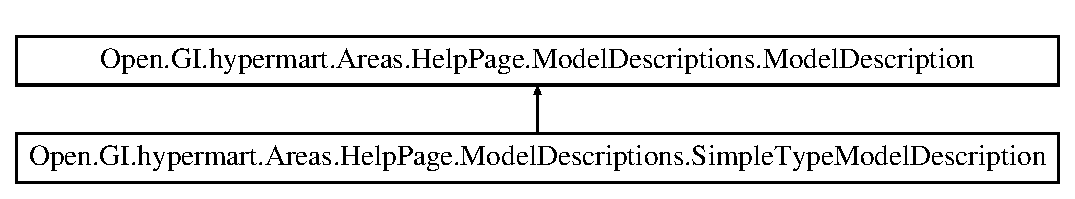
\includegraphics[height=2.000000cm]{class_open_1_1_g_i_1_1hypermart_1_1_areas_1_1_help_page_1_1_model_descriptions_1_1_simple_type_model_description}
\end{center}
\end{figure}
\subsection*{Additional Inherited Members}


\subsection{Detailed Description}


\begin{DoxySeeAlso}{See also}
\hyperlink{class_open_1_1_g_i_1_1hypermart_1_1_areas_1_1_help_page_1_1_model_descriptions_1_1_model_description}{Open.\+G\+I.\+hypermart.\+Areas.\+Help\+Page.\+Model\+Descriptions.\+Model\+Description}


\end{DoxySeeAlso}


Definition at line 7 of file Simple\+Type\+Model\+Description.\+cs.



The documentation for this class was generated from the following file\+:\begin{DoxyCompactItemize}
\item 
C\+:/\+Projects/\+App-\/\+Utility-\/\+Store/\+Open.\+G\+I.\+hypermart/\+Areas/\+Help\+Page/\+Model\+Descriptions/\hyperlink{_simple_type_model_description_8cs}{Simple\+Type\+Model\+Description.\+cs}\end{DoxyCompactItemize}

\section{Open.\+G\+I.\+hypermart.\+Status Class Reference}
\label{class_open_1_1_g_i_1_1hypermart_1_1_status}\index{Open.\+G\+I.\+hypermart.\+Status@{Open.\+G\+I.\+hypermart.\+Status}}


Summary description for \doxyref{Status}{p.}{class_open_1_1_g_i_1_1hypermart_1_1_status}  


Inheritance diagram for Open.\+G\+I.\+hypermart.\+Status\+:\begin{figure}[H]
\begin{center}
\leavevmode
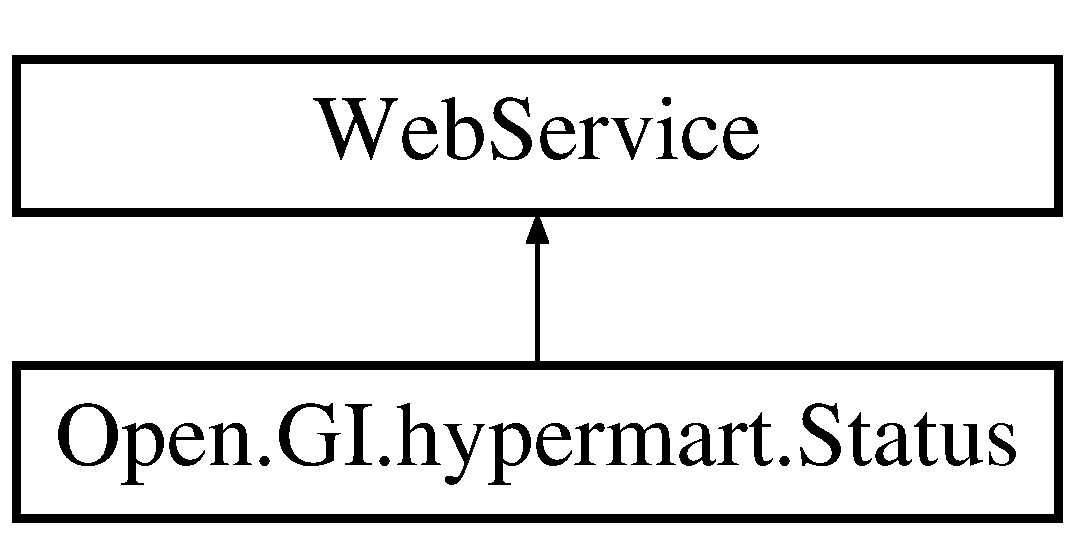
\includegraphics[height=2.000000cm]{class_open_1_1_g_i_1_1hypermart_1_1_status}
\end{center}
\end{figure}
\subsection*{Public Member Functions}
\begin{DoxyCompactItemize}
\item 
string \textbf{ Hello\+World} ()
\begin{DoxyCompactList}\small\item\em This is the Hello World method. \end{DoxyCompactList}\end{DoxyCompactItemize}


\subsection{Detailed Description}
Summary description for \doxyref{Status}{p.}{class_open_1_1_g_i_1_1hypermart_1_1_status} 



Definition at line 17 of file Status.\+asmx.\+cs.



\subsection{Member Function Documentation}
\mbox{\label{class_open_1_1_g_i_1_1hypermart_1_1_status_a73a11d6869226091bd66017995dfabef}} 
\index{Open\+::\+G\+I\+::hypermart\+::\+Status@{Open\+::\+G\+I\+::hypermart\+::\+Status}!Hello\+World@{Hello\+World}}
\index{Hello\+World@{Hello\+World}!Open\+::\+G\+I\+::hypermart\+::\+Status@{Open\+::\+G\+I\+::hypermart\+::\+Status}}
\subsubsection{Hello\+World()}
{\footnotesize\ttfamily string Open.\+G\+I.\+hypermart.\+Status.\+Hello\+World (\begin{DoxyParamCaption}{ }\end{DoxyParamCaption})}



This is the Hello World method. 

\begin{DoxyReturn}{Returns}

\end{DoxyReturn}


Definition at line 25 of file Status.\+asmx.\+cs.



The documentation for this class was generated from the following file\+:\begin{DoxyCompactItemize}
\item 
C\+:/\+Projects/\+App-\/\+Utility-\/\+Store/\+Open.\+G\+I.\+hypermart/\textbf{ Status.\+asmx.\+cs}\end{DoxyCompactItemize}

\section{Open.\+G\+I.\+hypermart.\+Controllers.\+Store\+Content\+Controller Class Reference}
\label{class_open_1_1_g_i_1_1hypermart_1_1_controllers_1_1_store_content_controller}\index{Open.\+G\+I.\+hypermart.\+Controllers.\+Store\+Content\+Controller@{Open.\+G\+I.\+hypermart.\+Controllers.\+Store\+Content\+Controller}}


This is the Open\+GI \doxyref{A\+PI}{p.}{namespace_open_1_1_g_i_1_1hypermart_1_1_controllers_1_1_a_p_i} layer for interacting with the Store(\+Ading content etc). Some of the calls here relating to updates and creation will require a session token.  


Inheritance diagram for Open.\+G\+I.\+hypermart.\+Controllers.\+Store\+Content\+Controller\+:\begin{figure}[H]
\begin{center}
\leavevmode
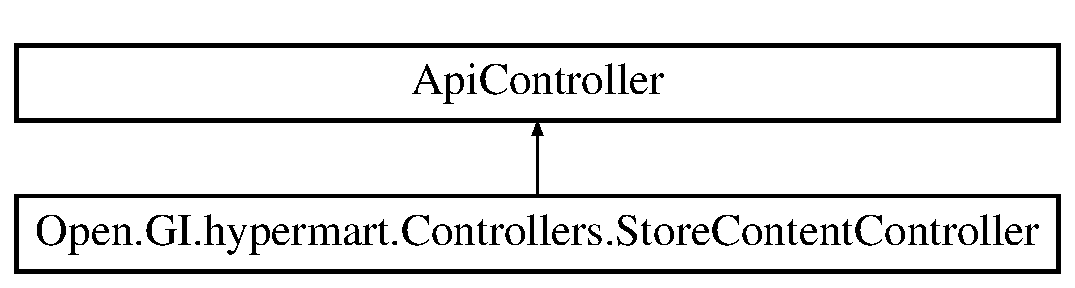
\includegraphics[height=2.000000cm]{class_open_1_1_g_i_1_1hypermart_1_1_controllers_1_1_store_content_controller}
\end{center}
\end{figure}
\subsection*{Public Member Functions}
\begin{DoxyCompactItemize}
\item 
\textbf{ Store\+Content\+Controller} ()
\begin{DoxyCompactList}\small\item\em Initializes a new instance of the \doxyref{Store\+Content\+Controller}{p.}{class_open_1_1_g_i_1_1hypermart_1_1_controllers_1_1_store_content_controller} class. \end{DoxyCompactList}\item 
\textbf{ Store\+Content\+Controller} (\textbf{ I\+Hypermart\+Context} db\+Context)
\begin{DoxyCompactList}\small\item\em Initializes a new instance of the \doxyref{Store\+Content\+Controller}{p.}{class_open_1_1_g_i_1_1hypermart_1_1_controllers_1_1_store_content_controller} class. \end{DoxyCompactList}\item 
I\+Queryable$<$ \textbf{ Product\+D\+TO} $>$ \textbf{ Get\+All\+Products} ()
\begin{DoxyCompactList}\small\item\em Gets all products. \end{DoxyCompactList}\item 
\textbf{ Product\+D\+TO} \textbf{ Get\+Product} (int id)
\begin{DoxyCompactList}\small\item\em Gets a product. \end{DoxyCompactList}\item 
\textbf{ Product\+D\+TO} \textbf{ Post\+Product} (\textbf{ Product} item\+To\+Add)
\begin{DoxyCompactList}\small\item\em Create a New Product \end{DoxyCompactList}\item 
bool \textbf{ Delete\+Product} (\textbf{ Product} product\+To\+Delete)
\begin{DoxyCompactList}\small\item\em Deletes the product. \end{DoxyCompactList}\item 
void \textbf{ Delete\+Product} (int Product\+ID)
\begin{DoxyCompactList}\small\item\em Deletes the product. \end{DoxyCompactList}\item 
List$<$ \textbf{ File\+D\+TO} $>$ \textbf{ Get\+Files} (int id)
\begin{DoxyCompactList}\small\item\em Gets all files for a product. \end{DoxyCompactList}\item 
\textbf{ File\+D\+TO} \textbf{ Post\+Product\+File} (int Product\+ID, \textbf{ Open.\+G\+I.\+hypermart.\+Models.\+File} File\+To\+Add)
\begin{DoxyCompactList}\small\item\em Posts the product file. \end{DoxyCompactList}\item 
\textbf{ File\+D\+TO} \textbf{ Add\+File} (int Product\+ID, \textbf{ Open.\+G\+I.\+hypermart.\+Models.\+File} File\+To\+Add)
\begin{DoxyCompactList}\small\item\em Add A File to a product \end{DoxyCompactList}\item 
void \textbf{ Add\+Screen\+Shot} (int Product\+ID)
\begin{DoxyCompactList}\small\item\em Add a Screenshot to an Product \end{DoxyCompactList}\item 
void \textbf{ Post\+Ratings} (\textbf{ Rating\+Information\+D\+TO} Rating\+To\+Add)
\begin{DoxyCompactList}\small\item\em Create a New Product Rating \end{DoxyCompactList}\end{DoxyCompactItemize}


\subsection{Detailed Description}
This is the Open\+GI \doxyref{A\+PI}{p.}{namespace_open_1_1_g_i_1_1hypermart_1_1_controllers_1_1_a_p_i} layer for interacting with the Store(\+Ading content etc). Some of the calls here relating to updates and creation will require a session token. 



Definition at line 21 of file Store\+Content\+Controller.\+cs.



\subsection{Constructor \& Destructor Documentation}
\mbox{\label{class_open_1_1_g_i_1_1hypermart_1_1_controllers_1_1_store_content_controller_a01bad24ca04f869ec58d136ff35b2d13}} 
\index{Open\+::\+G\+I\+::hypermart\+::\+Controllers\+::\+Store\+Content\+Controller@{Open\+::\+G\+I\+::hypermart\+::\+Controllers\+::\+Store\+Content\+Controller}!Store\+Content\+Controller@{Store\+Content\+Controller}}
\index{Store\+Content\+Controller@{Store\+Content\+Controller}!Open\+::\+G\+I\+::hypermart\+::\+Controllers\+::\+Store\+Content\+Controller@{Open\+::\+G\+I\+::hypermart\+::\+Controllers\+::\+Store\+Content\+Controller}}
\subsubsection{Store\+Content\+Controller()\hspace{0.1cm}{\footnotesize\ttfamily [1/2]}}
{\footnotesize\ttfamily Open.\+G\+I.\+hypermart.\+Controllers.\+Store\+Content\+Controller.\+Store\+Content\+Controller (\begin{DoxyParamCaption}{ }\end{DoxyParamCaption})}



Initializes a new instance of the \doxyref{Store\+Content\+Controller}{p.}{class_open_1_1_g_i_1_1hypermart_1_1_controllers_1_1_store_content_controller} class. 



Definition at line 27 of file Store\+Content\+Controller.\+cs.

\mbox{\label{class_open_1_1_g_i_1_1hypermart_1_1_controllers_1_1_store_content_controller_ad8b3b3f13892bbb028eb21b7e240d7e2}} 
\index{Open\+::\+G\+I\+::hypermart\+::\+Controllers\+::\+Store\+Content\+Controller@{Open\+::\+G\+I\+::hypermart\+::\+Controllers\+::\+Store\+Content\+Controller}!Store\+Content\+Controller@{Store\+Content\+Controller}}
\index{Store\+Content\+Controller@{Store\+Content\+Controller}!Open\+::\+G\+I\+::hypermart\+::\+Controllers\+::\+Store\+Content\+Controller@{Open\+::\+G\+I\+::hypermart\+::\+Controllers\+::\+Store\+Content\+Controller}}
\subsubsection{Store\+Content\+Controller()\hspace{0.1cm}{\footnotesize\ttfamily [2/2]}}
{\footnotesize\ttfamily Open.\+G\+I.\+hypermart.\+Controllers.\+Store\+Content\+Controller.\+Store\+Content\+Controller (\begin{DoxyParamCaption}\item[{\textbf{ I\+Hypermart\+Context}}]{db\+Context }\end{DoxyParamCaption})}



Initializes a new instance of the \doxyref{Store\+Content\+Controller}{p.}{class_open_1_1_g_i_1_1hypermart_1_1_controllers_1_1_store_content_controller} class. 


\begin{DoxyParams}{Parameters}
{\em db\+Context} & The database context.\\
\hline
\end{DoxyParams}


Definition at line 36 of file Store\+Content\+Controller.\+cs.



\subsection{Member Function Documentation}
\mbox{\label{class_open_1_1_g_i_1_1hypermart_1_1_controllers_1_1_store_content_controller_a36a438b2ab2cbb1d937b6a4c5bd8b17d}} 
\index{Open\+::\+G\+I\+::hypermart\+::\+Controllers\+::\+Store\+Content\+Controller@{Open\+::\+G\+I\+::hypermart\+::\+Controllers\+::\+Store\+Content\+Controller}!Add\+File@{Add\+File}}
\index{Add\+File@{Add\+File}!Open\+::\+G\+I\+::hypermart\+::\+Controllers\+::\+Store\+Content\+Controller@{Open\+::\+G\+I\+::hypermart\+::\+Controllers\+::\+Store\+Content\+Controller}}
\subsubsection{Add\+File()}
{\footnotesize\ttfamily \textbf{ File\+D\+TO} Open.\+G\+I.\+hypermart.\+Controllers.\+Store\+Content\+Controller.\+Add\+File (\begin{DoxyParamCaption}\item[{int}]{Product\+ID,  }\item[{\textbf{ Open.\+G\+I.\+hypermart.\+Models.\+File}}]{File\+To\+Add }\end{DoxyParamCaption})}



Add A File to a product 


\begin{DoxyParams}{Parameters}
{\em Product\+ID} & \\
\hline
{\em File\+To\+Add} & \\
\hline
\end{DoxyParams}
\begin{DoxyReturn}{Returns}

\end{DoxyReturn}


Definition at line 211 of file Store\+Content\+Controller.\+cs.

\mbox{\label{class_open_1_1_g_i_1_1hypermart_1_1_controllers_1_1_store_content_controller_a7c5b861d456ae7b592165634a07c6738}} 
\index{Open\+::\+G\+I\+::hypermart\+::\+Controllers\+::\+Store\+Content\+Controller@{Open\+::\+G\+I\+::hypermart\+::\+Controllers\+::\+Store\+Content\+Controller}!Add\+Screen\+Shot@{Add\+Screen\+Shot}}
\index{Add\+Screen\+Shot@{Add\+Screen\+Shot}!Open\+::\+G\+I\+::hypermart\+::\+Controllers\+::\+Store\+Content\+Controller@{Open\+::\+G\+I\+::hypermart\+::\+Controllers\+::\+Store\+Content\+Controller}}
\subsubsection{Add\+Screen\+Shot()}
{\footnotesize\ttfamily void Open.\+G\+I.\+hypermart.\+Controllers.\+Store\+Content\+Controller.\+Add\+Screen\+Shot (\begin{DoxyParamCaption}\item[{int}]{Product\+ID }\end{DoxyParamCaption})}



Add a Screenshot to an Product 


\begin{DoxyParams}{Parameters}
{\em Product\+ID} & \\
\hline
\end{DoxyParams}


Definition at line 236 of file Store\+Content\+Controller.\+cs.

\mbox{\label{class_open_1_1_g_i_1_1hypermart_1_1_controllers_1_1_store_content_controller_a3e98139b9c8d95c6afb1bbe699aff201}} 
\index{Open\+::\+G\+I\+::hypermart\+::\+Controllers\+::\+Store\+Content\+Controller@{Open\+::\+G\+I\+::hypermart\+::\+Controllers\+::\+Store\+Content\+Controller}!Delete\+Product@{Delete\+Product}}
\index{Delete\+Product@{Delete\+Product}!Open\+::\+G\+I\+::hypermart\+::\+Controllers\+::\+Store\+Content\+Controller@{Open\+::\+G\+I\+::hypermart\+::\+Controllers\+::\+Store\+Content\+Controller}}
\subsubsection{Delete\+Product()\hspace{0.1cm}{\footnotesize\ttfamily [1/2]}}
{\footnotesize\ttfamily bool Open.\+G\+I.\+hypermart.\+Controllers.\+Store\+Content\+Controller.\+Delete\+Product (\begin{DoxyParamCaption}\item[{\textbf{ Product}}]{product\+To\+Delete }\end{DoxyParamCaption})}



Deletes the product. 


\begin{DoxyParams}{Parameters}
{\em product\+To\+Delete} & The product to delete.\\
\hline
\end{DoxyParams}
\begin{DoxyReturn}{Returns}

\end{DoxyReturn}


Definition at line 126 of file Store\+Content\+Controller.\+cs.

\mbox{\label{class_open_1_1_g_i_1_1hypermart_1_1_controllers_1_1_store_content_controller_aee0d4040607c0d07828fc0d000135fcd}} 
\index{Open\+::\+G\+I\+::hypermart\+::\+Controllers\+::\+Store\+Content\+Controller@{Open\+::\+G\+I\+::hypermart\+::\+Controllers\+::\+Store\+Content\+Controller}!Delete\+Product@{Delete\+Product}}
\index{Delete\+Product@{Delete\+Product}!Open\+::\+G\+I\+::hypermart\+::\+Controllers\+::\+Store\+Content\+Controller@{Open\+::\+G\+I\+::hypermart\+::\+Controllers\+::\+Store\+Content\+Controller}}
\subsubsection{Delete\+Product()\hspace{0.1cm}{\footnotesize\ttfamily [2/2]}}
{\footnotesize\ttfamily void Open.\+G\+I.\+hypermart.\+Controllers.\+Store\+Content\+Controller.\+Delete\+Product (\begin{DoxyParamCaption}\item[{int}]{Product\+ID }\end{DoxyParamCaption})}



Deletes the product. 


\begin{DoxyParams}{Parameters}
{\em Product\+ID} & The product identifier.\\
\hline
\end{DoxyParams}


Definition at line 137 of file Store\+Content\+Controller.\+cs.

\mbox{\label{class_open_1_1_g_i_1_1hypermart_1_1_controllers_1_1_store_content_controller_ac0cf1a9777a6cb4978fbd1507dea8bbf}} 
\index{Open\+::\+G\+I\+::hypermart\+::\+Controllers\+::\+Store\+Content\+Controller@{Open\+::\+G\+I\+::hypermart\+::\+Controllers\+::\+Store\+Content\+Controller}!Get\+All\+Products@{Get\+All\+Products}}
\index{Get\+All\+Products@{Get\+All\+Products}!Open\+::\+G\+I\+::hypermart\+::\+Controllers\+::\+Store\+Content\+Controller@{Open\+::\+G\+I\+::hypermart\+::\+Controllers\+::\+Store\+Content\+Controller}}
\subsubsection{Get\+All\+Products()}
{\footnotesize\ttfamily I\+Queryable$<$\textbf{ Product\+D\+TO}$>$ Open.\+G\+I.\+hypermart.\+Controllers.\+Store\+Content\+Controller.\+Get\+All\+Products (\begin{DoxyParamCaption}{ }\end{DoxyParamCaption})}



Gets all products. 

\begin{DoxyReturn}{Returns}

\end{DoxyReturn}


Definition at line 49 of file Store\+Content\+Controller.\+cs.

\mbox{\label{class_open_1_1_g_i_1_1hypermart_1_1_controllers_1_1_store_content_controller_ae0b56b375fd34ca44fd3d7c32be04c04}} 
\index{Open\+::\+G\+I\+::hypermart\+::\+Controllers\+::\+Store\+Content\+Controller@{Open\+::\+G\+I\+::hypermart\+::\+Controllers\+::\+Store\+Content\+Controller}!Get\+Files@{Get\+Files}}
\index{Get\+Files@{Get\+Files}!Open\+::\+G\+I\+::hypermart\+::\+Controllers\+::\+Store\+Content\+Controller@{Open\+::\+G\+I\+::hypermart\+::\+Controllers\+::\+Store\+Content\+Controller}}
\subsubsection{Get\+Files()}
{\footnotesize\ttfamily List$<$\textbf{ File\+D\+TO}$>$ Open.\+G\+I.\+hypermart.\+Controllers.\+Store\+Content\+Controller.\+Get\+Files (\begin{DoxyParamCaption}\item[{int}]{id }\end{DoxyParamCaption})}



Gets all files for a product. 

\begin{DoxyReturn}{Returns}

\end{DoxyReturn}


Definition at line 157 of file Store\+Content\+Controller.\+cs.

\mbox{\label{class_open_1_1_g_i_1_1hypermart_1_1_controllers_1_1_store_content_controller_a4859d188d3e79898959e74538e832247}} 
\index{Open\+::\+G\+I\+::hypermart\+::\+Controllers\+::\+Store\+Content\+Controller@{Open\+::\+G\+I\+::hypermart\+::\+Controllers\+::\+Store\+Content\+Controller}!Get\+Product@{Get\+Product}}
\index{Get\+Product@{Get\+Product}!Open\+::\+G\+I\+::hypermart\+::\+Controllers\+::\+Store\+Content\+Controller@{Open\+::\+G\+I\+::hypermart\+::\+Controllers\+::\+Store\+Content\+Controller}}
\subsubsection{Get\+Product()}
{\footnotesize\ttfamily \textbf{ Product\+D\+TO} Open.\+G\+I.\+hypermart.\+Controllers.\+Store\+Content\+Controller.\+Get\+Product (\begin{DoxyParamCaption}\item[{int}]{id }\end{DoxyParamCaption})}



Gets a product. 


\begin{DoxyParams}{Parameters}
{\em id} & The identifier.\\
\hline
\end{DoxyParams}
\begin{DoxyReturn}{Returns}

\end{DoxyReturn}

\begin{DoxyExceptions}{Exceptions}
{\em Http\+Response\+Exception} & \\
\hline
\end{DoxyExceptions}


Definition at line 71 of file Store\+Content\+Controller.\+cs.

\mbox{\label{class_open_1_1_g_i_1_1hypermart_1_1_controllers_1_1_store_content_controller_ac11817b427cdc3139f1a1022791d9697}} 
\index{Open\+::\+G\+I\+::hypermart\+::\+Controllers\+::\+Store\+Content\+Controller@{Open\+::\+G\+I\+::hypermart\+::\+Controllers\+::\+Store\+Content\+Controller}!Post\+Product@{Post\+Product}}
\index{Post\+Product@{Post\+Product}!Open\+::\+G\+I\+::hypermart\+::\+Controllers\+::\+Store\+Content\+Controller@{Open\+::\+G\+I\+::hypermart\+::\+Controllers\+::\+Store\+Content\+Controller}}
\subsubsection{Post\+Product()}
{\footnotesize\ttfamily \textbf{ Product\+D\+TO} Open.\+G\+I.\+hypermart.\+Controllers.\+Store\+Content\+Controller.\+Post\+Product (\begin{DoxyParamCaption}\item[{\textbf{ Product}}]{item\+To\+Add }\end{DoxyParamCaption})}



Create a New Product 



Definition at line 87 of file Store\+Content\+Controller.\+cs.

\mbox{\label{class_open_1_1_g_i_1_1hypermart_1_1_controllers_1_1_store_content_controller_aeab9cb977ea719d1baa4610b3bc6a631}} 
\index{Open\+::\+G\+I\+::hypermart\+::\+Controllers\+::\+Store\+Content\+Controller@{Open\+::\+G\+I\+::hypermart\+::\+Controllers\+::\+Store\+Content\+Controller}!Post\+Product\+File@{Post\+Product\+File}}
\index{Post\+Product\+File@{Post\+Product\+File}!Open\+::\+G\+I\+::hypermart\+::\+Controllers\+::\+Store\+Content\+Controller@{Open\+::\+G\+I\+::hypermart\+::\+Controllers\+::\+Store\+Content\+Controller}}
\subsubsection{Post\+Product\+File()}
{\footnotesize\ttfamily \textbf{ File\+D\+TO} Open.\+G\+I.\+hypermart.\+Controllers.\+Store\+Content\+Controller.\+Post\+Product\+File (\begin{DoxyParamCaption}\item[{int}]{Product\+ID,  }\item[{\textbf{ Open.\+G\+I.\+hypermart.\+Models.\+File}}]{File\+To\+Add }\end{DoxyParamCaption})}



Posts the product file. 


\begin{DoxyParams}{Parameters}
{\em Product\+ID} & The product identifier.\\
\hline
{\em File\+To\+Add} & The file to add.\\
\hline
\end{DoxyParams}
\begin{DoxyReturn}{Returns}

\end{DoxyReturn}

\begin{DoxyExceptions}{Exceptions}
{\em System.\+Web.\+Http.\+Http\+Response\+Exception} & \\
\hline
{\em System.\+Exception} & Cannot add a product file\\
\hline
\end{DoxyExceptions}


Definition at line 180 of file Store\+Content\+Controller.\+cs.

\mbox{\label{class_open_1_1_g_i_1_1hypermart_1_1_controllers_1_1_store_content_controller_ae9be0167fa1b3e2f785c08e04b602bc1}} 
\index{Open\+::\+G\+I\+::hypermart\+::\+Controllers\+::\+Store\+Content\+Controller@{Open\+::\+G\+I\+::hypermart\+::\+Controllers\+::\+Store\+Content\+Controller}!Post\+Ratings@{Post\+Ratings}}
\index{Post\+Ratings@{Post\+Ratings}!Open\+::\+G\+I\+::hypermart\+::\+Controllers\+::\+Store\+Content\+Controller@{Open\+::\+G\+I\+::hypermart\+::\+Controllers\+::\+Store\+Content\+Controller}}
\subsubsection{Post\+Ratings()}
{\footnotesize\ttfamily void Open.\+G\+I.\+hypermart.\+Controllers.\+Store\+Content\+Controller.\+Post\+Ratings (\begin{DoxyParamCaption}\item[{\textbf{ Rating\+Information\+D\+TO}}]{Rating\+To\+Add }\end{DoxyParamCaption})}



Create a New Product Rating 



Definition at line 267 of file Store\+Content\+Controller.\+cs.



The documentation for this class was generated from the following file\+:\begin{DoxyCompactItemize}
\item 
C\+:/\+Projects/\+App-\/\+Utility-\/\+Store/\+Open.\+G\+I.\+hypermart/\+Controllers/\+A\+P\+I/\textbf{ Store\+Content\+Controller.\+cs}\end{DoxyCompactItemize}

\section{Open.\+G\+I.\+hypermart.\+Models.\+Tag Class Reference}
\label{class_open_1_1_g_i_1_1hypermart_1_1_models_1_1_tag}\index{Open.\+G\+I.\+hypermart.\+Models.\+Tag@{Open.\+G\+I.\+hypermart.\+Models.\+Tag}}


Hyper\+Mart -\/ Tagging. Tagging seems simple -\/ it is after all a collection of strings that the user can choose to asociate with a file.  


\subsection*{Properties}
\begin{DoxyCompactItemize}
\item 
string \textbf{ Name}\hspace{0.3cm}{\ttfamily  [get, set]}
\begin{DoxyCompactList}\small\item\em The \doxyref{Tag}{p.}{class_open_1_1_g_i_1_1hypermart_1_1_models_1_1_tag} to save or associate with a file -\/ this might simplify to a Text collection (unsure) \end{DoxyCompactList}\end{DoxyCompactItemize}


\subsection{Detailed Description}
Hyper\+Mart -\/ Tagging. Tagging seems simple -\/ it is after all a collection of strings that the user can choose to asociate with a file. 



Definition at line 12 of file Tag.\+cs.



\subsection{Property Documentation}
\mbox{\label{class_open_1_1_g_i_1_1hypermart_1_1_models_1_1_tag_a9aa9f9231f2e67fc98403f5ae6be4c0c}} 
\index{Open\+::\+G\+I\+::hypermart\+::\+Models\+::\+Tag@{Open\+::\+G\+I\+::hypermart\+::\+Models\+::\+Tag}!Name@{Name}}
\index{Name@{Name}!Open\+::\+G\+I\+::hypermart\+::\+Models\+::\+Tag@{Open\+::\+G\+I\+::hypermart\+::\+Models\+::\+Tag}}
\subsubsection{Name}
{\footnotesize\ttfamily string Open.\+G\+I.\+hypermart.\+Models.\+Tag.\+Name\hspace{0.3cm}{\ttfamily [get]}, {\ttfamily [set]}}



The \doxyref{Tag}{p.}{class_open_1_1_g_i_1_1hypermart_1_1_models_1_1_tag} to save or associate with a file -\/ this might simplify to a Text collection (unsure) 



Definition at line 17 of file Tag.\+cs.



The documentation for this class was generated from the following file\+:\begin{DoxyCompactItemize}
\item 
C\+:/\+Projects/\+App-\/\+Utility-\/\+Store/\+Open.\+G\+I.\+hypermart/\+Models/\textbf{ Tag.\+cs}\end{DoxyCompactItemize}

\hypertarget{class_open_1_1_g_i_1_1hypermart_1_1_areas_1_1_help_page_1_1_text_sample}{}\section{Open.\+G\+I.\+hypermart.\+Areas.\+Help\+Page.\+Text\+Sample Class Reference}
\label{class_open_1_1_g_i_1_1hypermart_1_1_areas_1_1_help_page_1_1_text_sample}\index{Open.\+G\+I.\+hypermart.\+Areas.\+Help\+Page.\+Text\+Sample@{Open.\+G\+I.\+hypermart.\+Areas.\+Help\+Page.\+Text\+Sample}}


This represents a preformatted text sample on the help page. There\textquotesingle{}s a display template named \hyperlink{class_open_1_1_g_i_1_1hypermart_1_1_areas_1_1_help_page_1_1_text_sample}{Text\+Sample} associated with this class.  


\subsection*{Public Member Functions}
\begin{DoxyCompactItemize}
\item 
\hyperlink{class_open_1_1_g_i_1_1hypermart_1_1_areas_1_1_help_page_1_1_text_sample_aa2097f4582d638f73b4982201ab7e3e3}{Text\+Sample} (string text)
\begin{DoxyCompactList}\small\item\em Initializes a new instance of the \hyperlink{class_open_1_1_g_i_1_1hypermart_1_1_areas_1_1_help_page_1_1_text_sample}{Text\+Sample} class. \end{DoxyCompactList}\item 
override bool \hyperlink{class_open_1_1_g_i_1_1hypermart_1_1_areas_1_1_help_page_1_1_text_sample_a05b2a9d64c25c827a041e83516b4cb18}{Equals} (object obj)
\begin{DoxyCompactList}\small\item\em Determines whether the specified System.\+Object, is equal to this instance. \end{DoxyCompactList}\item 
override int \hyperlink{class_open_1_1_g_i_1_1hypermart_1_1_areas_1_1_help_page_1_1_text_sample_a020567c194ea1dff6b48f033c7dee994}{Get\+Hash\+Code} ()
\begin{DoxyCompactList}\small\item\em Returns a hash code for this instance. \end{DoxyCompactList}\item 
override string \hyperlink{class_open_1_1_g_i_1_1hypermart_1_1_areas_1_1_help_page_1_1_text_sample_a06ee6af965d7778dcb62e1d49af71740}{To\+String} ()
\begin{DoxyCompactList}\small\item\em Returns a System.\+String that represents this instance. \end{DoxyCompactList}\end{DoxyCompactItemize}
\subsection*{Properties}
\begin{DoxyCompactItemize}
\item 
string \hyperlink{class_open_1_1_g_i_1_1hypermart_1_1_areas_1_1_help_page_1_1_text_sample_aac44397744d5ca5d933bc1d85b07eda6}{Text}\hspace{0.3cm}{\ttfamily  \mbox{[}get\mbox{]}}
\begin{DoxyCompactList}\small\item\em Gets the text. \end{DoxyCompactList}\end{DoxyCompactItemize}


\subsection{Detailed Description}
This represents a preformatted text sample on the help page. There\textquotesingle{}s a display template named \hyperlink{class_open_1_1_g_i_1_1hypermart_1_1_areas_1_1_help_page_1_1_text_sample}{Text\+Sample} associated with this class. 



\subsection{Constructor \& Destructor Documentation}
\hypertarget{class_open_1_1_g_i_1_1hypermart_1_1_areas_1_1_help_page_1_1_text_sample_aa2097f4582d638f73b4982201ab7e3e3}{}\label{class_open_1_1_g_i_1_1hypermart_1_1_areas_1_1_help_page_1_1_text_sample_aa2097f4582d638f73b4982201ab7e3e3} 
\index{Open\+::\+G\+I\+::hypermart\+::\+Areas\+::\+Help\+Page\+::\+Text\+Sample@{Open\+::\+G\+I\+::hypermart\+::\+Areas\+::\+Help\+Page\+::\+Text\+Sample}!Text\+Sample@{Text\+Sample}}
\index{Text\+Sample@{Text\+Sample}!Open\+::\+G\+I\+::hypermart\+::\+Areas\+::\+Help\+Page\+::\+Text\+Sample@{Open\+::\+G\+I\+::hypermart\+::\+Areas\+::\+Help\+Page\+::\+Text\+Sample}}
\subsubsection{\texorpdfstring{Text\+Sample()}{TextSample()}}
{\footnotesize\ttfamily Open.\+G\+I.\+hypermart.\+Areas.\+Help\+Page.\+Text\+Sample.\+Text\+Sample (\begin{DoxyParamCaption}\item[{string}]{text }\end{DoxyParamCaption})}



Initializes a new instance of the \hyperlink{class_open_1_1_g_i_1_1hypermart_1_1_areas_1_1_help_page_1_1_text_sample}{Text\+Sample} class. 


\begin{DoxyParams}{Parameters}
{\em text} & The text.\\
\hline
\end{DoxyParams}

\begin{DoxyExceptions}{Exceptions}
{\em System.\+Argument\+Null\+Exception} & text\\
\hline
\end{DoxyExceptions}


\subsection{Member Function Documentation}
\hypertarget{class_open_1_1_g_i_1_1hypermart_1_1_areas_1_1_help_page_1_1_text_sample_a05b2a9d64c25c827a041e83516b4cb18}{}\label{class_open_1_1_g_i_1_1hypermart_1_1_areas_1_1_help_page_1_1_text_sample_a05b2a9d64c25c827a041e83516b4cb18} 
\index{Open\+::\+G\+I\+::hypermart\+::\+Areas\+::\+Help\+Page\+::\+Text\+Sample@{Open\+::\+G\+I\+::hypermart\+::\+Areas\+::\+Help\+Page\+::\+Text\+Sample}!Equals@{Equals}}
\index{Equals@{Equals}!Open\+::\+G\+I\+::hypermart\+::\+Areas\+::\+Help\+Page\+::\+Text\+Sample@{Open\+::\+G\+I\+::hypermart\+::\+Areas\+::\+Help\+Page\+::\+Text\+Sample}}
\subsubsection{\texorpdfstring{Equals()}{Equals()}}
{\footnotesize\ttfamily override bool Open.\+G\+I.\+hypermart.\+Areas.\+Help\+Page.\+Text\+Sample.\+Equals (\begin{DoxyParamCaption}\item[{object}]{obj }\end{DoxyParamCaption})}



Determines whether the specified System.\+Object, is equal to this instance. 


\begin{DoxyParams}{Parameters}
{\em obj} & The System.\+Object to compare with this instance.\\
\hline
\end{DoxyParams}
\begin{DoxyReturn}{Returns}
{\ttfamily true} if the specified System.\+Object is equal to this instance; otherwise, {\ttfamily false}. 
\end{DoxyReturn}
\hypertarget{class_open_1_1_g_i_1_1hypermart_1_1_areas_1_1_help_page_1_1_text_sample_a020567c194ea1dff6b48f033c7dee994}{}\label{class_open_1_1_g_i_1_1hypermart_1_1_areas_1_1_help_page_1_1_text_sample_a020567c194ea1dff6b48f033c7dee994} 
\index{Open\+::\+G\+I\+::hypermart\+::\+Areas\+::\+Help\+Page\+::\+Text\+Sample@{Open\+::\+G\+I\+::hypermart\+::\+Areas\+::\+Help\+Page\+::\+Text\+Sample}!Get\+Hash\+Code@{Get\+Hash\+Code}}
\index{Get\+Hash\+Code@{Get\+Hash\+Code}!Open\+::\+G\+I\+::hypermart\+::\+Areas\+::\+Help\+Page\+::\+Text\+Sample@{Open\+::\+G\+I\+::hypermart\+::\+Areas\+::\+Help\+Page\+::\+Text\+Sample}}
\subsubsection{\texorpdfstring{Get\+Hash\+Code()}{GetHashCode()}}
{\footnotesize\ttfamily override int Open.\+G\+I.\+hypermart.\+Areas.\+Help\+Page.\+Text\+Sample.\+Get\+Hash\+Code (\begin{DoxyParamCaption}{ }\end{DoxyParamCaption})}



Returns a hash code for this instance. 

\begin{DoxyReturn}{Returns}
A hash code for this instance, suitable for use in hashing algorithms and data structures like a hash table. 
\end{DoxyReturn}
\hypertarget{class_open_1_1_g_i_1_1hypermart_1_1_areas_1_1_help_page_1_1_text_sample_a06ee6af965d7778dcb62e1d49af71740}{}\label{class_open_1_1_g_i_1_1hypermart_1_1_areas_1_1_help_page_1_1_text_sample_a06ee6af965d7778dcb62e1d49af71740} 
\index{Open\+::\+G\+I\+::hypermart\+::\+Areas\+::\+Help\+Page\+::\+Text\+Sample@{Open\+::\+G\+I\+::hypermart\+::\+Areas\+::\+Help\+Page\+::\+Text\+Sample}!To\+String@{To\+String}}
\index{To\+String@{To\+String}!Open\+::\+G\+I\+::hypermart\+::\+Areas\+::\+Help\+Page\+::\+Text\+Sample@{Open\+::\+G\+I\+::hypermart\+::\+Areas\+::\+Help\+Page\+::\+Text\+Sample}}
\subsubsection{\texorpdfstring{To\+String()}{ToString()}}
{\footnotesize\ttfamily override string Open.\+G\+I.\+hypermart.\+Areas.\+Help\+Page.\+Text\+Sample.\+To\+String (\begin{DoxyParamCaption}{ }\end{DoxyParamCaption})}



Returns a System.\+String that represents this instance. 

\begin{DoxyReturn}{Returns}
A System.\+String that represents this instance. 
\end{DoxyReturn}


\subsection{Property Documentation}
\hypertarget{class_open_1_1_g_i_1_1hypermart_1_1_areas_1_1_help_page_1_1_text_sample_aac44397744d5ca5d933bc1d85b07eda6}{}\label{class_open_1_1_g_i_1_1hypermart_1_1_areas_1_1_help_page_1_1_text_sample_aac44397744d5ca5d933bc1d85b07eda6} 
\index{Open\+::\+G\+I\+::hypermart\+::\+Areas\+::\+Help\+Page\+::\+Text\+Sample@{Open\+::\+G\+I\+::hypermart\+::\+Areas\+::\+Help\+Page\+::\+Text\+Sample}!Text@{Text}}
\index{Text@{Text}!Open\+::\+G\+I\+::hypermart\+::\+Areas\+::\+Help\+Page\+::\+Text\+Sample@{Open\+::\+G\+I\+::hypermart\+::\+Areas\+::\+Help\+Page\+::\+Text\+Sample}}
\subsubsection{\texorpdfstring{Text}{Text}}
{\footnotesize\ttfamily string Open.\+G\+I.\+hypermart.\+Areas.\+Help\+Page.\+Text\+Sample.\+Text\hspace{0.3cm}{\ttfamily [get]}}



Gets the text. 

The text. 

The documentation for this class was generated from the following file\+:\begin{DoxyCompactItemize}
\item 
C\+:/\+Projects/\+App-\/\+Utility-\/\+Store/\+Open.\+G\+I.\+hypermart/\+Areas/\+Help\+Page/\+Sample\+Generation/\hyperlink{_text_sample_8cs}{Text\+Sample.\+cs}\end{DoxyCompactItemize}

\hypertarget{class_open_1_1_g_i_1_1hypermart_1_1_models_1_1_user}{}\section{Open.\+G\+I.\+hypermart.\+Models.\+User Class Reference}
\label{class_open_1_1_g_i_1_1hypermart_1_1_models_1_1_user}\index{Open.\+G\+I.\+hypermart.\+Models.\+User@{Open.\+G\+I.\+hypermart.\+Models.\+User}}


\hyperlink{class_open_1_1_g_i_1_1hypermart_1_1_models_1_1_user}{User} Model Class  


\subsection*{Properties}
\begin{DoxyCompactItemize}
\item 
string \hyperlink{class_open_1_1_g_i_1_1hypermart_1_1_models_1_1_user_a8681bb284b2bce5e87537a5dedc2dc05}{username}\hspace{0.3cm}{\ttfamily  \mbox{[}get, set\mbox{]}}
\begin{DoxyCompactList}\small\item\em Gets or sets the username. \end{DoxyCompactList}\item 
string \hyperlink{class_open_1_1_g_i_1_1hypermart_1_1_models_1_1_user_a70e545515c09bf8fc7a646c8f1a883a2}{Phone\+Numnber}\hspace{0.3cm}{\ttfamily  \mbox{[}get, set\mbox{]}}
\begin{DoxyCompactList}\small\item\em Gets or sets the phone numnber. \end{DoxyCompactList}\item 
Image \hyperlink{class_open_1_1_g_i_1_1hypermart_1_1_models_1_1_user_ae5b46912f2c2765d720a0a4754cc1921}{Photo}\hspace{0.3cm}{\ttfamily  \mbox{[}get, set\mbox{]}}
\begin{DoxyCompactList}\small\item\em Gets or sets the photo. \end{DoxyCompactList}\item 
string \hyperlink{class_open_1_1_g_i_1_1hypermart_1_1_models_1_1_user_a7b16ff0fd873d16ef921cd94f89be6f5}{Email}\hspace{0.3cm}{\ttfamily  \mbox{[}get, set\mbox{]}}
\begin{DoxyCompactList}\small\item\em Gets or sets the email. \end{DoxyCompactList}\item 
string \hyperlink{class_open_1_1_g_i_1_1hypermart_1_1_models_1_1_user_ad0aa7cba72b233858607496eb693d149}{Job\+Title}\hspace{0.3cm}{\ttfamily  \mbox{[}get, set\mbox{]}}
\begin{DoxyCompactList}\small\item\em Gets or sets the job title. \end{DoxyCompactList}\end{DoxyCompactItemize}


\subsection{Detailed Description}
\hyperlink{class_open_1_1_g_i_1_1hypermart_1_1_models_1_1_user}{User} Model Class 



\subsection{Property Documentation}
\hypertarget{class_open_1_1_g_i_1_1hypermart_1_1_models_1_1_user_a7b16ff0fd873d16ef921cd94f89be6f5}{}\label{class_open_1_1_g_i_1_1hypermart_1_1_models_1_1_user_a7b16ff0fd873d16ef921cd94f89be6f5} 
\index{Open\+::\+G\+I\+::hypermart\+::\+Models\+::\+User@{Open\+::\+G\+I\+::hypermart\+::\+Models\+::\+User}!Email@{Email}}
\index{Email@{Email}!Open\+::\+G\+I\+::hypermart\+::\+Models\+::\+User@{Open\+::\+G\+I\+::hypermart\+::\+Models\+::\+User}}
\subsubsection{\texorpdfstring{Email}{Email}}
{\footnotesize\ttfamily string Open.\+G\+I.\+hypermart.\+Models.\+User.\+Email\hspace{0.3cm}{\ttfamily [get]}, {\ttfamily [set]}}



Gets or sets the email. 

The email. \hypertarget{class_open_1_1_g_i_1_1hypermart_1_1_models_1_1_user_ad0aa7cba72b233858607496eb693d149}{}\label{class_open_1_1_g_i_1_1hypermart_1_1_models_1_1_user_ad0aa7cba72b233858607496eb693d149} 
\index{Open\+::\+G\+I\+::hypermart\+::\+Models\+::\+User@{Open\+::\+G\+I\+::hypermart\+::\+Models\+::\+User}!Job\+Title@{Job\+Title}}
\index{Job\+Title@{Job\+Title}!Open\+::\+G\+I\+::hypermart\+::\+Models\+::\+User@{Open\+::\+G\+I\+::hypermart\+::\+Models\+::\+User}}
\subsubsection{\texorpdfstring{Job\+Title}{JobTitle}}
{\footnotesize\ttfamily string Open.\+G\+I.\+hypermart.\+Models.\+User.\+Job\+Title\hspace{0.3cm}{\ttfamily [get]}, {\ttfamily [set]}}



Gets or sets the job title. 

The job title. \hypertarget{class_open_1_1_g_i_1_1hypermart_1_1_models_1_1_user_a70e545515c09bf8fc7a646c8f1a883a2}{}\label{class_open_1_1_g_i_1_1hypermart_1_1_models_1_1_user_a70e545515c09bf8fc7a646c8f1a883a2} 
\index{Open\+::\+G\+I\+::hypermart\+::\+Models\+::\+User@{Open\+::\+G\+I\+::hypermart\+::\+Models\+::\+User}!Phone\+Numnber@{Phone\+Numnber}}
\index{Phone\+Numnber@{Phone\+Numnber}!Open\+::\+G\+I\+::hypermart\+::\+Models\+::\+User@{Open\+::\+G\+I\+::hypermart\+::\+Models\+::\+User}}
\subsubsection{\texorpdfstring{Phone\+Numnber}{PhoneNumnber}}
{\footnotesize\ttfamily string Open.\+G\+I.\+hypermart.\+Models.\+User.\+Phone\+Numnber\hspace{0.3cm}{\ttfamily [get]}, {\ttfamily [set]}}



Gets or sets the phone numnber. 

The phone numnber. \hypertarget{class_open_1_1_g_i_1_1hypermart_1_1_models_1_1_user_ae5b46912f2c2765d720a0a4754cc1921}{}\label{class_open_1_1_g_i_1_1hypermart_1_1_models_1_1_user_ae5b46912f2c2765d720a0a4754cc1921} 
\index{Open\+::\+G\+I\+::hypermart\+::\+Models\+::\+User@{Open\+::\+G\+I\+::hypermart\+::\+Models\+::\+User}!Photo@{Photo}}
\index{Photo@{Photo}!Open\+::\+G\+I\+::hypermart\+::\+Models\+::\+User@{Open\+::\+G\+I\+::hypermart\+::\+Models\+::\+User}}
\subsubsection{\texorpdfstring{Photo}{Photo}}
{\footnotesize\ttfamily Image Open.\+G\+I.\+hypermart.\+Models.\+User.\+Photo\hspace{0.3cm}{\ttfamily [get]}, {\ttfamily [set]}}



Gets or sets the photo. 

The photo. \hypertarget{class_open_1_1_g_i_1_1hypermart_1_1_models_1_1_user_a8681bb284b2bce5e87537a5dedc2dc05}{}\label{class_open_1_1_g_i_1_1hypermart_1_1_models_1_1_user_a8681bb284b2bce5e87537a5dedc2dc05} 
\index{Open\+::\+G\+I\+::hypermart\+::\+Models\+::\+User@{Open\+::\+G\+I\+::hypermart\+::\+Models\+::\+User}!username@{username}}
\index{username@{username}!Open\+::\+G\+I\+::hypermart\+::\+Models\+::\+User@{Open\+::\+G\+I\+::hypermart\+::\+Models\+::\+User}}
\subsubsection{\texorpdfstring{username}{username}}
{\footnotesize\ttfamily string Open.\+G\+I.\+hypermart.\+Models.\+User.\+username\hspace{0.3cm}{\ttfamily [get]}, {\ttfamily [set]}}



Gets or sets the username. 

The username. 

The documentation for this class was generated from the following file\+:\begin{DoxyCompactItemize}
\item 
C\+:/\+Projects/\+App-\/\+Utility-\/\+Store/\+Open.\+G\+I.\+hypermart/\+Models/\hyperlink{_models_2_user_8cs}{User.\+cs}\end{DoxyCompactItemize}

\hypertarget{class_open_1_1_g_i_1_1hypermart_1_1_controllers_1_1_a_p_i_1_1_user_controller}{}\section{Open.\+G\+I.\+hypermart.\+Controllers.\+A\+P\+I.\+User\+Controller Class Reference}
\label{class_open_1_1_g_i_1_1hypermart_1_1_controllers_1_1_a_p_i_1_1_user_controller}\index{Open.\+G\+I.\+hypermart.\+Controllers.\+A\+P\+I.\+User\+Controller@{Open.\+G\+I.\+hypermart.\+Controllers.\+A\+P\+I.\+User\+Controller}}


This is the Open\+GI \hyperlink{namespace_open_1_1_g_i_1_1hypermart_1_1_controllers_1_1_a_p_i}{A\+PI} layer for interacting with users. This \hyperlink{namespace_open_1_1_g_i_1_1hypermart_1_1_controllers_1_1_a_p_i}{A\+PI} layer allows user details to be retireved from Active Directory.  


Inheritance diagram for Open.\+G\+I.\+hypermart.\+Controllers.\+A\+P\+I.\+User\+Controller\+:\begin{figure}[H]
\begin{center}
\leavevmode
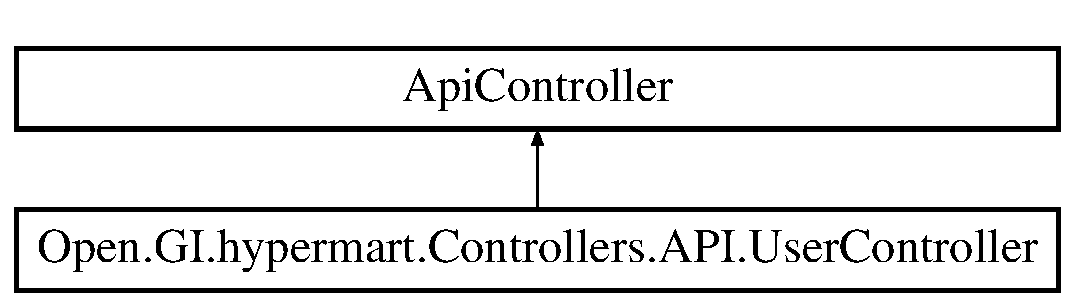
\includegraphics[height=2.000000cm]{class_open_1_1_g_i_1_1hypermart_1_1_controllers_1_1_a_p_i_1_1_user_controller}
\end{center}
\end{figure}
\subsection*{Public Member Functions}
\begin{DoxyCompactItemize}
\item 
\hyperlink{class_open_1_1_g_i_1_1hypermart_1_1_data_transformation_objects_1_1_user_d_t_o}{User\+D\+TO} \hyperlink{class_open_1_1_g_i_1_1hypermart_1_1_controllers_1_1_a_p_i_1_1_user_controller_af2896a942d750bcc948228c298221f15}{Details} (string userid)
\begin{DoxyCompactList}\small\item\em Retrieves the user information from the directory. \end{DoxyCompactList}\end{DoxyCompactItemize}


\subsection{Detailed Description}
This is the Open\+GI \hyperlink{namespace_open_1_1_g_i_1_1hypermart_1_1_controllers_1_1_a_p_i}{A\+PI} layer for interacting with users. This \hyperlink{namespace_open_1_1_g_i_1_1hypermart_1_1_controllers_1_1_a_p_i}{A\+PI} layer allows user details to be retireved from Active Directory. 

Required minimal configuration, but does require a directory services of sorts -\/ this should work with the Active Directory Lightweight Directory Services (to be confirmed). 

\subsection{Member Function Documentation}
\hypertarget{class_open_1_1_g_i_1_1hypermart_1_1_controllers_1_1_a_p_i_1_1_user_controller_af2896a942d750bcc948228c298221f15}{}\label{class_open_1_1_g_i_1_1hypermart_1_1_controllers_1_1_a_p_i_1_1_user_controller_af2896a942d750bcc948228c298221f15} 
\index{Open\+::\+G\+I\+::hypermart\+::\+Controllers\+::\+A\+P\+I\+::\+User\+Controller@{Open\+::\+G\+I\+::hypermart\+::\+Controllers\+::\+A\+P\+I\+::\+User\+Controller}!Details@{Details}}
\index{Details@{Details}!Open\+::\+G\+I\+::hypermart\+::\+Controllers\+::\+A\+P\+I\+::\+User\+Controller@{Open\+::\+G\+I\+::hypermart\+::\+Controllers\+::\+A\+P\+I\+::\+User\+Controller}}
\subsubsection{\texorpdfstring{Details()}{Details()}}
{\footnotesize\ttfamily \hyperlink{class_open_1_1_g_i_1_1hypermart_1_1_data_transformation_objects_1_1_user_d_t_o}{User\+D\+TO} Open.\+G\+I.\+hypermart.\+Controllers.\+A\+P\+I.\+User\+Controller.\+Details (\begin{DoxyParamCaption}\item[{string}]{userid }\end{DoxyParamCaption})}



Retrieves the user information from the directory. 


\begin{DoxyParams}{Parameters}
{\em userid} & \\
\hline
\end{DoxyParams}
\begin{DoxyReturn}{Returns}

\end{DoxyReturn}


The documentation for this class was generated from the following file\+:\begin{DoxyCompactItemize}
\item 
C\+:/\+Projects/\+App-\/\+Utility-\/\+Store/\+Open.\+G\+I.\+hypermart/\+Controllers/\+A\+P\+I/\hyperlink{_a_p_i_2_user_controller_8cs}{User\+Controller.\+cs}\end{DoxyCompactItemize}

\section{Open.\+G\+I.\+hypermart.\+Controllers.\+User\+Controller Class Reference}
\label{class_open_1_1_g_i_1_1hypermart_1_1_controllers_1_1_user_controller}\index{Open.\+G\+I.\+hypermart.\+Controllers.\+User\+Controller@{Open.\+G\+I.\+hypermart.\+Controllers.\+User\+Controller}}


User Controller  


Inheritance diagram for Open.\+G\+I.\+hypermart.\+Controllers.\+User\+Controller\+:\begin{figure}[H]
\begin{center}
\leavevmode
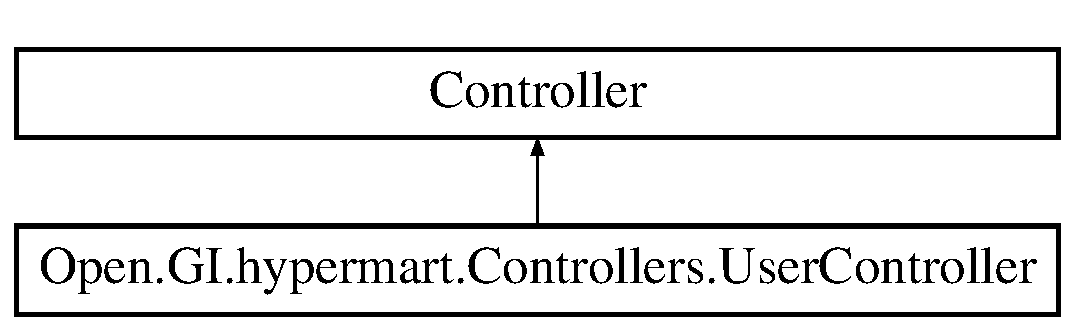
\includegraphics[height=2.000000cm]{class_open_1_1_g_i_1_1hypermart_1_1_controllers_1_1_user_controller}
\end{center}
\end{figure}
\subsection*{Public Member Functions}
\begin{DoxyCompactItemize}
\item 
Action\+Result \textbf{ Details} (string id)
\begin{DoxyCompactList}\small\item\em Detailses the specified userid. \end{DoxyCompactList}\item 
Action\+Result \textbf{ popup\+\_\+\+Details} (string userid)
\begin{DoxyCompactList}\small\item\em Detailses the specified userid. \end{DoxyCompactList}\end{DoxyCompactItemize}


\subsection{Detailed Description}
User Controller 

\begin{DoxySeeAlso}{See also}
System.\+Web.\+Mvc.\+Controller


\end{DoxySeeAlso}


Definition at line 13 of file User\+Controller.\+cs.



\subsection{Member Function Documentation}
\mbox{\label{class_open_1_1_g_i_1_1hypermart_1_1_controllers_1_1_user_controller_a4627a7a94b713760f00050bac936a54f}} 
\index{Open\+::\+G\+I\+::hypermart\+::\+Controllers\+::\+User\+Controller@{Open\+::\+G\+I\+::hypermart\+::\+Controllers\+::\+User\+Controller}!Details@{Details}}
\index{Details@{Details}!Open\+::\+G\+I\+::hypermart\+::\+Controllers\+::\+User\+Controller@{Open\+::\+G\+I\+::hypermart\+::\+Controllers\+::\+User\+Controller}}
\subsubsection{Details()}
{\footnotesize\ttfamily Action\+Result Open.\+G\+I.\+hypermart.\+Controllers.\+User\+Controller.\+Details (\begin{DoxyParamCaption}\item[{string}]{id }\end{DoxyParamCaption})}



Detailses the specified userid. 


\begin{DoxyParams}{Parameters}
{\em id} & The userid.\\
\hline
\end{DoxyParams}
\begin{DoxyReturn}{Returns}

\end{DoxyReturn}


Definition at line 28 of file User\+Controller.\+cs.

\mbox{\label{class_open_1_1_g_i_1_1hypermart_1_1_controllers_1_1_user_controller_a3168162b86edbdbd30a593fa6aca8e9f}} 
\index{Open\+::\+G\+I\+::hypermart\+::\+Controllers\+::\+User\+Controller@{Open\+::\+G\+I\+::hypermart\+::\+Controllers\+::\+User\+Controller}!popup\+\_\+\+Details@{popup\+\_\+\+Details}}
\index{popup\+\_\+\+Details@{popup\+\_\+\+Details}!Open\+::\+G\+I\+::hypermart\+::\+Controllers\+::\+User\+Controller@{Open\+::\+G\+I\+::hypermart\+::\+Controllers\+::\+User\+Controller}}
\subsubsection{popup\+\_\+\+Details()}
{\footnotesize\ttfamily Action\+Result Open.\+G\+I.\+hypermart.\+Controllers.\+User\+Controller.\+popup\+\_\+\+Details (\begin{DoxyParamCaption}\item[{string}]{userid }\end{DoxyParamCaption})}



Detailses the specified userid. 


\begin{DoxyParams}{Parameters}
{\em userid} & The userid.\\
\hline
\end{DoxyParams}
\begin{DoxyReturn}{Returns}

\end{DoxyReturn}


Definition at line 57 of file User\+Controller.\+cs.



The documentation for this class was generated from the following file\+:\begin{DoxyCompactItemize}
\item 
C\+:/\+Projects/\+App-\/\+Utility-\/\+Store/\+Open.\+G\+I.\+hypermart/\+Controllers/\textbf{ User\+Controller.\+cs}\end{DoxyCompactItemize}

\hypertarget{class_open_1_1_g_i_1_1hypermart_1_1_data_transformation_objects_1_1_user_d_t_o}{}\section{Open.\+G\+I.\+hypermart.\+Data\+Transformation\+Objects.\+User\+D\+T\+O Class Reference}
\label{class_open_1_1_g_i_1_1hypermart_1_1_data_transformation_objects_1_1_user_d_t_o}\index{Open.\+G\+I.\+hypermart.\+Data\+Transformation\+Objects.\+User\+D\+T\+O@{Open.\+G\+I.\+hypermart.\+Data\+Transformation\+Objects.\+User\+D\+T\+O}}


Class for Over-\/the-\/wire transmission of user information. If a user cannot be found, then an Unknown User will be returned.  


\subsection*{Public Member Functions}
\begin{DoxyCompactItemize}
\item 
\hyperlink{class_open_1_1_g_i_1_1hypermart_1_1_data_transformation_objects_1_1_user_d_t_o_ab715e6cac8b432f39c5fe6f22e3db645}{User\+D\+T\+O} ()
\begin{DoxyCompactList}\small\item\em Initializes a new instance of the \hyperlink{class_open_1_1_g_i_1_1hypermart_1_1_data_transformation_objects_1_1_user_d_t_o}{User\+D\+T\+O} class. \end{DoxyCompactList}\item 
\hyperlink{class_open_1_1_g_i_1_1hypermart_1_1_data_transformation_objects_1_1_user_d_t_o_a21ce2f8eaac0781bcc484f8eeca38404}{User\+D\+T\+O} (\hyperlink{class_open_1_1_g_i_1_1hypermart_1_1_models_1_1_user}{Open.\+G\+I.\+hypermart.\+Models.\+User} User\+To\+Wrap)
\begin{DoxyCompactList}\small\item\em Initializes a new instance of the \hyperlink{class_open_1_1_g_i_1_1hypermart_1_1_data_transformation_objects_1_1_user_d_t_o}{User\+D\+T\+O} class. \end{DoxyCompactList}\end{DoxyCompactItemize}
\subsection*{Properties}
\begin{DoxyCompactItemize}
\item 
string \hyperlink{class_open_1_1_g_i_1_1hypermart_1_1_data_transformation_objects_1_1_user_d_t_o_a123512619de906f987a3da0b7ec32bb1}{username}\hspace{0.3cm}{\ttfamily  \mbox{[}get, set\mbox{]}}
\begin{DoxyCompactList}\small\item\em Gets or sets the username. \end{DoxyCompactList}\item 
string \hyperlink{class_open_1_1_g_i_1_1hypermart_1_1_data_transformation_objects_1_1_user_d_t_o_a8ead06f70fbd3e0bcc72bf3aaae4fc9f}{Phone\+Numnber}\hspace{0.3cm}{\ttfamily  \mbox{[}get, set\mbox{]}}
\begin{DoxyCompactList}\small\item\em Gets or sets the phone numnber. \end{DoxyCompactList}\item 
Byte\mbox{[}$\,$\mbox{]} \hyperlink{class_open_1_1_g_i_1_1hypermart_1_1_data_transformation_objects_1_1_user_d_t_o_a3e4447b4cd2ef861c95c1e9162cbceb1}{Photo\+\_\+byte\+Array}\hspace{0.3cm}{\ttfamily  \mbox{[}get, set\mbox{]}}
\begin{DoxyCompactList}\small\item\em Base 64 encoded png image. \end{DoxyCompactList}\item 
string \hyperlink{class_open_1_1_g_i_1_1hypermart_1_1_data_transformation_objects_1_1_user_d_t_o_a96fdfcc9b2aa36fb35f6612b9e99b535}{Email}\hspace{0.3cm}{\ttfamily  \mbox{[}get, set\mbox{]}}
\begin{DoxyCompactList}\small\item\em Gets or sets the email. \end{DoxyCompactList}\item 
string \hyperlink{class_open_1_1_g_i_1_1hypermart_1_1_data_transformation_objects_1_1_user_d_t_o_a7a436dea35ee6683f2f7f0c3e9551d08}{Job\+Title}\hspace{0.3cm}{\ttfamily  \mbox{[}get, set\mbox{]}}
\begin{DoxyCompactList}\small\item\em Gets or sets the job title. \end{DoxyCompactList}\end{DoxyCompactItemize}


\subsection{Detailed Description}
Class for Over-\/the-\/wire transmission of user information. If a user cannot be found, then an Unknown User will be returned. 



Definition at line 14 of file User\+D\+T\+O.\+cs.



\subsection{Constructor \& Destructor Documentation}
\hypertarget{class_open_1_1_g_i_1_1hypermart_1_1_data_transformation_objects_1_1_user_d_t_o_ab715e6cac8b432f39c5fe6f22e3db645}{}\index{Open\+::\+G\+I\+::hypermart\+::\+Data\+Transformation\+Objects\+::\+User\+D\+T\+O@{Open\+::\+G\+I\+::hypermart\+::\+Data\+Transformation\+Objects\+::\+User\+D\+T\+O}!User\+D\+T\+O@{User\+D\+T\+O}}
\index{User\+D\+T\+O@{User\+D\+T\+O}!Open\+::\+G\+I\+::hypermart\+::\+Data\+Transformation\+Objects\+::\+User\+D\+T\+O@{Open\+::\+G\+I\+::hypermart\+::\+Data\+Transformation\+Objects\+::\+User\+D\+T\+O}}
\subsubsection[{User\+D\+T\+O()}]{\setlength{\rightskip}{0pt plus 5cm}Open.\+G\+I.\+hypermart.\+Data\+Transformation\+Objects.\+User\+D\+T\+O.\+User\+D\+T\+O (
\begin{DoxyParamCaption}
{}
\end{DoxyParamCaption}
)}\label{class_open_1_1_g_i_1_1hypermart_1_1_data_transformation_objects_1_1_user_d_t_o_ab715e6cac8b432f39c5fe6f22e3db645}


Initializes a new instance of the \hyperlink{class_open_1_1_g_i_1_1hypermart_1_1_data_transformation_objects_1_1_user_d_t_o}{User\+D\+T\+O} class. 



Definition at line 19 of file User\+D\+T\+O.\+cs.

\hypertarget{class_open_1_1_g_i_1_1hypermart_1_1_data_transformation_objects_1_1_user_d_t_o_a21ce2f8eaac0781bcc484f8eeca38404}{}\index{Open\+::\+G\+I\+::hypermart\+::\+Data\+Transformation\+Objects\+::\+User\+D\+T\+O@{Open\+::\+G\+I\+::hypermart\+::\+Data\+Transformation\+Objects\+::\+User\+D\+T\+O}!User\+D\+T\+O@{User\+D\+T\+O}}
\index{User\+D\+T\+O@{User\+D\+T\+O}!Open\+::\+G\+I\+::hypermart\+::\+Data\+Transformation\+Objects\+::\+User\+D\+T\+O@{Open\+::\+G\+I\+::hypermart\+::\+Data\+Transformation\+Objects\+::\+User\+D\+T\+O}}
\subsubsection[{User\+D\+T\+O(\+Open.\+G\+I.\+hypermart.\+Models.\+User User\+To\+Wrap)}]{\setlength{\rightskip}{0pt plus 5cm}Open.\+G\+I.\+hypermart.\+Data\+Transformation\+Objects.\+User\+D\+T\+O.\+User\+D\+T\+O (
\begin{DoxyParamCaption}
\item[{{\bf Open.\+G\+I.\+hypermart.\+Models.\+User}}]{User\+To\+Wrap}
\end{DoxyParamCaption}
)}\label{class_open_1_1_g_i_1_1hypermart_1_1_data_transformation_objects_1_1_user_d_t_o_a21ce2f8eaac0781bcc484f8eeca38404}


Initializes a new instance of the \hyperlink{class_open_1_1_g_i_1_1hypermart_1_1_data_transformation_objects_1_1_user_d_t_o}{User\+D\+T\+O} class. 


\begin{DoxyParams}{Parameters}
{\em User\+To\+Wrap} & The user to wrap.\\
\hline
\end{DoxyParams}


Definition at line 28 of file User\+D\+T\+O.\+cs.



\subsection{Property Documentation}
\hypertarget{class_open_1_1_g_i_1_1hypermart_1_1_data_transformation_objects_1_1_user_d_t_o_a96fdfcc9b2aa36fb35f6612b9e99b535}{}\index{Open\+::\+G\+I\+::hypermart\+::\+Data\+Transformation\+Objects\+::\+User\+D\+T\+O@{Open\+::\+G\+I\+::hypermart\+::\+Data\+Transformation\+Objects\+::\+User\+D\+T\+O}!Email@{Email}}
\index{Email@{Email}!Open\+::\+G\+I\+::hypermart\+::\+Data\+Transformation\+Objects\+::\+User\+D\+T\+O@{Open\+::\+G\+I\+::hypermart\+::\+Data\+Transformation\+Objects\+::\+User\+D\+T\+O}}
\subsubsection[{Email}]{\setlength{\rightskip}{0pt plus 5cm}string Open.\+G\+I.\+hypermart.\+Data\+Transformation\+Objects.\+User\+D\+T\+O.\+Email\hspace{0.3cm}{\ttfamily [get]}, {\ttfamily [set]}}\label{class_open_1_1_g_i_1_1hypermart_1_1_data_transformation_objects_1_1_user_d_t_o_a96fdfcc9b2aa36fb35f6612b9e99b535}


Gets or sets the email. 

The email. 

Definition at line 60 of file User\+D\+T\+O.\+cs.

\hypertarget{class_open_1_1_g_i_1_1hypermart_1_1_data_transformation_objects_1_1_user_d_t_o_a7a436dea35ee6683f2f7f0c3e9551d08}{}\index{Open\+::\+G\+I\+::hypermart\+::\+Data\+Transformation\+Objects\+::\+User\+D\+T\+O@{Open\+::\+G\+I\+::hypermart\+::\+Data\+Transformation\+Objects\+::\+User\+D\+T\+O}!Job\+Title@{Job\+Title}}
\index{Job\+Title@{Job\+Title}!Open\+::\+G\+I\+::hypermart\+::\+Data\+Transformation\+Objects\+::\+User\+D\+T\+O@{Open\+::\+G\+I\+::hypermart\+::\+Data\+Transformation\+Objects\+::\+User\+D\+T\+O}}
\subsubsection[{Job\+Title}]{\setlength{\rightskip}{0pt plus 5cm}string Open.\+G\+I.\+hypermart.\+Data\+Transformation\+Objects.\+User\+D\+T\+O.\+Job\+Title\hspace{0.3cm}{\ttfamily [get]}, {\ttfamily [set]}}\label{class_open_1_1_g_i_1_1hypermart_1_1_data_transformation_objects_1_1_user_d_t_o_a7a436dea35ee6683f2f7f0c3e9551d08}


Gets or sets the job title. 

The job title. 

Definition at line 67 of file User\+D\+T\+O.\+cs.

\hypertarget{class_open_1_1_g_i_1_1hypermart_1_1_data_transformation_objects_1_1_user_d_t_o_a8ead06f70fbd3e0bcc72bf3aaae4fc9f}{}\index{Open\+::\+G\+I\+::hypermart\+::\+Data\+Transformation\+Objects\+::\+User\+D\+T\+O@{Open\+::\+G\+I\+::hypermart\+::\+Data\+Transformation\+Objects\+::\+User\+D\+T\+O}!Phone\+Numnber@{Phone\+Numnber}}
\index{Phone\+Numnber@{Phone\+Numnber}!Open\+::\+G\+I\+::hypermart\+::\+Data\+Transformation\+Objects\+::\+User\+D\+T\+O@{Open\+::\+G\+I\+::hypermart\+::\+Data\+Transformation\+Objects\+::\+User\+D\+T\+O}}
\subsubsection[{Phone\+Numnber}]{\setlength{\rightskip}{0pt plus 5cm}string Open.\+G\+I.\+hypermart.\+Data\+Transformation\+Objects.\+User\+D\+T\+O.\+Phone\+Numnber\hspace{0.3cm}{\ttfamily [get]}, {\ttfamily [set]}}\label{class_open_1_1_g_i_1_1hypermart_1_1_data_transformation_objects_1_1_user_d_t_o_a8ead06f70fbd3e0bcc72bf3aaae4fc9f}


Gets or sets the phone numnber. 

The phone numnber. 

Definition at line 49 of file User\+D\+T\+O.\+cs.

\hypertarget{class_open_1_1_g_i_1_1hypermart_1_1_data_transformation_objects_1_1_user_d_t_o_a3e4447b4cd2ef861c95c1e9162cbceb1}{}\index{Open\+::\+G\+I\+::hypermart\+::\+Data\+Transformation\+Objects\+::\+User\+D\+T\+O@{Open\+::\+G\+I\+::hypermart\+::\+Data\+Transformation\+Objects\+::\+User\+D\+T\+O}!Photo\+\_\+byte\+Array@{Photo\+\_\+byte\+Array}}
\index{Photo\+\_\+byte\+Array@{Photo\+\_\+byte\+Array}!Open\+::\+G\+I\+::hypermart\+::\+Data\+Transformation\+Objects\+::\+User\+D\+T\+O@{Open\+::\+G\+I\+::hypermart\+::\+Data\+Transformation\+Objects\+::\+User\+D\+T\+O}}
\subsubsection[{Photo\+\_\+byte\+Array}]{\setlength{\rightskip}{0pt plus 5cm}Byte \mbox{[}$\,$\mbox{]} Open.\+G\+I.\+hypermart.\+Data\+Transformation\+Objects.\+User\+D\+T\+O.\+Photo\+\_\+byte\+Array\hspace{0.3cm}{\ttfamily [get]}, {\ttfamily [set]}}\label{class_open_1_1_g_i_1_1hypermart_1_1_data_transformation_objects_1_1_user_d_t_o_a3e4447b4cd2ef861c95c1e9162cbceb1}


Base 64 encoded png image. 



Definition at line 53 of file User\+D\+T\+O.\+cs.

\hypertarget{class_open_1_1_g_i_1_1hypermart_1_1_data_transformation_objects_1_1_user_d_t_o_a123512619de906f987a3da0b7ec32bb1}{}\index{Open\+::\+G\+I\+::hypermart\+::\+Data\+Transformation\+Objects\+::\+User\+D\+T\+O@{Open\+::\+G\+I\+::hypermart\+::\+Data\+Transformation\+Objects\+::\+User\+D\+T\+O}!username@{username}}
\index{username@{username}!Open\+::\+G\+I\+::hypermart\+::\+Data\+Transformation\+Objects\+::\+User\+D\+T\+O@{Open\+::\+G\+I\+::hypermart\+::\+Data\+Transformation\+Objects\+::\+User\+D\+T\+O}}
\subsubsection[{username}]{\setlength{\rightskip}{0pt plus 5cm}string Open.\+G\+I.\+hypermart.\+Data\+Transformation\+Objects.\+User\+D\+T\+O.\+username\hspace{0.3cm}{\ttfamily [get]}, {\ttfamily [set]}}\label{class_open_1_1_g_i_1_1hypermart_1_1_data_transformation_objects_1_1_user_d_t_o_a123512619de906f987a3da0b7ec32bb1}


Gets or sets the username. 

The username. 

Definition at line 42 of file User\+D\+T\+O.\+cs.



The documentation for this class was generated from the following file\+:\begin{DoxyCompactItemize}
\item 
C\+:/\+Projects/\+App-\/\+Utility-\/\+Store/\+Open.\+G\+I.\+hypermart/\+Data\+Transformation\+Objects/\hyperlink{_user_d_t_o_8cs}{User\+D\+T\+O.\+cs}\end{DoxyCompactItemize}

\hypertarget{class_open_1_1_g_i_1_1hypermart_1_1_controllers_1_1_a_p_i_1_1_values_controller1}{}\section{Open.\+G\+I.\+hypermart.\+Controllers.\+A\+P\+I.\+Values\+Controller1 Class Reference}
\label{class_open_1_1_g_i_1_1hypermart_1_1_controllers_1_1_a_p_i_1_1_values_controller1}\index{Open.\+G\+I.\+hypermart.\+Controllers.\+A\+P\+I.\+Values\+Controller1@{Open.\+G\+I.\+hypermart.\+Controllers.\+A\+P\+I.\+Values\+Controller1}}


Values Controller  


Inheritance diagram for Open.\+G\+I.\+hypermart.\+Controllers.\+A\+P\+I.\+Values\+Controller1\+:\begin{figure}[H]
\begin{center}
\leavevmode
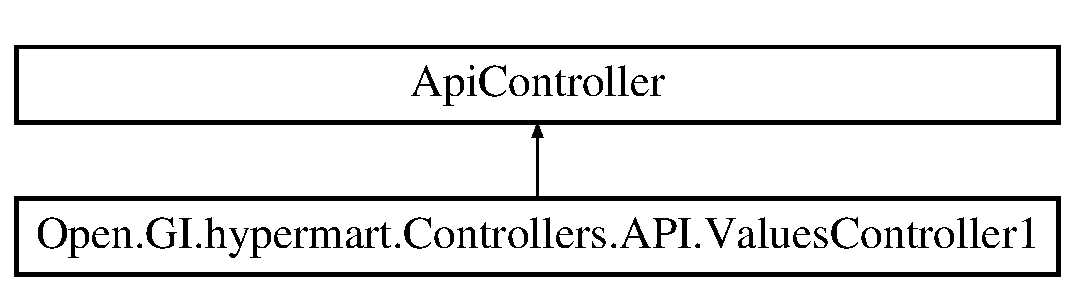
\includegraphics[height=2.000000cm]{class_open_1_1_g_i_1_1hypermart_1_1_controllers_1_1_a_p_i_1_1_values_controller1}
\end{center}
\end{figure}
\subsection*{Public Member Functions}
\begin{DoxyCompactItemize}
\item 
I\+Enumerable$<$ string $>$ \hyperlink{class_open_1_1_g_i_1_1hypermart_1_1_controllers_1_1_a_p_i_1_1_values_controller1_a8a5f7b7ca76cec5f41e04cca6ecddb3e}{Get} ()
\begin{DoxyCompactList}\small\item\em Gets all of the values \end{DoxyCompactList}\item 
string \hyperlink{class_open_1_1_g_i_1_1hypermart_1_1_controllers_1_1_a_p_i_1_1_values_controller1_a4474d8ac7e57e5c271f44870b0836259}{Get} (int id)
\begin{DoxyCompactList}\small\item\em Gets the specified identifier. \end{DoxyCompactList}\item 
void \hyperlink{class_open_1_1_g_i_1_1hypermart_1_1_controllers_1_1_a_p_i_1_1_values_controller1_a36f57a403289840e0545d8ba47ea04d2}{Post} (\mbox{[}From\+Body\mbox{]}string value)
\begin{DoxyCompactList}\small\item\em Posts the specified value. \end{DoxyCompactList}\item 
void \hyperlink{class_open_1_1_g_i_1_1hypermart_1_1_controllers_1_1_a_p_i_1_1_values_controller1_abc6ccf3b8af53263011cb0c7788dd69c}{Put} (int id, \mbox{[}From\+Body\mbox{]}string value)
\begin{DoxyCompactList}\small\item\em Puts the specified identifier. \end{DoxyCompactList}\item 
void \hyperlink{class_open_1_1_g_i_1_1hypermart_1_1_controllers_1_1_a_p_i_1_1_values_controller1_a90c5ec51ac779bf121442d6329938ee0}{Delete} (int id)
\begin{DoxyCompactList}\small\item\em Deletes the specified identifier. \end{DoxyCompactList}\end{DoxyCompactItemize}


\subsection{Detailed Description}
Values Controller 

\begin{DoxySeeAlso}{See also}
System.\+Web.\+Http.\+Api\+Controller


\end{DoxySeeAlso}


Definition at line 14 of file Values\+Controller1.\+cs.



\subsection{Member Function Documentation}
\hypertarget{class_open_1_1_g_i_1_1hypermart_1_1_controllers_1_1_a_p_i_1_1_values_controller1_a90c5ec51ac779bf121442d6329938ee0}{}\index{Open\+::\+G\+I\+::hypermart\+::\+Controllers\+::\+A\+P\+I\+::\+Values\+Controller1@{Open\+::\+G\+I\+::hypermart\+::\+Controllers\+::\+A\+P\+I\+::\+Values\+Controller1}!Delete@{Delete}}
\index{Delete@{Delete}!Open\+::\+G\+I\+::hypermart\+::\+Controllers\+::\+A\+P\+I\+::\+Values\+Controller1@{Open\+::\+G\+I\+::hypermart\+::\+Controllers\+::\+A\+P\+I\+::\+Values\+Controller1}}
\subsubsection[{Delete(int id)}]{\setlength{\rightskip}{0pt plus 5cm}void Open.\+G\+I.\+hypermart.\+Controllers.\+A\+P\+I.\+Values\+Controller1.\+Delete (
\begin{DoxyParamCaption}
\item[{int}]{id}
\end{DoxyParamCaption}
)}\label{class_open_1_1_g_i_1_1hypermart_1_1_controllers_1_1_a_p_i_1_1_values_controller1_a90c5ec51ac779bf121442d6329938ee0}


Deletes the specified identifier. 


\begin{DoxyParams}{Parameters}
{\em id} & The identifier.\\
\hline
\end{DoxyParams}


Definition at line 56 of file Values\+Controller1.\+cs.

\hypertarget{class_open_1_1_g_i_1_1hypermart_1_1_controllers_1_1_a_p_i_1_1_values_controller1_a8a5f7b7ca76cec5f41e04cca6ecddb3e}{}\index{Open\+::\+G\+I\+::hypermart\+::\+Controllers\+::\+A\+P\+I\+::\+Values\+Controller1@{Open\+::\+G\+I\+::hypermart\+::\+Controllers\+::\+A\+P\+I\+::\+Values\+Controller1}!Get@{Get}}
\index{Get@{Get}!Open\+::\+G\+I\+::hypermart\+::\+Controllers\+::\+A\+P\+I\+::\+Values\+Controller1@{Open\+::\+G\+I\+::hypermart\+::\+Controllers\+::\+A\+P\+I\+::\+Values\+Controller1}}
\subsubsection[{Get()}]{\setlength{\rightskip}{0pt plus 5cm}I\+Enumerable$<$string$>$ Open.\+G\+I.\+hypermart.\+Controllers.\+A\+P\+I.\+Values\+Controller1.\+Get (
\begin{DoxyParamCaption}
{}
\end{DoxyParamCaption}
)}\label{class_open_1_1_g_i_1_1hypermart_1_1_controllers_1_1_a_p_i_1_1_values_controller1_a8a5f7b7ca76cec5f41e04cca6ecddb3e}


Gets all of the values 

\begin{DoxyReturn}{Returns}

\end{DoxyReturn}


Definition at line 20 of file Values\+Controller1.\+cs.

\hypertarget{class_open_1_1_g_i_1_1hypermart_1_1_controllers_1_1_a_p_i_1_1_values_controller1_a4474d8ac7e57e5c271f44870b0836259}{}\index{Open\+::\+G\+I\+::hypermart\+::\+Controllers\+::\+A\+P\+I\+::\+Values\+Controller1@{Open\+::\+G\+I\+::hypermart\+::\+Controllers\+::\+A\+P\+I\+::\+Values\+Controller1}!Get@{Get}}
\index{Get@{Get}!Open\+::\+G\+I\+::hypermart\+::\+Controllers\+::\+A\+P\+I\+::\+Values\+Controller1@{Open\+::\+G\+I\+::hypermart\+::\+Controllers\+::\+A\+P\+I\+::\+Values\+Controller1}}
\subsubsection[{Get(int id)}]{\setlength{\rightskip}{0pt plus 5cm}string Open.\+G\+I.\+hypermart.\+Controllers.\+A\+P\+I.\+Values\+Controller1.\+Get (
\begin{DoxyParamCaption}
\item[{int}]{id}
\end{DoxyParamCaption}
)}\label{class_open_1_1_g_i_1_1hypermart_1_1_controllers_1_1_a_p_i_1_1_values_controller1_a4474d8ac7e57e5c271f44870b0836259}


Gets the specified identifier. 


\begin{DoxyParams}{Parameters}
{\em id} & The identifier.\\
\hline
\end{DoxyParams}
\begin{DoxyReturn}{Returns}

\end{DoxyReturn}


Definition at line 30 of file Values\+Controller1.\+cs.

\hypertarget{class_open_1_1_g_i_1_1hypermart_1_1_controllers_1_1_a_p_i_1_1_values_controller1_a36f57a403289840e0545d8ba47ea04d2}{}\index{Open\+::\+G\+I\+::hypermart\+::\+Controllers\+::\+A\+P\+I\+::\+Values\+Controller1@{Open\+::\+G\+I\+::hypermart\+::\+Controllers\+::\+A\+P\+I\+::\+Values\+Controller1}!Post@{Post}}
\index{Post@{Post}!Open\+::\+G\+I\+::hypermart\+::\+Controllers\+::\+A\+P\+I\+::\+Values\+Controller1@{Open\+::\+G\+I\+::hypermart\+::\+Controllers\+::\+A\+P\+I\+::\+Values\+Controller1}}
\subsubsection[{Post([From\+Body]string value)}]{\setlength{\rightskip}{0pt plus 5cm}void Open.\+G\+I.\+hypermart.\+Controllers.\+A\+P\+I.\+Values\+Controller1.\+Post (
\begin{DoxyParamCaption}
\item[{\mbox{[}\+From\+Body\mbox{]} string}]{value}
\end{DoxyParamCaption}
)}\label{class_open_1_1_g_i_1_1hypermart_1_1_controllers_1_1_a_p_i_1_1_values_controller1_a36f57a403289840e0545d8ba47ea04d2}


Posts the specified value. 


\begin{DoxyParams}{Parameters}
{\em value} & The value.\\
\hline
\end{DoxyParams}


Definition at line 39 of file Values\+Controller1.\+cs.

\hypertarget{class_open_1_1_g_i_1_1hypermart_1_1_controllers_1_1_a_p_i_1_1_values_controller1_abc6ccf3b8af53263011cb0c7788dd69c}{}\index{Open\+::\+G\+I\+::hypermart\+::\+Controllers\+::\+A\+P\+I\+::\+Values\+Controller1@{Open\+::\+G\+I\+::hypermart\+::\+Controllers\+::\+A\+P\+I\+::\+Values\+Controller1}!Put@{Put}}
\index{Put@{Put}!Open\+::\+G\+I\+::hypermart\+::\+Controllers\+::\+A\+P\+I\+::\+Values\+Controller1@{Open\+::\+G\+I\+::hypermart\+::\+Controllers\+::\+A\+P\+I\+::\+Values\+Controller1}}
\subsubsection[{Put(int id, [From\+Body]string value)}]{\setlength{\rightskip}{0pt plus 5cm}void Open.\+G\+I.\+hypermart.\+Controllers.\+A\+P\+I.\+Values\+Controller1.\+Put (
\begin{DoxyParamCaption}
\item[{int}]{id, }
\item[{\mbox{[}\+From\+Body\mbox{]} string}]{value}
\end{DoxyParamCaption}
)}\label{class_open_1_1_g_i_1_1hypermart_1_1_controllers_1_1_a_p_i_1_1_values_controller1_abc6ccf3b8af53263011cb0c7788dd69c}


Puts the specified identifier. 


\begin{DoxyParams}{Parameters}
{\em id} & The identifier.\\
\hline
{\em value} & The value.\\
\hline
\end{DoxyParams}


Definition at line 48 of file Values\+Controller1.\+cs.



The documentation for this class was generated from the following file\+:\begin{DoxyCompactItemize}
\item 
C\+:/\+Projects/\+App-\/\+Utility-\/\+Store/\+Open.\+G\+I.\+hypermart/\+Controllers/\+A\+P\+I/\hyperlink{_values_controller1_8cs}{Values\+Controller1.\+cs}\end{DoxyCompactItemize}

\hypertarget{class_open_1_1_g_i_1_1hypermart_1_1_areas_1_1_help_page_1_1_xml_documentation_provider}{}\section{Open.\+G\+I.\+hypermart.\+Areas.\+Help\+Page.\+Xml\+Documentation\+Provider Class Reference}
\label{class_open_1_1_g_i_1_1hypermart_1_1_areas_1_1_help_page_1_1_xml_documentation_provider}\index{Open.\+G\+I.\+hypermart.\+Areas.\+Help\+Page.\+Xml\+Documentation\+Provider@{Open.\+G\+I.\+hypermart.\+Areas.\+Help\+Page.\+Xml\+Documentation\+Provider}}


A custom I\+Documentation\+Provider that reads the A\+P\+I documentation from an X\+M\+L documentation file.  


Inheritance diagram for Open.\+G\+I.\+hypermart.\+Areas.\+Help\+Page.\+Xml\+Documentation\+Provider\+:\begin{figure}[H]
\begin{center}
\leavevmode
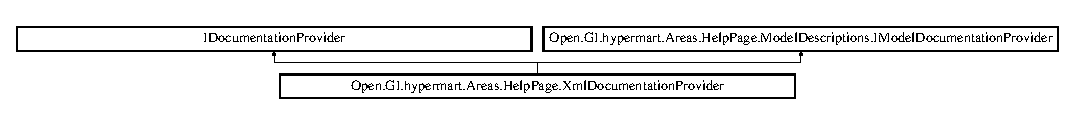
\includegraphics[height=1.102362cm]{class_open_1_1_g_i_1_1hypermart_1_1_areas_1_1_help_page_1_1_xml_documentation_provider}
\end{center}
\end{figure}
\subsection*{Public Member Functions}
\begin{DoxyCompactItemize}
\item 
\hyperlink{class_open_1_1_g_i_1_1hypermart_1_1_areas_1_1_help_page_1_1_xml_documentation_provider_a20855501bd3ff394652127b70e822308}{Xml\+Documentation\+Provider} (string document\+Path)
\begin{DoxyCompactList}\small\item\em Initializes a new instance of the \hyperlink{class_open_1_1_g_i_1_1hypermart_1_1_areas_1_1_help_page_1_1_xml_documentation_provider}{Xml\+Documentation\+Provider} class. \end{DoxyCompactList}\item 
string \hyperlink{class_open_1_1_g_i_1_1hypermart_1_1_areas_1_1_help_page_1_1_xml_documentation_provider_a05e11e0de4ff25a0e602ce9e5e916056}{Get\+Documentation} (Http\+Controller\+Descriptor controller\+Descriptor)
\begin{DoxyCompactList}\small\item\em Gets the documentation. \end{DoxyCompactList}\item 
virtual string \hyperlink{class_open_1_1_g_i_1_1hypermart_1_1_areas_1_1_help_page_1_1_xml_documentation_provider_ad27b3bee09fd9709d46eb720bff4b860}{Get\+Documentation} (Http\+Action\+Descriptor action\+Descriptor)
\begin{DoxyCompactList}\small\item\em Gets the documentation based on T\+:\+System.\+Web.\+Http.\+Controllers.\+Http\+Action\+Descriptor. \end{DoxyCompactList}\item 
virtual string \hyperlink{class_open_1_1_g_i_1_1hypermart_1_1_areas_1_1_help_page_1_1_xml_documentation_provider_a765e1ebc7e331274a664dd0edba7660c}{Get\+Documentation} (Http\+Parameter\+Descriptor parameter\+Descriptor)
\begin{DoxyCompactList}\small\item\em Gets the documentation based on T\+:\+System.\+Web.\+Http.\+Controllers.\+Http\+Parameter\+Descriptor. \end{DoxyCompactList}\item 
string \hyperlink{class_open_1_1_g_i_1_1hypermart_1_1_areas_1_1_help_page_1_1_xml_documentation_provider_a3f8e45cb0b20d0aef5e795a7ac638346}{Get\+Response\+Documentation} (Http\+Action\+Descriptor action\+Descriptor)
\begin{DoxyCompactList}\small\item\em Gets the response documentation. \end{DoxyCompactList}\item 
string \hyperlink{class_open_1_1_g_i_1_1hypermart_1_1_areas_1_1_help_page_1_1_xml_documentation_provider_a1ba7e50dea71787a555f92306ec99efc}{Get\+Documentation} (Member\+Info member)
\begin{DoxyCompactList}\small\item\em Gets the documentation. \end{DoxyCompactList}\item 
string \hyperlink{class_open_1_1_g_i_1_1hypermart_1_1_areas_1_1_help_page_1_1_xml_documentation_provider_af096939cdb4e5a26bd20ae3341fad66c}{Get\+Documentation} (Type type)
\begin{DoxyCompactList}\small\item\em Gets the documentation. \end{DoxyCompactList}\end{DoxyCompactItemize}


\subsection{Detailed Description}
A custom I\+Documentation\+Provider that reads the A\+P\+I documentation from an X\+M\+L documentation file. 



Definition at line 15 of file Xml\+Documentation\+Provider.\+cs.



\subsection{Constructor \& Destructor Documentation}
\hypertarget{class_open_1_1_g_i_1_1hypermart_1_1_areas_1_1_help_page_1_1_xml_documentation_provider_a20855501bd3ff394652127b70e822308}{}\index{Open\+::\+G\+I\+::hypermart\+::\+Areas\+::\+Help\+Page\+::\+Xml\+Documentation\+Provider@{Open\+::\+G\+I\+::hypermart\+::\+Areas\+::\+Help\+Page\+::\+Xml\+Documentation\+Provider}!Xml\+Documentation\+Provider@{Xml\+Documentation\+Provider}}
\index{Xml\+Documentation\+Provider@{Xml\+Documentation\+Provider}!Open\+::\+G\+I\+::hypermart\+::\+Areas\+::\+Help\+Page\+::\+Xml\+Documentation\+Provider@{Open\+::\+G\+I\+::hypermart\+::\+Areas\+::\+Help\+Page\+::\+Xml\+Documentation\+Provider}}
\subsubsection[{Xml\+Documentation\+Provider(string document\+Path)}]{\setlength{\rightskip}{0pt plus 5cm}Open.\+G\+I.\+hypermart.\+Areas.\+Help\+Page.\+Xml\+Documentation\+Provider.\+Xml\+Documentation\+Provider (
\begin{DoxyParamCaption}
\item[{string}]{document\+Path}
\end{DoxyParamCaption}
)}\label{class_open_1_1_g_i_1_1hypermart_1_1_areas_1_1_help_page_1_1_xml_documentation_provider_a20855501bd3ff394652127b70e822308}


Initializes a new instance of the \hyperlink{class_open_1_1_g_i_1_1hypermart_1_1_areas_1_1_help_page_1_1_xml_documentation_provider}{Xml\+Documentation\+Provider} class. 


\begin{DoxyParams}{Parameters}
{\em document\+Path} & The physical path to X\+M\+L document.\\
\hline
\end{DoxyParams}


Definition at line 28 of file Xml\+Documentation\+Provider.\+cs.



\subsection{Member Function Documentation}
\hypertarget{class_open_1_1_g_i_1_1hypermart_1_1_areas_1_1_help_page_1_1_xml_documentation_provider_a05e11e0de4ff25a0e602ce9e5e916056}{}\index{Open\+::\+G\+I\+::hypermart\+::\+Areas\+::\+Help\+Page\+::\+Xml\+Documentation\+Provider@{Open\+::\+G\+I\+::hypermart\+::\+Areas\+::\+Help\+Page\+::\+Xml\+Documentation\+Provider}!Get\+Documentation@{Get\+Documentation}}
\index{Get\+Documentation@{Get\+Documentation}!Open\+::\+G\+I\+::hypermart\+::\+Areas\+::\+Help\+Page\+::\+Xml\+Documentation\+Provider@{Open\+::\+G\+I\+::hypermart\+::\+Areas\+::\+Help\+Page\+::\+Xml\+Documentation\+Provider}}
\subsubsection[{Get\+Documentation(\+Http\+Controller\+Descriptor controller\+Descriptor)}]{\setlength{\rightskip}{0pt plus 5cm}string Open.\+G\+I.\+hypermart.\+Areas.\+Help\+Page.\+Xml\+Documentation\+Provider.\+Get\+Documentation (
\begin{DoxyParamCaption}
\item[{Http\+Controller\+Descriptor}]{controller\+Descriptor}
\end{DoxyParamCaption}
)}\label{class_open_1_1_g_i_1_1hypermart_1_1_areas_1_1_help_page_1_1_xml_documentation_provider_a05e11e0de4ff25a0e602ce9e5e916056}


Gets the documentation. 


\begin{DoxyParams}{Parameters}
{\em controller\+Descriptor} & The controller descriptor.\\
\hline
\end{DoxyParams}
\begin{DoxyReturn}{Returns}

\end{DoxyReturn}


Definition at line 43 of file Xml\+Documentation\+Provider.\+cs.

\hypertarget{class_open_1_1_g_i_1_1hypermart_1_1_areas_1_1_help_page_1_1_xml_documentation_provider_ad27b3bee09fd9709d46eb720bff4b860}{}\index{Open\+::\+G\+I\+::hypermart\+::\+Areas\+::\+Help\+Page\+::\+Xml\+Documentation\+Provider@{Open\+::\+G\+I\+::hypermart\+::\+Areas\+::\+Help\+Page\+::\+Xml\+Documentation\+Provider}!Get\+Documentation@{Get\+Documentation}}
\index{Get\+Documentation@{Get\+Documentation}!Open\+::\+G\+I\+::hypermart\+::\+Areas\+::\+Help\+Page\+::\+Xml\+Documentation\+Provider@{Open\+::\+G\+I\+::hypermart\+::\+Areas\+::\+Help\+Page\+::\+Xml\+Documentation\+Provider}}
\subsubsection[{Get\+Documentation(\+Http\+Action\+Descriptor action\+Descriptor)}]{\setlength{\rightskip}{0pt plus 5cm}virtual string Open.\+G\+I.\+hypermart.\+Areas.\+Help\+Page.\+Xml\+Documentation\+Provider.\+Get\+Documentation (
\begin{DoxyParamCaption}
\item[{Http\+Action\+Descriptor}]{action\+Descriptor}
\end{DoxyParamCaption}
)\hspace{0.3cm}{\ttfamily [virtual]}}\label{class_open_1_1_g_i_1_1hypermart_1_1_areas_1_1_help_page_1_1_xml_documentation_provider_ad27b3bee09fd9709d46eb720bff4b860}


Gets the documentation based on T\+:\+System.\+Web.\+Http.\+Controllers.\+Http\+Action\+Descriptor. 


\begin{DoxyParams}{Parameters}
{\em action\+Descriptor} & The action descriptor.\\
\hline
\end{DoxyParams}
\begin{DoxyReturn}{Returns}
The documentation for the controller. 
\end{DoxyReturn}


Definition at line 56 of file Xml\+Documentation\+Provider.\+cs.

\hypertarget{class_open_1_1_g_i_1_1hypermart_1_1_areas_1_1_help_page_1_1_xml_documentation_provider_a765e1ebc7e331274a664dd0edba7660c}{}\index{Open\+::\+G\+I\+::hypermart\+::\+Areas\+::\+Help\+Page\+::\+Xml\+Documentation\+Provider@{Open\+::\+G\+I\+::hypermart\+::\+Areas\+::\+Help\+Page\+::\+Xml\+Documentation\+Provider}!Get\+Documentation@{Get\+Documentation}}
\index{Get\+Documentation@{Get\+Documentation}!Open\+::\+G\+I\+::hypermart\+::\+Areas\+::\+Help\+Page\+::\+Xml\+Documentation\+Provider@{Open\+::\+G\+I\+::hypermart\+::\+Areas\+::\+Help\+Page\+::\+Xml\+Documentation\+Provider}}
\subsubsection[{Get\+Documentation(\+Http\+Parameter\+Descriptor parameter\+Descriptor)}]{\setlength{\rightskip}{0pt plus 5cm}virtual string Open.\+G\+I.\+hypermart.\+Areas.\+Help\+Page.\+Xml\+Documentation\+Provider.\+Get\+Documentation (
\begin{DoxyParamCaption}
\item[{Http\+Parameter\+Descriptor}]{parameter\+Descriptor}
\end{DoxyParamCaption}
)\hspace{0.3cm}{\ttfamily [virtual]}}\label{class_open_1_1_g_i_1_1hypermart_1_1_areas_1_1_help_page_1_1_xml_documentation_provider_a765e1ebc7e331274a664dd0edba7660c}


Gets the documentation based on T\+:\+System.\+Web.\+Http.\+Controllers.\+Http\+Parameter\+Descriptor. 


\begin{DoxyParams}{Parameters}
{\em parameter\+Descriptor} & The parameter descriptor.\\
\hline
\end{DoxyParams}
\begin{DoxyReturn}{Returns}
The documentation for the controller. 
\end{DoxyReturn}


Definition at line 69 of file Xml\+Documentation\+Provider.\+cs.

\hypertarget{class_open_1_1_g_i_1_1hypermart_1_1_areas_1_1_help_page_1_1_xml_documentation_provider_a1ba7e50dea71787a555f92306ec99efc}{}\index{Open\+::\+G\+I\+::hypermart\+::\+Areas\+::\+Help\+Page\+::\+Xml\+Documentation\+Provider@{Open\+::\+G\+I\+::hypermart\+::\+Areas\+::\+Help\+Page\+::\+Xml\+Documentation\+Provider}!Get\+Documentation@{Get\+Documentation}}
\index{Get\+Documentation@{Get\+Documentation}!Open\+::\+G\+I\+::hypermart\+::\+Areas\+::\+Help\+Page\+::\+Xml\+Documentation\+Provider@{Open\+::\+G\+I\+::hypermart\+::\+Areas\+::\+Help\+Page\+::\+Xml\+Documentation\+Provider}}
\subsubsection[{Get\+Documentation(\+Member\+Info member)}]{\setlength{\rightskip}{0pt plus 5cm}string Open.\+G\+I.\+hypermart.\+Areas.\+Help\+Page.\+Xml\+Documentation\+Provider.\+Get\+Documentation (
\begin{DoxyParamCaption}
\item[{Member\+Info}]{member}
\end{DoxyParamCaption}
)}\label{class_open_1_1_g_i_1_1hypermart_1_1_areas_1_1_help_page_1_1_xml_documentation_provider_a1ba7e50dea71787a555f92306ec99efc}


Gets the documentation. 


\begin{DoxyParams}{Parameters}
{\em member} & The member.\\
\hline
\end{DoxyParams}
\begin{DoxyReturn}{Returns}

\end{DoxyReturn}


Implements \hyperlink{interface_open_1_1_g_i_1_1hypermart_1_1_areas_1_1_help_page_1_1_model_descriptions_1_1_i_model_documentation_provider_a27d4470da05e52051ae345515c17755a}{Open.\+G\+I.\+hypermart.\+Areas.\+Help\+Page.\+Model\+Descriptions.\+I\+Model\+Documentation\+Provider}.



Definition at line 105 of file Xml\+Documentation\+Provider.\+cs.

\hypertarget{class_open_1_1_g_i_1_1hypermart_1_1_areas_1_1_help_page_1_1_xml_documentation_provider_af096939cdb4e5a26bd20ae3341fad66c}{}\index{Open\+::\+G\+I\+::hypermart\+::\+Areas\+::\+Help\+Page\+::\+Xml\+Documentation\+Provider@{Open\+::\+G\+I\+::hypermart\+::\+Areas\+::\+Help\+Page\+::\+Xml\+Documentation\+Provider}!Get\+Documentation@{Get\+Documentation}}
\index{Get\+Documentation@{Get\+Documentation}!Open\+::\+G\+I\+::hypermart\+::\+Areas\+::\+Help\+Page\+::\+Xml\+Documentation\+Provider@{Open\+::\+G\+I\+::hypermart\+::\+Areas\+::\+Help\+Page\+::\+Xml\+Documentation\+Provider}}
\subsubsection[{Get\+Documentation(\+Type type)}]{\setlength{\rightskip}{0pt plus 5cm}string Open.\+G\+I.\+hypermart.\+Areas.\+Help\+Page.\+Xml\+Documentation\+Provider.\+Get\+Documentation (
\begin{DoxyParamCaption}
\item[{Type}]{type}
\end{DoxyParamCaption}
)}\label{class_open_1_1_g_i_1_1hypermart_1_1_areas_1_1_help_page_1_1_xml_documentation_provider_af096939cdb4e5a26bd20ae3341fad66c}


Gets the documentation. 


\begin{DoxyParams}{Parameters}
{\em type} & The type.\\
\hline
\end{DoxyParams}
\begin{DoxyReturn}{Returns}

\end{DoxyReturn}


Implements \hyperlink{interface_open_1_1_g_i_1_1hypermart_1_1_areas_1_1_help_page_1_1_model_descriptions_1_1_i_model_documentation_provider_a047061b90c62930fc0a1dbcb09732bd3}{Open.\+G\+I.\+hypermart.\+Areas.\+Help\+Page.\+Model\+Descriptions.\+I\+Model\+Documentation\+Provider}.



Definition at line 119 of file Xml\+Documentation\+Provider.\+cs.

\hypertarget{class_open_1_1_g_i_1_1hypermart_1_1_areas_1_1_help_page_1_1_xml_documentation_provider_a3f8e45cb0b20d0aef5e795a7ac638346}{}\index{Open\+::\+G\+I\+::hypermart\+::\+Areas\+::\+Help\+Page\+::\+Xml\+Documentation\+Provider@{Open\+::\+G\+I\+::hypermart\+::\+Areas\+::\+Help\+Page\+::\+Xml\+Documentation\+Provider}!Get\+Response\+Documentation@{Get\+Response\+Documentation}}
\index{Get\+Response\+Documentation@{Get\+Response\+Documentation}!Open\+::\+G\+I\+::hypermart\+::\+Areas\+::\+Help\+Page\+::\+Xml\+Documentation\+Provider@{Open\+::\+G\+I\+::hypermart\+::\+Areas\+::\+Help\+Page\+::\+Xml\+Documentation\+Provider}}
\subsubsection[{Get\+Response\+Documentation(\+Http\+Action\+Descriptor action\+Descriptor)}]{\setlength{\rightskip}{0pt plus 5cm}string Open.\+G\+I.\+hypermart.\+Areas.\+Help\+Page.\+Xml\+Documentation\+Provider.\+Get\+Response\+Documentation (
\begin{DoxyParamCaption}
\item[{Http\+Action\+Descriptor}]{action\+Descriptor}
\end{DoxyParamCaption}
)}\label{class_open_1_1_g_i_1_1hypermart_1_1_areas_1_1_help_page_1_1_xml_documentation_provider_a3f8e45cb0b20d0aef5e795a7ac638346}


Gets the response documentation. 


\begin{DoxyParams}{Parameters}
{\em action\+Descriptor} & The action descriptor.\\
\hline
\end{DoxyParams}
\begin{DoxyReturn}{Returns}

\end{DoxyReturn}


Definition at line 94 of file Xml\+Documentation\+Provider.\+cs.



The documentation for this class was generated from the following file\+:\begin{DoxyCompactItemize}
\item 
C\+:/\+Projects/\+App-\/\+Utility-\/\+Store/\+Open.\+G\+I.\+hypermart/\+Areas/\+Help\+Page/\hyperlink{_xml_documentation_provider_8cs}{Xml\+Documentation\+Provider.\+cs}\end{DoxyCompactItemize}

\chapter{File Documentation}
\hypertarget{_bundle_config_8cs}{}\section{C\+:/\+Projects/\+App-\/\+Utility-\/\+Store/\+Open.G\+I.\+hypermart/\+App\+\_\+\+Start/\+Bundle\+Config.cs File Reference}
\label{_bundle_config_8cs}\index{C\+:/\+Projects/\+App-\/\+Utility-\/\+Store/\+Open.\+G\+I.\+hypermart/\+App\+\_\+\+Start/\+Bundle\+Config.\+cs@{C\+:/\+Projects/\+App-\/\+Utility-\/\+Store/\+Open.\+G\+I.\+hypermart/\+App\+\_\+\+Start/\+Bundle\+Config.\+cs}}
\subsection*{Classes}
\begin{DoxyCompactItemize}
\item 
class \hyperlink{class_open_1_1_g_i_1_1hypermart_1_1_bundle_config}{Open.\+G\+I.\+hypermart.\+Bundle\+Config}
\begin{DoxyCompactList}\small\item\em A\+S\+P.\+N\+E\+T M\+V\+C Bundle configuration \end{DoxyCompactList}\end{DoxyCompactItemize}
\subsection*{Namespaces}
\begin{DoxyCompactItemize}
\item 
namespace \hyperlink{namespace_open_1_1_g_i_1_1hypermart}{Open.\+G\+I.\+hypermart}
\end{DoxyCompactItemize}

\section{C\+:/\+Projects/\+App-\/\+Utility-\/\+Store/\+Open.G\+I.\+hypermart/\+App\+\_\+\+Start/\+Filter\+Config.cs File Reference}
\label{_filter_config_8cs}\index{C\+:/\+Projects/\+App-\/\+Utility-\/\+Store/\+Open.\+G\+I.\+hypermart/\+App\+\_\+\+Start/\+Filter\+Config.\+cs@{C\+:/\+Projects/\+App-\/\+Utility-\/\+Store/\+Open.\+G\+I.\+hypermart/\+App\+\_\+\+Start/\+Filter\+Config.\+cs}}
\subsection*{Classes}
\begin{DoxyCompactItemize}
\item 
class \textbf{ Open.\+G\+I.\+hypermart.\+Filter\+Config}
\begin{DoxyCompactList}\small\item\em Class for filter configuration \end{DoxyCompactList}\end{DoxyCompactItemize}
\subsection*{Namespaces}
\begin{DoxyCompactItemize}
\item 
namespace \textbf{ Open.\+G\+I.\+hypermart}
\end{DoxyCompactItemize}

\hypertarget{_route_config_8cs}{}\section{C\+:/\+Projects/\+App-\/\+Utility-\/\+Store/\+Open.G\+I.\+hypermart/\+App\+\_\+\+Start/\+Route\+Config.cs File Reference}
\label{_route_config_8cs}\index{C\+:/\+Projects/\+App-\/\+Utility-\/\+Store/\+Open.\+G\+I.\+hypermart/\+App\+\_\+\+Start/\+Route\+Config.\+cs@{C\+:/\+Projects/\+App-\/\+Utility-\/\+Store/\+Open.\+G\+I.\+hypermart/\+App\+\_\+\+Start/\+Route\+Config.\+cs}}
\subsection*{Classes}
\begin{DoxyCompactItemize}
\item 
class \hyperlink{class_open_1_1_g_i_1_1hypermart_1_1_route_config}{Open.\+G\+I.\+hypermart.\+Route\+Config}
\begin{DoxyCompactList}\small\item\em M\+VC -\/ Route Registration \end{DoxyCompactList}\end{DoxyCompactItemize}
\subsection*{Namespaces}
\begin{DoxyCompactItemize}
\item 
namespace \hyperlink{namespace_open_1_1_g_i_1_1hypermart}{Open.\+G\+I.\+hypermart}
\end{DoxyCompactItemize}

\section{C\+:/\+Projects/\+App-\/\+Utility-\/\+Store/\+Open.G\+I.\+hypermart/\+App\+\_\+\+Start/\+Web\+Api\+Config.cs File Reference}
\label{_web_api_config_8cs}\index{C\+:/\+Projects/\+App-\/\+Utility-\/\+Store/\+Open.\+G\+I.\+hypermart/\+App\+\_\+\+Start/\+Web\+Api\+Config.\+cs@{C\+:/\+Projects/\+App-\/\+Utility-\/\+Store/\+Open.\+G\+I.\+hypermart/\+App\+\_\+\+Start/\+Web\+Api\+Config.\+cs}}
\subsection*{Classes}
\begin{DoxyCompactItemize}
\item 
class {\bfseries Open.\+G\+I.\+hypermart.\+Web\+Api\+Config}
\begin{DoxyCompactList}\small\item\em Configuring Web A\+PI layer \end{DoxyCompactList}\end{DoxyCompactItemize}
\subsection*{Namespaces}
\begin{DoxyCompactItemize}
\item 
namespace \textbf{ Open.\+G\+I.\+hypermart}
\end{DoxyCompactItemize}

\section{C\+:/\+Projects/\+App-\/\+Utility-\/\+Store/\+Open.G\+I.\+hypermart/\+Areas/\+Help\+Page/\+Api\+Description\+Extensions.cs File Reference}
\label{_api_description_extensions_8cs}\index{C\+:/\+Projects/\+App-\/\+Utility-\/\+Store/\+Open.\+G\+I.\+hypermart/\+Areas/\+Help\+Page/\+Api\+Description\+Extensions.\+cs@{C\+:/\+Projects/\+App-\/\+Utility-\/\+Store/\+Open.\+G\+I.\+hypermart/\+Areas/\+Help\+Page/\+Api\+Description\+Extensions.\+cs}}
\subsection*{Classes}
\begin{DoxyCompactItemize}
\item 
class {\bfseries Open.\+G\+I.\+hypermart.\+Areas.\+Help\+Page.\+Api\+Description\+Extensions}
\end{DoxyCompactItemize}
\subsection*{Namespaces}
\begin{DoxyCompactItemize}
\item 
namespace \textbf{ Open.\+G\+I.\+hypermart.\+Areas.\+Help\+Page}
\end{DoxyCompactItemize}

\hypertarget{_help_page_config_8cs}{}\section{C\+:/\+Projects/\+App-\/\+Utility-\/\+Store/\+Open.G\+I.\+hypermart/\+Areas/\+Help\+Page/\+App\+\_\+\+Start/\+Help\+Page\+Config.cs File Reference}
\label{_help_page_config_8cs}\index{C\+:/\+Projects/\+App-\/\+Utility-\/\+Store/\+Open.\+G\+I.\+hypermart/\+Areas/\+Help\+Page/\+App\+\_\+\+Start/\+Help\+Page\+Config.\+cs@{C\+:/\+Projects/\+App-\/\+Utility-\/\+Store/\+Open.\+G\+I.\+hypermart/\+Areas/\+Help\+Page/\+App\+\_\+\+Start/\+Help\+Page\+Config.\+cs}}
\subsection*{Classes}
\begin{DoxyCompactItemize}
\item 
class {\bfseries Open.\+G\+I.\+hypermart.\+Areas.\+Help\+Page.\+Help\+Page\+Config}
\begin{DoxyCompactList}\small\item\em Use this class to customize the Help Page. For example you can set a custom System.\+Web.\+Http.\+Description.\+I\+Documentation\+Provider to supply the documentation or you can provide the samples for the requests/responses. \end{DoxyCompactList}\end{DoxyCompactItemize}
\subsection*{Namespaces}
\begin{DoxyCompactItemize}
\item 
namespace \hyperlink{namespace_open_1_1_g_i_1_1hypermart_1_1_areas_1_1_help_page}{Open.\+G\+I.\+hypermart.\+Areas.\+Help\+Page}
\end{DoxyCompactItemize}

\section{C\+:/\+Projects/\+App-\/\+Utility-\/\+Store/\+Open.G\+I.\+hypermart/\+Areas/\+Help\+Page/\+Controllers/\+Help\+Controller.cs File Reference}
\label{_help_controller_8cs}\index{C\+:/\+Projects/\+App-\/\+Utility-\/\+Store/\+Open.\+G\+I.\+hypermart/\+Areas/\+Help\+Page/\+Controllers/\+Help\+Controller.\+cs@{C\+:/\+Projects/\+App-\/\+Utility-\/\+Store/\+Open.\+G\+I.\+hypermart/\+Areas/\+Help\+Page/\+Controllers/\+Help\+Controller.\+cs}}
\subsection*{Classes}
\begin{DoxyCompactItemize}
\item 
class \textbf{ Open.\+G\+I.\+hypermart.\+Areas.\+Help\+Page.\+Controllers.\+Help\+Controller}
\begin{DoxyCompactList}\small\item\em The controller that will handle requests for the help page. \end{DoxyCompactList}\end{DoxyCompactItemize}
\subsection*{Namespaces}
\begin{DoxyCompactItemize}
\item 
namespace \textbf{ Open.\+G\+I.\+hypermart.\+Areas.\+Help\+Page.\+Controllers}
\end{DoxyCompactItemize}

\section{C\+:/\+Projects/\+App-\/\+Utility-\/\+Store/\+Open.G\+I.\+hypermart/\+Areas/\+Help\+Page/\+Help\+Page\+Area\+Registration.cs File Reference}
\label{_help_page_area_registration_8cs}\index{C\+:/\+Projects/\+App-\/\+Utility-\/\+Store/\+Open.\+G\+I.\+hypermart/\+Areas/\+Help\+Page/\+Help\+Page\+Area\+Registration.\+cs@{C\+:/\+Projects/\+App-\/\+Utility-\/\+Store/\+Open.\+G\+I.\+hypermart/\+Areas/\+Help\+Page/\+Help\+Page\+Area\+Registration.\+cs}}
\subsection*{Classes}
\begin{DoxyCompactItemize}
\item 
class \textbf{ Open.\+G\+I.\+hypermart.\+Areas.\+Help\+Page.\+Help\+Page\+Area\+Registration}
\end{DoxyCompactItemize}
\subsection*{Namespaces}
\begin{DoxyCompactItemize}
\item 
namespace \textbf{ Open.\+G\+I.\+hypermart.\+Areas.\+Help\+Page}
\end{DoxyCompactItemize}

\section{C\+:/\+Projects/\+App-\/\+Utility-\/\+Store/\+Open.G\+I.\+hypermart/\+Areas/\+Help\+Page/\+Help\+Page\+Configuration\+Extensions.cs File Reference}
\label{_help_page_configuration_extensions_8cs}\index{C\+:/\+Projects/\+App-\/\+Utility-\/\+Store/\+Open.\+G\+I.\+hypermart/\+Areas/\+Help\+Page/\+Help\+Page\+Configuration\+Extensions.\+cs@{C\+:/\+Projects/\+App-\/\+Utility-\/\+Store/\+Open.\+G\+I.\+hypermart/\+Areas/\+Help\+Page/\+Help\+Page\+Configuration\+Extensions.\+cs}}
\subsection*{Classes}
\begin{DoxyCompactItemize}
\item 
class {\bfseries Open.\+G\+I.\+hypermart.\+Areas.\+Help\+Page.\+Help\+Page\+Configuration\+Extensions}
\end{DoxyCompactItemize}
\subsection*{Namespaces}
\begin{DoxyCompactItemize}
\item 
namespace \textbf{ Open.\+G\+I.\+hypermart.\+Areas.\+Help\+Page}
\end{DoxyCompactItemize}

\section{C\+:/\+Projects/\+App-\/\+Utility-\/\+Store/\+Open.G\+I.\+hypermart/\+Areas/\+Help\+Page/\+Model\+Descriptions/\+Collection\+Model\+Description.cs File Reference}
\label{_collection_model_description_8cs}\index{C\+:/\+Projects/\+App-\/\+Utility-\/\+Store/\+Open.\+G\+I.\+hypermart/\+Areas/\+Help\+Page/\+Model\+Descriptions/\+Collection\+Model\+Description.\+cs@{C\+:/\+Projects/\+App-\/\+Utility-\/\+Store/\+Open.\+G\+I.\+hypermart/\+Areas/\+Help\+Page/\+Model\+Descriptions/\+Collection\+Model\+Description.\+cs}}
\subsection*{Classes}
\begin{DoxyCompactItemize}
\item 
class \textbf{ Open.\+G\+I.\+hypermart.\+Areas.\+Help\+Page.\+Model\+Descriptions.\+Collection\+Model\+Description}
\end{DoxyCompactItemize}
\subsection*{Namespaces}
\begin{DoxyCompactItemize}
\item 
namespace \textbf{ Open.\+G\+I.\+hypermart.\+Areas.\+Help\+Page.\+Model\+Descriptions}
\end{DoxyCompactItemize}

\hypertarget{_complex_type_model_description_8cs}{}\section{C\+:/\+Projects/\+App-\/\+Utility-\/\+Store/\+Open.G\+I.\+hypermart/\+Areas/\+Help\+Page/\+Model\+Descriptions/\+Complex\+Type\+Model\+Description.cs File Reference}
\label{_complex_type_model_description_8cs}\index{C\+:/\+Projects/\+App-\/\+Utility-\/\+Store/\+Open.\+G\+I.\+hypermart/\+Areas/\+Help\+Page/\+Model\+Descriptions/\+Complex\+Type\+Model\+Description.\+cs@{C\+:/\+Projects/\+App-\/\+Utility-\/\+Store/\+Open.\+G\+I.\+hypermart/\+Areas/\+Help\+Page/\+Model\+Descriptions/\+Complex\+Type\+Model\+Description.\+cs}}
\subsection*{Classes}
\begin{DoxyCompactItemize}
\item 
class \hyperlink{class_open_1_1_g_i_1_1hypermart_1_1_areas_1_1_help_page_1_1_model_descriptions_1_1_complex_type_model_description}{Open.\+G\+I.\+hypermart.\+Areas.\+Help\+Page.\+Model\+Descriptions.\+Complex\+Type\+Model\+Description}
\end{DoxyCompactItemize}
\subsection*{Namespaces}
\begin{DoxyCompactItemize}
\item 
namespace \hyperlink{namespace_open_1_1_g_i_1_1hypermart_1_1_areas_1_1_help_page_1_1_model_descriptions}{Open.\+G\+I.\+hypermart.\+Areas.\+Help\+Page.\+Model\+Descriptions}
\end{DoxyCompactItemize}

\hypertarget{_dictionary_model_description_8cs}{}\section{C\+:/\+Projects/\+App-\/\+Utility-\/\+Store/\+Open.G\+I.\+hypermart/\+Areas/\+Help\+Page/\+Model\+Descriptions/\+Dictionary\+Model\+Description.cs File Reference}
\label{_dictionary_model_description_8cs}\index{C\+:/\+Projects/\+App-\/\+Utility-\/\+Store/\+Open.\+G\+I.\+hypermart/\+Areas/\+Help\+Page/\+Model\+Descriptions/\+Dictionary\+Model\+Description.\+cs@{C\+:/\+Projects/\+App-\/\+Utility-\/\+Store/\+Open.\+G\+I.\+hypermart/\+Areas/\+Help\+Page/\+Model\+Descriptions/\+Dictionary\+Model\+Description.\+cs}}
\subsection*{Classes}
\begin{DoxyCompactItemize}
\item 
class \hyperlink{class_open_1_1_g_i_1_1hypermart_1_1_areas_1_1_help_page_1_1_model_descriptions_1_1_dictionary_model_description}{Open.\+G\+I.\+hypermart.\+Areas.\+Help\+Page.\+Model\+Descriptions.\+Dictionary\+Model\+Description}
\end{DoxyCompactItemize}
\subsection*{Namespaces}
\begin{DoxyCompactItemize}
\item 
namespace \hyperlink{namespace_open_1_1_g_i_1_1hypermart_1_1_areas_1_1_help_page_1_1_model_descriptions}{Open.\+G\+I.\+hypermart.\+Areas.\+Help\+Page.\+Model\+Descriptions}
\end{DoxyCompactItemize}

\section{C\+:/\+Projects/\+App-\/\+Utility-\/\+Store/\+Open.G\+I.\+hypermart/\+Areas/\+Help\+Page/\+Model\+Descriptions/\+Enum\+Type\+Model\+Description.cs File Reference}
\label{_enum_type_model_description_8cs}\index{C\+:/\+Projects/\+App-\/\+Utility-\/\+Store/\+Open.\+G\+I.\+hypermart/\+Areas/\+Help\+Page/\+Model\+Descriptions/\+Enum\+Type\+Model\+Description.\+cs@{C\+:/\+Projects/\+App-\/\+Utility-\/\+Store/\+Open.\+G\+I.\+hypermart/\+Areas/\+Help\+Page/\+Model\+Descriptions/\+Enum\+Type\+Model\+Description.\+cs}}
\subsection*{Classes}
\begin{DoxyCompactItemize}
\item 
class \textbf{ Open.\+G\+I.\+hypermart.\+Areas.\+Help\+Page.\+Model\+Descriptions.\+Enum\+Type\+Model\+Description}
\end{DoxyCompactItemize}
\subsection*{Namespaces}
\begin{DoxyCompactItemize}
\item 
namespace \textbf{ Open.\+G\+I.\+hypermart.\+Areas.\+Help\+Page.\+Model\+Descriptions}
\end{DoxyCompactItemize}

\section{C\+:/\+Projects/\+App-\/\+Utility-\/\+Store/\+Open.G\+I.\+hypermart/\+Areas/\+Help\+Page/\+Model\+Descriptions/\+Enum\+Value\+Description.cs File Reference}
\label{_enum_value_description_8cs}\index{C\+:/\+Projects/\+App-\/\+Utility-\/\+Store/\+Open.\+G\+I.\+hypermart/\+Areas/\+Help\+Page/\+Model\+Descriptions/\+Enum\+Value\+Description.\+cs@{C\+:/\+Projects/\+App-\/\+Utility-\/\+Store/\+Open.\+G\+I.\+hypermart/\+Areas/\+Help\+Page/\+Model\+Descriptions/\+Enum\+Value\+Description.\+cs}}
\subsection*{Classes}
\begin{DoxyCompactItemize}
\item 
class \textbf{ Open.\+G\+I.\+hypermart.\+Areas.\+Help\+Page.\+Model\+Descriptions.\+Enum\+Value\+Description}
\end{DoxyCompactItemize}
\subsection*{Namespaces}
\begin{DoxyCompactItemize}
\item 
namespace \textbf{ Open.\+G\+I.\+hypermart.\+Areas.\+Help\+Page.\+Model\+Descriptions}
\end{DoxyCompactItemize}

\hypertarget{_i_model_documentation_provider_8cs}{}\section{C\+:/\+Projects/\+App-\/\+Utility-\/\+Store/\+Open.G\+I.\+hypermart/\+Areas/\+Help\+Page/\+Model\+Descriptions/\+I\+Model\+Documentation\+Provider.cs File Reference}
\label{_i_model_documentation_provider_8cs}\index{C\+:/\+Projects/\+App-\/\+Utility-\/\+Store/\+Open.\+G\+I.\+hypermart/\+Areas/\+Help\+Page/\+Model\+Descriptions/\+I\+Model\+Documentation\+Provider.\+cs@{C\+:/\+Projects/\+App-\/\+Utility-\/\+Store/\+Open.\+G\+I.\+hypermart/\+Areas/\+Help\+Page/\+Model\+Descriptions/\+I\+Model\+Documentation\+Provider.\+cs}}
\subsection*{Classes}
\begin{DoxyCompactItemize}
\item 
interface \hyperlink{interface_open_1_1_g_i_1_1hypermart_1_1_areas_1_1_help_page_1_1_model_descriptions_1_1_i_model_documentation_provider}{Open.\+G\+I.\+hypermart.\+Areas.\+Help\+Page.\+Model\+Descriptions.\+I\+Model\+Documentation\+Provider}
\end{DoxyCompactItemize}
\subsection*{Namespaces}
\begin{DoxyCompactItemize}
\item 
namespace \hyperlink{namespace_open_1_1_g_i_1_1hypermart_1_1_areas_1_1_help_page_1_1_model_descriptions}{Open.\+G\+I.\+hypermart.\+Areas.\+Help\+Page.\+Model\+Descriptions}
\end{DoxyCompactItemize}

\section{C\+:/\+Projects/\+App-\/\+Utility-\/\+Store/\+Open.G\+I.\+hypermart/\+Areas/\+Help\+Page/\+Model\+Descriptions/\+Key\+Value\+Pair\+Model\+Description.cs File Reference}
\label{_key_value_pair_model_description_8cs}\index{C\+:/\+Projects/\+App-\/\+Utility-\/\+Store/\+Open.\+G\+I.\+hypermart/\+Areas/\+Help\+Page/\+Model\+Descriptions/\+Key\+Value\+Pair\+Model\+Description.\+cs@{C\+:/\+Projects/\+App-\/\+Utility-\/\+Store/\+Open.\+G\+I.\+hypermart/\+Areas/\+Help\+Page/\+Model\+Descriptions/\+Key\+Value\+Pair\+Model\+Description.\+cs}}
\subsection*{Classes}
\begin{DoxyCompactItemize}
\item 
class \textbf{ Open.\+G\+I.\+hypermart.\+Areas.\+Help\+Page.\+Model\+Descriptions.\+Key\+Value\+Pair\+Model\+Description}
\end{DoxyCompactItemize}
\subsection*{Namespaces}
\begin{DoxyCompactItemize}
\item 
namespace \textbf{ Open.\+G\+I.\+hypermart.\+Areas.\+Help\+Page.\+Model\+Descriptions}
\end{DoxyCompactItemize}

\hypertarget{_model_description_8cs}{}\section{C\+:/\+Projects/\+App-\/\+Utility-\/\+Store/\+Open.G\+I.\+hypermart/\+Areas/\+Help\+Page/\+Model\+Descriptions/\+Model\+Description.cs File Reference}
\label{_model_description_8cs}\index{C\+:/\+Projects/\+App-\/\+Utility-\/\+Store/\+Open.\+G\+I.\+hypermart/\+Areas/\+Help\+Page/\+Model\+Descriptions/\+Model\+Description.\+cs@{C\+:/\+Projects/\+App-\/\+Utility-\/\+Store/\+Open.\+G\+I.\+hypermart/\+Areas/\+Help\+Page/\+Model\+Descriptions/\+Model\+Description.\+cs}}
\subsection*{Classes}
\begin{DoxyCompactItemize}
\item 
class \hyperlink{class_open_1_1_g_i_1_1hypermart_1_1_areas_1_1_help_page_1_1_model_descriptions_1_1_model_description}{Open.\+G\+I.\+hypermart.\+Areas.\+Help\+Page.\+Model\+Descriptions.\+Model\+Description}
\begin{DoxyCompactList}\small\item\em Describes a type model. \end{DoxyCompactList}\end{DoxyCompactItemize}
\subsection*{Namespaces}
\begin{DoxyCompactItemize}
\item 
namespace \hyperlink{namespace_open_1_1_g_i_1_1hypermart_1_1_areas_1_1_help_page_1_1_model_descriptions}{Open.\+G\+I.\+hypermart.\+Areas.\+Help\+Page.\+Model\+Descriptions}
\end{DoxyCompactItemize}

\section{C\+:/\+Projects/\+App-\/\+Utility-\/\+Store/\+Open.G\+I.\+hypermart/\+Areas/\+Help\+Page/\+Model\+Descriptions/\+Model\+Description\+Generator.cs File Reference}
\label{_model_description_generator_8cs}\index{C\+:/\+Projects/\+App-\/\+Utility-\/\+Store/\+Open.\+G\+I.\+hypermart/\+Areas/\+Help\+Page/\+Model\+Descriptions/\+Model\+Description\+Generator.\+cs@{C\+:/\+Projects/\+App-\/\+Utility-\/\+Store/\+Open.\+G\+I.\+hypermart/\+Areas/\+Help\+Page/\+Model\+Descriptions/\+Model\+Description\+Generator.\+cs}}
\subsection*{Classes}
\begin{DoxyCompactItemize}
\item 
class \textbf{ Open.\+G\+I.\+hypermart.\+Areas.\+Help\+Page.\+Model\+Descriptions.\+Model\+Description\+Generator}
\begin{DoxyCompactList}\small\item\em Generates model descriptions for given types. \end{DoxyCompactList}\end{DoxyCompactItemize}
\subsection*{Namespaces}
\begin{DoxyCompactItemize}
\item 
namespace \textbf{ Open.\+G\+I.\+hypermart.\+Areas.\+Help\+Page.\+Model\+Descriptions}
\end{DoxyCompactItemize}

\hypertarget{_model_name_attribute_8cs}{}\section{C\+:/\+Projects/\+App-\/\+Utility-\/\+Store/\+Open.G\+I.\+hypermart/\+Areas/\+Help\+Page/\+Model\+Descriptions/\+Model\+Name\+Attribute.cs File Reference}
\label{_model_name_attribute_8cs}\index{C\+:/\+Projects/\+App-\/\+Utility-\/\+Store/\+Open.\+G\+I.\+hypermart/\+Areas/\+Help\+Page/\+Model\+Descriptions/\+Model\+Name\+Attribute.\+cs@{C\+:/\+Projects/\+App-\/\+Utility-\/\+Store/\+Open.\+G\+I.\+hypermart/\+Areas/\+Help\+Page/\+Model\+Descriptions/\+Model\+Name\+Attribute.\+cs}}
\subsection*{Classes}
\begin{DoxyCompactItemize}
\item 
class \hyperlink{class_open_1_1_g_i_1_1hypermart_1_1_areas_1_1_help_page_1_1_model_descriptions_1_1_model_name_attribute}{Open.\+G\+I.\+hypermart.\+Areas.\+Help\+Page.\+Model\+Descriptions.\+Model\+Name\+Attribute}
\begin{DoxyCompactList}\small\item\em Use this attribute to change the name of the \hyperlink{class_open_1_1_g_i_1_1hypermart_1_1_areas_1_1_help_page_1_1_model_descriptions_1_1_model_description}{Model\+Description} generated for a type. \end{DoxyCompactList}\end{DoxyCompactItemize}
\subsection*{Namespaces}
\begin{DoxyCompactItemize}
\item 
namespace \hyperlink{namespace_open_1_1_g_i_1_1hypermart_1_1_areas_1_1_help_page_1_1_model_descriptions}{Open.\+G\+I.\+hypermart.\+Areas.\+Help\+Page.\+Model\+Descriptions}
\end{DoxyCompactItemize}

\hypertarget{_model_name_helper_8cs}{}\section{C\+:/\+Projects/\+App-\/\+Utility-\/\+Store/\+Open.G\+I.\+hypermart/\+Areas/\+Help\+Page/\+Model\+Descriptions/\+Model\+Name\+Helper.cs File Reference}
\label{_model_name_helper_8cs}\index{C\+:/\+Projects/\+App-\/\+Utility-\/\+Store/\+Open.\+G\+I.\+hypermart/\+Areas/\+Help\+Page/\+Model\+Descriptions/\+Model\+Name\+Helper.\+cs@{C\+:/\+Projects/\+App-\/\+Utility-\/\+Store/\+Open.\+G\+I.\+hypermart/\+Areas/\+Help\+Page/\+Model\+Descriptions/\+Model\+Name\+Helper.\+cs}}
\subsection*{Classes}
\begin{DoxyCompactItemize}
\item 
class {\bfseries Open.\+G\+I.\+hypermart.\+Areas.\+Help\+Page.\+Model\+Descriptions.\+Model\+Name\+Helper}
\end{DoxyCompactItemize}
\subsection*{Namespaces}
\begin{DoxyCompactItemize}
\item 
namespace \hyperlink{namespace_open_1_1_g_i_1_1hypermart_1_1_areas_1_1_help_page_1_1_model_descriptions}{Open.\+G\+I.\+hypermart.\+Areas.\+Help\+Page.\+Model\+Descriptions}
\end{DoxyCompactItemize}

\hypertarget{_parameter_annotation_8cs}{}\section{C\+:/\+Projects/\+App-\/\+Utility-\/\+Store/\+Open.G\+I.\+hypermart/\+Areas/\+Help\+Page/\+Model\+Descriptions/\+Parameter\+Annotation.cs File Reference}
\label{_parameter_annotation_8cs}\index{C\+:/\+Projects/\+App-\/\+Utility-\/\+Store/\+Open.\+G\+I.\+hypermart/\+Areas/\+Help\+Page/\+Model\+Descriptions/\+Parameter\+Annotation.\+cs@{C\+:/\+Projects/\+App-\/\+Utility-\/\+Store/\+Open.\+G\+I.\+hypermart/\+Areas/\+Help\+Page/\+Model\+Descriptions/\+Parameter\+Annotation.\+cs}}
\subsection*{Classes}
\begin{DoxyCompactItemize}
\item 
class \hyperlink{class_open_1_1_g_i_1_1hypermart_1_1_areas_1_1_help_page_1_1_model_descriptions_1_1_parameter_annotation}{Open.\+G\+I.\+hypermart.\+Areas.\+Help\+Page.\+Model\+Descriptions.\+Parameter\+Annotation}
\end{DoxyCompactItemize}
\subsection*{Namespaces}
\begin{DoxyCompactItemize}
\item 
namespace \hyperlink{namespace_open_1_1_g_i_1_1hypermart_1_1_areas_1_1_help_page_1_1_model_descriptions}{Open.\+G\+I.\+hypermart.\+Areas.\+Help\+Page.\+Model\+Descriptions}
\end{DoxyCompactItemize}

\hypertarget{_parameter_description_8cs}{}\section{C\+:/\+Projects/\+App-\/\+Utility-\/\+Store/\+Open.G\+I.\+hypermart/\+Areas/\+Help\+Page/\+Model\+Descriptions/\+Parameter\+Description.cs File Reference}
\label{_parameter_description_8cs}\index{C\+:/\+Projects/\+App-\/\+Utility-\/\+Store/\+Open.\+G\+I.\+hypermart/\+Areas/\+Help\+Page/\+Model\+Descriptions/\+Parameter\+Description.\+cs@{C\+:/\+Projects/\+App-\/\+Utility-\/\+Store/\+Open.\+G\+I.\+hypermart/\+Areas/\+Help\+Page/\+Model\+Descriptions/\+Parameter\+Description.\+cs}}
\subsection*{Classes}
\begin{DoxyCompactItemize}
\item 
class \hyperlink{class_open_1_1_g_i_1_1hypermart_1_1_areas_1_1_help_page_1_1_model_descriptions_1_1_parameter_description}{Open.\+G\+I.\+hypermart.\+Areas.\+Help\+Page.\+Model\+Descriptions.\+Parameter\+Description}
\end{DoxyCompactItemize}
\subsection*{Namespaces}
\begin{DoxyCompactItemize}
\item 
namespace \hyperlink{namespace_open_1_1_g_i_1_1hypermart_1_1_areas_1_1_help_page_1_1_model_descriptions}{Open.\+G\+I.\+hypermart.\+Areas.\+Help\+Page.\+Model\+Descriptions}
\end{DoxyCompactItemize}

\section{C\+:/\+Projects/\+App-\/\+Utility-\/\+Store/\+Open.G\+I.\+hypermart/\+Areas/\+Help\+Page/\+Model\+Descriptions/\+Simple\+Type\+Model\+Description.cs File Reference}
\label{_simple_type_model_description_8cs}\index{C\+:/\+Projects/\+App-\/\+Utility-\/\+Store/\+Open.\+G\+I.\+hypermart/\+Areas/\+Help\+Page/\+Model\+Descriptions/\+Simple\+Type\+Model\+Description.\+cs@{C\+:/\+Projects/\+App-\/\+Utility-\/\+Store/\+Open.\+G\+I.\+hypermart/\+Areas/\+Help\+Page/\+Model\+Descriptions/\+Simple\+Type\+Model\+Description.\+cs}}
\subsection*{Classes}
\begin{DoxyCompactItemize}
\item 
class \textbf{ Open.\+G\+I.\+hypermart.\+Areas.\+Help\+Page.\+Model\+Descriptions.\+Simple\+Type\+Model\+Description}
\end{DoxyCompactItemize}
\subsection*{Namespaces}
\begin{DoxyCompactItemize}
\item 
namespace \textbf{ Open.\+G\+I.\+hypermart.\+Areas.\+Help\+Page.\+Model\+Descriptions}
\end{DoxyCompactItemize}

\hypertarget{_help_page_api_model_8cs}{}\section{C\+:/\+Projects/\+App-\/\+Utility-\/\+Store/\+Open.G\+I.\+hypermart/\+Areas/\+Help\+Page/\+Models/\+Help\+Page\+Api\+Model.cs File Reference}
\label{_help_page_api_model_8cs}\index{C\+:/\+Projects/\+App-\/\+Utility-\/\+Store/\+Open.\+G\+I.\+hypermart/\+Areas/\+Help\+Page/\+Models/\+Help\+Page\+Api\+Model.\+cs@{C\+:/\+Projects/\+App-\/\+Utility-\/\+Store/\+Open.\+G\+I.\+hypermart/\+Areas/\+Help\+Page/\+Models/\+Help\+Page\+Api\+Model.\+cs}}
\subsection*{Classes}
\begin{DoxyCompactItemize}
\item 
class \hyperlink{class_open_1_1_g_i_1_1hypermart_1_1_areas_1_1_help_page_1_1_models_1_1_help_page_api_model}{Open.\+G\+I.\+hypermart.\+Areas.\+Help\+Page.\+Models.\+Help\+Page\+Api\+Model}
\begin{DoxyCompactList}\small\item\em The model that represents an A\+P\+I displayed on the help page. \end{DoxyCompactList}\end{DoxyCompactItemize}
\subsection*{Namespaces}
\begin{DoxyCompactItemize}
\item 
namespace \hyperlink{namespace_open_1_1_g_i_1_1hypermart_1_1_areas_1_1_help_page_1_1_models}{Open.\+G\+I.\+hypermart.\+Areas.\+Help\+Page.\+Models}
\end{DoxyCompactItemize}

\section{C\+:/\+Projects/\+App-\/\+Utility-\/\+Store/\+Open.G\+I.\+hypermart/\+Areas/\+Help\+Page/\+Sample\+Generation/\+Help\+Page\+Sample\+Generator.cs File Reference}
\label{_help_page_sample_generator_8cs}\index{C\+:/\+Projects/\+App-\/\+Utility-\/\+Store/\+Open.\+G\+I.\+hypermart/\+Areas/\+Help\+Page/\+Sample\+Generation/\+Help\+Page\+Sample\+Generator.\+cs@{C\+:/\+Projects/\+App-\/\+Utility-\/\+Store/\+Open.\+G\+I.\+hypermart/\+Areas/\+Help\+Page/\+Sample\+Generation/\+Help\+Page\+Sample\+Generator.\+cs}}
\subsection*{Classes}
\begin{DoxyCompactItemize}
\item 
class \textbf{ Open.\+G\+I.\+hypermart.\+Areas.\+Help\+Page.\+Help\+Page\+Sample\+Generator}
\begin{DoxyCompactList}\small\item\em This class will generate the samples for the help page. \end{DoxyCompactList}\end{DoxyCompactItemize}
\subsection*{Namespaces}
\begin{DoxyCompactItemize}
\item 
namespace \textbf{ Open.\+G\+I.\+hypermart.\+Areas.\+Help\+Page}
\end{DoxyCompactItemize}

\hypertarget{_help_page_sample_key_8cs}{}\section{C\+:/\+Projects/\+App-\/\+Utility-\/\+Store/\+Open.G\+I.\+hypermart/\+Areas/\+Help\+Page/\+Sample\+Generation/\+Help\+Page\+Sample\+Key.cs File Reference}
\label{_help_page_sample_key_8cs}\index{C\+:/\+Projects/\+App-\/\+Utility-\/\+Store/\+Open.\+G\+I.\+hypermart/\+Areas/\+Help\+Page/\+Sample\+Generation/\+Help\+Page\+Sample\+Key.\+cs@{C\+:/\+Projects/\+App-\/\+Utility-\/\+Store/\+Open.\+G\+I.\+hypermart/\+Areas/\+Help\+Page/\+Sample\+Generation/\+Help\+Page\+Sample\+Key.\+cs}}
\subsection*{Classes}
\begin{DoxyCompactItemize}
\item 
class \hyperlink{class_open_1_1_g_i_1_1hypermart_1_1_areas_1_1_help_page_1_1_help_page_sample_key}{Open.\+G\+I.\+hypermart.\+Areas.\+Help\+Page.\+Help\+Page\+Sample\+Key}
\begin{DoxyCompactList}\small\item\em This is used to identify the place where the sample should be applied. \end{DoxyCompactList}\end{DoxyCompactItemize}
\subsection*{Namespaces}
\begin{DoxyCompactItemize}
\item 
namespace \hyperlink{namespace_open_1_1_g_i_1_1hypermart_1_1_areas_1_1_help_page}{Open.\+G\+I.\+hypermart.\+Areas.\+Help\+Page}
\end{DoxyCompactItemize}

\section{C\+:/\+Projects/\+App-\/\+Utility-\/\+Store/\+Open.G\+I.\+hypermart/\+Areas/\+Help\+Page/\+Sample\+Generation/\+Image\+Sample.cs File Reference}
\label{_image_sample_8cs}\index{C\+:/\+Projects/\+App-\/\+Utility-\/\+Store/\+Open.\+G\+I.\+hypermart/\+Areas/\+Help\+Page/\+Sample\+Generation/\+Image\+Sample.\+cs@{C\+:/\+Projects/\+App-\/\+Utility-\/\+Store/\+Open.\+G\+I.\+hypermart/\+Areas/\+Help\+Page/\+Sample\+Generation/\+Image\+Sample.\+cs}}
\subsection*{Classes}
\begin{DoxyCompactItemize}
\item 
class \textbf{ Open.\+G\+I.\+hypermart.\+Areas.\+Help\+Page.\+Image\+Sample}
\begin{DoxyCompactList}\small\item\em This represents an image sample on the help page. There\textquotesingle{}s a display template named \doxyref{Image\+Sample}{p.}{class_open_1_1_g_i_1_1hypermart_1_1_areas_1_1_help_page_1_1_image_sample} associated with this class. \end{DoxyCompactList}\end{DoxyCompactItemize}
\subsection*{Namespaces}
\begin{DoxyCompactItemize}
\item 
namespace \textbf{ Open.\+G\+I.\+hypermart.\+Areas.\+Help\+Page}
\end{DoxyCompactItemize}

\section{C\+:/\+Projects/\+App-\/\+Utility-\/\+Store/\+Open.G\+I.\+hypermart/\+Areas/\+Help\+Page/\+Sample\+Generation/\+Invalid\+Sample.cs File Reference}
\label{_invalid_sample_8cs}\index{C\+:/\+Projects/\+App-\/\+Utility-\/\+Store/\+Open.\+G\+I.\+hypermart/\+Areas/\+Help\+Page/\+Sample\+Generation/\+Invalid\+Sample.\+cs@{C\+:/\+Projects/\+App-\/\+Utility-\/\+Store/\+Open.\+G\+I.\+hypermart/\+Areas/\+Help\+Page/\+Sample\+Generation/\+Invalid\+Sample.\+cs}}
\subsection*{Classes}
\begin{DoxyCompactItemize}
\item 
class \textbf{ Open.\+G\+I.\+hypermart.\+Areas.\+Help\+Page.\+Invalid\+Sample}
\begin{DoxyCompactList}\small\item\em This represents an invalid sample on the help page. There\textquotesingle{}s a display template named \doxyref{Invalid\+Sample}{p.}{class_open_1_1_g_i_1_1hypermart_1_1_areas_1_1_help_page_1_1_invalid_sample} associated with this class. \end{DoxyCompactList}\end{DoxyCompactItemize}
\subsection*{Namespaces}
\begin{DoxyCompactItemize}
\item 
namespace \textbf{ Open.\+G\+I.\+hypermart.\+Areas.\+Help\+Page}
\end{DoxyCompactItemize}

\hypertarget{_object_generator_8cs}{}\section{C\+:/\+Projects/\+App-\/\+Utility-\/\+Store/\+Open.G\+I.\+hypermart/\+Areas/\+Help\+Page/\+Sample\+Generation/\+Object\+Generator.cs File Reference}
\label{_object_generator_8cs}\index{C\+:/\+Projects/\+App-\/\+Utility-\/\+Store/\+Open.\+G\+I.\+hypermart/\+Areas/\+Help\+Page/\+Sample\+Generation/\+Object\+Generator.\+cs@{C\+:/\+Projects/\+App-\/\+Utility-\/\+Store/\+Open.\+G\+I.\+hypermart/\+Areas/\+Help\+Page/\+Sample\+Generation/\+Object\+Generator.\+cs}}
\subsection*{Classes}
\begin{DoxyCompactItemize}
\item 
class \hyperlink{class_open_1_1_g_i_1_1hypermart_1_1_areas_1_1_help_page_1_1_object_generator}{Open.\+G\+I.\+hypermart.\+Areas.\+Help\+Page.\+Object\+Generator}
\begin{DoxyCompactList}\small\item\em This class will create an object of a given type and populate it with sample data. \end{DoxyCompactList}\end{DoxyCompactItemize}
\subsection*{Namespaces}
\begin{DoxyCompactItemize}
\item 
namespace \hyperlink{namespace_open_1_1_g_i_1_1hypermart_1_1_areas_1_1_help_page}{Open.\+G\+I.\+hypermart.\+Areas.\+Help\+Page}
\end{DoxyCompactItemize}

\section{C\+:/\+Projects/\+App-\/\+Utility-\/\+Store/\+Open.G\+I.\+hypermart/\+Areas/\+Help\+Page/\+Sample\+Generation/\+Sample\+Direction.cs File Reference}
\label{_sample_direction_8cs}\index{C\+:/\+Projects/\+App-\/\+Utility-\/\+Store/\+Open.\+G\+I.\+hypermart/\+Areas/\+Help\+Page/\+Sample\+Generation/\+Sample\+Direction.\+cs@{C\+:/\+Projects/\+App-\/\+Utility-\/\+Store/\+Open.\+G\+I.\+hypermart/\+Areas/\+Help\+Page/\+Sample\+Generation/\+Sample\+Direction.\+cs}}
\subsection*{Namespaces}
\begin{DoxyCompactItemize}
\item 
namespace \textbf{ Open.\+G\+I.\+hypermart.\+Areas.\+Help\+Page}
\end{DoxyCompactItemize}
\subsection*{Enumerations}
\begin{DoxyCompactItemize}
\item 
enum \textbf{ Open.\+G\+I.\+hypermart.\+Areas.\+Help\+Page.\+Sample\+Direction} \{ \textbf{ Open.\+G\+I.\+hypermart.\+Areas.\+Help\+Page.\+Sample\+Direction.\+Request} = 0, 
\textbf{ Open.\+G\+I.\+hypermart.\+Areas.\+Help\+Page.\+Sample\+Direction.\+Response}
 \}\begin{DoxyCompactList}\small\item\em Indicates whether the sample is used for request or response \end{DoxyCompactList}
\end{DoxyCompactItemize}

\hypertarget{_text_sample_8cs}{}\section{C\+:/\+Projects/\+App-\/\+Utility-\/\+Store/\+Open.G\+I.\+hypermart/\+Areas/\+Help\+Page/\+Sample\+Generation/\+Text\+Sample.cs File Reference}
\label{_text_sample_8cs}\index{C\+:/\+Projects/\+App-\/\+Utility-\/\+Store/\+Open.\+G\+I.\+hypermart/\+Areas/\+Help\+Page/\+Sample\+Generation/\+Text\+Sample.\+cs@{C\+:/\+Projects/\+App-\/\+Utility-\/\+Store/\+Open.\+G\+I.\+hypermart/\+Areas/\+Help\+Page/\+Sample\+Generation/\+Text\+Sample.\+cs}}
\subsection*{Classes}
\begin{DoxyCompactItemize}
\item 
class \hyperlink{class_open_1_1_g_i_1_1hypermart_1_1_areas_1_1_help_page_1_1_text_sample}{Open.\+G\+I.\+hypermart.\+Areas.\+Help\+Page.\+Text\+Sample}
\begin{DoxyCompactList}\small\item\em This represents a preformatted text sample on the help page. There\textquotesingle{}s a display template named \hyperlink{class_open_1_1_g_i_1_1hypermart_1_1_areas_1_1_help_page_1_1_text_sample}{Text\+Sample} associated with this class. \end{DoxyCompactList}\end{DoxyCompactItemize}
\subsection*{Namespaces}
\begin{DoxyCompactItemize}
\item 
namespace \hyperlink{namespace_open_1_1_g_i_1_1hypermart_1_1_areas_1_1_help_page}{Open.\+G\+I.\+hypermart.\+Areas.\+Help\+Page}
\end{DoxyCompactItemize}

\section{C\+:/\+Projects/\+App-\/\+Utility-\/\+Store/\+Open.G\+I.\+hypermart/\+Areas/\+Help\+Page/\+Xml\+Documentation\+Provider.cs File Reference}
\label{_xml_documentation_provider_8cs}\index{C\+:/\+Projects/\+App-\/\+Utility-\/\+Store/\+Open.\+G\+I.\+hypermart/\+Areas/\+Help\+Page/\+Xml\+Documentation\+Provider.\+cs@{C\+:/\+Projects/\+App-\/\+Utility-\/\+Store/\+Open.\+G\+I.\+hypermart/\+Areas/\+Help\+Page/\+Xml\+Documentation\+Provider.\+cs}}
\subsection*{Classes}
\begin{DoxyCompactItemize}
\item 
class \textbf{ Open.\+G\+I.\+hypermart.\+Areas.\+Help\+Page.\+Xml\+Documentation\+Provider}
\begin{DoxyCompactList}\small\item\em A custom I\+Documentation\+Provider that reads the A\+PI documentation from an X\+ML documentation file. \end{DoxyCompactList}\end{DoxyCompactItemize}
\subsection*{Namespaces}
\begin{DoxyCompactItemize}
\item 
namespace \textbf{ Open.\+G\+I.\+hypermart.\+Areas.\+Help\+Page}
\end{DoxyCompactItemize}

\hypertarget{_store_content_controller_8cs}{}\section{C\+:/\+Projects/\+App-\/\+Utility-\/\+Store/\+Open.G\+I.\+hypermart/\+Controllers/\+A\+P\+I/\+Store\+Content\+Controller.cs File Reference}
\label{_store_content_controller_8cs}\index{C\+:/\+Projects/\+App-\/\+Utility-\/\+Store/\+Open.\+G\+I.\+hypermart/\+Controllers/\+A\+P\+I/\+Store\+Content\+Controller.\+cs@{C\+:/\+Projects/\+App-\/\+Utility-\/\+Store/\+Open.\+G\+I.\+hypermart/\+Controllers/\+A\+P\+I/\+Store\+Content\+Controller.\+cs}}
\subsection*{Classes}
\begin{DoxyCompactItemize}
\item 
class \hyperlink{class_open_1_1_g_i_1_1hypermart_1_1_controllers_1_1_store_content_controller}{Open.\+G\+I.\+hypermart.\+Controllers.\+Store\+Content\+Controller}
\begin{DoxyCompactList}\small\item\em This is the Open\+GI \hyperlink{namespace_open_1_1_g_i_1_1hypermart_1_1_controllers_1_1_a_p_i}{A\+PI} layer for interacting with the Store(\+Ading content etc). Some of the calls here relating to updates and creation will require a session token. \end{DoxyCompactList}\end{DoxyCompactItemize}
\subsection*{Namespaces}
\begin{DoxyCompactItemize}
\item 
namespace \hyperlink{namespace_open_1_1_g_i_1_1hypermart_1_1_controllers}{Open.\+G\+I.\+hypermart.\+Controllers}
\end{DoxyCompactItemize}

\hypertarget{_a_p_i_2_user_controller_8cs}{}\section{C\+:/\+Projects/\+App-\/\+Utility-\/\+Store/\+Open.G\+I.\+hypermart/\+Controllers/\+A\+P\+I/\+User\+Controller.cs File Reference}
\label{_a_p_i_2_user_controller_8cs}\index{C\+:/\+Projects/\+App-\/\+Utility-\/\+Store/\+Open.\+G\+I.\+hypermart/\+Controllers/\+A\+P\+I/\+User\+Controller.\+cs@{C\+:/\+Projects/\+App-\/\+Utility-\/\+Store/\+Open.\+G\+I.\+hypermart/\+Controllers/\+A\+P\+I/\+User\+Controller.\+cs}}
\subsection*{Classes}
\begin{DoxyCompactItemize}
\item 
class \hyperlink{class_open_1_1_g_i_1_1hypermart_1_1_controllers_1_1_a_p_i_1_1_user_controller}{Open.\+G\+I.\+hypermart.\+Controllers.\+A\+P\+I.\+User\+Controller}
\begin{DoxyCompactList}\small\item\em This is the Open\+G\+I \hyperlink{namespace_open_1_1_g_i_1_1hypermart_1_1_controllers_1_1_a_p_i}{A\+P\+I} layer for interacting with users. This \hyperlink{namespace_open_1_1_g_i_1_1hypermart_1_1_controllers_1_1_a_p_i}{A\+P\+I} layer allows user details to be retireved from Active Directory. \end{DoxyCompactList}\end{DoxyCompactItemize}
\subsection*{Namespaces}
\begin{DoxyCompactItemize}
\item 
namespace \hyperlink{namespace_open_1_1_g_i_1_1hypermart_1_1_controllers_1_1_a_p_i}{Open.\+G\+I.\+hypermart.\+Controllers.\+A\+P\+I}
\end{DoxyCompactItemize}

\hypertarget{_user_controller_8cs}{}\section{C\+:/\+Projects/\+App-\/\+Utility-\/\+Store/\+Open.G\+I.\+hypermart/\+Controllers/\+User\+Controller.cs File Reference}
\label{_user_controller_8cs}\index{C\+:/\+Projects/\+App-\/\+Utility-\/\+Store/\+Open.\+G\+I.\+hypermart/\+Controllers/\+User\+Controller.\+cs@{C\+:/\+Projects/\+App-\/\+Utility-\/\+Store/\+Open.\+G\+I.\+hypermart/\+Controllers/\+User\+Controller.\+cs}}
\subsection*{Classes}
\begin{DoxyCompactItemize}
\item 
class \hyperlink{class_open_1_1_g_i_1_1hypermart_1_1_controllers_1_1_user_controller}{Open.\+G\+I.\+hypermart.\+Controllers.\+User\+Controller}
\begin{DoxyCompactList}\small\item\em User Controller \end{DoxyCompactList}\end{DoxyCompactItemize}
\subsection*{Namespaces}
\begin{DoxyCompactItemize}
\item 
namespace \hyperlink{namespace_open_1_1_g_i_1_1hypermart_1_1_controllers}{Open.\+G\+I.\+hypermart.\+Controllers}
\end{DoxyCompactItemize}

\hypertarget{_values_controller1_8cs}{}\section{C\+:/\+Projects/\+App-\/\+Utility-\/\+Store/\+Open.G\+I.\+hypermart/\+Controllers/\+A\+P\+I/\+Values\+Controller1.cs File Reference}
\label{_values_controller1_8cs}\index{C\+:/\+Projects/\+App-\/\+Utility-\/\+Store/\+Open.\+G\+I.\+hypermart/\+Controllers/\+A\+P\+I/\+Values\+Controller1.\+cs@{C\+:/\+Projects/\+App-\/\+Utility-\/\+Store/\+Open.\+G\+I.\+hypermart/\+Controllers/\+A\+P\+I/\+Values\+Controller1.\+cs}}
\subsection*{Classes}
\begin{DoxyCompactItemize}
\item 
class \hyperlink{class_open_1_1_g_i_1_1hypermart_1_1_controllers_1_1_a_p_i_1_1_values_controller1}{Open.\+G\+I.\+hypermart.\+Controllers.\+A\+P\+I.\+Values\+Controller1}
\begin{DoxyCompactList}\small\item\em Values Controller \end{DoxyCompactList}\end{DoxyCompactItemize}
\subsection*{Namespaces}
\begin{DoxyCompactItemize}
\item 
namespace \hyperlink{namespace_open_1_1_g_i_1_1hypermart_1_1_controllers_1_1_a_p_i}{Open.\+G\+I.\+hypermart.\+Controllers.\+A\+P\+I}
\end{DoxyCompactItemize}

\hypertarget{_download_controller_8cs}{}\section{C\+:/\+Projects/\+App-\/\+Utility-\/\+Store/\+Open.G\+I.\+hypermart/\+Controllers/\+Download\+Controller.cs File Reference}
\label{_download_controller_8cs}\index{C\+:/\+Projects/\+App-\/\+Utility-\/\+Store/\+Open.\+G\+I.\+hypermart/\+Controllers/\+Download\+Controller.\+cs@{C\+:/\+Projects/\+App-\/\+Utility-\/\+Store/\+Open.\+G\+I.\+hypermart/\+Controllers/\+Download\+Controller.\+cs}}
\subsection*{Classes}
\begin{DoxyCompactItemize}
\item 
class \hyperlink{class_open_1_1_g_i_1_1hypermart_1_1_controllers_1_1_download_controller}{Open.\+G\+I.\+hypermart.\+Controllers.\+Download\+Controller}
\begin{DoxyCompactList}\small\item\em Controller responsible for serving donwload files to the user. \end{DoxyCompactList}\end{DoxyCompactItemize}
\subsection*{Namespaces}
\begin{DoxyCompactItemize}
\item 
namespace \hyperlink{namespace_open_1_1_g_i_1_1hypermart_1_1_controllers}{Open.\+G\+I.\+hypermart.\+Controllers}
\end{DoxyCompactItemize}

\hypertarget{_home_controller_8cs}{}\section{C\+:/\+Projects/\+App-\/\+Utility-\/\+Store/\+Open.G\+I.\+hypermart/\+Controllers/\+Home\+Controller.cs File Reference}
\label{_home_controller_8cs}\index{C\+:/\+Projects/\+App-\/\+Utility-\/\+Store/\+Open.\+G\+I.\+hypermart/\+Controllers/\+Home\+Controller.\+cs@{C\+:/\+Projects/\+App-\/\+Utility-\/\+Store/\+Open.\+G\+I.\+hypermart/\+Controllers/\+Home\+Controller.\+cs}}
\subsection*{Classes}
\begin{DoxyCompactItemize}
\item 
class \hyperlink{class_open_1_1_g_i_1_1hypermart_1_1_controllers_1_1_home_controller}{Open.\+G\+I.\+hypermart.\+Controllers.\+Home\+Controller}
\begin{DoxyCompactList}\small\item\em A\+S\+P.\+N\+E\+T M\+V\+C Home Controller \end{DoxyCompactList}\end{DoxyCompactItemize}
\subsection*{Namespaces}
\begin{DoxyCompactItemize}
\item 
namespace \hyperlink{namespace_open_1_1_g_i_1_1hypermart_1_1_controllers}{Open.\+G\+I.\+hypermart.\+Controllers}
\end{DoxyCompactItemize}

\hypertarget{_nuget_controller_8cs}{}\section{C\+:/\+Projects/\+App-\/\+Utility-\/\+Store/\+Open.G\+I.\+hypermart/\+Controllers/\+Nuget\+Controller.cs File Reference}
\label{_nuget_controller_8cs}\index{C\+:/\+Projects/\+App-\/\+Utility-\/\+Store/\+Open.\+G\+I.\+hypermart/\+Controllers/\+Nuget\+Controller.\+cs@{C\+:/\+Projects/\+App-\/\+Utility-\/\+Store/\+Open.\+G\+I.\+hypermart/\+Controllers/\+Nuget\+Controller.\+cs}}
\subsection*{Classes}
\begin{DoxyCompactItemize}
\item 
class \hyperlink{class_open_1_1_g_i_1_1hypermart_1_1_controllers_1_1_nuget_controller}{Open.\+G\+I.\+hypermart.\+Controllers.\+Nuget\+Controller}
\begin{DoxyCompactList}\small\item\em An attempt to create a Nuget controller (phase 2) \end{DoxyCompactList}\end{DoxyCompactItemize}
\subsection*{Namespaces}
\begin{DoxyCompactItemize}
\item 
namespace \hyperlink{namespace_open_1_1_g_i_1_1hypermart_1_1_controllers}{Open.\+G\+I.\+hypermart.\+Controllers}
\end{DoxyCompactItemize}

\hypertarget{_products_controller_8cs}{}\section{C\+:/\+Projects/\+App-\/\+Utility-\/\+Store/\+Open.G\+I.\+hypermart/\+Controllers/\+Products\+Controller.cs File Reference}
\label{_products_controller_8cs}\index{C\+:/\+Projects/\+App-\/\+Utility-\/\+Store/\+Open.\+G\+I.\+hypermart/\+Controllers/\+Products\+Controller.\+cs@{C\+:/\+Projects/\+App-\/\+Utility-\/\+Store/\+Open.\+G\+I.\+hypermart/\+Controllers/\+Products\+Controller.\+cs}}
\subsection*{Classes}
\begin{DoxyCompactItemize}
\item 
class \hyperlink{class_open_1_1_g_i_1_1hypermart_1_1_controllers_1_1_products_controller}{Open.\+G\+I.\+hypermart.\+Controllers.\+Products\+Controller}
\end{DoxyCompactItemize}
\subsection*{Namespaces}
\begin{DoxyCompactItemize}
\item 
namespace \hyperlink{namespace_open_1_1_g_i_1_1hypermart_1_1_controllers}{Open.\+G\+I.\+hypermart.\+Controllers}
\end{DoxyCompactItemize}

\hypertarget{_hypermart_context_8cs}{}\section{C\+:/\+Projects/\+App-\/\+Utility-\/\+Store/\+Open.G\+I.\+hypermart/\+D\+A\+L/\+Hypermart\+Context.cs File Reference}
\label{_hypermart_context_8cs}\index{C\+:/\+Projects/\+App-\/\+Utility-\/\+Store/\+Open.\+G\+I.\+hypermart/\+D\+A\+L/\+Hypermart\+Context.\+cs@{C\+:/\+Projects/\+App-\/\+Utility-\/\+Store/\+Open.\+G\+I.\+hypermart/\+D\+A\+L/\+Hypermart\+Context.\+cs}}
\subsection*{Classes}
\begin{DoxyCompactItemize}
\item 
class \hyperlink{class_open_1_1_g_i_1_1hypermart_1_1_d_a_l_1_1_hypermart_context}{Open.\+G\+I.\+hypermart.\+D\+A\+L.\+Hypermart\+Context}
\begin{DoxyCompactList}\small\item\em Hypermart Context \end{DoxyCompactList}\end{DoxyCompactItemize}
\subsection*{Namespaces}
\begin{DoxyCompactItemize}
\item 
namespace \hyperlink{namespace_open_1_1_g_i_1_1hypermart_1_1_d_a_l}{Open.\+G\+I.\+hypermart.\+D\+A\+L}
\end{DoxyCompactItemize}

\hypertarget{_hypermart_initializer_8cs}{}\section{C\+:/\+Projects/\+App-\/\+Utility-\/\+Store/\+Open.G\+I.\+hypermart/\+D\+A\+L/\+Hypermart\+Initializer.cs File Reference}
\label{_hypermart_initializer_8cs}\index{C\+:/\+Projects/\+App-\/\+Utility-\/\+Store/\+Open.\+G\+I.\+hypermart/\+D\+A\+L/\+Hypermart\+Initializer.\+cs@{C\+:/\+Projects/\+App-\/\+Utility-\/\+Store/\+Open.\+G\+I.\+hypermart/\+D\+A\+L/\+Hypermart\+Initializer.\+cs}}
\subsection*{Classes}
\begin{DoxyCompactItemize}
\item 
class \hyperlink{class_open_1_1_g_i_1_1hypermart_1_1_d_a_l_1_1_hypermart_initializer}{Open.\+G\+I.\+hypermart.\+D\+A\+L.\+Hypermart\+Initializer}
\begin{DoxyCompactList}\small\item\em Hypermart Initializer \end{DoxyCompactList}\end{DoxyCompactItemize}
\subsection*{Namespaces}
\begin{DoxyCompactItemize}
\item 
namespace \hyperlink{namespace_open_1_1_g_i_1_1hypermart_1_1_d_a_l}{Open.\+G\+I.\+hypermart.\+D\+A\+L}
\end{DoxyCompactItemize}

\section{C\+:/\+Projects/\+App-\/\+Utility-\/\+Store/\+Open.G\+I.\+hypermart/\+D\+A\+L/\+I\+Hypermart\+Context.cs File Reference}
\label{_i_hypermart_context_8cs}\index{C\+:/\+Projects/\+App-\/\+Utility-\/\+Store/\+Open.\+G\+I.\+hypermart/\+D\+A\+L/\+I\+Hypermart\+Context.\+cs@{C\+:/\+Projects/\+App-\/\+Utility-\/\+Store/\+Open.\+G\+I.\+hypermart/\+D\+A\+L/\+I\+Hypermart\+Context.\+cs}}
\subsection*{Classes}
\begin{DoxyCompactItemize}
\item 
interface \textbf{ Open.\+G\+I.\+hypermart.\+D\+A\+L.\+I\+Hypermart\+Context}
\begin{DoxyCompactList}\small\item\em Interface describing the functionality of the Database Context \end{DoxyCompactList}\end{DoxyCompactItemize}
\subsection*{Namespaces}
\begin{DoxyCompactItemize}
\item 
namespace \textbf{ Open.\+G\+I.\+hypermart.\+D\+AL}
\end{DoxyCompactItemize}

\hypertarget{_file_d_t_o_8cs}{}\section{C\+:/\+Projects/\+App-\/\+Utility-\/\+Store/\+Open.G\+I.\+hypermart/\+Data\+Transformation\+Objects/\+File\+D\+T\+O.cs File Reference}
\label{_file_d_t_o_8cs}\index{C\+:/\+Projects/\+App-\/\+Utility-\/\+Store/\+Open.\+G\+I.\+hypermart/\+Data\+Transformation\+Objects/\+File\+D\+T\+O.\+cs@{C\+:/\+Projects/\+App-\/\+Utility-\/\+Store/\+Open.\+G\+I.\+hypermart/\+Data\+Transformation\+Objects/\+File\+D\+T\+O.\+cs}}
\subsection*{Classes}
\begin{DoxyCompactItemize}
\item 
class \hyperlink{class_open_1_1_g_i_1_1hypermart_1_1_data_transformation_objects_1_1_file_d_t_o}{Open.\+G\+I.\+hypermart.\+Data\+Transformation\+Objects.\+File\+D\+T\+O}
\end{DoxyCompactItemize}
\subsection*{Namespaces}
\begin{DoxyCompactItemize}
\item 
namespace \hyperlink{namespace_open_1_1_g_i_1_1hypermart_1_1_data_transformation_objects}{Open.\+G\+I.\+hypermart.\+Data\+Transformation\+Objects}
\end{DoxyCompactItemize}

\hypertarget{_product_d_t_o_8cs}{}\section{C\+:/\+Projects/\+App-\/\+Utility-\/\+Store/\+Open.G\+I.\+hypermart/\+Docs/\+Data\+Transformation\+Objects/\+Product\+D\+TO.cs File Reference}
\label{_product_d_t_o_8cs}\index{C\+:/\+Projects/\+App-\/\+Utility-\/\+Store/\+Open.\+G\+I.\+hypermart/\+Docs/\+Data\+Transformation\+Objects/\+Product\+D\+T\+O.\+cs@{C\+:/\+Projects/\+App-\/\+Utility-\/\+Store/\+Open.\+G\+I.\+hypermart/\+Docs/\+Data\+Transformation\+Objects/\+Product\+D\+T\+O.\+cs}}
\subsection*{Classes}
\begin{DoxyCompactItemize}
\item 
class \hyperlink{class_open_1_1_g_i_1_1hypermart_1_1_data_transformation_objects_1_1_product_d_t_o}{Open.\+G\+I.\+hypermart.\+Data\+Transformation\+Objects.\+Product\+D\+TO}
\end{DoxyCompactItemize}
\subsection*{Namespaces}
\begin{DoxyCompactItemize}
\item 
namespace \hyperlink{namespace_open_1_1_g_i_1_1hypermart_1_1_data_transformation_objects}{Open.\+G\+I.\+hypermart.\+Data\+Transformation\+Objects}
\end{DoxyCompactItemize}

\hypertarget{_user_d_t_o_8cs}{}\section{C\+:/\+Projects/\+App-\/\+Utility-\/\+Store/\+Open.G\+I.\+hypermart/\+Docs/\+Data\+Transformation\+Objects/\+User\+D\+TO.cs File Reference}
\label{_user_d_t_o_8cs}\index{C\+:/\+Projects/\+App-\/\+Utility-\/\+Store/\+Open.\+G\+I.\+hypermart/\+Docs/\+Data\+Transformation\+Objects/\+User\+D\+T\+O.\+cs@{C\+:/\+Projects/\+App-\/\+Utility-\/\+Store/\+Open.\+G\+I.\+hypermart/\+Docs/\+Data\+Transformation\+Objects/\+User\+D\+T\+O.\+cs}}
\subsection*{Classes}
\begin{DoxyCompactItemize}
\item 
class \hyperlink{class_open_1_1_g_i_1_1hypermart_1_1_data_transformation_objects_1_1_user_d_t_o}{Open.\+G\+I.\+hypermart.\+Data\+Transformation\+Objects.\+User\+D\+TO}
\begin{DoxyCompactList}\small\item\em Class for Over-\/the-\/wire transmission of user information. If a user cannot be found, then an Unknown User will be returned. \end{DoxyCompactList}\end{DoxyCompactItemize}
\subsection*{Namespaces}
\begin{DoxyCompactItemize}
\item 
namespace \hyperlink{namespace_open_1_1_g_i_1_1hypermart_1_1_data_transformation_objects}{Open.\+G\+I.\+hypermart.\+Data\+Transformation\+Objects}
\end{DoxyCompactItemize}

\hypertarget{_global_8asax_8cs}{}\section{C\+:/\+Projects/\+App-\/\+Utility-\/\+Store/\+Open.G\+I.\+hypermart/\+Global.asax.\+cs File Reference}
\label{_global_8asax_8cs}\index{C\+:/\+Projects/\+App-\/\+Utility-\/\+Store/\+Open.\+G\+I.\+hypermart/\+Global.\+asax.\+cs@{C\+:/\+Projects/\+App-\/\+Utility-\/\+Store/\+Open.\+G\+I.\+hypermart/\+Global.\+asax.\+cs}}
\subsection*{Classes}
\begin{DoxyCompactItemize}
\item 
class \hyperlink{class_open_1_1_g_i_1_1hypermart_1_1_mvc_application}{Open.\+G\+I.\+hypermart.\+Mvc\+Application}
\begin{DoxyCompactList}\small\item\em Main M\+VC Application Class \end{DoxyCompactList}\end{DoxyCompactItemize}
\subsection*{Namespaces}
\begin{DoxyCompactItemize}
\item 
namespace \hyperlink{namespace_open_1_1_g_i_1_1hypermart}{Open.\+G\+I.\+hypermart}
\end{DoxyCompactItemize}

\hypertarget{_a_d___repository_8cs}{}\section{C\+:/\+Projects/\+App-\/\+Utility-\/\+Store/\+Open.G\+I.\+hypermart/\+Helpers/\+A\+D\+\_\+\+Repository.cs File Reference}
\label{_a_d___repository_8cs}\index{C\+:/\+Projects/\+App-\/\+Utility-\/\+Store/\+Open.\+G\+I.\+hypermart/\+Helpers/\+A\+D\+\_\+\+Repository.\+cs@{C\+:/\+Projects/\+App-\/\+Utility-\/\+Store/\+Open.\+G\+I.\+hypermart/\+Helpers/\+A\+D\+\_\+\+Repository.\+cs}}
\subsection*{Classes}
\begin{DoxyCompactItemize}
\item 
class \hyperlink{class_open_1_1_g_i_1_1hypermart_1_1_helpers_1_1_a_d___repository}{Open.\+G\+I.\+hypermart.\+Helpers.\+A\+D\+\_\+\+Repository}
\begin{DoxyCompactList}\small\item\em Active Directory Repository \end{DoxyCompactList}\end{DoxyCompactItemize}
\subsection*{Namespaces}
\begin{DoxyCompactItemize}
\item 
namespace \hyperlink{namespace_open_1_1_g_i_1_1hypermart_1_1_helpers}{Open.\+G\+I.\+hypermart.\+Helpers}
\end{DoxyCompactItemize}

\hypertarget{_file_share_helper_8cs}{}\section{C\+:/\+Projects/\+App-\/\+Utility-\/\+Store/\+Open.G\+I.\+hypermart/\+Helpers/\+File\+Share\+Helper.cs File Reference}
\label{_file_share_helper_8cs}\index{C\+:/\+Projects/\+App-\/\+Utility-\/\+Store/\+Open.\+G\+I.\+hypermart/\+Helpers/\+File\+Share\+Helper.\+cs@{C\+:/\+Projects/\+App-\/\+Utility-\/\+Store/\+Open.\+G\+I.\+hypermart/\+Helpers/\+File\+Share\+Helper.\+cs}}
\subsection*{Classes}
\begin{DoxyCompactItemize}
\item 
class \hyperlink{class_open_1_1_g_i_1_1hypermart_1_1_helpers_1_1_file_share_helper}{Open.\+G\+I.\+hypermart.\+Helpers.\+File\+Share\+Helper}
\end{DoxyCompactItemize}
\subsection*{Namespaces}
\begin{DoxyCompactItemize}
\item 
namespace \hyperlink{namespace_open_1_1_g_i_1_1hypermart_1_1_helpers}{Open.\+G\+I.\+hypermart.\+Helpers}
\end{DoxyCompactItemize}
\subsection*{Enumerations}
\begin{DoxyCompactItemize}
\item 
enum \hyperlink{namespace_open_1_1_g_i_1_1hypermart_1_1_helpers_a6b99f1e1d7a403abfd1f2ceb7fcb8e41}{Open.\+G\+I.\+hypermart.\+Helpers.\+Management\+Type} \+: uint \{ \\*
\hyperlink{namespace_open_1_1_g_i_1_1hypermart_1_1_helpers_a6b99f1e1d7a403abfd1f2ceb7fcb8e41adc8b3ede1c4a7d046b28690397e7bc54}{Open.\+G\+I.\+hypermart.\+Helpers.\+Management\+Type.\+Disk\+Drive} = 0x0, 
\hyperlink{namespace_open_1_1_g_i_1_1hypermart_1_1_helpers_a6b99f1e1d7a403abfd1f2ceb7fcb8e41ae71bdc4c38933eed3f4694f182f31fd8}{Open.\+G\+I.\+hypermart.\+Helpers.\+Management\+Type.\+Print\+Queue} = 0x1, 
\hyperlink{namespace_open_1_1_g_i_1_1hypermart_1_1_helpers_a6b99f1e1d7a403abfd1f2ceb7fcb8e41ae10b6ab6a278644ce40631f62f360b6d}{Open.\+G\+I.\+hypermart.\+Helpers.\+Management\+Type.\+D\+E\+V\+I\+C\+E} = 0x2, 
\hyperlink{namespace_open_1_1_g_i_1_1hypermart_1_1_helpers_a6b99f1e1d7a403abfd1f2ceb7fcb8e41ac8660c6d72e7323867ec800d6bb953df}{Open.\+G\+I.\+hypermart.\+Helpers.\+Management\+Type.\+I\+P\+C} = 0x3, 
\\*
\hyperlink{namespace_open_1_1_g_i_1_1hypermart_1_1_helpers_a6b99f1e1d7a403abfd1f2ceb7fcb8e41ad99f15606e6e8555c01b7ce7af881006}{Open.\+G\+I.\+hypermart.\+Helpers.\+Management\+Type.\+D\+I\+S\+K\+\_\+\+D\+R\+I\+V\+E\+\_\+\+A\+D\+M\+I\+N} = 0x80000000, 
\hyperlink{namespace_open_1_1_g_i_1_1hypermart_1_1_helpers_a6b99f1e1d7a403abfd1f2ceb7fcb8e41a155c7c24b15d822ca5c2185df2d3680b}{Open.\+G\+I.\+hypermart.\+Helpers.\+Management\+Type.\+P\+R\+I\+N\+T\+\_\+\+Q\+U\+E\+U\+E\+\_\+\+A\+D\+M\+I\+N} = 0x80000001, 
\hyperlink{namespace_open_1_1_g_i_1_1hypermart_1_1_helpers_a6b99f1e1d7a403abfd1f2ceb7fcb8e41ad35d20759ddf04ed0b0a3d64aaec699a}{Open.\+G\+I.\+hypermart.\+Helpers.\+Management\+Type.\+D\+E\+V\+I\+C\+E\+\_\+\+A\+D\+M\+I\+N} = 0x80000002, 
\hyperlink{namespace_open_1_1_g_i_1_1hypermart_1_1_helpers_a6b99f1e1d7a403abfd1f2ceb7fcb8e41a1805889a412e56185f803f04a8d79dcb}{Open.\+G\+I.\+hypermart.\+Helpers.\+Management\+Type.\+I\+P\+C\+\_\+\+A\+D\+M\+I\+N} = 0x8000003
 \}\begin{DoxyCompactList}\small\item\em File Share helper (create and manage file shares) \end{DoxyCompactList}
\end{DoxyCompactItemize}

\section{C\+:/\+Projects/\+App-\/\+Utility-\/\+Store/\+Open.G\+I.\+hypermart/\+Helpers/\+Image\+Helper.cs File Reference}
\label{_image_helper_8cs}\index{C\+:/\+Projects/\+App-\/\+Utility-\/\+Store/\+Open.\+G\+I.\+hypermart/\+Helpers/\+Image\+Helper.\+cs@{C\+:/\+Projects/\+App-\/\+Utility-\/\+Store/\+Open.\+G\+I.\+hypermart/\+Helpers/\+Image\+Helper.\+cs}}
\subsection*{Classes}
\begin{DoxyCompactItemize}
\item 
class {\bfseries Open.\+G\+I.\+hypermart.\+Helpers.\+Image\+Helper}
\begin{DoxyCompactList}\small\item\em Image \doxyref{Helpers}{p.}{namespace_open_1_1_g_i_1_1hypermart_1_1_helpers} -\/ manage images. \end{DoxyCompactList}\end{DoxyCompactItemize}
\subsection*{Namespaces}
\begin{DoxyCompactItemize}
\item 
namespace \textbf{ Open.\+G\+I.\+hypermart.\+Helpers}
\end{DoxyCompactItemize}

\section{C\+:/\+Projects/\+App-\/\+Utility-\/\+Store/\+Open.G\+I.\+hypermart/\+Helpers/\+Platform\+Helper.cs File Reference}
\label{_platform_helper_8cs}\index{C\+:/\+Projects/\+App-\/\+Utility-\/\+Store/\+Open.\+G\+I.\+hypermart/\+Helpers/\+Platform\+Helper.\+cs@{C\+:/\+Projects/\+App-\/\+Utility-\/\+Store/\+Open.\+G\+I.\+hypermart/\+Helpers/\+Platform\+Helper.\+cs}}
\subsection*{Classes}
\begin{DoxyCompactItemize}
\item 
class {\bfseries Open.\+G\+I.\+hypermart.\+Helpers.\+Platform\+Helper}
\begin{DoxyCompactList}\small\item\em Platform helper Class. \end{DoxyCompactList}\end{DoxyCompactItemize}
\subsection*{Namespaces}
\begin{DoxyCompactItemize}
\item 
namespace \textbf{ Open.\+G\+I.\+hypermart.\+Helpers}
\end{DoxyCompactItemize}

\hypertarget{_rss_action_result_8cs}{}\section{C\+:/\+Projects/\+App-\/\+Utility-\/\+Store/\+Open.G\+I.\+hypermart/\+Helpers/\+Rss\+Action\+Result.cs File Reference}
\label{_rss_action_result_8cs}\index{C\+:/\+Projects/\+App-\/\+Utility-\/\+Store/\+Open.\+G\+I.\+hypermart/\+Helpers/\+Rss\+Action\+Result.\+cs@{C\+:/\+Projects/\+App-\/\+Utility-\/\+Store/\+Open.\+G\+I.\+hypermart/\+Helpers/\+Rss\+Action\+Result.\+cs}}
\subsection*{Classes}
\begin{DoxyCompactItemize}
\item 
class \hyperlink{class_open_1_1_g_i_1_1hypermart_1_1_helpers_1_1_atom_action_result}{Open.\+G\+I.\+hypermart.\+Helpers.\+Atom\+Action\+Result}
\begin{DoxyCompactList}\small\item\em Creates an A\+T\+O\+M Result \end{DoxyCompactList}\item 
class \hyperlink{class_open_1_1_g_i_1_1hypermart_1_1_helpers_1_1_rss_action_result}{Open.\+G\+I.\+hypermart.\+Helpers.\+Rss\+Action\+Result}
\begin{DoxyCompactList}\small\item\em R\+S\+S Action Results \end{DoxyCompactList}\end{DoxyCompactItemize}
\subsection*{Namespaces}
\begin{DoxyCompactItemize}
\item 
namespace \hyperlink{namespace_open_1_1_g_i_1_1hypermart_1_1_helpers}{Open.\+G\+I.\+hypermart.\+Helpers}
\end{DoxyCompactItemize}

\hypertarget{_category_8cs}{}\section{C\+:/\+Projects/\+App-\/\+Utility-\/\+Store/\+Open.G\+I.\+hypermart/\+Models/\+Category.cs File Reference}
\label{_category_8cs}\index{C\+:/\+Projects/\+App-\/\+Utility-\/\+Store/\+Open.\+G\+I.\+hypermart/\+Models/\+Category.\+cs@{C\+:/\+Projects/\+App-\/\+Utility-\/\+Store/\+Open.\+G\+I.\+hypermart/\+Models/\+Category.\+cs}}
\subsection*{Classes}
\begin{DoxyCompactItemize}
\item 
class \hyperlink{class_open_1_1_g_i_1_1hypermart_1_1_models_1_1_category}{Open.\+G\+I.\+hypermart.\+Models.\+Category}
\end{DoxyCompactItemize}
\subsection*{Namespaces}
\begin{DoxyCompactItemize}
\item 
namespace \hyperlink{namespace_open_1_1_g_i_1_1hypermart_1_1_models}{Open.\+G\+I.\+hypermart.\+Models}
\end{DoxyCompactItemize}

\hypertarget{_models_2_file_8cs}{}\section{C\+:/\+Projects/\+App-\/\+Utility-\/\+Store/\+Open.G\+I.\+hypermart/\+Models/\+File.cs File Reference}
\label{_models_2_file_8cs}\index{C\+:/\+Projects/\+App-\/\+Utility-\/\+Store/\+Open.\+G\+I.\+hypermart/\+Models/\+File.\+cs@{C\+:/\+Projects/\+App-\/\+Utility-\/\+Store/\+Open.\+G\+I.\+hypermart/\+Models/\+File.\+cs}}
\subsection*{Classes}
\begin{DoxyCompactItemize}
\item 
class \hyperlink{class_open_1_1_g_i_1_1hypermart_1_1_models_1_1_file}{Open.\+G\+I.\+hypermart.\+Models.\+File}
\begin{DoxyCompactList}\small\item\em Model Class representing a \hyperlink{class_open_1_1_g_i_1_1hypermart_1_1_models_1_1_file}{File}. \end{DoxyCompactList}\end{DoxyCompactItemize}
\subsection*{Namespaces}
\begin{DoxyCompactItemize}
\item 
namespace \hyperlink{namespace_open_1_1_g_i_1_1hypermart_1_1_models}{Open.\+G\+I.\+hypermart.\+Models}
\end{DoxyCompactItemize}

\hypertarget{_w_i_p_2_file_8cs}{}\section{C\+:/\+Projects/\+App-\/\+Utility-\/\+Store/\+Open.G\+I.\+hypermart/\+W\+I\+P/\+File.cs File Reference}
\label{_w_i_p_2_file_8cs}\index{C\+:/\+Projects/\+App-\/\+Utility-\/\+Store/\+Open.\+G\+I.\+hypermart/\+W\+I\+P/\+File.\+cs@{C\+:/\+Projects/\+App-\/\+Utility-\/\+Store/\+Open.\+G\+I.\+hypermart/\+W\+I\+P/\+File.\+cs}}
\subsection*{Classes}
\begin{DoxyCompactItemize}
\item 
class \hyperlink{class_open_1_1_g_i_1_1hypermart_1_1_models_1_1_file}{Open.\+G\+I.\+hypermart.\+Models.\+File}
\begin{DoxyCompactList}\small\item\em Model Class representing a \hyperlink{class_open_1_1_g_i_1_1hypermart_1_1_models_1_1_file}{File}. \end{DoxyCompactList}\end{DoxyCompactItemize}
\subsection*{Namespaces}
\begin{DoxyCompactItemize}
\item 
namespace \hyperlink{namespace_open_1_1_g_i_1_1hypermart_1_1_models}{Open.\+G\+I.\+hypermart.\+Models}
\end{DoxyCompactItemize}

\hypertarget{_models_2_platform_8cs}{}\section{C\+:/\+Projects/\+App-\/\+Utility-\/\+Store/\+Open.G\+I.\+hypermart/\+Models/\+Platform.cs File Reference}
\label{_models_2_platform_8cs}\index{C\+:/\+Projects/\+App-\/\+Utility-\/\+Store/\+Open.\+G\+I.\+hypermart/\+Models/\+Platform.\+cs@{C\+:/\+Projects/\+App-\/\+Utility-\/\+Store/\+Open.\+G\+I.\+hypermart/\+Models/\+Platform.\+cs}}
\subsection*{Classes}
\begin{DoxyCompactItemize}
\item 
class \hyperlink{class_open_1_1_g_i_1_1hypermart_1_1_models_1_1_platform}{Open.\+G\+I.\+hypermart.\+Models.\+Platform}
\begin{DoxyCompactList}\small\item\em Model Class for platform. \end{DoxyCompactList}\end{DoxyCompactItemize}
\subsection*{Namespaces}
\begin{DoxyCompactItemize}
\item 
namespace \hyperlink{namespace_open_1_1_g_i_1_1hypermart_1_1_models}{Open.\+G\+I.\+hypermart.\+Models}
\end{DoxyCompactItemize}

\hypertarget{_w_i_p_2_platform_8cs}{}\section{C\+:/\+Projects/\+App-\/\+Utility-\/\+Store/\+Open.G\+I.\+hypermart/\+W\+I\+P/\+Platform.cs File Reference}
\label{_w_i_p_2_platform_8cs}\index{C\+:/\+Projects/\+App-\/\+Utility-\/\+Store/\+Open.\+G\+I.\+hypermart/\+W\+I\+P/\+Platform.\+cs@{C\+:/\+Projects/\+App-\/\+Utility-\/\+Store/\+Open.\+G\+I.\+hypermart/\+W\+I\+P/\+Platform.\+cs}}
\subsection*{Classes}
\begin{DoxyCompactItemize}
\item 
class \hyperlink{class_open_1_1_g_i_1_1hypermart_1_1_models_1_1_platform}{Open.\+G\+I.\+hypermart.\+Models.\+Platform}
\begin{DoxyCompactList}\small\item\em Model Class for platform. \end{DoxyCompactList}\end{DoxyCompactItemize}
\subsection*{Namespaces}
\begin{DoxyCompactItemize}
\item 
namespace \hyperlink{namespace_open_1_1_g_i_1_1hypermart_1_1_models}{Open.\+G\+I.\+hypermart.\+Models}
\end{DoxyCompactItemize}

\hypertarget{_models_2_product_8cs}{}\section{C\+:/\+Projects/\+App-\/\+Utility-\/\+Store/\+Open.G\+I.\+hypermart/\+Models/\+Product.cs File Reference}
\label{_models_2_product_8cs}\index{C\+:/\+Projects/\+App-\/\+Utility-\/\+Store/\+Open.\+G\+I.\+hypermart/\+Models/\+Product.\+cs@{C\+:/\+Projects/\+App-\/\+Utility-\/\+Store/\+Open.\+G\+I.\+hypermart/\+Models/\+Product.\+cs}}
\subsection*{Classes}
\begin{DoxyCompactItemize}
\item 
class \hyperlink{class_open_1_1_g_i_1_1hypermart_1_1_models_1_1_product}{Open.\+G\+I.\+hypermart.\+Models.\+Product}
\begin{DoxyCompactList}\small\item\em \hyperlink{class_open_1_1_g_i_1_1hypermart_1_1_models_1_1_product}{Product} Model Class \end{DoxyCompactList}\end{DoxyCompactItemize}
\subsection*{Namespaces}
\begin{DoxyCompactItemize}
\item 
namespace \hyperlink{namespace_open_1_1_g_i_1_1hypermart_1_1_models}{Open.\+G\+I.\+hypermart.\+Models}
\end{DoxyCompactItemize}

\hypertarget{_w_i_p_2_product_8cs}{}\section{C\+:/\+Projects/\+App-\/\+Utility-\/\+Store/\+Open.G\+I.\+hypermart/\+W\+I\+P/\+Product.cs File Reference}
\label{_w_i_p_2_product_8cs}\index{C\+:/\+Projects/\+App-\/\+Utility-\/\+Store/\+Open.\+G\+I.\+hypermart/\+W\+I\+P/\+Product.\+cs@{C\+:/\+Projects/\+App-\/\+Utility-\/\+Store/\+Open.\+G\+I.\+hypermart/\+W\+I\+P/\+Product.\+cs}}
\subsection*{Classes}
\begin{DoxyCompactItemize}
\item 
class \hyperlink{class_open_1_1_g_i_1_1hypermart_1_1_models_1_1_product}{Open.\+G\+I.\+hypermart.\+Models.\+Product}
\begin{DoxyCompactList}\small\item\em \hyperlink{class_open_1_1_g_i_1_1hypermart_1_1_models_1_1_product}{Product} Model Class \end{DoxyCompactList}\end{DoxyCompactItemize}
\subsection*{Namespaces}
\begin{DoxyCompactItemize}
\item 
namespace \hyperlink{namespace_open_1_1_g_i_1_1hypermart_1_1_models}{Open.\+G\+I.\+hypermart.\+Models}
\end{DoxyCompactItemize}

\section{C\+:/\+Projects/\+App-\/\+Utility-\/\+Store/\+Open.G\+I.\+hypermart/\+Models/\+Rating.cs File Reference}
\label{_rating_8cs}\index{C\+:/\+Projects/\+App-\/\+Utility-\/\+Store/\+Open.\+G\+I.\+hypermart/\+Models/\+Rating.\+cs@{C\+:/\+Projects/\+App-\/\+Utility-\/\+Store/\+Open.\+G\+I.\+hypermart/\+Models/\+Rating.\+cs}}
\subsection*{Classes}
\begin{DoxyCompactItemize}
\item 
class \textbf{ Open.\+G\+I.\+hypermart.\+Models.\+Rating}
\begin{DoxyCompactList}\small\item\em Model for storing rating information \end{DoxyCompactList}\end{DoxyCompactItemize}
\subsection*{Namespaces}
\begin{DoxyCompactItemize}
\item 
namespace \textbf{ Open.\+G\+I.\+hypermart.\+Models}
\end{DoxyCompactItemize}

\hypertarget{_models_2_screenshot_8cs}{}\section{C\+:/\+Projects/\+App-\/\+Utility-\/\+Store/\+Open.G\+I.\+hypermart/\+Models/\+Screenshot.cs File Reference}
\label{_models_2_screenshot_8cs}\index{C\+:/\+Projects/\+App-\/\+Utility-\/\+Store/\+Open.\+G\+I.\+hypermart/\+Models/\+Screenshot.\+cs@{C\+:/\+Projects/\+App-\/\+Utility-\/\+Store/\+Open.\+G\+I.\+hypermart/\+Models/\+Screenshot.\+cs}}
\subsection*{Classes}
\begin{DoxyCompactItemize}
\item 
class \hyperlink{class_open_1_1_g_i_1_1hypermart_1_1_models_1_1_screenshot}{Open.\+G\+I.\+hypermart.\+Models.\+Screenshot}
\begin{DoxyCompactList}\small\item\em Screen Shot Model Class \end{DoxyCompactList}\end{DoxyCompactItemize}
\subsection*{Namespaces}
\begin{DoxyCompactItemize}
\item 
namespace \hyperlink{namespace_open_1_1_g_i_1_1hypermart_1_1_models}{Open.\+G\+I.\+hypermart.\+Models}
\end{DoxyCompactItemize}

\hypertarget{_w_i_p_2_screenshot_8cs}{}\section{C\+:/\+Projects/\+App-\/\+Utility-\/\+Store/\+Open.G\+I.\+hypermart/\+W\+I\+P/\+Screenshot.cs File Reference}
\label{_w_i_p_2_screenshot_8cs}\index{C\+:/\+Projects/\+App-\/\+Utility-\/\+Store/\+Open.\+G\+I.\+hypermart/\+W\+I\+P/\+Screenshot.\+cs@{C\+:/\+Projects/\+App-\/\+Utility-\/\+Store/\+Open.\+G\+I.\+hypermart/\+W\+I\+P/\+Screenshot.\+cs}}
\subsection*{Classes}
\begin{DoxyCompactItemize}
\item 
class \hyperlink{class_open_1_1_g_i_1_1hypermart_1_1_models_1_1_screenshot}{Open.\+G\+I.\+hypermart.\+Models.\+Screenshot}
\begin{DoxyCompactList}\small\item\em Screen Shot Model Class \end{DoxyCompactList}\end{DoxyCompactItemize}
\subsection*{Namespaces}
\begin{DoxyCompactItemize}
\item 
namespace \hyperlink{namespace_open_1_1_g_i_1_1hypermart_1_1_models}{Open.\+G\+I.\+hypermart.\+Models}
\end{DoxyCompactItemize}

\hypertarget{_models_2_storage_type_8cs}{}\section{C\+:/\+Projects/\+App-\/\+Utility-\/\+Store/\+Open.G\+I.\+hypermart/\+Models/\+Storage\+Type.cs File Reference}
\label{_models_2_storage_type_8cs}\index{C\+:/\+Projects/\+App-\/\+Utility-\/\+Store/\+Open.\+G\+I.\+hypermart/\+Models/\+Storage\+Type.\+cs@{C\+:/\+Projects/\+App-\/\+Utility-\/\+Store/\+Open.\+G\+I.\+hypermart/\+Models/\+Storage\+Type.\+cs}}
\subsection*{Namespaces}
\begin{DoxyCompactItemize}
\item 
namespace \hyperlink{namespace_open_1_1_g_i_1_1hypermart_1_1_models}{Open.\+G\+I.\+hypermart.\+Models}
\end{DoxyCompactItemize}
\subsection*{Enumerations}
\begin{DoxyCompactItemize}
\item 
enum \hyperlink{namespace_open_1_1_g_i_1_1hypermart_1_1_models_a21c5ffa7da75ad8a6d2b04798113f9db}{Open.\+G\+I.\+hypermart.\+Models.\+storage\+Type} \{ \hyperlink{namespace_open_1_1_g_i_1_1hypermart_1_1_models_a21c5ffa7da75ad8a6d2b04798113f9dba8f87bf12722bc0a9f85e6e26a5ea44ae}{Open.\+G\+I.\+hypermart.\+Models.\+storage\+Type.\+Internal\+B\+L\+O\+B}, 
\hyperlink{namespace_open_1_1_g_i_1_1hypermart_1_1_models_a21c5ffa7da75ad8a6d2b04798113f9dba3631a3e39fc04e9ba7977a14b6e20308}{Open.\+G\+I.\+hypermart.\+Models.\+storage\+Type.\+Remote\+Share}, 
\hyperlink{namespace_open_1_1_g_i_1_1hypermart_1_1_models_a21c5ffa7da75ad8a6d2b04798113f9dba8f87bf12722bc0a9f85e6e26a5ea44ae}{Open.\+G\+I.\+hypermart.\+Models.\+storage\+Type.\+Internal\+B\+L\+O\+B}, 
\hyperlink{namespace_open_1_1_g_i_1_1hypermart_1_1_models_a21c5ffa7da75ad8a6d2b04798113f9dba3631a3e39fc04e9ba7977a14b6e20308}{Open.\+G\+I.\+hypermart.\+Models.\+storage\+Type.\+Remote\+Share}
 \}\begin{DoxyCompactList}\small\item\em Type of storage used. \end{DoxyCompactList}
\end{DoxyCompactItemize}

\section{C\+:/\+Projects/\+App-\/\+Utility-\/\+Store/\+Open.G\+I.\+hypermart/\+W\+I\+P/\+Storage\+Type.cs File Reference}
\label{_w_i_p_2_storage_type_8cs}\index{C\+:/\+Projects/\+App-\/\+Utility-\/\+Store/\+Open.\+G\+I.\+hypermart/\+W\+I\+P/\+Storage\+Type.\+cs@{C\+:/\+Projects/\+App-\/\+Utility-\/\+Store/\+Open.\+G\+I.\+hypermart/\+W\+I\+P/\+Storage\+Type.\+cs}}
\subsection*{Namespaces}
\begin{DoxyCompactItemize}
\item 
namespace \textbf{ Open.\+G\+I.\+hypermart.\+Models}
\end{DoxyCompactItemize}
\subsection*{Enumerations}
\begin{DoxyCompactItemize}
\item 
enum \textbf{ Open.\+G\+I.\+hypermart.\+Models.\+storage\+Type} \{ \textbf{ Open.\+G\+I.\+hypermart.\+Models.\+storage\+Type.\+Internal\+B\+L\+OB}, 
\textbf{ Open.\+G\+I.\+hypermart.\+Models.\+storage\+Type.\+Remote\+Share}, 
\textbf{ Open.\+G\+I.\+hypermart.\+Models.\+storage\+Type.\+Internal\+B\+L\+OB}, 
\textbf{ Open.\+G\+I.\+hypermart.\+Models.\+storage\+Type.\+Remote\+Share}
 \}
\end{DoxyCompactItemize}

\section{C\+:/\+Projects/\+App-\/\+Utility-\/\+Store/\+Open.G\+I.\+hypermart/\+Models/\+Tag.cs File Reference}
\label{_tag_8cs}\index{C\+:/\+Projects/\+App-\/\+Utility-\/\+Store/\+Open.\+G\+I.\+hypermart/\+Models/\+Tag.\+cs@{C\+:/\+Projects/\+App-\/\+Utility-\/\+Store/\+Open.\+G\+I.\+hypermart/\+Models/\+Tag.\+cs}}
\subsection*{Classes}
\begin{DoxyCompactItemize}
\item 
class \textbf{ Open.\+G\+I.\+hypermart.\+Models.\+Tag}
\begin{DoxyCompactList}\small\item\em Hyper\+Mart -\/ Tagging. Tagging seems simple -\/ it is after all a collection of strings that the user can choose to asociate with a file. \end{DoxyCompactList}\end{DoxyCompactItemize}
\subsection*{Namespaces}
\begin{DoxyCompactItemize}
\item 
namespace \textbf{ Open.\+G\+I.\+hypermart.\+Models}
\end{DoxyCompactItemize}

\hypertarget{_models_2_user_8cs}{}\section{C\+:/\+Projects/\+App-\/\+Utility-\/\+Store/\+Open.G\+I.\+hypermart/\+Models/\+User.cs File Reference}
\label{_models_2_user_8cs}\index{C\+:/\+Projects/\+App-\/\+Utility-\/\+Store/\+Open.\+G\+I.\+hypermart/\+Models/\+User.\+cs@{C\+:/\+Projects/\+App-\/\+Utility-\/\+Store/\+Open.\+G\+I.\+hypermart/\+Models/\+User.\+cs}}
\subsection*{Classes}
\begin{DoxyCompactItemize}
\item 
class \hyperlink{class_open_1_1_g_i_1_1hypermart_1_1_models_1_1_user}{Open.\+G\+I.\+hypermart.\+Models.\+User}
\begin{DoxyCompactList}\small\item\em \hyperlink{class_open_1_1_g_i_1_1hypermart_1_1_models_1_1_user}{User} Model Class \end{DoxyCompactList}\end{DoxyCompactItemize}
\subsection*{Namespaces}
\begin{DoxyCompactItemize}
\item 
namespace \hyperlink{namespace_open_1_1_g_i_1_1hypermart_1_1_models}{Open.\+G\+I.\+hypermart.\+Models}
\end{DoxyCompactItemize}

\section{C\+:/\+Projects/\+App-\/\+Utility-\/\+Store/\+Open.G\+I.\+hypermart/\+W\+I\+P/\+User.cs File Reference}
\label{_w_i_p_2_user_8cs}\index{C\+:/\+Projects/\+App-\/\+Utility-\/\+Store/\+Open.\+G\+I.\+hypermart/\+W\+I\+P/\+User.\+cs@{C\+:/\+Projects/\+App-\/\+Utility-\/\+Store/\+Open.\+G\+I.\+hypermart/\+W\+I\+P/\+User.\+cs}}
\subsection*{Classes}
\begin{DoxyCompactItemize}
\item 
class \textbf{ Open.\+G\+I.\+hypermart.\+Models.\+User}
\begin{DoxyCompactList}\small\item\em \doxyref{User}{p.}{class_open_1_1_g_i_1_1hypermart_1_1_models_1_1_user} Model Class \end{DoxyCompactList}\end{DoxyCompactItemize}
\subsection*{Namespaces}
\begin{DoxyCompactItemize}
\item 
namespace \textbf{ Open.\+G\+I.\+hypermart.\+Models}
\end{DoxyCompactItemize}

\hypertarget{_debug_2_temporary_generated_file__036_c0_b5_b-1481-4323-8_d20-8_f5_a_d_c_b23_d92_8cs}{}\section{C\+:/\+Projects/\+App-\/\+Utility-\/\+Store/\+Open.G\+I.\+hypermart/obj/\+Debug/\+Temporary\+Generated\+File\+\_\+036\+C0\+B5\+B-\/1481-\/4323-\/8\+D20-\/8\+F5\+A\+D\+C\+B23\+D92.cs File Reference}
\label{_debug_2_temporary_generated_file__036_c0_b5_b-1481-4323-8_d20-8_f5_a_d_c_b23_d92_8cs}\index{C\+:/\+Projects/\+App-\/\+Utility-\/\+Store/\+Open.\+G\+I.\+hypermart/obj/\+Debug/\+Temporary\+Generated\+File\+\_\+036\+C0\+B5\+B-\/1481-\/4323-\/8\+D20-\/8\+F5\+A\+D\+C\+B23\+D92.\+cs@{C\+:/\+Projects/\+App-\/\+Utility-\/\+Store/\+Open.\+G\+I.\+hypermart/obj/\+Debug/\+Temporary\+Generated\+File\+\_\+036\+C0\+B5\+B-\/1481-\/4323-\/8\+D20-\/8\+F5\+A\+D\+C\+B23\+D92.\+cs}}

\hypertarget{_release_2_temporary_generated_file__036_c0_b5_b-1481-4323-8_d20-8_f5_a_d_c_b23_d92_8cs}{}\section{C\+:/\+Projects/\+App-\/\+Utility-\/\+Store/\+Open.G\+I.\+hypermart/obj/\+Release/\+Temporary\+Generated\+File\+\_\+036\+C0\+B5\+B-\/1481-\/4323-\/8\+D20-\/8\+F5\+A\+D\+C\+B23\+D92.cs File Reference}
\label{_release_2_temporary_generated_file__036_c0_b5_b-1481-4323-8_d20-8_f5_a_d_c_b23_d92_8cs}\index{C\+:/\+Projects/\+App-\/\+Utility-\/\+Store/\+Open.\+G\+I.\+hypermart/obj/\+Release/\+Temporary\+Generated\+File\+\_\+036\+C0\+B5\+B-\/1481-\/4323-\/8\+D20-\/8\+F5\+A\+D\+C\+B23\+D92.\+cs@{C\+:/\+Projects/\+App-\/\+Utility-\/\+Store/\+Open.\+G\+I.\+hypermart/obj/\+Release/\+Temporary\+Generated\+File\+\_\+036\+C0\+B5\+B-\/1481-\/4323-\/8\+D20-\/8\+F5\+A\+D\+C\+B23\+D92.\+cs}}

\hypertarget{_debug_2_temporary_generated_file__5937a670-0e60-4077-877b-f7221da3dda1_8cs}{}\section{C\+:/\+Projects/\+App-\/\+Utility-\/\+Store/\+Open.G\+I.\+hypermart/obj/\+Debug/\+Temporary\+Generated\+File\+\_\+5937a670-\/0e60-\/4077-\/877b-\/f7221da3dda1.cs File Reference}
\label{_debug_2_temporary_generated_file__5937a670-0e60-4077-877b-f7221da3dda1_8cs}\index{C\+:/\+Projects/\+App-\/\+Utility-\/\+Store/\+Open.\+G\+I.\+hypermart/obj/\+Debug/\+Temporary\+Generated\+File\+\_\+5937a670-\/0e60-\/4077-\/877b-\/f7221da3dda1.\+cs@{C\+:/\+Projects/\+App-\/\+Utility-\/\+Store/\+Open.\+G\+I.\+hypermart/obj/\+Debug/\+Temporary\+Generated\+File\+\_\+5937a670-\/0e60-\/4077-\/877b-\/f7221da3dda1.\+cs}}

\hypertarget{_release_2_temporary_generated_file__5937a670-0e60-4077-877b-f7221da3dda1_8cs}{}\section{C\+:/\+Projects/\+App-\/\+Utility-\/\+Store/\+Open.G\+I.\+hypermart/obj/\+Release/\+Temporary\+Generated\+File\+\_\+5937a670-\/0e60-\/4077-\/877b-\/f7221da3dda1.cs File Reference}
\label{_release_2_temporary_generated_file__5937a670-0e60-4077-877b-f7221da3dda1_8cs}\index{C\+:/\+Projects/\+App-\/\+Utility-\/\+Store/\+Open.\+G\+I.\+hypermart/obj/\+Release/\+Temporary\+Generated\+File\+\_\+5937a670-\/0e60-\/4077-\/877b-\/f7221da3dda1.\+cs@{C\+:/\+Projects/\+App-\/\+Utility-\/\+Store/\+Open.\+G\+I.\+hypermart/obj/\+Release/\+Temporary\+Generated\+File\+\_\+5937a670-\/0e60-\/4077-\/877b-\/f7221da3dda1.\+cs}}

\hypertarget{_debug_2_temporary_generated_file___e7_a71_f73-0_f8_d-4_b9_b-_b56_e-8_e70_b10_b_c5_d3_8cs}{}\section{C\+:/\+Projects/\+App-\/\+Utility-\/\+Store/\+Open.G\+I.\+hypermart/obj/\+Debug/\+Temporary\+Generated\+File\+\_\+\+E7\+A71\+F73-\/0\+F8\+D-\/4\+B9\+B-\/\+B56\+E-\/8\+E70\+B10\+B\+C5\+D3.cs File Reference}
\label{_debug_2_temporary_generated_file___e7_a71_f73-0_f8_d-4_b9_b-_b56_e-8_e70_b10_b_c5_d3_8cs}\index{C\+:/\+Projects/\+App-\/\+Utility-\/\+Store/\+Open.\+G\+I.\+hypermart/obj/\+Debug/\+Temporary\+Generated\+File\+\_\+\+E7\+A71\+F73-\/0\+F8\+D-\/4\+B9\+B-\/\+B56\+E-\/8\+E70\+B10\+B\+C5\+D3.\+cs@{C\+:/\+Projects/\+App-\/\+Utility-\/\+Store/\+Open.\+G\+I.\+hypermart/obj/\+Debug/\+Temporary\+Generated\+File\+\_\+\+E7\+A71\+F73-\/0\+F8\+D-\/4\+B9\+B-\/\+B56\+E-\/8\+E70\+B10\+B\+C5\+D3.\+cs}}

\hypertarget{_release_2_temporary_generated_file___e7_a71_f73-0_f8_d-4_b9_b-_b56_e-8_e70_b10_b_c5_d3_8cs}{}\section{C\+:/\+Projects/\+App-\/\+Utility-\/\+Store/\+Open.G\+I.\+hypermart/obj/\+Release/\+Temporary\+Generated\+File\+\_\+\+E7\+A71\+F73-\/0\+F8\+D-\/4\+B9\+B-\/\+B56\+E-\/8\+E70\+B10\+B\+C5\+D3.cs File Reference}
\label{_release_2_temporary_generated_file___e7_a71_f73-0_f8_d-4_b9_b-_b56_e-8_e70_b10_b_c5_d3_8cs}\index{C\+:/\+Projects/\+App-\/\+Utility-\/\+Store/\+Open.\+G\+I.\+hypermart/obj/\+Release/\+Temporary\+Generated\+File\+\_\+\+E7\+A71\+F73-\/0\+F8\+D-\/4\+B9\+B-\/\+B56\+E-\/8\+E70\+B10\+B\+C5\+D3.\+cs@{C\+:/\+Projects/\+App-\/\+Utility-\/\+Store/\+Open.\+G\+I.\+hypermart/obj/\+Release/\+Temporary\+Generated\+File\+\_\+\+E7\+A71\+F73-\/0\+F8\+D-\/4\+B9\+B-\/\+B56\+E-\/8\+E70\+B10\+B\+C5\+D3.\+cs}}

\hypertarget{obj_2_release_2_package_2_package_tmp_2_scripts_2__references_8js}{}\section{C\+:/\+Projects/\+App-\/\+Utility-\/\+Store/\+Open.G\+I.\+hypermart/obj/\+Release/\+Package/\+Package\+Tmp/\+Scripts/\+\_\+references.js File Reference}
\label{obj_2_release_2_package_2_package_tmp_2_scripts_2__references_8js}\index{C\+:/\+Projects/\+App-\/\+Utility-\/\+Store/\+Open.\+G\+I.\+hypermart/obj/\+Release/\+Package/\+Package\+Tmp/\+Scripts/\+\_\+references.\+js@{C\+:/\+Projects/\+App-\/\+Utility-\/\+Store/\+Open.\+G\+I.\+hypermart/obj/\+Release/\+Package/\+Package\+Tmp/\+Scripts/\+\_\+references.\+js}}

\hypertarget{_scripts_2__references_8js}{}\section{C\+:/\+Projects/\+App-\/\+Utility-\/\+Store/\+Open.G\+I.\+hypermart/\+Scripts/\+\_\+references.js File Reference}
\label{_scripts_2__references_8js}\index{C\+:/\+Projects/\+App-\/\+Utility-\/\+Store/\+Open.\+G\+I.\+hypermart/\+Scripts/\+\_\+references.\+js@{C\+:/\+Projects/\+App-\/\+Utility-\/\+Store/\+Open.\+G\+I.\+hypermart/\+Scripts/\+\_\+references.\+js}}

\hypertarget{obj_2_release_2_package_2_package_tmp_2_scripts_2bootstrap_8js}{}\section{C\+:/\+Projects/\+App-\/\+Utility-\/\+Store/\+Open.G\+I.\+hypermart/obj/\+Release/\+Package/\+Package\+Tmp/\+Scripts/bootstrap.js File Reference}
\label{obj_2_release_2_package_2_package_tmp_2_scripts_2bootstrap_8js}\index{C\+:/\+Projects/\+App-\/\+Utility-\/\+Store/\+Open.\+G\+I.\+hypermart/obj/\+Release/\+Package/\+Package\+Tmp/\+Scripts/bootstrap.\+js@{C\+:/\+Projects/\+App-\/\+Utility-\/\+Store/\+Open.\+G\+I.\+hypermart/obj/\+Release/\+Package/\+Package\+Tmp/\+Scripts/bootstrap.\+js}}
\subsection*{Functions}
\begin{DoxyCompactItemize}
\item 
\hyperlink{obj_2_release_2_package_2_package_tmp_2_scripts_2bootstrap_8js_a44707daffbd6c25f3adffefd2ee932d4}{if} (!\hyperlink{_scripts_2jquery-1_810_82_8js_a41c2e1bff4a6b292938143764e31d789}{j\+Query})
\item 
function \hyperlink{obj_2_release_2_package_2_package_tmp_2_scripts_2bootstrap_8js_a1f869ec6b1fa9940961fb14a72d20473}{transition\+End} ()
\end{DoxyCompactItemize}
\subsection*{Variables}
\begin{DoxyCompactItemize}
\item 
\hyperlink{_scripts_2jquery-1_810_82_8min_8js_a37b9e1ceee4c6d2616fa6081784b5468}{fn} \hyperlink{obj_2_release_2_package_2_package_tmp_2_scripts_2bootstrap_8js_a2eb5ccc0cd870ff2cc5ce9b8d53cec48}{emulate\+Transition\+End}
\item 
var \hyperlink{obj_2_release_2_package_2_package_tmp_2_scripts_2bootstrap_8js_a5a23b6797090169c0f80e3372ca76a4d}{dismiss}
\item 
var \hyperlink{obj_2_release_2_package_2_package_tmp_2_scripts_2bootstrap_8js_a261c5f999cc82b4ce70e4914330a1ef6}{Button}
\item 
var \hyperlink{obj_2_release_2_package_2_package_tmp_2_scripts_2bootstrap_8js_a423054031c78e782a9ea7433185ebafe}{Carousel}
\item 
var \hyperlink{obj_2_release_2_package_2_package_tmp_2_scripts_2bootstrap_8js_a702a68ef70b72eabdbdce3fc9ad195d4}{Collapse}
\item 
var \hyperlink{obj_2_release_2_package_2_package_tmp_2_scripts_2bootstrap_8js_aba65c57a7d9ee9d45d314e2bba7dd072}{backdrop}
\end{DoxyCompactItemize}


\subsection{Function Documentation}
\hypertarget{obj_2_release_2_package_2_package_tmp_2_scripts_2bootstrap_8js_a44707daffbd6c25f3adffefd2ee932d4}{}\index{obj/\+Release/\+Package/\+Package\+Tmp/\+Scripts/bootstrap.\+js@{obj/\+Release/\+Package/\+Package\+Tmp/\+Scripts/bootstrap.\+js}!if@{if}}
\index{if@{if}!obj/\+Release/\+Package/\+Package\+Tmp/\+Scripts/bootstrap.\+js@{obj/\+Release/\+Package/\+Package\+Tmp/\+Scripts/bootstrap.\+js}}
\subsubsection[{if("!j\+Query)}]{\setlength{\rightskip}{0pt plus 5cm}if (
\begin{DoxyParamCaption}
\item[{!}]{j\+Query}
\end{DoxyParamCaption}
)\hspace{0.3cm}{\ttfamily [new]}}\label{obj_2_release_2_package_2_package_tmp_2_scripts_2bootstrap_8js_a44707daffbd6c25f3adffefd2ee932d4}
bootstrap.\+js v3.\+0.\+0 by  and  Copyright 2013 Twitter Inc. \href{http://www.apache.org/licenses/LICENSE-2.0}{\tt http\+://www.\+apache.\+org/licenses/\+L\+I\+C\+E\+N\+S\+E-\/2.\+0} 

Definition at line 21 of file bootstrap.\+js.

\hypertarget{obj_2_release_2_package_2_package_tmp_2_scripts_2bootstrap_8js_a1f869ec6b1fa9940961fb14a72d20473}{}\index{obj/\+Release/\+Package/\+Package\+Tmp/\+Scripts/bootstrap.\+js@{obj/\+Release/\+Package/\+Package\+Tmp/\+Scripts/bootstrap.\+js}!transition\+End@{transition\+End}}
\index{transition\+End@{transition\+End}!obj/\+Release/\+Package/\+Package\+Tmp/\+Scripts/bootstrap.\+js@{obj/\+Release/\+Package/\+Package\+Tmp/\+Scripts/bootstrap.\+js}}
\subsubsection[{transition\+End()}]{\setlength{\rightskip}{0pt plus 5cm}function transition\+End (
\begin{DoxyParamCaption}
{}
\end{DoxyParamCaption}
)}\label{obj_2_release_2_package_2_package_tmp_2_scripts_2bootstrap_8js_a1f869ec6b1fa9940961fb14a72d20473}


Definition at line 48 of file bootstrap.\+js.



\subsection{Variable Documentation}
\hypertarget{obj_2_release_2_package_2_package_tmp_2_scripts_2bootstrap_8js_aba65c57a7d9ee9d45d314e2bba7dd072}{}\index{obj/\+Release/\+Package/\+Package\+Tmp/\+Scripts/bootstrap.\+js@{obj/\+Release/\+Package/\+Package\+Tmp/\+Scripts/bootstrap.\+js}!backdrop@{backdrop}}
\index{backdrop@{backdrop}!obj/\+Release/\+Package/\+Package\+Tmp/\+Scripts/bootstrap.\+js@{obj/\+Release/\+Package/\+Package\+Tmp/\+Scripts/bootstrap.\+js}}
\subsubsection[{backdrop}]{\setlength{\rightskip}{0pt plus 5cm}var backdrop}\label{obj_2_release_2_package_2_package_tmp_2_scripts_2bootstrap_8js_aba65c57a7d9ee9d45d314e2bba7dd072}


Definition at line 712 of file bootstrap.\+js.

\hypertarget{obj_2_release_2_package_2_package_tmp_2_scripts_2bootstrap_8js_a261c5f999cc82b4ce70e4914330a1ef6}{}\index{obj/\+Release/\+Package/\+Package\+Tmp/\+Scripts/bootstrap.\+js@{obj/\+Release/\+Package/\+Package\+Tmp/\+Scripts/bootstrap.\+js}!Button@{Button}}
\index{Button@{Button}!obj/\+Release/\+Package/\+Package\+Tmp/\+Scripts/bootstrap.\+js@{obj/\+Release/\+Package/\+Package\+Tmp/\+Scripts/bootstrap.\+js}}
\subsubsection[{Button}]{\setlength{\rightskip}{0pt plus 5cm}var Button}\label{obj_2_release_2_package_2_package_tmp_2_scripts_2bootstrap_8js_a261c5f999cc82b4ce70e4914330a1ef6}


Definition at line 204 of file bootstrap.\+js.

\hypertarget{obj_2_release_2_package_2_package_tmp_2_scripts_2bootstrap_8js_a423054031c78e782a9ea7433185ebafe}{}\index{obj/\+Release/\+Package/\+Package\+Tmp/\+Scripts/bootstrap.\+js@{obj/\+Release/\+Package/\+Package\+Tmp/\+Scripts/bootstrap.\+js}!Carousel@{Carousel}}
\index{Carousel@{Carousel}!obj/\+Release/\+Package/\+Package\+Tmp/\+Scripts/bootstrap.\+js@{obj/\+Release/\+Package/\+Package\+Tmp/\+Scripts/bootstrap.\+js}}
\subsubsection[{Carousel}]{\setlength{\rightskip}{0pt plus 5cm}var Carousel}\label{obj_2_release_2_package_2_package_tmp_2_scripts_2bootstrap_8js_a423054031c78e782a9ea7433185ebafe}


Definition at line 314 of file bootstrap.\+js.

\hypertarget{obj_2_release_2_package_2_package_tmp_2_scripts_2bootstrap_8js_a702a68ef70b72eabdbdce3fc9ad195d4}{}\index{obj/\+Release/\+Package/\+Package\+Tmp/\+Scripts/bootstrap.\+js@{obj/\+Release/\+Package/\+Package\+Tmp/\+Scripts/bootstrap.\+js}!Collapse@{Collapse}}
\index{Collapse@{Collapse}!obj/\+Release/\+Package/\+Package\+Tmp/\+Scripts/bootstrap.\+js@{obj/\+Release/\+Package/\+Package\+Tmp/\+Scripts/bootstrap.\+js}}
\subsubsection[{Collapse}]{\setlength{\rightskip}{0pt plus 5cm}var Collapse}\label{obj_2_release_2_package_2_package_tmp_2_scripts_2bootstrap_8js_a702a68ef70b72eabdbdce3fc9ad195d4}


Definition at line 532 of file bootstrap.\+js.

\hypertarget{obj_2_release_2_package_2_package_tmp_2_scripts_2bootstrap_8js_a5a23b6797090169c0f80e3372ca76a4d}{}\index{obj/\+Release/\+Package/\+Package\+Tmp/\+Scripts/bootstrap.\+js@{obj/\+Release/\+Package/\+Package\+Tmp/\+Scripts/bootstrap.\+js}!dismiss@{dismiss}}
\index{dismiss@{dismiss}!obj/\+Release/\+Package/\+Package\+Tmp/\+Scripts/bootstrap.\+js@{obj/\+Release/\+Package/\+Package\+Tmp/\+Scripts/bootstrap.\+js}}
\subsubsection[{dismiss}]{\setlength{\rightskip}{0pt plus 5cm}var dismiss}\label{obj_2_release_2_package_2_package_tmp_2_scripts_2bootstrap_8js_a5a23b6797090169c0f80e3372ca76a4d}


Definition at line 105 of file bootstrap.\+js.

\hypertarget{obj_2_release_2_package_2_package_tmp_2_scripts_2bootstrap_8js_a2eb5ccc0cd870ff2cc5ce9b8d53cec48}{}\index{obj/\+Release/\+Package/\+Package\+Tmp/\+Scripts/bootstrap.\+js@{obj/\+Release/\+Package/\+Package\+Tmp/\+Scripts/bootstrap.\+js}!emulate\+Transition\+End@{emulate\+Transition\+End}}
\index{emulate\+Transition\+End@{emulate\+Transition\+End}!obj/\+Release/\+Package/\+Package\+Tmp/\+Scripts/bootstrap.\+js@{obj/\+Release/\+Package/\+Package\+Tmp/\+Scripts/bootstrap.\+js}}
\subsubsection[{emulate\+Transition\+End}]{\setlength{\rightskip}{0pt plus 5cm}{\bf fn} emulate\+Transition\+End}\label{obj_2_release_2_package_2_package_tmp_2_scripts_2bootstrap_8js_a2eb5ccc0cd870ff2cc5ce9b8d53cec48}
{\bfseries Initial value\+:}
\begin{DoxyCode}
= \textcolor{keyword}{function} (duration) \{
    var called = \textcolor{keyword}{false}, $el = \textcolor{keyword}{this}
    $(\textcolor{keyword}{this}).one($.support.transition.end, function () \{ called = \textcolor{keyword}{true} \})
    var callback = \textcolor{keyword}{function} () \{ \textcolor{keywordflow}{if} (!called) $($el).trigger($.support.transition.end) \}
    setTimeout(callback, duration)
    return this
  \}

  $(function () \{
    $.support.transition = \hyperlink{obj_2_release_2_package_2_package_tmp_2_scripts_2bootstrap_8js_a1f869ec6b1fa9940961fb14a72d20473}{transitionEnd}()
  \})

\}(\hyperlink{obj_2_release_2_package_2_package_tmp_2_scripts_2jquery-1_810_82_8js_a04a8a2bbfa9c15500892b8e5033d625b}{window}.jQuery)
\end{DoxyCode}


Definition at line 66 of file bootstrap.\+js.


\hypertarget{_scripts_2bootstrap_8js}{}\section{C\+:/\+Projects/\+App-\/\+Utility-\/\+Store/\+Open.G\+I.\+hypermart/\+Scripts/bootstrap.js File Reference}
\label{_scripts_2bootstrap_8js}\index{C\+:/\+Projects/\+App-\/\+Utility-\/\+Store/\+Open.\+G\+I.\+hypermart/\+Scripts/bootstrap.\+js@{C\+:/\+Projects/\+App-\/\+Utility-\/\+Store/\+Open.\+G\+I.\+hypermart/\+Scripts/bootstrap.\+js}}
\subsection*{Functions}
\begin{DoxyCompactItemize}
\item 
\hyperlink{_scripts_2bootstrap_8js_a44707daffbd6c25f3adffefd2ee932d4}{if} (!\hyperlink{_scripts_2jquery-1_810_82_8js_a41c2e1bff4a6b292938143764e31d789}{j\+Query})
\item 
function \hyperlink{_scripts_2bootstrap_8js_a1f869ec6b1fa9940961fb14a72d20473}{transition\+End} ()
\end{DoxyCompactItemize}
\subsection*{Variables}
\begin{DoxyCompactItemize}
\item 
\hyperlink{_scripts_2jquery-1_810_82_8min_8js_a37b9e1ceee4c6d2616fa6081784b5468}{fn} \hyperlink{_scripts_2bootstrap_8js_a2eb5ccc0cd870ff2cc5ce9b8d53cec48}{emulate\+Transition\+End}
\item 
var \hyperlink{_scripts_2bootstrap_8js_a5a23b6797090169c0f80e3372ca76a4d}{dismiss}
\item 
var \hyperlink{_scripts_2bootstrap_8js_a261c5f999cc82b4ce70e4914330a1ef6}{Button}
\item 
var \hyperlink{_scripts_2bootstrap_8js_a423054031c78e782a9ea7433185ebafe}{Carousel}
\item 
var \hyperlink{_scripts_2bootstrap_8js_a702a68ef70b72eabdbdce3fc9ad195d4}{Collapse}
\item 
var \hyperlink{_scripts_2bootstrap_8js_aba65c57a7d9ee9d45d314e2bba7dd072}{backdrop}
\end{DoxyCompactItemize}


\subsection{Function Documentation}
\hypertarget{_scripts_2bootstrap_8js_a44707daffbd6c25f3adffefd2ee932d4}{}\index{Scripts/bootstrap.\+js@{Scripts/bootstrap.\+js}!if@{if}}
\index{if@{if}!Scripts/bootstrap.\+js@{Scripts/bootstrap.\+js}}
\subsubsection[{if("!j\+Query)}]{\setlength{\rightskip}{0pt plus 5cm}if (
\begin{DoxyParamCaption}
\item[{!}]{j\+Query}
\end{DoxyParamCaption}
)\hspace{0.3cm}{\ttfamily [new]}}\label{_scripts_2bootstrap_8js_a44707daffbd6c25f3adffefd2ee932d4}
bootstrap.\+js v3.\+0.\+0 by  and  Copyright 2013 Twitter Inc. \href{http://www.apache.org/licenses/LICENSE-2.0}{\tt http\+://www.\+apache.\+org/licenses/\+L\+I\+C\+E\+N\+S\+E-\/2.\+0} 

Definition at line 21 of file bootstrap.\+js.

\hypertarget{_scripts_2bootstrap_8js_a1f869ec6b1fa9940961fb14a72d20473}{}\index{Scripts/bootstrap.\+js@{Scripts/bootstrap.\+js}!transition\+End@{transition\+End}}
\index{transition\+End@{transition\+End}!Scripts/bootstrap.\+js@{Scripts/bootstrap.\+js}}
\subsubsection[{transition\+End()}]{\setlength{\rightskip}{0pt plus 5cm}function transition\+End (
\begin{DoxyParamCaption}
{}
\end{DoxyParamCaption}
)}\label{_scripts_2bootstrap_8js_a1f869ec6b1fa9940961fb14a72d20473}


Definition at line 48 of file bootstrap.\+js.



\subsection{Variable Documentation}
\hypertarget{_scripts_2bootstrap_8js_aba65c57a7d9ee9d45d314e2bba7dd072}{}\index{Scripts/bootstrap.\+js@{Scripts/bootstrap.\+js}!backdrop@{backdrop}}
\index{backdrop@{backdrop}!Scripts/bootstrap.\+js@{Scripts/bootstrap.\+js}}
\subsubsection[{backdrop}]{\setlength{\rightskip}{0pt plus 5cm}var backdrop}\label{_scripts_2bootstrap_8js_aba65c57a7d9ee9d45d314e2bba7dd072}


Definition at line 712 of file bootstrap.\+js.

\hypertarget{_scripts_2bootstrap_8js_a261c5f999cc82b4ce70e4914330a1ef6}{}\index{Scripts/bootstrap.\+js@{Scripts/bootstrap.\+js}!Button@{Button}}
\index{Button@{Button}!Scripts/bootstrap.\+js@{Scripts/bootstrap.\+js}}
\subsubsection[{Button}]{\setlength{\rightskip}{0pt plus 5cm}var Button}\label{_scripts_2bootstrap_8js_a261c5f999cc82b4ce70e4914330a1ef6}


Definition at line 204 of file bootstrap.\+js.

\hypertarget{_scripts_2bootstrap_8js_a423054031c78e782a9ea7433185ebafe}{}\index{Scripts/bootstrap.\+js@{Scripts/bootstrap.\+js}!Carousel@{Carousel}}
\index{Carousel@{Carousel}!Scripts/bootstrap.\+js@{Scripts/bootstrap.\+js}}
\subsubsection[{Carousel}]{\setlength{\rightskip}{0pt plus 5cm}var Carousel}\label{_scripts_2bootstrap_8js_a423054031c78e782a9ea7433185ebafe}


Definition at line 314 of file bootstrap.\+js.

\hypertarget{_scripts_2bootstrap_8js_a702a68ef70b72eabdbdce3fc9ad195d4}{}\index{Scripts/bootstrap.\+js@{Scripts/bootstrap.\+js}!Collapse@{Collapse}}
\index{Collapse@{Collapse}!Scripts/bootstrap.\+js@{Scripts/bootstrap.\+js}}
\subsubsection[{Collapse}]{\setlength{\rightskip}{0pt plus 5cm}var Collapse}\label{_scripts_2bootstrap_8js_a702a68ef70b72eabdbdce3fc9ad195d4}


Definition at line 532 of file bootstrap.\+js.

\hypertarget{_scripts_2bootstrap_8js_a5a23b6797090169c0f80e3372ca76a4d}{}\index{Scripts/bootstrap.\+js@{Scripts/bootstrap.\+js}!dismiss@{dismiss}}
\index{dismiss@{dismiss}!Scripts/bootstrap.\+js@{Scripts/bootstrap.\+js}}
\subsubsection[{dismiss}]{\setlength{\rightskip}{0pt plus 5cm}var dismiss}\label{_scripts_2bootstrap_8js_a5a23b6797090169c0f80e3372ca76a4d}


Definition at line 105 of file bootstrap.\+js.

\hypertarget{_scripts_2bootstrap_8js_a2eb5ccc0cd870ff2cc5ce9b8d53cec48}{}\index{Scripts/bootstrap.\+js@{Scripts/bootstrap.\+js}!emulate\+Transition\+End@{emulate\+Transition\+End}}
\index{emulate\+Transition\+End@{emulate\+Transition\+End}!Scripts/bootstrap.\+js@{Scripts/bootstrap.\+js}}
\subsubsection[{emulate\+Transition\+End}]{\setlength{\rightskip}{0pt plus 5cm}{\bf fn} emulate\+Transition\+End}\label{_scripts_2bootstrap_8js_a2eb5ccc0cd870ff2cc5ce9b8d53cec48}
{\bfseries Initial value\+:}
\begin{DoxyCode}
= \textcolor{keyword}{function} (duration) \{
    var called = \textcolor{keyword}{false}, $el = \textcolor{keyword}{this}
    $(\textcolor{keyword}{this}).one($.support.transition.end, function () \{ called = \textcolor{keyword}{true} \})
    var callback = \textcolor{keyword}{function} () \{ \textcolor{keywordflow}{if} (!called) $($el).trigger($.support.transition.end) \}
    setTimeout(callback, duration)
    return this
  \}

  $(function () \{
    $.support.transition = \hyperlink{obj_2_release_2_package_2_package_tmp_2_scripts_2bootstrap_8js_a1f869ec6b1fa9940961fb14a72d20473}{transitionEnd}()
  \})

\}(\hyperlink{obj_2_release_2_package_2_package_tmp_2_scripts_2jquery-1_810_82_8js_a04a8a2bbfa9c15500892b8e5033d625b}{window}.jQuery)
\end{DoxyCode}


Definition at line 66 of file bootstrap.\+js.


\hypertarget{obj_2_release_2_package_2_package_tmp_2_scripts_2bootstrap_8min_8js}{}\section{C\+:/\+Projects/\+App-\/\+Utility-\/\+Store/\+Open.G\+I.\+hypermart/obj/\+Release/\+Package/\+Package\+Tmp/\+Scripts/bootstrap.min.\+js File Reference}
\label{obj_2_release_2_package_2_package_tmp_2_scripts_2bootstrap_8min_8js}\index{C\+:/\+Projects/\+App-\/\+Utility-\/\+Store/\+Open.\+G\+I.\+hypermart/obj/\+Release/\+Package/\+Package\+Tmp/\+Scripts/bootstrap.\+min.\+js@{C\+:/\+Projects/\+App-\/\+Utility-\/\+Store/\+Open.\+G\+I.\+hypermart/obj/\+Release/\+Package/\+Package\+Tmp/\+Scripts/bootstrap.\+min.\+js}}
\subsection*{Functions}
\begin{DoxyCompactItemize}
\item 
\hyperlink{obj_2_release_2_package_2_package_tmp_2_scripts_2bootstrap_8min_8js_afac0f023df4d3c79a9b54c1aae1fbdc3}{if} (!\hyperlink{_scripts_2jquery-1_810_82_8js_a41c2e1bff4a6b292938143764e31d789}{j\+Query}) throw new Error(\char`\"{}Bootstrap requires \hyperlink{_scripts_2jquery-1_810_82_8js_a41c2e1bff4a6b292938143764e31d789}{j\+Query}\char`\"{})
\item 
function \hyperlink{obj_2_release_2_package_2_package_tmp_2_scripts_2bootstrap_8min_8js_a7c192e47b11481e4717b9f1e04eb4420}{b} ()
\item 
a \hyperlink{_scripts_2jquery-1_810_82_8min_8js_a37b9e1ceee4c6d2616fa6081784b5468}{fn} \hyperlink{obj_2_release_2_package_2_package_tmp_2_scripts_2bootstrap_8min_8js_a7318f59fb86a4437995ee89c780c51ac}{a} (function()\{a.\+support.\+transition=\hyperlink{_scripts_2bootstrap_8min_8js_a7c192e47b11481e4717b9f1e04eb4420}{b}()\})\}(\hyperlink{_scripts_2jquery-1_810_82_8js_a41c2e1bff4a6b292938143764e31d789}{window.\+j\+Query})
\item 
\hyperlink{_scripts_2bootstrap_8min_8js_a7318f59fb86a4437995ee89c780c51ac}{a} \hyperlink{_scripts_2jquery-1_810_82_8min_8js_a37b9e1ceee4c6d2616fa6081784b5468}{fn} \hyperlink{_scripts_2bootstrap_8min_8js_a7318f59fb86a4437995ee89c780c51ac}{a} \hyperlink{_scripts_2jquery-1_810_82_8min_8js_a37b9e1ceee4c6d2616fa6081784b5468}{fn} \hyperlink{_scripts_2bootstrap_8min_8js_aaa41eef066735d697e7786ec86d52389}{alert} \hyperlink{_scripts_2bootstrap_8min_8js_a7318f59fb86a4437995ee89c780c51ac}{a} \hyperlink{_scripts_2jquery-1_810_82_8min_8js_a37b9e1ceee4c6d2616fa6081784b5468}{fn} \hyperlink{_scripts_2bootstrap_8min_8js_aaa41eef066735d697e7786ec86d52389}{alert} \hyperlink{_scripts_2jquery_8validate_8unobtrusive_8min_8js_a49679efee850e553095f7d06862738a7}{c} \hyperlink{_scripts_2jquery-1_810_82_8js_ab5e5d0976552f788d31448ed049ae4a4}{prototype} \hyperlink{obj_2_release_2_package_2_package_tmp_2_scripts_2bootstrap_8min_8js_ac581e13fc2b7b6ddfcf10b44940becde}{close} (\hyperlink{_scripts_2jquery-1_810_82_8js_a41c2e1bff4a6b292938143764e31d789}{window.\+j\+Query})
\item 
\hyperlink{_scripts_2jquery_8validate_8unobtrusive_8min_8js_a49679efee850e553095f7d06862738a7}{c} \hyperlink{obj_2_release_2_package_2_package_tmp_2_scripts_2bootstrap_8min_8js_a8def0d8d5e720a12b6d5be36ad348855}{has\+Class} (\char`\"{}btn\char`\"{})$\vert$$\vert$(c
\end{DoxyCompactItemize}
\subsection*{Variables}
\begin{DoxyCompactItemize}
\item 
function \hyperlink{obj_2_release_2_package_2_package_tmp_2_scripts_2bootstrap_8min_8js_ae8f6b400ed3390908c5cdeebed3a82b9}{a} \{\char`\"{}use strict\char`\"{}
\item 
\hyperlink{_scripts_2bootstrap_8min_8js_a7318f59fb86a4437995ee89c780c51ac}{a} \hyperlink{_scripts_2jquery-1_810_82_8min_8js_a37b9e1ceee4c6d2616fa6081784b5468}{fn} \hyperlink{obj_2_release_2_package_2_package_tmp_2_scripts_2bootstrap_8min_8js_a006fe6a2a254572b367123c6db401ff3}{emulate\+Transition\+End} =function(\hyperlink{_scripts_2bootstrap_8min_8js_a7c192e47b11481e4717b9f1e04eb4420}{b})\{var \hyperlink{_scripts_2jquery_8validate_8unobtrusive_8min_8js_a49679efee850e553095f7d06862738a7}{c}=!1,\hyperlink{_scripts_2respond_8min_8js_aeb337d295abaddb5ec3cb34cc2e2bbc9}{d}=this;\hyperlink{_scripts_2bootstrap_8min_8js_a7318f59fb86a4437995ee89c780c51ac}{a}(this).one(a.\+support.\+transition.\+end,function()\{\hyperlink{_scripts_2jquery_8validate_8unobtrusive_8min_8js_a49679efee850e553095f7d06862738a7}{c}=!0\});var \hyperlink{_scripts_2respond_8min_8js_a2c038346d47955cbe2cb91e338edd7e1}{e}=function()\{\hyperlink{_scripts_2jquery_8validate_8unobtrusive_8min_8js_a49679efee850e553095f7d06862738a7}{c}$\vert$$\vert$\hyperlink{_scripts_2bootstrap_8min_8js_a7318f59fb86a4437995ee89c780c51ac}{a}(\hyperlink{_scripts_2respond_8min_8js_aeb337d295abaddb5ec3cb34cc2e2bbc9}{d}).trigger(a.\+support.\+transition.\+end)\};return set\+Timeout(\hyperlink{_scripts_2respond_8min_8js_a2c038346d47955cbe2cb91e338edd7e1}{e},\hyperlink{_scripts_2bootstrap_8min_8js_a7c192e47b11481e4717b9f1e04eb4420}{b}),this\}
\item 
var \hyperlink{obj_2_release_2_package_2_package_tmp_2_scripts_2bootstrap_8min_8js_ac0431efac4d7c393d1e70b86115cb93f}{b} =\textquotesingle{}\mbox{[}data-\/\hyperlink{_scripts_2bootstrap_8js_a5a23b6797090169c0f80e3372ca76a4d}{dismiss}=\char`\"{}alert\char`\"{}\mbox{]}\textquotesingle{}
\item 
var \hyperlink{obj_2_release_2_package_2_package_tmp_2_scripts_2bootstrap_8min_8js_abce695e0af988ece0826d9ad59b8160d}{c} =function(c)\{\hyperlink{_scripts_2bootstrap_8min_8js_a7318f59fb86a4437995ee89c780c51ac}{a}(c).\hyperlink{_scripts_2jquery-1_810_82_8min_8js_a9d5fa4fe98b38569490d55d1a97b0f72}{on}(\char`\"{}click\char`\"{},b,\hyperlink{_scripts_2bootstrap_8min_8js_ac581e13fc2b7b6ddfcf10b44940becde}{this.\+close})\}
\item 
\hyperlink{_scripts_2jquery_8validate_8unobtrusive_8min_8js_a49679efee850e553095f7d06862738a7}{c} \hyperlink{_scripts_2jquery-1_810_82_8js_ab5e5d0976552f788d31448ed049ae4a4}{prototype} \hyperlink{obj_2_release_2_package_2_package_tmp_2_scripts_2bootstrap_8min_8js_a314ce17330af946811d51efef6a5b8d0}{close} =function(\hyperlink{_scripts_2bootstrap_8min_8js_a7c192e47b11481e4717b9f1e04eb4420}{b})\{function \hyperlink{_scripts_2jquery_8validate_8unobtrusive_8min_8js_a49679efee850e553095f7d06862738a7}{c}()\{f.\+trigger(\char`\"{}closed.\+bs.\+alert\char`\"{}).remove()\}var \hyperlink{_scripts_2respond_8min_8js_aeb337d295abaddb5ec3cb34cc2e2bbc9}{d}=\hyperlink{_scripts_2bootstrap_8min_8js_a7318f59fb86a4437995ee89c780c51ac}{a}(this),\hyperlink{_scripts_2respond_8min_8js_a2c038346d47955cbe2cb91e338edd7e1}{e}=d.\+attr(\char`\"{}data-\/target\char`\"{});e$\vert$$\vert$(\hyperlink{_scripts_2respond_8min_8js_a2c038346d47955cbe2cb91e338edd7e1}{e}=d.\+attr(\char`\"{}href\char`\"{}),e=\hyperlink{_scripts_2respond_8min_8js_a2c038346d47955cbe2cb91e338edd7e1}{e}\&\&e.\+replace(/.$\ast$(?=\#\mbox{[}$^\wedge$\textbackslash{}\hyperlink{_scripts_2respond_8min_8js_ad9a7d92cb87932d25187fdec3ba1b621}{s}\mbox{]}$\ast$\$)/,\char`\"{}\char`\"{}));var \hyperlink{_scripts_2jquery_8validate_8unobtrusive_8min_8js_a775508d78fd0500ad5567eb03db78606}{f}=\hyperlink{_scripts_2bootstrap_8min_8js_a7318f59fb86a4437995ee89c780c51ac}{a}(\hyperlink{_scripts_2respond_8min_8js_a2c038346d47955cbe2cb91e338edd7e1}{e});\hyperlink{_scripts_2bootstrap_8min_8js_a7c192e47b11481e4717b9f1e04eb4420}{b}\&\&b.\+prevent\+Default(),f.\+length$\vert$$\vert$(\hyperlink{_scripts_2jquery_8validate_8unobtrusive_8min_8js_a775508d78fd0500ad5567eb03db78606}{f}=\hyperlink{_scripts_2bootstrap_8min_8js_a8def0d8d5e720a12b6d5be36ad348855}{d.\+has\+Class}(\char`\"{}alert\char`\"{})?d\+:d.\+parent()),f.\+trigger(\hyperlink{_scripts_2bootstrap_8min_8js_a7c192e47b11481e4717b9f1e04eb4420}{b}=a.\+Event(\char`\"{}close.\+bs.\+alert\char`\"{})),b.\+is\+Default\+Prevented()$\vert$$\vert$(f.\+remove\+Class(\char`\"{}in\char`\"{}),a.\+support.\+transition\&\&\hyperlink{_scripts_2bootstrap_8min_8js_a8def0d8d5e720a12b6d5be36ad348855}{f.\+has\+Class}(\char`\"{}fade\char`\"{})?f.\+one(a.\+support.\+transition.\+end,\hyperlink{_scripts_2jquery_8validate_8unobtrusive_8min_8js_a49679efee850e553095f7d06862738a7}{c}).\hyperlink{_scripts_2bootstrap_8min_8js_a006fe6a2a254572b367123c6db401ff3}{emulate\+Transition\+End}(150)\+:\hyperlink{_scripts_2jquery_8validate_8unobtrusive_8min_8js_a49679efee850e553095f7d06862738a7}{c}())\}
\item 
var \hyperlink{obj_2_release_2_package_2_package_tmp_2_scripts_2bootstrap_8min_8js_aeb337d295abaddb5ec3cb34cc2e2bbc9}{d} =\hyperlink{_scripts_2bootstrap_8min_8js_aaa41eef066735d697e7786ec86d52389}{a.\+fn.\+alert}
\item 
\hyperlink{_scripts_2bootstrap_8min_8js_a7318f59fb86a4437995ee89c780c51ac}{a} \hyperlink{_scripts_2jquery-1_810_82_8min_8js_a37b9e1ceee4c6d2616fa6081784b5468}{fn} \hyperlink{obj_2_release_2_package_2_package_tmp_2_scripts_2bootstrap_8min_8js_aaa41eef066735d697e7786ec86d52389}{alert} =function(\hyperlink{_scripts_2bootstrap_8min_8js_a7c192e47b11481e4717b9f1e04eb4420}{b})\{return \hyperlink{_scripts_2jquery-1_810_82_8min_8js_af24c9ea1e34372f8c8b312b35586008d}{this.\+each}(function()\{var \hyperlink{_scripts_2respond_8min_8js_aeb337d295abaddb5ec3cb34cc2e2bbc9}{d}=\hyperlink{_scripts_2bootstrap_8min_8js_a7318f59fb86a4437995ee89c780c51ac}{a}(this),\hyperlink{_scripts_2respond_8min_8js_a2c038346d47955cbe2cb91e338edd7e1}{e}=d.\+data(\char`\"{}bs.\+alert\char`\"{});e$\vert$$\vert$d.\+data(\char`\"{}bs.\+alert\char`\"{},e=new \hyperlink{_scripts_2jquery_8validate_8unobtrusive_8min_8js_a49679efee850e553095f7d06862738a7}{c}(this)),\char`\"{}string\char`\"{}==typeof \hyperlink{_scripts_2bootstrap_8min_8js_a7c192e47b11481e4717b9f1e04eb4420}{b}\&\&\hyperlink{_scripts_2respond_8min_8js_a2c038346d47955cbe2cb91e338edd7e1}{e}\mbox{[}\hyperlink{_scripts_2bootstrap_8min_8js_a7c192e47b11481e4717b9f1e04eb4420}{b}\mbox{]}.\hyperlink{_scripts_2dropzone_8js_aafc46d047b4d7639fd2c4b927ec5048c}{call}(\hyperlink{_scripts_2respond_8min_8js_aeb337d295abaddb5ec3cb34cc2e2bbc9}{d})\})\}
\item 
\hyperlink{_scripts_2bootstrap_8min_8js_a7318f59fb86a4437995ee89c780c51ac}{a} \hyperlink{_scripts_2jquery-1_810_82_8min_8js_a37b9e1ceee4c6d2616fa6081784b5468}{fn} \hyperlink{_scripts_2bootstrap_8min_8js_a7318f59fb86a4437995ee89c780c51ac}{a} \hyperlink{_scripts_2jquery-1_810_82_8min_8js_a37b9e1ceee4c6d2616fa6081784b5468}{fn} \hyperlink{_scripts_2bootstrap_8min_8js_aaa41eef066735d697e7786ec86d52389}{alert} \hyperlink{obj_2_release_2_package_2_package_tmp_2_scripts_2bootstrap_8min_8js_a0545907c609a48549a0cf5d4c692f851}{Constructor} =\hyperlink{_scripts_2jquery_8validate_8unobtrusive_8min_8js_a49679efee850e553095f7d06862738a7}{c}
\item 
\hyperlink{_scripts_2bootstrap_8min_8js_a7318f59fb86a4437995ee89c780c51ac}{a} \hyperlink{_scripts_2jquery-1_810_82_8min_8js_a37b9e1ceee4c6d2616fa6081784b5468}{fn} \hyperlink{_scripts_2bootstrap_8min_8js_a7318f59fb86a4437995ee89c780c51ac}{a} \hyperlink{_scripts_2jquery-1_810_82_8min_8js_a37b9e1ceee4c6d2616fa6081784b5468}{fn} \hyperlink{_scripts_2bootstrap_8min_8js_aaa41eef066735d697e7786ec86d52389}{alert} \hyperlink{_scripts_2bootstrap_8min_8js_a7318f59fb86a4437995ee89c780c51ac}{a} \hyperlink{_scripts_2jquery-1_810_82_8min_8js_a37b9e1ceee4c6d2616fa6081784b5468}{fn} \hyperlink{_scripts_2bootstrap_8min_8js_aaa41eef066735d697e7786ec86d52389}{alert} \hyperlink{obj_2_release_2_package_2_package_tmp_2_scripts_2bootstrap_8min_8js_ac26971afe341e4079ee34fceab395fc2}{no\+Conflict} =function()\{return \hyperlink{_scripts_2bootstrap_8min_8js_aaa41eef066735d697e7786ec86d52389}{a.\+fn.\+alert}=\hyperlink{_scripts_2respond_8min_8js_aeb337d295abaddb5ec3cb34cc2e2bbc9}{d},this\}
\item 
\hyperlink{_scripts_2bootstrap_8min_8js_a7c192e47b11481e4717b9f1e04eb4420}{b} \hyperlink{obj_2_release_2_package_2_package_tmp_2_scripts_2bootstrap_8min_8js_afc6c55f4447aa01fb85409abfdd168f1}{D\+E\+F\+A\+U\+L\+T\+S} =\{loading\+Text\+:\char`\"{}loading...\char`\"{}\}
\item 
\hyperlink{_scripts_2bootstrap_8min_8js_a7c192e47b11481e4717b9f1e04eb4420}{b} \hyperlink{_scripts_2bootstrap_8min_8js_a7c192e47b11481e4717b9f1e04eb4420}{b} \hyperlink{_scripts_2jquery-1_810_82_8js_ab5e5d0976552f788d31448ed049ae4a4}{prototype} \hyperlink{obj_2_release_2_package_2_package_tmp_2_scripts_2bootstrap_8min_8js_ad273a05f4079b14677fb31d6e6a563cc}{set\+State} =function(\hyperlink{_scripts_2bootstrap_8min_8js_a7318f59fb86a4437995ee89c780c51ac}{a})\{var \hyperlink{_scripts_2bootstrap_8min_8js_a7c192e47b11481e4717b9f1e04eb4420}{b}=\char`\"{}disabled\char`\"{},c=this.\$element,\hyperlink{_scripts_2respond_8min_8js_aeb337d295abaddb5ec3cb34cc2e2bbc9}{d}=c.\+is(\char`\"{}input\char`\"{})?\char`\"{}val\char`\"{}\+:\char`\"{}html\char`\"{},e=c.\+data();\hyperlink{_scripts_2bootstrap_8min_8js_a7318f59fb86a4437995ee89c780c51ac}{a}+=\char`\"{}Text\char`\"{},e.\+reset\+Text$\vert$$\vert$c.\+data(\char`\"{}reset\+Text\char`\"{},c\mbox{[}\hyperlink{_scripts_2respond_8min_8js_aeb337d295abaddb5ec3cb34cc2e2bbc9}{d}\mbox{]}()),\hyperlink{_scripts_2jquery_8validate_8unobtrusive_8min_8js_a49679efee850e553095f7d06862738a7}{c}\mbox{[}\hyperlink{_scripts_2respond_8min_8js_aeb337d295abaddb5ec3cb34cc2e2bbc9}{d}\mbox{]}(\hyperlink{_scripts_2respond_8min_8js_a2c038346d47955cbe2cb91e338edd7e1}{e}\mbox{[}\hyperlink{_scripts_2bootstrap_8min_8js_a7318f59fb86a4437995ee89c780c51ac}{a}\mbox{]}$\vert$$\vert$\hyperlink{_scripts_2dropzone_8js_a601a442fa75a5a2657a41da857c71b55}{this.\+options}\mbox{[}\hyperlink{_scripts_2bootstrap_8min_8js_a7318f59fb86a4437995ee89c780c51ac}{a}\mbox{]}),set\+Timeout(function()\{\char`\"{}loading\+Text\char`\"{}==a?c.\+add\+Class(\hyperlink{_scripts_2bootstrap_8min_8js_a7c192e47b11481e4717b9f1e04eb4420}{b}).attr(\hyperlink{_scripts_2bootstrap_8min_8js_a7c192e47b11481e4717b9f1e04eb4420}{b},\hyperlink{_scripts_2bootstrap_8min_8js_a7c192e47b11481e4717b9f1e04eb4420}{b})\+:c.\+remove\+Class(\hyperlink{_scripts_2bootstrap_8min_8js_a7c192e47b11481e4717b9f1e04eb4420}{b}).remove\+Attr(\hyperlink{_scripts_2bootstrap_8min_8js_a7c192e47b11481e4717b9f1e04eb4420}{b})\},0)\}
\item 
\hyperlink{_scripts_2bootstrap_8min_8js_a7c192e47b11481e4717b9f1e04eb4420}{b} \hyperlink{_scripts_2bootstrap_8min_8js_a7c192e47b11481e4717b9f1e04eb4420}{b} \hyperlink{_scripts_2jquery-1_810_82_8js_ab5e5d0976552f788d31448ed049ae4a4}{prototype} \hyperlink{_scripts_2bootstrap_8min_8js_a7c192e47b11481e4717b9f1e04eb4420}{b} \hyperlink{_scripts_2jquery-1_810_82_8js_ab5e5d0976552f788d31448ed049ae4a4}{prototype} \hyperlink{obj_2_release_2_package_2_package_tmp_2_scripts_2bootstrap_8min_8js_acf7cf7d86a171d1c082d8bf08f2de490}{toggle} =function()\{var \hyperlink{_scripts_2bootstrap_8min_8js_a7318f59fb86a4437995ee89c780c51ac}{a}=this.\$element.\+closest(\textquotesingle{}\mbox{[}data-\/toggle=\char`\"{}buttons\char`\"{}\mbox{]}\textquotesingle{});if(a.\+length)\{var \hyperlink{_scripts_2bootstrap_8min_8js_a7c192e47b11481e4717b9f1e04eb4420}{b}=this.\$element.\+find(\char`\"{}input\char`\"{}).prop(\char`\"{}checked\char`\"{},!this.\$element.\+has\+Class(\char`\"{}active\char`\"{})).trigger(\char`\"{}change\char`\"{});\char`\"{}radio\char`\"{}===b.\+prop(\char`\"{}type\char`\"{})\&\&a.\+find(\char`\"{}.active\char`\"{}).remove\+Class(\char`\"{}active\char`\"{})\}this.\$element.\+toggle\+Class(\char`\"{}active\char`\"{})\}
\item 
\hyperlink{_scripts_2bootstrap_8min_8js_a7318f59fb86a4437995ee89c780c51ac}{a} \hyperlink{_scripts_2jquery-1_810_82_8min_8js_a37b9e1ceee4c6d2616fa6081784b5468}{fn} \hyperlink{obj_2_release_2_package_2_package_tmp_2_scripts_2bootstrap_8min_8js_a55e170814e74f6c3db8ae9ea3ba9054f}{button} =function(\hyperlink{_scripts_2jquery_8validate_8unobtrusive_8min_8js_a49679efee850e553095f7d06862738a7}{c})\{return \hyperlink{_scripts_2jquery-1_810_82_8min_8js_af24c9ea1e34372f8c8b312b35586008d}{this.\+each}(function()\{var \hyperlink{_scripts_2respond_8min_8js_aeb337d295abaddb5ec3cb34cc2e2bbc9}{d}=\hyperlink{_scripts_2bootstrap_8min_8js_a7318f59fb86a4437995ee89c780c51ac}{a}(this),\hyperlink{_scripts_2respond_8min_8js_a2c038346d47955cbe2cb91e338edd7e1}{e}=d.\+data(\char`\"{}bs.\+button\char`\"{}),f=\char`\"{}object\char`\"{}==typeof \hyperlink{_scripts_2jquery_8validate_8unobtrusive_8min_8js_a49679efee850e553095f7d06862738a7}{c}\&\&\hyperlink{_scripts_2jquery_8validate_8unobtrusive_8min_8js_a49679efee850e553095f7d06862738a7}{c};\hyperlink{_scripts_2respond_8min_8js_a2c038346d47955cbe2cb91e338edd7e1}{e}$\vert$$\vert$d.\+data(\char`\"{}bs.\+button\char`\"{},e=new \hyperlink{_scripts_2bootstrap_8min_8js_a7c192e47b11481e4717b9f1e04eb4420}{b}(this,\hyperlink{_scripts_2jquery_8validate_8unobtrusive_8min_8js_a775508d78fd0500ad5567eb03db78606}{f})),\char`\"{}toggle\char`\"{}==c?\hyperlink{_scripts_2bootstrap_8min_8js_acf7cf7d86a171d1c082d8bf08f2de490}{e.\+toggle}()\+:\hyperlink{_scripts_2jquery_8validate_8unobtrusive_8min_8js_a49679efee850e553095f7d06862738a7}{c}\&\&\hyperlink{_scripts_2bootstrap_8min_8js_ad273a05f4079b14677fb31d6e6a563cc}{e.\+set\+State}(\hyperlink{_scripts_2jquery_8validate_8unobtrusive_8min_8js_a49679efee850e553095f7d06862738a7}{c})\})\}
\end{DoxyCompactItemize}


\subsection{Function Documentation}
\hypertarget{obj_2_release_2_package_2_package_tmp_2_scripts_2bootstrap_8min_8js_a7318f59fb86a4437995ee89c780c51ac}{}\index{obj/\+Release/\+Package/\+Package\+Tmp/\+Scripts/bootstrap.\+min.\+js@{obj/\+Release/\+Package/\+Package\+Tmp/\+Scripts/bootstrap.\+min.\+js}!a@{a}}
\index{a@{a}!obj/\+Release/\+Package/\+Package\+Tmp/\+Scripts/bootstrap.\+min.\+js@{obj/\+Release/\+Package/\+Package\+Tmp/\+Scripts/bootstrap.\+min.\+js}}
\subsubsection[{a(function()\lcurly{}a.\+support.\+transition=b()\rcurly{})\rcurly{}(window.\+j\+Query)}]{\setlength{\rightskip}{0pt plus 5cm}a {\bf fn} a (
\begin{DoxyParamCaption}
\item[{}]{function()\{a.\+support.\+transition=b()\}}
\end{DoxyParamCaption}
)}\label{obj_2_release_2_package_2_package_tmp_2_scripts_2bootstrap_8min_8js_a7318f59fb86a4437995ee89c780c51ac}
\hypertarget{obj_2_release_2_package_2_package_tmp_2_scripts_2bootstrap_8min_8js_a7c192e47b11481e4717b9f1e04eb4420}{}\index{obj/\+Release/\+Package/\+Package\+Tmp/\+Scripts/bootstrap.\+min.\+js@{obj/\+Release/\+Package/\+Package\+Tmp/\+Scripts/bootstrap.\+min.\+js}!b@{b}}
\index{b@{b}!obj/\+Release/\+Package/\+Package\+Tmp/\+Scripts/bootstrap.\+min.\+js@{obj/\+Release/\+Package/\+Package\+Tmp/\+Scripts/bootstrap.\+min.\+js}}
\subsubsection[{b()}]{\setlength{\rightskip}{0pt plus 5cm}function b (
\begin{DoxyParamCaption}
{}
\end{DoxyParamCaption}
)}\label{obj_2_release_2_package_2_package_tmp_2_scripts_2bootstrap_8min_8js_a7c192e47b11481e4717b9f1e04eb4420}


Definition at line 21 of file bootstrap.\+min.\+js.

\hypertarget{obj_2_release_2_package_2_package_tmp_2_scripts_2bootstrap_8min_8js_ac581e13fc2b7b6ddfcf10b44940becde}{}\index{obj/\+Release/\+Package/\+Package\+Tmp/\+Scripts/bootstrap.\+min.\+js@{obj/\+Release/\+Package/\+Package\+Tmp/\+Scripts/bootstrap.\+min.\+js}!close@{close}}
\index{close@{close}!obj/\+Release/\+Package/\+Package\+Tmp/\+Scripts/bootstrap.\+min.\+js@{obj/\+Release/\+Package/\+Package\+Tmp/\+Scripts/bootstrap.\+min.\+js}}
\subsubsection[{close(window.\+j\+Query)}]{\setlength{\rightskip}{0pt plus 5cm}{\bf a} {\bf fn} {\bf a} {\bf fn} {\bf alert} {\bf a} {\bf fn} {\bf alert} {\bf c} {\bf prototype} close (
\begin{DoxyParamCaption}
\item[{window.}]{j\+Query}
\end{DoxyParamCaption}
)}\label{obj_2_release_2_package_2_package_tmp_2_scripts_2bootstrap_8min_8js_ac581e13fc2b7b6ddfcf10b44940becde}
\hypertarget{obj_2_release_2_package_2_package_tmp_2_scripts_2bootstrap_8min_8js_a8def0d8d5e720a12b6d5be36ad348855}{}\index{obj/\+Release/\+Package/\+Package\+Tmp/\+Scripts/bootstrap.\+min.\+js@{obj/\+Release/\+Package/\+Package\+Tmp/\+Scripts/bootstrap.\+min.\+js}!has\+Class@{has\+Class}}
\index{has\+Class@{has\+Class}!obj/\+Release/\+Package/\+Package\+Tmp/\+Scripts/bootstrap.\+min.\+js@{obj/\+Release/\+Package/\+Package\+Tmp/\+Scripts/bootstrap.\+min.\+js}}
\subsubsection[{has\+Class(""btn"")\texttt{"|}\texttt{"|}(c}]{\setlength{\rightskip}{0pt plus 5cm}{\bf c} has\+Class (
\begin{DoxyParamCaption}
\item[{\char`\"{}btn\char`\"{}}]{}
\end{DoxyParamCaption}
)}\label{obj_2_release_2_package_2_package_tmp_2_scripts_2bootstrap_8min_8js_a8def0d8d5e720a12b6d5be36ad348855}
\hypertarget{obj_2_release_2_package_2_package_tmp_2_scripts_2bootstrap_8min_8js_afac0f023df4d3c79a9b54c1aae1fbdc3}{}\index{obj/\+Release/\+Package/\+Package\+Tmp/\+Scripts/bootstrap.\+min.\+js@{obj/\+Release/\+Package/\+Package\+Tmp/\+Scripts/bootstrap.\+min.\+js}!if@{if}}
\index{if@{if}!obj/\+Release/\+Package/\+Package\+Tmp/\+Scripts/bootstrap.\+min.\+js@{obj/\+Release/\+Package/\+Package\+Tmp/\+Scripts/bootstrap.\+min.\+js}}
\subsubsection[{if("!j\+Query) throw new Error(""Bootstrap requires j\+Query"")}]{\setlength{\rightskip}{0pt plus 5cm}if (
\begin{DoxyParamCaption}
\item[{!}]{j\+Query}
\end{DoxyParamCaption}
)\hspace{0.3cm}{\ttfamily [new]}}\label{obj_2_release_2_package_2_package_tmp_2_scripts_2bootstrap_8min_8js_afac0f023df4d3c79a9b54c1aae1fbdc3}
bootstrap.\+js v3.\+0.\+0 by  and  Copyright 2013 Twitter Inc. \href{http://www.apache.org/licenses/LICENSE-2.0}{\tt http\+://www.\+apache.\+org/licenses/\+L\+I\+C\+E\+N\+S\+E-\/2.\+0} 

Definition at line 21 of file bootstrap.\+js.



\subsection{Variable Documentation}
\hypertarget{obj_2_release_2_package_2_package_tmp_2_scripts_2bootstrap_8min_8js_ae8f6b400ed3390908c5cdeebed3a82b9}{}\index{obj/\+Release/\+Package/\+Package\+Tmp/\+Scripts/bootstrap.\+min.\+js@{obj/\+Release/\+Package/\+Package\+Tmp/\+Scripts/bootstrap.\+min.\+js}!a@{a}}
\index{a@{a}!obj/\+Release/\+Package/\+Package\+Tmp/\+Scripts/bootstrap.\+min.\+js@{obj/\+Release/\+Package/\+Package\+Tmp/\+Scripts/bootstrap.\+min.\+js}}
\subsubsection[{a}]{\setlength{\rightskip}{0pt plus 5cm}a {\bf fn} a {\bf fn} {\bf button} a {\bf fn} {\bf button} a \{\char`\"{}use strict\char`\"{}}\label{obj_2_release_2_package_2_package_tmp_2_scripts_2bootstrap_8min_8js_ae8f6b400ed3390908c5cdeebed3a82b9}


Definition at line 21 of file bootstrap.\+min.\+js.

\hypertarget{obj_2_release_2_package_2_package_tmp_2_scripts_2bootstrap_8min_8js_aaa41eef066735d697e7786ec86d52389}{}\index{obj/\+Release/\+Package/\+Package\+Tmp/\+Scripts/bootstrap.\+min.\+js@{obj/\+Release/\+Package/\+Package\+Tmp/\+Scripts/bootstrap.\+min.\+js}!alert@{alert}}
\index{alert@{alert}!obj/\+Release/\+Package/\+Package\+Tmp/\+Scripts/bootstrap.\+min.\+js@{obj/\+Release/\+Package/\+Package\+Tmp/\+Scripts/bootstrap.\+min.\+js}}
\subsubsection[{alert}]{\setlength{\rightskip}{0pt plus 5cm}{\bf a} {\bf fn} alert =function({\bf b})\{return {\bf this.\+each}(function()\{var {\bf d}={\bf a}(this),{\bf e}=d.\+data(\char`\"{}bs.\+alert\char`\"{});e$\vert$$\vert$d.\+data(\char`\"{}bs.\+alert\char`\"{},e=new {\bf c}(this)),\char`\"{}string\char`\"{}==typeof {\bf b}\&\&{\bf e}\mbox{[}{\bf b}\mbox{]}.{\bf call}({\bf d})\})\}}\label{obj_2_release_2_package_2_package_tmp_2_scripts_2bootstrap_8min_8js_aaa41eef066735d697e7786ec86d52389}


Definition at line 21 of file bootstrap.\+min.\+js.

\hypertarget{obj_2_release_2_package_2_package_tmp_2_scripts_2bootstrap_8min_8js_ac0431efac4d7c393d1e70b86115cb93f}{}\index{obj/\+Release/\+Package/\+Package\+Tmp/\+Scripts/bootstrap.\+min.\+js@{obj/\+Release/\+Package/\+Package\+Tmp/\+Scripts/bootstrap.\+min.\+js}!b@{b}}
\index{b@{b}!obj/\+Release/\+Package/\+Package\+Tmp/\+Scripts/bootstrap.\+min.\+js@{obj/\+Release/\+Package/\+Package\+Tmp/\+Scripts/bootstrap.\+min.\+js}}
\subsubsection[{b}]{\setlength{\rightskip}{0pt plus 5cm}function b =\textquotesingle{}\mbox{[}data-\/{\bf dismiss}=\char`\"{}alert\char`\"{}\mbox{]}\textquotesingle{}}\label{obj_2_release_2_package_2_package_tmp_2_scripts_2bootstrap_8min_8js_ac0431efac4d7c393d1e70b86115cb93f}


Definition at line 21 of file bootstrap.\+min.\+js.

\hypertarget{obj_2_release_2_package_2_package_tmp_2_scripts_2bootstrap_8min_8js_a55e170814e74f6c3db8ae9ea3ba9054f}{}\index{obj/\+Release/\+Package/\+Package\+Tmp/\+Scripts/bootstrap.\+min.\+js@{obj/\+Release/\+Package/\+Package\+Tmp/\+Scripts/bootstrap.\+min.\+js}!button@{button}}
\index{button@{button}!obj/\+Release/\+Package/\+Package\+Tmp/\+Scripts/bootstrap.\+min.\+js@{obj/\+Release/\+Package/\+Package\+Tmp/\+Scripts/bootstrap.\+min.\+js}}
\subsubsection[{button}]{\setlength{\rightskip}{0pt plus 5cm}{\bf a} {\bf fn} button =function({\bf c})\{return {\bf this.\+each}(function()\{var {\bf d}={\bf a}(this),{\bf e}=d.\+data(\char`\"{}bs.\+button\char`\"{}),f=\char`\"{}object\char`\"{}==typeof {\bf c}\&\&{\bf c};{\bf e}$\vert$$\vert$d.\+data(\char`\"{}bs.\+button\char`\"{},e=new {\bf b}(this,{\bf f})),\char`\"{}toggle\char`\"{}==c?{\bf e.\+toggle}()\+:{\bf c}\&\&{\bf e.\+set\+State}({\bf c})\})\}}\label{obj_2_release_2_package_2_package_tmp_2_scripts_2bootstrap_8min_8js_a55e170814e74f6c3db8ae9ea3ba9054f}


Definition at line 21 of file bootstrap.\+min.\+js.

\hypertarget{obj_2_release_2_package_2_package_tmp_2_scripts_2bootstrap_8min_8js_abce695e0af988ece0826d9ad59b8160d}{}\index{obj/\+Release/\+Package/\+Package\+Tmp/\+Scripts/bootstrap.\+min.\+js@{obj/\+Release/\+Package/\+Package\+Tmp/\+Scripts/bootstrap.\+min.\+js}!c@{c}}
\index{c@{c}!obj/\+Release/\+Package/\+Package\+Tmp/\+Scripts/bootstrap.\+min.\+js@{obj/\+Release/\+Package/\+Package\+Tmp/\+Scripts/bootstrap.\+min.\+js}}
\subsubsection[{c}]{\setlength{\rightskip}{0pt plus 5cm}var c =function(c)\{{\bf a}(c).{\bf on}(\char`\"{}click\char`\"{},b,{\bf this.\+close})\}}\label{obj_2_release_2_package_2_package_tmp_2_scripts_2bootstrap_8min_8js_abce695e0af988ece0826d9ad59b8160d}


Definition at line 21 of file bootstrap.\+min.\+js.

\hypertarget{obj_2_release_2_package_2_package_tmp_2_scripts_2bootstrap_8min_8js_a314ce17330af946811d51efef6a5b8d0}{}\index{obj/\+Release/\+Package/\+Package\+Tmp/\+Scripts/bootstrap.\+min.\+js@{obj/\+Release/\+Package/\+Package\+Tmp/\+Scripts/bootstrap.\+min.\+js}!close@{close}}
\index{close@{close}!obj/\+Release/\+Package/\+Package\+Tmp/\+Scripts/bootstrap.\+min.\+js@{obj/\+Release/\+Package/\+Package\+Tmp/\+Scripts/bootstrap.\+min.\+js}}
\subsubsection[{close}]{\setlength{\rightskip}{0pt plus 5cm}{\bf c} {\bf prototype} close =function({\bf b})\{function {\bf c}()\{f.\+trigger(\char`\"{}closed.\+bs.\+alert\char`\"{}).remove()\}var {\bf d}={\bf a}(this),{\bf e}=d.\+attr(\char`\"{}data-\/target\char`\"{});e$\vert$$\vert$({\bf e}=d.\+attr(\char`\"{}href\char`\"{}),e={\bf e}\&\&e.\+replace(/.$\ast$(?=\#\mbox{[}$^\wedge$\textbackslash{}{\bf s}\mbox{]}$\ast$\$)/,\char`\"{}\char`\"{}));var {\bf f}={\bf a}({\bf e});{\bf b}\&\&b.\+prevent\+Default(),f.\+length$\vert$$\vert$({\bf f}={\bf d.\+has\+Class}(\char`\"{}alert\char`\"{})?d\+:d.\+parent()),f.\+trigger({\bf b}=a.\+Event(\char`\"{}close.\+bs.\+alert\char`\"{})),b.\+is\+Default\+Prevented()$\vert$$\vert$(f.\+remove\+Class(\char`\"{}in\char`\"{}),a.\+support.\+transition\&\&{\bf f.\+has\+Class}(\char`\"{}fade\char`\"{})?f.\+one(a.\+support.\+transition.\+end,{\bf c}).{\bf emulate\+Transition\+End}(150)\+:{\bf c}())\}}\label{obj_2_release_2_package_2_package_tmp_2_scripts_2bootstrap_8min_8js_a314ce17330af946811d51efef6a5b8d0}


Definition at line 21 of file bootstrap.\+min.\+js.

\hypertarget{obj_2_release_2_package_2_package_tmp_2_scripts_2bootstrap_8min_8js_a0545907c609a48549a0cf5d4c692f851}{}\index{obj/\+Release/\+Package/\+Package\+Tmp/\+Scripts/bootstrap.\+min.\+js@{obj/\+Release/\+Package/\+Package\+Tmp/\+Scripts/bootstrap.\+min.\+js}!Constructor@{Constructor}}
\index{Constructor@{Constructor}!obj/\+Release/\+Package/\+Package\+Tmp/\+Scripts/bootstrap.\+min.\+js@{obj/\+Release/\+Package/\+Package\+Tmp/\+Scripts/bootstrap.\+min.\+js}}
\subsubsection[{Constructor}]{\setlength{\rightskip}{0pt plus 5cm}{\bf a} {\bf fn} {\bf a} {\bf fn} {\bf button} Constructor ={\bf c}}\label{obj_2_release_2_package_2_package_tmp_2_scripts_2bootstrap_8min_8js_a0545907c609a48549a0cf5d4c692f851}


Definition at line 21 of file bootstrap.\+min.\+js.

\hypertarget{obj_2_release_2_package_2_package_tmp_2_scripts_2bootstrap_8min_8js_aeb337d295abaddb5ec3cb34cc2e2bbc9}{}\index{obj/\+Release/\+Package/\+Package\+Tmp/\+Scripts/bootstrap.\+min.\+js@{obj/\+Release/\+Package/\+Package\+Tmp/\+Scripts/bootstrap.\+min.\+js}!d@{d}}
\index{d@{d}!obj/\+Release/\+Package/\+Package\+Tmp/\+Scripts/bootstrap.\+min.\+js@{obj/\+Release/\+Package/\+Package\+Tmp/\+Scripts/bootstrap.\+min.\+js}}
\subsubsection[{d}]{\setlength{\rightskip}{0pt plus 5cm}var d ={\bf a.\+fn.\+alert}}\label{obj_2_release_2_package_2_package_tmp_2_scripts_2bootstrap_8min_8js_aeb337d295abaddb5ec3cb34cc2e2bbc9}


Definition at line 21 of file bootstrap.\+min.\+js.

\hypertarget{obj_2_release_2_package_2_package_tmp_2_scripts_2bootstrap_8min_8js_afc6c55f4447aa01fb85409abfdd168f1}{}\index{obj/\+Release/\+Package/\+Package\+Tmp/\+Scripts/bootstrap.\+min.\+js@{obj/\+Release/\+Package/\+Package\+Tmp/\+Scripts/bootstrap.\+min.\+js}!D\+E\+F\+A\+U\+L\+T\+S@{D\+E\+F\+A\+U\+L\+T\+S}}
\index{D\+E\+F\+A\+U\+L\+T\+S@{D\+E\+F\+A\+U\+L\+T\+S}!obj/\+Release/\+Package/\+Package\+Tmp/\+Scripts/bootstrap.\+min.\+js@{obj/\+Release/\+Package/\+Package\+Tmp/\+Scripts/bootstrap.\+min.\+js}}
\subsubsection[{D\+E\+F\+A\+U\+L\+T\+S}]{\setlength{\rightskip}{0pt plus 5cm}{\bf b} D\+E\+F\+A\+U\+L\+T\+S =\{loading\+Text\+:\char`\"{}loading...\char`\"{}\}}\label{obj_2_release_2_package_2_package_tmp_2_scripts_2bootstrap_8min_8js_afc6c55f4447aa01fb85409abfdd168f1}


Definition at line 21 of file bootstrap.\+min.\+js.

\hypertarget{obj_2_release_2_package_2_package_tmp_2_scripts_2bootstrap_8min_8js_a006fe6a2a254572b367123c6db401ff3}{}\index{obj/\+Release/\+Package/\+Package\+Tmp/\+Scripts/bootstrap.\+min.\+js@{obj/\+Release/\+Package/\+Package\+Tmp/\+Scripts/bootstrap.\+min.\+js}!emulate\+Transition\+End@{emulate\+Transition\+End}}
\index{emulate\+Transition\+End@{emulate\+Transition\+End}!obj/\+Release/\+Package/\+Package\+Tmp/\+Scripts/bootstrap.\+min.\+js@{obj/\+Release/\+Package/\+Package\+Tmp/\+Scripts/bootstrap.\+min.\+js}}
\subsubsection[{emulate\+Transition\+End}]{\setlength{\rightskip}{0pt plus 5cm}{\bf a} {\bf fn} emulate\+Transition\+End =function({\bf b})\{var {\bf c}=!1,{\bf d}=this;{\bf a}(this).one(a.\+support.\+transition.\+end,function()\{{\bf c}=!0\});var {\bf e}=function()\{{\bf c}$\vert$$\vert${\bf a}({\bf d}).trigger(a.\+support.\+transition.\+end)\};return set\+Timeout({\bf e},{\bf b}),this\}}\label{obj_2_release_2_package_2_package_tmp_2_scripts_2bootstrap_8min_8js_a006fe6a2a254572b367123c6db401ff3}


Definition at line 21 of file bootstrap.\+min.\+js.

\hypertarget{obj_2_release_2_package_2_package_tmp_2_scripts_2bootstrap_8min_8js_ac26971afe341e4079ee34fceab395fc2}{}\index{obj/\+Release/\+Package/\+Package\+Tmp/\+Scripts/bootstrap.\+min.\+js@{obj/\+Release/\+Package/\+Package\+Tmp/\+Scripts/bootstrap.\+min.\+js}!no\+Conflict@{no\+Conflict}}
\index{no\+Conflict@{no\+Conflict}!obj/\+Release/\+Package/\+Package\+Tmp/\+Scripts/bootstrap.\+min.\+js@{obj/\+Release/\+Package/\+Package\+Tmp/\+Scripts/bootstrap.\+min.\+js}}
\subsubsection[{no\+Conflict}]{\setlength{\rightskip}{0pt plus 5cm}{\bf a} {\bf fn} {\bf a} {\bf fn} {\bf button} {\bf a} {\bf fn} {\bf button} no\+Conflict =function()\{return {\bf a.\+fn.\+alert}={\bf d},this\}}\label{obj_2_release_2_package_2_package_tmp_2_scripts_2bootstrap_8min_8js_ac26971afe341e4079ee34fceab395fc2}


Definition at line 21 of file bootstrap.\+min.\+js.

\hypertarget{obj_2_release_2_package_2_package_tmp_2_scripts_2bootstrap_8min_8js_ad273a05f4079b14677fb31d6e6a563cc}{}\index{obj/\+Release/\+Package/\+Package\+Tmp/\+Scripts/bootstrap.\+min.\+js@{obj/\+Release/\+Package/\+Package\+Tmp/\+Scripts/bootstrap.\+min.\+js}!set\+State@{set\+State}}
\index{set\+State@{set\+State}!obj/\+Release/\+Package/\+Package\+Tmp/\+Scripts/bootstrap.\+min.\+js@{obj/\+Release/\+Package/\+Package\+Tmp/\+Scripts/bootstrap.\+min.\+js}}
\subsubsection[{set\+State}]{\setlength{\rightskip}{0pt plus 5cm}{\bf b} {\bf b} {\bf prototype} set\+State =function({\bf a})\{var {\bf b}=\char`\"{}disabled\char`\"{},c=this.\$element,{\bf d}=c.\+is(\char`\"{}input\char`\"{})?\char`\"{}val\char`\"{}\+:\char`\"{}html\char`\"{},e=c.\+data();{\bf a}+=\char`\"{}Text\char`\"{},e.\+reset\+Text$\vert$$\vert$c.\+data(\char`\"{}reset\+Text\char`\"{},c\mbox{[}{\bf d}\mbox{]}()),{\bf c}\mbox{[}{\bf d}\mbox{]}({\bf e}\mbox{[}{\bf a}\mbox{]}$\vert$$\vert${\bf this.\+options}\mbox{[}{\bf a}\mbox{]}),set\+Timeout(function()\{\char`\"{}loading\+Text\char`\"{}==a?c.\+add\+Class({\bf b}).attr({\bf b},{\bf b})\+:c.\+remove\+Class({\bf b}).remove\+Attr({\bf b})\},0)\}}\label{obj_2_release_2_package_2_package_tmp_2_scripts_2bootstrap_8min_8js_ad273a05f4079b14677fb31d6e6a563cc}


Definition at line 21 of file bootstrap.\+min.\+js.

\hypertarget{obj_2_release_2_package_2_package_tmp_2_scripts_2bootstrap_8min_8js_acf7cf7d86a171d1c082d8bf08f2de490}{}\index{obj/\+Release/\+Package/\+Package\+Tmp/\+Scripts/bootstrap.\+min.\+js@{obj/\+Release/\+Package/\+Package\+Tmp/\+Scripts/bootstrap.\+min.\+js}!toggle@{toggle}}
\index{toggle@{toggle}!obj/\+Release/\+Package/\+Package\+Tmp/\+Scripts/bootstrap.\+min.\+js@{obj/\+Release/\+Package/\+Package\+Tmp/\+Scripts/bootstrap.\+min.\+js}}
\subsubsection[{toggle}]{\setlength{\rightskip}{0pt plus 5cm}{\bf b} {\bf b} {\bf prototype} {\bf b} {\bf prototype} toggle =function()\{var {\bf a}=this.\$element.\+closest(\textquotesingle{}\mbox{[}data-\/toggle=\char`\"{}buttons\char`\"{}\mbox{]}\textquotesingle{});if(a.\+length)\{var {\bf b}=this.\$element.\+find(\char`\"{}input\char`\"{}).prop(\char`\"{}checked\char`\"{},!this.\$element.\+has\+Class(\char`\"{}active\char`\"{})).trigger(\char`\"{}change\char`\"{});\char`\"{}radio\char`\"{}===b.\+prop(\char`\"{}type\char`\"{})\&\&a.\+find(\char`\"{}.active\char`\"{}).remove\+Class(\char`\"{}active\char`\"{})\}this.\$element.\+toggle\+Class(\char`\"{}active\char`\"{})\}}\label{obj_2_release_2_package_2_package_tmp_2_scripts_2bootstrap_8min_8js_acf7cf7d86a171d1c082d8bf08f2de490}


Definition at line 21 of file bootstrap.\+min.\+js.


\hypertarget{_scripts_2bootstrap_8min_8js}{}\section{C\+:/\+Projects/\+App-\/\+Utility-\/\+Store/\+Open.G\+I.\+hypermart/\+Scripts/bootstrap.min.\+js File Reference}
\label{_scripts_2bootstrap_8min_8js}\index{C\+:/\+Projects/\+App-\/\+Utility-\/\+Store/\+Open.\+G\+I.\+hypermart/\+Scripts/bootstrap.\+min.\+js@{C\+:/\+Projects/\+App-\/\+Utility-\/\+Store/\+Open.\+G\+I.\+hypermart/\+Scripts/bootstrap.\+min.\+js}}
\subsection*{Functions}
\begin{DoxyCompactItemize}
\item 
\hyperlink{_scripts_2bootstrap_8min_8js_afac0f023df4d3c79a9b54c1aae1fbdc3}{if} (!\hyperlink{_scripts_2jquery-1_810_82_8js_a41c2e1bff4a6b292938143764e31d789}{j\+Query}) throw new Error(\char`\"{}Bootstrap requires \hyperlink{_scripts_2jquery-1_810_82_8js_a41c2e1bff4a6b292938143764e31d789}{j\+Query}\char`\"{})
\item 
function \hyperlink{_scripts_2bootstrap_8min_8js_a7c192e47b11481e4717b9f1e04eb4420}{b} ()
\item 
a \hyperlink{_scripts_2jquery-1_810_82_8min_8js_a37b9e1ceee4c6d2616fa6081784b5468}{fn} \hyperlink{_scripts_2bootstrap_8min_8js_a7318f59fb86a4437995ee89c780c51ac}{a} (function()\{a.\+support.\+transition=\hyperlink{_scripts_2bootstrap_8min_8js_a7c192e47b11481e4717b9f1e04eb4420}{b}()\})\}(\hyperlink{_scripts_2jquery-1_810_82_8js_a41c2e1bff4a6b292938143764e31d789}{window.\+j\+Query})
\item 
\hyperlink{_scripts_2bootstrap_8min_8js_a7318f59fb86a4437995ee89c780c51ac}{a} \hyperlink{_scripts_2jquery-1_810_82_8min_8js_a37b9e1ceee4c6d2616fa6081784b5468}{fn} \hyperlink{_scripts_2bootstrap_8min_8js_a7318f59fb86a4437995ee89c780c51ac}{a} \hyperlink{_scripts_2jquery-1_810_82_8min_8js_a37b9e1ceee4c6d2616fa6081784b5468}{fn} \hyperlink{_scripts_2bootstrap_8min_8js_aaa41eef066735d697e7786ec86d52389}{alert} \hyperlink{_scripts_2bootstrap_8min_8js_a7318f59fb86a4437995ee89c780c51ac}{a} \hyperlink{_scripts_2jquery-1_810_82_8min_8js_a37b9e1ceee4c6d2616fa6081784b5468}{fn} \hyperlink{_scripts_2bootstrap_8min_8js_aaa41eef066735d697e7786ec86d52389}{alert} \hyperlink{_scripts_2jquery_8validate_8unobtrusive_8min_8js_a49679efee850e553095f7d06862738a7}{c} \hyperlink{_scripts_2jquery-1_810_82_8js_ab5e5d0976552f788d31448ed049ae4a4}{prototype} \hyperlink{_scripts_2bootstrap_8min_8js_ac581e13fc2b7b6ddfcf10b44940becde}{close} (\hyperlink{_scripts_2jquery-1_810_82_8js_a41c2e1bff4a6b292938143764e31d789}{window.\+j\+Query})
\item 
\hyperlink{_scripts_2jquery_8validate_8unobtrusive_8min_8js_a49679efee850e553095f7d06862738a7}{c} \hyperlink{_scripts_2bootstrap_8min_8js_a8def0d8d5e720a12b6d5be36ad348855}{has\+Class} (\char`\"{}btn\char`\"{})$\vert$$\vert$(c
\end{DoxyCompactItemize}
\subsection*{Variables}
\begin{DoxyCompactItemize}
\item 
function \hyperlink{_scripts_2bootstrap_8min_8js_aa4d4888597588a84fd5b1184d00c91f3}{a} \{\char`\"{}use strict\char`\"{}
\item 
\hyperlink{_scripts_2bootstrap_8min_8js_a7318f59fb86a4437995ee89c780c51ac}{a} \hyperlink{_scripts_2jquery-1_810_82_8min_8js_a37b9e1ceee4c6d2616fa6081784b5468}{fn} \hyperlink{_scripts_2bootstrap_8min_8js_a006fe6a2a254572b367123c6db401ff3}{emulate\+Transition\+End} =function(\hyperlink{_scripts_2bootstrap_8min_8js_a7c192e47b11481e4717b9f1e04eb4420}{b})\{var \hyperlink{_scripts_2jquery_8validate_8unobtrusive_8min_8js_a49679efee850e553095f7d06862738a7}{c}=!1,\hyperlink{_scripts_2respond_8min_8js_aeb337d295abaddb5ec3cb34cc2e2bbc9}{d}=this;\hyperlink{_scripts_2bootstrap_8min_8js_a7318f59fb86a4437995ee89c780c51ac}{a}(this).one(a.\+support.\+transition.\+end,function()\{\hyperlink{_scripts_2jquery_8validate_8unobtrusive_8min_8js_a49679efee850e553095f7d06862738a7}{c}=!0\});var \hyperlink{_scripts_2respond_8min_8js_a2c038346d47955cbe2cb91e338edd7e1}{e}=function()\{\hyperlink{_scripts_2jquery_8validate_8unobtrusive_8min_8js_a49679efee850e553095f7d06862738a7}{c}$\vert$$\vert$\hyperlink{_scripts_2bootstrap_8min_8js_a7318f59fb86a4437995ee89c780c51ac}{a}(\hyperlink{_scripts_2respond_8min_8js_aeb337d295abaddb5ec3cb34cc2e2bbc9}{d}).trigger(a.\+support.\+transition.\+end)\};return set\+Timeout(\hyperlink{_scripts_2respond_8min_8js_a2c038346d47955cbe2cb91e338edd7e1}{e},\hyperlink{_scripts_2bootstrap_8min_8js_a7c192e47b11481e4717b9f1e04eb4420}{b}),this\}
\item 
var \hyperlink{_scripts_2bootstrap_8min_8js_ac0431efac4d7c393d1e70b86115cb93f}{b} =\textquotesingle{}\mbox{[}data-\/\hyperlink{_scripts_2bootstrap_8js_a5a23b6797090169c0f80e3372ca76a4d}{dismiss}=\char`\"{}alert\char`\"{}\mbox{]}\textquotesingle{}
\item 
var \hyperlink{_scripts_2bootstrap_8min_8js_abce695e0af988ece0826d9ad59b8160d}{c} =function(c)\{\hyperlink{_scripts_2bootstrap_8min_8js_a7318f59fb86a4437995ee89c780c51ac}{a}(c).\hyperlink{_scripts_2jquery-1_810_82_8min_8js_a9d5fa4fe98b38569490d55d1a97b0f72}{on}(\char`\"{}click\char`\"{},b,\hyperlink{_scripts_2bootstrap_8min_8js_ac581e13fc2b7b6ddfcf10b44940becde}{this.\+close})\}
\item 
\hyperlink{_scripts_2jquery_8validate_8unobtrusive_8min_8js_a49679efee850e553095f7d06862738a7}{c} \hyperlink{_scripts_2jquery-1_810_82_8js_ab5e5d0976552f788d31448ed049ae4a4}{prototype} \hyperlink{_scripts_2bootstrap_8min_8js_a314ce17330af946811d51efef6a5b8d0}{close} =function(\hyperlink{_scripts_2bootstrap_8min_8js_a7c192e47b11481e4717b9f1e04eb4420}{b})\{function \hyperlink{_scripts_2jquery_8validate_8unobtrusive_8min_8js_a49679efee850e553095f7d06862738a7}{c}()\{f.\+trigger(\char`\"{}closed.\+bs.\+alert\char`\"{}).remove()\}var \hyperlink{_scripts_2respond_8min_8js_aeb337d295abaddb5ec3cb34cc2e2bbc9}{d}=\hyperlink{_scripts_2bootstrap_8min_8js_a7318f59fb86a4437995ee89c780c51ac}{a}(this),\hyperlink{_scripts_2respond_8min_8js_a2c038346d47955cbe2cb91e338edd7e1}{e}=d.\+attr(\char`\"{}data-\/target\char`\"{});e$\vert$$\vert$(\hyperlink{_scripts_2respond_8min_8js_a2c038346d47955cbe2cb91e338edd7e1}{e}=d.\+attr(\char`\"{}href\char`\"{}),e=\hyperlink{_scripts_2respond_8min_8js_a2c038346d47955cbe2cb91e338edd7e1}{e}\&\&e.\+replace(/.$\ast$(?=\#\mbox{[}$^\wedge$\textbackslash{}\hyperlink{_scripts_2respond_8min_8js_ad9a7d92cb87932d25187fdec3ba1b621}{s}\mbox{]}$\ast$\$)/,\char`\"{}\char`\"{}));var \hyperlink{_scripts_2jquery_8validate_8unobtrusive_8min_8js_a775508d78fd0500ad5567eb03db78606}{f}=\hyperlink{_scripts_2bootstrap_8min_8js_a7318f59fb86a4437995ee89c780c51ac}{a}(\hyperlink{_scripts_2respond_8min_8js_a2c038346d47955cbe2cb91e338edd7e1}{e});\hyperlink{_scripts_2bootstrap_8min_8js_a7c192e47b11481e4717b9f1e04eb4420}{b}\&\&b.\+prevent\+Default(),f.\+length$\vert$$\vert$(\hyperlink{_scripts_2jquery_8validate_8unobtrusive_8min_8js_a775508d78fd0500ad5567eb03db78606}{f}=\hyperlink{_scripts_2bootstrap_8min_8js_a8def0d8d5e720a12b6d5be36ad348855}{d.\+has\+Class}(\char`\"{}alert\char`\"{})?d\+:d.\+parent()),f.\+trigger(\hyperlink{_scripts_2bootstrap_8min_8js_a7c192e47b11481e4717b9f1e04eb4420}{b}=a.\+Event(\char`\"{}close.\+bs.\+alert\char`\"{})),b.\+is\+Default\+Prevented()$\vert$$\vert$(f.\+remove\+Class(\char`\"{}in\char`\"{}),a.\+support.\+transition\&\&\hyperlink{_scripts_2bootstrap_8min_8js_a8def0d8d5e720a12b6d5be36ad348855}{f.\+has\+Class}(\char`\"{}fade\char`\"{})?f.\+one(a.\+support.\+transition.\+end,\hyperlink{_scripts_2jquery_8validate_8unobtrusive_8min_8js_a49679efee850e553095f7d06862738a7}{c}).\hyperlink{_scripts_2bootstrap_8min_8js_a006fe6a2a254572b367123c6db401ff3}{emulate\+Transition\+End}(150)\+:\hyperlink{_scripts_2jquery_8validate_8unobtrusive_8min_8js_a49679efee850e553095f7d06862738a7}{c}())\}
\item 
var \hyperlink{_scripts_2bootstrap_8min_8js_aeb337d295abaddb5ec3cb34cc2e2bbc9}{d} =\hyperlink{_scripts_2bootstrap_8min_8js_aaa41eef066735d697e7786ec86d52389}{a.\+fn.\+alert}
\item 
\hyperlink{_scripts_2bootstrap_8min_8js_a7318f59fb86a4437995ee89c780c51ac}{a} \hyperlink{_scripts_2jquery-1_810_82_8min_8js_a37b9e1ceee4c6d2616fa6081784b5468}{fn} \hyperlink{_scripts_2bootstrap_8min_8js_aaa41eef066735d697e7786ec86d52389}{alert} =function(\hyperlink{_scripts_2bootstrap_8min_8js_a7c192e47b11481e4717b9f1e04eb4420}{b})\{return \hyperlink{_scripts_2jquery-1_810_82_8min_8js_af24c9ea1e34372f8c8b312b35586008d}{this.\+each}(function()\{var \hyperlink{_scripts_2respond_8min_8js_aeb337d295abaddb5ec3cb34cc2e2bbc9}{d}=\hyperlink{_scripts_2bootstrap_8min_8js_a7318f59fb86a4437995ee89c780c51ac}{a}(this),\hyperlink{_scripts_2respond_8min_8js_a2c038346d47955cbe2cb91e338edd7e1}{e}=d.\+data(\char`\"{}bs.\+alert\char`\"{});e$\vert$$\vert$d.\+data(\char`\"{}bs.\+alert\char`\"{},e=new \hyperlink{_scripts_2jquery_8validate_8unobtrusive_8min_8js_a49679efee850e553095f7d06862738a7}{c}(this)),\char`\"{}string\char`\"{}==typeof \hyperlink{_scripts_2bootstrap_8min_8js_a7c192e47b11481e4717b9f1e04eb4420}{b}\&\&\hyperlink{_scripts_2respond_8min_8js_a2c038346d47955cbe2cb91e338edd7e1}{e}\mbox{[}\hyperlink{_scripts_2bootstrap_8min_8js_a7c192e47b11481e4717b9f1e04eb4420}{b}\mbox{]}.\hyperlink{_scripts_2dropzone_8js_aafc46d047b4d7639fd2c4b927ec5048c}{call}(\hyperlink{_scripts_2respond_8min_8js_aeb337d295abaddb5ec3cb34cc2e2bbc9}{d})\})\}
\item 
\hyperlink{_scripts_2bootstrap_8min_8js_a7318f59fb86a4437995ee89c780c51ac}{a} \hyperlink{_scripts_2jquery-1_810_82_8min_8js_a37b9e1ceee4c6d2616fa6081784b5468}{fn} \hyperlink{_scripts_2bootstrap_8min_8js_a7318f59fb86a4437995ee89c780c51ac}{a} \hyperlink{_scripts_2jquery-1_810_82_8min_8js_a37b9e1ceee4c6d2616fa6081784b5468}{fn} \hyperlink{_scripts_2bootstrap_8min_8js_aaa41eef066735d697e7786ec86d52389}{alert} \hyperlink{_scripts_2bootstrap_8min_8js_a0545907c609a48549a0cf5d4c692f851}{Constructor} =\hyperlink{_scripts_2jquery_8validate_8unobtrusive_8min_8js_a49679efee850e553095f7d06862738a7}{c}
\item 
\hyperlink{_scripts_2bootstrap_8min_8js_a7318f59fb86a4437995ee89c780c51ac}{a} \hyperlink{_scripts_2jquery-1_810_82_8min_8js_a37b9e1ceee4c6d2616fa6081784b5468}{fn} \hyperlink{_scripts_2bootstrap_8min_8js_a7318f59fb86a4437995ee89c780c51ac}{a} \hyperlink{_scripts_2jquery-1_810_82_8min_8js_a37b9e1ceee4c6d2616fa6081784b5468}{fn} \hyperlink{_scripts_2bootstrap_8min_8js_aaa41eef066735d697e7786ec86d52389}{alert} \hyperlink{_scripts_2bootstrap_8min_8js_a7318f59fb86a4437995ee89c780c51ac}{a} \hyperlink{_scripts_2jquery-1_810_82_8min_8js_a37b9e1ceee4c6d2616fa6081784b5468}{fn} \hyperlink{_scripts_2bootstrap_8min_8js_aaa41eef066735d697e7786ec86d52389}{alert} \hyperlink{_scripts_2bootstrap_8min_8js_ac26971afe341e4079ee34fceab395fc2}{no\+Conflict} =function()\{return \hyperlink{_scripts_2bootstrap_8min_8js_aaa41eef066735d697e7786ec86d52389}{a.\+fn.\+alert}=\hyperlink{_scripts_2respond_8min_8js_aeb337d295abaddb5ec3cb34cc2e2bbc9}{d},this\}
\item 
\hyperlink{_scripts_2bootstrap_8min_8js_a7c192e47b11481e4717b9f1e04eb4420}{b} \hyperlink{_scripts_2bootstrap_8min_8js_afc6c55f4447aa01fb85409abfdd168f1}{D\+E\+F\+A\+U\+L\+T\+S} =\{loading\+Text\+:\char`\"{}loading...\char`\"{}\}
\item 
\hyperlink{_scripts_2bootstrap_8min_8js_a7c192e47b11481e4717b9f1e04eb4420}{b} \hyperlink{_scripts_2bootstrap_8min_8js_a7c192e47b11481e4717b9f1e04eb4420}{b} \hyperlink{_scripts_2jquery-1_810_82_8js_ab5e5d0976552f788d31448ed049ae4a4}{prototype} \hyperlink{_scripts_2bootstrap_8min_8js_ad273a05f4079b14677fb31d6e6a563cc}{set\+State} =function(\hyperlink{_scripts_2bootstrap_8min_8js_a7318f59fb86a4437995ee89c780c51ac}{a})\{var \hyperlink{_scripts_2bootstrap_8min_8js_a7c192e47b11481e4717b9f1e04eb4420}{b}=\char`\"{}disabled\char`\"{},c=this.\$element,\hyperlink{_scripts_2respond_8min_8js_aeb337d295abaddb5ec3cb34cc2e2bbc9}{d}=c.\+is(\char`\"{}input\char`\"{})?\char`\"{}val\char`\"{}\+:\char`\"{}html\char`\"{},e=c.\+data();\hyperlink{_scripts_2bootstrap_8min_8js_a7318f59fb86a4437995ee89c780c51ac}{a}+=\char`\"{}Text\char`\"{},e.\+reset\+Text$\vert$$\vert$c.\+data(\char`\"{}reset\+Text\char`\"{},c\mbox{[}\hyperlink{_scripts_2respond_8min_8js_aeb337d295abaddb5ec3cb34cc2e2bbc9}{d}\mbox{]}()),\hyperlink{_scripts_2jquery_8validate_8unobtrusive_8min_8js_a49679efee850e553095f7d06862738a7}{c}\mbox{[}\hyperlink{_scripts_2respond_8min_8js_aeb337d295abaddb5ec3cb34cc2e2bbc9}{d}\mbox{]}(\hyperlink{_scripts_2respond_8min_8js_a2c038346d47955cbe2cb91e338edd7e1}{e}\mbox{[}\hyperlink{_scripts_2bootstrap_8min_8js_a7318f59fb86a4437995ee89c780c51ac}{a}\mbox{]}$\vert$$\vert$\hyperlink{_scripts_2dropzone_8js_a601a442fa75a5a2657a41da857c71b55}{this.\+options}\mbox{[}\hyperlink{_scripts_2bootstrap_8min_8js_a7318f59fb86a4437995ee89c780c51ac}{a}\mbox{]}),set\+Timeout(function()\{\char`\"{}loading\+Text\char`\"{}==a?c.\+add\+Class(\hyperlink{_scripts_2bootstrap_8min_8js_a7c192e47b11481e4717b9f1e04eb4420}{b}).attr(\hyperlink{_scripts_2bootstrap_8min_8js_a7c192e47b11481e4717b9f1e04eb4420}{b},\hyperlink{_scripts_2bootstrap_8min_8js_a7c192e47b11481e4717b9f1e04eb4420}{b})\+:c.\+remove\+Class(\hyperlink{_scripts_2bootstrap_8min_8js_a7c192e47b11481e4717b9f1e04eb4420}{b}).remove\+Attr(\hyperlink{_scripts_2bootstrap_8min_8js_a7c192e47b11481e4717b9f1e04eb4420}{b})\},0)\}
\item 
\hyperlink{_scripts_2bootstrap_8min_8js_a7c192e47b11481e4717b9f1e04eb4420}{b} \hyperlink{_scripts_2bootstrap_8min_8js_a7c192e47b11481e4717b9f1e04eb4420}{b} \hyperlink{_scripts_2jquery-1_810_82_8js_ab5e5d0976552f788d31448ed049ae4a4}{prototype} \hyperlink{_scripts_2bootstrap_8min_8js_a7c192e47b11481e4717b9f1e04eb4420}{b} \hyperlink{_scripts_2jquery-1_810_82_8js_ab5e5d0976552f788d31448ed049ae4a4}{prototype} \hyperlink{_scripts_2bootstrap_8min_8js_acf7cf7d86a171d1c082d8bf08f2de490}{toggle} =function()\{var \hyperlink{_scripts_2bootstrap_8min_8js_a7318f59fb86a4437995ee89c780c51ac}{a}=this.\$element.\+closest(\textquotesingle{}\mbox{[}data-\/toggle=\char`\"{}buttons\char`\"{}\mbox{]}\textquotesingle{});if(a.\+length)\{var \hyperlink{_scripts_2bootstrap_8min_8js_a7c192e47b11481e4717b9f1e04eb4420}{b}=this.\$element.\+find(\char`\"{}input\char`\"{}).prop(\char`\"{}checked\char`\"{},!this.\$element.\+has\+Class(\char`\"{}active\char`\"{})).trigger(\char`\"{}change\char`\"{});\char`\"{}radio\char`\"{}===b.\+prop(\char`\"{}type\char`\"{})\&\&a.\+find(\char`\"{}.active\char`\"{}).remove\+Class(\char`\"{}active\char`\"{})\}this.\$element.\+toggle\+Class(\char`\"{}active\char`\"{})\}
\item 
\hyperlink{_scripts_2bootstrap_8min_8js_a7318f59fb86a4437995ee89c780c51ac}{a} \hyperlink{_scripts_2jquery-1_810_82_8min_8js_a37b9e1ceee4c6d2616fa6081784b5468}{fn} \hyperlink{_scripts_2bootstrap_8min_8js_a55e170814e74f6c3db8ae9ea3ba9054f}{button} =function(\hyperlink{_scripts_2jquery_8validate_8unobtrusive_8min_8js_a49679efee850e553095f7d06862738a7}{c})\{return \hyperlink{_scripts_2jquery-1_810_82_8min_8js_af24c9ea1e34372f8c8b312b35586008d}{this.\+each}(function()\{var \hyperlink{_scripts_2respond_8min_8js_aeb337d295abaddb5ec3cb34cc2e2bbc9}{d}=\hyperlink{_scripts_2bootstrap_8min_8js_a7318f59fb86a4437995ee89c780c51ac}{a}(this),\hyperlink{_scripts_2respond_8min_8js_a2c038346d47955cbe2cb91e338edd7e1}{e}=d.\+data(\char`\"{}bs.\+button\char`\"{}),f=\char`\"{}object\char`\"{}==typeof \hyperlink{_scripts_2jquery_8validate_8unobtrusive_8min_8js_a49679efee850e553095f7d06862738a7}{c}\&\&\hyperlink{_scripts_2jquery_8validate_8unobtrusive_8min_8js_a49679efee850e553095f7d06862738a7}{c};\hyperlink{_scripts_2respond_8min_8js_a2c038346d47955cbe2cb91e338edd7e1}{e}$\vert$$\vert$d.\+data(\char`\"{}bs.\+button\char`\"{},e=new \hyperlink{_scripts_2bootstrap_8min_8js_a7c192e47b11481e4717b9f1e04eb4420}{b}(this,\hyperlink{_scripts_2jquery_8validate_8unobtrusive_8min_8js_a775508d78fd0500ad5567eb03db78606}{f})),\char`\"{}toggle\char`\"{}==c?\hyperlink{_scripts_2bootstrap_8min_8js_acf7cf7d86a171d1c082d8bf08f2de490}{e.\+toggle}()\+:\hyperlink{_scripts_2jquery_8validate_8unobtrusive_8min_8js_a49679efee850e553095f7d06862738a7}{c}\&\&\hyperlink{_scripts_2bootstrap_8min_8js_ad273a05f4079b14677fb31d6e6a563cc}{e.\+set\+State}(\hyperlink{_scripts_2jquery_8validate_8unobtrusive_8min_8js_a49679efee850e553095f7d06862738a7}{c})\})\}
\end{DoxyCompactItemize}


\subsection{Function Documentation}
\hypertarget{_scripts_2bootstrap_8min_8js_a7318f59fb86a4437995ee89c780c51ac}{}\index{Scripts/bootstrap.\+min.\+js@{Scripts/bootstrap.\+min.\+js}!a@{a}}
\index{a@{a}!Scripts/bootstrap.\+min.\+js@{Scripts/bootstrap.\+min.\+js}}
\subsubsection[{a(function()\lcurly{}a.\+support.\+transition=b()\rcurly{})\rcurly{}(window.\+j\+Query)}]{\setlength{\rightskip}{0pt plus 5cm}a {\bf fn} a (
\begin{DoxyParamCaption}
\item[{}]{function()\{a.\+support.\+transition=b()\}}
\end{DoxyParamCaption}
)}\label{_scripts_2bootstrap_8min_8js_a7318f59fb86a4437995ee89c780c51ac}
\hypertarget{_scripts_2bootstrap_8min_8js_a7c192e47b11481e4717b9f1e04eb4420}{}\index{Scripts/bootstrap.\+min.\+js@{Scripts/bootstrap.\+min.\+js}!b@{b}}
\index{b@{b}!Scripts/bootstrap.\+min.\+js@{Scripts/bootstrap.\+min.\+js}}
\subsubsection[{b()}]{\setlength{\rightskip}{0pt plus 5cm}function b (
\begin{DoxyParamCaption}
{}
\end{DoxyParamCaption}
)}\label{_scripts_2bootstrap_8min_8js_a7c192e47b11481e4717b9f1e04eb4420}


Definition at line 21 of file bootstrap.\+min.\+js.

\hypertarget{_scripts_2bootstrap_8min_8js_ac581e13fc2b7b6ddfcf10b44940becde}{}\index{Scripts/bootstrap.\+min.\+js@{Scripts/bootstrap.\+min.\+js}!close@{close}}
\index{close@{close}!Scripts/bootstrap.\+min.\+js@{Scripts/bootstrap.\+min.\+js}}
\subsubsection[{close(window.\+j\+Query)}]{\setlength{\rightskip}{0pt plus 5cm}{\bf a} {\bf fn} {\bf a} {\bf fn} {\bf alert} {\bf a} {\bf fn} {\bf alert} {\bf c} {\bf prototype} close (
\begin{DoxyParamCaption}
\item[{window.}]{j\+Query}
\end{DoxyParamCaption}
)}\label{_scripts_2bootstrap_8min_8js_ac581e13fc2b7b6ddfcf10b44940becde}
\hypertarget{_scripts_2bootstrap_8min_8js_a8def0d8d5e720a12b6d5be36ad348855}{}\index{Scripts/bootstrap.\+min.\+js@{Scripts/bootstrap.\+min.\+js}!has\+Class@{has\+Class}}
\index{has\+Class@{has\+Class}!Scripts/bootstrap.\+min.\+js@{Scripts/bootstrap.\+min.\+js}}
\subsubsection[{has\+Class(""btn"")\texttt{"|}\texttt{"|}(c}]{\setlength{\rightskip}{0pt plus 5cm}{\bf c} has\+Class (
\begin{DoxyParamCaption}
\item[{\char`\"{}btn\char`\"{}}]{}
\end{DoxyParamCaption}
)}\label{_scripts_2bootstrap_8min_8js_a8def0d8d5e720a12b6d5be36ad348855}
\hypertarget{_scripts_2bootstrap_8min_8js_afac0f023df4d3c79a9b54c1aae1fbdc3}{}\index{Scripts/bootstrap.\+min.\+js@{Scripts/bootstrap.\+min.\+js}!if@{if}}
\index{if@{if}!Scripts/bootstrap.\+min.\+js@{Scripts/bootstrap.\+min.\+js}}
\subsubsection[{if("!j\+Query) throw new Error(""Bootstrap requires j\+Query"")}]{\setlength{\rightskip}{0pt plus 5cm}if (
\begin{DoxyParamCaption}
\item[{!}]{j\+Query}
\end{DoxyParamCaption}
)\hspace{0.3cm}{\ttfamily [new]}}\label{_scripts_2bootstrap_8min_8js_afac0f023df4d3c79a9b54c1aae1fbdc3}
bootstrap.\+js v3.\+0.\+0 by  and  Copyright 2013 Twitter Inc. \href{http://www.apache.org/licenses/LICENSE-2.0}{\tt http\+://www.\+apache.\+org/licenses/\+L\+I\+C\+E\+N\+S\+E-\/2.\+0} 

Definition at line 21 of file bootstrap.\+js.



\subsection{Variable Documentation}
\hypertarget{_scripts_2bootstrap_8min_8js_aa4d4888597588a84fd5b1184d00c91f3}{}\index{Scripts/bootstrap.\+min.\+js@{Scripts/bootstrap.\+min.\+js}!a@{a}}
\index{a@{a}!Scripts/bootstrap.\+min.\+js@{Scripts/bootstrap.\+min.\+js}}
\subsubsection[{a}]{\setlength{\rightskip}{0pt plus 5cm}function a \{\char`\"{}use strict\char`\"{}}\label{_scripts_2bootstrap_8min_8js_aa4d4888597588a84fd5b1184d00c91f3}


Definition at line 21 of file bootstrap.\+min.\+js.

\hypertarget{_scripts_2bootstrap_8min_8js_aaa41eef066735d697e7786ec86d52389}{}\index{Scripts/bootstrap.\+min.\+js@{Scripts/bootstrap.\+min.\+js}!alert@{alert}}
\index{alert@{alert}!Scripts/bootstrap.\+min.\+js@{Scripts/bootstrap.\+min.\+js}}
\subsubsection[{alert}]{\setlength{\rightskip}{0pt plus 5cm}{\bf a} {\bf fn} alert =function({\bf b})\{return {\bf this.\+each}(function()\{var {\bf d}={\bf a}(this),{\bf e}=d.\+data(\char`\"{}bs.\+alert\char`\"{});e$\vert$$\vert$d.\+data(\char`\"{}bs.\+alert\char`\"{},e=new {\bf c}(this)),\char`\"{}string\char`\"{}==typeof {\bf b}\&\&{\bf e}\mbox{[}{\bf b}\mbox{]}.{\bf call}({\bf d})\})\}}\label{_scripts_2bootstrap_8min_8js_aaa41eef066735d697e7786ec86d52389}


Definition at line 21 of file bootstrap.\+min.\+js.

\hypertarget{_scripts_2bootstrap_8min_8js_ac0431efac4d7c393d1e70b86115cb93f}{}\index{Scripts/bootstrap.\+min.\+js@{Scripts/bootstrap.\+min.\+js}!b@{b}}
\index{b@{b}!Scripts/bootstrap.\+min.\+js@{Scripts/bootstrap.\+min.\+js}}
\subsubsection[{b}]{\setlength{\rightskip}{0pt plus 5cm}function b =\textquotesingle{}\mbox{[}data-\/{\bf dismiss}=\char`\"{}alert\char`\"{}\mbox{]}\textquotesingle{}}\label{_scripts_2bootstrap_8min_8js_ac0431efac4d7c393d1e70b86115cb93f}


Definition at line 21 of file bootstrap.\+min.\+js.

\hypertarget{_scripts_2bootstrap_8min_8js_a55e170814e74f6c3db8ae9ea3ba9054f}{}\index{Scripts/bootstrap.\+min.\+js@{Scripts/bootstrap.\+min.\+js}!button@{button}}
\index{button@{button}!Scripts/bootstrap.\+min.\+js@{Scripts/bootstrap.\+min.\+js}}
\subsubsection[{button}]{\setlength{\rightskip}{0pt plus 5cm}{\bf a} {\bf fn} button =function({\bf c})\{return {\bf this.\+each}(function()\{var {\bf d}={\bf a}(this),{\bf e}=d.\+data(\char`\"{}bs.\+button\char`\"{}),f=\char`\"{}object\char`\"{}==typeof {\bf c}\&\&{\bf c};{\bf e}$\vert$$\vert$d.\+data(\char`\"{}bs.\+button\char`\"{},e=new {\bf b}(this,{\bf f})),\char`\"{}toggle\char`\"{}==c?{\bf e.\+toggle}()\+:{\bf c}\&\&{\bf e.\+set\+State}({\bf c})\})\}}\label{_scripts_2bootstrap_8min_8js_a55e170814e74f6c3db8ae9ea3ba9054f}


Definition at line 21 of file bootstrap.\+min.\+js.

\hypertarget{_scripts_2bootstrap_8min_8js_abce695e0af988ece0826d9ad59b8160d}{}\index{Scripts/bootstrap.\+min.\+js@{Scripts/bootstrap.\+min.\+js}!c@{c}}
\index{c@{c}!Scripts/bootstrap.\+min.\+js@{Scripts/bootstrap.\+min.\+js}}
\subsubsection[{c}]{\setlength{\rightskip}{0pt plus 5cm}var c =function(c)\{{\bf a}(c).{\bf on}(\char`\"{}click\char`\"{},b,{\bf this.\+close})\}}\label{_scripts_2bootstrap_8min_8js_abce695e0af988ece0826d9ad59b8160d}


Definition at line 21 of file bootstrap.\+min.\+js.

\hypertarget{_scripts_2bootstrap_8min_8js_a314ce17330af946811d51efef6a5b8d0}{}\index{Scripts/bootstrap.\+min.\+js@{Scripts/bootstrap.\+min.\+js}!close@{close}}
\index{close@{close}!Scripts/bootstrap.\+min.\+js@{Scripts/bootstrap.\+min.\+js}}
\subsubsection[{close}]{\setlength{\rightskip}{0pt plus 5cm}{\bf c} {\bf prototype} close =function({\bf b})\{function {\bf c}()\{f.\+trigger(\char`\"{}closed.\+bs.\+alert\char`\"{}).remove()\}var {\bf d}={\bf a}(this),{\bf e}=d.\+attr(\char`\"{}data-\/target\char`\"{});e$\vert$$\vert$({\bf e}=d.\+attr(\char`\"{}href\char`\"{}),e={\bf e}\&\&e.\+replace(/.$\ast$(?=\#\mbox{[}$^\wedge$\textbackslash{}{\bf s}\mbox{]}$\ast$\$)/,\char`\"{}\char`\"{}));var {\bf f}={\bf a}({\bf e});{\bf b}\&\&b.\+prevent\+Default(),f.\+length$\vert$$\vert$({\bf f}={\bf d.\+has\+Class}(\char`\"{}alert\char`\"{})?d\+:d.\+parent()),f.\+trigger({\bf b}=a.\+Event(\char`\"{}close.\+bs.\+alert\char`\"{})),b.\+is\+Default\+Prevented()$\vert$$\vert$(f.\+remove\+Class(\char`\"{}in\char`\"{}),a.\+support.\+transition\&\&{\bf f.\+has\+Class}(\char`\"{}fade\char`\"{})?f.\+one(a.\+support.\+transition.\+end,{\bf c}).{\bf emulate\+Transition\+End}(150)\+:{\bf c}())\}}\label{_scripts_2bootstrap_8min_8js_a314ce17330af946811d51efef6a5b8d0}


Definition at line 21 of file bootstrap.\+min.\+js.

\hypertarget{_scripts_2bootstrap_8min_8js_a0545907c609a48549a0cf5d4c692f851}{}\index{Scripts/bootstrap.\+min.\+js@{Scripts/bootstrap.\+min.\+js}!Constructor@{Constructor}}
\index{Constructor@{Constructor}!Scripts/bootstrap.\+min.\+js@{Scripts/bootstrap.\+min.\+js}}
\subsubsection[{Constructor}]{\setlength{\rightskip}{0pt plus 5cm}{\bf a} {\bf fn} {\bf a} {\bf fn} {\bf button} Constructor ={\bf c}}\label{_scripts_2bootstrap_8min_8js_a0545907c609a48549a0cf5d4c692f851}


Definition at line 21 of file bootstrap.\+min.\+js.

\hypertarget{_scripts_2bootstrap_8min_8js_aeb337d295abaddb5ec3cb34cc2e2bbc9}{}\index{Scripts/bootstrap.\+min.\+js@{Scripts/bootstrap.\+min.\+js}!d@{d}}
\index{d@{d}!Scripts/bootstrap.\+min.\+js@{Scripts/bootstrap.\+min.\+js}}
\subsubsection[{d}]{\setlength{\rightskip}{0pt plus 5cm}var d ={\bf a.\+fn.\+alert}}\label{_scripts_2bootstrap_8min_8js_aeb337d295abaddb5ec3cb34cc2e2bbc9}


Definition at line 21 of file bootstrap.\+min.\+js.

\hypertarget{_scripts_2bootstrap_8min_8js_afc6c55f4447aa01fb85409abfdd168f1}{}\index{Scripts/bootstrap.\+min.\+js@{Scripts/bootstrap.\+min.\+js}!D\+E\+F\+A\+U\+L\+T\+S@{D\+E\+F\+A\+U\+L\+T\+S}}
\index{D\+E\+F\+A\+U\+L\+T\+S@{D\+E\+F\+A\+U\+L\+T\+S}!Scripts/bootstrap.\+min.\+js@{Scripts/bootstrap.\+min.\+js}}
\subsubsection[{D\+E\+F\+A\+U\+L\+T\+S}]{\setlength{\rightskip}{0pt plus 5cm}{\bf b} D\+E\+F\+A\+U\+L\+T\+S =\{loading\+Text\+:\char`\"{}loading...\char`\"{}\}}\label{_scripts_2bootstrap_8min_8js_afc6c55f4447aa01fb85409abfdd168f1}


Definition at line 21 of file bootstrap.\+min.\+js.

\hypertarget{_scripts_2bootstrap_8min_8js_a006fe6a2a254572b367123c6db401ff3}{}\index{Scripts/bootstrap.\+min.\+js@{Scripts/bootstrap.\+min.\+js}!emulate\+Transition\+End@{emulate\+Transition\+End}}
\index{emulate\+Transition\+End@{emulate\+Transition\+End}!Scripts/bootstrap.\+min.\+js@{Scripts/bootstrap.\+min.\+js}}
\subsubsection[{emulate\+Transition\+End}]{\setlength{\rightskip}{0pt plus 5cm}{\bf a} {\bf fn} emulate\+Transition\+End =function({\bf b})\{var {\bf c}=!1,{\bf d}=this;{\bf a}(this).one(a.\+support.\+transition.\+end,function()\{{\bf c}=!0\});var {\bf e}=function()\{{\bf c}$\vert$$\vert${\bf a}({\bf d}).trigger(a.\+support.\+transition.\+end)\};return set\+Timeout({\bf e},{\bf b}),this\}}\label{_scripts_2bootstrap_8min_8js_a006fe6a2a254572b367123c6db401ff3}


Definition at line 21 of file bootstrap.\+min.\+js.

\hypertarget{_scripts_2bootstrap_8min_8js_ac26971afe341e4079ee34fceab395fc2}{}\index{Scripts/bootstrap.\+min.\+js@{Scripts/bootstrap.\+min.\+js}!no\+Conflict@{no\+Conflict}}
\index{no\+Conflict@{no\+Conflict}!Scripts/bootstrap.\+min.\+js@{Scripts/bootstrap.\+min.\+js}}
\subsubsection[{no\+Conflict}]{\setlength{\rightskip}{0pt plus 5cm}{\bf a} {\bf fn} {\bf a} {\bf fn} {\bf button} {\bf a} {\bf fn} {\bf button} no\+Conflict =function()\{return {\bf a.\+fn.\+alert}={\bf d},this\}}\label{_scripts_2bootstrap_8min_8js_ac26971afe341e4079ee34fceab395fc2}


Definition at line 21 of file bootstrap.\+min.\+js.

\hypertarget{_scripts_2bootstrap_8min_8js_ad273a05f4079b14677fb31d6e6a563cc}{}\index{Scripts/bootstrap.\+min.\+js@{Scripts/bootstrap.\+min.\+js}!set\+State@{set\+State}}
\index{set\+State@{set\+State}!Scripts/bootstrap.\+min.\+js@{Scripts/bootstrap.\+min.\+js}}
\subsubsection[{set\+State}]{\setlength{\rightskip}{0pt plus 5cm}{\bf b} {\bf b} {\bf prototype} set\+State =function({\bf a})\{var {\bf b}=\char`\"{}disabled\char`\"{},c=this.\$element,{\bf d}=c.\+is(\char`\"{}input\char`\"{})?\char`\"{}val\char`\"{}\+:\char`\"{}html\char`\"{},e=c.\+data();{\bf a}+=\char`\"{}Text\char`\"{},e.\+reset\+Text$\vert$$\vert$c.\+data(\char`\"{}reset\+Text\char`\"{},c\mbox{[}{\bf d}\mbox{]}()),{\bf c}\mbox{[}{\bf d}\mbox{]}({\bf e}\mbox{[}{\bf a}\mbox{]}$\vert$$\vert${\bf this.\+options}\mbox{[}{\bf a}\mbox{]}),set\+Timeout(function()\{\char`\"{}loading\+Text\char`\"{}==a?c.\+add\+Class({\bf b}).attr({\bf b},{\bf b})\+:c.\+remove\+Class({\bf b}).remove\+Attr({\bf b})\},0)\}}\label{_scripts_2bootstrap_8min_8js_ad273a05f4079b14677fb31d6e6a563cc}


Definition at line 21 of file bootstrap.\+min.\+js.

\hypertarget{_scripts_2bootstrap_8min_8js_acf7cf7d86a171d1c082d8bf08f2de490}{}\index{Scripts/bootstrap.\+min.\+js@{Scripts/bootstrap.\+min.\+js}!toggle@{toggle}}
\index{toggle@{toggle}!Scripts/bootstrap.\+min.\+js@{Scripts/bootstrap.\+min.\+js}}
\subsubsection[{toggle}]{\setlength{\rightskip}{0pt plus 5cm}{\bf b} {\bf b} {\bf prototype} {\bf b} {\bf prototype} toggle =function()\{var {\bf a}=this.\$element.\+closest(\textquotesingle{}\mbox{[}data-\/toggle=\char`\"{}buttons\char`\"{}\mbox{]}\textquotesingle{});if(a.\+length)\{var {\bf b}=this.\$element.\+find(\char`\"{}input\char`\"{}).prop(\char`\"{}checked\char`\"{},!this.\$element.\+has\+Class(\char`\"{}active\char`\"{})).trigger(\char`\"{}change\char`\"{});\char`\"{}radio\char`\"{}===b.\+prop(\char`\"{}type\char`\"{})\&\&a.\+find(\char`\"{}.active\char`\"{}).remove\+Class(\char`\"{}active\char`\"{})\}this.\$element.\+toggle\+Class(\char`\"{}active\char`\"{})\}}\label{_scripts_2bootstrap_8min_8js_acf7cf7d86a171d1c082d8bf08f2de490}


Definition at line 21 of file bootstrap.\+min.\+js.


\hypertarget{obj_2_release_2_package_2_package_tmp_2_scripts_2dropzone_8js}{}\section{C\+:/\+Projects/\+App-\/\+Utility-\/\+Store/\+Open.G\+I.\+hypermart/obj/\+Release/\+Package/\+Package\+Tmp/\+Scripts/dropzone.js File Reference}
\label{obj_2_release_2_package_2_package_tmp_2_scripts_2dropzone_8js}\index{C\+:/\+Projects/\+App-\/\+Utility-\/\+Store/\+Open.\+G\+I.\+hypermart/obj/\+Release/\+Package/\+Package\+Tmp/\+Scripts/dropzone.\+js@{C\+:/\+Projects/\+App-\/\+Utility-\/\+Store/\+Open.\+G\+I.\+hypermart/obj/\+Release/\+Package/\+Package\+Tmp/\+Scripts/dropzone.\+js}}
\subsection*{Functions}
\begin{DoxyCompactItemize}
\item 
\hyperlink{obj_2_release_2_package_2_package_tmp_2_scripts_2dropzone_8js_a16c992bba20733ee4c116ce1348e586b}{if} (typeof j\+Query!==\char`\"{}undefined\char`\"{}\&\&j\+Query!==null)
\item 
\hyperlink{obj_2_release_2_package_2_package_tmp_2_scripts_2dropzone_8js_a75d06b29f3869acb9022926a2b8b02a2}{content\+Loaded} (\hyperlink{_scripts_2jquery-1_810_82_8js_a04a8a2bbfa9c15500892b8e5033d625b}{window}, \hyperlink{_scripts_2dropzone_8js_ae9fc566eaef64423865c3831680a901e}{Dropzone.\+\_\+auto\+Discover\+Function})
\item 
\hyperlink{obj_2_release_2_package_2_package_tmp_2_scripts_2dropzone_8js_aafc46d047b4d7639fd2c4b927ec5048c}{call} (this)
\end{DoxyCompactItemize}
\subsection*{Variables}
\begin{DoxyCompactItemize}
\item 
function \hyperlink{obj_2_release_2_package_2_package_tmp_2_scripts_2dropzone_8js_a5ee121e2a02829c387f4c02eeca8e38c}{noop} = function() \{\}
\item 
\hyperlink{obj_2_release_2_package_2_package_tmp_2_scripts_2dropzone_8js_acb8d3c33243f96607ca7b02f62c2bb66}{Emitter}
\item 
\hyperlink{obj_2_release_2_package_2_package_tmp_2_scripts_2dropzone_8js_a46677aa2ad48bc144d3b401ffe62cfea}{Dropzone}
\item 
\hyperlink{_scripts_2dropzone_8js_a46677aa2ad48bc144d3b401ffe62cfea}{Dropzone} \hyperlink{obj_2_release_2_package_2_package_tmp_2_scripts_2dropzone_8js_a3a218c507387294cdac43206ee1cd099}{version} = \char`\"{}4.\+2.\+0\char`\"{}
\item 
\hyperlink{_scripts_2dropzone_8js_a46677aa2ad48bc144d3b401ffe62cfea}{Dropzone} \hyperlink{obj_2_release_2_package_2_package_tmp_2_scripts_2dropzone_8js_a601a442fa75a5a2657a41da857c71b55}{options} = \{\}
\item 
\hyperlink{_scripts_2dropzone_8js_a46677aa2ad48bc144d3b401ffe62cfea}{Dropzone} \hyperlink{obj_2_release_2_package_2_package_tmp_2_scripts_2dropzone_8js_afbf9d95d3a426c163e7aa35ec1c2b581}{options\+For\+Element}
\item 
\hyperlink{_scripts_2dropzone_8js_a46677aa2ad48bc144d3b401ffe62cfea}{Dropzone} \hyperlink{obj_2_release_2_package_2_package_tmp_2_scripts_2dropzone_8js_a353c7de1da348d8a581293f50e8b23e7}{instances} = \mbox{[}$\,$\mbox{]}
\item 
\hyperlink{_scripts_2dropzone_8js_a46677aa2ad48bc144d3b401ffe62cfea}{Dropzone} \hyperlink{obj_2_release_2_package_2_package_tmp_2_scripts_2dropzone_8js_aa0bdb8a9a33f71653df8b5c5f81b6bc9}{for\+Element}
\item 
\hyperlink{_scripts_2dropzone_8js_a46677aa2ad48bc144d3b401ffe62cfea}{Dropzone} \hyperlink{obj_2_release_2_package_2_package_tmp_2_scripts_2dropzone_8js_a62b9fa49257271604cfb40221b147e77}{auto\+Discover} = true
\item 
\hyperlink{_scripts_2dropzone_8js_a46677aa2ad48bc144d3b401ffe62cfea}{Dropzone} \hyperlink{obj_2_release_2_package_2_package_tmp_2_scripts_2dropzone_8js_af634d5ec280467c63b1ef6322ebc334d}{discover}
\item 
\hyperlink{_scripts_2dropzone_8js_a46677aa2ad48bc144d3b401ffe62cfea}{Dropzone} \hyperlink{obj_2_release_2_package_2_package_tmp_2_scripts_2dropzone_8js_a62eece6cbc479a6fb4299441aa701ad7}{blacklisted\+Browsers} = \mbox{[}/opera.$\ast$Macintosh.$\ast$version\textbackslash{}/12/\hyperlink{_scripts_2respond_8min_8js_a5e25b1d1bed9ab5f3174b76d6a722180}{i}\mbox{]}
\item 
\hyperlink{_scripts_2dropzone_8js_a46677aa2ad48bc144d3b401ffe62cfea}{Dropzone} \hyperlink{obj_2_release_2_package_2_package_tmp_2_scripts_2dropzone_8js_aedecc84bbd3960c0ddd7cdfe7ddd6315}{is\+Browser\+Supported}
\item 
\hyperlink{obj_2_release_2_package_2_package_tmp_2_scripts_2dropzone_8js_aaf6d55f4fdbb9a0440b62753ae36c773}{without}
\item 
\hyperlink{obj_2_release_2_package_2_package_tmp_2_scripts_2dropzone_8js_a2ad4f8071276e9bd6bcc265b370a3eba}{camelize}
\item 
\hyperlink{_scripts_2dropzone_8js_a46677aa2ad48bc144d3b401ffe62cfea}{Dropzone} \hyperlink{obj_2_release_2_package_2_package_tmp_2_scripts_2dropzone_8js_a96f0c341e85b096ddfd669eee0981f51}{create\+Element}
\item 
\hyperlink{_scripts_2dropzone_8js_a46677aa2ad48bc144d3b401ffe62cfea}{Dropzone} \hyperlink{obj_2_release_2_package_2_package_tmp_2_scripts_2dropzone_8js_aa1bcf40569b2634c0dbe49410815374d}{element\+Inside}
\item 
\hyperlink{_scripts_2dropzone_8js_a46677aa2ad48bc144d3b401ffe62cfea}{Dropzone} \hyperlink{obj_2_release_2_package_2_package_tmp_2_scripts_2dropzone_8js_a4f046a9acb5f2fef5e3e656b8aa2c821}{get\+Element}
\item 
\hyperlink{_scripts_2dropzone_8js_a46677aa2ad48bc144d3b401ffe62cfea}{Dropzone} \hyperlink{obj_2_release_2_package_2_package_tmp_2_scripts_2dropzone_8js_a4d27e84addf081dcb1dc5a009b0396dd}{get\+Elements}
\item 
\hyperlink{_scripts_2dropzone_8js_a46677aa2ad48bc144d3b401ffe62cfea}{Dropzone} \hyperlink{obj_2_release_2_package_2_package_tmp_2_scripts_2dropzone_8js_ac33fd75c3b53833b34045b6b2b4ba521}{confirm}
\item 
\hyperlink{_scripts_2dropzone_8js_a46677aa2ad48bc144d3b401ffe62cfea}{Dropzone} \hyperlink{obj_2_release_2_package_2_package_tmp_2_scripts_2dropzone_8js_a2684ac4e50664faabec85f38ec70bf25}{is\+Valid\+File}
\item 
\hyperlink{obj_2_release_2_package_2_package_tmp_2_scripts_2dropzone_8js_a0544c3fe466e421738dae463968b70ba}{else}
\item 
\hyperlink{_scripts_2dropzone_8js_a46677aa2ad48bc144d3b401ffe62cfea}{Dropzone} \hyperlink{obj_2_release_2_package_2_package_tmp_2_scripts_2dropzone_8js_a04dd455a24d6f86d3491cd871d75458b}{A\+D\+D\+E\+D} = \char`\"{}added\char`\"{}
\item 
\hyperlink{_scripts_2dropzone_8js_a46677aa2ad48bc144d3b401ffe62cfea}{Dropzone} \hyperlink{obj_2_release_2_package_2_package_tmp_2_scripts_2dropzone_8js_a07ec6caaa860e5458e430e7b46f29685}{Q\+U\+E\+U\+E\+D} = \char`\"{}queued\char`\"{}
\item 
\hyperlink{_scripts_2dropzone_8js_a46677aa2ad48bc144d3b401ffe62cfea}{Dropzone} \hyperlink{obj_2_release_2_package_2_package_tmp_2_scripts_2dropzone_8js_aed7f4d47317feb3594ae709a8d9b5c27}{A\+C\+C\+E\+P\+T\+E\+D} = \hyperlink{_scripts_2dropzone_8js_a07ec6caaa860e5458e430e7b46f29685}{Dropzone.\+Q\+U\+E\+U\+E\+D}
\item 
\hyperlink{_scripts_2dropzone_8js_a46677aa2ad48bc144d3b401ffe62cfea}{Dropzone} \hyperlink{obj_2_release_2_package_2_package_tmp_2_scripts_2dropzone_8js_aa2f5dcbe4662b12ac4225253c71f0330}{U\+P\+L\+O\+A\+D\+I\+N\+G} = \char`\"{}uploading\char`\"{}
\item 
\hyperlink{_scripts_2dropzone_8js_a46677aa2ad48bc144d3b401ffe62cfea}{Dropzone} \hyperlink{obj_2_release_2_package_2_package_tmp_2_scripts_2dropzone_8js_a4c95e5af35e830ff76f2b0b635cc5297}{P\+R\+O\+C\+E\+S\+S\+I\+N\+G} = \hyperlink{_scripts_2dropzone_8js_aa2f5dcbe4662b12ac4225253c71f0330}{Dropzone.\+U\+P\+L\+O\+A\+D\+I\+N\+G}
\item 
\hyperlink{_scripts_2dropzone_8js_a46677aa2ad48bc144d3b401ffe62cfea}{Dropzone} \hyperlink{obj_2_release_2_package_2_package_tmp_2_scripts_2dropzone_8js_a8274d4f7b7f0880e11e63404b512ba79}{C\+A\+N\+C\+E\+L\+E\+D} = \char`\"{}canceled\char`\"{}
\item 
\hyperlink{_scripts_2dropzone_8js_a46677aa2ad48bc144d3b401ffe62cfea}{Dropzone} \hyperlink{obj_2_release_2_package_2_package_tmp_2_scripts_2dropzone_8js_a2be033933da88e74009e6bdaf5978516}{E\+R\+R\+O\+R} = \char`\"{}error\char`\"{}
\item 
\hyperlink{_scripts_2dropzone_8js_a46677aa2ad48bc144d3b401ffe62cfea}{Dropzone} \hyperlink{obj_2_release_2_package_2_package_tmp_2_scripts_2dropzone_8js_ad3c94b495baedd9ae155b84fbcb47f66}{S\+U\+C\+C\+E\+S\+S} = \char`\"{}success\char`\"{}
\item 
\hyperlink{obj_2_release_2_package_2_package_tmp_2_scripts_2dropzone_8js_a2f250a478440909d20d8b0788b985c76}{detect\+Vertical\+Squash}
\item 
\hyperlink{obj_2_release_2_package_2_package_tmp_2_scripts_2dropzone_8js_a14bda2ae3137a7a330d4bbadddf14970}{draw\+Image\+I\+O\+S\+Fix}
\item 
\hyperlink{obj_2_release_2_package_2_package_tmp_2_scripts_2dropzone_8js_a310c28813d379ef79f35fade5948eb46}{content\+Loaded}
\item 
\hyperlink{_scripts_2dropzone_8js_a46677aa2ad48bc144d3b401ffe62cfea}{Dropzone} \hyperlink{obj_2_release_2_package_2_package_tmp_2_scripts_2dropzone_8js_ae9fc566eaef64423865c3831680a901e}{\+\_\+auto\+Discover\+Function}
\end{DoxyCompactItemize}


\subsection{Function Documentation}
\hypertarget{obj_2_release_2_package_2_package_tmp_2_scripts_2dropzone_8js_aafc46d047b4d7639fd2c4b927ec5048c}{}\index{obj/\+Release/\+Package/\+Package\+Tmp/\+Scripts/dropzone.\+js@{obj/\+Release/\+Package/\+Package\+Tmp/\+Scripts/dropzone.\+js}!call@{call}}
\index{call@{call}!obj/\+Release/\+Package/\+Package\+Tmp/\+Scripts/dropzone.\+js@{obj/\+Release/\+Package/\+Package\+Tmp/\+Scripts/dropzone.\+js}}
\subsubsection[{call(this)}]{\setlength{\rightskip}{0pt plus 5cm}call (
\begin{DoxyParamCaption}
\item[{this}]{}
\end{DoxyParamCaption}
)}\label{obj_2_release_2_package_2_package_tmp_2_scripts_2dropzone_8js_aafc46d047b4d7639fd2c4b927ec5048c}
\hypertarget{obj_2_release_2_package_2_package_tmp_2_scripts_2dropzone_8js_a75d06b29f3869acb9022926a2b8b02a2}{}\index{obj/\+Release/\+Package/\+Package\+Tmp/\+Scripts/dropzone.\+js@{obj/\+Release/\+Package/\+Package\+Tmp/\+Scripts/dropzone.\+js}!content\+Loaded@{content\+Loaded}}
\index{content\+Loaded@{content\+Loaded}!obj/\+Release/\+Package/\+Package\+Tmp/\+Scripts/dropzone.\+js@{obj/\+Release/\+Package/\+Package\+Tmp/\+Scripts/dropzone.\+js}}
\subsubsection[{content\+Loaded(window, Dropzone.\+\_\+auto\+Discover\+Function)}]{\setlength{\rightskip}{0pt plus 5cm}content\+Loaded (
\begin{DoxyParamCaption}
\item[{{\bf window}}]{, }
\item[{Dropzone.}]{\+\_\+auto\+Discover\+Function}
\end{DoxyParamCaption}
)}\label{obj_2_release_2_package_2_package_tmp_2_scripts_2dropzone_8js_a75d06b29f3869acb9022926a2b8b02a2}
\hypertarget{obj_2_release_2_package_2_package_tmp_2_scripts_2dropzone_8js_a16c992bba20733ee4c116ce1348e586b}{}\index{obj/\+Release/\+Package/\+Package\+Tmp/\+Scripts/dropzone.\+js@{obj/\+Release/\+Package/\+Package\+Tmp/\+Scripts/dropzone.\+js}!if@{if}}
\index{if@{if}!obj/\+Release/\+Package/\+Package\+Tmp/\+Scripts/dropzone.\+js@{obj/\+Release/\+Package/\+Package\+Tmp/\+Scripts/dropzone.\+js}}
\subsubsection[{if(typeof j\+Query"!==""undefined""\&\&j\+Query"!==null)}]{\setlength{\rightskip}{0pt plus 5cm}if (
\begin{DoxyParamCaption}
\item[{}]{typeof j\+Query! = {\ttfamily =~\char`\"{}undefined\char`\"{}~\&\&~jQuery~!==~null}}
\end{DoxyParamCaption}
)}\label{obj_2_release_2_package_2_package_tmp_2_scripts_2dropzone_8js_a16c992bba20733ee4c116ce1348e586b}


Definition at line 1611 of file dropzone.\+js.



\subsection{Variable Documentation}
\hypertarget{obj_2_release_2_package_2_package_tmp_2_scripts_2dropzone_8js_ae9fc566eaef64423865c3831680a901e}{}\index{obj/\+Release/\+Package/\+Package\+Tmp/\+Scripts/dropzone.\+js@{obj/\+Release/\+Package/\+Package\+Tmp/\+Scripts/dropzone.\+js}!\+\_\+auto\+Discover\+Function@{\+\_\+auto\+Discover\+Function}}
\index{\+\_\+auto\+Discover\+Function@{\+\_\+auto\+Discover\+Function}!obj/\+Release/\+Package/\+Package\+Tmp/\+Scripts/dropzone.\+js@{obj/\+Release/\+Package/\+Package\+Tmp/\+Scripts/dropzone.\+js}}
\subsubsection[{\+\_\+auto\+Discover\+Function}]{\setlength{\rightskip}{0pt plus 5cm}{\bf Dropzone} \+\_\+auto\+Discover\+Function}\label{obj_2_release_2_package_2_package_tmp_2_scripts_2dropzone_8js_ae9fc566eaef64423865c3831680a901e}
{\bfseries Initial value\+:}
\begin{DoxyCode}
= \textcolor{keyword}{function}() \{
    \textcolor{keywordflow}{if} (\hyperlink{obj_2_release_2_package_2_package_tmp_2_scripts_2dropzone_8js_a46677aa2ad48bc144d3b401ffe62cfea}{Dropzone}.autoDiscover) \{
      \textcolor{keywordflow}{return} \hyperlink{obj_2_release_2_package_2_package_tmp_2_scripts_2dropzone_8js_a46677aa2ad48bc144d3b401ffe62cfea}{Dropzone}.discover();
    \}
  \}
\end{DoxyCode}


Definition at line 1744 of file dropzone.\+js.

\hypertarget{obj_2_release_2_package_2_package_tmp_2_scripts_2dropzone_8js_aed7f4d47317feb3594ae709a8d9b5c27}{}\index{obj/\+Release/\+Package/\+Package\+Tmp/\+Scripts/dropzone.\+js@{obj/\+Release/\+Package/\+Package\+Tmp/\+Scripts/dropzone.\+js}!A\+C\+C\+E\+P\+T\+E\+D@{A\+C\+C\+E\+P\+T\+E\+D}}
\index{A\+C\+C\+E\+P\+T\+E\+D@{A\+C\+C\+E\+P\+T\+E\+D}!obj/\+Release/\+Package/\+Package\+Tmp/\+Scripts/dropzone.\+js@{obj/\+Release/\+Package/\+Package\+Tmp/\+Scripts/dropzone.\+js}}
\subsubsection[{A\+C\+C\+E\+P\+T\+E\+D}]{\setlength{\rightskip}{0pt plus 5cm}{\bf Dropzone} A\+C\+C\+E\+P\+T\+E\+D = {\bf Dropzone.\+Q\+U\+E\+U\+E\+D}}\label{obj_2_release_2_package_2_package_tmp_2_scripts_2dropzone_8js_aed7f4d47317feb3594ae709a8d9b5c27}


Definition at line 1629 of file dropzone.\+js.

\hypertarget{obj_2_release_2_package_2_package_tmp_2_scripts_2dropzone_8js_a04dd455a24d6f86d3491cd871d75458b}{}\index{obj/\+Release/\+Package/\+Package\+Tmp/\+Scripts/dropzone.\+js@{obj/\+Release/\+Package/\+Package\+Tmp/\+Scripts/dropzone.\+js}!A\+D\+D\+E\+D@{A\+D\+D\+E\+D}}
\index{A\+D\+D\+E\+D@{A\+D\+D\+E\+D}!obj/\+Release/\+Package/\+Package\+Tmp/\+Scripts/dropzone.\+js@{obj/\+Release/\+Package/\+Package\+Tmp/\+Scripts/dropzone.\+js}}
\subsubsection[{A\+D\+D\+E\+D}]{\setlength{\rightskip}{0pt plus 5cm}{\bf Dropzone} A\+D\+D\+E\+D = \char`\"{}added\char`\"{}}\label{obj_2_release_2_package_2_package_tmp_2_scripts_2dropzone_8js_a04dd455a24d6f86d3491cd871d75458b}


Definition at line 1625 of file dropzone.\+js.

\hypertarget{obj_2_release_2_package_2_package_tmp_2_scripts_2dropzone_8js_a62b9fa49257271604cfb40221b147e77}{}\index{obj/\+Release/\+Package/\+Package\+Tmp/\+Scripts/dropzone.\+js@{obj/\+Release/\+Package/\+Package\+Tmp/\+Scripts/dropzone.\+js}!auto\+Discover@{auto\+Discover}}
\index{auto\+Discover@{auto\+Discover}!obj/\+Release/\+Package/\+Package\+Tmp/\+Scripts/dropzone.\+js@{obj/\+Release/\+Package/\+Package\+Tmp/\+Scripts/dropzone.\+js}}
\subsubsection[{auto\+Discover}]{\setlength{\rightskip}{0pt plus 5cm}{\bf Dropzone} auto\+Discover = true}\label{obj_2_release_2_package_2_package_tmp_2_scripts_2dropzone_8js_a62b9fa49257271604cfb40221b147e77}


Definition at line 1436 of file dropzone.\+js.

\hypertarget{obj_2_release_2_package_2_package_tmp_2_scripts_2dropzone_8js_a62eece6cbc479a6fb4299441aa701ad7}{}\index{obj/\+Release/\+Package/\+Package\+Tmp/\+Scripts/dropzone.\+js@{obj/\+Release/\+Package/\+Package\+Tmp/\+Scripts/dropzone.\+js}!blacklisted\+Browsers@{blacklisted\+Browsers}}
\index{blacklisted\+Browsers@{blacklisted\+Browsers}!obj/\+Release/\+Package/\+Package\+Tmp/\+Scripts/dropzone.\+js@{obj/\+Release/\+Package/\+Package\+Tmp/\+Scripts/dropzone.\+js}}
\subsubsection[{blacklisted\+Browsers}]{\setlength{\rightskip}{0pt plus 5cm}{\bf Dropzone} blacklisted\+Browsers = \mbox{[}/opera.$\ast$Macintosh.$\ast$version\textbackslash{}/12/{\bf i}\mbox{]}}\label{obj_2_release_2_package_2_package_tmp_2_scripts_2dropzone_8js_a62eece6cbc479a6fb4299441aa701ad7}


Definition at line 1472 of file dropzone.\+js.

\hypertarget{obj_2_release_2_package_2_package_tmp_2_scripts_2dropzone_8js_a2ad4f8071276e9bd6bcc265b370a3eba}{}\index{obj/\+Release/\+Package/\+Package\+Tmp/\+Scripts/dropzone.\+js@{obj/\+Release/\+Package/\+Package\+Tmp/\+Scripts/dropzone.\+js}!camelize@{camelize}}
\index{camelize@{camelize}!obj/\+Release/\+Package/\+Package\+Tmp/\+Scripts/dropzone.\+js@{obj/\+Release/\+Package/\+Package\+Tmp/\+Scripts/dropzone.\+js}}
\subsubsection[{camelize}]{\setlength{\rightskip}{0pt plus 5cm}camelize}\label{obj_2_release_2_package_2_package_tmp_2_scripts_2dropzone_8js_a2ad4f8071276e9bd6bcc265b370a3eba}
{\bfseries Initial value\+:}
\begin{DoxyCode}
= \textcolor{keyword}{function}(str) \{
    \textcolor{keywordflow}{return} str.replace(/[\(\backslash\)-\_](\(\backslash\)\hyperlink{obj_2_release_2_package_2_package_tmp_2_scripts_2respond_8min_8js_a9721a992655f700bdc2e91ba68b71e26}{w})/\hyperlink{obj_2_release_2_package_2_package_tmp_2_scripts_2respond_8min_8js_a103df269476e78897c9c4c6cb8f4eb06}{g}, \textcolor{keyword}{function}(match) \{
      \textcolor{keywordflow}{return} match.charAt(1).toUpperCase();
    \});
  \}
\end{DoxyCode}


Definition at line 1508 of file dropzone.\+js.

\hypertarget{obj_2_release_2_package_2_package_tmp_2_scripts_2dropzone_8js_a8274d4f7b7f0880e11e63404b512ba79}{}\index{obj/\+Release/\+Package/\+Package\+Tmp/\+Scripts/dropzone.\+js@{obj/\+Release/\+Package/\+Package\+Tmp/\+Scripts/dropzone.\+js}!C\+A\+N\+C\+E\+L\+E\+D@{C\+A\+N\+C\+E\+L\+E\+D}}
\index{C\+A\+N\+C\+E\+L\+E\+D@{C\+A\+N\+C\+E\+L\+E\+D}!obj/\+Release/\+Package/\+Package\+Tmp/\+Scripts/dropzone.\+js@{obj/\+Release/\+Package/\+Package\+Tmp/\+Scripts/dropzone.\+js}}
\subsubsection[{C\+A\+N\+C\+E\+L\+E\+D}]{\setlength{\rightskip}{0pt plus 5cm}{\bf Dropzone} C\+A\+N\+C\+E\+L\+E\+D = \char`\"{}canceled\char`\"{}}\label{obj_2_release_2_package_2_package_tmp_2_scripts_2dropzone_8js_a8274d4f7b7f0880e11e63404b512ba79}


Definition at line 1635 of file dropzone.\+js.

\hypertarget{obj_2_release_2_package_2_package_tmp_2_scripts_2dropzone_8js_ac33fd75c3b53833b34045b6b2b4ba521}{}\index{obj/\+Release/\+Package/\+Package\+Tmp/\+Scripts/dropzone.\+js@{obj/\+Release/\+Package/\+Package\+Tmp/\+Scripts/dropzone.\+js}!confirm@{confirm}}
\index{confirm@{confirm}!obj/\+Release/\+Package/\+Package\+Tmp/\+Scripts/dropzone.\+js@{obj/\+Release/\+Package/\+Package\+Tmp/\+Scripts/dropzone.\+js}}
\subsubsection[{confirm}]{\setlength{\rightskip}{0pt plus 5cm}{\bf Dropzone} confirm}\label{obj_2_release_2_package_2_package_tmp_2_scripts_2dropzone_8js_ac33fd75c3b53833b34045b6b2b4ba521}
{\bfseries Initial value\+:}
\begin{DoxyCode}
= \textcolor{keyword}{function}(question, accepted, rejected) \{
    \textcolor{keywordflow}{if} (\hyperlink{obj_2_release_2_package_2_package_tmp_2_scripts_2jquery-1_810_82_8js_a04a8a2bbfa9c15500892b8e5033d625b}{window}.confirm(question)) \{
      \textcolor{keywordflow}{return} accepted();
    \} \textcolor{keywordflow}{else} \textcolor{keywordflow}{if} (rejected != null) \{
      \textcolor{keywordflow}{return} rejected();
    \}
  \}
\end{DoxyCode}


Definition at line 1575 of file dropzone.\+js.

\hypertarget{obj_2_release_2_package_2_package_tmp_2_scripts_2dropzone_8js_a310c28813d379ef79f35fade5948eb46}{}\index{obj/\+Release/\+Package/\+Package\+Tmp/\+Scripts/dropzone.\+js@{obj/\+Release/\+Package/\+Package\+Tmp/\+Scripts/dropzone.\+js}!content\+Loaded@{content\+Loaded}}
\index{content\+Loaded@{content\+Loaded}!obj/\+Release/\+Package/\+Package\+Tmp/\+Scripts/dropzone.\+js@{obj/\+Release/\+Package/\+Package\+Tmp/\+Scripts/dropzone.\+js}}
\subsubsection[{content\+Loaded}]{\setlength{\rightskip}{0pt plus 5cm}content\+Loaded}\label{obj_2_release_2_package_2_package_tmp_2_scripts_2dropzone_8js_a310c28813d379ef79f35fade5948eb46}


Definition at line 1700 of file dropzone.\+js.

\hypertarget{obj_2_release_2_package_2_package_tmp_2_scripts_2dropzone_8js_a96f0c341e85b096ddfd669eee0981f51}{}\index{obj/\+Release/\+Package/\+Package\+Tmp/\+Scripts/dropzone.\+js@{obj/\+Release/\+Package/\+Package\+Tmp/\+Scripts/dropzone.\+js}!create\+Element@{create\+Element}}
\index{create\+Element@{create\+Element}!obj/\+Release/\+Package/\+Package\+Tmp/\+Scripts/dropzone.\+js@{obj/\+Release/\+Package/\+Package\+Tmp/\+Scripts/dropzone.\+js}}
\subsubsection[{create\+Element}]{\setlength{\rightskip}{0pt plus 5cm}{\bf Dropzone} create\+Element}\label{obj_2_release_2_package_2_package_tmp_2_scripts_2dropzone_8js_a96f0c341e85b096ddfd669eee0981f51}
{\bfseries Initial value\+:}
\begin{DoxyCode}
= \textcolor{keyword}{function}(string) \{
    var div;
    div = document.createElement(\textcolor{stringliteral}{"div"});
    div.innerHTML = string;
    \textcolor{keywordflow}{return} div.childNodes[0];
  \}
\end{DoxyCode}


Definition at line 1514 of file dropzone.\+js.

\hypertarget{obj_2_release_2_package_2_package_tmp_2_scripts_2dropzone_8js_a2f250a478440909d20d8b0788b985c76}{}\index{obj/\+Release/\+Package/\+Package\+Tmp/\+Scripts/dropzone.\+js@{obj/\+Release/\+Package/\+Package\+Tmp/\+Scripts/dropzone.\+js}!detect\+Vertical\+Squash@{detect\+Vertical\+Squash}}
\index{detect\+Vertical\+Squash@{detect\+Vertical\+Squash}!obj/\+Release/\+Package/\+Package\+Tmp/\+Scripts/dropzone.\+js@{obj/\+Release/\+Package/\+Package\+Tmp/\+Scripts/dropzone.\+js}}
\subsubsection[{detect\+Vertical\+Squash}]{\setlength{\rightskip}{0pt plus 5cm}detect\+Vertical\+Squash}\label{obj_2_release_2_package_2_package_tmp_2_scripts_2dropzone_8js_a2f250a478440909d20d8b0788b985c76}
{\bfseries Initial value\+:}
\begin{DoxyCode}
= \textcolor{keyword}{function}(img) \{
    var alpha, canvas, ctx, data, ey, ih, iw, py, ratio, sy;
    iw = img.naturalWidth;
    ih = img.naturalHeight;
    canvas = document.createElement(\textcolor{stringliteral}{"canvas"});
    canvas.width = 1;
    canvas.height = ih;
    ctx = canvas.getContext(\textcolor{stringliteral}{"2d"});
    ctx.drawImage(img, 0, 0);
    data = ctx.getImageData(0, 0, 1, ih).data;
    sy = 0;
    ey = ih;
    py = ih;
    \textcolor{keywordflow}{while} (py > sy) \{
      alpha = data[(py - 1) * 4 + 3];
      \textcolor{keywordflow}{if} (alpha === 0) \{
        ey = py;
      \} \textcolor{keywordflow}{else} \{
        sy = py;
      \}
      py = (ey + sy) >> 1;
    \}
    ratio = py / ih;
    \textcolor{keywordflow}{if} (ratio === 0) \{
      \textcolor{keywordflow}{return} 1;
    \} \textcolor{keywordflow}{else} \{
      \textcolor{keywordflow}{return} ratio;
    \}
  \}
\end{DoxyCode}


Definition at line 1649 of file dropzone.\+js.

\hypertarget{obj_2_release_2_package_2_package_tmp_2_scripts_2dropzone_8js_af634d5ec280467c63b1ef6322ebc334d}{}\index{obj/\+Release/\+Package/\+Package\+Tmp/\+Scripts/dropzone.\+js@{obj/\+Release/\+Package/\+Package\+Tmp/\+Scripts/dropzone.\+js}!discover@{discover}}
\index{discover@{discover}!obj/\+Release/\+Package/\+Package\+Tmp/\+Scripts/dropzone.\+js@{obj/\+Release/\+Package/\+Package\+Tmp/\+Scripts/dropzone.\+js}}
\subsubsection[{discover}]{\setlength{\rightskip}{0pt plus 5cm}{\bf Dropzone} discover}\label{obj_2_release_2_package_2_package_tmp_2_scripts_2dropzone_8js_af634d5ec280467c63b1ef6322ebc334d}


Definition at line 1438 of file dropzone.\+js.

\hypertarget{obj_2_release_2_package_2_package_tmp_2_scripts_2dropzone_8js_a14bda2ae3137a7a330d4bbadddf14970}{}\index{obj/\+Release/\+Package/\+Package\+Tmp/\+Scripts/dropzone.\+js@{obj/\+Release/\+Package/\+Package\+Tmp/\+Scripts/dropzone.\+js}!draw\+Image\+I\+O\+S\+Fix@{draw\+Image\+I\+O\+S\+Fix}}
\index{draw\+Image\+I\+O\+S\+Fix@{draw\+Image\+I\+O\+S\+Fix}!obj/\+Release/\+Package/\+Package\+Tmp/\+Scripts/dropzone.\+js@{obj/\+Release/\+Package/\+Package\+Tmp/\+Scripts/dropzone.\+js}}
\subsubsection[{draw\+Image\+I\+O\+S\+Fix}]{\setlength{\rightskip}{0pt plus 5cm}draw\+Image\+I\+O\+S\+Fix}\label{obj_2_release_2_package_2_package_tmp_2_scripts_2dropzone_8js_a14bda2ae3137a7a330d4bbadddf14970}
{\bfseries Initial value\+:}
\begin{DoxyCode}
= \textcolor{keyword}{function}(ctx, img, sx, sy, sw, sh, dx, dy, dw, dh) \{
    var vertSquashRatio;
    vertSquashRatio = \hyperlink{obj_2_release_2_package_2_package_tmp_2_scripts_2dropzone_8js_a2f250a478440909d20d8b0788b985c76}{detectVerticalSquash}(img);
    \textcolor{keywordflow}{return} ctx.drawImage(img, sx, sy, sw, sh, dx, dy, dw, dh / vertSquashRatio);
  \}
\end{DoxyCode}


Definition at line 1679 of file dropzone.\+js.

\hypertarget{obj_2_release_2_package_2_package_tmp_2_scripts_2dropzone_8js_a46677aa2ad48bc144d3b401ffe62cfea}{}\index{obj/\+Release/\+Package/\+Package\+Tmp/\+Scripts/dropzone.\+js@{obj/\+Release/\+Package/\+Package\+Tmp/\+Scripts/dropzone.\+js}!Dropzone@{Dropzone}}
\index{Dropzone@{Dropzone}!obj/\+Release/\+Package/\+Package\+Tmp/\+Scripts/dropzone.\+js@{obj/\+Release/\+Package/\+Package\+Tmp/\+Scripts/dropzone.\+js}}
\subsubsection[{Dropzone}]{\setlength{\rightskip}{0pt plus 5cm}Dropzone}\label{obj_2_release_2_package_2_package_tmp_2_scripts_2dropzone_8js_a46677aa2ad48bc144d3b401ffe62cfea}


Definition at line 98 of file dropzone.\+js.

\hypertarget{obj_2_release_2_package_2_package_tmp_2_scripts_2dropzone_8js_aa1bcf40569b2634c0dbe49410815374d}{}\index{obj/\+Release/\+Package/\+Package\+Tmp/\+Scripts/dropzone.\+js@{obj/\+Release/\+Package/\+Package\+Tmp/\+Scripts/dropzone.\+js}!element\+Inside@{element\+Inside}}
\index{element\+Inside@{element\+Inside}!obj/\+Release/\+Package/\+Package\+Tmp/\+Scripts/dropzone.\+js@{obj/\+Release/\+Package/\+Package\+Tmp/\+Scripts/dropzone.\+js}}
\subsubsection[{element\+Inside}]{\setlength{\rightskip}{0pt plus 5cm}{\bf Dropzone} element\+Inside}\label{obj_2_release_2_package_2_package_tmp_2_scripts_2dropzone_8js_aa1bcf40569b2634c0dbe49410815374d}
{\bfseries Initial value\+:}
\begin{DoxyCode}
= \textcolor{keyword}{function}(element, container) \{
    \textcolor{keywordflow}{if} (element === container) \{
      \textcolor{keywordflow}{return} \textcolor{keyword}{true};
    \}
    \textcolor{keywordflow}{while} (element = element.parentNode) \{
      \textcolor{keywordflow}{if} (element === container) \{
        \textcolor{keywordflow}{return} \textcolor{keyword}{true};
      \}
    \}
    \textcolor{keywordflow}{return} \textcolor{keyword}{false};
  \}
\end{DoxyCode}


Definition at line 1521 of file dropzone.\+js.

\hypertarget{obj_2_release_2_package_2_package_tmp_2_scripts_2dropzone_8js_a0544c3fe466e421738dae463968b70ba}{}\index{obj/\+Release/\+Package/\+Package\+Tmp/\+Scripts/dropzone.\+js@{obj/\+Release/\+Package/\+Package\+Tmp/\+Scripts/dropzone.\+js}!else@{else}}
\index{else@{else}!obj/\+Release/\+Package/\+Package\+Tmp/\+Scripts/dropzone.\+js@{obj/\+Release/\+Package/\+Package\+Tmp/\+Scripts/dropzone.\+js}}
\subsubsection[{else}]{\setlength{\rightskip}{0pt plus 5cm}else}\label{obj_2_release_2_package_2_package_tmp_2_scripts_2dropzone_8js_a0544c3fe466e421738dae463968b70ba}
{\bfseries Initial value\+:}
\begin{DoxyCode}
\{
    \hyperlink{obj_2_release_2_package_2_package_tmp_2_scripts_2jquery-1_810_82_8js_a04a8a2bbfa9c15500892b8e5033d625b}{window}.Dropzone = \hyperlink{obj_2_release_2_package_2_package_tmp_2_scripts_2dropzone_8js_a46677aa2ad48bc144d3b401ffe62cfea}{Dropzone}
\end{DoxyCode}


Definition at line 1621 of file dropzone.\+js.

\hypertarget{obj_2_release_2_package_2_package_tmp_2_scripts_2dropzone_8js_acb8d3c33243f96607ca7b02f62c2bb66}{}\index{obj/\+Release/\+Package/\+Package\+Tmp/\+Scripts/dropzone.\+js@{obj/\+Release/\+Package/\+Package\+Tmp/\+Scripts/dropzone.\+js}!Emitter@{Emitter}}
\index{Emitter@{Emitter}!obj/\+Release/\+Package/\+Package\+Tmp/\+Scripts/dropzone.\+js@{obj/\+Release/\+Package/\+Package\+Tmp/\+Scripts/dropzone.\+js}}
\subsubsection[{Emitter}]{\setlength{\rightskip}{0pt plus 5cm}Emitter}\label{obj_2_release_2_package_2_package_tmp_2_scripts_2dropzone_8js_acb8d3c33243f96607ca7b02f62c2bb66}


Definition at line 36 of file dropzone.\+js.

\hypertarget{obj_2_release_2_package_2_package_tmp_2_scripts_2dropzone_8js_a2be033933da88e74009e6bdaf5978516}{}\index{obj/\+Release/\+Package/\+Package\+Tmp/\+Scripts/dropzone.\+js@{obj/\+Release/\+Package/\+Package\+Tmp/\+Scripts/dropzone.\+js}!E\+R\+R\+O\+R@{E\+R\+R\+O\+R}}
\index{E\+R\+R\+O\+R@{E\+R\+R\+O\+R}!obj/\+Release/\+Package/\+Package\+Tmp/\+Scripts/dropzone.\+js@{obj/\+Release/\+Package/\+Package\+Tmp/\+Scripts/dropzone.\+js}}
\subsubsection[{E\+R\+R\+O\+R}]{\setlength{\rightskip}{0pt plus 5cm}{\bf Dropzone} E\+R\+R\+O\+R = \char`\"{}error\char`\"{}}\label{obj_2_release_2_package_2_package_tmp_2_scripts_2dropzone_8js_a2be033933da88e74009e6bdaf5978516}


Definition at line 1637 of file dropzone.\+js.

\hypertarget{obj_2_release_2_package_2_package_tmp_2_scripts_2dropzone_8js_aa0bdb8a9a33f71653df8b5c5f81b6bc9}{}\index{obj/\+Release/\+Package/\+Package\+Tmp/\+Scripts/dropzone.\+js@{obj/\+Release/\+Package/\+Package\+Tmp/\+Scripts/dropzone.\+js}!for\+Element@{for\+Element}}
\index{for\+Element@{for\+Element}!obj/\+Release/\+Package/\+Package\+Tmp/\+Scripts/dropzone.\+js@{obj/\+Release/\+Package/\+Package\+Tmp/\+Scripts/dropzone.\+js}}
\subsubsection[{for\+Element}]{\setlength{\rightskip}{0pt plus 5cm}{\bf Dropzone} for\+Element}\label{obj_2_release_2_package_2_package_tmp_2_scripts_2dropzone_8js_aa0bdb8a9a33f71653df8b5c5f81b6bc9}
{\bfseries Initial value\+:}
\begin{DoxyCode}
= \textcolor{keyword}{function}(element) \{
    \textcolor{keywordflow}{if} (typeof element === \textcolor{stringliteral}{"string"}) \{
      element = document.querySelector(element);
    \}
    \textcolor{keywordflow}{if} ((element != null ? element.dropzone : \textcolor{keywordtype}{void} 0) == null) \{
      \textcolor{keywordflow}{throw} \textcolor{keyword}{new} Error(\textcolor{stringliteral}{"No Dropzone found for given element. This is probably because you're trying to
       access it before Dropzone had the time to initialize. Use the `init` option to setup any additional observers on
       your Dropzone."});
    \}
    \textcolor{keywordflow}{return} element.dropzone;
  \}
\end{DoxyCode}


Definition at line 1426 of file dropzone.\+js.

\hypertarget{obj_2_release_2_package_2_package_tmp_2_scripts_2dropzone_8js_a4f046a9acb5f2fef5e3e656b8aa2c821}{}\index{obj/\+Release/\+Package/\+Package\+Tmp/\+Scripts/dropzone.\+js@{obj/\+Release/\+Package/\+Package\+Tmp/\+Scripts/dropzone.\+js}!get\+Element@{get\+Element}}
\index{get\+Element@{get\+Element}!obj/\+Release/\+Package/\+Package\+Tmp/\+Scripts/dropzone.\+js@{obj/\+Release/\+Package/\+Package\+Tmp/\+Scripts/dropzone.\+js}}
\subsubsection[{get\+Element}]{\setlength{\rightskip}{0pt plus 5cm}{\bf Dropzone} get\+Element}\label{obj_2_release_2_package_2_package_tmp_2_scripts_2dropzone_8js_a4f046a9acb5f2fef5e3e656b8aa2c821}
{\bfseries Initial value\+:}
\begin{DoxyCode}
= \textcolor{keyword}{function}(el, name) \{
    var element;
    \textcolor{keywordflow}{if} (typeof el === \textcolor{stringliteral}{"string"}) \{
      element = document.querySelector(el);
    \} \textcolor{keywordflow}{else} \textcolor{keywordflow}{if} (el.nodeType != null) \{
      element = el;
    \}
    \textcolor{keywordflow}{if} (element == null) \{
      \textcolor{keywordflow}{throw} \textcolor{keyword}{new} Error(\textcolor{stringliteral}{"Invalid `"} + name + \textcolor{stringliteral}{"` option provided. Please provide a CSS selector or a plain
       HTML element."});
    \}
    \textcolor{keywordflow}{return} element;
  \}
\end{DoxyCode}


Definition at line 1533 of file dropzone.\+js.

\hypertarget{obj_2_release_2_package_2_package_tmp_2_scripts_2dropzone_8js_a4d27e84addf081dcb1dc5a009b0396dd}{}\index{obj/\+Release/\+Package/\+Package\+Tmp/\+Scripts/dropzone.\+js@{obj/\+Release/\+Package/\+Package\+Tmp/\+Scripts/dropzone.\+js}!get\+Elements@{get\+Elements}}
\index{get\+Elements@{get\+Elements}!obj/\+Release/\+Package/\+Package\+Tmp/\+Scripts/dropzone.\+js@{obj/\+Release/\+Package/\+Package\+Tmp/\+Scripts/dropzone.\+js}}
\subsubsection[{get\+Elements}]{\setlength{\rightskip}{0pt plus 5cm}{\bf Dropzone} get\+Elements}\label{obj_2_release_2_package_2_package_tmp_2_scripts_2dropzone_8js_a4d27e84addf081dcb1dc5a009b0396dd}
{\bfseries Initial value\+:}
\begin{DoxyCode}
= \textcolor{keyword}{function}(els, name) \{
    var \hyperlink{obj_2_release_2_package_2_package_tmp_2_scripts_2jquery-1_810_82_8min_8js_a2c038346d47955cbe2cb91e338edd7e1}{e}, el, elements, \_i, \_j, \_len, \_len1, \_ref;
    \textcolor{keywordflow}{if} (els instanceof Array) \{
      elements = [];
      \textcolor{keywordflow}{try} \{
        \textcolor{keywordflow}{for} (\_i = 0, \_len = els.length; \_i < \_len; \_i++) \{
          el = els[\_i];
          elements.push(this.\hyperlink{obj_2_release_2_package_2_package_tmp_2_scripts_2dropzone_8js_a4f046a9acb5f2fef5e3e656b8aa2c821}{getElement}(el, name));
        \}
      \} \textcolor{keywordflow}{catch} (\_error) \{
        e = \_error;
        elements = null;
      \}
    \} \textcolor{keywordflow}{else} \textcolor{keywordflow}{if} (typeof els === \textcolor{stringliteral}{"string"}) \{
      elements = [];
      \_ref = document.querySelectorAll(els);
      \textcolor{keywordflow}{for} (\_j = 0, \_len1 = \_ref.length; \_j < \_len1; \_j++) \{
        el = \_ref[\_j];
        elements.push(el);
      \}
    \} \textcolor{keywordflow}{else} \textcolor{keywordflow}{if} (els.nodeType != null) \{
      elements = [els];
    \}
    \textcolor{keywordflow}{if} (!((elements != null) && elements.length)) \{
      \textcolor{keywordflow}{throw} \textcolor{keyword}{new} Error(\textcolor{stringliteral}{"Invalid `"} + name + \textcolor{stringliteral}{"` option provided. Please provide a CSS selector, a plain HTML
       element or a list of those."});
    \}
    \textcolor{keywordflow}{return} elements;
  \}
\end{DoxyCode}


Definition at line 1546 of file dropzone.\+js.

\hypertarget{obj_2_release_2_package_2_package_tmp_2_scripts_2dropzone_8js_a353c7de1da348d8a581293f50e8b23e7}{}\index{obj/\+Release/\+Package/\+Package\+Tmp/\+Scripts/dropzone.\+js@{obj/\+Release/\+Package/\+Package\+Tmp/\+Scripts/dropzone.\+js}!instances@{instances}}
\index{instances@{instances}!obj/\+Release/\+Package/\+Package\+Tmp/\+Scripts/dropzone.\+js@{obj/\+Release/\+Package/\+Package\+Tmp/\+Scripts/dropzone.\+js}}
\subsubsection[{instances}]{\setlength{\rightskip}{0pt plus 5cm}{\bf Dropzone} instances = \mbox{[}$\,$\mbox{]}}\label{obj_2_release_2_package_2_package_tmp_2_scripts_2dropzone_8js_a353c7de1da348d8a581293f50e8b23e7}


Definition at line 1424 of file dropzone.\+js.

\hypertarget{obj_2_release_2_package_2_package_tmp_2_scripts_2dropzone_8js_aedecc84bbd3960c0ddd7cdfe7ddd6315}{}\index{obj/\+Release/\+Package/\+Package\+Tmp/\+Scripts/dropzone.\+js@{obj/\+Release/\+Package/\+Package\+Tmp/\+Scripts/dropzone.\+js}!is\+Browser\+Supported@{is\+Browser\+Supported}}
\index{is\+Browser\+Supported@{is\+Browser\+Supported}!obj/\+Release/\+Package/\+Package\+Tmp/\+Scripts/dropzone.\+js@{obj/\+Release/\+Package/\+Package\+Tmp/\+Scripts/dropzone.\+js}}
\subsubsection[{is\+Browser\+Supported}]{\setlength{\rightskip}{0pt plus 5cm}{\bf Dropzone} is\+Browser\+Supported}\label{obj_2_release_2_package_2_package_tmp_2_scripts_2dropzone_8js_aedecc84bbd3960c0ddd7cdfe7ddd6315}
{\bfseries Initial value\+:}
\begin{DoxyCode}
= \textcolor{keyword}{function}() \{
    var capableBrowser, regex, \_i, \_len, \_ref;
    capableBrowser = \textcolor{keyword}{true};
    \textcolor{keywordflow}{if} (\hyperlink{obj_2_release_2_package_2_package_tmp_2_scripts_2jquery-1_810_82_8js_a04a8a2bbfa9c15500892b8e5033d625b}{window}.File && \hyperlink{obj_2_release_2_package_2_package_tmp_2_scripts_2jquery-1_810_82_8js_a04a8a2bbfa9c15500892b8e5033d625b}{window}.FileReader && \hyperlink{obj_2_release_2_package_2_package_tmp_2_scripts_2jquery-1_810_82_8js_a04a8a2bbfa9c15500892b8e5033d625b}{window}.FileList && 
      \hyperlink{obj_2_release_2_package_2_package_tmp_2_scripts_2jquery-1_810_82_8js_a04a8a2bbfa9c15500892b8e5033d625b}{window}.Blob && \hyperlink{obj_2_release_2_package_2_package_tmp_2_scripts_2jquery-1_810_82_8js_a04a8a2bbfa9c15500892b8e5033d625b}{window}.FormData && document.querySelector) \{
      \textcolor{keywordflow}{if} (!(\textcolor{stringliteral}{"classList"} in document.createElement(\textcolor{stringliteral}{"a"}))) \{
        capableBrowser = \textcolor{keyword}{false};
      \} \textcolor{keywordflow}{else} \{
        \_ref = \hyperlink{obj_2_release_2_package_2_package_tmp_2_scripts_2dropzone_8js_a46677aa2ad48bc144d3b401ffe62cfea}{Dropzone}.blacklistedBrowsers;
        \textcolor{keywordflow}{for} (\_i = 0, \_len = \_ref.length; \_i < \_len; \_i++) \{
          regex = \_ref[\_i];
          \textcolor{keywordflow}{if} (regex.test(navigator.userAgent)) \{
            capableBrowser = \textcolor{keyword}{false};
            \textcolor{keywordflow}{continue};
          \}
        \}
      \}
    \} \textcolor{keywordflow}{else} \{
      capableBrowser = \textcolor{keyword}{false};
    \}
    \textcolor{keywordflow}{return} capableBrowser;
  \}
\end{DoxyCode}


Definition at line 1474 of file dropzone.\+js.

\hypertarget{obj_2_release_2_package_2_package_tmp_2_scripts_2dropzone_8js_a2684ac4e50664faabec85f38ec70bf25}{}\index{obj/\+Release/\+Package/\+Package\+Tmp/\+Scripts/dropzone.\+js@{obj/\+Release/\+Package/\+Package\+Tmp/\+Scripts/dropzone.\+js}!is\+Valid\+File@{is\+Valid\+File}}
\index{is\+Valid\+File@{is\+Valid\+File}!obj/\+Release/\+Package/\+Package\+Tmp/\+Scripts/dropzone.\+js@{obj/\+Release/\+Package/\+Package\+Tmp/\+Scripts/dropzone.\+js}}
\subsubsection[{is\+Valid\+File}]{\setlength{\rightskip}{0pt plus 5cm}{\bf Dropzone} is\+Valid\+File}\label{obj_2_release_2_package_2_package_tmp_2_scripts_2dropzone_8js_a2684ac4e50664faabec85f38ec70bf25}
{\bfseries Initial value\+:}
\begin{DoxyCode}
= \textcolor{keyword}{function}(file, acceptedFiles) \{
    var baseMimeType, mimeType, validType, \_i, \_len;
    \textcolor{keywordflow}{if} (!acceptedFiles) \{
      \textcolor{keywordflow}{return} \textcolor{keyword}{true};
    \}
    acceptedFiles = acceptedFiles.split(\textcolor{stringliteral}{","});
    mimeType = file.type;
    baseMimeType = mimeType.replace(/\(\backslash\)/.*$/, \textcolor{stringliteral}{""});
    \textcolor{keywordflow}{for} (\_i = 0, \_len = acceptedFiles.length; \_i < \_len; \_i++) \{
      validType = acceptedFiles[\_i];
      validType = validType.trim();
      \textcolor{keywordflow}{if} (validType.charAt(0) === \textcolor{stringliteral}{"."}) \{
        \textcolor{keywordflow}{if} (file.name.toLowerCase().indexOf(validType.toLowerCase(), file.name.length - validType.length) 
      !== -1) \{
          \textcolor{keywordflow}{return} \textcolor{keyword}{true};
        \}
      \} \textcolor{keywordflow}{else} \textcolor{keywordflow}{if} (/\(\backslash\)/\(\backslash\)*$/.test(validType)) \{
        \textcolor{keywordflow}{if} (baseMimeType === validType.replace(/\(\backslash\)/.*$/, \textcolor{stringliteral}{""})) \{
          \textcolor{keywordflow}{return} \textcolor{keyword}{true};
        \}
      \} \textcolor{keywordflow}{else} \{
        \textcolor{keywordflow}{if} (mimeType === validType) \{
          \textcolor{keywordflow}{return} \textcolor{keyword}{true};
        \}
      \}
    \}
    \textcolor{keywordflow}{return} \textcolor{keyword}{false};
  \}
\end{DoxyCode}


Definition at line 1583 of file dropzone.\+js.

\hypertarget{obj_2_release_2_package_2_package_tmp_2_scripts_2dropzone_8js_a5ee121e2a02829c387f4c02eeca8e38c}{}\index{obj/\+Release/\+Package/\+Package\+Tmp/\+Scripts/dropzone.\+js@{obj/\+Release/\+Package/\+Package\+Tmp/\+Scripts/dropzone.\+js}!noop@{noop}}
\index{noop@{noop}!obj/\+Release/\+Package/\+Package\+Tmp/\+Scripts/dropzone.\+js@{obj/\+Release/\+Package/\+Package\+Tmp/\+Scripts/dropzone.\+js}}
\subsubsection[{noop}]{\setlength{\rightskip}{0pt plus 5cm}function noop = function() \{\}}\label{obj_2_release_2_package_2_package_tmp_2_scripts_2dropzone_8js_a5ee121e2a02829c387f4c02eeca8e38c}


Definition at line 34 of file dropzone.\+js.

\hypertarget{obj_2_release_2_package_2_package_tmp_2_scripts_2dropzone_8js_a601a442fa75a5a2657a41da857c71b55}{}\index{obj/\+Release/\+Package/\+Package\+Tmp/\+Scripts/dropzone.\+js@{obj/\+Release/\+Package/\+Package\+Tmp/\+Scripts/dropzone.\+js}!options@{options}}
\index{options@{options}!obj/\+Release/\+Package/\+Package\+Tmp/\+Scripts/dropzone.\+js@{obj/\+Release/\+Package/\+Package\+Tmp/\+Scripts/dropzone.\+js}}
\subsubsection[{options}]{\setlength{\rightskip}{0pt plus 5cm}{\bf Dropzone} options = \{\}}\label{obj_2_release_2_package_2_package_tmp_2_scripts_2dropzone_8js_a601a442fa75a5a2657a41da857c71b55}


Definition at line 1414 of file dropzone.\+js.

\hypertarget{obj_2_release_2_package_2_package_tmp_2_scripts_2dropzone_8js_afbf9d95d3a426c163e7aa35ec1c2b581}{}\index{obj/\+Release/\+Package/\+Package\+Tmp/\+Scripts/dropzone.\+js@{obj/\+Release/\+Package/\+Package\+Tmp/\+Scripts/dropzone.\+js}!options\+For\+Element@{options\+For\+Element}}
\index{options\+For\+Element@{options\+For\+Element}!obj/\+Release/\+Package/\+Package\+Tmp/\+Scripts/dropzone.\+js@{obj/\+Release/\+Package/\+Package\+Tmp/\+Scripts/dropzone.\+js}}
\subsubsection[{options\+For\+Element}]{\setlength{\rightskip}{0pt plus 5cm}{\bf Dropzone} options\+For\+Element}\label{obj_2_release_2_package_2_package_tmp_2_scripts_2dropzone_8js_afbf9d95d3a426c163e7aa35ec1c2b581}
{\bfseries Initial value\+:}
\begin{DoxyCode}
= \textcolor{keyword}{function}(element) \{
    \textcolor{keywordflow}{if} (element.getAttribute(\textcolor{stringliteral}{"id"})) \{
      \textcolor{keywordflow}{return} \hyperlink{obj_2_release_2_package_2_package_tmp_2_scripts_2dropzone_8js_a46677aa2ad48bc144d3b401ffe62cfea}{Dropzone}.options[\hyperlink{obj_2_release_2_package_2_package_tmp_2_scripts_2dropzone_8js_a2ad4f8071276e9bd6bcc265b370a3eba}{camelize}(element.getAttribute(\textcolor{stringliteral}{"id"}))];
    \} \textcolor{keywordflow}{else} \{
      \textcolor{keywordflow}{return} \textcolor{keywordtype}{void} 0;
    \}
  \}
\end{DoxyCode}


Definition at line 1416 of file dropzone.\+js.

\hypertarget{obj_2_release_2_package_2_package_tmp_2_scripts_2dropzone_8js_a4c95e5af35e830ff76f2b0b635cc5297}{}\index{obj/\+Release/\+Package/\+Package\+Tmp/\+Scripts/dropzone.\+js@{obj/\+Release/\+Package/\+Package\+Tmp/\+Scripts/dropzone.\+js}!P\+R\+O\+C\+E\+S\+S\+I\+N\+G@{P\+R\+O\+C\+E\+S\+S\+I\+N\+G}}
\index{P\+R\+O\+C\+E\+S\+S\+I\+N\+G@{P\+R\+O\+C\+E\+S\+S\+I\+N\+G}!obj/\+Release/\+Package/\+Package\+Tmp/\+Scripts/dropzone.\+js@{obj/\+Release/\+Package/\+Package\+Tmp/\+Scripts/dropzone.\+js}}
\subsubsection[{P\+R\+O\+C\+E\+S\+S\+I\+N\+G}]{\setlength{\rightskip}{0pt plus 5cm}{\bf Dropzone} P\+R\+O\+C\+E\+S\+S\+I\+N\+G = {\bf Dropzone.\+U\+P\+L\+O\+A\+D\+I\+N\+G}}\label{obj_2_release_2_package_2_package_tmp_2_scripts_2dropzone_8js_a4c95e5af35e830ff76f2b0b635cc5297}


Definition at line 1633 of file dropzone.\+js.

\hypertarget{obj_2_release_2_package_2_package_tmp_2_scripts_2dropzone_8js_a07ec6caaa860e5458e430e7b46f29685}{}\index{obj/\+Release/\+Package/\+Package\+Tmp/\+Scripts/dropzone.\+js@{obj/\+Release/\+Package/\+Package\+Tmp/\+Scripts/dropzone.\+js}!Q\+U\+E\+U\+E\+D@{Q\+U\+E\+U\+E\+D}}
\index{Q\+U\+E\+U\+E\+D@{Q\+U\+E\+U\+E\+D}!obj/\+Release/\+Package/\+Package\+Tmp/\+Scripts/dropzone.\+js@{obj/\+Release/\+Package/\+Package\+Tmp/\+Scripts/dropzone.\+js}}
\subsubsection[{Q\+U\+E\+U\+E\+D}]{\setlength{\rightskip}{0pt plus 5cm}{\bf Dropzone} Q\+U\+E\+U\+E\+D = \char`\"{}queued\char`\"{}}\label{obj_2_release_2_package_2_package_tmp_2_scripts_2dropzone_8js_a07ec6caaa860e5458e430e7b46f29685}


Definition at line 1627 of file dropzone.\+js.

\hypertarget{obj_2_release_2_package_2_package_tmp_2_scripts_2dropzone_8js_ad3c94b495baedd9ae155b84fbcb47f66}{}\index{obj/\+Release/\+Package/\+Package\+Tmp/\+Scripts/dropzone.\+js@{obj/\+Release/\+Package/\+Package\+Tmp/\+Scripts/dropzone.\+js}!S\+U\+C\+C\+E\+S\+S@{S\+U\+C\+C\+E\+S\+S}}
\index{S\+U\+C\+C\+E\+S\+S@{S\+U\+C\+C\+E\+S\+S}!obj/\+Release/\+Package/\+Package\+Tmp/\+Scripts/dropzone.\+js@{obj/\+Release/\+Package/\+Package\+Tmp/\+Scripts/dropzone.\+js}}
\subsubsection[{S\+U\+C\+C\+E\+S\+S}]{\setlength{\rightskip}{0pt plus 5cm}{\bf Dropzone} S\+U\+C\+C\+E\+S\+S = \char`\"{}success\char`\"{}}\label{obj_2_release_2_package_2_package_tmp_2_scripts_2dropzone_8js_ad3c94b495baedd9ae155b84fbcb47f66}


Definition at line 1639 of file dropzone.\+js.

\hypertarget{obj_2_release_2_package_2_package_tmp_2_scripts_2dropzone_8js_aa2f5dcbe4662b12ac4225253c71f0330}{}\index{obj/\+Release/\+Package/\+Package\+Tmp/\+Scripts/dropzone.\+js@{obj/\+Release/\+Package/\+Package\+Tmp/\+Scripts/dropzone.\+js}!U\+P\+L\+O\+A\+D\+I\+N\+G@{U\+P\+L\+O\+A\+D\+I\+N\+G}}
\index{U\+P\+L\+O\+A\+D\+I\+N\+G@{U\+P\+L\+O\+A\+D\+I\+N\+G}!obj/\+Release/\+Package/\+Package\+Tmp/\+Scripts/dropzone.\+js@{obj/\+Release/\+Package/\+Package\+Tmp/\+Scripts/dropzone.\+js}}
\subsubsection[{U\+P\+L\+O\+A\+D\+I\+N\+G}]{\setlength{\rightskip}{0pt plus 5cm}{\bf Dropzone} U\+P\+L\+O\+A\+D\+I\+N\+G = \char`\"{}uploading\char`\"{}}\label{obj_2_release_2_package_2_package_tmp_2_scripts_2dropzone_8js_aa2f5dcbe4662b12ac4225253c71f0330}


Definition at line 1631 of file dropzone.\+js.

\hypertarget{obj_2_release_2_package_2_package_tmp_2_scripts_2dropzone_8js_a3a218c507387294cdac43206ee1cd099}{}\index{obj/\+Release/\+Package/\+Package\+Tmp/\+Scripts/dropzone.\+js@{obj/\+Release/\+Package/\+Package\+Tmp/\+Scripts/dropzone.\+js}!version@{version}}
\index{version@{version}!obj/\+Release/\+Package/\+Package\+Tmp/\+Scripts/dropzone.\+js@{obj/\+Release/\+Package/\+Package\+Tmp/\+Scripts/dropzone.\+js}}
\subsubsection[{version}]{\setlength{\rightskip}{0pt plus 5cm}{\bf Dropzone} version = \char`\"{}4.\+2.\+0\char`\"{}}\label{obj_2_release_2_package_2_package_tmp_2_scripts_2dropzone_8js_a3a218c507387294cdac43206ee1cd099}


Definition at line 1412 of file dropzone.\+js.

\hypertarget{obj_2_release_2_package_2_package_tmp_2_scripts_2dropzone_8js_aaf6d55f4fdbb9a0440b62753ae36c773}{}\index{obj/\+Release/\+Package/\+Package\+Tmp/\+Scripts/dropzone.\+js@{obj/\+Release/\+Package/\+Package\+Tmp/\+Scripts/dropzone.\+js}!without@{without}}
\index{without@{without}!obj/\+Release/\+Package/\+Package\+Tmp/\+Scripts/dropzone.\+js@{obj/\+Release/\+Package/\+Package\+Tmp/\+Scripts/dropzone.\+js}}
\subsubsection[{without}]{\setlength{\rightskip}{0pt plus 5cm}without}\label{obj_2_release_2_package_2_package_tmp_2_scripts_2dropzone_8js_aaf6d55f4fdbb9a0440b62753ae36c773}
{\bfseries Initial value\+:}
\begin{DoxyCode}
= \textcolor{keyword}{function}(list, rejectedItem) \{
    var item, \_i, \_len, \_results;
    \_results = [];
    \textcolor{keywordflow}{for} (\_i = 0, \_len = list.length; \_i < \_len; \_i++) \{
      item = list[\_i];
      \textcolor{keywordflow}{if} (item !== rejectedItem) \{
        \_results.push(item);
      \}
    \}
    \textcolor{keywordflow}{return} \_results;
  \}
\end{DoxyCode}


Definition at line 1496 of file dropzone.\+js.


\hypertarget{_scripts_2dropzone_8js}{}\section{C\+:/\+Projects/\+App-\/\+Utility-\/\+Store/\+Open.G\+I.\+hypermart/\+Scripts/dropzone.js File Reference}
\label{_scripts_2dropzone_8js}\index{C\+:/\+Projects/\+App-\/\+Utility-\/\+Store/\+Open.\+G\+I.\+hypermart/\+Scripts/dropzone.\+js@{C\+:/\+Projects/\+App-\/\+Utility-\/\+Store/\+Open.\+G\+I.\+hypermart/\+Scripts/dropzone.\+js}}
\subsection*{Functions}
\begin{DoxyCompactItemize}
\item 
\hyperlink{_scripts_2dropzone_8js_a16c992bba20733ee4c116ce1348e586b}{if} (typeof j\+Query!==\char`\"{}undefined\char`\"{}\&\&j\+Query!==null)
\item 
\hyperlink{_scripts_2dropzone_8js_a75d06b29f3869acb9022926a2b8b02a2}{content\+Loaded} (\hyperlink{_scripts_2jquery-1_810_82_8js_a04a8a2bbfa9c15500892b8e5033d625b}{window}, \hyperlink{_scripts_2dropzone_8js_ae9fc566eaef64423865c3831680a901e}{Dropzone.\+\_\+auto\+Discover\+Function})
\item 
\hyperlink{_scripts_2dropzone_8js_aafc46d047b4d7639fd2c4b927ec5048c}{call} (this)
\end{DoxyCompactItemize}
\subsection*{Variables}
\begin{DoxyCompactItemize}
\item 
function \hyperlink{_scripts_2dropzone_8js_a5ee121e2a02829c387f4c02eeca8e38c}{noop} = function() \{\}
\item 
\hyperlink{_scripts_2dropzone_8js_acb8d3c33243f96607ca7b02f62c2bb66}{Emitter}
\item 
\hyperlink{_scripts_2dropzone_8js_a46677aa2ad48bc144d3b401ffe62cfea}{Dropzone}
\item 
\hyperlink{_scripts_2dropzone_8js_a46677aa2ad48bc144d3b401ffe62cfea}{Dropzone} \hyperlink{_scripts_2dropzone_8js_a3a218c507387294cdac43206ee1cd099}{version} = \char`\"{}4.\+2.\+0\char`\"{}
\item 
\hyperlink{_scripts_2dropzone_8js_a46677aa2ad48bc144d3b401ffe62cfea}{Dropzone} \hyperlink{_scripts_2dropzone_8js_a601a442fa75a5a2657a41da857c71b55}{options} = \{\}
\item 
\hyperlink{_scripts_2dropzone_8js_a46677aa2ad48bc144d3b401ffe62cfea}{Dropzone} \hyperlink{_scripts_2dropzone_8js_afbf9d95d3a426c163e7aa35ec1c2b581}{options\+For\+Element}
\item 
\hyperlink{_scripts_2dropzone_8js_a46677aa2ad48bc144d3b401ffe62cfea}{Dropzone} \hyperlink{_scripts_2dropzone_8js_a353c7de1da348d8a581293f50e8b23e7}{instances} = \mbox{[}$\,$\mbox{]}
\item 
\hyperlink{_scripts_2dropzone_8js_a46677aa2ad48bc144d3b401ffe62cfea}{Dropzone} \hyperlink{_scripts_2dropzone_8js_aa0bdb8a9a33f71653df8b5c5f81b6bc9}{for\+Element}
\item 
\hyperlink{_scripts_2dropzone_8js_a46677aa2ad48bc144d3b401ffe62cfea}{Dropzone} \hyperlink{_scripts_2dropzone_8js_a62b9fa49257271604cfb40221b147e77}{auto\+Discover} = true
\item 
\hyperlink{_scripts_2dropzone_8js_a46677aa2ad48bc144d3b401ffe62cfea}{Dropzone} \hyperlink{_scripts_2dropzone_8js_af634d5ec280467c63b1ef6322ebc334d}{discover}
\item 
\hyperlink{_scripts_2dropzone_8js_a46677aa2ad48bc144d3b401ffe62cfea}{Dropzone} \hyperlink{_scripts_2dropzone_8js_a62eece6cbc479a6fb4299441aa701ad7}{blacklisted\+Browsers} = \mbox{[}/opera.$\ast$Macintosh.$\ast$version\textbackslash{}/12/\hyperlink{_scripts_2respond_8min_8js_a5e25b1d1bed9ab5f3174b76d6a722180}{i}\mbox{]}
\item 
\hyperlink{_scripts_2dropzone_8js_a46677aa2ad48bc144d3b401ffe62cfea}{Dropzone} \hyperlink{_scripts_2dropzone_8js_aedecc84bbd3960c0ddd7cdfe7ddd6315}{is\+Browser\+Supported}
\item 
\hyperlink{_scripts_2dropzone_8js_aaf6d55f4fdbb9a0440b62753ae36c773}{without}
\item 
\hyperlink{_scripts_2dropzone_8js_a2ad4f8071276e9bd6bcc265b370a3eba}{camelize}
\item 
\hyperlink{_scripts_2dropzone_8js_a46677aa2ad48bc144d3b401ffe62cfea}{Dropzone} \hyperlink{_scripts_2dropzone_8js_a96f0c341e85b096ddfd669eee0981f51}{create\+Element}
\item 
\hyperlink{_scripts_2dropzone_8js_a46677aa2ad48bc144d3b401ffe62cfea}{Dropzone} \hyperlink{_scripts_2dropzone_8js_aa1bcf40569b2634c0dbe49410815374d}{element\+Inside}
\item 
\hyperlink{_scripts_2dropzone_8js_a46677aa2ad48bc144d3b401ffe62cfea}{Dropzone} \hyperlink{_scripts_2dropzone_8js_a4f046a9acb5f2fef5e3e656b8aa2c821}{get\+Element}
\item 
\hyperlink{_scripts_2dropzone_8js_a46677aa2ad48bc144d3b401ffe62cfea}{Dropzone} \hyperlink{_scripts_2dropzone_8js_a4d27e84addf081dcb1dc5a009b0396dd}{get\+Elements}
\item 
\hyperlink{_scripts_2dropzone_8js_a46677aa2ad48bc144d3b401ffe62cfea}{Dropzone} \hyperlink{_scripts_2dropzone_8js_ac33fd75c3b53833b34045b6b2b4ba521}{confirm}
\item 
\hyperlink{_scripts_2dropzone_8js_a46677aa2ad48bc144d3b401ffe62cfea}{Dropzone} \hyperlink{_scripts_2dropzone_8js_a2684ac4e50664faabec85f38ec70bf25}{is\+Valid\+File}
\item 
\hyperlink{_scripts_2dropzone_8js_a0544c3fe466e421738dae463968b70ba}{else}
\item 
\hyperlink{_scripts_2dropzone_8js_a46677aa2ad48bc144d3b401ffe62cfea}{Dropzone} \hyperlink{_scripts_2dropzone_8js_a04dd455a24d6f86d3491cd871d75458b}{A\+D\+D\+E\+D} = \char`\"{}added\char`\"{}
\item 
\hyperlink{_scripts_2dropzone_8js_a46677aa2ad48bc144d3b401ffe62cfea}{Dropzone} \hyperlink{_scripts_2dropzone_8js_a07ec6caaa860e5458e430e7b46f29685}{Q\+U\+E\+U\+E\+D} = \char`\"{}queued\char`\"{}
\item 
\hyperlink{_scripts_2dropzone_8js_a46677aa2ad48bc144d3b401ffe62cfea}{Dropzone} \hyperlink{_scripts_2dropzone_8js_aed7f4d47317feb3594ae709a8d9b5c27}{A\+C\+C\+E\+P\+T\+E\+D} = \hyperlink{_scripts_2dropzone_8js_a07ec6caaa860e5458e430e7b46f29685}{Dropzone.\+Q\+U\+E\+U\+E\+D}
\item 
\hyperlink{_scripts_2dropzone_8js_a46677aa2ad48bc144d3b401ffe62cfea}{Dropzone} \hyperlink{_scripts_2dropzone_8js_aa2f5dcbe4662b12ac4225253c71f0330}{U\+P\+L\+O\+A\+D\+I\+N\+G} = \char`\"{}uploading\char`\"{}
\item 
\hyperlink{_scripts_2dropzone_8js_a46677aa2ad48bc144d3b401ffe62cfea}{Dropzone} \hyperlink{_scripts_2dropzone_8js_a4c95e5af35e830ff76f2b0b635cc5297}{P\+R\+O\+C\+E\+S\+S\+I\+N\+G} = \hyperlink{_scripts_2dropzone_8js_aa2f5dcbe4662b12ac4225253c71f0330}{Dropzone.\+U\+P\+L\+O\+A\+D\+I\+N\+G}
\item 
\hyperlink{_scripts_2dropzone_8js_a46677aa2ad48bc144d3b401ffe62cfea}{Dropzone} \hyperlink{_scripts_2dropzone_8js_a8274d4f7b7f0880e11e63404b512ba79}{C\+A\+N\+C\+E\+L\+E\+D} = \char`\"{}canceled\char`\"{}
\item 
\hyperlink{_scripts_2dropzone_8js_a46677aa2ad48bc144d3b401ffe62cfea}{Dropzone} \hyperlink{_scripts_2dropzone_8js_a2be033933da88e74009e6bdaf5978516}{E\+R\+R\+O\+R} = \char`\"{}error\char`\"{}
\item 
\hyperlink{_scripts_2dropzone_8js_a46677aa2ad48bc144d3b401ffe62cfea}{Dropzone} \hyperlink{_scripts_2dropzone_8js_ad3c94b495baedd9ae155b84fbcb47f66}{S\+U\+C\+C\+E\+S\+S} = \char`\"{}success\char`\"{}
\item 
\hyperlink{_scripts_2dropzone_8js_a2f250a478440909d20d8b0788b985c76}{detect\+Vertical\+Squash}
\item 
\hyperlink{_scripts_2dropzone_8js_a14bda2ae3137a7a330d4bbadddf14970}{draw\+Image\+I\+O\+S\+Fix}
\item 
\hyperlink{_scripts_2dropzone_8js_a310c28813d379ef79f35fade5948eb46}{content\+Loaded}
\item 
\hyperlink{_scripts_2dropzone_8js_a46677aa2ad48bc144d3b401ffe62cfea}{Dropzone} \hyperlink{_scripts_2dropzone_8js_ae9fc566eaef64423865c3831680a901e}{\+\_\+auto\+Discover\+Function}
\end{DoxyCompactItemize}


\subsection{Function Documentation}
\hypertarget{_scripts_2dropzone_8js_aafc46d047b4d7639fd2c4b927ec5048c}{}\index{Scripts/dropzone.\+js@{Scripts/dropzone.\+js}!call@{call}}
\index{call@{call}!Scripts/dropzone.\+js@{Scripts/dropzone.\+js}}
\subsubsection[{call(this)}]{\setlength{\rightskip}{0pt plus 5cm}call (
\begin{DoxyParamCaption}
\item[{this}]{}
\end{DoxyParamCaption}
)}\label{_scripts_2dropzone_8js_aafc46d047b4d7639fd2c4b927ec5048c}
\hypertarget{_scripts_2dropzone_8js_a75d06b29f3869acb9022926a2b8b02a2}{}\index{Scripts/dropzone.\+js@{Scripts/dropzone.\+js}!content\+Loaded@{content\+Loaded}}
\index{content\+Loaded@{content\+Loaded}!Scripts/dropzone.\+js@{Scripts/dropzone.\+js}}
\subsubsection[{content\+Loaded(window, Dropzone.\+\_\+auto\+Discover\+Function)}]{\setlength{\rightskip}{0pt plus 5cm}content\+Loaded (
\begin{DoxyParamCaption}
\item[{{\bf window}}]{, }
\item[{Dropzone.}]{\+\_\+auto\+Discover\+Function}
\end{DoxyParamCaption}
)}\label{_scripts_2dropzone_8js_a75d06b29f3869acb9022926a2b8b02a2}
\hypertarget{_scripts_2dropzone_8js_a16c992bba20733ee4c116ce1348e586b}{}\index{Scripts/dropzone.\+js@{Scripts/dropzone.\+js}!if@{if}}
\index{if@{if}!Scripts/dropzone.\+js@{Scripts/dropzone.\+js}}
\subsubsection[{if(typeof j\+Query"!==""undefined""\&\&j\+Query"!==null)}]{\setlength{\rightskip}{0pt plus 5cm}if (
\begin{DoxyParamCaption}
\item[{}]{typeof j\+Query! = {\ttfamily =~\char`\"{}undefined\char`\"{}~\&\&~jQuery~!==~null}}
\end{DoxyParamCaption}
)}\label{_scripts_2dropzone_8js_a16c992bba20733ee4c116ce1348e586b}


Definition at line 1611 of file dropzone.\+js.



\subsection{Variable Documentation}
\hypertarget{_scripts_2dropzone_8js_ae9fc566eaef64423865c3831680a901e}{}\index{Scripts/dropzone.\+js@{Scripts/dropzone.\+js}!\+\_\+auto\+Discover\+Function@{\+\_\+auto\+Discover\+Function}}
\index{\+\_\+auto\+Discover\+Function@{\+\_\+auto\+Discover\+Function}!Scripts/dropzone.\+js@{Scripts/dropzone.\+js}}
\subsubsection[{\+\_\+auto\+Discover\+Function}]{\setlength{\rightskip}{0pt plus 5cm}{\bf Dropzone} \+\_\+auto\+Discover\+Function}\label{_scripts_2dropzone_8js_ae9fc566eaef64423865c3831680a901e}
{\bfseries Initial value\+:}
\begin{DoxyCode}
= \textcolor{keyword}{function}() \{
    \textcolor{keywordflow}{if} (\hyperlink{obj_2_release_2_package_2_package_tmp_2_scripts_2dropzone_8js_a46677aa2ad48bc144d3b401ffe62cfea}{Dropzone}.autoDiscover) \{
      \textcolor{keywordflow}{return} \hyperlink{obj_2_release_2_package_2_package_tmp_2_scripts_2dropzone_8js_a46677aa2ad48bc144d3b401ffe62cfea}{Dropzone}.discover();
    \}
  \}
\end{DoxyCode}


Definition at line 1744 of file dropzone.\+js.

\hypertarget{_scripts_2dropzone_8js_aed7f4d47317feb3594ae709a8d9b5c27}{}\index{Scripts/dropzone.\+js@{Scripts/dropzone.\+js}!A\+C\+C\+E\+P\+T\+E\+D@{A\+C\+C\+E\+P\+T\+E\+D}}
\index{A\+C\+C\+E\+P\+T\+E\+D@{A\+C\+C\+E\+P\+T\+E\+D}!Scripts/dropzone.\+js@{Scripts/dropzone.\+js}}
\subsubsection[{A\+C\+C\+E\+P\+T\+E\+D}]{\setlength{\rightskip}{0pt plus 5cm}{\bf Dropzone} A\+C\+C\+E\+P\+T\+E\+D = {\bf Dropzone.\+Q\+U\+E\+U\+E\+D}}\label{_scripts_2dropzone_8js_aed7f4d47317feb3594ae709a8d9b5c27}


Definition at line 1629 of file dropzone.\+js.

\hypertarget{_scripts_2dropzone_8js_a04dd455a24d6f86d3491cd871d75458b}{}\index{Scripts/dropzone.\+js@{Scripts/dropzone.\+js}!A\+D\+D\+E\+D@{A\+D\+D\+E\+D}}
\index{A\+D\+D\+E\+D@{A\+D\+D\+E\+D}!Scripts/dropzone.\+js@{Scripts/dropzone.\+js}}
\subsubsection[{A\+D\+D\+E\+D}]{\setlength{\rightskip}{0pt plus 5cm}{\bf Dropzone} A\+D\+D\+E\+D = \char`\"{}added\char`\"{}}\label{_scripts_2dropzone_8js_a04dd455a24d6f86d3491cd871d75458b}


Definition at line 1625 of file dropzone.\+js.

\hypertarget{_scripts_2dropzone_8js_a62b9fa49257271604cfb40221b147e77}{}\index{Scripts/dropzone.\+js@{Scripts/dropzone.\+js}!auto\+Discover@{auto\+Discover}}
\index{auto\+Discover@{auto\+Discover}!Scripts/dropzone.\+js@{Scripts/dropzone.\+js}}
\subsubsection[{auto\+Discover}]{\setlength{\rightskip}{0pt plus 5cm}{\bf Dropzone} auto\+Discover = true}\label{_scripts_2dropzone_8js_a62b9fa49257271604cfb40221b147e77}


Definition at line 1436 of file dropzone.\+js.

\hypertarget{_scripts_2dropzone_8js_a62eece6cbc479a6fb4299441aa701ad7}{}\index{Scripts/dropzone.\+js@{Scripts/dropzone.\+js}!blacklisted\+Browsers@{blacklisted\+Browsers}}
\index{blacklisted\+Browsers@{blacklisted\+Browsers}!Scripts/dropzone.\+js@{Scripts/dropzone.\+js}}
\subsubsection[{blacklisted\+Browsers}]{\setlength{\rightskip}{0pt plus 5cm}{\bf Dropzone} blacklisted\+Browsers = \mbox{[}/opera.$\ast$Macintosh.$\ast$version\textbackslash{}/12/{\bf i}\mbox{]}}\label{_scripts_2dropzone_8js_a62eece6cbc479a6fb4299441aa701ad7}


Definition at line 1472 of file dropzone.\+js.

\hypertarget{_scripts_2dropzone_8js_a2ad4f8071276e9bd6bcc265b370a3eba}{}\index{Scripts/dropzone.\+js@{Scripts/dropzone.\+js}!camelize@{camelize}}
\index{camelize@{camelize}!Scripts/dropzone.\+js@{Scripts/dropzone.\+js}}
\subsubsection[{camelize}]{\setlength{\rightskip}{0pt plus 5cm}camelize}\label{_scripts_2dropzone_8js_a2ad4f8071276e9bd6bcc265b370a3eba}
{\bfseries Initial value\+:}
\begin{DoxyCode}
= \textcolor{keyword}{function}(str) \{
    \textcolor{keywordflow}{return} str.replace(/[\(\backslash\)-\_](\(\backslash\)\hyperlink{obj_2_release_2_package_2_package_tmp_2_scripts_2respond_8min_8js_a9721a992655f700bdc2e91ba68b71e26}{w})/\hyperlink{obj_2_release_2_package_2_package_tmp_2_scripts_2respond_8min_8js_a103df269476e78897c9c4c6cb8f4eb06}{g}, \textcolor{keyword}{function}(match) \{
      \textcolor{keywordflow}{return} match.charAt(1).toUpperCase();
    \});
  \}
\end{DoxyCode}


Definition at line 1508 of file dropzone.\+js.

\hypertarget{_scripts_2dropzone_8js_a8274d4f7b7f0880e11e63404b512ba79}{}\index{Scripts/dropzone.\+js@{Scripts/dropzone.\+js}!C\+A\+N\+C\+E\+L\+E\+D@{C\+A\+N\+C\+E\+L\+E\+D}}
\index{C\+A\+N\+C\+E\+L\+E\+D@{C\+A\+N\+C\+E\+L\+E\+D}!Scripts/dropzone.\+js@{Scripts/dropzone.\+js}}
\subsubsection[{C\+A\+N\+C\+E\+L\+E\+D}]{\setlength{\rightskip}{0pt plus 5cm}{\bf Dropzone} C\+A\+N\+C\+E\+L\+E\+D = \char`\"{}canceled\char`\"{}}\label{_scripts_2dropzone_8js_a8274d4f7b7f0880e11e63404b512ba79}


Definition at line 1635 of file dropzone.\+js.

\hypertarget{_scripts_2dropzone_8js_ac33fd75c3b53833b34045b6b2b4ba521}{}\index{Scripts/dropzone.\+js@{Scripts/dropzone.\+js}!confirm@{confirm}}
\index{confirm@{confirm}!Scripts/dropzone.\+js@{Scripts/dropzone.\+js}}
\subsubsection[{confirm}]{\setlength{\rightskip}{0pt plus 5cm}{\bf Dropzone} confirm}\label{_scripts_2dropzone_8js_ac33fd75c3b53833b34045b6b2b4ba521}
{\bfseries Initial value\+:}
\begin{DoxyCode}
= \textcolor{keyword}{function}(question, accepted, rejected) \{
    \textcolor{keywordflow}{if} (\hyperlink{obj_2_release_2_package_2_package_tmp_2_scripts_2jquery-1_810_82_8js_a04a8a2bbfa9c15500892b8e5033d625b}{window}.confirm(question)) \{
      \textcolor{keywordflow}{return} accepted();
    \} \textcolor{keywordflow}{else} \textcolor{keywordflow}{if} (rejected != null) \{
      \textcolor{keywordflow}{return} rejected();
    \}
  \}
\end{DoxyCode}


Definition at line 1575 of file dropzone.\+js.

\hypertarget{_scripts_2dropzone_8js_a310c28813d379ef79f35fade5948eb46}{}\index{Scripts/dropzone.\+js@{Scripts/dropzone.\+js}!content\+Loaded@{content\+Loaded}}
\index{content\+Loaded@{content\+Loaded}!Scripts/dropzone.\+js@{Scripts/dropzone.\+js}}
\subsubsection[{content\+Loaded}]{\setlength{\rightskip}{0pt plus 5cm}content\+Loaded}\label{_scripts_2dropzone_8js_a310c28813d379ef79f35fade5948eb46}


Definition at line 1700 of file dropzone.\+js.

\hypertarget{_scripts_2dropzone_8js_a96f0c341e85b096ddfd669eee0981f51}{}\index{Scripts/dropzone.\+js@{Scripts/dropzone.\+js}!create\+Element@{create\+Element}}
\index{create\+Element@{create\+Element}!Scripts/dropzone.\+js@{Scripts/dropzone.\+js}}
\subsubsection[{create\+Element}]{\setlength{\rightskip}{0pt plus 5cm}{\bf Dropzone} create\+Element}\label{_scripts_2dropzone_8js_a96f0c341e85b096ddfd669eee0981f51}
{\bfseries Initial value\+:}
\begin{DoxyCode}
= \textcolor{keyword}{function}(string) \{
    var div;
    div = document.createElement(\textcolor{stringliteral}{"div"});
    div.innerHTML = string;
    \textcolor{keywordflow}{return} div.childNodes[0];
  \}
\end{DoxyCode}


Definition at line 1514 of file dropzone.\+js.

\hypertarget{_scripts_2dropzone_8js_a2f250a478440909d20d8b0788b985c76}{}\index{Scripts/dropzone.\+js@{Scripts/dropzone.\+js}!detect\+Vertical\+Squash@{detect\+Vertical\+Squash}}
\index{detect\+Vertical\+Squash@{detect\+Vertical\+Squash}!Scripts/dropzone.\+js@{Scripts/dropzone.\+js}}
\subsubsection[{detect\+Vertical\+Squash}]{\setlength{\rightskip}{0pt plus 5cm}detect\+Vertical\+Squash}\label{_scripts_2dropzone_8js_a2f250a478440909d20d8b0788b985c76}
{\bfseries Initial value\+:}
\begin{DoxyCode}
= \textcolor{keyword}{function}(img) \{
    var alpha, canvas, ctx, data, ey, ih, iw, py, ratio, sy;
    iw = img.naturalWidth;
    ih = img.naturalHeight;
    canvas = document.createElement(\textcolor{stringliteral}{"canvas"});
    canvas.width = 1;
    canvas.height = ih;
    ctx = canvas.getContext(\textcolor{stringliteral}{"2d"});
    ctx.drawImage(img, 0, 0);
    data = ctx.getImageData(0, 0, 1, ih).data;
    sy = 0;
    ey = ih;
    py = ih;
    \textcolor{keywordflow}{while} (py > sy) \{
      alpha = data[(py - 1) * 4 + 3];
      \textcolor{keywordflow}{if} (alpha === 0) \{
        ey = py;
      \} \textcolor{keywordflow}{else} \{
        sy = py;
      \}
      py = (ey + sy) >> 1;
    \}
    ratio = py / ih;
    \textcolor{keywordflow}{if} (ratio === 0) \{
      \textcolor{keywordflow}{return} 1;
    \} \textcolor{keywordflow}{else} \{
      \textcolor{keywordflow}{return} ratio;
    \}
  \}
\end{DoxyCode}


Definition at line 1649 of file dropzone.\+js.

\hypertarget{_scripts_2dropzone_8js_af634d5ec280467c63b1ef6322ebc334d}{}\index{Scripts/dropzone.\+js@{Scripts/dropzone.\+js}!discover@{discover}}
\index{discover@{discover}!Scripts/dropzone.\+js@{Scripts/dropzone.\+js}}
\subsubsection[{discover}]{\setlength{\rightskip}{0pt plus 5cm}{\bf Dropzone} discover}\label{_scripts_2dropzone_8js_af634d5ec280467c63b1ef6322ebc334d}


Definition at line 1438 of file dropzone.\+js.

\hypertarget{_scripts_2dropzone_8js_a14bda2ae3137a7a330d4bbadddf14970}{}\index{Scripts/dropzone.\+js@{Scripts/dropzone.\+js}!draw\+Image\+I\+O\+S\+Fix@{draw\+Image\+I\+O\+S\+Fix}}
\index{draw\+Image\+I\+O\+S\+Fix@{draw\+Image\+I\+O\+S\+Fix}!Scripts/dropzone.\+js@{Scripts/dropzone.\+js}}
\subsubsection[{draw\+Image\+I\+O\+S\+Fix}]{\setlength{\rightskip}{0pt plus 5cm}draw\+Image\+I\+O\+S\+Fix}\label{_scripts_2dropzone_8js_a14bda2ae3137a7a330d4bbadddf14970}
{\bfseries Initial value\+:}
\begin{DoxyCode}
= \textcolor{keyword}{function}(ctx, img, sx, sy, sw, sh, dx, dy, dw, dh) \{
    var vertSquashRatio;
    vertSquashRatio = \hyperlink{obj_2_release_2_package_2_package_tmp_2_scripts_2dropzone_8js_a2f250a478440909d20d8b0788b985c76}{detectVerticalSquash}(img);
    \textcolor{keywordflow}{return} ctx.drawImage(img, sx, sy, sw, sh, dx, dy, dw, dh / vertSquashRatio);
  \}
\end{DoxyCode}


Definition at line 1679 of file dropzone.\+js.

\hypertarget{_scripts_2dropzone_8js_a46677aa2ad48bc144d3b401ffe62cfea}{}\index{Scripts/dropzone.\+js@{Scripts/dropzone.\+js}!Dropzone@{Dropzone}}
\index{Dropzone@{Dropzone}!Scripts/dropzone.\+js@{Scripts/dropzone.\+js}}
\subsubsection[{Dropzone}]{\setlength{\rightskip}{0pt plus 5cm}Dropzone}\label{_scripts_2dropzone_8js_a46677aa2ad48bc144d3b401ffe62cfea}


Definition at line 98 of file dropzone.\+js.

\hypertarget{_scripts_2dropzone_8js_aa1bcf40569b2634c0dbe49410815374d}{}\index{Scripts/dropzone.\+js@{Scripts/dropzone.\+js}!element\+Inside@{element\+Inside}}
\index{element\+Inside@{element\+Inside}!Scripts/dropzone.\+js@{Scripts/dropzone.\+js}}
\subsubsection[{element\+Inside}]{\setlength{\rightskip}{0pt plus 5cm}{\bf Dropzone} element\+Inside}\label{_scripts_2dropzone_8js_aa1bcf40569b2634c0dbe49410815374d}
{\bfseries Initial value\+:}
\begin{DoxyCode}
= \textcolor{keyword}{function}(element, container) \{
    \textcolor{keywordflow}{if} (element === container) \{
      \textcolor{keywordflow}{return} \textcolor{keyword}{true};
    \}
    \textcolor{keywordflow}{while} (element = element.parentNode) \{
      \textcolor{keywordflow}{if} (element === container) \{
        \textcolor{keywordflow}{return} \textcolor{keyword}{true};
      \}
    \}
    \textcolor{keywordflow}{return} \textcolor{keyword}{false};
  \}
\end{DoxyCode}


Definition at line 1521 of file dropzone.\+js.

\hypertarget{_scripts_2dropzone_8js_a0544c3fe466e421738dae463968b70ba}{}\index{Scripts/dropzone.\+js@{Scripts/dropzone.\+js}!else@{else}}
\index{else@{else}!Scripts/dropzone.\+js@{Scripts/dropzone.\+js}}
\subsubsection[{else}]{\setlength{\rightskip}{0pt plus 5cm}else}\label{_scripts_2dropzone_8js_a0544c3fe466e421738dae463968b70ba}
{\bfseries Initial value\+:}
\begin{DoxyCode}
\{
    \hyperlink{obj_2_release_2_package_2_package_tmp_2_scripts_2jquery-1_810_82_8js_a04a8a2bbfa9c15500892b8e5033d625b}{window}.Dropzone = \hyperlink{obj_2_release_2_package_2_package_tmp_2_scripts_2dropzone_8js_a46677aa2ad48bc144d3b401ffe62cfea}{Dropzone}
\end{DoxyCode}


Definition at line 1621 of file dropzone.\+js.

\hypertarget{_scripts_2dropzone_8js_acb8d3c33243f96607ca7b02f62c2bb66}{}\index{Scripts/dropzone.\+js@{Scripts/dropzone.\+js}!Emitter@{Emitter}}
\index{Emitter@{Emitter}!Scripts/dropzone.\+js@{Scripts/dropzone.\+js}}
\subsubsection[{Emitter}]{\setlength{\rightskip}{0pt plus 5cm}Emitter}\label{_scripts_2dropzone_8js_acb8d3c33243f96607ca7b02f62c2bb66}


Definition at line 36 of file dropzone.\+js.

\hypertarget{_scripts_2dropzone_8js_a2be033933da88e74009e6bdaf5978516}{}\index{Scripts/dropzone.\+js@{Scripts/dropzone.\+js}!E\+R\+R\+O\+R@{E\+R\+R\+O\+R}}
\index{E\+R\+R\+O\+R@{E\+R\+R\+O\+R}!Scripts/dropzone.\+js@{Scripts/dropzone.\+js}}
\subsubsection[{E\+R\+R\+O\+R}]{\setlength{\rightskip}{0pt plus 5cm}{\bf Dropzone} E\+R\+R\+O\+R = \char`\"{}error\char`\"{}}\label{_scripts_2dropzone_8js_a2be033933da88e74009e6bdaf5978516}


Definition at line 1637 of file dropzone.\+js.

\hypertarget{_scripts_2dropzone_8js_aa0bdb8a9a33f71653df8b5c5f81b6bc9}{}\index{Scripts/dropzone.\+js@{Scripts/dropzone.\+js}!for\+Element@{for\+Element}}
\index{for\+Element@{for\+Element}!Scripts/dropzone.\+js@{Scripts/dropzone.\+js}}
\subsubsection[{for\+Element}]{\setlength{\rightskip}{0pt plus 5cm}{\bf Dropzone} for\+Element}\label{_scripts_2dropzone_8js_aa0bdb8a9a33f71653df8b5c5f81b6bc9}
{\bfseries Initial value\+:}
\begin{DoxyCode}
= \textcolor{keyword}{function}(element) \{
    \textcolor{keywordflow}{if} (typeof element === \textcolor{stringliteral}{"string"}) \{
      element = document.querySelector(element);
    \}
    \textcolor{keywordflow}{if} ((element != null ? element.dropzone : \textcolor{keywordtype}{void} 0) == null) \{
      \textcolor{keywordflow}{throw} \textcolor{keyword}{new} Error(\textcolor{stringliteral}{"No Dropzone found for given element. This is probably because you're trying to
       access it before Dropzone had the time to initialize. Use the `init` option to setup any additional observers on
       your Dropzone."});
    \}
    \textcolor{keywordflow}{return} element.dropzone;
  \}
\end{DoxyCode}


Definition at line 1426 of file dropzone.\+js.

\hypertarget{_scripts_2dropzone_8js_a4f046a9acb5f2fef5e3e656b8aa2c821}{}\index{Scripts/dropzone.\+js@{Scripts/dropzone.\+js}!get\+Element@{get\+Element}}
\index{get\+Element@{get\+Element}!Scripts/dropzone.\+js@{Scripts/dropzone.\+js}}
\subsubsection[{get\+Element}]{\setlength{\rightskip}{0pt plus 5cm}{\bf Dropzone} get\+Element}\label{_scripts_2dropzone_8js_a4f046a9acb5f2fef5e3e656b8aa2c821}
{\bfseries Initial value\+:}
\begin{DoxyCode}
= \textcolor{keyword}{function}(el, name) \{
    var element;
    \textcolor{keywordflow}{if} (typeof el === \textcolor{stringliteral}{"string"}) \{
      element = document.querySelector(el);
    \} \textcolor{keywordflow}{else} \textcolor{keywordflow}{if} (el.nodeType != null) \{
      element = el;
    \}
    \textcolor{keywordflow}{if} (element == null) \{
      \textcolor{keywordflow}{throw} \textcolor{keyword}{new} Error(\textcolor{stringliteral}{"Invalid `"} + name + \textcolor{stringliteral}{"` option provided. Please provide a CSS selector or a plain
       HTML element."});
    \}
    \textcolor{keywordflow}{return} element;
  \}
\end{DoxyCode}


Definition at line 1533 of file dropzone.\+js.

\hypertarget{_scripts_2dropzone_8js_a4d27e84addf081dcb1dc5a009b0396dd}{}\index{Scripts/dropzone.\+js@{Scripts/dropzone.\+js}!get\+Elements@{get\+Elements}}
\index{get\+Elements@{get\+Elements}!Scripts/dropzone.\+js@{Scripts/dropzone.\+js}}
\subsubsection[{get\+Elements}]{\setlength{\rightskip}{0pt plus 5cm}{\bf Dropzone} get\+Elements}\label{_scripts_2dropzone_8js_a4d27e84addf081dcb1dc5a009b0396dd}
{\bfseries Initial value\+:}
\begin{DoxyCode}
= \textcolor{keyword}{function}(els, name) \{
    var \hyperlink{obj_2_release_2_package_2_package_tmp_2_scripts_2jquery-1_810_82_8min_8js_a2c038346d47955cbe2cb91e338edd7e1}{e}, el, elements, \_i, \_j, \_len, \_len1, \_ref;
    \textcolor{keywordflow}{if} (els instanceof Array) \{
      elements = [];
      \textcolor{keywordflow}{try} \{
        \textcolor{keywordflow}{for} (\_i = 0, \_len = els.length; \_i < \_len; \_i++) \{
          el = els[\_i];
          elements.push(this.\hyperlink{obj_2_release_2_package_2_package_tmp_2_scripts_2dropzone_8js_a4f046a9acb5f2fef5e3e656b8aa2c821}{getElement}(el, name));
        \}
      \} \textcolor{keywordflow}{catch} (\_error) \{
        e = \_error;
        elements = null;
      \}
    \} \textcolor{keywordflow}{else} \textcolor{keywordflow}{if} (typeof els === \textcolor{stringliteral}{"string"}) \{
      elements = [];
      \_ref = document.querySelectorAll(els);
      \textcolor{keywordflow}{for} (\_j = 0, \_len1 = \_ref.length; \_j < \_len1; \_j++) \{
        el = \_ref[\_j];
        elements.push(el);
      \}
    \} \textcolor{keywordflow}{else} \textcolor{keywordflow}{if} (els.nodeType != null) \{
      elements = [els];
    \}
    \textcolor{keywordflow}{if} (!((elements != null) && elements.length)) \{
      \textcolor{keywordflow}{throw} \textcolor{keyword}{new} Error(\textcolor{stringliteral}{"Invalid `"} + name + \textcolor{stringliteral}{"` option provided. Please provide a CSS selector, a plain HTML
       element or a list of those."});
    \}
    \textcolor{keywordflow}{return} elements;
  \}
\end{DoxyCode}


Definition at line 1546 of file dropzone.\+js.

\hypertarget{_scripts_2dropzone_8js_a353c7de1da348d8a581293f50e8b23e7}{}\index{Scripts/dropzone.\+js@{Scripts/dropzone.\+js}!instances@{instances}}
\index{instances@{instances}!Scripts/dropzone.\+js@{Scripts/dropzone.\+js}}
\subsubsection[{instances}]{\setlength{\rightskip}{0pt plus 5cm}{\bf Dropzone} instances = \mbox{[}$\,$\mbox{]}}\label{_scripts_2dropzone_8js_a353c7de1da348d8a581293f50e8b23e7}


Definition at line 1424 of file dropzone.\+js.

\hypertarget{_scripts_2dropzone_8js_aedecc84bbd3960c0ddd7cdfe7ddd6315}{}\index{Scripts/dropzone.\+js@{Scripts/dropzone.\+js}!is\+Browser\+Supported@{is\+Browser\+Supported}}
\index{is\+Browser\+Supported@{is\+Browser\+Supported}!Scripts/dropzone.\+js@{Scripts/dropzone.\+js}}
\subsubsection[{is\+Browser\+Supported}]{\setlength{\rightskip}{0pt plus 5cm}{\bf Dropzone} is\+Browser\+Supported}\label{_scripts_2dropzone_8js_aedecc84bbd3960c0ddd7cdfe7ddd6315}
{\bfseries Initial value\+:}
\begin{DoxyCode}
= \textcolor{keyword}{function}() \{
    var capableBrowser, regex, \_i, \_len, \_ref;
    capableBrowser = \textcolor{keyword}{true};
    \textcolor{keywordflow}{if} (\hyperlink{obj_2_release_2_package_2_package_tmp_2_scripts_2jquery-1_810_82_8js_a04a8a2bbfa9c15500892b8e5033d625b}{window}.File && \hyperlink{obj_2_release_2_package_2_package_tmp_2_scripts_2jquery-1_810_82_8js_a04a8a2bbfa9c15500892b8e5033d625b}{window}.FileReader && \hyperlink{obj_2_release_2_package_2_package_tmp_2_scripts_2jquery-1_810_82_8js_a04a8a2bbfa9c15500892b8e5033d625b}{window}.FileList && 
      \hyperlink{obj_2_release_2_package_2_package_tmp_2_scripts_2jquery-1_810_82_8js_a04a8a2bbfa9c15500892b8e5033d625b}{window}.Blob && \hyperlink{obj_2_release_2_package_2_package_tmp_2_scripts_2jquery-1_810_82_8js_a04a8a2bbfa9c15500892b8e5033d625b}{window}.FormData && document.querySelector) \{
      \textcolor{keywordflow}{if} (!(\textcolor{stringliteral}{"classList"} in document.createElement(\textcolor{stringliteral}{"a"}))) \{
        capableBrowser = \textcolor{keyword}{false};
      \} \textcolor{keywordflow}{else} \{
        \_ref = \hyperlink{obj_2_release_2_package_2_package_tmp_2_scripts_2dropzone_8js_a46677aa2ad48bc144d3b401ffe62cfea}{Dropzone}.blacklistedBrowsers;
        \textcolor{keywordflow}{for} (\_i = 0, \_len = \_ref.length; \_i < \_len; \_i++) \{
          regex = \_ref[\_i];
          \textcolor{keywordflow}{if} (regex.test(navigator.userAgent)) \{
            capableBrowser = \textcolor{keyword}{false};
            \textcolor{keywordflow}{continue};
          \}
        \}
      \}
    \} \textcolor{keywordflow}{else} \{
      capableBrowser = \textcolor{keyword}{false};
    \}
    \textcolor{keywordflow}{return} capableBrowser;
  \}
\end{DoxyCode}


Definition at line 1474 of file dropzone.\+js.

\hypertarget{_scripts_2dropzone_8js_a2684ac4e50664faabec85f38ec70bf25}{}\index{Scripts/dropzone.\+js@{Scripts/dropzone.\+js}!is\+Valid\+File@{is\+Valid\+File}}
\index{is\+Valid\+File@{is\+Valid\+File}!Scripts/dropzone.\+js@{Scripts/dropzone.\+js}}
\subsubsection[{is\+Valid\+File}]{\setlength{\rightskip}{0pt plus 5cm}{\bf Dropzone} is\+Valid\+File}\label{_scripts_2dropzone_8js_a2684ac4e50664faabec85f38ec70bf25}
{\bfseries Initial value\+:}
\begin{DoxyCode}
= \textcolor{keyword}{function}(file, acceptedFiles) \{
    var baseMimeType, mimeType, validType, \_i, \_len;
    \textcolor{keywordflow}{if} (!acceptedFiles) \{
      \textcolor{keywordflow}{return} \textcolor{keyword}{true};
    \}
    acceptedFiles = acceptedFiles.split(\textcolor{stringliteral}{","});
    mimeType = file.type;
    baseMimeType = mimeType.replace(/\(\backslash\)/.*$/, \textcolor{stringliteral}{""});
    \textcolor{keywordflow}{for} (\_i = 0, \_len = acceptedFiles.length; \_i < \_len; \_i++) \{
      validType = acceptedFiles[\_i];
      validType = validType.trim();
      \textcolor{keywordflow}{if} (validType.charAt(0) === \textcolor{stringliteral}{"."}) \{
        \textcolor{keywordflow}{if} (file.name.toLowerCase().indexOf(validType.toLowerCase(), file.name.length - validType.length) 
      !== -1) \{
          \textcolor{keywordflow}{return} \textcolor{keyword}{true};
        \}
      \} \textcolor{keywordflow}{else} \textcolor{keywordflow}{if} (/\(\backslash\)/\(\backslash\)*$/.test(validType)) \{
        \textcolor{keywordflow}{if} (baseMimeType === validType.replace(/\(\backslash\)/.*$/, \textcolor{stringliteral}{""})) \{
          \textcolor{keywordflow}{return} \textcolor{keyword}{true};
        \}
      \} \textcolor{keywordflow}{else} \{
        \textcolor{keywordflow}{if} (mimeType === validType) \{
          \textcolor{keywordflow}{return} \textcolor{keyword}{true};
        \}
      \}
    \}
    \textcolor{keywordflow}{return} \textcolor{keyword}{false};
  \}
\end{DoxyCode}


Definition at line 1583 of file dropzone.\+js.

\hypertarget{_scripts_2dropzone_8js_a5ee121e2a02829c387f4c02eeca8e38c}{}\index{Scripts/dropzone.\+js@{Scripts/dropzone.\+js}!noop@{noop}}
\index{noop@{noop}!Scripts/dropzone.\+js@{Scripts/dropzone.\+js}}
\subsubsection[{noop}]{\setlength{\rightskip}{0pt plus 5cm}function noop = function() \{\}}\label{_scripts_2dropzone_8js_a5ee121e2a02829c387f4c02eeca8e38c}


Definition at line 34 of file dropzone.\+js.

\hypertarget{_scripts_2dropzone_8js_a601a442fa75a5a2657a41da857c71b55}{}\index{Scripts/dropzone.\+js@{Scripts/dropzone.\+js}!options@{options}}
\index{options@{options}!Scripts/dropzone.\+js@{Scripts/dropzone.\+js}}
\subsubsection[{options}]{\setlength{\rightskip}{0pt plus 5cm}{\bf Dropzone} options = \{\}}\label{_scripts_2dropzone_8js_a601a442fa75a5a2657a41da857c71b55}


Definition at line 1414 of file dropzone.\+js.

\hypertarget{_scripts_2dropzone_8js_afbf9d95d3a426c163e7aa35ec1c2b581}{}\index{Scripts/dropzone.\+js@{Scripts/dropzone.\+js}!options\+For\+Element@{options\+For\+Element}}
\index{options\+For\+Element@{options\+For\+Element}!Scripts/dropzone.\+js@{Scripts/dropzone.\+js}}
\subsubsection[{options\+For\+Element}]{\setlength{\rightskip}{0pt plus 5cm}{\bf Dropzone} options\+For\+Element}\label{_scripts_2dropzone_8js_afbf9d95d3a426c163e7aa35ec1c2b581}
{\bfseries Initial value\+:}
\begin{DoxyCode}
= \textcolor{keyword}{function}(element) \{
    \textcolor{keywordflow}{if} (element.getAttribute(\textcolor{stringliteral}{"id"})) \{
      \textcolor{keywordflow}{return} \hyperlink{obj_2_release_2_package_2_package_tmp_2_scripts_2dropzone_8js_a46677aa2ad48bc144d3b401ffe62cfea}{Dropzone}.options[\hyperlink{obj_2_release_2_package_2_package_tmp_2_scripts_2dropzone_8js_a2ad4f8071276e9bd6bcc265b370a3eba}{camelize}(element.getAttribute(\textcolor{stringliteral}{"id"}))];
    \} \textcolor{keywordflow}{else} \{
      \textcolor{keywordflow}{return} \textcolor{keywordtype}{void} 0;
    \}
  \}
\end{DoxyCode}


Definition at line 1416 of file dropzone.\+js.

\hypertarget{_scripts_2dropzone_8js_a4c95e5af35e830ff76f2b0b635cc5297}{}\index{Scripts/dropzone.\+js@{Scripts/dropzone.\+js}!P\+R\+O\+C\+E\+S\+S\+I\+N\+G@{P\+R\+O\+C\+E\+S\+S\+I\+N\+G}}
\index{P\+R\+O\+C\+E\+S\+S\+I\+N\+G@{P\+R\+O\+C\+E\+S\+S\+I\+N\+G}!Scripts/dropzone.\+js@{Scripts/dropzone.\+js}}
\subsubsection[{P\+R\+O\+C\+E\+S\+S\+I\+N\+G}]{\setlength{\rightskip}{0pt plus 5cm}{\bf Dropzone} P\+R\+O\+C\+E\+S\+S\+I\+N\+G = {\bf Dropzone.\+U\+P\+L\+O\+A\+D\+I\+N\+G}}\label{_scripts_2dropzone_8js_a4c95e5af35e830ff76f2b0b635cc5297}


Definition at line 1633 of file dropzone.\+js.

\hypertarget{_scripts_2dropzone_8js_a07ec6caaa860e5458e430e7b46f29685}{}\index{Scripts/dropzone.\+js@{Scripts/dropzone.\+js}!Q\+U\+E\+U\+E\+D@{Q\+U\+E\+U\+E\+D}}
\index{Q\+U\+E\+U\+E\+D@{Q\+U\+E\+U\+E\+D}!Scripts/dropzone.\+js@{Scripts/dropzone.\+js}}
\subsubsection[{Q\+U\+E\+U\+E\+D}]{\setlength{\rightskip}{0pt plus 5cm}{\bf Dropzone} Q\+U\+E\+U\+E\+D = \char`\"{}queued\char`\"{}}\label{_scripts_2dropzone_8js_a07ec6caaa860e5458e430e7b46f29685}


Definition at line 1627 of file dropzone.\+js.

\hypertarget{_scripts_2dropzone_8js_ad3c94b495baedd9ae155b84fbcb47f66}{}\index{Scripts/dropzone.\+js@{Scripts/dropzone.\+js}!S\+U\+C\+C\+E\+S\+S@{S\+U\+C\+C\+E\+S\+S}}
\index{S\+U\+C\+C\+E\+S\+S@{S\+U\+C\+C\+E\+S\+S}!Scripts/dropzone.\+js@{Scripts/dropzone.\+js}}
\subsubsection[{S\+U\+C\+C\+E\+S\+S}]{\setlength{\rightskip}{0pt plus 5cm}{\bf Dropzone} S\+U\+C\+C\+E\+S\+S = \char`\"{}success\char`\"{}}\label{_scripts_2dropzone_8js_ad3c94b495baedd9ae155b84fbcb47f66}


Definition at line 1639 of file dropzone.\+js.

\hypertarget{_scripts_2dropzone_8js_aa2f5dcbe4662b12ac4225253c71f0330}{}\index{Scripts/dropzone.\+js@{Scripts/dropzone.\+js}!U\+P\+L\+O\+A\+D\+I\+N\+G@{U\+P\+L\+O\+A\+D\+I\+N\+G}}
\index{U\+P\+L\+O\+A\+D\+I\+N\+G@{U\+P\+L\+O\+A\+D\+I\+N\+G}!Scripts/dropzone.\+js@{Scripts/dropzone.\+js}}
\subsubsection[{U\+P\+L\+O\+A\+D\+I\+N\+G}]{\setlength{\rightskip}{0pt plus 5cm}{\bf Dropzone} U\+P\+L\+O\+A\+D\+I\+N\+G = \char`\"{}uploading\char`\"{}}\label{_scripts_2dropzone_8js_aa2f5dcbe4662b12ac4225253c71f0330}


Definition at line 1631 of file dropzone.\+js.

\hypertarget{_scripts_2dropzone_8js_a3a218c507387294cdac43206ee1cd099}{}\index{Scripts/dropzone.\+js@{Scripts/dropzone.\+js}!version@{version}}
\index{version@{version}!Scripts/dropzone.\+js@{Scripts/dropzone.\+js}}
\subsubsection[{version}]{\setlength{\rightskip}{0pt plus 5cm}{\bf Dropzone} version = \char`\"{}4.\+2.\+0\char`\"{}}\label{_scripts_2dropzone_8js_a3a218c507387294cdac43206ee1cd099}


Definition at line 1412 of file dropzone.\+js.

\hypertarget{_scripts_2dropzone_8js_aaf6d55f4fdbb9a0440b62753ae36c773}{}\index{Scripts/dropzone.\+js@{Scripts/dropzone.\+js}!without@{without}}
\index{without@{without}!Scripts/dropzone.\+js@{Scripts/dropzone.\+js}}
\subsubsection[{without}]{\setlength{\rightskip}{0pt plus 5cm}without}\label{_scripts_2dropzone_8js_aaf6d55f4fdbb9a0440b62753ae36c773}
{\bfseries Initial value\+:}
\begin{DoxyCode}
= \textcolor{keyword}{function}(list, rejectedItem) \{
    var item, \_i, \_len, \_results;
    \_results = [];
    \textcolor{keywordflow}{for} (\_i = 0, \_len = list.length; \_i < \_len; \_i++) \{
      item = list[\_i];
      \textcolor{keywordflow}{if} (item !== rejectedItem) \{
        \_results.push(item);
      \}
    \}
    \textcolor{keywordflow}{return} \_results;
  \}
\end{DoxyCode}


Definition at line 1496 of file dropzone.\+js.


\hypertarget{obj_2_release_2_package_2_package_tmp_2_scripts_2jquery-1_810_82_8js}{}\section{C\+:/\+Projects/\+App-\/\+Utility-\/\+Store/\+Open.G\+I.\+hypermart/obj/\+Release/\+Package/\+Package\+Tmp/\+Scripts/jquery-\/1.10.2.js File Reference}
\label{obj_2_release_2_package_2_package_tmp_2_scripts_2jquery-1_810_82_8js}\index{C\+:/\+Projects/\+App-\/\+Utility-\/\+Store/\+Open.\+G\+I.\+hypermart/obj/\+Release/\+Package/\+Package\+Tmp/\+Scripts/jquery-\/1.\+10.\+2.\+js@{C\+:/\+Projects/\+App-\/\+Utility-\/\+Store/\+Open.\+G\+I.\+hypermart/obj/\+Release/\+Package/\+Package\+Tmp/\+Scripts/jquery-\/1.\+10.\+2.\+js}}
\subsection*{Functions}
\begin{DoxyCompactItemize}
\item 
function \hyperlink{obj_2_release_2_package_2_package_tmp_2_scripts_2jquery-1_810_82_8js_a6a111234d6e26ce833f8fabd50819b7a}{vendor\+Prop\+Name} (style, name)
\item 
function \hyperlink{obj_2_release_2_package_2_package_tmp_2_scripts_2jquery-1_810_82_8js_a67ed58d688ff11991ca2826ebfbf28a4}{is\+Hidden} (elem, el)
\item 
function \hyperlink{obj_2_release_2_package_2_package_tmp_2_scripts_2jquery-1_810_82_8js_a002b8e481f3ab2a83194366aceb7a706}{show\+Hide} (elements, show)
\item 
\hyperlink{_scripts_2jquery-1_810_82_8js_a41c2e1bff4a6b292938143764e31d789}{j\+Query} \hyperlink{_scripts_2jquery-1_810_82_8min_8js_a37b9e1ceee4c6d2616fa6081784b5468}{fn} \hyperlink{obj_2_release_2_package_2_package_tmp_2_scripts_2jquery-1_810_82_8js_a23e2461f04a4f08dd7cba41707f8b9fa}{extend} (\{css\+:function(name, value)\{return j\+Query.\+access(this, function(elem, name, value)\{var len, styles, map=\{\}, \hyperlink{_scripts_2respond_8min_8js_a5e25b1d1bed9ab5f3174b76d6a722180}{i}=0;\hyperlink{_scripts_2respond_8min_8js_a93851d60dd037a83509a1757b9ee7b66}{if}(j\+Query.\+is\+Array(name))\{styles=get\+Styles(elem);len=name.\+length;for(;\hyperlink{_scripts_2respond_8min_8js_a5e25b1d1bed9ab5f3174b76d6a722180}{i}$<$ len;\hyperlink{_scripts_2respond_8min_8js_a5e25b1d1bed9ab5f3174b76d6a722180}{i}++)\{map\mbox{[}name\mbox{[}\hyperlink{_scripts_2respond_8min_8js_a5e25b1d1bed9ab5f3174b76d6a722180}{i}\mbox{]}\mbox{]}=j\+Query.\+css(elem, name\mbox{[}\hyperlink{_scripts_2respond_8min_8js_a5e25b1d1bed9ab5f3174b76d6a722180}{i}\mbox{]}, false, styles);\}return map;\}return value!==\hyperlink{_scripts_2jquery-1_810_82_8js_a08113a236cc18d2a9d5ce27e638012be}{undefined}?j\+Query.\+style(elem, name, value)\+:j\+Query.\+css(elem, name);\}, name, value, arguments.\+length $>$ 1);\}, show\+:function()\{return \hyperlink{_scripts_2jquery-1_810_82_8js_a002b8e481f3ab2a83194366aceb7a706}{show\+Hide}(this, true);\}, hide\+:function()\{return \hyperlink{_scripts_2jquery-1_810_82_8js_a002b8e481f3ab2a83194366aceb7a706}{show\+Hide}(this);\}, toggle\+:function(state)\{\hyperlink{_scripts_2respond_8min_8js_a93851d60dd037a83509a1757b9ee7b66}{if}(typeof state===\char`\"{}boolean\char`\"{})\{return state?this.\+show()\+:this.\+hide();\}return \hyperlink{_scripts_2jquery-1_810_82_8min_8js_af24c9ea1e34372f8c8b312b35586008d}{this.\+each}(function()\{\hyperlink{_scripts_2respond_8min_8js_a93851d60dd037a83509a1757b9ee7b66}{if}(\hyperlink{_scripts_2jquery-1_810_82_8js_a67ed58d688ff11991ca2826ebfbf28a4}{is\+Hidden}(this))\{\hyperlink{_scripts_2jquery-1_810_82_8js_a41c2e1bff4a6b292938143764e31d789}{j\+Query}(this).show();\}\hyperlink{_scripts_2jquery_8validate_8js_a0544c3fe466e421738dae463968b70ba}{else}\{\hyperlink{_scripts_2jquery-1_810_82_8js_a41c2e1bff4a6b292938143764e31d789}{j\+Query}(this).hide();\}\});\}\})
\item 
\hyperlink{obj_2_release_2_package_2_package_tmp_2_scripts_2jquery-1_810_82_8js_add3620f254b483a46b557fde577ecbf7}{if} (window.\+get\+Computed\+Style)
\item 
\hyperlink{_scripts_2jquery_8validate_8js_a0544c3fe466e421738dae463968b70ba}{else} \hyperlink{obj_2_release_2_package_2_package_tmp_2_scripts_2jquery-1_810_82_8js_ac118b48e1947a1d7c85fefbdad49502e}{if} (document.\+document\+Element.\+current\+Style)
\item 
function \hyperlink{obj_2_release_2_package_2_package_tmp_2_scripts_2jquery-1_810_82_8js_a049182834e8b4b2d7485cd919ed272d7}{set\+Positive\+Number} (elem, value, subtract)
\item 
function \hyperlink{obj_2_release_2_package_2_package_tmp_2_scripts_2jquery-1_810_82_8js_aacaac1f0b5ea53030522e6f5b227ce51}{augment\+Width\+Or\+Height} (elem, name, extra, is\+Border\+Box, styles)
\item 
function \hyperlink{obj_2_release_2_package_2_package_tmp_2_scripts_2jquery-1_810_82_8js_a6520fbbeac78eeb0f519393470dc873b}{get\+Width\+Or\+Height} (elem, name, extra)
\item 
function \hyperlink{obj_2_release_2_package_2_package_tmp_2_scripts_2jquery-1_810_82_8js_a90f91be23732240774f2a323d500c78a}{css\+\_\+default\+Display} (node\+Name)
\item 
function \hyperlink{obj_2_release_2_package_2_package_tmp_2_scripts_2jquery-1_810_82_8js_a88bc5a80e40ccc594ece17ae5772d5d3}{actual\+Display} (name, \hyperlink{_scripts_2respond_8js_a8375eceb3a4b59a36700e7fc468e8983}{doc})
\item 
\hyperlink{_scripts_2jquery-1_810_82_8js_a41c2e1bff4a6b292938143764e31d789}{j\+Query} \hyperlink{obj_2_release_2_package_2_package_tmp_2_scripts_2jquery-1_810_82_8js_af7620627e2f905064d3dff5102ed804b}{each} (\mbox{[}\char`\"{}height\char`\"{},\char`\"{}width\char`\"{}\mbox{]}, function(\hyperlink{_scripts_2respond_8min_8js_a5e25b1d1bed9ab5f3174b76d6a722180}{i}, name)\{j\+Query.\+css\+Hooks\mbox{[}name\mbox{]}=\{get\+:function(elem, computed, extra)\{\hyperlink{_scripts_2respond_8min_8js_a93851d60dd037a83509a1757b9ee7b66}{if}(computed)\{   return elem.\+offset\+Width===0 \&\&rdisplayswap.\+test(j\+Query.\+css(elem,\char`\"{}display\char`\"{}))?j\+Query.\+swap(elem, css\+Show, function()\{return \hyperlink{_scripts_2jquery-1_810_82_8js_a6520fbbeac78eeb0f519393470dc873b}{get\+Width\+Or\+Height}(elem, name, extra);\})\+:\hyperlink{_scripts_2jquery-1_810_82_8js_a6520fbbeac78eeb0f519393470dc873b}{get\+Width\+Or\+Height}(elem, name, extra);\}\}, set\+:function(elem, value, extra)\{var styles=extra \&\&get\+Styles(elem);return \hyperlink{_scripts_2jquery-1_810_82_8js_a049182834e8b4b2d7485cd919ed272d7}{set\+Positive\+Number}(elem, value, extra?\hyperlink{_scripts_2jquery-1_810_82_8js_aacaac1f0b5ea53030522e6f5b227ce51}{augment\+Width\+Or\+Height}(elem, name, extra, j\+Query.\+support.\+box\+Sizing \&\&j\+Query.\+css(elem,\char`\"{}box\+Sizing\char`\"{}, false, styles)===\char`\"{}border-\/box\char`\"{}, styles)\+:0);\}\};\})
\item 
\hyperlink{obj_2_release_2_package_2_package_tmp_2_scripts_2jquery-1_810_82_8js_abc7375d3165b805c35ce8ca2e1a31e81}{if} (!\hyperlink{_scripts_2jquery-1_810_82_8min_8js_a328c19d9255bfd09a2f3cddecadca6ad}{j\+Query.\+support.\+opacity})
\item 
\hyperlink{obj_2_release_2_package_2_package_tmp_2_scripts_2jquery-1_810_82_8js_a41c2e1bff4a6b292938143764e31d789}{j\+Query} (function()\{\hyperlink{_scripts_2respond_8min_8js_a93851d60dd037a83509a1757b9ee7b66}{if}(!j\+Query.\+support.\+reliable\+Margin\+Right)\{j\+Query.\+css\+Hooks.\+margin\+Right=\{get\+:function(elem, computed)\{\hyperlink{_scripts_2respond_8min_8js_a93851d60dd037a83509a1757b9ee7b66}{if}(computed)\{   return j\+Query.\+swap(elem,\{\char`\"{}display\char`\"{}\+:\char`\"{}inline-\/block\char`\"{}\}, cur\+C\+S\+S, \mbox{[}elem,\char`\"{}margin\+Right\char`\"{}\mbox{]});\}\}\};\}       if(!j\+Query.\+support.\+pixel\+Position \&\&j\+Query.\+fn.\+position)\{\hyperlink{_scripts_2jquery-1_810_82_8min_8js_af24c9ea1e34372f8c8b312b35586008d}{j\+Query.\+each}(\mbox{[}\char`\"{}top\char`\"{},\char`\"{}left\char`\"{}\mbox{]}, function(\hyperlink{_scripts_2respond_8min_8js_a5e25b1d1bed9ab5f3174b76d6a722180}{i}, prop)\{j\+Query.\+css\+Hooks\mbox{[}prop\mbox{]}=\{get\+:function(elem, computed)\{\hyperlink{_scripts_2respond_8min_8js_a93851d60dd037a83509a1757b9ee7b66}{if}(computed)\{computed=cur\+C\+S\+S(elem, prop);return rnumnonpx.\+test(computed)?j\+Query(elem).position()\mbox{[}prop\mbox{]}+\char`\"{}px\char`\"{}\+:computed;\}\}\};\});\}\})
\item 
\hyperlink{obj_2_release_2_package_2_package_tmp_2_scripts_2jquery-1_810_82_8js_a0335a19470806a284d8c38df8f5b5718}{if} (j\+Query.\+expr \&\&j\+Query.\+expr.\+filters)
\item 
\hyperlink{_scripts_2jquery-1_810_82_8js_a41c2e1bff4a6b292938143764e31d789}{j\+Query} \hyperlink{obj_2_release_2_package_2_package_tmp_2_scripts_2jquery-1_810_82_8js_a4d613a6d16c025ab901ff536b58f9ecd}{each} (\{margin\+:\char`\"{}\char`\"{}, padding\+:\char`\"{}\char`\"{}, border\+:\char`\"{}Width\char`\"{}\}, function(prefix, suffix)\{j\+Query.\+css\+Hooks\mbox{[}prefix+suffix\mbox{]}=\{expand\+:function(value)\{var \hyperlink{_scripts_2respond_8min_8js_a5e25b1d1bed9ab5f3174b76d6a722180}{i}=0, expanded=\{\}, parts=typeof value===\char`\"{}string\char`\"{}?value.\+split(\char`\"{} \char`\"{})\+:\mbox{[}value\mbox{]};for(;\hyperlink{_scripts_2respond_8min_8js_a5e25b1d1bed9ab5f3174b76d6a722180}{i}$<$ 4;\hyperlink{_scripts_2respond_8min_8js_a5e25b1d1bed9ab5f3174b76d6a722180}{i}++)\{expanded\mbox{[}prefix+css\+Expand\mbox{[}\hyperlink{_scripts_2respond_8min_8js_a5e25b1d1bed9ab5f3174b76d6a722180}{i}\mbox{]}+suffix\mbox{]}=parts\mbox{[}\hyperlink{_scripts_2respond_8min_8js_a5e25b1d1bed9ab5f3174b76d6a722180}{i}\mbox{]}$\vert$$\vert$parts\mbox{[}\hyperlink{_scripts_2respond_8min_8js_a5e25b1d1bed9ab5f3174b76d6a722180}{i}-\/2\mbox{]}$\vert$$\vert$parts\mbox{[}0\mbox{]};\}return expanded;\}\};\hyperlink{_scripts_2respond_8min_8js_a93851d60dd037a83509a1757b9ee7b66}{if}(!rmargin.\+test(prefix))\{j\+Query.\+css\+Hooks\mbox{[}prefix+suffix\mbox{]}.set=\hyperlink{_scripts_2jquery-1_810_82_8js_a049182834e8b4b2d7485cd919ed272d7}{set\+Positive\+Number};\}\})
\item 
function \hyperlink{obj_2_release_2_package_2_package_tmp_2_scripts_2jquery-1_810_82_8js_a3c4f3b337daa2444fa73ee856be5f9d8}{build\+Params} (prefix, obj, traditional, add)
\item 
\hyperlink{obj_2_release_2_package_2_package_tmp_2_scripts_2jquery-1_810_82_8js_a5bf45fc51bc0426586792b5f9cb95431}{catch} (\hyperlink{_scripts_2respond_8min_8js_a2c038346d47955cbe2cb91e338edd7e1}{e})
\item 
function \hyperlink{obj_2_release_2_package_2_package_tmp_2_scripts_2jquery-1_810_82_8js_ae8bffbac8c6b2208e0ca37b475ec0b70}{add\+To\+Prefilters\+Or\+Transports} (structure)
\item 
function \hyperlink{obj_2_release_2_package_2_package_tmp_2_scripts_2jquery-1_810_82_8js_ac96b244aea80657fe2d6e3d2c1e8b622}{inspect\+Prefilters\+Or\+Transports} (structure, \hyperlink{_scripts_2dropzone_8js_a601a442fa75a5a2657a41da857c71b55}{options}, original\+Options, jq\+X\+H\+R)
\item 
function \hyperlink{obj_2_release_2_package_2_package_tmp_2_scripts_2jquery-1_810_82_8js_a113ade43cfd5328ebd5ccc84f45fe4de}{ajax\+Extend} (target, src)
\item 
function \hyperlink{obj_2_release_2_package_2_package_tmp_2_scripts_2jquery-1_810_82_8js_a71c2db7846f21963cee426cb81003c63}{ajax\+Handle\+Responses} (\hyperlink{_scripts_2respond_8min_8js_ad9a7d92cb87932d25187fdec3ba1b621}{s}, jq\+X\+H\+R, responses)
\item 
function \hyperlink{obj_2_release_2_package_2_package_tmp_2_scripts_2jquery-1_810_82_8js_a549518271b8708165811ae69c274b58a}{ajax\+Convert} (\hyperlink{_scripts_2respond_8min_8js_ad9a7d92cb87932d25187fdec3ba1b621}{s}, response, jq\+X\+H\+R, is\+Success)
\item 
\hyperlink{_scripts_2jquery-1_810_82_8js_a41c2e1bff4a6b292938143764e31d789}{j\+Query} \hyperlink{obj_2_release_2_package_2_package_tmp_2_scripts_2jquery-1_810_82_8js_a52a40924d02e0d9756f051e36a640cd6}{ajax\+Setup} (\{accepts\+:\{script\+:\char`\"{}text/javascript, application/javascript, application/ecmascript, application/\hyperlink{_scripts_2jquery-1_810_82_8min_8js_a5ce50d751c9664d05375c8f5080ed43e}{x}-\/ecmascript\char`\"{}\}, contents\+:\{script\+:/(?\+:java$\vert$ecma) script/\}, converters\+:\{\char`\"{}text script\char`\"{}\+:function(text)\{j\+Query.\+global\+Eval(text);return text;\}\}\})
\item 
\hyperlink{_scripts_2jquery-1_810_82_8js_a41c2e1bff4a6b292938143764e31d789}{j\+Query} \hyperlink{obj_2_release_2_package_2_package_tmp_2_scripts_2jquery-1_810_82_8js_a144939e373cc1ad511a53c4251ec7ffa}{ajax\+Prefilter} (\char`\"{}script\char`\"{}, function(\hyperlink{_scripts_2respond_8min_8js_ad9a7d92cb87932d25187fdec3ba1b621}{s})\{\hyperlink{_scripts_2respond_8min_8js_a93851d60dd037a83509a1757b9ee7b66}{if}(s.\+cache===\hyperlink{_scripts_2jquery-1_810_82_8js_a08113a236cc18d2a9d5ce27e638012be}{undefined})\{s.\+cache=false;\}\hyperlink{_scripts_2respond_8min_8js_a93851d60dd037a83509a1757b9ee7b66}{if}(s.\+cross\+Domain)\{s.\+type=\char`\"{}G\+E\+T\char`\"{};s.\+global=false;\}\})
\item 
\hyperlink{_scripts_2jquery-1_810_82_8js_a41c2e1bff4a6b292938143764e31d789}{j\+Query} \hyperlink{obj_2_release_2_package_2_package_tmp_2_scripts_2jquery-1_810_82_8js_ade7f5e1842214b9c2ed0c201344a110c}{ajax\+Transport} (\char`\"{}script\char`\"{}, function(\hyperlink{_scripts_2respond_8min_8js_ad9a7d92cb87932d25187fdec3ba1b621}{s})\{\hyperlink{_scripts_2respond_8min_8js_a93851d60dd037a83509a1757b9ee7b66}{if}(s.\+cross\+Domain)\{var script, \hyperlink{_scripts_2respond_8js_aeb4eed5f5e638eafa138655bd16be507}{head}=\hyperlink{_scripts_2respond_8js_aeb4eed5f5e638eafa138655bd16be507}{document.\+head}$\vert$$\vert$\hyperlink{_scripts_2jquery-1_810_82_8js_a41c2e1bff4a6b292938143764e31d789}{j\+Query}(\char`\"{}head\char`\"{})\mbox{[}0\mbox{]}$\vert$$\vert$document.\+document\+Element;return\{send\+:function(\+\_\+, callback)\{script=\hyperlink{_scripts_2dropzone_8js_a96f0c341e85b096ddfd669eee0981f51}{document.\+create\+Element}(\char`\"{}script\char`\"{});script.\+async=true;\hyperlink{_scripts_2respond_8min_8js_a93851d60dd037a83509a1757b9ee7b66}{if}(s.\+script\+Charset)\{script.\+charset=s.\+script\+Charset;\}script.\+src=s.\+url;script.\+onload=script.\+onreadystatechange=function(\+\_\+, is\+Abort)\{\hyperlink{_scripts_2respond_8min_8js_a93851d60dd037a83509a1757b9ee7b66}{if}(is\+Abort$\vert$$\vert$!script.\+ready\+State$\vert$$\vert$/loaded$\vert$complete/.test(script.\+ready\+State))\{script.\+onload=script.\+onreadystatechange=null;\hyperlink{_scripts_2respond_8min_8js_a93851d60dd037a83509a1757b9ee7b66}{if}(script.\+parent\+Node)\{script.\+parent\+Node.\+remove\+Child(script);\}script=null;\hyperlink{_scripts_2respond_8min_8js_a93851d60dd037a83509a1757b9ee7b66}{if}(!is\+Abort)\{callback(200,\char`\"{}success\char`\"{});\}\}\};   head.\+insert\+Before(script, head.\+first\+Child);\}, abort\+:function()\{\hyperlink{_scripts_2respond_8min_8js_a93851d60dd037a83509a1757b9ee7b66}{if}(script)\{script.\+onload(\hyperlink{_scripts_2jquery-1_810_82_8js_a08113a236cc18d2a9d5ce27e638012be}{undefined}, true);\}\}\};\}\})
\item 
function \hyperlink{obj_2_release_2_package_2_package_tmp_2_scripts_2jquery-1_810_82_8js_acea019a8b67e4d114deb75d1e0b3474a}{create\+Standard\+X\+H\+R} ()
\item 
function \hyperlink{obj_2_release_2_package_2_package_tmp_2_scripts_2jquery-1_810_82_8js_a54bf63f1b5f905292db45a1d6a9dc300}{create\+Active\+X\+H\+R} ()
\item 
\hyperlink{obj_2_release_2_package_2_package_tmp_2_scripts_2jquery-1_810_82_8js_ae2dd433d7bb020adf83db5351a0671e1}{if} (\hyperlink{_scripts_2jquery-1_810_82_8js_afd7e72f2f357a5a8b17e46776a6283eb}{xhr\+Supported})
\item 
function \hyperlink{obj_2_release_2_package_2_package_tmp_2_scripts_2jquery-1_810_82_8js_a3c7bcef859b0811abb1dbf890c6cc635}{create\+Fx\+Now} ()
\item 
function \hyperlink{obj_2_release_2_package_2_package_tmp_2_scripts_2jquery-1_810_82_8js_a0c2043fcd2fa684768877127fbbc2e55}{create\+Tween} (value, prop, animation)
\item 
function \hyperlink{obj_2_release_2_package_2_package_tmp_2_scripts_2jquery-1_810_82_8js_aa33f7dcb8ee41587d545a0bc69849296}{Animation} (elem, properties, \hyperlink{_scripts_2dropzone_8js_a601a442fa75a5a2657a41da857c71b55}{options})
\item 
function \hyperlink{obj_2_release_2_package_2_package_tmp_2_scripts_2jquery-1_810_82_8js_a0196d1f08ae60b747901b5a2950f72f1}{prop\+Filter} (props, special\+Easing)
\item 
function \hyperlink{obj_2_release_2_package_2_package_tmp_2_scripts_2jquery-1_810_82_8js_a8041b1040535dcee84ad474aaaf11dde}{default\+Prefilter} (elem, props, opts)
\item 
function \hyperlink{obj_2_release_2_package_2_package_tmp_2_scripts_2jquery-1_810_82_8js_adcb517ce3709049d37bb5f5bd3811edf}{Tween} (elem, \hyperlink{_scripts_2dropzone_8js_a601a442fa75a5a2657a41da857c71b55}{options}, prop, end, \hyperlink{_scripts_2jquery-1_810_82_8js_a9758a312629fa6de1744280dd6e6253b}{easing})
\item 
function \hyperlink{obj_2_release_2_package_2_package_tmp_2_scripts_2jquery-1_810_82_8js_a0dad9ae6c57fd32a071de202faa87081}{gen\+Fx} (type, include\+Width)
\item 
function \hyperlink{obj_2_release_2_package_2_package_tmp_2_scripts_2jquery-1_810_82_8js_ab8e6e1fb3b8b51b6afe437c63df0e09f}{get\+Window} (elem)
\item 
\hyperlink{obj_2_release_2_package_2_package_tmp_2_scripts_2jquery-1_810_82_8js_aa2cebb51f03a2e3ab2af45a3f9241c96}{if} (typeof module===\char`\"{}object\char`\"{}\&\&module \&\&typeof module.\+exports===\char`\"{}object\char`\"{})
\end{DoxyCompactItemize}
\subsection*{Variables}
\begin{DoxyCompactItemize}
\item 
function \hyperlink{obj_2_release_2_package_2_package_tmp_2_scripts_2jquery-1_810_82_8js_a04a8a2bbfa9c15500892b8e5033d625b}{window}
\item 
function \hyperlink{obj_2_release_2_package_2_package_tmp_2_scripts_2jquery-1_810_82_8js_a08113a236cc18d2a9d5ce27e638012be}{undefined}
\item 
function \hyperlink{obj_2_release_2_package_2_package_tmp_2_scripts_2jquery-1_810_82_8js_ac7f66efc33d974809d85fc5bdb00c6eb}{Right}
\item 
function \hyperlink{obj_2_release_2_package_2_package_tmp_2_scripts_2jquery-1_810_82_8js_aff76c1cba4a00c678dfce0e0c5a5538a}{Bottom}
\item 
function \hyperlink{obj_2_release_2_package_2_package_tmp_2_scripts_2jquery-1_810_82_8js_abef68bf244a1159a49fe3a2c153a65d2}{Left}
\item 
function \hyperlink{obj_2_release_2_package_2_package_tmp_2_scripts_2jquery-1_810_82_8js_a2ed3892172b336458b8074254f4471da}{css\+Prefixes} = \mbox{[} \char`\"{}Webkit\char`\"{}, \char`\"{}O\char`\"{}, \char`\"{}Moz\char`\"{}, \char`\"{}ms\char`\"{} \mbox{]}
\item 
var \hyperlink{obj_2_release_2_package_2_package_tmp_2_scripts_2jquery-1_810_82_8js_a0e39f72d512af99fb5992d66f1a1c821}{r20} = /\%20/\hyperlink{_scripts_2respond_8min_8js_a103df269476e78897c9c4c6cb8f4eb06}{g}
\item 
var \hyperlink{obj_2_release_2_package_2_package_tmp_2_scripts_2jquery-1_810_82_8js_a07117e28ee58d2d2664cfbaf741e10c1}{rbracket} = /\textbackslash{}\mbox{[}\textbackslash{}\mbox{]}\$/
\item 
var \hyperlink{obj_2_release_2_package_2_package_tmp_2_scripts_2jquery-1_810_82_8js_a4fd9dfc4eb645b441a3e84730c50154b}{r\+C\+R\+L\+F} = /\textbackslash{}r?\textbackslash{}n/\hyperlink{_scripts_2respond_8min_8js_a103df269476e78897c9c4c6cb8f4eb06}{g}
\item 
var \hyperlink{obj_2_release_2_package_2_package_tmp_2_scripts_2jquery-1_810_82_8js_a0e9cd4ca08945afe827846f34a36c74a}{rsubmitter\+Types} = /$^\wedge$(?\+:submit$\vert$\hyperlink{_scripts_2bootstrap_8min_8js_a55e170814e74f6c3db8ae9ea3ba9054f}{button}$\vert$image$\vert$reset$\vert$file)\$/\hyperlink{_scripts_2respond_8min_8js_a5e25b1d1bed9ab5f3174b76d6a722180}{i}
\item 
var \hyperlink{obj_2_release_2_package_2_package_tmp_2_scripts_2jquery-1_810_82_8js_a12d248d7e6c5985c5ea21f56fbef9e90}{rsubmittable} = /$^\wedge$(?\+:input$\vert$select$\vert$textarea$\vert$keygen)/\hyperlink{_scripts_2respond_8min_8js_a5e25b1d1bed9ab5f3174b76d6a722180}{i}
\item 
\hyperlink{_scripts_2jquery-1_810_82_8js_a41c2e1bff4a6b292938143764e31d789}{j\+Query} \hyperlink{obj_2_release_2_package_2_package_tmp_2_scripts_2jquery-1_810_82_8js_a24ced9cd3c9e1970a8cbe8d7adedc765}{param}
\item 
var \hyperlink{obj_2_release_2_package_2_package_tmp_2_scripts_2jquery-1_810_82_8js_a4c35110da3c335cfca38505ee65a5e79}{ajax\+Loc\+Parts} = rurl.\+exec( ajax\+Location.\+to\+Lower\+Case() ) $\vert$$\vert$ \mbox{[}$\,$\mbox{]}
\item 
var \hyperlink{obj_2_release_2_package_2_package_tmp_2_scripts_2jquery-1_810_82_8js_a1661d4e1676e7c6ffde5a3cb8d8ae246}{ajax\+Location}
\item 
var \hyperlink{obj_2_release_2_package_2_package_tmp_2_scripts_2jquery-1_810_82_8js_aaa43e6d4c76ee8be878dd7e93fb755a4}{ajax\+\_\+nonce} = j\+Query.\+now()
\item 
var \hyperlink{obj_2_release_2_package_2_package_tmp_2_scripts_2jquery-1_810_82_8js_a4da85c0011217bf1643139dc23999c5c}{ajax\+\_\+rquery} = /\textbackslash{}?/
\item 
var \hyperlink{obj_2_release_2_package_2_package_tmp_2_scripts_2jquery-1_810_82_8js_a6990b6955b6bec9dd39f3814cfb56d6d}{rhash} = /\#.$\ast$\$/
\item 
var \hyperlink{obj_2_release_2_package_2_package_tmp_2_scripts_2jquery-1_810_82_8js_a38ff30904f54277281a13514d7aea00d}{rts} = /(\mbox{[}?\&\mbox{]})\+\_\+=\mbox{[}$^\wedge$\&\mbox{]}$\ast$/
\item 
var \hyperlink{obj_2_release_2_package_2_package_tmp_2_scripts_2jquery-1_810_82_8js_af506d11612139f03091db71089d92e8b}{rheaders} = /$^\wedge$(.$\ast$?)\+:\mbox{[} \textbackslash{}\hyperlink{_scripts_2jquery_8validate_8min_8js_a23c5666e83bbbceee94adcd0851f50c4}{t}\mbox{]}$\ast$(\mbox{[}$^\wedge$\textbackslash{}r\textbackslash{}n\mbox{]}$\ast$)\textbackslash{}r?\$/mg
\item 
var \hyperlink{obj_2_release_2_package_2_package_tmp_2_scripts_2jquery-1_810_82_8js_af4dd13c90298bbf53ce08ec707dc9e2a}{rlocal\+Protocol} = /$^\wedge$(?\+:about$\vert$app$\vert$app-\/storage$\vert$.+-\/extension$\vert$file$\vert$res$\vert$widget)\+:\$/
\item 
var \hyperlink{obj_2_release_2_package_2_package_tmp_2_scripts_2jquery-1_810_82_8js_a537d744d72e31ec312aa3f16ef576d3f}{rno\+Content} = /$^\wedge$(?\+:G\+E\+T$\vert$H\+E\+A\+D)\$/
\item 
var \hyperlink{obj_2_release_2_package_2_package_tmp_2_scripts_2jquery-1_810_82_8js_a0f02b710647fcf95e74593954fb9b4cb}{rprotocol}
\item 
var \hyperlink{obj_2_release_2_package_2_package_tmp_2_scripts_2jquery-1_810_82_8js_ab9d9919a16b6ef96017991e55a3a9e6c}{\+\_\+load} = \hyperlink{_scripts_2jquery-1_810_82_8js_a8d0b9ec82c308161432f1c387d2fc2a7}{j\+Query.\+fn.\+load}
\item 
var \hyperlink{obj_2_release_2_package_2_package_tmp_2_scripts_2jquery-1_810_82_8js_a5682e57225039bc5b0c2e80654930080}{prefilters} = \{\}
\item 
var \hyperlink{obj_2_release_2_package_2_package_tmp_2_scripts_2jquery-1_810_82_8js_ae354ef69102eb621a6b2ef6c9fc4d6a3}{transports} = \{\}
\item 
var \hyperlink{obj_2_release_2_package_2_package_tmp_2_scripts_2jquery-1_810_82_8js_a2d6199559f6d1e840af674910a329b04}{all\+Types} = \char`\"{}$\ast$/\char`\"{}.concat(\char`\"{}$\ast$\char`\"{})
\item 
\hyperlink{obj_2_release_2_package_2_package_tmp_2_scripts_2jquery-1_810_82_8js_abe4cc9788f52e49485473dc699537388}{try}
\item 
\hyperlink{_scripts_2jquery-1_810_82_8js_a41c2e1bff4a6b292938143764e31d789}{j\+Query} \hyperlink{_scripts_2jquery-1_810_82_8min_8js_a37b9e1ceee4c6d2616fa6081784b5468}{fn} \hyperlink{obj_2_release_2_package_2_package_tmp_2_scripts_2jquery-1_810_82_8js_a8d0b9ec82c308161432f1c387d2fc2a7}{load}
\item 
var \hyperlink{obj_2_release_2_package_2_package_tmp_2_scripts_2jquery-1_810_82_8js_ae46a2ee65a3f347972462f869c9d4960}{old\+Callbacks} = \mbox{[}$\,$\mbox{]}
\item 
var \hyperlink{obj_2_release_2_package_2_package_tmp_2_scripts_2jquery-1_810_82_8js_a8b62e46075611fd1fc0bbb78b14d113a}{rjsonp} = /(=)\textbackslash{}?(?=\&$\vert$\$)$\vert$\textbackslash{}?\textbackslash{}?/
\item 
var \hyperlink{obj_2_release_2_package_2_package_tmp_2_scripts_2jquery-1_810_82_8js_a068f27a70831ff3a9e0ffa79e063847f}{xhr\+Callbacks}
\item 
var \hyperlink{obj_2_release_2_package_2_package_tmp_2_scripts_2jquery-1_810_82_8js_afd7e72f2f357a5a8b17e46776a6283eb}{xhr\+Supported} = \hyperlink{_scripts_2jquery-1_810_82_8js_a0b7a5cb538ca9913b1b3b1c807ad06f0}{j\+Query.\+ajax\+Settings.\+xhr}()
\item 
var \hyperlink{obj_2_release_2_package_2_package_tmp_2_scripts_2jquery-1_810_82_8js_aa23ed64cf7afc9b028419517bf23fcea}{xhr\+Id} = 0
\item 
var \hyperlink{obj_2_release_2_package_2_package_tmp_2_scripts_2jquery-1_810_82_8js_a271c099ab18ab35c15cac2faa2a097aa}{xhr\+On\+Unload\+Abort}
\item 
\hyperlink{_scripts_2jquery-1_810_82_8js_a41c2e1bff4a6b292938143764e31d789}{j\+Query} ajax\+Settings \hyperlink{obj_2_release_2_package_2_package_tmp_2_scripts_2jquery-1_810_82_8js_a0b7a5cb538ca9913b1b3b1c807ad06f0}{xhr}
\item 
\hyperlink{_scripts_2jquery-1_810_82_8js_a41c2e1bff4a6b292938143764e31d789}{j\+Query} support \hyperlink{obj_2_release_2_package_2_package_tmp_2_scripts_2jquery-1_810_82_8js_a4b8fe3fdfa8cb03b32c86e4a36575dfc}{cors} = !!\hyperlink{_scripts_2jquery-1_810_82_8js_afd7e72f2f357a5a8b17e46776a6283eb}{xhr\+Supported} \&\& ( \char`\"{}with\+Credentials\char`\"{} in \hyperlink{_scripts_2jquery-1_810_82_8js_afd7e72f2f357a5a8b17e46776a6283eb}{xhr\+Supported} )
\item 
var \hyperlink{obj_2_release_2_package_2_package_tmp_2_scripts_2jquery-1_810_82_8js_a008b3271e2f410e89917bc6d96096296}{fx\+Now}
\item 
var \hyperlink{obj_2_release_2_package_2_package_tmp_2_scripts_2jquery-1_810_82_8js_aa447439fbe7027e58837a297297c9d8a}{timer\+Id}
\item 
var \hyperlink{obj_2_release_2_package_2_package_tmp_2_scripts_2jquery-1_810_82_8js_a28b1e14ecaade6675453a292b2c1dba6}{rfxtypes} = /$^\wedge$(?\+:\hyperlink{_scripts_2bootstrap_8min_8js_acf7cf7d86a171d1c082d8bf08f2de490}{toggle}$\vert$show$\vert$hide)\$/
\item 
var \hyperlink{obj_2_release_2_package_2_package_tmp_2_scripts_2jquery-1_810_82_8js_a7907e208847275b29993c85031275f9f}{rfxnum} = new Reg\+Exp( \char`\"{}$^\wedge$(?\+:(\mbox{[}+-\/\mbox{]})=$\vert$)(\char`\"{} + core\+\_\+pnum + \char`\"{})(\mbox{[}a-\/z\%\mbox{]}$\ast$)\$\char`\"{}, \char`\"{}\hyperlink{_scripts_2respond_8min_8js_a5e25b1d1bed9ab5f3174b76d6a722180}{i}\char`\"{} )
\item 
var \hyperlink{obj_2_release_2_package_2_package_tmp_2_scripts_2jquery-1_810_82_8js_acf9d5e6b315eca81eb432bb6ee280a2e}{rrun} = /queue\+Hooks\$/
\item 
var \hyperlink{obj_2_release_2_package_2_package_tmp_2_scripts_2jquery-1_810_82_8js_adb3f17c5359fbc12b7043b6969553d78}{animation\+Prefilters} = \mbox{[} \hyperlink{_scripts_2jquery-1_810_82_8js_a8041b1040535dcee84ad474aaaf11dde}{default\+Prefilter} \mbox{]}
\item 
var \hyperlink{obj_2_release_2_package_2_package_tmp_2_scripts_2jquery-1_810_82_8js_a948afd2431eec272c99689edddfb6850}{tweeners}
\item 
\hyperlink{_scripts_2jquery-1_810_82_8js_a41c2e1bff4a6b292938143764e31d789}{j\+Query} \hyperlink{obj_2_release_2_package_2_package_tmp_2_scripts_2jquery-1_810_82_8js_a3299b781c8ec8287357326920ab3565a}{Animation}
\item 
\hyperlink{_scripts_2jquery-1_810_82_8js_a41c2e1bff4a6b292938143764e31d789}{j\+Query} \hyperlink{obj_2_release_2_package_2_package_tmp_2_scripts_2jquery-1_810_82_8js_a91e55267cc469e865a6a7c6cfc51c7b1}{Tween} = Tween
\item 
\hyperlink{_scripts_2jquery-1_810_82_8js_adcb517ce3709049d37bb5f5bd3811edf}{Tween} \hyperlink{obj_2_release_2_package_2_package_tmp_2_scripts_2jquery-1_810_82_8js_ab5e5d0976552f788d31448ed049ae4a4}{prototype}
\item 
\hyperlink{_scripts_2jquery-1_810_82_8js_adcb517ce3709049d37bb5f5bd3811edf}{Tween} \hyperlink{obj_2_release_2_package_2_package_tmp_2_scripts_2jquery-1_810_82_8js_a5679fa4cd6152d76b96e19f7dfb8b057}{prop\+Hooks}
\item 
\hyperlink{_scripts_2jquery-1_810_82_8js_adcb517ce3709049d37bb5f5bd3811edf}{Tween} \hyperlink{_scripts_2jquery-1_810_82_8js_a5679fa4cd6152d76b96e19f7dfb8b057}{prop\+Hooks} \hyperlink{obj_2_release_2_package_2_package_tmp_2_scripts_2jquery-1_810_82_8js_a57beb1f611d6c8b84919b0f7d9e0e890}{scroll\+Top}
\item 
\hyperlink{_scripts_2jquery-1_810_82_8js_a41c2e1bff4a6b292938143764e31d789}{j\+Query} \hyperlink{obj_2_release_2_package_2_package_tmp_2_scripts_2jquery-1_810_82_8js_add98c90065e6563cba26ff6d2016c46c}{speed}
\item 
\hyperlink{_scripts_2jquery-1_810_82_8js_a41c2e1bff4a6b292938143764e31d789}{j\+Query} \hyperlink{obj_2_release_2_package_2_package_tmp_2_scripts_2jquery-1_810_82_8js_a9758a312629fa6de1744280dd6e6253b}{easing}
\item 
\hyperlink{_scripts_2jquery-1_810_82_8js_a41c2e1bff4a6b292938143764e31d789}{j\+Query} \hyperlink{obj_2_release_2_package_2_package_tmp_2_scripts_2jquery-1_810_82_8js_a90bf6571856437dc2269be68a12c1d5a}{timers} = \mbox{[}$\,$\mbox{]}
\item 
\hyperlink{_scripts_2jquery-1_810_82_8js_a41c2e1bff4a6b292938143764e31d789}{j\+Query} \hyperlink{obj_2_release_2_package_2_package_tmp_2_scripts_2jquery-1_810_82_8js_afbcf56cb9545c8bc885722b4fe4253ce}{fx} = Tween.\+prototype.\+init
\item 
\hyperlink{_scripts_2jquery-1_810_82_8js_a41c2e1bff4a6b292938143764e31d789}{j\+Query} \hyperlink{_scripts_2jquery-1_810_82_8js_afbcf56cb9545c8bc885722b4fe4253ce}{fx} \hyperlink{obj_2_release_2_package_2_package_tmp_2_scripts_2jquery-1_810_82_8js_a4820e1fd61053b39dd3bbd8cac9f48ba}{tick}
\item 
\hyperlink{_scripts_2jquery-1_810_82_8js_a41c2e1bff4a6b292938143764e31d789}{j\+Query} \hyperlink{_scripts_2jquery-1_810_82_8js_afbcf56cb9545c8bc885722b4fe4253ce}{fx} \hyperlink{obj_2_release_2_package_2_package_tmp_2_scripts_2jquery-1_810_82_8js_a2b44b4db680ed005831a801cef9f8bb3}{timer}
\item 
\hyperlink{_scripts_2jquery-1_810_82_8js_a41c2e1bff4a6b292938143764e31d789}{j\+Query} \hyperlink{_scripts_2jquery-1_810_82_8js_afbcf56cb9545c8bc885722b4fe4253ce}{fx} \hyperlink{obj_2_release_2_package_2_package_tmp_2_scripts_2jquery-1_810_82_8js_a22f2d1dcf51c862e922248df75aaa9f7}{interval} = 13
\item 
\hyperlink{_scripts_2jquery-1_810_82_8js_a41c2e1bff4a6b292938143764e31d789}{j\+Query} \hyperlink{_scripts_2jquery-1_810_82_8js_afbcf56cb9545c8bc885722b4fe4253ce}{fx} \hyperlink{obj_2_release_2_package_2_package_tmp_2_scripts_2jquery-1_810_82_8js_aef10902ffededd983608fdb8dbfc441a}{start}
\item 
\hyperlink{_scripts_2jquery-1_810_82_8js_a41c2e1bff4a6b292938143764e31d789}{j\+Query} \hyperlink{_scripts_2jquery-1_810_82_8js_afbcf56cb9545c8bc885722b4fe4253ce}{fx} \hyperlink{obj_2_release_2_package_2_package_tmp_2_scripts_2jquery-1_810_82_8js_ac9a544302040b74e845b33c285cd10e7}{stop}
\item 
\hyperlink{_scripts_2jquery-1_810_82_8js_a41c2e1bff4a6b292938143764e31d789}{j\+Query} \hyperlink{_scripts_2jquery-1_810_82_8js_afbcf56cb9545c8bc885722b4fe4253ce}{fx} \hyperlink{obj_2_release_2_package_2_package_tmp_2_scripts_2jquery-1_810_82_8js_a1079544ab08b6d4ca1692ce090f6ea2d}{speeds}
\item 
\hyperlink{_scripts_2jquery-1_810_82_8js_a41c2e1bff4a6b292938143764e31d789}{j\+Query} \hyperlink{_scripts_2jquery-1_810_82_8js_afbcf56cb9545c8bc885722b4fe4253ce}{fx} \hyperlink{obj_2_release_2_package_2_package_tmp_2_scripts_2jquery-1_810_82_8js_a7337229078e935a813e7e0f674fad739}{step} = \{\}
\item 
\hyperlink{_scripts_2jquery-1_810_82_8js_a41c2e1bff4a6b292938143764e31d789}{j\+Query} \hyperlink{_scripts_2jquery-1_810_82_8min_8js_a37b9e1ceee4c6d2616fa6081784b5468}{fn} \hyperlink{obj_2_release_2_package_2_package_tmp_2_scripts_2jquery-1_810_82_8js_a4a9f594d20d927164551fc7fa4751a2f}{offset}
\item 
\hyperlink{_scripts_2jquery-1_810_82_8js_a41c2e1bff4a6b292938143764e31d789}{j\+Query} \hyperlink{_scripts_2jquery-1_810_82_8min_8js_a37b9e1ceee4c6d2616fa6081784b5468}{fn} \hyperlink{obj_2_release_2_package_2_package_tmp_2_scripts_2jquery-1_810_82_8js_afa6806c6ee5e63d5177f1dcc082ba6bc}{size}
\item 
\hyperlink{_scripts_2jquery-1_810_82_8js_a41c2e1bff4a6b292938143764e31d789}{j\+Query} \hyperlink{_scripts_2jquery-1_810_82_8min_8js_a37b9e1ceee4c6d2616fa6081784b5468}{fn} \hyperlink{obj_2_release_2_package_2_package_tmp_2_scripts_2jquery-1_810_82_8js_a63df20b949f6e6fc37d300a41fd9c02b}{and\+Self} = j\+Query.\+fn.\+add\+Back
\item 
\hyperlink{obj_2_release_2_package_2_package_tmp_2_scripts_2jquery-1_810_82_8js_a0544c3fe466e421738dae463968b70ba}{else}
\end{DoxyCompactItemize}


\subsection{Function Documentation}
\hypertarget{obj_2_release_2_package_2_package_tmp_2_scripts_2jquery-1_810_82_8js_a88bc5a80e40ccc594ece17ae5772d5d3}{}\index{obj/\+Release/\+Package/\+Package\+Tmp/\+Scripts/jquery-\/1.\+10.\+2.\+js@{obj/\+Release/\+Package/\+Package\+Tmp/\+Scripts/jquery-\/1.\+10.\+2.\+js}!actual\+Display@{actual\+Display}}
\index{actual\+Display@{actual\+Display}!obj/\+Release/\+Package/\+Package\+Tmp/\+Scripts/jquery-\/1.\+10.\+2.\+js@{obj/\+Release/\+Package/\+Package\+Tmp/\+Scripts/jquery-\/1.\+10.\+2.\+js}}
\subsubsection[{actual\+Display(name, doc)}]{\setlength{\rightskip}{0pt plus 5cm}function actual\+Display (
\begin{DoxyParamCaption}
\item[{}]{name, }
\item[{}]{doc}
\end{DoxyParamCaption}
)}\label{obj_2_release_2_package_2_package_tmp_2_scripts_2jquery-1_810_82_8js_a88bc5a80e40ccc594ece17ae5772d5d3}


Definition at line 7312 of file jquery-\/1.\+10.\+2.\+js.

\hypertarget{obj_2_release_2_package_2_package_tmp_2_scripts_2jquery-1_810_82_8js_ae8bffbac8c6b2208e0ca37b475ec0b70}{}\index{obj/\+Release/\+Package/\+Package\+Tmp/\+Scripts/jquery-\/1.\+10.\+2.\+js@{obj/\+Release/\+Package/\+Package\+Tmp/\+Scripts/jquery-\/1.\+10.\+2.\+js}!add\+To\+Prefilters\+Or\+Transports@{add\+To\+Prefilters\+Or\+Transports}}
\index{add\+To\+Prefilters\+Or\+Transports@{add\+To\+Prefilters\+Or\+Transports}!obj/\+Release/\+Package/\+Package\+Tmp/\+Scripts/jquery-\/1.\+10.\+2.\+js@{obj/\+Release/\+Package/\+Package\+Tmp/\+Scripts/jquery-\/1.\+10.\+2.\+js}}
\subsubsection[{add\+To\+Prefilters\+Or\+Transports(structure)}]{\setlength{\rightskip}{0pt plus 5cm}function add\+To\+Prefilters\+Or\+Transports (
\begin{DoxyParamCaption}
\item[{}]{structure}
\end{DoxyParamCaption}
)}\label{obj_2_release_2_package_2_package_tmp_2_scripts_2jquery-1_810_82_8js_ae8bffbac8c6b2208e0ca37b475ec0b70}


Definition at line 7656 of file jquery-\/1.\+10.\+2.\+js.

\hypertarget{obj_2_release_2_package_2_package_tmp_2_scripts_2jquery-1_810_82_8js_a549518271b8708165811ae69c274b58a}{}\index{obj/\+Release/\+Package/\+Package\+Tmp/\+Scripts/jquery-\/1.\+10.\+2.\+js@{obj/\+Release/\+Package/\+Package\+Tmp/\+Scripts/jquery-\/1.\+10.\+2.\+js}!ajax\+Convert@{ajax\+Convert}}
\index{ajax\+Convert@{ajax\+Convert}!obj/\+Release/\+Package/\+Package\+Tmp/\+Scripts/jquery-\/1.\+10.\+2.\+js@{obj/\+Release/\+Package/\+Package\+Tmp/\+Scripts/jquery-\/1.\+10.\+2.\+js}}
\subsubsection[{ajax\+Convert(s, response, jq\+X\+H\+R, is\+Success)}]{\setlength{\rightskip}{0pt plus 5cm}function ajax\+Convert (
\begin{DoxyParamCaption}
\item[{}]{s, }
\item[{}]{response, }
\item[{}]{jq\+X\+H\+R, }
\item[{}]{is\+Success}
\end{DoxyParamCaption}
)}\label{obj_2_release_2_package_2_package_tmp_2_scripts_2jquery-1_810_82_8js_a549518271b8708165811ae69c274b58a}


Definition at line 8365 of file jquery-\/1.\+10.\+2.\+js.

\hypertarget{obj_2_release_2_package_2_package_tmp_2_scripts_2jquery-1_810_82_8js_a113ade43cfd5328ebd5ccc84f45fe4de}{}\index{obj/\+Release/\+Package/\+Package\+Tmp/\+Scripts/jquery-\/1.\+10.\+2.\+js@{obj/\+Release/\+Package/\+Package\+Tmp/\+Scripts/jquery-\/1.\+10.\+2.\+js}!ajax\+Extend@{ajax\+Extend}}
\index{ajax\+Extend@{ajax\+Extend}!obj/\+Release/\+Package/\+Package\+Tmp/\+Scripts/jquery-\/1.\+10.\+2.\+js@{obj/\+Release/\+Package/\+Package\+Tmp/\+Scripts/jquery-\/1.\+10.\+2.\+js}}
\subsubsection[{ajax\+Extend(target, src)}]{\setlength{\rightskip}{0pt plus 5cm}function ajax\+Extend (
\begin{DoxyParamCaption}
\item[{}]{target, }
\item[{}]{src}
\end{DoxyParamCaption}
)}\label{obj_2_release_2_package_2_package_tmp_2_scripts_2jquery-1_810_82_8js_a113ade43cfd5328ebd5ccc84f45fe4de}


Definition at line 7715 of file jquery-\/1.\+10.\+2.\+js.

\hypertarget{obj_2_release_2_package_2_package_tmp_2_scripts_2jquery-1_810_82_8js_a71c2db7846f21963cee426cb81003c63}{}\index{obj/\+Release/\+Package/\+Package\+Tmp/\+Scripts/jquery-\/1.\+10.\+2.\+js@{obj/\+Release/\+Package/\+Package\+Tmp/\+Scripts/jquery-\/1.\+10.\+2.\+js}!ajax\+Handle\+Responses@{ajax\+Handle\+Responses}}
\index{ajax\+Handle\+Responses@{ajax\+Handle\+Responses}!obj/\+Release/\+Package/\+Package\+Tmp/\+Scripts/jquery-\/1.\+10.\+2.\+js@{obj/\+Release/\+Package/\+Package\+Tmp/\+Scripts/jquery-\/1.\+10.\+2.\+js}}
\subsubsection[{ajax\+Handle\+Responses(s, jq\+X\+H\+R, responses)}]{\setlength{\rightskip}{0pt plus 5cm}function ajax\+Handle\+Responses (
\begin{DoxyParamCaption}
\item[{}]{s, }
\item[{}]{jq\+X\+H\+R, }
\item[{}]{responses}
\end{DoxyParamCaption}
)}\label{obj_2_release_2_package_2_package_tmp_2_scripts_2jquery-1_810_82_8js_a71c2db7846f21963cee426cb81003c63}


Definition at line 8310 of file jquery-\/1.\+10.\+2.\+js.

\hypertarget{obj_2_release_2_package_2_package_tmp_2_scripts_2jquery-1_810_82_8js_a144939e373cc1ad511a53c4251ec7ffa}{}\index{obj/\+Release/\+Package/\+Package\+Tmp/\+Scripts/jquery-\/1.\+10.\+2.\+js@{obj/\+Release/\+Package/\+Package\+Tmp/\+Scripts/jquery-\/1.\+10.\+2.\+js}!ajax\+Prefilter@{ajax\+Prefilter}}
\index{ajax\+Prefilter@{ajax\+Prefilter}!obj/\+Release/\+Package/\+Package\+Tmp/\+Scripts/jquery-\/1.\+10.\+2.\+js@{obj/\+Release/\+Package/\+Package\+Tmp/\+Scripts/jquery-\/1.\+10.\+2.\+js}}
\subsubsection[{ajax\+Prefilter(""script"", function(s)\lcurly{}if(s.\+cache===undefined)\lcurly{}s.\+cache=false;\rcurly{}if(s.\+cross\+Domain)\lcurly{}s.\+type=""G\+E\+T"";s.\+global=false;\rcurly{}\rcurly{})}]{\setlength{\rightskip}{0pt plus 5cm}{\bf j\+Query} ajax\+Prefilter (
\begin{DoxyParamCaption}
\item[{\char`\"{}script\char`\"{}}]{, }
\item[{function({\bf s})\{{\bf if}(s.\+cache==={\bf undefined})\{s.\+cache=false;\}{\bf if}(s.\+cross\+Domain)\{s.\+type=\char`\"{}G\+E\+T\char`\"{};s.\+global=false;\}\}}]{}
\end{DoxyParamCaption}
)}\label{obj_2_release_2_package_2_package_tmp_2_scripts_2jquery-1_810_82_8js_a144939e373cc1ad511a53c4251ec7ffa}
\hypertarget{obj_2_release_2_package_2_package_tmp_2_scripts_2jquery-1_810_82_8js_a52a40924d02e0d9756f051e36a640cd6}{}\index{obj/\+Release/\+Package/\+Package\+Tmp/\+Scripts/jquery-\/1.\+10.\+2.\+js@{obj/\+Release/\+Package/\+Package\+Tmp/\+Scripts/jquery-\/1.\+10.\+2.\+js}!ajax\+Setup@{ajax\+Setup}}
\index{ajax\+Setup@{ajax\+Setup}!obj/\+Release/\+Package/\+Package\+Tmp/\+Scripts/jquery-\/1.\+10.\+2.\+js@{obj/\+Release/\+Package/\+Package\+Tmp/\+Scripts/jquery-\/1.\+10.\+2.\+js}}
\subsubsection[{ajax\+Setup(\lcurly{}accepts\+:\lcurly{}script\+:""text/javascript, application/javascript, application/ecmascript, application/x-\/ecmascript""\rcurly{}, contents\+:\lcurly{}script\+:/(?\+:java\texttt{"|}ecma) script/\rcurly{}, converters\+:\lcurly{}""text script""\+:function(text)\lcurly{}j\+Query.\+global\+Eval(text);return text;\rcurly{}\rcurly{}\rcurly{})}]{\setlength{\rightskip}{0pt plus 5cm}{\bf j\+Query} ajax\+Setup (
\begin{DoxyParamCaption}
\item[{\{accepts\+:\{script\+:\char`\"{}text/javascript, application/javascript, application/ecmascript, application/{\bf x}-\/ecmascript\char`\"{}\}, contents\+:\{script\+:/(?\+:java$\vert$ecma) script/\}, converters\+:\{\char`\"{}text script\char`\"{}\+:function(text)\{j\+Query.\+global\+Eval(text);return text;\}\}\}}]{}
\end{DoxyParamCaption}
)}\label{obj_2_release_2_package_2_package_tmp_2_scripts_2jquery-1_810_82_8js_a52a40924d02e0d9756f051e36a640cd6}
\hypertarget{obj_2_release_2_package_2_package_tmp_2_scripts_2jquery-1_810_82_8js_ade7f5e1842214b9c2ed0c201344a110c}{}\index{obj/\+Release/\+Package/\+Package\+Tmp/\+Scripts/jquery-\/1.\+10.\+2.\+js@{obj/\+Release/\+Package/\+Package\+Tmp/\+Scripts/jquery-\/1.\+10.\+2.\+js}!ajax\+Transport@{ajax\+Transport}}
\index{ajax\+Transport@{ajax\+Transport}!obj/\+Release/\+Package/\+Package\+Tmp/\+Scripts/jquery-\/1.\+10.\+2.\+js@{obj/\+Release/\+Package/\+Package\+Tmp/\+Scripts/jquery-\/1.\+10.\+2.\+js}}
\subsubsection[{ajax\+Transport(""script"", function(s)\lcurly{}if(s.\+cross\+Domain)\lcurly{}var script, head=document.\+head\texttt{"|}\texttt{"|}j\+Query(""head"")[0]\texttt{"|}\texttt{"|}document.\+document\+Element;return\lcurly{}send\+:function(\+\_\+, callback)\lcurly{}script=document.\+create\+Element(""script"");script.\+async=true;if(s.\+script\+Charset)\lcurly{}script.\+charset=s.\+script\+Charset;\rcurly{}script.\+src=s.\+url;script.\+onload=script.\+onreadystatechange=function(\+\_\+, is\+Abort)\lcurly{}if(is\+Abort\texttt{"|}\texttt{"|}"!script.\+ready\+State\texttt{"|}\texttt{"|}/loaded\texttt{"|}complete/.\+test(script.\+ready\+State))\lcurly{}script.\+onload=script.\+onreadystatechange=null;if(script.\+parent\+Node)\lcurly{}script.\+parent\+Node.\+remove\+Child(script);\rcurly{}script=null;if("!is\+Abort)\lcurly{}callback(200,""success"");\rcurly{}\rcurly{}\rcurly{};   head.\+insert\+Before(script, head.\+first\+Child);\rcurly{}, abort\+:function()\lcurly{}if(script)\lcurly{}script.\+onload(undefined, true);\rcurly{}\rcurly{}\rcurly{};\rcurly{}\rcurly{})}]{\setlength{\rightskip}{0pt plus 5cm}{\bf j\+Query} ajax\+Transport (
\begin{DoxyParamCaption}
\item[{\char`\"{}script\char`\"{}}]{, }
\item[{function({\bf s})\{{\bf if}(s.\+cross\+Domain)\{var script, {\bf head}={\bf document.\+head}$\vert$$\vert${\bf j\+Query}(\char`\"{}head\char`\"{})\mbox{[}0\mbox{]}$\vert$$\vert$document.\+document\+Element;return\{send\+:function(\+\_\+, callback)\{script={\bf document.\+create\+Element}(\char`\"{}script\char`\"{});script.\+async=true;{\bf if}(s.\+script\+Charset)\{script.\+charset=s.\+script\+Charset;\}script.\+src=s.\+url;script.\+onload=script.\+onreadystatechange=function(\+\_\+, is\+Abort)\{{\bf if}(is\+Abort$\vert$$\vert$!script.\+ready\+State$\vert$$\vert$/loaded$\vert$complete/.test(script.\+ready\+State))\{script.\+onload=script.\+onreadystatechange=null;{\bf if}(script.\+parent\+Node)\{script.\+parent\+Node.\+remove\+Child(script);\}script=null;{\bf if}(!is\+Abort)\{callback(200,\char`\"{}success\char`\"{});\}\}\};   head.\+insert\+Before(script, head.\+first\+Child);\}, abort\+:function()\{{\bf if}(script)\{script.\+onload({\bf undefined}, true);\}\}\};\}\}}]{}
\end{DoxyParamCaption}
)}\label{obj_2_release_2_package_2_package_tmp_2_scripts_2jquery-1_810_82_8js_ade7f5e1842214b9c2ed0c201344a110c}
\hypertarget{obj_2_release_2_package_2_package_tmp_2_scripts_2jquery-1_810_82_8js_aa33f7dcb8ee41587d545a0bc69849296}{}\index{obj/\+Release/\+Package/\+Package\+Tmp/\+Scripts/jquery-\/1.\+10.\+2.\+js@{obj/\+Release/\+Package/\+Package\+Tmp/\+Scripts/jquery-\/1.\+10.\+2.\+js}!Animation@{Animation}}
\index{Animation@{Animation}!obj/\+Release/\+Package/\+Package\+Tmp/\+Scripts/jquery-\/1.\+10.\+2.\+js@{obj/\+Release/\+Package/\+Package\+Tmp/\+Scripts/jquery-\/1.\+10.\+2.\+js}}
\subsubsection[{Animation(elem, properties, options)}]{\setlength{\rightskip}{0pt plus 5cm}function Animation (
\begin{DoxyParamCaption}
\item[{}]{elem, }
\item[{}]{properties, }
\item[{}]{options}
\end{DoxyParamCaption}
)}\label{obj_2_release_2_package_2_package_tmp_2_scripts_2jquery-1_810_82_8js_aa33f7dcb8ee41587d545a0bc69849296}


Definition at line 8906 of file jquery-\/1.\+10.\+2.\+js.

\hypertarget{obj_2_release_2_package_2_package_tmp_2_scripts_2jquery-1_810_82_8js_aacaac1f0b5ea53030522e6f5b227ce51}{}\index{obj/\+Release/\+Package/\+Package\+Tmp/\+Scripts/jquery-\/1.\+10.\+2.\+js@{obj/\+Release/\+Package/\+Package\+Tmp/\+Scripts/jquery-\/1.\+10.\+2.\+js}!augment\+Width\+Or\+Height@{augment\+Width\+Or\+Height}}
\index{augment\+Width\+Or\+Height@{augment\+Width\+Or\+Height}!obj/\+Release/\+Package/\+Package\+Tmp/\+Scripts/jquery-\/1.\+10.\+2.\+js@{obj/\+Release/\+Package/\+Package\+Tmp/\+Scripts/jquery-\/1.\+10.\+2.\+js}}
\subsubsection[{augment\+Width\+Or\+Height(elem, name, extra, is\+Border\+Box, styles)}]{\setlength{\rightskip}{0pt plus 5cm}function augment\+Width\+Or\+Height (
\begin{DoxyParamCaption}
\item[{}]{elem, }
\item[{}]{name, }
\item[{}]{extra, }
\item[{}]{is\+Border\+Box, }
\item[{}]{styles}
\end{DoxyParamCaption}
)}\label{obj_2_release_2_package_2_package_tmp_2_scripts_2jquery-1_810_82_8js_aacaac1f0b5ea53030522e6f5b227ce51}


Definition at line 7197 of file jquery-\/1.\+10.\+2.\+js.

\hypertarget{obj_2_release_2_package_2_package_tmp_2_scripts_2jquery-1_810_82_8js_a3c4f3b337daa2444fa73ee856be5f9d8}{}\index{obj/\+Release/\+Package/\+Package\+Tmp/\+Scripts/jquery-\/1.\+10.\+2.\+js@{obj/\+Release/\+Package/\+Package\+Tmp/\+Scripts/jquery-\/1.\+10.\+2.\+js}!build\+Params@{build\+Params}}
\index{build\+Params@{build\+Params}!obj/\+Release/\+Package/\+Package\+Tmp/\+Scripts/jquery-\/1.\+10.\+2.\+js@{obj/\+Release/\+Package/\+Package\+Tmp/\+Scripts/jquery-\/1.\+10.\+2.\+js}}
\subsubsection[{build\+Params(prefix, obj, traditional, add)}]{\setlength{\rightskip}{0pt plus 5cm}function build\+Params (
\begin{DoxyParamCaption}
\item[{}]{prefix, }
\item[{}]{obj, }
\item[{}]{traditional, }
\item[{}]{add}
\end{DoxyParamCaption}
)}\label{obj_2_release_2_package_2_package_tmp_2_scripts_2jquery-1_810_82_8js_a3c4f3b337daa2444fa73ee856be5f9d8}


Definition at line 7541 of file jquery-\/1.\+10.\+2.\+js.

\hypertarget{obj_2_release_2_package_2_package_tmp_2_scripts_2jquery-1_810_82_8js_a5bf45fc51bc0426586792b5f9cb95431}{}\index{obj/\+Release/\+Package/\+Package\+Tmp/\+Scripts/jquery-\/1.\+10.\+2.\+js@{obj/\+Release/\+Package/\+Package\+Tmp/\+Scripts/jquery-\/1.\+10.\+2.\+js}!catch@{catch}}
\index{catch@{catch}!obj/\+Release/\+Package/\+Package\+Tmp/\+Scripts/jquery-\/1.\+10.\+2.\+js@{obj/\+Release/\+Package/\+Package\+Tmp/\+Scripts/jquery-\/1.\+10.\+2.\+js}}
\subsubsection[{catch(e)}]{\setlength{\rightskip}{0pt plus 5cm}catch (
\begin{DoxyParamCaption}
\item[{}]{e}
\end{DoxyParamCaption}
)}\label{obj_2_release_2_package_2_package_tmp_2_scripts_2jquery-1_810_82_8js_a5bf45fc51bc0426586792b5f9cb95431}


Definition at line 7644 of file jquery-\/1.\+10.\+2.\+js.

\hypertarget{obj_2_release_2_package_2_package_tmp_2_scripts_2jquery-1_810_82_8js_a54bf63f1b5f905292db45a1d6a9dc300}{}\index{obj/\+Release/\+Package/\+Package\+Tmp/\+Scripts/jquery-\/1.\+10.\+2.\+js@{obj/\+Release/\+Package/\+Package\+Tmp/\+Scripts/jquery-\/1.\+10.\+2.\+js}!create\+Active\+X\+H\+R@{create\+Active\+X\+H\+R}}
\index{create\+Active\+X\+H\+R@{create\+Active\+X\+H\+R}!obj/\+Release/\+Package/\+Package\+Tmp/\+Scripts/jquery-\/1.\+10.\+2.\+js@{obj/\+Release/\+Package/\+Package\+Tmp/\+Scripts/jquery-\/1.\+10.\+2.\+js}}
\subsubsection[{create\+Active\+X\+H\+R()}]{\setlength{\rightskip}{0pt plus 5cm}function create\+Active\+X\+H\+R (
\begin{DoxyParamCaption}
{}
\end{DoxyParamCaption}
)}\label{obj_2_release_2_package_2_package_tmp_2_scripts_2jquery-1_810_82_8js_a54bf63f1b5f905292db45a1d6a9dc300}


Definition at line 8639 of file jquery-\/1.\+10.\+2.\+js.

\hypertarget{obj_2_release_2_package_2_package_tmp_2_scripts_2jquery-1_810_82_8js_a3c7bcef859b0811abb1dbf890c6cc635}{}\index{obj/\+Release/\+Package/\+Package\+Tmp/\+Scripts/jquery-\/1.\+10.\+2.\+js@{obj/\+Release/\+Package/\+Package\+Tmp/\+Scripts/jquery-\/1.\+10.\+2.\+js}!create\+Fx\+Now@{create\+Fx\+Now}}
\index{create\+Fx\+Now@{create\+Fx\+Now}!obj/\+Release/\+Package/\+Package\+Tmp/\+Scripts/jquery-\/1.\+10.\+2.\+js@{obj/\+Release/\+Package/\+Package\+Tmp/\+Scripts/jquery-\/1.\+10.\+2.\+js}}
\subsubsection[{create\+Fx\+Now()}]{\setlength{\rightskip}{0pt plus 5cm}function create\+Fx\+Now (
\begin{DoxyParamCaption}
{}
\end{DoxyParamCaption}
)}\label{obj_2_release_2_package_2_package_tmp_2_scripts_2jquery-1_810_82_8js_a3c7bcef859b0811abb1dbf890c6cc635}


Definition at line 8885 of file jquery-\/1.\+10.\+2.\+js.

\hypertarget{obj_2_release_2_package_2_package_tmp_2_scripts_2jquery-1_810_82_8js_acea019a8b67e4d114deb75d1e0b3474a}{}\index{obj/\+Release/\+Package/\+Package\+Tmp/\+Scripts/jquery-\/1.\+10.\+2.\+js@{obj/\+Release/\+Package/\+Package\+Tmp/\+Scripts/jquery-\/1.\+10.\+2.\+js}!create\+Standard\+X\+H\+R@{create\+Standard\+X\+H\+R}}
\index{create\+Standard\+X\+H\+R@{create\+Standard\+X\+H\+R}!obj/\+Release/\+Package/\+Package\+Tmp/\+Scripts/jquery-\/1.\+10.\+2.\+js@{obj/\+Release/\+Package/\+Package\+Tmp/\+Scripts/jquery-\/1.\+10.\+2.\+js}}
\subsubsection[{create\+Standard\+X\+H\+R()}]{\setlength{\rightskip}{0pt plus 5cm}function create\+Standard\+X\+H\+R (
\begin{DoxyParamCaption}
{}
\end{DoxyParamCaption}
)}\label{obj_2_release_2_package_2_package_tmp_2_scripts_2jquery-1_810_82_8js_acea019a8b67e4d114deb75d1e0b3474a}


Definition at line 8633 of file jquery-\/1.\+10.\+2.\+js.

\hypertarget{obj_2_release_2_package_2_package_tmp_2_scripts_2jquery-1_810_82_8js_a0c2043fcd2fa684768877127fbbc2e55}{}\index{obj/\+Release/\+Package/\+Package\+Tmp/\+Scripts/jquery-\/1.\+10.\+2.\+js@{obj/\+Release/\+Package/\+Package\+Tmp/\+Scripts/jquery-\/1.\+10.\+2.\+js}!create\+Tween@{create\+Tween}}
\index{create\+Tween@{create\+Tween}!obj/\+Release/\+Package/\+Package\+Tmp/\+Scripts/jquery-\/1.\+10.\+2.\+js@{obj/\+Release/\+Package/\+Package\+Tmp/\+Scripts/jquery-\/1.\+10.\+2.\+js}}
\subsubsection[{create\+Tween(value, prop, animation)}]{\setlength{\rightskip}{0pt plus 5cm}function create\+Tween (
\begin{DoxyParamCaption}
\item[{}]{value, }
\item[{}]{prop, }
\item[{}]{animation}
\end{DoxyParamCaption}
)}\label{obj_2_release_2_package_2_package_tmp_2_scripts_2jquery-1_810_82_8js_a0c2043fcd2fa684768877127fbbc2e55}


Definition at line 8892 of file jquery-\/1.\+10.\+2.\+js.

\hypertarget{obj_2_release_2_package_2_package_tmp_2_scripts_2jquery-1_810_82_8js_a90f91be23732240774f2a323d500c78a}{}\index{obj/\+Release/\+Package/\+Package\+Tmp/\+Scripts/jquery-\/1.\+10.\+2.\+js@{obj/\+Release/\+Package/\+Package\+Tmp/\+Scripts/jquery-\/1.\+10.\+2.\+js}!css\+\_\+default\+Display@{css\+\_\+default\+Display}}
\index{css\+\_\+default\+Display@{css\+\_\+default\+Display}!obj/\+Release/\+Package/\+Package\+Tmp/\+Scripts/jquery-\/1.\+10.\+2.\+js@{obj/\+Release/\+Package/\+Package\+Tmp/\+Scripts/jquery-\/1.\+10.\+2.\+js}}
\subsubsection[{css\+\_\+default\+Display(node\+Name)}]{\setlength{\rightskip}{0pt plus 5cm}function css\+\_\+default\+Display (
\begin{DoxyParamCaption}
\item[{}]{node\+Name}
\end{DoxyParamCaption}
)}\label{obj_2_release_2_package_2_package_tmp_2_scripts_2jquery-1_810_82_8js_a90f91be23732240774f2a323d500c78a}


Definition at line 7280 of file jquery-\/1.\+10.\+2.\+js.

\hypertarget{obj_2_release_2_package_2_package_tmp_2_scripts_2jquery-1_810_82_8js_a8041b1040535dcee84ad474aaaf11dde}{}\index{obj/\+Release/\+Package/\+Package\+Tmp/\+Scripts/jquery-\/1.\+10.\+2.\+js@{obj/\+Release/\+Package/\+Package\+Tmp/\+Scripts/jquery-\/1.\+10.\+2.\+js}!default\+Prefilter@{default\+Prefilter}}
\index{default\+Prefilter@{default\+Prefilter}!obj/\+Release/\+Package/\+Package\+Tmp/\+Scripts/jquery-\/1.\+10.\+2.\+js@{obj/\+Release/\+Package/\+Package\+Tmp/\+Scripts/jquery-\/1.\+10.\+2.\+js}}
\subsubsection[{default\+Prefilter(elem, props, opts)}]{\setlength{\rightskip}{0pt plus 5cm}function default\+Prefilter (
\begin{DoxyParamCaption}
\item[{}]{elem, }
\item[{}]{props, }
\item[{}]{opts}
\end{DoxyParamCaption}
)}\label{obj_2_release_2_package_2_package_tmp_2_scripts_2jquery-1_810_82_8js_a8041b1040535dcee84ad474aaaf11dde}


Definition at line 9077 of file jquery-\/1.\+10.\+2.\+js.

\hypertarget{obj_2_release_2_package_2_package_tmp_2_scripts_2jquery-1_810_82_8js_af7620627e2f905064d3dff5102ed804b}{}\index{obj/\+Release/\+Package/\+Package\+Tmp/\+Scripts/jquery-\/1.\+10.\+2.\+js@{obj/\+Release/\+Package/\+Package\+Tmp/\+Scripts/jquery-\/1.\+10.\+2.\+js}!each@{each}}
\index{each@{each}!obj/\+Release/\+Package/\+Package\+Tmp/\+Scripts/jquery-\/1.\+10.\+2.\+js@{obj/\+Release/\+Package/\+Package\+Tmp/\+Scripts/jquery-\/1.\+10.\+2.\+js}}
\subsubsection[{each([""height"",""width""], function(i, name)\lcurly{}j\+Query.\+css\+Hooks[name]=\lcurly{}get\+:function(elem, computed, extra)\lcurly{}if(computed)\lcurly{}   return elem.\+offset\+Width===0 \&\&rdisplayswap.\+test(j\+Query.\+css(elem,""display""))?j\+Query.\+swap(elem, css\+Show, function()\lcurly{}return get\+Width\+Or\+Height(elem, name, extra);\rcurly{})\+:get\+Width\+Or\+Height(elem, name, extra);\rcurly{}\rcurly{}, set\+:function(elem, value, extra)\lcurly{}var styles=extra \&\&get\+Styles(elem);return set\+Positive\+Number(elem, value, extra?augment\+Width\+Or\+Height(elem, name, extra, j\+Query.\+support.\+box\+Sizing \&\&j\+Query.\+css(elem,""box\+Sizing"", false, styles)===""border-\/box"", styles)\+:0);\rcurly{}\rcurly{};\rcurly{})}]{\setlength{\rightskip}{0pt plus 5cm}{\bf j\+Query} each (
\begin{DoxyParamCaption}
\item[{function({\bf i}, name)\{j\+Query.\+css\+Hooks\mbox{[}name\mbox{]}=\{get\+:function(elem, computed, extra)\{{\bf if}(computed)\{   return elem.\+offset\+Width===0 \&\&rdisplayswap.\+test(j\+Query.\+css(elem,\char`\"{}display\char`\"{}))?j\+Query.\+swap(elem, css\+Show, function()\{return {\bf get\+Width\+Or\+Height}(elem, name, extra);\})\+:{\bf get\+Width\+Or\+Height}(elem, name, extra);\}\}, set\+:function(elem, value, extra)\{var styles=extra \&\&get\+Styles(elem);return {\bf set\+Positive\+Number}(elem, value, extra?{\bf augment\+Width\+Or\+Height}(elem, name, extra, j\+Query.\+support.\+box\+Sizing \&\&j\+Query.\+css(elem,\char`\"{}box\+Sizing\char`\"{}, false, styles)===\char`\"{}border-\/box\char`\"{}, styles)\+:0);\}\};\}}]{}
\end{DoxyParamCaption}
)}\label{obj_2_release_2_package_2_package_tmp_2_scripts_2jquery-1_810_82_8js_af7620627e2f905064d3dff5102ed804b}
\hypertarget{obj_2_release_2_package_2_package_tmp_2_scripts_2jquery-1_810_82_8js_a4d613a6d16c025ab901ff536b58f9ecd}{}\index{obj/\+Release/\+Package/\+Package\+Tmp/\+Scripts/jquery-\/1.\+10.\+2.\+js@{obj/\+Release/\+Package/\+Package\+Tmp/\+Scripts/jquery-\/1.\+10.\+2.\+js}!each@{each}}
\index{each@{each}!obj/\+Release/\+Package/\+Package\+Tmp/\+Scripts/jquery-\/1.\+10.\+2.\+js@{obj/\+Release/\+Package/\+Package\+Tmp/\+Scripts/jquery-\/1.\+10.\+2.\+js}}
\subsubsection[{each(\lcurly{}margin\+:"""", padding\+:"""", border\+:""Width""\rcurly{}, function(prefix, suffix)\lcurly{}j\+Query.\+css\+Hooks[prefix+suffix]=\lcurly{}expand\+:function(value)\lcurly{}var i=0, expanded=\lcurly{}\rcurly{}, parts=typeof value===""string""?value.\+split("" "")\+:[value];for(;i$<$ 4;i++)\lcurly{}expanded[prefix+css\+Expand[i]+suffix]=parts[i]\texttt{"|}\texttt{"|}parts[i-\/2]\texttt{"|}\texttt{"|}parts[0];\rcurly{}return expanded;\rcurly{}\rcurly{};if("!rmargin.\+test(prefix))\lcurly{}j\+Query.\+css\+Hooks[prefix+suffix].\+set=set\+Positive\+Number;\rcurly{}\rcurly{})}]{\setlength{\rightskip}{0pt plus 5cm}{\bf j\+Query} each (
\begin{DoxyParamCaption}
\item[{\{margin\+:\char`\"{}\char`\"{}, padding\+:\char`\"{}\char`\"{}, border\+:\char`\"{}Width\char`\"{}\}}]{, }
\item[{function(prefix, suffix)\{j\+Query.\+css\+Hooks\mbox{[}prefix+suffix\mbox{]}=\{expand\+:function(value)\{var {\bf i}=0, expanded=\{\}, parts=typeof value===\char`\"{}string\char`\"{}?value.\+split(\char`\"{} \char`\"{})\+:\mbox{[}value\mbox{]};for(;{\bf i}$<$ 4;{\bf i}++)\{expanded\mbox{[}prefix+css\+Expand\mbox{[}{\bf i}\mbox{]}+suffix\mbox{]}=parts\mbox{[}{\bf i}\mbox{]}$\vert$$\vert$parts\mbox{[}{\bf i}-\/2\mbox{]}$\vert$$\vert$parts\mbox{[}0\mbox{]};\}return expanded;\}\};{\bf if}(!rmargin.\+test(prefix))\{j\+Query.\+css\+Hooks\mbox{[}prefix+suffix\mbox{]}.set={\bf set\+Positive\+Number};\}\}}]{}
\end{DoxyParamCaption}
)}\label{obj_2_release_2_package_2_package_tmp_2_scripts_2jquery-1_810_82_8js_a4d613a6d16c025ab901ff536b58f9ecd}
\hypertarget{obj_2_release_2_package_2_package_tmp_2_scripts_2jquery-1_810_82_8js_a23e2461f04a4f08dd7cba41707f8b9fa}{}\index{obj/\+Release/\+Package/\+Package\+Tmp/\+Scripts/jquery-\/1.\+10.\+2.\+js@{obj/\+Release/\+Package/\+Package\+Tmp/\+Scripts/jquery-\/1.\+10.\+2.\+js}!extend@{extend}}
\index{extend@{extend}!obj/\+Release/\+Package/\+Package\+Tmp/\+Scripts/jquery-\/1.\+10.\+2.\+js@{obj/\+Release/\+Package/\+Package\+Tmp/\+Scripts/jquery-\/1.\+10.\+2.\+js}}
\subsubsection[{extend(\lcurly{}css\+:function(name, value)\lcurly{}return j\+Query.\+access(this, function(elem, name, value)\lcurly{}var len, styles, map=\lcurly{}\rcurly{}, i=0;if(j\+Query.\+is\+Array(name))\lcurly{}styles=get\+Styles(elem);len=name.\+length;for(;i$<$ len;i++)\lcurly{}map[name[i]]=j\+Query.\+css(elem, name[i], false, styles);\rcurly{}return map;\rcurly{}return value"!==undefined?j\+Query.\+style(elem, name, value)\+:j\+Query.\+css(elem, name);\rcurly{}, name, value, arguments.\+length $>$ 1);\rcurly{}, show\+:function()\lcurly{}return show\+Hide(this, true);\rcurly{}, hide\+:function()\lcurly{}return show\+Hide(this);\rcurly{}, toggle\+:function(state)\lcurly{}if(typeof state===""boolean"")\lcurly{}return state?this.\+show()\+:this.\+hide();\rcurly{}return this.\+each(function()\lcurly{}if(is\+Hidden(this))\lcurly{}j\+Query(this).\+show();\rcurly{}else\lcurly{}j\+Query(this).\+hide();\rcurly{}\rcurly{});\rcurly{}\rcurly{})}]{\setlength{\rightskip}{0pt plus 5cm}{\bf x} {\bf x} {\bf fn} extend (
\begin{DoxyParamCaption}
\item[{\{css\+:function(name, value)\{return j\+Query.\+access(this, function(elem, name, value)\{var len, styles, map=\{\}, {\bf i}=0;{\bf if}(j\+Query.\+is\+Array(name))\{styles=get\+Styles(elem);len=name.\+length;for(;{\bf i}$<$ len;{\bf i}++)\{map\mbox{[}name\mbox{[}{\bf i}\mbox{]}\mbox{]}=j\+Query.\+css(elem, name\mbox{[}{\bf i}\mbox{]}, false, styles);\}return map;\}return value!=={\bf undefined}?j\+Query.\+style(elem, name, value)\+:j\+Query.\+css(elem, name);\}, name, value, arguments.\+length $>$ 1);\}, show\+:function()\{return {\bf show\+Hide}(this, true);\}, hide\+:function()\{return {\bf show\+Hide}(this);\}, toggle\+:function(state)\{{\bf if}(typeof state===\char`\"{}boolean\char`\"{})\{return state?this.\+show()\+:this.\+hide();\}return {\bf this.\+each}(function()\{{\bf if}({\bf is\+Hidden}(this))\{{\bf j\+Query}(this).show();\}{\bf else}\{{\bf j\+Query}(this).hide();\}\});\}\}}]{}
\end{DoxyParamCaption}
)}\label{obj_2_release_2_package_2_package_tmp_2_scripts_2jquery-1_810_82_8js_a23e2461f04a4f08dd7cba41707f8b9fa}
\hypertarget{obj_2_release_2_package_2_package_tmp_2_scripts_2jquery-1_810_82_8js_a0dad9ae6c57fd32a071de202faa87081}{}\index{obj/\+Release/\+Package/\+Package\+Tmp/\+Scripts/jquery-\/1.\+10.\+2.\+js@{obj/\+Release/\+Package/\+Package\+Tmp/\+Scripts/jquery-\/1.\+10.\+2.\+js}!gen\+Fx@{gen\+Fx}}
\index{gen\+Fx@{gen\+Fx}!obj/\+Release/\+Package/\+Package\+Tmp/\+Scripts/jquery-\/1.\+10.\+2.\+js@{obj/\+Release/\+Package/\+Package\+Tmp/\+Scripts/jquery-\/1.\+10.\+2.\+js}}
\subsubsection[{gen\+Fx(type, include\+Width)}]{\setlength{\rightskip}{0pt plus 5cm}function gen\+Fx (
\begin{DoxyParamCaption}
\item[{}]{type, }
\item[{}]{include\+Width}
\end{DoxyParamCaption}
)}\label{obj_2_release_2_package_2_package_tmp_2_scripts_2jquery-1_810_82_8js_a0dad9ae6c57fd32a071de202faa87081}


Definition at line 9426 of file jquery-\/1.\+10.\+2.\+js.

\hypertarget{obj_2_release_2_package_2_package_tmp_2_scripts_2jquery-1_810_82_8js_a6520fbbeac78eeb0f519393470dc873b}{}\index{obj/\+Release/\+Package/\+Package\+Tmp/\+Scripts/jquery-\/1.\+10.\+2.\+js@{obj/\+Release/\+Package/\+Package\+Tmp/\+Scripts/jquery-\/1.\+10.\+2.\+js}!get\+Width\+Or\+Height@{get\+Width\+Or\+Height}}
\index{get\+Width\+Or\+Height@{get\+Width\+Or\+Height}!obj/\+Release/\+Package/\+Package\+Tmp/\+Scripts/jquery-\/1.\+10.\+2.\+js@{obj/\+Release/\+Package/\+Package\+Tmp/\+Scripts/jquery-\/1.\+10.\+2.\+js}}
\subsubsection[{get\+Width\+Or\+Height(elem, name, extra)}]{\setlength{\rightskip}{0pt plus 5cm}function get\+Width\+Or\+Height (
\begin{DoxyParamCaption}
\item[{}]{elem, }
\item[{}]{name, }
\item[{}]{extra}
\end{DoxyParamCaption}
)}\label{obj_2_release_2_package_2_package_tmp_2_scripts_2jquery-1_810_82_8js_a6520fbbeac78eeb0f519393470dc873b}


Definition at line 7236 of file jquery-\/1.\+10.\+2.\+js.

\hypertarget{obj_2_release_2_package_2_package_tmp_2_scripts_2jquery-1_810_82_8js_ab8e6e1fb3b8b51b6afe437c63df0e09f}{}\index{obj/\+Release/\+Package/\+Package\+Tmp/\+Scripts/jquery-\/1.\+10.\+2.\+js@{obj/\+Release/\+Package/\+Package\+Tmp/\+Scripts/jquery-\/1.\+10.\+2.\+js}!get\+Window@{get\+Window}}
\index{get\+Window@{get\+Window}!obj/\+Release/\+Package/\+Package\+Tmp/\+Scripts/jquery-\/1.\+10.\+2.\+js@{obj/\+Release/\+Package/\+Package\+Tmp/\+Scripts/jquery-\/1.\+10.\+2.\+js}}
\subsubsection[{get\+Window(elem)}]{\setlength{\rightskip}{0pt plus 5cm}function get\+Window (
\begin{DoxyParamCaption}
\item[{}]{elem}
\end{DoxyParamCaption}
)}\label{obj_2_release_2_package_2_package_tmp_2_scripts_2jquery-1_810_82_8js_ab8e6e1fb3b8b51b6afe437c63df0e09f}


Definition at line 9722 of file jquery-\/1.\+10.\+2.\+js.

\hypertarget{obj_2_release_2_package_2_package_tmp_2_scripts_2jquery-1_810_82_8js_add3620f254b483a46b557fde577ecbf7}{}\index{obj/\+Release/\+Package/\+Package\+Tmp/\+Scripts/jquery-\/1.\+10.\+2.\+js@{obj/\+Release/\+Package/\+Package\+Tmp/\+Scripts/jquery-\/1.\+10.\+2.\+js}!if@{if}}
\index{if@{if}!obj/\+Release/\+Package/\+Package\+Tmp/\+Scripts/jquery-\/1.\+10.\+2.\+js@{obj/\+Release/\+Package/\+Package\+Tmp/\+Scripts/jquery-\/1.\+10.\+2.\+js}}
\subsubsection[{if(window.\+get\+Computed\+Style)}]{\setlength{\rightskip}{0pt plus 5cm}if (
\begin{DoxyParamCaption}
\item[{window.}]{get\+Computed\+Style}
\end{DoxyParamCaption}
)}\label{obj_2_release_2_package_2_package_tmp_2_scripts_2jquery-1_810_82_8js_add3620f254b483a46b557fde577ecbf7}


Definition at line 7097 of file jquery-\/1.\+10.\+2.\+js.

\hypertarget{obj_2_release_2_package_2_package_tmp_2_scripts_2jquery-1_810_82_8js_ac118b48e1947a1d7c85fefbdad49502e}{}\index{obj/\+Release/\+Package/\+Package\+Tmp/\+Scripts/jquery-\/1.\+10.\+2.\+js@{obj/\+Release/\+Package/\+Package\+Tmp/\+Scripts/jquery-\/1.\+10.\+2.\+js}!if@{if}}
\index{if@{if}!obj/\+Release/\+Package/\+Package\+Tmp/\+Scripts/jquery-\/1.\+10.\+2.\+js@{obj/\+Release/\+Package/\+Package\+Tmp/\+Scripts/jquery-\/1.\+10.\+2.\+js}}
\subsubsection[{if(document.\+document\+Element.\+current\+Style)}]{\setlength{\rightskip}{0pt plus 5cm}{\bf else} if (
\begin{DoxyParamCaption}
\item[{document.\+document\+Element.}]{current\+Style}
\end{DoxyParamCaption}
)}\label{obj_2_release_2_package_2_package_tmp_2_scripts_2jquery-1_810_82_8js_ac118b48e1947a1d7c85fefbdad49502e}


Definition at line 7140 of file jquery-\/1.\+10.\+2.\+js.

\hypertarget{obj_2_release_2_package_2_package_tmp_2_scripts_2jquery-1_810_82_8js_abc7375d3165b805c35ce8ca2e1a31e81}{}\index{obj/\+Release/\+Package/\+Package\+Tmp/\+Scripts/jquery-\/1.\+10.\+2.\+js@{obj/\+Release/\+Package/\+Package\+Tmp/\+Scripts/jquery-\/1.\+10.\+2.\+js}!if@{if}}
\index{if@{if}!obj/\+Release/\+Package/\+Package\+Tmp/\+Scripts/jquery-\/1.\+10.\+2.\+js@{obj/\+Release/\+Package/\+Package\+Tmp/\+Scripts/jquery-\/1.\+10.\+2.\+js}}
\subsubsection[{if("!j\+Query.\+support.\+opacity)}]{\setlength{\rightskip}{0pt plus 5cm}if (
\begin{DoxyParamCaption}
\item[{!j\+Query.\+support.}]{opacity}
\end{DoxyParamCaption}
)}\label{obj_2_release_2_package_2_package_tmp_2_scripts_2jquery-1_810_82_8js_abc7375d3165b805c35ce8ca2e1a31e81}


Definition at line 7348 of file jquery-\/1.\+10.\+2.\+js.

\hypertarget{obj_2_release_2_package_2_package_tmp_2_scripts_2jquery-1_810_82_8js_a0335a19470806a284d8c38df8f5b5718}{}\index{obj/\+Release/\+Package/\+Package\+Tmp/\+Scripts/jquery-\/1.\+10.\+2.\+js@{obj/\+Release/\+Package/\+Package\+Tmp/\+Scripts/jquery-\/1.\+10.\+2.\+js}!if@{if}}
\index{if@{if}!obj/\+Release/\+Package/\+Package\+Tmp/\+Scripts/jquery-\/1.\+10.\+2.\+js@{obj/\+Release/\+Package/\+Package\+Tmp/\+Scripts/jquery-\/1.\+10.\+2.\+js}}
\subsubsection[{if(j\+Query.\+expr \&\&j\+Query.\+expr.\+filters)}]{\setlength{\rightskip}{0pt plus 5cm}if (
\begin{DoxyParamCaption}
\item[{j\+Query.\+expr \&\&j\+Query.\+expr.}]{filters}
\end{DoxyParamCaption}
)}\label{obj_2_release_2_package_2_package_tmp_2_scripts_2jquery-1_810_82_8js_a0335a19470806a284d8c38df8f5b5718}


Definition at line 7429 of file jquery-\/1.\+10.\+2.\+js.

\hypertarget{obj_2_release_2_package_2_package_tmp_2_scripts_2jquery-1_810_82_8js_ae2dd433d7bb020adf83db5351a0671e1}{}\index{obj/\+Release/\+Package/\+Package\+Tmp/\+Scripts/jquery-\/1.\+10.\+2.\+js@{obj/\+Release/\+Package/\+Package\+Tmp/\+Scripts/jquery-\/1.\+10.\+2.\+js}!if@{if}}
\index{if@{if}!obj/\+Release/\+Package/\+Package\+Tmp/\+Scripts/jquery-\/1.\+10.\+2.\+js@{obj/\+Release/\+Package/\+Package\+Tmp/\+Scripts/jquery-\/1.\+10.\+2.\+js}}
\subsubsection[{if(xhr\+Supported)}]{\setlength{\rightskip}{0pt plus 5cm}if (
\begin{DoxyParamCaption}
\item[{}]{xhr\+Supported}
\end{DoxyParamCaption}
)}\label{obj_2_release_2_package_2_package_tmp_2_scripts_2jquery-1_810_82_8js_ae2dd433d7bb020adf83db5351a0671e1}


Definition at line 8666 of file jquery-\/1.\+10.\+2.\+js.

\hypertarget{obj_2_release_2_package_2_package_tmp_2_scripts_2jquery-1_810_82_8js_aa2cebb51f03a2e3ab2af45a3f9241c96}{}\index{obj/\+Release/\+Package/\+Package\+Tmp/\+Scripts/jquery-\/1.\+10.\+2.\+js@{obj/\+Release/\+Package/\+Package\+Tmp/\+Scripts/jquery-\/1.\+10.\+2.\+js}!if@{if}}
\index{if@{if}!obj/\+Release/\+Package/\+Package\+Tmp/\+Scripts/jquery-\/1.\+10.\+2.\+js@{obj/\+Release/\+Package/\+Package\+Tmp/\+Scripts/jquery-\/1.\+10.\+2.\+js}}
\subsubsection[{if(typeof module===""object""\&\&module \&\&typeof module.\+exports===""object"")}]{\setlength{\rightskip}{0pt plus 5cm}if (
\begin{DoxyParamCaption}
\item[{typeof}]{module = {\ttfamily ==~\char`\"{}object\char`\"{}~\&\&~module~\&\&~typeof~module.exports~===~\char`\"{}object\char`\"{}}}
\end{DoxyParamCaption}
)}\label{obj_2_release_2_package_2_package_tmp_2_scripts_2jquery-1_810_82_8js_aa2cebb51f03a2e3ab2af45a3f9241c96}


Definition at line 9781 of file jquery-\/1.\+10.\+2.\+js.

\hypertarget{obj_2_release_2_package_2_package_tmp_2_scripts_2jquery-1_810_82_8js_ac96b244aea80657fe2d6e3d2c1e8b622}{}\index{obj/\+Release/\+Package/\+Package\+Tmp/\+Scripts/jquery-\/1.\+10.\+2.\+js@{obj/\+Release/\+Package/\+Package\+Tmp/\+Scripts/jquery-\/1.\+10.\+2.\+js}!inspect\+Prefilters\+Or\+Transports@{inspect\+Prefilters\+Or\+Transports}}
\index{inspect\+Prefilters\+Or\+Transports@{inspect\+Prefilters\+Or\+Transports}!obj/\+Release/\+Package/\+Package\+Tmp/\+Scripts/jquery-\/1.\+10.\+2.\+js@{obj/\+Release/\+Package/\+Package\+Tmp/\+Scripts/jquery-\/1.\+10.\+2.\+js}}
\subsubsection[{inspect\+Prefilters\+Or\+Transports(structure, options, original\+Options, jq\+X\+H\+R)}]{\setlength{\rightskip}{0pt plus 5cm}function inspect\+Prefilters\+Or\+Transports (
\begin{DoxyParamCaption}
\item[{}]{structure, }
\item[{}]{options, }
\item[{}]{original\+Options, }
\item[{}]{jq\+X\+H\+R}
\end{DoxyParamCaption}
)}\label{obj_2_release_2_package_2_package_tmp_2_scripts_2jquery-1_810_82_8js_ac96b244aea80657fe2d6e3d2c1e8b622}


Definition at line 7688 of file jquery-\/1.\+10.\+2.\+js.

\hypertarget{obj_2_release_2_package_2_package_tmp_2_scripts_2jquery-1_810_82_8js_a67ed58d688ff11991ca2826ebfbf28a4}{}\index{obj/\+Release/\+Package/\+Package\+Tmp/\+Scripts/jquery-\/1.\+10.\+2.\+js@{obj/\+Release/\+Package/\+Package\+Tmp/\+Scripts/jquery-\/1.\+10.\+2.\+js}!is\+Hidden@{is\+Hidden}}
\index{is\+Hidden@{is\+Hidden}!obj/\+Release/\+Package/\+Package\+Tmp/\+Scripts/jquery-\/1.\+10.\+2.\+js@{obj/\+Release/\+Package/\+Package\+Tmp/\+Scripts/jquery-\/1.\+10.\+2.\+js}}
\subsubsection[{is\+Hidden(elem, el)}]{\setlength{\rightskip}{0pt plus 5cm}function is\+Hidden (
\begin{DoxyParamCaption}
\item[{}]{elem, }
\item[{}]{el}
\end{DoxyParamCaption}
)}\label{obj_2_release_2_package_2_package_tmp_2_scripts_2jquery-1_810_82_8js_a67ed58d688ff11991ca2826ebfbf28a4}


Definition at line 6853 of file jquery-\/1.\+10.\+2.\+js.

\hypertarget{obj_2_release_2_package_2_package_tmp_2_scripts_2jquery-1_810_82_8js_a41c2e1bff4a6b292938143764e31d789}{}\index{obj/\+Release/\+Package/\+Package\+Tmp/\+Scripts/jquery-\/1.\+10.\+2.\+js@{obj/\+Release/\+Package/\+Package\+Tmp/\+Scripts/jquery-\/1.\+10.\+2.\+js}!j\+Query@{j\+Query}}
\index{j\+Query@{j\+Query}!obj/\+Release/\+Package/\+Package\+Tmp/\+Scripts/jquery-\/1.\+10.\+2.\+js@{obj/\+Release/\+Package/\+Package\+Tmp/\+Scripts/jquery-\/1.\+10.\+2.\+js}}
\subsubsection[{j\+Query(function()\lcurly{}if("!j\+Query.\+support.\+reliable\+Margin\+Right)\lcurly{}j\+Query.\+css\+Hooks.\+margin\+Right=\lcurly{}get\+:function(elem, computed)\lcurly{}if(computed)\lcurly{}   return j\+Query.\+swap(elem,\lcurly{}""display""\+:""inline-\/block""\rcurly{}, cur\+C\+S\+S, [elem,""margin\+Right""]);\rcurly{}\rcurly{}\rcurly{};\rcurly{}       if("!j\+Query.\+support.\+pixel\+Position \&\&j\+Query.\+fn.\+position)\lcurly{}j\+Query.\+each([""top"",""left""], function(i, prop)\lcurly{}j\+Query.\+css\+Hooks[prop]=\lcurly{}get\+:function(elem, computed)\lcurly{}if(computed)\lcurly{}computed=cur\+C\+S\+S(elem, prop);return rnumnonpx.\+test(computed)?j\+Query(elem).\+position()[prop]+""px""\+:computed;\rcurly{}\rcurly{}\rcurly{};\rcurly{});\rcurly{}\rcurly{})}]{\setlength{\rightskip}{0pt plus 5cm}j\+Query (
\begin{DoxyParamCaption}
\item[{function()\{{\bf if}(!j\+Query.\+support.\+reliable\+Margin\+Right)\{j\+Query.\+css\+Hooks.\+margin\+Right=\{get\+:function(elem, computed)\{{\bf if}(computed)\{   return j\+Query.\+swap(elem,\{\char`\"{}display\char`\"{}\+:\char`\"{}inline-\/block\char`\"{}\}, cur\+C\+S\+S, \mbox{[}elem,\char`\"{}margin\+Right\char`\"{}\mbox{]});\}\}\};\}                   if(!j\+Query.\+support.\+pixel\+Position \&\&j\+Query.\+fn.\+position)\{{\bf j\+Query.\+each}(\mbox{[}\char`\"{}top\char`\"{},\char`\"{}left\char`\"{}\mbox{]}, function({\bf i}, prop)\{j\+Query.\+css\+Hooks\mbox{[}prop\mbox{]}=\{get\+:function(elem, computed)\{{\bf if}(computed)\{computed=cur\+C\+S\+S(elem, prop);return rnumnonpx.\+test(computed)?j\+Query(elem).position()\mbox{[}prop\mbox{]}+\char`\"{}px\char`\"{}\+:computed;\}\}\};\});\}\}}]{}
\end{DoxyParamCaption}
)}\label{obj_2_release_2_package_2_package_tmp_2_scripts_2jquery-1_810_82_8js_a41c2e1bff4a6b292938143764e31d789}
\hypertarget{obj_2_release_2_package_2_package_tmp_2_scripts_2jquery-1_810_82_8js_a0196d1f08ae60b747901b5a2950f72f1}{}\index{obj/\+Release/\+Package/\+Package\+Tmp/\+Scripts/jquery-\/1.\+10.\+2.\+js@{obj/\+Release/\+Package/\+Package\+Tmp/\+Scripts/jquery-\/1.\+10.\+2.\+js}!prop\+Filter@{prop\+Filter}}
\index{prop\+Filter@{prop\+Filter}!obj/\+Release/\+Package/\+Package\+Tmp/\+Scripts/jquery-\/1.\+10.\+2.\+js@{obj/\+Release/\+Package/\+Package\+Tmp/\+Scripts/jquery-\/1.\+10.\+2.\+js}}
\subsubsection[{prop\+Filter(props, special\+Easing)}]{\setlength{\rightskip}{0pt plus 5cm}function prop\+Filter (
\begin{DoxyParamCaption}
\item[{}]{props, }
\item[{}]{special\+Easing}
\end{DoxyParamCaption}
)}\label{obj_2_release_2_package_2_package_tmp_2_scripts_2jquery-1_810_82_8js_a0196d1f08ae60b747901b5a2950f72f1}


Definition at line 9010 of file jquery-\/1.\+10.\+2.\+js.

\hypertarget{obj_2_release_2_package_2_package_tmp_2_scripts_2jquery-1_810_82_8js_a049182834e8b4b2d7485cd919ed272d7}{}\index{obj/\+Release/\+Package/\+Package\+Tmp/\+Scripts/jquery-\/1.\+10.\+2.\+js@{obj/\+Release/\+Package/\+Package\+Tmp/\+Scripts/jquery-\/1.\+10.\+2.\+js}!set\+Positive\+Number@{set\+Positive\+Number}}
\index{set\+Positive\+Number@{set\+Positive\+Number}!obj/\+Release/\+Package/\+Package\+Tmp/\+Scripts/jquery-\/1.\+10.\+2.\+js@{obj/\+Release/\+Package/\+Package\+Tmp/\+Scripts/jquery-\/1.\+10.\+2.\+js}}
\subsubsection[{set\+Positive\+Number(elem, value, subtract)}]{\setlength{\rightskip}{0pt plus 5cm}function set\+Positive\+Number (
\begin{DoxyParamCaption}
\item[{}]{elem, }
\item[{}]{value, }
\item[{}]{subtract}
\end{DoxyParamCaption}
)}\label{obj_2_release_2_package_2_package_tmp_2_scripts_2jquery-1_810_82_8js_a049182834e8b4b2d7485cd919ed272d7}


Definition at line 7189 of file jquery-\/1.\+10.\+2.\+js.

\hypertarget{obj_2_release_2_package_2_package_tmp_2_scripts_2jquery-1_810_82_8js_a002b8e481f3ab2a83194366aceb7a706}{}\index{obj/\+Release/\+Package/\+Package\+Tmp/\+Scripts/jquery-\/1.\+10.\+2.\+js@{obj/\+Release/\+Package/\+Package\+Tmp/\+Scripts/jquery-\/1.\+10.\+2.\+js}!show\+Hide@{show\+Hide}}
\index{show\+Hide@{show\+Hide}!obj/\+Release/\+Package/\+Package\+Tmp/\+Scripts/jquery-\/1.\+10.\+2.\+js@{obj/\+Release/\+Package/\+Package\+Tmp/\+Scripts/jquery-\/1.\+10.\+2.\+js}}
\subsubsection[{show\+Hide(elements, show)}]{\setlength{\rightskip}{0pt plus 5cm}function show\+Hide (
\begin{DoxyParamCaption}
\item[{}]{elements, }
\item[{}]{show}
\end{DoxyParamCaption}
)}\label{obj_2_release_2_package_2_package_tmp_2_scripts_2jquery-1_810_82_8js_a002b8e481f3ab2a83194366aceb7a706}


Definition at line 6860 of file jquery-\/1.\+10.\+2.\+js.

\hypertarget{obj_2_release_2_package_2_package_tmp_2_scripts_2jquery-1_810_82_8js_adcb517ce3709049d37bb5f5bd3811edf}{}\index{obj/\+Release/\+Package/\+Package\+Tmp/\+Scripts/jquery-\/1.\+10.\+2.\+js@{obj/\+Release/\+Package/\+Package\+Tmp/\+Scripts/jquery-\/1.\+10.\+2.\+js}!Tween@{Tween}}
\index{Tween@{Tween}!obj/\+Release/\+Package/\+Package\+Tmp/\+Scripts/jquery-\/1.\+10.\+2.\+js@{obj/\+Release/\+Package/\+Package\+Tmp/\+Scripts/jquery-\/1.\+10.\+2.\+js}}
\subsubsection[{Tween(elem, options, prop, end, easing)}]{\setlength{\rightskip}{0pt plus 5cm}function Tween (
\begin{DoxyParamCaption}
\item[{}]{elem, }
\item[{}]{options, }
\item[{}]{prop, }
\item[{}]{end, }
\item[{}]{easing}
\end{DoxyParamCaption}
)}\label{obj_2_release_2_package_2_package_tmp_2_scripts_2jquery-1_810_82_8js_adcb517ce3709049d37bb5f5bd3811edf}


Definition at line 9202 of file jquery-\/1.\+10.\+2.\+js.

\hypertarget{obj_2_release_2_package_2_package_tmp_2_scripts_2jquery-1_810_82_8js_a6a111234d6e26ce833f8fabd50819b7a}{}\index{obj/\+Release/\+Package/\+Package\+Tmp/\+Scripts/jquery-\/1.\+10.\+2.\+js@{obj/\+Release/\+Package/\+Package\+Tmp/\+Scripts/jquery-\/1.\+10.\+2.\+js}!vendor\+Prop\+Name@{vendor\+Prop\+Name}}
\index{vendor\+Prop\+Name@{vendor\+Prop\+Name}!obj/\+Release/\+Package/\+Package\+Tmp/\+Scripts/jquery-\/1.\+10.\+2.\+js@{obj/\+Release/\+Package/\+Package\+Tmp/\+Scripts/jquery-\/1.\+10.\+2.\+js}}
\subsubsection[{vendor\+Prop\+Name(style, name)}]{\setlength{\rightskip}{0pt plus 5cm}function vendor\+Prop\+Name (
\begin{DoxyParamCaption}
\item[{}]{style, }
\item[{}]{name}
\end{DoxyParamCaption}
)}\label{obj_2_release_2_package_2_package_tmp_2_scripts_2jquery-1_810_82_8js_a6a111234d6e26ce833f8fabd50819b7a}


Definition at line 6831 of file jquery-\/1.\+10.\+2.\+js.



\subsection{Variable Documentation}
\hypertarget{obj_2_release_2_package_2_package_tmp_2_scripts_2jquery-1_810_82_8js_ab9d9919a16b6ef96017991e55a3a9e6c}{}\index{obj/\+Release/\+Package/\+Package\+Tmp/\+Scripts/jquery-\/1.\+10.\+2.\+js@{obj/\+Release/\+Package/\+Package\+Tmp/\+Scripts/jquery-\/1.\+10.\+2.\+js}!\+\_\+load@{\+\_\+load}}
\index{\+\_\+load@{\+\_\+load}!obj/\+Release/\+Package/\+Package\+Tmp/\+Scripts/jquery-\/1.\+10.\+2.\+js@{obj/\+Release/\+Package/\+Package\+Tmp/\+Scripts/jquery-\/1.\+10.\+2.\+js}}
\subsubsection[{\+\_\+load}]{\setlength{\rightskip}{0pt plus 5cm}var \+\_\+load = {\bf j\+Query.\+fn.\+load}}\label{obj_2_release_2_package_2_package_tmp_2_scripts_2jquery-1_810_82_8js_ab9d9919a16b6ef96017991e55a3a9e6c}


Definition at line 7617 of file jquery-\/1.\+10.\+2.\+js.

\hypertarget{obj_2_release_2_package_2_package_tmp_2_scripts_2jquery-1_810_82_8js_aaa43e6d4c76ee8be878dd7e93fb755a4}{}\index{obj/\+Release/\+Package/\+Package\+Tmp/\+Scripts/jquery-\/1.\+10.\+2.\+js@{obj/\+Release/\+Package/\+Package\+Tmp/\+Scripts/jquery-\/1.\+10.\+2.\+js}!ajax\+\_\+nonce@{ajax\+\_\+nonce}}
\index{ajax\+\_\+nonce@{ajax\+\_\+nonce}!obj/\+Release/\+Package/\+Package\+Tmp/\+Scripts/jquery-\/1.\+10.\+2.\+js@{obj/\+Release/\+Package/\+Package\+Tmp/\+Scripts/jquery-\/1.\+10.\+2.\+js}}
\subsubsection[{ajax\+\_\+nonce}]{\setlength{\rightskip}{0pt plus 5cm}var ajax\+\_\+nonce = j\+Query.\+now()}\label{obj_2_release_2_package_2_package_tmp_2_scripts_2jquery-1_810_82_8js_aaa43e6d4c76ee8be878dd7e93fb755a4}


Definition at line 7604 of file jquery-\/1.\+10.\+2.\+js.

\hypertarget{obj_2_release_2_package_2_package_tmp_2_scripts_2jquery-1_810_82_8js_a4da85c0011217bf1643139dc23999c5c}{}\index{obj/\+Release/\+Package/\+Package\+Tmp/\+Scripts/jquery-\/1.\+10.\+2.\+js@{obj/\+Release/\+Package/\+Package\+Tmp/\+Scripts/jquery-\/1.\+10.\+2.\+js}!ajax\+\_\+rquery@{ajax\+\_\+rquery}}
\index{ajax\+\_\+rquery@{ajax\+\_\+rquery}!obj/\+Release/\+Package/\+Package\+Tmp/\+Scripts/jquery-\/1.\+10.\+2.\+js@{obj/\+Release/\+Package/\+Package\+Tmp/\+Scripts/jquery-\/1.\+10.\+2.\+js}}
\subsubsection[{ajax\+\_\+rquery}]{\setlength{\rightskip}{0pt plus 5cm}var ajax\+\_\+rquery = /\textbackslash{}?/}\label{obj_2_release_2_package_2_package_tmp_2_scripts_2jquery-1_810_82_8js_a4da85c0011217bf1643139dc23999c5c}


Definition at line 7606 of file jquery-\/1.\+10.\+2.\+js.

\hypertarget{obj_2_release_2_package_2_package_tmp_2_scripts_2jquery-1_810_82_8js_a1661d4e1676e7c6ffde5a3cb8d8ae246}{}\index{obj/\+Release/\+Package/\+Package\+Tmp/\+Scripts/jquery-\/1.\+10.\+2.\+js@{obj/\+Release/\+Package/\+Package\+Tmp/\+Scripts/jquery-\/1.\+10.\+2.\+js}!ajax\+Location@{ajax\+Location}}
\index{ajax\+Location@{ajax\+Location}!obj/\+Release/\+Package/\+Package\+Tmp/\+Scripts/jquery-\/1.\+10.\+2.\+js@{obj/\+Release/\+Package/\+Package\+Tmp/\+Scripts/jquery-\/1.\+10.\+2.\+js}}
\subsubsection[{ajax\+Location}]{\setlength{\rightskip}{0pt plus 5cm}var ajax\+Location}\label{obj_2_release_2_package_2_package_tmp_2_scripts_2jquery-1_810_82_8js_a1661d4e1676e7c6ffde5a3cb8d8ae246}


Definition at line 7602 of file jquery-\/1.\+10.\+2.\+js.

\hypertarget{obj_2_release_2_package_2_package_tmp_2_scripts_2jquery-1_810_82_8js_a4c35110da3c335cfca38505ee65a5e79}{}\index{obj/\+Release/\+Package/\+Package\+Tmp/\+Scripts/jquery-\/1.\+10.\+2.\+js@{obj/\+Release/\+Package/\+Package\+Tmp/\+Scripts/jquery-\/1.\+10.\+2.\+js}!ajax\+Loc\+Parts@{ajax\+Loc\+Parts}}
\index{ajax\+Loc\+Parts@{ajax\+Loc\+Parts}!obj/\+Release/\+Package/\+Package\+Tmp/\+Scripts/jquery-\/1.\+10.\+2.\+js@{obj/\+Release/\+Package/\+Package\+Tmp/\+Scripts/jquery-\/1.\+10.\+2.\+js}}
\subsubsection[{ajax\+Loc\+Parts}]{\setlength{\rightskip}{0pt plus 5cm}ajax\+Loc\+Parts = rurl.\+exec( ajax\+Location.\+to\+Lower\+Case() ) $\vert$$\vert$ \mbox{[}$\,$\mbox{]}}\label{obj_2_release_2_package_2_package_tmp_2_scripts_2jquery-1_810_82_8js_a4c35110da3c335cfca38505ee65a5e79}


Definition at line 7602 of file jquery-\/1.\+10.\+2.\+js.

\hypertarget{obj_2_release_2_package_2_package_tmp_2_scripts_2jquery-1_810_82_8js_a2d6199559f6d1e840af674910a329b04}{}\index{obj/\+Release/\+Package/\+Package\+Tmp/\+Scripts/jquery-\/1.\+10.\+2.\+js@{obj/\+Release/\+Package/\+Package\+Tmp/\+Scripts/jquery-\/1.\+10.\+2.\+js}!all\+Types@{all\+Types}}
\index{all\+Types@{all\+Types}!obj/\+Release/\+Package/\+Package\+Tmp/\+Scripts/jquery-\/1.\+10.\+2.\+js@{obj/\+Release/\+Package/\+Package\+Tmp/\+Scripts/jquery-\/1.\+10.\+2.\+js}}
\subsubsection[{all\+Types}]{\setlength{\rightskip}{0pt plus 5cm}var all\+Types = \char`\"{}$\ast$/\char`\"{}.concat(\char`\"{}$\ast$\char`\"{})}\label{obj_2_release_2_package_2_package_tmp_2_scripts_2jquery-1_810_82_8js_a2d6199559f6d1e840af674910a329b04}


Definition at line 7638 of file jquery-\/1.\+10.\+2.\+js.

\hypertarget{obj_2_release_2_package_2_package_tmp_2_scripts_2jquery-1_810_82_8js_a63df20b949f6e6fc37d300a41fd9c02b}{}\index{obj/\+Release/\+Package/\+Package\+Tmp/\+Scripts/jquery-\/1.\+10.\+2.\+js@{obj/\+Release/\+Package/\+Package\+Tmp/\+Scripts/jquery-\/1.\+10.\+2.\+js}!and\+Self@{and\+Self}}
\index{and\+Self@{and\+Self}!obj/\+Release/\+Package/\+Package\+Tmp/\+Scripts/jquery-\/1.\+10.\+2.\+js@{obj/\+Release/\+Package/\+Package\+Tmp/\+Scripts/jquery-\/1.\+10.\+2.\+js}}
\subsubsection[{and\+Self}]{\setlength{\rightskip}{0pt plus 5cm}{\bf j\+Query} {\bf fn} and\+Self = j\+Query.\+fn.\+add\+Back}\label{obj_2_release_2_package_2_package_tmp_2_scripts_2jquery-1_810_82_8js_a63df20b949f6e6fc37d300a41fd9c02b}


Definition at line 9778 of file jquery-\/1.\+10.\+2.\+js.

\hypertarget{obj_2_release_2_package_2_package_tmp_2_scripts_2jquery-1_810_82_8js_a3299b781c8ec8287357326920ab3565a}{}\index{obj/\+Release/\+Package/\+Package\+Tmp/\+Scripts/jquery-\/1.\+10.\+2.\+js@{obj/\+Release/\+Package/\+Package\+Tmp/\+Scripts/jquery-\/1.\+10.\+2.\+js}!Animation@{Animation}}
\index{Animation@{Animation}!obj/\+Release/\+Package/\+Package\+Tmp/\+Scripts/jquery-\/1.\+10.\+2.\+js@{obj/\+Release/\+Package/\+Package\+Tmp/\+Scripts/jquery-\/1.\+10.\+2.\+js}}
\subsubsection[{Animation}]{\setlength{\rightskip}{0pt plus 5cm}{\bf j\+Query} Animation}\label{obj_2_release_2_package_2_package_tmp_2_scripts_2jquery-1_810_82_8js_a3299b781c8ec8287357326920ab3565a}
{\bfseries Initial value\+:}
\begin{DoxyCode}
= \hyperlink{obj_2_release_2_package_2_package_tmp_2_scripts_2jquery-1_810_82_8js_a41c2e1bff4a6b292938143764e31d789}{jQuery}.extend( \hyperlink{obj_2_release_2_package_2_package_tmp_2_scripts_2jquery-1_810_82_8js_a3299b781c8ec8287357326920ab3565a}{Animation}, \{

    tweener: \textcolor{keyword}{function}( props, callback ) \{
        \textcolor{keywordflow}{if} ( \hyperlink{obj_2_release_2_package_2_package_tmp_2_scripts_2jquery-1_810_82_8js_a41c2e1bff4a6b292938143764e31d789}{jQuery}.isFunction( props ) ) \{
            callback = props;
            props = [ \textcolor{stringliteral}{"*"} ];
        \} \textcolor{keywordflow}{else} \{
            props = props.split(\textcolor{stringliteral}{" "});
        \}

        var prop,
            index = 0,
            length = props.length;

        \textcolor{keywordflow}{for} ( ; index < length ; index++ ) \{
            prop = props[ index ];
            \hyperlink{obj_2_release_2_package_2_package_tmp_2_scripts_2jquery-1_810_82_8js_a948afd2431eec272c99689edddfb6850}{tweeners}[ prop ] = \hyperlink{obj_2_release_2_package_2_package_tmp_2_scripts_2jquery-1_810_82_8js_a948afd2431eec272c99689edddfb6850}{tweeners}[ prop ] || [];
            \hyperlink{obj_2_release_2_package_2_package_tmp_2_scripts_2jquery-1_810_82_8js_a948afd2431eec272c99689edddfb6850}{tweeners}[ prop ].unshift( callback );
        \}
    \},

    prefilter: \textcolor{keyword}{function}( callback, prepend ) \{
        \textcolor{keywordflow}{if} ( prepend ) \{
            \hyperlink{obj_2_release_2_package_2_package_tmp_2_scripts_2jquery-1_810_82_8js_adb3f17c5359fbc12b7043b6969553d78}{animationPrefilters}.unshift( callback );
        \} \textcolor{keywordflow}{else} \{
            \hyperlink{obj_2_release_2_package_2_package_tmp_2_scripts_2jquery-1_810_82_8js_adb3f17c5359fbc12b7043b6969553d78}{animationPrefilters}.push( callback );
        \}
    \}
\})
\end{DoxyCode}


Definition at line 9047 of file jquery-\/1.\+10.\+2.\+js.

\hypertarget{obj_2_release_2_package_2_package_tmp_2_scripts_2jquery-1_810_82_8js_adb3f17c5359fbc12b7043b6969553d78}{}\index{obj/\+Release/\+Package/\+Package\+Tmp/\+Scripts/jquery-\/1.\+10.\+2.\+js@{obj/\+Release/\+Package/\+Package\+Tmp/\+Scripts/jquery-\/1.\+10.\+2.\+js}!animation\+Prefilters@{animation\+Prefilters}}
\index{animation\+Prefilters@{animation\+Prefilters}!obj/\+Release/\+Package/\+Package\+Tmp/\+Scripts/jquery-\/1.\+10.\+2.\+js@{obj/\+Release/\+Package/\+Package\+Tmp/\+Scripts/jquery-\/1.\+10.\+2.\+js}}
\subsubsection[{animation\+Prefilters}]{\setlength{\rightskip}{0pt plus 5cm}var animation\+Prefilters = \mbox{[} {\bf default\+Prefilter} \mbox{]}}\label{obj_2_release_2_package_2_package_tmp_2_scripts_2jquery-1_810_82_8js_adb3f17c5359fbc12b7043b6969553d78}


Definition at line 8832 of file jquery-\/1.\+10.\+2.\+js.

\hypertarget{obj_2_release_2_package_2_package_tmp_2_scripts_2jquery-1_810_82_8js_aff76c1cba4a00c678dfce0e0c5a5538a}{}\index{obj/\+Release/\+Package/\+Package\+Tmp/\+Scripts/jquery-\/1.\+10.\+2.\+js@{obj/\+Release/\+Package/\+Package\+Tmp/\+Scripts/jquery-\/1.\+10.\+2.\+js}!Bottom@{Bottom}}
\index{Bottom@{Bottom}!obj/\+Release/\+Package/\+Package\+Tmp/\+Scripts/jquery-\/1.\+10.\+2.\+js@{obj/\+Release/\+Package/\+Package\+Tmp/\+Scripts/jquery-\/1.\+10.\+2.\+js}}
\subsubsection[{Bottom}]{\setlength{\rightskip}{0pt plus 5cm}function Bottom}\label{obj_2_release_2_package_2_package_tmp_2_scripts_2jquery-1_810_82_8js_aff76c1cba4a00c678dfce0e0c5a5538a}


Definition at line 28 of file jquery-\/1.\+10.\+2.\+js.

\hypertarget{obj_2_release_2_package_2_package_tmp_2_scripts_2jquery-1_810_82_8js_a4b8fe3fdfa8cb03b32c86e4a36575dfc}{}\index{obj/\+Release/\+Package/\+Package\+Tmp/\+Scripts/jquery-\/1.\+10.\+2.\+js@{obj/\+Release/\+Package/\+Package\+Tmp/\+Scripts/jquery-\/1.\+10.\+2.\+js}!cors@{cors}}
\index{cors@{cors}!obj/\+Release/\+Package/\+Package\+Tmp/\+Scripts/jquery-\/1.\+10.\+2.\+js@{obj/\+Release/\+Package/\+Package\+Tmp/\+Scripts/jquery-\/1.\+10.\+2.\+js}}
\subsubsection[{cors}]{\setlength{\rightskip}{0pt plus 5cm}{\bf j\+Query} support cors = !!{\bf xhr\+Supported} \&\& ( \char`\"{}with\+Credentials\char`\"{} in {\bf xhr\+Supported} )}\label{obj_2_release_2_package_2_package_tmp_2_scripts_2jquery-1_810_82_8js_a4b8fe3fdfa8cb03b32c86e4a36575dfc}


Definition at line 8662 of file jquery-\/1.\+10.\+2.\+js.

\hypertarget{obj_2_release_2_package_2_package_tmp_2_scripts_2jquery-1_810_82_8js_a2ed3892172b336458b8074254f4471da}{}\index{obj/\+Release/\+Package/\+Package\+Tmp/\+Scripts/jquery-\/1.\+10.\+2.\+js@{obj/\+Release/\+Package/\+Package\+Tmp/\+Scripts/jquery-\/1.\+10.\+2.\+js}!css\+Prefixes@{css\+Prefixes}}
\index{css\+Prefixes@{css\+Prefixes}!obj/\+Release/\+Package/\+Package\+Tmp/\+Scripts/jquery-\/1.\+10.\+2.\+js@{obj/\+Release/\+Package/\+Package\+Tmp/\+Scripts/jquery-\/1.\+10.\+2.\+js}}
\subsubsection[{css\+Prefixes}]{\setlength{\rightskip}{0pt plus 5cm}function css\+Prefixes = \mbox{[} \char`\"{}Webkit\char`\"{}, \char`\"{}O\char`\"{}, \char`\"{}Moz\char`\"{}, \char`\"{}ms\char`\"{} \mbox{]}}\label{obj_2_release_2_package_2_package_tmp_2_scripts_2jquery-1_810_82_8js_a2ed3892172b336458b8074254f4471da}


Definition at line 6828 of file jquery-\/1.\+10.\+2.\+js.

\hypertarget{obj_2_release_2_package_2_package_tmp_2_scripts_2jquery-1_810_82_8js_a9758a312629fa6de1744280dd6e6253b}{}\index{obj/\+Release/\+Package/\+Package\+Tmp/\+Scripts/jquery-\/1.\+10.\+2.\+js@{obj/\+Release/\+Package/\+Package\+Tmp/\+Scripts/jquery-\/1.\+10.\+2.\+js}!easing@{easing}}
\index{easing@{easing}!obj/\+Release/\+Package/\+Package\+Tmp/\+Scripts/jquery-\/1.\+10.\+2.\+js@{obj/\+Release/\+Package/\+Package\+Tmp/\+Scripts/jquery-\/1.\+10.\+2.\+js}}
\subsubsection[{easing}]{\setlength{\rightskip}{0pt plus 5cm}{\bf j\+Query} easing}\label{obj_2_release_2_package_2_package_tmp_2_scripts_2jquery-1_810_82_8js_a9758a312629fa6de1744280dd6e6253b}
{\bfseries Initial value\+:}
\begin{DoxyCode}
= \{
    linear: \textcolor{keyword}{function}( p ) \{
        \textcolor{keywordflow}{return} p;
    \},
    swing: \textcolor{keyword}{function}( p ) \{
        \textcolor{keywordflow}{return} 0.5 - Math.cos( p*Math.PI ) / 2;
    \}
\}
\end{DoxyCode}


Definition at line 9492 of file jquery-\/1.\+10.\+2.\+js.

\hypertarget{obj_2_release_2_package_2_package_tmp_2_scripts_2jquery-1_810_82_8js_a0544c3fe466e421738dae463968b70ba}{}\index{obj/\+Release/\+Package/\+Package\+Tmp/\+Scripts/jquery-\/1.\+10.\+2.\+js@{obj/\+Release/\+Package/\+Package\+Tmp/\+Scripts/jquery-\/1.\+10.\+2.\+js}!else@{else}}
\index{else@{else}!obj/\+Release/\+Package/\+Package\+Tmp/\+Scripts/jquery-\/1.\+10.\+2.\+js@{obj/\+Release/\+Package/\+Package\+Tmp/\+Scripts/jquery-\/1.\+10.\+2.\+js}}
\subsubsection[{else}]{\setlength{\rightskip}{0pt plus 5cm}else}\label{obj_2_release_2_package_2_package_tmp_2_scripts_2jquery-1_810_82_8js_a0544c3fe466e421738dae463968b70ba}
{\bfseries Initial value\+:}
\begin{DoxyCode}
\{
    
    \hyperlink{obj_2_release_2_package_2_package_tmp_2_scripts_2jquery-1_810_82_8js_a04a8a2bbfa9c15500892b8e5033d625b}{window}.jQuery = \hyperlink{obj_2_release_2_package_2_package_tmp_2_scripts_2jquery-1_810_82_8js_a04a8a2bbfa9c15500892b8e5033d625b}{window}.$ = \hyperlink{obj_2_release_2_package_2_package_tmp_2_scripts_2jquery-1_810_82_8js_a41c2e1bff4a6b292938143764e31d789}{jQuery}
\end{DoxyCode}


Definition at line 9787 of file jquery-\/1.\+10.\+2.\+js.

\hypertarget{obj_2_release_2_package_2_package_tmp_2_scripts_2jquery-1_810_82_8js_afbcf56cb9545c8bc885722b4fe4253ce}{}\index{obj/\+Release/\+Package/\+Package\+Tmp/\+Scripts/jquery-\/1.\+10.\+2.\+js@{obj/\+Release/\+Package/\+Package\+Tmp/\+Scripts/jquery-\/1.\+10.\+2.\+js}!fx@{fx}}
\index{fx@{fx}!obj/\+Release/\+Package/\+Package\+Tmp/\+Scripts/jquery-\/1.\+10.\+2.\+js@{obj/\+Release/\+Package/\+Package\+Tmp/\+Scripts/jquery-\/1.\+10.\+2.\+js}}
\subsubsection[{fx}]{\setlength{\rightskip}{0pt plus 5cm}{\bf j\+Query} fx = Tween.\+prototype.\+init}\label{obj_2_release_2_package_2_package_tmp_2_scripts_2jquery-1_810_82_8js_afbcf56cb9545c8bc885722b4fe4253ce}


Definition at line 9502 of file jquery-\/1.\+10.\+2.\+js.

\hypertarget{obj_2_release_2_package_2_package_tmp_2_scripts_2jquery-1_810_82_8js_a008b3271e2f410e89917bc6d96096296}{}\index{obj/\+Release/\+Package/\+Package\+Tmp/\+Scripts/jquery-\/1.\+10.\+2.\+js@{obj/\+Release/\+Package/\+Package\+Tmp/\+Scripts/jquery-\/1.\+10.\+2.\+js}!fx\+Now@{fx\+Now}}
\index{fx\+Now@{fx\+Now}!obj/\+Release/\+Package/\+Package\+Tmp/\+Scripts/jquery-\/1.\+10.\+2.\+js@{obj/\+Release/\+Package/\+Package\+Tmp/\+Scripts/jquery-\/1.\+10.\+2.\+js}}
\subsubsection[{fx\+Now}]{\setlength{\rightskip}{0pt plus 5cm}var fx\+Now}\label{obj_2_release_2_package_2_package_tmp_2_scripts_2jquery-1_810_82_8js_a008b3271e2f410e89917bc6d96096296}


Definition at line 8828 of file jquery-\/1.\+10.\+2.\+js.

\hypertarget{obj_2_release_2_package_2_package_tmp_2_scripts_2jquery-1_810_82_8js_a22f2d1dcf51c862e922248df75aaa9f7}{}\index{obj/\+Release/\+Package/\+Package\+Tmp/\+Scripts/jquery-\/1.\+10.\+2.\+js@{obj/\+Release/\+Package/\+Package\+Tmp/\+Scripts/jquery-\/1.\+10.\+2.\+js}!interval@{interval}}
\index{interval@{interval}!obj/\+Release/\+Package/\+Package\+Tmp/\+Scripts/jquery-\/1.\+10.\+2.\+js@{obj/\+Release/\+Package/\+Package\+Tmp/\+Scripts/jquery-\/1.\+10.\+2.\+js}}
\subsubsection[{interval}]{\setlength{\rightskip}{0pt plus 5cm}{\bf j\+Query} {\bf fx} interval = 13}\label{obj_2_release_2_package_2_package_tmp_2_scripts_2jquery-1_810_82_8js_a22f2d1dcf51c862e922248df75aaa9f7}


Definition at line 9530 of file jquery-\/1.\+10.\+2.\+js.

\hypertarget{obj_2_release_2_package_2_package_tmp_2_scripts_2jquery-1_810_82_8js_abef68bf244a1159a49fe3a2c153a65d2}{}\index{obj/\+Release/\+Package/\+Package\+Tmp/\+Scripts/jquery-\/1.\+10.\+2.\+js@{obj/\+Release/\+Package/\+Package\+Tmp/\+Scripts/jquery-\/1.\+10.\+2.\+js}!Left@{Left}}
\index{Left@{Left}!obj/\+Release/\+Package/\+Package\+Tmp/\+Scripts/jquery-\/1.\+10.\+2.\+js@{obj/\+Release/\+Package/\+Package\+Tmp/\+Scripts/jquery-\/1.\+10.\+2.\+js}}
\subsubsection[{Left}]{\setlength{\rightskip}{0pt plus 5cm}function Left}\label{obj_2_release_2_package_2_package_tmp_2_scripts_2jquery-1_810_82_8js_abef68bf244a1159a49fe3a2c153a65d2}


Definition at line 28 of file jquery-\/1.\+10.\+2.\+js.

\hypertarget{obj_2_release_2_package_2_package_tmp_2_scripts_2jquery-1_810_82_8js_a8d0b9ec82c308161432f1c387d2fc2a7}{}\index{obj/\+Release/\+Package/\+Package\+Tmp/\+Scripts/jquery-\/1.\+10.\+2.\+js@{obj/\+Release/\+Package/\+Package\+Tmp/\+Scripts/jquery-\/1.\+10.\+2.\+js}!load@{load}}
\index{load@{load}!obj/\+Release/\+Package/\+Package\+Tmp/\+Scripts/jquery-\/1.\+10.\+2.\+js@{obj/\+Release/\+Package/\+Package\+Tmp/\+Scripts/jquery-\/1.\+10.\+2.\+js}}
\subsubsection[{load}]{\setlength{\rightskip}{0pt plus 5cm}{\bf j\+Query} {\bf fn} load}\label{obj_2_release_2_package_2_package_tmp_2_scripts_2jquery-1_810_82_8js_a8d0b9ec82c308161432f1c387d2fc2a7}


Definition at line 7731 of file jquery-\/1.\+10.\+2.\+js.

\hypertarget{obj_2_release_2_package_2_package_tmp_2_scripts_2jquery-1_810_82_8js_a4a9f594d20d927164551fc7fa4751a2f}{}\index{obj/\+Release/\+Package/\+Package\+Tmp/\+Scripts/jquery-\/1.\+10.\+2.\+js@{obj/\+Release/\+Package/\+Package\+Tmp/\+Scripts/jquery-\/1.\+10.\+2.\+js}!offset@{offset}}
\index{offset@{offset}!obj/\+Release/\+Package/\+Package\+Tmp/\+Scripts/jquery-\/1.\+10.\+2.\+js@{obj/\+Release/\+Package/\+Package\+Tmp/\+Scripts/jquery-\/1.\+10.\+2.\+js}}
\subsubsection[{offset}]{\setlength{\rightskip}{0pt plus 5cm}{\bf j\+Query} offset}\label{obj_2_release_2_package_2_package_tmp_2_scripts_2jquery-1_810_82_8js_a4a9f594d20d927164551fc7fa4751a2f}


Definition at line 9560 of file jquery-\/1.\+10.\+2.\+js.

\hypertarget{obj_2_release_2_package_2_package_tmp_2_scripts_2jquery-1_810_82_8js_ae46a2ee65a3f347972462f869c9d4960}{}\index{obj/\+Release/\+Package/\+Package\+Tmp/\+Scripts/jquery-\/1.\+10.\+2.\+js@{obj/\+Release/\+Package/\+Package\+Tmp/\+Scripts/jquery-\/1.\+10.\+2.\+js}!old\+Callbacks@{old\+Callbacks}}
\index{old\+Callbacks@{old\+Callbacks}!obj/\+Release/\+Package/\+Package\+Tmp/\+Scripts/jquery-\/1.\+10.\+2.\+js@{obj/\+Release/\+Package/\+Package\+Tmp/\+Scripts/jquery-\/1.\+10.\+2.\+js}}
\subsubsection[{old\+Callbacks}]{\setlength{\rightskip}{0pt plus 5cm}var old\+Callbacks = \mbox{[}$\,$\mbox{]}}\label{obj_2_release_2_package_2_package_tmp_2_scripts_2jquery-1_810_82_8js_ae46a2ee65a3f347972462f869c9d4960}


Definition at line 8541 of file jquery-\/1.\+10.\+2.\+js.

\hypertarget{obj_2_release_2_package_2_package_tmp_2_scripts_2jquery-1_810_82_8js_a24ced9cd3c9e1970a8cbe8d7adedc765}{}\index{obj/\+Release/\+Package/\+Package\+Tmp/\+Scripts/jquery-\/1.\+10.\+2.\+js@{obj/\+Release/\+Package/\+Package\+Tmp/\+Scripts/jquery-\/1.\+10.\+2.\+js}!param@{param}}
\index{param@{param}!obj/\+Release/\+Package/\+Package\+Tmp/\+Scripts/jquery-\/1.\+10.\+2.\+js@{obj/\+Release/\+Package/\+Package\+Tmp/\+Scripts/jquery-\/1.\+10.\+2.\+js}}
\subsubsection[{param}]{\setlength{\rightskip}{0pt plus 5cm}{\bf j\+Query} param}\label{obj_2_release_2_package_2_package_tmp_2_scripts_2jquery-1_810_82_8js_a24ced9cd3c9e1970a8cbe8d7adedc765}


Definition at line 7508 of file jquery-\/1.\+10.\+2.\+js.

\hypertarget{obj_2_release_2_package_2_package_tmp_2_scripts_2jquery-1_810_82_8js_a5682e57225039bc5b0c2e80654930080}{}\index{obj/\+Release/\+Package/\+Package\+Tmp/\+Scripts/jquery-\/1.\+10.\+2.\+js@{obj/\+Release/\+Package/\+Package\+Tmp/\+Scripts/jquery-\/1.\+10.\+2.\+js}!prefilters@{prefilters}}
\index{prefilters@{prefilters}!obj/\+Release/\+Package/\+Package\+Tmp/\+Scripts/jquery-\/1.\+10.\+2.\+js@{obj/\+Release/\+Package/\+Package\+Tmp/\+Scripts/jquery-\/1.\+10.\+2.\+js}}
\subsubsection[{prefilters}]{\setlength{\rightskip}{0pt plus 5cm}var prefilters = \{\}}\label{obj_2_release_2_package_2_package_tmp_2_scripts_2jquery-1_810_82_8js_a5682e57225039bc5b0c2e80654930080}


Definition at line 7628 of file jquery-\/1.\+10.\+2.\+js.

\hypertarget{obj_2_release_2_package_2_package_tmp_2_scripts_2jquery-1_810_82_8js_a5679fa4cd6152d76b96e19f7dfb8b057}{}\index{obj/\+Release/\+Package/\+Package\+Tmp/\+Scripts/jquery-\/1.\+10.\+2.\+js@{obj/\+Release/\+Package/\+Package\+Tmp/\+Scripts/jquery-\/1.\+10.\+2.\+js}!prop\+Hooks@{prop\+Hooks}}
\index{prop\+Hooks@{prop\+Hooks}!obj/\+Release/\+Package/\+Package\+Tmp/\+Scripts/jquery-\/1.\+10.\+2.\+js@{obj/\+Release/\+Package/\+Package\+Tmp/\+Scripts/jquery-\/1.\+10.\+2.\+js}}
\subsubsection[{prop\+Hooks}]{\setlength{\rightskip}{0pt plus 5cm}{\bf Tween} prop\+Hooks}\label{obj_2_release_2_package_2_package_tmp_2_scripts_2jquery-1_810_82_8js_a5679fa4cd6152d76b96e19f7dfb8b057}


Definition at line 9253 of file jquery-\/1.\+10.\+2.\+js.

\hypertarget{obj_2_release_2_package_2_package_tmp_2_scripts_2jquery-1_810_82_8js_ab5e5d0976552f788d31448ed049ae4a4}{}\index{obj/\+Release/\+Package/\+Package\+Tmp/\+Scripts/jquery-\/1.\+10.\+2.\+js@{obj/\+Release/\+Package/\+Package\+Tmp/\+Scripts/jquery-\/1.\+10.\+2.\+js}!prototype@{prototype}}
\index{prototype@{prototype}!obj/\+Release/\+Package/\+Package\+Tmp/\+Scripts/jquery-\/1.\+10.\+2.\+js@{obj/\+Release/\+Package/\+Package\+Tmp/\+Scripts/jquery-\/1.\+10.\+2.\+js}}
\subsubsection[{prototype}]{\setlength{\rightskip}{0pt plus 5cm}{\bf Tween} prototype init prototype}\label{obj_2_release_2_package_2_package_tmp_2_scripts_2jquery-1_810_82_8js_ab5e5d0976552f788d31448ed049ae4a4}


Definition at line 9207 of file jquery-\/1.\+10.\+2.\+js.

\hypertarget{obj_2_release_2_package_2_package_tmp_2_scripts_2jquery-1_810_82_8js_a0e39f72d512af99fb5992d66f1a1c821}{}\index{obj/\+Release/\+Package/\+Package\+Tmp/\+Scripts/jquery-\/1.\+10.\+2.\+js@{obj/\+Release/\+Package/\+Package\+Tmp/\+Scripts/jquery-\/1.\+10.\+2.\+js}!r20@{r20}}
\index{r20@{r20}!obj/\+Release/\+Package/\+Package\+Tmp/\+Scripts/jquery-\/1.\+10.\+2.\+js@{obj/\+Release/\+Package/\+Package\+Tmp/\+Scripts/jquery-\/1.\+10.\+2.\+js}}
\subsubsection[{r20}]{\setlength{\rightskip}{0pt plus 5cm}var r20 = /\%20/{\bf g}}\label{obj_2_release_2_package_2_package_tmp_2_scripts_2jquery-1_810_82_8js_a0e39f72d512af99fb5992d66f1a1c821}


Definition at line 7469 of file jquery-\/1.\+10.\+2.\+js.

\hypertarget{obj_2_release_2_package_2_package_tmp_2_scripts_2jquery-1_810_82_8js_a07117e28ee58d2d2664cfbaf741e10c1}{}\index{obj/\+Release/\+Package/\+Package\+Tmp/\+Scripts/jquery-\/1.\+10.\+2.\+js@{obj/\+Release/\+Package/\+Package\+Tmp/\+Scripts/jquery-\/1.\+10.\+2.\+js}!rbracket@{rbracket}}
\index{rbracket@{rbracket}!obj/\+Release/\+Package/\+Package\+Tmp/\+Scripts/jquery-\/1.\+10.\+2.\+js@{obj/\+Release/\+Package/\+Package\+Tmp/\+Scripts/jquery-\/1.\+10.\+2.\+js}}
\subsubsection[{rbracket}]{\setlength{\rightskip}{0pt plus 5cm}var rbracket = /\textbackslash{}\mbox{[}\textbackslash{}\mbox{]}\$/}\label{obj_2_release_2_package_2_package_tmp_2_scripts_2jquery-1_810_82_8js_a07117e28ee58d2d2664cfbaf741e10c1}


Definition at line 7470 of file jquery-\/1.\+10.\+2.\+js.

\hypertarget{obj_2_release_2_package_2_package_tmp_2_scripts_2jquery-1_810_82_8js_a4fd9dfc4eb645b441a3e84730c50154b}{}\index{obj/\+Release/\+Package/\+Package\+Tmp/\+Scripts/jquery-\/1.\+10.\+2.\+js@{obj/\+Release/\+Package/\+Package\+Tmp/\+Scripts/jquery-\/1.\+10.\+2.\+js}!r\+C\+R\+L\+F@{r\+C\+R\+L\+F}}
\index{r\+C\+R\+L\+F@{r\+C\+R\+L\+F}!obj/\+Release/\+Package/\+Package\+Tmp/\+Scripts/jquery-\/1.\+10.\+2.\+js@{obj/\+Release/\+Package/\+Package\+Tmp/\+Scripts/jquery-\/1.\+10.\+2.\+js}}
\subsubsection[{r\+C\+R\+L\+F}]{\setlength{\rightskip}{0pt plus 5cm}var r\+C\+R\+L\+F = /\textbackslash{}r?\textbackslash{}n/{\bf g}}\label{obj_2_release_2_package_2_package_tmp_2_scripts_2jquery-1_810_82_8js_a4fd9dfc4eb645b441a3e84730c50154b}


Definition at line 7471 of file jquery-\/1.\+10.\+2.\+js.

\hypertarget{obj_2_release_2_package_2_package_tmp_2_scripts_2jquery-1_810_82_8js_a7907e208847275b29993c85031275f9f}{}\index{obj/\+Release/\+Package/\+Package\+Tmp/\+Scripts/jquery-\/1.\+10.\+2.\+js@{obj/\+Release/\+Package/\+Package\+Tmp/\+Scripts/jquery-\/1.\+10.\+2.\+js}!rfxnum@{rfxnum}}
\index{rfxnum@{rfxnum}!obj/\+Release/\+Package/\+Package\+Tmp/\+Scripts/jquery-\/1.\+10.\+2.\+js@{obj/\+Release/\+Package/\+Package\+Tmp/\+Scripts/jquery-\/1.\+10.\+2.\+js}}
\subsubsection[{rfxnum}]{\setlength{\rightskip}{0pt plus 5cm}var rfxnum = new Reg\+Exp( \char`\"{}$^\wedge$(?\+:(\mbox{[}+-\/\mbox{]})=$\vert$)(\char`\"{} + core\+\_\+pnum + \char`\"{})(\mbox{[}a-\/z\%\mbox{]}$\ast$)\$\char`\"{}, \char`\"{}{\bf i}\char`\"{} )}\label{obj_2_release_2_package_2_package_tmp_2_scripts_2jquery-1_810_82_8js_a7907e208847275b29993c85031275f9f}


Definition at line 8830 of file jquery-\/1.\+10.\+2.\+js.

\hypertarget{obj_2_release_2_package_2_package_tmp_2_scripts_2jquery-1_810_82_8js_a28b1e14ecaade6675453a292b2c1dba6}{}\index{obj/\+Release/\+Package/\+Package\+Tmp/\+Scripts/jquery-\/1.\+10.\+2.\+js@{obj/\+Release/\+Package/\+Package\+Tmp/\+Scripts/jquery-\/1.\+10.\+2.\+js}!rfxtypes@{rfxtypes}}
\index{rfxtypes@{rfxtypes}!obj/\+Release/\+Package/\+Package\+Tmp/\+Scripts/jquery-\/1.\+10.\+2.\+js@{obj/\+Release/\+Package/\+Package\+Tmp/\+Scripts/jquery-\/1.\+10.\+2.\+js}}
\subsubsection[{rfxtypes}]{\setlength{\rightskip}{0pt plus 5cm}var rfxtypes = /$^\wedge$(?\+:{\bf toggle}$\vert$show$\vert$hide)\$/}\label{obj_2_release_2_package_2_package_tmp_2_scripts_2jquery-1_810_82_8js_a28b1e14ecaade6675453a292b2c1dba6}


Definition at line 8829 of file jquery-\/1.\+10.\+2.\+js.

\hypertarget{obj_2_release_2_package_2_package_tmp_2_scripts_2jquery-1_810_82_8js_a6990b6955b6bec9dd39f3814cfb56d6d}{}\index{obj/\+Release/\+Package/\+Package\+Tmp/\+Scripts/jquery-\/1.\+10.\+2.\+js@{obj/\+Release/\+Package/\+Package\+Tmp/\+Scripts/jquery-\/1.\+10.\+2.\+js}!rhash@{rhash}}
\index{rhash@{rhash}!obj/\+Release/\+Package/\+Package\+Tmp/\+Scripts/jquery-\/1.\+10.\+2.\+js@{obj/\+Release/\+Package/\+Package\+Tmp/\+Scripts/jquery-\/1.\+10.\+2.\+js}}
\subsubsection[{rhash}]{\setlength{\rightskip}{0pt plus 5cm}var rhash = /\#.$\ast$\$/}\label{obj_2_release_2_package_2_package_tmp_2_scripts_2jquery-1_810_82_8js_a6990b6955b6bec9dd39f3814cfb56d6d}


Definition at line 7607 of file jquery-\/1.\+10.\+2.\+js.

\hypertarget{obj_2_release_2_package_2_package_tmp_2_scripts_2jquery-1_810_82_8js_af506d11612139f03091db71089d92e8b}{}\index{obj/\+Release/\+Package/\+Package\+Tmp/\+Scripts/jquery-\/1.\+10.\+2.\+js@{obj/\+Release/\+Package/\+Package\+Tmp/\+Scripts/jquery-\/1.\+10.\+2.\+js}!rheaders@{rheaders}}
\index{rheaders@{rheaders}!obj/\+Release/\+Package/\+Package\+Tmp/\+Scripts/jquery-\/1.\+10.\+2.\+js@{obj/\+Release/\+Package/\+Package\+Tmp/\+Scripts/jquery-\/1.\+10.\+2.\+js}}
\subsubsection[{rheaders}]{\setlength{\rightskip}{0pt plus 5cm}var rheaders = /$^\wedge$(.$\ast$?)\+:\mbox{[} \textbackslash{}{\bf t}\mbox{]}$\ast$(\mbox{[}$^\wedge$\textbackslash{}r\textbackslash{}n\mbox{]}$\ast$)\textbackslash{}r?\$/mg}\label{obj_2_release_2_package_2_package_tmp_2_scripts_2jquery-1_810_82_8js_af506d11612139f03091db71089d92e8b}


Definition at line 7609 of file jquery-\/1.\+10.\+2.\+js.

\hypertarget{obj_2_release_2_package_2_package_tmp_2_scripts_2jquery-1_810_82_8js_ac7f66efc33d974809d85fc5bdb00c6eb}{}\index{obj/\+Release/\+Package/\+Package\+Tmp/\+Scripts/jquery-\/1.\+10.\+2.\+js@{obj/\+Release/\+Package/\+Package\+Tmp/\+Scripts/jquery-\/1.\+10.\+2.\+js}!Right@{Right}}
\index{Right@{Right}!obj/\+Release/\+Package/\+Package\+Tmp/\+Scripts/jquery-\/1.\+10.\+2.\+js@{obj/\+Release/\+Package/\+Package\+Tmp/\+Scripts/jquery-\/1.\+10.\+2.\+js}}
\subsubsection[{Right}]{\setlength{\rightskip}{0pt plus 5cm}function Right}\label{obj_2_release_2_package_2_package_tmp_2_scripts_2jquery-1_810_82_8js_ac7f66efc33d974809d85fc5bdb00c6eb}


Definition at line 28 of file jquery-\/1.\+10.\+2.\+js.

\hypertarget{obj_2_release_2_package_2_package_tmp_2_scripts_2jquery-1_810_82_8js_a8b62e46075611fd1fc0bbb78b14d113a}{}\index{obj/\+Release/\+Package/\+Package\+Tmp/\+Scripts/jquery-\/1.\+10.\+2.\+js@{obj/\+Release/\+Package/\+Package\+Tmp/\+Scripts/jquery-\/1.\+10.\+2.\+js}!rjsonp@{rjsonp}}
\index{rjsonp@{rjsonp}!obj/\+Release/\+Package/\+Package\+Tmp/\+Scripts/jquery-\/1.\+10.\+2.\+js@{obj/\+Release/\+Package/\+Package\+Tmp/\+Scripts/jquery-\/1.\+10.\+2.\+js}}
\subsubsection[{rjsonp}]{\setlength{\rightskip}{0pt plus 5cm}var rjsonp = /(=)\textbackslash{}?(?=\&$\vert$\$)$\vert$\textbackslash{}?\textbackslash{}?/}\label{obj_2_release_2_package_2_package_tmp_2_scripts_2jquery-1_810_82_8js_a8b62e46075611fd1fc0bbb78b14d113a}


Definition at line 8542 of file jquery-\/1.\+10.\+2.\+js.

\hypertarget{obj_2_release_2_package_2_package_tmp_2_scripts_2jquery-1_810_82_8js_af4dd13c90298bbf53ce08ec707dc9e2a}{}\index{obj/\+Release/\+Package/\+Package\+Tmp/\+Scripts/jquery-\/1.\+10.\+2.\+js@{obj/\+Release/\+Package/\+Package\+Tmp/\+Scripts/jquery-\/1.\+10.\+2.\+js}!rlocal\+Protocol@{rlocal\+Protocol}}
\index{rlocal\+Protocol@{rlocal\+Protocol}!obj/\+Release/\+Package/\+Package\+Tmp/\+Scripts/jquery-\/1.\+10.\+2.\+js@{obj/\+Release/\+Package/\+Package\+Tmp/\+Scripts/jquery-\/1.\+10.\+2.\+js}}
\subsubsection[{rlocal\+Protocol}]{\setlength{\rightskip}{0pt plus 5cm}var rlocal\+Protocol = /$^\wedge$(?\+:about$\vert$app$\vert$app-\/storage$\vert$.+-\/extension$\vert$file$\vert$res$\vert$widget)\+:\$/}\label{obj_2_release_2_package_2_package_tmp_2_scripts_2jquery-1_810_82_8js_af4dd13c90298bbf53ce08ec707dc9e2a}


Definition at line 7611 of file jquery-\/1.\+10.\+2.\+js.

\hypertarget{obj_2_release_2_package_2_package_tmp_2_scripts_2jquery-1_810_82_8js_a537d744d72e31ec312aa3f16ef576d3f}{}\index{obj/\+Release/\+Package/\+Package\+Tmp/\+Scripts/jquery-\/1.\+10.\+2.\+js@{obj/\+Release/\+Package/\+Package\+Tmp/\+Scripts/jquery-\/1.\+10.\+2.\+js}!rno\+Content@{rno\+Content}}
\index{rno\+Content@{rno\+Content}!obj/\+Release/\+Package/\+Package\+Tmp/\+Scripts/jquery-\/1.\+10.\+2.\+js@{obj/\+Release/\+Package/\+Package\+Tmp/\+Scripts/jquery-\/1.\+10.\+2.\+js}}
\subsubsection[{rno\+Content}]{\setlength{\rightskip}{0pt plus 5cm}var rno\+Content = /$^\wedge$(?\+:G\+E\+T$\vert$H\+E\+A\+D)\$/}\label{obj_2_release_2_package_2_package_tmp_2_scripts_2jquery-1_810_82_8js_a537d744d72e31ec312aa3f16ef576d3f}


Definition at line 7612 of file jquery-\/1.\+10.\+2.\+js.

\hypertarget{obj_2_release_2_package_2_package_tmp_2_scripts_2jquery-1_810_82_8js_a0f02b710647fcf95e74593954fb9b4cb}{}\index{obj/\+Release/\+Package/\+Package\+Tmp/\+Scripts/jquery-\/1.\+10.\+2.\+js@{obj/\+Release/\+Package/\+Package\+Tmp/\+Scripts/jquery-\/1.\+10.\+2.\+js}!rprotocol@{rprotocol}}
\index{rprotocol@{rprotocol}!obj/\+Release/\+Package/\+Package\+Tmp/\+Scripts/jquery-\/1.\+10.\+2.\+js@{obj/\+Release/\+Package/\+Package\+Tmp/\+Scripts/jquery-\/1.\+10.\+2.\+js}}
\subsubsection[{rprotocol}]{\setlength{\rightskip}{0pt plus 5cm}var rprotocol}\label{obj_2_release_2_package_2_package_tmp_2_scripts_2jquery-1_810_82_8js_a0f02b710647fcf95e74593954fb9b4cb}
{\bfseries Initial value\+:}
\begin{DoxyCode}
= /^\(\backslash\)/\(\backslash\)
    rurl = /^([\hyperlink{obj_2_release_2_package_2_package_tmp_2_scripts_2respond_8min_8js_a9721a992655f700bdc2e91ba68b71e26}{\(\backslash\)w}.+-]+:)(?:\(\backslash\)/\(\backslash\)/([^\(\backslash\)/?#:]*)(?::(\hyperlink{obj_2_release_2_package_2_package_tmp_2_scripts_2bootstrap_8min_8js_aeb337d295abaddb5ec3cb34cc2e2bbc9}{\(\backslash\)d}+)|)|)/
\end{DoxyCode}


Definition at line 7613 of file jquery-\/1.\+10.\+2.\+js.

\hypertarget{obj_2_release_2_package_2_package_tmp_2_scripts_2jquery-1_810_82_8js_acf9d5e6b315eca81eb432bb6ee280a2e}{}\index{obj/\+Release/\+Package/\+Package\+Tmp/\+Scripts/jquery-\/1.\+10.\+2.\+js@{obj/\+Release/\+Package/\+Package\+Tmp/\+Scripts/jquery-\/1.\+10.\+2.\+js}!rrun@{rrun}}
\index{rrun@{rrun}!obj/\+Release/\+Package/\+Package\+Tmp/\+Scripts/jquery-\/1.\+10.\+2.\+js@{obj/\+Release/\+Package/\+Package\+Tmp/\+Scripts/jquery-\/1.\+10.\+2.\+js}}
\subsubsection[{rrun}]{\setlength{\rightskip}{0pt plus 5cm}var rrun = /queue\+Hooks\$/}\label{obj_2_release_2_package_2_package_tmp_2_scripts_2jquery-1_810_82_8js_acf9d5e6b315eca81eb432bb6ee280a2e}


Definition at line 8831 of file jquery-\/1.\+10.\+2.\+js.

\hypertarget{obj_2_release_2_package_2_package_tmp_2_scripts_2jquery-1_810_82_8js_a12d248d7e6c5985c5ea21f56fbef9e90}{}\index{obj/\+Release/\+Package/\+Package\+Tmp/\+Scripts/jquery-\/1.\+10.\+2.\+js@{obj/\+Release/\+Package/\+Package\+Tmp/\+Scripts/jquery-\/1.\+10.\+2.\+js}!rsubmittable@{rsubmittable}}
\index{rsubmittable@{rsubmittable}!obj/\+Release/\+Package/\+Package\+Tmp/\+Scripts/jquery-\/1.\+10.\+2.\+js@{obj/\+Release/\+Package/\+Package\+Tmp/\+Scripts/jquery-\/1.\+10.\+2.\+js}}
\subsubsection[{rsubmittable}]{\setlength{\rightskip}{0pt plus 5cm}var rsubmittable = /$^\wedge$(?\+:input$\vert$select$\vert$textarea$\vert$keygen)/{\bf i}}\label{obj_2_release_2_package_2_package_tmp_2_scripts_2jquery-1_810_82_8js_a12d248d7e6c5985c5ea21f56fbef9e90}


Definition at line 7473 of file jquery-\/1.\+10.\+2.\+js.

\hypertarget{obj_2_release_2_package_2_package_tmp_2_scripts_2jquery-1_810_82_8js_a0e9cd4ca08945afe827846f34a36c74a}{}\index{obj/\+Release/\+Package/\+Package\+Tmp/\+Scripts/jquery-\/1.\+10.\+2.\+js@{obj/\+Release/\+Package/\+Package\+Tmp/\+Scripts/jquery-\/1.\+10.\+2.\+js}!rsubmitter\+Types@{rsubmitter\+Types}}
\index{rsubmitter\+Types@{rsubmitter\+Types}!obj/\+Release/\+Package/\+Package\+Tmp/\+Scripts/jquery-\/1.\+10.\+2.\+js@{obj/\+Release/\+Package/\+Package\+Tmp/\+Scripts/jquery-\/1.\+10.\+2.\+js}}
\subsubsection[{rsubmitter\+Types}]{\setlength{\rightskip}{0pt plus 5cm}var rsubmitter\+Types = /$^\wedge$(?\+:submit$\vert${\bf button}$\vert$image$\vert$reset$\vert$file)\$/{\bf i}}\label{obj_2_release_2_package_2_package_tmp_2_scripts_2jquery-1_810_82_8js_a0e9cd4ca08945afe827846f34a36c74a}


Definition at line 7472 of file jquery-\/1.\+10.\+2.\+js.

\hypertarget{obj_2_release_2_package_2_package_tmp_2_scripts_2jquery-1_810_82_8js_a38ff30904f54277281a13514d7aea00d}{}\index{obj/\+Release/\+Package/\+Package\+Tmp/\+Scripts/jquery-\/1.\+10.\+2.\+js@{obj/\+Release/\+Package/\+Package\+Tmp/\+Scripts/jquery-\/1.\+10.\+2.\+js}!rts@{rts}}
\index{rts@{rts}!obj/\+Release/\+Package/\+Package\+Tmp/\+Scripts/jquery-\/1.\+10.\+2.\+js@{obj/\+Release/\+Package/\+Package\+Tmp/\+Scripts/jquery-\/1.\+10.\+2.\+js}}
\subsubsection[{rts}]{\setlength{\rightskip}{0pt plus 5cm}var rts = /(\mbox{[}?\&\mbox{]})\+\_\+=\mbox{[}$^\wedge$\&\mbox{]}$\ast$/}\label{obj_2_release_2_package_2_package_tmp_2_scripts_2jquery-1_810_82_8js_a38ff30904f54277281a13514d7aea00d}


Definition at line 7608 of file jquery-\/1.\+10.\+2.\+js.

\hypertarget{obj_2_release_2_package_2_package_tmp_2_scripts_2jquery-1_810_82_8js_a57beb1f611d6c8b84919b0f7d9e0e890}{}\index{obj/\+Release/\+Package/\+Package\+Tmp/\+Scripts/jquery-\/1.\+10.\+2.\+js@{obj/\+Release/\+Package/\+Package\+Tmp/\+Scripts/jquery-\/1.\+10.\+2.\+js}!scroll\+Top@{scroll\+Top}}
\index{scroll\+Top@{scroll\+Top}!obj/\+Release/\+Package/\+Package\+Tmp/\+Scripts/jquery-\/1.\+10.\+2.\+js@{obj/\+Release/\+Package/\+Package\+Tmp/\+Scripts/jquery-\/1.\+10.\+2.\+js}}
\subsubsection[{scroll\+Top}]{\setlength{\rightskip}{0pt plus 5cm}{\bf Tween} {\bf prop\+Hooks} scroll\+Top}\label{obj_2_release_2_package_2_package_tmp_2_scripts_2jquery-1_810_82_8js_a57beb1f611d6c8b84919b0f7d9e0e890}
{\bfseries Initial value\+:}
\begin{DoxyCode}
= \hyperlink{obj_2_release_2_package_2_package_tmp_2_scripts_2jquery-1_810_82_8js_a91e55267cc469e865a6a7c6cfc51c7b1}{Tween}.propHooks.scrollLeft = \{
    set: \textcolor{keyword}{function}( tween ) \{
        \textcolor{keywordflow}{if} ( tween.elem.nodeType && tween.elem.parentNode ) \{
            tween.elem[ tween.prop ] = tween.now;
        \}
    \}
\}
\end{DoxyCode}


Definition at line 9288 of file jquery-\/1.\+10.\+2.\+js.

\hypertarget{obj_2_release_2_package_2_package_tmp_2_scripts_2jquery-1_810_82_8js_afa6806c6ee5e63d5177f1dcc082ba6bc}{}\index{obj/\+Release/\+Package/\+Package\+Tmp/\+Scripts/jquery-\/1.\+10.\+2.\+js@{obj/\+Release/\+Package/\+Package\+Tmp/\+Scripts/jquery-\/1.\+10.\+2.\+js}!size@{size}}
\index{size@{size}!obj/\+Release/\+Package/\+Package\+Tmp/\+Scripts/jquery-\/1.\+10.\+2.\+js@{obj/\+Release/\+Package/\+Package\+Tmp/\+Scripts/jquery-\/1.\+10.\+2.\+js}}
\subsubsection[{size}]{\setlength{\rightskip}{0pt plus 5cm}{\bf j\+Query} {\bf fn} size}\label{obj_2_release_2_package_2_package_tmp_2_scripts_2jquery-1_810_82_8js_afa6806c6ee5e63d5177f1dcc082ba6bc}
{\bfseries Initial value\+:}
\begin{DoxyCode}
= \textcolor{keyword}{function}() \{
    \textcolor{keywordflow}{return} this.length;
\}
\end{DoxyCode}


Definition at line 9774 of file jquery-\/1.\+10.\+2.\+js.

\hypertarget{obj_2_release_2_package_2_package_tmp_2_scripts_2jquery-1_810_82_8js_add98c90065e6563cba26ff6d2016c46c}{}\index{obj/\+Release/\+Package/\+Package\+Tmp/\+Scripts/jquery-\/1.\+10.\+2.\+js@{obj/\+Release/\+Package/\+Package\+Tmp/\+Scripts/jquery-\/1.\+10.\+2.\+js}!speed@{speed}}
\index{speed@{speed}!obj/\+Release/\+Package/\+Package\+Tmp/\+Scripts/jquery-\/1.\+10.\+2.\+js@{obj/\+Release/\+Package/\+Package\+Tmp/\+Scripts/jquery-\/1.\+10.\+2.\+js}}
\subsubsection[{speed}]{\setlength{\rightskip}{0pt plus 5cm}{\bf j\+Query} speed}\label{obj_2_release_2_package_2_package_tmp_2_scripts_2jquery-1_810_82_8js_add98c90065e6563cba26ff6d2016c46c}


Definition at line 9460 of file jquery-\/1.\+10.\+2.\+js.

\hypertarget{obj_2_release_2_package_2_package_tmp_2_scripts_2jquery-1_810_82_8js_a1079544ab08b6d4ca1692ce090f6ea2d}{}\index{obj/\+Release/\+Package/\+Package\+Tmp/\+Scripts/jquery-\/1.\+10.\+2.\+js@{obj/\+Release/\+Package/\+Package\+Tmp/\+Scripts/jquery-\/1.\+10.\+2.\+js}!speeds@{speeds}}
\index{speeds@{speeds}!obj/\+Release/\+Package/\+Package\+Tmp/\+Scripts/jquery-\/1.\+10.\+2.\+js@{obj/\+Release/\+Package/\+Package\+Tmp/\+Scripts/jquery-\/1.\+10.\+2.\+js}}
\subsubsection[{speeds}]{\setlength{\rightskip}{0pt plus 5cm}{\bf j\+Query} {\bf fx} speeds}\label{obj_2_release_2_package_2_package_tmp_2_scripts_2jquery-1_810_82_8js_a1079544ab08b6d4ca1692ce090f6ea2d}
{\bfseries Initial value\+:}
\begin{DoxyCode}
= \{
    slow: 600,
    fast: 200,
    
    \_default: 400
\}
\end{DoxyCode}


Definition at line 9543 of file jquery-\/1.\+10.\+2.\+js.

\hypertarget{obj_2_release_2_package_2_package_tmp_2_scripts_2jquery-1_810_82_8js_aef10902ffededd983608fdb8dbfc441a}{}\index{obj/\+Release/\+Package/\+Package\+Tmp/\+Scripts/jquery-\/1.\+10.\+2.\+js@{obj/\+Release/\+Package/\+Package\+Tmp/\+Scripts/jquery-\/1.\+10.\+2.\+js}!start@{start}}
\index{start@{start}!obj/\+Release/\+Package/\+Package\+Tmp/\+Scripts/jquery-\/1.\+10.\+2.\+js@{obj/\+Release/\+Package/\+Package\+Tmp/\+Scripts/jquery-\/1.\+10.\+2.\+js}}
\subsubsection[{start}]{\setlength{\rightskip}{0pt plus 5cm}{\bf j\+Query} {\bf fx} start}\label{obj_2_release_2_package_2_package_tmp_2_scripts_2jquery-1_810_82_8js_aef10902ffededd983608fdb8dbfc441a}
{\bfseries Initial value\+:}
\begin{DoxyCode}
= \textcolor{keyword}{function}() \{
    \textcolor{keywordflow}{if} ( !\hyperlink{obj_2_release_2_package_2_package_tmp_2_scripts_2jquery-1_810_82_8js_aa447439fbe7027e58837a297297c9d8a}{timerId} ) \{
        \hyperlink{obj_2_release_2_package_2_package_tmp_2_scripts_2jquery-1_810_82_8js_aa447439fbe7027e58837a297297c9d8a}{timerId} = setInterval( \hyperlink{obj_2_release_2_package_2_package_tmp_2_scripts_2jquery-1_810_82_8js_a41c2e1bff4a6b292938143764e31d789}{jQuery}.fx.tick, \hyperlink{obj_2_release_2_package_2_package_tmp_2_scripts_2jquery-1_810_82_8js_a41c2e1bff4a6b292938143764e31d789}{jQuery}.fx.interval );
    \}
\}
\end{DoxyCode}


Definition at line 9532 of file jquery-\/1.\+10.\+2.\+js.

\hypertarget{obj_2_release_2_package_2_package_tmp_2_scripts_2jquery-1_810_82_8js_a7337229078e935a813e7e0f674fad739}{}\index{obj/\+Release/\+Package/\+Package\+Tmp/\+Scripts/jquery-\/1.\+10.\+2.\+js@{obj/\+Release/\+Package/\+Package\+Tmp/\+Scripts/jquery-\/1.\+10.\+2.\+js}!step@{step}}
\index{step@{step}!obj/\+Release/\+Package/\+Package\+Tmp/\+Scripts/jquery-\/1.\+10.\+2.\+js@{obj/\+Release/\+Package/\+Package\+Tmp/\+Scripts/jquery-\/1.\+10.\+2.\+js}}
\subsubsection[{step}]{\setlength{\rightskip}{0pt plus 5cm}{\bf j\+Query} {\bf fx} step = \{\}}\label{obj_2_release_2_package_2_package_tmp_2_scripts_2jquery-1_810_82_8js_a7337229078e935a813e7e0f674fad739}


Definition at line 9551 of file jquery-\/1.\+10.\+2.\+js.

\hypertarget{obj_2_release_2_package_2_package_tmp_2_scripts_2jquery-1_810_82_8js_ac9a544302040b74e845b33c285cd10e7}{}\index{obj/\+Release/\+Package/\+Package\+Tmp/\+Scripts/jquery-\/1.\+10.\+2.\+js@{obj/\+Release/\+Package/\+Package\+Tmp/\+Scripts/jquery-\/1.\+10.\+2.\+js}!stop@{stop}}
\index{stop@{stop}!obj/\+Release/\+Package/\+Package\+Tmp/\+Scripts/jquery-\/1.\+10.\+2.\+js@{obj/\+Release/\+Package/\+Package\+Tmp/\+Scripts/jquery-\/1.\+10.\+2.\+js}}
\subsubsection[{stop}]{\setlength{\rightskip}{0pt plus 5cm}{\bf j\+Query} {\bf fx} stop}\label{obj_2_release_2_package_2_package_tmp_2_scripts_2jquery-1_810_82_8js_ac9a544302040b74e845b33c285cd10e7}
{\bfseries Initial value\+:}
\begin{DoxyCode}
= \textcolor{keyword}{function}() \{
    clearInterval( \hyperlink{obj_2_release_2_package_2_package_tmp_2_scripts_2jquery-1_810_82_8js_aa447439fbe7027e58837a297297c9d8a}{timerId} );
    \hyperlink{obj_2_release_2_package_2_package_tmp_2_scripts_2jquery-1_810_82_8js_aa447439fbe7027e58837a297297c9d8a}{timerId} = null;
\}
\end{DoxyCode}


Definition at line 9538 of file jquery-\/1.\+10.\+2.\+js.

\hypertarget{obj_2_release_2_package_2_package_tmp_2_scripts_2jquery-1_810_82_8js_a4820e1fd61053b39dd3bbd8cac9f48ba}{}\index{obj/\+Release/\+Package/\+Package\+Tmp/\+Scripts/jquery-\/1.\+10.\+2.\+js@{obj/\+Release/\+Package/\+Package\+Tmp/\+Scripts/jquery-\/1.\+10.\+2.\+js}!tick@{tick}}
\index{tick@{tick}!obj/\+Release/\+Package/\+Package\+Tmp/\+Scripts/jquery-\/1.\+10.\+2.\+js@{obj/\+Release/\+Package/\+Package\+Tmp/\+Scripts/jquery-\/1.\+10.\+2.\+js}}
\subsubsection[{tick}]{\setlength{\rightskip}{0pt plus 5cm}{\bf j\+Query} {\bf fx} tick}\label{obj_2_release_2_package_2_package_tmp_2_scripts_2jquery-1_810_82_8js_a4820e1fd61053b39dd3bbd8cac9f48ba}
{\bfseries Initial value\+:}
\begin{DoxyCode}
= \textcolor{keyword}{function}() \{
    var \hyperlink{obj_2_release_2_package_2_package_tmp_2_scripts_2jquery-1_810_82_8js_a2b44b4db680ed005831a801cef9f8bb3}{timer},
        \hyperlink{obj_2_release_2_package_2_package_tmp_2_scripts_2jquery-1_810_82_8js_a90bf6571856437dc2269be68a12c1d5a}{timers} = \hyperlink{obj_2_release_2_package_2_package_tmp_2_scripts_2jquery-1_810_82_8js_a41c2e1bff4a6b292938143764e31d789}{jQuery}.timers,
        \hyperlink{obj_2_release_2_package_2_package_tmp_2_scripts_2respond_8min_8js_a5e25b1d1bed9ab5f3174b76d6a722180}{i} = 0;

    \hyperlink{obj_2_release_2_package_2_package_tmp_2_scripts_2jquery-1_810_82_8js_a008b3271e2f410e89917bc6d96096296}{fxNow} = \hyperlink{obj_2_release_2_package_2_package_tmp_2_scripts_2jquery-1_810_82_8js_a41c2e1bff4a6b292938143764e31d789}{jQuery}.now();

    \textcolor{keywordflow}{for} ( ; \hyperlink{obj_2_release_2_package_2_package_tmp_2_scripts_2respond_8min_8js_a5e25b1d1bed9ab5f3174b76d6a722180}{i} < timers.length; \hyperlink{obj_2_release_2_package_2_package_tmp_2_scripts_2respond_8min_8js_a5e25b1d1bed9ab5f3174b76d6a722180}{i}++ ) \{
        timer = timers[ \hyperlink{obj_2_release_2_package_2_package_tmp_2_scripts_2respond_8min_8js_a5e25b1d1bed9ab5f3174b76d6a722180}{i} ];
        
        \textcolor{keywordflow}{if} ( !\hyperlink{obj_2_release_2_package_2_package_tmp_2_scripts_2jquery-1_810_82_8js_a2b44b4db680ed005831a801cef9f8bb3}{timer}() && timers[ \hyperlink{obj_2_release_2_package_2_package_tmp_2_scripts_2respond_8min_8js_a5e25b1d1bed9ab5f3174b76d6a722180}{i} ] === timer ) \{
            timers.splice( \hyperlink{obj_2_release_2_package_2_package_tmp_2_scripts_2respond_8min_8js_a5e25b1d1bed9ab5f3174b76d6a722180}{i}--, 1 );
        \}
    \}

    \textcolor{keywordflow}{if} ( !timers.length ) \{
        \hyperlink{obj_2_release_2_package_2_package_tmp_2_scripts_2jquery-1_810_82_8js_a41c2e1bff4a6b292938143764e31d789}{jQuery}.fx.stop();
    \}
    \hyperlink{obj_2_release_2_package_2_package_tmp_2_scripts_2jquery-1_810_82_8js_a008b3271e2f410e89917bc6d96096296}{fxNow} = \hyperlink{obj_2_release_2_package_2_package_tmp_2_scripts_2jquery-1_810_82_8js_a08113a236cc18d2a9d5ce27e638012be}{undefined};
\}
\end{DoxyCode}


Definition at line 9503 of file jquery-\/1.\+10.\+2.\+js.

\hypertarget{obj_2_release_2_package_2_package_tmp_2_scripts_2jquery-1_810_82_8js_a2b44b4db680ed005831a801cef9f8bb3}{}\index{obj/\+Release/\+Package/\+Package\+Tmp/\+Scripts/jquery-\/1.\+10.\+2.\+js@{obj/\+Release/\+Package/\+Package\+Tmp/\+Scripts/jquery-\/1.\+10.\+2.\+js}!timer@{timer}}
\index{timer@{timer}!obj/\+Release/\+Package/\+Package\+Tmp/\+Scripts/jquery-\/1.\+10.\+2.\+js@{obj/\+Release/\+Package/\+Package\+Tmp/\+Scripts/jquery-\/1.\+10.\+2.\+js}}
\subsubsection[{timer}]{\setlength{\rightskip}{0pt plus 5cm}{\bf j\+Query} {\bf fx} timer}\label{obj_2_release_2_package_2_package_tmp_2_scripts_2jquery-1_810_82_8js_a2b44b4db680ed005831a801cef9f8bb3}
{\bfseries Initial value\+:}
\begin{DoxyCode}
= \textcolor{keyword}{function}( \hyperlink{obj_2_release_2_package_2_package_tmp_2_scripts_2jquery-1_810_82_8js_a2b44b4db680ed005831a801cef9f8bb3}{timer} ) \{
    \textcolor{keywordflow}{if} ( \hyperlink{obj_2_release_2_package_2_package_tmp_2_scripts_2jquery-1_810_82_8js_a2b44b4db680ed005831a801cef9f8bb3}{timer}() && \hyperlink{obj_2_release_2_package_2_package_tmp_2_scripts_2jquery-1_810_82_8js_a41c2e1bff4a6b292938143764e31d789}{jQuery}.timers.push( \hyperlink{obj_2_release_2_package_2_package_tmp_2_scripts_2jquery-1_810_82_8js_a2b44b4db680ed005831a801cef9f8bb3}{timer} ) ) \{
        \hyperlink{obj_2_release_2_package_2_package_tmp_2_scripts_2jquery-1_810_82_8js_a41c2e1bff4a6b292938143764e31d789}{jQuery}.fx.start();
    \}
\}
\end{DoxyCode}


Definition at line 9524 of file jquery-\/1.\+10.\+2.\+js.

\hypertarget{obj_2_release_2_package_2_package_tmp_2_scripts_2jquery-1_810_82_8js_aa447439fbe7027e58837a297297c9d8a}{}\index{obj/\+Release/\+Package/\+Package\+Tmp/\+Scripts/jquery-\/1.\+10.\+2.\+js@{obj/\+Release/\+Package/\+Package\+Tmp/\+Scripts/jquery-\/1.\+10.\+2.\+js}!timer\+Id@{timer\+Id}}
\index{timer\+Id@{timer\+Id}!obj/\+Release/\+Package/\+Package\+Tmp/\+Scripts/jquery-\/1.\+10.\+2.\+js@{obj/\+Release/\+Package/\+Package\+Tmp/\+Scripts/jquery-\/1.\+10.\+2.\+js}}
\subsubsection[{timer\+Id}]{\setlength{\rightskip}{0pt plus 5cm}var timer\+Id}\label{obj_2_release_2_package_2_package_tmp_2_scripts_2jquery-1_810_82_8js_aa447439fbe7027e58837a297297c9d8a}


Definition at line 8828 of file jquery-\/1.\+10.\+2.\+js.

\hypertarget{obj_2_release_2_package_2_package_tmp_2_scripts_2jquery-1_810_82_8js_a90bf6571856437dc2269be68a12c1d5a}{}\index{obj/\+Release/\+Package/\+Package\+Tmp/\+Scripts/jquery-\/1.\+10.\+2.\+js@{obj/\+Release/\+Package/\+Package\+Tmp/\+Scripts/jquery-\/1.\+10.\+2.\+js}!timers@{timers}}
\index{timers@{timers}!obj/\+Release/\+Package/\+Package\+Tmp/\+Scripts/jquery-\/1.\+10.\+2.\+js@{obj/\+Release/\+Package/\+Package\+Tmp/\+Scripts/jquery-\/1.\+10.\+2.\+js}}
\subsubsection[{timers}]{\setlength{\rightskip}{0pt plus 5cm}{\bf j\+Query} timers = \mbox{[}$\,$\mbox{]}}\label{obj_2_release_2_package_2_package_tmp_2_scripts_2jquery-1_810_82_8js_a90bf6571856437dc2269be68a12c1d5a}


Definition at line 9501 of file jquery-\/1.\+10.\+2.\+js.

\hypertarget{obj_2_release_2_package_2_package_tmp_2_scripts_2jquery-1_810_82_8js_ae354ef69102eb621a6b2ef6c9fc4d6a3}{}\index{obj/\+Release/\+Package/\+Package\+Tmp/\+Scripts/jquery-\/1.\+10.\+2.\+js@{obj/\+Release/\+Package/\+Package\+Tmp/\+Scripts/jquery-\/1.\+10.\+2.\+js}!transports@{transports}}
\index{transports@{transports}!obj/\+Release/\+Package/\+Package\+Tmp/\+Scripts/jquery-\/1.\+10.\+2.\+js@{obj/\+Release/\+Package/\+Package\+Tmp/\+Scripts/jquery-\/1.\+10.\+2.\+js}}
\subsubsection[{transports}]{\setlength{\rightskip}{0pt plus 5cm}var transports = \{\}}\label{obj_2_release_2_package_2_package_tmp_2_scripts_2jquery-1_810_82_8js_ae354ef69102eb621a6b2ef6c9fc4d6a3}


Definition at line 7635 of file jquery-\/1.\+10.\+2.\+js.

\hypertarget{obj_2_release_2_package_2_package_tmp_2_scripts_2jquery-1_810_82_8js_abe4cc9788f52e49485473dc699537388}{}\index{obj/\+Release/\+Package/\+Package\+Tmp/\+Scripts/jquery-\/1.\+10.\+2.\+js@{obj/\+Release/\+Package/\+Package\+Tmp/\+Scripts/jquery-\/1.\+10.\+2.\+js}!try@{try}}
\index{try@{try}!obj/\+Release/\+Package/\+Package\+Tmp/\+Scripts/jquery-\/1.\+10.\+2.\+js@{obj/\+Release/\+Package/\+Package\+Tmp/\+Scripts/jquery-\/1.\+10.\+2.\+js}}
\subsubsection[{try}]{\setlength{\rightskip}{0pt plus 5cm}try}\label{obj_2_release_2_package_2_package_tmp_2_scripts_2jquery-1_810_82_8js_abe4cc9788f52e49485473dc699537388}
{\bfseries Initial value\+:}
\begin{DoxyCode}
\{
    \hyperlink{obj_2_release_2_package_2_package_tmp_2_scripts_2jquery-1_810_82_8js_a1661d4e1676e7c6ffde5a3cb8d8ae246}{ajaxLocation} = location.href
\end{DoxyCode}


Definition at line 7642 of file jquery-\/1.\+10.\+2.\+js.

\hypertarget{obj_2_release_2_package_2_package_tmp_2_scripts_2jquery-1_810_82_8js_a91e55267cc469e865a6a7c6cfc51c7b1}{}\index{obj/\+Release/\+Package/\+Package\+Tmp/\+Scripts/jquery-\/1.\+10.\+2.\+js@{obj/\+Release/\+Package/\+Package\+Tmp/\+Scripts/jquery-\/1.\+10.\+2.\+js}!Tween@{Tween}}
\index{Tween@{Tween}!obj/\+Release/\+Package/\+Package\+Tmp/\+Scripts/jquery-\/1.\+10.\+2.\+js@{obj/\+Release/\+Package/\+Package\+Tmp/\+Scripts/jquery-\/1.\+10.\+2.\+js}}
\subsubsection[{Tween}]{\setlength{\rightskip}{0pt plus 5cm}{\bf j\+Query} Tween = Tween}\label{obj_2_release_2_package_2_package_tmp_2_scripts_2jquery-1_810_82_8js_a91e55267cc469e865a6a7c6cfc51c7b1}


Definition at line 9205 of file jquery-\/1.\+10.\+2.\+js.

\hypertarget{obj_2_release_2_package_2_package_tmp_2_scripts_2jquery-1_810_82_8js_a948afd2431eec272c99689edddfb6850}{}\index{obj/\+Release/\+Package/\+Package\+Tmp/\+Scripts/jquery-\/1.\+10.\+2.\+js@{obj/\+Release/\+Package/\+Package\+Tmp/\+Scripts/jquery-\/1.\+10.\+2.\+js}!tweeners@{tweeners}}
\index{tweeners@{tweeners}!obj/\+Release/\+Package/\+Package\+Tmp/\+Scripts/jquery-\/1.\+10.\+2.\+js@{obj/\+Release/\+Package/\+Package\+Tmp/\+Scripts/jquery-\/1.\+10.\+2.\+js}}
\subsubsection[{tweeners}]{\setlength{\rightskip}{0pt plus 5cm}var tweeners}\label{obj_2_release_2_package_2_package_tmp_2_scripts_2jquery-1_810_82_8js_a948afd2431eec272c99689edddfb6850}


Definition at line 8833 of file jquery-\/1.\+10.\+2.\+js.

\hypertarget{obj_2_release_2_package_2_package_tmp_2_scripts_2jquery-1_810_82_8js_a08113a236cc18d2a9d5ce27e638012be}{}\index{obj/\+Release/\+Package/\+Package\+Tmp/\+Scripts/jquery-\/1.\+10.\+2.\+js@{obj/\+Release/\+Package/\+Package\+Tmp/\+Scripts/jquery-\/1.\+10.\+2.\+js}!undefined@{undefined}}
\index{undefined@{undefined}!obj/\+Release/\+Package/\+Package\+Tmp/\+Scripts/jquery-\/1.\+10.\+2.\+js@{obj/\+Release/\+Package/\+Package\+Tmp/\+Scripts/jquery-\/1.\+10.\+2.\+js}}
\subsubsection[{undefined}]{\setlength{\rightskip}{0pt plus 5cm}function undefined}\label{obj_2_release_2_package_2_package_tmp_2_scripts_2jquery-1_810_82_8js_a08113a236cc18d2a9d5ce27e638012be}


Definition at line 28 of file jquery-\/1.\+10.\+2.\+js.

\hypertarget{obj_2_release_2_package_2_package_tmp_2_scripts_2jquery-1_810_82_8js_a04a8a2bbfa9c15500892b8e5033d625b}{}\index{obj/\+Release/\+Package/\+Package\+Tmp/\+Scripts/jquery-\/1.\+10.\+2.\+js@{obj/\+Release/\+Package/\+Package\+Tmp/\+Scripts/jquery-\/1.\+10.\+2.\+js}!window@{window}}
\index{window@{window}!obj/\+Release/\+Package/\+Package\+Tmp/\+Scripts/jquery-\/1.\+10.\+2.\+js@{obj/\+Release/\+Package/\+Package\+Tmp/\+Scripts/jquery-\/1.\+10.\+2.\+js}}
\subsubsection[{window}]{\setlength{\rightskip}{0pt plus 5cm}window}\label{obj_2_release_2_package_2_package_tmp_2_scripts_2jquery-1_810_82_8js_a04a8a2bbfa9c15500892b8e5033d625b}
j\+Query Java\+Script Library v1.\+10.\+2 \href{http://jquery.com/}{\tt http\+://jquery.\+com/}

Includes Sizzle.\+js \href{http://sizzlejs.com/}{\tt http\+://sizzlejs.\+com/}

Copyright 2005, 2013 j\+Query Foundation, Inc. and other contributors Released under the M\+I\+T license \href{http://jquery.org/license}{\tt http\+://jquery.\+org/license}

Date\+: 2013-\/07-\/03\+T13\+:48\+Z 

Definition at line 28 of file jquery-\/1.\+10.\+2.\+js.

\hypertarget{obj_2_release_2_package_2_package_tmp_2_scripts_2jquery-1_810_82_8js_a0b7a5cb538ca9913b1b3b1c807ad06f0}{}\index{obj/\+Release/\+Package/\+Package\+Tmp/\+Scripts/jquery-\/1.\+10.\+2.\+js@{obj/\+Release/\+Package/\+Package\+Tmp/\+Scripts/jquery-\/1.\+10.\+2.\+js}!xhr@{xhr}}
\index{xhr@{xhr}!obj/\+Release/\+Package/\+Package\+Tmp/\+Scripts/jquery-\/1.\+10.\+2.\+js@{obj/\+Release/\+Package/\+Package\+Tmp/\+Scripts/jquery-\/1.\+10.\+2.\+js}}
\subsubsection[{xhr}]{\setlength{\rightskip}{0pt plus 5cm}{\bf j\+Query} ajax\+Settings xhr}\label{obj_2_release_2_package_2_package_tmp_2_scripts_2jquery-1_810_82_8js_a0b7a5cb538ca9913b1b3b1c807ad06f0}
{\bfseries Initial value\+:}
\begin{DoxyCode}
= \hyperlink{obj_2_release_2_package_2_package_tmp_2_scripts_2jquery-1_810_82_8js_a04a8a2bbfa9c15500892b8e5033d625b}{window}.ActiveXObject ?
    
    \textcolor{keyword}{function}() \{
        \textcolor{keywordflow}{return} !this.isLocal && \hyperlink{obj_2_release_2_package_2_package_tmp_2_scripts_2jquery-1_810_82_8js_acea019a8b67e4d114deb75d1e0b3474a}{createStandardXHR}() || 
      \hyperlink{obj_2_release_2_package_2_package_tmp_2_scripts_2jquery-1_810_82_8js_a54bf63f1b5f905292db45a1d6a9dc300}{createActiveXHR}();
    \} :
    
    \hyperlink{obj_2_release_2_package_2_package_tmp_2_scripts_2jquery-1_810_82_8js_acea019a8b67e4d114deb75d1e0b3474a}{createStandardXHR}
\end{DoxyCode}


Definition at line 8647 of file jquery-\/1.\+10.\+2.\+js.

\hypertarget{obj_2_release_2_package_2_package_tmp_2_scripts_2jquery-1_810_82_8js_a068f27a70831ff3a9e0ffa79e063847f}{}\index{obj/\+Release/\+Package/\+Package\+Tmp/\+Scripts/jquery-\/1.\+10.\+2.\+js@{obj/\+Release/\+Package/\+Package\+Tmp/\+Scripts/jquery-\/1.\+10.\+2.\+js}!xhr\+Callbacks@{xhr\+Callbacks}}
\index{xhr\+Callbacks@{xhr\+Callbacks}!obj/\+Release/\+Package/\+Package\+Tmp/\+Scripts/jquery-\/1.\+10.\+2.\+js@{obj/\+Release/\+Package/\+Package\+Tmp/\+Scripts/jquery-\/1.\+10.\+2.\+js}}
\subsubsection[{xhr\+Callbacks}]{\setlength{\rightskip}{0pt plus 5cm}var xhr\+Callbacks}\label{obj_2_release_2_package_2_package_tmp_2_scripts_2jquery-1_810_82_8js_a068f27a70831ff3a9e0ffa79e063847f}


Definition at line 8621 of file jquery-\/1.\+10.\+2.\+js.

\hypertarget{obj_2_release_2_package_2_package_tmp_2_scripts_2jquery-1_810_82_8js_aa23ed64cf7afc9b028419517bf23fcea}{}\index{obj/\+Release/\+Package/\+Package\+Tmp/\+Scripts/jquery-\/1.\+10.\+2.\+js@{obj/\+Release/\+Package/\+Package\+Tmp/\+Scripts/jquery-\/1.\+10.\+2.\+js}!xhr\+Id@{xhr\+Id}}
\index{xhr\+Id@{xhr\+Id}!obj/\+Release/\+Package/\+Package\+Tmp/\+Scripts/jquery-\/1.\+10.\+2.\+js@{obj/\+Release/\+Package/\+Package\+Tmp/\+Scripts/jquery-\/1.\+10.\+2.\+js}}
\subsubsection[{xhr\+Id}]{\setlength{\rightskip}{0pt plus 5cm}var xhr\+Id = 0}\label{obj_2_release_2_package_2_package_tmp_2_scripts_2jquery-1_810_82_8js_aa23ed64cf7afc9b028419517bf23fcea}


Definition at line 8622 of file jquery-\/1.\+10.\+2.\+js.

\hypertarget{obj_2_release_2_package_2_package_tmp_2_scripts_2jquery-1_810_82_8js_a271c099ab18ab35c15cac2faa2a097aa}{}\index{obj/\+Release/\+Package/\+Package\+Tmp/\+Scripts/jquery-\/1.\+10.\+2.\+js@{obj/\+Release/\+Package/\+Package\+Tmp/\+Scripts/jquery-\/1.\+10.\+2.\+js}!xhr\+On\+Unload\+Abort@{xhr\+On\+Unload\+Abort}}
\index{xhr\+On\+Unload\+Abort@{xhr\+On\+Unload\+Abort}!obj/\+Release/\+Package/\+Package\+Tmp/\+Scripts/jquery-\/1.\+10.\+2.\+js@{obj/\+Release/\+Package/\+Package\+Tmp/\+Scripts/jquery-\/1.\+10.\+2.\+js}}
\subsubsection[{xhr\+On\+Unload\+Abort}]{\setlength{\rightskip}{0pt plus 5cm}var xhr\+On\+Unload\+Abort}\label{obj_2_release_2_package_2_package_tmp_2_scripts_2jquery-1_810_82_8js_a271c099ab18ab35c15cac2faa2a097aa}
{\bfseries Initial value\+:}
\begin{DoxyCode}
= \hyperlink{obj_2_release_2_package_2_package_tmp_2_scripts_2jquery-1_810_82_8js_a04a8a2bbfa9c15500892b8e5033d625b}{window}.ActiveXObject && \textcolor{keyword}{function}() \{
        
        var key;
        \textcolor{keywordflow}{for} ( key in \hyperlink{obj_2_release_2_package_2_package_tmp_2_scripts_2jquery-1_810_82_8js_a068f27a70831ff3a9e0ffa79e063847f}{xhrCallbacks} ) \{
            xhrCallbacks[ key ]( \hyperlink{obj_2_release_2_package_2_package_tmp_2_scripts_2jquery-1_810_82_8js_a08113a236cc18d2a9d5ce27e638012be}{undefined}, true );
        \}
    \}
\end{DoxyCode}


Definition at line 8624 of file jquery-\/1.\+10.\+2.\+js.

\hypertarget{obj_2_release_2_package_2_package_tmp_2_scripts_2jquery-1_810_82_8js_afd7e72f2f357a5a8b17e46776a6283eb}{}\index{obj/\+Release/\+Package/\+Package\+Tmp/\+Scripts/jquery-\/1.\+10.\+2.\+js@{obj/\+Release/\+Package/\+Package\+Tmp/\+Scripts/jquery-\/1.\+10.\+2.\+js}!xhr\+Supported@{xhr\+Supported}}
\index{xhr\+Supported@{xhr\+Supported}!obj/\+Release/\+Package/\+Package\+Tmp/\+Scripts/jquery-\/1.\+10.\+2.\+js@{obj/\+Release/\+Package/\+Package\+Tmp/\+Scripts/jquery-\/1.\+10.\+2.\+js}}
\subsubsection[{xhr\+Supported}]{\setlength{\rightskip}{0pt plus 5cm}xhr\+Supported = {\bf j\+Query.\+ajax\+Settings.\+xhr}()}\label{obj_2_release_2_package_2_package_tmp_2_scripts_2jquery-1_810_82_8js_afd7e72f2f357a5a8b17e46776a6283eb}


Definition at line 8621 of file jquery-\/1.\+10.\+2.\+js.


\hypertarget{_scripts_2jquery-1_810_82_8js}{}\section{C\+:/\+Projects/\+App-\/\+Utility-\/\+Store/\+Open.G\+I.\+hypermart/\+Scripts/jquery-\/1.10.2.js File Reference}
\label{_scripts_2jquery-1_810_82_8js}\index{C\+:/\+Projects/\+App-\/\+Utility-\/\+Store/\+Open.\+G\+I.\+hypermart/\+Scripts/jquery-\/1.\+10.\+2.\+js@{C\+:/\+Projects/\+App-\/\+Utility-\/\+Store/\+Open.\+G\+I.\+hypermart/\+Scripts/jquery-\/1.\+10.\+2.\+js}}
\subsection*{Functions}
\begin{DoxyCompactItemize}
\item 
function \hyperlink{_scripts_2jquery-1_810_82_8js_a6a111234d6e26ce833f8fabd50819b7a}{vendor\+Prop\+Name} (style, name)
\item 
function \hyperlink{_scripts_2jquery-1_810_82_8js_a67ed58d688ff11991ca2826ebfbf28a4}{is\+Hidden} (elem, el)
\item 
function \hyperlink{_scripts_2jquery-1_810_82_8js_a002b8e481f3ab2a83194366aceb7a706}{show\+Hide} (elements, show)
\item 
\hyperlink{_scripts_2jquery-1_810_82_8js_a41c2e1bff4a6b292938143764e31d789}{j\+Query} \hyperlink{_scripts_2jquery-1_810_82_8min_8js_a37b9e1ceee4c6d2616fa6081784b5468}{fn} \hyperlink{_scripts_2jquery-1_810_82_8js_ad4fdfe428276b642e003de3d604b2735}{extend} (\{css\+:function(name, value)\{return j\+Query.\+access(this, function(elem, name, value)\{var len, styles, map=\{\}, \hyperlink{_scripts_2respond_8min_8js_a5e25b1d1bed9ab5f3174b76d6a722180}{i}=0;\hyperlink{_scripts_2respond_8min_8js_a93851d60dd037a83509a1757b9ee7b66}{if}(j\+Query.\+is\+Array(name))\{styles=get\+Styles(elem);len=name.\+length;for(;\hyperlink{_scripts_2respond_8min_8js_a5e25b1d1bed9ab5f3174b76d6a722180}{i}$<$ len;\hyperlink{_scripts_2respond_8min_8js_a5e25b1d1bed9ab5f3174b76d6a722180}{i}++)\{map\mbox{[}name\mbox{[}\hyperlink{_scripts_2respond_8min_8js_a5e25b1d1bed9ab5f3174b76d6a722180}{i}\mbox{]}\mbox{]}=j\+Query.\+css(elem, name\mbox{[}\hyperlink{_scripts_2respond_8min_8js_a5e25b1d1bed9ab5f3174b76d6a722180}{i}\mbox{]}, false, styles);\}return map;\}return value!==\hyperlink{_scripts_2jquery-1_810_82_8js_a08113a236cc18d2a9d5ce27e638012be}{undefined}?j\+Query.\+style(elem, name, value)\+:j\+Query.\+css(elem, name);\}, name, value, arguments.\+length $>$ 1);\}, show\+:function()\{return \hyperlink{_scripts_2jquery-1_810_82_8js_a002b8e481f3ab2a83194366aceb7a706}{show\+Hide}(this, true);\}, hide\+:function()\{return \hyperlink{_scripts_2jquery-1_810_82_8js_a002b8e481f3ab2a83194366aceb7a706}{show\+Hide}(this);\}, toggle\+:function(state)\{\hyperlink{_scripts_2respond_8min_8js_a93851d60dd037a83509a1757b9ee7b66}{if}(typeof state===\char`\"{}boolean\char`\"{})\{return state?this.\+show()\+:this.\+hide();\}return \hyperlink{_scripts_2jquery-1_810_82_8min_8js_af24c9ea1e34372f8c8b312b35586008d}{this.\+each}(function()\{\hyperlink{_scripts_2respond_8min_8js_a93851d60dd037a83509a1757b9ee7b66}{if}(\hyperlink{_scripts_2jquery-1_810_82_8js_a67ed58d688ff11991ca2826ebfbf28a4}{is\+Hidden}(this))\{\hyperlink{_scripts_2jquery-1_810_82_8js_a41c2e1bff4a6b292938143764e31d789}{j\+Query}(this).show();\}\hyperlink{_scripts_2jquery_8validate_8js_a0544c3fe466e421738dae463968b70ba}{else}\{\hyperlink{_scripts_2jquery-1_810_82_8js_a41c2e1bff4a6b292938143764e31d789}{j\+Query}(this).hide();\}\});\}\})
\item 
\hyperlink{_scripts_2jquery-1_810_82_8js_add3620f254b483a46b557fde577ecbf7}{if} (window.\+get\+Computed\+Style)
\item 
\hyperlink{_scripts_2jquery_8validate_8js_a0544c3fe466e421738dae463968b70ba}{else} \hyperlink{_scripts_2jquery-1_810_82_8js_ac118b48e1947a1d7c85fefbdad49502e}{if} (document.\+document\+Element.\+current\+Style)
\item 
function \hyperlink{_scripts_2jquery-1_810_82_8js_a049182834e8b4b2d7485cd919ed272d7}{set\+Positive\+Number} (elem, value, subtract)
\item 
function \hyperlink{_scripts_2jquery-1_810_82_8js_aacaac1f0b5ea53030522e6f5b227ce51}{augment\+Width\+Or\+Height} (elem, name, extra, is\+Border\+Box, styles)
\item 
function \hyperlink{_scripts_2jquery-1_810_82_8js_a6520fbbeac78eeb0f519393470dc873b}{get\+Width\+Or\+Height} (elem, name, extra)
\item 
function \hyperlink{_scripts_2jquery-1_810_82_8js_a90f91be23732240774f2a323d500c78a}{css\+\_\+default\+Display} (node\+Name)
\item 
function \hyperlink{_scripts_2jquery-1_810_82_8js_a88bc5a80e40ccc594ece17ae5772d5d3}{actual\+Display} (name, \hyperlink{_scripts_2respond_8js_a8375eceb3a4b59a36700e7fc468e8983}{doc})
\item 
\hyperlink{_scripts_2jquery-1_810_82_8js_a41c2e1bff4a6b292938143764e31d789}{j\+Query} \hyperlink{_scripts_2jquery-1_810_82_8js_af7620627e2f905064d3dff5102ed804b}{each} (\mbox{[}\char`\"{}height\char`\"{},\char`\"{}width\char`\"{}\mbox{]}, function(\hyperlink{_scripts_2respond_8min_8js_a5e25b1d1bed9ab5f3174b76d6a722180}{i}, name)\{j\+Query.\+css\+Hooks\mbox{[}name\mbox{]}=\{get\+:function(elem, computed, extra)\{\hyperlink{_scripts_2respond_8min_8js_a93851d60dd037a83509a1757b9ee7b66}{if}(computed)\{   return elem.\+offset\+Width===0 \&\&rdisplayswap.\+test(j\+Query.\+css(elem,\char`\"{}display\char`\"{}))?j\+Query.\+swap(elem, css\+Show, function()\{return \hyperlink{_scripts_2jquery-1_810_82_8js_a6520fbbeac78eeb0f519393470dc873b}{get\+Width\+Or\+Height}(elem, name, extra);\})\+:\hyperlink{_scripts_2jquery-1_810_82_8js_a6520fbbeac78eeb0f519393470dc873b}{get\+Width\+Or\+Height}(elem, name, extra);\}\}, set\+:function(elem, value, extra)\{var styles=extra \&\&get\+Styles(elem);return \hyperlink{_scripts_2jquery-1_810_82_8js_a049182834e8b4b2d7485cd919ed272d7}{set\+Positive\+Number}(elem, value, extra?\hyperlink{_scripts_2jquery-1_810_82_8js_aacaac1f0b5ea53030522e6f5b227ce51}{augment\+Width\+Or\+Height}(elem, name, extra, j\+Query.\+support.\+box\+Sizing \&\&j\+Query.\+css(elem,\char`\"{}box\+Sizing\char`\"{}, false, styles)===\char`\"{}border-\/box\char`\"{}, styles)\+:0);\}\};\})
\item 
\hyperlink{_scripts_2jquery-1_810_82_8js_abc7375d3165b805c35ce8ca2e1a31e81}{if} (!\hyperlink{_scripts_2jquery-1_810_82_8min_8js_a328c19d9255bfd09a2f3cddecadca6ad}{j\+Query.\+support.\+opacity})
\item 
\hyperlink{_scripts_2jquery-1_810_82_8js_a41c2e1bff4a6b292938143764e31d789}{j\+Query} (function()\{\hyperlink{_scripts_2respond_8min_8js_a93851d60dd037a83509a1757b9ee7b66}{if}(!j\+Query.\+support.\+reliable\+Margin\+Right)\{j\+Query.\+css\+Hooks.\+margin\+Right=\{get\+:function(elem, computed)\{\hyperlink{_scripts_2respond_8min_8js_a93851d60dd037a83509a1757b9ee7b66}{if}(computed)\{   return j\+Query.\+swap(elem,\{\char`\"{}display\char`\"{}\+:\char`\"{}inline-\/block\char`\"{}\}, cur\+C\+S\+S, \mbox{[}elem,\char`\"{}margin\+Right\char`\"{}\mbox{]});\}\}\};\}       if(!j\+Query.\+support.\+pixel\+Position \&\&j\+Query.\+fn.\+position)\{\hyperlink{_scripts_2jquery-1_810_82_8min_8js_af24c9ea1e34372f8c8b312b35586008d}{j\+Query.\+each}(\mbox{[}\char`\"{}top\char`\"{},\char`\"{}left\char`\"{}\mbox{]}, function(\hyperlink{_scripts_2respond_8min_8js_a5e25b1d1bed9ab5f3174b76d6a722180}{i}, prop)\{j\+Query.\+css\+Hooks\mbox{[}prop\mbox{]}=\{get\+:function(elem, computed)\{\hyperlink{_scripts_2respond_8min_8js_a93851d60dd037a83509a1757b9ee7b66}{if}(computed)\{computed=cur\+C\+S\+S(elem, prop);return rnumnonpx.\+test(computed)?j\+Query(elem).position()\mbox{[}prop\mbox{]}+\char`\"{}px\char`\"{}\+:computed;\}\}\};\});\}\})
\item 
\hyperlink{_scripts_2jquery-1_810_82_8js_a0335a19470806a284d8c38df8f5b5718}{if} (j\+Query.\+expr \&\&j\+Query.\+expr.\+filters)
\item 
\hyperlink{_scripts_2jquery-1_810_82_8js_a41c2e1bff4a6b292938143764e31d789}{j\+Query} \hyperlink{_scripts_2jquery-1_810_82_8js_a4d613a6d16c025ab901ff536b58f9ecd}{each} (\{margin\+:\char`\"{}\char`\"{}, padding\+:\char`\"{}\char`\"{}, border\+:\char`\"{}Width\char`\"{}\}, function(prefix, suffix)\{j\+Query.\+css\+Hooks\mbox{[}prefix+suffix\mbox{]}=\{expand\+:function(value)\{var \hyperlink{_scripts_2respond_8min_8js_a5e25b1d1bed9ab5f3174b76d6a722180}{i}=0, expanded=\{\}, parts=typeof value===\char`\"{}string\char`\"{}?value.\+split(\char`\"{} \char`\"{})\+:\mbox{[}value\mbox{]};for(;\hyperlink{_scripts_2respond_8min_8js_a5e25b1d1bed9ab5f3174b76d6a722180}{i}$<$ 4;\hyperlink{_scripts_2respond_8min_8js_a5e25b1d1bed9ab5f3174b76d6a722180}{i}++)\{expanded\mbox{[}prefix+css\+Expand\mbox{[}\hyperlink{_scripts_2respond_8min_8js_a5e25b1d1bed9ab5f3174b76d6a722180}{i}\mbox{]}+suffix\mbox{]}=parts\mbox{[}\hyperlink{_scripts_2respond_8min_8js_a5e25b1d1bed9ab5f3174b76d6a722180}{i}\mbox{]}$\vert$$\vert$parts\mbox{[}\hyperlink{_scripts_2respond_8min_8js_a5e25b1d1bed9ab5f3174b76d6a722180}{i}-\/2\mbox{]}$\vert$$\vert$parts\mbox{[}0\mbox{]};\}return expanded;\}\};\hyperlink{_scripts_2respond_8min_8js_a93851d60dd037a83509a1757b9ee7b66}{if}(!rmargin.\+test(prefix))\{j\+Query.\+css\+Hooks\mbox{[}prefix+suffix\mbox{]}.set=\hyperlink{_scripts_2jquery-1_810_82_8js_a049182834e8b4b2d7485cd919ed272d7}{set\+Positive\+Number};\}\})
\item 
function \hyperlink{_scripts_2jquery-1_810_82_8js_a3c4f3b337daa2444fa73ee856be5f9d8}{build\+Params} (prefix, obj, traditional, add)
\item 
\hyperlink{_scripts_2jquery-1_810_82_8js_a5bf45fc51bc0426586792b5f9cb95431}{catch} (\hyperlink{_scripts_2respond_8min_8js_a2c038346d47955cbe2cb91e338edd7e1}{e})
\item 
function \hyperlink{_scripts_2jquery-1_810_82_8js_ae8bffbac8c6b2208e0ca37b475ec0b70}{add\+To\+Prefilters\+Or\+Transports} (structure)
\item 
function \hyperlink{_scripts_2jquery-1_810_82_8js_ac96b244aea80657fe2d6e3d2c1e8b622}{inspect\+Prefilters\+Or\+Transports} (structure, \hyperlink{_scripts_2dropzone_8js_a601a442fa75a5a2657a41da857c71b55}{options}, original\+Options, jq\+X\+H\+R)
\item 
function \hyperlink{_scripts_2jquery-1_810_82_8js_a113ade43cfd5328ebd5ccc84f45fe4de}{ajax\+Extend} (target, src)
\item 
function \hyperlink{_scripts_2jquery-1_810_82_8js_a71c2db7846f21963cee426cb81003c63}{ajax\+Handle\+Responses} (\hyperlink{_scripts_2respond_8min_8js_ad9a7d92cb87932d25187fdec3ba1b621}{s}, jq\+X\+H\+R, responses)
\item 
function \hyperlink{_scripts_2jquery-1_810_82_8js_a549518271b8708165811ae69c274b58a}{ajax\+Convert} (\hyperlink{_scripts_2respond_8min_8js_ad9a7d92cb87932d25187fdec3ba1b621}{s}, response, jq\+X\+H\+R, is\+Success)
\item 
\hyperlink{_scripts_2jquery-1_810_82_8js_a41c2e1bff4a6b292938143764e31d789}{j\+Query} \hyperlink{_scripts_2jquery-1_810_82_8js_a52a40924d02e0d9756f051e36a640cd6}{ajax\+Setup} (\{accepts\+:\{script\+:\char`\"{}text/javascript, application/javascript, application/ecmascript, application/\hyperlink{_scripts_2jquery-1_810_82_8min_8js_a5ce50d751c9664d05375c8f5080ed43e}{x}-\/ecmascript\char`\"{}\}, contents\+:\{script\+:/(?\+:java$\vert$ecma) script/\}, converters\+:\{\char`\"{}text script\char`\"{}\+:function(text)\{j\+Query.\+global\+Eval(text);return text;\}\}\})
\item 
\hyperlink{_scripts_2jquery-1_810_82_8js_a41c2e1bff4a6b292938143764e31d789}{j\+Query} \hyperlink{_scripts_2jquery-1_810_82_8js_a144939e373cc1ad511a53c4251ec7ffa}{ajax\+Prefilter} (\char`\"{}script\char`\"{}, function(\hyperlink{_scripts_2respond_8min_8js_ad9a7d92cb87932d25187fdec3ba1b621}{s})\{\hyperlink{_scripts_2respond_8min_8js_a93851d60dd037a83509a1757b9ee7b66}{if}(s.\+cache===\hyperlink{_scripts_2jquery-1_810_82_8js_a08113a236cc18d2a9d5ce27e638012be}{undefined})\{s.\+cache=false;\}\hyperlink{_scripts_2respond_8min_8js_a93851d60dd037a83509a1757b9ee7b66}{if}(s.\+cross\+Domain)\{s.\+type=\char`\"{}G\+E\+T\char`\"{};s.\+global=false;\}\})
\item 
\hyperlink{_scripts_2jquery-1_810_82_8js_a41c2e1bff4a6b292938143764e31d789}{j\+Query} \hyperlink{_scripts_2jquery-1_810_82_8js_ade7f5e1842214b9c2ed0c201344a110c}{ajax\+Transport} (\char`\"{}script\char`\"{}, function(\hyperlink{_scripts_2respond_8min_8js_ad9a7d92cb87932d25187fdec3ba1b621}{s})\{\hyperlink{_scripts_2respond_8min_8js_a93851d60dd037a83509a1757b9ee7b66}{if}(s.\+cross\+Domain)\{var script, \hyperlink{_scripts_2respond_8js_aeb4eed5f5e638eafa138655bd16be507}{head}=\hyperlink{_scripts_2respond_8js_aeb4eed5f5e638eafa138655bd16be507}{document.\+head}$\vert$$\vert$\hyperlink{_scripts_2jquery-1_810_82_8js_a41c2e1bff4a6b292938143764e31d789}{j\+Query}(\char`\"{}head\char`\"{})\mbox{[}0\mbox{]}$\vert$$\vert$document.\+document\+Element;return\{send\+:function(\+\_\+, callback)\{script=\hyperlink{_scripts_2dropzone_8js_a96f0c341e85b096ddfd669eee0981f51}{document.\+create\+Element}(\char`\"{}script\char`\"{});script.\+async=true;\hyperlink{_scripts_2respond_8min_8js_a93851d60dd037a83509a1757b9ee7b66}{if}(s.\+script\+Charset)\{script.\+charset=s.\+script\+Charset;\}script.\+src=s.\+url;script.\+onload=script.\+onreadystatechange=function(\+\_\+, is\+Abort)\{\hyperlink{_scripts_2respond_8min_8js_a93851d60dd037a83509a1757b9ee7b66}{if}(is\+Abort$\vert$$\vert$!script.\+ready\+State$\vert$$\vert$/loaded$\vert$complete/.test(script.\+ready\+State))\{script.\+onload=script.\+onreadystatechange=null;\hyperlink{_scripts_2respond_8min_8js_a93851d60dd037a83509a1757b9ee7b66}{if}(script.\+parent\+Node)\{script.\+parent\+Node.\+remove\+Child(script);\}script=null;\hyperlink{_scripts_2respond_8min_8js_a93851d60dd037a83509a1757b9ee7b66}{if}(!is\+Abort)\{callback(200,\char`\"{}success\char`\"{});\}\}\};   head.\+insert\+Before(script, head.\+first\+Child);\}, abort\+:function()\{\hyperlink{_scripts_2respond_8min_8js_a93851d60dd037a83509a1757b9ee7b66}{if}(script)\{script.\+onload(\hyperlink{_scripts_2jquery-1_810_82_8js_a08113a236cc18d2a9d5ce27e638012be}{undefined}, true);\}\}\};\}\})
\item 
function \hyperlink{_scripts_2jquery-1_810_82_8js_acea019a8b67e4d114deb75d1e0b3474a}{create\+Standard\+X\+H\+R} ()
\item 
function \hyperlink{_scripts_2jquery-1_810_82_8js_a54bf63f1b5f905292db45a1d6a9dc300}{create\+Active\+X\+H\+R} ()
\item 
\hyperlink{_scripts_2jquery-1_810_82_8js_ae2dd433d7bb020adf83db5351a0671e1}{if} (\hyperlink{_scripts_2jquery-1_810_82_8js_afd7e72f2f357a5a8b17e46776a6283eb}{xhr\+Supported})
\item 
function \hyperlink{_scripts_2jquery-1_810_82_8js_a3c7bcef859b0811abb1dbf890c6cc635}{create\+Fx\+Now} ()
\item 
function \hyperlink{_scripts_2jquery-1_810_82_8js_a0c2043fcd2fa684768877127fbbc2e55}{create\+Tween} (value, prop, animation)
\item 
function \hyperlink{_scripts_2jquery-1_810_82_8js_aa33f7dcb8ee41587d545a0bc69849296}{Animation} (elem, properties, \hyperlink{_scripts_2dropzone_8js_a601a442fa75a5a2657a41da857c71b55}{options})
\item 
function \hyperlink{_scripts_2jquery-1_810_82_8js_a0196d1f08ae60b747901b5a2950f72f1}{prop\+Filter} (props, special\+Easing)
\item 
function \hyperlink{_scripts_2jquery-1_810_82_8js_a8041b1040535dcee84ad474aaaf11dde}{default\+Prefilter} (elem, props, opts)
\item 
function \hyperlink{_scripts_2jquery-1_810_82_8js_adcb517ce3709049d37bb5f5bd3811edf}{Tween} (elem, \hyperlink{_scripts_2dropzone_8js_a601a442fa75a5a2657a41da857c71b55}{options}, prop, end, \hyperlink{_scripts_2jquery-1_810_82_8js_a9758a312629fa6de1744280dd6e6253b}{easing})
\item 
function \hyperlink{_scripts_2jquery-1_810_82_8js_a0dad9ae6c57fd32a071de202faa87081}{gen\+Fx} (type, include\+Width)
\item 
function \hyperlink{_scripts_2jquery-1_810_82_8js_ab8e6e1fb3b8b51b6afe437c63df0e09f}{get\+Window} (elem)
\item 
\hyperlink{_scripts_2jquery-1_810_82_8js_aa2cebb51f03a2e3ab2af45a3f9241c96}{if} (typeof module===\char`\"{}object\char`\"{}\&\&module \&\&typeof module.\+exports===\char`\"{}object\char`\"{})
\end{DoxyCompactItemize}
\subsection*{Variables}
\begin{DoxyCompactItemize}
\item 
function \hyperlink{_scripts_2jquery-1_810_82_8js_a04a8a2bbfa9c15500892b8e5033d625b}{window}
\item 
function \hyperlink{_scripts_2jquery-1_810_82_8js_a08113a236cc18d2a9d5ce27e638012be}{undefined}
\item 
function \hyperlink{_scripts_2jquery-1_810_82_8js_ac7f66efc33d974809d85fc5bdb00c6eb}{Right}
\item 
function \hyperlink{_scripts_2jquery-1_810_82_8js_aff76c1cba4a00c678dfce0e0c5a5538a}{Bottom}
\item 
function \hyperlink{_scripts_2jquery-1_810_82_8js_abef68bf244a1159a49fe3a2c153a65d2}{Left}
\item 
function \hyperlink{_scripts_2jquery-1_810_82_8js_a2ed3892172b336458b8074254f4471da}{css\+Prefixes} = \mbox{[} \char`\"{}Webkit\char`\"{}, \char`\"{}O\char`\"{}, \char`\"{}Moz\char`\"{}, \char`\"{}ms\char`\"{} \mbox{]}
\item 
var \hyperlink{_scripts_2jquery-1_810_82_8js_a0e39f72d512af99fb5992d66f1a1c821}{r20} = /\%20/\hyperlink{_scripts_2respond_8min_8js_a103df269476e78897c9c4c6cb8f4eb06}{g}
\item 
var \hyperlink{_scripts_2jquery-1_810_82_8js_a07117e28ee58d2d2664cfbaf741e10c1}{rbracket} = /\textbackslash{}\mbox{[}\textbackslash{}\mbox{]}\$/
\item 
var \hyperlink{_scripts_2jquery-1_810_82_8js_a4fd9dfc4eb645b441a3e84730c50154b}{r\+C\+R\+L\+F} = /\textbackslash{}r?\textbackslash{}n/\hyperlink{_scripts_2respond_8min_8js_a103df269476e78897c9c4c6cb8f4eb06}{g}
\item 
var \hyperlink{_scripts_2jquery-1_810_82_8js_a0e9cd4ca08945afe827846f34a36c74a}{rsubmitter\+Types} = /$^\wedge$(?\+:submit$\vert$\hyperlink{_scripts_2bootstrap_8min_8js_a55e170814e74f6c3db8ae9ea3ba9054f}{button}$\vert$image$\vert$reset$\vert$file)\$/\hyperlink{_scripts_2respond_8min_8js_a5e25b1d1bed9ab5f3174b76d6a722180}{i}
\item 
var \hyperlink{_scripts_2jquery-1_810_82_8js_a12d248d7e6c5985c5ea21f56fbef9e90}{rsubmittable} = /$^\wedge$(?\+:input$\vert$select$\vert$textarea$\vert$keygen)/\hyperlink{_scripts_2respond_8min_8js_a5e25b1d1bed9ab5f3174b76d6a722180}{i}
\item 
\hyperlink{_scripts_2jquery-1_810_82_8js_a41c2e1bff4a6b292938143764e31d789}{j\+Query} \hyperlink{_scripts_2jquery-1_810_82_8js_a24ced9cd3c9e1970a8cbe8d7adedc765}{param}
\item 
var \hyperlink{_scripts_2jquery-1_810_82_8js_a4c35110da3c335cfca38505ee65a5e79}{ajax\+Loc\+Parts} = rurl.\+exec( ajax\+Location.\+to\+Lower\+Case() ) $\vert$$\vert$ \mbox{[}$\,$\mbox{]}
\item 
var \hyperlink{_scripts_2jquery-1_810_82_8js_a1661d4e1676e7c6ffde5a3cb8d8ae246}{ajax\+Location}
\item 
var \hyperlink{_scripts_2jquery-1_810_82_8js_aaa43e6d4c76ee8be878dd7e93fb755a4}{ajax\+\_\+nonce} = j\+Query.\+now()
\item 
var \hyperlink{_scripts_2jquery-1_810_82_8js_a4da85c0011217bf1643139dc23999c5c}{ajax\+\_\+rquery} = /\textbackslash{}?/
\item 
var \hyperlink{_scripts_2jquery-1_810_82_8js_a6990b6955b6bec9dd39f3814cfb56d6d}{rhash} = /\#.$\ast$\$/
\item 
var \hyperlink{_scripts_2jquery-1_810_82_8js_a38ff30904f54277281a13514d7aea00d}{rts} = /(\mbox{[}?\&\mbox{]})\+\_\+=\mbox{[}$^\wedge$\&\mbox{]}$\ast$/
\item 
var \hyperlink{_scripts_2jquery-1_810_82_8js_af506d11612139f03091db71089d92e8b}{rheaders} = /$^\wedge$(.$\ast$?)\+:\mbox{[} \textbackslash{}\hyperlink{_scripts_2jquery_8validate_8min_8js_a23c5666e83bbbceee94adcd0851f50c4}{t}\mbox{]}$\ast$(\mbox{[}$^\wedge$\textbackslash{}r\textbackslash{}n\mbox{]}$\ast$)\textbackslash{}r?\$/mg
\item 
var \hyperlink{_scripts_2jquery-1_810_82_8js_af4dd13c90298bbf53ce08ec707dc9e2a}{rlocal\+Protocol} = /$^\wedge$(?\+:about$\vert$app$\vert$app-\/storage$\vert$.+-\/extension$\vert$file$\vert$res$\vert$widget)\+:\$/
\item 
var \hyperlink{_scripts_2jquery-1_810_82_8js_a537d744d72e31ec312aa3f16ef576d3f}{rno\+Content} = /$^\wedge$(?\+:G\+E\+T$\vert$H\+E\+A\+D)\$/
\item 
var \hyperlink{_scripts_2jquery-1_810_82_8js_a0f02b710647fcf95e74593954fb9b4cb}{rprotocol}
\item 
var \hyperlink{_scripts_2jquery-1_810_82_8js_ab9d9919a16b6ef96017991e55a3a9e6c}{\+\_\+load} = \hyperlink{_scripts_2jquery-1_810_82_8js_a8d0b9ec82c308161432f1c387d2fc2a7}{j\+Query.\+fn.\+load}
\item 
var \hyperlink{_scripts_2jquery-1_810_82_8js_a5682e57225039bc5b0c2e80654930080}{prefilters} = \{\}
\item 
var \hyperlink{_scripts_2jquery-1_810_82_8js_ae354ef69102eb621a6b2ef6c9fc4d6a3}{transports} = \{\}
\item 
var \hyperlink{_scripts_2jquery-1_810_82_8js_a2d6199559f6d1e840af674910a329b04}{all\+Types} = \char`\"{}$\ast$/\char`\"{}.concat(\char`\"{}$\ast$\char`\"{})
\item 
\hyperlink{_scripts_2jquery-1_810_82_8js_abe4cc9788f52e49485473dc699537388}{try}
\item 
\hyperlink{_scripts_2jquery-1_810_82_8js_a41c2e1bff4a6b292938143764e31d789}{j\+Query} \hyperlink{_scripts_2jquery-1_810_82_8min_8js_a37b9e1ceee4c6d2616fa6081784b5468}{fn} \hyperlink{_scripts_2jquery-1_810_82_8js_a8d0b9ec82c308161432f1c387d2fc2a7}{load}
\item 
var \hyperlink{_scripts_2jquery-1_810_82_8js_ae46a2ee65a3f347972462f869c9d4960}{old\+Callbacks} = \mbox{[}$\,$\mbox{]}
\item 
var \hyperlink{_scripts_2jquery-1_810_82_8js_a8b62e46075611fd1fc0bbb78b14d113a}{rjsonp} = /(=)\textbackslash{}?(?=\&$\vert$\$)$\vert$\textbackslash{}?\textbackslash{}?/
\item 
var \hyperlink{_scripts_2jquery-1_810_82_8js_a068f27a70831ff3a9e0ffa79e063847f}{xhr\+Callbacks}
\item 
var \hyperlink{_scripts_2jquery-1_810_82_8js_afd7e72f2f357a5a8b17e46776a6283eb}{xhr\+Supported} = \hyperlink{_scripts_2jquery-1_810_82_8js_a0b7a5cb538ca9913b1b3b1c807ad06f0}{j\+Query.\+ajax\+Settings.\+xhr}()
\item 
var \hyperlink{_scripts_2jquery-1_810_82_8js_aa23ed64cf7afc9b028419517bf23fcea}{xhr\+Id} = 0
\item 
var \hyperlink{_scripts_2jquery-1_810_82_8js_a271c099ab18ab35c15cac2faa2a097aa}{xhr\+On\+Unload\+Abort}
\item 
\hyperlink{_scripts_2jquery-1_810_82_8js_a41c2e1bff4a6b292938143764e31d789}{j\+Query} ajax\+Settings \hyperlink{_scripts_2jquery-1_810_82_8js_a0b7a5cb538ca9913b1b3b1c807ad06f0}{xhr}
\item 
\hyperlink{_scripts_2jquery-1_810_82_8js_a41c2e1bff4a6b292938143764e31d789}{j\+Query} support \hyperlink{_scripts_2jquery-1_810_82_8js_a4b8fe3fdfa8cb03b32c86e4a36575dfc}{cors} = !!\hyperlink{_scripts_2jquery-1_810_82_8js_afd7e72f2f357a5a8b17e46776a6283eb}{xhr\+Supported} \&\& ( \char`\"{}with\+Credentials\char`\"{} in \hyperlink{_scripts_2jquery-1_810_82_8js_afd7e72f2f357a5a8b17e46776a6283eb}{xhr\+Supported} )
\item 
var \hyperlink{_scripts_2jquery-1_810_82_8js_a008b3271e2f410e89917bc6d96096296}{fx\+Now}
\item 
var \hyperlink{_scripts_2jquery-1_810_82_8js_aa447439fbe7027e58837a297297c9d8a}{timer\+Id}
\item 
var \hyperlink{_scripts_2jquery-1_810_82_8js_a28b1e14ecaade6675453a292b2c1dba6}{rfxtypes} = /$^\wedge$(?\+:\hyperlink{_scripts_2bootstrap_8min_8js_acf7cf7d86a171d1c082d8bf08f2de490}{toggle}$\vert$show$\vert$hide)\$/
\item 
var \hyperlink{_scripts_2jquery-1_810_82_8js_a7907e208847275b29993c85031275f9f}{rfxnum} = new Reg\+Exp( \char`\"{}$^\wedge$(?\+:(\mbox{[}+-\/\mbox{]})=$\vert$)(\char`\"{} + core\+\_\+pnum + \char`\"{})(\mbox{[}a-\/z\%\mbox{]}$\ast$)\$\char`\"{}, \char`\"{}\hyperlink{_scripts_2respond_8min_8js_a5e25b1d1bed9ab5f3174b76d6a722180}{i}\char`\"{} )
\item 
var \hyperlink{_scripts_2jquery-1_810_82_8js_acf9d5e6b315eca81eb432bb6ee280a2e}{rrun} = /queue\+Hooks\$/
\item 
var \hyperlink{_scripts_2jquery-1_810_82_8js_adb3f17c5359fbc12b7043b6969553d78}{animation\+Prefilters} = \mbox{[} \hyperlink{_scripts_2jquery-1_810_82_8js_a8041b1040535dcee84ad474aaaf11dde}{default\+Prefilter} \mbox{]}
\item 
var \hyperlink{_scripts_2jquery-1_810_82_8js_a948afd2431eec272c99689edddfb6850}{tweeners}
\item 
\hyperlink{_scripts_2jquery-1_810_82_8js_a41c2e1bff4a6b292938143764e31d789}{j\+Query} \hyperlink{_scripts_2jquery-1_810_82_8js_a3299b781c8ec8287357326920ab3565a}{Animation}
\item 
\hyperlink{_scripts_2jquery-1_810_82_8js_a41c2e1bff4a6b292938143764e31d789}{j\+Query} \hyperlink{_scripts_2jquery-1_810_82_8js_a91e55267cc469e865a6a7c6cfc51c7b1}{Tween} = Tween
\item 
\hyperlink{_scripts_2jquery-1_810_82_8js_adcb517ce3709049d37bb5f5bd3811edf}{Tween} \hyperlink{_scripts_2jquery-1_810_82_8js_ab5e5d0976552f788d31448ed049ae4a4}{prototype}
\item 
\hyperlink{_scripts_2jquery-1_810_82_8js_adcb517ce3709049d37bb5f5bd3811edf}{Tween} \hyperlink{_scripts_2jquery-1_810_82_8js_a5679fa4cd6152d76b96e19f7dfb8b057}{prop\+Hooks}
\item 
\hyperlink{_scripts_2jquery-1_810_82_8js_adcb517ce3709049d37bb5f5bd3811edf}{Tween} \hyperlink{_scripts_2jquery-1_810_82_8js_a5679fa4cd6152d76b96e19f7dfb8b057}{prop\+Hooks} \hyperlink{_scripts_2jquery-1_810_82_8js_a57beb1f611d6c8b84919b0f7d9e0e890}{scroll\+Top}
\item 
\hyperlink{_scripts_2jquery-1_810_82_8js_a41c2e1bff4a6b292938143764e31d789}{j\+Query} \hyperlink{_scripts_2jquery-1_810_82_8js_add98c90065e6563cba26ff6d2016c46c}{speed}
\item 
\hyperlink{_scripts_2jquery-1_810_82_8js_a41c2e1bff4a6b292938143764e31d789}{j\+Query} \hyperlink{_scripts_2jquery-1_810_82_8js_a9758a312629fa6de1744280dd6e6253b}{easing}
\item 
\hyperlink{_scripts_2jquery-1_810_82_8js_a41c2e1bff4a6b292938143764e31d789}{j\+Query} \hyperlink{_scripts_2jquery-1_810_82_8js_a90bf6571856437dc2269be68a12c1d5a}{timers} = \mbox{[}$\,$\mbox{]}
\item 
\hyperlink{_scripts_2jquery-1_810_82_8js_a41c2e1bff4a6b292938143764e31d789}{j\+Query} \hyperlink{_scripts_2jquery-1_810_82_8js_afbcf56cb9545c8bc885722b4fe4253ce}{fx} = Tween.\+prototype.\+init
\item 
\hyperlink{_scripts_2jquery-1_810_82_8js_a41c2e1bff4a6b292938143764e31d789}{j\+Query} \hyperlink{_scripts_2jquery-1_810_82_8js_afbcf56cb9545c8bc885722b4fe4253ce}{fx} \hyperlink{_scripts_2jquery-1_810_82_8js_a4820e1fd61053b39dd3bbd8cac9f48ba}{tick}
\item 
\hyperlink{_scripts_2jquery-1_810_82_8js_a41c2e1bff4a6b292938143764e31d789}{j\+Query} \hyperlink{_scripts_2jquery-1_810_82_8js_afbcf56cb9545c8bc885722b4fe4253ce}{fx} \hyperlink{_scripts_2jquery-1_810_82_8js_a2b44b4db680ed005831a801cef9f8bb3}{timer}
\item 
\hyperlink{_scripts_2jquery-1_810_82_8js_a41c2e1bff4a6b292938143764e31d789}{j\+Query} \hyperlink{_scripts_2jquery-1_810_82_8js_afbcf56cb9545c8bc885722b4fe4253ce}{fx} \hyperlink{_scripts_2jquery-1_810_82_8js_a22f2d1dcf51c862e922248df75aaa9f7}{interval} = 13
\item 
\hyperlink{_scripts_2jquery-1_810_82_8js_a41c2e1bff4a6b292938143764e31d789}{j\+Query} \hyperlink{_scripts_2jquery-1_810_82_8js_afbcf56cb9545c8bc885722b4fe4253ce}{fx} \hyperlink{_scripts_2jquery-1_810_82_8js_aef10902ffededd983608fdb8dbfc441a}{start}
\item 
\hyperlink{_scripts_2jquery-1_810_82_8js_a41c2e1bff4a6b292938143764e31d789}{j\+Query} \hyperlink{_scripts_2jquery-1_810_82_8js_afbcf56cb9545c8bc885722b4fe4253ce}{fx} \hyperlink{_scripts_2jquery-1_810_82_8js_ac9a544302040b74e845b33c285cd10e7}{stop}
\item 
\hyperlink{_scripts_2jquery-1_810_82_8js_a41c2e1bff4a6b292938143764e31d789}{j\+Query} \hyperlink{_scripts_2jquery-1_810_82_8js_afbcf56cb9545c8bc885722b4fe4253ce}{fx} \hyperlink{_scripts_2jquery-1_810_82_8js_a1079544ab08b6d4ca1692ce090f6ea2d}{speeds}
\item 
\hyperlink{_scripts_2jquery-1_810_82_8js_a41c2e1bff4a6b292938143764e31d789}{j\+Query} \hyperlink{_scripts_2jquery-1_810_82_8js_afbcf56cb9545c8bc885722b4fe4253ce}{fx} \hyperlink{_scripts_2jquery-1_810_82_8js_a7337229078e935a813e7e0f674fad739}{step} = \{\}
\item 
\hyperlink{_scripts_2jquery-1_810_82_8js_a41c2e1bff4a6b292938143764e31d789}{j\+Query} \hyperlink{_scripts_2jquery-1_810_82_8min_8js_a37b9e1ceee4c6d2616fa6081784b5468}{fn} \hyperlink{_scripts_2jquery-1_810_82_8js_a4a9f594d20d927164551fc7fa4751a2f}{offset}
\item 
\hyperlink{_scripts_2jquery-1_810_82_8js_a41c2e1bff4a6b292938143764e31d789}{j\+Query} \hyperlink{_scripts_2jquery-1_810_82_8min_8js_a37b9e1ceee4c6d2616fa6081784b5468}{fn} \hyperlink{_scripts_2jquery-1_810_82_8js_afa6806c6ee5e63d5177f1dcc082ba6bc}{size}
\item 
\hyperlink{_scripts_2jquery-1_810_82_8js_a41c2e1bff4a6b292938143764e31d789}{j\+Query} \hyperlink{_scripts_2jquery-1_810_82_8min_8js_a37b9e1ceee4c6d2616fa6081784b5468}{fn} \hyperlink{_scripts_2jquery-1_810_82_8js_a63df20b949f6e6fc37d300a41fd9c02b}{and\+Self} = j\+Query.\+fn.\+add\+Back
\item 
\hyperlink{_scripts_2jquery-1_810_82_8js_a0544c3fe466e421738dae463968b70ba}{else}
\end{DoxyCompactItemize}


\subsection{Function Documentation}
\hypertarget{_scripts_2jquery-1_810_82_8js_a88bc5a80e40ccc594ece17ae5772d5d3}{}\index{Scripts/jquery-\/1.\+10.\+2.\+js@{Scripts/jquery-\/1.\+10.\+2.\+js}!actual\+Display@{actual\+Display}}
\index{actual\+Display@{actual\+Display}!Scripts/jquery-\/1.\+10.\+2.\+js@{Scripts/jquery-\/1.\+10.\+2.\+js}}
\subsubsection[{actual\+Display(name, doc)}]{\setlength{\rightskip}{0pt plus 5cm}function actual\+Display (
\begin{DoxyParamCaption}
\item[{}]{name, }
\item[{}]{doc}
\end{DoxyParamCaption}
)}\label{_scripts_2jquery-1_810_82_8js_a88bc5a80e40ccc594ece17ae5772d5d3}


Definition at line 7312 of file jquery-\/1.\+10.\+2.\+js.

\hypertarget{_scripts_2jquery-1_810_82_8js_ae8bffbac8c6b2208e0ca37b475ec0b70}{}\index{Scripts/jquery-\/1.\+10.\+2.\+js@{Scripts/jquery-\/1.\+10.\+2.\+js}!add\+To\+Prefilters\+Or\+Transports@{add\+To\+Prefilters\+Or\+Transports}}
\index{add\+To\+Prefilters\+Or\+Transports@{add\+To\+Prefilters\+Or\+Transports}!Scripts/jquery-\/1.\+10.\+2.\+js@{Scripts/jquery-\/1.\+10.\+2.\+js}}
\subsubsection[{add\+To\+Prefilters\+Or\+Transports(structure)}]{\setlength{\rightskip}{0pt plus 5cm}function add\+To\+Prefilters\+Or\+Transports (
\begin{DoxyParamCaption}
\item[{}]{structure}
\end{DoxyParamCaption}
)}\label{_scripts_2jquery-1_810_82_8js_ae8bffbac8c6b2208e0ca37b475ec0b70}


Definition at line 7656 of file jquery-\/1.\+10.\+2.\+js.

\hypertarget{_scripts_2jquery-1_810_82_8js_a549518271b8708165811ae69c274b58a}{}\index{Scripts/jquery-\/1.\+10.\+2.\+js@{Scripts/jquery-\/1.\+10.\+2.\+js}!ajax\+Convert@{ajax\+Convert}}
\index{ajax\+Convert@{ajax\+Convert}!Scripts/jquery-\/1.\+10.\+2.\+js@{Scripts/jquery-\/1.\+10.\+2.\+js}}
\subsubsection[{ajax\+Convert(s, response, jq\+X\+H\+R, is\+Success)}]{\setlength{\rightskip}{0pt plus 5cm}function ajax\+Convert (
\begin{DoxyParamCaption}
\item[{}]{s, }
\item[{}]{response, }
\item[{}]{jq\+X\+H\+R, }
\item[{}]{is\+Success}
\end{DoxyParamCaption}
)}\label{_scripts_2jquery-1_810_82_8js_a549518271b8708165811ae69c274b58a}


Definition at line 8365 of file jquery-\/1.\+10.\+2.\+js.

\hypertarget{_scripts_2jquery-1_810_82_8js_a113ade43cfd5328ebd5ccc84f45fe4de}{}\index{Scripts/jquery-\/1.\+10.\+2.\+js@{Scripts/jquery-\/1.\+10.\+2.\+js}!ajax\+Extend@{ajax\+Extend}}
\index{ajax\+Extend@{ajax\+Extend}!Scripts/jquery-\/1.\+10.\+2.\+js@{Scripts/jquery-\/1.\+10.\+2.\+js}}
\subsubsection[{ajax\+Extend(target, src)}]{\setlength{\rightskip}{0pt plus 5cm}function ajax\+Extend (
\begin{DoxyParamCaption}
\item[{}]{target, }
\item[{}]{src}
\end{DoxyParamCaption}
)}\label{_scripts_2jquery-1_810_82_8js_a113ade43cfd5328ebd5ccc84f45fe4de}


Definition at line 7715 of file jquery-\/1.\+10.\+2.\+js.

\hypertarget{_scripts_2jquery-1_810_82_8js_a71c2db7846f21963cee426cb81003c63}{}\index{Scripts/jquery-\/1.\+10.\+2.\+js@{Scripts/jquery-\/1.\+10.\+2.\+js}!ajax\+Handle\+Responses@{ajax\+Handle\+Responses}}
\index{ajax\+Handle\+Responses@{ajax\+Handle\+Responses}!Scripts/jquery-\/1.\+10.\+2.\+js@{Scripts/jquery-\/1.\+10.\+2.\+js}}
\subsubsection[{ajax\+Handle\+Responses(s, jq\+X\+H\+R, responses)}]{\setlength{\rightskip}{0pt plus 5cm}function ajax\+Handle\+Responses (
\begin{DoxyParamCaption}
\item[{}]{s, }
\item[{}]{jq\+X\+H\+R, }
\item[{}]{responses}
\end{DoxyParamCaption}
)}\label{_scripts_2jquery-1_810_82_8js_a71c2db7846f21963cee426cb81003c63}


Definition at line 8310 of file jquery-\/1.\+10.\+2.\+js.

\hypertarget{_scripts_2jquery-1_810_82_8js_a144939e373cc1ad511a53c4251ec7ffa}{}\index{Scripts/jquery-\/1.\+10.\+2.\+js@{Scripts/jquery-\/1.\+10.\+2.\+js}!ajax\+Prefilter@{ajax\+Prefilter}}
\index{ajax\+Prefilter@{ajax\+Prefilter}!Scripts/jquery-\/1.\+10.\+2.\+js@{Scripts/jquery-\/1.\+10.\+2.\+js}}
\subsubsection[{ajax\+Prefilter(""script"", function(s)\lcurly{}if(s.\+cache===undefined)\lcurly{}s.\+cache=false;\rcurly{}if(s.\+cross\+Domain)\lcurly{}s.\+type=""G\+E\+T"";s.\+global=false;\rcurly{}\rcurly{})}]{\setlength{\rightskip}{0pt plus 5cm}{\bf j\+Query} ajax\+Prefilter (
\begin{DoxyParamCaption}
\item[{\char`\"{}script\char`\"{}}]{, }
\item[{function({\bf s})\{{\bf if}(s.\+cache==={\bf undefined})\{s.\+cache=false;\}{\bf if}(s.\+cross\+Domain)\{s.\+type=\char`\"{}G\+E\+T\char`\"{};s.\+global=false;\}\}}]{}
\end{DoxyParamCaption}
)}\label{_scripts_2jquery-1_810_82_8js_a144939e373cc1ad511a53c4251ec7ffa}
\hypertarget{_scripts_2jquery-1_810_82_8js_a52a40924d02e0d9756f051e36a640cd6}{}\index{Scripts/jquery-\/1.\+10.\+2.\+js@{Scripts/jquery-\/1.\+10.\+2.\+js}!ajax\+Setup@{ajax\+Setup}}
\index{ajax\+Setup@{ajax\+Setup}!Scripts/jquery-\/1.\+10.\+2.\+js@{Scripts/jquery-\/1.\+10.\+2.\+js}}
\subsubsection[{ajax\+Setup(\lcurly{}accepts\+:\lcurly{}script\+:""text/javascript, application/javascript, application/ecmascript, application/x-\/ecmascript""\rcurly{}, contents\+:\lcurly{}script\+:/(?\+:java\texttt{"|}ecma) script/\rcurly{}, converters\+:\lcurly{}""text script""\+:function(text)\lcurly{}j\+Query.\+global\+Eval(text);return text;\rcurly{}\rcurly{}\rcurly{})}]{\setlength{\rightskip}{0pt plus 5cm}{\bf j\+Query} ajax\+Setup (
\begin{DoxyParamCaption}
\item[{\{accepts\+:\{script\+:\char`\"{}text/javascript, application/javascript, application/ecmascript, application/{\bf x}-\/ecmascript\char`\"{}\}, contents\+:\{script\+:/(?\+:java$\vert$ecma) script/\}, converters\+:\{\char`\"{}text script\char`\"{}\+:function(text)\{j\+Query.\+global\+Eval(text);return text;\}\}\}}]{}
\end{DoxyParamCaption}
)}\label{_scripts_2jquery-1_810_82_8js_a52a40924d02e0d9756f051e36a640cd6}
\hypertarget{_scripts_2jquery-1_810_82_8js_ade7f5e1842214b9c2ed0c201344a110c}{}\index{Scripts/jquery-\/1.\+10.\+2.\+js@{Scripts/jquery-\/1.\+10.\+2.\+js}!ajax\+Transport@{ajax\+Transport}}
\index{ajax\+Transport@{ajax\+Transport}!Scripts/jquery-\/1.\+10.\+2.\+js@{Scripts/jquery-\/1.\+10.\+2.\+js}}
\subsubsection[{ajax\+Transport(""script"", function(s)\lcurly{}if(s.\+cross\+Domain)\lcurly{}var script, head=document.\+head\texttt{"|}\texttt{"|}j\+Query(""head"")[0]\texttt{"|}\texttt{"|}document.\+document\+Element;return\lcurly{}send\+:function(\+\_\+, callback)\lcurly{}script=document.\+create\+Element(""script"");script.\+async=true;if(s.\+script\+Charset)\lcurly{}script.\+charset=s.\+script\+Charset;\rcurly{}script.\+src=s.\+url;script.\+onload=script.\+onreadystatechange=function(\+\_\+, is\+Abort)\lcurly{}if(is\+Abort\texttt{"|}\texttt{"|}"!script.\+ready\+State\texttt{"|}\texttt{"|}/loaded\texttt{"|}complete/.\+test(script.\+ready\+State))\lcurly{}script.\+onload=script.\+onreadystatechange=null;if(script.\+parent\+Node)\lcurly{}script.\+parent\+Node.\+remove\+Child(script);\rcurly{}script=null;if("!is\+Abort)\lcurly{}callback(200,""success"");\rcurly{}\rcurly{}\rcurly{};   head.\+insert\+Before(script, head.\+first\+Child);\rcurly{}, abort\+:function()\lcurly{}if(script)\lcurly{}script.\+onload(undefined, true);\rcurly{}\rcurly{}\rcurly{};\rcurly{}\rcurly{})}]{\setlength{\rightskip}{0pt plus 5cm}{\bf j\+Query} ajax\+Transport (
\begin{DoxyParamCaption}
\item[{\char`\"{}script\char`\"{}}]{, }
\item[{function({\bf s})\{{\bf if}(s.\+cross\+Domain)\{var script, {\bf head}={\bf document.\+head}$\vert$$\vert${\bf j\+Query}(\char`\"{}head\char`\"{})\mbox{[}0\mbox{]}$\vert$$\vert$document.\+document\+Element;return\{send\+:function(\+\_\+, callback)\{script={\bf document.\+create\+Element}(\char`\"{}script\char`\"{});script.\+async=true;{\bf if}(s.\+script\+Charset)\{script.\+charset=s.\+script\+Charset;\}script.\+src=s.\+url;script.\+onload=script.\+onreadystatechange=function(\+\_\+, is\+Abort)\{{\bf if}(is\+Abort$\vert$$\vert$!script.\+ready\+State$\vert$$\vert$/loaded$\vert$complete/.test(script.\+ready\+State))\{script.\+onload=script.\+onreadystatechange=null;{\bf if}(script.\+parent\+Node)\{script.\+parent\+Node.\+remove\+Child(script);\}script=null;{\bf if}(!is\+Abort)\{callback(200,\char`\"{}success\char`\"{});\}\}\};   head.\+insert\+Before(script, head.\+first\+Child);\}, abort\+:function()\{{\bf if}(script)\{script.\+onload({\bf undefined}, true);\}\}\};\}\}}]{}
\end{DoxyParamCaption}
)}\label{_scripts_2jquery-1_810_82_8js_ade7f5e1842214b9c2ed0c201344a110c}
\hypertarget{_scripts_2jquery-1_810_82_8js_aa33f7dcb8ee41587d545a0bc69849296}{}\index{Scripts/jquery-\/1.\+10.\+2.\+js@{Scripts/jquery-\/1.\+10.\+2.\+js}!Animation@{Animation}}
\index{Animation@{Animation}!Scripts/jquery-\/1.\+10.\+2.\+js@{Scripts/jquery-\/1.\+10.\+2.\+js}}
\subsubsection[{Animation(elem, properties, options)}]{\setlength{\rightskip}{0pt plus 5cm}function Animation (
\begin{DoxyParamCaption}
\item[{}]{elem, }
\item[{}]{properties, }
\item[{}]{options}
\end{DoxyParamCaption}
)}\label{_scripts_2jquery-1_810_82_8js_aa33f7dcb8ee41587d545a0bc69849296}


Definition at line 8906 of file jquery-\/1.\+10.\+2.\+js.

\hypertarget{_scripts_2jquery-1_810_82_8js_aacaac1f0b5ea53030522e6f5b227ce51}{}\index{Scripts/jquery-\/1.\+10.\+2.\+js@{Scripts/jquery-\/1.\+10.\+2.\+js}!augment\+Width\+Or\+Height@{augment\+Width\+Or\+Height}}
\index{augment\+Width\+Or\+Height@{augment\+Width\+Or\+Height}!Scripts/jquery-\/1.\+10.\+2.\+js@{Scripts/jquery-\/1.\+10.\+2.\+js}}
\subsubsection[{augment\+Width\+Or\+Height(elem, name, extra, is\+Border\+Box, styles)}]{\setlength{\rightskip}{0pt plus 5cm}function augment\+Width\+Or\+Height (
\begin{DoxyParamCaption}
\item[{}]{elem, }
\item[{}]{name, }
\item[{}]{extra, }
\item[{}]{is\+Border\+Box, }
\item[{}]{styles}
\end{DoxyParamCaption}
)}\label{_scripts_2jquery-1_810_82_8js_aacaac1f0b5ea53030522e6f5b227ce51}


Definition at line 7197 of file jquery-\/1.\+10.\+2.\+js.

\hypertarget{_scripts_2jquery-1_810_82_8js_a3c4f3b337daa2444fa73ee856be5f9d8}{}\index{Scripts/jquery-\/1.\+10.\+2.\+js@{Scripts/jquery-\/1.\+10.\+2.\+js}!build\+Params@{build\+Params}}
\index{build\+Params@{build\+Params}!Scripts/jquery-\/1.\+10.\+2.\+js@{Scripts/jquery-\/1.\+10.\+2.\+js}}
\subsubsection[{build\+Params(prefix, obj, traditional, add)}]{\setlength{\rightskip}{0pt plus 5cm}function build\+Params (
\begin{DoxyParamCaption}
\item[{}]{prefix, }
\item[{}]{obj, }
\item[{}]{traditional, }
\item[{}]{add}
\end{DoxyParamCaption}
)}\label{_scripts_2jquery-1_810_82_8js_a3c4f3b337daa2444fa73ee856be5f9d8}


Definition at line 7541 of file jquery-\/1.\+10.\+2.\+js.

\hypertarget{_scripts_2jquery-1_810_82_8js_a5bf45fc51bc0426586792b5f9cb95431}{}\index{Scripts/jquery-\/1.\+10.\+2.\+js@{Scripts/jquery-\/1.\+10.\+2.\+js}!catch@{catch}}
\index{catch@{catch}!Scripts/jquery-\/1.\+10.\+2.\+js@{Scripts/jquery-\/1.\+10.\+2.\+js}}
\subsubsection[{catch(e)}]{\setlength{\rightskip}{0pt plus 5cm}catch (
\begin{DoxyParamCaption}
\item[{}]{e}
\end{DoxyParamCaption}
)}\label{_scripts_2jquery-1_810_82_8js_a5bf45fc51bc0426586792b5f9cb95431}


Definition at line 7644 of file jquery-\/1.\+10.\+2.\+js.

\hypertarget{_scripts_2jquery-1_810_82_8js_a54bf63f1b5f905292db45a1d6a9dc300}{}\index{Scripts/jquery-\/1.\+10.\+2.\+js@{Scripts/jquery-\/1.\+10.\+2.\+js}!create\+Active\+X\+H\+R@{create\+Active\+X\+H\+R}}
\index{create\+Active\+X\+H\+R@{create\+Active\+X\+H\+R}!Scripts/jquery-\/1.\+10.\+2.\+js@{Scripts/jquery-\/1.\+10.\+2.\+js}}
\subsubsection[{create\+Active\+X\+H\+R()}]{\setlength{\rightskip}{0pt plus 5cm}function create\+Active\+X\+H\+R (
\begin{DoxyParamCaption}
{}
\end{DoxyParamCaption}
)}\label{_scripts_2jquery-1_810_82_8js_a54bf63f1b5f905292db45a1d6a9dc300}


Definition at line 8639 of file jquery-\/1.\+10.\+2.\+js.

\hypertarget{_scripts_2jquery-1_810_82_8js_a3c7bcef859b0811abb1dbf890c6cc635}{}\index{Scripts/jquery-\/1.\+10.\+2.\+js@{Scripts/jquery-\/1.\+10.\+2.\+js}!create\+Fx\+Now@{create\+Fx\+Now}}
\index{create\+Fx\+Now@{create\+Fx\+Now}!Scripts/jquery-\/1.\+10.\+2.\+js@{Scripts/jquery-\/1.\+10.\+2.\+js}}
\subsubsection[{create\+Fx\+Now()}]{\setlength{\rightskip}{0pt plus 5cm}function create\+Fx\+Now (
\begin{DoxyParamCaption}
{}
\end{DoxyParamCaption}
)}\label{_scripts_2jquery-1_810_82_8js_a3c7bcef859b0811abb1dbf890c6cc635}


Definition at line 8885 of file jquery-\/1.\+10.\+2.\+js.

\hypertarget{_scripts_2jquery-1_810_82_8js_acea019a8b67e4d114deb75d1e0b3474a}{}\index{Scripts/jquery-\/1.\+10.\+2.\+js@{Scripts/jquery-\/1.\+10.\+2.\+js}!create\+Standard\+X\+H\+R@{create\+Standard\+X\+H\+R}}
\index{create\+Standard\+X\+H\+R@{create\+Standard\+X\+H\+R}!Scripts/jquery-\/1.\+10.\+2.\+js@{Scripts/jquery-\/1.\+10.\+2.\+js}}
\subsubsection[{create\+Standard\+X\+H\+R()}]{\setlength{\rightskip}{0pt plus 5cm}function create\+Standard\+X\+H\+R (
\begin{DoxyParamCaption}
{}
\end{DoxyParamCaption}
)}\label{_scripts_2jquery-1_810_82_8js_acea019a8b67e4d114deb75d1e0b3474a}


Definition at line 8633 of file jquery-\/1.\+10.\+2.\+js.

\hypertarget{_scripts_2jquery-1_810_82_8js_a0c2043fcd2fa684768877127fbbc2e55}{}\index{Scripts/jquery-\/1.\+10.\+2.\+js@{Scripts/jquery-\/1.\+10.\+2.\+js}!create\+Tween@{create\+Tween}}
\index{create\+Tween@{create\+Tween}!Scripts/jquery-\/1.\+10.\+2.\+js@{Scripts/jquery-\/1.\+10.\+2.\+js}}
\subsubsection[{create\+Tween(value, prop, animation)}]{\setlength{\rightskip}{0pt plus 5cm}function create\+Tween (
\begin{DoxyParamCaption}
\item[{}]{value, }
\item[{}]{prop, }
\item[{}]{animation}
\end{DoxyParamCaption}
)}\label{_scripts_2jquery-1_810_82_8js_a0c2043fcd2fa684768877127fbbc2e55}


Definition at line 8892 of file jquery-\/1.\+10.\+2.\+js.

\hypertarget{_scripts_2jquery-1_810_82_8js_a90f91be23732240774f2a323d500c78a}{}\index{Scripts/jquery-\/1.\+10.\+2.\+js@{Scripts/jquery-\/1.\+10.\+2.\+js}!css\+\_\+default\+Display@{css\+\_\+default\+Display}}
\index{css\+\_\+default\+Display@{css\+\_\+default\+Display}!Scripts/jquery-\/1.\+10.\+2.\+js@{Scripts/jquery-\/1.\+10.\+2.\+js}}
\subsubsection[{css\+\_\+default\+Display(node\+Name)}]{\setlength{\rightskip}{0pt plus 5cm}function css\+\_\+default\+Display (
\begin{DoxyParamCaption}
\item[{}]{node\+Name}
\end{DoxyParamCaption}
)}\label{_scripts_2jquery-1_810_82_8js_a90f91be23732240774f2a323d500c78a}


Definition at line 7280 of file jquery-\/1.\+10.\+2.\+js.

\hypertarget{_scripts_2jquery-1_810_82_8js_a8041b1040535dcee84ad474aaaf11dde}{}\index{Scripts/jquery-\/1.\+10.\+2.\+js@{Scripts/jquery-\/1.\+10.\+2.\+js}!default\+Prefilter@{default\+Prefilter}}
\index{default\+Prefilter@{default\+Prefilter}!Scripts/jquery-\/1.\+10.\+2.\+js@{Scripts/jquery-\/1.\+10.\+2.\+js}}
\subsubsection[{default\+Prefilter(elem, props, opts)}]{\setlength{\rightskip}{0pt plus 5cm}function default\+Prefilter (
\begin{DoxyParamCaption}
\item[{}]{elem, }
\item[{}]{props, }
\item[{}]{opts}
\end{DoxyParamCaption}
)}\label{_scripts_2jquery-1_810_82_8js_a8041b1040535dcee84ad474aaaf11dde}


Definition at line 9077 of file jquery-\/1.\+10.\+2.\+js.

\hypertarget{_scripts_2jquery-1_810_82_8js_af7620627e2f905064d3dff5102ed804b}{}\index{Scripts/jquery-\/1.\+10.\+2.\+js@{Scripts/jquery-\/1.\+10.\+2.\+js}!each@{each}}
\index{each@{each}!Scripts/jquery-\/1.\+10.\+2.\+js@{Scripts/jquery-\/1.\+10.\+2.\+js}}
\subsubsection[{each([""height"",""width""], function(i, name)\lcurly{}j\+Query.\+css\+Hooks[name]=\lcurly{}get\+:function(elem, computed, extra)\lcurly{}if(computed)\lcurly{}   return elem.\+offset\+Width===0 \&\&rdisplayswap.\+test(j\+Query.\+css(elem,""display""))?j\+Query.\+swap(elem, css\+Show, function()\lcurly{}return get\+Width\+Or\+Height(elem, name, extra);\rcurly{})\+:get\+Width\+Or\+Height(elem, name, extra);\rcurly{}\rcurly{}, set\+:function(elem, value, extra)\lcurly{}var styles=extra \&\&get\+Styles(elem);return set\+Positive\+Number(elem, value, extra?augment\+Width\+Or\+Height(elem, name, extra, j\+Query.\+support.\+box\+Sizing \&\&j\+Query.\+css(elem,""box\+Sizing"", false, styles)===""border-\/box"", styles)\+:0);\rcurly{}\rcurly{};\rcurly{})}]{\setlength{\rightskip}{0pt plus 5cm}{\bf j\+Query} each (
\begin{DoxyParamCaption}
\item[{function({\bf i}, name)\{j\+Query.\+css\+Hooks\mbox{[}name\mbox{]}=\{get\+:function(elem, computed, extra)\{{\bf if}(computed)\{   return elem.\+offset\+Width===0 \&\&rdisplayswap.\+test(j\+Query.\+css(elem,\char`\"{}display\char`\"{}))?j\+Query.\+swap(elem, css\+Show, function()\{return {\bf get\+Width\+Or\+Height}(elem, name, extra);\})\+:{\bf get\+Width\+Or\+Height}(elem, name, extra);\}\}, set\+:function(elem, value, extra)\{var styles=extra \&\&get\+Styles(elem);return {\bf set\+Positive\+Number}(elem, value, extra?{\bf augment\+Width\+Or\+Height}(elem, name, extra, j\+Query.\+support.\+box\+Sizing \&\&j\+Query.\+css(elem,\char`\"{}box\+Sizing\char`\"{}, false, styles)===\char`\"{}border-\/box\char`\"{}, styles)\+:0);\}\};\}}]{}
\end{DoxyParamCaption}
)}\label{_scripts_2jquery-1_810_82_8js_af7620627e2f905064d3dff5102ed804b}
\hypertarget{_scripts_2jquery-1_810_82_8js_a4d613a6d16c025ab901ff536b58f9ecd}{}\index{Scripts/jquery-\/1.\+10.\+2.\+js@{Scripts/jquery-\/1.\+10.\+2.\+js}!each@{each}}
\index{each@{each}!Scripts/jquery-\/1.\+10.\+2.\+js@{Scripts/jquery-\/1.\+10.\+2.\+js}}
\subsubsection[{each(\lcurly{}margin\+:"""", padding\+:"""", border\+:""Width""\rcurly{}, function(prefix, suffix)\lcurly{}j\+Query.\+css\+Hooks[prefix+suffix]=\lcurly{}expand\+:function(value)\lcurly{}var i=0, expanded=\lcurly{}\rcurly{}, parts=typeof value===""string""?value.\+split("" "")\+:[value];for(;i$<$ 4;i++)\lcurly{}expanded[prefix+css\+Expand[i]+suffix]=parts[i]\texttt{"|}\texttt{"|}parts[i-\/2]\texttt{"|}\texttt{"|}parts[0];\rcurly{}return expanded;\rcurly{}\rcurly{};if("!rmargin.\+test(prefix))\lcurly{}j\+Query.\+css\+Hooks[prefix+suffix].\+set=set\+Positive\+Number;\rcurly{}\rcurly{})}]{\setlength{\rightskip}{0pt plus 5cm}{\bf j\+Query} each (
\begin{DoxyParamCaption}
\item[{\{margin\+:\char`\"{}\char`\"{}, padding\+:\char`\"{}\char`\"{}, border\+:\char`\"{}Width\char`\"{}\}}]{, }
\item[{function(prefix, suffix)\{j\+Query.\+css\+Hooks\mbox{[}prefix+suffix\mbox{]}=\{expand\+:function(value)\{var {\bf i}=0, expanded=\{\}, parts=typeof value===\char`\"{}string\char`\"{}?value.\+split(\char`\"{} \char`\"{})\+:\mbox{[}value\mbox{]};for(;{\bf i}$<$ 4;{\bf i}++)\{expanded\mbox{[}prefix+css\+Expand\mbox{[}{\bf i}\mbox{]}+suffix\mbox{]}=parts\mbox{[}{\bf i}\mbox{]}$\vert$$\vert$parts\mbox{[}{\bf i}-\/2\mbox{]}$\vert$$\vert$parts\mbox{[}0\mbox{]};\}return expanded;\}\};{\bf if}(!rmargin.\+test(prefix))\{j\+Query.\+css\+Hooks\mbox{[}prefix+suffix\mbox{]}.set={\bf set\+Positive\+Number};\}\}}]{}
\end{DoxyParamCaption}
)}\label{_scripts_2jquery-1_810_82_8js_a4d613a6d16c025ab901ff536b58f9ecd}
\hypertarget{_scripts_2jquery-1_810_82_8js_ad4fdfe428276b642e003de3d604b2735}{}\index{Scripts/jquery-\/1.\+10.\+2.\+js@{Scripts/jquery-\/1.\+10.\+2.\+js}!extend@{extend}}
\index{extend@{extend}!Scripts/jquery-\/1.\+10.\+2.\+js@{Scripts/jquery-\/1.\+10.\+2.\+js}}
\subsubsection[{extend(\lcurly{}css\+:function(name, value)\lcurly{}return j\+Query.\+access(this, function(elem, name, value)\lcurly{}var len, styles, map=\lcurly{}\rcurly{}, i=0;if(j\+Query.\+is\+Array(name))\lcurly{}styles=get\+Styles(elem);len=name.\+length;for(;i$<$ len;i++)\lcurly{}map[name[i]]=j\+Query.\+css(elem, name[i], false, styles);\rcurly{}return map;\rcurly{}return value"!==undefined?j\+Query.\+style(elem, name, value)\+:j\+Query.\+css(elem, name);\rcurly{}, name, value, arguments.\+length $>$ 1);\rcurly{}, show\+:function()\lcurly{}return show\+Hide(this, true);\rcurly{}, hide\+:function()\lcurly{}return show\+Hide(this);\rcurly{}, toggle\+:function(state)\lcurly{}if(typeof state===""boolean"")\lcurly{}return state?this.\+show()\+:this.\+hide();\rcurly{}return this.\+each(function()\lcurly{}if(is\+Hidden(this))\lcurly{}j\+Query(this).\+show();\rcurly{}else\lcurly{}j\+Query(this).\+hide();\rcurly{}\rcurly{});\rcurly{}\rcurly{})}]{\setlength{\rightskip}{0pt plus 5cm}{\bf j\+Query} {\bf fn} extend (
\begin{DoxyParamCaption}
\item[{\{css\+:function(name, value)\{return j\+Query.\+access(this, function(elem, name, value)\{var len, styles, map=\{\}, {\bf i}=0;{\bf if}(j\+Query.\+is\+Array(name))\{styles=get\+Styles(elem);len=name.\+length;for(;{\bf i}$<$ len;{\bf i}++)\{map\mbox{[}name\mbox{[}{\bf i}\mbox{]}\mbox{]}=j\+Query.\+css(elem, name\mbox{[}{\bf i}\mbox{]}, false, styles);\}return map;\}return value!=={\bf undefined}?j\+Query.\+style(elem, name, value)\+:j\+Query.\+css(elem, name);\}, name, value, arguments.\+length $>$ 1);\}, show\+:function()\{return {\bf show\+Hide}(this, true);\}, hide\+:function()\{return {\bf show\+Hide}(this);\}, toggle\+:function(state)\{{\bf if}(typeof state===\char`\"{}boolean\char`\"{})\{return state?this.\+show()\+:this.\+hide();\}return {\bf this.\+each}(function()\{{\bf if}({\bf is\+Hidden}(this))\{{\bf j\+Query}(this).show();\}{\bf else}\{{\bf j\+Query}(this).hide();\}\});\}\}}]{}
\end{DoxyParamCaption}
)}\label{_scripts_2jquery-1_810_82_8js_ad4fdfe428276b642e003de3d604b2735}
\hypertarget{_scripts_2jquery-1_810_82_8js_a0dad9ae6c57fd32a071de202faa87081}{}\index{Scripts/jquery-\/1.\+10.\+2.\+js@{Scripts/jquery-\/1.\+10.\+2.\+js}!gen\+Fx@{gen\+Fx}}
\index{gen\+Fx@{gen\+Fx}!Scripts/jquery-\/1.\+10.\+2.\+js@{Scripts/jquery-\/1.\+10.\+2.\+js}}
\subsubsection[{gen\+Fx(type, include\+Width)}]{\setlength{\rightskip}{0pt plus 5cm}function gen\+Fx (
\begin{DoxyParamCaption}
\item[{}]{type, }
\item[{}]{include\+Width}
\end{DoxyParamCaption}
)}\label{_scripts_2jquery-1_810_82_8js_a0dad9ae6c57fd32a071de202faa87081}


Definition at line 9426 of file jquery-\/1.\+10.\+2.\+js.

\hypertarget{_scripts_2jquery-1_810_82_8js_a6520fbbeac78eeb0f519393470dc873b}{}\index{Scripts/jquery-\/1.\+10.\+2.\+js@{Scripts/jquery-\/1.\+10.\+2.\+js}!get\+Width\+Or\+Height@{get\+Width\+Or\+Height}}
\index{get\+Width\+Or\+Height@{get\+Width\+Or\+Height}!Scripts/jquery-\/1.\+10.\+2.\+js@{Scripts/jquery-\/1.\+10.\+2.\+js}}
\subsubsection[{get\+Width\+Or\+Height(elem, name, extra)}]{\setlength{\rightskip}{0pt plus 5cm}function get\+Width\+Or\+Height (
\begin{DoxyParamCaption}
\item[{}]{elem, }
\item[{}]{name, }
\item[{}]{extra}
\end{DoxyParamCaption}
)}\label{_scripts_2jquery-1_810_82_8js_a6520fbbeac78eeb0f519393470dc873b}


Definition at line 7236 of file jquery-\/1.\+10.\+2.\+js.

\hypertarget{_scripts_2jquery-1_810_82_8js_ab8e6e1fb3b8b51b6afe437c63df0e09f}{}\index{Scripts/jquery-\/1.\+10.\+2.\+js@{Scripts/jquery-\/1.\+10.\+2.\+js}!get\+Window@{get\+Window}}
\index{get\+Window@{get\+Window}!Scripts/jquery-\/1.\+10.\+2.\+js@{Scripts/jquery-\/1.\+10.\+2.\+js}}
\subsubsection[{get\+Window(elem)}]{\setlength{\rightskip}{0pt plus 5cm}function get\+Window (
\begin{DoxyParamCaption}
\item[{}]{elem}
\end{DoxyParamCaption}
)}\label{_scripts_2jquery-1_810_82_8js_ab8e6e1fb3b8b51b6afe437c63df0e09f}


Definition at line 9722 of file jquery-\/1.\+10.\+2.\+js.

\hypertarget{_scripts_2jquery-1_810_82_8js_add3620f254b483a46b557fde577ecbf7}{}\index{Scripts/jquery-\/1.\+10.\+2.\+js@{Scripts/jquery-\/1.\+10.\+2.\+js}!if@{if}}
\index{if@{if}!Scripts/jquery-\/1.\+10.\+2.\+js@{Scripts/jquery-\/1.\+10.\+2.\+js}}
\subsubsection[{if(window.\+get\+Computed\+Style)}]{\setlength{\rightskip}{0pt plus 5cm}if (
\begin{DoxyParamCaption}
\item[{window.}]{get\+Computed\+Style}
\end{DoxyParamCaption}
)}\label{_scripts_2jquery-1_810_82_8js_add3620f254b483a46b557fde577ecbf7}


Definition at line 7097 of file jquery-\/1.\+10.\+2.\+js.

\hypertarget{_scripts_2jquery-1_810_82_8js_ac118b48e1947a1d7c85fefbdad49502e}{}\index{Scripts/jquery-\/1.\+10.\+2.\+js@{Scripts/jquery-\/1.\+10.\+2.\+js}!if@{if}}
\index{if@{if}!Scripts/jquery-\/1.\+10.\+2.\+js@{Scripts/jquery-\/1.\+10.\+2.\+js}}
\subsubsection[{if(document.\+document\+Element.\+current\+Style)}]{\setlength{\rightskip}{0pt plus 5cm}{\bf else} if (
\begin{DoxyParamCaption}
\item[{document.\+document\+Element.}]{current\+Style}
\end{DoxyParamCaption}
)}\label{_scripts_2jquery-1_810_82_8js_ac118b48e1947a1d7c85fefbdad49502e}


Definition at line 7140 of file jquery-\/1.\+10.\+2.\+js.

\hypertarget{_scripts_2jquery-1_810_82_8js_abc7375d3165b805c35ce8ca2e1a31e81}{}\index{Scripts/jquery-\/1.\+10.\+2.\+js@{Scripts/jquery-\/1.\+10.\+2.\+js}!if@{if}}
\index{if@{if}!Scripts/jquery-\/1.\+10.\+2.\+js@{Scripts/jquery-\/1.\+10.\+2.\+js}}
\subsubsection[{if("!j\+Query.\+support.\+opacity)}]{\setlength{\rightskip}{0pt plus 5cm}if (
\begin{DoxyParamCaption}
\item[{!j\+Query.\+support.}]{opacity}
\end{DoxyParamCaption}
)}\label{_scripts_2jquery-1_810_82_8js_abc7375d3165b805c35ce8ca2e1a31e81}


Definition at line 7348 of file jquery-\/1.\+10.\+2.\+js.

\hypertarget{_scripts_2jquery-1_810_82_8js_a0335a19470806a284d8c38df8f5b5718}{}\index{Scripts/jquery-\/1.\+10.\+2.\+js@{Scripts/jquery-\/1.\+10.\+2.\+js}!if@{if}}
\index{if@{if}!Scripts/jquery-\/1.\+10.\+2.\+js@{Scripts/jquery-\/1.\+10.\+2.\+js}}
\subsubsection[{if(j\+Query.\+expr \&\&j\+Query.\+expr.\+filters)}]{\setlength{\rightskip}{0pt plus 5cm}if (
\begin{DoxyParamCaption}
\item[{j\+Query.\+expr \&\&j\+Query.\+expr.}]{filters}
\end{DoxyParamCaption}
)}\label{_scripts_2jquery-1_810_82_8js_a0335a19470806a284d8c38df8f5b5718}


Definition at line 7429 of file jquery-\/1.\+10.\+2.\+js.

\hypertarget{_scripts_2jquery-1_810_82_8js_ae2dd433d7bb020adf83db5351a0671e1}{}\index{Scripts/jquery-\/1.\+10.\+2.\+js@{Scripts/jquery-\/1.\+10.\+2.\+js}!if@{if}}
\index{if@{if}!Scripts/jquery-\/1.\+10.\+2.\+js@{Scripts/jquery-\/1.\+10.\+2.\+js}}
\subsubsection[{if(xhr\+Supported)}]{\setlength{\rightskip}{0pt plus 5cm}if (
\begin{DoxyParamCaption}
\item[{}]{xhr\+Supported}
\end{DoxyParamCaption}
)}\label{_scripts_2jquery-1_810_82_8js_ae2dd433d7bb020adf83db5351a0671e1}


Definition at line 8666 of file jquery-\/1.\+10.\+2.\+js.

\hypertarget{_scripts_2jquery-1_810_82_8js_aa2cebb51f03a2e3ab2af45a3f9241c96}{}\index{Scripts/jquery-\/1.\+10.\+2.\+js@{Scripts/jquery-\/1.\+10.\+2.\+js}!if@{if}}
\index{if@{if}!Scripts/jquery-\/1.\+10.\+2.\+js@{Scripts/jquery-\/1.\+10.\+2.\+js}}
\subsubsection[{if(typeof module===""object""\&\&module \&\&typeof module.\+exports===""object"")}]{\setlength{\rightskip}{0pt plus 5cm}if (
\begin{DoxyParamCaption}
\item[{typeof}]{module = {\ttfamily ==~\char`\"{}object\char`\"{}~\&\&~module~\&\&~typeof~module.exports~===~\char`\"{}object\char`\"{}}}
\end{DoxyParamCaption}
)}\label{_scripts_2jquery-1_810_82_8js_aa2cebb51f03a2e3ab2af45a3f9241c96}


Definition at line 9781 of file jquery-\/1.\+10.\+2.\+js.

\hypertarget{_scripts_2jquery-1_810_82_8js_ac96b244aea80657fe2d6e3d2c1e8b622}{}\index{Scripts/jquery-\/1.\+10.\+2.\+js@{Scripts/jquery-\/1.\+10.\+2.\+js}!inspect\+Prefilters\+Or\+Transports@{inspect\+Prefilters\+Or\+Transports}}
\index{inspect\+Prefilters\+Or\+Transports@{inspect\+Prefilters\+Or\+Transports}!Scripts/jquery-\/1.\+10.\+2.\+js@{Scripts/jquery-\/1.\+10.\+2.\+js}}
\subsubsection[{inspect\+Prefilters\+Or\+Transports(structure, options, original\+Options, jq\+X\+H\+R)}]{\setlength{\rightskip}{0pt plus 5cm}function inspect\+Prefilters\+Or\+Transports (
\begin{DoxyParamCaption}
\item[{}]{structure, }
\item[{}]{options, }
\item[{}]{original\+Options, }
\item[{}]{jq\+X\+H\+R}
\end{DoxyParamCaption}
)}\label{_scripts_2jquery-1_810_82_8js_ac96b244aea80657fe2d6e3d2c1e8b622}


Definition at line 7688 of file jquery-\/1.\+10.\+2.\+js.

\hypertarget{_scripts_2jquery-1_810_82_8js_a67ed58d688ff11991ca2826ebfbf28a4}{}\index{Scripts/jquery-\/1.\+10.\+2.\+js@{Scripts/jquery-\/1.\+10.\+2.\+js}!is\+Hidden@{is\+Hidden}}
\index{is\+Hidden@{is\+Hidden}!Scripts/jquery-\/1.\+10.\+2.\+js@{Scripts/jquery-\/1.\+10.\+2.\+js}}
\subsubsection[{is\+Hidden(elem, el)}]{\setlength{\rightskip}{0pt plus 5cm}function is\+Hidden (
\begin{DoxyParamCaption}
\item[{}]{elem, }
\item[{}]{el}
\end{DoxyParamCaption}
)}\label{_scripts_2jquery-1_810_82_8js_a67ed58d688ff11991ca2826ebfbf28a4}


Definition at line 6853 of file jquery-\/1.\+10.\+2.\+js.

\hypertarget{_scripts_2jquery-1_810_82_8js_a41c2e1bff4a6b292938143764e31d789}{}\index{Scripts/jquery-\/1.\+10.\+2.\+js@{Scripts/jquery-\/1.\+10.\+2.\+js}!j\+Query@{j\+Query}}
\index{j\+Query@{j\+Query}!Scripts/jquery-\/1.\+10.\+2.\+js@{Scripts/jquery-\/1.\+10.\+2.\+js}}
\subsubsection[{j\+Query(function()\lcurly{}if("!j\+Query.\+support.\+reliable\+Margin\+Right)\lcurly{}j\+Query.\+css\+Hooks.\+margin\+Right=\lcurly{}get\+:function(elem, computed)\lcurly{}if(computed)\lcurly{}   return j\+Query.\+swap(elem,\lcurly{}""display""\+:""inline-\/block""\rcurly{}, cur\+C\+S\+S, [elem,""margin\+Right""]);\rcurly{}\rcurly{}\rcurly{};\rcurly{}       if("!j\+Query.\+support.\+pixel\+Position \&\&j\+Query.\+fn.\+position)\lcurly{}j\+Query.\+each([""top"",""left""], function(i, prop)\lcurly{}j\+Query.\+css\+Hooks[prop]=\lcurly{}get\+:function(elem, computed)\lcurly{}if(computed)\lcurly{}computed=cur\+C\+S\+S(elem, prop);return rnumnonpx.\+test(computed)?j\+Query(elem).\+position()[prop]+""px""\+:computed;\rcurly{}\rcurly{}\rcurly{};\rcurly{});\rcurly{}\rcurly{})}]{\setlength{\rightskip}{0pt plus 5cm}j\+Query (
\begin{DoxyParamCaption}
\item[{function()\{{\bf if}(!j\+Query.\+support.\+reliable\+Margin\+Right)\{j\+Query.\+css\+Hooks.\+margin\+Right=\{get\+:function(elem, computed)\{{\bf if}(computed)\{   return j\+Query.\+swap(elem,\{\char`\"{}display\char`\"{}\+:\char`\"{}inline-\/block\char`\"{}\}, cur\+C\+S\+S, \mbox{[}elem,\char`\"{}margin\+Right\char`\"{}\mbox{]});\}\}\};\}                   if(!j\+Query.\+support.\+pixel\+Position \&\&j\+Query.\+fn.\+position)\{{\bf j\+Query.\+each}(\mbox{[}\char`\"{}top\char`\"{},\char`\"{}left\char`\"{}\mbox{]}, function({\bf i}, prop)\{j\+Query.\+css\+Hooks\mbox{[}prop\mbox{]}=\{get\+:function(elem, computed)\{{\bf if}(computed)\{computed=cur\+C\+S\+S(elem, prop);return rnumnonpx.\+test(computed)?j\+Query(elem).position()\mbox{[}prop\mbox{]}+\char`\"{}px\char`\"{}\+:computed;\}\}\};\});\}\}}]{}
\end{DoxyParamCaption}
)}\label{_scripts_2jquery-1_810_82_8js_a41c2e1bff4a6b292938143764e31d789}
\hypertarget{_scripts_2jquery-1_810_82_8js_a0196d1f08ae60b747901b5a2950f72f1}{}\index{Scripts/jquery-\/1.\+10.\+2.\+js@{Scripts/jquery-\/1.\+10.\+2.\+js}!prop\+Filter@{prop\+Filter}}
\index{prop\+Filter@{prop\+Filter}!Scripts/jquery-\/1.\+10.\+2.\+js@{Scripts/jquery-\/1.\+10.\+2.\+js}}
\subsubsection[{prop\+Filter(props, special\+Easing)}]{\setlength{\rightskip}{0pt plus 5cm}function prop\+Filter (
\begin{DoxyParamCaption}
\item[{}]{props, }
\item[{}]{special\+Easing}
\end{DoxyParamCaption}
)}\label{_scripts_2jquery-1_810_82_8js_a0196d1f08ae60b747901b5a2950f72f1}


Definition at line 9010 of file jquery-\/1.\+10.\+2.\+js.

\hypertarget{_scripts_2jquery-1_810_82_8js_a049182834e8b4b2d7485cd919ed272d7}{}\index{Scripts/jquery-\/1.\+10.\+2.\+js@{Scripts/jquery-\/1.\+10.\+2.\+js}!set\+Positive\+Number@{set\+Positive\+Number}}
\index{set\+Positive\+Number@{set\+Positive\+Number}!Scripts/jquery-\/1.\+10.\+2.\+js@{Scripts/jquery-\/1.\+10.\+2.\+js}}
\subsubsection[{set\+Positive\+Number(elem, value, subtract)}]{\setlength{\rightskip}{0pt plus 5cm}function set\+Positive\+Number (
\begin{DoxyParamCaption}
\item[{}]{elem, }
\item[{}]{value, }
\item[{}]{subtract}
\end{DoxyParamCaption}
)}\label{_scripts_2jquery-1_810_82_8js_a049182834e8b4b2d7485cd919ed272d7}


Definition at line 7189 of file jquery-\/1.\+10.\+2.\+js.

\hypertarget{_scripts_2jquery-1_810_82_8js_a002b8e481f3ab2a83194366aceb7a706}{}\index{Scripts/jquery-\/1.\+10.\+2.\+js@{Scripts/jquery-\/1.\+10.\+2.\+js}!show\+Hide@{show\+Hide}}
\index{show\+Hide@{show\+Hide}!Scripts/jquery-\/1.\+10.\+2.\+js@{Scripts/jquery-\/1.\+10.\+2.\+js}}
\subsubsection[{show\+Hide(elements, show)}]{\setlength{\rightskip}{0pt plus 5cm}function show\+Hide (
\begin{DoxyParamCaption}
\item[{}]{elements, }
\item[{}]{show}
\end{DoxyParamCaption}
)}\label{_scripts_2jquery-1_810_82_8js_a002b8e481f3ab2a83194366aceb7a706}


Definition at line 6860 of file jquery-\/1.\+10.\+2.\+js.

\hypertarget{_scripts_2jquery-1_810_82_8js_adcb517ce3709049d37bb5f5bd3811edf}{}\index{Scripts/jquery-\/1.\+10.\+2.\+js@{Scripts/jquery-\/1.\+10.\+2.\+js}!Tween@{Tween}}
\index{Tween@{Tween}!Scripts/jquery-\/1.\+10.\+2.\+js@{Scripts/jquery-\/1.\+10.\+2.\+js}}
\subsubsection[{Tween(elem, options, prop, end, easing)}]{\setlength{\rightskip}{0pt plus 5cm}function Tween (
\begin{DoxyParamCaption}
\item[{}]{elem, }
\item[{}]{options, }
\item[{}]{prop, }
\item[{}]{end, }
\item[{}]{easing}
\end{DoxyParamCaption}
)}\label{_scripts_2jquery-1_810_82_8js_adcb517ce3709049d37bb5f5bd3811edf}


Definition at line 9202 of file jquery-\/1.\+10.\+2.\+js.

\hypertarget{_scripts_2jquery-1_810_82_8js_a6a111234d6e26ce833f8fabd50819b7a}{}\index{Scripts/jquery-\/1.\+10.\+2.\+js@{Scripts/jquery-\/1.\+10.\+2.\+js}!vendor\+Prop\+Name@{vendor\+Prop\+Name}}
\index{vendor\+Prop\+Name@{vendor\+Prop\+Name}!Scripts/jquery-\/1.\+10.\+2.\+js@{Scripts/jquery-\/1.\+10.\+2.\+js}}
\subsubsection[{vendor\+Prop\+Name(style, name)}]{\setlength{\rightskip}{0pt plus 5cm}function vendor\+Prop\+Name (
\begin{DoxyParamCaption}
\item[{}]{style, }
\item[{}]{name}
\end{DoxyParamCaption}
)}\label{_scripts_2jquery-1_810_82_8js_a6a111234d6e26ce833f8fabd50819b7a}


Definition at line 6831 of file jquery-\/1.\+10.\+2.\+js.



\subsection{Variable Documentation}
\hypertarget{_scripts_2jquery-1_810_82_8js_ab9d9919a16b6ef96017991e55a3a9e6c}{}\index{Scripts/jquery-\/1.\+10.\+2.\+js@{Scripts/jquery-\/1.\+10.\+2.\+js}!\+\_\+load@{\+\_\+load}}
\index{\+\_\+load@{\+\_\+load}!Scripts/jquery-\/1.\+10.\+2.\+js@{Scripts/jquery-\/1.\+10.\+2.\+js}}
\subsubsection[{\+\_\+load}]{\setlength{\rightskip}{0pt plus 5cm}var \+\_\+load = {\bf j\+Query.\+fn.\+load}}\label{_scripts_2jquery-1_810_82_8js_ab9d9919a16b6ef96017991e55a3a9e6c}


Definition at line 7617 of file jquery-\/1.\+10.\+2.\+js.

\hypertarget{_scripts_2jquery-1_810_82_8js_aaa43e6d4c76ee8be878dd7e93fb755a4}{}\index{Scripts/jquery-\/1.\+10.\+2.\+js@{Scripts/jquery-\/1.\+10.\+2.\+js}!ajax\+\_\+nonce@{ajax\+\_\+nonce}}
\index{ajax\+\_\+nonce@{ajax\+\_\+nonce}!Scripts/jquery-\/1.\+10.\+2.\+js@{Scripts/jquery-\/1.\+10.\+2.\+js}}
\subsubsection[{ajax\+\_\+nonce}]{\setlength{\rightskip}{0pt plus 5cm}var ajax\+\_\+nonce = j\+Query.\+now()}\label{_scripts_2jquery-1_810_82_8js_aaa43e6d4c76ee8be878dd7e93fb755a4}


Definition at line 7604 of file jquery-\/1.\+10.\+2.\+js.

\hypertarget{_scripts_2jquery-1_810_82_8js_a4da85c0011217bf1643139dc23999c5c}{}\index{Scripts/jquery-\/1.\+10.\+2.\+js@{Scripts/jquery-\/1.\+10.\+2.\+js}!ajax\+\_\+rquery@{ajax\+\_\+rquery}}
\index{ajax\+\_\+rquery@{ajax\+\_\+rquery}!Scripts/jquery-\/1.\+10.\+2.\+js@{Scripts/jquery-\/1.\+10.\+2.\+js}}
\subsubsection[{ajax\+\_\+rquery}]{\setlength{\rightskip}{0pt plus 5cm}var ajax\+\_\+rquery = /\textbackslash{}?/}\label{_scripts_2jquery-1_810_82_8js_a4da85c0011217bf1643139dc23999c5c}


Definition at line 7606 of file jquery-\/1.\+10.\+2.\+js.

\hypertarget{_scripts_2jquery-1_810_82_8js_a1661d4e1676e7c6ffde5a3cb8d8ae246}{}\index{Scripts/jquery-\/1.\+10.\+2.\+js@{Scripts/jquery-\/1.\+10.\+2.\+js}!ajax\+Location@{ajax\+Location}}
\index{ajax\+Location@{ajax\+Location}!Scripts/jquery-\/1.\+10.\+2.\+js@{Scripts/jquery-\/1.\+10.\+2.\+js}}
\subsubsection[{ajax\+Location}]{\setlength{\rightskip}{0pt plus 5cm}var ajax\+Location}\label{_scripts_2jquery-1_810_82_8js_a1661d4e1676e7c6ffde5a3cb8d8ae246}


Definition at line 7602 of file jquery-\/1.\+10.\+2.\+js.

\hypertarget{_scripts_2jquery-1_810_82_8js_a4c35110da3c335cfca38505ee65a5e79}{}\index{Scripts/jquery-\/1.\+10.\+2.\+js@{Scripts/jquery-\/1.\+10.\+2.\+js}!ajax\+Loc\+Parts@{ajax\+Loc\+Parts}}
\index{ajax\+Loc\+Parts@{ajax\+Loc\+Parts}!Scripts/jquery-\/1.\+10.\+2.\+js@{Scripts/jquery-\/1.\+10.\+2.\+js}}
\subsubsection[{ajax\+Loc\+Parts}]{\setlength{\rightskip}{0pt plus 5cm}ajax\+Loc\+Parts = rurl.\+exec( ajax\+Location.\+to\+Lower\+Case() ) $\vert$$\vert$ \mbox{[}$\,$\mbox{]}}\label{_scripts_2jquery-1_810_82_8js_a4c35110da3c335cfca38505ee65a5e79}


Definition at line 7602 of file jquery-\/1.\+10.\+2.\+js.

\hypertarget{_scripts_2jquery-1_810_82_8js_a2d6199559f6d1e840af674910a329b04}{}\index{Scripts/jquery-\/1.\+10.\+2.\+js@{Scripts/jquery-\/1.\+10.\+2.\+js}!all\+Types@{all\+Types}}
\index{all\+Types@{all\+Types}!Scripts/jquery-\/1.\+10.\+2.\+js@{Scripts/jquery-\/1.\+10.\+2.\+js}}
\subsubsection[{all\+Types}]{\setlength{\rightskip}{0pt plus 5cm}var all\+Types = \char`\"{}$\ast$/\char`\"{}.concat(\char`\"{}$\ast$\char`\"{})}\label{_scripts_2jquery-1_810_82_8js_a2d6199559f6d1e840af674910a329b04}


Definition at line 7638 of file jquery-\/1.\+10.\+2.\+js.

\hypertarget{_scripts_2jquery-1_810_82_8js_a63df20b949f6e6fc37d300a41fd9c02b}{}\index{Scripts/jquery-\/1.\+10.\+2.\+js@{Scripts/jquery-\/1.\+10.\+2.\+js}!and\+Self@{and\+Self}}
\index{and\+Self@{and\+Self}!Scripts/jquery-\/1.\+10.\+2.\+js@{Scripts/jquery-\/1.\+10.\+2.\+js}}
\subsubsection[{and\+Self}]{\setlength{\rightskip}{0pt plus 5cm}{\bf j\+Query} {\bf fn} and\+Self = j\+Query.\+fn.\+add\+Back}\label{_scripts_2jquery-1_810_82_8js_a63df20b949f6e6fc37d300a41fd9c02b}


Definition at line 9778 of file jquery-\/1.\+10.\+2.\+js.

\hypertarget{_scripts_2jquery-1_810_82_8js_a3299b781c8ec8287357326920ab3565a}{}\index{Scripts/jquery-\/1.\+10.\+2.\+js@{Scripts/jquery-\/1.\+10.\+2.\+js}!Animation@{Animation}}
\index{Animation@{Animation}!Scripts/jquery-\/1.\+10.\+2.\+js@{Scripts/jquery-\/1.\+10.\+2.\+js}}
\subsubsection[{Animation}]{\setlength{\rightskip}{0pt plus 5cm}{\bf j\+Query} Animation}\label{_scripts_2jquery-1_810_82_8js_a3299b781c8ec8287357326920ab3565a}
{\bfseries Initial value\+:}
\begin{DoxyCode}
= \hyperlink{obj_2_release_2_package_2_package_tmp_2_scripts_2jquery-1_810_82_8js_a41c2e1bff4a6b292938143764e31d789}{jQuery}.extend( \hyperlink{obj_2_release_2_package_2_package_tmp_2_scripts_2jquery-1_810_82_8js_a3299b781c8ec8287357326920ab3565a}{Animation}, \{

    tweener: \textcolor{keyword}{function}( props, callback ) \{
        \textcolor{keywordflow}{if} ( \hyperlink{obj_2_release_2_package_2_package_tmp_2_scripts_2jquery-1_810_82_8js_a41c2e1bff4a6b292938143764e31d789}{jQuery}.isFunction( props ) ) \{
            callback = props;
            props = [ \textcolor{stringliteral}{"*"} ];
        \} \textcolor{keywordflow}{else} \{
            props = props.split(\textcolor{stringliteral}{" "});
        \}

        var prop,
            index = 0,
            length = props.length;

        \textcolor{keywordflow}{for} ( ; index < length ; index++ ) \{
            prop = props[ index ];
            \hyperlink{obj_2_release_2_package_2_package_tmp_2_scripts_2jquery-1_810_82_8js_a948afd2431eec272c99689edddfb6850}{tweeners}[ prop ] = \hyperlink{obj_2_release_2_package_2_package_tmp_2_scripts_2jquery-1_810_82_8js_a948afd2431eec272c99689edddfb6850}{tweeners}[ prop ] || [];
            \hyperlink{obj_2_release_2_package_2_package_tmp_2_scripts_2jquery-1_810_82_8js_a948afd2431eec272c99689edddfb6850}{tweeners}[ prop ].unshift( callback );
        \}
    \},

    prefilter: \textcolor{keyword}{function}( callback, prepend ) \{
        \textcolor{keywordflow}{if} ( prepend ) \{
            \hyperlink{obj_2_release_2_package_2_package_tmp_2_scripts_2jquery-1_810_82_8js_adb3f17c5359fbc12b7043b6969553d78}{animationPrefilters}.unshift( callback );
        \} \textcolor{keywordflow}{else} \{
            \hyperlink{obj_2_release_2_package_2_package_tmp_2_scripts_2jquery-1_810_82_8js_adb3f17c5359fbc12b7043b6969553d78}{animationPrefilters}.push( callback );
        \}
    \}
\})
\end{DoxyCode}


Definition at line 9047 of file jquery-\/1.\+10.\+2.\+js.

\hypertarget{_scripts_2jquery-1_810_82_8js_adb3f17c5359fbc12b7043b6969553d78}{}\index{Scripts/jquery-\/1.\+10.\+2.\+js@{Scripts/jquery-\/1.\+10.\+2.\+js}!animation\+Prefilters@{animation\+Prefilters}}
\index{animation\+Prefilters@{animation\+Prefilters}!Scripts/jquery-\/1.\+10.\+2.\+js@{Scripts/jquery-\/1.\+10.\+2.\+js}}
\subsubsection[{animation\+Prefilters}]{\setlength{\rightskip}{0pt plus 5cm}var animation\+Prefilters = \mbox{[} {\bf default\+Prefilter} \mbox{]}}\label{_scripts_2jquery-1_810_82_8js_adb3f17c5359fbc12b7043b6969553d78}


Definition at line 8832 of file jquery-\/1.\+10.\+2.\+js.

\hypertarget{_scripts_2jquery-1_810_82_8js_aff76c1cba4a00c678dfce0e0c5a5538a}{}\index{Scripts/jquery-\/1.\+10.\+2.\+js@{Scripts/jquery-\/1.\+10.\+2.\+js}!Bottom@{Bottom}}
\index{Bottom@{Bottom}!Scripts/jquery-\/1.\+10.\+2.\+js@{Scripts/jquery-\/1.\+10.\+2.\+js}}
\subsubsection[{Bottom}]{\setlength{\rightskip}{0pt plus 5cm}function Bottom}\label{_scripts_2jquery-1_810_82_8js_aff76c1cba4a00c678dfce0e0c5a5538a}


Definition at line 28 of file jquery-\/1.\+10.\+2.\+js.

\hypertarget{_scripts_2jquery-1_810_82_8js_a4b8fe3fdfa8cb03b32c86e4a36575dfc}{}\index{Scripts/jquery-\/1.\+10.\+2.\+js@{Scripts/jquery-\/1.\+10.\+2.\+js}!cors@{cors}}
\index{cors@{cors}!Scripts/jquery-\/1.\+10.\+2.\+js@{Scripts/jquery-\/1.\+10.\+2.\+js}}
\subsubsection[{cors}]{\setlength{\rightskip}{0pt plus 5cm}{\bf j\+Query} support cors = !!{\bf xhr\+Supported} \&\& ( \char`\"{}with\+Credentials\char`\"{} in {\bf xhr\+Supported} )}\label{_scripts_2jquery-1_810_82_8js_a4b8fe3fdfa8cb03b32c86e4a36575dfc}


Definition at line 8662 of file jquery-\/1.\+10.\+2.\+js.

\hypertarget{_scripts_2jquery-1_810_82_8js_a2ed3892172b336458b8074254f4471da}{}\index{Scripts/jquery-\/1.\+10.\+2.\+js@{Scripts/jquery-\/1.\+10.\+2.\+js}!css\+Prefixes@{css\+Prefixes}}
\index{css\+Prefixes@{css\+Prefixes}!Scripts/jquery-\/1.\+10.\+2.\+js@{Scripts/jquery-\/1.\+10.\+2.\+js}}
\subsubsection[{css\+Prefixes}]{\setlength{\rightskip}{0pt plus 5cm}function css\+Prefixes = \mbox{[} \char`\"{}Webkit\char`\"{}, \char`\"{}O\char`\"{}, \char`\"{}Moz\char`\"{}, \char`\"{}ms\char`\"{} \mbox{]}}\label{_scripts_2jquery-1_810_82_8js_a2ed3892172b336458b8074254f4471da}


Definition at line 6828 of file jquery-\/1.\+10.\+2.\+js.

\hypertarget{_scripts_2jquery-1_810_82_8js_a9758a312629fa6de1744280dd6e6253b}{}\index{Scripts/jquery-\/1.\+10.\+2.\+js@{Scripts/jquery-\/1.\+10.\+2.\+js}!easing@{easing}}
\index{easing@{easing}!Scripts/jquery-\/1.\+10.\+2.\+js@{Scripts/jquery-\/1.\+10.\+2.\+js}}
\subsubsection[{easing}]{\setlength{\rightskip}{0pt plus 5cm}{\bf j\+Query} easing}\label{_scripts_2jquery-1_810_82_8js_a9758a312629fa6de1744280dd6e6253b}
{\bfseries Initial value\+:}
\begin{DoxyCode}
= \{
    linear: \textcolor{keyword}{function}( p ) \{
        \textcolor{keywordflow}{return} p;
    \},
    swing: \textcolor{keyword}{function}( p ) \{
        \textcolor{keywordflow}{return} 0.5 - Math.cos( p*Math.PI ) / 2;
    \}
\}
\end{DoxyCode}


Definition at line 9492 of file jquery-\/1.\+10.\+2.\+js.

\hypertarget{_scripts_2jquery-1_810_82_8js_a0544c3fe466e421738dae463968b70ba}{}\index{Scripts/jquery-\/1.\+10.\+2.\+js@{Scripts/jquery-\/1.\+10.\+2.\+js}!else@{else}}
\index{else@{else}!Scripts/jquery-\/1.\+10.\+2.\+js@{Scripts/jquery-\/1.\+10.\+2.\+js}}
\subsubsection[{else}]{\setlength{\rightskip}{0pt plus 5cm}else}\label{_scripts_2jquery-1_810_82_8js_a0544c3fe466e421738dae463968b70ba}
{\bfseries Initial value\+:}
\begin{DoxyCode}
\{
    
    \hyperlink{obj_2_release_2_package_2_package_tmp_2_scripts_2jquery-1_810_82_8js_a04a8a2bbfa9c15500892b8e5033d625b}{window}.jQuery = \hyperlink{obj_2_release_2_package_2_package_tmp_2_scripts_2jquery-1_810_82_8js_a04a8a2bbfa9c15500892b8e5033d625b}{window}.$ = \hyperlink{obj_2_release_2_package_2_package_tmp_2_scripts_2jquery-1_810_82_8js_a41c2e1bff4a6b292938143764e31d789}{jQuery}
\end{DoxyCode}


Definition at line 9787 of file jquery-\/1.\+10.\+2.\+js.

\hypertarget{_scripts_2jquery-1_810_82_8js_afbcf56cb9545c8bc885722b4fe4253ce}{}\index{Scripts/jquery-\/1.\+10.\+2.\+js@{Scripts/jquery-\/1.\+10.\+2.\+js}!fx@{fx}}
\index{fx@{fx}!Scripts/jquery-\/1.\+10.\+2.\+js@{Scripts/jquery-\/1.\+10.\+2.\+js}}
\subsubsection[{fx}]{\setlength{\rightskip}{0pt plus 5cm}{\bf j\+Query} fx = Tween.\+prototype.\+init}\label{_scripts_2jquery-1_810_82_8js_afbcf56cb9545c8bc885722b4fe4253ce}


Definition at line 9502 of file jquery-\/1.\+10.\+2.\+js.

\hypertarget{_scripts_2jquery-1_810_82_8js_a008b3271e2f410e89917bc6d96096296}{}\index{Scripts/jquery-\/1.\+10.\+2.\+js@{Scripts/jquery-\/1.\+10.\+2.\+js}!fx\+Now@{fx\+Now}}
\index{fx\+Now@{fx\+Now}!Scripts/jquery-\/1.\+10.\+2.\+js@{Scripts/jquery-\/1.\+10.\+2.\+js}}
\subsubsection[{fx\+Now}]{\setlength{\rightskip}{0pt plus 5cm}var fx\+Now}\label{_scripts_2jquery-1_810_82_8js_a008b3271e2f410e89917bc6d96096296}


Definition at line 8828 of file jquery-\/1.\+10.\+2.\+js.

\hypertarget{_scripts_2jquery-1_810_82_8js_a22f2d1dcf51c862e922248df75aaa9f7}{}\index{Scripts/jquery-\/1.\+10.\+2.\+js@{Scripts/jquery-\/1.\+10.\+2.\+js}!interval@{interval}}
\index{interval@{interval}!Scripts/jquery-\/1.\+10.\+2.\+js@{Scripts/jquery-\/1.\+10.\+2.\+js}}
\subsubsection[{interval}]{\setlength{\rightskip}{0pt plus 5cm}{\bf j\+Query} {\bf fx} interval = 13}\label{_scripts_2jquery-1_810_82_8js_a22f2d1dcf51c862e922248df75aaa9f7}


Definition at line 9530 of file jquery-\/1.\+10.\+2.\+js.

\hypertarget{_scripts_2jquery-1_810_82_8js_abef68bf244a1159a49fe3a2c153a65d2}{}\index{Scripts/jquery-\/1.\+10.\+2.\+js@{Scripts/jquery-\/1.\+10.\+2.\+js}!Left@{Left}}
\index{Left@{Left}!Scripts/jquery-\/1.\+10.\+2.\+js@{Scripts/jquery-\/1.\+10.\+2.\+js}}
\subsubsection[{Left}]{\setlength{\rightskip}{0pt plus 5cm}function Left}\label{_scripts_2jquery-1_810_82_8js_abef68bf244a1159a49fe3a2c153a65d2}


Definition at line 28 of file jquery-\/1.\+10.\+2.\+js.

\hypertarget{_scripts_2jquery-1_810_82_8js_a8d0b9ec82c308161432f1c387d2fc2a7}{}\index{Scripts/jquery-\/1.\+10.\+2.\+js@{Scripts/jquery-\/1.\+10.\+2.\+js}!load@{load}}
\index{load@{load}!Scripts/jquery-\/1.\+10.\+2.\+js@{Scripts/jquery-\/1.\+10.\+2.\+js}}
\subsubsection[{load}]{\setlength{\rightskip}{0pt plus 5cm}{\bf j\+Query} {\bf fn} load}\label{_scripts_2jquery-1_810_82_8js_a8d0b9ec82c308161432f1c387d2fc2a7}


Definition at line 7731 of file jquery-\/1.\+10.\+2.\+js.

\hypertarget{_scripts_2jquery-1_810_82_8js_a4a9f594d20d927164551fc7fa4751a2f}{}\index{Scripts/jquery-\/1.\+10.\+2.\+js@{Scripts/jquery-\/1.\+10.\+2.\+js}!offset@{offset}}
\index{offset@{offset}!Scripts/jquery-\/1.\+10.\+2.\+js@{Scripts/jquery-\/1.\+10.\+2.\+js}}
\subsubsection[{offset}]{\setlength{\rightskip}{0pt plus 5cm}{\bf j\+Query} offset}\label{_scripts_2jquery-1_810_82_8js_a4a9f594d20d927164551fc7fa4751a2f}


Definition at line 9560 of file jquery-\/1.\+10.\+2.\+js.

\hypertarget{_scripts_2jquery-1_810_82_8js_ae46a2ee65a3f347972462f869c9d4960}{}\index{Scripts/jquery-\/1.\+10.\+2.\+js@{Scripts/jquery-\/1.\+10.\+2.\+js}!old\+Callbacks@{old\+Callbacks}}
\index{old\+Callbacks@{old\+Callbacks}!Scripts/jquery-\/1.\+10.\+2.\+js@{Scripts/jquery-\/1.\+10.\+2.\+js}}
\subsubsection[{old\+Callbacks}]{\setlength{\rightskip}{0pt plus 5cm}var old\+Callbacks = \mbox{[}$\,$\mbox{]}}\label{_scripts_2jquery-1_810_82_8js_ae46a2ee65a3f347972462f869c9d4960}


Definition at line 8541 of file jquery-\/1.\+10.\+2.\+js.

\hypertarget{_scripts_2jquery-1_810_82_8js_a24ced9cd3c9e1970a8cbe8d7adedc765}{}\index{Scripts/jquery-\/1.\+10.\+2.\+js@{Scripts/jquery-\/1.\+10.\+2.\+js}!param@{param}}
\index{param@{param}!Scripts/jquery-\/1.\+10.\+2.\+js@{Scripts/jquery-\/1.\+10.\+2.\+js}}
\subsubsection[{param}]{\setlength{\rightskip}{0pt plus 5cm}{\bf j\+Query} param}\label{_scripts_2jquery-1_810_82_8js_a24ced9cd3c9e1970a8cbe8d7adedc765}


Definition at line 7508 of file jquery-\/1.\+10.\+2.\+js.

\hypertarget{_scripts_2jquery-1_810_82_8js_a5682e57225039bc5b0c2e80654930080}{}\index{Scripts/jquery-\/1.\+10.\+2.\+js@{Scripts/jquery-\/1.\+10.\+2.\+js}!prefilters@{prefilters}}
\index{prefilters@{prefilters}!Scripts/jquery-\/1.\+10.\+2.\+js@{Scripts/jquery-\/1.\+10.\+2.\+js}}
\subsubsection[{prefilters}]{\setlength{\rightskip}{0pt plus 5cm}var prefilters = \{\}}\label{_scripts_2jquery-1_810_82_8js_a5682e57225039bc5b0c2e80654930080}


Definition at line 7628 of file jquery-\/1.\+10.\+2.\+js.

\hypertarget{_scripts_2jquery-1_810_82_8js_a5679fa4cd6152d76b96e19f7dfb8b057}{}\index{Scripts/jquery-\/1.\+10.\+2.\+js@{Scripts/jquery-\/1.\+10.\+2.\+js}!prop\+Hooks@{prop\+Hooks}}
\index{prop\+Hooks@{prop\+Hooks}!Scripts/jquery-\/1.\+10.\+2.\+js@{Scripts/jquery-\/1.\+10.\+2.\+js}}
\subsubsection[{prop\+Hooks}]{\setlength{\rightskip}{0pt plus 5cm}{\bf Tween} prop\+Hooks}\label{_scripts_2jquery-1_810_82_8js_a5679fa4cd6152d76b96e19f7dfb8b057}


Definition at line 9253 of file jquery-\/1.\+10.\+2.\+js.

\hypertarget{_scripts_2jquery-1_810_82_8js_ab5e5d0976552f788d31448ed049ae4a4}{}\index{Scripts/jquery-\/1.\+10.\+2.\+js@{Scripts/jquery-\/1.\+10.\+2.\+js}!prototype@{prototype}}
\index{prototype@{prototype}!Scripts/jquery-\/1.\+10.\+2.\+js@{Scripts/jquery-\/1.\+10.\+2.\+js}}
\subsubsection[{prototype}]{\setlength{\rightskip}{0pt plus 5cm}{\bf Tween} prototype init prototype}\label{_scripts_2jquery-1_810_82_8js_ab5e5d0976552f788d31448ed049ae4a4}


Definition at line 9207 of file jquery-\/1.\+10.\+2.\+js.

\hypertarget{_scripts_2jquery-1_810_82_8js_a0e39f72d512af99fb5992d66f1a1c821}{}\index{Scripts/jquery-\/1.\+10.\+2.\+js@{Scripts/jquery-\/1.\+10.\+2.\+js}!r20@{r20}}
\index{r20@{r20}!Scripts/jquery-\/1.\+10.\+2.\+js@{Scripts/jquery-\/1.\+10.\+2.\+js}}
\subsubsection[{r20}]{\setlength{\rightskip}{0pt plus 5cm}var r20 = /\%20/{\bf g}}\label{_scripts_2jquery-1_810_82_8js_a0e39f72d512af99fb5992d66f1a1c821}


Definition at line 7469 of file jquery-\/1.\+10.\+2.\+js.

\hypertarget{_scripts_2jquery-1_810_82_8js_a07117e28ee58d2d2664cfbaf741e10c1}{}\index{Scripts/jquery-\/1.\+10.\+2.\+js@{Scripts/jquery-\/1.\+10.\+2.\+js}!rbracket@{rbracket}}
\index{rbracket@{rbracket}!Scripts/jquery-\/1.\+10.\+2.\+js@{Scripts/jquery-\/1.\+10.\+2.\+js}}
\subsubsection[{rbracket}]{\setlength{\rightskip}{0pt plus 5cm}var rbracket = /\textbackslash{}\mbox{[}\textbackslash{}\mbox{]}\$/}\label{_scripts_2jquery-1_810_82_8js_a07117e28ee58d2d2664cfbaf741e10c1}


Definition at line 7470 of file jquery-\/1.\+10.\+2.\+js.

\hypertarget{_scripts_2jquery-1_810_82_8js_a4fd9dfc4eb645b441a3e84730c50154b}{}\index{Scripts/jquery-\/1.\+10.\+2.\+js@{Scripts/jquery-\/1.\+10.\+2.\+js}!r\+C\+R\+L\+F@{r\+C\+R\+L\+F}}
\index{r\+C\+R\+L\+F@{r\+C\+R\+L\+F}!Scripts/jquery-\/1.\+10.\+2.\+js@{Scripts/jquery-\/1.\+10.\+2.\+js}}
\subsubsection[{r\+C\+R\+L\+F}]{\setlength{\rightskip}{0pt plus 5cm}var r\+C\+R\+L\+F = /\textbackslash{}r?\textbackslash{}n/{\bf g}}\label{_scripts_2jquery-1_810_82_8js_a4fd9dfc4eb645b441a3e84730c50154b}


Definition at line 7471 of file jquery-\/1.\+10.\+2.\+js.

\hypertarget{_scripts_2jquery-1_810_82_8js_a7907e208847275b29993c85031275f9f}{}\index{Scripts/jquery-\/1.\+10.\+2.\+js@{Scripts/jquery-\/1.\+10.\+2.\+js}!rfxnum@{rfxnum}}
\index{rfxnum@{rfxnum}!Scripts/jquery-\/1.\+10.\+2.\+js@{Scripts/jquery-\/1.\+10.\+2.\+js}}
\subsubsection[{rfxnum}]{\setlength{\rightskip}{0pt plus 5cm}var rfxnum = new Reg\+Exp( \char`\"{}$^\wedge$(?\+:(\mbox{[}+-\/\mbox{]})=$\vert$)(\char`\"{} + core\+\_\+pnum + \char`\"{})(\mbox{[}a-\/z\%\mbox{]}$\ast$)\$\char`\"{}, \char`\"{}{\bf i}\char`\"{} )}\label{_scripts_2jquery-1_810_82_8js_a7907e208847275b29993c85031275f9f}


Definition at line 8830 of file jquery-\/1.\+10.\+2.\+js.

\hypertarget{_scripts_2jquery-1_810_82_8js_a28b1e14ecaade6675453a292b2c1dba6}{}\index{Scripts/jquery-\/1.\+10.\+2.\+js@{Scripts/jquery-\/1.\+10.\+2.\+js}!rfxtypes@{rfxtypes}}
\index{rfxtypes@{rfxtypes}!Scripts/jquery-\/1.\+10.\+2.\+js@{Scripts/jquery-\/1.\+10.\+2.\+js}}
\subsubsection[{rfxtypes}]{\setlength{\rightskip}{0pt plus 5cm}var rfxtypes = /$^\wedge$(?\+:{\bf toggle}$\vert$show$\vert$hide)\$/}\label{_scripts_2jquery-1_810_82_8js_a28b1e14ecaade6675453a292b2c1dba6}


Definition at line 8829 of file jquery-\/1.\+10.\+2.\+js.

\hypertarget{_scripts_2jquery-1_810_82_8js_a6990b6955b6bec9dd39f3814cfb56d6d}{}\index{Scripts/jquery-\/1.\+10.\+2.\+js@{Scripts/jquery-\/1.\+10.\+2.\+js}!rhash@{rhash}}
\index{rhash@{rhash}!Scripts/jquery-\/1.\+10.\+2.\+js@{Scripts/jquery-\/1.\+10.\+2.\+js}}
\subsubsection[{rhash}]{\setlength{\rightskip}{0pt plus 5cm}var rhash = /\#.$\ast$\$/}\label{_scripts_2jquery-1_810_82_8js_a6990b6955b6bec9dd39f3814cfb56d6d}


Definition at line 7607 of file jquery-\/1.\+10.\+2.\+js.

\hypertarget{_scripts_2jquery-1_810_82_8js_af506d11612139f03091db71089d92e8b}{}\index{Scripts/jquery-\/1.\+10.\+2.\+js@{Scripts/jquery-\/1.\+10.\+2.\+js}!rheaders@{rheaders}}
\index{rheaders@{rheaders}!Scripts/jquery-\/1.\+10.\+2.\+js@{Scripts/jquery-\/1.\+10.\+2.\+js}}
\subsubsection[{rheaders}]{\setlength{\rightskip}{0pt plus 5cm}var rheaders = /$^\wedge$(.$\ast$?)\+:\mbox{[} \textbackslash{}{\bf t}\mbox{]}$\ast$(\mbox{[}$^\wedge$\textbackslash{}r\textbackslash{}n\mbox{]}$\ast$)\textbackslash{}r?\$/mg}\label{_scripts_2jquery-1_810_82_8js_af506d11612139f03091db71089d92e8b}


Definition at line 7609 of file jquery-\/1.\+10.\+2.\+js.

\hypertarget{_scripts_2jquery-1_810_82_8js_ac7f66efc33d974809d85fc5bdb00c6eb}{}\index{Scripts/jquery-\/1.\+10.\+2.\+js@{Scripts/jquery-\/1.\+10.\+2.\+js}!Right@{Right}}
\index{Right@{Right}!Scripts/jquery-\/1.\+10.\+2.\+js@{Scripts/jquery-\/1.\+10.\+2.\+js}}
\subsubsection[{Right}]{\setlength{\rightskip}{0pt plus 5cm}function Right}\label{_scripts_2jquery-1_810_82_8js_ac7f66efc33d974809d85fc5bdb00c6eb}


Definition at line 28 of file jquery-\/1.\+10.\+2.\+js.

\hypertarget{_scripts_2jquery-1_810_82_8js_a8b62e46075611fd1fc0bbb78b14d113a}{}\index{Scripts/jquery-\/1.\+10.\+2.\+js@{Scripts/jquery-\/1.\+10.\+2.\+js}!rjsonp@{rjsonp}}
\index{rjsonp@{rjsonp}!Scripts/jquery-\/1.\+10.\+2.\+js@{Scripts/jquery-\/1.\+10.\+2.\+js}}
\subsubsection[{rjsonp}]{\setlength{\rightskip}{0pt plus 5cm}var rjsonp = /(=)\textbackslash{}?(?=\&$\vert$\$)$\vert$\textbackslash{}?\textbackslash{}?/}\label{_scripts_2jquery-1_810_82_8js_a8b62e46075611fd1fc0bbb78b14d113a}


Definition at line 8542 of file jquery-\/1.\+10.\+2.\+js.

\hypertarget{_scripts_2jquery-1_810_82_8js_af4dd13c90298bbf53ce08ec707dc9e2a}{}\index{Scripts/jquery-\/1.\+10.\+2.\+js@{Scripts/jquery-\/1.\+10.\+2.\+js}!rlocal\+Protocol@{rlocal\+Protocol}}
\index{rlocal\+Protocol@{rlocal\+Protocol}!Scripts/jquery-\/1.\+10.\+2.\+js@{Scripts/jquery-\/1.\+10.\+2.\+js}}
\subsubsection[{rlocal\+Protocol}]{\setlength{\rightskip}{0pt plus 5cm}var rlocal\+Protocol = /$^\wedge$(?\+:about$\vert$app$\vert$app-\/storage$\vert$.+-\/extension$\vert$file$\vert$res$\vert$widget)\+:\$/}\label{_scripts_2jquery-1_810_82_8js_af4dd13c90298bbf53ce08ec707dc9e2a}


Definition at line 7611 of file jquery-\/1.\+10.\+2.\+js.

\hypertarget{_scripts_2jquery-1_810_82_8js_a537d744d72e31ec312aa3f16ef576d3f}{}\index{Scripts/jquery-\/1.\+10.\+2.\+js@{Scripts/jquery-\/1.\+10.\+2.\+js}!rno\+Content@{rno\+Content}}
\index{rno\+Content@{rno\+Content}!Scripts/jquery-\/1.\+10.\+2.\+js@{Scripts/jquery-\/1.\+10.\+2.\+js}}
\subsubsection[{rno\+Content}]{\setlength{\rightskip}{0pt plus 5cm}var rno\+Content = /$^\wedge$(?\+:G\+E\+T$\vert$H\+E\+A\+D)\$/}\label{_scripts_2jquery-1_810_82_8js_a537d744d72e31ec312aa3f16ef576d3f}


Definition at line 7612 of file jquery-\/1.\+10.\+2.\+js.

\hypertarget{_scripts_2jquery-1_810_82_8js_a0f02b710647fcf95e74593954fb9b4cb}{}\index{Scripts/jquery-\/1.\+10.\+2.\+js@{Scripts/jquery-\/1.\+10.\+2.\+js}!rprotocol@{rprotocol}}
\index{rprotocol@{rprotocol}!Scripts/jquery-\/1.\+10.\+2.\+js@{Scripts/jquery-\/1.\+10.\+2.\+js}}
\subsubsection[{rprotocol}]{\setlength{\rightskip}{0pt plus 5cm}var rprotocol}\label{_scripts_2jquery-1_810_82_8js_a0f02b710647fcf95e74593954fb9b4cb}
{\bfseries Initial value\+:}
\begin{DoxyCode}
= /^\(\backslash\)/\(\backslash\)
    rurl = /^([\hyperlink{obj_2_release_2_package_2_package_tmp_2_scripts_2respond_8min_8js_a9721a992655f700bdc2e91ba68b71e26}{\(\backslash\)w}.+-]+:)(?:\(\backslash\)/\(\backslash\)/([^\(\backslash\)/?#:]*)(?::(\hyperlink{obj_2_release_2_package_2_package_tmp_2_scripts_2bootstrap_8min_8js_aeb337d295abaddb5ec3cb34cc2e2bbc9}{\(\backslash\)d}+)|)|)/
\end{DoxyCode}


Definition at line 7613 of file jquery-\/1.\+10.\+2.\+js.

\hypertarget{_scripts_2jquery-1_810_82_8js_acf9d5e6b315eca81eb432bb6ee280a2e}{}\index{Scripts/jquery-\/1.\+10.\+2.\+js@{Scripts/jquery-\/1.\+10.\+2.\+js}!rrun@{rrun}}
\index{rrun@{rrun}!Scripts/jquery-\/1.\+10.\+2.\+js@{Scripts/jquery-\/1.\+10.\+2.\+js}}
\subsubsection[{rrun}]{\setlength{\rightskip}{0pt plus 5cm}var rrun = /queue\+Hooks\$/}\label{_scripts_2jquery-1_810_82_8js_acf9d5e6b315eca81eb432bb6ee280a2e}


Definition at line 8831 of file jquery-\/1.\+10.\+2.\+js.

\hypertarget{_scripts_2jquery-1_810_82_8js_a12d248d7e6c5985c5ea21f56fbef9e90}{}\index{Scripts/jquery-\/1.\+10.\+2.\+js@{Scripts/jquery-\/1.\+10.\+2.\+js}!rsubmittable@{rsubmittable}}
\index{rsubmittable@{rsubmittable}!Scripts/jquery-\/1.\+10.\+2.\+js@{Scripts/jquery-\/1.\+10.\+2.\+js}}
\subsubsection[{rsubmittable}]{\setlength{\rightskip}{0pt plus 5cm}var rsubmittable = /$^\wedge$(?\+:input$\vert$select$\vert$textarea$\vert$keygen)/{\bf i}}\label{_scripts_2jquery-1_810_82_8js_a12d248d7e6c5985c5ea21f56fbef9e90}


Definition at line 7473 of file jquery-\/1.\+10.\+2.\+js.

\hypertarget{_scripts_2jquery-1_810_82_8js_a0e9cd4ca08945afe827846f34a36c74a}{}\index{Scripts/jquery-\/1.\+10.\+2.\+js@{Scripts/jquery-\/1.\+10.\+2.\+js}!rsubmitter\+Types@{rsubmitter\+Types}}
\index{rsubmitter\+Types@{rsubmitter\+Types}!Scripts/jquery-\/1.\+10.\+2.\+js@{Scripts/jquery-\/1.\+10.\+2.\+js}}
\subsubsection[{rsubmitter\+Types}]{\setlength{\rightskip}{0pt plus 5cm}var rsubmitter\+Types = /$^\wedge$(?\+:submit$\vert${\bf button}$\vert$image$\vert$reset$\vert$file)\$/{\bf i}}\label{_scripts_2jquery-1_810_82_8js_a0e9cd4ca08945afe827846f34a36c74a}


Definition at line 7472 of file jquery-\/1.\+10.\+2.\+js.

\hypertarget{_scripts_2jquery-1_810_82_8js_a38ff30904f54277281a13514d7aea00d}{}\index{Scripts/jquery-\/1.\+10.\+2.\+js@{Scripts/jquery-\/1.\+10.\+2.\+js}!rts@{rts}}
\index{rts@{rts}!Scripts/jquery-\/1.\+10.\+2.\+js@{Scripts/jquery-\/1.\+10.\+2.\+js}}
\subsubsection[{rts}]{\setlength{\rightskip}{0pt plus 5cm}var rts = /(\mbox{[}?\&\mbox{]})\+\_\+=\mbox{[}$^\wedge$\&\mbox{]}$\ast$/}\label{_scripts_2jquery-1_810_82_8js_a38ff30904f54277281a13514d7aea00d}


Definition at line 7608 of file jquery-\/1.\+10.\+2.\+js.

\hypertarget{_scripts_2jquery-1_810_82_8js_a57beb1f611d6c8b84919b0f7d9e0e890}{}\index{Scripts/jquery-\/1.\+10.\+2.\+js@{Scripts/jquery-\/1.\+10.\+2.\+js}!scroll\+Top@{scroll\+Top}}
\index{scroll\+Top@{scroll\+Top}!Scripts/jquery-\/1.\+10.\+2.\+js@{Scripts/jquery-\/1.\+10.\+2.\+js}}
\subsubsection[{scroll\+Top}]{\setlength{\rightskip}{0pt plus 5cm}{\bf Tween} {\bf prop\+Hooks} scroll\+Top}\label{_scripts_2jquery-1_810_82_8js_a57beb1f611d6c8b84919b0f7d9e0e890}
{\bfseries Initial value\+:}
\begin{DoxyCode}
= \hyperlink{obj_2_release_2_package_2_package_tmp_2_scripts_2jquery-1_810_82_8js_a91e55267cc469e865a6a7c6cfc51c7b1}{Tween}.propHooks.scrollLeft = \{
    set: \textcolor{keyword}{function}( tween ) \{
        \textcolor{keywordflow}{if} ( tween.elem.nodeType && tween.elem.parentNode ) \{
            tween.elem[ tween.prop ] = tween.now;
        \}
    \}
\}
\end{DoxyCode}


Definition at line 9288 of file jquery-\/1.\+10.\+2.\+js.

\hypertarget{_scripts_2jquery-1_810_82_8js_afa6806c6ee5e63d5177f1dcc082ba6bc}{}\index{Scripts/jquery-\/1.\+10.\+2.\+js@{Scripts/jquery-\/1.\+10.\+2.\+js}!size@{size}}
\index{size@{size}!Scripts/jquery-\/1.\+10.\+2.\+js@{Scripts/jquery-\/1.\+10.\+2.\+js}}
\subsubsection[{size}]{\setlength{\rightskip}{0pt plus 5cm}{\bf j\+Query} {\bf fn} size}\label{_scripts_2jquery-1_810_82_8js_afa6806c6ee5e63d5177f1dcc082ba6bc}
{\bfseries Initial value\+:}
\begin{DoxyCode}
= \textcolor{keyword}{function}() \{
    \textcolor{keywordflow}{return} this.length;
\}
\end{DoxyCode}


Definition at line 9774 of file jquery-\/1.\+10.\+2.\+js.

\hypertarget{_scripts_2jquery-1_810_82_8js_add98c90065e6563cba26ff6d2016c46c}{}\index{Scripts/jquery-\/1.\+10.\+2.\+js@{Scripts/jquery-\/1.\+10.\+2.\+js}!speed@{speed}}
\index{speed@{speed}!Scripts/jquery-\/1.\+10.\+2.\+js@{Scripts/jquery-\/1.\+10.\+2.\+js}}
\subsubsection[{speed}]{\setlength{\rightskip}{0pt plus 5cm}{\bf j\+Query} speed}\label{_scripts_2jquery-1_810_82_8js_add98c90065e6563cba26ff6d2016c46c}


Definition at line 9460 of file jquery-\/1.\+10.\+2.\+js.

\hypertarget{_scripts_2jquery-1_810_82_8js_a1079544ab08b6d4ca1692ce090f6ea2d}{}\index{Scripts/jquery-\/1.\+10.\+2.\+js@{Scripts/jquery-\/1.\+10.\+2.\+js}!speeds@{speeds}}
\index{speeds@{speeds}!Scripts/jquery-\/1.\+10.\+2.\+js@{Scripts/jquery-\/1.\+10.\+2.\+js}}
\subsubsection[{speeds}]{\setlength{\rightskip}{0pt plus 5cm}{\bf j\+Query} {\bf fx} speeds}\label{_scripts_2jquery-1_810_82_8js_a1079544ab08b6d4ca1692ce090f6ea2d}
{\bfseries Initial value\+:}
\begin{DoxyCode}
= \{
    slow: 600,
    fast: 200,
    
    \_default: 400
\}
\end{DoxyCode}


Definition at line 9543 of file jquery-\/1.\+10.\+2.\+js.

\hypertarget{_scripts_2jquery-1_810_82_8js_aef10902ffededd983608fdb8dbfc441a}{}\index{Scripts/jquery-\/1.\+10.\+2.\+js@{Scripts/jquery-\/1.\+10.\+2.\+js}!start@{start}}
\index{start@{start}!Scripts/jquery-\/1.\+10.\+2.\+js@{Scripts/jquery-\/1.\+10.\+2.\+js}}
\subsubsection[{start}]{\setlength{\rightskip}{0pt plus 5cm}{\bf j\+Query} {\bf fx} start}\label{_scripts_2jquery-1_810_82_8js_aef10902ffededd983608fdb8dbfc441a}
{\bfseries Initial value\+:}
\begin{DoxyCode}
= \textcolor{keyword}{function}() \{
    \textcolor{keywordflow}{if} ( !\hyperlink{obj_2_release_2_package_2_package_tmp_2_scripts_2jquery-1_810_82_8js_aa447439fbe7027e58837a297297c9d8a}{timerId} ) \{
        \hyperlink{obj_2_release_2_package_2_package_tmp_2_scripts_2jquery-1_810_82_8js_aa447439fbe7027e58837a297297c9d8a}{timerId} = setInterval( \hyperlink{obj_2_release_2_package_2_package_tmp_2_scripts_2jquery-1_810_82_8js_a41c2e1bff4a6b292938143764e31d789}{jQuery}.fx.tick, \hyperlink{obj_2_release_2_package_2_package_tmp_2_scripts_2jquery-1_810_82_8js_a41c2e1bff4a6b292938143764e31d789}{jQuery}.fx.interval );
    \}
\}
\end{DoxyCode}


Definition at line 9532 of file jquery-\/1.\+10.\+2.\+js.

\hypertarget{_scripts_2jquery-1_810_82_8js_a7337229078e935a813e7e0f674fad739}{}\index{Scripts/jquery-\/1.\+10.\+2.\+js@{Scripts/jquery-\/1.\+10.\+2.\+js}!step@{step}}
\index{step@{step}!Scripts/jquery-\/1.\+10.\+2.\+js@{Scripts/jquery-\/1.\+10.\+2.\+js}}
\subsubsection[{step}]{\setlength{\rightskip}{0pt plus 5cm}{\bf j\+Query} {\bf fx} step = \{\}}\label{_scripts_2jquery-1_810_82_8js_a7337229078e935a813e7e0f674fad739}


Definition at line 9551 of file jquery-\/1.\+10.\+2.\+js.

\hypertarget{_scripts_2jquery-1_810_82_8js_ac9a544302040b74e845b33c285cd10e7}{}\index{Scripts/jquery-\/1.\+10.\+2.\+js@{Scripts/jquery-\/1.\+10.\+2.\+js}!stop@{stop}}
\index{stop@{stop}!Scripts/jquery-\/1.\+10.\+2.\+js@{Scripts/jquery-\/1.\+10.\+2.\+js}}
\subsubsection[{stop}]{\setlength{\rightskip}{0pt plus 5cm}{\bf j\+Query} {\bf fx} stop}\label{_scripts_2jquery-1_810_82_8js_ac9a544302040b74e845b33c285cd10e7}
{\bfseries Initial value\+:}
\begin{DoxyCode}
= \textcolor{keyword}{function}() \{
    clearInterval( \hyperlink{obj_2_release_2_package_2_package_tmp_2_scripts_2jquery-1_810_82_8js_aa447439fbe7027e58837a297297c9d8a}{timerId} );
    \hyperlink{obj_2_release_2_package_2_package_tmp_2_scripts_2jquery-1_810_82_8js_aa447439fbe7027e58837a297297c9d8a}{timerId} = null;
\}
\end{DoxyCode}


Definition at line 9538 of file jquery-\/1.\+10.\+2.\+js.

\hypertarget{_scripts_2jquery-1_810_82_8js_a4820e1fd61053b39dd3bbd8cac9f48ba}{}\index{Scripts/jquery-\/1.\+10.\+2.\+js@{Scripts/jquery-\/1.\+10.\+2.\+js}!tick@{tick}}
\index{tick@{tick}!Scripts/jquery-\/1.\+10.\+2.\+js@{Scripts/jquery-\/1.\+10.\+2.\+js}}
\subsubsection[{tick}]{\setlength{\rightskip}{0pt plus 5cm}{\bf j\+Query} {\bf fx} tick}\label{_scripts_2jquery-1_810_82_8js_a4820e1fd61053b39dd3bbd8cac9f48ba}
{\bfseries Initial value\+:}
\begin{DoxyCode}
= \textcolor{keyword}{function}() \{
    var \hyperlink{obj_2_release_2_package_2_package_tmp_2_scripts_2jquery-1_810_82_8js_a2b44b4db680ed005831a801cef9f8bb3}{timer},
        \hyperlink{obj_2_release_2_package_2_package_tmp_2_scripts_2jquery-1_810_82_8js_a90bf6571856437dc2269be68a12c1d5a}{timers} = \hyperlink{obj_2_release_2_package_2_package_tmp_2_scripts_2jquery-1_810_82_8js_a41c2e1bff4a6b292938143764e31d789}{jQuery}.timers,
        \hyperlink{obj_2_release_2_package_2_package_tmp_2_scripts_2respond_8min_8js_a5e25b1d1bed9ab5f3174b76d6a722180}{i} = 0;

    \hyperlink{obj_2_release_2_package_2_package_tmp_2_scripts_2jquery-1_810_82_8js_a008b3271e2f410e89917bc6d96096296}{fxNow} = \hyperlink{obj_2_release_2_package_2_package_tmp_2_scripts_2jquery-1_810_82_8js_a41c2e1bff4a6b292938143764e31d789}{jQuery}.now();

    \textcolor{keywordflow}{for} ( ; \hyperlink{obj_2_release_2_package_2_package_tmp_2_scripts_2respond_8min_8js_a5e25b1d1bed9ab5f3174b76d6a722180}{i} < timers.length; \hyperlink{obj_2_release_2_package_2_package_tmp_2_scripts_2respond_8min_8js_a5e25b1d1bed9ab5f3174b76d6a722180}{i}++ ) \{
        timer = timers[ \hyperlink{obj_2_release_2_package_2_package_tmp_2_scripts_2respond_8min_8js_a5e25b1d1bed9ab5f3174b76d6a722180}{i} ];
        
        \textcolor{keywordflow}{if} ( !\hyperlink{obj_2_release_2_package_2_package_tmp_2_scripts_2jquery-1_810_82_8js_a2b44b4db680ed005831a801cef9f8bb3}{timer}() && timers[ \hyperlink{obj_2_release_2_package_2_package_tmp_2_scripts_2respond_8min_8js_a5e25b1d1bed9ab5f3174b76d6a722180}{i} ] === timer ) \{
            timers.splice( \hyperlink{obj_2_release_2_package_2_package_tmp_2_scripts_2respond_8min_8js_a5e25b1d1bed9ab5f3174b76d6a722180}{i}--, 1 );
        \}
    \}

    \textcolor{keywordflow}{if} ( !timers.length ) \{
        \hyperlink{obj_2_release_2_package_2_package_tmp_2_scripts_2jquery-1_810_82_8js_a41c2e1bff4a6b292938143764e31d789}{jQuery}.fx.stop();
    \}
    \hyperlink{obj_2_release_2_package_2_package_tmp_2_scripts_2jquery-1_810_82_8js_a008b3271e2f410e89917bc6d96096296}{fxNow} = \hyperlink{obj_2_release_2_package_2_package_tmp_2_scripts_2jquery-1_810_82_8js_a08113a236cc18d2a9d5ce27e638012be}{undefined};
\}
\end{DoxyCode}


Definition at line 9503 of file jquery-\/1.\+10.\+2.\+js.

\hypertarget{_scripts_2jquery-1_810_82_8js_a2b44b4db680ed005831a801cef9f8bb3}{}\index{Scripts/jquery-\/1.\+10.\+2.\+js@{Scripts/jquery-\/1.\+10.\+2.\+js}!timer@{timer}}
\index{timer@{timer}!Scripts/jquery-\/1.\+10.\+2.\+js@{Scripts/jquery-\/1.\+10.\+2.\+js}}
\subsubsection[{timer}]{\setlength{\rightskip}{0pt plus 5cm}{\bf j\+Query} {\bf fx} timer}\label{_scripts_2jquery-1_810_82_8js_a2b44b4db680ed005831a801cef9f8bb3}
{\bfseries Initial value\+:}
\begin{DoxyCode}
= \textcolor{keyword}{function}( \hyperlink{obj_2_release_2_package_2_package_tmp_2_scripts_2jquery-1_810_82_8js_a2b44b4db680ed005831a801cef9f8bb3}{timer} ) \{
    \textcolor{keywordflow}{if} ( \hyperlink{obj_2_release_2_package_2_package_tmp_2_scripts_2jquery-1_810_82_8js_a2b44b4db680ed005831a801cef9f8bb3}{timer}() && \hyperlink{obj_2_release_2_package_2_package_tmp_2_scripts_2jquery-1_810_82_8js_a41c2e1bff4a6b292938143764e31d789}{jQuery}.timers.push( \hyperlink{obj_2_release_2_package_2_package_tmp_2_scripts_2jquery-1_810_82_8js_a2b44b4db680ed005831a801cef9f8bb3}{timer} ) ) \{
        \hyperlink{obj_2_release_2_package_2_package_tmp_2_scripts_2jquery-1_810_82_8js_a41c2e1bff4a6b292938143764e31d789}{jQuery}.fx.start();
    \}
\}
\end{DoxyCode}


Definition at line 9524 of file jquery-\/1.\+10.\+2.\+js.

\hypertarget{_scripts_2jquery-1_810_82_8js_aa447439fbe7027e58837a297297c9d8a}{}\index{Scripts/jquery-\/1.\+10.\+2.\+js@{Scripts/jquery-\/1.\+10.\+2.\+js}!timer\+Id@{timer\+Id}}
\index{timer\+Id@{timer\+Id}!Scripts/jquery-\/1.\+10.\+2.\+js@{Scripts/jquery-\/1.\+10.\+2.\+js}}
\subsubsection[{timer\+Id}]{\setlength{\rightskip}{0pt plus 5cm}var timer\+Id}\label{_scripts_2jquery-1_810_82_8js_aa447439fbe7027e58837a297297c9d8a}


Definition at line 8828 of file jquery-\/1.\+10.\+2.\+js.

\hypertarget{_scripts_2jquery-1_810_82_8js_a90bf6571856437dc2269be68a12c1d5a}{}\index{Scripts/jquery-\/1.\+10.\+2.\+js@{Scripts/jquery-\/1.\+10.\+2.\+js}!timers@{timers}}
\index{timers@{timers}!Scripts/jquery-\/1.\+10.\+2.\+js@{Scripts/jquery-\/1.\+10.\+2.\+js}}
\subsubsection[{timers}]{\setlength{\rightskip}{0pt plus 5cm}{\bf j\+Query} timers = \mbox{[}$\,$\mbox{]}}\label{_scripts_2jquery-1_810_82_8js_a90bf6571856437dc2269be68a12c1d5a}


Definition at line 9501 of file jquery-\/1.\+10.\+2.\+js.

\hypertarget{_scripts_2jquery-1_810_82_8js_ae354ef69102eb621a6b2ef6c9fc4d6a3}{}\index{Scripts/jquery-\/1.\+10.\+2.\+js@{Scripts/jquery-\/1.\+10.\+2.\+js}!transports@{transports}}
\index{transports@{transports}!Scripts/jquery-\/1.\+10.\+2.\+js@{Scripts/jquery-\/1.\+10.\+2.\+js}}
\subsubsection[{transports}]{\setlength{\rightskip}{0pt plus 5cm}var transports = \{\}}\label{_scripts_2jquery-1_810_82_8js_ae354ef69102eb621a6b2ef6c9fc4d6a3}


Definition at line 7635 of file jquery-\/1.\+10.\+2.\+js.

\hypertarget{_scripts_2jquery-1_810_82_8js_abe4cc9788f52e49485473dc699537388}{}\index{Scripts/jquery-\/1.\+10.\+2.\+js@{Scripts/jquery-\/1.\+10.\+2.\+js}!try@{try}}
\index{try@{try}!Scripts/jquery-\/1.\+10.\+2.\+js@{Scripts/jquery-\/1.\+10.\+2.\+js}}
\subsubsection[{try}]{\setlength{\rightskip}{0pt plus 5cm}try}\label{_scripts_2jquery-1_810_82_8js_abe4cc9788f52e49485473dc699537388}
{\bfseries Initial value\+:}
\begin{DoxyCode}
\{
    \hyperlink{obj_2_release_2_package_2_package_tmp_2_scripts_2jquery-1_810_82_8js_a1661d4e1676e7c6ffde5a3cb8d8ae246}{ajaxLocation} = location.href
\end{DoxyCode}


Definition at line 7642 of file jquery-\/1.\+10.\+2.\+js.

\hypertarget{_scripts_2jquery-1_810_82_8js_a91e55267cc469e865a6a7c6cfc51c7b1}{}\index{Scripts/jquery-\/1.\+10.\+2.\+js@{Scripts/jquery-\/1.\+10.\+2.\+js}!Tween@{Tween}}
\index{Tween@{Tween}!Scripts/jquery-\/1.\+10.\+2.\+js@{Scripts/jquery-\/1.\+10.\+2.\+js}}
\subsubsection[{Tween}]{\setlength{\rightskip}{0pt plus 5cm}{\bf j\+Query} Tween = Tween}\label{_scripts_2jquery-1_810_82_8js_a91e55267cc469e865a6a7c6cfc51c7b1}


Definition at line 9205 of file jquery-\/1.\+10.\+2.\+js.

\hypertarget{_scripts_2jquery-1_810_82_8js_a948afd2431eec272c99689edddfb6850}{}\index{Scripts/jquery-\/1.\+10.\+2.\+js@{Scripts/jquery-\/1.\+10.\+2.\+js}!tweeners@{tweeners}}
\index{tweeners@{tweeners}!Scripts/jquery-\/1.\+10.\+2.\+js@{Scripts/jquery-\/1.\+10.\+2.\+js}}
\subsubsection[{tweeners}]{\setlength{\rightskip}{0pt plus 5cm}var tweeners}\label{_scripts_2jquery-1_810_82_8js_a948afd2431eec272c99689edddfb6850}


Definition at line 8833 of file jquery-\/1.\+10.\+2.\+js.

\hypertarget{_scripts_2jquery-1_810_82_8js_a08113a236cc18d2a9d5ce27e638012be}{}\index{Scripts/jquery-\/1.\+10.\+2.\+js@{Scripts/jquery-\/1.\+10.\+2.\+js}!undefined@{undefined}}
\index{undefined@{undefined}!Scripts/jquery-\/1.\+10.\+2.\+js@{Scripts/jquery-\/1.\+10.\+2.\+js}}
\subsubsection[{undefined}]{\setlength{\rightskip}{0pt plus 5cm}function undefined}\label{_scripts_2jquery-1_810_82_8js_a08113a236cc18d2a9d5ce27e638012be}


Definition at line 28 of file jquery-\/1.\+10.\+2.\+js.

\hypertarget{_scripts_2jquery-1_810_82_8js_a04a8a2bbfa9c15500892b8e5033d625b}{}\index{Scripts/jquery-\/1.\+10.\+2.\+js@{Scripts/jquery-\/1.\+10.\+2.\+js}!window@{window}}
\index{window@{window}!Scripts/jquery-\/1.\+10.\+2.\+js@{Scripts/jquery-\/1.\+10.\+2.\+js}}
\subsubsection[{window}]{\setlength{\rightskip}{0pt plus 5cm}window}\label{_scripts_2jquery-1_810_82_8js_a04a8a2bbfa9c15500892b8e5033d625b}
j\+Query Java\+Script Library v1.\+10.\+2 \href{http://jquery.com/}{\tt http\+://jquery.\+com/}

Includes Sizzle.\+js \href{http://sizzlejs.com/}{\tt http\+://sizzlejs.\+com/}

Copyright 2005, 2013 j\+Query Foundation, Inc. and other contributors Released under the M\+I\+T license \href{http://jquery.org/license}{\tt http\+://jquery.\+org/license}

Date\+: 2013-\/07-\/03\+T13\+:48\+Z 

Definition at line 28 of file jquery-\/1.\+10.\+2.\+js.

\hypertarget{_scripts_2jquery-1_810_82_8js_a0b7a5cb538ca9913b1b3b1c807ad06f0}{}\index{Scripts/jquery-\/1.\+10.\+2.\+js@{Scripts/jquery-\/1.\+10.\+2.\+js}!xhr@{xhr}}
\index{xhr@{xhr}!Scripts/jquery-\/1.\+10.\+2.\+js@{Scripts/jquery-\/1.\+10.\+2.\+js}}
\subsubsection[{xhr}]{\setlength{\rightskip}{0pt plus 5cm}{\bf j\+Query} ajax\+Settings xhr}\label{_scripts_2jquery-1_810_82_8js_a0b7a5cb538ca9913b1b3b1c807ad06f0}
{\bfseries Initial value\+:}
\begin{DoxyCode}
= \hyperlink{obj_2_release_2_package_2_package_tmp_2_scripts_2jquery-1_810_82_8js_a04a8a2bbfa9c15500892b8e5033d625b}{window}.ActiveXObject ?
    
    \textcolor{keyword}{function}() \{
        \textcolor{keywordflow}{return} !this.isLocal && \hyperlink{obj_2_release_2_package_2_package_tmp_2_scripts_2jquery-1_810_82_8js_acea019a8b67e4d114deb75d1e0b3474a}{createStandardXHR}() || 
      \hyperlink{obj_2_release_2_package_2_package_tmp_2_scripts_2jquery-1_810_82_8js_a54bf63f1b5f905292db45a1d6a9dc300}{createActiveXHR}();
    \} :
    
    \hyperlink{obj_2_release_2_package_2_package_tmp_2_scripts_2jquery-1_810_82_8js_acea019a8b67e4d114deb75d1e0b3474a}{createStandardXHR}
\end{DoxyCode}


Definition at line 8647 of file jquery-\/1.\+10.\+2.\+js.

\hypertarget{_scripts_2jquery-1_810_82_8js_a068f27a70831ff3a9e0ffa79e063847f}{}\index{Scripts/jquery-\/1.\+10.\+2.\+js@{Scripts/jquery-\/1.\+10.\+2.\+js}!xhr\+Callbacks@{xhr\+Callbacks}}
\index{xhr\+Callbacks@{xhr\+Callbacks}!Scripts/jquery-\/1.\+10.\+2.\+js@{Scripts/jquery-\/1.\+10.\+2.\+js}}
\subsubsection[{xhr\+Callbacks}]{\setlength{\rightskip}{0pt plus 5cm}var xhr\+Callbacks}\label{_scripts_2jquery-1_810_82_8js_a068f27a70831ff3a9e0ffa79e063847f}


Definition at line 8621 of file jquery-\/1.\+10.\+2.\+js.

\hypertarget{_scripts_2jquery-1_810_82_8js_aa23ed64cf7afc9b028419517bf23fcea}{}\index{Scripts/jquery-\/1.\+10.\+2.\+js@{Scripts/jquery-\/1.\+10.\+2.\+js}!xhr\+Id@{xhr\+Id}}
\index{xhr\+Id@{xhr\+Id}!Scripts/jquery-\/1.\+10.\+2.\+js@{Scripts/jquery-\/1.\+10.\+2.\+js}}
\subsubsection[{xhr\+Id}]{\setlength{\rightskip}{0pt plus 5cm}var xhr\+Id = 0}\label{_scripts_2jquery-1_810_82_8js_aa23ed64cf7afc9b028419517bf23fcea}


Definition at line 8622 of file jquery-\/1.\+10.\+2.\+js.

\hypertarget{_scripts_2jquery-1_810_82_8js_a271c099ab18ab35c15cac2faa2a097aa}{}\index{Scripts/jquery-\/1.\+10.\+2.\+js@{Scripts/jquery-\/1.\+10.\+2.\+js}!xhr\+On\+Unload\+Abort@{xhr\+On\+Unload\+Abort}}
\index{xhr\+On\+Unload\+Abort@{xhr\+On\+Unload\+Abort}!Scripts/jquery-\/1.\+10.\+2.\+js@{Scripts/jquery-\/1.\+10.\+2.\+js}}
\subsubsection[{xhr\+On\+Unload\+Abort}]{\setlength{\rightskip}{0pt plus 5cm}var xhr\+On\+Unload\+Abort}\label{_scripts_2jquery-1_810_82_8js_a271c099ab18ab35c15cac2faa2a097aa}
{\bfseries Initial value\+:}
\begin{DoxyCode}
= \hyperlink{obj_2_release_2_package_2_package_tmp_2_scripts_2jquery-1_810_82_8js_a04a8a2bbfa9c15500892b8e5033d625b}{window}.ActiveXObject && \textcolor{keyword}{function}() \{
        
        var key;
        \textcolor{keywordflow}{for} ( key in \hyperlink{obj_2_release_2_package_2_package_tmp_2_scripts_2jquery-1_810_82_8js_a068f27a70831ff3a9e0ffa79e063847f}{xhrCallbacks} ) \{
            xhrCallbacks[ key ]( \hyperlink{obj_2_release_2_package_2_package_tmp_2_scripts_2jquery-1_810_82_8js_a08113a236cc18d2a9d5ce27e638012be}{undefined}, true );
        \}
    \}
\end{DoxyCode}


Definition at line 8624 of file jquery-\/1.\+10.\+2.\+js.

\hypertarget{_scripts_2jquery-1_810_82_8js_afd7e72f2f357a5a8b17e46776a6283eb}{}\index{Scripts/jquery-\/1.\+10.\+2.\+js@{Scripts/jquery-\/1.\+10.\+2.\+js}!xhr\+Supported@{xhr\+Supported}}
\index{xhr\+Supported@{xhr\+Supported}!Scripts/jquery-\/1.\+10.\+2.\+js@{Scripts/jquery-\/1.\+10.\+2.\+js}}
\subsubsection[{xhr\+Supported}]{\setlength{\rightskip}{0pt plus 5cm}xhr\+Supported = {\bf j\+Query.\+ajax\+Settings.\+xhr}()}\label{_scripts_2jquery-1_810_82_8js_afd7e72f2f357a5a8b17e46776a6283eb}


Definition at line 8621 of file jquery-\/1.\+10.\+2.\+js.


\hypertarget{obj_2_release_2_package_2_package_tmp_2_scripts_2jquery-1_810_82_8min_8js}{}\section{C\+:/\+Projects/\+App-\/\+Utility-\/\+Store/\+Open.G\+I.\+hypermart/obj/\+Release/\+Package/\+Package\+Tmp/\+Scripts/jquery-\/1.10.2.min.\+js File Reference}
\label{obj_2_release_2_package_2_package_tmp_2_scripts_2jquery-1_810_82_8min_8js}\index{C\+:/\+Projects/\+App-\/\+Utility-\/\+Store/\+Open.\+G\+I.\+hypermart/obj/\+Release/\+Package/\+Package\+Tmp/\+Scripts/jquery-\/1.\+10.\+2.\+min.\+js@{C\+:/\+Projects/\+App-\/\+Utility-\/\+Store/\+Open.\+G\+I.\+hypermart/obj/\+Release/\+Package/\+Package\+Tmp/\+Scripts/jquery-\/1.\+10.\+2.\+min.\+js}}
\subsection*{Functions}
\begin{DoxyCompactItemize}
\item 
function \hyperlink{obj_2_release_2_package_2_package_tmp_2_scripts_2jquery-1_810_82_8min_8js_a9372ffea5788fa8dc44b8fc18aba3118}{tn} (\hyperlink{_scripts_2respond_8min_8js_a2c038346d47955cbe2cb91e338edd7e1}{e}, \hyperlink{_scripts_2jquery_8validate_8min_8js_a23c5666e83bbbceee94adcd0851f50c4}{t})
\item 
function \hyperlink{obj_2_release_2_package_2_package_tmp_2_scripts_2jquery-1_810_82_8min_8js_a11655b827ec323fed5b6a764f93b9ece}{nn} (\hyperlink{_scripts_2respond_8min_8js_a2c038346d47955cbe2cb91e338edd7e1}{e}, \hyperlink{_scripts_2jquery_8validate_8min_8js_a23c5666e83bbbceee94adcd0851f50c4}{t})
\item 
function \hyperlink{obj_2_release_2_package_2_package_tmp_2_scripts_2jquery-1_810_82_8min_8js_a683a60c6ff4ff96a79f34e54fc8cc972}{rn} (\hyperlink{_scripts_2respond_8min_8js_a2c038346d47955cbe2cb91e338edd7e1}{e}, \hyperlink{_scripts_2jquery_8validate_8min_8js_a23c5666e83bbbceee94adcd0851f50c4}{t})
\item 
\hyperlink{_scripts_2jquery-1_810_82_8min_8js_a5ce50d751c9664d05375c8f5080ed43e}{x} \hyperlink{_scripts_2jquery-1_810_82_8min_8js_a37b9e1ceee4c6d2616fa6081784b5468}{fn} \hyperlink{obj_2_release_2_package_2_package_tmp_2_scripts_2jquery-1_810_82_8min_8js_ab8aed9e7f4cecde77c845edee6fc50c6}{extend} (\{css\+:function(\hyperlink{_scripts_2respond_8min_8js_a2c038346d47955cbe2cb91e338edd7e1}{e}, n)\{return x.\+access(this, function(\hyperlink{_scripts_2respond_8min_8js_a2c038346d47955cbe2cb91e338edd7e1}{e}, n, r)\{var \hyperlink{_scripts_2respond_8min_8js_a5e25b1d1bed9ab5f3174b76d6a722180}{i}, \hyperlink{_scripts_2respond_8min_8js_a400dc8109620963da8314d4bdfa14f83}{o}, \hyperlink{_scripts_2bootstrap_8min_8js_a7318f59fb86a4437995ee89c780c51ac}{a}=\{\}, \hyperlink{_scripts_2respond_8min_8js_ad9a7d92cb87932d25187fdec3ba1b621}{s}=0;\hyperlink{_scripts_2respond_8min_8js_a93851d60dd037a83509a1757b9ee7b66}{if}(x.\+is\+Array(n))\{for(\hyperlink{_scripts_2respond_8min_8js_a400dc8109620963da8314d4bdfa14f83}{o}=Rt(\hyperlink{_scripts_2respond_8min_8js_a2c038346d47955cbe2cb91e338edd7e1}{e}), \hyperlink{_scripts_2respond_8min_8js_a5e25b1d1bed9ab5f3174b76d6a722180}{i}=n.\+length;\hyperlink{_scripts_2respond_8min_8js_a5e25b1d1bed9ab5f3174b76d6a722180}{i} $>$\hyperlink{_scripts_2respond_8min_8js_ad9a7d92cb87932d25187fdec3ba1b621}{s};\hyperlink{_scripts_2respond_8min_8js_ad9a7d92cb87932d25187fdec3ba1b621}{s}++) \hyperlink{_scripts_2bootstrap_8min_8js_a7318f59fb86a4437995ee89c780c51ac}{a}\mbox{[}n\mbox{[}\hyperlink{_scripts_2respond_8min_8js_ad9a7d92cb87932d25187fdec3ba1b621}{s}\mbox{]}\mbox{]}=x.\+css(\hyperlink{_scripts_2respond_8min_8js_a2c038346d47955cbe2cb91e338edd7e1}{e}, n\mbox{[}\hyperlink{_scripts_2respond_8min_8js_ad9a7d92cb87932d25187fdec3ba1b621}{s}\mbox{]},!1, \hyperlink{_scripts_2respond_8min_8js_a400dc8109620963da8314d4bdfa14f83}{o});return \hyperlink{_scripts_2bootstrap_8min_8js_a7318f59fb86a4437995ee89c780c51ac}{a}\}return r!==\hyperlink{_scripts_2jquery_8validate_8min_8js_a23c5666e83bbbceee94adcd0851f50c4}{t}?x.\+style(\hyperlink{_scripts_2respond_8min_8js_a2c038346d47955cbe2cb91e338edd7e1}{e}, n, r)\+:x.\+css(\hyperlink{_scripts_2respond_8min_8js_a2c038346d47955cbe2cb91e338edd7e1}{e}, n)\}, \hyperlink{_scripts_2respond_8min_8js_a2c038346d47955cbe2cb91e338edd7e1}{e}, n, arguments.\+length $>$1)\}, show\+:function()\{return \hyperlink{_scripts_2jquery-1_810_82_8min_8js_a683a60c6ff4ff96a79f34e54fc8cc972}{rn}(this,!0)\}, hide\+:function()\{return \hyperlink{_scripts_2jquery-1_810_82_8min_8js_a683a60c6ff4ff96a79f34e54fc8cc972}{rn}(this)\}, toggle\+:function(\hyperlink{_scripts_2respond_8min_8js_a2c038346d47955cbe2cb91e338edd7e1}{e})\{return\char`\"{}boolean\char`\"{}==typeof \hyperlink{_scripts_2respond_8min_8js_a2c038346d47955cbe2cb91e338edd7e1}{e}?\hyperlink{_scripts_2respond_8min_8js_a2c038346d47955cbe2cb91e338edd7e1}{e}?this.\+show()\+:this.\+hide()\+:\hyperlink{_scripts_2jquery-1_810_82_8min_8js_af24c9ea1e34372f8c8b312b35586008d}{this.\+each}(function()\{\hyperlink{_scripts_2jquery-1_810_82_8min_8js_a11655b827ec323fed5b6a764f93b9ece}{nn}(this)?\hyperlink{_scripts_2jquery-1_810_82_8min_8js_a5ce50d751c9664d05375c8f5080ed43e}{x}(this).show()\+:\hyperlink{_scripts_2jquery-1_810_82_8min_8js_a5ce50d751c9664d05375c8f5080ed43e}{x}(this).hide()\})\}\})
\item 
function get\+Computed\+Style(Rt=function(\hyperlink{_scripts_2jquery_8validate_8min_8js_a23c5666e83bbbceee94adcd0851f50c4}{t})\{return e.\+get\+Computed\+Style(\hyperlink{_scripts_2jquery_8validate_8min_8js_a23c5666e83bbbceee94adcd0851f50c4}{t}, null)\}, Wt=function(\hyperlink{_scripts_2respond_8min_8js_a2c038346d47955cbe2cb91e338edd7e1}{e}, n, r)\{var \hyperlink{_scripts_2respond_8min_8js_a5e25b1d1bed9ab5f3174b76d6a722180}{i}, \hyperlink{_scripts_2respond_8min_8js_a400dc8109620963da8314d4bdfa14f83}{o}, \hyperlink{_scripts_2bootstrap_8min_8js_a7318f59fb86a4437995ee89c780c51ac}{a}, \hyperlink{_scripts_2respond_8min_8js_ad9a7d92cb87932d25187fdec3ba1b621}{s}=r$\vert$$\vert$Rt(\hyperlink{_scripts_2respond_8min_8js_a2c038346d47955cbe2cb91e338edd7e1}{e}), l=\hyperlink{_scripts_2respond_8min_8js_ad9a7d92cb87932d25187fdec3ba1b621}{s}?s.\+get\+Property\+Value(n)$\vert$$\vert$\hyperlink{_scripts_2respond_8min_8js_ad9a7d92cb87932d25187fdec3ba1b621}{s}\mbox{[}n\mbox{]}\+:\hyperlink{_scripts_2jquery_8validate_8min_8js_a23c5666e83bbbceee94adcd0851f50c4}{t}, \hyperlink{_scripts_2respond_8min_8js_accb4ce8dd4113ac0f510653e31809106}{u}=e.\+style;return \hyperlink{_scripts_2respond_8min_8js_ad9a7d92cb87932d25187fdec3ba1b621}{s} \&\&(\char`\"{}\char`\"{}!==l$\vert$$\vert$x.\+contains(e.\+owner\+Document, \hyperlink{_scripts_2respond_8min_8js_a2c038346d47955cbe2cb91e338edd7e1}{e})$\vert$$\vert$(l=x.\+style(\hyperlink{_scripts_2respond_8min_8js_a2c038346d47955cbe2cb91e338edd7e1}{e}, n)), Yt.\+test(l)\&\&Ut.\+test(n)\&\&(\hyperlink{_scripts_2respond_8min_8js_a5e25b1d1bed9ab5f3174b76d6a722180}{i}=u.\+width, \hyperlink{_scripts_2respond_8min_8js_a400dc8109620963da8314d4bdfa14f83}{o}=u.\+min\+Width, \hyperlink{_scripts_2bootstrap_8min_8js_a7318f59fb86a4437995ee89c780c51ac}{a}=u.\+max\+Width, u.\+min\+Width=u.\+max\+Width=u.\+width=l, l=s.\+width, u.\+width=\hyperlink{_scripts_2respond_8min_8js_a5e25b1d1bed9ab5f3174b76d6a722180}{i}, u.\+min\+Width=\hyperlink{_scripts_2respond_8min_8js_a400dc8109620963da8314d4bdfa14f83}{o}, u.\+max\+Width=\hyperlink{_scripts_2bootstrap_8min_8js_a7318f59fb86a4437995ee89c780c51ac}{a})), l\}) \hyperlink{obj_2_release_2_package_2_package_tmp_2_scripts_2jquery-1_810_82_8min_8js_a9d5fa4fe98b38569490d55d1a97b0f72}{on} (\hyperlink{_scripts_2respond_8min_8js_a2c038346d47955cbe2cb91e338edd7e1}{e}, \hyperlink{_scripts_2jquery_8validate_8min_8js_a23c5666e83bbbceee94adcd0851f50c4}{t}, n)
\item 
function \hyperlink{obj_2_release_2_package_2_package_tmp_2_scripts_2jquery-1_810_82_8min_8js_ada4b4d9ce9b76d68aeaf886e5325561f}{an} (\hyperlink{_scripts_2respond_8min_8js_a2c038346d47955cbe2cb91e338edd7e1}{e}, \hyperlink{_scripts_2jquery_8validate_8min_8js_a23c5666e83bbbceee94adcd0851f50c4}{t}, n, r, \hyperlink{_scripts_2respond_8min_8js_a5e25b1d1bed9ab5f3174b76d6a722180}{i})
\item 
function \hyperlink{obj_2_release_2_package_2_package_tmp_2_scripts_2jquery-1_810_82_8min_8js_abccbe99209ac0b8dff41f1baddfc4d70}{sn} (\hyperlink{_scripts_2respond_8min_8js_a2c038346d47955cbe2cb91e338edd7e1}{e}, \hyperlink{_scripts_2jquery_8validate_8min_8js_a23c5666e83bbbceee94adcd0851f50c4}{t}, n)
\item 
function \hyperlink{obj_2_release_2_package_2_package_tmp_2_scripts_2jquery-1_810_82_8min_8js_a42661329b17b306f3a9acb09791baff6}{ln} (\hyperlink{_scripts_2respond_8min_8js_a2c038346d47955cbe2cb91e338edd7e1}{e})
\item 
function \hyperlink{obj_2_release_2_package_2_package_tmp_2_scripts_2jquery-1_810_82_8min_8js_a0fc2cca04563be83e112872ffd700452}{un} (\hyperlink{_scripts_2respond_8min_8js_a2c038346d47955cbe2cb91e338edd7e1}{e}, \hyperlink{_scripts_2jquery_8validate_8min_8js_a23c5666e83bbbceee94adcd0851f50c4}{t})
\item 
\hyperlink{_scripts_2jquery-1_810_82_8min_8js_a5ce50d751c9664d05375c8f5080ed43e}{x} \hyperlink{obj_2_release_2_package_2_package_tmp_2_scripts_2jquery-1_810_82_8min_8js_a6f451301b91d40514a108ee16d72af50}{each} (\mbox{[}\char`\"{}height\char`\"{},\char`\"{}width\char`\"{}\mbox{]}, function(\hyperlink{_scripts_2respond_8min_8js_a2c038346d47955cbe2cb91e338edd7e1}{e}, n)\{x.\+css\+Hooks\mbox{[}n\mbox{]}=\{get\+:function(\hyperlink{_scripts_2respond_8min_8js_a2c038346d47955cbe2cb91e338edd7e1}{e}, r, \hyperlink{_scripts_2respond_8min_8js_a5e25b1d1bed9ab5f3174b76d6a722180}{i})\{return r?0===e.\+offset\+Width \&\&Xt.\+test(x.\+css(\hyperlink{_scripts_2respond_8min_8js_a2c038346d47955cbe2cb91e338edd7e1}{e},\char`\"{}display\char`\"{}))?x.\+swap(\hyperlink{_scripts_2respond_8min_8js_a2c038346d47955cbe2cb91e338edd7e1}{e}, Qt, function()\{return \hyperlink{_scripts_2jquery-1_810_82_8min_8js_abccbe99209ac0b8dff41f1baddfc4d70}{sn}(\hyperlink{_scripts_2respond_8min_8js_a2c038346d47955cbe2cb91e338edd7e1}{e}, n, \hyperlink{_scripts_2respond_8min_8js_a5e25b1d1bed9ab5f3174b76d6a722180}{i})\})\+:\hyperlink{_scripts_2jquery-1_810_82_8min_8js_abccbe99209ac0b8dff41f1baddfc4d70}{sn}(\hyperlink{_scripts_2respond_8min_8js_a2c038346d47955cbe2cb91e338edd7e1}{e}, n, \hyperlink{_scripts_2respond_8min_8js_a5e25b1d1bed9ab5f3174b76d6a722180}{i})\+:\hyperlink{_scripts_2jquery_8validate_8min_8js_a23c5666e83bbbceee94adcd0851f50c4}{t}\}, set\+:function(\hyperlink{_scripts_2respond_8min_8js_a2c038346d47955cbe2cb91e338edd7e1}{e}, \hyperlink{_scripts_2jquery_8validate_8min_8js_a23c5666e83bbbceee94adcd0851f50c4}{t}, r)\{var \hyperlink{_scripts_2respond_8min_8js_a5e25b1d1bed9ab5f3174b76d6a722180}{i}=r \&\&Rt(\hyperlink{_scripts_2respond_8min_8js_a2c038346d47955cbe2cb91e338edd7e1}{e});return \hyperlink{_scripts_2jquery-1_810_82_8min_8js_a9d5fa4fe98b38569490d55d1a97b0f72}{on}(\hyperlink{_scripts_2respond_8min_8js_a2c038346d47955cbe2cb91e338edd7e1}{e}, \hyperlink{_scripts_2jquery_8validate_8min_8js_a23c5666e83bbbceee94adcd0851f50c4}{t}, r?\hyperlink{_scripts_2jquery-1_810_82_8min_8js_ada4b4d9ce9b76d68aeaf886e5325561f}{an}(\hyperlink{_scripts_2respond_8min_8js_a2c038346d47955cbe2cb91e338edd7e1}{e}, n, r, x.\+support.\+box\+Sizing \&\&\char`\"{}border-\/box\char`\"{}===x.\+css(\hyperlink{_scripts_2respond_8min_8js_a2c038346d47955cbe2cb91e338edd7e1}{e},\char`\"{}box\+Sizing\char`\"{},!1, i), \hyperlink{_scripts_2respond_8min_8js_a5e25b1d1bed9ab5f3174b76d6a722180}{i})\+:0)\}\}\})
\item 
\hyperlink{_scripts_2jquery-1_810_82_8min_8js_a5ce50d751c9664d05375c8f5080ed43e}{x} \hyperlink{_scripts_2jquery-1_810_82_8min_8js_a5ce50d751c9664d05375c8f5080ed43e}{x} support \hyperlink{obj_2_release_2_package_2_package_tmp_2_scripts_2jquery-1_810_82_8min_8js_a328c19d9255bfd09a2f3cddecadca6ad}{opacity} (x.\+css\+Hooks.\+opacity=\{get\+:function(\hyperlink{_scripts_2respond_8min_8js_a2c038346d47955cbe2cb91e338edd7e1}{e}, \hyperlink{_scripts_2jquery_8validate_8min_8js_a23c5666e83bbbceee94adcd0851f50c4}{t})\{return It.\+test((\hyperlink{_scripts_2jquery_8validate_8min_8js_a23c5666e83bbbceee94adcd0851f50c4}{t} \&\&e.\+current\+Style?e.\+current\+Style.\+filter\+:e.\+style.\+filter)$\vert$$\vert$\char`\"{}\char`\"{})?.\+01 $\ast$parse\+Float(Reg\+Exp.\$1)+\char`\"{}\char`\"{}\+:\hyperlink{_scripts_2jquery_8validate_8min_8js_a23c5666e83bbbceee94adcd0851f50c4}{t}?\char`\"{}1\char`\"{}\+:\char`\"{}\char`\"{}\}, set\+:function(\hyperlink{_scripts_2respond_8min_8js_a2c038346d47955cbe2cb91e338edd7e1}{e}, \hyperlink{_scripts_2jquery_8validate_8min_8js_a23c5666e83bbbceee94adcd0851f50c4}{t})\{var n=e.\+style, r=e.\+current\+Style, \hyperlink{_scripts_2respond_8min_8js_a5e25b1d1bed9ab5f3174b76d6a722180}{i}=x.\+is\+Numeric(\hyperlink{_scripts_2jquery_8validate_8min_8js_a23c5666e83bbbceee94adcd0851f50c4}{t})?\char`\"{}alpha(opacity=\char`\"{}+100 $\ast$t+\char`\"{})\char`\"{}\+:\char`\"{}\char`\"{}, \hyperlink{_scripts_2respond_8min_8js_a400dc8109620963da8314d4bdfa14f83}{o}=r \&\&r.\+filter$\vert$$\vert$n.\+filter$\vert$$\vert$\char`\"{}\char`\"{};n.\+zoom=1,(\hyperlink{_scripts_2jquery_8validate_8min_8js_a23c5666e83bbbceee94adcd0851f50c4}{t} $>$=1$\vert$$\vert$\char`\"{}\char`\"{}===\hyperlink{_scripts_2jquery_8validate_8min_8js_a23c5666e83bbbceee94adcd0851f50c4}{t})\&\&\char`\"{}\char`\"{}===x.\+trim(o.\+replace(\$\hyperlink{_scripts_2jquery_8validate_8min_8js_a23c5666e83bbbceee94adcd0851f50c4}{t},\char`\"{}\char`\"{}))\&\&n.\+remove\+Attribute \&\&(n.\+remove\+Attribute(\char`\"{}filter\char`\"{}),\char`\"{}\char`\"{}===t$\vert$$\vert$r \&\&!r.\+filter)$\vert$$\vert$(n.\+filter=\$t.\+test(\hyperlink{_scripts_2respond_8min_8js_a400dc8109620963da8314d4bdfa14f83}{o})?o.\+replace(\$\hyperlink{_scripts_2jquery_8validate_8min_8js_a23c5666e83bbbceee94adcd0851f50c4}{t}, \hyperlink{_scripts_2respond_8min_8js_a5e25b1d1bed9ab5f3174b76d6a722180}{i})\+:\hyperlink{_scripts_2respond_8min_8js_a400dc8109620963da8314d4bdfa14f83}{o}+\char`\"{} \char`\"{}+\hyperlink{_scripts_2respond_8min_8js_a5e25b1d1bed9ab5f3174b76d6a722180}{i})\}\})
\item 
x x support \hyperlink{obj_2_release_2_package_2_package_tmp_2_scripts_2jquery-1_810_82_8min_8js_a5ce50d751c9664d05375c8f5080ed43e}{x} (function()\{x.\+support.\+reliable\+Margin\+Right$\vert$$\vert$(x.\+css\+Hooks.\+margin\+Right=\{get\+:function(\hyperlink{_scripts_2respond_8min_8js_a2c038346d47955cbe2cb91e338edd7e1}{e}, n)\{return n?x.\+swap(\hyperlink{_scripts_2respond_8min_8js_a2c038346d47955cbe2cb91e338edd7e1}{e},\{display\+:\char`\"{}inline-\/block\char`\"{}\}, Wt,\mbox{[}\hyperlink{_scripts_2respond_8min_8js_a2c038346d47955cbe2cb91e338edd7e1}{e},\char`\"{}margin\+Right\char`\"{}\mbox{]})\+:t\}\}),!x.\+support.\+pixel\+Position \&\&x.\+fn.\+position \&\&\hyperlink{_scripts_2jquery-1_810_82_8min_8js_af24c9ea1e34372f8c8b312b35586008d}{x.\+each}(\mbox{[}\char`\"{}top\char`\"{},\char`\"{}left\char`\"{}\mbox{]}, function(\hyperlink{_scripts_2respond_8min_8js_a2c038346d47955cbe2cb91e338edd7e1}{e}, n)\{x.\+css\+Hooks\mbox{[}n\mbox{]}=\{get\+:function(\hyperlink{_scripts_2respond_8min_8js_a2c038346d47955cbe2cb91e338edd7e1}{e}, r)\{return r?(r=Wt(\hyperlink{_scripts_2respond_8min_8js_a2c038346d47955cbe2cb91e338edd7e1}{e}, n), Yt.\+test(r)?x(\hyperlink{_scripts_2respond_8min_8js_a2c038346d47955cbe2cb91e338edd7e1}{e}).position()\mbox{[}n\mbox{]}+\char`\"{}px\char`\"{}\+:r)\+:\hyperlink{_scripts_2jquery_8validate_8min_8js_a23c5666e83bbbceee94adcd0851f50c4}{t}\}\}\})\})
\item 
function \hyperlink{obj_2_release_2_package_2_package_tmp_2_scripts_2jquery-1_810_82_8min_8js_a52b2392dd08654e3e724f72921390090}{gn} (\hyperlink{_scripts_2respond_8min_8js_a2c038346d47955cbe2cb91e338edd7e1}{e}, \hyperlink{_scripts_2jquery_8validate_8min_8js_a23c5666e83bbbceee94adcd0851f50c4}{t}, n, r)
\item 
\hyperlink{_scripts_2jquery-1_810_82_8min_8js_a5ce50d751c9664d05375c8f5080ed43e}{x} \hyperlink{obj_2_release_2_package_2_package_tmp_2_scripts_2jquery-1_810_82_8min_8js_af24c9ea1e34372f8c8b312b35586008d}{each} (\char`\"{}blur focus focusin focusout \hyperlink{_scripts_2jquery-1_810_82_8js_a8d0b9ec82c308161432f1c387d2fc2a7}{load} resize scroll unload click dblclick mousedown mouseup mousemove mouseover mouseout mouseenter mouseleave change select submit keydown keypress keyup error contextmenu\char`\"{}.split(\char`\"{} \char`\"{}), function(\hyperlink{_scripts_2respond_8min_8js_a2c038346d47955cbe2cb91e338edd7e1}{e}, \hyperlink{_scripts_2jquery_8validate_8min_8js_a23c5666e83bbbceee94adcd0851f50c4}{t})\{\hyperlink{_scripts_2jquery-1_810_82_8min_8js_a37b9e1ceee4c6d2616fa6081784b5468}{x.\+fn}\mbox{[}\hyperlink{_scripts_2jquery_8validate_8min_8js_a23c5666e83bbbceee94adcd0851f50c4}{t}\mbox{]}=function(\hyperlink{_scripts_2respond_8min_8js_a2c038346d47955cbe2cb91e338edd7e1}{e}, n)\{return arguments.\+length $>$0?\hyperlink{_scripts_2jquery-1_810_82_8min_8js_a9d5fa4fe98b38569490d55d1a97b0f72}{this.\+on}(\hyperlink{_scripts_2jquery_8validate_8min_8js_a23c5666e83bbbceee94adcd0851f50c4}{t}, null, \hyperlink{_scripts_2respond_8min_8js_a2c038346d47955cbe2cb91e338edd7e1}{e}, n)\+:this.\+trigger(\hyperlink{_scripts_2jquery_8validate_8min_8js_a23c5666e83bbbceee94adcd0851f50c4}{t})\}\})
\end{DoxyCompactItemize}
\subsection*{Variables}
\begin{DoxyCompactItemize}
\item 
function \hyperlink{obj_2_release_2_package_2_package_tmp_2_scripts_2jquery-1_810_82_8min_8js_a2c038346d47955cbe2cb91e338edd7e1}{e}
\item 
function \hyperlink{obj_2_release_2_package_2_package_tmp_2_scripts_2jquery-1_810_82_8min_8js_a23c5666e83bbbceee94adcd0851f50c4}{t}
\item 
function \hyperlink{obj_2_release_2_package_2_package_tmp_2_scripts_2jquery-1_810_82_8min_8js_ac7f66efc33d974809d85fc5bdb00c6eb}{Right}
\item 
function \hyperlink{obj_2_release_2_package_2_package_tmp_2_scripts_2jquery-1_810_82_8min_8js_aff76c1cba4a00c678dfce0e0c5a5538a}{Bottom}
\item 
function \hyperlink{obj_2_release_2_package_2_package_tmp_2_scripts_2jquery-1_810_82_8min_8js_abef68bf244a1159a49fe3a2c153a65d2}{Left}
\item 
function \hyperlink{obj_2_release_2_package_2_package_tmp_2_scripts_2jquery-1_810_82_8min_8js_a5d7a777130eac935addcf4926a74b23c}{en} =\mbox{[}\char`\"{}Webkit\char`\"{},\char`\"{}O\char`\"{},\char`\"{}Moz\char`\"{},\char`\"{}ms\char`\"{}\mbox{]}
\item 
\hyperlink{_scripts_2jquery-1_810_82_8min_8js_a5ce50d751c9664d05375c8f5080ed43e}{x} \hyperlink{_scripts_2jquery-1_810_82_8min_8js_a5ce50d751c9664d05375c8f5080ed43e}{x} support \hyperlink{_scripts_2jquery-1_810_82_8min_8js_a5ce50d751c9664d05375c8f5080ed43e}{x} expr \&\&\hyperlink{_scripts_2jquery-1_810_82_8min_8js_a5ce50d751c9664d05375c8f5080ed43e}{x} expr filters \&\&\hyperlink{_scripts_2jquery-1_810_82_8min_8js_a5ce50d751c9664d05375c8f5080ed43e}{x} expr filters \hyperlink{obj_2_release_2_package_2_package_tmp_2_scripts_2jquery-1_810_82_8min_8js_a086b6295ec8d15f090cd7239137a4979}{hidden} =function(\hyperlink{_scripts_2respond_8min_8js_a2c038346d47955cbe2cb91e338edd7e1}{e})\{return 0$>$=e.\+offset\+Width\&\&0$>$=e.\+offset\+Height$\vert$$\vert$!x.\+support.\+reliable\+Hidden\+Offsets\&\&\char`\"{}none\char`\"{}===(e.\+style\&\&e.\+style.\+display$\vert$$\vert$x.\+css(\hyperlink{_scripts_2respond_8min_8js_a2c038346d47955cbe2cb91e338edd7e1}{e},\char`\"{}display\char`\"{}))\}
\item 
\hyperlink{_scripts_2jquery-1_810_82_8min_8js_a5ce50d751c9664d05375c8f5080ed43e}{x} \hyperlink{_scripts_2jquery-1_810_82_8min_8js_a5ce50d751c9664d05375c8f5080ed43e}{x} support \hyperlink{_scripts_2jquery-1_810_82_8min_8js_a5ce50d751c9664d05375c8f5080ed43e}{x} expr \&\&\hyperlink{_scripts_2jquery-1_810_82_8min_8js_a5ce50d751c9664d05375c8f5080ed43e}{x} expr filters \&\&\hyperlink{_scripts_2jquery-1_810_82_8min_8js_a5ce50d751c9664d05375c8f5080ed43e}{x} expr filters \hyperlink{_scripts_2jquery-1_810_82_8min_8js_a5ce50d751c9664d05375c8f5080ed43e}{x} expr filters \hyperlink{obj_2_release_2_package_2_package_tmp_2_scripts_2jquery-1_810_82_8min_8js_a52992524aa1f4d01d5c9f1b9a15c35f5}{visible} =function(\hyperlink{_scripts_2respond_8min_8js_a2c038346d47955cbe2cb91e338edd7e1}{e})\{\hyperlink{_scripts_2jquery-1_810_82_8min_8js_a086b6295ec8d15f090cd7239137a4979}{return!x.\+expr.\+filters.\+hidden}(\hyperlink{_scripts_2respond_8min_8js_a2c038346d47955cbe2cb91e338edd7e1}{e})\}),\hyperlink{_scripts_2jquery-1_810_82_8min_8js_af24c9ea1e34372f8c8b312b35586008d}{x.\+each}(\{margin\+:\char`\"{}\char`\"{},padding\+:\char`\"{}\char`\"{},border\+:\char`\"{}Width\char`\"{}\},function(\hyperlink{_scripts_2respond_8min_8js_a2c038346d47955cbe2cb91e338edd7e1}{e},\hyperlink{_scripts_2jquery_8validate_8min_8js_a23c5666e83bbbceee94adcd0851f50c4}{t})\{x.\+css\+Hooks\mbox{[}\hyperlink{_scripts_2respond_8min_8js_a2c038346d47955cbe2cb91e338edd7e1}{e}+\hyperlink{_scripts_2jquery_8validate_8min_8js_a23c5666e83bbbceee94adcd0851f50c4}{t}\mbox{]}=\{expand\+:function(n)\{var r=0,\hyperlink{_scripts_2respond_8min_8js_a5e25b1d1bed9ab5f3174b76d6a722180}{i}=\{\},\hyperlink{_scripts_2respond_8min_8js_a400dc8109620963da8314d4bdfa14f83}{o}=\char`\"{}string\char`\"{}==typeof n?n.\+split(\char`\"{} \char`\"{})\+:\mbox{[}n\mbox{]};for(;4$>$r;r++)\hyperlink{_scripts_2respond_8min_8js_a5e25b1d1bed9ab5f3174b76d6a722180}{i}\mbox{[}\hyperlink{_scripts_2respond_8min_8js_a2c038346d47955cbe2cb91e338edd7e1}{e}+Zt\mbox{[}r\mbox{]}+\hyperlink{_scripts_2jquery_8validate_8min_8js_a23c5666e83bbbceee94adcd0851f50c4}{t}\mbox{]}=\hyperlink{_scripts_2respond_8min_8js_a400dc8109620963da8314d4bdfa14f83}{o}\mbox{[}r\mbox{]}$\vert$$\vert$\hyperlink{_scripts_2respond_8min_8js_a400dc8109620963da8314d4bdfa14f83}{o}\mbox{[}r-\/2\mbox{]}$\vert$$\vert$\hyperlink{_scripts_2respond_8min_8js_a400dc8109620963da8314d4bdfa14f83}{o}\mbox{[}0\mbox{]};return \hyperlink{_scripts_2respond_8min_8js_a5e25b1d1bed9ab5f3174b76d6a722180}{i}\}\},Ut.\+test(\hyperlink{_scripts_2respond_8min_8js_a2c038346d47955cbe2cb91e338edd7e1}{e})$\vert$$\vert$(x.\+css\+Hooks\mbox{[}\hyperlink{_scripts_2respond_8min_8js_a2c038346d47955cbe2cb91e338edd7e1}{e}+\hyperlink{_scripts_2jquery_8validate_8min_8js_a23c5666e83bbbceee94adcd0851f50c4}{t}\mbox{]}.set=\hyperlink{_scripts_2jquery-1_810_82_8min_8js_a9d5fa4fe98b38569490d55d1a97b0f72}{on})\})
\item 
var \hyperlink{obj_2_release_2_package_2_package_tmp_2_scripts_2jquery-1_810_82_8min_8js_a43c2bda2537661fb64e62fdfdcea1560}{cn} =/\%20/\hyperlink{_scripts_2respond_8min_8js_a103df269476e78897c9c4c6cb8f4eb06}{g}
\item 
var \hyperlink{obj_2_release_2_package_2_package_tmp_2_scripts_2jquery-1_810_82_8min_8js_a6a40831f7c967a457dbbd3b5e6f287d7}{pn} =/\textbackslash{}\mbox{[}\textbackslash{}\mbox{]}\$/
\item 
var \hyperlink{obj_2_release_2_package_2_package_tmp_2_scripts_2jquery-1_810_82_8min_8js_a37b9e1ceee4c6d2616fa6081784b5468}{fn} =/\textbackslash{}r?\textbackslash{}n/\hyperlink{_scripts_2respond_8min_8js_a103df269476e78897c9c4c6cb8f4eb06}{g}
\item 
var \hyperlink{obj_2_release_2_package_2_package_tmp_2_scripts_2jquery-1_810_82_8min_8js_ab5e3f3e2b2507b73e2d8092caa5c8650}{dn} =/$^\wedge$(?\+:submit$\vert$\hyperlink{_scripts_2bootstrap_8min_8js_a55e170814e74f6c3db8ae9ea3ba9054f}{button}$\vert$image$\vert$reset$\vert$file)\$/\hyperlink{_scripts_2respond_8min_8js_a5e25b1d1bed9ab5f3174b76d6a722180}{i}
\item 
var \hyperlink{obj_2_release_2_package_2_package_tmp_2_scripts_2jquery-1_810_82_8min_8js_a703d7f6a2aadb540eb051a5f62674194}{hn} =/$^\wedge$(?\+:input$\vert$select$\vert$textarea$\vert$keygen)/\hyperlink{_scripts_2respond_8min_8js_a5e25b1d1bed9ab5f3174b76d6a722180}{i}
\item 
\hyperlink{_scripts_2jquery-1_810_82_8min_8js_a5ce50d751c9664d05375c8f5080ed43e}{x} \hyperlink{_scripts_2jquery-1_810_82_8min_8js_a37b9e1ceee4c6d2616fa6081784b5468}{fn} \hyperlink{_scripts_2jquery-1_810_82_8min_8js_a5ce50d751c9664d05375c8f5080ed43e}{x} \hyperlink{obj_2_release_2_package_2_package_tmp_2_scripts_2jquery-1_810_82_8min_8js_ae8915303d11557d1b001bc56b6195251}{param} =function(\hyperlink{_scripts_2respond_8min_8js_a2c038346d47955cbe2cb91e338edd7e1}{e},n)\{var r,\hyperlink{_scripts_2respond_8min_8js_a5e25b1d1bed9ab5f3174b76d6a722180}{i}=\mbox{[}$\,$\mbox{]},\hyperlink{_scripts_2respond_8min_8js_a400dc8109620963da8314d4bdfa14f83}{o}=function(\hyperlink{_scripts_2respond_8min_8js_a2c038346d47955cbe2cb91e338edd7e1}{e},\hyperlink{_scripts_2jquery_8validate_8min_8js_a23c5666e83bbbceee94adcd0851f50c4}{t})\{\hyperlink{_scripts_2jquery_8validate_8min_8js_a23c5666e83bbbceee94adcd0851f50c4}{t}=x.\+is\+Function(\hyperlink{_scripts_2jquery_8validate_8min_8js_a23c5666e83bbbceee94adcd0851f50c4}{t})?\hyperlink{_scripts_2jquery_8validate_8min_8js_a23c5666e83bbbceee94adcd0851f50c4}{t}()\+:null==\hyperlink{_scripts_2jquery_8validate_8min_8js_a23c5666e83bbbceee94adcd0851f50c4}{t}?\char`\"{}\char`\"{}\+:\hyperlink{_scripts_2jquery_8validate_8min_8js_a23c5666e83bbbceee94adcd0851f50c4}{t},\hyperlink{_scripts_2respond_8min_8js_a5e25b1d1bed9ab5f3174b76d6a722180}{i}\mbox{[}i.\+length\mbox{]}=encode\+U\+R\+I\+Component(\hyperlink{_scripts_2respond_8min_8js_a2c038346d47955cbe2cb91e338edd7e1}{e})+\char`\"{}=\char`\"{}+encode\+U\+R\+I\+Component(\hyperlink{_scripts_2jquery_8validate_8min_8js_a23c5666e83bbbceee94adcd0851f50c4}{t})\};\hyperlink{_scripts_2respond_8min_8js_a93851d60dd037a83509a1757b9ee7b66}{if}(n===\hyperlink{_scripts_2jquery_8validate_8min_8js_a23c5666e83bbbceee94adcd0851f50c4}{t}\&\&(n=x.\+ajax\+Settings\&\&x.\+ajax\+Settings.\+traditional),x.\+is\+Array(\hyperlink{_scripts_2respond_8min_8js_a2c038346d47955cbe2cb91e338edd7e1}{e})$\vert$$\vert$e.\+jquery\&\&!x.\+is\+Plain\+Object(\hyperlink{_scripts_2respond_8min_8js_a2c038346d47955cbe2cb91e338edd7e1}{e}))\hyperlink{_scripts_2jquery-1_810_82_8min_8js_af24c9ea1e34372f8c8b312b35586008d}{x.\+each}(\hyperlink{_scripts_2respond_8min_8js_a2c038346d47955cbe2cb91e338edd7e1}{e},function()\{\hyperlink{_scripts_2respond_8min_8js_a400dc8109620963da8314d4bdfa14f83}{o}(this.\+name,this.\+value)\});\hyperlink{_scripts_2jquery_8validate_8js_a0544c3fe466e421738dae463968b70ba}{else} for(r in \hyperlink{_scripts_2respond_8min_8js_a2c038346d47955cbe2cb91e338edd7e1}{e})\hyperlink{_scripts_2jquery-1_810_82_8min_8js_a52b2392dd08654e3e724f72921390090}{gn}(r,\hyperlink{_scripts_2respond_8min_8js_a2c038346d47955cbe2cb91e338edd7e1}{e}\mbox{[}r\mbox{]},n,\hyperlink{_scripts_2respond_8min_8js_a400dc8109620963da8314d4bdfa14f83}{o});return i.\+join(\char`\"{}\&\char`\"{}).replace(\hyperlink{_scripts_2jquery-1_810_82_8min_8js_a43c2bda2537661fb64e62fdfdcea1560}{cn},\char`\"{}+\char`\"{})\}
\item 
var \hyperlink{obj_2_release_2_package_2_package_tmp_2_scripts_2jquery-1_810_82_8min_8js_a227fb8e4dbaed5a772526c7e9bb0795f}{mn}
\item 
var \hyperlink{obj_2_release_2_package_2_package_tmp_2_scripts_2jquery-1_810_82_8min_8js_a390d7ca752a48e31e8ffb5209c0a4cd6}{yn}
\item 
var \hyperlink{obj_2_release_2_package_2_package_tmp_2_scripts_2jquery-1_810_82_8min_8js_a4d3ea42bab8c1a36105c29b5a098a050}{vn} =x.\+now()
\item 
var \hyperlink{obj_2_release_2_package_2_package_tmp_2_scripts_2jquery-1_810_82_8min_8js_ac1a6899002e156376de301d5f5fa36d8}{bn} =/\textbackslash{}?/
\item 
var \hyperlink{obj_2_release_2_package_2_package_tmp_2_scripts_2jquery-1_810_82_8min_8js_a5d600963c6441f15f548bc0b847b6a04}{xn} =/\#.$\ast$\$/
\item 
var \hyperlink{obj_2_release_2_package_2_package_tmp_2_scripts_2jquery-1_810_82_8min_8js_aaa87ec69cc4d144180280e906cac73f1}{wn} =/(\mbox{[}?\&\mbox{]})\+\_\+=\mbox{[}$^\wedge$\&\mbox{]}$\ast$/
\item 
var \hyperlink{obj_2_release_2_package_2_package_tmp_2_scripts_2jquery-1_810_82_8min_8js_a2a743fa90b7bc233019c5b720ccde5cc}{Tn} =/$^\wedge$(.$\ast$?)\+:\mbox{[} \textbackslash{}\hyperlink{_scripts_2jquery_8validate_8min_8js_a23c5666e83bbbceee94adcd0851f50c4}{t}\mbox{]}$\ast$(\mbox{[}$^\wedge$\textbackslash{}r\textbackslash{}n\mbox{]}$\ast$)\textbackslash{}r?\$/gm
\item 
var \hyperlink{obj_2_release_2_package_2_package_tmp_2_scripts_2jquery-1_810_82_8min_8js_ab832fcb3f80f807f0b65d1e3b4904de8}{Cn} =/$^\wedge$(?\+:about$\vert$app$\vert$app-\/storage$\vert$.+-\/extension$\vert$file$\vert$res$\vert$widget)\+:\$/
\item 
var \hyperlink{obj_2_release_2_package_2_package_tmp_2_scripts_2jquery-1_810_82_8min_8js_a03586bb881647685652f72d98d189ed0}{Nn} =/$^\wedge$(?\+:G\+E\+T$\vert$H\+E\+A\+D)\$/
\end{DoxyCompactItemize}


\subsection{Function Documentation}
\hypertarget{obj_2_release_2_package_2_package_tmp_2_scripts_2jquery-1_810_82_8min_8js_ada4b4d9ce9b76d68aeaf886e5325561f}{}\index{obj/\+Release/\+Package/\+Package\+Tmp/\+Scripts/jquery-\/1.\+10.\+2.\+min.\+js@{obj/\+Release/\+Package/\+Package\+Tmp/\+Scripts/jquery-\/1.\+10.\+2.\+min.\+js}!an@{an}}
\index{an@{an}!obj/\+Release/\+Package/\+Package\+Tmp/\+Scripts/jquery-\/1.\+10.\+2.\+min.\+js@{obj/\+Release/\+Package/\+Package\+Tmp/\+Scripts/jquery-\/1.\+10.\+2.\+min.\+js}}
\subsubsection[{an(e, t, n, r, i)}]{\setlength{\rightskip}{0pt plus 5cm}function an (
\begin{DoxyParamCaption}
\item[{}]{e, }
\item[{}]{t, }
\item[{}]{n, }
\item[{}]{r, }
\item[{}]{i}
\end{DoxyParamCaption}
)}\label{obj_2_release_2_package_2_package_tmp_2_scripts_2jquery-1_810_82_8min_8js_ada4b4d9ce9b76d68aeaf886e5325561f}


Definition at line 23 of file jquery-\/1.\+10.\+2.\+min.\+js.

\hypertarget{obj_2_release_2_package_2_package_tmp_2_scripts_2jquery-1_810_82_8min_8js_a6f451301b91d40514a108ee16d72af50}{}\index{obj/\+Release/\+Package/\+Package\+Tmp/\+Scripts/jquery-\/1.\+10.\+2.\+min.\+js@{obj/\+Release/\+Package/\+Package\+Tmp/\+Scripts/jquery-\/1.\+10.\+2.\+min.\+js}!each@{each}}
\index{each@{each}!obj/\+Release/\+Package/\+Package\+Tmp/\+Scripts/jquery-\/1.\+10.\+2.\+min.\+js@{obj/\+Release/\+Package/\+Package\+Tmp/\+Scripts/jquery-\/1.\+10.\+2.\+min.\+js}}
\subsubsection[{each([""height"",""width""], function(e, n)\lcurly{}x.\+css\+Hooks[n]=\lcurly{}get\+:function(e, r, i)\lcurly{}return r?0===e.\+offset\+Width \&\&\+Xt.\+test(x.\+css(e,""display""))?x.\+swap(e, Qt, function()\lcurly{}return sn(e, n, i)\rcurly{})\+:sn(e, n, i)\+:t\rcurly{}, set\+:function(e, t, r)\lcurly{}var i=r \&\&\+Rt(e);return on(e, t, r?an(e, n, r, x.\+support.\+box\+Sizing \&\&""border-\/box""===x.\+css(e,""box\+Sizing"","!1, i), i)\+:0)\rcurly{}\rcurly{}\rcurly{})}]{\setlength{\rightskip}{0pt plus 5cm}{\bf x} each (
\begin{DoxyParamCaption}
\item[{}]{function(e, n)\{x.\+css\+Hooks\mbox{[}n\mbox{]}=\{get\+:function(e, r, i)\{return r?0===e.\+offset\+Width \&\&\+Xt.\+test(x.\+css(e,\char`\"{}display\char`\"{}))?x.\+swap(e, Qt, function()\{return sn(e, n, i)\})\+:sn(e, n, i)\+:t\}, set\+:function(e, t, r)\{var i=r \&\&\+Rt(e);return on(e, t, r?an(e, n, r, x.\+support.\+box\+Sizing \&\&\char`\"{}border-\/box\char`\"{}===x.\+css(e,\char`\"{}box\+Sizing\char`\"{},!1, i), i)\+:0)\}\}\}}
\end{DoxyParamCaption}
)}\label{obj_2_release_2_package_2_package_tmp_2_scripts_2jquery-1_810_82_8min_8js_a6f451301b91d40514a108ee16d72af50}
\hypertarget{obj_2_release_2_package_2_package_tmp_2_scripts_2jquery-1_810_82_8min_8js_af24c9ea1e34372f8c8b312b35586008d}{}\index{obj/\+Release/\+Package/\+Package\+Tmp/\+Scripts/jquery-\/1.\+10.\+2.\+min.\+js@{obj/\+Release/\+Package/\+Package\+Tmp/\+Scripts/jquery-\/1.\+10.\+2.\+min.\+js}!each@{each}}
\index{each@{each}!obj/\+Release/\+Package/\+Package\+Tmp/\+Scripts/jquery-\/1.\+10.\+2.\+min.\+js@{obj/\+Release/\+Package/\+Package\+Tmp/\+Scripts/jquery-\/1.\+10.\+2.\+min.\+js}}
\subsubsection[{each(""blur focus focusin focusout load resize scroll unload click dblclick mousedown mouseup mousemove mouseover mouseout mouseenter mouseleave change select submit keydown keypress keyup error contextmenu"".\+split("" ""), function(e, t)\lcurly{}x.\+fn[t]=function(e, n)\lcurly{}return arguments.\+length $>$0?this.\+on(t, null, e, n)\+:this.\+trigger(t)\rcurly{}\rcurly{})}]{\setlength{\rightskip}{0pt plus 5cm}{\bf x} each (
\begin{DoxyParamCaption}
\item[{\char`\"{}blur focus focusin focusout {\bf load} resize scroll unload click dblclick mousedown mouseup mousemove mouseover mouseout mouseenter mouseleave change select submit keydown keypress keyup error contextmenu\char`\"{}.}]{split\char`\"{} \char`\"{}, }
\item[{}]{function(e, t)\{x.\+fn\mbox{[}t\mbox{]}=function(e, n)\{return arguments.\+length $>$0?this.\+on(t, null, e, n)\+:this.\+trigger(t)\}\}}
\end{DoxyParamCaption}
)}\label{obj_2_release_2_package_2_package_tmp_2_scripts_2jquery-1_810_82_8min_8js_af24c9ea1e34372f8c8b312b35586008d}
\hypertarget{obj_2_release_2_package_2_package_tmp_2_scripts_2jquery-1_810_82_8min_8js_ab8aed9e7f4cecde77c845edee6fc50c6}{}\index{obj/\+Release/\+Package/\+Package\+Tmp/\+Scripts/jquery-\/1.\+10.\+2.\+min.\+js@{obj/\+Release/\+Package/\+Package\+Tmp/\+Scripts/jquery-\/1.\+10.\+2.\+min.\+js}!extend@{extend}}
\index{extend@{extend}!obj/\+Release/\+Package/\+Package\+Tmp/\+Scripts/jquery-\/1.\+10.\+2.\+min.\+js@{obj/\+Release/\+Package/\+Package\+Tmp/\+Scripts/jquery-\/1.\+10.\+2.\+min.\+js}}
\subsubsection[{extend(\lcurly{}css\+:function(e, n)\lcurly{}return x.\+access(this, function(e, n, r)\lcurly{}var i, o, a=\lcurly{}\rcurly{}, s=0;if(x.\+is\+Array(n))\lcurly{}for(o=\+Rt(e), i=n.\+length;i $>$s;s++) a[n[s]]=x.\+css(e, n[s],"!1, o);return a\rcurly{}return r"!==t?x.\+style(e, n, r)\+:x.\+css(e, n)\rcurly{}, e, n, arguments.\+length $>$1)\rcurly{}, show\+:function()\lcurly{}return rn(this,"!0)\rcurly{}, hide\+:function()\lcurly{}return rn(this)\rcurly{}, toggle\+:function(e)\lcurly{}return""boolean""==typeof e?e?this.\+show()\+:this.\+hide()\+:this.\+each(function()\lcurly{}nn(this)?x(this).\+show()\+:x(this).\+hide()\rcurly{})\rcurly{}\rcurly{})}]{\setlength{\rightskip}{0pt plus 5cm}{\bf x} {\bf fn} extend (
\begin{DoxyParamCaption}
\item[{\{css\+:function({\bf e}, n)\{return x.\+access(this, function({\bf e}, n, r)\{var {\bf i}, {\bf o}, {\bf a}=\{\}, {\bf s}=0;{\bf if}(x.\+is\+Array(n))\{for({\bf o}=Rt({\bf e}), {\bf i}=n.\+length;{\bf i} $>${\bf s};{\bf s}++) {\bf a}\mbox{[}n\mbox{[}{\bf s}\mbox{]}\mbox{]}=x.\+css({\bf e}, n\mbox{[}{\bf s}\mbox{]},!1, {\bf o});return {\bf a}\}return r!=={\bf t}?x.\+style({\bf e}, n, r)\+:x.\+css({\bf e}, n)\}, {\bf e}, n, arguments.\+length $>$1)\}, show\+:function()\{return {\bf rn}(this,!0)\}, hide\+:function()\{return {\bf rn}(this)\}, toggle\+:function({\bf e})\{return\char`\"{}boolean\char`\"{}==typeof {\bf e}?{\bf e}?this.\+show()\+:this.\+hide()\+:{\bf this.\+each}(function()\{{\bf nn}(this)?{\bf x}(this).show()\+:{\bf x}(this).hide()\})\}\}}]{}
\end{DoxyParamCaption}
)}\label{obj_2_release_2_package_2_package_tmp_2_scripts_2jquery-1_810_82_8min_8js_ab8aed9e7f4cecde77c845edee6fc50c6}
\hypertarget{obj_2_release_2_package_2_package_tmp_2_scripts_2jquery-1_810_82_8min_8js_a52b2392dd08654e3e724f72921390090}{}\index{obj/\+Release/\+Package/\+Package\+Tmp/\+Scripts/jquery-\/1.\+10.\+2.\+min.\+js@{obj/\+Release/\+Package/\+Package\+Tmp/\+Scripts/jquery-\/1.\+10.\+2.\+min.\+js}!gn@{gn}}
\index{gn@{gn}!obj/\+Release/\+Package/\+Package\+Tmp/\+Scripts/jquery-\/1.\+10.\+2.\+min.\+js@{obj/\+Release/\+Package/\+Package\+Tmp/\+Scripts/jquery-\/1.\+10.\+2.\+min.\+js}}
\subsubsection[{gn(e, t, n, r)}]{\setlength{\rightskip}{0pt plus 5cm}function gn (
\begin{DoxyParamCaption}
\item[{}]{e, }
\item[{}]{t, }
\item[{}]{n, }
\item[{}]{r}
\end{DoxyParamCaption}
)}\label{obj_2_release_2_package_2_package_tmp_2_scripts_2jquery-1_810_82_8min_8js_a52b2392dd08654e3e724f72921390090}


Definition at line 23 of file jquery-\/1.\+10.\+2.\+min.\+js.

\hypertarget{obj_2_release_2_package_2_package_tmp_2_scripts_2jquery-1_810_82_8min_8js_a42661329b17b306f3a9acb09791baff6}{}\index{obj/\+Release/\+Package/\+Package\+Tmp/\+Scripts/jquery-\/1.\+10.\+2.\+min.\+js@{obj/\+Release/\+Package/\+Package\+Tmp/\+Scripts/jquery-\/1.\+10.\+2.\+min.\+js}!ln@{ln}}
\index{ln@{ln}!obj/\+Release/\+Package/\+Package\+Tmp/\+Scripts/jquery-\/1.\+10.\+2.\+min.\+js@{obj/\+Release/\+Package/\+Package\+Tmp/\+Scripts/jquery-\/1.\+10.\+2.\+min.\+js}}
\subsubsection[{ln(e)}]{\setlength{\rightskip}{0pt plus 5cm}function ln (
\begin{DoxyParamCaption}
\item[{}]{e}
\end{DoxyParamCaption}
)}\label{obj_2_release_2_package_2_package_tmp_2_scripts_2jquery-1_810_82_8min_8js_a42661329b17b306f3a9acb09791baff6}


Definition at line 23 of file jquery-\/1.\+10.\+2.\+min.\+js.

\hypertarget{obj_2_release_2_package_2_package_tmp_2_scripts_2jquery-1_810_82_8min_8js_a11655b827ec323fed5b6a764f93b9ece}{}\index{obj/\+Release/\+Package/\+Package\+Tmp/\+Scripts/jquery-\/1.\+10.\+2.\+min.\+js@{obj/\+Release/\+Package/\+Package\+Tmp/\+Scripts/jquery-\/1.\+10.\+2.\+min.\+js}!nn@{nn}}
\index{nn@{nn}!obj/\+Release/\+Package/\+Package\+Tmp/\+Scripts/jquery-\/1.\+10.\+2.\+min.\+js@{obj/\+Release/\+Package/\+Package\+Tmp/\+Scripts/jquery-\/1.\+10.\+2.\+min.\+js}}
\subsubsection[{nn(e, t)}]{\setlength{\rightskip}{0pt plus 5cm}function nn (
\begin{DoxyParamCaption}
\item[{}]{e, }
\item[{}]{t}
\end{DoxyParamCaption}
)}\label{obj_2_release_2_package_2_package_tmp_2_scripts_2jquery-1_810_82_8min_8js_a11655b827ec323fed5b6a764f93b9ece}


Definition at line 23 of file jquery-\/1.\+10.\+2.\+min.\+js.

\hypertarget{obj_2_release_2_package_2_package_tmp_2_scripts_2jquery-1_810_82_8min_8js_a9d5fa4fe98b38569490d55d1a97b0f72}{}\index{obj/\+Release/\+Package/\+Package\+Tmp/\+Scripts/jquery-\/1.\+10.\+2.\+min.\+js@{obj/\+Release/\+Package/\+Package\+Tmp/\+Scripts/jquery-\/1.\+10.\+2.\+min.\+js}!on@{on}}
\index{on@{on}!obj/\+Release/\+Package/\+Package\+Tmp/\+Scripts/jquery-\/1.\+10.\+2.\+min.\+js@{obj/\+Release/\+Package/\+Package\+Tmp/\+Scripts/jquery-\/1.\+10.\+2.\+min.\+js}}
\subsubsection[{on(e, t, n)}]{\setlength{\rightskip}{0pt plus 5cm}function get\+Computed\+Style (Rt=function({\bf t})\{return e.\+get\+Computed\+Style({\bf t},null)\},Wt=function({\bf e},n,r)\{var {\bf i},{\bf o},{\bf a},{\bf s}=r$\vert$$\vert$Rt({\bf e}),l={\bf s}?s.\+get\+Property\+Value(n)$\vert$$\vert${\bf s}\mbox{[}n\mbox{]}\+:{\bf t},{\bf u}=e.\+style;return {\bf s}\&\&(\char`\"{}\char`\"{}!==l$\vert$$\vert$x.\+contains(e.\+owner\+Document,{\bf e})$\vert$$\vert$(l=x.\+style({\bf e},n)),Yt.\+test(l)\&\&Ut.\+test(n)\&\&({\bf i}=u.\+width,{\bf o}=u.\+min\+Width,{\bf a}=u.\+max\+Width,u.\+min\+Width=u.\+max\+Width=u.\+width=l,l=s.\+width,u.\+width={\bf i},u.\+min\+Width={\bf o},u.\+max\+Width={\bf a})),l\}) on (
\begin{DoxyParamCaption}
\item[{}]{e, }
\item[{}]{t, }
\item[{}]{n}
\end{DoxyParamCaption}
)}\label{obj_2_release_2_package_2_package_tmp_2_scripts_2jquery-1_810_82_8min_8js_a9d5fa4fe98b38569490d55d1a97b0f72}


Definition at line 23 of file jquery-\/1.\+10.\+2.\+min.\+js.

\hypertarget{obj_2_release_2_package_2_package_tmp_2_scripts_2jquery-1_810_82_8min_8js_a328c19d9255bfd09a2f3cddecadca6ad}{}\index{obj/\+Release/\+Package/\+Package\+Tmp/\+Scripts/jquery-\/1.\+10.\+2.\+min.\+js@{obj/\+Release/\+Package/\+Package\+Tmp/\+Scripts/jquery-\/1.\+10.\+2.\+min.\+js}!opacity@{opacity}}
\index{opacity@{opacity}!obj/\+Release/\+Package/\+Package\+Tmp/\+Scripts/jquery-\/1.\+10.\+2.\+min.\+js@{obj/\+Release/\+Package/\+Package\+Tmp/\+Scripts/jquery-\/1.\+10.\+2.\+min.\+js}}
\subsubsection[{opacity(x.\+css\+Hooks.\+opacity=\lcurly{}get\+:function(e, t)\lcurly{}return It.\+test((t \&\&e.\+current\+Style?e.\+current\+Style.\+filter\+:e.\+style.\+filter)\texttt{"|}\texttt{"|}"""")?.\+01 $\ast$parse\+Float(\+Reg\+Exp.\$1)+""""\+:t?""1""\+:""""\rcurly{}, set\+:function(e, t)\lcurly{}var n=e.\+style, r=e.\+current\+Style, i=x.\+is\+Numeric(t)?""alpha(opacity=""+100 $\ast$t+"")""\+:"""", o=r \&\&r.\+filter\texttt{"|}\texttt{"|}n.\+filter\texttt{"|}\texttt{"|}"""";n.\+zoom=1,(t $>$=1\texttt{"|}\texttt{"|}""""===t)\&\&""""===x.\+trim(o.\+replace(\$t,""""))\&\&n.\+remove\+Attribute \&\&(n.\+remove\+Attribute(""filter""),""""===t\texttt{"|}\texttt{"|}r \&\&"!r.\+filter)\texttt{"|}\texttt{"|}(n.\+filter=\$t.\+test(o)?o.\+replace(\$t, i)\+:o+"" ""+i)\rcurly{}\rcurly{})}]{\setlength{\rightskip}{0pt plus 5cm}{\bf x} {\bf x} support opacity (
\begin{DoxyParamCaption}
\item[{x.\+css\+Hooks.}]{opacity = {\ttfamily \{get\+:function({\bf e},{\bf t})\{return~It.test(({\bf t}\&\&e.currentStyle?e.currentStyle.filter\+:e.style.filter)$\vert$$\vert$\char`\"{}\char`\"{})?.01$\ast$parseFloat(RegExp.\$1)+\char`\"{}\char`\"{}\+:{\bf t}?\char`\"{}1\char`\"{}\+:\char`\"{}\char`\"{}\},set\+:function({\bf e},{\bf t})\{var~n=e.style,r=e.currentStyle,{\bf i}=x.isNumeric({\bf t})?\char`\"{}alpha(opacity=\char`\"{}+100$\ast$t+\char`\"{})\char`\"{}\+:\char`\"{}\char`\"{},{\bf o}=r\&\&r.filter$\vert$$\vert$n.filter$\vert$$\vert$\char`\"{}\char`\"{};n.zoom=1,({\bf t}$>$=1$\vert$$\vert$\char`\"{}\char`\"{}==={\bf t})\&\&\char`\"{}\char`\"{}===x.trim(o.replace(\${\bf t},\char`\"{}\char`\"{}))\&\&n.removeAttribute\&\&(n.removeAttribute(\char`\"{}filter\char`\"{}),\char`\"{}\char`\"{}===t$\vert$$\vert$r\&\&!r.filter)$\vert$$\vert$(n.filter=\$t.test({\bf o})?o.replace(\${\bf t},{\bf i})\+:{\bf o}+\char`\"{}~\char`\"{}+{\bf i})\}\}}}
\end{DoxyParamCaption}
)}\label{obj_2_release_2_package_2_package_tmp_2_scripts_2jquery-1_810_82_8min_8js_a328c19d9255bfd09a2f3cddecadca6ad}
\hypertarget{obj_2_release_2_package_2_package_tmp_2_scripts_2jquery-1_810_82_8min_8js_a683a60c6ff4ff96a79f34e54fc8cc972}{}\index{obj/\+Release/\+Package/\+Package\+Tmp/\+Scripts/jquery-\/1.\+10.\+2.\+min.\+js@{obj/\+Release/\+Package/\+Package\+Tmp/\+Scripts/jquery-\/1.\+10.\+2.\+min.\+js}!rn@{rn}}
\index{rn@{rn}!obj/\+Release/\+Package/\+Package\+Tmp/\+Scripts/jquery-\/1.\+10.\+2.\+min.\+js@{obj/\+Release/\+Package/\+Package\+Tmp/\+Scripts/jquery-\/1.\+10.\+2.\+min.\+js}}
\subsubsection[{rn(e, t)}]{\setlength{\rightskip}{0pt plus 5cm}function rn (
\begin{DoxyParamCaption}
\item[{}]{e, }
\item[{}]{t}
\end{DoxyParamCaption}
)}\label{obj_2_release_2_package_2_package_tmp_2_scripts_2jquery-1_810_82_8min_8js_a683a60c6ff4ff96a79f34e54fc8cc972}


Definition at line 23 of file jquery-\/1.\+10.\+2.\+min.\+js.

\hypertarget{obj_2_release_2_package_2_package_tmp_2_scripts_2jquery-1_810_82_8min_8js_abccbe99209ac0b8dff41f1baddfc4d70}{}\index{obj/\+Release/\+Package/\+Package\+Tmp/\+Scripts/jquery-\/1.\+10.\+2.\+min.\+js@{obj/\+Release/\+Package/\+Package\+Tmp/\+Scripts/jquery-\/1.\+10.\+2.\+min.\+js}!sn@{sn}}
\index{sn@{sn}!obj/\+Release/\+Package/\+Package\+Tmp/\+Scripts/jquery-\/1.\+10.\+2.\+min.\+js@{obj/\+Release/\+Package/\+Package\+Tmp/\+Scripts/jquery-\/1.\+10.\+2.\+min.\+js}}
\subsubsection[{sn(e, t, n)}]{\setlength{\rightskip}{0pt plus 5cm}function sn (
\begin{DoxyParamCaption}
\item[{}]{e, }
\item[{}]{t, }
\item[{}]{n}
\end{DoxyParamCaption}
)}\label{obj_2_release_2_package_2_package_tmp_2_scripts_2jquery-1_810_82_8min_8js_abccbe99209ac0b8dff41f1baddfc4d70}


Definition at line 23 of file jquery-\/1.\+10.\+2.\+min.\+js.

\hypertarget{obj_2_release_2_package_2_package_tmp_2_scripts_2jquery-1_810_82_8min_8js_a9372ffea5788fa8dc44b8fc18aba3118}{}\index{obj/\+Release/\+Package/\+Package\+Tmp/\+Scripts/jquery-\/1.\+10.\+2.\+min.\+js@{obj/\+Release/\+Package/\+Package\+Tmp/\+Scripts/jquery-\/1.\+10.\+2.\+min.\+js}!tn@{tn}}
\index{tn@{tn}!obj/\+Release/\+Package/\+Package\+Tmp/\+Scripts/jquery-\/1.\+10.\+2.\+min.\+js@{obj/\+Release/\+Package/\+Package\+Tmp/\+Scripts/jquery-\/1.\+10.\+2.\+min.\+js}}
\subsubsection[{tn(e, t)}]{\setlength{\rightskip}{0pt plus 5cm}function tn (
\begin{DoxyParamCaption}
\item[{}]{e, }
\item[{}]{t}
\end{DoxyParamCaption}
)}\label{obj_2_release_2_package_2_package_tmp_2_scripts_2jquery-1_810_82_8min_8js_a9372ffea5788fa8dc44b8fc18aba3118}


Definition at line 23 of file jquery-\/1.\+10.\+2.\+min.\+js.

\hypertarget{obj_2_release_2_package_2_package_tmp_2_scripts_2jquery-1_810_82_8min_8js_a0fc2cca04563be83e112872ffd700452}{}\index{obj/\+Release/\+Package/\+Package\+Tmp/\+Scripts/jquery-\/1.\+10.\+2.\+min.\+js@{obj/\+Release/\+Package/\+Package\+Tmp/\+Scripts/jquery-\/1.\+10.\+2.\+min.\+js}!un@{un}}
\index{un@{un}!obj/\+Release/\+Package/\+Package\+Tmp/\+Scripts/jquery-\/1.\+10.\+2.\+min.\+js@{obj/\+Release/\+Package/\+Package\+Tmp/\+Scripts/jquery-\/1.\+10.\+2.\+min.\+js}}
\subsubsection[{un(e, t)}]{\setlength{\rightskip}{0pt plus 5cm}function un (
\begin{DoxyParamCaption}
\item[{}]{e, }
\item[{}]{t}
\end{DoxyParamCaption}
)}\label{obj_2_release_2_package_2_package_tmp_2_scripts_2jquery-1_810_82_8min_8js_a0fc2cca04563be83e112872ffd700452}


Definition at line 23 of file jquery-\/1.\+10.\+2.\+min.\+js.

\hypertarget{obj_2_release_2_package_2_package_tmp_2_scripts_2jquery-1_810_82_8min_8js_a5ce50d751c9664d05375c8f5080ed43e}{}\index{obj/\+Release/\+Package/\+Package\+Tmp/\+Scripts/jquery-\/1.\+10.\+2.\+min.\+js@{obj/\+Release/\+Package/\+Package\+Tmp/\+Scripts/jquery-\/1.\+10.\+2.\+min.\+js}!x@{x}}
\index{x@{x}!obj/\+Release/\+Package/\+Package\+Tmp/\+Scripts/jquery-\/1.\+10.\+2.\+min.\+js@{obj/\+Release/\+Package/\+Package\+Tmp/\+Scripts/jquery-\/1.\+10.\+2.\+min.\+js}}
\subsubsection[{x(function()\lcurly{}x.\+support.\+reliable\+Margin\+Right\texttt{"|}\texttt{"|}(x.\+css\+Hooks.\+margin\+Right=\lcurly{}get\+:function(e, n)\lcurly{}return n?x.\+swap(e,\lcurly{}display\+:""inline-\/block""\rcurly{}, Wt,[e,""margin\+Right""])\+:t\rcurly{}\rcurly{}),"!x.\+support.\+pixel\+Position \&\&x.\+fn.\+position \&\&x.\+each([""top"",""left""], function(e, n)\lcurly{}x.\+css\+Hooks[n]=\lcurly{}get\+:function(e, r)\lcurly{}return r?(r=\+Wt(e, n), Yt.\+test(r)?x(e).\+position()[n]+""px""\+:r)\+:t\rcurly{}\rcurly{}\rcurly{})\rcurly{})}]{\setlength{\rightskip}{0pt plus 5cm}x x support x (
\begin{DoxyParamCaption}
\item[{}]{function()\{x.\+support.\+reliable\+Margin\+Right$\vert$$\vert$(x.\+css\+Hooks.\+margin\+Right=\{get\+:function(e, n)\{return n?x.\+swap(e,\{display\+:\char`\"{}inline-\/block\char`\"{}\}, Wt,\mbox{[}e,\char`\"{}margin\+Right\char`\"{}\mbox{]})\+:t\}\}),!x.\+support.\+pixel\+Position \&\&x.\+fn.\+position \&\&x.\+each(\mbox{[}\char`\"{}top\char`\"{},\char`\"{}left\char`\"{}\mbox{]}, function(e, n)\{x.\+css\+Hooks\mbox{[}n\mbox{]}=\{get\+:function(e, r)\{return r?(r=\+Wt(e, n), Yt.\+test(r)?x(e).\+position()\mbox{[}n\mbox{]}+\char`\"{}px\char`\"{}\+:r)\+:t\}\}\})\}}
\end{DoxyParamCaption}
)}\label{obj_2_release_2_package_2_package_tmp_2_scripts_2jquery-1_810_82_8min_8js_a5ce50d751c9664d05375c8f5080ed43e}


\subsection{Variable Documentation}
\hypertarget{obj_2_release_2_package_2_package_tmp_2_scripts_2jquery-1_810_82_8min_8js_ac1a6899002e156376de301d5f5fa36d8}{}\index{obj/\+Release/\+Package/\+Package\+Tmp/\+Scripts/jquery-\/1.\+10.\+2.\+min.\+js@{obj/\+Release/\+Package/\+Package\+Tmp/\+Scripts/jquery-\/1.\+10.\+2.\+min.\+js}!bn@{bn}}
\index{bn@{bn}!obj/\+Release/\+Package/\+Package\+Tmp/\+Scripts/jquery-\/1.\+10.\+2.\+min.\+js@{obj/\+Release/\+Package/\+Package\+Tmp/\+Scripts/jquery-\/1.\+10.\+2.\+min.\+js}}
\subsubsection[{bn}]{\setlength{\rightskip}{0pt plus 5cm}var bn =/\textbackslash{}?/}\label{obj_2_release_2_package_2_package_tmp_2_scripts_2jquery-1_810_82_8min_8js_ac1a6899002e156376de301d5f5fa36d8}


Definition at line 23 of file jquery-\/1.\+10.\+2.\+min.\+js.

\hypertarget{obj_2_release_2_package_2_package_tmp_2_scripts_2jquery-1_810_82_8min_8js_aff76c1cba4a00c678dfce0e0c5a5538a}{}\index{obj/\+Release/\+Package/\+Package\+Tmp/\+Scripts/jquery-\/1.\+10.\+2.\+min.\+js@{obj/\+Release/\+Package/\+Package\+Tmp/\+Scripts/jquery-\/1.\+10.\+2.\+min.\+js}!Bottom@{Bottom}}
\index{Bottom@{Bottom}!obj/\+Release/\+Package/\+Package\+Tmp/\+Scripts/jquery-\/1.\+10.\+2.\+min.\+js@{obj/\+Release/\+Package/\+Package\+Tmp/\+Scripts/jquery-\/1.\+10.\+2.\+min.\+js}}
\subsubsection[{Bottom}]{\setlength{\rightskip}{0pt plus 5cm}function Bottom}\label{obj_2_release_2_package_2_package_tmp_2_scripts_2jquery-1_810_82_8min_8js_aff76c1cba4a00c678dfce0e0c5a5538a}


Definition at line 21 of file jquery-\/1.\+10.\+2.\+min.\+js.

\hypertarget{obj_2_release_2_package_2_package_tmp_2_scripts_2jquery-1_810_82_8min_8js_a43c2bda2537661fb64e62fdfdcea1560}{}\index{obj/\+Release/\+Package/\+Package\+Tmp/\+Scripts/jquery-\/1.\+10.\+2.\+min.\+js@{obj/\+Release/\+Package/\+Package\+Tmp/\+Scripts/jquery-\/1.\+10.\+2.\+min.\+js}!cn@{cn}}
\index{cn@{cn}!obj/\+Release/\+Package/\+Package\+Tmp/\+Scripts/jquery-\/1.\+10.\+2.\+min.\+js@{obj/\+Release/\+Package/\+Package\+Tmp/\+Scripts/jquery-\/1.\+10.\+2.\+min.\+js}}
\subsubsection[{cn}]{\setlength{\rightskip}{0pt plus 5cm}var cn =/\%20/{\bf g}}\label{obj_2_release_2_package_2_package_tmp_2_scripts_2jquery-1_810_82_8min_8js_a43c2bda2537661fb64e62fdfdcea1560}


Definition at line 23 of file jquery-\/1.\+10.\+2.\+min.\+js.

\hypertarget{obj_2_release_2_package_2_package_tmp_2_scripts_2jquery-1_810_82_8min_8js_ab832fcb3f80f807f0b65d1e3b4904de8}{}\index{obj/\+Release/\+Package/\+Package\+Tmp/\+Scripts/jquery-\/1.\+10.\+2.\+min.\+js@{obj/\+Release/\+Package/\+Package\+Tmp/\+Scripts/jquery-\/1.\+10.\+2.\+min.\+js}!Cn@{Cn}}
\index{Cn@{Cn}!obj/\+Release/\+Package/\+Package\+Tmp/\+Scripts/jquery-\/1.\+10.\+2.\+min.\+js@{obj/\+Release/\+Package/\+Package\+Tmp/\+Scripts/jquery-\/1.\+10.\+2.\+min.\+js}}
\subsubsection[{Cn}]{\setlength{\rightskip}{0pt plus 5cm}var Cn =/$^\wedge$(?\+:about$\vert$app$\vert$app-\/storage$\vert$.+-\/extension$\vert$file$\vert$res$\vert$widget)\+:\$/}\label{obj_2_release_2_package_2_package_tmp_2_scripts_2jquery-1_810_82_8min_8js_ab832fcb3f80f807f0b65d1e3b4904de8}


Definition at line 23 of file jquery-\/1.\+10.\+2.\+min.\+js.

\hypertarget{obj_2_release_2_package_2_package_tmp_2_scripts_2jquery-1_810_82_8min_8js_ab5e3f3e2b2507b73e2d8092caa5c8650}{}\index{obj/\+Release/\+Package/\+Package\+Tmp/\+Scripts/jquery-\/1.\+10.\+2.\+min.\+js@{obj/\+Release/\+Package/\+Package\+Tmp/\+Scripts/jquery-\/1.\+10.\+2.\+min.\+js}!dn@{dn}}
\index{dn@{dn}!obj/\+Release/\+Package/\+Package\+Tmp/\+Scripts/jquery-\/1.\+10.\+2.\+min.\+js@{obj/\+Release/\+Package/\+Package\+Tmp/\+Scripts/jquery-\/1.\+10.\+2.\+min.\+js}}
\subsubsection[{dn}]{\setlength{\rightskip}{0pt plus 5cm}var dn =/$^\wedge$(?\+:submit$\vert${\bf button}$\vert$image$\vert$reset$\vert$file)\$/{\bf i}}\label{obj_2_release_2_package_2_package_tmp_2_scripts_2jquery-1_810_82_8min_8js_ab5e3f3e2b2507b73e2d8092caa5c8650}


Definition at line 23 of file jquery-\/1.\+10.\+2.\+min.\+js.

\hypertarget{obj_2_release_2_package_2_package_tmp_2_scripts_2jquery-1_810_82_8min_8js_a2c038346d47955cbe2cb91e338edd7e1}{}\index{obj/\+Release/\+Package/\+Package\+Tmp/\+Scripts/jquery-\/1.\+10.\+2.\+min.\+js@{obj/\+Release/\+Package/\+Package\+Tmp/\+Scripts/jquery-\/1.\+10.\+2.\+min.\+js}!e@{e}}
\index{e@{e}!obj/\+Release/\+Package/\+Package\+Tmp/\+Scripts/jquery-\/1.\+10.\+2.\+min.\+js@{obj/\+Release/\+Package/\+Package\+Tmp/\+Scripts/jquery-\/1.\+10.\+2.\+min.\+js}}
\subsubsection[{e}]{\setlength{\rightskip}{0pt plus 5cm}function e}\label{obj_2_release_2_package_2_package_tmp_2_scripts_2jquery-1_810_82_8min_8js_a2c038346d47955cbe2cb91e338edd7e1}
j\+Query v1.\+10.\+2 $\vert$ (c) 2005, 2013 j\+Query Foundation, Inc. $\vert$ jquery.\+org/license @ source\+Mapping\+U\+R\+L=jquery-\/1.\+10.\+2.\+min.\+map 

Definition at line 21 of file jquery-\/1.\+10.\+2.\+min.\+js.

\hypertarget{obj_2_release_2_package_2_package_tmp_2_scripts_2jquery-1_810_82_8min_8js_a5d7a777130eac935addcf4926a74b23c}{}\index{obj/\+Release/\+Package/\+Package\+Tmp/\+Scripts/jquery-\/1.\+10.\+2.\+min.\+js@{obj/\+Release/\+Package/\+Package\+Tmp/\+Scripts/jquery-\/1.\+10.\+2.\+min.\+js}!en@{en}}
\index{en@{en}!obj/\+Release/\+Package/\+Package\+Tmp/\+Scripts/jquery-\/1.\+10.\+2.\+min.\+js@{obj/\+Release/\+Package/\+Package\+Tmp/\+Scripts/jquery-\/1.\+10.\+2.\+min.\+js}}
\subsubsection[{en}]{\setlength{\rightskip}{0pt plus 5cm}function en =\mbox{[}\char`\"{}Webkit\char`\"{},\char`\"{}O\char`\"{},\char`\"{}Moz\char`\"{},\char`\"{}ms\char`\"{}\mbox{]}}\label{obj_2_release_2_package_2_package_tmp_2_scripts_2jquery-1_810_82_8min_8js_a5d7a777130eac935addcf4926a74b23c}


Definition at line 23 of file jquery-\/1.\+10.\+2.\+min.\+js.

\hypertarget{obj_2_release_2_package_2_package_tmp_2_scripts_2jquery-1_810_82_8min_8js_a37b9e1ceee4c6d2616fa6081784b5468}{}\index{obj/\+Release/\+Package/\+Package\+Tmp/\+Scripts/jquery-\/1.\+10.\+2.\+min.\+js@{obj/\+Release/\+Package/\+Package\+Tmp/\+Scripts/jquery-\/1.\+10.\+2.\+min.\+js}!fn@{fn}}
\index{fn@{fn}!obj/\+Release/\+Package/\+Package\+Tmp/\+Scripts/jquery-\/1.\+10.\+2.\+min.\+js@{obj/\+Release/\+Package/\+Package\+Tmp/\+Scripts/jquery-\/1.\+10.\+2.\+min.\+js}}
\subsubsection[{fn}]{\setlength{\rightskip}{0pt plus 5cm}var fn =/\textbackslash{}r?\textbackslash{}n/{\bf g}}\label{obj_2_release_2_package_2_package_tmp_2_scripts_2jquery-1_810_82_8min_8js_a37b9e1ceee4c6d2616fa6081784b5468}


Definition at line 23 of file jquery-\/1.\+10.\+2.\+min.\+js.

\hypertarget{obj_2_release_2_package_2_package_tmp_2_scripts_2jquery-1_810_82_8min_8js_a086b6295ec8d15f090cd7239137a4979}{}\index{obj/\+Release/\+Package/\+Package\+Tmp/\+Scripts/jquery-\/1.\+10.\+2.\+min.\+js@{obj/\+Release/\+Package/\+Package\+Tmp/\+Scripts/jquery-\/1.\+10.\+2.\+min.\+js}!hidden@{hidden}}
\index{hidden@{hidden}!obj/\+Release/\+Package/\+Package\+Tmp/\+Scripts/jquery-\/1.\+10.\+2.\+min.\+js@{obj/\+Release/\+Package/\+Package\+Tmp/\+Scripts/jquery-\/1.\+10.\+2.\+min.\+js}}
\subsubsection[{hidden}]{\setlength{\rightskip}{0pt plus 5cm}{\bf x} {\bf x} support {\bf x} expr\&\& {\bf x} expr filters\&\& {\bf x} expr filters hidden =function({\bf e})\{return 0$>$=e.\+offset\+Width\&\&0$>$=e.\+offset\+Height$\vert$$\vert$!x.\+support.\+reliable\+Hidden\+Offsets\&\&\char`\"{}none\char`\"{}===(e.\+style\&\&e.\+style.\+display$\vert$$\vert$x.\+css({\bf e},\char`\"{}display\char`\"{}))\}}\label{obj_2_release_2_package_2_package_tmp_2_scripts_2jquery-1_810_82_8min_8js_a086b6295ec8d15f090cd7239137a4979}


Definition at line 23 of file jquery-\/1.\+10.\+2.\+min.\+js.

\hypertarget{obj_2_release_2_package_2_package_tmp_2_scripts_2jquery-1_810_82_8min_8js_a703d7f6a2aadb540eb051a5f62674194}{}\index{obj/\+Release/\+Package/\+Package\+Tmp/\+Scripts/jquery-\/1.\+10.\+2.\+min.\+js@{obj/\+Release/\+Package/\+Package\+Tmp/\+Scripts/jquery-\/1.\+10.\+2.\+min.\+js}!hn@{hn}}
\index{hn@{hn}!obj/\+Release/\+Package/\+Package\+Tmp/\+Scripts/jquery-\/1.\+10.\+2.\+min.\+js@{obj/\+Release/\+Package/\+Package\+Tmp/\+Scripts/jquery-\/1.\+10.\+2.\+min.\+js}}
\subsubsection[{hn}]{\setlength{\rightskip}{0pt plus 5cm}var hn =/$^\wedge$(?\+:input$\vert$select$\vert$textarea$\vert$keygen)/{\bf i}}\label{obj_2_release_2_package_2_package_tmp_2_scripts_2jquery-1_810_82_8min_8js_a703d7f6a2aadb540eb051a5f62674194}


Definition at line 23 of file jquery-\/1.\+10.\+2.\+min.\+js.

\hypertarget{obj_2_release_2_package_2_package_tmp_2_scripts_2jquery-1_810_82_8min_8js_abef68bf244a1159a49fe3a2c153a65d2}{}\index{obj/\+Release/\+Package/\+Package\+Tmp/\+Scripts/jquery-\/1.\+10.\+2.\+min.\+js@{obj/\+Release/\+Package/\+Package\+Tmp/\+Scripts/jquery-\/1.\+10.\+2.\+min.\+js}!Left@{Left}}
\index{Left@{Left}!obj/\+Release/\+Package/\+Package\+Tmp/\+Scripts/jquery-\/1.\+10.\+2.\+min.\+js@{obj/\+Release/\+Package/\+Package\+Tmp/\+Scripts/jquery-\/1.\+10.\+2.\+min.\+js}}
\subsubsection[{Left}]{\setlength{\rightskip}{0pt plus 5cm}function Left}\label{obj_2_release_2_package_2_package_tmp_2_scripts_2jquery-1_810_82_8min_8js_abef68bf244a1159a49fe3a2c153a65d2}


Definition at line 21 of file jquery-\/1.\+10.\+2.\+min.\+js.

\hypertarget{obj_2_release_2_package_2_package_tmp_2_scripts_2jquery-1_810_82_8min_8js_a227fb8e4dbaed5a772526c7e9bb0795f}{}\index{obj/\+Release/\+Package/\+Package\+Tmp/\+Scripts/jquery-\/1.\+10.\+2.\+min.\+js@{obj/\+Release/\+Package/\+Package\+Tmp/\+Scripts/jquery-\/1.\+10.\+2.\+min.\+js}!mn@{mn}}
\index{mn@{mn}!obj/\+Release/\+Package/\+Package\+Tmp/\+Scripts/jquery-\/1.\+10.\+2.\+min.\+js@{obj/\+Release/\+Package/\+Package\+Tmp/\+Scripts/jquery-\/1.\+10.\+2.\+min.\+js}}
\subsubsection[{mn}]{\setlength{\rightskip}{0pt plus 5cm}var mn}\label{obj_2_release_2_package_2_package_tmp_2_scripts_2jquery-1_810_82_8min_8js_a227fb8e4dbaed5a772526c7e9bb0795f}


Definition at line 23 of file jquery-\/1.\+10.\+2.\+min.\+js.

\hypertarget{obj_2_release_2_package_2_package_tmp_2_scripts_2jquery-1_810_82_8min_8js_a03586bb881647685652f72d98d189ed0}{}\index{obj/\+Release/\+Package/\+Package\+Tmp/\+Scripts/jquery-\/1.\+10.\+2.\+min.\+js@{obj/\+Release/\+Package/\+Package\+Tmp/\+Scripts/jquery-\/1.\+10.\+2.\+min.\+js}!Nn@{Nn}}
\index{Nn@{Nn}!obj/\+Release/\+Package/\+Package\+Tmp/\+Scripts/jquery-\/1.\+10.\+2.\+min.\+js@{obj/\+Release/\+Package/\+Package\+Tmp/\+Scripts/jquery-\/1.\+10.\+2.\+min.\+js}}
\subsubsection[{Nn}]{\setlength{\rightskip}{0pt plus 5cm}var Nn =/$^\wedge$(?\+:G\+E\+T$\vert$H\+E\+A\+D)\$/}\label{obj_2_release_2_package_2_package_tmp_2_scripts_2jquery-1_810_82_8min_8js_a03586bb881647685652f72d98d189ed0}


Definition at line 23 of file jquery-\/1.\+10.\+2.\+min.\+js.

\hypertarget{obj_2_release_2_package_2_package_tmp_2_scripts_2jquery-1_810_82_8min_8js_ae8915303d11557d1b001bc56b6195251}{}\index{obj/\+Release/\+Package/\+Package\+Tmp/\+Scripts/jquery-\/1.\+10.\+2.\+min.\+js@{obj/\+Release/\+Package/\+Package\+Tmp/\+Scripts/jquery-\/1.\+10.\+2.\+min.\+js}!param@{param}}
\index{param@{param}!obj/\+Release/\+Package/\+Package\+Tmp/\+Scripts/jquery-\/1.\+10.\+2.\+min.\+js@{obj/\+Release/\+Package/\+Package\+Tmp/\+Scripts/jquery-\/1.\+10.\+2.\+min.\+js}}
\subsubsection[{param}]{\setlength{\rightskip}{0pt plus 5cm}{\bf x} {\bf fn} {\bf x} param =function({\bf e},n)\{var r,{\bf i}=\mbox{[}$\,$\mbox{]},{\bf o}=function({\bf e},{\bf t})\{{\bf t}=x.\+is\+Function({\bf t})?{\bf t}()\+:null=={\bf t}?\char`\"{}\char`\"{}\+:{\bf t},{\bf i}\mbox{[}i.\+length\mbox{]}=encode\+U\+R\+I\+Component({\bf e})+\char`\"{}=\char`\"{}+encode\+U\+R\+I\+Component({\bf t})\};{\bf if}(n==={\bf t}\&\&(n=x.\+ajax\+Settings\&\&x.\+ajax\+Settings.\+traditional),x.\+is\+Array({\bf e})$\vert$$\vert$e.\+jquery\&\&!x.\+is\+Plain\+Object({\bf e})){\bf x.\+each}({\bf e},function()\{{\bf o}(this.\+name,this.\+value)\});{\bf else} for(r in {\bf e}){\bf gn}(r,{\bf e}\mbox{[}r\mbox{]},n,{\bf o});return i.\+join(\char`\"{}\&\char`\"{}).replace({\bf cn},\char`\"{}+\char`\"{})\}}\label{obj_2_release_2_package_2_package_tmp_2_scripts_2jquery-1_810_82_8min_8js_ae8915303d11557d1b001bc56b6195251}


Definition at line 23 of file jquery-\/1.\+10.\+2.\+min.\+js.

\hypertarget{obj_2_release_2_package_2_package_tmp_2_scripts_2jquery-1_810_82_8min_8js_a6a40831f7c967a457dbbd3b5e6f287d7}{}\index{obj/\+Release/\+Package/\+Package\+Tmp/\+Scripts/jquery-\/1.\+10.\+2.\+min.\+js@{obj/\+Release/\+Package/\+Package\+Tmp/\+Scripts/jquery-\/1.\+10.\+2.\+min.\+js}!pn@{pn}}
\index{pn@{pn}!obj/\+Release/\+Package/\+Package\+Tmp/\+Scripts/jquery-\/1.\+10.\+2.\+min.\+js@{obj/\+Release/\+Package/\+Package\+Tmp/\+Scripts/jquery-\/1.\+10.\+2.\+min.\+js}}
\subsubsection[{pn}]{\setlength{\rightskip}{0pt plus 5cm}var pn =/\textbackslash{}\mbox{[}\textbackslash{}\mbox{]}\$/}\label{obj_2_release_2_package_2_package_tmp_2_scripts_2jquery-1_810_82_8min_8js_a6a40831f7c967a457dbbd3b5e6f287d7}


Definition at line 23 of file jquery-\/1.\+10.\+2.\+min.\+js.

\hypertarget{obj_2_release_2_package_2_package_tmp_2_scripts_2jquery-1_810_82_8min_8js_ac7f66efc33d974809d85fc5bdb00c6eb}{}\index{obj/\+Release/\+Package/\+Package\+Tmp/\+Scripts/jquery-\/1.\+10.\+2.\+min.\+js@{obj/\+Release/\+Package/\+Package\+Tmp/\+Scripts/jquery-\/1.\+10.\+2.\+min.\+js}!Right@{Right}}
\index{Right@{Right}!obj/\+Release/\+Package/\+Package\+Tmp/\+Scripts/jquery-\/1.\+10.\+2.\+min.\+js@{obj/\+Release/\+Package/\+Package\+Tmp/\+Scripts/jquery-\/1.\+10.\+2.\+min.\+js}}
\subsubsection[{Right}]{\setlength{\rightskip}{0pt plus 5cm}function Right}\label{obj_2_release_2_package_2_package_tmp_2_scripts_2jquery-1_810_82_8min_8js_ac7f66efc33d974809d85fc5bdb00c6eb}


Definition at line 21 of file jquery-\/1.\+10.\+2.\+min.\+js.

\hypertarget{obj_2_release_2_package_2_package_tmp_2_scripts_2jquery-1_810_82_8min_8js_a23c5666e83bbbceee94adcd0851f50c4}{}\index{obj/\+Release/\+Package/\+Package\+Tmp/\+Scripts/jquery-\/1.\+10.\+2.\+min.\+js@{obj/\+Release/\+Package/\+Package\+Tmp/\+Scripts/jquery-\/1.\+10.\+2.\+min.\+js}!t@{t}}
\index{t@{t}!obj/\+Release/\+Package/\+Package\+Tmp/\+Scripts/jquery-\/1.\+10.\+2.\+min.\+js@{obj/\+Release/\+Package/\+Package\+Tmp/\+Scripts/jquery-\/1.\+10.\+2.\+min.\+js}}
\subsubsection[{t}]{\setlength{\rightskip}{0pt plus 5cm}function t}\label{obj_2_release_2_package_2_package_tmp_2_scripts_2jquery-1_810_82_8min_8js_a23c5666e83bbbceee94adcd0851f50c4}
{\bfseries Initial value\+:}
\begin{DoxyCode}
\{var n,r,\hyperlink{obj_2_release_2_package_2_package_tmp_2_scripts_2respond_8min_8js_a5e25b1d1bed9ab5f3174b76d6a722180}{i}=typeof \hyperlink{obj_2_release_2_package_2_package_tmp_2_scripts_2jquery-1_810_82_8min_8js_a23c5666e83bbbceee94adcd0851f50c4}{t},\hyperlink{obj_2_release_2_package_2_package_tmp_2_scripts_2respond_8min_8js_a400dc8109620963da8314d4bdfa14f83}{o}=\hyperlink{obj_2_release_2_package_2_package_tmp_2_scripts_2jquery-1_810_82_8min_8js_a2c038346d47955cbe2cb91e338edd7e1}{e}.location,\hyperlink{obj_2_release_2_package_2_package_tmp_2_scripts_2bootstrap_8min_8js_ae8f6b400ed3390908c5cdeebed3a82b9}{a}=\hyperlink{obj_2_release_2_package_2_package_tmp_2_scripts_2jquery-1_810_82_8min_8js_a2c038346d47955cbe2cb91e338edd7e1}{e}.document,\hyperlink{obj_2_release_2_package_2_package_tmp_2_scripts_2respond_8min_8js_ad9a7d92cb87932d25187fdec3ba1b621}{s}=\hyperlink{obj_2_release_2_package_2_package_tmp_2_scripts_2bootstrap_8min_8js_ae8f6b400ed3390908c5cdeebed3a82b9}{a}.documentElement,l=\hyperlink{obj_2_release_2_package_2_package_tmp_2_scripts_2jquery-1_810_82_8min_8js_a2c038346d47955cbe2cb91e338edd7e1}{e}.jQuery,
      \hyperlink{obj_2_release_2_package_2_package_tmp_2_scripts_2respond_8min_8js_accb4ce8dd4113ac0f510653e31809106}{u}=\hyperlink{obj_2_release_2_package_2_package_tmp_2_scripts_2jquery-1_810_82_8min_8js_a2c038346d47955cbe2cb91e338edd7e1}{e}.$,\hyperlink{obj_2_release_2_package_2_package_tmp_2_scripts_2bootstrap_8min_8js_abce695e0af988ece0826d9ad59b8160d}{c}=\{\},p=[],\hyperlink{obj_2_release_2_package_2_package_tmp_2_scripts_2respond_8min_8js_a9cf09a2972472098a4c689fd988f4dfc}{f}=\textcolor{stringliteral}{"1.10.2"},\hyperlink{obj_2_release_2_package_2_package_tmp_2_scripts_2bootstrap_8min_8js_aeb337d295abaddb5ec3cb34cc2e2bbc9}{d}=p.concat,\hyperlink{obj_2_release_2_package_2_package_tmp_2_scripts_2respond_8min_8js_a79fe0eb780a2a4b5543b4dddf8b6188a}{h}=p.push,\hyperlink{obj_2_release_2_package_2_package_tmp_2_scripts_2respond_8min_8js_a103df269476e78897c9c4c6cb8f4eb06}{g}=p.slice,m=p.indexOf,y=\hyperlink{obj_2_release_2_package_2_package_tmp_2_scripts_2bootstrap_8min_8js_abce695e0af988ece0826d9ad59b8160d}{c}.toString,v=
      \hyperlink{obj_2_release_2_package_2_package_tmp_2_scripts_2bootstrap_8min_8js_abce695e0af988ece0826d9ad59b8160d}{c}.hasOwnProperty,\hyperlink{obj_2_release_2_package_2_package_tmp_2_scripts_2bootstrap_8min_8js_ac0431efac4d7c393d1e70b86115cb93f}{b}=\hyperlink{obj_2_release_2_package_2_package_tmp_2_scripts_2respond_8min_8js_a9cf09a2972472098a4c689fd988f4dfc}{f}.trim,\hyperlink{obj_2_release_2_package_2_package_tmp_2_scripts_2jquery-1_810_82_8min_8js_a5ce50d751c9664d05375c8f5080ed43e}{x}=\textcolor{keyword}{function}(\hyperlink{obj_2_release_2_package_2_package_tmp_2_scripts_2jquery-1_810_82_8min_8js_a2c038346d47955cbe2cb91e338edd7e1}{e},\hyperlink{obj_2_release_2_package_2_package_tmp_2_scripts_2jquery-1_810_82_8min_8js_a23c5666e83bbbceee94adcd0851f50c4}{t})\{\textcolor{keywordflow}{return} \textcolor{keyword}{new} \hyperlink{obj_2_release_2_package_2_package_tmp_2_scripts_2jquery-1_810_82_8min_8js_a5ce50d751c9664d05375c8f5080ed43e}{x}.fn.init(\hyperlink{obj_2_release_2_package_2_package_tmp_2_scripts_2jquery-1_810_82_8min_8js_a2c038346d47955cbe2cb91e338edd7e1}{e},t,r)\},\hyperlink{obj_2_release_2_package_2_package_tmp_2_scripts_2respond_8min_8js_a9721a992655f700bdc2e91ba68b71e26}{w}=/[+-]?(?:
      \hyperlink{obj_2_release_2_package_2_package_tmp_2_scripts_2bootstrap_8min_8js_aeb337d295abaddb5ec3cb34cc2e2bbc9}{\(\backslash\)d}*\(\backslash\).|)\(\backslash\)\hyperlink{obj_2_release_2_package_2_package_tmp_2_scripts_2bootstrap_8min_8js_aeb337d295abaddb5ec3cb34cc2e2bbc9}{d}+(?:[eE][+-]?\(\backslash\)\hyperlink{obj_2_release_2_package_2_package_tmp_2_scripts_2bootstrap_8min_8js_aeb337d295abaddb5ec3cb34cc2e2bbc9}{d}+|)/.source,T=/\(\backslash\)S+/\hyperlink{obj_2_release_2_package_2_package_tmp_2_scripts_2respond_8min_8js_a103df269476e78897c9c4c6cb8f4eb06}{g},C=/^[\(\backslash\)s\(\backslash\)uFEFF\(\backslash\)xA0]+|[\(\backslash\)s\(\backslash\)uFEFF\(\backslash\)xA0]+$/
      \hyperlink{obj_2_release_2_package_2_package_tmp_2_scripts_2respond_8min_8js_a103df269476e78897c9c4c6cb8f4eb06}{g},N=/^(?:\hyperlink{obj_2_release_2_package_2_package_tmp_2_scripts_2respond_8min_8js_ad9a7d92cb87932d25187fdec3ba1b621}{\(\backslash\)s}*(<[\(\backslash\)w\(\backslash\)W]+>)[^>]*|#([\(\backslash\)\hyperlink{obj_2_release_2_package_2_package_tmp_2_scripts_2respond_8min_8js_a9721a992655f700bdc2e91ba68b71e26}{w}-]*))$/,\hyperlink{obj_2_release_2_package_2_package_tmp_2_scripts_2respond_8min_8js_ab26645c014aa005ecedef329ecf58c99}{k}=/^<(\(\backslash\)\hyperlink{obj_2_release_2_package_2_package_tmp_2_scripts_2respond_8min_8js_a9721a992655f700bdc2e91ba68b71e26}{w}+)\hyperlink{obj_2_release_2_package_2_package_tmp_2_scripts_2respond_8min_8js_ad9a7d92cb87932d25187fdec3ba1b621}{\(\backslash\)s}*\(\backslash\)/?>(?:<\(\backslash\)/\(\backslash\)1>|)$/,E=/^[\(\backslash\)],:\{\}
      \hyperlink{obj_2_release_2_package_2_package_tmp_2_scripts_2respond_8min_8js_ad9a7d92cb87932d25187fdec3ba1b621}{\(\backslash\)s}]*$/,S=/(?:^|:|,)(?:\(\backslash\)\hyperlink{obj_2_release_2_package_2_package_tmp_2_scripts_2respond_8min_8js_ad9a7d92cb87932d25187fdec3ba1b621}{s}*\(\backslash\)[)+/\hyperlink{obj_2_release_2_package_2_package_tmp_2_scripts_2respond_8min_8js_a103df269476e78897c9c4c6cb8f4eb06}{g},A=/\(\backslash\)\(\backslash\)(?:[\textcolor{stringliteral}{"\(\backslash\)\(\backslash\)\(\backslash\)/bfnrt]|u[\(\backslash\)da-fA-F]\{4\})/g,j=/"}[^\textcolor{stringliteral}{"\(\backslash\)\(\backslash\)\(\backslash\)r\(\backslash\)n]*"}|\textcolor{keyword}{true}|\textcolor{keyword}{false}|null
      |-?(?:\hyperlink{obj_2_release_2_package_2_package_tmp_2_scripts_2bootstrap_8min_8js_aeb337d295abaddb5ec3cb34cc2e2bbc9}{\(\backslash\)d}+\(\backslash\).|)\(\backslash\)\hyperlink{obj_2_release_2_package_2_package_tmp_2_scripts_2bootstrap_8min_8js_aeb337d295abaddb5ec3cb34cc2e2bbc9}{d}+(?:[eE][+-]?\(\backslash\)\hyperlink{obj_2_release_2_package_2_package_tmp_2_scripts_2bootstrap_8min_8js_aeb337d295abaddb5ec3cb34cc2e2bbc9}{d}+|)/\hyperlink{obj_2_release_2_package_2_package_tmp_2_scripts_2respond_8min_8js_a103df269476e78897c9c4c6cb8f4eb06}{g},D=/^-ms-/,L=/-([\(\backslash\)da-z])/gi,H=\textcolor{keyword}{function}(\hyperlink{obj_2_release_2_package_2_package_tmp_2_scripts_2jquery-1_810_82_8min_8js_a2c038346d47955cbe2cb91e338edd7e1}{e},t)\{\textcolor{keywordflow}{return} t.toUpperCase()\}
      ,\hyperlink{obj_2_release_2_package_2_package_tmp_2_scripts_2respond_8min_8js_aee3046c01d22ccd1efcb944608aec125}{q}=\textcolor{keyword}{function}(\hyperlink{obj_2_release_2_package_2_package_tmp_2_scripts_2jquery-1_810_82_8min_8js_a2c038346d47955cbe2cb91e338edd7e1}{e})\{(\hyperlink{obj_2_release_2_package_2_package_tmp_2_scripts_2bootstrap_8min_8js_ae8f6b400ed3390908c5cdeebed3a82b9}{a}.addEventListener||\textcolor{stringliteral}{"load"}===\hyperlink{obj_2_release_2_package_2_package_tmp_2_scripts_2jquery-1_810_82_8min_8js_a2c038346d47955cbe2cb91e338edd7e1}{e}.type||\textcolor{stringliteral}{"complete"}===\hyperlink{obj_2_release_2_package_2_package_tmp_2_scripts_2bootstrap_8min_8js_ae8f6b400ed3390908c5cdeebed3a82b9}{a}.readyState)&&(\_(),
      \hyperlink{obj_2_release_2_package_2_package_tmp_2_scripts_2jquery-1_810_82_8min_8js_a5ce50d751c9664d05375c8f5080ed43e}{x}.ready())\},\_=\textcolor{keyword}{function}()\{\hyperlink{obj_2_release_2_package_2_package_tmp_2_scripts_2bootstrap_8min_8js_ae8f6b400ed3390908c5cdeebed3a82b9}{a}.addEventListener?(\hyperlink{obj_2_release_2_package_2_package_tmp_2_scripts_2bootstrap_8min_8js_ae8f6b400ed3390908c5cdeebed3a82b9}{a}.removeEventListener(\textcolor{stringliteral}{"DOMContentLoaded"},
      \hyperlink{obj_2_release_2_package_2_package_tmp_2_scripts_2respond_8min_8js_aee3046c01d22ccd1efcb944608aec125}{q},!1),\hyperlink{obj_2_release_2_package_2_package_tmp_2_scripts_2jquery-1_810_82_8min_8js_a2c038346d47955cbe2cb91e338edd7e1}{e}.removeEventListener(\textcolor{stringliteral}{"load"},\hyperlink{obj_2_release_2_package_2_package_tmp_2_scripts_2respond_8min_8js_aee3046c01d22ccd1efcb944608aec125}{q},!1)):(\hyperlink{obj_2_release_2_package_2_package_tmp_2_scripts_2bootstrap_8min_8js_ae8f6b400ed3390908c5cdeebed3a82b9}{a}.detachEvent(\textcolor{stringliteral}{"onreadystatechange"},
      \hyperlink{obj_2_release_2_package_2_package_tmp_2_scripts_2respond_8min_8js_aee3046c01d22ccd1efcb944608aec125}{q}),\hyperlink{obj_2_release_2_package_2_package_tmp_2_scripts_2jquery-1_810_82_8min_8js_a2c038346d47955cbe2cb91e338edd7e1}{e}.detachEvent(\textcolor{stringliteral}{"onload"},\hyperlink{obj_2_release_2_package_2_package_tmp_2_scripts_2respond_8min_8js_aee3046c01d22ccd1efcb944608aec125}{q}))\};\hyperlink{obj_2_release_2_package_2_package_tmp_2_scripts_2jquery-1_810_82_8min_8js_a5ce50d751c9664d05375c8f5080ed43e}{x}.fn=\hyperlink{obj_2_release_2_package_2_package_tmp_2_scripts_2jquery-1_810_82_8min_8js_a5ce50d751c9664d05375c8f5080ed43e}{x}.prototype=\{jquery:\hyperlink{obj_2_release_2_package_2_package_tmp_2_scripts_2respond_8min_8js_a9cf09a2972472098a4c689fd988f4dfc}{f},constructor:\hyperlink{obj_2_release_2_package_2_package_tmp_2_scripts_2jquery-1_810_82_8min_8js_a5ce50d751c9664d05375c8f5080ed43e}{x},init:\textcolor{keyword}{function}(
      \hyperlink{obj_2_release_2_package_2_package_tmp_2_scripts_2jquery-1_810_82_8min_8js_a2c038346d47955cbe2cb91e338edd7e1}{e},n,r)\{var \hyperlink{obj_2_release_2_package_2_package_tmp_2_scripts_2respond_8min_8js_a5e25b1d1bed9ab5f3174b76d6a722180}{i},\hyperlink{obj_2_release_2_package_2_package_tmp_2_scripts_2respond_8min_8js_a400dc8109620963da8314d4bdfa14f83}{o};\textcolor{keywordflow}{if}(!\hyperlink{obj_2_release_2_package_2_package_tmp_2_scripts_2jquery-1_810_82_8min_8js_a2c038346d47955cbe2cb91e338edd7e1}{e})\textcolor{keywordflow}{return} \textcolor{keyword}{this};\textcolor{keywordflow}{if}(\textcolor{stringliteral}{"string"}==typeof \hyperlink{obj_2_release_2_package_2_package_tmp_2_scripts_2jquery-1_810_82_8min_8js_a2c038346d47955cbe2cb91e338edd7e1}{e})\{\textcolor{keywordflow}{if}(i=\textcolor{stringliteral}{"<"}===e.charAt(0)&&\textcolor{stringliteral}{">"}===e.charAt(e.
      length-1)&&e.length>=3?[null,\hyperlink{obj_2_release_2_package_2_package_tmp_2_scripts_2jquery-1_810_82_8min_8js_a2c038346d47955cbe2cb91e338edd7e1}{e},null]:N.exec(e),!i||!i[1]&&n)\textcolor{keywordflow}{return}!n||n.jquery?(n||r).find(e):this.constructor(n
      ).find(e);\textcolor{keywordflow}{if}(i[1])\{\textcolor{keywordflow}{if}(n=n instanceof \hyperlink{obj_2_release_2_package_2_package_tmp_2_scripts_2jquery-1_810_82_8min_8js_a5ce50d751c9664d05375c8f5080ed43e}{x}?n[0]:n,\hyperlink{obj_2_release_2_package_2_package_tmp_2_scripts_2jquery-1_810_82_8min_8js_a5ce50d751c9664d05375c8f5080ed43e}{x}.merge(\textcolor{keyword}{this},\hyperlink{obj_2_release_2_package_2_package_tmp_2_scripts_2jquery-1_810_82_8min_8js_a5ce50d751c9664d05375c8f5080ed43e}{x}.parseHTML(i[1],n&&n.nodeType?n.ownerDocument
      ||n:\hyperlink{obj_2_release_2_package_2_package_tmp_2_scripts_2bootstrap_8min_8js_ae8f6b400ed3390908c5cdeebed3a82b9}{a},!0)),\hyperlink{obj_2_release_2_package_2_package_tmp_2_scripts_2respond_8min_8js_ab26645c014aa005ecedef329ecf58c99}{k}.test(i[1])&&\hyperlink{obj_2_release_2_package_2_package_tmp_2_scripts_2jquery-1_810_82_8min_8js_a5ce50d751c9664d05375c8f5080ed43e}{x}.isPlainObject(n))\textcolor{keywordflow}{for}(i in n)\hyperlink{obj_2_release_2_package_2_package_tmp_2_scripts_2jquery-1_810_82_8min_8js_a5ce50d751c9664d05375c8f5080ed43e}{x}.isFunction(\textcolor{keyword}{this}[i])?\textcolor{keyword}{this}[
      \hyperlink{obj_2_release_2_package_2_package_tmp_2_scripts_2respond_8min_8js_a5e25b1d1bed9ab5f3174b76d6a722180}{i}](n[\hyperlink{obj_2_release_2_package_2_package_tmp_2_scripts_2respond_8min_8js_a5e25b1d1bed9ab5f3174b76d6a722180}{i}]):this.attr(i,n[i]);\textcolor{keywordflow}{return} \textcolor{keyword}{this}\}\textcolor{keywordflow}{if}(o=a.getElementById(i[2]),o&&o.parentNode)\{\textcolor{keywordflow}{if}(o.id!==i[2])\textcolor{keywordflow}{return}
       r.find(e);this.length=1,\textcolor{keyword}{this}[0]=o\}\textcolor{keywordflow}{return} this.context=\hyperlink{obj_2_release_2_package_2_package_tmp_2_scripts_2bootstrap_8min_8js_ae8f6b400ed3390908c5cdeebed3a82b9}{a},this.selector=\hyperlink{obj_2_release_2_package_2_package_tmp_2_scripts_2jquery-1_810_82_8min_8js_a2c038346d47955cbe2cb91e338edd7e1}{e},\textcolor{keyword}{this}\}\textcolor{keywordflow}{return} e.nodeType?(this.
      context=\textcolor{keyword}{this}[0]=\hyperlink{obj_2_release_2_package_2_package_tmp_2_scripts_2jquery-1_810_82_8min_8js_a2c038346d47955cbe2cb91e338edd7e1}{e},this.length=1,\textcolor{keyword}{this}):\hyperlink{obj_2_release_2_package_2_package_tmp_2_scripts_2jquery-1_810_82_8min_8js_a5ce50d751c9664d05375c8f5080ed43e}{x}.isFunction(e)?r.ready(e):(e.selector!==t&&(this.selector=e.selector,
      this.context=e.context),\hyperlink{obj_2_release_2_package_2_package_tmp_2_scripts_2jquery-1_810_82_8min_8js_a5ce50d751c9664d05375c8f5080ed43e}{x}.makeArray(e,\textcolor{keyword}{this}))\},selector:\textcolor{stringliteral}{""},length:0,toArray:\textcolor{keyword}{function}()\{\textcolor{keywordflow}{return} 
      \hyperlink{obj_2_release_2_package_2_package_tmp_2_scripts_2respond_8min_8js_a103df269476e78897c9c4c6cb8f4eb06}{g}.call(\textcolor{keyword}{this})\},\textcolor{keyword}{get}:\textcolor{keyword}{function}(\hyperlink{obj_2_release_2_package_2_package_tmp_2_scripts_2jquery-1_810_82_8min_8js_a2c038346d47955cbe2cb91e338edd7e1}{e})\{\textcolor{keywordflow}{return} null==e?this.toArray():0>e?this[this.length+e]:this[e]\},pushStack:
      function(e)\{var t=\hyperlink{obj_2_release_2_package_2_package_tmp_2_scripts_2jquery-1_810_82_8min_8js_a5ce50d751c9664d05375c8f5080ed43e}{x}.merge(this.constructor(),e);\textcolor{keywordflow}{return} t.prevObject=\textcolor{keyword}{this},t.context=this.context,t\},
      \hyperlink{obj_2_release_2_package_2_package_tmp_2_scripts_2jquery-1_810_82_8min_8js_a6f451301b91d40514a108ee16d72af50}{each}:\textcolor{keyword}{function}(\hyperlink{obj_2_release_2_package_2_package_tmp_2_scripts_2jquery-1_810_82_8min_8js_a2c038346d47955cbe2cb91e338edd7e1}{e},\hyperlink{obj_2_release_2_package_2_package_tmp_2_scripts_2jquery-1_810_82_8min_8js_a23c5666e83bbbceee94adcd0851f50c4}{t})\{\textcolor{keywordflow}{return} \hyperlink{obj_2_release_2_package_2_package_tmp_2_scripts_2jquery-1_810_82_8min_8js_a5ce50d751c9664d05375c8f5080ed43e}{x}.each(\textcolor{keyword}{this},e,t)\},\hyperlink{obj_2_release_2_package_2_package_tmp_2_scripts_2_product_edit_8js_a9748b1b21b06efe926035ef9def874ca}{ready}:\textcolor{keyword}{function}(\hyperlink{obj_2_release_2_package_2_package_tmp_2_scripts_2jquery-1_810_82_8min_8js_a2c038346d47955cbe2cb91e338edd7e1}{e})\{\textcolor{keywordflow}{return} 
      \hyperlink{obj_2_release_2_package_2_package_tmp_2_scripts_2jquery-1_810_82_8min_8js_a5ce50d751c9664d05375c8f5080ed43e}{x}.ready.promise().done(e),\textcolor{keyword}{this}\},slice:\textcolor{keyword}{function}()\{\textcolor{keywordflow}{return} this.pushStack(\hyperlink{obj_2_release_2_package_2_package_tmp_2_scripts_2respond_8min_8js_a103df269476e78897c9c4c6cb8f4eb06}{g}.apply(\textcolor{keyword}{this},arguments))\},first:\textcolor{keyword}{
      function}()\{\textcolor{keywordflow}{return} this.eq(0)\},last:\textcolor{keyword}{function}()\{\textcolor{keywordflow}{return} this.eq(-1)\},eq:\textcolor{keyword}{function}(\hyperlink{obj_2_release_2_package_2_package_tmp_2_scripts_2jquery-1_810_82_8min_8js_a2c038346d47955cbe2cb91e338edd7e1}{e})\{var t=this.length,n=+e+(0>e?
      t:0);\textcolor{keywordflow}{return} this.pushStack(n>=0&&t>n?[\textcolor{keyword}{this}[n]]:[])\},map:\textcolor{keyword}{function}(\hyperlink{obj_2_release_2_package_2_package_tmp_2_scripts_2jquery-1_810_82_8min_8js_a2c038346d47955cbe2cb91e338edd7e1}{e})\{\textcolor{keywordflow}{return} this.pushStack(
      \hyperlink{obj_2_release_2_package_2_package_tmp_2_scripts_2jquery-1_810_82_8min_8js_a5ce50d751c9664d05375c8f5080ed43e}{x}.map(\textcolor{keyword}{this},\textcolor{keyword}{function}(t,n)\{return e.call(t,n,t)\}))\},end:\textcolor{keyword}{function}()\{\textcolor{keywordflow}{return} this.prevObject||this.constructor(
      null)\},push:\hyperlink{obj_2_release_2_package_2_package_tmp_2_scripts_2respond_8min_8js_a79fe0eb780a2a4b5543b4dddf8b6188a}{h},sort:[].sort,splice:[].splice\},\hyperlink{obj_2_release_2_package_2_package_tmp_2_scripts_2jquery-1_810_82_8min_8js_a5ce50d751c9664d05375c8f5080ed43e}{x}.fn.init.prototype=\hyperlink{obj_2_release_2_package_2_package_tmp_2_scripts_2jquery-1_810_82_8min_8js_a5ce50d751c9664d05375c8f5080ed43e}{x}.fn,\hyperlink{obj_2_release_2_package_2_package_tmp_2_scripts_2jquery-1_810_82_8min_8js_a5ce50d751c9664d05375c8f5080ed43e}{x}.extend=
      \hyperlink{obj_2_release_2_package_2_package_tmp_2_scripts_2jquery-1_810_82_8min_8js_a5ce50d751c9664d05375c8f5080ed43e}{x}.fn.extend=\textcolor{keyword}{function}()\{var \hyperlink{obj_2_release_2_package_2_package_tmp_2_scripts_2jquery-1_810_82_8min_8js_a2c038346d47955cbe2cb91e338edd7e1}{e},n,r,\hyperlink{obj_2_release_2_package_2_package_tmp_2_scripts_2respond_8min_8js_a5e25b1d1bed9ab5f3174b76d6a722180}{i},\hyperlink{obj_2_release_2_package_2_package_tmp_2_scripts_2respond_8min_8js_a400dc8109620963da8314d4bdfa14f83}{o},\hyperlink{obj_2_release_2_package_2_package_tmp_2_scripts_2bootstrap_8min_8js_ae8f6b400ed3390908c5cdeebed3a82b9}{a},\hyperlink{obj_2_release_2_package_2_package_tmp_2_scripts_2respond_8min_8js_ad9a7d92cb87932d25187fdec3ba1b621}{s}=arguments[0]||\{\},l=1,\hyperlink{obj_2_release_2_package_2_package_tmp_2_scripts_2respond_8min_8js_accb4ce8dd4113ac0f510653e31809106}{u}=arguments.length,
      \hyperlink{obj_2_release_2_package_2_package_tmp_2_scripts_2bootstrap_8min_8js_abce695e0af988ece0826d9ad59b8160d}{c}=!1;\textcolor{keywordflow}{for}(\textcolor{stringliteral}{"boolean"}==typeof s&&(\hyperlink{obj_2_release_2_package_2_package_tmp_2_scripts_2bootstrap_8min_8js_abce695e0af988ece0826d9ad59b8160d}{c}=s,s=arguments[1]||\{\},l=2),\textcolor{stringliteral}{"object"}==typeof s||
      \hyperlink{obj_2_release_2_package_2_package_tmp_2_scripts_2jquery-1_810_82_8min_8js_a5ce50d751c9664d05375c8f5080ed43e}{x}.isFunction(s)||(s=\{\}),\hyperlink{obj_2_release_2_package_2_package_tmp_2_scripts_2respond_8min_8js_accb4ce8dd4113ac0f510653e31809106}{u}===l&&(s=\textcolor{keyword}{this},--l);\hyperlink{obj_2_release_2_package_2_package_tmp_2_scripts_2respond_8min_8js_accb4ce8dd4113ac0f510653e31809106}{u}>l;l++)\textcolor{keywordflow}{if}(null!=(o=arguments[l]))\textcolor{keywordflow}{for}(i in o)e=s[
      \hyperlink{obj_2_release_2_package_2_package_tmp_2_scripts_2respond_8min_8js_a5e25b1d1bed9ab5f3174b76d6a722180}{i}],r=o[\hyperlink{obj_2_release_2_package_2_package_tmp_2_scripts_2respond_8min_8js_a5e25b1d1bed9ab5f3174b76d6a722180}{i}],s!==r&&(\hyperlink{obj_2_release_2_package_2_package_tmp_2_scripts_2bootstrap_8min_8js_abce695e0af988ece0826d9ad59b8160d}{c}&&r&&(\hyperlink{obj_2_release_2_package_2_package_tmp_2_scripts_2jquery-1_810_82_8min_8js_a5ce50d751c9664d05375c8f5080ed43e}{x}.isPlainObject(r)||(n=\hyperlink{obj_2_release_2_package_2_package_tmp_2_scripts_2jquery-1_810_82_8min_8js_a5ce50d751c9664d05375c8f5080ed43e}{x}.isArray(r)))?(n?(n=!1,a=e&&
      \hyperlink{obj_2_release_2_package_2_package_tmp_2_scripts_2jquery-1_810_82_8min_8js_a5ce50d751c9664d05375c8f5080ed43e}{x}.isArray(e)?e:[]):a=e&&\hyperlink{obj_2_release_2_package_2_package_tmp_2_scripts_2jquery-1_810_82_8min_8js_a5ce50d751c9664d05375c8f5080ed43e}{x}.isPlainObject(e)?e:\{\},s[\hyperlink{obj_2_release_2_package_2_package_tmp_2_scripts_2respond_8min_8js_a5e25b1d1bed9ab5f3174b76d6a722180}{i}]=\hyperlink{obj_2_release_2_package_2_package_tmp_2_scripts_2jquery-1_810_82_8min_8js_a5ce50d751c9664d05375c8f5080ed43e}{x}.extend(\hyperlink{obj_2_release_2_package_2_package_tmp_2_scripts_2bootstrap_8min_8js_abce695e0af988ece0826d9ad59b8160d}{c},a,r)):r!==t&&(s[i]=r));\textcolor{keywordflow}{return} s\},
      \hyperlink{obj_2_release_2_package_2_package_tmp_2_scripts_2jquery-1_810_82_8min_8js_a5ce50d751c9664d05375c8f5080ed43e}{x}.extend(\{expando:\textcolor{stringliteral}{"jQuery"}+(\hyperlink{obj_2_release_2_package_2_package_tmp_2_scripts_2respond_8min_8js_a9cf09a2972472098a4c689fd988f4dfc}{f}+Math.random()).replace(/\(\backslash\)D/\hyperlink{obj_2_release_2_package_2_package_tmp_2_scripts_2respond_8min_8js_a103df269476e78897c9c4c6cb8f4eb06}{g},\textcolor{stringliteral}{""}),\hyperlink{obj_2_release_2_package_2_package_tmp_2_scripts_2bootstrap_8min_8js_ac26971afe341e4079ee34fceab395fc2}{noConflict}:\textcolor{keyword}{function}(
      \hyperlink{obj_2_release_2_package_2_package_tmp_2_scripts_2jquery-1_810_82_8min_8js_a23c5666e83bbbceee94adcd0851f50c4}{t})\{\textcolor{keywordflow}{return} e.$===\hyperlink{obj_2_release_2_package_2_package_tmp_2_scripts_2jquery-1_810_82_8min_8js_a5ce50d751c9664d05375c8f5080ed43e}{x}&&(e.$=\hyperlink{obj_2_release_2_package_2_package_tmp_2_scripts_2respond_8min_8js_accb4ce8dd4113ac0f510653e31809106}{u}),t&&e.jQuery===\hyperlink{obj_2_release_2_package_2_package_tmp_2_scripts_2jquery-1_810_82_8min_8js_a5ce50d751c9664d05375c8f5080ed43e}{x}&&(e.jQuery=l),\hyperlink{obj_2_release_2_package_2_package_tmp_2_scripts_2jquery-1_810_82_8min_8js_a5ce50d751c9664d05375c8f5080ed43e}{x}\},isReady:!1,readyWait:1,holdReady:\textcolor{keyword}{function}(
      \hyperlink{obj_2_release_2_package_2_package_tmp_2_scripts_2jquery-1_810_82_8min_8js_a2c038346d47955cbe2cb91e338edd7e1}{e})\{e?\hyperlink{obj_2_release_2_package_2_package_tmp_2_scripts_2jquery-1_810_82_8min_8js_a5ce50d751c9664d05375c8f5080ed43e}{x}.readyWait++:\hyperlink{obj_2_release_2_package_2_package_tmp_2_scripts_2jquery-1_810_82_8min_8js_a5ce50d751c9664d05375c8f5080ed43e}{x}.ready(!0)\},\hyperlink{obj_2_release_2_package_2_package_tmp_2_scripts_2_product_edit_8js_a9748b1b21b06efe926035ef9def874ca}{ready}:\textcolor{keyword}{function}(\hyperlink{obj_2_release_2_package_2_package_tmp_2_scripts_2jquery-1_810_82_8min_8js_a2c038346d47955cbe2cb91e338edd7e1}{e})\{\textcolor{keywordflow}{if}(e===!0?!--\hyperlink{obj_2_release_2_package_2_package_tmp_2_scripts_2jquery-1_810_82_8min_8js_a5ce50d751c9664d05375c8f5080ed43e}{x}.readyWait:!
      \hyperlink{obj_2_release_2_package_2_package_tmp_2_scripts_2jquery-1_810_82_8min_8js_a5ce50d751c9664d05375c8f5080ed43e}{x}.isReady)\{\textcolor{keywordflow}{if}(!a.body)\textcolor{keywordflow}{return} setTimeout(\hyperlink{obj_2_release_2_package_2_package_tmp_2_scripts_2jquery-1_810_82_8min_8js_a5ce50d751c9664d05375c8f5080ed43e}{x}.ready);\hyperlink{obj_2_release_2_package_2_package_tmp_2_scripts_2jquery-1_810_82_8min_8js_a5ce50d751c9664d05375c8f5080ed43e}{x}.isReady=!0,e!==!0&&--\hyperlink{obj_2_release_2_package_2_package_tmp_2_scripts_2jquery-1_810_82_8min_8js_a5ce50d751c9664d05375c8f5080ed43e}{x}.readyWait>0||(n.resolveWith(a
      ,[\hyperlink{obj_2_release_2_package_2_package_tmp_2_scripts_2jquery-1_810_82_8min_8js_a5ce50d751c9664d05375c8f5080ed43e}{x}]),\hyperlink{obj_2_release_2_package_2_package_tmp_2_scripts_2jquery-1_810_82_8min_8js_a5ce50d751c9664d05375c8f5080ed43e}{x}.fn.trigger&&\hyperlink{obj_2_release_2_package_2_package_tmp_2_scripts_2jquery-1_810_82_8min_8js_a5ce50d751c9664d05375c8f5080ed43e}{x}(a).trigger(\textcolor{stringliteral}{"ready"}).off(\textcolor{stringliteral}{"ready"}))\}\},isFunction:\textcolor{keyword}{function}(e)\{\textcolor{keywordflow}{return}\textcolor{stringliteral}{"function"}===
      \hyperlink{obj_2_release_2_package_2_package_tmp_2_scripts_2jquery-1_810_82_8min_8js_a5ce50d751c9664d05375c8f5080ed43e}{x}.type(e)\},isArray:Array.isArray||\textcolor{keyword}{function}(\hyperlink{obj_2_release_2_package_2_package_tmp_2_scripts_2jquery-1_810_82_8min_8js_a2c038346d47955cbe2cb91e338edd7e1}{e})\{\textcolor{keywordflow}{return}\textcolor{stringliteral}{"array"}===\hyperlink{obj_2_release_2_package_2_package_tmp_2_scripts_2jquery-1_810_82_8min_8js_a5ce50d751c9664d05375c8f5080ed43e}{x}.type(e)\},isWindow:\textcolor{keyword}{function}(
      \hyperlink{obj_2_release_2_package_2_package_tmp_2_scripts_2jquery-1_810_82_8min_8js_a2c038346d47955cbe2cb91e338edd7e1}{e})\{\textcolor{keywordflow}{return} null!=e&&e==e.window\},isNumeric:\textcolor{keyword}{function}(\hyperlink{obj_2_release_2_package_2_package_tmp_2_scripts_2jquery-1_810_82_8min_8js_a2c038346d47955cbe2cb91e338edd7e1}{e})\{\textcolor{keywordflow}{return}!isNaN(parseFloat(e))&&isFinite(e)\},type:\textcolor{keyword}{
      function}(\hyperlink{obj_2_release_2_package_2_package_tmp_2_scripts_2jquery-1_810_82_8min_8js_a2c038346d47955cbe2cb91e338edd7e1}{e})\{\textcolor{keywordflow}{return} null==e?e+\textcolor{stringliteral}{""}:\textcolor{stringliteral}{"object"}==typeof e||\textcolor{stringliteral}{"function"}==typeof e?\hyperlink{obj_2_release_2_package_2_package_tmp_2_scripts_2bootstrap_8min_8js_abce695e0af988ece0826d9ad59b8160d}{c}[y.call(e)]||\textcolor{stringliteral}{"object"}:typeof e\},
      isPlainObject:\textcolor{keyword}{function}(\hyperlink{obj_2_release_2_package_2_package_tmp_2_scripts_2jquery-1_810_82_8min_8js_a2c038346d47955cbe2cb91e338edd7e1}{e})\{var n;\textcolor{keywordflow}{if}(!e||\textcolor{stringliteral}{"object"}!==\hyperlink{obj_2_release_2_package_2_package_tmp_2_scripts_2jquery-1_810_82_8min_8js_a5ce50d751c9664d05375c8f5080ed43e}{x}.type(e)||e.nodeType||\hyperlink{obj_2_release_2_package_2_package_tmp_2_scripts_2jquery-1_810_82_8min_8js_a5ce50d751c9664d05375c8f5080ed43e}{x}.isWindow(e))\textcolor{keywordflow}{return}!1;\textcolor{keywordflow}{try}\{\textcolor{keywordflow}{if}(e.
      constructor&&!v.call(e,\textcolor{stringliteral}{"constructor"})&&!v.call(e.constructor.prototype,\textcolor{stringliteral}{"isPrototypeOf"}))\textcolor{keywordflow}{return}!1\}\textcolor{keywordflow}{catch}(r)\{\textcolor{keywordflow}{return}
      !1\}\textcolor{keywordflow}{if}(\hyperlink{obj_2_release_2_package_2_package_tmp_2_scripts_2jquery-1_810_82_8min_8js_a5ce50d751c9664d05375c8f5080ed43e}{x}.support.ownLast)\textcolor{keywordflow}{for}(n in e)\textcolor{keywordflow}{return} v.call(e,n);\textcolor{keywordflow}{for}(n in e);\textcolor{keywordflow}{return} n===t||v.call(e,n)\},isEmptyObject:\textcolor{keyword}{
      function}(\hyperlink{obj_2_release_2_package_2_package_tmp_2_scripts_2jquery-1_810_82_8min_8js_a2c038346d47955cbe2cb91e338edd7e1}{e})\{var \hyperlink{obj_2_release_2_package_2_package_tmp_2_scripts_2jquery-1_810_82_8min_8js_a23c5666e83bbbceee94adcd0851f50c4}{t};\textcolor{keywordflow}{for}(t in e)\textcolor{keywordflow}{return}!1;\textcolor{keywordflow}{return}!0\},error:\textcolor{keyword}{function}(\hyperlink{obj_2_release_2_package_2_package_tmp_2_scripts_2jquery-1_810_82_8min_8js_a2c038346d47955cbe2cb91e338edd7e1}{e})\{\textcolor{keywordflow}{throw} Error(e)\},parseHTML:\textcolor{keyword}{function}(
      \hyperlink{obj_2_release_2_package_2_package_tmp_2_scripts_2jquery-1_810_82_8min_8js_a2c038346d47955cbe2cb91e338edd7e1}{e},\hyperlink{obj_2_release_2_package_2_package_tmp_2_scripts_2jquery-1_810_82_8min_8js_a23c5666e83bbbceee94adcd0851f50c4}{t},n)\{\textcolor{keywordflow}{if}(!e||\textcolor{stringliteral}{"string"}!=typeof e)\textcolor{keywordflow}{return} null;\textcolor{stringliteral}{"boolean"}==typeof t&&(n=\hyperlink{obj_2_release_2_package_2_package_tmp_2_scripts_2jquery-1_810_82_8min_8js_a23c5666e83bbbceee94adcd0851f50c4}{t},t=!1),t=t||a;var r=
      \hyperlink{obj_2_release_2_package_2_package_tmp_2_scripts_2respond_8min_8js_ab26645c014aa005ecedef329ecf58c99}{k}.exec(e),i=!n&&[];\textcolor{keywordflow}{return} r?[t.createElement(r[1])]:(r=\hyperlink{obj_2_release_2_package_2_package_tmp_2_scripts_2jquery-1_810_82_8min_8js_a5ce50d751c9664d05375c8f5080ed43e}{x}.buildFragment([e],t,i),i&&
      \hyperlink{obj_2_release_2_package_2_package_tmp_2_scripts_2jquery-1_810_82_8min_8js_a5ce50d751c9664d05375c8f5080ed43e}{x}(i).remove(),\hyperlink{obj_2_release_2_package_2_package_tmp_2_scripts_2jquery-1_810_82_8min_8js_a5ce50d751c9664d05375c8f5080ed43e}{x}.merge([],r.childNodes))\},parseJSON:\textcolor{keyword}{function}(n)\{\textcolor{keywordflow}{return} e.JSON&&e.JSON.parse?e.JSON.parse(n
      ):null===n?n:\textcolor{stringliteral}{"string"}==typeof n&&(n=\hyperlink{obj_2_release_2_package_2_package_tmp_2_scripts_2jquery-1_810_82_8min_8js_a5ce50d751c9664d05375c8f5080ed43e}{x}.trim(n),n&&E.test(n.replace(A,\textcolor{stringliteral}{"@"}).replace(
      \hyperlink{obj_2_release_2_package_2_package_tmp_2_scripts_2jquery_8validate_8unobtrusive_8min_8js_a5f7d9fc7ba35dc513eb3080d74d27476}{j},\textcolor{stringliteral}{"]"}).replace(S,\textcolor{stringliteral}{""})))?Function(\textcolor{stringliteral}{"return "}+n)():(\hyperlink{obj_2_release_2_package_2_package_tmp_2_scripts_2jquery-1_810_82_8min_8js_a5ce50d751c9664d05375c8f5080ed43e}{x}.error(\textcolor{stringliteral}{"Invalid JSON: "}+n),\hyperlink{obj_2_release_2_package_2_package_tmp_2_scripts_2jquery-1_810_82_8min_8js_a23c5666e83bbbceee94adcd0851f50c4}{t})\},parseXML:\textcolor{keyword}{function}(n)\{var
       r,\hyperlink{obj_2_release_2_package_2_package_tmp_2_scripts_2respond_8min_8js_a5e25b1d1bed9ab5f3174b76d6a722180}{i};\textcolor{keywordflow}{if}(!n||\textcolor{stringliteral}{"string"}!=typeof n)\textcolor{keywordflow}{return} null;\textcolor{keywordflow}{try}\{e.DOMParser?(i=\textcolor{keyword}{new} DOMParser,r=i.parseFromString(n,\textcolor{stringliteral}{"text/xml
      "})):(r=\textcolor{keyword}{new} ActiveXObject(\textcolor{stringliteral}{"Microsoft.XMLDOM"}),r.async=\textcolor{stringliteral}{"false"},r.loadXML(n))\}\textcolor{keywordflow}{catch}(o)\{r=t\}\textcolor{keywordflow}{return} r&&r.
      documentElement&&!r.getElementsByTagName(\textcolor{stringliteral}{"parsererror"}).length||\hyperlink{obj_2_release_2_package_2_package_tmp_2_scripts_2jquery-1_810_82_8min_8js_a5ce50d751c9664d05375c8f5080ed43e}{x}.error(\textcolor{stringliteral}{"Invalid XML: "}+n),r\},
      \hyperlink{obj_2_release_2_package_2_package_tmp_2_scripts_2dropzone_8js_a5ee121e2a02829c387f4c02eeca8e38c}{noop}:\textcolor{keyword}{function}()\{\},globalEval:\textcolor{keyword}{function}(\hyperlink{obj_2_release_2_package_2_package_tmp_2_scripts_2jquery-1_810_82_8min_8js_a23c5666e83bbbceee94adcd0851f50c4}{t})\{t&&\hyperlink{obj_2_release_2_package_2_package_tmp_2_scripts_2jquery-1_810_82_8min_8js_a5ce50d751c9664d05375c8f5080ed43e}{x}.trim(t)&&(e.execScript||\textcolor{keyword}{function}(
      \hyperlink{obj_2_release_2_package_2_package_tmp_2_scripts_2jquery-1_810_82_8min_8js_a23c5666e83bbbceee94adcd0851f50c4}{t})\{e.eval.call(e,t)\})(t)\},camelCase:\textcolor{keyword}{function}(\hyperlink{obj_2_release_2_package_2_package_tmp_2_scripts_2jquery-1_810_82_8min_8js_a2c038346d47955cbe2cb91e338edd7e1}{e})\{\textcolor{keywordflow}{return} e.replace(D,\textcolor{stringliteral}{"ms-"}).replace(L,H)\},nodeName:\textcolor{keyword}{function}
      (\hyperlink{obj_2_release_2_package_2_package_tmp_2_scripts_2jquery-1_810_82_8min_8js_a2c038346d47955cbe2cb91e338edd7e1}{e},\hyperlink{obj_2_release_2_package_2_package_tmp_2_scripts_2jquery-1_810_82_8min_8js_a23c5666e83bbbceee94adcd0851f50c4}{t})\{\textcolor{keywordflow}{return} e.nodeName&&e.nodeName.toLowerCase()===t.toLowerCase()\},\hyperlink{obj_2_release_2_package_2_package_tmp_2_scripts_2jquery-1_810_82_8min_8js_a6f451301b91d40514a108ee16d72af50}{each}:\textcolor{keyword}{function}(
      \hyperlink{obj_2_release_2_package_2_package_tmp_2_scripts_2jquery-1_810_82_8min_8js_a2c038346d47955cbe2cb91e338edd7e1}{e},\hyperlink{obj_2_release_2_package_2_package_tmp_2_scripts_2jquery-1_810_82_8min_8js_a23c5666e83bbbceee94adcd0851f50c4}{t},n)\{var r,i=0,o=e.length,a=M(e);\textcolor{keywordflow}{if}(n)\{\textcolor{keywordflow}{if}(a)\{\textcolor{keywordflow}{for}(;o>\hyperlink{obj_2_release_2_package_2_package_tmp_2_scripts_2respond_8min_8js_a5e25b1d1bed9ab5f3174b76d6a722180}{i};i++)\textcolor{keywordflow}{if}(r=t.apply(e[i],n),r===!1)\textcolor{keywordflow}{break}\}\textcolor{keywordflow}{else} \textcolor{keywordflow}{for}(i
       in e)\textcolor{keywordflow}{if}(r=t.apply(e[i],n),r===!1)\textcolor{keywordflow}{break}\}\textcolor{keywordflow}{else} \textcolor{keywordflow}{if}(a)\{\textcolor{keywordflow}{for}(;o>\hyperlink{obj_2_release_2_package_2_package_tmp_2_scripts_2respond_8min_8js_a5e25b1d1bed9ab5f3174b76d6a722180}{i};i++)\textcolor{keywordflow}{if}(r=t.call(e[i],i,e[i]),r===!1)\textcolor{keywordflow}{break}\}\textcolor{keywordflow}{else} \textcolor{keywordflow}{
      for}(i in e)\textcolor{keywordflow}{if}(r=t.call(e[i],i,e[i]),r===!1)\textcolor{keywordflow}{break};\textcolor{keywordflow}{return} e\},trim:\hyperlink{obj_2_release_2_package_2_package_tmp_2_scripts_2bootstrap_8min_8js_ac0431efac4d7c393d1e70b86115cb93f}{b}&&!\hyperlink{obj_2_release_2_package_2_package_tmp_2_scripts_2bootstrap_8min_8js_ac0431efac4d7c393d1e70b86115cb93f}{b}.call(\textcolor{stringliteral}{"\(\backslash\)ufeff\(\backslash\)u00a0"})?\textcolor{keyword}{function}(
      \hyperlink{obj_2_release_2_package_2_package_tmp_2_scripts_2jquery-1_810_82_8min_8js_a2c038346d47955cbe2cb91e338edd7e1}{e})\{\textcolor{keywordflow}{return} null==e?\textcolor{stringliteral}{""}:\hyperlink{obj_2_release_2_package_2_package_tmp_2_scripts_2bootstrap_8min_8js_ac0431efac4d7c393d1e70b86115cb93f}{b}.call(e)\}:\textcolor{keyword}{function}(\hyperlink{obj_2_release_2_package_2_package_tmp_2_scripts_2jquery-1_810_82_8min_8js_a2c038346d47955cbe2cb91e338edd7e1}{e})\{\textcolor{keywordflow}{return} null==e?\textcolor{stringliteral}{""}:(e+\textcolor{stringliteral}{""}).replace(C,\textcolor{stringliteral}{""})\},makeArray:\textcolor{keyword}{function}(
      \hyperlink{obj_2_release_2_package_2_package_tmp_2_scripts_2jquery-1_810_82_8min_8js_a2c038346d47955cbe2cb91e338edd7e1}{e},\hyperlink{obj_2_release_2_package_2_package_tmp_2_scripts_2jquery-1_810_82_8min_8js_a23c5666e83bbbceee94adcd0851f50c4}{t})\{var n=t||[];\textcolor{keywordflow}{return} null!=e&&(M(Object(e))?\hyperlink{obj_2_release_2_package_2_package_tmp_2_scripts_2jquery-1_810_82_8min_8js_a5ce50d751c9664d05375c8f5080ed43e}{x}.merge(n,\textcolor{stringliteral}{"string"}==typeof e?[e]:e):
      \hyperlink{obj_2_release_2_package_2_package_tmp_2_scripts_2respond_8min_8js_a79fe0eb780a2a4b5543b4dddf8b6188a}{h}.call(n,e)),n\},inArray:\textcolor{keyword}{function}(e,t,n)\{var r;\textcolor{keywordflow}{if}(t)\{\textcolor{keywordflow}{if}(m)\textcolor{keywordflow}{return} m.call(t,e,n);\textcolor{keywordflow}{for}(r=t.length,n=n?0>n?Math.
      max(0,r+n):n:0;r>n;n++)\textcolor{keywordflow}{if}(n in t&&t[n]===e)\textcolor{keywordflow}{return} n\}\textcolor{keywordflow}{return}-1\},merge:\textcolor{keyword}{function}(\hyperlink{obj_2_release_2_package_2_package_tmp_2_scripts_2jquery-1_810_82_8min_8js_a2c038346d47955cbe2cb91e338edd7e1}{e},n)\{var r=n.length,i=e.length
      ,o=0;\textcolor{keywordflow}{if}(\textcolor{stringliteral}{"number"}==typeof r)\textcolor{keywordflow}{for}(;r>\hyperlink{obj_2_release_2_package_2_package_tmp_2_scripts_2respond_8min_8js_a400dc8109620963da8314d4bdfa14f83}{o};o++)e[i++]=n[o];\textcolor{keywordflow}{else} \textcolor{keywordflow}{while}(n[o]!==t)e[i++]=n[o++];\textcolor{keywordflow}{return} e.length=
      \hyperlink{obj_2_release_2_package_2_package_tmp_2_scripts_2respond_8min_8js_a5e25b1d1bed9ab5f3174b76d6a722180}{i},e\},grep:\textcolor{keyword}{function}(\hyperlink{obj_2_release_2_package_2_package_tmp_2_scripts_2jquery-1_810_82_8min_8js_a2c038346d47955cbe2cb91e338edd7e1}{e},\hyperlink{obj_2_release_2_package_2_package_tmp_2_scripts_2jquery-1_810_82_8min_8js_a23c5666e83bbbceee94adcd0851f50c4}{t},n)\{var r,i=[],o=0,a=e.length;\textcolor{keywordflow}{for}(n=!!n;a>\hyperlink{obj_2_release_2_package_2_package_tmp_2_scripts_2respond_8min_8js_a400dc8109620963da8314d4bdfa14f83}{o};o++)r=!!\hyperlink{obj_2_release_2_package_2_package_tmp_2_scripts_2jquery-1_810_82_8min_8js_a23c5666e83bbbceee94adcd0851f50c4}{t}(e[o],o),n!==r&&i.push(e[o]
      );\textcolor{keywordflow}{return} i\},map:\textcolor{keyword}{function}(\hyperlink{obj_2_release_2_package_2_package_tmp_2_scripts_2jquery-1_810_82_8min_8js_a2c038346d47955cbe2cb91e338edd7e1}{e},\hyperlink{obj_2_release_2_package_2_package_tmp_2_scripts_2jquery-1_810_82_8min_8js_a23c5666e83bbbceee94adcd0851f50c4}{t},n)\{var r,i=0,o=e.length,a=M(e),s=[];\textcolor{keywordflow}{if}(a)\textcolor{keywordflow}{for}(;o>\hyperlink{obj_2_release_2_package_2_package_tmp_2_scripts_2respond_8min_8js_a5e25b1d1bed9ab5f3174b76d6a722180}{i};i++)r=
      \hyperlink{obj_2_release_2_package_2_package_tmp_2_scripts_2jquery-1_810_82_8min_8js_a23c5666e83bbbceee94adcd0851f50c4}{t}(e[i],i,n),null!=r&&(s[s.length]=r);\textcolor{keywordflow}{else} \textcolor{keywordflow}{for}(i in e)r=\hyperlink{obj_2_release_2_package_2_package_tmp_2_scripts_2jquery-1_810_82_8min_8js_a23c5666e83bbbceee94adcd0851f50c4}{t}(e[i],i,n),null!=r&&(s[s.length]=r);\textcolor{keywordflow}{return} 
      \hyperlink{obj_2_release_2_package_2_package_tmp_2_scripts_2bootstrap_8min_8js_aeb337d295abaddb5ec3cb34cc2e2bbc9}{d}.apply([],s)\},guid:1,proxy:\textcolor{keyword}{function}(\hyperlink{obj_2_release_2_package_2_package_tmp_2_scripts_2jquery-1_810_82_8min_8js_a2c038346d47955cbe2cb91e338edd7e1}{e},n)\{var r,\hyperlink{obj_2_release_2_package_2_package_tmp_2_scripts_2respond_8min_8js_a5e25b1d1bed9ab5f3174b76d6a722180}{i},\hyperlink{obj_2_release_2_package_2_package_tmp_2_scripts_2respond_8min_8js_a400dc8109620963da8314d4bdfa14f83}{o};\textcolor{keywordflow}{return}\textcolor{stringliteral}{"string"}==typeof n&&(o=e[n],n=
      \hyperlink{obj_2_release_2_package_2_package_tmp_2_scripts_2jquery-1_810_82_8min_8js_a2c038346d47955cbe2cb91e338edd7e1}{e},e=\hyperlink{obj_2_release_2_package_2_package_tmp_2_scripts_2respond_8min_8js_a400dc8109620963da8314d4bdfa14f83}{o}),\hyperlink{obj_2_release_2_package_2_package_tmp_2_scripts_2jquery-1_810_82_8min_8js_a5ce50d751c9664d05375c8f5080ed43e}{x}.isFunction(e)?(r=\hyperlink{obj_2_release_2_package_2_package_tmp_2_scripts_2respond_8min_8js_a103df269476e78897c9c4c6cb8f4eb06}{g}.call(arguments,2),i=\textcolor{keyword}{function}()\{\textcolor{keywordflow}{return} e.apply(n||\textcolor{keyword}{this},r.concat(
      \hyperlink{obj_2_release_2_package_2_package_tmp_2_scripts_2respond_8min_8js_a103df269476e78897c9c4c6cb8f4eb06}{g}.call(arguments)))\},i.guid=e.guid=e.guid||\hyperlink{obj_2_release_2_package_2_package_tmp_2_scripts_2jquery-1_810_82_8min_8js_a5ce50d751c9664d05375c8f5080ed43e}{x}.guid++,\hyperlink{obj_2_release_2_package_2_package_tmp_2_scripts_2respond_8min_8js_a5e25b1d1bed9ab5f3174b76d6a722180}{i}):t\},access:\textcolor{keyword}{function}(e,n,r,i,o,a,s)\{var l=0,
      \hyperlink{obj_2_release_2_package_2_package_tmp_2_scripts_2respond_8min_8js_accb4ce8dd4113ac0f510653e31809106}{u}=e.length,\hyperlink{obj_2_release_2_package_2_package_tmp_2_scripts_2bootstrap_8min_8js_abce695e0af988ece0826d9ad59b8160d}{c}=null==r;\textcolor{keywordflow}{if}(\textcolor{stringliteral}{"object"}===\hyperlink{obj_2_release_2_package_2_package_tmp_2_scripts_2jquery-1_810_82_8min_8js_a5ce50d751c9664d05375c8f5080ed43e}{x}.type(r))\{o=!0;\textcolor{keywordflow}{for}(l in r)\hyperlink{obj_2_release_2_package_2_package_tmp_2_scripts_2jquery-1_810_82_8min_8js_a5ce50d751c9664d05375c8f5080ed43e}{x}.access(e,n,l,r[l],!0,a,s)\}\textcolor{keywordflow}{else} \textcolor{keywordflow}{if}(i!==t
      &&(o=!0,\hyperlink{obj_2_release_2_package_2_package_tmp_2_scripts_2jquery-1_810_82_8min_8js_a5ce50d751c9664d05375c8f5080ed43e}{x}.isFunction(i)||(s=!0),\hyperlink{obj_2_release_2_package_2_package_tmp_2_scripts_2bootstrap_8min_8js_abce695e0af988ece0826d9ad59b8160d}{c}&&(s?(n.call(e,i),n=null):(\hyperlink{obj_2_release_2_package_2_package_tmp_2_scripts_2bootstrap_8min_8js_abce695e0af988ece0826d9ad59b8160d}{c}=n,n=\textcolor{keyword}{function}(e,t,n)\{\textcolor{keywordflow}{return} 
      \hyperlink{obj_2_release_2_package_2_package_tmp_2_scripts_2bootstrap_8min_8js_abce695e0af988ece0826d9ad59b8160d}{c}.call(\hyperlink{obj_2_release_2_package_2_package_tmp_2_scripts_2jquery-1_810_82_8min_8js_a5ce50d751c9664d05375c8f5080ed43e}{x}(e),n)\})),n))\textcolor{keywordflow}{for}(;\hyperlink{obj_2_release_2_package_2_package_tmp_2_scripts_2respond_8min_8js_accb4ce8dd4113ac0f510653e31809106}{u}>l;l++)n(e[l],r,s?i:i.call(e[l],l,n(e[l],r)));\textcolor{keywordflow}{return} o?e:
      \hyperlink{obj_2_release_2_package_2_package_tmp_2_scripts_2bootstrap_8min_8js_abce695e0af988ece0826d9ad59b8160d}{c}?n.call(e):\hyperlink{obj_2_release_2_package_2_package_tmp_2_scripts_2respond_8min_8js_accb4ce8dd4113ac0f510653e31809106}{u}?n(e[0],r):a\},now:function()\{\textcolor{keywordflow}{return}(\textcolor{keyword}{new} Date).getTime()\},swap:\textcolor{keyword}{function}(
      \hyperlink{obj_2_release_2_package_2_package_tmp_2_scripts_2jquery-1_810_82_8min_8js_a2c038346d47955cbe2cb91e338edd7e1}{e},\hyperlink{obj_2_release_2_package_2_package_tmp_2_scripts_2jquery-1_810_82_8min_8js_a23c5666e83bbbceee94adcd0851f50c4}{t},n,r)\{var \hyperlink{obj_2_release_2_package_2_package_tmp_2_scripts_2respond_8min_8js_a5e25b1d1bed9ab5f3174b76d6a722180}{i},\hyperlink{obj_2_release_2_package_2_package_tmp_2_scripts_2respond_8min_8js_a400dc8109620963da8314d4bdfa14f83}{o},a=\{\};\textcolor{keywordflow}{for}(o in t)a[\hyperlink{obj_2_release_2_package_2_package_tmp_2_scripts_2respond_8min_8js_a400dc8109620963da8314d4bdfa14f83}{o}]=e.style[\hyperlink{obj_2_release_2_package_2_package_tmp_2_scripts_2respond_8min_8js_a400dc8109620963da8314d4bdfa14f83}{o}],e.style[\hyperlink{obj_2_release_2_package_2_package_tmp_2_scripts_2respond_8min_8js_a400dc8109620963da8314d4bdfa14f83}{o}]=t[\hyperlink{obj_2_release_2_package_2_package_tmp_2_scripts_2respond_8min_8js_a400dc8109620963da8314d4bdfa14f83}{o}];i=n.apply(e,r||[]);\textcolor{keywordflow}{for}(o in t)e.
      style[\hyperlink{obj_2_release_2_package_2_package_tmp_2_scripts_2respond_8min_8js_a400dc8109620963da8314d4bdfa14f83}{o}]=a[\hyperlink{obj_2_release_2_package_2_package_tmp_2_scripts_2respond_8min_8js_a400dc8109620963da8314d4bdfa14f83}{o}];\textcolor{keywordflow}{return} i\}\}),\hyperlink{obj_2_release_2_package_2_package_tmp_2_scripts_2jquery-1_810_82_8min_8js_a5ce50d751c9664d05375c8f5080ed43e}{x}.ready.promise=\textcolor{keyword}{function}(t)\{\textcolor{keywordflow}{if}(!n)\textcolor{keywordflow}{if}(n=\hyperlink{obj_2_release_2_package_2_package_tmp_2_scripts_2jquery-1_810_82_8min_8js_a5ce50d751c9664d05375c8f5080ed43e}{x}.Deferred(),\textcolor{stringliteral}{"complete"}===a.readyState)
      setTimeout(\hyperlink{obj_2_release_2_package_2_package_tmp_2_scripts_2jquery-1_810_82_8min_8js_a5ce50d751c9664d05375c8f5080ed43e}{x}.ready);\textcolor{keywordflow}{else} \textcolor{keywordflow}{if}(a.addEventListener)a.addEventListener(\textcolor{stringliteral}{"DOMContentLoaded"},
      \hyperlink{obj_2_release_2_package_2_package_tmp_2_scripts_2respond_8min_8js_aee3046c01d22ccd1efcb944608aec125}{q},!1),e.addEventListener(\textcolor{stringliteral}{"load"},\hyperlink{obj_2_release_2_package_2_package_tmp_2_scripts_2respond_8min_8js_aee3046c01d22ccd1efcb944608aec125}{q},!1);\textcolor{keywordflow}{else}\{a.attachEvent(\textcolor{stringliteral}{"onreadystatechange"},
      \hyperlink{obj_2_release_2_package_2_package_tmp_2_scripts_2respond_8min_8js_aee3046c01d22ccd1efcb944608aec125}{q}),e.attachEvent(\textcolor{stringliteral}{"onload"},\hyperlink{obj_2_release_2_package_2_package_tmp_2_scripts_2respond_8min_8js_aee3046c01d22ccd1efcb944608aec125}{q});var r=!1;\textcolor{keywordflow}{try}\{r=null==e.frameElement&&a.documentElement\}\textcolor{keywordflow}{catch}(i)\{\}r&&r.
      doScroll&&\textcolor{keyword}{function} \hyperlink{obj_2_release_2_package_2_package_tmp_2_scripts_2respond_8min_8js_a400dc8109620963da8314d4bdfa14f83}{o}()\{\textcolor{keywordflow}{if}(!\hyperlink{obj_2_release_2_package_2_package_tmp_2_scripts_2jquery-1_810_82_8min_8js_a5ce50d751c9664d05375c8f5080ed43e}{x}.isReady)\{\textcolor{keywordflow}{try}\{r.doScroll(\textcolor{stringliteral}{"left"})\}\textcolor{keywordflow}{catch}(e)\{\textcolor{keywordflow}{return} setTimeout(o,50)\}\_(),
      \hyperlink{obj_2_release_2_package_2_package_tmp_2_scripts_2jquery-1_810_82_8min_8js_a5ce50d751c9664d05375c8f5080ed43e}{x}.ready()\}\}()\}\textcolor{keywordflow}{return} n.promise(t)\},\hyperlink{obj_2_release_2_package_2_package_tmp_2_scripts_2jquery-1_810_82_8min_8js_a5ce50d751c9664d05375c8f5080ed43e}{x}.each(\textcolor{stringliteral}{"Boolean Number String Function Array Date RegExp Object Error"}
      .split(\textcolor{stringliteral}{" "}),\textcolor{keyword}{function}(e,t)\{\hyperlink{obj_2_release_2_package_2_package_tmp_2_scripts_2bootstrap_8min_8js_abce695e0af988ece0826d9ad59b8160d}{c}[\textcolor{stringliteral}{"[object "}+t+\textcolor{stringliteral}{"]"}]=t.toLowerCase()\});\textcolor{keyword}{function} M(e)\{var t=e.length,n=
      \hyperlink{obj_2_release_2_package_2_package_tmp_2_scripts_2jquery-1_810_82_8min_8js_a5ce50d751c9664d05375c8f5080ed43e}{x}.type(e);\textcolor{keywordflow}{return} \hyperlink{obj_2_release_2_package_2_package_tmp_2_scripts_2jquery-1_810_82_8min_8js_a5ce50d751c9664d05375c8f5080ed43e}{x}.isWindow(e)?!1:1===e.nodeType&&t?!0:\textcolor{stringliteral}{"array"}===n||\textcolor{stringliteral}{"function"}!==n&&(0===t||\textcolor{stringliteral}{"number"}==
      typeof t&&t>0&&t-1 in \hyperlink{obj_2_release_2_package_2_package_tmp_2_scripts_2jquery-1_810_82_8min_8js_a2c038346d47955cbe2cb91e338edd7e1}{e})\}r=\hyperlink{obj_2_release_2_package_2_package_tmp_2_scripts_2jquery-1_810_82_8min_8js_a5ce50d751c9664d05375c8f5080ed43e}{x}(a),\textcolor{keyword}{function}(\hyperlink{obj_2_release_2_package_2_package_tmp_2_scripts_2jquery-1_810_82_8min_8js_a2c038346d47955cbe2cb91e338edd7e1}{e},\hyperlink{obj_2_release_2_package_2_package_tmp_2_scripts_2jquery-1_810_82_8min_8js_a23c5666e83bbbceee94adcd0851f50c4}{t})\{var n,r,\hyperlink{obj_2_release_2_package_2_package_tmp_2_scripts_2respond_8min_8js_a5e25b1d1bed9ab5f3174b76d6a722180}{i},\hyperlink{obj_2_release_2_package_2_package_tmp_2_scripts_2respond_8min_8js_a400dc8109620963da8314d4bdfa14f83}{o},\hyperlink{obj_2_release_2_package_2_package_tmp_2_scripts_2bootstrap_8min_8js_ae8f6b400ed3390908c5cdeebed3a82b9}{a},\hyperlink{obj_2_release_2_package_2_package_tmp_2_scripts_2respond_8min_8js_ad9a7d92cb87932d25187fdec3ba1b621}{s},l,\hyperlink{obj_2_release_2_package_2_package_tmp_2_scripts_2respond_8min_8js_accb4ce8dd4113ac0f510653e31809106}{u},\hyperlink{obj_2_release_2_package_2_package_tmp_2_scripts_2bootstrap_8min_8js_abce695e0af988ece0826d9ad59b8160d}{c},p,\hyperlink{obj_2_release_2_package_2_package_tmp_2_scripts_2respond_8min_8js_a9cf09a2972472098a4c689fd988f4dfc}{f},\hyperlink{obj_2_release_2_package_2_package_tmp_2_scripts_2bootstrap_8min_8js_aeb337d295abaddb5ec3cb34cc2e2bbc9}{d},
      \hyperlink{obj_2_release_2_package_2_package_tmp_2_scripts_2respond_8min_8js_a79fe0eb780a2a4b5543b4dddf8b6188a}{h},\hyperlink{obj_2_release_2_package_2_package_tmp_2_scripts_2respond_8min_8js_a103df269476e78897c9c4c6cb8f4eb06}{g},m,y,v,\hyperlink{obj_2_release_2_package_2_package_tmp_2_scripts_2bootstrap_8min_8js_ac0431efac4d7c393d1e70b86115cb93f}{b}=\textcolor{stringliteral}{"sizzle"}+-\textcolor{keyword}{new} Date,\hyperlink{obj_2_release_2_package_2_package_tmp_2_scripts_2respond_8min_8js_a9721a992655f700bdc2e91ba68b71e26}{w}=e.document,T=0,C=0,N=st(),\hyperlink{obj_2_release_2_package_2_package_tmp_2_scripts_2respond_8min_8js_ab26645c014aa005ecedef329ecf58c99}{k}=st(),E=st(),S=!1,A=\textcolor{keyword}{function}(
      \hyperlink{obj_2_release_2_package_2_package_tmp_2_scripts_2jquery-1_810_82_8min_8js_a2c038346d47955cbe2cb91e338edd7e1}{e},\hyperlink{obj_2_release_2_package_2_package_tmp_2_scripts_2jquery-1_810_82_8min_8js_a23c5666e83bbbceee94adcd0851f50c4}{t})\{\textcolor{keywordflow}{return} e===t?(S=!0,0):0\},\hyperlink{obj_2_release_2_package_2_package_tmp_2_scripts_2jquery_8validate_8unobtrusive_8min_8js_a5f7d9fc7ba35dc513eb3080d74d27476}{j}=typeof t,D=1<<31,L=\{\}.hasOwnProperty,H=[],\hyperlink{obj_2_release_2_package_2_package_tmp_2_scripts_2respond_8min_8js_aee3046c01d22ccd1efcb944608aec125}{q}=H.pop,\_=H.push,M=H.push,O=H
      .slice,F=H.indexOf||\textcolor{keyword}{function}(\hyperlink{obj_2_release_2_package_2_package_tmp_2_scripts_2jquery-1_810_82_8min_8js_a2c038346d47955cbe2cb91e338edd7e1}{e})\{var t=0,n=this.length;\textcolor{keywordflow}{for}(;n>\hyperlink{obj_2_release_2_package_2_package_tmp_2_scripts_2jquery-1_810_82_8min_8js_a23c5666e83bbbceee94adcd0851f50c4}{t};t++)\textcolor{keywordflow}{if}(\textcolor{keyword}{this}[t]===e)\textcolor{keywordflow}{return} 
      \hyperlink{obj_2_release_2_package_2_package_tmp_2_scripts_2jquery-1_810_82_8min_8js_a23c5666e83bbbceee94adcd0851f50c4}{t};\textcolor{keywordflow}{return}-1\},B=\textcolor{stringliteral}{"
      checked|selected|async|autofocus|autoplay|controls|defer|disabled|hidden|ismap|loop|multiple|open|readonly|required|scoped"},P=\textcolor{stringliteral}{"[\(\backslash\)\(\backslash\)x20\(\backslash\)\(\backslash\)t\(\backslash\)\(\backslash\)r\(\backslash\)\(\backslash\)n\(\backslash\)\(\backslash\)f]"},R=\textcolor{stringliteral}{"(?:\(\backslash\)\(\backslash\)\(\backslash\)\(\backslash\).|[\(\backslash\)\(\backslash\)w-]|[^\(\backslash\)\(\backslash\)x00-\(\backslash\)\(\backslash\)xa0])+"},W=R.replace(\textcolor{stringliteral}{"w
      "},\textcolor{stringliteral}{"w#"}),$=\textcolor{stringliteral}{"\(\backslash\)\(\backslash\)["}+P+\textcolor{stringliteral}{"*("}+R+\textcolor{stringliteral}{")"}+P+\textcolor{stringliteral}{"*(?:([*^$|!~]?=)"}+P+\textcolor{stringliteral}{"*(?:(['\(\backslash\)"])((?:\(\backslash\)\(\backslash\)\(\backslash\)\(\backslash\).|[^\(\backslash\)\(\backslash\)\(\backslash\)\(\backslash\)])*?)\(\backslash\)\(\backslash\)3|("}+W+\textcolor{stringliteral}{")|)|)"}+P+\textcolor{stringliteral}{"*\(\backslash\)\(\backslash\)
      ]"},I=\textcolor{stringliteral}{":("}+R+\textcolor{stringliteral}{")(?:\(\backslash\)\(\backslash\)(((['\(\backslash\)"])((?:\(\backslash\)\(\backslash\)\(\backslash\)\(\backslash\).|[^\(\backslash\)\(\backslash\)\(\backslash\)\(\backslash\)])*?)\(\backslash\)\(\backslash\)3|((?:\(\backslash\)\(\backslash\)\(\backslash\)\(\backslash\).|[^\(\backslash\)\(\backslash\)\(\backslash\)\(\backslash\)()[\(\backslash\)\(\backslash\)]]|"}+$.replace(3,8)+\textcolor{stringliteral}{")*)|.*)\(\backslash\)\(\backslash\))|)"}
      ,z=RegExp(\textcolor{stringliteral}{"^"}+P+\textcolor{stringliteral}{"+|((?:^|[^\(\backslash\)\(\backslash\)\(\backslash\)\(\backslash\)])(?:\(\backslash\)\(\backslash\)\(\backslash\)\(\backslash\).)*)"}+P+\textcolor{stringliteral}{"+$"},\textcolor{stringliteral}{"g"}),X=RegExp(\textcolor{stringliteral}{"^"}+P+\textcolor{stringliteral}{"*,"}+P+\textcolor{stringliteral}{"*"}),U=RegExp(\textcolor{stringliteral}{"^"}+P+\textcolor{stringliteral}{"
      *([>+~]|"}+P+\textcolor{stringliteral}{")"}+P+\textcolor{stringliteral}{"*"}),V=RegExp(P+\textcolor{stringliteral}{"*[+~]"}),Y=RegExp(\textcolor{stringliteral}{"="}+P+\textcolor{stringliteral}{"*([^\(\backslash\)\(\backslash\)]'\(\backslash\)"]*)"}+P+\textcolor{stringliteral}{"*\(\backslash\)\(\backslash\)]"},\textcolor{stringliteral}{"g"}),J=RegExp(I),G=RegExp(\textcolor{stringliteral}{"^"}+W+\textcolor{stringliteral}{
      "$"}),Q=\{ID:RegExp(\textcolor{stringliteral}{"^#("}+R+\textcolor{stringliteral}{")"}),CLASS:RegExp(\textcolor{stringliteral}{"^\(\backslash\)\(\backslash\).("}+R+\textcolor{stringliteral}{")"}),TAG:RegExp(\textcolor{stringliteral}{"^("}+R.replace(\textcolor{stringliteral}{"w"},\textcolor{stringliteral}{"w*"})+\textcolor{stringliteral}{")"}),ATTR:
      RegExp(\textcolor{stringliteral}{"^"}+$),PSEUDO:RegExp(\textcolor{stringliteral}{"^"}+I),CHILD:RegExp(\textcolor{stringliteral}{"^:(only|first|last|nth|nth-last)-(child|of-type)(?:\(\backslash\)\(\backslash\)("}+P+\textcolor{stringliteral}{"
      *(even|odd|(([+-]|)(\(\backslash\)\(\backslash\)d*)n|)"}+P+\textcolor{stringliteral}{"*(?:([+-]|)"}+P+\textcolor{stringliteral}{"*(\(\backslash\)\(\backslash\)d+)|))"}+P+\textcolor{stringliteral}{"*\(\backslash\)\(\backslash\))|)"},\textcolor{stringliteral}{"i"}),\textcolor{keywordtype}{bool}:RegExp(\textcolor{stringliteral}{"^(?:"}+B+\textcolor{stringliteral}{")$"},\textcolor{stringliteral}{"i"}),
      needsContext:RegExp(\textcolor{stringliteral}{"^"}+P+\textcolor{stringliteral}{"*[>+~]|:(even|odd|eq|gt|lt|nth|first|last)(?:\(\backslash\)\(\backslash\)("}+P+\textcolor{stringliteral}{"*((?:-\(\backslash\)\(\backslash\)d)?\(\backslash\)\(\backslash\)d*)"}+P+\textcolor{stringliteral}{"*\(\backslash\)\(\backslash\)
      )|)(?=[^-]|$)"},\textcolor{stringliteral}{"i"})\},K=/^[^\{]+\(\backslash\)\{\hyperlink{obj_2_release_2_package_2_package_tmp_2_scripts_2respond_8min_8js_ad9a7d92cb87932d25187fdec3ba1b621}{\(\backslash\)s}*\(\backslash\)[\hyperlink{obj_2_release_2_package_2_package_tmp_2_scripts_2respond_8min_8js_a9721a992655f700bdc2e91ba68b71e26}{native \(\backslash\)w}/,Z=/^(?:#([\hyperlink{obj_2_release_2_package_2_package_tmp_2_scripts_2respond_8min_8js_a9721a992655f700bdc2e91ba68b71e26}{\(\backslash\)w}-]+)|(\(\backslash\)w+)|\(\backslash\).([
      \hyperlink{obj_2_release_2_package_2_package_tmp_2_scripts_2respond_8min_8js_a9721a992655f700bdc2e91ba68b71e26}{\(\backslash\)w}-]+))$/,et=/^(?:input|select|textarea|\hyperlink{obj_2_release_2_package_2_package_tmp_2_scripts_2bootstrap_8min_8js_a55e170814e74f6c3db8ae9ea3ba9054f}{button})$/i,tt=/^h\(\backslash\)d$/i,nt=/\textcolor{stringliteral}{'|\(\backslash\)\(\backslash\)/g,rt=RegExp("\(\backslash\)\(\backslash\)\(\backslash\)\(\backslash\)([\(\backslash\)\(\backslash\)
      da-f]\{1,6\}"+P+"?|("+P+")|.)","ig"),it=function(e,t,n)\{var r="0x"+t-65536;return
       r!==r||n?t:0>r?String.fromCharCode(
      r+65536):String.fromCharCode(55296|r>>10,56320|1023&r)\};try\{M.apply(H=O.call(w.childNodes),w.childNodes),H[w
      .childNodes.length].nodeType\}catch(ot)\{M=\{apply:H.length?function(e,t)\{\_.apply(e,O.call(t))\}:function(e,t)\{var n=e.length,r=0;while(e[n++]=t[r++]);e.length=n-1\}\}\}function at(e,t,n,i)\{var
       o,a,s,l,u,c,d,m,y,x;if((t?t.ownerDocument||t:w)!==f&&p(t),t=t||f,n=n||[],!e||"string"!=typeof e)return
       n;if(1!==(l=t.nodeType)&&9!==l)return[];if(h&&!i)\{if(o=Z.exec(e))if(s=o[1])\{if(9===l)\{if(a=t.getElementById(s),!a||!a.parentNode)return
       n;if(a.id===s)return n.push(a),n\}else
       if(t.ownerDocument&&(a=t.ownerDocument.getElementById(s))&&v(t,a)&&a.id===s)return n.push(a),n\}else\{if(o[2])return
       M.apply(n,t.getElementsByTagName(e)),n;if((s=o[3])&&r.getElementsByClassName&&t.getElementsByClassName)return
       M.apply(n,t.getElementsByClassName(s)),n\}if(r.qsa&&(!g||!g.test(e))
      )\{if(m=d=b,y=t,x=9===l&&e,1===l&&"object"!==t.nodeName.toLowerCase())\{c=mt(e),(d=t.getAttribute("id"))?m=d.replace(nt,"\(\backslash\)\(\backslash\)$&"):t.setAttribute("id",m),m="[id='}\textcolor{stringliteral}{"+m+"}\textcolor{stringliteral}{']
       ",u=c.length;while(u--)c[u]=m+yt(c[u]);y=V.test(e)&&t.parentNode||t,x=c.join(",")\}if(x)try\{return
       M.apply(n,y.querySelectorAll(x)),n\}catch(T)\{\}finally\{d||t.removeAttribute("id")\}\}\}return kt(e.replace(z,"$1"),t,n,i)\}function st()\{var e=[];function t(n,r)\{return
       e.push(n+=" ")>o.cacheLength&&delete t[e.shift()],t[n]=r\}return t\}function lt(e)\{return e[b]=!0,e\}function
       ut(e)\{var
       t=f.createElement("div");try\{return!!e(t)\}catch(n)\{return!1\}finally\{t.parentNode&&t.parentNode.removeChild(t),t=null\}\}function ct(e,t)\{var n=e.split("|"),r=e.length;while(r--)o.attrHandle[n[r]]=t\}function
       pt(e,t)\{var n=t&&e,r=n&&1===e.nodeType&&1===t.nodeType&&(~t.sourceIndex||D)-(~e.sourceIndex||D);if(r)return
       r;if(n)while(n=n.nextSibling)if(n===t)return-1;return e?1:-1\}function ft(e)\{return function(t)\{var
       n=t.nodeName.toLowerCase();return"input"===n&&t.type===e\}\}function dt(e)\{return function(t)\{var
       n=t.nodeName.toLowerCase();return("input"===n||"button"===n)&&t.type===e\}\}function ht(e)\{return lt(function(t)\{return
       t=+t,lt(function(n,r)\{var
       i,o=e([],n.length,t),a=o.length;while(a--)n[i=o[a]]&&(n[i]=!(r[i]=n[i]))\})\})\}s=at.isXML=function(e)\{var t=e&&(e.ownerDocument||e).documentElement;return
       t?"HTML"!==t.nodeName:!1\},r=at.support=\{\},p=at.setDocument=function(e)\{var n=e?e.ownerDocument||e:w,i=n.defaultView;return
       n!==f&&9===n.nodeType&&n.documentElement?
      (f=n,d=n.documentElement,h=!s(n),i&&i.attachEvent&&i!==i.top&&i.attachEvent("onbeforeunload",function()\{p()\}),r.attributes=ut(function(e)\{return
       e.className="i",!e.getAttribute("className")\}),r.getElementsByTagName=ut(function(e)\{return
       e.appendChild(n.createComment("")),!e.getElementsByTagName("*").length\}),r.getElementsByClassName=ut(function(e)\{return e.innerHTML="<div class='}a\textcolor{stringliteral}{'></div><div class='}a i\textcolor{stringliteral}{'
      ></div>",e.firstChild.className="i",2===e.getElementsByClassName("i").length\}),r.getById=ut(function(e)\{return
       d.appendChild(e).id=b,!n.getElementsByName||!n.getElementsByName(b).length\}),r.getById?(o.find.ID=function(e,t)\{if(typeof
       t.getElementById!==j&&h)\{var n=t.getElementById(e);return n&&n.parentNode?[n]:[]\}\},o.filter.ID=function(e)\{var
       t=e.replace(rt,it);return function(e)\{return e.getAttribute("id")===t\}\}):(delete
       o.find.ID,o.filter.ID=function(e)\{var t=e.replace(rt,it);return function(e)\{var n=typeof
       e.getAttributeNode!==j&&e.getAttributeNode("id");return n&&n.value===t\}\}),o.find.TAG=r.getElementsByTagName?function(e,n)\{return typeof
       n.getElementsByTagName!==j?n.getElementsByTagName(e):t\}:function(e,t)\{var
       n,r=[],i=0,o=t.getElementsByTagName(e);if("*"===e)\{while(n=o[i++])1===n.nodeType&&r.push(n);return r\}return
       o\},o.find.CLASS=r.getElementsByClassName&&function(e,n)\{return typeof
       n.getElementsByClassName!==j&&h?n.getElementsByClassName(e):t\},m=[],g=[],(r.qsa=K.test(n.querySelectorAll))&&(ut(function(e)\{e.innerHTML="<select><option selected='}\textcolor{stringliteral}{'
      ></option></select>",e.querySelectorAll("[selected]").length||g.push("\(\backslash\)\(\backslash\)
      ["+P+"*(?:value|"+B+")"),e.querySelectorAll(":checked").length||g.push(":checked")\}),ut(function(e)\{var
       t=n.createElement("input");t.setAttribute("type","hidden"),e.appendChild(t).setAttribute("t",""),e.querySelectorAll("[t^='}\textcolor{stringliteral}{']").length&&g.push("[*^$]="+P+"*(?:'}\textcolor{stringliteral}{'|\(\backslash\)"\(\backslash\)"
      )"),e.querySelectorAl
      l(":enabled").length||g.push(":enabled",":disabled"),e.querySelectorAll("*,:x"),g.push(",.*:")\})),(r.matches
      Selector=K.test(y=d.webkitMatchesSelector||d.mozMatchesSelector||d.oMatchesSelector||d.msMatchesSelector))&&ut(function(e)\{r.disconnectedMatch=y.call(e,"div"),y.call(e,"[s!='}\textcolor{stringliteral}{'
      ]:x"),m.push("!=",I)\}),g=g.length&&RegExp
      (g.join("|")),m=m.length&&RegExp(m.join("|")),v=K.test(d.contains)||d.compareDocumentPosition?function(e,t)\{var n=9===e.nodeType?e.documentElement:e,r=t&&t.parentNode;return
       e===r||!(!r||1!==r.nodeType||!(n.contains?
      n.contains(r):e.compareDocumentPosition&&16&e.compareDocumentPosition(r)))\}:function(e,t)\{if(t)while(t=t.parentNode)if(t===e)return!0;return!1\},A=d.compareDocumentPosition?function(e,t)\{if(e===t)return S=!0,0;var
       i=t.compareDocumentPosition&&e.compareDocumentPosition&&e.compareDocumentPosition(t);return
       i?1&i||!r.sortDetac
      hed&&t.compareDocumentPosition(e)===i?e===n||v(w,e)?-1:t===n||v(w,t)?1:c?F.call(c,e)-F.call(c,t):0:4&i?-1:1:e.compareDocumentPosition?-1:1\}:function(e,t)\{var
       r,i=0,o=e.parentNode,a=t.parentNode,s=[e],l=[t];if(e===t)return S=!0,0;if(!o||!a)return e===n?-1:t===n?1:o?-1:a?1:c?F.call(c,e)-F.call(c,t):0;if(o===a)return
       pt(e,t);r=e;while(r=r.parentNode)s.unshift(r);r=t;while(r=r.parentNode)l.unshift(r);while(s[i]===l[i])i++;return
       i?pt(s[i],l[i]):s[i]===w?-1:l[i]===w?1:0\},n):f\},at.matches=function(e,t)\{return
       at(e,null,null,t)\},at.matchesSelector=function(e,t)\{if((e.ownerDocument||e)!==f&&p(e),t=t.replace(Y,"='}$1\textcolor{stringliteral}{'
      ]"),!(!r.matchesSelector||!h||m&&m.test(t)||g&&g.test(t)))try\{var
       n=y.call(e,t);if(n||r.disconnectedMatch||e.document&&11!==e.document.nodeType)return n\}catch(i)\{\}return
       at(t,f,null,[e]).length>0\},at.contains=function(e,t)\{return(e.ownerDocument||e)!==f&&p(e),v(e,t)\},at.attr=function(e,n)\{(e.ownerDocument||e)!==f&&p(e);var
       i=o.attrHandle[n.toLowerCase()],a=i&&L.call(o.attrHandle,n.toLowerCase())?i(e,n,!h):t;return
       a===t?r.attributes||!h?e.getAttribute(n):(a=e.getAttributeNode(n))&&a.specified?a.value:null:a\},at.error=function(e)\{throw Error("Syntax error,
       unrecognized expression: "+e)\},at.uniqueSort=function(e)\{var
       t,n=[],i=0,o=0;if(S=!r.detectDuplicates,c=!r.sortStable&&e.slice(0),e.sort(A),S)\{while(t=e[o++])t===e[o]&&(i=n.push(o));while(i--)e.splice(n[i],1)\}return
       e\},a=at.getText=function(e)\{var t,n="",r=0,i=e.nodeType;if(i)\{if(1===i||9===i||11===i)\{if("string"==typeof
       e.textContent)return e.textContent;for(e=e.firstChild;e;e=e.nextSibling)n+=a(e)\}else if(3===i||4===i)return
       e.nodeValue\}else for(;t=e[r];r++)n+=a(t);return
       n\},o=at.selectors=\{cacheLength:50,createPseudo:lt,match:Q,attrHandle:\{\},find:\{\},relative:\{">":\{dir:"parentNode",first:!0\},"
       ":\{dir:"parentNode"\},"+":\{dir:"previousSibling",first:!0\},"~":\{dir:"previousSibling"\}\},preFilter:\{ATTR:function(e)\{return
       e[1]=e[1].replace(rt,it),e[3]=(e[4]||e[5]||"").replace(rt,it),"~="===e[2]&&(e[3]=" "+e[3]+" "),e.slice(0,4)\},CHILD:function(e)\{return
       e[1]=e[1].toLower
      Case(),"nth"===e[1].slice(0,3)?(e[3]||at.error(e[0]),e[4]=+(e[4]?e[5]+(e[6]||1):2*("even"===e[3]||"odd"===e[3])),e[5]=+(e[7]+e[8]||"odd"===e[3])):e[3]&&at.error(e[0]),e\},PSEUDO:function(e)\{var n,r=!e[5]&&e[2];return
       
      Q.CHILD.test(e[0])?null:(e[3]&&e[4]!==t?e[2]=e[4]:r&&J.test(r)&&(n=mt(r,!0))&&(n=r.indexOf(")",r.length-n)-r.length)&&(e[0]=e[0].slice(0,n),e[2]=r.slice(0,n)),e.slice(0,3))\}\},filter:\{TAG:function(e)\{var
       t=e.replace(rt,it).toLowerCase();return"*"===e?function()\{return!0\}:function(e)\{return
       e.nodeName&&e.nodeName.toLowerCase()===t\}\},CLASS:function(e)\{var t=N[e+" "];return
       t||(t=RegExp("(^|"+P+")"+e+"("+P+"|$)"))&&N(e,function(e)\{return t.test("string"==typeof e.className&&e.className||typeof
       e.getAttribute!==j&&e.getAttribute("class")||"")\})\},ATTR:function(e,t,n)\{return function(r)\{var i=at.attr(r,e);return
       null==i?"!="===t:t?(i+="","="===t?i
      ===n:"!="===t?i!==n:"^="===t?n&&0===i.indexOf(n):"*="===t?n&&i.indexOf(n)>-1:"$="===t?n&&i.slice(-n.length)===n:"~="===t?(" "+i+"
       ").indexOf(n)>-1:"|="===t?i===n||i.slice(0,n.length+1)===n+"-":!1):!0\}\},CHILD:function(e,t,n,r,i)\{var o="nth"!==e.slice(0,3),a="last"!==e.slice(-4),s="of-type"===t;return
       1===r&&0===i?function(e)\{return!!e.parentNode\}:function(t,n,l)\{var
       u,c,p,f,d,h,g=o!==a?"nextSibling":"previousSibling",m=t.parentNo
      de,y=s&&t.nodeName.toLowerCase(),v=!l&&!s;if(m)\{if(o)\{while(g)\{p=t;while(p=p[g])if(s?p.nodeName.toLowerCase(
      )===y:1===p.nodeType)return!1;h=g="only"===e&&!h&&"nextSibling"\}return!0\}if(h=[a?m.firstChild:m.lastChild],a
      &&v)\{c=m[b]||(m[b]=\{\}),u=c[e]||[],d=u[0]===T&&u[1],f=u[0]===T&&u[2],p=d&&m.childNodes[d];while(p=++d&&p&&p[g]||(f=d=0)||h.pop())if(1===p.nodeType&&++f&&p===t)\{c[e]=[T,d,f];break\}\}else
       if(v&&(u=(t[b]||(t[b]=\{\}))[e])&&u[0]===T)f=u[1];else
       while(p=++d&&p&&p[g]||(f=d=0)||h.pop())if((s?p.nodeName.toLowerCase()===y:1===p.nodeType)&&++f&&(v&&((p[b]||(p[b]=\{\}))[e]=[T,f]),p===t))break;return
       f-=i,f===r||0===f%r&&f/r>=0\}\}\},PSEUDO:function(e,t)\{var n,r=o.pseudos[e]||o.setFilters[e.toLowerCase()]||at.error("unsupported pseudo: "+e);return
       r[b]?r(t):r.length>1?(n=[e,e,"",t],o.setFilters.hasOwnProperty(e.toLowerCase())?lt(function(e,n)\{var
       i,o=r(e,t),a=o.length;while(a--)i=F.call(e,o[a]),e[i]=!(n[i]=o[a])\}):function(e)\{return
       r(e,0,n)\}):r\}\},pseudos:\{not:lt(function(e)\{var t=[],n=[],r=l(e.replace(z,"$1"));return r[b]?lt(function(e,t,n,i)\{var
       o,a=r(e,null,i,[]),s=e.length;while(s--)(o=a[s])&&(e[s]=!(t[s]=o))\}):function(e,i,o)\{return
       t[0]=e,r(t,null,o,n),!n.pop()\}\}),has:lt(function(e)\{return function(t)\{return at(e,t).length>0\}\}),contains:lt(function(e)\{return
       function(t)\{return(t.textContent||t.innerText||a(t)).indexOf(e)>-1\}\}),lang:lt(function(e)\{return
       G.test(e||"")||at.error("unsupported lang: "+e),e=e.replace(rt,it).toLowerCase(),function(t)\{var n;do
       if(n=h?t.lang:t.getAttribute("xml:lang")||t.getAttribute("lang"))return
       n=n.toLowerCase(),n===e||0===n.indexOf(e+"-");while((t=t.parentNode)&&1===t.nodeType);return!1\}\}),target:function(t)\{var n=e.location&&e.location.hash;return
       n&&n.slice(1)===t.id\},root:function(e)\{return e===d\},focus:function(e)\{return
       e===f.activeElement&&(!f.hasFocus||f.hasFocus())&&!!(e.type||e.href||~e.tabIndex)\},enabled:function(e)\{return e.disabled===!1\},disabled:function(e)\{return
       e.disabled===!0\},checked:function(e)\{var
       t=e.nodeName.toLowerCase();return"input"===t&&!!e.checked||"option"===t&&!!e.selected\},selected:function(e)\{return
       e.parentNode&&e.parentNode.selectedIndex,e.selected===!0\},empty:fu
      nction(e)\{for(e=e.firstChild;e;e=e.nextSibling)if(e.nodeName>"@"||3===e.nodeType||4===e.nodeType)return!1;return!0\},parent:function(e)\{return!o.pseudos.empty(e)\},header:function(e)\{return
       tt.test(e.nodeName)\},input:function(e)\{return et.test(e.nodeName)\},button:function(e)\{var
       t=e.nodeName.toLowerCase();return"input"===t&&"button"===e.type||"button"===t\},text:function(e)\{var
       t;return"input"===e.nodeName.toLowerCase()&&"text"===e
      .type&&(null==(t=e.getAttribute("type"))||t.toLowerCase()===e.type)\},first:ht(function()\{return[0]\}),last:ht(function(e,t)\{return[t-1]\}),eq:ht(function(e,t,n)\{return[0>n?n+t:n]\}),even:ht(function(e,t)\{var
       n=0;for(;t>n;n+=2)e.push(n);return e\}),odd:ht(function(e,t)\{var n=1;for(;t>n;n+=2)e.push(n);return
       e\}),lt:ht(function(e,t,n)\{var r=0>n?n+t:n;for(;--r>=0;)e.push(r);return e\}),gt:ht(function(e,t,n)\{var
       r=0>n?n+t:n;for(;t>++r;)e.push(r);return e\})\}\},o.pseudos.nth=o.pseudos.eq;for(n
       in\{radio:!0,checkbox:!0,file:!0,password:!0,image:!0\})o.pseudos[n]=ft(n);for(n in\{submit:!0,reset:!0\})o.pseudos[n]=dt(n);function
       gt()\{\}gt.prototype=o.filters=o.pseudos,o.setFilters=new gt;function mt(e,t)\{var n,r,i,a,s,l,u,c=k[e+" "];if(c)return
       t?0:c.slice(0);s=e,l=[]
      ,u=o.preFilter;while(s)\{(!n||(r=X.exec(s)))&&(r&&(s=s.slice(r[0].length)||s),l.push(i=[])),n=!1,(r=U.exec(s))&&(n=r.shift(),i.push(\{value:n,type:r[0].replace(z," ")\}),s=s.slice(n.length));for(a in
       o.filter)!(r=Q[a].e
      xec(s))||u[a]&&!(r=u[a](r))||(n=r.shift(),i.push(\{value:n,type:a,matches:r\}),s=s.slice(n.length));if(!n)break\}return t?s.length:s?at.error(e):k(e,l).slice(0)\}function yt(e)\{var
       t=0,n=e.length,r="";for(;n>t;t++)r+=e[t].value;return r\}function vt(e,t,n)\{var r=t.dir,o=n&&"parentNode"===r,a=C++;return
       t.first?function(t,n,i)\{while(t=t[r])if(1===t.nodeType||o)return e(t,n,i)\}:function(t,n,s)\{var l,u,c,p=T+"
       "+a;if(s)\{while(t=t[r])if((1===t.nodeType||o)&&e(t,n,s))return!0\}else
       while(t=t[r])if(1===t.nodeType||o)if(c=t[b]||(t[b]=\{\}),(u=c[r])&&u[0]===p)\{if((l=u[1])===!0||l===i)return l===!0\}else
       if(u=c[r]=[p],u[1]=e(t,n,s)||i,u[1]===!0)return!0\}\}function bt(e)\{return e.length>1?function(t,n,r)\{var
       i=e.length;while(i--)if(!e[i](t,n,r))return!1;return!0\}:e[0]\}function xt(e,t,n,r,i)\{var
       o,a=[],s=0,l=e.length,u=null!=t;for(;l>s;s++)(o=e[s])&&(!n||n(o,r,i))&&(a.push(o),u&&t.push(s));return a\}function wt(e,t,n,r,i,o)\{return
       r&&!r[b]&&(r=wt(r)),i&&!i[b]&&(i=wt(i,o)),lt(function(o,a,s,l)\{var
       u,c,p,f=[],d=[],h=a.length,g=o||Nt(t||"*",s.nodeType?[s]:s,[]),m=!e||!o&&t?g:xt(g,f,e,s,l)
      ,y=n?i||(o?e:h||r)?[]:a:m;if(n&&n(m,y,s,l),r)\{u=xt(y,d),r(u,[],s,l),c=u.length;while(c--)(p=u[c])&&(y[d[c]]=
      !(m[d[c]]=p))\}if(o)\{if(i||e)\{if(i)\{u=[],c=y.length;while(c--)(p=y[c])&&u.push(m[c]=p);i(null,y=[],u,l)\}c=y.length;while(c--)(p=y[c])&&(u=i?F.call(o,p):f[c])>-1&&(o[u]=!(a[u]=p))\}\}else
       y=xt(y===a?y.splice(h,y.length):y),i?i(null,a,y,l):M.apply(a,y)\})\}function Tt(e)\{var
       t,n,r,i=e.length,a=o.relative[e[0].type],s=a||o.relative[" "],l=a?1:0,c=vt(function(e)\{return e===t\},s,!0),p=vt(function(e)\{return
       F.call(t,e)>-1\},s,!0),f=[functio
      n(e,n,r)\{return!a&&(r||n!==u)||((t=n).nodeType?c(e,n,r):p(e,n,r))\}];for(;i>l;l++)if(n=o.relative[e[l].type])
      f=[vt(bt(f),n)];else\{if(n=o.filter[e[l].type].apply(null,e[l].matches),n[b])\{for(r=++l;i>r;r++)if(o.relative[e[r].type])break;return wt(l>1&&bt(f),l>1&&yt(e.slice(0,l-1).concat(\{value:"
       "===e[l-2].type?"*":""\})).replace(z,"$1"),n,r>l&&Tt(e.slice(l,r)),i>r&&Tt(e=e.slice(r)),i>r&&yt(e))\}f.push(n)\}return bt(f)\}function
       Ct(e,t)\{var n=0,r=t.length>0,a=e.length>0,s=function(s,l,c,p,d)\{var
       h,g,m,y=[],v=0,b="0",x=s&&[],w=null!=d,C=u,N=s
      ||a&&o.find.TAG("*",d&&l.parentNode||l),k=T+=null==C?1:Math.random()||.1;for(w&&(u=l!==f&&l,i=n);null!=(h=N[
      b]);b++)\{if(a&&h)\{g=0;while(m=e[g++])if(m(h,l,c))\{p.push(h);break\}w&&(T=k,i=++n)\}r&&((h=!m&&h)&&v--,s&&x.pus
      h(h))\}if(v+=b,r&&b!==v)\{g=0;while(m=t[g++])m(x,y,l,c);if(s)\{if(v>0)while(b--)x[b]||y[b]||(y[b]=q.call(p));y=xt(y)\}M.apply(p,y),w&&!s&&y.length>0&&v+t.length>1&&at.uniqueSort(p)\}return w&&(T=k,u=C),x\};return
       r?lt(s):s\}l=at.compile=function(e,t)\{var n,r=[],i=[],o=E[e+"
       "];if(!o)\{t||(t=mt(e)),n=t.length;while(n--)o=Tt(t[n]),o[b]?r.push(o):i.push(o);o=E(e,Ct(i,r))\}return o\};function Nt(e,t,n)\{var
       r=0,i=t.length;for(;i>r;r++)at(e,t[r],n);return n\}function kt(e,t,n,i)\{var
       a,s,u,c,p,f=mt(e);if(!i&&1===f.length)\{if(s=f[0]=f[0].slice(0),s.leng
      th>2&&"ID"===(u=s[0]).type&&r.getById&&9===t.nodeType&&h&&o.relative[s[1].type])\{if(t=(o.find.ID(u.matches[0].replace(rt,it),t)||[])[0],!t)return
       n;e=e.slice(s.shift().value.length)\}a=Q.needsContext.test(e)?0:s.lengt
      h;while(a--)\{if(u=s[a],o.relative[c=u.type])break;if((p=o.find[c])&&(i=p(u.matches[0].replace(rt,it),V.test(s[0].type)&&t.parentNode||t)))\{if(s.splice(a,1),e=i.length&&yt(s),!e)return M.apply(n,i),n;break\}\}\}return
       l(
      e,f)(i,t,!h,n,V.test(e)),n\}r.sortStable=b.split("").sort(A).join("")===b,r.detectDuplicates=S,p(),r.sortDetached=ut(function(e)\{return 1&e.compareDocumentPosition(f.createElement("div"))\}),ut(function(e)\{return
       e.innerHTML="<a href='}#\textcolor{stringliteral}{'
      ></a>","#"===e.firstChild.getAttribute("href")\})||ct("type|href|height|width",function(e,n,r)\{return r?t:e.getAttribute(n,"type"===n.toLowerCase()?1:2)\}),r.attributes&&ut(function(e)\{return
       e.inner
      HTML="<input/>",e.firstChild.setAttribute("value",""),""===e.firstChild.getAttribute("value")\})||ct("value",function(e,n,r)\{return r||"input"!==e.nodeName.toLowerCase()?t:e.defaultValue\}),ut(function(e)\{return
       null==e.getAttribute("disabled")\})||ct(B,function(e,n,r)\{var i;return
       r?t:(i=e.getAttributeNode(n))&&i.specified?i
      .value:e[n]===!0?n.toLowerCase():null\}),x.find=at,x.expr=at.selectors,x.expr[":"]=x.expr.pseudos,x.unique=at.uniqueSort,x.text=at.getText,x.isXMLDoc=at.isXML,x.contains=at.contains\}(e);var O=\{\};function F(e)\{var
       t=O[e]=\{\};return x.each(e.match(T)||[],function(e,n)\{t[n]=!0\}),t\}x.Callbacks=function(e)\{e="string"==typeof
       e?O[e]||F(e):x.extend(\{\},e);var
       n,r,i,o,a,s,l=[],u=!e.once&&[],c=function(t)\{for(r=e.memory&&t,i=!0,a=s||0,s=0,o
      =l.length,n=!0;l&&o>a;a++)if(l[a].apply(t[0],t[1])===!1&&e.stopOnFalse)\{r=!1;break\}n=!1,l&&(u?u.length&&c(u.shift()):r?l=[]:p.disable())\},p=\{add:function()\{if(l)\{var t=l.length;(function
       i(t)\{x.each(t,function(t,n)\{var
       r=x.type(n);"function"===r?e.unique&&p.has(n)||l.push(n):n&&n.length&&"string"!==r&&i(n)\})\})(arguments),n?o=l.length:r&&(s=t,c(r))\}return this\},remove:function()\{return l&&x.each(arguments,function(e,t)\{var
       r;while((r=x.inArray(t,l,r))>-1)l.splice(r,1),n&&(o>=r&&o--,a>=r&&a--)\}),this\},has:function(e)\{return
       e?x.inArray(e,l)>-1:!(!l||!l.length)\},empty:function()\{return l=[],o=0,this\},disable:function()\{return
       l=u=r=t,this\},disabled:function()\{return!l\},lock:function()\{return
       u=t,r||p.disable(),this\},locked:function()\{return!u\},fireW
      ith:function(e,t)\{return!l||i&&!u||(t=t||[],t=[e,t.slice?t.slice():t],n?u.push(t):c(t)),this\},fire:function()\{return p.fireWith(this,arguments),this\},fired:function()\{return!!i\}\};return
       p\},x.extend(\{Deferred:function(e)\{var t=[["resolve","done",x.Callbacks("once memory"),"resolved"],["reject","fail",x.Callbacks("once
       memory"),"rejected"],["notify","progress",x.Callbacks("memory")]],n="pending",r=\{state:function()\{return
       n\},always:function()\{return i.done(arguments).fail(arguments),this\},then:function()\{var e=arguments;return
       x.Deferred(function(n)\{x.each(t,function(t,o)\{var a=o[0],s=x.isFunction(e[t])&&e[t];i[o[1]](function()\{var
       e=s&&s.app
      ly(this,arguments);e&&x.isFunction(e.promise)?e.promise().done(n.resolve).fail(n.reject).progress(n.notify):n[a+"With"](this===r?n.promise():this,s?[e]:arguments)\})\}),e=null\}).promise()\},promise:function(e)\{return
       null!=e?x.extend(e,r):r\}\},i=\{\};return r.pipe=r.then,x.each(t,function(e,o)\{var
       a=o[2],s=o[3];r[o[1]]=a.add,s&&a.add(function()\{n=s\},t[1^e][2].disable,t[2][2].lock),i[o[0]]=function()\{return
       i[o[0]+"With"](this===i?r:this,arguments),this\},i[o[0]+"With"]=a.fireWith\}),r.promise(i),e&&e.call(i,i),i\},when:function(e)\{var
       t=0,n=g.
      call(arguments),r=n.length,i=1!==r||e&&x.isFunction(e.promise)?r:0,o=1===i?e:x.Deferred(),a=function(e,t,n)\{return
       function(r)\{t[e]=this,n[e]=arguments.length>1?g.call(arguments):r,n===s?o.notifyWith(t,n):--i||o.reso
      lveWith(t,n)\}\},s,l,u;if(r>1)for(s=Array(r),l=Array(r),u=Array(r);r>t;t++)n[t]&&x.isFunction(n[t].promise)?n[t].promise().done(a(t,u,n)).fail(o.reject).progress(a(t,l,s)):--i;return
       i||o.resolveWith(u,n),o.promise()\}\}),x.support=function(t)\{var
       n,r,o,s,l,u,c,p,f,d=a.createElement("div");if(d.setAttribute("className","t"),d.innerHTML="  <link/><table></table><a href='}/a\textcolor{stringliteral}{'>a</a><input type='}checkbox\textcolor{stringliteral}{'
      />",n=d.getElementsByTagName("*")||[],r=d.getElementsByTagName("a")[0],!r||!r.style||!n.length)return
       t;s=a.createElement("select"),u=s.appen
      dChild(a.createElement("option")),o=d.getElementsByTagName("input")[0],r.style.cssText="top:1px;float:left;o
      pacity:.5",t.getSetAttribute="t"!==d.className,t.leadingWhitespace=3===d.firstChild.nodeType,t.tbody=!d.getE
      lementsByTagName("tbody").length,t.htmlSerialize=!!d.getElementsByTagName("link").length,t.style=/top/.test(
      r.getAttribute("style")),t.hrefNormalized="/a"===r.getAttribute("href"),t.opacity=/^0.5/.test(r.style.opacit
      y),t.cssFloat=!!r.style.cssFloat,t.checkOn=!!o.value,t.optSelected=u.selected,t.enctype=!!a.createElement("f
      orm").enctype,t.html5Clone="<:nav></:nav>"!==a.createElement("nav").cloneNode(!0).outerHTML,t.inlineBlockNee
      dsLayout=!1,t.shrinkWrapBlocks=!1,t.pixelPosition=!1,t.deleteExpando=!0,t.noCloneEvent=!0,t.reliableMarginRi
      ght=!0,t.boxSizingReliable=!0,o.checked=!0,t.noCloneChecked=o.cloneNode(!0).checked,s.disabled=!0,t.optDisabled=!u.disabled;try\{delete
       d.test\}catch(h)\{t.deleteExpando=!1\}o=a.createElement("input"),o.setAttribute("val
      ue",""),t.input=""===o.getAttribute("value"),o.value="t",o.setAttribute("type","radio"),t.radioValue="t"===o
      .value,o.setAttribute("checked","t"),o.setAttribute("name","t"),l=a.createDocumentFragment(),l.appendChild(o
      ),t.appendChecked=o.checked,t.checkClone=l.cloneNode(!0).cloneNode(!0).lastChild.checked,d.attachEvent&&(d.attachEvent("onclick",function()\{t.noCloneEvent=!1\}),d.cloneNode(!0).click());for(f
       in\{submit:!0,change:!0,focusin:!0\})d.setAttribute(c="on"+f,"t"),t[f+"Bubbles"]=c in
       e||d.attributes[c].expando===!1;d.style.backgroun
      dClip="content-box",d.cloneNode(!0).style.backgroundClip="",t.clearCloneStyle="content-box"===d.style.backgroundClip;for(f in x(t))break;return t.ownLast="0"!==f,x(function()\{var
       n,r,o,s="padding:0;margin:0;border:0;
      display:block;box-sizing:content-box;-moz-box-sizing:content-box;-webkit-box-sizing:content-box;",l=a.getEle
      mentsByTagName("body")[0];l&&(n=a.createElement("div"),n.style.cssText="border:0;width:0;height:0;position:a
      bsolute;top:0;left:-9999px;margin-top:1px",l.appendChild(n).appendChild(d),d.innerHTML="<table><tr><td></td>
      <td>t</td></tr></table>",o=d.getElementsByTagName("td"),o[0].style.cssText="padding:0;margin:0;border:0;disp
      lay:none",p=0===o[0].offsetHeight,o[0].style.display="",o[1].style.display="none",t.reliableHiddenOffsets=p&
      &0===o[0].offsetHeight,d.innerHTML="",d.style.cssText="box-sizing:border-box;-moz-box-sizing:border-box;-web
      kit-box-sizing:border-box;padding:1px;border:1px;display:block;width:4px;margin-top:1%;position:absolute;top
      :1%;",x.swap(l,null!=l.style.zoom?\{zoom:1\}:\{\},function()\{t.boxSizing=4===d.offsetWidth\}),e.getComputedStyle&
      &(t.pixelPosition="1%"!==(e.getComputedStyle(d,null)||\{\}).top,t.boxSizingReliable="4px"===(e.getComputedStyl
      e(d,null)||\{width:"4px"\}).width,r=d.appendChild(a.createElement("div")),r.style.cssText=d.style.cssText=s,r.
      style.marginRight=r.style.width="0",d.style.width="1px",t.reliableMarginRight=!parseFloat((e.getComputedStyle(r,null)||\{\}).marginRight)),typeof
       d.style.zoom!==i&&(d.innerHTML="",d.style.cssText=s+"width:1px;padding:1
      px;display:inline;zoom:1",t.inlineBlockNeedsLayout=3===d.offsetWidth,d.style.display="block",d.innerHTML="<d
      iv></div>",d.firstChild.style.width="5px",t.shrinkWrapBlocks=3!==d.offsetWidth,t.inlineBlockNeedsLayout&&(l.style.zoom=1)),l.removeChild(n),n=d=o=r=null)\}),n=s=l=u=r=o=null,t}
\textcolor{stringliteral}{\}(\{\});var B=/(?:\(\backslash\)\{[\(\backslash\)s\(\backslash\)S]*\(\backslash\)\}|\(\backslash\)[[\(\backslash\)s\(\backslash\)S]*\(\backslash\)])$/,P=/([A-Z])/g;function R(e,n,r,i)\{if(x.acceptData(e))\{var
       o,a,s=x.expando,l=e.nodeType,u=l?x.cache:e,c=l?e[s]:e[s]&&s;if(c&&u[c]&&(i||u[c].data)||r!==t||"string"!=typeof
       n)return c||(c=l?e[s]=p.pop()||x.guid++:s),u[c]||(u[c]=l?\{\}:\{toJSON:x.noop\}),("object"==typeof
       n||"function"==typeof
       n)&&(i?u[c]=x.extend(u[c],n):u[c].data=x.extend(u[c].data,n)),a=u[c],i||(a.data||(a.data=\{\}),a=a.data),r!==t&&(a[x.camelCase(n)]=r),"string"==typeof n?(o=a[n],null==o&&(o=a[x.camelCase(n)])):o=a,o\}\}function
       W(e,t,n)\{if(x.acceptData(e))\{var
       r,i,o=e.nodeType,a=o?x.cache:e,s=o?e[x.expando]:x.expando;if(a[s])\{if(t&&(r=n?a[s]:a[s].data))\{x.isArray(t)?t=t.concat(x.map(t,x.camelCase)):t in r?t=[t]:(t=x.camelCase(t),t=t in
       r?[t]:t.split(" ")),i=t.length;while(i--)delete r[t[i]];if(n?!I(r):!x.isEmptyObject(r))return\}(n||(delete
       a[s].data,I(a[s])))&&(o?x.cleanData([e],!0):x.support.deleteExpando||a!=a.window?delete
       a[s]:a[s]=null)\}\}\}x.extend(\{ca
      che:\{\},noData:\{applet:!0,embed:!0,object:"clsid:D27CDB6E-AE6D-11cf-96B8-444553540000"\},hasData:function(e)\{return e=e.nodeType?x.cache[e[x.expando]]:e[x.expando],!!e&&!I(e)\},data:function(e,t,n)\{return
       R(e,t,n)\},removeData:function(e,t)\{return W(e,t)\},\_data:function(e,t,n)\{return
       R(e,t,n,!0)\},\_removeData:function(e,t)\{return W(e,t,!0)\},acceptData:function(e)\{if(e.nodeType&&1!==e.nodeType&&9!==e.nodeType)return!1;var
       t=e.nodeName
      &&x.noData[e.nodeName.toLowerCase()];return!t||t!==!0&&e.getAttribute("classid")===t\}\}),x.fn.extend(\{data:function(e,n)\{var
       r,i,o=null,a=0,s=this[0];if(e===t)\{if(this.length&&(o=x.data(s),1===s.nodeType&&!x.\_data(s,"
      parsedAttrs")))\{for(r=s.attributes;r.length>a;a++)i=r[a].name,0===i.indexOf("data-")&&(i=x.camelCase(i.slice(5)),$(s,i,o[i]));x.\_data(s,"parsedAttrs",!0)\}return o\}return"object"==typeof
       e?this.each(function()\{x.data(
      this,e)\}):arguments.length>1?this.each(function()\{x.data(this,e,n)\}):s?$(s,e,x.data(s,e)):null\},removeData:function(e)\{return this.each(function()\{x.removeData(this,e)\})\}\});function
       $(e,n,r)\{if(r===t&&1===e.nodeType)\{var i="data-"+n.replace(P,"-$1").toLowerCase();if(r=e.getAttribute(i),"string"==typeof
       r)\{try\{r="true"===r?!0:"false"===r?!1:"null"===r?null:+r+""===r?+r:B.test(r)?x.parseJSON(r):r\}catch(o)\{\}x.data(e,n,r)\}else
       r=t\}return r\}function I(e)\{var t;for(t in
       e)if(("data"!==t||!x.isEmptyObject(e[t]))&&"toJSON"!==t)return!1;return!0\}x.extend(\{queue:function(e,n,r)\{var i;return
       e?(n=(n||"fx")+"queue",i=x.\_data(e,n),r&&(!i||x.isArray(r)?i=x.\_data(e,n,x.makeArray(r)):i.push(r)),i||[]):t\},dequeue:function(e,t)\{t=t||"fx";var
       n=x.queue(e,t),r=n.len
      gth,i=n.shift(),o=x.\_queueHooks(e,t),a=function()\{x.dequeue(e,t)\};"inprogress"===i&&(i=n.shift(),r--),i&&("fx"===t&&n.unshift("inprogress"),delete
       o.stop,i.call(e,a,o)),!r&&o&&o.empty.fire()\},\_queueHooks:function(e,t)\{var n=t+"queueHooks";return x.\_data(e,n)||x.\_data(e,n,\{empty:x.Callbacks("once
       memory").add(function()\{x.\_removeData(e,t+"queue"),x.\_removeData(e,n)\})\})\}\}),x.fn.extend(\{queue:function(e,n)\{var
       r=2;return"string"!=typeof e&&(n=e,e="fx",r--),r>arguments.length?x.queue(this[0],e):n===t?this:this.each(function()\{var
       t=x.queu
      e(this,e,n);x.\_queueHooks(this,e),"fx"===e&&"inprogress"!==t[0]&&x.dequeue(this,e)\})\},dequeue:function(e)\{return this.each(function()\{x.dequeue(this,e)\})\},delay:function(e,t)\{return
       e=x.fx?x.fx.speeds[e]||e:e,t=t||"fx",this.queue(t,function(t,n)\{var
       r=setTimeout(t,e);n.stop=function()\{clearTimeout(r)\}\})\},clearQueue:function(e)\{return this.queue(e||"fx",[])\},promise:function(e,n)\{var
       r,i=1,o=x.Deferred(),a=this,s=this.length,l=function()\{--i||o.resolveWith(a,[a])\};"string"!=typeof
       e&&(n=e,e=t),e=e||"fx";while(s--)r=x.\_data(a[s],e+"queueHooks"),r&&r.empty&&(i++,r.empty.add(l));return l(),o.promise(n)\}\});var z,X,U=/[\(\backslash\)t\(\backslash\)r\(\backslash\)n\(\backslash\)f]/g,V=/\(\backslash\)r
      /g,Y=/^(?:
      input|select|textarea|button|object)$/i,J=/^(?:a|area)$/i,G=/^(?:checked|selected)$/i,Q=x.support.getSetAttribute,K=x.support.input;x.fn.extend(\{attr:function(e,t)\{return
       x.access(this,x.attr,e,t,arguments.length>1)\},removeAttr:function(e)\{return this.each(function()\{x.removeAttr(this,e)\})\},prop:function(e,t)\{return
       x.access(this,x.prop,e,t,arguments.length>1)\},removeProp:function(e)\{return
       e=x.propFix[e]||e,this.each(function()\{try\{this[e]=t,delete this[e]\}catch(n)\{\}\})\},addClass:function(e)\{var
       t,n,r,i,o,a=0,s=this.length,l="string"==typeof e&&e;if(x.isFunction(e))return
       this.each(function(t)\{x(this).addClass(e.call(this,t,this.className))\});if(l)for(t=(e||"").match(T)||[];s>a;a++)if(n=this[a],r=1===n.nodeType&&(n.className?(" "+n.className+"
       ").replace(U," "):" "))\{o=0;while(i=t[o++])0>r.indexOf(" "+i+" ")&&(r+=i+" ");n.className=x.trim(r)\}return
       this\},removeClass:function(e)\{var t,n,r,i,o,a=0,s=this.length,l=0===arguments.length||"string"==typeof
       e&&e;if(x.isFunction(e))return
       this.each(function(t)\{x(this).removeClass(e.call(this,t,this.className))\});if(l)for(t=(e||"").match(T)||[];s>a;a++)if(n=this[a],r=1===n.nodeType&&(n.className?(" "+n.className+" ").replace(U,"
       "):""))\{o=0;while(i=t[o++])while(r.indexOf(" "+i+" ")>=0)r=r.replace(" "+i+" ","
       ");n.className=e?x.trim(r):""\}return this\},toggleClass:function(e,t)\{var n=typeof e;return"boolean"==typeof
       t&&"string"===n?t?this.addC
      lass(e):this.removeClass(e):x.isFunction(e)?this.each(function(n)\{x(this).toggleClass(e.call(this,n,this.className,t),t)\}):this.each(function()\{if("string"===n)\{var
       t,r=0,o=x(this),a=e.match(T)||[];while(t=a[r++])o.h
      asClass(t)?o.removeClass(t):o.addClass(t)\}else(n===i||"boolean"===n)&&(this.className&&x.\_data(this,"\_\_class
      Name\_\_",this.className),this.className=this.className||e===!1?"":x.\_data(this,"\_\_className\_\_")||"")\})\},hasClass:function(e)\{var t=" "+e+" ",n=0,r=this.length;for(;r>n;n++)if(1===this[n].nodeType&&("
       "+this[n].className+" ").replace(U," ").indexOf(t)>=0)return!0;return!1\},val:function(e)\{var
       n,r,i,o=this[0];\{if(arguments.length)return i=x.isFunction(e),this.each(function(n)\{var
       o;1===this.nodeType&&(o=i?e.call(this,n,x(this).val()):e,null==o?o="":"number"==typeof o?o+="":x.isArray(o)&&(o=x.map(o,function(e)\{return
       null==e?"":e+""\})),r=x.valHooks[this.type]||x.valHooks[this.nodeName.toLowerCase()],r&&"set"in
       r&&r.set(this,o,"value")!==t||(this.value=o))\});if(o)return r=x.valHooks[o.type]||x.valHooks[o.nodeName.toLowerCase()],r&&"get"in
       r&&(n=r.get(o,"value"))!==t?n:(n=o.value,"string"==typeof
       n?n.replace(V,""):null==n?"":n)\}\}\}),x.extend(\{valHooks:\{option:\{get:function(e)\{var t=x.find.attr(e,"value");return null!=t?t:e.text\}\},select:\{get:function(e)\{var
       t,n,r=e
      .options,i=e.selectedIndex,o="select-one"===e.type||0>i,a=o?null:[],s=o?i+1:r.length,l=0>i?s:o?i:0;for(;s>l;
      l++)if(n=r[l],!(!n.selected&&l!==i||(x.support.optDisabled?n.disabled:null!==n.getAttribute("disabled"))||n.parentNode.disabled&&x.nodeName(n.parentNode,"optgroup")))\{if(t=x(n).val(),o)return t;a.push(t)\}return
       a\},set:function(e,t)\{var
       n,r,i=e.options,o=x.makeArray(t),a=i.length;while(a--)r=i[a],(r.selected=x.inArray(x(r).val(),o)>=0)&&(n=!0);return n||(e.selectedIndex=-1),o\}\}\},attr:function(e,n,r)\{var
       o,a,s=e.nodeType;if(e&&3!==s&&8!==s&&2!==s)return typeof
       e.getAttribute===i?x.prop(e,n,r):(1===s&&x.isXMLDoc(e)||(n=n.toLowerCase(),o=x.attrHooks[n]||(x.expr.match.bool.test(n)?X:z)),r===t?o&&"get"in
       o&&null!==(a=o.get(e,n))?a:(a=x.find.attr(e,n),null==a?t:a):null!==r?o&&"set"in
       o&&(a=o.set(e,r,n))!==t?a:(e.setAttribute(n,r+""),r):(x.removeAttr(e,n),t))\},removeAttr:function(e,t)\{var
       n,r,i=0,o=t&&t.match(T);if(o&&1===e.nodeType)while(n=o[i++])r=x.propFix[
      n]||n,x.expr.match.bool.test(n)?K&&Q||!G.test(n)?e[r]=!1:e[x.camelCase("default-"+n)]=e[r]=!1:x.attr(e,n,"")
      ,e.removeAttribute(Q?n:r)\},attrHooks:\{type:\{set:function(e,t)\{if(!x.support.radioValue&&"radio"===t&&x.nodeName(e,"input"))\{var n=e.value;return
       e.setAttribute("type",t),n&&(e.value=n),t\}\}\}\},propFix:\{"for":"htmlFor","class":"className"\},prop:function(e,n,r)\{var i,o,a,s=e.nodeType;if(e&&3!==s&&8!==s&&2!==s)return
       a=1!==s||!x.isXMLDoc(e),a&&(n=x.propFix[n]||n,o=x.propHooks[n]),r!==t?o&&"set"in
       o&&(i=o.set(e,r,n))!==t?i:e[n]=r:o&&"get"in o&&null!==(i=o.get(e,n))?i:e[n]\},propHooks:\{tabIndex:\{get:function(e)\{var
       t=x.find.attr(e,"tabindex");return
       t?parseInt(t,10):Y.test(e.nodeName)||J.test(e.nodeName)&&e.href?0:-1\}\}\}\}),X=\{set:function(e,t,n)\{return
       t===!1?x.removeAttr(e,n):K&&Q||!G.test(n)?e.setAttribute(!Q&&x.propFix[n]||n,n):e[x.camelCase("default-"+n)]=e[n]=!0,n\}\},x.each(x.expr.match.bool.source.match(/\(\backslash\)w+/g),function(e,n)\{var
       r=x.expr.attrHandle[n]||x.find.attr;x.expr.attrHandle[n]=K&&Q||!G.test(n)?function(e,n,i)\{var
       o=x.expr.attrHandle[n],a=i?t:(x.expr.attrHandle[n]=t)!=r(e,n,i)?n.toLowerCase():null;return x.expr.attrHandle[n]=o,a\}:function(e,n,r)\{return
       r?t:e[x.camelCase("default-"+n)]?n.toLowerCase():null\}\}),K&&Q||(x.attrHooks.value=\{set:function(e,n,r)\{return
       x.nodeName(e,"input")?(e.defaultValue=n,t):z&&z.set(e,n,r)\}\}),Q||(z=\{set:function(e,n,r)\{var
       i=e.getAttributeNode(r);return
       i||e.setAttributeNode(i=e.ownerDocument.createAttribute(r)),i.value=n+="","value"===r||n===e.getAttribute(r)?n:t\}\},x.expr.attrHandle.id=x.expr.attrHandle.name=x.expr.attrHandle.coords=function(e,n,r)\{var
       i;return r?t:(i=e.getAttributeNode(n))&&""!==i.value?i.value:null\},x.valHooks.button=\{get:function(e,n)\{var
       r=e.getAttributeNode(n);return
       r&&r.specified?r.value:t\},set:z.set\},x.attrHooks.contenteditable=\{set:function(
      e,t,n)\{z.set(e,""===t?!1:t,n)\}\},x.each(["width","height"],function(e,n)\{x.attrHooks[n]=\{set:function(e,r)\{re
      turn""===r?(e.setAttribute(n,"auto"),r):t\}\}\})),x.support.hrefNormalized||x.each(["href","src"],function(e,t)\{x.propHooks[t]=\{get:function(e)\{return
       e.getAttribute(t,4)\}\}\}),x.support.style||(x.attrHooks.style=\{get:function(e)\{return e.style.cssText||t\},set:function(e,t)\{return
       e.style.cssText=t+""\}\}),x.support.optSelected||(x.propHooks.selected=\{get:function(e)\{var t=e.parentNode;return
       t&&(t.selectedIndex,t.parentNode&&t.parentN
      ode.selectedIndex),null\}\}),x.each(["tabIndex","readOnly","maxLength","cellSpacing","cellPadding","rowSpan","
      colSpan","useMap","frameBorder","contentEditable"],function()\{x.propFix[this.toLowerCase()]=this\}),x.support
      .enctype||(x.propFix.enctype="encoding"),x.each(["radio","checkbox"],function()\{x.valHooks[this]=\{set:function(e,n)\{return
       x.isArray(n)?e.checked=x.inArray(x(e).val(),n)>=0:t\}\},x.support.checkOn||(x.valHooks[this].get=function(e)\{return null===e.getAttribute("value")?"on":e.value\})\});var
       Z=/^(?:input|select|textarea)$/i,et=/^key/,tt=/^(?:mouse|contextmenu)|click/,nt=/^(?:focusinfocus|focusoutblur)$/,rt=/^([^.]*)(?:\(\backslash\).
      (.+)|)$/;function it()\{return!0\}function ot()\{return!1\}function at()\{try\{return
       a.activeElement\}catch(e)\{\}\}x.event=\{global:\{\},add:function(e,n,r,o,a)\{var
       s,l,u,c,p,f,d,h,g,m,y,v=x.\_data(e);if(v)\{r.handler&&(c=r,r=c.handler,a=c.s
      elector),r.guid||(r.guid=x.guid++),(l=v.events)||(l=v.events=\{\}),(f=v.handle)||(f=v.handle=function(e)\{return typeof
       x===i||e&&x.event.triggered===e.type?t:x.event.dispatch.apply(f.elem,arguments)\},f.elem=e),n=(n||""
      ).match(T)||[""],u=n.length;while(u--)s=rt.exec(n[u])||[],g=y=s[1],m=(s[2]||"").split(".").sort(),g&&(p=x.ev
      ent.special[g]||\{\},g=(a?p.delegateType:p.bindType)||g,p=x.event.special[g]||\{\},d=x.extend(\{type:g,origType:y
      ,data:o,handler:r,guid:r.guid,selector:a,needsContext:a&&x.expr.match.needsContext.test(a),namespace:m.join(
      ".")\},c),(h=l[g])||(h=l[g]=[],h.delegateCount=0,p.setup&&p.setup.call(e,o,m,f)!==!1||(e.addEventListener?e.a
      ddEventListener(g,f,!1):e.attachEvent&&e.attachEvent("on"+g,f))),p.add&&(p.add.call(e,d),d.handler.guid||(d.
      handler.guid=r.guid)),a?h.splice(h.delegateCount++,0,d):h.push(d),x.event.global[g]=!0);e=null\}\},remove:function(e,t,n,r,i)\{var
       o,a,s,l,u,c,p,f,d,h,g,m=x.hasData(e)&&x.\_data(e);if(m&&(c=m.events))\{t=(t||"").match(T)|
      |[""],u=t.length;while(u--)if(s=rt.exec(t[u])||[],d=g=s[1],h=(s[2]||"").split(".").sort(),d)\{p=x.event.special[d]||\{\},d=(r?p.delegateType:p.bindType)||d,f=c[d]||[],s=s[2]&&RegExp("(^|\(\backslash\)\(\backslash\).)"+h.join("\(\backslash\)\(\backslash\).(?:.*\(\backslash\)\(\backslash\).|)")+"(
      \(\backslash\)\(\backslash\)
      .|$)"),l=o=f.length;while(o--)a=f[o],!i&&g!==a.origType||n&&n.guid!==a.guid||s&&!s.test(a.namespace)||r&&r!
      ==a.selector&&("**"!==r||!a.selector)||(f.splice(o,1),a.selector&&f.delegateCount--,p.remove&&p.remove.call(e,a));l&&!f.length&&(p.teardown&&p.teardown.call(e,h,m.handle)!==!1||x.removeEvent(e,d,m.handle),delete
       c[d])\}else for(d in c)x.event.remove(e,d+t[u],n,r,!0);x.isEmptyObject(c)&&(delete
       m.handle,x.\_removeData(e,"events"))\}\},trigger:function(n,r,i,o)\{var
       s,l,u,c,p,f,d,h=[i||a],g=v.call(n,"type")?n.type:n,m=v.call(n,"namespa
      ce")?n.namespace.split("."):[];if(u=f=i=i||a,3!==i.nodeType&&8!==i.nodeType&&!nt.test(g+x.event.triggered)&&(g.indexOf(".")>=0&&(m=g.split("."),g=m.shift(),m.sort()),l=0>g.indexOf(":")&&"on"+g,n=n[x.expando]?n:new
       x.Event(g,"object"==typeof
       n&&n),n.isTrigger=o?2:3,n.namespace=m.join("."),n.namespace\_re=n.namespace?RegExp("(^|\(\backslash\)\(\backslash\).)"+m.join("\(\backslash\)\(\backslash\).(?:.*\(\backslash\)\(\backslash\).|)")+"(\(\backslash\)\(\backslash\)
      .|$)"):null,n.result=t,n.target||(n.target=i),r=null==r?[n]:x.makeArray
      (r,[n]),p=x.event.special[g]||\{\},o||!p.trigger||p.trigger.apply(i,r)!==!1))\{if(!o&&!p.noBubble&&!x.isWindow(
      i))\{for(c=p.delegateType||g,nt.test(c+g)||(u=u.parentNode);u;u=u.parentNode)h.push(u),f=u;f===(i.ownerDocume
      nt||a)&&h.push(f.defaultView||f.parentWindow||e)\}d=0;while((u=h[d++])&&!n.isPropagationStopped())n.type=d>1?
      c:p.bindType||g,s=(x.\_data(u,"events")||\{\})[n.type]&&x.\_data(u,"handle"),s&&s.apply(u,r),s=l&&u[l],s&&x.acce
      ptData(u)&&s.apply&&s.apply(u,r)===!1&&n.preventDefault();if(n.type=g,!o&&!n.isDefaultPrevented()&&(!p.\_defa
      ult||p.\_default.apply(h.pop(),r)===!1)&&x.acceptData(i)&&l&&i[g]&&!x.isWindow(i))\{f=i[l],f&&(i[l]=null),x.event.triggered=g;try\{i[g]()\}catch(y)\{\}x.event.triggered=t,f&&(i[l]=f)\}return
       n.result\}\},dispatch:function(e)\{e=x.event.fix(e);var
       n,r,i,o,a,s=[],l=g.call(arguments),u=(x.\_data(this,"events")||\{\})[e.type]||[],c=x.event
      .special[e.type]||\{\};if(l[0]=e,e.delegateTarget=this,!c.preDispatch||c.preDispatch.call(this,e)!==!1)\{s=x.ev
      ent.handlers.call(this,e,u),n=0;while((o=s[n++])&&!e.isPropagationStopped())\{e.currentTarget=o.elem,a=0;whil
      e((i=o.handlers[a++])&&!e.isImmediatePropagationStopped())(!e.namespace\_re||e.namespace\_re.test(i.namespace)
      )&&(e.handleObj=i,e.data=i.data,r=((x.event.special[i.origType]||\{\}).handle||i.handler).apply(o.elem,l),r!==t&&(e.result=r)===!1&&(e.preventDefault(),e.stopPropagation()))\}return
       c.postDispatch&&c.postDispatch.call(this,e),e.result\}\},handlers:function(e,n)\{var
       r,i,o,a,s=[],l=n.delegateCount,u=e.target;if(l&&u.nodeType&&(!e
      .button||"click"!==e.type))for(;u!=this;u=u.parentNode||this)if(1===u.nodeType&&(u.disabled!==!0||"click"!==e.type))\{for(o=[],a=0;l>a;a++)i=n[a],r=i.selector+"
       ",o[r]===t&&(o[r]=i.needsContext?x(r,this).index(u)>=0:x.find(r,this,null,[u]).length),o[r]&&o.push(i);o.length&&s.push(\{elem:u,handlers:o\})\}return
       n.length>l&&s.push(\{elem:this,handlers:n.slice(l)\}),s\},fix:function(e)\{if(e[x.expando])return e;var
       t,n,r,i=e.type,o=e,s=thi
      s.fixHooks[i];s||(this.fixHooks[i]=s=tt.test(i)?this.mouseHooks:et.test(i)?this.keyHooks:\{\}),r=s.props?this.props.concat(s.props):this.props,e=new x.Event(o),t=r.length;while(t--)n=r[t],e[n]=o[n];return
       e.target||(e.
      target=o.srcElement||a),3===e.target.nodeType&&(e.target=e.target.parentNode),e.metaKey=!!e.metaKey,s.filter?s.filter(e,o):e\},props:"altKey bubbles cancelable ctrlKey currentTarget eventPhase metaKey relatedTarget
       shiftKey target timeStamp view which".split(" "),fixHooks:\{\},keyHooks:\{props:"char charCode key
       keyCode".split(" "),filter:function(e,t)\{return
       null==e.which&&(e.which=null!=t.charCode?t.charCode:t.keyCode),e\}\},mouseHooks:\{props:"button buttons clientX clientY fromElement offsetX offsetY pageX pageY screenX screenY
       toElement".split(" "),filter:function(e,n)\{var r,i,o,s=n.button,l=n.fromElement;return
       null==e.pageX&&null!=n.clientX
      &&(i=e.target.ownerDocument||a,o=i.documentElement,r=i.body,e.pageX=n.clientX+(o&&o.scrollLeft||r&&r.scrollL
      eft||0)-(o&&o.clientLeft||r&&r.clientLeft||0),e.pageY=n.clientY+(o&&o.scrollTop||r&&r.scrollTop||0)-(o&&o.cl
      ientTop||r&&r.clientTop||0)),!e.relatedTarget&&l&&(e.relatedTarget=l===e.target?n.toElement:l),e.which||s===
      t||(e.which=1&s?1:2&s?3:4&s?2:0),e\}\},special:\{load:\{noBubble:!0\},focus:\{trigger:function()\{if(this!==at()&&this.focus)try\{return this.focus(),!1\}catch(e)\{\}\},delegateType:"focusin"\},blur:\{trigger:function()\{return
       this===at()&&this.blur?(this.blur(),!1):t\},delegateType:"focusout"\},click:\{trigger:function()\{return
       x.nodeName(this,"input")&&"checkbox"===this.type&&this.click?(this.click(),!1):t\},\_default:function(e)\{return
       x.nodeNa
      me(e.target,"a")\}\},beforeunload:\{postDispatch:function(e)\{e.result!==t&&(e.originalEvent.returnValue=e.result)\}\}\},simulate:function(e,t,n,r)\{var i=x.extend(new
       x.Event,n,\{type:e,isSimulated:!0,originalEvent:\{\}\});r?x.
      event.trigger(i,null,t):x.event.dispatch.call(t,i),i.isDefaultPrevented()&&n.preventDefault()\}\},x.removeEven
      t=a.removeEventListener?function(e,t,n)\{e.removeEventListener&&e.removeEventListener(t,n,!1)\}:function(e,t,n)\{var r="on"+t;e.detachEvent&&(typeof
       e[r]===i&&(e[r]=null),e.detachEvent(r,n))\},x.Event=function(e,n)\{return this instanceof
       x.Event?(e&&e.type?(this.originalEvent=e,this.type=e.type,this.isDefaultPrevented=e.defaul
      tPrevented||e.returnValue===!1||e.getPreventDefault&&e.getPreventDefault()?it:ot):this.type=e,n&&x.extend(this,n),this.timeStamp=e&&e.timeStamp||x.now(),this[x.expando]=!0,t):new
       x.Event(e,n)\},x.Event.prototype=\{isDefaultPrevented:ot,isPropagationStopped:ot,isImmediatePropagationStopped:ot,preventDefault:function()\{var
       e=t
      his.originalEvent;this.isDefaultPrevented=it,e&&(e.preventDefault?e.preventDefault():e.returnValue=!1)\},stopPropagation:function()\{var
       e=this.originalEvent;this.isPropagationStopped=it,e&&(e.stopPropagation&&e.stopPr
      opagation(),e.cancelBubble=!0)\},stopImmediatePropagation:function()\{this.isImmediatePropagationStopped=it,th
      is.stopPropagation()\}\},x.each(\{mouseenter:"mouseover",mouseleave:"mouseout"\},function(e,t)\{x.event.special[e]=\{delegateType:t,bindType:t,handle:function(e)\{var
       n,r=this,i=e.relatedTarget,o=e.handleObj;return(!i||i!==
      r&&!x.contains(r,i))&&(e.type=o.origType,n=o.handler.apply(this,arguments),e.type=t),n\}\}\}),x.support.submitBubbles||(x.event.special.submit=\{setup:function()\{return
       x.nodeName(this,"form")?!1:(x.event.add(this,"click.\_submit keypress.\_submit",function(e)\{var
       n=e.target,r=x.nodeName(n,"input")||x.nodeName(n,"button")?n.form
      :t;r&&!x.\_data(r,"submitBubbles")&&(x.event.add(r,"submit.\_submit",function(e)\{e.\_submit\_bubble=!0\}),x.\_data(r,"submitBubbles",!0))\}),t)\},postDispatch:function(e)\{e.\_submit\_bubble&&(delete
       e.\_submit\_bubble,this.parentNode&&!e.isTrigger&&x.event.simulate("submit",this.parentNode,e,!0))\},teardown:function()\{return
       x.nodeName
      (this,"form")?!1:(x.event.remove(this,".\_submit"),t)\}\}),x.support.changeBubbles||(x.event.special.change=\{setup:function()\{return
       Z.test(this.nodeName)?(("checkbox"===this.type||"radio"===this.type)&&(x.event.add(thi
      s,"propertychange.\_change",function(e)\{"checked"===e.originalEvent.propertyName&&(this.\_just\_changed=!0)\}),x
      .event.add(this,"click.\_change",function(e)\{this.\_just\_changed&&!e.isTrigger&&(this.\_just\_changed=!1),x.event.simulate("change",this,e,!0)\})),!1):(x.event.add(this,"beforeactivate.\_change",function(e)\{var
       t=e.target;
      Z.test(t.nodeName)&&!x.\_data(t,"changeBubbles")&&(x.event.add(t,"change.\_change",function(e)\{!this.parentNod
      e||e.isSimulated||e.isTrigger||x.event.simulate("change",this.parentNode,e,!0)\}),x.\_data(t,"changeBubbles",!0))\}),t)\},handle:function(e)\{var n=e.target;return
       this!==n||e.isSimulated||e.isTrigger||"radio"!==n.type&&"checkbox"!==n.type?e.handleObj.handler.apply(this,arguments):t\},teardown:function()\{return
       x.event.remove(th
      is,".\_change"),!Z.test(this.nodeName)\}\}),x.support.focusinBubbles||x.each(\{focus:"focusin",blur:"focusout"\},function(e,t)\{var
       n=0,r=function(e)\{x.event.simulate(t,e.target,x.event.fix(e),!0)\};x.event.special[t]=\{setu
      p:function()\{0===n++&&a.addEventListener(e,r,!0)\},teardown:function()\{0===--n&&a.removeEventListener(e,r,!0)\}\}\}),x.fn.extend(\{on:function(e,n,r,i,o)\{var a,s;if("object"==typeof e)\{"string"!=typeof
       n&&(r=r||n,n=t);for(a in e)this.on(a,n,r,e[a],o);return this\}if(null==r&&null==i?(i=n,r=n=t):null==i&&("string"==typeof
       n?(i=r,r=t):(i=r,r=n,n=t)),i===!1)i=ot;else if(!i)return this;return 1===o&&(s=i,i=function(e)\{return
       x().off(e),s.
      apply(this,arguments)\},i.guid=s.guid||(s.guid=x.guid++)),this.each(function()\{x.event.add(this,e,i,r,n)\})\},one:function(e,t,n,r)\{return this.on(e,t,n,r,1)\},off:function(e,n,r)\{var
       i,o;if(e&&e.preventDefault&&e.handleObj)return
       i=e.handleObj,x(e.delegateTarget).off(i.namespace?i.origType+"."+i.namespace:i.origType,i.selector,i.handler),this;if("object"==typeof e)\{for(o in e)this.off(o,n,e[o]);return
       this\}return(n===!1||"function"==typeof
       n)&&(r=n,n=t),r===!1&&(r=ot),this.each(function()\{x.event.remove(this,e,r,n)\})\},trigger:function(e,t)\{return this.each(function()\{x.event.trigger(e,t,this)\})\},triggerHandler:function(e,n)\{var
       r=this[0];return r?x.event.trigger(e,n,r,!0):t\}\});var st=/^.[^:#\(\backslash\)[\(\backslash\).
      ,]*$/,lt=/^(?:parents|prev(?:Until|All))/,ut=x.expr.match.needsContext,ct=\{children:!0,contents:!0,next:!0,prev:!0\};x.fn.extend(\{find:function(e)\{var
       t,n=[],r=this,i=r.length;if("string"!=typeof e)return
       this.pushStack(x(e).filter(function()\{for(t=0;i>t;t++)if(x.contains(r[t],this))return!0\}));for(t=0;i>t;t++)x.find(e,r[t],n);return
       n=this.pushStack(i>1?x.unique(n):n),n.selector=this.selector?this.selector+" "+e:e,n\},has:function(e)\{var t,n=x(e,this),r=n.length;return
       this.filter(function()\{for(t=0;r>t;t++)if(x.contains(this,n[t]))return!0\})\},not:function(e)\{return
       this.pushStack(ft(this,e||[],!0))\},filter:function(e)\{return
       this.pushStack(ft(this,e||[],!1))\},is:function(e)\{return!!ft(this,"string"==typeof e&&ut.test(e)?x(e):e||[],!1).length\},closest:function(e,t)\{var
       n,r=0,i=this.length,o=[],a=ut.test(e)||"string"!=typeof
       e?x(e,t||this.context):0;for(;i>r;r++)for(n=this[r];n&&n!==t;n=n.parentNode)if(11>n.nodeType&&(a?a.index(n)>-1:1===n.nodeType&&x.find.matchesSelector(n,e)))\{n=o.push(n);break\}return
       this.pushStack(o.length>1?x.unique(o):o)\},index:function(e)\{return e?"string"==typeof
       e?x.inArray(this[0],x(e)):x.inAr
      ray(e.jquery?e[0]:e,this):this[0]&&this[0].parentNode?this.first().prevAll().length:-1\},add:function(e,t)\{var n="string"==typeof e?x(e,t):x.makeArray(e&&e.nodeType?[e]:e),r=x.merge(this.get(),n);return
       this.pushStack(x.unique(r))\},addBack:function(e)\{return
       this.add(null==e?this.prevObject:this.prevObject.filter(e))\}\});function pt(e,t)\{do e=e[t];while(e&&1!==e.nodeType);return e\}x.each(\{parent:function(e)\{var
       t=e.parentNode;return t&&11!==t.nodeType?t:null\},parents:function(e)\{return
       x.dir(e,"parentNode")\},parentsUntil:function(e,t,n)\{return x.dir(e,"parentNode",n)\},next:function(e)\{return pt(e,"nextSibling")\},prev:function(e)\{return
       pt(e,"previousSibling")\},nextAll:function(e)\{return x.dir(e,"nextSibling")\},prevAll:function(e)\{return
       x.dir(e,"previousSibling")\},nextUntil:function(e,t,n)\{return
       x.dir(e,"nextSibling",n)\},prevUntil:function(e,t,n)\{return x.dir(e,"previousSibling",n)\},siblings:function(e)\{return
       x.sibling((e.parentNode||\{\}).firstChild,e)\},children:function(e)\{return x.sibling(e.firstChild)\},contents:function(e)\{return
       x.nodeName(e,"iframe")?e.contentDocument||e.contentWindow.document:x.merge([],e.childNodes)\}\},function(e,t)\{x.fn[e]=function(n,r)\{var
       i=x.map(this,t,n);return"Until"!==e.slice(-5)&&(r=n),r&&"string"==typeof
       r&&(i=x.filter(r,i)),this.length>1&&(ct[e]||(i=x.unique(i)),lt.test(e)&&(i=i.reverse())),this.pushStack(i)\}\}),x.extend(\{filter:function(e,t,n)\{var
       r=t[0];return
       n&&(e=":not("+e+")"),1===t.length&&1===r.nodeType?x.find.matchesSelector(r,e)?[r]:[]:x.find.matches(e,x.grep(t,function(e)\{return 1===e.nodeType\}))\},dir:function(e,n,r)\{var
       i=[],o=e[n];while(o&&9!==o.nodeType&&(r===t||1!==o.nodeType||!x(o).is(r)))1===o.nodeType&&i.push(o),o=o[n];return
       i\},sibling:function(e,t)\{var n=[];for(;e;e=e.nextSibling)1===e.nodeType&&e!==t&&n.push(e);return n\}\});function
       ft(e,t,n)\{if(x.isFunction(t))return x.grep(e,function(e,r)\{return!!t.call(e,r,e)!==n\});if(t.nodeType)return
       x.grep(e,function(e)\{return e===t!==n\});if("string"==typeof t)\{if(st.test(t))return x.filter(t,e,n);t=x.filter(t,e)\}return
       x.grep(e,function(e)\{return x.inArray(e,t)>=0!==n\})\}function dt(e)\{var
       t=ht.split("|"),n=e.createDocumentFragment();if(n.createElement)while(t.length)n.createElement(t.pop());return n\}var
       ht="abbr|article|aside|audio|bdi|ca
      nvas|data|datalist|details|figcaption|figure|footer|header|hgroup|mark|meter|nav|output|progress|section|summary|time|video",gt=/ jQuery\(\backslash\)d+="(?:null|\(\backslash\)d+)"/g,mt=RegExp("<(?:"+ht+")[\(\backslash\)\(\backslash\)s/>]","i"),yt=/^\(\backslash\)s
      +/,vt=/<(?!area|br|col|embed|hr|img|input|link|meta|param)(([\(\backslash\)w:]+)[^>]*)\(\backslash\)/>/gi,bt=/<([\(\backslash\)w:]+)/,xt=/<tbody/i,wt=/<|&#?\(\backslash\)w
      +;/,Tt=/<(?:script|style|link)/i,Ct=/^(?:checkbox|radio)$/i,Nt=/checked\(\backslash\)s*(?:[^=]|=\(\backslash\)s*.checked.)/i,kt=/^$|\(\backslash\)/
      (?:java|ecma)script/i,Et=/^true\(\backslash\)/(.*)/,St=/^\(\backslash\)s*<!(?:\(\backslash\)[CDATA\(\backslash\)[|--)|(?:\(\backslash\)]\(\backslash\)]|--)>\(\backslash\)s*$/g,At=\{option:[1,"<select
       multiple='}multiple\textcolor{stringliteral}{'
      >","</select>"],legend:[1,"<fieldset>","</fieldset>"],area:[1,"<map>","</map>"],param:[1,"<obj
      ect>","</object>"],thead:[1,"<table>","</table>"],tr:[2,"<table><tbody>","</tbody></table>"],col:[2,"<table>
      <tbody></tbody><colgroup>","</colgroup></table>"],td:[3,"<table><tbody><tr>","</tr></tbody></table>"],\_defau
      lt:x.support.htmlSerialize?[0,"",""]:[1,"X<div>","</div>"]\},jt=dt(a),Dt=jt.appendChild(a.createElement("div"
      ));At.optgroup=At.option,At.tbody=At.tfoot=At.colgroup=At.caption=At.thead,At.th=At.td,x.fn.extend(\{text:function(e)\{return x.access(this,function(e)\{return
       e===t?x.text(this):this.empty().append((this[0]&&this[0].ownerDocument||a).createTextNode(e))\},null,e,arguments.length)\},append:function()\{return
       this.domManip(arguments,function(e)\{if(1===this.nodeType||11===this.nodeType||9===this.nodeType)\{var
       t=Lt(this,e);t.appendChild(e)\}\})\},prepend:function()\{return
       this.domManip(arguments,function(e)\{if(1===this.nodeType||11===this.nodeType||9===this.nodeType)\{var t=Lt(this,e);t.insertBefore(e,t.firstChild)\}\})\},before:function()\{return
       this.domManip(arguments,function(e)\{this.parentNode&&this.parentNode.insertBefore(e,this)\})\},after:function()\{return
       t
      his.domManip(arguments,function(e)\{this.parentNode&&this.parentNode.insertBefore(e,this.nextSibling)\})\},remove:function(e,t)\{var
       n,r=e?x.filter(e,this):this,i=0;for(;null!=(n=r[i]);i++)t||1!==n.nodeType||x.cleanData(
      Ft(n)),n.parentNode&&(t&&x.contains(n.ownerDocument,n)&&\_t(Ft(n,"script")),n.parentNode.removeChild(n));return this\},empty:function()\{var
       e,t=0;for(;null!=(e=this[t]);t++)\{1===e.nodeType&&x.cleanData(Ft(e,!1));while(e.firstChild)e.removeChild(e.firstChild);e.options&&x.nodeName(e,"select")&&(e.options.length=0)\}return
       this\},clone:function(e,t)\{return e=null==e?!1:e,t=null==t?e:t,this.map(function()\{return
       x.clone(this,e,t)\})\},html:function(e)\{return x.access(this,function(e)\{var n=this[0]||\{\},r=0,i=this.length;if(e===t)return
       1===n.nodeType?n.innerHTML.replace(gt,""):t;if(!("string"!=typeof
       e||Tt.test(e)||!x.support.htmlSerialize&&mt.test(e
      )||!x.support.leadingWhitespace&&yt.test(e)||At[(bt.exec(e)||["",""])[1].toLowerCase()]))\{e=e.replace(vt,"<$
      1></$2>");try\{for(;i>r;r++)n=this[r]||\{\},1===n.nodeType&&(x.cleanData(Ft(n,!1)),n.innerHTML=e);n=0\}catch(o)\{\}\}n&&this.empty().append(e)\},null,e,arguments.length)\},replaceWith:function()\{var
       e=x.map(this,function(e)\{return[e.nextSibling,e.parentNode]\}),t=0;return this.domManip(arguments,function(n)\{var
       r=e[t++],i=e[t++];i&&
      (r&&r.parentNode!==i&&(r=this.nextSibling),x(this).remove(),i.insertBefore(n,r))\},!0),t?this:this.remove()\},detach:function(e)\{return this.remove(e,!0)\},domManip:function(e,t,n)\{e=d.apply([],e);var
       r,i,o,a,s,l,u=0,c=this.length,p=this,f=c-1,h=e[0],g=x.isFunction(h);if(g||!(1>=c||"string"!=typeof
       h||x.support.checkClone)&&Nt.test(h))return this.each(function(r)\{var
       i=p.eq(r);g&&(e[0]=h.call(this,r,i.html())),i.domManip(e,t,n)\});i
      f(c&&(l=x.buildFragment(e,this[0].ownerDocument,!1,!n&&this),r=l.firstChild,1===l.childNodes.length&&(l=r),r
      ))\{for(a=x.map(Ft(l,"script"),Ht),o=a.length;c>u;u++)i=l,u!==f&&(i=x.clone(i,!0,!0),o&&x.merge(a,Ft(i,"scrip
      t"))),t.call(this[u],i,u);if(o)for(s=a[a.length-1].ownerDocument,x.map(a,qt),u=0;o>u;u++)i=a[u],kt.test(i.ty
      pe||"")&&!x.\_data(i,"globalEval")&&x.contains(s,i)&&(i.src?x.\_evalUrl(i.src):x.globalEval((i.text||i.textContent||i.innerHTML||"").replace(St,"")));l=r=null\}return this\}\});function Lt(e,t)\{return
       x.nodeName(e,"table"
      )&&x.nodeName(1===t.nodeType?t:t.firstChild,"tr")?e.getElementsByTagName("tbody")[0]||e.appendChild(e.ownerDocument.createElement("tbody")):e\}function Ht(e)\{return
       e.type=(null!==x.find.attr(e,"type"))+"/"+e.type,e\}function qt(e)\{var t=Et.exec(e.type);return t?e.type=t[1]:e.removeAttribute("type"),e\}function \_t(e,t)\{var
       n,r=0;for(;null!=(n=e[r]);r++)x.\_data(n,"globalEval",!t||x.\_data(t[r],"globalEval"))\}function
       Mt(e,t)\{if(1===t.nodeType&&x.hasData(e))\{var n,r,i,o=x.\_data(e),a=x.\_data(t,o),s=o.events;if(s)\{delete
       a.handle,a.events=\{\};for(n in
       s)for(r=0,i=s[n].length;i>r;r++)x.event.add(t,n,s[n][r])\}a.data&&(a.data=x.extend(\{\},a.data))\}\}function Ot(e,t)\{var
       n,r,i;if(1===t.nodeType)\{if(n=t.nodeName.toLowerCase(),!x.support.noCloneEvent&&t[x.expando])\{i=x.\_data(t);for(r in
       i.events)x.removeEvent(t,r,i.handle);t.removeAttribute(x.expando)\}"script"===n&&t.t
      ext!==e.text?(Ht(t).text=e.text,qt(t)):"object"===n?(t.parentNode&&(t.outerHTML=e.outerHTML),x.support.html5
      Clone&&e.innerHTML&&!x.trim(t.innerHTML)&&(t.innerHTML=e.innerHTML)):"input"===n&&Ct.test(e.type)?(t.default
      Checked=t.checked=e.checked,t.value!==e.value&&(t.value=e.value)):"option"===n?t.defaultSelected=t.selected=
      e.defaultSelected:("input"===n||"textarea"===n)&&(t.defaultValue=e.defaultValue)\}\}x.each(\{appendTo:"append",
      prependTo:"prepend",insertBefore:"before",insertAfter:"after",replaceAll:"replaceWith"\},function(e,t)\{x.fn[e]=function(e)\{var
       n,r=0,i=[],o=x(e),a=o.length-1;for(;a>=r;r++)n=r===a?this:this.clone(!0),x(o[r])[t](n),h.apply(i,n.get());return this.pushStack(i)\}\});function Ft(e,n)\{var r,o,a=0,s=typeof
       e.getElementsByTagName!==i?e.getElementsByTagName(n||"*"):typeof
       e.querySelectorAll!==i?e.querySelectorAll(n||"*"):t;if(!s)for(s=[],r=e.childNodes||e;null!=(o=r[a]);a++)!n||x.nodeName(o,n)?s.push(o):x.merge(s,Ft(o,n));return
       n===t||n&&x.nodeName(e,n)?x.merge([e],s):s\}function
       Bt(e)\{Ct.test(e.type)&&(e.defaultChecked=e.checked)\}x.extend(\{clone:function(e,t,n)\{var
       r,i,o,a,s,l=x.contains(e.ownerDocument,e);if(x.support.html5Clone||x.isXMLDoc(e)||!mt.test("<
      "+e.nodeName+">")?o=e.cloneNode(!0):(Dt.innerHTML=e.outerHTML,Dt.removeChild(o=Dt.firstChild)),!(x.support.n
      oCloneEvent&&x.support.noCloneChecked||1!==e.nodeType&&11!==e.nodeType||x.isXMLDoc(e)))for(r=Ft(o),s=Ft(e),a
      =0;null!=(i=s[a]);++a)r[a]&&Ot(i,r[a]);if(t)if(n)for(s=s||Ft(e),r=r||Ft(o),a=0;null!=(i=s[a]);a++)Mt(i,r[a]);else Mt(e,o);return
       r=Ft(o,"script"),r.length>0&&\_t(r,!l&&Ft(e,"script")),r=s=i=null,o\},buildFragment:function(e,t,n,r)\{var
       i,o,a,s,l,u,c,p=e.length,f=dt(t),d=[],h=0;for(;p>h;h++)if(o=e[h],o||0===o)if("object"===x.type(o))x.merge(d,o.nodeType?[o]:o);else
       if(wt.test(o))\{s=s||f.appendChild(t.createElement("div")),l=(bt.exec
      (o)||["",""])[1].toLowerCase(),c=At[l]||At.\_default,s.innerHTML=c[1]+o.replace(vt,"<$1></$2>")+c[2],i=c[0];w
      hile(i--)s=s.lastChild;if(!x.support.leadingWhitespace&&yt.test(o)&&d.push(t.createTextNode(yt.exec(o)[0])),
      !x.support.tbody)\{o="table"!==l||xt.test(o)?"<table>"!==c[1]||xt.test(o)?0:s:s.firstChild,i=o&&o.childNodes.
      length;while(i--)x.nodeName(u=o.childNodes[i],"tbody")&&!u.childNodes.length&&o.removeChild(u)\}x.merge(d,s.childNodes),s.textContent="";while(s.firstChild)s.removeChild(s.firstChild);s=f.lastChild\}else
       d.push(t.creat
      eTextNode(o));s&&f.removeChild(s),x.support.appendChecked||x.grep(Ft(d,"input"),Bt),h=0;while(o=d[h++])if((!
      r||-1===x.inArray(o,r))&&(a=x.contains(o.ownerDocument,o),s=Ft(f.appendChild(o),"script"),a&&\_t(s),n))\{i=0;while(o=s[i++])kt.test(o.type||"")&&n.push(o)\}return s=null,f\},cleanData:function(e,t)\{var
       n,r,o,a,s=0,l=x.ex
      pando,u=x.cache,c=x.support.deleteExpando,f=x.event.special;for(;null!=(n=e[s]);s++)if((t||x.acceptData(n))&&(o=n[l],a=o&&u[o]))\{if(a.events)for(r in a.events)f[r]?x.event.remove(n,r):x.removeEvent(n,r,a.handle);}
\textcolor{stringliteral}{u[o]&&(delete u[o],c?delete n[l]:typeof
       n.removeAttribute!==i?n.removeAttribute(l):n[l]=null,p.push(o))\}\},\_evalUrl:function(e)\{return
       x.ajax(\{url:e,type:"GET",dataType:"script",async:!1,global:!1,"throws":!0\})\}\}),x.fn.extend(\{wrapAll:function(e)\{if(x.isFunction(e))return
       this.each(function(t)\{x(this).wrapAll(e.call(this,t))\});if(this[0])\{var
       t=x(e,this[0].ownerDocument).eq(0).clone(!0);this[0].parentNode&&t.insertBefore(this[0]),t.map(function()\{var e=this;while(e.firstChild&&1===e.firstChild.nodeType)e=e.firstChild;return
       e\}).append(this)\}return this\},wrapInner:function(e)\{return
       x.isFunction(e)?this.each(function(t)\{x(this).wrapInner(e.call(this,t))\}):this.each(function()\{var
       t=x(this),n=t.contents();n.length?n.wrapAll(e):t.append(e)\})\},wrap:function(e)\{var t=x.isFunction(e);return
       this.each(function(n)\{x(this).wrapAll(t?e.call(this,n):e)\})\},unwrap:function()\{return
       this.parent().each(function()\{x.nodeName(this,"body")||x(this).replaceWith(this.childNodes)\}).end()\}\});var Pt,Rt,Wt,$t=/alpha\(\backslash\)([^)]*\(\backslash\))/i,It=/opacity\(\backslash\)s*=\(\backslash\)s
      *([^)]*)/,zt=/^(top|right|bottom|left)$/,Xt=/
      ^(none|table(?!-c[ea]).+)/,Ut=/^margin/,Vt=RegExp("^("+w+")(.*)$","i"),Yt=RegExp("^("+w+")(?!px)[a-z%]+$","i
      "),Jt=RegExp("^([+-])=("+w+")","i"),Gt=\{BODY:"block"\},Qt=\{position:"absolute",visibility:"hidden",display:"block"\},Kt=\{letterSpacing:0,fontWeight:400\},Zt=["Top"}
\end{DoxyCode}


Definition at line 21 of file jquery-\/1.\+10.\+2.\+min.\+js.

\hypertarget{obj_2_release_2_package_2_package_tmp_2_scripts_2jquery-1_810_82_8min_8js_a2a743fa90b7bc233019c5b720ccde5cc}{}\index{obj/\+Release/\+Package/\+Package\+Tmp/\+Scripts/jquery-\/1.\+10.\+2.\+min.\+js@{obj/\+Release/\+Package/\+Package\+Tmp/\+Scripts/jquery-\/1.\+10.\+2.\+min.\+js}!Tn@{Tn}}
\index{Tn@{Tn}!obj/\+Release/\+Package/\+Package\+Tmp/\+Scripts/jquery-\/1.\+10.\+2.\+min.\+js@{obj/\+Release/\+Package/\+Package\+Tmp/\+Scripts/jquery-\/1.\+10.\+2.\+min.\+js}}
\subsubsection[{Tn}]{\setlength{\rightskip}{0pt plus 5cm}var Tn =/$^\wedge$(.$\ast$?)\+:\mbox{[} \textbackslash{}{\bf t}\mbox{]}$\ast$(\mbox{[}$^\wedge$\textbackslash{}r\textbackslash{}n\mbox{]}$\ast$)\textbackslash{}r?\$/gm}\label{obj_2_release_2_package_2_package_tmp_2_scripts_2jquery-1_810_82_8min_8js_a2a743fa90b7bc233019c5b720ccde5cc}


Definition at line 23 of file jquery-\/1.\+10.\+2.\+min.\+js.

\hypertarget{obj_2_release_2_package_2_package_tmp_2_scripts_2jquery-1_810_82_8min_8js_a52992524aa1f4d01d5c9f1b9a15c35f5}{}\index{obj/\+Release/\+Package/\+Package\+Tmp/\+Scripts/jquery-\/1.\+10.\+2.\+min.\+js@{obj/\+Release/\+Package/\+Package\+Tmp/\+Scripts/jquery-\/1.\+10.\+2.\+min.\+js}!visible@{visible}}
\index{visible@{visible}!obj/\+Release/\+Package/\+Package\+Tmp/\+Scripts/jquery-\/1.\+10.\+2.\+min.\+js@{obj/\+Release/\+Package/\+Package\+Tmp/\+Scripts/jquery-\/1.\+10.\+2.\+min.\+js}}
\subsubsection[{visible}]{\setlength{\rightskip}{0pt plus 5cm}{\bf x} {\bf x} support {\bf x} expr\&\& {\bf x} expr filters\&\& {\bf x} expr filters {\bf x} expr filters visible =function({\bf e})\{{\bf return!x.\+expr.\+filters.\+hidden}({\bf e})\}),{\bf x.\+each}(\{margin\+:\char`\"{}\char`\"{},padding\+:\char`\"{}\char`\"{},border\+:\char`\"{}Width\char`\"{}\},function({\bf e},{\bf t})\{x.\+css\+Hooks\mbox{[}{\bf e}+{\bf t}\mbox{]}=\{expand\+:function(n)\{var r=0,{\bf i}=\{\},{\bf o}=\char`\"{}string\char`\"{}==typeof n?n.\+split(\char`\"{} \char`\"{})\+:\mbox{[}n\mbox{]};for(;4$>$r;r++){\bf i}\mbox{[}{\bf e}+Zt\mbox{[}r\mbox{]}+{\bf t}\mbox{]}={\bf o}\mbox{[}r\mbox{]}$\vert$$\vert${\bf o}\mbox{[}r-\/2\mbox{]}$\vert$$\vert${\bf o}\mbox{[}0\mbox{]};return {\bf i}\}\},Ut.\+test({\bf e})$\vert$$\vert$(x.\+css\+Hooks\mbox{[}{\bf e}+{\bf t}\mbox{]}.set={\bf on})\})}\label{obj_2_release_2_package_2_package_tmp_2_scripts_2jquery-1_810_82_8min_8js_a52992524aa1f4d01d5c9f1b9a15c35f5}


Definition at line 23 of file jquery-\/1.\+10.\+2.\+min.\+js.

\hypertarget{obj_2_release_2_package_2_package_tmp_2_scripts_2jquery-1_810_82_8min_8js_a4d3ea42bab8c1a36105c29b5a098a050}{}\index{obj/\+Release/\+Package/\+Package\+Tmp/\+Scripts/jquery-\/1.\+10.\+2.\+min.\+js@{obj/\+Release/\+Package/\+Package\+Tmp/\+Scripts/jquery-\/1.\+10.\+2.\+min.\+js}!vn@{vn}}
\index{vn@{vn}!obj/\+Release/\+Package/\+Package\+Tmp/\+Scripts/jquery-\/1.\+10.\+2.\+min.\+js@{obj/\+Release/\+Package/\+Package\+Tmp/\+Scripts/jquery-\/1.\+10.\+2.\+min.\+js}}
\subsubsection[{vn}]{\setlength{\rightskip}{0pt plus 5cm}var vn =x.\+now()}\label{obj_2_release_2_package_2_package_tmp_2_scripts_2jquery-1_810_82_8min_8js_a4d3ea42bab8c1a36105c29b5a098a050}


Definition at line 23 of file jquery-\/1.\+10.\+2.\+min.\+js.

\hypertarget{obj_2_release_2_package_2_package_tmp_2_scripts_2jquery-1_810_82_8min_8js_aaa87ec69cc4d144180280e906cac73f1}{}\index{obj/\+Release/\+Package/\+Package\+Tmp/\+Scripts/jquery-\/1.\+10.\+2.\+min.\+js@{obj/\+Release/\+Package/\+Package\+Tmp/\+Scripts/jquery-\/1.\+10.\+2.\+min.\+js}!wn@{wn}}
\index{wn@{wn}!obj/\+Release/\+Package/\+Package\+Tmp/\+Scripts/jquery-\/1.\+10.\+2.\+min.\+js@{obj/\+Release/\+Package/\+Package\+Tmp/\+Scripts/jquery-\/1.\+10.\+2.\+min.\+js}}
\subsubsection[{wn}]{\setlength{\rightskip}{0pt plus 5cm}var wn =/(\mbox{[}?\&\mbox{]})\+\_\+=\mbox{[}$^\wedge$\&\mbox{]}$\ast$/}\label{obj_2_release_2_package_2_package_tmp_2_scripts_2jquery-1_810_82_8min_8js_aaa87ec69cc4d144180280e906cac73f1}


Definition at line 23 of file jquery-\/1.\+10.\+2.\+min.\+js.

\hypertarget{obj_2_release_2_package_2_package_tmp_2_scripts_2jquery-1_810_82_8min_8js_a5d600963c6441f15f548bc0b847b6a04}{}\index{obj/\+Release/\+Package/\+Package\+Tmp/\+Scripts/jquery-\/1.\+10.\+2.\+min.\+js@{obj/\+Release/\+Package/\+Package\+Tmp/\+Scripts/jquery-\/1.\+10.\+2.\+min.\+js}!xn@{xn}}
\index{xn@{xn}!obj/\+Release/\+Package/\+Package\+Tmp/\+Scripts/jquery-\/1.\+10.\+2.\+min.\+js@{obj/\+Release/\+Package/\+Package\+Tmp/\+Scripts/jquery-\/1.\+10.\+2.\+min.\+js}}
\subsubsection[{xn}]{\setlength{\rightskip}{0pt plus 5cm}var xn =/\#.$\ast$\$/}\label{obj_2_release_2_package_2_package_tmp_2_scripts_2jquery-1_810_82_8min_8js_a5d600963c6441f15f548bc0b847b6a04}


Definition at line 23 of file jquery-\/1.\+10.\+2.\+min.\+js.

\hypertarget{obj_2_release_2_package_2_package_tmp_2_scripts_2jquery-1_810_82_8min_8js_a390d7ca752a48e31e8ffb5209c0a4cd6}{}\index{obj/\+Release/\+Package/\+Package\+Tmp/\+Scripts/jquery-\/1.\+10.\+2.\+min.\+js@{obj/\+Release/\+Package/\+Package\+Tmp/\+Scripts/jquery-\/1.\+10.\+2.\+min.\+js}!yn@{yn}}
\index{yn@{yn}!obj/\+Release/\+Package/\+Package\+Tmp/\+Scripts/jquery-\/1.\+10.\+2.\+min.\+js@{obj/\+Release/\+Package/\+Package\+Tmp/\+Scripts/jquery-\/1.\+10.\+2.\+min.\+js}}
\subsubsection[{yn}]{\setlength{\rightskip}{0pt plus 5cm}var yn}\label{obj_2_release_2_package_2_package_tmp_2_scripts_2jquery-1_810_82_8min_8js_a390d7ca752a48e31e8ffb5209c0a4cd6}


Definition at line 23 of file jquery-\/1.\+10.\+2.\+min.\+js.


\hypertarget{_scripts_2jquery-1_810_82_8min_8js}{}\section{C\+:/\+Projects/\+App-\/\+Utility-\/\+Store/\+Open.G\+I.\+hypermart/\+Scripts/jquery-\/1.10.2.min.\+js File Reference}
\label{_scripts_2jquery-1_810_82_8min_8js}\index{C\+:/\+Projects/\+App-\/\+Utility-\/\+Store/\+Open.\+G\+I.\+hypermart/\+Scripts/jquery-\/1.\+10.\+2.\+min.\+js@{C\+:/\+Projects/\+App-\/\+Utility-\/\+Store/\+Open.\+G\+I.\+hypermart/\+Scripts/jquery-\/1.\+10.\+2.\+min.\+js}}
\subsection*{Functions}
\begin{DoxyCompactItemize}
\item 
function \hyperlink{_scripts_2jquery-1_810_82_8min_8js_a9372ffea5788fa8dc44b8fc18aba3118}{tn} (\hyperlink{_scripts_2respond_8min_8js_a2c038346d47955cbe2cb91e338edd7e1}{e}, \hyperlink{_scripts_2jquery_8validate_8min_8js_a23c5666e83bbbceee94adcd0851f50c4}{t})
\item 
function \hyperlink{_scripts_2jquery-1_810_82_8min_8js_a11655b827ec323fed5b6a764f93b9ece}{nn} (\hyperlink{_scripts_2respond_8min_8js_a2c038346d47955cbe2cb91e338edd7e1}{e}, \hyperlink{_scripts_2jquery_8validate_8min_8js_a23c5666e83bbbceee94adcd0851f50c4}{t})
\item 
function \hyperlink{_scripts_2jquery-1_810_82_8min_8js_a683a60c6ff4ff96a79f34e54fc8cc972}{rn} (\hyperlink{_scripts_2respond_8min_8js_a2c038346d47955cbe2cb91e338edd7e1}{e}, \hyperlink{_scripts_2jquery_8validate_8min_8js_a23c5666e83bbbceee94adcd0851f50c4}{t})
\item 
\hyperlink{_scripts_2jquery-1_810_82_8min_8js_a5ce50d751c9664d05375c8f5080ed43e}{x} \hyperlink{_scripts_2jquery-1_810_82_8min_8js_a37b9e1ceee4c6d2616fa6081784b5468}{fn} \hyperlink{_scripts_2jquery-1_810_82_8min_8js_ab8aed9e7f4cecde77c845edee6fc50c6}{extend} (\{css\+:function(\hyperlink{_scripts_2respond_8min_8js_a2c038346d47955cbe2cb91e338edd7e1}{e}, n)\{return x.\+access(this, function(\hyperlink{_scripts_2respond_8min_8js_a2c038346d47955cbe2cb91e338edd7e1}{e}, n, r)\{var \hyperlink{_scripts_2respond_8min_8js_a5e25b1d1bed9ab5f3174b76d6a722180}{i}, \hyperlink{_scripts_2respond_8min_8js_a400dc8109620963da8314d4bdfa14f83}{o}, \hyperlink{_scripts_2bootstrap_8min_8js_a7318f59fb86a4437995ee89c780c51ac}{a}=\{\}, \hyperlink{_scripts_2respond_8min_8js_ad9a7d92cb87932d25187fdec3ba1b621}{s}=0;\hyperlink{_scripts_2respond_8min_8js_a93851d60dd037a83509a1757b9ee7b66}{if}(x.\+is\+Array(n))\{for(\hyperlink{_scripts_2respond_8min_8js_a400dc8109620963da8314d4bdfa14f83}{o}=Rt(\hyperlink{_scripts_2respond_8min_8js_a2c038346d47955cbe2cb91e338edd7e1}{e}), \hyperlink{_scripts_2respond_8min_8js_a5e25b1d1bed9ab5f3174b76d6a722180}{i}=n.\+length;\hyperlink{_scripts_2respond_8min_8js_a5e25b1d1bed9ab5f3174b76d6a722180}{i} $>$\hyperlink{_scripts_2respond_8min_8js_ad9a7d92cb87932d25187fdec3ba1b621}{s};\hyperlink{_scripts_2respond_8min_8js_ad9a7d92cb87932d25187fdec3ba1b621}{s}++) \hyperlink{_scripts_2bootstrap_8min_8js_a7318f59fb86a4437995ee89c780c51ac}{a}\mbox{[}n\mbox{[}\hyperlink{_scripts_2respond_8min_8js_ad9a7d92cb87932d25187fdec3ba1b621}{s}\mbox{]}\mbox{]}=x.\+css(\hyperlink{_scripts_2respond_8min_8js_a2c038346d47955cbe2cb91e338edd7e1}{e}, n\mbox{[}\hyperlink{_scripts_2respond_8min_8js_ad9a7d92cb87932d25187fdec3ba1b621}{s}\mbox{]},!1, \hyperlink{_scripts_2respond_8min_8js_a400dc8109620963da8314d4bdfa14f83}{o});return \hyperlink{_scripts_2bootstrap_8min_8js_a7318f59fb86a4437995ee89c780c51ac}{a}\}return r!==\hyperlink{_scripts_2jquery_8validate_8min_8js_a23c5666e83bbbceee94adcd0851f50c4}{t}?x.\+style(\hyperlink{_scripts_2respond_8min_8js_a2c038346d47955cbe2cb91e338edd7e1}{e}, n, r)\+:x.\+css(\hyperlink{_scripts_2respond_8min_8js_a2c038346d47955cbe2cb91e338edd7e1}{e}, n)\}, \hyperlink{_scripts_2respond_8min_8js_a2c038346d47955cbe2cb91e338edd7e1}{e}, n, arguments.\+length $>$1)\}, show\+:function()\{return \hyperlink{_scripts_2jquery-1_810_82_8min_8js_a683a60c6ff4ff96a79f34e54fc8cc972}{rn}(this,!0)\}, hide\+:function()\{return \hyperlink{_scripts_2jquery-1_810_82_8min_8js_a683a60c6ff4ff96a79f34e54fc8cc972}{rn}(this)\}, toggle\+:function(\hyperlink{_scripts_2respond_8min_8js_a2c038346d47955cbe2cb91e338edd7e1}{e})\{return\char`\"{}boolean\char`\"{}==typeof \hyperlink{_scripts_2respond_8min_8js_a2c038346d47955cbe2cb91e338edd7e1}{e}?\hyperlink{_scripts_2respond_8min_8js_a2c038346d47955cbe2cb91e338edd7e1}{e}?this.\+show()\+:this.\+hide()\+:\hyperlink{_scripts_2jquery-1_810_82_8min_8js_af24c9ea1e34372f8c8b312b35586008d}{this.\+each}(function()\{\hyperlink{_scripts_2jquery-1_810_82_8min_8js_a11655b827ec323fed5b6a764f93b9ece}{nn}(this)?\hyperlink{_scripts_2jquery-1_810_82_8min_8js_a5ce50d751c9664d05375c8f5080ed43e}{x}(this).show()\+:\hyperlink{_scripts_2jquery-1_810_82_8min_8js_a5ce50d751c9664d05375c8f5080ed43e}{x}(this).hide()\})\}\})
\item 
function get\+Computed\+Style(Rt=function(\hyperlink{_scripts_2jquery_8validate_8min_8js_a23c5666e83bbbceee94adcd0851f50c4}{t})\{return e.\+get\+Computed\+Style(\hyperlink{_scripts_2jquery_8validate_8min_8js_a23c5666e83bbbceee94adcd0851f50c4}{t}, null)\}, Wt=function(\hyperlink{_scripts_2respond_8min_8js_a2c038346d47955cbe2cb91e338edd7e1}{e}, n, r)\{var \hyperlink{_scripts_2respond_8min_8js_a5e25b1d1bed9ab5f3174b76d6a722180}{i}, \hyperlink{_scripts_2respond_8min_8js_a400dc8109620963da8314d4bdfa14f83}{o}, \hyperlink{_scripts_2bootstrap_8min_8js_a7318f59fb86a4437995ee89c780c51ac}{a}, \hyperlink{_scripts_2respond_8min_8js_ad9a7d92cb87932d25187fdec3ba1b621}{s}=r$\vert$$\vert$Rt(\hyperlink{_scripts_2respond_8min_8js_a2c038346d47955cbe2cb91e338edd7e1}{e}), l=\hyperlink{_scripts_2respond_8min_8js_ad9a7d92cb87932d25187fdec3ba1b621}{s}?s.\+get\+Property\+Value(n)$\vert$$\vert$\hyperlink{_scripts_2respond_8min_8js_ad9a7d92cb87932d25187fdec3ba1b621}{s}\mbox{[}n\mbox{]}\+:\hyperlink{_scripts_2jquery_8validate_8min_8js_a23c5666e83bbbceee94adcd0851f50c4}{t}, \hyperlink{_scripts_2respond_8min_8js_accb4ce8dd4113ac0f510653e31809106}{u}=e.\+style;return \hyperlink{_scripts_2respond_8min_8js_ad9a7d92cb87932d25187fdec3ba1b621}{s} \&\&(\char`\"{}\char`\"{}!==l$\vert$$\vert$x.\+contains(e.\+owner\+Document, \hyperlink{_scripts_2respond_8min_8js_a2c038346d47955cbe2cb91e338edd7e1}{e})$\vert$$\vert$(l=x.\+style(\hyperlink{_scripts_2respond_8min_8js_a2c038346d47955cbe2cb91e338edd7e1}{e}, n)), Yt.\+test(l)\&\&Ut.\+test(n)\&\&(\hyperlink{_scripts_2respond_8min_8js_a5e25b1d1bed9ab5f3174b76d6a722180}{i}=u.\+width, \hyperlink{_scripts_2respond_8min_8js_a400dc8109620963da8314d4bdfa14f83}{o}=u.\+min\+Width, \hyperlink{_scripts_2bootstrap_8min_8js_a7318f59fb86a4437995ee89c780c51ac}{a}=u.\+max\+Width, u.\+min\+Width=u.\+max\+Width=u.\+width=l, l=s.\+width, u.\+width=\hyperlink{_scripts_2respond_8min_8js_a5e25b1d1bed9ab5f3174b76d6a722180}{i}, u.\+min\+Width=\hyperlink{_scripts_2respond_8min_8js_a400dc8109620963da8314d4bdfa14f83}{o}, u.\+max\+Width=\hyperlink{_scripts_2bootstrap_8min_8js_a7318f59fb86a4437995ee89c780c51ac}{a})), l\}) \hyperlink{_scripts_2jquery-1_810_82_8min_8js_a9d5fa4fe98b38569490d55d1a97b0f72}{on} (\hyperlink{_scripts_2respond_8min_8js_a2c038346d47955cbe2cb91e338edd7e1}{e}, \hyperlink{_scripts_2jquery_8validate_8min_8js_a23c5666e83bbbceee94adcd0851f50c4}{t}, n)
\item 
function \hyperlink{_scripts_2jquery-1_810_82_8min_8js_ada4b4d9ce9b76d68aeaf886e5325561f}{an} (\hyperlink{_scripts_2respond_8min_8js_a2c038346d47955cbe2cb91e338edd7e1}{e}, \hyperlink{_scripts_2jquery_8validate_8min_8js_a23c5666e83bbbceee94adcd0851f50c4}{t}, n, r, \hyperlink{_scripts_2respond_8min_8js_a5e25b1d1bed9ab5f3174b76d6a722180}{i})
\item 
function \hyperlink{_scripts_2jquery-1_810_82_8min_8js_abccbe99209ac0b8dff41f1baddfc4d70}{sn} (\hyperlink{_scripts_2respond_8min_8js_a2c038346d47955cbe2cb91e338edd7e1}{e}, \hyperlink{_scripts_2jquery_8validate_8min_8js_a23c5666e83bbbceee94adcd0851f50c4}{t}, n)
\item 
function \hyperlink{_scripts_2jquery-1_810_82_8min_8js_a42661329b17b306f3a9acb09791baff6}{ln} (\hyperlink{_scripts_2respond_8min_8js_a2c038346d47955cbe2cb91e338edd7e1}{e})
\item 
function \hyperlink{_scripts_2jquery-1_810_82_8min_8js_a0fc2cca04563be83e112872ffd700452}{un} (\hyperlink{_scripts_2respond_8min_8js_a2c038346d47955cbe2cb91e338edd7e1}{e}, \hyperlink{_scripts_2jquery_8validate_8min_8js_a23c5666e83bbbceee94adcd0851f50c4}{t})
\item 
\hyperlink{_scripts_2jquery-1_810_82_8min_8js_a5ce50d751c9664d05375c8f5080ed43e}{x} \hyperlink{_scripts_2jquery-1_810_82_8min_8js_a6f451301b91d40514a108ee16d72af50}{each} (\mbox{[}\char`\"{}height\char`\"{},\char`\"{}width\char`\"{}\mbox{]}, function(\hyperlink{_scripts_2respond_8min_8js_a2c038346d47955cbe2cb91e338edd7e1}{e}, n)\{x.\+css\+Hooks\mbox{[}n\mbox{]}=\{get\+:function(\hyperlink{_scripts_2respond_8min_8js_a2c038346d47955cbe2cb91e338edd7e1}{e}, r, \hyperlink{_scripts_2respond_8min_8js_a5e25b1d1bed9ab5f3174b76d6a722180}{i})\{return r?0===e.\+offset\+Width \&\&Xt.\+test(x.\+css(\hyperlink{_scripts_2respond_8min_8js_a2c038346d47955cbe2cb91e338edd7e1}{e},\char`\"{}display\char`\"{}))?x.\+swap(\hyperlink{_scripts_2respond_8min_8js_a2c038346d47955cbe2cb91e338edd7e1}{e}, Qt, function()\{return \hyperlink{_scripts_2jquery-1_810_82_8min_8js_abccbe99209ac0b8dff41f1baddfc4d70}{sn}(\hyperlink{_scripts_2respond_8min_8js_a2c038346d47955cbe2cb91e338edd7e1}{e}, n, \hyperlink{_scripts_2respond_8min_8js_a5e25b1d1bed9ab5f3174b76d6a722180}{i})\})\+:\hyperlink{_scripts_2jquery-1_810_82_8min_8js_abccbe99209ac0b8dff41f1baddfc4d70}{sn}(\hyperlink{_scripts_2respond_8min_8js_a2c038346d47955cbe2cb91e338edd7e1}{e}, n, \hyperlink{_scripts_2respond_8min_8js_a5e25b1d1bed9ab5f3174b76d6a722180}{i})\+:\hyperlink{_scripts_2jquery_8validate_8min_8js_a23c5666e83bbbceee94adcd0851f50c4}{t}\}, set\+:function(\hyperlink{_scripts_2respond_8min_8js_a2c038346d47955cbe2cb91e338edd7e1}{e}, \hyperlink{_scripts_2jquery_8validate_8min_8js_a23c5666e83bbbceee94adcd0851f50c4}{t}, r)\{var \hyperlink{_scripts_2respond_8min_8js_a5e25b1d1bed9ab5f3174b76d6a722180}{i}=r \&\&Rt(\hyperlink{_scripts_2respond_8min_8js_a2c038346d47955cbe2cb91e338edd7e1}{e});return \hyperlink{_scripts_2jquery-1_810_82_8min_8js_a9d5fa4fe98b38569490d55d1a97b0f72}{on}(\hyperlink{_scripts_2respond_8min_8js_a2c038346d47955cbe2cb91e338edd7e1}{e}, \hyperlink{_scripts_2jquery_8validate_8min_8js_a23c5666e83bbbceee94adcd0851f50c4}{t}, r?\hyperlink{_scripts_2jquery-1_810_82_8min_8js_ada4b4d9ce9b76d68aeaf886e5325561f}{an}(\hyperlink{_scripts_2respond_8min_8js_a2c038346d47955cbe2cb91e338edd7e1}{e}, n, r, x.\+support.\+box\+Sizing \&\&\char`\"{}border-\/box\char`\"{}===x.\+css(\hyperlink{_scripts_2respond_8min_8js_a2c038346d47955cbe2cb91e338edd7e1}{e},\char`\"{}box\+Sizing\char`\"{},!1, i), \hyperlink{_scripts_2respond_8min_8js_a5e25b1d1bed9ab5f3174b76d6a722180}{i})\+:0)\}\}\})
\item 
\hyperlink{_scripts_2jquery-1_810_82_8min_8js_a5ce50d751c9664d05375c8f5080ed43e}{x} \hyperlink{_scripts_2jquery-1_810_82_8min_8js_a5ce50d751c9664d05375c8f5080ed43e}{x} support \hyperlink{_scripts_2jquery-1_810_82_8min_8js_a328c19d9255bfd09a2f3cddecadca6ad}{opacity} (x.\+css\+Hooks.\+opacity=\{get\+:function(\hyperlink{_scripts_2respond_8min_8js_a2c038346d47955cbe2cb91e338edd7e1}{e}, \hyperlink{_scripts_2jquery_8validate_8min_8js_a23c5666e83bbbceee94adcd0851f50c4}{t})\{return It.\+test((\hyperlink{_scripts_2jquery_8validate_8min_8js_a23c5666e83bbbceee94adcd0851f50c4}{t} \&\&e.\+current\+Style?e.\+current\+Style.\+filter\+:e.\+style.\+filter)$\vert$$\vert$\char`\"{}\char`\"{})?.\+01 $\ast$parse\+Float(Reg\+Exp.\$1)+\char`\"{}\char`\"{}\+:\hyperlink{_scripts_2jquery_8validate_8min_8js_a23c5666e83bbbceee94adcd0851f50c4}{t}?\char`\"{}1\char`\"{}\+:\char`\"{}\char`\"{}\}, set\+:function(\hyperlink{_scripts_2respond_8min_8js_a2c038346d47955cbe2cb91e338edd7e1}{e}, \hyperlink{_scripts_2jquery_8validate_8min_8js_a23c5666e83bbbceee94adcd0851f50c4}{t})\{var n=e.\+style, r=e.\+current\+Style, \hyperlink{_scripts_2respond_8min_8js_a5e25b1d1bed9ab5f3174b76d6a722180}{i}=x.\+is\+Numeric(\hyperlink{_scripts_2jquery_8validate_8min_8js_a23c5666e83bbbceee94adcd0851f50c4}{t})?\char`\"{}alpha(opacity=\char`\"{}+100 $\ast$t+\char`\"{})\char`\"{}\+:\char`\"{}\char`\"{}, \hyperlink{_scripts_2respond_8min_8js_a400dc8109620963da8314d4bdfa14f83}{o}=r \&\&r.\+filter$\vert$$\vert$n.\+filter$\vert$$\vert$\char`\"{}\char`\"{};n.\+zoom=1,(\hyperlink{_scripts_2jquery_8validate_8min_8js_a23c5666e83bbbceee94adcd0851f50c4}{t} $>$=1$\vert$$\vert$\char`\"{}\char`\"{}===\hyperlink{_scripts_2jquery_8validate_8min_8js_a23c5666e83bbbceee94adcd0851f50c4}{t})\&\&\char`\"{}\char`\"{}===x.\+trim(o.\+replace(\$\hyperlink{_scripts_2jquery_8validate_8min_8js_a23c5666e83bbbceee94adcd0851f50c4}{t},\char`\"{}\char`\"{}))\&\&n.\+remove\+Attribute \&\&(n.\+remove\+Attribute(\char`\"{}filter\char`\"{}),\char`\"{}\char`\"{}===t$\vert$$\vert$r \&\&!r.\+filter)$\vert$$\vert$(n.\+filter=\$t.\+test(\hyperlink{_scripts_2respond_8min_8js_a400dc8109620963da8314d4bdfa14f83}{o})?o.\+replace(\$\hyperlink{_scripts_2jquery_8validate_8min_8js_a23c5666e83bbbceee94adcd0851f50c4}{t}, \hyperlink{_scripts_2respond_8min_8js_a5e25b1d1bed9ab5f3174b76d6a722180}{i})\+:\hyperlink{_scripts_2respond_8min_8js_a400dc8109620963da8314d4bdfa14f83}{o}+\char`\"{} \char`\"{}+\hyperlink{_scripts_2respond_8min_8js_a5e25b1d1bed9ab5f3174b76d6a722180}{i})\}\})
\item 
x x support \hyperlink{_scripts_2jquery-1_810_82_8min_8js_a5ce50d751c9664d05375c8f5080ed43e}{x} (function()\{x.\+support.\+reliable\+Margin\+Right$\vert$$\vert$(x.\+css\+Hooks.\+margin\+Right=\{get\+:function(\hyperlink{_scripts_2respond_8min_8js_a2c038346d47955cbe2cb91e338edd7e1}{e}, n)\{return n?x.\+swap(\hyperlink{_scripts_2respond_8min_8js_a2c038346d47955cbe2cb91e338edd7e1}{e},\{display\+:\char`\"{}inline-\/block\char`\"{}\}, Wt,\mbox{[}\hyperlink{_scripts_2respond_8min_8js_a2c038346d47955cbe2cb91e338edd7e1}{e},\char`\"{}margin\+Right\char`\"{}\mbox{]})\+:t\}\}),!x.\+support.\+pixel\+Position \&\&x.\+fn.\+position \&\&\hyperlink{_scripts_2jquery-1_810_82_8min_8js_af24c9ea1e34372f8c8b312b35586008d}{x.\+each}(\mbox{[}\char`\"{}top\char`\"{},\char`\"{}left\char`\"{}\mbox{]}, function(\hyperlink{_scripts_2respond_8min_8js_a2c038346d47955cbe2cb91e338edd7e1}{e}, n)\{x.\+css\+Hooks\mbox{[}n\mbox{]}=\{get\+:function(\hyperlink{_scripts_2respond_8min_8js_a2c038346d47955cbe2cb91e338edd7e1}{e}, r)\{return r?(r=Wt(\hyperlink{_scripts_2respond_8min_8js_a2c038346d47955cbe2cb91e338edd7e1}{e}, n), Yt.\+test(r)?x(\hyperlink{_scripts_2respond_8min_8js_a2c038346d47955cbe2cb91e338edd7e1}{e}).position()\mbox{[}n\mbox{]}+\char`\"{}px\char`\"{}\+:r)\+:\hyperlink{_scripts_2jquery_8validate_8min_8js_a23c5666e83bbbceee94adcd0851f50c4}{t}\}\}\})\})
\item 
function \hyperlink{_scripts_2jquery-1_810_82_8min_8js_a52b2392dd08654e3e724f72921390090}{gn} (\hyperlink{_scripts_2respond_8min_8js_a2c038346d47955cbe2cb91e338edd7e1}{e}, \hyperlink{_scripts_2jquery_8validate_8min_8js_a23c5666e83bbbceee94adcd0851f50c4}{t}, n, r)
\item 
\hyperlink{_scripts_2jquery-1_810_82_8min_8js_a5ce50d751c9664d05375c8f5080ed43e}{x} \hyperlink{_scripts_2jquery-1_810_82_8min_8js_af24c9ea1e34372f8c8b312b35586008d}{each} (\char`\"{}blur focus focusin focusout \hyperlink{_scripts_2jquery-1_810_82_8js_a8d0b9ec82c308161432f1c387d2fc2a7}{load} resize scroll unload click dblclick mousedown mouseup mousemove mouseover mouseout mouseenter mouseleave change select submit keydown keypress keyup error contextmenu\char`\"{}.split(\char`\"{} \char`\"{}), function(\hyperlink{_scripts_2respond_8min_8js_a2c038346d47955cbe2cb91e338edd7e1}{e}, \hyperlink{_scripts_2jquery_8validate_8min_8js_a23c5666e83bbbceee94adcd0851f50c4}{t})\{\hyperlink{_scripts_2jquery-1_810_82_8min_8js_a37b9e1ceee4c6d2616fa6081784b5468}{x.\+fn}\mbox{[}\hyperlink{_scripts_2jquery_8validate_8min_8js_a23c5666e83bbbceee94adcd0851f50c4}{t}\mbox{]}=function(\hyperlink{_scripts_2respond_8min_8js_a2c038346d47955cbe2cb91e338edd7e1}{e}, n)\{return arguments.\+length $>$0?\hyperlink{_scripts_2jquery-1_810_82_8min_8js_a9d5fa4fe98b38569490d55d1a97b0f72}{this.\+on}(\hyperlink{_scripts_2jquery_8validate_8min_8js_a23c5666e83bbbceee94adcd0851f50c4}{t}, null, \hyperlink{_scripts_2respond_8min_8js_a2c038346d47955cbe2cb91e338edd7e1}{e}, n)\+:this.\+trigger(\hyperlink{_scripts_2jquery_8validate_8min_8js_a23c5666e83bbbceee94adcd0851f50c4}{t})\}\})
\end{DoxyCompactItemize}
\subsection*{Variables}
\begin{DoxyCompactItemize}
\item 
function \hyperlink{_scripts_2jquery-1_810_82_8min_8js_a2c038346d47955cbe2cb91e338edd7e1}{e}
\item 
function \hyperlink{_scripts_2jquery-1_810_82_8min_8js_a23c5666e83bbbceee94adcd0851f50c4}{t}
\item 
function \hyperlink{_scripts_2jquery-1_810_82_8min_8js_ac7f66efc33d974809d85fc5bdb00c6eb}{Right}
\item 
function \hyperlink{_scripts_2jquery-1_810_82_8min_8js_aff76c1cba4a00c678dfce0e0c5a5538a}{Bottom}
\item 
function \hyperlink{_scripts_2jquery-1_810_82_8min_8js_abef68bf244a1159a49fe3a2c153a65d2}{Left}
\item 
function \hyperlink{_scripts_2jquery-1_810_82_8min_8js_a5d7a777130eac935addcf4926a74b23c}{en} =\mbox{[}\char`\"{}Webkit\char`\"{},\char`\"{}O\char`\"{},\char`\"{}Moz\char`\"{},\char`\"{}ms\char`\"{}\mbox{]}
\item 
\hyperlink{_scripts_2jquery-1_810_82_8min_8js_a5ce50d751c9664d05375c8f5080ed43e}{x} \hyperlink{_scripts_2jquery-1_810_82_8min_8js_a5ce50d751c9664d05375c8f5080ed43e}{x} support \hyperlink{_scripts_2jquery-1_810_82_8min_8js_a5ce50d751c9664d05375c8f5080ed43e}{x} expr \&\&\hyperlink{_scripts_2jquery-1_810_82_8min_8js_a5ce50d751c9664d05375c8f5080ed43e}{x} expr filters \&\&\hyperlink{_scripts_2jquery-1_810_82_8min_8js_a5ce50d751c9664d05375c8f5080ed43e}{x} expr filters \hyperlink{_scripts_2jquery-1_810_82_8min_8js_a086b6295ec8d15f090cd7239137a4979}{hidden} =function(\hyperlink{_scripts_2respond_8min_8js_a2c038346d47955cbe2cb91e338edd7e1}{e})\{return 0$>$=e.\+offset\+Width\&\&0$>$=e.\+offset\+Height$\vert$$\vert$!x.\+support.\+reliable\+Hidden\+Offsets\&\&\char`\"{}none\char`\"{}===(e.\+style\&\&e.\+style.\+display$\vert$$\vert$x.\+css(\hyperlink{_scripts_2respond_8min_8js_a2c038346d47955cbe2cb91e338edd7e1}{e},\char`\"{}display\char`\"{}))\}
\item 
\hyperlink{_scripts_2jquery-1_810_82_8min_8js_a5ce50d751c9664d05375c8f5080ed43e}{x} \hyperlink{_scripts_2jquery-1_810_82_8min_8js_a5ce50d751c9664d05375c8f5080ed43e}{x} support \hyperlink{_scripts_2jquery-1_810_82_8min_8js_a5ce50d751c9664d05375c8f5080ed43e}{x} expr \&\&\hyperlink{_scripts_2jquery-1_810_82_8min_8js_a5ce50d751c9664d05375c8f5080ed43e}{x} expr filters \&\&\hyperlink{_scripts_2jquery-1_810_82_8min_8js_a5ce50d751c9664d05375c8f5080ed43e}{x} expr filters \hyperlink{_scripts_2jquery-1_810_82_8min_8js_a5ce50d751c9664d05375c8f5080ed43e}{x} expr filters \hyperlink{_scripts_2jquery-1_810_82_8min_8js_a52992524aa1f4d01d5c9f1b9a15c35f5}{visible} =function(\hyperlink{_scripts_2respond_8min_8js_a2c038346d47955cbe2cb91e338edd7e1}{e})\{\hyperlink{_scripts_2jquery-1_810_82_8min_8js_a086b6295ec8d15f090cd7239137a4979}{return!x.\+expr.\+filters.\+hidden}(\hyperlink{_scripts_2respond_8min_8js_a2c038346d47955cbe2cb91e338edd7e1}{e})\}),\hyperlink{_scripts_2jquery-1_810_82_8min_8js_af24c9ea1e34372f8c8b312b35586008d}{x.\+each}(\{margin\+:\char`\"{}\char`\"{},padding\+:\char`\"{}\char`\"{},border\+:\char`\"{}Width\char`\"{}\},function(\hyperlink{_scripts_2respond_8min_8js_a2c038346d47955cbe2cb91e338edd7e1}{e},\hyperlink{_scripts_2jquery_8validate_8min_8js_a23c5666e83bbbceee94adcd0851f50c4}{t})\{x.\+css\+Hooks\mbox{[}\hyperlink{_scripts_2respond_8min_8js_a2c038346d47955cbe2cb91e338edd7e1}{e}+\hyperlink{_scripts_2jquery_8validate_8min_8js_a23c5666e83bbbceee94adcd0851f50c4}{t}\mbox{]}=\{expand\+:function(n)\{var r=0,\hyperlink{_scripts_2respond_8min_8js_a5e25b1d1bed9ab5f3174b76d6a722180}{i}=\{\},\hyperlink{_scripts_2respond_8min_8js_a400dc8109620963da8314d4bdfa14f83}{o}=\char`\"{}string\char`\"{}==typeof n?n.\+split(\char`\"{} \char`\"{})\+:\mbox{[}n\mbox{]};for(;4$>$r;r++)\hyperlink{_scripts_2respond_8min_8js_a5e25b1d1bed9ab5f3174b76d6a722180}{i}\mbox{[}\hyperlink{_scripts_2respond_8min_8js_a2c038346d47955cbe2cb91e338edd7e1}{e}+Zt\mbox{[}r\mbox{]}+\hyperlink{_scripts_2jquery_8validate_8min_8js_a23c5666e83bbbceee94adcd0851f50c4}{t}\mbox{]}=\hyperlink{_scripts_2respond_8min_8js_a400dc8109620963da8314d4bdfa14f83}{o}\mbox{[}r\mbox{]}$\vert$$\vert$\hyperlink{_scripts_2respond_8min_8js_a400dc8109620963da8314d4bdfa14f83}{o}\mbox{[}r-\/2\mbox{]}$\vert$$\vert$\hyperlink{_scripts_2respond_8min_8js_a400dc8109620963da8314d4bdfa14f83}{o}\mbox{[}0\mbox{]};return \hyperlink{_scripts_2respond_8min_8js_a5e25b1d1bed9ab5f3174b76d6a722180}{i}\}\},Ut.\+test(\hyperlink{_scripts_2respond_8min_8js_a2c038346d47955cbe2cb91e338edd7e1}{e})$\vert$$\vert$(x.\+css\+Hooks\mbox{[}\hyperlink{_scripts_2respond_8min_8js_a2c038346d47955cbe2cb91e338edd7e1}{e}+\hyperlink{_scripts_2jquery_8validate_8min_8js_a23c5666e83bbbceee94adcd0851f50c4}{t}\mbox{]}.set=\hyperlink{_scripts_2jquery-1_810_82_8min_8js_a9d5fa4fe98b38569490d55d1a97b0f72}{on})\})
\item 
var \hyperlink{_scripts_2jquery-1_810_82_8min_8js_a43c2bda2537661fb64e62fdfdcea1560}{cn} =/\%20/\hyperlink{_scripts_2respond_8min_8js_a103df269476e78897c9c4c6cb8f4eb06}{g}
\item 
var \hyperlink{_scripts_2jquery-1_810_82_8min_8js_a6a40831f7c967a457dbbd3b5e6f287d7}{pn} =/\textbackslash{}\mbox{[}\textbackslash{}\mbox{]}\$/
\item 
var \hyperlink{_scripts_2jquery-1_810_82_8min_8js_a37b9e1ceee4c6d2616fa6081784b5468}{fn} =/\textbackslash{}r?\textbackslash{}n/\hyperlink{_scripts_2respond_8min_8js_a103df269476e78897c9c4c6cb8f4eb06}{g}
\item 
var \hyperlink{_scripts_2jquery-1_810_82_8min_8js_ab5e3f3e2b2507b73e2d8092caa5c8650}{dn} =/$^\wedge$(?\+:submit$\vert$\hyperlink{_scripts_2bootstrap_8min_8js_a55e170814e74f6c3db8ae9ea3ba9054f}{button}$\vert$image$\vert$reset$\vert$file)\$/\hyperlink{_scripts_2respond_8min_8js_a5e25b1d1bed9ab5f3174b76d6a722180}{i}
\item 
var \hyperlink{_scripts_2jquery-1_810_82_8min_8js_a703d7f6a2aadb540eb051a5f62674194}{hn} =/$^\wedge$(?\+:input$\vert$select$\vert$textarea$\vert$keygen)/\hyperlink{_scripts_2respond_8min_8js_a5e25b1d1bed9ab5f3174b76d6a722180}{i}
\item 
\hyperlink{_scripts_2jquery-1_810_82_8min_8js_a5ce50d751c9664d05375c8f5080ed43e}{x} \hyperlink{_scripts_2jquery-1_810_82_8min_8js_a37b9e1ceee4c6d2616fa6081784b5468}{fn} \hyperlink{_scripts_2jquery-1_810_82_8min_8js_a5ce50d751c9664d05375c8f5080ed43e}{x} \hyperlink{_scripts_2jquery-1_810_82_8min_8js_ae8915303d11557d1b001bc56b6195251}{param} =function(\hyperlink{_scripts_2respond_8min_8js_a2c038346d47955cbe2cb91e338edd7e1}{e},n)\{var r,\hyperlink{_scripts_2respond_8min_8js_a5e25b1d1bed9ab5f3174b76d6a722180}{i}=\mbox{[}$\,$\mbox{]},\hyperlink{_scripts_2respond_8min_8js_a400dc8109620963da8314d4bdfa14f83}{o}=function(\hyperlink{_scripts_2respond_8min_8js_a2c038346d47955cbe2cb91e338edd7e1}{e},\hyperlink{_scripts_2jquery_8validate_8min_8js_a23c5666e83bbbceee94adcd0851f50c4}{t})\{\hyperlink{_scripts_2jquery_8validate_8min_8js_a23c5666e83bbbceee94adcd0851f50c4}{t}=x.\+is\+Function(\hyperlink{_scripts_2jquery_8validate_8min_8js_a23c5666e83bbbceee94adcd0851f50c4}{t})?\hyperlink{_scripts_2jquery_8validate_8min_8js_a23c5666e83bbbceee94adcd0851f50c4}{t}()\+:null==\hyperlink{_scripts_2jquery_8validate_8min_8js_a23c5666e83bbbceee94adcd0851f50c4}{t}?\char`\"{}\char`\"{}\+:\hyperlink{_scripts_2jquery_8validate_8min_8js_a23c5666e83bbbceee94adcd0851f50c4}{t},\hyperlink{_scripts_2respond_8min_8js_a5e25b1d1bed9ab5f3174b76d6a722180}{i}\mbox{[}i.\+length\mbox{]}=encode\+U\+R\+I\+Component(\hyperlink{_scripts_2respond_8min_8js_a2c038346d47955cbe2cb91e338edd7e1}{e})+\char`\"{}=\char`\"{}+encode\+U\+R\+I\+Component(\hyperlink{_scripts_2jquery_8validate_8min_8js_a23c5666e83bbbceee94adcd0851f50c4}{t})\};\hyperlink{_scripts_2respond_8min_8js_a93851d60dd037a83509a1757b9ee7b66}{if}(n===\hyperlink{_scripts_2jquery_8validate_8min_8js_a23c5666e83bbbceee94adcd0851f50c4}{t}\&\&(n=x.\+ajax\+Settings\&\&x.\+ajax\+Settings.\+traditional),x.\+is\+Array(\hyperlink{_scripts_2respond_8min_8js_a2c038346d47955cbe2cb91e338edd7e1}{e})$\vert$$\vert$e.\+jquery\&\&!x.\+is\+Plain\+Object(\hyperlink{_scripts_2respond_8min_8js_a2c038346d47955cbe2cb91e338edd7e1}{e}))\hyperlink{_scripts_2jquery-1_810_82_8min_8js_af24c9ea1e34372f8c8b312b35586008d}{x.\+each}(\hyperlink{_scripts_2respond_8min_8js_a2c038346d47955cbe2cb91e338edd7e1}{e},function()\{\hyperlink{_scripts_2respond_8min_8js_a400dc8109620963da8314d4bdfa14f83}{o}(this.\+name,this.\+value)\});\hyperlink{_scripts_2jquery_8validate_8js_a0544c3fe466e421738dae463968b70ba}{else} for(r in \hyperlink{_scripts_2respond_8min_8js_a2c038346d47955cbe2cb91e338edd7e1}{e})\hyperlink{_scripts_2jquery-1_810_82_8min_8js_a52b2392dd08654e3e724f72921390090}{gn}(r,\hyperlink{_scripts_2respond_8min_8js_a2c038346d47955cbe2cb91e338edd7e1}{e}\mbox{[}r\mbox{]},n,\hyperlink{_scripts_2respond_8min_8js_a400dc8109620963da8314d4bdfa14f83}{o});return i.\+join(\char`\"{}\&\char`\"{}).replace(\hyperlink{_scripts_2jquery-1_810_82_8min_8js_a43c2bda2537661fb64e62fdfdcea1560}{cn},\char`\"{}+\char`\"{})\}
\item 
var \hyperlink{_scripts_2jquery-1_810_82_8min_8js_a227fb8e4dbaed5a772526c7e9bb0795f}{mn}
\item 
var \hyperlink{_scripts_2jquery-1_810_82_8min_8js_a390d7ca752a48e31e8ffb5209c0a4cd6}{yn}
\item 
var \hyperlink{_scripts_2jquery-1_810_82_8min_8js_a4d3ea42bab8c1a36105c29b5a098a050}{vn} =x.\+now()
\item 
var \hyperlink{_scripts_2jquery-1_810_82_8min_8js_ac1a6899002e156376de301d5f5fa36d8}{bn} =/\textbackslash{}?/
\item 
var \hyperlink{_scripts_2jquery-1_810_82_8min_8js_a5d600963c6441f15f548bc0b847b6a04}{xn} =/\#.$\ast$\$/
\item 
var \hyperlink{_scripts_2jquery-1_810_82_8min_8js_aaa87ec69cc4d144180280e906cac73f1}{wn} =/(\mbox{[}?\&\mbox{]})\+\_\+=\mbox{[}$^\wedge$\&\mbox{]}$\ast$/
\item 
var \hyperlink{_scripts_2jquery-1_810_82_8min_8js_a2a743fa90b7bc233019c5b720ccde5cc}{Tn} =/$^\wedge$(.$\ast$?)\+:\mbox{[} \textbackslash{}\hyperlink{_scripts_2jquery_8validate_8min_8js_a23c5666e83bbbceee94adcd0851f50c4}{t}\mbox{]}$\ast$(\mbox{[}$^\wedge$\textbackslash{}r\textbackslash{}n\mbox{]}$\ast$)\textbackslash{}r?\$/gm
\item 
var \hyperlink{_scripts_2jquery-1_810_82_8min_8js_ab832fcb3f80f807f0b65d1e3b4904de8}{Cn} =/$^\wedge$(?\+:about$\vert$app$\vert$app-\/storage$\vert$.+-\/extension$\vert$file$\vert$res$\vert$widget)\+:\$/
\item 
var \hyperlink{_scripts_2jquery-1_810_82_8min_8js_a03586bb881647685652f72d98d189ed0}{Nn} =/$^\wedge$(?\+:G\+E\+T$\vert$H\+E\+A\+D)\$/
\end{DoxyCompactItemize}


\subsection{Function Documentation}
\hypertarget{_scripts_2jquery-1_810_82_8min_8js_ada4b4d9ce9b76d68aeaf886e5325561f}{}\index{Scripts/jquery-\/1.\+10.\+2.\+min.\+js@{Scripts/jquery-\/1.\+10.\+2.\+min.\+js}!an@{an}}
\index{an@{an}!Scripts/jquery-\/1.\+10.\+2.\+min.\+js@{Scripts/jquery-\/1.\+10.\+2.\+min.\+js}}
\subsubsection[{an(e, t, n, r, i)}]{\setlength{\rightskip}{0pt plus 5cm}function an (
\begin{DoxyParamCaption}
\item[{}]{e, }
\item[{}]{t, }
\item[{}]{n, }
\item[{}]{r, }
\item[{}]{i}
\end{DoxyParamCaption}
)}\label{_scripts_2jquery-1_810_82_8min_8js_ada4b4d9ce9b76d68aeaf886e5325561f}


Definition at line 23 of file jquery-\/1.\+10.\+2.\+min.\+js.

\hypertarget{_scripts_2jquery-1_810_82_8min_8js_a6f451301b91d40514a108ee16d72af50}{}\index{Scripts/jquery-\/1.\+10.\+2.\+min.\+js@{Scripts/jquery-\/1.\+10.\+2.\+min.\+js}!each@{each}}
\index{each@{each}!Scripts/jquery-\/1.\+10.\+2.\+min.\+js@{Scripts/jquery-\/1.\+10.\+2.\+min.\+js}}
\subsubsection[{each([""height"",""width""], function(e, n)\lcurly{}x.\+css\+Hooks[n]=\lcurly{}get\+:function(e, r, i)\lcurly{}return r?0===e.\+offset\+Width \&\&\+Xt.\+test(x.\+css(e,""display""))?x.\+swap(e, Qt, function()\lcurly{}return sn(e, n, i)\rcurly{})\+:sn(e, n, i)\+:t\rcurly{}, set\+:function(e, t, r)\lcurly{}var i=r \&\&\+Rt(e);return on(e, t, r?an(e, n, r, x.\+support.\+box\+Sizing \&\&""border-\/box""===x.\+css(e,""box\+Sizing"","!1, i), i)\+:0)\rcurly{}\rcurly{}\rcurly{})}]{\setlength{\rightskip}{0pt plus 5cm}{\bf x} each (
\begin{DoxyParamCaption}
\item[{}]{function(e, n)\{x.\+css\+Hooks\mbox{[}n\mbox{]}=\{get\+:function(e, r, i)\{return r?0===e.\+offset\+Width \&\&\+Xt.\+test(x.\+css(e,\char`\"{}display\char`\"{}))?x.\+swap(e, Qt, function()\{return sn(e, n, i)\})\+:sn(e, n, i)\+:t\}, set\+:function(e, t, r)\{var i=r \&\&\+Rt(e);return on(e, t, r?an(e, n, r, x.\+support.\+box\+Sizing \&\&\char`\"{}border-\/box\char`\"{}===x.\+css(e,\char`\"{}box\+Sizing\char`\"{},!1, i), i)\+:0)\}\}\}}
\end{DoxyParamCaption}
)}\label{_scripts_2jquery-1_810_82_8min_8js_a6f451301b91d40514a108ee16d72af50}
\hypertarget{_scripts_2jquery-1_810_82_8min_8js_af24c9ea1e34372f8c8b312b35586008d}{}\index{Scripts/jquery-\/1.\+10.\+2.\+min.\+js@{Scripts/jquery-\/1.\+10.\+2.\+min.\+js}!each@{each}}
\index{each@{each}!Scripts/jquery-\/1.\+10.\+2.\+min.\+js@{Scripts/jquery-\/1.\+10.\+2.\+min.\+js}}
\subsubsection[{each(""blur focus focusin focusout load resize scroll unload click dblclick mousedown mouseup mousemove mouseover mouseout mouseenter mouseleave change select submit keydown keypress keyup error contextmenu"".\+split("" ""), function(e, t)\lcurly{}x.\+fn[t]=function(e, n)\lcurly{}return arguments.\+length $>$0?this.\+on(t, null, e, n)\+:this.\+trigger(t)\rcurly{}\rcurly{})}]{\setlength{\rightskip}{0pt plus 5cm}{\bf x} each (
\begin{DoxyParamCaption}
\item[{\char`\"{}blur focus focusin focusout {\bf load} resize scroll unload click dblclick mousedown mouseup mousemove mouseover mouseout mouseenter mouseleave change select submit keydown keypress keyup error contextmenu\char`\"{}.}]{split\char`\"{} \char`\"{}, }
\item[{}]{function(e, t)\{x.\+fn\mbox{[}t\mbox{]}=function(e, n)\{return arguments.\+length $>$0?this.\+on(t, null, e, n)\+:this.\+trigger(t)\}\}}
\end{DoxyParamCaption}
)}\label{_scripts_2jquery-1_810_82_8min_8js_af24c9ea1e34372f8c8b312b35586008d}
\hypertarget{_scripts_2jquery-1_810_82_8min_8js_ab8aed9e7f4cecde77c845edee6fc50c6}{}\index{Scripts/jquery-\/1.\+10.\+2.\+min.\+js@{Scripts/jquery-\/1.\+10.\+2.\+min.\+js}!extend@{extend}}
\index{extend@{extend}!Scripts/jquery-\/1.\+10.\+2.\+min.\+js@{Scripts/jquery-\/1.\+10.\+2.\+min.\+js}}
\subsubsection[{extend(\lcurly{}css\+:function(e, n)\lcurly{}return x.\+access(this, function(e, n, r)\lcurly{}var i, o, a=\lcurly{}\rcurly{}, s=0;if(x.\+is\+Array(n))\lcurly{}for(o=\+Rt(e), i=n.\+length;i $>$s;s++) a[n[s]]=x.\+css(e, n[s],"!1, o);return a\rcurly{}return r"!==t?x.\+style(e, n, r)\+:x.\+css(e, n)\rcurly{}, e, n, arguments.\+length $>$1)\rcurly{}, show\+:function()\lcurly{}return rn(this,"!0)\rcurly{}, hide\+:function()\lcurly{}return rn(this)\rcurly{}, toggle\+:function(e)\lcurly{}return""boolean""==typeof e?e?this.\+show()\+:this.\+hide()\+:this.\+each(function()\lcurly{}nn(this)?x(this).\+show()\+:x(this).\+hide()\rcurly{})\rcurly{}\rcurly{})}]{\setlength{\rightskip}{0pt plus 5cm}{\bf x} {\bf fn} extend (
\begin{DoxyParamCaption}
\item[{\{css\+:function({\bf e}, n)\{return x.\+access(this, function({\bf e}, n, r)\{var {\bf i}, {\bf o}, {\bf a}=\{\}, {\bf s}=0;{\bf if}(x.\+is\+Array(n))\{for({\bf o}=Rt({\bf e}), {\bf i}=n.\+length;{\bf i} $>${\bf s};{\bf s}++) {\bf a}\mbox{[}n\mbox{[}{\bf s}\mbox{]}\mbox{]}=x.\+css({\bf e}, n\mbox{[}{\bf s}\mbox{]},!1, {\bf o});return {\bf a}\}return r!=={\bf t}?x.\+style({\bf e}, n, r)\+:x.\+css({\bf e}, n)\}, {\bf e}, n, arguments.\+length $>$1)\}, show\+:function()\{return {\bf rn}(this,!0)\}, hide\+:function()\{return {\bf rn}(this)\}, toggle\+:function({\bf e})\{return\char`\"{}boolean\char`\"{}==typeof {\bf e}?{\bf e}?this.\+show()\+:this.\+hide()\+:{\bf this.\+each}(function()\{{\bf nn}(this)?{\bf x}(this).show()\+:{\bf x}(this).hide()\})\}\}}]{}
\end{DoxyParamCaption}
)}\label{_scripts_2jquery-1_810_82_8min_8js_ab8aed9e7f4cecde77c845edee6fc50c6}
\hypertarget{_scripts_2jquery-1_810_82_8min_8js_a52b2392dd08654e3e724f72921390090}{}\index{Scripts/jquery-\/1.\+10.\+2.\+min.\+js@{Scripts/jquery-\/1.\+10.\+2.\+min.\+js}!gn@{gn}}
\index{gn@{gn}!Scripts/jquery-\/1.\+10.\+2.\+min.\+js@{Scripts/jquery-\/1.\+10.\+2.\+min.\+js}}
\subsubsection[{gn(e, t, n, r)}]{\setlength{\rightskip}{0pt plus 5cm}function gn (
\begin{DoxyParamCaption}
\item[{}]{e, }
\item[{}]{t, }
\item[{}]{n, }
\item[{}]{r}
\end{DoxyParamCaption}
)}\label{_scripts_2jquery-1_810_82_8min_8js_a52b2392dd08654e3e724f72921390090}


Definition at line 23 of file jquery-\/1.\+10.\+2.\+min.\+js.

\hypertarget{_scripts_2jquery-1_810_82_8min_8js_a42661329b17b306f3a9acb09791baff6}{}\index{Scripts/jquery-\/1.\+10.\+2.\+min.\+js@{Scripts/jquery-\/1.\+10.\+2.\+min.\+js}!ln@{ln}}
\index{ln@{ln}!Scripts/jquery-\/1.\+10.\+2.\+min.\+js@{Scripts/jquery-\/1.\+10.\+2.\+min.\+js}}
\subsubsection[{ln(e)}]{\setlength{\rightskip}{0pt plus 5cm}function ln (
\begin{DoxyParamCaption}
\item[{}]{e}
\end{DoxyParamCaption}
)}\label{_scripts_2jquery-1_810_82_8min_8js_a42661329b17b306f3a9acb09791baff6}


Definition at line 23 of file jquery-\/1.\+10.\+2.\+min.\+js.

\hypertarget{_scripts_2jquery-1_810_82_8min_8js_a11655b827ec323fed5b6a764f93b9ece}{}\index{Scripts/jquery-\/1.\+10.\+2.\+min.\+js@{Scripts/jquery-\/1.\+10.\+2.\+min.\+js}!nn@{nn}}
\index{nn@{nn}!Scripts/jquery-\/1.\+10.\+2.\+min.\+js@{Scripts/jquery-\/1.\+10.\+2.\+min.\+js}}
\subsubsection[{nn(e, t)}]{\setlength{\rightskip}{0pt plus 5cm}function nn (
\begin{DoxyParamCaption}
\item[{}]{e, }
\item[{}]{t}
\end{DoxyParamCaption}
)}\label{_scripts_2jquery-1_810_82_8min_8js_a11655b827ec323fed5b6a764f93b9ece}


Definition at line 23 of file jquery-\/1.\+10.\+2.\+min.\+js.

\hypertarget{_scripts_2jquery-1_810_82_8min_8js_a9d5fa4fe98b38569490d55d1a97b0f72}{}\index{Scripts/jquery-\/1.\+10.\+2.\+min.\+js@{Scripts/jquery-\/1.\+10.\+2.\+min.\+js}!on@{on}}
\index{on@{on}!Scripts/jquery-\/1.\+10.\+2.\+min.\+js@{Scripts/jquery-\/1.\+10.\+2.\+min.\+js}}
\subsubsection[{on(e, t, n)}]{\setlength{\rightskip}{0pt plus 5cm}function get\+Computed\+Style (Rt=function({\bf t})\{return e.\+get\+Computed\+Style({\bf t},null)\},Wt=function({\bf e},n,r)\{var {\bf i},{\bf o},{\bf a},{\bf s}=r$\vert$$\vert$Rt({\bf e}),l={\bf s}?s.\+get\+Property\+Value(n)$\vert$$\vert${\bf s}\mbox{[}n\mbox{]}\+:{\bf t},{\bf u}=e.\+style;return {\bf s}\&\&(\char`\"{}\char`\"{}!==l$\vert$$\vert$x.\+contains(e.\+owner\+Document,{\bf e})$\vert$$\vert$(l=x.\+style({\bf e},n)),Yt.\+test(l)\&\&Ut.\+test(n)\&\&({\bf i}=u.\+width,{\bf o}=u.\+min\+Width,{\bf a}=u.\+max\+Width,u.\+min\+Width=u.\+max\+Width=u.\+width=l,l=s.\+width,u.\+width={\bf i},u.\+min\+Width={\bf o},u.\+max\+Width={\bf a})),l\}) on (
\begin{DoxyParamCaption}
\item[{}]{e, }
\item[{}]{t, }
\item[{}]{n}
\end{DoxyParamCaption}
)}\label{_scripts_2jquery-1_810_82_8min_8js_a9d5fa4fe98b38569490d55d1a97b0f72}


Definition at line 23 of file jquery-\/1.\+10.\+2.\+min.\+js.

\hypertarget{_scripts_2jquery-1_810_82_8min_8js_a328c19d9255bfd09a2f3cddecadca6ad}{}\index{Scripts/jquery-\/1.\+10.\+2.\+min.\+js@{Scripts/jquery-\/1.\+10.\+2.\+min.\+js}!opacity@{opacity}}
\index{opacity@{opacity}!Scripts/jquery-\/1.\+10.\+2.\+min.\+js@{Scripts/jquery-\/1.\+10.\+2.\+min.\+js}}
\subsubsection[{opacity(x.\+css\+Hooks.\+opacity=\lcurly{}get\+:function(e, t)\lcurly{}return It.\+test((t \&\&e.\+current\+Style?e.\+current\+Style.\+filter\+:e.\+style.\+filter)\texttt{"|}\texttt{"|}"""")?.\+01 $\ast$parse\+Float(\+Reg\+Exp.\$1)+""""\+:t?""1""\+:""""\rcurly{}, set\+:function(e, t)\lcurly{}var n=e.\+style, r=e.\+current\+Style, i=x.\+is\+Numeric(t)?""alpha(opacity=""+100 $\ast$t+"")""\+:"""", o=r \&\&r.\+filter\texttt{"|}\texttt{"|}n.\+filter\texttt{"|}\texttt{"|}"""";n.\+zoom=1,(t $>$=1\texttt{"|}\texttt{"|}""""===t)\&\&""""===x.\+trim(o.\+replace(\$t,""""))\&\&n.\+remove\+Attribute \&\&(n.\+remove\+Attribute(""filter""),""""===t\texttt{"|}\texttt{"|}r \&\&"!r.\+filter)\texttt{"|}\texttt{"|}(n.\+filter=\$t.\+test(o)?o.\+replace(\$t, i)\+:o+"" ""+i)\rcurly{}\rcurly{})}]{\setlength{\rightskip}{0pt plus 5cm}{\bf x} {\bf x} support opacity (
\begin{DoxyParamCaption}
\item[{x.\+css\+Hooks.}]{opacity = {\ttfamily \{get\+:function({\bf e},{\bf t})\{return~It.test(({\bf t}\&\&e.currentStyle?e.currentStyle.filter\+:e.style.filter)$\vert$$\vert$\char`\"{}\char`\"{})?.01$\ast$parseFloat(RegExp.\$1)+\char`\"{}\char`\"{}\+:{\bf t}?\char`\"{}1\char`\"{}\+:\char`\"{}\char`\"{}\},set\+:function({\bf e},{\bf t})\{var~n=e.style,r=e.currentStyle,{\bf i}=x.isNumeric({\bf t})?\char`\"{}alpha(opacity=\char`\"{}+100$\ast$t+\char`\"{})\char`\"{}\+:\char`\"{}\char`\"{},{\bf o}=r\&\&r.filter$\vert$$\vert$n.filter$\vert$$\vert$\char`\"{}\char`\"{};n.zoom=1,({\bf t}$>$=1$\vert$$\vert$\char`\"{}\char`\"{}==={\bf t})\&\&\char`\"{}\char`\"{}===x.trim(o.replace(\${\bf t},\char`\"{}\char`\"{}))\&\&n.removeAttribute\&\&(n.removeAttribute(\char`\"{}filter\char`\"{}),\char`\"{}\char`\"{}===t$\vert$$\vert$r\&\&!r.filter)$\vert$$\vert$(n.filter=\$t.test({\bf o})?o.replace(\${\bf t},{\bf i})\+:{\bf o}+\char`\"{}~\char`\"{}+{\bf i})\}\}}}
\end{DoxyParamCaption}
)}\label{_scripts_2jquery-1_810_82_8min_8js_a328c19d9255bfd09a2f3cddecadca6ad}
\hypertarget{_scripts_2jquery-1_810_82_8min_8js_a683a60c6ff4ff96a79f34e54fc8cc972}{}\index{Scripts/jquery-\/1.\+10.\+2.\+min.\+js@{Scripts/jquery-\/1.\+10.\+2.\+min.\+js}!rn@{rn}}
\index{rn@{rn}!Scripts/jquery-\/1.\+10.\+2.\+min.\+js@{Scripts/jquery-\/1.\+10.\+2.\+min.\+js}}
\subsubsection[{rn(e, t)}]{\setlength{\rightskip}{0pt plus 5cm}function rn (
\begin{DoxyParamCaption}
\item[{}]{e, }
\item[{}]{t}
\end{DoxyParamCaption}
)}\label{_scripts_2jquery-1_810_82_8min_8js_a683a60c6ff4ff96a79f34e54fc8cc972}


Definition at line 23 of file jquery-\/1.\+10.\+2.\+min.\+js.

\hypertarget{_scripts_2jquery-1_810_82_8min_8js_abccbe99209ac0b8dff41f1baddfc4d70}{}\index{Scripts/jquery-\/1.\+10.\+2.\+min.\+js@{Scripts/jquery-\/1.\+10.\+2.\+min.\+js}!sn@{sn}}
\index{sn@{sn}!Scripts/jquery-\/1.\+10.\+2.\+min.\+js@{Scripts/jquery-\/1.\+10.\+2.\+min.\+js}}
\subsubsection[{sn(e, t, n)}]{\setlength{\rightskip}{0pt plus 5cm}function sn (
\begin{DoxyParamCaption}
\item[{}]{e, }
\item[{}]{t, }
\item[{}]{n}
\end{DoxyParamCaption}
)}\label{_scripts_2jquery-1_810_82_8min_8js_abccbe99209ac0b8dff41f1baddfc4d70}


Definition at line 23 of file jquery-\/1.\+10.\+2.\+min.\+js.

\hypertarget{_scripts_2jquery-1_810_82_8min_8js_a9372ffea5788fa8dc44b8fc18aba3118}{}\index{Scripts/jquery-\/1.\+10.\+2.\+min.\+js@{Scripts/jquery-\/1.\+10.\+2.\+min.\+js}!tn@{tn}}
\index{tn@{tn}!Scripts/jquery-\/1.\+10.\+2.\+min.\+js@{Scripts/jquery-\/1.\+10.\+2.\+min.\+js}}
\subsubsection[{tn(e, t)}]{\setlength{\rightskip}{0pt plus 5cm}function tn (
\begin{DoxyParamCaption}
\item[{}]{e, }
\item[{}]{t}
\end{DoxyParamCaption}
)}\label{_scripts_2jquery-1_810_82_8min_8js_a9372ffea5788fa8dc44b8fc18aba3118}


Definition at line 23 of file jquery-\/1.\+10.\+2.\+min.\+js.

\hypertarget{_scripts_2jquery-1_810_82_8min_8js_a0fc2cca04563be83e112872ffd700452}{}\index{Scripts/jquery-\/1.\+10.\+2.\+min.\+js@{Scripts/jquery-\/1.\+10.\+2.\+min.\+js}!un@{un}}
\index{un@{un}!Scripts/jquery-\/1.\+10.\+2.\+min.\+js@{Scripts/jquery-\/1.\+10.\+2.\+min.\+js}}
\subsubsection[{un(e, t)}]{\setlength{\rightskip}{0pt plus 5cm}function un (
\begin{DoxyParamCaption}
\item[{}]{e, }
\item[{}]{t}
\end{DoxyParamCaption}
)}\label{_scripts_2jquery-1_810_82_8min_8js_a0fc2cca04563be83e112872ffd700452}


Definition at line 23 of file jquery-\/1.\+10.\+2.\+min.\+js.

\hypertarget{_scripts_2jquery-1_810_82_8min_8js_a5ce50d751c9664d05375c8f5080ed43e}{}\index{Scripts/jquery-\/1.\+10.\+2.\+min.\+js@{Scripts/jquery-\/1.\+10.\+2.\+min.\+js}!x@{x}}
\index{x@{x}!Scripts/jquery-\/1.\+10.\+2.\+min.\+js@{Scripts/jquery-\/1.\+10.\+2.\+min.\+js}}
\subsubsection[{x(function()\lcurly{}x.\+support.\+reliable\+Margin\+Right\texttt{"|}\texttt{"|}(x.\+css\+Hooks.\+margin\+Right=\lcurly{}get\+:function(e, n)\lcurly{}return n?x.\+swap(e,\lcurly{}display\+:""inline-\/block""\rcurly{}, Wt,[e,""margin\+Right""])\+:t\rcurly{}\rcurly{}),"!x.\+support.\+pixel\+Position \&\&x.\+fn.\+position \&\&x.\+each([""top"",""left""], function(e, n)\lcurly{}x.\+css\+Hooks[n]=\lcurly{}get\+:function(e, r)\lcurly{}return r?(r=\+Wt(e, n), Yt.\+test(r)?x(e).\+position()[n]+""px""\+:r)\+:t\rcurly{}\rcurly{}\rcurly{})\rcurly{})}]{\setlength{\rightskip}{0pt plus 5cm}x x support x (
\begin{DoxyParamCaption}
\item[{}]{function()\{x.\+support.\+reliable\+Margin\+Right$\vert$$\vert$(x.\+css\+Hooks.\+margin\+Right=\{get\+:function(e, n)\{return n?x.\+swap(e,\{display\+:\char`\"{}inline-\/block\char`\"{}\}, Wt,\mbox{[}e,\char`\"{}margin\+Right\char`\"{}\mbox{]})\+:t\}\}),!x.\+support.\+pixel\+Position \&\&x.\+fn.\+position \&\&x.\+each(\mbox{[}\char`\"{}top\char`\"{},\char`\"{}left\char`\"{}\mbox{]}, function(e, n)\{x.\+css\+Hooks\mbox{[}n\mbox{]}=\{get\+:function(e, r)\{return r?(r=\+Wt(e, n), Yt.\+test(r)?x(e).\+position()\mbox{[}n\mbox{]}+\char`\"{}px\char`\"{}\+:r)\+:t\}\}\})\}}
\end{DoxyParamCaption}
)}\label{_scripts_2jquery-1_810_82_8min_8js_a5ce50d751c9664d05375c8f5080ed43e}


\subsection{Variable Documentation}
\hypertarget{_scripts_2jquery-1_810_82_8min_8js_ac1a6899002e156376de301d5f5fa36d8}{}\index{Scripts/jquery-\/1.\+10.\+2.\+min.\+js@{Scripts/jquery-\/1.\+10.\+2.\+min.\+js}!bn@{bn}}
\index{bn@{bn}!Scripts/jquery-\/1.\+10.\+2.\+min.\+js@{Scripts/jquery-\/1.\+10.\+2.\+min.\+js}}
\subsubsection[{bn}]{\setlength{\rightskip}{0pt plus 5cm}var bn =/\textbackslash{}?/}\label{_scripts_2jquery-1_810_82_8min_8js_ac1a6899002e156376de301d5f5fa36d8}


Definition at line 23 of file jquery-\/1.\+10.\+2.\+min.\+js.

\hypertarget{_scripts_2jquery-1_810_82_8min_8js_aff76c1cba4a00c678dfce0e0c5a5538a}{}\index{Scripts/jquery-\/1.\+10.\+2.\+min.\+js@{Scripts/jquery-\/1.\+10.\+2.\+min.\+js}!Bottom@{Bottom}}
\index{Bottom@{Bottom}!Scripts/jquery-\/1.\+10.\+2.\+min.\+js@{Scripts/jquery-\/1.\+10.\+2.\+min.\+js}}
\subsubsection[{Bottom}]{\setlength{\rightskip}{0pt plus 5cm}function Bottom}\label{_scripts_2jquery-1_810_82_8min_8js_aff76c1cba4a00c678dfce0e0c5a5538a}


Definition at line 21 of file jquery-\/1.\+10.\+2.\+min.\+js.

\hypertarget{_scripts_2jquery-1_810_82_8min_8js_a43c2bda2537661fb64e62fdfdcea1560}{}\index{Scripts/jquery-\/1.\+10.\+2.\+min.\+js@{Scripts/jquery-\/1.\+10.\+2.\+min.\+js}!cn@{cn}}
\index{cn@{cn}!Scripts/jquery-\/1.\+10.\+2.\+min.\+js@{Scripts/jquery-\/1.\+10.\+2.\+min.\+js}}
\subsubsection[{cn}]{\setlength{\rightskip}{0pt plus 5cm}var cn =/\%20/{\bf g}}\label{_scripts_2jquery-1_810_82_8min_8js_a43c2bda2537661fb64e62fdfdcea1560}


Definition at line 23 of file jquery-\/1.\+10.\+2.\+min.\+js.

\hypertarget{_scripts_2jquery-1_810_82_8min_8js_ab832fcb3f80f807f0b65d1e3b4904de8}{}\index{Scripts/jquery-\/1.\+10.\+2.\+min.\+js@{Scripts/jquery-\/1.\+10.\+2.\+min.\+js}!Cn@{Cn}}
\index{Cn@{Cn}!Scripts/jquery-\/1.\+10.\+2.\+min.\+js@{Scripts/jquery-\/1.\+10.\+2.\+min.\+js}}
\subsubsection[{Cn}]{\setlength{\rightskip}{0pt plus 5cm}var Cn =/$^\wedge$(?\+:about$\vert$app$\vert$app-\/storage$\vert$.+-\/extension$\vert$file$\vert$res$\vert$widget)\+:\$/}\label{_scripts_2jquery-1_810_82_8min_8js_ab832fcb3f80f807f0b65d1e3b4904de8}


Definition at line 23 of file jquery-\/1.\+10.\+2.\+min.\+js.

\hypertarget{_scripts_2jquery-1_810_82_8min_8js_ab5e3f3e2b2507b73e2d8092caa5c8650}{}\index{Scripts/jquery-\/1.\+10.\+2.\+min.\+js@{Scripts/jquery-\/1.\+10.\+2.\+min.\+js}!dn@{dn}}
\index{dn@{dn}!Scripts/jquery-\/1.\+10.\+2.\+min.\+js@{Scripts/jquery-\/1.\+10.\+2.\+min.\+js}}
\subsubsection[{dn}]{\setlength{\rightskip}{0pt plus 5cm}var dn =/$^\wedge$(?\+:submit$\vert${\bf button}$\vert$image$\vert$reset$\vert$file)\$/{\bf i}}\label{_scripts_2jquery-1_810_82_8min_8js_ab5e3f3e2b2507b73e2d8092caa5c8650}


Definition at line 23 of file jquery-\/1.\+10.\+2.\+min.\+js.

\hypertarget{_scripts_2jquery-1_810_82_8min_8js_a2c038346d47955cbe2cb91e338edd7e1}{}\index{Scripts/jquery-\/1.\+10.\+2.\+min.\+js@{Scripts/jquery-\/1.\+10.\+2.\+min.\+js}!e@{e}}
\index{e@{e}!Scripts/jquery-\/1.\+10.\+2.\+min.\+js@{Scripts/jquery-\/1.\+10.\+2.\+min.\+js}}
\subsubsection[{e}]{\setlength{\rightskip}{0pt plus 5cm}function e}\label{_scripts_2jquery-1_810_82_8min_8js_a2c038346d47955cbe2cb91e338edd7e1}
j\+Query v1.\+10.\+2 $\vert$ (c) 2005, 2013 j\+Query Foundation, Inc. $\vert$ jquery.\+org/license @ source\+Mapping\+U\+R\+L=jquery-\/1.\+10.\+2.\+min.\+map 

Definition at line 21 of file jquery-\/1.\+10.\+2.\+min.\+js.

\hypertarget{_scripts_2jquery-1_810_82_8min_8js_a5d7a777130eac935addcf4926a74b23c}{}\index{Scripts/jquery-\/1.\+10.\+2.\+min.\+js@{Scripts/jquery-\/1.\+10.\+2.\+min.\+js}!en@{en}}
\index{en@{en}!Scripts/jquery-\/1.\+10.\+2.\+min.\+js@{Scripts/jquery-\/1.\+10.\+2.\+min.\+js}}
\subsubsection[{en}]{\setlength{\rightskip}{0pt plus 5cm}function en =\mbox{[}\char`\"{}Webkit\char`\"{},\char`\"{}O\char`\"{},\char`\"{}Moz\char`\"{},\char`\"{}ms\char`\"{}\mbox{]}}\label{_scripts_2jquery-1_810_82_8min_8js_a5d7a777130eac935addcf4926a74b23c}


Definition at line 23 of file jquery-\/1.\+10.\+2.\+min.\+js.

\hypertarget{_scripts_2jquery-1_810_82_8min_8js_a37b9e1ceee4c6d2616fa6081784b5468}{}\index{Scripts/jquery-\/1.\+10.\+2.\+min.\+js@{Scripts/jquery-\/1.\+10.\+2.\+min.\+js}!fn@{fn}}
\index{fn@{fn}!Scripts/jquery-\/1.\+10.\+2.\+min.\+js@{Scripts/jquery-\/1.\+10.\+2.\+min.\+js}}
\subsubsection[{fn}]{\setlength{\rightskip}{0pt plus 5cm}var fn =/\textbackslash{}r?\textbackslash{}n/{\bf g}}\label{_scripts_2jquery-1_810_82_8min_8js_a37b9e1ceee4c6d2616fa6081784b5468}


Definition at line 23 of file jquery-\/1.\+10.\+2.\+min.\+js.

\hypertarget{_scripts_2jquery-1_810_82_8min_8js_a086b6295ec8d15f090cd7239137a4979}{}\index{Scripts/jquery-\/1.\+10.\+2.\+min.\+js@{Scripts/jquery-\/1.\+10.\+2.\+min.\+js}!hidden@{hidden}}
\index{hidden@{hidden}!Scripts/jquery-\/1.\+10.\+2.\+min.\+js@{Scripts/jquery-\/1.\+10.\+2.\+min.\+js}}
\subsubsection[{hidden}]{\setlength{\rightskip}{0pt plus 5cm}{\bf x} {\bf x} support {\bf x} expr\&\& {\bf x} expr filters\&\& {\bf x} expr filters hidden =function({\bf e})\{return 0$>$=e.\+offset\+Width\&\&0$>$=e.\+offset\+Height$\vert$$\vert$!x.\+support.\+reliable\+Hidden\+Offsets\&\&\char`\"{}none\char`\"{}===(e.\+style\&\&e.\+style.\+display$\vert$$\vert$x.\+css({\bf e},\char`\"{}display\char`\"{}))\}}\label{_scripts_2jquery-1_810_82_8min_8js_a086b6295ec8d15f090cd7239137a4979}


Definition at line 23 of file jquery-\/1.\+10.\+2.\+min.\+js.

\hypertarget{_scripts_2jquery-1_810_82_8min_8js_a703d7f6a2aadb540eb051a5f62674194}{}\index{Scripts/jquery-\/1.\+10.\+2.\+min.\+js@{Scripts/jquery-\/1.\+10.\+2.\+min.\+js}!hn@{hn}}
\index{hn@{hn}!Scripts/jquery-\/1.\+10.\+2.\+min.\+js@{Scripts/jquery-\/1.\+10.\+2.\+min.\+js}}
\subsubsection[{hn}]{\setlength{\rightskip}{0pt plus 5cm}var hn =/$^\wedge$(?\+:input$\vert$select$\vert$textarea$\vert$keygen)/{\bf i}}\label{_scripts_2jquery-1_810_82_8min_8js_a703d7f6a2aadb540eb051a5f62674194}


Definition at line 23 of file jquery-\/1.\+10.\+2.\+min.\+js.

\hypertarget{_scripts_2jquery-1_810_82_8min_8js_abef68bf244a1159a49fe3a2c153a65d2}{}\index{Scripts/jquery-\/1.\+10.\+2.\+min.\+js@{Scripts/jquery-\/1.\+10.\+2.\+min.\+js}!Left@{Left}}
\index{Left@{Left}!Scripts/jquery-\/1.\+10.\+2.\+min.\+js@{Scripts/jquery-\/1.\+10.\+2.\+min.\+js}}
\subsubsection[{Left}]{\setlength{\rightskip}{0pt plus 5cm}function Left}\label{_scripts_2jquery-1_810_82_8min_8js_abef68bf244a1159a49fe3a2c153a65d2}


Definition at line 21 of file jquery-\/1.\+10.\+2.\+min.\+js.

\hypertarget{_scripts_2jquery-1_810_82_8min_8js_a227fb8e4dbaed5a772526c7e9bb0795f}{}\index{Scripts/jquery-\/1.\+10.\+2.\+min.\+js@{Scripts/jquery-\/1.\+10.\+2.\+min.\+js}!mn@{mn}}
\index{mn@{mn}!Scripts/jquery-\/1.\+10.\+2.\+min.\+js@{Scripts/jquery-\/1.\+10.\+2.\+min.\+js}}
\subsubsection[{mn}]{\setlength{\rightskip}{0pt plus 5cm}var mn}\label{_scripts_2jquery-1_810_82_8min_8js_a227fb8e4dbaed5a772526c7e9bb0795f}


Definition at line 23 of file jquery-\/1.\+10.\+2.\+min.\+js.

\hypertarget{_scripts_2jquery-1_810_82_8min_8js_a03586bb881647685652f72d98d189ed0}{}\index{Scripts/jquery-\/1.\+10.\+2.\+min.\+js@{Scripts/jquery-\/1.\+10.\+2.\+min.\+js}!Nn@{Nn}}
\index{Nn@{Nn}!Scripts/jquery-\/1.\+10.\+2.\+min.\+js@{Scripts/jquery-\/1.\+10.\+2.\+min.\+js}}
\subsubsection[{Nn}]{\setlength{\rightskip}{0pt plus 5cm}var Nn =/$^\wedge$(?\+:G\+E\+T$\vert$H\+E\+A\+D)\$/}\label{_scripts_2jquery-1_810_82_8min_8js_a03586bb881647685652f72d98d189ed0}


Definition at line 23 of file jquery-\/1.\+10.\+2.\+min.\+js.

\hypertarget{_scripts_2jquery-1_810_82_8min_8js_ae8915303d11557d1b001bc56b6195251}{}\index{Scripts/jquery-\/1.\+10.\+2.\+min.\+js@{Scripts/jquery-\/1.\+10.\+2.\+min.\+js}!param@{param}}
\index{param@{param}!Scripts/jquery-\/1.\+10.\+2.\+min.\+js@{Scripts/jquery-\/1.\+10.\+2.\+min.\+js}}
\subsubsection[{param}]{\setlength{\rightskip}{0pt plus 5cm}{\bf x} {\bf fn} {\bf x} param =function({\bf e},n)\{var r,{\bf i}=\mbox{[}$\,$\mbox{]},{\bf o}=function({\bf e},{\bf t})\{{\bf t}=x.\+is\+Function({\bf t})?{\bf t}()\+:null=={\bf t}?\char`\"{}\char`\"{}\+:{\bf t},{\bf i}\mbox{[}i.\+length\mbox{]}=encode\+U\+R\+I\+Component({\bf e})+\char`\"{}=\char`\"{}+encode\+U\+R\+I\+Component({\bf t})\};{\bf if}(n==={\bf t}\&\&(n=x.\+ajax\+Settings\&\&x.\+ajax\+Settings.\+traditional),x.\+is\+Array({\bf e})$\vert$$\vert$e.\+jquery\&\&!x.\+is\+Plain\+Object({\bf e})){\bf x.\+each}({\bf e},function()\{{\bf o}(this.\+name,this.\+value)\});{\bf else} for(r in {\bf e}){\bf gn}(r,{\bf e}\mbox{[}r\mbox{]},n,{\bf o});return i.\+join(\char`\"{}\&\char`\"{}).replace({\bf cn},\char`\"{}+\char`\"{})\}}\label{_scripts_2jquery-1_810_82_8min_8js_ae8915303d11557d1b001bc56b6195251}


Definition at line 23 of file jquery-\/1.\+10.\+2.\+min.\+js.

\hypertarget{_scripts_2jquery-1_810_82_8min_8js_a6a40831f7c967a457dbbd3b5e6f287d7}{}\index{Scripts/jquery-\/1.\+10.\+2.\+min.\+js@{Scripts/jquery-\/1.\+10.\+2.\+min.\+js}!pn@{pn}}
\index{pn@{pn}!Scripts/jquery-\/1.\+10.\+2.\+min.\+js@{Scripts/jquery-\/1.\+10.\+2.\+min.\+js}}
\subsubsection[{pn}]{\setlength{\rightskip}{0pt plus 5cm}var pn =/\textbackslash{}\mbox{[}\textbackslash{}\mbox{]}\$/}\label{_scripts_2jquery-1_810_82_8min_8js_a6a40831f7c967a457dbbd3b5e6f287d7}


Definition at line 23 of file jquery-\/1.\+10.\+2.\+min.\+js.

\hypertarget{_scripts_2jquery-1_810_82_8min_8js_ac7f66efc33d974809d85fc5bdb00c6eb}{}\index{Scripts/jquery-\/1.\+10.\+2.\+min.\+js@{Scripts/jquery-\/1.\+10.\+2.\+min.\+js}!Right@{Right}}
\index{Right@{Right}!Scripts/jquery-\/1.\+10.\+2.\+min.\+js@{Scripts/jquery-\/1.\+10.\+2.\+min.\+js}}
\subsubsection[{Right}]{\setlength{\rightskip}{0pt plus 5cm}function Right}\label{_scripts_2jquery-1_810_82_8min_8js_ac7f66efc33d974809d85fc5bdb00c6eb}


Definition at line 21 of file jquery-\/1.\+10.\+2.\+min.\+js.

\hypertarget{_scripts_2jquery-1_810_82_8min_8js_a23c5666e83bbbceee94adcd0851f50c4}{}\index{Scripts/jquery-\/1.\+10.\+2.\+min.\+js@{Scripts/jquery-\/1.\+10.\+2.\+min.\+js}!t@{t}}
\index{t@{t}!Scripts/jquery-\/1.\+10.\+2.\+min.\+js@{Scripts/jquery-\/1.\+10.\+2.\+min.\+js}}
\subsubsection[{t}]{\setlength{\rightskip}{0pt plus 5cm}function t}\label{_scripts_2jquery-1_810_82_8min_8js_a23c5666e83bbbceee94adcd0851f50c4}
{\bfseries Initial value\+:}
\begin{DoxyCode}
\{var n,r,\hyperlink{obj_2_release_2_package_2_package_tmp_2_scripts_2respond_8min_8js_a5e25b1d1bed9ab5f3174b76d6a722180}{i}=typeof \hyperlink{obj_2_release_2_package_2_package_tmp_2_scripts_2jquery-1_810_82_8min_8js_a23c5666e83bbbceee94adcd0851f50c4}{t},\hyperlink{obj_2_release_2_package_2_package_tmp_2_scripts_2respond_8min_8js_a400dc8109620963da8314d4bdfa14f83}{o}=\hyperlink{obj_2_release_2_package_2_package_tmp_2_scripts_2jquery-1_810_82_8min_8js_a2c038346d47955cbe2cb91e338edd7e1}{e}.location,\hyperlink{obj_2_release_2_package_2_package_tmp_2_scripts_2bootstrap_8min_8js_ae8f6b400ed3390908c5cdeebed3a82b9}{a}=\hyperlink{obj_2_release_2_package_2_package_tmp_2_scripts_2jquery-1_810_82_8min_8js_a2c038346d47955cbe2cb91e338edd7e1}{e}.document,\hyperlink{obj_2_release_2_package_2_package_tmp_2_scripts_2respond_8min_8js_ad9a7d92cb87932d25187fdec3ba1b621}{s}=\hyperlink{obj_2_release_2_package_2_package_tmp_2_scripts_2bootstrap_8min_8js_ae8f6b400ed3390908c5cdeebed3a82b9}{a}.documentElement,l=\hyperlink{obj_2_release_2_package_2_package_tmp_2_scripts_2jquery-1_810_82_8min_8js_a2c038346d47955cbe2cb91e338edd7e1}{e}.jQuery,
      \hyperlink{obj_2_release_2_package_2_package_tmp_2_scripts_2respond_8min_8js_accb4ce8dd4113ac0f510653e31809106}{u}=\hyperlink{obj_2_release_2_package_2_package_tmp_2_scripts_2jquery-1_810_82_8min_8js_a2c038346d47955cbe2cb91e338edd7e1}{e}.$,\hyperlink{obj_2_release_2_package_2_package_tmp_2_scripts_2bootstrap_8min_8js_abce695e0af988ece0826d9ad59b8160d}{c}=\{\},p=[],\hyperlink{obj_2_release_2_package_2_package_tmp_2_scripts_2respond_8min_8js_a9cf09a2972472098a4c689fd988f4dfc}{f}=\textcolor{stringliteral}{"1.10.2"},\hyperlink{obj_2_release_2_package_2_package_tmp_2_scripts_2bootstrap_8min_8js_aeb337d295abaddb5ec3cb34cc2e2bbc9}{d}=p.concat,\hyperlink{obj_2_release_2_package_2_package_tmp_2_scripts_2respond_8min_8js_a79fe0eb780a2a4b5543b4dddf8b6188a}{h}=p.push,\hyperlink{obj_2_release_2_package_2_package_tmp_2_scripts_2respond_8min_8js_a103df269476e78897c9c4c6cb8f4eb06}{g}=p.slice,m=p.indexOf,y=\hyperlink{obj_2_release_2_package_2_package_tmp_2_scripts_2bootstrap_8min_8js_abce695e0af988ece0826d9ad59b8160d}{c}.toString,v=
      \hyperlink{obj_2_release_2_package_2_package_tmp_2_scripts_2bootstrap_8min_8js_abce695e0af988ece0826d9ad59b8160d}{c}.hasOwnProperty,\hyperlink{obj_2_release_2_package_2_package_tmp_2_scripts_2bootstrap_8min_8js_ac0431efac4d7c393d1e70b86115cb93f}{b}=\hyperlink{obj_2_release_2_package_2_package_tmp_2_scripts_2respond_8min_8js_a9cf09a2972472098a4c689fd988f4dfc}{f}.trim,\hyperlink{obj_2_release_2_package_2_package_tmp_2_scripts_2jquery-1_810_82_8min_8js_a5ce50d751c9664d05375c8f5080ed43e}{x}=\textcolor{keyword}{function}(\hyperlink{obj_2_release_2_package_2_package_tmp_2_scripts_2jquery-1_810_82_8min_8js_a2c038346d47955cbe2cb91e338edd7e1}{e},\hyperlink{obj_2_release_2_package_2_package_tmp_2_scripts_2jquery-1_810_82_8min_8js_a23c5666e83bbbceee94adcd0851f50c4}{t})\{\textcolor{keywordflow}{return} \textcolor{keyword}{new} \hyperlink{obj_2_release_2_package_2_package_tmp_2_scripts_2jquery-1_810_82_8min_8js_a5ce50d751c9664d05375c8f5080ed43e}{x}.fn.init(\hyperlink{obj_2_release_2_package_2_package_tmp_2_scripts_2jquery-1_810_82_8min_8js_a2c038346d47955cbe2cb91e338edd7e1}{e},t,r)\},\hyperlink{obj_2_release_2_package_2_package_tmp_2_scripts_2respond_8min_8js_a9721a992655f700bdc2e91ba68b71e26}{w}=/[+-]?(?:
      \hyperlink{obj_2_release_2_package_2_package_tmp_2_scripts_2bootstrap_8min_8js_aeb337d295abaddb5ec3cb34cc2e2bbc9}{\(\backslash\)d}*\(\backslash\).|)\(\backslash\)\hyperlink{obj_2_release_2_package_2_package_tmp_2_scripts_2bootstrap_8min_8js_aeb337d295abaddb5ec3cb34cc2e2bbc9}{d}+(?:[eE][+-]?\(\backslash\)\hyperlink{obj_2_release_2_package_2_package_tmp_2_scripts_2bootstrap_8min_8js_aeb337d295abaddb5ec3cb34cc2e2bbc9}{d}+|)/.source,T=/\(\backslash\)S+/\hyperlink{obj_2_release_2_package_2_package_tmp_2_scripts_2respond_8min_8js_a103df269476e78897c9c4c6cb8f4eb06}{g},C=/^[\(\backslash\)s\(\backslash\)uFEFF\(\backslash\)xA0]+|[\(\backslash\)s\(\backslash\)uFEFF\(\backslash\)xA0]+$/
      \hyperlink{obj_2_release_2_package_2_package_tmp_2_scripts_2respond_8min_8js_a103df269476e78897c9c4c6cb8f4eb06}{g},N=/^(?:\hyperlink{obj_2_release_2_package_2_package_tmp_2_scripts_2respond_8min_8js_ad9a7d92cb87932d25187fdec3ba1b621}{\(\backslash\)s}*(<[\(\backslash\)w\(\backslash\)W]+>)[^>]*|#([\(\backslash\)\hyperlink{obj_2_release_2_package_2_package_tmp_2_scripts_2respond_8min_8js_a9721a992655f700bdc2e91ba68b71e26}{w}-]*))$/,\hyperlink{obj_2_release_2_package_2_package_tmp_2_scripts_2respond_8min_8js_ab26645c014aa005ecedef329ecf58c99}{k}=/^<(\(\backslash\)\hyperlink{obj_2_release_2_package_2_package_tmp_2_scripts_2respond_8min_8js_a9721a992655f700bdc2e91ba68b71e26}{w}+)\hyperlink{obj_2_release_2_package_2_package_tmp_2_scripts_2respond_8min_8js_ad9a7d92cb87932d25187fdec3ba1b621}{\(\backslash\)s}*\(\backslash\)/?>(?:<\(\backslash\)/\(\backslash\)1>|)$/,E=/^[\(\backslash\)],:\{\}
      \hyperlink{obj_2_release_2_package_2_package_tmp_2_scripts_2respond_8min_8js_ad9a7d92cb87932d25187fdec3ba1b621}{\(\backslash\)s}]*$/,S=/(?:^|:|,)(?:\(\backslash\)\hyperlink{obj_2_release_2_package_2_package_tmp_2_scripts_2respond_8min_8js_ad9a7d92cb87932d25187fdec3ba1b621}{s}*\(\backslash\)[)+/\hyperlink{obj_2_release_2_package_2_package_tmp_2_scripts_2respond_8min_8js_a103df269476e78897c9c4c6cb8f4eb06}{g},A=/\(\backslash\)\(\backslash\)(?:[\textcolor{stringliteral}{"\(\backslash\)\(\backslash\)\(\backslash\)/bfnrt]|u[\(\backslash\)da-fA-F]\{4\})/g,j=/"}[^\textcolor{stringliteral}{"\(\backslash\)\(\backslash\)\(\backslash\)r\(\backslash\)n]*"}|\textcolor{keyword}{true}|\textcolor{keyword}{false}|null
      |-?(?:\hyperlink{obj_2_release_2_package_2_package_tmp_2_scripts_2bootstrap_8min_8js_aeb337d295abaddb5ec3cb34cc2e2bbc9}{\(\backslash\)d}+\(\backslash\).|)\(\backslash\)\hyperlink{obj_2_release_2_package_2_package_tmp_2_scripts_2bootstrap_8min_8js_aeb337d295abaddb5ec3cb34cc2e2bbc9}{d}+(?:[eE][+-]?\(\backslash\)\hyperlink{obj_2_release_2_package_2_package_tmp_2_scripts_2bootstrap_8min_8js_aeb337d295abaddb5ec3cb34cc2e2bbc9}{d}+|)/\hyperlink{obj_2_release_2_package_2_package_tmp_2_scripts_2respond_8min_8js_a103df269476e78897c9c4c6cb8f4eb06}{g},D=/^-ms-/,L=/-([\(\backslash\)da-z])/gi,H=\textcolor{keyword}{function}(\hyperlink{obj_2_release_2_package_2_package_tmp_2_scripts_2jquery-1_810_82_8min_8js_a2c038346d47955cbe2cb91e338edd7e1}{e},t)\{\textcolor{keywordflow}{return} t.toUpperCase()\}
      ,\hyperlink{obj_2_release_2_package_2_package_tmp_2_scripts_2respond_8min_8js_aee3046c01d22ccd1efcb944608aec125}{q}=\textcolor{keyword}{function}(\hyperlink{obj_2_release_2_package_2_package_tmp_2_scripts_2jquery-1_810_82_8min_8js_a2c038346d47955cbe2cb91e338edd7e1}{e})\{(\hyperlink{obj_2_release_2_package_2_package_tmp_2_scripts_2bootstrap_8min_8js_ae8f6b400ed3390908c5cdeebed3a82b9}{a}.addEventListener||\textcolor{stringliteral}{"load"}===\hyperlink{obj_2_release_2_package_2_package_tmp_2_scripts_2jquery-1_810_82_8min_8js_a2c038346d47955cbe2cb91e338edd7e1}{e}.type||\textcolor{stringliteral}{"complete"}===\hyperlink{obj_2_release_2_package_2_package_tmp_2_scripts_2bootstrap_8min_8js_ae8f6b400ed3390908c5cdeebed3a82b9}{a}.readyState)&&(\_(),
      \hyperlink{obj_2_release_2_package_2_package_tmp_2_scripts_2jquery-1_810_82_8min_8js_a5ce50d751c9664d05375c8f5080ed43e}{x}.ready())\},\_=\textcolor{keyword}{function}()\{\hyperlink{obj_2_release_2_package_2_package_tmp_2_scripts_2bootstrap_8min_8js_ae8f6b400ed3390908c5cdeebed3a82b9}{a}.addEventListener?(\hyperlink{obj_2_release_2_package_2_package_tmp_2_scripts_2bootstrap_8min_8js_ae8f6b400ed3390908c5cdeebed3a82b9}{a}.removeEventListener(\textcolor{stringliteral}{"DOMContentLoaded"},
      \hyperlink{obj_2_release_2_package_2_package_tmp_2_scripts_2respond_8min_8js_aee3046c01d22ccd1efcb944608aec125}{q},!1),\hyperlink{obj_2_release_2_package_2_package_tmp_2_scripts_2jquery-1_810_82_8min_8js_a2c038346d47955cbe2cb91e338edd7e1}{e}.removeEventListener(\textcolor{stringliteral}{"load"},\hyperlink{obj_2_release_2_package_2_package_tmp_2_scripts_2respond_8min_8js_aee3046c01d22ccd1efcb944608aec125}{q},!1)):(\hyperlink{obj_2_release_2_package_2_package_tmp_2_scripts_2bootstrap_8min_8js_ae8f6b400ed3390908c5cdeebed3a82b9}{a}.detachEvent(\textcolor{stringliteral}{"onreadystatechange"},
      \hyperlink{obj_2_release_2_package_2_package_tmp_2_scripts_2respond_8min_8js_aee3046c01d22ccd1efcb944608aec125}{q}),\hyperlink{obj_2_release_2_package_2_package_tmp_2_scripts_2jquery-1_810_82_8min_8js_a2c038346d47955cbe2cb91e338edd7e1}{e}.detachEvent(\textcolor{stringliteral}{"onload"},\hyperlink{obj_2_release_2_package_2_package_tmp_2_scripts_2respond_8min_8js_aee3046c01d22ccd1efcb944608aec125}{q}))\};\hyperlink{obj_2_release_2_package_2_package_tmp_2_scripts_2jquery-1_810_82_8min_8js_a5ce50d751c9664d05375c8f5080ed43e}{x}.fn=\hyperlink{obj_2_release_2_package_2_package_tmp_2_scripts_2jquery-1_810_82_8min_8js_a5ce50d751c9664d05375c8f5080ed43e}{x}.prototype=\{jquery:\hyperlink{obj_2_release_2_package_2_package_tmp_2_scripts_2respond_8min_8js_a9cf09a2972472098a4c689fd988f4dfc}{f},constructor:\hyperlink{obj_2_release_2_package_2_package_tmp_2_scripts_2jquery-1_810_82_8min_8js_a5ce50d751c9664d05375c8f5080ed43e}{x},init:\textcolor{keyword}{function}(
      \hyperlink{obj_2_release_2_package_2_package_tmp_2_scripts_2jquery-1_810_82_8min_8js_a2c038346d47955cbe2cb91e338edd7e1}{e},n,r)\{var \hyperlink{obj_2_release_2_package_2_package_tmp_2_scripts_2respond_8min_8js_a5e25b1d1bed9ab5f3174b76d6a722180}{i},\hyperlink{obj_2_release_2_package_2_package_tmp_2_scripts_2respond_8min_8js_a400dc8109620963da8314d4bdfa14f83}{o};\textcolor{keywordflow}{if}(!\hyperlink{obj_2_release_2_package_2_package_tmp_2_scripts_2jquery-1_810_82_8min_8js_a2c038346d47955cbe2cb91e338edd7e1}{e})\textcolor{keywordflow}{return} \textcolor{keyword}{this};\textcolor{keywordflow}{if}(\textcolor{stringliteral}{"string"}==typeof \hyperlink{obj_2_release_2_package_2_package_tmp_2_scripts_2jquery-1_810_82_8min_8js_a2c038346d47955cbe2cb91e338edd7e1}{e})\{\textcolor{keywordflow}{if}(i=\textcolor{stringliteral}{"<"}===e.charAt(0)&&\textcolor{stringliteral}{">"}===e.charAt(e.
      length-1)&&e.length>=3?[null,\hyperlink{obj_2_release_2_package_2_package_tmp_2_scripts_2jquery-1_810_82_8min_8js_a2c038346d47955cbe2cb91e338edd7e1}{e},null]:N.exec(e),!i||!i[1]&&n)\textcolor{keywordflow}{return}!n||n.jquery?(n||r).find(e):this.constructor(n
      ).find(e);\textcolor{keywordflow}{if}(i[1])\{\textcolor{keywordflow}{if}(n=n instanceof \hyperlink{obj_2_release_2_package_2_package_tmp_2_scripts_2jquery-1_810_82_8min_8js_a5ce50d751c9664d05375c8f5080ed43e}{x}?n[0]:n,\hyperlink{obj_2_release_2_package_2_package_tmp_2_scripts_2jquery-1_810_82_8min_8js_a5ce50d751c9664d05375c8f5080ed43e}{x}.merge(\textcolor{keyword}{this},\hyperlink{obj_2_release_2_package_2_package_tmp_2_scripts_2jquery-1_810_82_8min_8js_a5ce50d751c9664d05375c8f5080ed43e}{x}.parseHTML(i[1],n&&n.nodeType?n.ownerDocument
      ||n:\hyperlink{obj_2_release_2_package_2_package_tmp_2_scripts_2bootstrap_8min_8js_ae8f6b400ed3390908c5cdeebed3a82b9}{a},!0)),\hyperlink{obj_2_release_2_package_2_package_tmp_2_scripts_2respond_8min_8js_ab26645c014aa005ecedef329ecf58c99}{k}.test(i[1])&&\hyperlink{obj_2_release_2_package_2_package_tmp_2_scripts_2jquery-1_810_82_8min_8js_a5ce50d751c9664d05375c8f5080ed43e}{x}.isPlainObject(n))\textcolor{keywordflow}{for}(i in n)\hyperlink{obj_2_release_2_package_2_package_tmp_2_scripts_2jquery-1_810_82_8min_8js_a5ce50d751c9664d05375c8f5080ed43e}{x}.isFunction(\textcolor{keyword}{this}[i])?\textcolor{keyword}{this}[
      \hyperlink{obj_2_release_2_package_2_package_tmp_2_scripts_2respond_8min_8js_a5e25b1d1bed9ab5f3174b76d6a722180}{i}](n[\hyperlink{obj_2_release_2_package_2_package_tmp_2_scripts_2respond_8min_8js_a5e25b1d1bed9ab5f3174b76d6a722180}{i}]):this.attr(i,n[i]);\textcolor{keywordflow}{return} \textcolor{keyword}{this}\}\textcolor{keywordflow}{if}(o=a.getElementById(i[2]),o&&o.parentNode)\{\textcolor{keywordflow}{if}(o.id!==i[2])\textcolor{keywordflow}{return}
       r.find(e);this.length=1,\textcolor{keyword}{this}[0]=o\}\textcolor{keywordflow}{return} this.context=\hyperlink{obj_2_release_2_package_2_package_tmp_2_scripts_2bootstrap_8min_8js_ae8f6b400ed3390908c5cdeebed3a82b9}{a},this.selector=\hyperlink{obj_2_release_2_package_2_package_tmp_2_scripts_2jquery-1_810_82_8min_8js_a2c038346d47955cbe2cb91e338edd7e1}{e},\textcolor{keyword}{this}\}\textcolor{keywordflow}{return} e.nodeType?(this.
      context=\textcolor{keyword}{this}[0]=\hyperlink{obj_2_release_2_package_2_package_tmp_2_scripts_2jquery-1_810_82_8min_8js_a2c038346d47955cbe2cb91e338edd7e1}{e},this.length=1,\textcolor{keyword}{this}):\hyperlink{obj_2_release_2_package_2_package_tmp_2_scripts_2jquery-1_810_82_8min_8js_a5ce50d751c9664d05375c8f5080ed43e}{x}.isFunction(e)?r.ready(e):(e.selector!==t&&(this.selector=e.selector,
      this.context=e.context),\hyperlink{obj_2_release_2_package_2_package_tmp_2_scripts_2jquery-1_810_82_8min_8js_a5ce50d751c9664d05375c8f5080ed43e}{x}.makeArray(e,\textcolor{keyword}{this}))\},selector:\textcolor{stringliteral}{""},length:0,toArray:\textcolor{keyword}{function}()\{\textcolor{keywordflow}{return} 
      \hyperlink{obj_2_release_2_package_2_package_tmp_2_scripts_2respond_8min_8js_a103df269476e78897c9c4c6cb8f4eb06}{g}.call(\textcolor{keyword}{this})\},\textcolor{keyword}{get}:\textcolor{keyword}{function}(\hyperlink{obj_2_release_2_package_2_package_tmp_2_scripts_2jquery-1_810_82_8min_8js_a2c038346d47955cbe2cb91e338edd7e1}{e})\{\textcolor{keywordflow}{return} null==e?this.toArray():0>e?this[this.length+e]:this[e]\},pushStack:
      function(e)\{var t=\hyperlink{obj_2_release_2_package_2_package_tmp_2_scripts_2jquery-1_810_82_8min_8js_a5ce50d751c9664d05375c8f5080ed43e}{x}.merge(this.constructor(),e);\textcolor{keywordflow}{return} t.prevObject=\textcolor{keyword}{this},t.context=this.context,t\},
      \hyperlink{obj_2_release_2_package_2_package_tmp_2_scripts_2jquery-1_810_82_8min_8js_a6f451301b91d40514a108ee16d72af50}{each}:\textcolor{keyword}{function}(\hyperlink{obj_2_release_2_package_2_package_tmp_2_scripts_2jquery-1_810_82_8min_8js_a2c038346d47955cbe2cb91e338edd7e1}{e},\hyperlink{obj_2_release_2_package_2_package_tmp_2_scripts_2jquery-1_810_82_8min_8js_a23c5666e83bbbceee94adcd0851f50c4}{t})\{\textcolor{keywordflow}{return} \hyperlink{obj_2_release_2_package_2_package_tmp_2_scripts_2jquery-1_810_82_8min_8js_a5ce50d751c9664d05375c8f5080ed43e}{x}.each(\textcolor{keyword}{this},e,t)\},\hyperlink{obj_2_release_2_package_2_package_tmp_2_scripts_2_product_edit_8js_a9748b1b21b06efe926035ef9def874ca}{ready}:\textcolor{keyword}{function}(\hyperlink{obj_2_release_2_package_2_package_tmp_2_scripts_2jquery-1_810_82_8min_8js_a2c038346d47955cbe2cb91e338edd7e1}{e})\{\textcolor{keywordflow}{return} 
      \hyperlink{obj_2_release_2_package_2_package_tmp_2_scripts_2jquery-1_810_82_8min_8js_a5ce50d751c9664d05375c8f5080ed43e}{x}.ready.promise().done(e),\textcolor{keyword}{this}\},slice:\textcolor{keyword}{function}()\{\textcolor{keywordflow}{return} this.pushStack(\hyperlink{obj_2_release_2_package_2_package_tmp_2_scripts_2respond_8min_8js_a103df269476e78897c9c4c6cb8f4eb06}{g}.apply(\textcolor{keyword}{this},arguments))\},first:\textcolor{keyword}{
      function}()\{\textcolor{keywordflow}{return} this.eq(0)\},last:\textcolor{keyword}{function}()\{\textcolor{keywordflow}{return} this.eq(-1)\},eq:\textcolor{keyword}{function}(\hyperlink{obj_2_release_2_package_2_package_tmp_2_scripts_2jquery-1_810_82_8min_8js_a2c038346d47955cbe2cb91e338edd7e1}{e})\{var t=this.length,n=+e+(0>e?
      t:0);\textcolor{keywordflow}{return} this.pushStack(n>=0&&t>n?[\textcolor{keyword}{this}[n]]:[])\},map:\textcolor{keyword}{function}(\hyperlink{obj_2_release_2_package_2_package_tmp_2_scripts_2jquery-1_810_82_8min_8js_a2c038346d47955cbe2cb91e338edd7e1}{e})\{\textcolor{keywordflow}{return} this.pushStack(
      \hyperlink{obj_2_release_2_package_2_package_tmp_2_scripts_2jquery-1_810_82_8min_8js_a5ce50d751c9664d05375c8f5080ed43e}{x}.map(\textcolor{keyword}{this},\textcolor{keyword}{function}(t,n)\{return e.call(t,n,t)\}))\},end:\textcolor{keyword}{function}()\{\textcolor{keywordflow}{return} this.prevObject||this.constructor(
      null)\},push:\hyperlink{obj_2_release_2_package_2_package_tmp_2_scripts_2respond_8min_8js_a79fe0eb780a2a4b5543b4dddf8b6188a}{h},sort:[].sort,splice:[].splice\},\hyperlink{obj_2_release_2_package_2_package_tmp_2_scripts_2jquery-1_810_82_8min_8js_a5ce50d751c9664d05375c8f5080ed43e}{x}.fn.init.prototype=\hyperlink{obj_2_release_2_package_2_package_tmp_2_scripts_2jquery-1_810_82_8min_8js_a5ce50d751c9664d05375c8f5080ed43e}{x}.fn,\hyperlink{obj_2_release_2_package_2_package_tmp_2_scripts_2jquery-1_810_82_8min_8js_a5ce50d751c9664d05375c8f5080ed43e}{x}.extend=
      \hyperlink{obj_2_release_2_package_2_package_tmp_2_scripts_2jquery-1_810_82_8min_8js_a5ce50d751c9664d05375c8f5080ed43e}{x}.fn.extend=\textcolor{keyword}{function}()\{var \hyperlink{obj_2_release_2_package_2_package_tmp_2_scripts_2jquery-1_810_82_8min_8js_a2c038346d47955cbe2cb91e338edd7e1}{e},n,r,\hyperlink{obj_2_release_2_package_2_package_tmp_2_scripts_2respond_8min_8js_a5e25b1d1bed9ab5f3174b76d6a722180}{i},\hyperlink{obj_2_release_2_package_2_package_tmp_2_scripts_2respond_8min_8js_a400dc8109620963da8314d4bdfa14f83}{o},\hyperlink{obj_2_release_2_package_2_package_tmp_2_scripts_2bootstrap_8min_8js_ae8f6b400ed3390908c5cdeebed3a82b9}{a},\hyperlink{obj_2_release_2_package_2_package_tmp_2_scripts_2respond_8min_8js_ad9a7d92cb87932d25187fdec3ba1b621}{s}=arguments[0]||\{\},l=1,\hyperlink{obj_2_release_2_package_2_package_tmp_2_scripts_2respond_8min_8js_accb4ce8dd4113ac0f510653e31809106}{u}=arguments.length,
      \hyperlink{obj_2_release_2_package_2_package_tmp_2_scripts_2bootstrap_8min_8js_abce695e0af988ece0826d9ad59b8160d}{c}=!1;\textcolor{keywordflow}{for}(\textcolor{stringliteral}{"boolean"}==typeof s&&(\hyperlink{obj_2_release_2_package_2_package_tmp_2_scripts_2bootstrap_8min_8js_abce695e0af988ece0826d9ad59b8160d}{c}=s,s=arguments[1]||\{\},l=2),\textcolor{stringliteral}{"object"}==typeof s||
      \hyperlink{obj_2_release_2_package_2_package_tmp_2_scripts_2jquery-1_810_82_8min_8js_a5ce50d751c9664d05375c8f5080ed43e}{x}.isFunction(s)||(s=\{\}),\hyperlink{obj_2_release_2_package_2_package_tmp_2_scripts_2respond_8min_8js_accb4ce8dd4113ac0f510653e31809106}{u}===l&&(s=\textcolor{keyword}{this},--l);\hyperlink{obj_2_release_2_package_2_package_tmp_2_scripts_2respond_8min_8js_accb4ce8dd4113ac0f510653e31809106}{u}>l;l++)\textcolor{keywordflow}{if}(null!=(o=arguments[l]))\textcolor{keywordflow}{for}(i in o)e=s[
      \hyperlink{obj_2_release_2_package_2_package_tmp_2_scripts_2respond_8min_8js_a5e25b1d1bed9ab5f3174b76d6a722180}{i}],r=o[\hyperlink{obj_2_release_2_package_2_package_tmp_2_scripts_2respond_8min_8js_a5e25b1d1bed9ab5f3174b76d6a722180}{i}],s!==r&&(\hyperlink{obj_2_release_2_package_2_package_tmp_2_scripts_2bootstrap_8min_8js_abce695e0af988ece0826d9ad59b8160d}{c}&&r&&(\hyperlink{obj_2_release_2_package_2_package_tmp_2_scripts_2jquery-1_810_82_8min_8js_a5ce50d751c9664d05375c8f5080ed43e}{x}.isPlainObject(r)||(n=\hyperlink{obj_2_release_2_package_2_package_tmp_2_scripts_2jquery-1_810_82_8min_8js_a5ce50d751c9664d05375c8f5080ed43e}{x}.isArray(r)))?(n?(n=!1,a=e&&
      \hyperlink{obj_2_release_2_package_2_package_tmp_2_scripts_2jquery-1_810_82_8min_8js_a5ce50d751c9664d05375c8f5080ed43e}{x}.isArray(e)?e:[]):a=e&&\hyperlink{obj_2_release_2_package_2_package_tmp_2_scripts_2jquery-1_810_82_8min_8js_a5ce50d751c9664d05375c8f5080ed43e}{x}.isPlainObject(e)?e:\{\},s[\hyperlink{obj_2_release_2_package_2_package_tmp_2_scripts_2respond_8min_8js_a5e25b1d1bed9ab5f3174b76d6a722180}{i}]=\hyperlink{obj_2_release_2_package_2_package_tmp_2_scripts_2jquery-1_810_82_8min_8js_a5ce50d751c9664d05375c8f5080ed43e}{x}.extend(\hyperlink{obj_2_release_2_package_2_package_tmp_2_scripts_2bootstrap_8min_8js_abce695e0af988ece0826d9ad59b8160d}{c},a,r)):r!==t&&(s[i]=r));\textcolor{keywordflow}{return} s\},
      \hyperlink{obj_2_release_2_package_2_package_tmp_2_scripts_2jquery-1_810_82_8min_8js_a5ce50d751c9664d05375c8f5080ed43e}{x}.extend(\{expando:\textcolor{stringliteral}{"jQuery"}+(\hyperlink{obj_2_release_2_package_2_package_tmp_2_scripts_2respond_8min_8js_a9cf09a2972472098a4c689fd988f4dfc}{f}+Math.random()).replace(/\(\backslash\)D/\hyperlink{obj_2_release_2_package_2_package_tmp_2_scripts_2respond_8min_8js_a103df269476e78897c9c4c6cb8f4eb06}{g},\textcolor{stringliteral}{""}),\hyperlink{obj_2_release_2_package_2_package_tmp_2_scripts_2bootstrap_8min_8js_ac26971afe341e4079ee34fceab395fc2}{noConflict}:\textcolor{keyword}{function}(
      \hyperlink{obj_2_release_2_package_2_package_tmp_2_scripts_2jquery-1_810_82_8min_8js_a23c5666e83bbbceee94adcd0851f50c4}{t})\{\textcolor{keywordflow}{return} e.$===\hyperlink{obj_2_release_2_package_2_package_tmp_2_scripts_2jquery-1_810_82_8min_8js_a5ce50d751c9664d05375c8f5080ed43e}{x}&&(e.$=\hyperlink{obj_2_release_2_package_2_package_tmp_2_scripts_2respond_8min_8js_accb4ce8dd4113ac0f510653e31809106}{u}),t&&e.jQuery===\hyperlink{obj_2_release_2_package_2_package_tmp_2_scripts_2jquery-1_810_82_8min_8js_a5ce50d751c9664d05375c8f5080ed43e}{x}&&(e.jQuery=l),\hyperlink{obj_2_release_2_package_2_package_tmp_2_scripts_2jquery-1_810_82_8min_8js_a5ce50d751c9664d05375c8f5080ed43e}{x}\},isReady:!1,readyWait:1,holdReady:\textcolor{keyword}{function}(
      \hyperlink{obj_2_release_2_package_2_package_tmp_2_scripts_2jquery-1_810_82_8min_8js_a2c038346d47955cbe2cb91e338edd7e1}{e})\{e?\hyperlink{obj_2_release_2_package_2_package_tmp_2_scripts_2jquery-1_810_82_8min_8js_a5ce50d751c9664d05375c8f5080ed43e}{x}.readyWait++:\hyperlink{obj_2_release_2_package_2_package_tmp_2_scripts_2jquery-1_810_82_8min_8js_a5ce50d751c9664d05375c8f5080ed43e}{x}.ready(!0)\},\hyperlink{obj_2_release_2_package_2_package_tmp_2_scripts_2_product_edit_8js_a9748b1b21b06efe926035ef9def874ca}{ready}:\textcolor{keyword}{function}(\hyperlink{obj_2_release_2_package_2_package_tmp_2_scripts_2jquery-1_810_82_8min_8js_a2c038346d47955cbe2cb91e338edd7e1}{e})\{\textcolor{keywordflow}{if}(e===!0?!--\hyperlink{obj_2_release_2_package_2_package_tmp_2_scripts_2jquery-1_810_82_8min_8js_a5ce50d751c9664d05375c8f5080ed43e}{x}.readyWait:!
      \hyperlink{obj_2_release_2_package_2_package_tmp_2_scripts_2jquery-1_810_82_8min_8js_a5ce50d751c9664d05375c8f5080ed43e}{x}.isReady)\{\textcolor{keywordflow}{if}(!a.body)\textcolor{keywordflow}{return} setTimeout(\hyperlink{obj_2_release_2_package_2_package_tmp_2_scripts_2jquery-1_810_82_8min_8js_a5ce50d751c9664d05375c8f5080ed43e}{x}.ready);\hyperlink{obj_2_release_2_package_2_package_tmp_2_scripts_2jquery-1_810_82_8min_8js_a5ce50d751c9664d05375c8f5080ed43e}{x}.isReady=!0,e!==!0&&--\hyperlink{obj_2_release_2_package_2_package_tmp_2_scripts_2jquery-1_810_82_8min_8js_a5ce50d751c9664d05375c8f5080ed43e}{x}.readyWait>0||(n.resolveWith(a
      ,[\hyperlink{obj_2_release_2_package_2_package_tmp_2_scripts_2jquery-1_810_82_8min_8js_a5ce50d751c9664d05375c8f5080ed43e}{x}]),\hyperlink{obj_2_release_2_package_2_package_tmp_2_scripts_2jquery-1_810_82_8min_8js_a5ce50d751c9664d05375c8f5080ed43e}{x}.fn.trigger&&\hyperlink{obj_2_release_2_package_2_package_tmp_2_scripts_2jquery-1_810_82_8min_8js_a5ce50d751c9664d05375c8f5080ed43e}{x}(a).trigger(\textcolor{stringliteral}{"ready"}).off(\textcolor{stringliteral}{"ready"}))\}\},isFunction:\textcolor{keyword}{function}(e)\{\textcolor{keywordflow}{return}\textcolor{stringliteral}{"function"}===
      \hyperlink{obj_2_release_2_package_2_package_tmp_2_scripts_2jquery-1_810_82_8min_8js_a5ce50d751c9664d05375c8f5080ed43e}{x}.type(e)\},isArray:Array.isArray||\textcolor{keyword}{function}(\hyperlink{obj_2_release_2_package_2_package_tmp_2_scripts_2jquery-1_810_82_8min_8js_a2c038346d47955cbe2cb91e338edd7e1}{e})\{\textcolor{keywordflow}{return}\textcolor{stringliteral}{"array"}===\hyperlink{obj_2_release_2_package_2_package_tmp_2_scripts_2jquery-1_810_82_8min_8js_a5ce50d751c9664d05375c8f5080ed43e}{x}.type(e)\},isWindow:\textcolor{keyword}{function}(
      \hyperlink{obj_2_release_2_package_2_package_tmp_2_scripts_2jquery-1_810_82_8min_8js_a2c038346d47955cbe2cb91e338edd7e1}{e})\{\textcolor{keywordflow}{return} null!=e&&e==e.window\},isNumeric:\textcolor{keyword}{function}(\hyperlink{obj_2_release_2_package_2_package_tmp_2_scripts_2jquery-1_810_82_8min_8js_a2c038346d47955cbe2cb91e338edd7e1}{e})\{\textcolor{keywordflow}{return}!isNaN(parseFloat(e))&&isFinite(e)\},type:\textcolor{keyword}{
      function}(\hyperlink{obj_2_release_2_package_2_package_tmp_2_scripts_2jquery-1_810_82_8min_8js_a2c038346d47955cbe2cb91e338edd7e1}{e})\{\textcolor{keywordflow}{return} null==e?e+\textcolor{stringliteral}{""}:\textcolor{stringliteral}{"object"}==typeof e||\textcolor{stringliteral}{"function"}==typeof e?\hyperlink{obj_2_release_2_package_2_package_tmp_2_scripts_2bootstrap_8min_8js_abce695e0af988ece0826d9ad59b8160d}{c}[y.call(e)]||\textcolor{stringliteral}{"object"}:typeof e\},
      isPlainObject:\textcolor{keyword}{function}(\hyperlink{obj_2_release_2_package_2_package_tmp_2_scripts_2jquery-1_810_82_8min_8js_a2c038346d47955cbe2cb91e338edd7e1}{e})\{var n;\textcolor{keywordflow}{if}(!e||\textcolor{stringliteral}{"object"}!==\hyperlink{obj_2_release_2_package_2_package_tmp_2_scripts_2jquery-1_810_82_8min_8js_a5ce50d751c9664d05375c8f5080ed43e}{x}.type(e)||e.nodeType||\hyperlink{obj_2_release_2_package_2_package_tmp_2_scripts_2jquery-1_810_82_8min_8js_a5ce50d751c9664d05375c8f5080ed43e}{x}.isWindow(e))\textcolor{keywordflow}{return}!1;\textcolor{keywordflow}{try}\{\textcolor{keywordflow}{if}(e.
      constructor&&!v.call(e,\textcolor{stringliteral}{"constructor"})&&!v.call(e.constructor.prototype,\textcolor{stringliteral}{"isPrototypeOf"}))\textcolor{keywordflow}{return}!1\}\textcolor{keywordflow}{catch}(r)\{\textcolor{keywordflow}{return}
      !1\}\textcolor{keywordflow}{if}(\hyperlink{obj_2_release_2_package_2_package_tmp_2_scripts_2jquery-1_810_82_8min_8js_a5ce50d751c9664d05375c8f5080ed43e}{x}.support.ownLast)\textcolor{keywordflow}{for}(n in e)\textcolor{keywordflow}{return} v.call(e,n);\textcolor{keywordflow}{for}(n in e);\textcolor{keywordflow}{return} n===t||v.call(e,n)\},isEmptyObject:\textcolor{keyword}{
      function}(\hyperlink{obj_2_release_2_package_2_package_tmp_2_scripts_2jquery-1_810_82_8min_8js_a2c038346d47955cbe2cb91e338edd7e1}{e})\{var \hyperlink{obj_2_release_2_package_2_package_tmp_2_scripts_2jquery-1_810_82_8min_8js_a23c5666e83bbbceee94adcd0851f50c4}{t};\textcolor{keywordflow}{for}(t in e)\textcolor{keywordflow}{return}!1;\textcolor{keywordflow}{return}!0\},error:\textcolor{keyword}{function}(\hyperlink{obj_2_release_2_package_2_package_tmp_2_scripts_2jquery-1_810_82_8min_8js_a2c038346d47955cbe2cb91e338edd7e1}{e})\{\textcolor{keywordflow}{throw} Error(e)\},parseHTML:\textcolor{keyword}{function}(
      \hyperlink{obj_2_release_2_package_2_package_tmp_2_scripts_2jquery-1_810_82_8min_8js_a2c038346d47955cbe2cb91e338edd7e1}{e},\hyperlink{obj_2_release_2_package_2_package_tmp_2_scripts_2jquery-1_810_82_8min_8js_a23c5666e83bbbceee94adcd0851f50c4}{t},n)\{\textcolor{keywordflow}{if}(!e||\textcolor{stringliteral}{"string"}!=typeof e)\textcolor{keywordflow}{return} null;\textcolor{stringliteral}{"boolean"}==typeof t&&(n=\hyperlink{obj_2_release_2_package_2_package_tmp_2_scripts_2jquery-1_810_82_8min_8js_a23c5666e83bbbceee94adcd0851f50c4}{t},t=!1),t=t||a;var r=
      \hyperlink{obj_2_release_2_package_2_package_tmp_2_scripts_2respond_8min_8js_ab26645c014aa005ecedef329ecf58c99}{k}.exec(e),i=!n&&[];\textcolor{keywordflow}{return} r?[t.createElement(r[1])]:(r=\hyperlink{obj_2_release_2_package_2_package_tmp_2_scripts_2jquery-1_810_82_8min_8js_a5ce50d751c9664d05375c8f5080ed43e}{x}.buildFragment([e],t,i),i&&
      \hyperlink{obj_2_release_2_package_2_package_tmp_2_scripts_2jquery-1_810_82_8min_8js_a5ce50d751c9664d05375c8f5080ed43e}{x}(i).remove(),\hyperlink{obj_2_release_2_package_2_package_tmp_2_scripts_2jquery-1_810_82_8min_8js_a5ce50d751c9664d05375c8f5080ed43e}{x}.merge([],r.childNodes))\},parseJSON:\textcolor{keyword}{function}(n)\{\textcolor{keywordflow}{return} e.JSON&&e.JSON.parse?e.JSON.parse(n
      ):null===n?n:\textcolor{stringliteral}{"string"}==typeof n&&(n=\hyperlink{obj_2_release_2_package_2_package_tmp_2_scripts_2jquery-1_810_82_8min_8js_a5ce50d751c9664d05375c8f5080ed43e}{x}.trim(n),n&&E.test(n.replace(A,\textcolor{stringliteral}{"@"}).replace(
      \hyperlink{obj_2_release_2_package_2_package_tmp_2_scripts_2jquery_8validate_8unobtrusive_8min_8js_a5f7d9fc7ba35dc513eb3080d74d27476}{j},\textcolor{stringliteral}{"]"}).replace(S,\textcolor{stringliteral}{""})))?Function(\textcolor{stringliteral}{"return "}+n)():(\hyperlink{obj_2_release_2_package_2_package_tmp_2_scripts_2jquery-1_810_82_8min_8js_a5ce50d751c9664d05375c8f5080ed43e}{x}.error(\textcolor{stringliteral}{"Invalid JSON: "}+n),\hyperlink{obj_2_release_2_package_2_package_tmp_2_scripts_2jquery-1_810_82_8min_8js_a23c5666e83bbbceee94adcd0851f50c4}{t})\},parseXML:\textcolor{keyword}{function}(n)\{var
       r,\hyperlink{obj_2_release_2_package_2_package_tmp_2_scripts_2respond_8min_8js_a5e25b1d1bed9ab5f3174b76d6a722180}{i};\textcolor{keywordflow}{if}(!n||\textcolor{stringliteral}{"string"}!=typeof n)\textcolor{keywordflow}{return} null;\textcolor{keywordflow}{try}\{e.DOMParser?(i=\textcolor{keyword}{new} DOMParser,r=i.parseFromString(n,\textcolor{stringliteral}{"text/xml
      "})):(r=\textcolor{keyword}{new} ActiveXObject(\textcolor{stringliteral}{"Microsoft.XMLDOM"}),r.async=\textcolor{stringliteral}{"false"},r.loadXML(n))\}\textcolor{keywordflow}{catch}(o)\{r=t\}\textcolor{keywordflow}{return} r&&r.
      documentElement&&!r.getElementsByTagName(\textcolor{stringliteral}{"parsererror"}).length||\hyperlink{obj_2_release_2_package_2_package_tmp_2_scripts_2jquery-1_810_82_8min_8js_a5ce50d751c9664d05375c8f5080ed43e}{x}.error(\textcolor{stringliteral}{"Invalid XML: "}+n),r\},
      \hyperlink{obj_2_release_2_package_2_package_tmp_2_scripts_2dropzone_8js_a5ee121e2a02829c387f4c02eeca8e38c}{noop}:\textcolor{keyword}{function}()\{\},globalEval:\textcolor{keyword}{function}(\hyperlink{obj_2_release_2_package_2_package_tmp_2_scripts_2jquery-1_810_82_8min_8js_a23c5666e83bbbceee94adcd0851f50c4}{t})\{t&&\hyperlink{obj_2_release_2_package_2_package_tmp_2_scripts_2jquery-1_810_82_8min_8js_a5ce50d751c9664d05375c8f5080ed43e}{x}.trim(t)&&(e.execScript||\textcolor{keyword}{function}(
      \hyperlink{obj_2_release_2_package_2_package_tmp_2_scripts_2jquery-1_810_82_8min_8js_a23c5666e83bbbceee94adcd0851f50c4}{t})\{e.eval.call(e,t)\})(t)\},camelCase:\textcolor{keyword}{function}(\hyperlink{obj_2_release_2_package_2_package_tmp_2_scripts_2jquery-1_810_82_8min_8js_a2c038346d47955cbe2cb91e338edd7e1}{e})\{\textcolor{keywordflow}{return} e.replace(D,\textcolor{stringliteral}{"ms-"}).replace(L,H)\},nodeName:\textcolor{keyword}{function}
      (\hyperlink{obj_2_release_2_package_2_package_tmp_2_scripts_2jquery-1_810_82_8min_8js_a2c038346d47955cbe2cb91e338edd7e1}{e},\hyperlink{obj_2_release_2_package_2_package_tmp_2_scripts_2jquery-1_810_82_8min_8js_a23c5666e83bbbceee94adcd0851f50c4}{t})\{\textcolor{keywordflow}{return} e.nodeName&&e.nodeName.toLowerCase()===t.toLowerCase()\},\hyperlink{obj_2_release_2_package_2_package_tmp_2_scripts_2jquery-1_810_82_8min_8js_a6f451301b91d40514a108ee16d72af50}{each}:\textcolor{keyword}{function}(
      \hyperlink{obj_2_release_2_package_2_package_tmp_2_scripts_2jquery-1_810_82_8min_8js_a2c038346d47955cbe2cb91e338edd7e1}{e},\hyperlink{obj_2_release_2_package_2_package_tmp_2_scripts_2jquery-1_810_82_8min_8js_a23c5666e83bbbceee94adcd0851f50c4}{t},n)\{var r,i=0,o=e.length,a=M(e);\textcolor{keywordflow}{if}(n)\{\textcolor{keywordflow}{if}(a)\{\textcolor{keywordflow}{for}(;o>\hyperlink{obj_2_release_2_package_2_package_tmp_2_scripts_2respond_8min_8js_a5e25b1d1bed9ab5f3174b76d6a722180}{i};i++)\textcolor{keywordflow}{if}(r=t.apply(e[i],n),r===!1)\textcolor{keywordflow}{break}\}\textcolor{keywordflow}{else} \textcolor{keywordflow}{for}(i
       in e)\textcolor{keywordflow}{if}(r=t.apply(e[i],n),r===!1)\textcolor{keywordflow}{break}\}\textcolor{keywordflow}{else} \textcolor{keywordflow}{if}(a)\{\textcolor{keywordflow}{for}(;o>\hyperlink{obj_2_release_2_package_2_package_tmp_2_scripts_2respond_8min_8js_a5e25b1d1bed9ab5f3174b76d6a722180}{i};i++)\textcolor{keywordflow}{if}(r=t.call(e[i],i,e[i]),r===!1)\textcolor{keywordflow}{break}\}\textcolor{keywordflow}{else} \textcolor{keywordflow}{
      for}(i in e)\textcolor{keywordflow}{if}(r=t.call(e[i],i,e[i]),r===!1)\textcolor{keywordflow}{break};\textcolor{keywordflow}{return} e\},trim:\hyperlink{obj_2_release_2_package_2_package_tmp_2_scripts_2bootstrap_8min_8js_ac0431efac4d7c393d1e70b86115cb93f}{b}&&!\hyperlink{obj_2_release_2_package_2_package_tmp_2_scripts_2bootstrap_8min_8js_ac0431efac4d7c393d1e70b86115cb93f}{b}.call(\textcolor{stringliteral}{"\(\backslash\)ufeff\(\backslash\)u00a0"})?\textcolor{keyword}{function}(
      \hyperlink{obj_2_release_2_package_2_package_tmp_2_scripts_2jquery-1_810_82_8min_8js_a2c038346d47955cbe2cb91e338edd7e1}{e})\{\textcolor{keywordflow}{return} null==e?\textcolor{stringliteral}{""}:\hyperlink{obj_2_release_2_package_2_package_tmp_2_scripts_2bootstrap_8min_8js_ac0431efac4d7c393d1e70b86115cb93f}{b}.call(e)\}:\textcolor{keyword}{function}(\hyperlink{obj_2_release_2_package_2_package_tmp_2_scripts_2jquery-1_810_82_8min_8js_a2c038346d47955cbe2cb91e338edd7e1}{e})\{\textcolor{keywordflow}{return} null==e?\textcolor{stringliteral}{""}:(e+\textcolor{stringliteral}{""}).replace(C,\textcolor{stringliteral}{""})\},makeArray:\textcolor{keyword}{function}(
      \hyperlink{obj_2_release_2_package_2_package_tmp_2_scripts_2jquery-1_810_82_8min_8js_a2c038346d47955cbe2cb91e338edd7e1}{e},\hyperlink{obj_2_release_2_package_2_package_tmp_2_scripts_2jquery-1_810_82_8min_8js_a23c5666e83bbbceee94adcd0851f50c4}{t})\{var n=t||[];\textcolor{keywordflow}{return} null!=e&&(M(Object(e))?\hyperlink{obj_2_release_2_package_2_package_tmp_2_scripts_2jquery-1_810_82_8min_8js_a5ce50d751c9664d05375c8f5080ed43e}{x}.merge(n,\textcolor{stringliteral}{"string"}==typeof e?[e]:e):
      \hyperlink{obj_2_release_2_package_2_package_tmp_2_scripts_2respond_8min_8js_a79fe0eb780a2a4b5543b4dddf8b6188a}{h}.call(n,e)),n\},inArray:\textcolor{keyword}{function}(e,t,n)\{var r;\textcolor{keywordflow}{if}(t)\{\textcolor{keywordflow}{if}(m)\textcolor{keywordflow}{return} m.call(t,e,n);\textcolor{keywordflow}{for}(r=t.length,n=n?0>n?Math.
      max(0,r+n):n:0;r>n;n++)\textcolor{keywordflow}{if}(n in t&&t[n]===e)\textcolor{keywordflow}{return} n\}\textcolor{keywordflow}{return}-1\},merge:\textcolor{keyword}{function}(\hyperlink{obj_2_release_2_package_2_package_tmp_2_scripts_2jquery-1_810_82_8min_8js_a2c038346d47955cbe2cb91e338edd7e1}{e},n)\{var r=n.length,i=e.length
      ,o=0;\textcolor{keywordflow}{if}(\textcolor{stringliteral}{"number"}==typeof r)\textcolor{keywordflow}{for}(;r>\hyperlink{obj_2_release_2_package_2_package_tmp_2_scripts_2respond_8min_8js_a400dc8109620963da8314d4bdfa14f83}{o};o++)e[i++]=n[o];\textcolor{keywordflow}{else} \textcolor{keywordflow}{while}(n[o]!==t)e[i++]=n[o++];\textcolor{keywordflow}{return} e.length=
      \hyperlink{obj_2_release_2_package_2_package_tmp_2_scripts_2respond_8min_8js_a5e25b1d1bed9ab5f3174b76d6a722180}{i},e\},grep:\textcolor{keyword}{function}(\hyperlink{obj_2_release_2_package_2_package_tmp_2_scripts_2jquery-1_810_82_8min_8js_a2c038346d47955cbe2cb91e338edd7e1}{e},\hyperlink{obj_2_release_2_package_2_package_tmp_2_scripts_2jquery-1_810_82_8min_8js_a23c5666e83bbbceee94adcd0851f50c4}{t},n)\{var r,i=[],o=0,a=e.length;\textcolor{keywordflow}{for}(n=!!n;a>\hyperlink{obj_2_release_2_package_2_package_tmp_2_scripts_2respond_8min_8js_a400dc8109620963da8314d4bdfa14f83}{o};o++)r=!!\hyperlink{obj_2_release_2_package_2_package_tmp_2_scripts_2jquery-1_810_82_8min_8js_a23c5666e83bbbceee94adcd0851f50c4}{t}(e[o],o),n!==r&&i.push(e[o]
      );\textcolor{keywordflow}{return} i\},map:\textcolor{keyword}{function}(\hyperlink{obj_2_release_2_package_2_package_tmp_2_scripts_2jquery-1_810_82_8min_8js_a2c038346d47955cbe2cb91e338edd7e1}{e},\hyperlink{obj_2_release_2_package_2_package_tmp_2_scripts_2jquery-1_810_82_8min_8js_a23c5666e83bbbceee94adcd0851f50c4}{t},n)\{var r,i=0,o=e.length,a=M(e),s=[];\textcolor{keywordflow}{if}(a)\textcolor{keywordflow}{for}(;o>\hyperlink{obj_2_release_2_package_2_package_tmp_2_scripts_2respond_8min_8js_a5e25b1d1bed9ab5f3174b76d6a722180}{i};i++)r=
      \hyperlink{obj_2_release_2_package_2_package_tmp_2_scripts_2jquery-1_810_82_8min_8js_a23c5666e83bbbceee94adcd0851f50c4}{t}(e[i],i,n),null!=r&&(s[s.length]=r);\textcolor{keywordflow}{else} \textcolor{keywordflow}{for}(i in e)r=\hyperlink{obj_2_release_2_package_2_package_tmp_2_scripts_2jquery-1_810_82_8min_8js_a23c5666e83bbbceee94adcd0851f50c4}{t}(e[i],i,n),null!=r&&(s[s.length]=r);\textcolor{keywordflow}{return} 
      \hyperlink{obj_2_release_2_package_2_package_tmp_2_scripts_2bootstrap_8min_8js_aeb337d295abaddb5ec3cb34cc2e2bbc9}{d}.apply([],s)\},guid:1,proxy:\textcolor{keyword}{function}(\hyperlink{obj_2_release_2_package_2_package_tmp_2_scripts_2jquery-1_810_82_8min_8js_a2c038346d47955cbe2cb91e338edd7e1}{e},n)\{var r,\hyperlink{obj_2_release_2_package_2_package_tmp_2_scripts_2respond_8min_8js_a5e25b1d1bed9ab5f3174b76d6a722180}{i},\hyperlink{obj_2_release_2_package_2_package_tmp_2_scripts_2respond_8min_8js_a400dc8109620963da8314d4bdfa14f83}{o};\textcolor{keywordflow}{return}\textcolor{stringliteral}{"string"}==typeof n&&(o=e[n],n=
      \hyperlink{obj_2_release_2_package_2_package_tmp_2_scripts_2jquery-1_810_82_8min_8js_a2c038346d47955cbe2cb91e338edd7e1}{e},e=\hyperlink{obj_2_release_2_package_2_package_tmp_2_scripts_2respond_8min_8js_a400dc8109620963da8314d4bdfa14f83}{o}),\hyperlink{obj_2_release_2_package_2_package_tmp_2_scripts_2jquery-1_810_82_8min_8js_a5ce50d751c9664d05375c8f5080ed43e}{x}.isFunction(e)?(r=\hyperlink{obj_2_release_2_package_2_package_tmp_2_scripts_2respond_8min_8js_a103df269476e78897c9c4c6cb8f4eb06}{g}.call(arguments,2),i=\textcolor{keyword}{function}()\{\textcolor{keywordflow}{return} e.apply(n||\textcolor{keyword}{this},r.concat(
      \hyperlink{obj_2_release_2_package_2_package_tmp_2_scripts_2respond_8min_8js_a103df269476e78897c9c4c6cb8f4eb06}{g}.call(arguments)))\},i.guid=e.guid=e.guid||\hyperlink{obj_2_release_2_package_2_package_tmp_2_scripts_2jquery-1_810_82_8min_8js_a5ce50d751c9664d05375c8f5080ed43e}{x}.guid++,\hyperlink{obj_2_release_2_package_2_package_tmp_2_scripts_2respond_8min_8js_a5e25b1d1bed9ab5f3174b76d6a722180}{i}):t\},access:\textcolor{keyword}{function}(e,n,r,i,o,a,s)\{var l=0,
      \hyperlink{obj_2_release_2_package_2_package_tmp_2_scripts_2respond_8min_8js_accb4ce8dd4113ac0f510653e31809106}{u}=e.length,\hyperlink{obj_2_release_2_package_2_package_tmp_2_scripts_2bootstrap_8min_8js_abce695e0af988ece0826d9ad59b8160d}{c}=null==r;\textcolor{keywordflow}{if}(\textcolor{stringliteral}{"object"}===\hyperlink{obj_2_release_2_package_2_package_tmp_2_scripts_2jquery-1_810_82_8min_8js_a5ce50d751c9664d05375c8f5080ed43e}{x}.type(r))\{o=!0;\textcolor{keywordflow}{for}(l in r)\hyperlink{obj_2_release_2_package_2_package_tmp_2_scripts_2jquery-1_810_82_8min_8js_a5ce50d751c9664d05375c8f5080ed43e}{x}.access(e,n,l,r[l],!0,a,s)\}\textcolor{keywordflow}{else} \textcolor{keywordflow}{if}(i!==t
      &&(o=!0,\hyperlink{obj_2_release_2_package_2_package_tmp_2_scripts_2jquery-1_810_82_8min_8js_a5ce50d751c9664d05375c8f5080ed43e}{x}.isFunction(i)||(s=!0),\hyperlink{obj_2_release_2_package_2_package_tmp_2_scripts_2bootstrap_8min_8js_abce695e0af988ece0826d9ad59b8160d}{c}&&(s?(n.call(e,i),n=null):(\hyperlink{obj_2_release_2_package_2_package_tmp_2_scripts_2bootstrap_8min_8js_abce695e0af988ece0826d9ad59b8160d}{c}=n,n=\textcolor{keyword}{function}(e,t,n)\{\textcolor{keywordflow}{return} 
      \hyperlink{obj_2_release_2_package_2_package_tmp_2_scripts_2bootstrap_8min_8js_abce695e0af988ece0826d9ad59b8160d}{c}.call(\hyperlink{obj_2_release_2_package_2_package_tmp_2_scripts_2jquery-1_810_82_8min_8js_a5ce50d751c9664d05375c8f5080ed43e}{x}(e),n)\})),n))\textcolor{keywordflow}{for}(;\hyperlink{obj_2_release_2_package_2_package_tmp_2_scripts_2respond_8min_8js_accb4ce8dd4113ac0f510653e31809106}{u}>l;l++)n(e[l],r,s?i:i.call(e[l],l,n(e[l],r)));\textcolor{keywordflow}{return} o?e:
      \hyperlink{obj_2_release_2_package_2_package_tmp_2_scripts_2bootstrap_8min_8js_abce695e0af988ece0826d9ad59b8160d}{c}?n.call(e):\hyperlink{obj_2_release_2_package_2_package_tmp_2_scripts_2respond_8min_8js_accb4ce8dd4113ac0f510653e31809106}{u}?n(e[0],r):a\},now:function()\{\textcolor{keywordflow}{return}(\textcolor{keyword}{new} Date).getTime()\},swap:\textcolor{keyword}{function}(
      \hyperlink{obj_2_release_2_package_2_package_tmp_2_scripts_2jquery-1_810_82_8min_8js_a2c038346d47955cbe2cb91e338edd7e1}{e},\hyperlink{obj_2_release_2_package_2_package_tmp_2_scripts_2jquery-1_810_82_8min_8js_a23c5666e83bbbceee94adcd0851f50c4}{t},n,r)\{var \hyperlink{obj_2_release_2_package_2_package_tmp_2_scripts_2respond_8min_8js_a5e25b1d1bed9ab5f3174b76d6a722180}{i},\hyperlink{obj_2_release_2_package_2_package_tmp_2_scripts_2respond_8min_8js_a400dc8109620963da8314d4bdfa14f83}{o},a=\{\};\textcolor{keywordflow}{for}(o in t)a[\hyperlink{obj_2_release_2_package_2_package_tmp_2_scripts_2respond_8min_8js_a400dc8109620963da8314d4bdfa14f83}{o}]=e.style[\hyperlink{obj_2_release_2_package_2_package_tmp_2_scripts_2respond_8min_8js_a400dc8109620963da8314d4bdfa14f83}{o}],e.style[\hyperlink{obj_2_release_2_package_2_package_tmp_2_scripts_2respond_8min_8js_a400dc8109620963da8314d4bdfa14f83}{o}]=t[\hyperlink{obj_2_release_2_package_2_package_tmp_2_scripts_2respond_8min_8js_a400dc8109620963da8314d4bdfa14f83}{o}];i=n.apply(e,r||[]);\textcolor{keywordflow}{for}(o in t)e.
      style[\hyperlink{obj_2_release_2_package_2_package_tmp_2_scripts_2respond_8min_8js_a400dc8109620963da8314d4bdfa14f83}{o}]=a[\hyperlink{obj_2_release_2_package_2_package_tmp_2_scripts_2respond_8min_8js_a400dc8109620963da8314d4bdfa14f83}{o}];\textcolor{keywordflow}{return} i\}\}),\hyperlink{obj_2_release_2_package_2_package_tmp_2_scripts_2jquery-1_810_82_8min_8js_a5ce50d751c9664d05375c8f5080ed43e}{x}.ready.promise=\textcolor{keyword}{function}(t)\{\textcolor{keywordflow}{if}(!n)\textcolor{keywordflow}{if}(n=\hyperlink{obj_2_release_2_package_2_package_tmp_2_scripts_2jquery-1_810_82_8min_8js_a5ce50d751c9664d05375c8f5080ed43e}{x}.Deferred(),\textcolor{stringliteral}{"complete"}===a.readyState)
      setTimeout(\hyperlink{obj_2_release_2_package_2_package_tmp_2_scripts_2jquery-1_810_82_8min_8js_a5ce50d751c9664d05375c8f5080ed43e}{x}.ready);\textcolor{keywordflow}{else} \textcolor{keywordflow}{if}(a.addEventListener)a.addEventListener(\textcolor{stringliteral}{"DOMContentLoaded"},
      \hyperlink{obj_2_release_2_package_2_package_tmp_2_scripts_2respond_8min_8js_aee3046c01d22ccd1efcb944608aec125}{q},!1),e.addEventListener(\textcolor{stringliteral}{"load"},\hyperlink{obj_2_release_2_package_2_package_tmp_2_scripts_2respond_8min_8js_aee3046c01d22ccd1efcb944608aec125}{q},!1);\textcolor{keywordflow}{else}\{a.attachEvent(\textcolor{stringliteral}{"onreadystatechange"},
      \hyperlink{obj_2_release_2_package_2_package_tmp_2_scripts_2respond_8min_8js_aee3046c01d22ccd1efcb944608aec125}{q}),e.attachEvent(\textcolor{stringliteral}{"onload"},\hyperlink{obj_2_release_2_package_2_package_tmp_2_scripts_2respond_8min_8js_aee3046c01d22ccd1efcb944608aec125}{q});var r=!1;\textcolor{keywordflow}{try}\{r=null==e.frameElement&&a.documentElement\}\textcolor{keywordflow}{catch}(i)\{\}r&&r.
      doScroll&&\textcolor{keyword}{function} \hyperlink{obj_2_release_2_package_2_package_tmp_2_scripts_2respond_8min_8js_a400dc8109620963da8314d4bdfa14f83}{o}()\{\textcolor{keywordflow}{if}(!\hyperlink{obj_2_release_2_package_2_package_tmp_2_scripts_2jquery-1_810_82_8min_8js_a5ce50d751c9664d05375c8f5080ed43e}{x}.isReady)\{\textcolor{keywordflow}{try}\{r.doScroll(\textcolor{stringliteral}{"left"})\}\textcolor{keywordflow}{catch}(e)\{\textcolor{keywordflow}{return} setTimeout(o,50)\}\_(),
      \hyperlink{obj_2_release_2_package_2_package_tmp_2_scripts_2jquery-1_810_82_8min_8js_a5ce50d751c9664d05375c8f5080ed43e}{x}.ready()\}\}()\}\textcolor{keywordflow}{return} n.promise(t)\},\hyperlink{obj_2_release_2_package_2_package_tmp_2_scripts_2jquery-1_810_82_8min_8js_a5ce50d751c9664d05375c8f5080ed43e}{x}.each(\textcolor{stringliteral}{"Boolean Number String Function Array Date RegExp Object Error"}
      .split(\textcolor{stringliteral}{" "}),\textcolor{keyword}{function}(e,t)\{\hyperlink{obj_2_release_2_package_2_package_tmp_2_scripts_2bootstrap_8min_8js_abce695e0af988ece0826d9ad59b8160d}{c}[\textcolor{stringliteral}{"[object "}+t+\textcolor{stringliteral}{"]"}]=t.toLowerCase()\});\textcolor{keyword}{function} M(e)\{var t=e.length,n=
      \hyperlink{obj_2_release_2_package_2_package_tmp_2_scripts_2jquery-1_810_82_8min_8js_a5ce50d751c9664d05375c8f5080ed43e}{x}.type(e);\textcolor{keywordflow}{return} \hyperlink{obj_2_release_2_package_2_package_tmp_2_scripts_2jquery-1_810_82_8min_8js_a5ce50d751c9664d05375c8f5080ed43e}{x}.isWindow(e)?!1:1===e.nodeType&&t?!0:\textcolor{stringliteral}{"array"}===n||\textcolor{stringliteral}{"function"}!==n&&(0===t||\textcolor{stringliteral}{"number"}==
      typeof t&&t>0&&t-1 in \hyperlink{obj_2_release_2_package_2_package_tmp_2_scripts_2jquery-1_810_82_8min_8js_a2c038346d47955cbe2cb91e338edd7e1}{e})\}r=\hyperlink{obj_2_release_2_package_2_package_tmp_2_scripts_2jquery-1_810_82_8min_8js_a5ce50d751c9664d05375c8f5080ed43e}{x}(a),\textcolor{keyword}{function}(\hyperlink{obj_2_release_2_package_2_package_tmp_2_scripts_2jquery-1_810_82_8min_8js_a2c038346d47955cbe2cb91e338edd7e1}{e},\hyperlink{obj_2_release_2_package_2_package_tmp_2_scripts_2jquery-1_810_82_8min_8js_a23c5666e83bbbceee94adcd0851f50c4}{t})\{var n,r,\hyperlink{obj_2_release_2_package_2_package_tmp_2_scripts_2respond_8min_8js_a5e25b1d1bed9ab5f3174b76d6a722180}{i},\hyperlink{obj_2_release_2_package_2_package_tmp_2_scripts_2respond_8min_8js_a400dc8109620963da8314d4bdfa14f83}{o},\hyperlink{obj_2_release_2_package_2_package_tmp_2_scripts_2bootstrap_8min_8js_ae8f6b400ed3390908c5cdeebed3a82b9}{a},\hyperlink{obj_2_release_2_package_2_package_tmp_2_scripts_2respond_8min_8js_ad9a7d92cb87932d25187fdec3ba1b621}{s},l,\hyperlink{obj_2_release_2_package_2_package_tmp_2_scripts_2respond_8min_8js_accb4ce8dd4113ac0f510653e31809106}{u},\hyperlink{obj_2_release_2_package_2_package_tmp_2_scripts_2bootstrap_8min_8js_abce695e0af988ece0826d9ad59b8160d}{c},p,\hyperlink{obj_2_release_2_package_2_package_tmp_2_scripts_2respond_8min_8js_a9cf09a2972472098a4c689fd988f4dfc}{f},\hyperlink{obj_2_release_2_package_2_package_tmp_2_scripts_2bootstrap_8min_8js_aeb337d295abaddb5ec3cb34cc2e2bbc9}{d},
      \hyperlink{obj_2_release_2_package_2_package_tmp_2_scripts_2respond_8min_8js_a79fe0eb780a2a4b5543b4dddf8b6188a}{h},\hyperlink{obj_2_release_2_package_2_package_tmp_2_scripts_2respond_8min_8js_a103df269476e78897c9c4c6cb8f4eb06}{g},m,y,v,\hyperlink{obj_2_release_2_package_2_package_tmp_2_scripts_2bootstrap_8min_8js_ac0431efac4d7c393d1e70b86115cb93f}{b}=\textcolor{stringliteral}{"sizzle"}+-\textcolor{keyword}{new} Date,\hyperlink{obj_2_release_2_package_2_package_tmp_2_scripts_2respond_8min_8js_a9721a992655f700bdc2e91ba68b71e26}{w}=e.document,T=0,C=0,N=st(),\hyperlink{obj_2_release_2_package_2_package_tmp_2_scripts_2respond_8min_8js_ab26645c014aa005ecedef329ecf58c99}{k}=st(),E=st(),S=!1,A=\textcolor{keyword}{function}(
      \hyperlink{obj_2_release_2_package_2_package_tmp_2_scripts_2jquery-1_810_82_8min_8js_a2c038346d47955cbe2cb91e338edd7e1}{e},\hyperlink{obj_2_release_2_package_2_package_tmp_2_scripts_2jquery-1_810_82_8min_8js_a23c5666e83bbbceee94adcd0851f50c4}{t})\{\textcolor{keywordflow}{return} e===t?(S=!0,0):0\},\hyperlink{obj_2_release_2_package_2_package_tmp_2_scripts_2jquery_8validate_8unobtrusive_8min_8js_a5f7d9fc7ba35dc513eb3080d74d27476}{j}=typeof t,D=1<<31,L=\{\}.hasOwnProperty,H=[],\hyperlink{obj_2_release_2_package_2_package_tmp_2_scripts_2respond_8min_8js_aee3046c01d22ccd1efcb944608aec125}{q}=H.pop,\_=H.push,M=H.push,O=H
      .slice,F=H.indexOf||\textcolor{keyword}{function}(\hyperlink{obj_2_release_2_package_2_package_tmp_2_scripts_2jquery-1_810_82_8min_8js_a2c038346d47955cbe2cb91e338edd7e1}{e})\{var t=0,n=this.length;\textcolor{keywordflow}{for}(;n>\hyperlink{obj_2_release_2_package_2_package_tmp_2_scripts_2jquery-1_810_82_8min_8js_a23c5666e83bbbceee94adcd0851f50c4}{t};t++)\textcolor{keywordflow}{if}(\textcolor{keyword}{this}[t]===e)\textcolor{keywordflow}{return} 
      \hyperlink{obj_2_release_2_package_2_package_tmp_2_scripts_2jquery-1_810_82_8min_8js_a23c5666e83bbbceee94adcd0851f50c4}{t};\textcolor{keywordflow}{return}-1\},B=\textcolor{stringliteral}{"
      checked|selected|async|autofocus|autoplay|controls|defer|disabled|hidden|ismap|loop|multiple|open|readonly|required|scoped"},P=\textcolor{stringliteral}{"[\(\backslash\)\(\backslash\)x20\(\backslash\)\(\backslash\)t\(\backslash\)\(\backslash\)r\(\backslash\)\(\backslash\)n\(\backslash\)\(\backslash\)f]"},R=\textcolor{stringliteral}{"(?:\(\backslash\)\(\backslash\)\(\backslash\)\(\backslash\).|[\(\backslash\)\(\backslash\)w-]|[^\(\backslash\)\(\backslash\)x00-\(\backslash\)\(\backslash\)xa0])+"},W=R.replace(\textcolor{stringliteral}{"w
      "},\textcolor{stringliteral}{"w#"}),$=\textcolor{stringliteral}{"\(\backslash\)\(\backslash\)["}+P+\textcolor{stringliteral}{"*("}+R+\textcolor{stringliteral}{")"}+P+\textcolor{stringliteral}{"*(?:([*^$|!~]?=)"}+P+\textcolor{stringliteral}{"*(?:(['\(\backslash\)"])((?:\(\backslash\)\(\backslash\)\(\backslash\)\(\backslash\).|[^\(\backslash\)\(\backslash\)\(\backslash\)\(\backslash\)])*?)\(\backslash\)\(\backslash\)3|("}+W+\textcolor{stringliteral}{")|)|)"}+P+\textcolor{stringliteral}{"*\(\backslash\)\(\backslash\)
      ]"},I=\textcolor{stringliteral}{":("}+R+\textcolor{stringliteral}{")(?:\(\backslash\)\(\backslash\)(((['\(\backslash\)"])((?:\(\backslash\)\(\backslash\)\(\backslash\)\(\backslash\).|[^\(\backslash\)\(\backslash\)\(\backslash\)\(\backslash\)])*?)\(\backslash\)\(\backslash\)3|((?:\(\backslash\)\(\backslash\)\(\backslash\)\(\backslash\).|[^\(\backslash\)\(\backslash\)\(\backslash\)\(\backslash\)()[\(\backslash\)\(\backslash\)]]|"}+$.replace(3,8)+\textcolor{stringliteral}{")*)|.*)\(\backslash\)\(\backslash\))|)"}
      ,z=RegExp(\textcolor{stringliteral}{"^"}+P+\textcolor{stringliteral}{"+|((?:^|[^\(\backslash\)\(\backslash\)\(\backslash\)\(\backslash\)])(?:\(\backslash\)\(\backslash\)\(\backslash\)\(\backslash\).)*)"}+P+\textcolor{stringliteral}{"+$"},\textcolor{stringliteral}{"g"}),X=RegExp(\textcolor{stringliteral}{"^"}+P+\textcolor{stringliteral}{"*,"}+P+\textcolor{stringliteral}{"*"}),U=RegExp(\textcolor{stringliteral}{"^"}+P+\textcolor{stringliteral}{"
      *([>+~]|"}+P+\textcolor{stringliteral}{")"}+P+\textcolor{stringliteral}{"*"}),V=RegExp(P+\textcolor{stringliteral}{"*[+~]"}),Y=RegExp(\textcolor{stringliteral}{"="}+P+\textcolor{stringliteral}{"*([^\(\backslash\)\(\backslash\)]'\(\backslash\)"]*)"}+P+\textcolor{stringliteral}{"*\(\backslash\)\(\backslash\)]"},\textcolor{stringliteral}{"g"}),J=RegExp(I),G=RegExp(\textcolor{stringliteral}{"^"}+W+\textcolor{stringliteral}{
      "$"}),Q=\{ID:RegExp(\textcolor{stringliteral}{"^#("}+R+\textcolor{stringliteral}{")"}),CLASS:RegExp(\textcolor{stringliteral}{"^\(\backslash\)\(\backslash\).("}+R+\textcolor{stringliteral}{")"}),TAG:RegExp(\textcolor{stringliteral}{"^("}+R.replace(\textcolor{stringliteral}{"w"},\textcolor{stringliteral}{"w*"})+\textcolor{stringliteral}{")"}),ATTR:
      RegExp(\textcolor{stringliteral}{"^"}+$),PSEUDO:RegExp(\textcolor{stringliteral}{"^"}+I),CHILD:RegExp(\textcolor{stringliteral}{"^:(only|first|last|nth|nth-last)-(child|of-type)(?:\(\backslash\)\(\backslash\)("}+P+\textcolor{stringliteral}{"
      *(even|odd|(([+-]|)(\(\backslash\)\(\backslash\)d*)n|)"}+P+\textcolor{stringliteral}{"*(?:([+-]|)"}+P+\textcolor{stringliteral}{"*(\(\backslash\)\(\backslash\)d+)|))"}+P+\textcolor{stringliteral}{"*\(\backslash\)\(\backslash\))|)"},\textcolor{stringliteral}{"i"}),\textcolor{keywordtype}{bool}:RegExp(\textcolor{stringliteral}{"^(?:"}+B+\textcolor{stringliteral}{")$"},\textcolor{stringliteral}{"i"}),
      needsContext:RegExp(\textcolor{stringliteral}{"^"}+P+\textcolor{stringliteral}{"*[>+~]|:(even|odd|eq|gt|lt|nth|first|last)(?:\(\backslash\)\(\backslash\)("}+P+\textcolor{stringliteral}{"*((?:-\(\backslash\)\(\backslash\)d)?\(\backslash\)\(\backslash\)d*)"}+P+\textcolor{stringliteral}{"*\(\backslash\)\(\backslash\)
      )|)(?=[^-]|$)"},\textcolor{stringliteral}{"i"})\},K=/^[^\{]+\(\backslash\)\{\hyperlink{obj_2_release_2_package_2_package_tmp_2_scripts_2respond_8min_8js_ad9a7d92cb87932d25187fdec3ba1b621}{\(\backslash\)s}*\(\backslash\)[\hyperlink{obj_2_release_2_package_2_package_tmp_2_scripts_2respond_8min_8js_a9721a992655f700bdc2e91ba68b71e26}{native \(\backslash\)w}/,Z=/^(?:#([\hyperlink{obj_2_release_2_package_2_package_tmp_2_scripts_2respond_8min_8js_a9721a992655f700bdc2e91ba68b71e26}{\(\backslash\)w}-]+)|(\(\backslash\)w+)|\(\backslash\).([
      \hyperlink{obj_2_release_2_package_2_package_tmp_2_scripts_2respond_8min_8js_a9721a992655f700bdc2e91ba68b71e26}{\(\backslash\)w}-]+))$/,et=/^(?:input|select|textarea|\hyperlink{obj_2_release_2_package_2_package_tmp_2_scripts_2bootstrap_8min_8js_a55e170814e74f6c3db8ae9ea3ba9054f}{button})$/i,tt=/^h\(\backslash\)d$/i,nt=/\textcolor{stringliteral}{'|\(\backslash\)\(\backslash\)/g,rt=RegExp("\(\backslash\)\(\backslash\)\(\backslash\)\(\backslash\)([\(\backslash\)\(\backslash\)
      da-f]\{1,6\}"+P+"?|("+P+")|.)","ig"),it=function(e,t,n)\{var r="0x"+t-65536;return
       r!==r||n?t:0>r?String.fromCharCode(
      r+65536):String.fromCharCode(55296|r>>10,56320|1023&r)\};try\{M.apply(H=O.call(w.childNodes),w.childNodes),H[w
      .childNodes.length].nodeType\}catch(ot)\{M=\{apply:H.length?function(e,t)\{\_.apply(e,O.call(t))\}:function(e,t)\{var n=e.length,r=0;while(e[n++]=t[r++]);e.length=n-1\}\}\}function at(e,t,n,i)\{var
       o,a,s,l,u,c,d,m,y,x;if((t?t.ownerDocument||t:w)!==f&&p(t),t=t||f,n=n||[],!e||"string"!=typeof e)return
       n;if(1!==(l=t.nodeType)&&9!==l)return[];if(h&&!i)\{if(o=Z.exec(e))if(s=o[1])\{if(9===l)\{if(a=t.getElementById(s),!a||!a.parentNode)return
       n;if(a.id===s)return n.push(a),n\}else
       if(t.ownerDocument&&(a=t.ownerDocument.getElementById(s))&&v(t,a)&&a.id===s)return n.push(a),n\}else\{if(o[2])return
       M.apply(n,t.getElementsByTagName(e)),n;if((s=o[3])&&r.getElementsByClassName&&t.getElementsByClassName)return
       M.apply(n,t.getElementsByClassName(s)),n\}if(r.qsa&&(!g||!g.test(e))
      )\{if(m=d=b,y=t,x=9===l&&e,1===l&&"object"!==t.nodeName.toLowerCase())\{c=mt(e),(d=t.getAttribute("id"))?m=d.replace(nt,"\(\backslash\)\(\backslash\)$&"):t.setAttribute("id",m),m="[id='}\textcolor{stringliteral}{"+m+"}\textcolor{stringliteral}{']
       ",u=c.length;while(u--)c[u]=m+yt(c[u]);y=V.test(e)&&t.parentNode||t,x=c.join(",")\}if(x)try\{return
       M.apply(n,y.querySelectorAll(x)),n\}catch(T)\{\}finally\{d||t.removeAttribute("id")\}\}\}return kt(e.replace(z,"$1"),t,n,i)\}function st()\{var e=[];function t(n,r)\{return
       e.push(n+=" ")>o.cacheLength&&delete t[e.shift()],t[n]=r\}return t\}function lt(e)\{return e[b]=!0,e\}function
       ut(e)\{var
       t=f.createElement("div");try\{return!!e(t)\}catch(n)\{return!1\}finally\{t.parentNode&&t.parentNode.removeChild(t),t=null\}\}function ct(e,t)\{var n=e.split("|"),r=e.length;while(r--)o.attrHandle[n[r]]=t\}function
       pt(e,t)\{var n=t&&e,r=n&&1===e.nodeType&&1===t.nodeType&&(~t.sourceIndex||D)-(~e.sourceIndex||D);if(r)return
       r;if(n)while(n=n.nextSibling)if(n===t)return-1;return e?1:-1\}function ft(e)\{return function(t)\{var
       n=t.nodeName.toLowerCase();return"input"===n&&t.type===e\}\}function dt(e)\{return function(t)\{var
       n=t.nodeName.toLowerCase();return("input"===n||"button"===n)&&t.type===e\}\}function ht(e)\{return lt(function(t)\{return
       t=+t,lt(function(n,r)\{var
       i,o=e([],n.length,t),a=o.length;while(a--)n[i=o[a]]&&(n[i]=!(r[i]=n[i]))\})\})\}s=at.isXML=function(e)\{var t=e&&(e.ownerDocument||e).documentElement;return
       t?"HTML"!==t.nodeName:!1\},r=at.support=\{\},p=at.setDocument=function(e)\{var n=e?e.ownerDocument||e:w,i=n.defaultView;return
       n!==f&&9===n.nodeType&&n.documentElement?
      (f=n,d=n.documentElement,h=!s(n),i&&i.attachEvent&&i!==i.top&&i.attachEvent("onbeforeunload",function()\{p()\}),r.attributes=ut(function(e)\{return
       e.className="i",!e.getAttribute("className")\}),r.getElementsByTagName=ut(function(e)\{return
       e.appendChild(n.createComment("")),!e.getElementsByTagName("*").length\}),r.getElementsByClassName=ut(function(e)\{return e.innerHTML="<div class='}a\textcolor{stringliteral}{'></div><div class='}a i\textcolor{stringliteral}{'
      ></div>",e.firstChild.className="i",2===e.getElementsByClassName("i").length\}),r.getById=ut(function(e)\{return
       d.appendChild(e).id=b,!n.getElementsByName||!n.getElementsByName(b).length\}),r.getById?(o.find.ID=function(e,t)\{if(typeof
       t.getElementById!==j&&h)\{var n=t.getElementById(e);return n&&n.parentNode?[n]:[]\}\},o.filter.ID=function(e)\{var
       t=e.replace(rt,it);return function(e)\{return e.getAttribute("id")===t\}\}):(delete
       o.find.ID,o.filter.ID=function(e)\{var t=e.replace(rt,it);return function(e)\{var n=typeof
       e.getAttributeNode!==j&&e.getAttributeNode("id");return n&&n.value===t\}\}),o.find.TAG=r.getElementsByTagName?function(e,n)\{return typeof
       n.getElementsByTagName!==j?n.getElementsByTagName(e):t\}:function(e,t)\{var
       n,r=[],i=0,o=t.getElementsByTagName(e);if("*"===e)\{while(n=o[i++])1===n.nodeType&&r.push(n);return r\}return
       o\},o.find.CLASS=r.getElementsByClassName&&function(e,n)\{return typeof
       n.getElementsByClassName!==j&&h?n.getElementsByClassName(e):t\},m=[],g=[],(r.qsa=K.test(n.querySelectorAll))&&(ut(function(e)\{e.innerHTML="<select><option selected='}\textcolor{stringliteral}{'
      ></option></select>",e.querySelectorAll("[selected]").length||g.push("\(\backslash\)\(\backslash\)
      ["+P+"*(?:value|"+B+")"),e.querySelectorAll(":checked").length||g.push(":checked")\}),ut(function(e)\{var
       t=n.createElement("input");t.setAttribute("type","hidden"),e.appendChild(t).setAttribute("t",""),e.querySelectorAll("[t^='}\textcolor{stringliteral}{']").length&&g.push("[*^$]="+P+"*(?:'}\textcolor{stringliteral}{'|\(\backslash\)"\(\backslash\)"
      )"),e.querySelectorAl
      l(":enabled").length||g.push(":enabled",":disabled"),e.querySelectorAll("*,:x"),g.push(",.*:")\})),(r.matches
      Selector=K.test(y=d.webkitMatchesSelector||d.mozMatchesSelector||d.oMatchesSelector||d.msMatchesSelector))&&ut(function(e)\{r.disconnectedMatch=y.call(e,"div"),y.call(e,"[s!='}\textcolor{stringliteral}{'
      ]:x"),m.push("!=",I)\}),g=g.length&&RegExp
      (g.join("|")),m=m.length&&RegExp(m.join("|")),v=K.test(d.contains)||d.compareDocumentPosition?function(e,t)\{var n=9===e.nodeType?e.documentElement:e,r=t&&t.parentNode;return
       e===r||!(!r||1!==r.nodeType||!(n.contains?
      n.contains(r):e.compareDocumentPosition&&16&e.compareDocumentPosition(r)))\}:function(e,t)\{if(t)while(t=t.parentNode)if(t===e)return!0;return!1\},A=d.compareDocumentPosition?function(e,t)\{if(e===t)return S=!0,0;var
       i=t.compareDocumentPosition&&e.compareDocumentPosition&&e.compareDocumentPosition(t);return
       i?1&i||!r.sortDetac
      hed&&t.compareDocumentPosition(e)===i?e===n||v(w,e)?-1:t===n||v(w,t)?1:c?F.call(c,e)-F.call(c,t):0:4&i?-1:1:e.compareDocumentPosition?-1:1\}:function(e,t)\{var
       r,i=0,o=e.parentNode,a=t.parentNode,s=[e],l=[t];if(e===t)return S=!0,0;if(!o||!a)return e===n?-1:t===n?1:o?-1:a?1:c?F.call(c,e)-F.call(c,t):0;if(o===a)return
       pt(e,t);r=e;while(r=r.parentNode)s.unshift(r);r=t;while(r=r.parentNode)l.unshift(r);while(s[i]===l[i])i++;return
       i?pt(s[i],l[i]):s[i]===w?-1:l[i]===w?1:0\},n):f\},at.matches=function(e,t)\{return
       at(e,null,null,t)\},at.matchesSelector=function(e,t)\{if((e.ownerDocument||e)!==f&&p(e),t=t.replace(Y,"='}$1\textcolor{stringliteral}{'
      ]"),!(!r.matchesSelector||!h||m&&m.test(t)||g&&g.test(t)))try\{var
       n=y.call(e,t);if(n||r.disconnectedMatch||e.document&&11!==e.document.nodeType)return n\}catch(i)\{\}return
       at(t,f,null,[e]).length>0\},at.contains=function(e,t)\{return(e.ownerDocument||e)!==f&&p(e),v(e,t)\},at.attr=function(e,n)\{(e.ownerDocument||e)!==f&&p(e);var
       i=o.attrHandle[n.toLowerCase()],a=i&&L.call(o.attrHandle,n.toLowerCase())?i(e,n,!h):t;return
       a===t?r.attributes||!h?e.getAttribute(n):(a=e.getAttributeNode(n))&&a.specified?a.value:null:a\},at.error=function(e)\{throw Error("Syntax error,
       unrecognized expression: "+e)\},at.uniqueSort=function(e)\{var
       t,n=[],i=0,o=0;if(S=!r.detectDuplicates,c=!r.sortStable&&e.slice(0),e.sort(A),S)\{while(t=e[o++])t===e[o]&&(i=n.push(o));while(i--)e.splice(n[i],1)\}return
       e\},a=at.getText=function(e)\{var t,n="",r=0,i=e.nodeType;if(i)\{if(1===i||9===i||11===i)\{if("string"==typeof
       e.textContent)return e.textContent;for(e=e.firstChild;e;e=e.nextSibling)n+=a(e)\}else if(3===i||4===i)return
       e.nodeValue\}else for(;t=e[r];r++)n+=a(t);return
       n\},o=at.selectors=\{cacheLength:50,createPseudo:lt,match:Q,attrHandle:\{\},find:\{\},relative:\{">":\{dir:"parentNode",first:!0\},"
       ":\{dir:"parentNode"\},"+":\{dir:"previousSibling",first:!0\},"~":\{dir:"previousSibling"\}\},preFilter:\{ATTR:function(e)\{return
       e[1]=e[1].replace(rt,it),e[3]=(e[4]||e[5]||"").replace(rt,it),"~="===e[2]&&(e[3]=" "+e[3]+" "),e.slice(0,4)\},CHILD:function(e)\{return
       e[1]=e[1].toLower
      Case(),"nth"===e[1].slice(0,3)?(e[3]||at.error(e[0]),e[4]=+(e[4]?e[5]+(e[6]||1):2*("even"===e[3]||"odd"===e[3])),e[5]=+(e[7]+e[8]||"odd"===e[3])):e[3]&&at.error(e[0]),e\},PSEUDO:function(e)\{var n,r=!e[5]&&e[2];return
       
      Q.CHILD.test(e[0])?null:(e[3]&&e[4]!==t?e[2]=e[4]:r&&J.test(r)&&(n=mt(r,!0))&&(n=r.indexOf(")",r.length-n)-r.length)&&(e[0]=e[0].slice(0,n),e[2]=r.slice(0,n)),e.slice(0,3))\}\},filter:\{TAG:function(e)\{var
       t=e.replace(rt,it).toLowerCase();return"*"===e?function()\{return!0\}:function(e)\{return
       e.nodeName&&e.nodeName.toLowerCase()===t\}\},CLASS:function(e)\{var t=N[e+" "];return
       t||(t=RegExp("(^|"+P+")"+e+"("+P+"|$)"))&&N(e,function(e)\{return t.test("string"==typeof e.className&&e.className||typeof
       e.getAttribute!==j&&e.getAttribute("class")||"")\})\},ATTR:function(e,t,n)\{return function(r)\{var i=at.attr(r,e);return
       null==i?"!="===t:t?(i+="","="===t?i
      ===n:"!="===t?i!==n:"^="===t?n&&0===i.indexOf(n):"*="===t?n&&i.indexOf(n)>-1:"$="===t?n&&i.slice(-n.length)===n:"~="===t?(" "+i+"
       ").indexOf(n)>-1:"|="===t?i===n||i.slice(0,n.length+1)===n+"-":!1):!0\}\},CHILD:function(e,t,n,r,i)\{var o="nth"!==e.slice(0,3),a="last"!==e.slice(-4),s="of-type"===t;return
       1===r&&0===i?function(e)\{return!!e.parentNode\}:function(t,n,l)\{var
       u,c,p,f,d,h,g=o!==a?"nextSibling":"previousSibling",m=t.parentNo
      de,y=s&&t.nodeName.toLowerCase(),v=!l&&!s;if(m)\{if(o)\{while(g)\{p=t;while(p=p[g])if(s?p.nodeName.toLowerCase(
      )===y:1===p.nodeType)return!1;h=g="only"===e&&!h&&"nextSibling"\}return!0\}if(h=[a?m.firstChild:m.lastChild],a
      &&v)\{c=m[b]||(m[b]=\{\}),u=c[e]||[],d=u[0]===T&&u[1],f=u[0]===T&&u[2],p=d&&m.childNodes[d];while(p=++d&&p&&p[g]||(f=d=0)||h.pop())if(1===p.nodeType&&++f&&p===t)\{c[e]=[T,d,f];break\}\}else
       if(v&&(u=(t[b]||(t[b]=\{\}))[e])&&u[0]===T)f=u[1];else
       while(p=++d&&p&&p[g]||(f=d=0)||h.pop())if((s?p.nodeName.toLowerCase()===y:1===p.nodeType)&&++f&&(v&&((p[b]||(p[b]=\{\}))[e]=[T,f]),p===t))break;return
       f-=i,f===r||0===f%r&&f/r>=0\}\}\},PSEUDO:function(e,t)\{var n,r=o.pseudos[e]||o.setFilters[e.toLowerCase()]||at.error("unsupported pseudo: "+e);return
       r[b]?r(t):r.length>1?(n=[e,e,"",t],o.setFilters.hasOwnProperty(e.toLowerCase())?lt(function(e,n)\{var
       i,o=r(e,t),a=o.length;while(a--)i=F.call(e,o[a]),e[i]=!(n[i]=o[a])\}):function(e)\{return
       r(e,0,n)\}):r\}\},pseudos:\{not:lt(function(e)\{var t=[],n=[],r=l(e.replace(z,"$1"));return r[b]?lt(function(e,t,n,i)\{var
       o,a=r(e,null,i,[]),s=e.length;while(s--)(o=a[s])&&(e[s]=!(t[s]=o))\}):function(e,i,o)\{return
       t[0]=e,r(t,null,o,n),!n.pop()\}\}),has:lt(function(e)\{return function(t)\{return at(e,t).length>0\}\}),contains:lt(function(e)\{return
       function(t)\{return(t.textContent||t.innerText||a(t)).indexOf(e)>-1\}\}),lang:lt(function(e)\{return
       G.test(e||"")||at.error("unsupported lang: "+e),e=e.replace(rt,it).toLowerCase(),function(t)\{var n;do
       if(n=h?t.lang:t.getAttribute("xml:lang")||t.getAttribute("lang"))return
       n=n.toLowerCase(),n===e||0===n.indexOf(e+"-");while((t=t.parentNode)&&1===t.nodeType);return!1\}\}),target:function(t)\{var n=e.location&&e.location.hash;return
       n&&n.slice(1)===t.id\},root:function(e)\{return e===d\},focus:function(e)\{return
       e===f.activeElement&&(!f.hasFocus||f.hasFocus())&&!!(e.type||e.href||~e.tabIndex)\},enabled:function(e)\{return e.disabled===!1\},disabled:function(e)\{return
       e.disabled===!0\},checked:function(e)\{var
       t=e.nodeName.toLowerCase();return"input"===t&&!!e.checked||"option"===t&&!!e.selected\},selected:function(e)\{return
       e.parentNode&&e.parentNode.selectedIndex,e.selected===!0\},empty:fu
      nction(e)\{for(e=e.firstChild;e;e=e.nextSibling)if(e.nodeName>"@"||3===e.nodeType||4===e.nodeType)return!1;return!0\},parent:function(e)\{return!o.pseudos.empty(e)\},header:function(e)\{return
       tt.test(e.nodeName)\},input:function(e)\{return et.test(e.nodeName)\},button:function(e)\{var
       t=e.nodeName.toLowerCase();return"input"===t&&"button"===e.type||"button"===t\},text:function(e)\{var
       t;return"input"===e.nodeName.toLowerCase()&&"text"===e
      .type&&(null==(t=e.getAttribute("type"))||t.toLowerCase()===e.type)\},first:ht(function()\{return[0]\}),last:ht(function(e,t)\{return[t-1]\}),eq:ht(function(e,t,n)\{return[0>n?n+t:n]\}),even:ht(function(e,t)\{var
       n=0;for(;t>n;n+=2)e.push(n);return e\}),odd:ht(function(e,t)\{var n=1;for(;t>n;n+=2)e.push(n);return
       e\}),lt:ht(function(e,t,n)\{var r=0>n?n+t:n;for(;--r>=0;)e.push(r);return e\}),gt:ht(function(e,t,n)\{var
       r=0>n?n+t:n;for(;t>++r;)e.push(r);return e\})\}\},o.pseudos.nth=o.pseudos.eq;for(n
       in\{radio:!0,checkbox:!0,file:!0,password:!0,image:!0\})o.pseudos[n]=ft(n);for(n in\{submit:!0,reset:!0\})o.pseudos[n]=dt(n);function
       gt()\{\}gt.prototype=o.filters=o.pseudos,o.setFilters=new gt;function mt(e,t)\{var n,r,i,a,s,l,u,c=k[e+" "];if(c)return
       t?0:c.slice(0);s=e,l=[]
      ,u=o.preFilter;while(s)\{(!n||(r=X.exec(s)))&&(r&&(s=s.slice(r[0].length)||s),l.push(i=[])),n=!1,(r=U.exec(s))&&(n=r.shift(),i.push(\{value:n,type:r[0].replace(z," ")\}),s=s.slice(n.length));for(a in
       o.filter)!(r=Q[a].e
      xec(s))||u[a]&&!(r=u[a](r))||(n=r.shift(),i.push(\{value:n,type:a,matches:r\}),s=s.slice(n.length));if(!n)break\}return t?s.length:s?at.error(e):k(e,l).slice(0)\}function yt(e)\{var
       t=0,n=e.length,r="";for(;n>t;t++)r+=e[t].value;return r\}function vt(e,t,n)\{var r=t.dir,o=n&&"parentNode"===r,a=C++;return
       t.first?function(t,n,i)\{while(t=t[r])if(1===t.nodeType||o)return e(t,n,i)\}:function(t,n,s)\{var l,u,c,p=T+"
       "+a;if(s)\{while(t=t[r])if((1===t.nodeType||o)&&e(t,n,s))return!0\}else
       while(t=t[r])if(1===t.nodeType||o)if(c=t[b]||(t[b]=\{\}),(u=c[r])&&u[0]===p)\{if((l=u[1])===!0||l===i)return l===!0\}else
       if(u=c[r]=[p],u[1]=e(t,n,s)||i,u[1]===!0)return!0\}\}function bt(e)\{return e.length>1?function(t,n,r)\{var
       i=e.length;while(i--)if(!e[i](t,n,r))return!1;return!0\}:e[0]\}function xt(e,t,n,r,i)\{var
       o,a=[],s=0,l=e.length,u=null!=t;for(;l>s;s++)(o=e[s])&&(!n||n(o,r,i))&&(a.push(o),u&&t.push(s));return a\}function wt(e,t,n,r,i,o)\{return
       r&&!r[b]&&(r=wt(r)),i&&!i[b]&&(i=wt(i,o)),lt(function(o,a,s,l)\{var
       u,c,p,f=[],d=[],h=a.length,g=o||Nt(t||"*",s.nodeType?[s]:s,[]),m=!e||!o&&t?g:xt(g,f,e,s,l)
      ,y=n?i||(o?e:h||r)?[]:a:m;if(n&&n(m,y,s,l),r)\{u=xt(y,d),r(u,[],s,l),c=u.length;while(c--)(p=u[c])&&(y[d[c]]=
      !(m[d[c]]=p))\}if(o)\{if(i||e)\{if(i)\{u=[],c=y.length;while(c--)(p=y[c])&&u.push(m[c]=p);i(null,y=[],u,l)\}c=y.length;while(c--)(p=y[c])&&(u=i?F.call(o,p):f[c])>-1&&(o[u]=!(a[u]=p))\}\}else
       y=xt(y===a?y.splice(h,y.length):y),i?i(null,a,y,l):M.apply(a,y)\})\}function Tt(e)\{var
       t,n,r,i=e.length,a=o.relative[e[0].type],s=a||o.relative[" "],l=a?1:0,c=vt(function(e)\{return e===t\},s,!0),p=vt(function(e)\{return
       F.call(t,e)>-1\},s,!0),f=[functio
      n(e,n,r)\{return!a&&(r||n!==u)||((t=n).nodeType?c(e,n,r):p(e,n,r))\}];for(;i>l;l++)if(n=o.relative[e[l].type])
      f=[vt(bt(f),n)];else\{if(n=o.filter[e[l].type].apply(null,e[l].matches),n[b])\{for(r=++l;i>r;r++)if(o.relative[e[r].type])break;return wt(l>1&&bt(f),l>1&&yt(e.slice(0,l-1).concat(\{value:"
       "===e[l-2].type?"*":""\})).replace(z,"$1"),n,r>l&&Tt(e.slice(l,r)),i>r&&Tt(e=e.slice(r)),i>r&&yt(e))\}f.push(n)\}return bt(f)\}function
       Ct(e,t)\{var n=0,r=t.length>0,a=e.length>0,s=function(s,l,c,p,d)\{var
       h,g,m,y=[],v=0,b="0",x=s&&[],w=null!=d,C=u,N=s
      ||a&&o.find.TAG("*",d&&l.parentNode||l),k=T+=null==C?1:Math.random()||.1;for(w&&(u=l!==f&&l,i=n);null!=(h=N[
      b]);b++)\{if(a&&h)\{g=0;while(m=e[g++])if(m(h,l,c))\{p.push(h);break\}w&&(T=k,i=++n)\}r&&((h=!m&&h)&&v--,s&&x.pus
      h(h))\}if(v+=b,r&&b!==v)\{g=0;while(m=t[g++])m(x,y,l,c);if(s)\{if(v>0)while(b--)x[b]||y[b]||(y[b]=q.call(p));y=xt(y)\}M.apply(p,y),w&&!s&&y.length>0&&v+t.length>1&&at.uniqueSort(p)\}return w&&(T=k,u=C),x\};return
       r?lt(s):s\}l=at.compile=function(e,t)\{var n,r=[],i=[],o=E[e+"
       "];if(!o)\{t||(t=mt(e)),n=t.length;while(n--)o=Tt(t[n]),o[b]?r.push(o):i.push(o);o=E(e,Ct(i,r))\}return o\};function Nt(e,t,n)\{var
       r=0,i=t.length;for(;i>r;r++)at(e,t[r],n);return n\}function kt(e,t,n,i)\{var
       a,s,u,c,p,f=mt(e);if(!i&&1===f.length)\{if(s=f[0]=f[0].slice(0),s.leng
      th>2&&"ID"===(u=s[0]).type&&r.getById&&9===t.nodeType&&h&&o.relative[s[1].type])\{if(t=(o.find.ID(u.matches[0].replace(rt,it),t)||[])[0],!t)return
       n;e=e.slice(s.shift().value.length)\}a=Q.needsContext.test(e)?0:s.lengt
      h;while(a--)\{if(u=s[a],o.relative[c=u.type])break;if((p=o.find[c])&&(i=p(u.matches[0].replace(rt,it),V.test(s[0].type)&&t.parentNode||t)))\{if(s.splice(a,1),e=i.length&&yt(s),!e)return M.apply(n,i),n;break\}\}\}return
       l(
      e,f)(i,t,!h,n,V.test(e)),n\}r.sortStable=b.split("").sort(A).join("")===b,r.detectDuplicates=S,p(),r.sortDetached=ut(function(e)\{return 1&e.compareDocumentPosition(f.createElement("div"))\}),ut(function(e)\{return
       e.innerHTML="<a href='}#\textcolor{stringliteral}{'
      ></a>","#"===e.firstChild.getAttribute("href")\})||ct("type|href|height|width",function(e,n,r)\{return r?t:e.getAttribute(n,"type"===n.toLowerCase()?1:2)\}),r.attributes&&ut(function(e)\{return
       e.inner
      HTML="<input/>",e.firstChild.setAttribute("value",""),""===e.firstChild.getAttribute("value")\})||ct("value",function(e,n,r)\{return r||"input"!==e.nodeName.toLowerCase()?t:e.defaultValue\}),ut(function(e)\{return
       null==e.getAttribute("disabled")\})||ct(B,function(e,n,r)\{var i;return
       r?t:(i=e.getAttributeNode(n))&&i.specified?i
      .value:e[n]===!0?n.toLowerCase():null\}),x.find=at,x.expr=at.selectors,x.expr[":"]=x.expr.pseudos,x.unique=at.uniqueSort,x.text=at.getText,x.isXMLDoc=at.isXML,x.contains=at.contains\}(e);var O=\{\};function F(e)\{var
       t=O[e]=\{\};return x.each(e.match(T)||[],function(e,n)\{t[n]=!0\}),t\}x.Callbacks=function(e)\{e="string"==typeof
       e?O[e]||F(e):x.extend(\{\},e);var
       n,r,i,o,a,s,l=[],u=!e.once&&[],c=function(t)\{for(r=e.memory&&t,i=!0,a=s||0,s=0,o
      =l.length,n=!0;l&&o>a;a++)if(l[a].apply(t[0],t[1])===!1&&e.stopOnFalse)\{r=!1;break\}n=!1,l&&(u?u.length&&c(u.shift()):r?l=[]:p.disable())\},p=\{add:function()\{if(l)\{var t=l.length;(function
       i(t)\{x.each(t,function(t,n)\{var
       r=x.type(n);"function"===r?e.unique&&p.has(n)||l.push(n):n&&n.length&&"string"!==r&&i(n)\})\})(arguments),n?o=l.length:r&&(s=t,c(r))\}return this\},remove:function()\{return l&&x.each(arguments,function(e,t)\{var
       r;while((r=x.inArray(t,l,r))>-1)l.splice(r,1),n&&(o>=r&&o--,a>=r&&a--)\}),this\},has:function(e)\{return
       e?x.inArray(e,l)>-1:!(!l||!l.length)\},empty:function()\{return l=[],o=0,this\},disable:function()\{return
       l=u=r=t,this\},disabled:function()\{return!l\},lock:function()\{return
       u=t,r||p.disable(),this\},locked:function()\{return!u\},fireW
      ith:function(e,t)\{return!l||i&&!u||(t=t||[],t=[e,t.slice?t.slice():t],n?u.push(t):c(t)),this\},fire:function()\{return p.fireWith(this,arguments),this\},fired:function()\{return!!i\}\};return
       p\},x.extend(\{Deferred:function(e)\{var t=[["resolve","done",x.Callbacks("once memory"),"resolved"],["reject","fail",x.Callbacks("once
       memory"),"rejected"],["notify","progress",x.Callbacks("memory")]],n="pending",r=\{state:function()\{return
       n\},always:function()\{return i.done(arguments).fail(arguments),this\},then:function()\{var e=arguments;return
       x.Deferred(function(n)\{x.each(t,function(t,o)\{var a=o[0],s=x.isFunction(e[t])&&e[t];i[o[1]](function()\{var
       e=s&&s.app
      ly(this,arguments);e&&x.isFunction(e.promise)?e.promise().done(n.resolve).fail(n.reject).progress(n.notify):n[a+"With"](this===r?n.promise():this,s?[e]:arguments)\})\}),e=null\}).promise()\},promise:function(e)\{return
       null!=e?x.extend(e,r):r\}\},i=\{\};return r.pipe=r.then,x.each(t,function(e,o)\{var
       a=o[2],s=o[3];r[o[1]]=a.add,s&&a.add(function()\{n=s\},t[1^e][2].disable,t[2][2].lock),i[o[0]]=function()\{return
       i[o[0]+"With"](this===i?r:this,arguments),this\},i[o[0]+"With"]=a.fireWith\}),r.promise(i),e&&e.call(i,i),i\},when:function(e)\{var
       t=0,n=g.
      call(arguments),r=n.length,i=1!==r||e&&x.isFunction(e.promise)?r:0,o=1===i?e:x.Deferred(),a=function(e,t,n)\{return
       function(r)\{t[e]=this,n[e]=arguments.length>1?g.call(arguments):r,n===s?o.notifyWith(t,n):--i||o.reso
      lveWith(t,n)\}\},s,l,u;if(r>1)for(s=Array(r),l=Array(r),u=Array(r);r>t;t++)n[t]&&x.isFunction(n[t].promise)?n[t].promise().done(a(t,u,n)).fail(o.reject).progress(a(t,l,s)):--i;return
       i||o.resolveWith(u,n),o.promise()\}\}),x.support=function(t)\{var
       n,r,o,s,l,u,c,p,f,d=a.createElement("div");if(d.setAttribute("className","t"),d.innerHTML="  <link/><table></table><a href='}/a\textcolor{stringliteral}{'>a</a><input type='}checkbox\textcolor{stringliteral}{'
      />",n=d.getElementsByTagName("*")||[],r=d.getElementsByTagName("a")[0],!r||!r.style||!n.length)return
       t;s=a.createElement("select"),u=s.appen
      dChild(a.createElement("option")),o=d.getElementsByTagName("input")[0],r.style.cssText="top:1px;float:left;o
      pacity:.5",t.getSetAttribute="t"!==d.className,t.leadingWhitespace=3===d.firstChild.nodeType,t.tbody=!d.getE
      lementsByTagName("tbody").length,t.htmlSerialize=!!d.getElementsByTagName("link").length,t.style=/top/.test(
      r.getAttribute("style")),t.hrefNormalized="/a"===r.getAttribute("href"),t.opacity=/^0.5/.test(r.style.opacit
      y),t.cssFloat=!!r.style.cssFloat,t.checkOn=!!o.value,t.optSelected=u.selected,t.enctype=!!a.createElement("f
      orm").enctype,t.html5Clone="<:nav></:nav>"!==a.createElement("nav").cloneNode(!0).outerHTML,t.inlineBlockNee
      dsLayout=!1,t.shrinkWrapBlocks=!1,t.pixelPosition=!1,t.deleteExpando=!0,t.noCloneEvent=!0,t.reliableMarginRi
      ght=!0,t.boxSizingReliable=!0,o.checked=!0,t.noCloneChecked=o.cloneNode(!0).checked,s.disabled=!0,t.optDisabled=!u.disabled;try\{delete
       d.test\}catch(h)\{t.deleteExpando=!1\}o=a.createElement("input"),o.setAttribute("val
      ue",""),t.input=""===o.getAttribute("value"),o.value="t",o.setAttribute("type","radio"),t.radioValue="t"===o
      .value,o.setAttribute("checked","t"),o.setAttribute("name","t"),l=a.createDocumentFragment(),l.appendChild(o
      ),t.appendChecked=o.checked,t.checkClone=l.cloneNode(!0).cloneNode(!0).lastChild.checked,d.attachEvent&&(d.attachEvent("onclick",function()\{t.noCloneEvent=!1\}),d.cloneNode(!0).click());for(f
       in\{submit:!0,change:!0,focusin:!0\})d.setAttribute(c="on"+f,"t"),t[f+"Bubbles"]=c in
       e||d.attributes[c].expando===!1;d.style.backgroun
      dClip="content-box",d.cloneNode(!0).style.backgroundClip="",t.clearCloneStyle="content-box"===d.style.backgroundClip;for(f in x(t))break;return t.ownLast="0"!==f,x(function()\{var
       n,r,o,s="padding:0;margin:0;border:0;
      display:block;box-sizing:content-box;-moz-box-sizing:content-box;-webkit-box-sizing:content-box;",l=a.getEle
      mentsByTagName("body")[0];l&&(n=a.createElement("div"),n.style.cssText="border:0;width:0;height:0;position:a
      bsolute;top:0;left:-9999px;margin-top:1px",l.appendChild(n).appendChild(d),d.innerHTML="<table><tr><td></td>
      <td>t</td></tr></table>",o=d.getElementsByTagName("td"),o[0].style.cssText="padding:0;margin:0;border:0;disp
      lay:none",p=0===o[0].offsetHeight,o[0].style.display="",o[1].style.display="none",t.reliableHiddenOffsets=p&
      &0===o[0].offsetHeight,d.innerHTML="",d.style.cssText="box-sizing:border-box;-moz-box-sizing:border-box;-web
      kit-box-sizing:border-box;padding:1px;border:1px;display:block;width:4px;margin-top:1%;position:absolute;top
      :1%;",x.swap(l,null!=l.style.zoom?\{zoom:1\}:\{\},function()\{t.boxSizing=4===d.offsetWidth\}),e.getComputedStyle&
      &(t.pixelPosition="1%"!==(e.getComputedStyle(d,null)||\{\}).top,t.boxSizingReliable="4px"===(e.getComputedStyl
      e(d,null)||\{width:"4px"\}).width,r=d.appendChild(a.createElement("div")),r.style.cssText=d.style.cssText=s,r.
      style.marginRight=r.style.width="0",d.style.width="1px",t.reliableMarginRight=!parseFloat((e.getComputedStyle(r,null)||\{\}).marginRight)),typeof
       d.style.zoom!==i&&(d.innerHTML="",d.style.cssText=s+"width:1px;padding:1
      px;display:inline;zoom:1",t.inlineBlockNeedsLayout=3===d.offsetWidth,d.style.display="block",d.innerHTML="<d
      iv></div>",d.firstChild.style.width="5px",t.shrinkWrapBlocks=3!==d.offsetWidth,t.inlineBlockNeedsLayout&&(l.style.zoom=1)),l.removeChild(n),n=d=o=r=null)\}),n=s=l=u=r=o=null,t}
\textcolor{stringliteral}{\}(\{\});var B=/(?:\(\backslash\)\{[\(\backslash\)s\(\backslash\)S]*\(\backslash\)\}|\(\backslash\)[[\(\backslash\)s\(\backslash\)S]*\(\backslash\)])$/,P=/([A-Z])/g;function R(e,n,r,i)\{if(x.acceptData(e))\{var
       o,a,s=x.expando,l=e.nodeType,u=l?x.cache:e,c=l?e[s]:e[s]&&s;if(c&&u[c]&&(i||u[c].data)||r!==t||"string"!=typeof
       n)return c||(c=l?e[s]=p.pop()||x.guid++:s),u[c]||(u[c]=l?\{\}:\{toJSON:x.noop\}),("object"==typeof
       n||"function"==typeof
       n)&&(i?u[c]=x.extend(u[c],n):u[c].data=x.extend(u[c].data,n)),a=u[c],i||(a.data||(a.data=\{\}),a=a.data),r!==t&&(a[x.camelCase(n)]=r),"string"==typeof n?(o=a[n],null==o&&(o=a[x.camelCase(n)])):o=a,o\}\}function
       W(e,t,n)\{if(x.acceptData(e))\{var
       r,i,o=e.nodeType,a=o?x.cache:e,s=o?e[x.expando]:x.expando;if(a[s])\{if(t&&(r=n?a[s]:a[s].data))\{x.isArray(t)?t=t.concat(x.map(t,x.camelCase)):t in r?t=[t]:(t=x.camelCase(t),t=t in
       r?[t]:t.split(" ")),i=t.length;while(i--)delete r[t[i]];if(n?!I(r):!x.isEmptyObject(r))return\}(n||(delete
       a[s].data,I(a[s])))&&(o?x.cleanData([e],!0):x.support.deleteExpando||a!=a.window?delete
       a[s]:a[s]=null)\}\}\}x.extend(\{ca
      che:\{\},noData:\{applet:!0,embed:!0,object:"clsid:D27CDB6E-AE6D-11cf-96B8-444553540000"\},hasData:function(e)\{return e=e.nodeType?x.cache[e[x.expando]]:e[x.expando],!!e&&!I(e)\},data:function(e,t,n)\{return
       R(e,t,n)\},removeData:function(e,t)\{return W(e,t)\},\_data:function(e,t,n)\{return
       R(e,t,n,!0)\},\_removeData:function(e,t)\{return W(e,t,!0)\},acceptData:function(e)\{if(e.nodeType&&1!==e.nodeType&&9!==e.nodeType)return!1;var
       t=e.nodeName
      &&x.noData[e.nodeName.toLowerCase()];return!t||t!==!0&&e.getAttribute("classid")===t\}\}),x.fn.extend(\{data:function(e,n)\{var
       r,i,o=null,a=0,s=this[0];if(e===t)\{if(this.length&&(o=x.data(s),1===s.nodeType&&!x.\_data(s,"
      parsedAttrs")))\{for(r=s.attributes;r.length>a;a++)i=r[a].name,0===i.indexOf("data-")&&(i=x.camelCase(i.slice(5)),$(s,i,o[i]));x.\_data(s,"parsedAttrs",!0)\}return o\}return"object"==typeof
       e?this.each(function()\{x.data(
      this,e)\}):arguments.length>1?this.each(function()\{x.data(this,e,n)\}):s?$(s,e,x.data(s,e)):null\},removeData:function(e)\{return this.each(function()\{x.removeData(this,e)\})\}\});function
       $(e,n,r)\{if(r===t&&1===e.nodeType)\{var i="data-"+n.replace(P,"-$1").toLowerCase();if(r=e.getAttribute(i),"string"==typeof
       r)\{try\{r="true"===r?!0:"false"===r?!1:"null"===r?null:+r+""===r?+r:B.test(r)?x.parseJSON(r):r\}catch(o)\{\}x.data(e,n,r)\}else
       r=t\}return r\}function I(e)\{var t;for(t in
       e)if(("data"!==t||!x.isEmptyObject(e[t]))&&"toJSON"!==t)return!1;return!0\}x.extend(\{queue:function(e,n,r)\{var i;return
       e?(n=(n||"fx")+"queue",i=x.\_data(e,n),r&&(!i||x.isArray(r)?i=x.\_data(e,n,x.makeArray(r)):i.push(r)),i||[]):t\},dequeue:function(e,t)\{t=t||"fx";var
       n=x.queue(e,t),r=n.len
      gth,i=n.shift(),o=x.\_queueHooks(e,t),a=function()\{x.dequeue(e,t)\};"inprogress"===i&&(i=n.shift(),r--),i&&("fx"===t&&n.unshift("inprogress"),delete
       o.stop,i.call(e,a,o)),!r&&o&&o.empty.fire()\},\_queueHooks:function(e,t)\{var n=t+"queueHooks";return x.\_data(e,n)||x.\_data(e,n,\{empty:x.Callbacks("once
       memory").add(function()\{x.\_removeData(e,t+"queue"),x.\_removeData(e,n)\})\})\}\}),x.fn.extend(\{queue:function(e,n)\{var
       r=2;return"string"!=typeof e&&(n=e,e="fx",r--),r>arguments.length?x.queue(this[0],e):n===t?this:this.each(function()\{var
       t=x.queu
      e(this,e,n);x.\_queueHooks(this,e),"fx"===e&&"inprogress"!==t[0]&&x.dequeue(this,e)\})\},dequeue:function(e)\{return this.each(function()\{x.dequeue(this,e)\})\},delay:function(e,t)\{return
       e=x.fx?x.fx.speeds[e]||e:e,t=t||"fx",this.queue(t,function(t,n)\{var
       r=setTimeout(t,e);n.stop=function()\{clearTimeout(r)\}\})\},clearQueue:function(e)\{return this.queue(e||"fx",[])\},promise:function(e,n)\{var
       r,i=1,o=x.Deferred(),a=this,s=this.length,l=function()\{--i||o.resolveWith(a,[a])\};"string"!=typeof
       e&&(n=e,e=t),e=e||"fx";while(s--)r=x.\_data(a[s],e+"queueHooks"),r&&r.empty&&(i++,r.empty.add(l));return l(),o.promise(n)\}\});var z,X,U=/[\(\backslash\)t\(\backslash\)r\(\backslash\)n\(\backslash\)f]/g,V=/\(\backslash\)r
      /g,Y=/^(?:
      input|select|textarea|button|object)$/i,J=/^(?:a|area)$/i,G=/^(?:checked|selected)$/i,Q=x.support.getSetAttribute,K=x.support.input;x.fn.extend(\{attr:function(e,t)\{return
       x.access(this,x.attr,e,t,arguments.length>1)\},removeAttr:function(e)\{return this.each(function()\{x.removeAttr(this,e)\})\},prop:function(e,t)\{return
       x.access(this,x.prop,e,t,arguments.length>1)\},removeProp:function(e)\{return
       e=x.propFix[e]||e,this.each(function()\{try\{this[e]=t,delete this[e]\}catch(n)\{\}\})\},addClass:function(e)\{var
       t,n,r,i,o,a=0,s=this.length,l="string"==typeof e&&e;if(x.isFunction(e))return
       this.each(function(t)\{x(this).addClass(e.call(this,t,this.className))\});if(l)for(t=(e||"").match(T)||[];s>a;a++)if(n=this[a],r=1===n.nodeType&&(n.className?(" "+n.className+"
       ").replace(U," "):" "))\{o=0;while(i=t[o++])0>r.indexOf(" "+i+" ")&&(r+=i+" ");n.className=x.trim(r)\}return
       this\},removeClass:function(e)\{var t,n,r,i,o,a=0,s=this.length,l=0===arguments.length||"string"==typeof
       e&&e;if(x.isFunction(e))return
       this.each(function(t)\{x(this).removeClass(e.call(this,t,this.className))\});if(l)for(t=(e||"").match(T)||[];s>a;a++)if(n=this[a],r=1===n.nodeType&&(n.className?(" "+n.className+" ").replace(U,"
       "):""))\{o=0;while(i=t[o++])while(r.indexOf(" "+i+" ")>=0)r=r.replace(" "+i+" ","
       ");n.className=e?x.trim(r):""\}return this\},toggleClass:function(e,t)\{var n=typeof e;return"boolean"==typeof
       t&&"string"===n?t?this.addC
      lass(e):this.removeClass(e):x.isFunction(e)?this.each(function(n)\{x(this).toggleClass(e.call(this,n,this.className,t),t)\}):this.each(function()\{if("string"===n)\{var
       t,r=0,o=x(this),a=e.match(T)||[];while(t=a[r++])o.h
      asClass(t)?o.removeClass(t):o.addClass(t)\}else(n===i||"boolean"===n)&&(this.className&&x.\_data(this,"\_\_class
      Name\_\_",this.className),this.className=this.className||e===!1?"":x.\_data(this,"\_\_className\_\_")||"")\})\},hasClass:function(e)\{var t=" "+e+" ",n=0,r=this.length;for(;r>n;n++)if(1===this[n].nodeType&&("
       "+this[n].className+" ").replace(U," ").indexOf(t)>=0)return!0;return!1\},val:function(e)\{var
       n,r,i,o=this[0];\{if(arguments.length)return i=x.isFunction(e),this.each(function(n)\{var
       o;1===this.nodeType&&(o=i?e.call(this,n,x(this).val()):e,null==o?o="":"number"==typeof o?o+="":x.isArray(o)&&(o=x.map(o,function(e)\{return
       null==e?"":e+""\})),r=x.valHooks[this.type]||x.valHooks[this.nodeName.toLowerCase()],r&&"set"in
       r&&r.set(this,o,"value")!==t||(this.value=o))\});if(o)return r=x.valHooks[o.type]||x.valHooks[o.nodeName.toLowerCase()],r&&"get"in
       r&&(n=r.get(o,"value"))!==t?n:(n=o.value,"string"==typeof
       n?n.replace(V,""):null==n?"":n)\}\}\}),x.extend(\{valHooks:\{option:\{get:function(e)\{var t=x.find.attr(e,"value");return null!=t?t:e.text\}\},select:\{get:function(e)\{var
       t,n,r=e
      .options,i=e.selectedIndex,o="select-one"===e.type||0>i,a=o?null:[],s=o?i+1:r.length,l=0>i?s:o?i:0;for(;s>l;
      l++)if(n=r[l],!(!n.selected&&l!==i||(x.support.optDisabled?n.disabled:null!==n.getAttribute("disabled"))||n.parentNode.disabled&&x.nodeName(n.parentNode,"optgroup")))\{if(t=x(n).val(),o)return t;a.push(t)\}return
       a\},set:function(e,t)\{var
       n,r,i=e.options,o=x.makeArray(t),a=i.length;while(a--)r=i[a],(r.selected=x.inArray(x(r).val(),o)>=0)&&(n=!0);return n||(e.selectedIndex=-1),o\}\}\},attr:function(e,n,r)\{var
       o,a,s=e.nodeType;if(e&&3!==s&&8!==s&&2!==s)return typeof
       e.getAttribute===i?x.prop(e,n,r):(1===s&&x.isXMLDoc(e)||(n=n.toLowerCase(),o=x.attrHooks[n]||(x.expr.match.bool.test(n)?X:z)),r===t?o&&"get"in
       o&&null!==(a=o.get(e,n))?a:(a=x.find.attr(e,n),null==a?t:a):null!==r?o&&"set"in
       o&&(a=o.set(e,r,n))!==t?a:(e.setAttribute(n,r+""),r):(x.removeAttr(e,n),t))\},removeAttr:function(e,t)\{var
       n,r,i=0,o=t&&t.match(T);if(o&&1===e.nodeType)while(n=o[i++])r=x.propFix[
      n]||n,x.expr.match.bool.test(n)?K&&Q||!G.test(n)?e[r]=!1:e[x.camelCase("default-"+n)]=e[r]=!1:x.attr(e,n,"")
      ,e.removeAttribute(Q?n:r)\},attrHooks:\{type:\{set:function(e,t)\{if(!x.support.radioValue&&"radio"===t&&x.nodeName(e,"input"))\{var n=e.value;return
       e.setAttribute("type",t),n&&(e.value=n),t\}\}\}\},propFix:\{"for":"htmlFor","class":"className"\},prop:function(e,n,r)\{var i,o,a,s=e.nodeType;if(e&&3!==s&&8!==s&&2!==s)return
       a=1!==s||!x.isXMLDoc(e),a&&(n=x.propFix[n]||n,o=x.propHooks[n]),r!==t?o&&"set"in
       o&&(i=o.set(e,r,n))!==t?i:e[n]=r:o&&"get"in o&&null!==(i=o.get(e,n))?i:e[n]\},propHooks:\{tabIndex:\{get:function(e)\{var
       t=x.find.attr(e,"tabindex");return
       t?parseInt(t,10):Y.test(e.nodeName)||J.test(e.nodeName)&&e.href?0:-1\}\}\}\}),X=\{set:function(e,t,n)\{return
       t===!1?x.removeAttr(e,n):K&&Q||!G.test(n)?e.setAttribute(!Q&&x.propFix[n]||n,n):e[x.camelCase("default-"+n)]=e[n]=!0,n\}\},x.each(x.expr.match.bool.source.match(/\(\backslash\)w+/g),function(e,n)\{var
       r=x.expr.attrHandle[n]||x.find.attr;x.expr.attrHandle[n]=K&&Q||!G.test(n)?function(e,n,i)\{var
       o=x.expr.attrHandle[n],a=i?t:(x.expr.attrHandle[n]=t)!=r(e,n,i)?n.toLowerCase():null;return x.expr.attrHandle[n]=o,a\}:function(e,n,r)\{return
       r?t:e[x.camelCase("default-"+n)]?n.toLowerCase():null\}\}),K&&Q||(x.attrHooks.value=\{set:function(e,n,r)\{return
       x.nodeName(e,"input")?(e.defaultValue=n,t):z&&z.set(e,n,r)\}\}),Q||(z=\{set:function(e,n,r)\{var
       i=e.getAttributeNode(r);return
       i||e.setAttributeNode(i=e.ownerDocument.createAttribute(r)),i.value=n+="","value"===r||n===e.getAttribute(r)?n:t\}\},x.expr.attrHandle.id=x.expr.attrHandle.name=x.expr.attrHandle.coords=function(e,n,r)\{var
       i;return r?t:(i=e.getAttributeNode(n))&&""!==i.value?i.value:null\},x.valHooks.button=\{get:function(e,n)\{var
       r=e.getAttributeNode(n);return
       r&&r.specified?r.value:t\},set:z.set\},x.attrHooks.contenteditable=\{set:function(
      e,t,n)\{z.set(e,""===t?!1:t,n)\}\},x.each(["width","height"],function(e,n)\{x.attrHooks[n]=\{set:function(e,r)\{re
      turn""===r?(e.setAttribute(n,"auto"),r):t\}\}\})),x.support.hrefNormalized||x.each(["href","src"],function(e,t)\{x.propHooks[t]=\{get:function(e)\{return
       e.getAttribute(t,4)\}\}\}),x.support.style||(x.attrHooks.style=\{get:function(e)\{return e.style.cssText||t\},set:function(e,t)\{return
       e.style.cssText=t+""\}\}),x.support.optSelected||(x.propHooks.selected=\{get:function(e)\{var t=e.parentNode;return
       t&&(t.selectedIndex,t.parentNode&&t.parentN
      ode.selectedIndex),null\}\}),x.each(["tabIndex","readOnly","maxLength","cellSpacing","cellPadding","rowSpan","
      colSpan","useMap","frameBorder","contentEditable"],function()\{x.propFix[this.toLowerCase()]=this\}),x.support
      .enctype||(x.propFix.enctype="encoding"),x.each(["radio","checkbox"],function()\{x.valHooks[this]=\{set:function(e,n)\{return
       x.isArray(n)?e.checked=x.inArray(x(e).val(),n)>=0:t\}\},x.support.checkOn||(x.valHooks[this].get=function(e)\{return null===e.getAttribute("value")?"on":e.value\})\});var
       Z=/^(?:input|select|textarea)$/i,et=/^key/,tt=/^(?:mouse|contextmenu)|click/,nt=/^(?:focusinfocus|focusoutblur)$/,rt=/^([^.]*)(?:\(\backslash\).
      (.+)|)$/;function it()\{return!0\}function ot()\{return!1\}function at()\{try\{return
       a.activeElement\}catch(e)\{\}\}x.event=\{global:\{\},add:function(e,n,r,o,a)\{var
       s,l,u,c,p,f,d,h,g,m,y,v=x.\_data(e);if(v)\{r.handler&&(c=r,r=c.handler,a=c.s
      elector),r.guid||(r.guid=x.guid++),(l=v.events)||(l=v.events=\{\}),(f=v.handle)||(f=v.handle=function(e)\{return typeof
       x===i||e&&x.event.triggered===e.type?t:x.event.dispatch.apply(f.elem,arguments)\},f.elem=e),n=(n||""
      ).match(T)||[""],u=n.length;while(u--)s=rt.exec(n[u])||[],g=y=s[1],m=(s[2]||"").split(".").sort(),g&&(p=x.ev
      ent.special[g]||\{\},g=(a?p.delegateType:p.bindType)||g,p=x.event.special[g]||\{\},d=x.extend(\{type:g,origType:y
      ,data:o,handler:r,guid:r.guid,selector:a,needsContext:a&&x.expr.match.needsContext.test(a),namespace:m.join(
      ".")\},c),(h=l[g])||(h=l[g]=[],h.delegateCount=0,p.setup&&p.setup.call(e,o,m,f)!==!1||(e.addEventListener?e.a
      ddEventListener(g,f,!1):e.attachEvent&&e.attachEvent("on"+g,f))),p.add&&(p.add.call(e,d),d.handler.guid||(d.
      handler.guid=r.guid)),a?h.splice(h.delegateCount++,0,d):h.push(d),x.event.global[g]=!0);e=null\}\},remove:function(e,t,n,r,i)\{var
       o,a,s,l,u,c,p,f,d,h,g,m=x.hasData(e)&&x.\_data(e);if(m&&(c=m.events))\{t=(t||"").match(T)|
      |[""],u=t.length;while(u--)if(s=rt.exec(t[u])||[],d=g=s[1],h=(s[2]||"").split(".").sort(),d)\{p=x.event.special[d]||\{\},d=(r?p.delegateType:p.bindType)||d,f=c[d]||[],s=s[2]&&RegExp("(^|\(\backslash\)\(\backslash\).)"+h.join("\(\backslash\)\(\backslash\).(?:.*\(\backslash\)\(\backslash\).|)")+"(
      \(\backslash\)\(\backslash\)
      .|$)"),l=o=f.length;while(o--)a=f[o],!i&&g!==a.origType||n&&n.guid!==a.guid||s&&!s.test(a.namespace)||r&&r!
      ==a.selector&&("**"!==r||!a.selector)||(f.splice(o,1),a.selector&&f.delegateCount--,p.remove&&p.remove.call(e,a));l&&!f.length&&(p.teardown&&p.teardown.call(e,h,m.handle)!==!1||x.removeEvent(e,d,m.handle),delete
       c[d])\}else for(d in c)x.event.remove(e,d+t[u],n,r,!0);x.isEmptyObject(c)&&(delete
       m.handle,x.\_removeData(e,"events"))\}\},trigger:function(n,r,i,o)\{var
       s,l,u,c,p,f,d,h=[i||a],g=v.call(n,"type")?n.type:n,m=v.call(n,"namespa
      ce")?n.namespace.split("."):[];if(u=f=i=i||a,3!==i.nodeType&&8!==i.nodeType&&!nt.test(g+x.event.triggered)&&(g.indexOf(".")>=0&&(m=g.split("."),g=m.shift(),m.sort()),l=0>g.indexOf(":")&&"on"+g,n=n[x.expando]?n:new
       x.Event(g,"object"==typeof
       n&&n),n.isTrigger=o?2:3,n.namespace=m.join("."),n.namespace\_re=n.namespace?RegExp("(^|\(\backslash\)\(\backslash\).)"+m.join("\(\backslash\)\(\backslash\).(?:.*\(\backslash\)\(\backslash\).|)")+"(\(\backslash\)\(\backslash\)
      .|$)"):null,n.result=t,n.target||(n.target=i),r=null==r?[n]:x.makeArray
      (r,[n]),p=x.event.special[g]||\{\},o||!p.trigger||p.trigger.apply(i,r)!==!1))\{if(!o&&!p.noBubble&&!x.isWindow(
      i))\{for(c=p.delegateType||g,nt.test(c+g)||(u=u.parentNode);u;u=u.parentNode)h.push(u),f=u;f===(i.ownerDocume
      nt||a)&&h.push(f.defaultView||f.parentWindow||e)\}d=0;while((u=h[d++])&&!n.isPropagationStopped())n.type=d>1?
      c:p.bindType||g,s=(x.\_data(u,"events")||\{\})[n.type]&&x.\_data(u,"handle"),s&&s.apply(u,r),s=l&&u[l],s&&x.acce
      ptData(u)&&s.apply&&s.apply(u,r)===!1&&n.preventDefault();if(n.type=g,!o&&!n.isDefaultPrevented()&&(!p.\_defa
      ult||p.\_default.apply(h.pop(),r)===!1)&&x.acceptData(i)&&l&&i[g]&&!x.isWindow(i))\{f=i[l],f&&(i[l]=null),x.event.triggered=g;try\{i[g]()\}catch(y)\{\}x.event.triggered=t,f&&(i[l]=f)\}return
       n.result\}\},dispatch:function(e)\{e=x.event.fix(e);var
       n,r,i,o,a,s=[],l=g.call(arguments),u=(x.\_data(this,"events")||\{\})[e.type]||[],c=x.event
      .special[e.type]||\{\};if(l[0]=e,e.delegateTarget=this,!c.preDispatch||c.preDispatch.call(this,e)!==!1)\{s=x.ev
      ent.handlers.call(this,e,u),n=0;while((o=s[n++])&&!e.isPropagationStopped())\{e.currentTarget=o.elem,a=0;whil
      e((i=o.handlers[a++])&&!e.isImmediatePropagationStopped())(!e.namespace\_re||e.namespace\_re.test(i.namespace)
      )&&(e.handleObj=i,e.data=i.data,r=((x.event.special[i.origType]||\{\}).handle||i.handler).apply(o.elem,l),r!==t&&(e.result=r)===!1&&(e.preventDefault(),e.stopPropagation()))\}return
       c.postDispatch&&c.postDispatch.call(this,e),e.result\}\},handlers:function(e,n)\{var
       r,i,o,a,s=[],l=n.delegateCount,u=e.target;if(l&&u.nodeType&&(!e
      .button||"click"!==e.type))for(;u!=this;u=u.parentNode||this)if(1===u.nodeType&&(u.disabled!==!0||"click"!==e.type))\{for(o=[],a=0;l>a;a++)i=n[a],r=i.selector+"
       ",o[r]===t&&(o[r]=i.needsContext?x(r,this).index(u)>=0:x.find(r,this,null,[u]).length),o[r]&&o.push(i);o.length&&s.push(\{elem:u,handlers:o\})\}return
       n.length>l&&s.push(\{elem:this,handlers:n.slice(l)\}),s\},fix:function(e)\{if(e[x.expando])return e;var
       t,n,r,i=e.type,o=e,s=thi
      s.fixHooks[i];s||(this.fixHooks[i]=s=tt.test(i)?this.mouseHooks:et.test(i)?this.keyHooks:\{\}),r=s.props?this.props.concat(s.props):this.props,e=new x.Event(o),t=r.length;while(t--)n=r[t],e[n]=o[n];return
       e.target||(e.
      target=o.srcElement||a),3===e.target.nodeType&&(e.target=e.target.parentNode),e.metaKey=!!e.metaKey,s.filter?s.filter(e,o):e\},props:"altKey bubbles cancelable ctrlKey currentTarget eventPhase metaKey relatedTarget
       shiftKey target timeStamp view which".split(" "),fixHooks:\{\},keyHooks:\{props:"char charCode key
       keyCode".split(" "),filter:function(e,t)\{return
       null==e.which&&(e.which=null!=t.charCode?t.charCode:t.keyCode),e\}\},mouseHooks:\{props:"button buttons clientX clientY fromElement offsetX offsetY pageX pageY screenX screenY
       toElement".split(" "),filter:function(e,n)\{var r,i,o,s=n.button,l=n.fromElement;return
       null==e.pageX&&null!=n.clientX
      &&(i=e.target.ownerDocument||a,o=i.documentElement,r=i.body,e.pageX=n.clientX+(o&&o.scrollLeft||r&&r.scrollL
      eft||0)-(o&&o.clientLeft||r&&r.clientLeft||0),e.pageY=n.clientY+(o&&o.scrollTop||r&&r.scrollTop||0)-(o&&o.cl
      ientTop||r&&r.clientTop||0)),!e.relatedTarget&&l&&(e.relatedTarget=l===e.target?n.toElement:l),e.which||s===
      t||(e.which=1&s?1:2&s?3:4&s?2:0),e\}\},special:\{load:\{noBubble:!0\},focus:\{trigger:function()\{if(this!==at()&&this.focus)try\{return this.focus(),!1\}catch(e)\{\}\},delegateType:"focusin"\},blur:\{trigger:function()\{return
       this===at()&&this.blur?(this.blur(),!1):t\},delegateType:"focusout"\},click:\{trigger:function()\{return
       x.nodeName(this,"input")&&"checkbox"===this.type&&this.click?(this.click(),!1):t\},\_default:function(e)\{return
       x.nodeNa
      me(e.target,"a")\}\},beforeunload:\{postDispatch:function(e)\{e.result!==t&&(e.originalEvent.returnValue=e.result)\}\}\},simulate:function(e,t,n,r)\{var i=x.extend(new
       x.Event,n,\{type:e,isSimulated:!0,originalEvent:\{\}\});r?x.
      event.trigger(i,null,t):x.event.dispatch.call(t,i),i.isDefaultPrevented()&&n.preventDefault()\}\},x.removeEven
      t=a.removeEventListener?function(e,t,n)\{e.removeEventListener&&e.removeEventListener(t,n,!1)\}:function(e,t,n)\{var r="on"+t;e.detachEvent&&(typeof
       e[r]===i&&(e[r]=null),e.detachEvent(r,n))\},x.Event=function(e,n)\{return this instanceof
       x.Event?(e&&e.type?(this.originalEvent=e,this.type=e.type,this.isDefaultPrevented=e.defaul
      tPrevented||e.returnValue===!1||e.getPreventDefault&&e.getPreventDefault()?it:ot):this.type=e,n&&x.extend(this,n),this.timeStamp=e&&e.timeStamp||x.now(),this[x.expando]=!0,t):new
       x.Event(e,n)\},x.Event.prototype=\{isDefaultPrevented:ot,isPropagationStopped:ot,isImmediatePropagationStopped:ot,preventDefault:function()\{var
       e=t
      his.originalEvent;this.isDefaultPrevented=it,e&&(e.preventDefault?e.preventDefault():e.returnValue=!1)\},stopPropagation:function()\{var
       e=this.originalEvent;this.isPropagationStopped=it,e&&(e.stopPropagation&&e.stopPr
      opagation(),e.cancelBubble=!0)\},stopImmediatePropagation:function()\{this.isImmediatePropagationStopped=it,th
      is.stopPropagation()\}\},x.each(\{mouseenter:"mouseover",mouseleave:"mouseout"\},function(e,t)\{x.event.special[e]=\{delegateType:t,bindType:t,handle:function(e)\{var
       n,r=this,i=e.relatedTarget,o=e.handleObj;return(!i||i!==
      r&&!x.contains(r,i))&&(e.type=o.origType,n=o.handler.apply(this,arguments),e.type=t),n\}\}\}),x.support.submitBubbles||(x.event.special.submit=\{setup:function()\{return
       x.nodeName(this,"form")?!1:(x.event.add(this,"click.\_submit keypress.\_submit",function(e)\{var
       n=e.target,r=x.nodeName(n,"input")||x.nodeName(n,"button")?n.form
      :t;r&&!x.\_data(r,"submitBubbles")&&(x.event.add(r,"submit.\_submit",function(e)\{e.\_submit\_bubble=!0\}),x.\_data(r,"submitBubbles",!0))\}),t)\},postDispatch:function(e)\{e.\_submit\_bubble&&(delete
       e.\_submit\_bubble,this.parentNode&&!e.isTrigger&&x.event.simulate("submit",this.parentNode,e,!0))\},teardown:function()\{return
       x.nodeName
      (this,"form")?!1:(x.event.remove(this,".\_submit"),t)\}\}),x.support.changeBubbles||(x.event.special.change=\{setup:function()\{return
       Z.test(this.nodeName)?(("checkbox"===this.type||"radio"===this.type)&&(x.event.add(thi
      s,"propertychange.\_change",function(e)\{"checked"===e.originalEvent.propertyName&&(this.\_just\_changed=!0)\}),x
      .event.add(this,"click.\_change",function(e)\{this.\_just\_changed&&!e.isTrigger&&(this.\_just\_changed=!1),x.event.simulate("change",this,e,!0)\})),!1):(x.event.add(this,"beforeactivate.\_change",function(e)\{var
       t=e.target;
      Z.test(t.nodeName)&&!x.\_data(t,"changeBubbles")&&(x.event.add(t,"change.\_change",function(e)\{!this.parentNod
      e||e.isSimulated||e.isTrigger||x.event.simulate("change",this.parentNode,e,!0)\}),x.\_data(t,"changeBubbles",!0))\}),t)\},handle:function(e)\{var n=e.target;return
       this!==n||e.isSimulated||e.isTrigger||"radio"!==n.type&&"checkbox"!==n.type?e.handleObj.handler.apply(this,arguments):t\},teardown:function()\{return
       x.event.remove(th
      is,".\_change"),!Z.test(this.nodeName)\}\}),x.support.focusinBubbles||x.each(\{focus:"focusin",blur:"focusout"\},function(e,t)\{var
       n=0,r=function(e)\{x.event.simulate(t,e.target,x.event.fix(e),!0)\};x.event.special[t]=\{setu
      p:function()\{0===n++&&a.addEventListener(e,r,!0)\},teardown:function()\{0===--n&&a.removeEventListener(e,r,!0)\}\}\}),x.fn.extend(\{on:function(e,n,r,i,o)\{var a,s;if("object"==typeof e)\{"string"!=typeof
       n&&(r=r||n,n=t);for(a in e)this.on(a,n,r,e[a],o);return this\}if(null==r&&null==i?(i=n,r=n=t):null==i&&("string"==typeof
       n?(i=r,r=t):(i=r,r=n,n=t)),i===!1)i=ot;else if(!i)return this;return 1===o&&(s=i,i=function(e)\{return
       x().off(e),s.
      apply(this,arguments)\},i.guid=s.guid||(s.guid=x.guid++)),this.each(function()\{x.event.add(this,e,i,r,n)\})\},one:function(e,t,n,r)\{return this.on(e,t,n,r,1)\},off:function(e,n,r)\{var
       i,o;if(e&&e.preventDefault&&e.handleObj)return
       i=e.handleObj,x(e.delegateTarget).off(i.namespace?i.origType+"."+i.namespace:i.origType,i.selector,i.handler),this;if("object"==typeof e)\{for(o in e)this.off(o,n,e[o]);return
       this\}return(n===!1||"function"==typeof
       n)&&(r=n,n=t),r===!1&&(r=ot),this.each(function()\{x.event.remove(this,e,r,n)\})\},trigger:function(e,t)\{return this.each(function()\{x.event.trigger(e,t,this)\})\},triggerHandler:function(e,n)\{var
       r=this[0];return r?x.event.trigger(e,n,r,!0):t\}\});var st=/^.[^:#\(\backslash\)[\(\backslash\).
      ,]*$/,lt=/^(?:parents|prev(?:Until|All))/,ut=x.expr.match.needsContext,ct=\{children:!0,contents:!0,next:!0,prev:!0\};x.fn.extend(\{find:function(e)\{var
       t,n=[],r=this,i=r.length;if("string"!=typeof e)return
       this.pushStack(x(e).filter(function()\{for(t=0;i>t;t++)if(x.contains(r[t],this))return!0\}));for(t=0;i>t;t++)x.find(e,r[t],n);return
       n=this.pushStack(i>1?x.unique(n):n),n.selector=this.selector?this.selector+" "+e:e,n\},has:function(e)\{var t,n=x(e,this),r=n.length;return
       this.filter(function()\{for(t=0;r>t;t++)if(x.contains(this,n[t]))return!0\})\},not:function(e)\{return
       this.pushStack(ft(this,e||[],!0))\},filter:function(e)\{return
       this.pushStack(ft(this,e||[],!1))\},is:function(e)\{return!!ft(this,"string"==typeof e&&ut.test(e)?x(e):e||[],!1).length\},closest:function(e,t)\{var
       n,r=0,i=this.length,o=[],a=ut.test(e)||"string"!=typeof
       e?x(e,t||this.context):0;for(;i>r;r++)for(n=this[r];n&&n!==t;n=n.parentNode)if(11>n.nodeType&&(a?a.index(n)>-1:1===n.nodeType&&x.find.matchesSelector(n,e)))\{n=o.push(n);break\}return
       this.pushStack(o.length>1?x.unique(o):o)\},index:function(e)\{return e?"string"==typeof
       e?x.inArray(this[0],x(e)):x.inAr
      ray(e.jquery?e[0]:e,this):this[0]&&this[0].parentNode?this.first().prevAll().length:-1\},add:function(e,t)\{var n="string"==typeof e?x(e,t):x.makeArray(e&&e.nodeType?[e]:e),r=x.merge(this.get(),n);return
       this.pushStack(x.unique(r))\},addBack:function(e)\{return
       this.add(null==e?this.prevObject:this.prevObject.filter(e))\}\});function pt(e,t)\{do e=e[t];while(e&&1!==e.nodeType);return e\}x.each(\{parent:function(e)\{var
       t=e.parentNode;return t&&11!==t.nodeType?t:null\},parents:function(e)\{return
       x.dir(e,"parentNode")\},parentsUntil:function(e,t,n)\{return x.dir(e,"parentNode",n)\},next:function(e)\{return pt(e,"nextSibling")\},prev:function(e)\{return
       pt(e,"previousSibling")\},nextAll:function(e)\{return x.dir(e,"nextSibling")\},prevAll:function(e)\{return
       x.dir(e,"previousSibling")\},nextUntil:function(e,t,n)\{return
       x.dir(e,"nextSibling",n)\},prevUntil:function(e,t,n)\{return x.dir(e,"previousSibling",n)\},siblings:function(e)\{return
       x.sibling((e.parentNode||\{\}).firstChild,e)\},children:function(e)\{return x.sibling(e.firstChild)\},contents:function(e)\{return
       x.nodeName(e,"iframe")?e.contentDocument||e.contentWindow.document:x.merge([],e.childNodes)\}\},function(e,t)\{x.fn[e]=function(n,r)\{var
       i=x.map(this,t,n);return"Until"!==e.slice(-5)&&(r=n),r&&"string"==typeof
       r&&(i=x.filter(r,i)),this.length>1&&(ct[e]||(i=x.unique(i)),lt.test(e)&&(i=i.reverse())),this.pushStack(i)\}\}),x.extend(\{filter:function(e,t,n)\{var
       r=t[0];return
       n&&(e=":not("+e+")"),1===t.length&&1===r.nodeType?x.find.matchesSelector(r,e)?[r]:[]:x.find.matches(e,x.grep(t,function(e)\{return 1===e.nodeType\}))\},dir:function(e,n,r)\{var
       i=[],o=e[n];while(o&&9!==o.nodeType&&(r===t||1!==o.nodeType||!x(o).is(r)))1===o.nodeType&&i.push(o),o=o[n];return
       i\},sibling:function(e,t)\{var n=[];for(;e;e=e.nextSibling)1===e.nodeType&&e!==t&&n.push(e);return n\}\});function
       ft(e,t,n)\{if(x.isFunction(t))return x.grep(e,function(e,r)\{return!!t.call(e,r,e)!==n\});if(t.nodeType)return
       x.grep(e,function(e)\{return e===t!==n\});if("string"==typeof t)\{if(st.test(t))return x.filter(t,e,n);t=x.filter(t,e)\}return
       x.grep(e,function(e)\{return x.inArray(e,t)>=0!==n\})\}function dt(e)\{var
       t=ht.split("|"),n=e.createDocumentFragment();if(n.createElement)while(t.length)n.createElement(t.pop());return n\}var
       ht="abbr|article|aside|audio|bdi|ca
      nvas|data|datalist|details|figcaption|figure|footer|header|hgroup|mark|meter|nav|output|progress|section|summary|time|video",gt=/ jQuery\(\backslash\)d+="(?:null|\(\backslash\)d+)"/g,mt=RegExp("<(?:"+ht+")[\(\backslash\)\(\backslash\)s/>]","i"),yt=/^\(\backslash\)s
      +/,vt=/<(?!area|br|col|embed|hr|img|input|link|meta|param)(([\(\backslash\)w:]+)[^>]*)\(\backslash\)/>/gi,bt=/<([\(\backslash\)w:]+)/,xt=/<tbody/i,wt=/<|&#?\(\backslash\)w
      +;/,Tt=/<(?:script|style|link)/i,Ct=/^(?:checkbox|radio)$/i,Nt=/checked\(\backslash\)s*(?:[^=]|=\(\backslash\)s*.checked.)/i,kt=/^$|\(\backslash\)/
      (?:java|ecma)script/i,Et=/^true\(\backslash\)/(.*)/,St=/^\(\backslash\)s*<!(?:\(\backslash\)[CDATA\(\backslash\)[|--)|(?:\(\backslash\)]\(\backslash\)]|--)>\(\backslash\)s*$/g,At=\{option:[1,"<select
       multiple='}multiple\textcolor{stringliteral}{'
      >","</select>"],legend:[1,"<fieldset>","</fieldset>"],area:[1,"<map>","</map>"],param:[1,"<obj
      ect>","</object>"],thead:[1,"<table>","</table>"],tr:[2,"<table><tbody>","</tbody></table>"],col:[2,"<table>
      <tbody></tbody><colgroup>","</colgroup></table>"],td:[3,"<table><tbody><tr>","</tr></tbody></table>"],\_defau
      lt:x.support.htmlSerialize?[0,"",""]:[1,"X<div>","</div>"]\},jt=dt(a),Dt=jt.appendChild(a.createElement("div"
      ));At.optgroup=At.option,At.tbody=At.tfoot=At.colgroup=At.caption=At.thead,At.th=At.td,x.fn.extend(\{text:function(e)\{return x.access(this,function(e)\{return
       e===t?x.text(this):this.empty().append((this[0]&&this[0].ownerDocument||a).createTextNode(e))\},null,e,arguments.length)\},append:function()\{return
       this.domManip(arguments,function(e)\{if(1===this.nodeType||11===this.nodeType||9===this.nodeType)\{var
       t=Lt(this,e);t.appendChild(e)\}\})\},prepend:function()\{return
       this.domManip(arguments,function(e)\{if(1===this.nodeType||11===this.nodeType||9===this.nodeType)\{var t=Lt(this,e);t.insertBefore(e,t.firstChild)\}\})\},before:function()\{return
       this.domManip(arguments,function(e)\{this.parentNode&&this.parentNode.insertBefore(e,this)\})\},after:function()\{return
       t
      his.domManip(arguments,function(e)\{this.parentNode&&this.parentNode.insertBefore(e,this.nextSibling)\})\},remove:function(e,t)\{var
       n,r=e?x.filter(e,this):this,i=0;for(;null!=(n=r[i]);i++)t||1!==n.nodeType||x.cleanData(
      Ft(n)),n.parentNode&&(t&&x.contains(n.ownerDocument,n)&&\_t(Ft(n,"script")),n.parentNode.removeChild(n));return this\},empty:function()\{var
       e,t=0;for(;null!=(e=this[t]);t++)\{1===e.nodeType&&x.cleanData(Ft(e,!1));while(e.firstChild)e.removeChild(e.firstChild);e.options&&x.nodeName(e,"select")&&(e.options.length=0)\}return
       this\},clone:function(e,t)\{return e=null==e?!1:e,t=null==t?e:t,this.map(function()\{return
       x.clone(this,e,t)\})\},html:function(e)\{return x.access(this,function(e)\{var n=this[0]||\{\},r=0,i=this.length;if(e===t)return
       1===n.nodeType?n.innerHTML.replace(gt,""):t;if(!("string"!=typeof
       e||Tt.test(e)||!x.support.htmlSerialize&&mt.test(e
      )||!x.support.leadingWhitespace&&yt.test(e)||At[(bt.exec(e)||["",""])[1].toLowerCase()]))\{e=e.replace(vt,"<$
      1></$2>");try\{for(;i>r;r++)n=this[r]||\{\},1===n.nodeType&&(x.cleanData(Ft(n,!1)),n.innerHTML=e);n=0\}catch(o)\{\}\}n&&this.empty().append(e)\},null,e,arguments.length)\},replaceWith:function()\{var
       e=x.map(this,function(e)\{return[e.nextSibling,e.parentNode]\}),t=0;return this.domManip(arguments,function(n)\{var
       r=e[t++],i=e[t++];i&&
      (r&&r.parentNode!==i&&(r=this.nextSibling),x(this).remove(),i.insertBefore(n,r))\},!0),t?this:this.remove()\},detach:function(e)\{return this.remove(e,!0)\},domManip:function(e,t,n)\{e=d.apply([],e);var
       r,i,o,a,s,l,u=0,c=this.length,p=this,f=c-1,h=e[0],g=x.isFunction(h);if(g||!(1>=c||"string"!=typeof
       h||x.support.checkClone)&&Nt.test(h))return this.each(function(r)\{var
       i=p.eq(r);g&&(e[0]=h.call(this,r,i.html())),i.domManip(e,t,n)\});i
      f(c&&(l=x.buildFragment(e,this[0].ownerDocument,!1,!n&&this),r=l.firstChild,1===l.childNodes.length&&(l=r),r
      ))\{for(a=x.map(Ft(l,"script"),Ht),o=a.length;c>u;u++)i=l,u!==f&&(i=x.clone(i,!0,!0),o&&x.merge(a,Ft(i,"scrip
      t"))),t.call(this[u],i,u);if(o)for(s=a[a.length-1].ownerDocument,x.map(a,qt),u=0;o>u;u++)i=a[u],kt.test(i.ty
      pe||"")&&!x.\_data(i,"globalEval")&&x.contains(s,i)&&(i.src?x.\_evalUrl(i.src):x.globalEval((i.text||i.textContent||i.innerHTML||"").replace(St,"")));l=r=null\}return this\}\});function Lt(e,t)\{return
       x.nodeName(e,"table"
      )&&x.nodeName(1===t.nodeType?t:t.firstChild,"tr")?e.getElementsByTagName("tbody")[0]||e.appendChild(e.ownerDocument.createElement("tbody")):e\}function Ht(e)\{return
       e.type=(null!==x.find.attr(e,"type"))+"/"+e.type,e\}function qt(e)\{var t=Et.exec(e.type);return t?e.type=t[1]:e.removeAttribute("type"),e\}function \_t(e,t)\{var
       n,r=0;for(;null!=(n=e[r]);r++)x.\_data(n,"globalEval",!t||x.\_data(t[r],"globalEval"))\}function
       Mt(e,t)\{if(1===t.nodeType&&x.hasData(e))\{var n,r,i,o=x.\_data(e),a=x.\_data(t,o),s=o.events;if(s)\{delete
       a.handle,a.events=\{\};for(n in
       s)for(r=0,i=s[n].length;i>r;r++)x.event.add(t,n,s[n][r])\}a.data&&(a.data=x.extend(\{\},a.data))\}\}function Ot(e,t)\{var
       n,r,i;if(1===t.nodeType)\{if(n=t.nodeName.toLowerCase(),!x.support.noCloneEvent&&t[x.expando])\{i=x.\_data(t);for(r in
       i.events)x.removeEvent(t,r,i.handle);t.removeAttribute(x.expando)\}"script"===n&&t.t
      ext!==e.text?(Ht(t).text=e.text,qt(t)):"object"===n?(t.parentNode&&(t.outerHTML=e.outerHTML),x.support.html5
      Clone&&e.innerHTML&&!x.trim(t.innerHTML)&&(t.innerHTML=e.innerHTML)):"input"===n&&Ct.test(e.type)?(t.default
      Checked=t.checked=e.checked,t.value!==e.value&&(t.value=e.value)):"option"===n?t.defaultSelected=t.selected=
      e.defaultSelected:("input"===n||"textarea"===n)&&(t.defaultValue=e.defaultValue)\}\}x.each(\{appendTo:"append",
      prependTo:"prepend",insertBefore:"before",insertAfter:"after",replaceAll:"replaceWith"\},function(e,t)\{x.fn[e]=function(e)\{var
       n,r=0,i=[],o=x(e),a=o.length-1;for(;a>=r;r++)n=r===a?this:this.clone(!0),x(o[r])[t](n),h.apply(i,n.get());return this.pushStack(i)\}\});function Ft(e,n)\{var r,o,a=0,s=typeof
       e.getElementsByTagName!==i?e.getElementsByTagName(n||"*"):typeof
       e.querySelectorAll!==i?e.querySelectorAll(n||"*"):t;if(!s)for(s=[],r=e.childNodes||e;null!=(o=r[a]);a++)!n||x.nodeName(o,n)?s.push(o):x.merge(s,Ft(o,n));return
       n===t||n&&x.nodeName(e,n)?x.merge([e],s):s\}function
       Bt(e)\{Ct.test(e.type)&&(e.defaultChecked=e.checked)\}x.extend(\{clone:function(e,t,n)\{var
       r,i,o,a,s,l=x.contains(e.ownerDocument,e);if(x.support.html5Clone||x.isXMLDoc(e)||!mt.test("<
      "+e.nodeName+">")?o=e.cloneNode(!0):(Dt.innerHTML=e.outerHTML,Dt.removeChild(o=Dt.firstChild)),!(x.support.n
      oCloneEvent&&x.support.noCloneChecked||1!==e.nodeType&&11!==e.nodeType||x.isXMLDoc(e)))for(r=Ft(o),s=Ft(e),a
      =0;null!=(i=s[a]);++a)r[a]&&Ot(i,r[a]);if(t)if(n)for(s=s||Ft(e),r=r||Ft(o),a=0;null!=(i=s[a]);a++)Mt(i,r[a]);else Mt(e,o);return
       r=Ft(o,"script"),r.length>0&&\_t(r,!l&&Ft(e,"script")),r=s=i=null,o\},buildFragment:function(e,t,n,r)\{var
       i,o,a,s,l,u,c,p=e.length,f=dt(t),d=[],h=0;for(;p>h;h++)if(o=e[h],o||0===o)if("object"===x.type(o))x.merge(d,o.nodeType?[o]:o);else
       if(wt.test(o))\{s=s||f.appendChild(t.createElement("div")),l=(bt.exec
      (o)||["",""])[1].toLowerCase(),c=At[l]||At.\_default,s.innerHTML=c[1]+o.replace(vt,"<$1></$2>")+c[2],i=c[0];w
      hile(i--)s=s.lastChild;if(!x.support.leadingWhitespace&&yt.test(o)&&d.push(t.createTextNode(yt.exec(o)[0])),
      !x.support.tbody)\{o="table"!==l||xt.test(o)?"<table>"!==c[1]||xt.test(o)?0:s:s.firstChild,i=o&&o.childNodes.
      length;while(i--)x.nodeName(u=o.childNodes[i],"tbody")&&!u.childNodes.length&&o.removeChild(u)\}x.merge(d,s.childNodes),s.textContent="";while(s.firstChild)s.removeChild(s.firstChild);s=f.lastChild\}else
       d.push(t.creat
      eTextNode(o));s&&f.removeChild(s),x.support.appendChecked||x.grep(Ft(d,"input"),Bt),h=0;while(o=d[h++])if((!
      r||-1===x.inArray(o,r))&&(a=x.contains(o.ownerDocument,o),s=Ft(f.appendChild(o),"script"),a&&\_t(s),n))\{i=0;while(o=s[i++])kt.test(o.type||"")&&n.push(o)\}return s=null,f\},cleanData:function(e,t)\{var
       n,r,o,a,s=0,l=x.ex
      pando,u=x.cache,c=x.support.deleteExpando,f=x.event.special;for(;null!=(n=e[s]);s++)if((t||x.acceptData(n))&&(o=n[l],a=o&&u[o]))\{if(a.events)for(r in a.events)f[r]?x.event.remove(n,r):x.removeEvent(n,r,a.handle);}
\textcolor{stringliteral}{u[o]&&(delete u[o],c?delete n[l]:typeof
       n.removeAttribute!==i?n.removeAttribute(l):n[l]=null,p.push(o))\}\},\_evalUrl:function(e)\{return
       x.ajax(\{url:e,type:"GET",dataType:"script",async:!1,global:!1,"throws":!0\})\}\}),x.fn.extend(\{wrapAll:function(e)\{if(x.isFunction(e))return
       this.each(function(t)\{x(this).wrapAll(e.call(this,t))\});if(this[0])\{var
       t=x(e,this[0].ownerDocument).eq(0).clone(!0);this[0].parentNode&&t.insertBefore(this[0]),t.map(function()\{var e=this;while(e.firstChild&&1===e.firstChild.nodeType)e=e.firstChild;return
       e\}).append(this)\}return this\},wrapInner:function(e)\{return
       x.isFunction(e)?this.each(function(t)\{x(this).wrapInner(e.call(this,t))\}):this.each(function()\{var
       t=x(this),n=t.contents();n.length?n.wrapAll(e):t.append(e)\})\},wrap:function(e)\{var t=x.isFunction(e);return
       this.each(function(n)\{x(this).wrapAll(t?e.call(this,n):e)\})\},unwrap:function()\{return
       this.parent().each(function()\{x.nodeName(this,"body")||x(this).replaceWith(this.childNodes)\}).end()\}\});var Pt,Rt,Wt,$t=/alpha\(\backslash\)([^)]*\(\backslash\))/i,It=/opacity\(\backslash\)s*=\(\backslash\)s
      *([^)]*)/,zt=/^(top|right|bottom|left)$/,Xt=/
      ^(none|table(?!-c[ea]).+)/,Ut=/^margin/,Vt=RegExp("^("+w+")(.*)$","i"),Yt=RegExp("^("+w+")(?!px)[a-z%]+$","i
      "),Jt=RegExp("^([+-])=("+w+")","i"),Gt=\{BODY:"block"\},Qt=\{position:"absolute",visibility:"hidden",display:"block"\},Kt=\{letterSpacing:0,fontWeight:400\},Zt=["Top"}
\end{DoxyCode}


Definition at line 21 of file jquery-\/1.\+10.\+2.\+min.\+js.

\hypertarget{_scripts_2jquery-1_810_82_8min_8js_a2a743fa90b7bc233019c5b720ccde5cc}{}\index{Scripts/jquery-\/1.\+10.\+2.\+min.\+js@{Scripts/jquery-\/1.\+10.\+2.\+min.\+js}!Tn@{Tn}}
\index{Tn@{Tn}!Scripts/jquery-\/1.\+10.\+2.\+min.\+js@{Scripts/jquery-\/1.\+10.\+2.\+min.\+js}}
\subsubsection[{Tn}]{\setlength{\rightskip}{0pt plus 5cm}var Tn =/$^\wedge$(.$\ast$?)\+:\mbox{[} \textbackslash{}{\bf t}\mbox{]}$\ast$(\mbox{[}$^\wedge$\textbackslash{}r\textbackslash{}n\mbox{]}$\ast$)\textbackslash{}r?\$/gm}\label{_scripts_2jquery-1_810_82_8min_8js_a2a743fa90b7bc233019c5b720ccde5cc}


Definition at line 23 of file jquery-\/1.\+10.\+2.\+min.\+js.

\hypertarget{_scripts_2jquery-1_810_82_8min_8js_a52992524aa1f4d01d5c9f1b9a15c35f5}{}\index{Scripts/jquery-\/1.\+10.\+2.\+min.\+js@{Scripts/jquery-\/1.\+10.\+2.\+min.\+js}!visible@{visible}}
\index{visible@{visible}!Scripts/jquery-\/1.\+10.\+2.\+min.\+js@{Scripts/jquery-\/1.\+10.\+2.\+min.\+js}}
\subsubsection[{visible}]{\setlength{\rightskip}{0pt plus 5cm}{\bf x} {\bf x} support {\bf x} expr\&\& {\bf x} expr filters\&\& {\bf x} expr filters {\bf x} expr filters visible =function({\bf e})\{{\bf return!x.\+expr.\+filters.\+hidden}({\bf e})\}),{\bf x.\+each}(\{margin\+:\char`\"{}\char`\"{},padding\+:\char`\"{}\char`\"{},border\+:\char`\"{}Width\char`\"{}\},function({\bf e},{\bf t})\{x.\+css\+Hooks\mbox{[}{\bf e}+{\bf t}\mbox{]}=\{expand\+:function(n)\{var r=0,{\bf i}=\{\},{\bf o}=\char`\"{}string\char`\"{}==typeof n?n.\+split(\char`\"{} \char`\"{})\+:\mbox{[}n\mbox{]};for(;4$>$r;r++){\bf i}\mbox{[}{\bf e}+Zt\mbox{[}r\mbox{]}+{\bf t}\mbox{]}={\bf o}\mbox{[}r\mbox{]}$\vert$$\vert${\bf o}\mbox{[}r-\/2\mbox{]}$\vert$$\vert${\bf o}\mbox{[}0\mbox{]};return {\bf i}\}\},Ut.\+test({\bf e})$\vert$$\vert$(x.\+css\+Hooks\mbox{[}{\bf e}+{\bf t}\mbox{]}.set={\bf on})\})}\label{_scripts_2jquery-1_810_82_8min_8js_a52992524aa1f4d01d5c9f1b9a15c35f5}


Definition at line 23 of file jquery-\/1.\+10.\+2.\+min.\+js.

\hypertarget{_scripts_2jquery-1_810_82_8min_8js_a4d3ea42bab8c1a36105c29b5a098a050}{}\index{Scripts/jquery-\/1.\+10.\+2.\+min.\+js@{Scripts/jquery-\/1.\+10.\+2.\+min.\+js}!vn@{vn}}
\index{vn@{vn}!Scripts/jquery-\/1.\+10.\+2.\+min.\+js@{Scripts/jquery-\/1.\+10.\+2.\+min.\+js}}
\subsubsection[{vn}]{\setlength{\rightskip}{0pt plus 5cm}var vn =x.\+now()}\label{_scripts_2jquery-1_810_82_8min_8js_a4d3ea42bab8c1a36105c29b5a098a050}


Definition at line 23 of file jquery-\/1.\+10.\+2.\+min.\+js.

\hypertarget{_scripts_2jquery-1_810_82_8min_8js_aaa87ec69cc4d144180280e906cac73f1}{}\index{Scripts/jquery-\/1.\+10.\+2.\+min.\+js@{Scripts/jquery-\/1.\+10.\+2.\+min.\+js}!wn@{wn}}
\index{wn@{wn}!Scripts/jquery-\/1.\+10.\+2.\+min.\+js@{Scripts/jquery-\/1.\+10.\+2.\+min.\+js}}
\subsubsection[{wn}]{\setlength{\rightskip}{0pt plus 5cm}var wn =/(\mbox{[}?\&\mbox{]})\+\_\+=\mbox{[}$^\wedge$\&\mbox{]}$\ast$/}\label{_scripts_2jquery-1_810_82_8min_8js_aaa87ec69cc4d144180280e906cac73f1}


Definition at line 23 of file jquery-\/1.\+10.\+2.\+min.\+js.

\hypertarget{_scripts_2jquery-1_810_82_8min_8js_a5d600963c6441f15f548bc0b847b6a04}{}\index{Scripts/jquery-\/1.\+10.\+2.\+min.\+js@{Scripts/jquery-\/1.\+10.\+2.\+min.\+js}!xn@{xn}}
\index{xn@{xn}!Scripts/jquery-\/1.\+10.\+2.\+min.\+js@{Scripts/jquery-\/1.\+10.\+2.\+min.\+js}}
\subsubsection[{xn}]{\setlength{\rightskip}{0pt plus 5cm}var xn =/\#.$\ast$\$/}\label{_scripts_2jquery-1_810_82_8min_8js_a5d600963c6441f15f548bc0b847b6a04}


Definition at line 23 of file jquery-\/1.\+10.\+2.\+min.\+js.

\hypertarget{_scripts_2jquery-1_810_82_8min_8js_a390d7ca752a48e31e8ffb5209c0a4cd6}{}\index{Scripts/jquery-\/1.\+10.\+2.\+min.\+js@{Scripts/jquery-\/1.\+10.\+2.\+min.\+js}!yn@{yn}}
\index{yn@{yn}!Scripts/jquery-\/1.\+10.\+2.\+min.\+js@{Scripts/jquery-\/1.\+10.\+2.\+min.\+js}}
\subsubsection[{yn}]{\setlength{\rightskip}{0pt plus 5cm}var yn}\label{_scripts_2jquery-1_810_82_8min_8js_a390d7ca752a48e31e8ffb5209c0a4cd6}


Definition at line 23 of file jquery-\/1.\+10.\+2.\+min.\+js.


\hypertarget{obj_2_release_2_package_2_package_tmp_2_scripts_2jquery_8validate_8js}{}\section{C\+:/\+Projects/\+App-\/\+Utility-\/\+Store/\+Open.G\+I.\+hypermart/obj/\+Release/\+Package/\+Package\+Tmp/\+Scripts/jquery.validate.\+js File Reference}
\label{obj_2_release_2_package_2_package_tmp_2_scripts_2jquery_8validate_8js}\index{C\+:/\+Projects/\+App-\/\+Utility-\/\+Store/\+Open.\+G\+I.\+hypermart/obj/\+Release/\+Package/\+Package\+Tmp/\+Scripts/jquery.\+validate.\+js@{C\+:/\+Projects/\+App-\/\+Utility-\/\+Store/\+Open.\+G\+I.\+hypermart/obj/\+Release/\+Package/\+Package\+Tmp/\+Scripts/jquery.\+validate.\+js}}
\subsection*{Functions}
\begin{DoxyCompactItemize}
\item 
function \hyperlink{obj_2_release_2_package_2_package_tmp_2_scripts_2jquery_8validate_8js_a98d664574dbc9acf04ea0468aa2c0606}{extend} (\$.expr\mbox{[}\char`\"{}\+:\char`\"{}\mbox{]},\{blank\+:function(\hyperlink{_scripts_2bootstrap_8min_8js_a7318f59fb86a4437995ee89c780c51ac}{a})\{return!\$.\+trim(\char`\"{}\char`\"{}+\$(\hyperlink{_scripts_2bootstrap_8min_8js_a7318f59fb86a4437995ee89c780c51ac}{a}).val());\}, filled\+:function(\hyperlink{_scripts_2bootstrap_8min_8js_a7318f59fb86a4437995ee89c780c51ac}{a})\{return!!\$.\+trim(\char`\"{}\char`\"{}+\$(\hyperlink{_scripts_2bootstrap_8min_8js_a7318f59fb86a4437995ee89c780c51ac}{a}).val());\}, unchecked\+:function(\hyperlink{_scripts_2bootstrap_8min_8js_a7318f59fb86a4437995ee89c780c51ac}{a})\{return!\$(\hyperlink{_scripts_2bootstrap_8min_8js_a7318f59fb86a4437995ee89c780c51ac}{a}).prop(\char`\"{}checked\char`\"{});\}\})
\item 
\hyperlink{obj_2_release_2_package_2_package_tmp_2_scripts_2jquery_8validate_8js_a75444d357d14f9e68ceb16b4751abe5c}{extend} (\$.\hyperlink{_scripts_2jquery_8validate_8js_a2dc8272bb221cdffcccbd20db038f172}{validator},\{defaults\+:\{messages\+:\{\}, groups\+:\{\}, rules\+:\{\}, error\+Class\+:\char`\"{}error\char`\"{}, valid\+Class\+:\char`\"{}valid\char`\"{}, error\+Element\+:\char`\"{}label\char`\"{}, focus\+Invalid\+:true, error\+Container\+:\$(\mbox{[}$\,$\mbox{]}), error\+Label\+Container\+:\$(\mbox{[}$\,$\mbox{]}), onsubmit\+:true, ignore\+:\char`\"{}\+:hidden\char`\"{}, ignore\+Title\+:false, onfocusin\+:function(element, event)\{this.\+last\+Active=element;\hyperlink{_scripts_2respond_8min_8js_a93851d60dd037a83509a1757b9ee7b66}{if}(this.\+settings.\+focus\+Cleanup \&\&!this.\+block\+Focus\+Cleanup)\{\hyperlink{_scripts_2respond_8min_8js_a93851d60dd037a83509a1757b9ee7b66}{if}(this.\+settings.\+unhighlight)\{\hyperlink{_scripts_2dropzone_8js_aafc46d047b4d7639fd2c4b927ec5048c}{this.\+settings.\+unhighlight.\+call}(this, element, this.\+settings.\+error\+Class, this.\+settings.\+valid\+Class);\}this.\+add\+Wrapper(this.\+errors\+For(element)).hide();\}\}, onfocusout\+:function(element, event)\{\hyperlink{_scripts_2respond_8min_8js_a93851d60dd037a83509a1757b9ee7b66}{if}(!this.\+checkable(element)\&\&(element.\+name in this.\+submitted$\vert$$\vert$!this.\+optional(element)))\{this.\+element(element);\}\}, onkeyup\+:function(element, event)\{\hyperlink{_scripts_2respond_8min_8js_a93851d60dd037a83509a1757b9ee7b66}{if}(event.\+which===9 \&\&this.\+element\+Value(element)===\char`\"{}\char`\"{})\{return;\}\hyperlink{_scripts_2jquery_8validate_8js_a0544c3fe466e421738dae463968b70ba}{else} \hyperlink{_scripts_2respond_8min_8js_a93851d60dd037a83509a1757b9ee7b66}{if}(element.\+name in this.\+submitted$\vert$$\vert$element===this.\+last\+Element)\{this.\+element(element);\}\}, onclick\+:function(element, event)\{\hyperlink{_scripts_2respond_8min_8js_a93851d60dd037a83509a1757b9ee7b66}{if}(element.\+name in this.\+submitted)\{this.\+element(element);\}\hyperlink{_scripts_2jquery_8validate_8js_a0544c3fe466e421738dae463968b70ba}{else} \hyperlink{_scripts_2respond_8min_8js_a93851d60dd037a83509a1757b9ee7b66}{if}(element.\+parent\+Node.\+name in this.\+submitted)\{this.\+element(element.\+parent\+Node);\}\}, highlight\+:function(element, error\+Class, valid\+Class)\{\hyperlink{_scripts_2respond_8min_8js_a93851d60dd037a83509a1757b9ee7b66}{if}(element.\+type===\char`\"{}radio\char`\"{})\{this.\+find\+By\+Name(element.\+name).add\+Class(error\+Class).remove\+Class(valid\+Class);\}\hyperlink{_scripts_2jquery_8validate_8js_a0544c3fe466e421738dae463968b70ba}{else}\{\$(element).add\+Class(error\+Class).remove\+Class(valid\+Class);\}\}, unhighlight\+:function(element, error\+Class, valid\+Class)\{\hyperlink{_scripts_2respond_8min_8js_a93851d60dd037a83509a1757b9ee7b66}{if}(element.\+type===\char`\"{}radio\char`\"{})\{this.\+find\+By\+Name(element.\+name).remove\+Class(error\+Class).add\+Class(valid\+Class);\}\hyperlink{_scripts_2jquery_8validate_8js_a0544c3fe466e421738dae463968b70ba}{else}\{\$(element).remove\+Class(error\+Class).add\+Class(valid\+Class);\}\}\}, set\+Defaults\+:function(settings)\{\$.extend(\$.validator.\+defaults, settings);\}, messages\+:\{required\+:\char`\"{}This field is required.\char`\"{}, remote\+:\char`\"{}Please fix this field.\char`\"{}, email\+:\char`\"{}Please enter \hyperlink{_scripts_2bootstrap_8min_8js_a7318f59fb86a4437995ee89c780c51ac}{a} valid email address.\char`\"{}, url\+:\char`\"{}Please enter \hyperlink{_scripts_2bootstrap_8min_8js_a7318f59fb86a4437995ee89c780c51ac}{a} valid U\+R\+L.\char`\"{}, date\+:\char`\"{}Please enter \hyperlink{_scripts_2bootstrap_8min_8js_a7318f59fb86a4437995ee89c780c51ac}{a} valid date.\char`\"{}, date\+I\+S\+O\+:\char`\"{}Please enter \hyperlink{_scripts_2bootstrap_8min_8js_a7318f59fb86a4437995ee89c780c51ac}{a} valid date (I\+S\+O).\char`\"{}, number\+:\char`\"{}Please enter \hyperlink{_scripts_2bootstrap_8min_8js_a7318f59fb86a4437995ee89c780c51ac}{a} valid number.\char`\"{}, digits\+:\char`\"{}Please enter only digits.\char`\"{}, creditcard\+:\char`\"{}Please enter \hyperlink{_scripts_2bootstrap_8min_8js_a7318f59fb86a4437995ee89c780c51ac}{a} valid credit card number.\char`\"{}, equal\+To\+:\char`\"{}Please enter the same value again.\char`\"{}, maxlength\+:\$.\+validator.\+format(\char`\"{}Please enter no more than \{0\} characters.\char`\"{}), minlength\+:\$.\+validator.\+format(\char`\"{}Please enter at least \{0\} characters.\char`\"{}), rangelength\+:\$.\+validator.\+format(\char`\"{}Please enter \hyperlink{_scripts_2bootstrap_8min_8js_a7318f59fb86a4437995ee89c780c51ac}{a} value between \{0\} and \{1\} characters long.\char`\"{}), range\+:\$.\+validator.\+format(\char`\"{}Please enter \hyperlink{_scripts_2bootstrap_8min_8js_a7318f59fb86a4437995ee89c780c51ac}{a} value between \{0\} and \{1\}.\char`\"{}), max\+:\$.\+validator.\+format(\char`\"{}Please enter \hyperlink{_scripts_2bootstrap_8min_8js_a7318f59fb86a4437995ee89c780c51ac}{a} value less than or equal to \{0\}.\char`\"{}), min\+:\$.\+validator.\+format(\char`\"{}Please enter \hyperlink{_scripts_2bootstrap_8min_8js_a7318f59fb86a4437995ee89c780c51ac}{a} value greater than or equal to \{0\}.\char`\"{})\}, auto\+Create\+Ranges\+:false, prototype\+:\{init\+:function()\{this.\+label\+Container=\$(this.\+settings.\+error\+Label\+Container);this.\+error\+Context=this.\+label\+Container.\+length \&\&this.\+label\+Container$\vert$$\vert$\$(this.\+current\+Form);this.\+containers=\$(this.\+settings.\+error\+Container).add(this.\+settings.\+error\+Label\+Container);this.\+submitted=\{\};this.\+value\+Cache=\{\};this.\+pending\+Request=0;this.\+pending=\{\};this.\+invalid=\{\};this.\+reset();var groups=(this.\+groups=\{\});\$.\hyperlink{_scripts_2jquery-1_810_82_8min_8js_af24c9ea1e34372f8c8b312b35586008d}{each}(this.\+settings.\+groups, function(key, value)\{\hyperlink{_scripts_2respond_8min_8js_a93851d60dd037a83509a1757b9ee7b66}{if}(typeof value===\char`\"{}string\char`\"{})\{value=value.\+split(/\textbackslash{}\hyperlink{_scripts_2respond_8min_8js_ad9a7d92cb87932d25187fdec3ba1b621}{s}/);\}\$.\hyperlink{_scripts_2jquery-1_810_82_8min_8js_af24c9ea1e34372f8c8b312b35586008d}{each}(value, function(index, name)\{groups\mbox{[}name\mbox{]}=key;\});\});var \hyperlink{_scripts_2respond_8js_ada87c2e257bc5ff6e77cdbc23ed986a3}{rules}=\hyperlink{_scripts_2respond_8js_ada87c2e257bc5ff6e77cdbc23ed986a3}{this.\+settings.\+rules};\$.\hyperlink{_scripts_2jquery-1_810_82_8min_8js_af24c9ea1e34372f8c8b312b35586008d}{each}(\hyperlink{_scripts_2respond_8js_ada87c2e257bc5ff6e77cdbc23ed986a3}{rules}, function(key, value)\{\hyperlink{_scripts_2respond_8js_ada87c2e257bc5ff6e77cdbc23ed986a3}{rules}\mbox{[}key\mbox{]}=\$.validator.\+normalize\+Rule(value);\});function delegate(event)\{var \hyperlink{_scripts_2jquery_8validate_8js_a2dc8272bb221cdffcccbd20db038f172}{validator}=\$.data(this\mbox{[}0\mbox{]}.form,\char`\"{}validator\char`\"{}), event\+Type=\char`\"{}on\char`\"{}+event.\+type.\+replace(/$^\wedge$validate/,\char`\"{}\char`\"{});\hyperlink{_scripts_2respond_8min_8js_a93851d60dd037a83509a1757b9ee7b66}{if}(validator.\+settings\mbox{[}event\+Type\mbox{]})\{validator.\+settings\mbox{[}event\+Type\mbox{]}.\hyperlink{_scripts_2dropzone_8js_aafc46d047b4d7639fd2c4b927ec5048c}{call}(\hyperlink{_scripts_2jquery_8validate_8js_a2dc8272bb221cdffcccbd20db038f172}{validator}, this\mbox{[}0\mbox{]}, event);\}\}\$(this.\+current\+Form).validate\+Delegate(\char`\"{}\+:text, \mbox{[}type=\textquotesingle{}password\textquotesingle{}\mbox{]}, \mbox{[}type=\textquotesingle{}file\textquotesingle{}\mbox{]}, select, textarea, \char`\"{}+\char`\"{}\mbox{[}type=\textquotesingle{}number\textquotesingle{}\mbox{]}, \mbox{[}type=\textquotesingle{}search\textquotesingle{}\mbox{]} ,\mbox{[}type=\textquotesingle{}tel\textquotesingle{}\mbox{]}, \mbox{[}type=\textquotesingle{}url\textquotesingle{}\mbox{]}, \char`\"{}+\char`\"{}\mbox{[}type=\textquotesingle{}email\textquotesingle{}\mbox{]}, \mbox{[}type=\textquotesingle{}datetime\textquotesingle{}\mbox{]}, \mbox{[}type=\textquotesingle{}date\textquotesingle{}\mbox{]}, \mbox{[}type=\textquotesingle{}month\textquotesingle{}\mbox{]}, \char`\"{}+\char`\"{}\mbox{[}type=\textquotesingle{}week\textquotesingle{}\mbox{]}, \mbox{[}type=\textquotesingle{}time\textquotesingle{}\mbox{]}, \mbox{[}type=\textquotesingle{}datetime-\/local\textquotesingle{}\mbox{]}, \char`\"{}+\char`\"{}\mbox{[}type=\textquotesingle{}range\textquotesingle{}\mbox{]}, \mbox{[}type=\textquotesingle{}color\textquotesingle{}\mbox{]} \char`\"{},\char`\"{}focusin focusout keyup\char`\"{}, delegate).validate\+Delegate(\char`\"{}\mbox{[}type=\textquotesingle{}radio\textquotesingle{}\mbox{]}, \mbox{[}type=\textquotesingle{}checkbox\textquotesingle{}\mbox{]}, select, option\char`\"{},\char`\"{}click\char`\"{}, delegate);\hyperlink{_scripts_2respond_8min_8js_a93851d60dd037a83509a1757b9ee7b66}{if}(this.\+settings.\+invalid\+Handler)\{\$(this.\+current\+Form).bind(\char`\"{}invalid-\/form.\+validate\char`\"{}, this.\+settings.\+invalid\+Handler);\}\}, form\+:function()\{this.\+check\+Form();\$.extend(this.\+submitted, this.\+error\+Map);this.\+invalid=\$.extend(\{\}, this.\+error\+Map);\hyperlink{_scripts_2respond_8min_8js_a93851d60dd037a83509a1757b9ee7b66}{if}(!this.\+valid())\{\$(this.\+current\+Form).trigger\+Handler(\char`\"{}invalid-\/form\char`\"{}, \mbox{[}this\mbox{]});\}this.\+show\+Errors();return this.\+valid();\}, check\+Form\+:function()\{this.\+prepare\+Form();for(var \hyperlink{_scripts_2respond_8min_8js_a5e25b1d1bed9ab5f3174b76d6a722180}{i}=0, elements=(this.\+current\+Elements=this.\+elements());elements\mbox{[}\hyperlink{_scripts_2respond_8min_8js_a5e25b1d1bed9ab5f3174b76d6a722180}{i}\mbox{]};\hyperlink{_scripts_2respond_8min_8js_a5e25b1d1bed9ab5f3174b76d6a722180}{i}++)\{this.\+check(elements\mbox{[}\hyperlink{_scripts_2respond_8min_8js_a5e25b1d1bed9ab5f3174b76d6a722180}{i}\mbox{]});\}return this.\+valid();\}, element\+:function(element)\{element=this.\+validation\+Target\+For(this.\+clean(element));this.\+last\+Element=element;this.\+prepare\+Element(element);this.\+current\+Elements=\$(element);var result=this.\+check(element)!==false;\hyperlink{_scripts_2respond_8min_8js_a93851d60dd037a83509a1757b9ee7b66}{if}(result)\{delete this.\+invalid\mbox{[}element.\+name\mbox{]};\}\hyperlink{_scripts_2jquery_8validate_8js_a0544c3fe466e421738dae463968b70ba}{else}\{this.\+invalid\mbox{[}element.\+name\mbox{]}=true;\}\hyperlink{_scripts_2respond_8min_8js_a93851d60dd037a83509a1757b9ee7b66}{if}(!this.\+number\+Of\+Invalids())\{this.\+to\+Hide=this.\+to\+Hide.\+add(this.\+containers);\}this.\+show\+Errors();return result;\}, show\+Errors\+:function(errors)\{\hyperlink{_scripts_2respond_8min_8js_a93851d60dd037a83509a1757b9ee7b66}{if}(errors)\{\$.extend(this.\+error\+Map, errors);this.\+error\+List=\mbox{[}$\,$\mbox{]};for(var name in errors)\{this.\+error\+List.\+push(\{message\+:errors\mbox{[}name\mbox{]}, element\+:this.\+find\+By\+Name(name)\mbox{[}0\mbox{]}\});\}this.\+success\+List=\$.grep(this.\+success\+List, function(element)\{return!(element.\+name in errors);\});\}\hyperlink{_scripts_2respond_8min_8js_a93851d60dd037a83509a1757b9ee7b66}{if}(this.\+settings.\+show\+Errors)\{\hyperlink{_scripts_2dropzone_8js_aafc46d047b4d7639fd2c4b927ec5048c}{this.\+settings.\+show\+Errors.\+call}(this, this.\+error\+Map, this.\+error\+List);\}\hyperlink{_scripts_2jquery_8validate_8js_a0544c3fe466e421738dae463968b70ba}{else}\{this.\+default\+Show\+Errors();\}\}, reset\+Form\+:function()\{\hyperlink{_scripts_2respond_8min_8js_a93851d60dd037a83509a1757b9ee7b66}{if}(\$.fn.\+reset\+Form)\{\$(this.\+current\+Form).reset\+Form();\}this.\+submitted=\{\};this.\+last\+Element=null;this.\+prepare\+Form();this.\+hide\+Errors();this.\+elements().remove\+Class(this.\+settings.\+error\+Class).remove\+Data(\char`\"{}previous\+Value\char`\"{});\}, number\+Of\+Invalids\+:function()\{return this.\+object\+Length(this.\+invalid);\}, object\+Length\+:function(obj)\{var count=0;for(var \hyperlink{_scripts_2respond_8min_8js_a5e25b1d1bed9ab5f3174b76d6a722180}{i} in obj)\{count++;\}return count;\}, hide\+Errors\+:function()\{this.\+add\+Wrapper(this.\+to\+Hide).hide();\}, valid\+:function()\{return \hyperlink{_scripts_2jquery-1_810_82_8js_afa6806c6ee5e63d5177f1dcc082ba6bc}{this.\+size}()===0;\}, size\+:function()\{return this.\+error\+List.\+length;\}, focus\+Invalid\+:function()\{\hyperlink{_scripts_2respond_8min_8js_a93851d60dd037a83509a1757b9ee7b66}{if}(this.\+settings.\+focus\+Invalid)\{\hyperlink{_scripts_2jquery-1_810_82_8js_abe4cc9788f52e49485473dc699537388}{try}\{\$(this.\+find\+Last\+Active()$\vert$$\vert$this.\+error\+List.\+length \&\&this.\+error\+List\mbox{[}0\mbox{]}.element$\vert$$\vert$\mbox{[}$\,$\mbox{]}).filter(\char`\"{}\+:visible\char`\"{}).focus().trigger(\char`\"{}focusin\char`\"{});\}catch(\hyperlink{_scripts_2respond_8min_8js_a2c038346d47955cbe2cb91e338edd7e1}{e})\{\}\}\}, find\+Last\+Active\+:function()\{var last\+Active=this.\+last\+Active;return last\+Active \&\&\$.grep(this.\+error\+List, function(n)\{return n.\+element.\+name===last\+Active.\+name;\}).length===1 \&\&last\+Active;\}, elements\+:function()\{var \hyperlink{_scripts_2jquery_8validate_8js_a2dc8272bb221cdffcccbd20db038f172}{validator}=this, rules\+Cache=\{\};return \$(this.\+current\+Form).find(\char`\"{}input, select, textarea\char`\"{}).not(\char`\"{}\+:submit, \+:reset, \+:image, \mbox{[}disabled\mbox{]}\char`\"{}).not(this.\+settings.\+ignore).filter(function()\{\hyperlink{_scripts_2respond_8min_8js_a93851d60dd037a83509a1757b9ee7b66}{if}(!this.\+name \&\&validator.\+settings.\+debug \&\&window.\+console)\{console.\+error(\char`\"{}\%o has no name assigned\char`\"{}, this);\}\hyperlink{_scripts_2respond_8min_8js_a93851d60dd037a83509a1757b9ee7b66}{if}(this.\+name in rules\+Cache$\vert$$\vert$!validator.\+object\+Length(\$(this).\hyperlink{_scripts_2respond_8js_ada87c2e257bc5ff6e77cdbc23ed986a3}{rules}()))\{return false;\}rules\+Cache\mbox{[}this.\+name\mbox{]}=true;return true;\});\}, clean\+:function(selector)\{return \$(selector)\mbox{[}0\mbox{]};\}, errors\+:function()\{var error\+Class=this.\+settings.\+error\+Class.\+replace(\char`\"{} \char`\"{},\char`\"{}.\char`\"{});return \$(this.\+settings.\+error\+Element+\char`\"{}.\char`\"{}+error\+Class, this.\+error\+Context);\}, reset\+:function()\{this.\+success\+List=\mbox{[}$\,$\mbox{]};this.\+error\+List=\mbox{[}$\,$\mbox{]};this.\+error\+Map=\{\};this.\+to\+Show=\$(\mbox{[}$\,$\mbox{]});this.\+to\+Hide=\$(\mbox{[}$\,$\mbox{]});this.\+current\+Elements=\$(\mbox{[}$\,$\mbox{]});\}, prepare\+Form\+:function()\{this.\+reset();this.\+to\+Hide=this.\+errors().add(this.\+containers);\}, prepare\+Element\+:function(element)\{this.\+reset();this.\+to\+Hide=this.\+errors\+For(element);\}, element\+Value\+:function(element)\{var type=\$(element).attr(\char`\"{}type\char`\"{}), val=\$(element).val();\hyperlink{_scripts_2respond_8min_8js_a93851d60dd037a83509a1757b9ee7b66}{if}(type===\char`\"{}radio\char`\"{}$\vert$$\vert$type===\char`\"{}checkbox\char`\"{})\{return \$(\char`\"{}input\mbox{[}name=\textquotesingle{}\char`\"{}+\$(element).attr(\char`\"{}name\char`\"{})+\char`\"{}\textquotesingle{}\mbox{]}\+:checked\char`\"{}).val();\}\hyperlink{_scripts_2respond_8min_8js_a93851d60dd037a83509a1757b9ee7b66}{if}(typeof val===\char`\"{}string\char`\"{})\{return val.\+replace(/\textbackslash{}r/\hyperlink{_scripts_2respond_8min_8js_a103df269476e78897c9c4c6cb8f4eb06}{g},\char`\"{}\char`\"{});\}return val;\}, check\+:function(element)\{element=this.\+validation\+Target\+For(this.\+clean(element));var \hyperlink{_scripts_2respond_8js_ada87c2e257bc5ff6e77cdbc23ed986a3}{rules}=\$(element).\hyperlink{_scripts_2respond_8js_ada87c2e257bc5ff6e77cdbc23ed986a3}{rules}();var dependency\+Mismatch=false;var val=this.\+element\+Value(element);var result;for(var method in \hyperlink{_scripts_2respond_8js_ada87c2e257bc5ff6e77cdbc23ed986a3}{rules})\{var rule=\{method\+:method, parameters\+:rules\mbox{[}method\mbox{]}\};\hyperlink{_scripts_2jquery-1_810_82_8js_abe4cc9788f52e49485473dc699537388}{try}\{result=\$.validator.\+methods\mbox{[}method\mbox{]}.\hyperlink{_scripts_2dropzone_8js_aafc46d047b4d7639fd2c4b927ec5048c}{call}(this, val, element, rule.\+parameters);   \hyperlink{_scripts_2respond_8min_8js_a93851d60dd037a83509a1757b9ee7b66}{if}(result===\char`\"{}dependency-\/mismatch\char`\"{})\{dependency\+Mismatch=true;continue;\}dependency\+Mismatch=false;\hyperlink{_scripts_2respond_8min_8js_a93851d60dd037a83509a1757b9ee7b66}{if}(result===\char`\"{}pending\char`\"{})\{this.\+to\+Hide=this.\+to\+Hide.\+not(this.\+errors\+For(element));return;\}\hyperlink{_scripts_2respond_8min_8js_a93851d60dd037a83509a1757b9ee7b66}{if}(!result)\{this.\+format\+And\+Add(element, rule);return false;\}\}\hyperlink{_scripts_2jquery-1_810_82_8js_a5bf45fc51bc0426586792b5f9cb95431}{catch}(\hyperlink{_scripts_2respond_8min_8js_a2c038346d47955cbe2cb91e338edd7e1}{e})\{\hyperlink{_scripts_2respond_8min_8js_a93851d60dd037a83509a1757b9ee7b66}{if}(this.\+settings.\+debug \&\&window.\+console)\{console.\+log(\char`\"{}Exception occurred when checking element \char`\"{}+element.\+id+\char`\"{}, check the \textquotesingle{}\char`\"{}+rule.\+method+\char`\"{}\textquotesingle{} method.\char`\"{}, e);\}throw \hyperlink{_scripts_2respond_8min_8js_a2c038346d47955cbe2cb91e338edd7e1}{e};\}\}\hyperlink{_scripts_2respond_8min_8js_a93851d60dd037a83509a1757b9ee7b66}{if}(dependency\+Mismatch)\{return;\}\hyperlink{_scripts_2respond_8min_8js_a93851d60dd037a83509a1757b9ee7b66}{if}(this.\+object\+Length(\hyperlink{_scripts_2respond_8js_ada87c2e257bc5ff6e77cdbc23ed986a3}{rules}))\{this.\+success\+List.\+push(element);\}return true;\},   custom\+Data\+Message\+:function(element, method)\{return \$(element).data(\char`\"{}msg-\/\char`\"{}+method.\+to\+Lower\+Case())$\vert$$\vert$(element.\+attributes \&\&\$(element).attr(\char`\"{}data-\/msg-\/\char`\"{}+method.\+to\+Lower\+Case()));\}, custom\+Message\+:function(name, method)\{var m=this.\+settings.\+messages\mbox{[}name\mbox{]};return m \&\&(m.\+constructor===String?m\+:m\mbox{[}method\mbox{]});\}, find\+Defined\+:function()\{for(var \hyperlink{_scripts_2respond_8min_8js_a5e25b1d1bed9ab5f3174b76d6a722180}{i}=0;\hyperlink{_scripts_2respond_8min_8js_a5e25b1d1bed9ab5f3174b76d6a722180}{i}$<$ arguments.\+length;\hyperlink{_scripts_2respond_8min_8js_a5e25b1d1bed9ab5f3174b76d6a722180}{i}++)\{\hyperlink{_scripts_2respond_8min_8js_a93851d60dd037a83509a1757b9ee7b66}{if}(arguments\mbox{[}\hyperlink{_scripts_2respond_8min_8js_a5e25b1d1bed9ab5f3174b76d6a722180}{i}\mbox{]}!==\hyperlink{_scripts_2jquery-1_810_82_8js_a08113a236cc18d2a9d5ce27e638012be}{undefined})\{return arguments\mbox{[}\hyperlink{_scripts_2respond_8min_8js_a5e25b1d1bed9ab5f3174b76d6a722180}{i}\mbox{]};\}\}return \hyperlink{_scripts_2jquery-1_810_82_8js_a08113a236cc18d2a9d5ce27e638012be}{undefined};\}, default\+Message\+:function(element, method)\{return this.\+find\+Defined(this.\+custom\+Message(element.\+name, method), this.\+custom\+Data\+Message(element, method),!this.\+settings.\+ignore\+Title \&\&element.\+title$\vert$$\vert$\hyperlink{_scripts_2jquery-1_810_82_8js_a08113a236cc18d2a9d5ce27e638012be}{undefined},\$.validator.\+messages\mbox{[}method\mbox{]},\char`\"{}$<$strong$>$Warning\+: No message defined for \char`\"{}+element.\+name+\char`\"{}$<$/strong$>$\char`\"{});\}, format\+And\+Add\+:function(element, rule)\{var message=this.\+default\+Message(element, rule.\+method), theregex=/\textbackslash{}\$?\textbackslash{}\{(\textbackslash{}\hyperlink{_scripts_2respond_8min_8js_aeb337d295abaddb5ec3cb34cc2e2bbc9}{d}+)\textbackslash{}\}/\hyperlink{_scripts_2respond_8min_8js_a103df269476e78897c9c4c6cb8f4eb06}{g};\hyperlink{_scripts_2respond_8min_8js_a93851d60dd037a83509a1757b9ee7b66}{if}(typeof message===\char`\"{}function\char`\"{})\{message=\hyperlink{_scripts_2dropzone_8js_aafc46d047b4d7639fd2c4b927ec5048c}{message.\+call}(this, rule.\+parameters, element);\}\hyperlink{_scripts_2jquery_8validate_8js_a0544c3fe466e421738dae463968b70ba}{else} \hyperlink{_scripts_2respond_8min_8js_a93851d60dd037a83509a1757b9ee7b66}{if}(theregex.\+test(message))\{message=\$.\hyperlink{_scripts_2jquery_8validate_8js_a387137c43ed9616d39ba90e890d181eb}{validator.\+format}(message.\+replace(theregex,\char`\"{}\{\$1\}\char`\"{}), rule.\+parameters);\}this.\+error\+List.\+push(\{message\+:message, element\+:element\});this.\+error\+Map\mbox{[}element.\+name\mbox{]}=message;this.\+submitted\mbox{[}element.\+name\mbox{]}=message;\}, add\+Wrapper\+:function(to\+Toggle)\{\hyperlink{_scripts_2respond_8min_8js_a93851d60dd037a83509a1757b9ee7b66}{if}(this.\+settings.\+wrapper)\{to\+Toggle=to\+Toggle.\+add(to\+Toggle.\+parent(this.\+settings.\+wrapper));\}return to\+Toggle;\}, default\+Show\+Errors\+:function()\{var \hyperlink{_scripts_2respond_8min_8js_a5e25b1d1bed9ab5f3174b76d6a722180}{i}, elements;for(\hyperlink{_scripts_2respond_8min_8js_a5e25b1d1bed9ab5f3174b76d6a722180}{i}=0;this.\+error\+List\mbox{[}\hyperlink{_scripts_2respond_8min_8js_a5e25b1d1bed9ab5f3174b76d6a722180}{i}\mbox{]};\hyperlink{_scripts_2respond_8min_8js_a5e25b1d1bed9ab5f3174b76d6a722180}{i}++)\{var error=this.\+error\+List\mbox{[}\hyperlink{_scripts_2respond_8min_8js_a5e25b1d1bed9ab5f3174b76d6a722180}{i}\mbox{]};\hyperlink{_scripts_2respond_8min_8js_a93851d60dd037a83509a1757b9ee7b66}{if}(this.\+settings.\+highlight)\{\hyperlink{_scripts_2dropzone_8js_aafc46d047b4d7639fd2c4b927ec5048c}{this.\+settings.\+highlight.\+call}(this, error.\+element, this.\+settings.\+error\+Class, this.\+settings.\+valid\+Class);\}this.\+show\+Label(error.\+element, error.\+message);\}\hyperlink{_scripts_2respond_8min_8js_a93851d60dd037a83509a1757b9ee7b66}{if}(this.\+error\+List.\+length)\{this.\+to\+Show=this.\+to\+Show.\+add(this.\+containers);\}\hyperlink{_scripts_2respond_8min_8js_a93851d60dd037a83509a1757b9ee7b66}{if}(this.\+settings.\+success)\{for(\hyperlink{_scripts_2respond_8min_8js_a5e25b1d1bed9ab5f3174b76d6a722180}{i}=0;this.\+success\+List\mbox{[}\hyperlink{_scripts_2respond_8min_8js_a5e25b1d1bed9ab5f3174b76d6a722180}{i}\mbox{]};\hyperlink{_scripts_2respond_8min_8js_a5e25b1d1bed9ab5f3174b76d6a722180}{i}++)\{this.\+show\+Label(this.\+success\+List\mbox{[}\hyperlink{_scripts_2respond_8min_8js_a5e25b1d1bed9ab5f3174b76d6a722180}{i}\mbox{]});\}\}\hyperlink{_scripts_2respond_8min_8js_a93851d60dd037a83509a1757b9ee7b66}{if}(this.\+settings.\+unhighlight)\{for(\hyperlink{_scripts_2respond_8min_8js_a5e25b1d1bed9ab5f3174b76d6a722180}{i}=0, elements=this.\+valid\+Elements();elements\mbox{[}\hyperlink{_scripts_2respond_8min_8js_a5e25b1d1bed9ab5f3174b76d6a722180}{i}\mbox{]};\hyperlink{_scripts_2respond_8min_8js_a5e25b1d1bed9ab5f3174b76d6a722180}{i}++)\{\hyperlink{_scripts_2dropzone_8js_aafc46d047b4d7639fd2c4b927ec5048c}{this.\+settings.\+unhighlight.\+call}(this, elements\mbox{[}\hyperlink{_scripts_2respond_8min_8js_a5e25b1d1bed9ab5f3174b76d6a722180}{i}\mbox{]}, this.\+settings.\+error\+Class, this.\+settings.\+valid\+Class);\}\}this.\+to\+Hide=this.\+to\+Hide.\+not(this.\+to\+Show);this.\+hide\+Errors();this.\+add\+Wrapper(this.\+to\+Show).show();\}, valid\+Elements\+:function()\{return this.\+current\+Elements.\+not(this.\+invalid\+Elements());\}, invalid\+Elements\+:function()\{return \$(this.\+error\+List).map(function()\{return this.\+element;\});\}, show\+Label\+:function(element, message)\{var label=this.\+errors\+For(element);\hyperlink{_scripts_2respond_8min_8js_a93851d60dd037a83509a1757b9ee7b66}{if}(label.\+length)\{label.\+remove\+Class(this.\+settings.\+valid\+Class).add\+Class(this.\+settings.\+error\+Class);label.\+html(message);\}\hyperlink{_scripts_2jquery_8validate_8js_a0544c3fe466e421738dae463968b70ba}{else}\{label=\$(\char`\"{}$<$\char`\"{}+this.\+settings.\+error\+Element+\char`\"{}$>$\char`\"{}).attr(\char`\"{}for\char`\"{}, this.\+id\+Or\+Name(element)).add\+Class(this.\+settings.\+error\+Class).html(message$\vert$$\vert$\char`\"{}\char`\"{});\hyperlink{_scripts_2respond_8min_8js_a93851d60dd037a83509a1757b9ee7b66}{if}(this.\+settings.\+wrapper)\{   label=label.\+hide().show().wrap(\char`\"{}$<$\char`\"{}+this.\+settings.\+wrapper+\char`\"{}/$>$\char`\"{}).parent();\}\hyperlink{_scripts_2respond_8min_8js_a93851d60dd037a83509a1757b9ee7b66}{if}(!this.\+label\+Container.\+append(label).length)\{\hyperlink{_scripts_2respond_8min_8js_a93851d60dd037a83509a1757b9ee7b66}{if}(this.\+settings.\+error\+Placement)\{this.\+settings.\+error\+Placement(label,\$(element));\}\hyperlink{_scripts_2jquery_8validate_8js_a0544c3fe466e421738dae463968b70ba}{else}\{label.\+insert\+After(element);\}\}\}\hyperlink{_scripts_2respond_8min_8js_a93851d60dd037a83509a1757b9ee7b66}{if}(!message \&\&this.\+settings.\+success)\{label.\+text(\char`\"{}\char`\"{});\hyperlink{_scripts_2respond_8min_8js_a93851d60dd037a83509a1757b9ee7b66}{if}(typeof this.\+settings.\+success===\char`\"{}string\char`\"{})\{label.\+add\+Class(this.\+settings.\+success);\}\hyperlink{_scripts_2jquery_8validate_8js_a0544c3fe466e421738dae463968b70ba}{else}\{this.\+settings.\+success(label, element);\}\}this.\+to\+Show=this.\+to\+Show.\+add(label);\}, errors\+For\+:function(element)\{var name=this.\+id\+Or\+Name(element);return this.\+errors().filter(function()\{return \$(this).attr(\char`\"{}for\char`\"{})===name;\});\}, id\+Or\+Name\+:function(element)\{return this.\+groups\mbox{[}element.\+name\mbox{]}$\vert$$\vert$(this.\+checkable(element)?element.\+name\+:element.\+id$\vert$$\vert$element.\+name);\}, validation\+Target\+For\+:function(element)\{\hyperlink{_scripts_2respond_8min_8js_a93851d60dd037a83509a1757b9ee7b66}{if}(this.\+checkable(element))\{element=this.\+find\+By\+Name(element.\+name).not(this.\+settings.\+ignore)\mbox{[}0\mbox{]};\}return element;\}, checkable\+:function(element)\{return(/radio$\vert$checkbox/\hyperlink{_scripts_2respond_8min_8js_a5e25b1d1bed9ab5f3174b76d6a722180}{i}).test(element.\+type);\}, find\+By\+Name\+:function(name)\{return \$(this.\+current\+Form).find(\char`\"{}\mbox{[}name=\textquotesingle{}\char`\"{}+name+\char`\"{}\textquotesingle{}\mbox{]}\char`\"{});\}, get\+Length\+:function(value, element)\{switch(element.\+node\+Name.\+to\+Lower\+Case())\{case\char`\"{}select\char`\"{}\+:return \$(\char`\"{}option\+:selected\char`\"{}, element).length;case\char`\"{}input\char`\"{}\+:if(this.\+checkable(element))\{return this.\+find\+By\+Name(element.\+name).filter(\char`\"{}\+:checked\char`\"{}).length;\}\}return value.\+length;\}, depend\+:function(\hyperlink{_scripts_2jquery-1_810_82_8min_8js_ae8915303d11557d1b001bc56b6195251}{param}, element)\{return this.\+depend\+Types\mbox{[}typeof \hyperlink{_scripts_2jquery-1_810_82_8min_8js_ae8915303d11557d1b001bc56b6195251}{param}\mbox{]}?this.\+depend\+Types\mbox{[}typeof \hyperlink{_scripts_2jquery-1_810_82_8min_8js_ae8915303d11557d1b001bc56b6195251}{param}\mbox{]}(\hyperlink{_scripts_2jquery-1_810_82_8min_8js_ae8915303d11557d1b001bc56b6195251}{param}, element)\+:true;\}, depend\+Types\+:\{\char`\"{}boolean\char`\"{}\+:function(\hyperlink{_scripts_2jquery-1_810_82_8min_8js_ae8915303d11557d1b001bc56b6195251}{param}, element)\{return \hyperlink{_scripts_2jquery-1_810_82_8min_8js_ae8915303d11557d1b001bc56b6195251}{param};\},\char`\"{}string\char`\"{}\+:function(\hyperlink{_scripts_2jquery-1_810_82_8min_8js_ae8915303d11557d1b001bc56b6195251}{param}, element)\{return!!\$(\hyperlink{_scripts_2jquery-1_810_82_8min_8js_ae8915303d11557d1b001bc56b6195251}{param}, element.\+form).length;\},\char`\"{}function\char`\"{}\+:function(\hyperlink{_scripts_2jquery-1_810_82_8min_8js_ae8915303d11557d1b001bc56b6195251}{param}, element)\{return \hyperlink{_scripts_2jquery-1_810_82_8min_8js_ae8915303d11557d1b001bc56b6195251}{param}(element);\}\}, optional\+:function(element)\{var val=this.\+element\+Value(element);\hyperlink{_scripts_2dropzone_8js_aafc46d047b4d7639fd2c4b927ec5048c}{return!\$.\+validator.\+methods.\+required.\+call}(this, val, element)\&\&\char`\"{}dependency-\/mismatch\char`\"{};\}, start\+Request\+:function(element)\{\hyperlink{_scripts_2respond_8min_8js_a93851d60dd037a83509a1757b9ee7b66}{if}(!this.\+pending\mbox{[}element.\+name\mbox{]})\{this.\+pending\+Request++;this.\+pending\mbox{[}element.\+name\mbox{]}=true;\}\}, stop\+Request\+:function(element, valid)\{this.\+pending\+Request-\/-\/;\hyperlink{_scripts_2respond_8min_8js_a93851d60dd037a83509a1757b9ee7b66}{if}(this.\+pending\+Request$<$ 0)\{this.\+pending\+Request=0;\}delete this.\+pending\mbox{[}element.\+name\mbox{]};\hyperlink{_scripts_2respond_8min_8js_a93851d60dd037a83509a1757b9ee7b66}{if}(valid \&\&this.\+pending\+Request===0 \&\&this.\+form\+Submitted \&\&this.\+form())\{\$(this.\+current\+Form).submit();this.\+form\+Submitted=false;\}\hyperlink{_scripts_2jquery_8validate_8js_a0544c3fe466e421738dae463968b70ba}{else} \hyperlink{_scripts_2respond_8min_8js_a93851d60dd037a83509a1757b9ee7b66}{if}(!valid \&\&this.\+pending\+Request===0 \&\&this.\+form\+Submitted)\{\$(this.\+current\+Form).trigger\+Handler(\char`\"{}invalid-\/form\char`\"{}, \mbox{[}this\mbox{]});this.\+form\+Submitted=false;\}\}, previous\+Value\+:function(element)\{return \$.data(element,\char`\"{}previous\+Value\char`\"{})$\vert$$\vert$\$.data(element,\char`\"{}previous\+Value\char`\"{},\{old\+:null, valid\+:true, message\+:this.\+default\+Message(element,\char`\"{}remote\char`\"{})\});\}\}, class\+Rule\+Settings\+:\{required\+:\{required\+:true\}, email\+:\{email\+:true\}, url\+:\{url\+:true\}, date\+:\{date\+:true\}, date\+I\+S\+O\+:\{date\+I\+S\+O\+:true\}, number\+:\{number\+:true\}, digits\+:\{digits\+:true\}, creditcard\+:\{creditcard\+:true\}\}, add\+Class\+Rules\+:function(class\+Name, \hyperlink{_scripts_2respond_8js_ada87c2e257bc5ff6e77cdbc23ed986a3}{rules})\{\hyperlink{_scripts_2respond_8min_8js_a93851d60dd037a83509a1757b9ee7b66}{if}(class\+Name.\+constructor===String)\{this.\+class\+Rule\+Settings\mbox{[}class\+Name\mbox{]}=\hyperlink{_scripts_2respond_8js_ada87c2e257bc5ff6e77cdbc23ed986a3}{rules};\}\hyperlink{_scripts_2jquery_8validate_8js_a0544c3fe466e421738dae463968b70ba}{else}\{\$.extend(this.\+class\+Rule\+Settings, class\+Name);\}\}, class\+Rules\+:function(element)\{var \hyperlink{_scripts_2respond_8js_ada87c2e257bc5ff6e77cdbc23ed986a3}{rules}=\{\};var classes=\$(element).attr(\char`\"{}class\char`\"{});if(classes)\{\$.\hyperlink{_scripts_2jquery-1_810_82_8min_8js_af24c9ea1e34372f8c8b312b35586008d}{each}(classes.\+split(\char`\"{} \char`\"{}), function()\{\hyperlink{_scripts_2respond_8min_8js_a93851d60dd037a83509a1757b9ee7b66}{if}(this in \$.validator.\+class\+Rule\+Settings)\{\$.extend(\hyperlink{_scripts_2respond_8js_ada87c2e257bc5ff6e77cdbc23ed986a3}{rules},\$.validator.\+class\+Rule\+Settings\mbox{[}this\mbox{]});\}\});\}return \hyperlink{_scripts_2respond_8js_ada87c2e257bc5ff6e77cdbc23ed986a3}{rules};\}, attribute\+Rules\+:function(element)\{var \hyperlink{_scripts_2respond_8js_ada87c2e257bc5ff6e77cdbc23ed986a3}{rules}=\{\};var \$element=\$(element);var type=\$element\mbox{[}0\mbox{]}.get\+Attribute(\char`\"{}type\char`\"{});for(var method in \$.validator.\+methods)\{var value;\hyperlink{_scripts_2respond_8min_8js_a93851d60dd037a83509a1757b9ee7b66}{if}(method===\char`\"{}required\char`\"{})\{value=\$element.\+get(0).get\+Attribute(method);   \hyperlink{_scripts_2respond_8min_8js_a93851d60dd037a83509a1757b9ee7b66}{if}(value===\char`\"{}\char`\"{})\{value=true;\}value=!!value;\}\hyperlink{_scripts_2jquery_8validate_8js_a0544c3fe466e421738dae463968b70ba}{else}\{value=\$element.\+attr(method);\}   \hyperlink{_scripts_2respond_8min_8js_a93851d60dd037a83509a1757b9ee7b66}{if}(/min$\vert$max/.test(method)\&\&(type===null$\vert$$\vert$/number$\vert$range$\vert$text/.test(type)))\{value=Number(value);\}\hyperlink{_scripts_2respond_8min_8js_a93851d60dd037a83509a1757b9ee7b66}{if}(value)\{\hyperlink{_scripts_2respond_8js_ada87c2e257bc5ff6e77cdbc23ed986a3}{rules}\mbox{[}method\mbox{]}=value;\}\hyperlink{_scripts_2jquery_8validate_8js_a0544c3fe466e421738dae463968b70ba}{else} \hyperlink{_scripts_2respond_8min_8js_a93851d60dd037a83509a1757b9ee7b66}{if}(type===method \&\&type!== \textquotesingle{}range\textquotesingle{})\{   \hyperlink{_scripts_2respond_8js_ada87c2e257bc5ff6e77cdbc23ed986a3}{rules}\mbox{[}method\mbox{]}=true;\}\}\hyperlink{_scripts_2respond_8min_8js_a93851d60dd037a83509a1757b9ee7b66}{if}(rules.\+maxlength \&\&/-\/1$\vert$2147483647$\vert$524288/.test(rules.\+maxlength))\{delete rules.\+maxlength;\}return \hyperlink{_scripts_2respond_8js_ada87c2e257bc5ff6e77cdbc23ed986a3}{rules};\}, data\+Rules\+:function(element)\{var method, value, \hyperlink{_scripts_2respond_8js_ada87c2e257bc5ff6e77cdbc23ed986a3}{rules}=\{\}, \$element=\$(element);for(method in \$.validator.\+methods)\{value=\$element.\+data(\char`\"{}rule-\/\char`\"{}+method.\+to\+Lower\+Case());\hyperlink{_scripts_2respond_8min_8js_a93851d60dd037a83509a1757b9ee7b66}{if}(value!==\hyperlink{_scripts_2jquery-1_810_82_8js_a08113a236cc18d2a9d5ce27e638012be}{undefined})\{\hyperlink{_scripts_2respond_8js_ada87c2e257bc5ff6e77cdbc23ed986a3}{rules}\mbox{[}method\mbox{]}=value;\}\}return \hyperlink{_scripts_2respond_8js_ada87c2e257bc5ff6e77cdbc23ed986a3}{rules};\}, static\+Rules\+:function(element)\{var \hyperlink{_scripts_2respond_8js_ada87c2e257bc5ff6e77cdbc23ed986a3}{rules}=\{\};var \hyperlink{_scripts_2jquery_8validate_8js_a2dc8272bb221cdffcccbd20db038f172}{validator}=\$.data(element.\+form,\char`\"{}validator\char`\"{});if(\hyperlink{_scripts_2respond_8js_ada87c2e257bc5ff6e77cdbc23ed986a3}{validator.\+settings.\+rules})\{\hyperlink{_scripts_2respond_8js_ada87c2e257bc5ff6e77cdbc23ed986a3}{rules}=\$.validator.\+normalize\+Rule(\hyperlink{_scripts_2respond_8js_ada87c2e257bc5ff6e77cdbc23ed986a3}{validator.\+settings.\+rules}\mbox{[}element.\+name\mbox{]})$\vert$$\vert$\{\};\}return \hyperlink{_scripts_2respond_8js_ada87c2e257bc5ff6e77cdbc23ed986a3}{rules};\}, normalize\+Rules\+:function(\hyperlink{_scripts_2respond_8js_ada87c2e257bc5ff6e77cdbc23ed986a3}{rules}, element)\{\$.\hyperlink{_scripts_2jquery-1_810_82_8min_8js_af24c9ea1e34372f8c8b312b35586008d}{each}(\hyperlink{_scripts_2respond_8js_ada87c2e257bc5ff6e77cdbc23ed986a3}{rules}, function(prop, val)\{\hyperlink{_scripts_2respond_8min_8js_a93851d60dd037a83509a1757b9ee7b66}{if}(val===false)\{delete \hyperlink{_scripts_2respond_8js_ada87c2e257bc5ff6e77cdbc23ed986a3}{rules}\mbox{[}prop\mbox{]};return;\}\hyperlink{_scripts_2respond_8min_8js_a93851d60dd037a83509a1757b9ee7b66}{if}(\hyperlink{_scripts_2jquery-1_810_82_8min_8js_ae8915303d11557d1b001bc56b6195251}{val.\+param}$\vert$$\vert$val.\+depends)\{var keep\+Rule=true;switch(typeof val.\+depends)\{case\char`\"{}string\char`\"{}\+:keep\+Rule=!!\$(val.\+depends, element.\+form).length;break;case\char`\"{}function\char`\"{}\+:keep\+Rule=\hyperlink{_scripts_2dropzone_8js_aafc46d047b4d7639fd2c4b927ec5048c}{val.\+depends.\+call}(element, element);break;\}\hyperlink{_scripts_2respond_8min_8js_a93851d60dd037a83509a1757b9ee7b66}{if}(keep\+Rule)\{\hyperlink{_scripts_2respond_8js_ada87c2e257bc5ff6e77cdbc23ed986a3}{rules}\mbox{[}prop\mbox{]}=val.\+param!==\hyperlink{_scripts_2jquery-1_810_82_8js_a08113a236cc18d2a9d5ce27e638012be}{undefined}?val.\+param\+:true;\}\hyperlink{_scripts_2jquery_8validate_8js_a0544c3fe466e421738dae463968b70ba}{else}\{delete \hyperlink{_scripts_2respond_8js_ada87c2e257bc5ff6e77cdbc23ed986a3}{rules}\mbox{[}prop\mbox{]};\}\}\});\$.\hyperlink{_scripts_2jquery-1_810_82_8min_8js_af24c9ea1e34372f8c8b312b35586008d}{each}(\hyperlink{_scripts_2respond_8js_ada87c2e257bc5ff6e77cdbc23ed986a3}{rules}, function(rule, parameter)\{\hyperlink{_scripts_2respond_8js_ada87c2e257bc5ff6e77cdbc23ed986a3}{rules}\mbox{[}rule\mbox{]}=\$.is\+Function(parameter)?parameter(element)\+:parameter;\});\$.\hyperlink{_scripts_2jquery-1_810_82_8min_8js_af24c9ea1e34372f8c8b312b35586008d}{each}(\mbox{[}\textquotesingle{}minlength\textquotesingle{}, \textquotesingle{}maxlength\textquotesingle{}\mbox{]}, function()\{\hyperlink{_scripts_2respond_8min_8js_a93851d60dd037a83509a1757b9ee7b66}{if}(\hyperlink{_scripts_2respond_8js_ada87c2e257bc5ff6e77cdbc23ed986a3}{rules}\mbox{[}this\mbox{]})\{\hyperlink{_scripts_2respond_8js_ada87c2e257bc5ff6e77cdbc23ed986a3}{rules}\mbox{[}this\mbox{]}=Number(\hyperlink{_scripts_2respond_8js_ada87c2e257bc5ff6e77cdbc23ed986a3}{rules}\mbox{[}this\mbox{]});\}\});\$.\hyperlink{_scripts_2jquery-1_810_82_8min_8js_af24c9ea1e34372f8c8b312b35586008d}{each}(\mbox{[}\textquotesingle{}rangelength\textquotesingle{}, \textquotesingle{}range\textquotesingle{}\mbox{]}, function()\{var parts;\hyperlink{_scripts_2respond_8min_8js_a93851d60dd037a83509a1757b9ee7b66}{if}(\hyperlink{_scripts_2respond_8js_ada87c2e257bc5ff6e77cdbc23ed986a3}{rules}\mbox{[}this\mbox{]})\{\hyperlink{_scripts_2respond_8min_8js_a93851d60dd037a83509a1757b9ee7b66}{if}(\$.is\+Array(\hyperlink{_scripts_2respond_8js_ada87c2e257bc5ff6e77cdbc23ed986a3}{rules}\mbox{[}this\mbox{]}))\{\hyperlink{_scripts_2respond_8js_ada87c2e257bc5ff6e77cdbc23ed986a3}{rules}\mbox{[}this\mbox{]}=\mbox{[}Number(\hyperlink{_scripts_2respond_8js_ada87c2e257bc5ff6e77cdbc23ed986a3}{rules}\mbox{[}this\mbox{]}\mbox{[}0\mbox{]}), Number(\hyperlink{_scripts_2respond_8js_ada87c2e257bc5ff6e77cdbc23ed986a3}{rules}\mbox{[}this\mbox{]}\mbox{[}1\mbox{]})\mbox{]};\}\hyperlink{_scripts_2jquery_8validate_8js_a0544c3fe466e421738dae463968b70ba}{else} \hyperlink{_scripts_2respond_8min_8js_a93851d60dd037a83509a1757b9ee7b66}{if}(typeof \hyperlink{_scripts_2respond_8js_ada87c2e257bc5ff6e77cdbc23ed986a3}{rules}\mbox{[}this\mbox{]}===\char`\"{}string\char`\"{})\{parts=\hyperlink{_scripts_2respond_8js_ada87c2e257bc5ff6e77cdbc23ed986a3}{rules}\mbox{[}this\mbox{]}.split(/\mbox{[}\textbackslash{}\hyperlink{_scripts_2respond_8min_8js_ad9a7d92cb87932d25187fdec3ba1b621}{s},\mbox{]}+/);\hyperlink{_scripts_2respond_8js_ada87c2e257bc5ff6e77cdbc23ed986a3}{rules}\mbox{[}this\mbox{]}=\mbox{[}Number(parts\mbox{[}0\mbox{]}), Number(parts\mbox{[}1\mbox{]})\mbox{]};\}\}\});\hyperlink{_scripts_2respond_8min_8js_a93851d60dd037a83509a1757b9ee7b66}{if}(\$.validator.\+auto\+Create\+Ranges)\{\hyperlink{_scripts_2respond_8min_8js_a93851d60dd037a83509a1757b9ee7b66}{if}(rules.\+min \&\&rules.\+max)\{rules.\+range=\mbox{[}rules.\+min, rules.\+max\mbox{]};delete rules.\+min;delete rules.\+max;\}\hyperlink{_scripts_2respond_8min_8js_a93851d60dd037a83509a1757b9ee7b66}{if}(rules.\+minlength \&\&rules.\+maxlength)\{rules.\+rangelength=\mbox{[}rules.\+minlength, rules.\+maxlength\mbox{]};delete rules.\+minlength;delete rules.\+maxlength;\}\}return \hyperlink{_scripts_2respond_8js_ada87c2e257bc5ff6e77cdbc23ed986a3}{rules};\}, normalize\+Rule\+:function(data)\{\hyperlink{_scripts_2respond_8min_8js_a93851d60dd037a83509a1757b9ee7b66}{if}(typeof data===\char`\"{}string\char`\"{})\{var transformed=\{\};\$.\hyperlink{_scripts_2jquery-1_810_82_8min_8js_af24c9ea1e34372f8c8b312b35586008d}{each}(data.\+split(/\textbackslash{}\hyperlink{_scripts_2respond_8min_8js_ad9a7d92cb87932d25187fdec3ba1b621}{s}/), function()\{transformed\mbox{[}this\mbox{]}=true;\});data=transformed;\}return data;\}, add\+Method\+:function(name, method, message)\{\$.validator.\+methods\mbox{[}name\mbox{]}=method;\$.validator.\+messages\mbox{[}name\mbox{]}=message!==\hyperlink{_scripts_2jquery-1_810_82_8js_a08113a236cc18d2a9d5ce27e638012be}{undefined}?message\+:\$.\+validator.\+messages\mbox{[}name\mbox{]};\hyperlink{_scripts_2respond_8min_8js_a93851d60dd037a83509a1757b9ee7b66}{if}(method.\+length$<$ 3)\{\$.validator.\+add\+Class\+Rules(name,\$.validator.\+normalize\+Rule(name));\}\}, methods\+:\{required\+:function(value, element, \hyperlink{_scripts_2jquery-1_810_82_8min_8js_ae8915303d11557d1b001bc56b6195251}{param})\{\hyperlink{_scripts_2respond_8min_8js_a93851d60dd037a83509a1757b9ee7b66}{if}(!this.\+depend(\hyperlink{_scripts_2jquery-1_810_82_8min_8js_ae8915303d11557d1b001bc56b6195251}{param}, element))\{return\char`\"{}dependency-\/mismatch\char`\"{};\}if(element.\+node\+Name.\+to\+Lower\+Case()===\char`\"{}select\char`\"{})\{var val=\$(element).val();return val \&\&val.\+length $>$ 0;\}\hyperlink{_scripts_2respond_8min_8js_a93851d60dd037a83509a1757b9ee7b66}{if}(this.\+checkable(element))\{return this.\+get\+Length(value, element) $>$ 0;\}return \$.trim(value).length $>$ 0;\}, email\+:function(value, element)\{return this.\+optional(element)$\vert$$\vert$/$^\wedge$(((\mbox{[}\hyperlink{_scripts_2bootstrap_8min_8js_a7318f59fb86a4437995ee89c780c51ac}{a}-\/z\mbox{]}$\vert$\textbackslash{}\hyperlink{_scripts_2respond_8min_8js_aeb337d295abaddb5ec3cb34cc2e2bbc9}{d}$\vert$\mbox{[}!\#\textbackslash{}\$\%\&\textquotesingle{}\textbackslash{}$\ast$\textbackslash{}+\textbackslash{}-\/\textbackslash{}/=\textbackslash{}?\textbackslash{}$^\wedge$\+\_\+`\{\textbackslash{}$\vert$\}$\sim$\mbox{]}$\vert$\mbox{[}\textbackslash{}u00\+A0-\/\textbackslash{}u\+D7\+F\+F\textbackslash{}u\+F900-\/\textbackslash{}u\+F\+D\+C\+F\textbackslash{}u\+F\+D\+F0-\/\textbackslash{}u\+F\+F\+E\+F\mbox{]})+(\textbackslash{}.(\mbox{[}\hyperlink{_scripts_2bootstrap_8min_8js_a7318f59fb86a4437995ee89c780c51ac}{a}-\/z\mbox{]}$\vert$\textbackslash{}\hyperlink{_scripts_2respond_8min_8js_aeb337d295abaddb5ec3cb34cc2e2bbc9}{d}$\vert$\mbox{[}!\#\textbackslash{}\$\%\&\textquotesingle{}\textbackslash{}$\ast$\textbackslash{}+\textbackslash{}-\/\textbackslash{}/=\textbackslash{}?\textbackslash{}$^\wedge$\+\_\+`\{\textbackslash{}$\vert$\}$\sim$\mbox{]}$\vert$\mbox{[}\textbackslash{}u00\+A0-\/\textbackslash{}u\+D7\+F\+F\textbackslash{}u\+F900-\/\textbackslash{}u\+F\+D\+C\+F\textbackslash{}u\+F\+D\+F0-\/\textbackslash{}u\+F\+F\+E\+F\mbox{]})+)$\ast$)$\vert$((\textbackslash{}x22)((((\textbackslash{}x20$\vert$\textbackslash{}x09)$\ast$(\textbackslash{}x0d\textbackslash{}x0a))?(\textbackslash{}x20$\vert$\textbackslash{}x09)+)?((\mbox{[}\textbackslash{}x01-\/\textbackslash{}x08\textbackslash{}x0b\textbackslash{}x0c\textbackslash{}x0e-\/\textbackslash{}x1f\textbackslash{}x7f\mbox{]}$\vert$\textbackslash{}x21$\vert$\mbox{[}\textbackslash{}x23-\/\textbackslash{}x5b\mbox{]}$\vert$\mbox{[}\textbackslash{}x5d-\/\textbackslash{}x7e\mbox{]}$\vert$\mbox{[}\textbackslash{}u00\+A0-\/\textbackslash{}u\+D7\+F\+F\textbackslash{}u\+F900-\/\textbackslash{}u\+F\+D\+C\+F\textbackslash{}u\+F\+D\+F0-\/\textbackslash{}u\+F\+F\+E\+F\mbox{]})$\vert$(\textbackslash{}\textbackslash{}(\mbox{[}\textbackslash{}x01-\/\textbackslash{}x09\textbackslash{}x0b\textbackslash{}x0c\textbackslash{}x0d-\/\textbackslash{}x7f\mbox{]}$\vert$\mbox{[}\textbackslash{}u00\+A0-\/\textbackslash{}u\+D7\+F\+F\textbackslash{}u\+F900-\/\textbackslash{}u\+F\+D\+C\+F\textbackslash{}u\+F\+D\+F0-\/\textbackslash{}u\+F\+F\+E\+F\mbox{]}))))$\ast$(((\textbackslash{}x20$\vert$\textbackslash{}x09)$\ast$(\textbackslash{}x0d\textbackslash{}x0a))?(\textbackslash{}x20$\vert$\textbackslash{}x09)+)?(\textbackslash{}x22)))@(((\mbox{[}\hyperlink{_scripts_2bootstrap_8min_8js_a7318f59fb86a4437995ee89c780c51ac}{a}-\/z\mbox{]}$\vert$\textbackslash{}\hyperlink{_scripts_2respond_8min_8js_aeb337d295abaddb5ec3cb34cc2e2bbc9}{d}$\vert$\mbox{[}\textbackslash{}u00\+A0-\/\textbackslash{}u\+D7\+F\+F\textbackslash{}u\+F900-\/\textbackslash{}u\+F\+D\+C\+F\textbackslash{}u\+F\+D\+F0-\/\textbackslash{}u\+F\+F\+E\+F\mbox{]})$\vert$((\mbox{[}\hyperlink{_scripts_2bootstrap_8min_8js_a7318f59fb86a4437995ee89c780c51ac}{a}-\/z\mbox{]}$\vert$\textbackslash{}\hyperlink{_scripts_2respond_8min_8js_aeb337d295abaddb5ec3cb34cc2e2bbc9}{d}$\vert$\mbox{[}\textbackslash{}u00\+A0-\/\textbackslash{}u\+D7\+F\+F\textbackslash{}u\+F900-\/\textbackslash{}u\+F\+D\+C\+F\textbackslash{}u\+F\+D\+F0-\/\textbackslash{}u\+F\+F\+E\+F\mbox{]})(\mbox{[}\hyperlink{_scripts_2bootstrap_8min_8js_a7318f59fb86a4437995ee89c780c51ac}{a}-\/z\mbox{]}$\vert$\textbackslash{}\hyperlink{_scripts_2respond_8min_8js_aeb337d295abaddb5ec3cb34cc2e2bbc9}{d}$\vert$-\/$\vert$\textbackslash{}.$\vert$\+\_\+$\vert$$\sim$$\vert$\mbox{[}\textbackslash{}u00\+A0-\/\textbackslash{}u\+D7\+F\+F\textbackslash{}u\+F900-\/\textbackslash{}u\+F\+D\+C\+F\textbackslash{}u\+F\+D\+F0-\/\textbackslash{}u\+F\+F\+E\+F\mbox{]})$\ast$(\mbox{[}\hyperlink{_scripts_2bootstrap_8min_8js_a7318f59fb86a4437995ee89c780c51ac}{a}-\/z\mbox{]}$\vert$\textbackslash{}\hyperlink{_scripts_2respond_8min_8js_aeb337d295abaddb5ec3cb34cc2e2bbc9}{d}$\vert$\mbox{[}\textbackslash{}u00\+A0-\/\textbackslash{}u\+D7\+F\+F\textbackslash{}u\+F900-\/\textbackslash{}u\+F\+D\+C\+F\textbackslash{}u\+F\+D\+F0-\/\textbackslash{}u\+F\+F\+E\+F\mbox{]})))\textbackslash{}.)+((\mbox{[}\hyperlink{_scripts_2bootstrap_8min_8js_a7318f59fb86a4437995ee89c780c51ac}{a}-\/z\mbox{]}$\vert$\mbox{[}\textbackslash{}u00\+A0-\/\textbackslash{}u\+D7\+F\+F\textbackslash{}u\+F900-\/\textbackslash{}u\+F\+D\+C\+F\textbackslash{}u\+F\+D\+F0-\/\textbackslash{}u\+F\+F\+E\+F\mbox{]})$\vert$((\mbox{[}\hyperlink{_scripts_2bootstrap_8min_8js_a7318f59fb86a4437995ee89c780c51ac}{a}-\/z\mbox{]}$\vert$\mbox{[}\textbackslash{}u00\+A0-\/\textbackslash{}u\+D7\+F\+F\textbackslash{}u\+F900-\/\textbackslash{}u\+F\+D\+C\+F\textbackslash{}u\+F\+D\+F0-\/\textbackslash{}u\+F\+F\+E\+F\mbox{]})(\mbox{[}\hyperlink{_scripts_2bootstrap_8min_8js_a7318f59fb86a4437995ee89c780c51ac}{a}-\/z\mbox{]}$\vert$\textbackslash{}\hyperlink{_scripts_2respond_8min_8js_aeb337d295abaddb5ec3cb34cc2e2bbc9}{d}$\vert$-\/$\vert$\textbackslash{}.$\vert$\+\_\+$\vert$$\sim$$\vert$\mbox{[}\textbackslash{}u00\+A0-\/\textbackslash{}u\+D7\+F\+F\textbackslash{}u\+F900-\/\textbackslash{}u\+F\+D\+C\+F\textbackslash{}u\+F\+D\+F0-\/\textbackslash{}u\+F\+F\+E\+F\mbox{]})$\ast$(\mbox{[}\hyperlink{_scripts_2bootstrap_8min_8js_a7318f59fb86a4437995ee89c780c51ac}{a}-\/z\mbox{]}$\vert$\mbox{[}\textbackslash{}u00\+A0-\/\textbackslash{}u\+D7\+F\+F\textbackslash{}u\+F900-\/\textbackslash{}u\+F\+D\+C\+F\textbackslash{}u\+F\+D\+F0-\/\textbackslash{}u\+F\+F\+E\+F\mbox{]})))\$/i.\+test(value);\}, url\+:function(value, element)\{return this.\+optional(element)$\vert$$\vert$/$^\wedge$(https?$\vert$\hyperlink{_scripts_2respond_8min_8js_ad9a7d92cb87932d25187fdec3ba1b621}{s}?ftp)\+:\textbackslash{}/\textbackslash{}/((((\mbox{[}\hyperlink{_scripts_2bootstrap_8min_8js_a7318f59fb86a4437995ee89c780c51ac}{a}-\/z\mbox{]}$\vert$\textbackslash{}\hyperlink{_scripts_2respond_8min_8js_aeb337d295abaddb5ec3cb34cc2e2bbc9}{d}$\vert$-\/$\vert$\textbackslash{}.$\vert$\+\_\+$\vert$$\sim$$\vert$\mbox{[}\textbackslash{}u00\+A0-\/\textbackslash{}u\+D7\+F\+F\textbackslash{}u\+F900-\/\textbackslash{}u\+F\+D\+C\+F\textbackslash{}u\+F\+D\+F0-\/\textbackslash{}u\+F\+F\+E\+F\mbox{]})$\vert$(\%\mbox{[}\textbackslash{}da-\/\hyperlink{_scripts_2jquery_8validate_8unobtrusive_8min_8js_a775508d78fd0500ad5567eb03db78606}{f}\mbox{]}\{2\})$\vert$\mbox{[}!\textbackslash{}\$\&\textquotesingle{}\textbackslash{}(\textbackslash{})\textbackslash{}$\ast$\textbackslash{}+,;=\mbox{]}$\vert$\+:)$\ast$@)?(((\textbackslash{}\hyperlink{_scripts_2respond_8min_8js_aeb337d295abaddb5ec3cb34cc2e2bbc9}{d}$\vert$\mbox{[}1-\/9\mbox{]}\textbackslash{}\hyperlink{_scripts_2respond_8min_8js_aeb337d295abaddb5ec3cb34cc2e2bbc9}{d}$\vert$1\textbackslash{}\hyperlink{_scripts_2respond_8min_8js_aeb337d295abaddb5ec3cb34cc2e2bbc9}{d\textbackslash{}d}$\vert$2\mbox{[}0-\/4\mbox{]}\textbackslash{}\hyperlink{_scripts_2respond_8min_8js_aeb337d295abaddb5ec3cb34cc2e2bbc9}{d}$\vert$25\mbox{[}0-\/5\mbox{]})\textbackslash{}.(\textbackslash{}\hyperlink{_scripts_2respond_8min_8js_aeb337d295abaddb5ec3cb34cc2e2bbc9}{d}$\vert$\mbox{[}1-\/9\mbox{]}\textbackslash{}\hyperlink{_scripts_2respond_8min_8js_aeb337d295abaddb5ec3cb34cc2e2bbc9}{d}$\vert$1\textbackslash{}\hyperlink{_scripts_2respond_8min_8js_aeb337d295abaddb5ec3cb34cc2e2bbc9}{d\textbackslash{}d}$\vert$2\mbox{[}0-\/4\mbox{]}\textbackslash{}\hyperlink{_scripts_2respond_8min_8js_aeb337d295abaddb5ec3cb34cc2e2bbc9}{d}$\vert$25\mbox{[}0-\/5\mbox{]})\textbackslash{}.(\textbackslash{}\hyperlink{_scripts_2respond_8min_8js_aeb337d295abaddb5ec3cb34cc2e2bbc9}{d}$\vert$\mbox{[}1-\/9\mbox{]}\textbackslash{}\hyperlink{_scripts_2respond_8min_8js_aeb337d295abaddb5ec3cb34cc2e2bbc9}{d}$\vert$1\textbackslash{}\hyperlink{_scripts_2respond_8min_8js_aeb337d295abaddb5ec3cb34cc2e2bbc9}{d\textbackslash{}d}$\vert$2\mbox{[}0-\/4\mbox{]}\textbackslash{}\hyperlink{_scripts_2respond_8min_8js_aeb337d295abaddb5ec3cb34cc2e2bbc9}{d}$\vert$25\mbox{[}0-\/5\mbox{]})\textbackslash{}.(\textbackslash{}\hyperlink{_scripts_2respond_8min_8js_aeb337d295abaddb5ec3cb34cc2e2bbc9}{d}$\vert$\mbox{[}1-\/9\mbox{]}\textbackslash{}\hyperlink{_scripts_2respond_8min_8js_aeb337d295abaddb5ec3cb34cc2e2bbc9}{d}$\vert$1\textbackslash{}\hyperlink{_scripts_2respond_8min_8js_aeb337d295abaddb5ec3cb34cc2e2bbc9}{d\textbackslash{}d}$\vert$2\mbox{[}0-\/4\mbox{]}\textbackslash{}\hyperlink{_scripts_2respond_8min_8js_aeb337d295abaddb5ec3cb34cc2e2bbc9}{d}$\vert$25\mbox{[}0-\/5\mbox{]}))$\vert$(((\mbox{[}\hyperlink{_scripts_2bootstrap_8min_8js_a7318f59fb86a4437995ee89c780c51ac}{a}-\/z\mbox{]}$\vert$\textbackslash{}\hyperlink{_scripts_2respond_8min_8js_aeb337d295abaddb5ec3cb34cc2e2bbc9}{d}$\vert$\mbox{[}\textbackslash{}u00\+A0-\/\textbackslash{}u\+D7\+F\+F\textbackslash{}u\+F900-\/\textbackslash{}u\+F\+D\+C\+F\textbackslash{}u\+F\+D\+F0-\/\textbackslash{}u\+F\+F\+E\+F\mbox{]})$\vert$((\mbox{[}\hyperlink{_scripts_2bootstrap_8min_8js_a7318f59fb86a4437995ee89c780c51ac}{a}-\/z\mbox{]}$\vert$\textbackslash{}\hyperlink{_scripts_2respond_8min_8js_aeb337d295abaddb5ec3cb34cc2e2bbc9}{d}$\vert$\mbox{[}\textbackslash{}u00\+A0-\/\textbackslash{}u\+D7\+F\+F\textbackslash{}u\+F900-\/\textbackslash{}u\+F\+D\+C\+F\textbackslash{}u\+F\+D\+F0-\/\textbackslash{}u\+F\+F\+E\+F\mbox{]})(\mbox{[}\hyperlink{_scripts_2bootstrap_8min_8js_a7318f59fb86a4437995ee89c780c51ac}{a}-\/z\mbox{]}$\vert$\textbackslash{}\hyperlink{_scripts_2respond_8min_8js_aeb337d295abaddb5ec3cb34cc2e2bbc9}{d}$\vert$-\/$\vert$\textbackslash{}.$\vert$\+\_\+$\vert$$\sim$$\vert$\mbox{[}\textbackslash{}u00\+A0-\/\textbackslash{}u\+D7\+F\+F\textbackslash{}u\+F900-\/\textbackslash{}u\+F\+D\+C\+F\textbackslash{}u\+F\+D\+F0-\/\textbackslash{}u\+F\+F\+E\+F\mbox{]})$\ast$(\mbox{[}\hyperlink{_scripts_2bootstrap_8min_8js_a7318f59fb86a4437995ee89c780c51ac}{a}-\/z\mbox{]}$\vert$\textbackslash{}\hyperlink{_scripts_2respond_8min_8js_aeb337d295abaddb5ec3cb34cc2e2bbc9}{d}$\vert$\mbox{[}\textbackslash{}u00\+A0-\/\textbackslash{}u\+D7\+F\+F\textbackslash{}u\+F900-\/\textbackslash{}u\+F\+D\+C\+F\textbackslash{}u\+F\+D\+F0-\/\textbackslash{}u\+F\+F\+E\+F\mbox{]})))\textbackslash{}.)+((\mbox{[}\hyperlink{_scripts_2bootstrap_8min_8js_a7318f59fb86a4437995ee89c780c51ac}{a}-\/z\mbox{]}$\vert$\mbox{[}\textbackslash{}u00\+A0-\/\textbackslash{}u\+D7\+F\+F\textbackslash{}u\+F900-\/\textbackslash{}u\+F\+D\+C\+F\textbackslash{}u\+F\+D\+F0-\/\textbackslash{}u\+F\+F\+E\+F\mbox{]})$\vert$((\mbox{[}\hyperlink{_scripts_2bootstrap_8min_8js_a7318f59fb86a4437995ee89c780c51ac}{a}-\/z\mbox{]}$\vert$\mbox{[}\textbackslash{}u00\+A0-\/\textbackslash{}u\+D7\+F\+F\textbackslash{}u\+F900-\/\textbackslash{}u\+F\+D\+C\+F\textbackslash{}u\+F\+D\+F0-\/\textbackslash{}u\+F\+F\+E\+F\mbox{]})(\mbox{[}\hyperlink{_scripts_2bootstrap_8min_8js_a7318f59fb86a4437995ee89c780c51ac}{a}-\/z\mbox{]}$\vert$\textbackslash{}\hyperlink{_scripts_2respond_8min_8js_aeb337d295abaddb5ec3cb34cc2e2bbc9}{d}$\vert$-\/$\vert$\textbackslash{}.$\vert$\+\_\+$\vert$$\sim$$\vert$\mbox{[}\textbackslash{}u00\+A0-\/\textbackslash{}u\+D7\+F\+F\textbackslash{}u\+F900-\/\textbackslash{}u\+F\+D\+C\+F\textbackslash{}u\+F\+D\+F0-\/\textbackslash{}u\+F\+F\+E\+F\mbox{]})$\ast$(\mbox{[}\hyperlink{_scripts_2bootstrap_8min_8js_a7318f59fb86a4437995ee89c780c51ac}{a}-\/z\mbox{]}$\vert$\mbox{[}\textbackslash{}u00\+A0-\/\textbackslash{}u\+D7\+F\+F\textbackslash{}u\+F900-\/\textbackslash{}u\+F\+D\+C\+F\textbackslash{}u\+F\+D\+F0-\/\textbackslash{}u\+F\+F\+E\+F\mbox{]})))\textbackslash{}.?)(\+:\textbackslash{}\hyperlink{_scripts_2respond_8min_8js_aeb337d295abaddb5ec3cb34cc2e2bbc9}{d} $\ast$)?)(\textbackslash{}/(((\mbox{[}\hyperlink{_scripts_2bootstrap_8min_8js_a7318f59fb86a4437995ee89c780c51ac}{a}-\/z\mbox{]}$\vert$\textbackslash{}\hyperlink{_scripts_2respond_8min_8js_aeb337d295abaddb5ec3cb34cc2e2bbc9}{d}$\vert$-\/$\vert$\textbackslash{}.$\vert$\+\_\+$\vert$$\sim$$\vert$\mbox{[}\textbackslash{}u00\+A0-\/\textbackslash{}u\+D7\+F\+F\textbackslash{}u\+F900-\/\textbackslash{}u\+F\+D\+C\+F\textbackslash{}u\+F\+D\+F0-\/\textbackslash{}u\+F\+F\+E\+F\mbox{]})$\vert$(\%\mbox{[}\textbackslash{}da-\/\hyperlink{_scripts_2jquery_8validate_8unobtrusive_8min_8js_a775508d78fd0500ad5567eb03db78606}{f}\mbox{]}\{2\})$\vert$\mbox{[}!\textbackslash{}\$\&\textquotesingle{}\textbackslash{}(\textbackslash{})\textbackslash{}$\ast$\textbackslash{}+,;=\mbox{]}$\vert$\+:$\vert$@)+(\textbackslash{}/((\mbox{[}\hyperlink{_scripts_2bootstrap_8min_8js_a7318f59fb86a4437995ee89c780c51ac}{a}-\/z\mbox{]}$\vert$\textbackslash{}\hyperlink{_scripts_2respond_8min_8js_aeb337d295abaddb5ec3cb34cc2e2bbc9}{d}$\vert$-\/$\vert$\textbackslash{}.$\vert$\+\_\+$\vert$$\sim$$\vert$\mbox{[}\textbackslash{}u00\+A0-\/\textbackslash{}u\+D7\+F\+F\textbackslash{}u\+F900-\/\textbackslash{}u\+F\+D\+C\+F\textbackslash{}u\+F\+D\+F0-\/\textbackslash{}u\+F\+F\+E\+F\mbox{]})$\vert$(\%\mbox{[}\textbackslash{}da-\/\hyperlink{_scripts_2jquery_8validate_8unobtrusive_8min_8js_a775508d78fd0500ad5567eb03db78606}{f}\mbox{]}\{2\})$\vert$\mbox{[}!\textbackslash{}\$\&\textquotesingle{}\textbackslash{}(\textbackslash{})\textbackslash{}$\ast$\textbackslash{}+,;=\mbox{]}$\vert$\+:$\vert$@)$\ast$)$\ast$)?)?(\textbackslash{}?(((\mbox{[}\hyperlink{_scripts_2bootstrap_8min_8js_a7318f59fb86a4437995ee89c780c51ac}{a}-\/z\mbox{]}$\vert$\textbackslash{}\hyperlink{_scripts_2respond_8min_8js_aeb337d295abaddb5ec3cb34cc2e2bbc9}{d}$\vert$-\/$\vert$\textbackslash{}.$\vert$\+\_\+$\vert$$\sim$$\vert$\mbox{[}\textbackslash{}u00\+A0-\/\textbackslash{}u\+D7\+F\+F\textbackslash{}u\+F900-\/\textbackslash{}u\+F\+D\+C\+F\textbackslash{}u\+F\+D\+F0-\/\textbackslash{}u\+F\+F\+E\+F\mbox{]})$\vert$(\%\mbox{[}\textbackslash{}da-\/\hyperlink{_scripts_2jquery_8validate_8unobtrusive_8min_8js_a775508d78fd0500ad5567eb03db78606}{f}\mbox{]}\{2\})$\vert$\mbox{[}!\textbackslash{}\$\&\textquotesingle{}\textbackslash{}(\textbackslash{})\textbackslash{}$\ast$\textbackslash{}+,;=\mbox{]}$\vert$\+:$\vert$@)$\vert$\mbox{[}\textbackslash{}u\+E000-\/\textbackslash{}u\+F8\+F\+F\mbox{]}$\vert$\textbackslash{}/$\vert$\textbackslash{}?)$\ast$)?(\#(((\mbox{[}\hyperlink{_scripts_2bootstrap_8min_8js_a7318f59fb86a4437995ee89c780c51ac}{a}-\/z\mbox{]}$\vert$\textbackslash{}\hyperlink{_scripts_2respond_8min_8js_aeb337d295abaddb5ec3cb34cc2e2bbc9}{d}$\vert$-\/$\vert$\textbackslash{}.$\vert$\+\_\+$\vert$$\sim$$\vert$\mbox{[}\textbackslash{}u00\+A0-\/\textbackslash{}u\+D7\+F\+F\textbackslash{}u\+F900-\/\textbackslash{}u\+F\+D\+C\+F\textbackslash{}u\+F\+D\+F0-\/\textbackslash{}u\+F\+F\+E\+F\mbox{]})$\vert$(\%\mbox{[}\textbackslash{}da-\/\hyperlink{_scripts_2jquery_8validate_8unobtrusive_8min_8js_a775508d78fd0500ad5567eb03db78606}{f}\mbox{]}\{2\})$\vert$\mbox{[}!\textbackslash{}\$\&\textquotesingle{}\textbackslash{}(\textbackslash{})\textbackslash{}$\ast$\textbackslash{}+,;=\mbox{]}$\vert$\+:$\vert$@)$\vert$\textbackslash{}/$\vert$\textbackslash{}?)$\ast$)?\$/i.\+test(value);\}, date\+:function(value, element)\{return this.\+optional(element)$\vert$$\vert$!/Invalid$\vert$Na\+N/.test(new Date(value).to\+String());\}, date\+I\+S\+O\+:function(value, element)\{return this.\+optional(element)$\vert$$\vert$/$^\wedge$\textbackslash{}\hyperlink{_scripts_2respond_8min_8js_aeb337d295abaddb5ec3cb34cc2e2bbc9}{d}\{4\}\mbox{[}\textbackslash{}/\textbackslash{}-\/\mbox{]}\textbackslash{}\hyperlink{_scripts_2respond_8min_8js_aeb337d295abaddb5ec3cb34cc2e2bbc9}{d}\{1, 2\}\mbox{[}\textbackslash{}/\textbackslash{}-\/\mbox{]}\textbackslash{}\hyperlink{_scripts_2respond_8min_8js_aeb337d295abaddb5ec3cb34cc2e2bbc9}{d}\{1, 2\}\$/.test(value);\}, number\+:function(value, element)\{return this.\+optional(element)$\vert$$\vert$/$^\wedge$-\/?(?\+:\textbackslash{}\hyperlink{_scripts_2respond_8min_8js_aeb337d295abaddb5ec3cb34cc2e2bbc9}{d}+$\vert$\textbackslash{}\hyperlink{_scripts_2respond_8min_8js_aeb337d295abaddb5ec3cb34cc2e2bbc9}{d}\{1, 3\}(?\+:,\textbackslash{}\hyperlink{_scripts_2respond_8min_8js_aeb337d295abaddb5ec3cb34cc2e2bbc9}{d}\{3\})+)?(?\+:\textbackslash{}.\textbackslash{}\hyperlink{_scripts_2respond_8min_8js_aeb337d295abaddb5ec3cb34cc2e2bbc9}{d}+)?\$/.test(value);\}, digits\+:function(value, element)\{return this.\+optional(element)$\vert$$\vert$/$^\wedge$\textbackslash{}\hyperlink{_scripts_2respond_8min_8js_aeb337d295abaddb5ec3cb34cc2e2bbc9}{d}+\$/.test(value);\},   creditcard\+:function(value, element)\{\hyperlink{_scripts_2respond_8min_8js_a93851d60dd037a83509a1757b9ee7b66}{if}(this.\+optional(element))\{return\char`\"{}dependency-\/mismatch\char`\"{};\}if(/\mbox{[}$^\wedge$0-\/9\textbackslash{}-\/\mbox{]}+/.test(value))\{return false;\}var n\+Check=0, n\+Digit=0, b\+Even=false;value=value.\+replace(/\textbackslash{}D/\hyperlink{_scripts_2respond_8min_8js_a103df269476e78897c9c4c6cb8f4eb06}{g},\char`\"{}\char`\"{});for(var n=value.\+length-\/1;n $>$=0;n-\/-\/)\{var c\+Digit=value.\+char\+At(n);n\+Digit=parse\+Int(c\+Digit, 10);\hyperlink{_scripts_2respond_8min_8js_a93851d60dd037a83509a1757b9ee7b66}{if}(b\+Even)\{\hyperlink{_scripts_2respond_8min_8js_a93851d60dd037a83509a1757b9ee7b66}{if}((n\+Digit $\ast$=2) $>$ 9)\{n\+Digit-\/=9;\}\}n\+Check+=n\+Digit;b\+Even=!b\+Even;\}return(n\+Check\%10)===0;\}, minlength\+:function(value, element, \hyperlink{_scripts_2jquery-1_810_82_8min_8js_ae8915303d11557d1b001bc56b6195251}{param})\{var length=\$.is\+Array(value)?value.\+length\+:this.\+get\+Length(\$.trim(value), element);return this.\+optional(element)$\vert$$\vert$length $>$=\hyperlink{_scripts_2jquery-1_810_82_8min_8js_ae8915303d11557d1b001bc56b6195251}{param};\}, maxlength\+:function(value, element, \hyperlink{_scripts_2jquery-1_810_82_8min_8js_ae8915303d11557d1b001bc56b6195251}{param})\{var length=\$.is\+Array(value)?value.\+length\+:this.\+get\+Length(\$.trim(value), element);return this.\+optional(element)$\vert$$\vert$length$<$=\hyperlink{_scripts_2jquery-1_810_82_8min_8js_ae8915303d11557d1b001bc56b6195251}{param};\}, rangelength\+:function(value, element, \hyperlink{_scripts_2jquery-1_810_82_8min_8js_ae8915303d11557d1b001bc56b6195251}{param})\{var length=\$.is\+Array(value)?value.\+length\+:this.\+get\+Length(\$.trim(value), element);return this.\+optional(element)$\vert$$\vert$(length $>$=\hyperlink{_scripts_2jquery-1_810_82_8min_8js_ae8915303d11557d1b001bc56b6195251}{param}\mbox{[}0\mbox{]}\&\&length$<$=\hyperlink{_scripts_2jquery-1_810_82_8min_8js_ae8915303d11557d1b001bc56b6195251}{param}\mbox{[}1\mbox{]});\}, min\+:function(value, element, \hyperlink{_scripts_2jquery-1_810_82_8min_8js_ae8915303d11557d1b001bc56b6195251}{param})\{return this.\+optional(element)$\vert$$\vert$value $>$=\hyperlink{_scripts_2jquery-1_810_82_8min_8js_ae8915303d11557d1b001bc56b6195251}{param};\}, max\+:function(value, element, \hyperlink{_scripts_2jquery-1_810_82_8min_8js_ae8915303d11557d1b001bc56b6195251}{param})\{return this.\+optional(element)$\vert$$\vert$value$<$=\hyperlink{_scripts_2jquery-1_810_82_8min_8js_ae8915303d11557d1b001bc56b6195251}{param};\}, range\+:function(value, element, \hyperlink{_scripts_2jquery-1_810_82_8min_8js_ae8915303d11557d1b001bc56b6195251}{param})\{return this.\+optional(element)$\vert$$\vert$(value $>$=\hyperlink{_scripts_2jquery-1_810_82_8min_8js_ae8915303d11557d1b001bc56b6195251}{param}\mbox{[}0\mbox{]}\&\&value$<$=\hyperlink{_scripts_2jquery-1_810_82_8min_8js_ae8915303d11557d1b001bc56b6195251}{param}\mbox{[}1\mbox{]});\}, equal\+To\+:function(value, element, \hyperlink{_scripts_2jquery-1_810_82_8min_8js_ae8915303d11557d1b001bc56b6195251}{param})\{   var target=\$(\hyperlink{_scripts_2jquery-1_810_82_8min_8js_ae8915303d11557d1b001bc56b6195251}{param});\hyperlink{_scripts_2respond_8min_8js_a93851d60dd037a83509a1757b9ee7b66}{if}(this.\+settings.\+onfocusout)\{target.\+unbind(\char`\"{}.validate-\/equal\+To\char`\"{}).bind(\char`\"{}blur.\+validate-\/equal\+To\char`\"{}, function()\{\$(element).valid();\});\}return value===target.\+val();\}, remote\+:function(value, element, \hyperlink{_scripts_2jquery-1_810_82_8min_8js_ae8915303d11557d1b001bc56b6195251}{param})\{\hyperlink{_scripts_2respond_8min_8js_a93851d60dd037a83509a1757b9ee7b66}{if}(this.\+optional(element))\{return\char`\"{}dependency-\/mismatch\char`\"{};\}var previous=this.\+previous\+Value(element);\hyperlink{_scripts_2respond_8min_8js_a93851d60dd037a83509a1757b9ee7b66}{if}(!this.\+settings.\+messages\mbox{[}element.\+name\mbox{]})\{this.\+settings.\+messages\mbox{[}element.\+name\mbox{]}=\{\};\}previous.\+original\+Message=this.\+settings.\+messages\mbox{[}element.\+name\mbox{]}.remote;this.\+settings.\+messages\mbox{[}element.\+name\mbox{]}.remote=previous.\+message;\hyperlink{_scripts_2jquery-1_810_82_8min_8js_ae8915303d11557d1b001bc56b6195251}{param}=typeof \hyperlink{_scripts_2jquery-1_810_82_8min_8js_ae8915303d11557d1b001bc56b6195251}{param}===\char`\"{}string\char`\"{}\&\&\{url\+:param\}$\vert$$\vert$\hyperlink{_scripts_2jquery-1_810_82_8min_8js_ae8915303d11557d1b001bc56b6195251}{param};\hyperlink{_scripts_2respond_8min_8js_a93851d60dd037a83509a1757b9ee7b66}{if}(previous.\+old===value)\{return previous.\+valid;\}previous.\+old=value;var \hyperlink{_scripts_2jquery_8validate_8js_a2dc8272bb221cdffcccbd20db038f172}{validator}=this;this.\+start\+Request(element);var data=\{\};data\mbox{[}element.\+name\mbox{]}=value;\$.\hyperlink{_scripts_2jquery_8validate_8js_a77004c0fdc08a5bc07afa0b099cdf6df}{ajax}(\$.extend(true,\{url\+:param, mode\+:\char`\"{}abort\char`\"{}, port\+:\char`\"{}validate\char`\"{}+element.\+name, data\+Type\+:\char`\"{}json\char`\"{}, data\+:data, success\+:function(response)\{validator.\+settings.\+messages\mbox{[}element.\+name\mbox{]}.remote=previous.\+original\+Message;var valid=response===true$\vert$$\vert$response===\char`\"{}true\char`\"{};if(valid)\{var submitted=validator.\+form\+Submitted;validator.\+prepare\+Element(element);validator.\+form\+Submitted=submitted;validator.\+success\+List.\+push(element);delete validator.\+invalid\mbox{[}element.\+name\mbox{]};validator.\+show\+Errors();\}\hyperlink{_scripts_2jquery_8validate_8js_a0544c3fe466e421738dae463968b70ba}{else}\{var errors=\{\};var message=response$\vert$$\vert$validator.\+default\+Message(element,\char`\"{}remote\char`\"{});errors\mbox{[}element.\+name\mbox{]}=previous.\+message=\$.is\+Function(message)?message(value)\+:message;validator.\+invalid\mbox{[}element.\+name\mbox{]}=true;validator.\+show\+Errors(errors);\}previous.\+valid=valid;validator.\+stop\+Request(element, valid);\}\}, \hyperlink{_scripts_2jquery-1_810_82_8min_8js_ae8915303d11557d1b001bc56b6195251}{param}));return\char`\"{}pending\char`\"{};\}\}\})
\item 
function \hyperlink{obj_2_release_2_package_2_package_tmp_2_scripts_2jquery_8validate_8js_a16ce734a141a1eebcad26fae286eb128}{if} (\$.\hyperlink{_scripts_2jquery-1_810_82_8js_a144939e373cc1ad511a53c4251ec7ffa}{ajax\+Prefilter})
\end{DoxyCompactItemize}
\subsection*{Variables}
\begin{DoxyCompactItemize}
\item 
\hyperlink{obj_2_release_2_package_2_package_tmp_2_scripts_2jquery_8validate_8js_a2dc8272bb221cdffcccbd20db038f172}{validator}
\item 
\hyperlink{_scripts_2jquery_8validate_8js_a2dc8272bb221cdffcccbd20db038f172}{validator} \hyperlink{obj_2_release_2_package_2_package_tmp_2_scripts_2jquery_8validate_8js_a387137c43ed9616d39ba90e890d181eb}{format}
\item 
\hyperlink{obj_2_release_2_package_2_package_tmp_2_scripts_2jquery_8validate_8js_a1e853eabf9d8ee3ac2700c9a2ddda672}{j\+Query}
\item 
\hyperlink{obj_2_release_2_package_2_package_tmp_2_scripts_2jquery_8validate_8js_a0544c3fe466e421738dae463968b70ba}{else}
\item 
\hyperlink{obj_2_release_2_package_2_package_tmp_2_scripts_2jquery_8validate_8js_a77004c0fdc08a5bc07afa0b099cdf6df}{ajax}
\end{DoxyCompactItemize}


\subsection{Function Documentation}
\hypertarget{obj_2_release_2_package_2_package_tmp_2_scripts_2jquery_8validate_8js_a98d664574dbc9acf04ea0468aa2c0606}{}\index{obj/\+Release/\+Package/\+Package\+Tmp/\+Scripts/jquery.\+validate.\+js@{obj/\+Release/\+Package/\+Package\+Tmp/\+Scripts/jquery.\+validate.\+js}!extend@{extend}}
\index{extend@{extend}!obj/\+Release/\+Package/\+Package\+Tmp/\+Scripts/jquery.\+validate.\+js@{obj/\+Release/\+Package/\+Package\+Tmp/\+Scripts/jquery.\+validate.\+js}}
\subsubsection[{extend(\$.\+expr[""\+:""],\lcurly{}blank\+:function(a)\lcurly{}return"!\$.\+trim(""""+\$(a).\+val());\rcurly{}, filled\+:function(a)\lcurly{}return"!"!\$.\+trim(""""+\$(a).\+val());\rcurly{}, unchecked\+:function(a)\lcurly{}return"!\$(a).\+prop(""checked"");\rcurly{}\rcurly{})}]{\setlength{\rightskip}{0pt plus 5cm}function extend (
\begin{DoxyParamCaption}
\item[{}]{\$.\mbox{[}\char`\"{}\+:\char`\"{}\mbox{]}, }
\item[{\{blank\+:function({\bf a})\{return!\$.\+trim(\char`\"{}\char`\"{}+\$({\bf a}).val());\}, filled\+:function({\bf a})\{return!!\$.\+trim(\char`\"{}\char`\"{}+\$({\bf a}).val());\}, unchecked\+:function({\bf a})\{return!\$({\bf a}).prop(\char`\"{}checked\char`\"{});\}\}}]{}
\end{DoxyParamCaption}
)}\label{obj_2_release_2_package_2_package_tmp_2_scripts_2jquery_8validate_8js_a98d664574dbc9acf04ea0468aa2c0606}
j\+Query Validation Plugin 1.\+11.\+1

\href{http://bassistance.de/jquery-plugins/jquery-plugin-validation/}{\tt http\+://bassistance.\+de/jquery-\/plugins/jquery-\/plugin-\/validation/} \href{http://docs.jquery.com/Plugins/Validation}{\tt http\+://docs.\+jquery.\+com/\+Plugins/\+Validation}

Copyright 2013 Jörn Zaefferer Released under the M\+I\+T license\+: \href{http://www.opensource.org/licenses/mit-license.php}{\tt http\+://www.\+opensource.\+org/licenses/mit-\/license.\+php} \hypertarget{obj_2_release_2_package_2_package_tmp_2_scripts_2jquery_8validate_8js_a75444d357d14f9e68ceb16b4751abe5c}{}\index{obj/\+Release/\+Package/\+Package\+Tmp/\+Scripts/jquery.\+validate.\+js@{obj/\+Release/\+Package/\+Package\+Tmp/\+Scripts/jquery.\+validate.\+js}!extend@{extend}}
\index{extend@{extend}!obj/\+Release/\+Package/\+Package\+Tmp/\+Scripts/jquery.\+validate.\+js@{obj/\+Release/\+Package/\+Package\+Tmp/\+Scripts/jquery.\+validate.\+js}}
\subsubsection[{extend(\$.\+validator,\lcurly{}defaults\+:\lcurly{}messages\+:\lcurly{}\rcurly{}, groups\+:\lcurly{}\rcurly{}, rules\+:\lcurly{}\rcurly{}, error\+Class\+:""error"", valid\+Class\+:""valid"", error\+Element\+:""label"", focus\+Invalid\+:true, error\+Container\+:\$([]), error\+Label\+Container\+:\$([]), onsubmit\+:true, ignore\+:""\+:hidden"", ignore\+Title\+:false, onfocusin\+:function(element, event)\lcurly{}this.\+last\+Active=element;if(this.\+settings.\+focus\+Cleanup \&\&"!this.\+block\+Focus\+Cleanup)\lcurly{}if(this.\+settings.\+unhighlight)\lcurly{}this.\+settings.\+unhighlight.\+call(this, element, this.\+settings.\+error\+Class, this.\+settings.\+valid\+Class);\rcurly{}this.\+add\+Wrapper(this.\+errors\+For(element)).\+hide();\rcurly{}\rcurly{}, onfocusout\+:function(element, event)\lcurly{}if("!this.\+checkable(element)\&\&(element.\+name in this.\+submitted\texttt{"|}\texttt{"|}"!this.\+optional(element)))\lcurly{}this.\+element(element);\rcurly{}\rcurly{}, onkeyup\+:function(element, event)\lcurly{}if(event.\+which===9 \&\&this.\+element\+Value(element)==="""")\lcurly{}return;\rcurly{}else if(element.\+name in this.\+submitted\texttt{"|}\texttt{"|}element===this.\+last\+Element)\lcurly{}this.\+element(element);\rcurly{}\rcurly{}, onclick\+:function(element, event)\lcurly{}if(element.\+name in this.\+submitted)\lcurly{}this.\+element(element);\rcurly{}else if(element.\+parent\+Node.\+name in this.\+submitted)\lcurly{}this.\+element(element.\+parent\+Node);\rcurly{}\rcurly{}, highlight\+:function(element, error\+Class, valid\+Class)\lcurly{}if(element.\+type===""radio"")\lcurly{}this.\+find\+By\+Name(element.\+name).\+add\+Class(error\+Class).\+remove\+Class(valid\+Class);\rcurly{}else\lcurly{}\$(element).\+add\+Class(error\+Class).\+remove\+Class(valid\+Class);\rcurly{}\rcurly{}, unhighlight\+:function(element, error\+Class, valid\+Class)\lcurly{}if(element.\+type===""radio"")\lcurly{}this.\+find\+By\+Name(element.\+name).\+remove\+Class(error\+Class).\+add\+Class(valid\+Class);\rcurly{}else\lcurly{}\$(element).\+remove\+Class(error\+Class).\+add\+Class(valid\+Class);\rcurly{}\rcurly{}\rcurly{}, set\+Defaults\+:function(settings)\lcurly{}\$.\+extend(\$.\+validator.\+defaults, settings);\rcurly{}, messages\+:\lcurly{}required\+:""This field is required."", remote\+:""Please fix this field."", email\+:""Please enter a valid email address."", url\+:""Please enter a valid U\+R\+L."", date\+:""Please enter a valid date."", date\+I\+S\+O\+:""Please enter a valid date (\+I\+S\+O)."", number\+:""Please enter a valid number."", digits\+:""Please enter only digits."", creditcard\+:""Please enter a valid credit card number."", equal\+To\+:""Please enter the same value again."", maxlength\+:\$.\+validator.\+format(""Please enter no more than \lcurly{}0\rcurly{} characters.""), minlength\+:\$.\+validator.\+format(""Please enter at least \lcurly{}0\rcurly{} characters.""), rangelength\+:\$.\+validator.\+format(""Please enter a value between \lcurly{}0\rcurly{} and \lcurly{}1\rcurly{} characters long.""), range\+:\$.\+validator.\+format(""Please enter a value between \lcurly{}0\rcurly{} and \lcurly{}1\rcurly{}.""), max\+:\$.\+validator.\+format(""Please enter a value less than or equal to \lcurly{}0\rcurly{}.""), min\+:\$.\+validator.\+format(""Please enter a value greater than or equal to \lcurly{}0\rcurly{}."")\rcurly{}, auto\+Create\+Ranges\+:false, prototype\+:\lcurly{}init\+:function()\lcurly{}this.\+label\+Container=\$(this.\+settings.\+error\+Label\+Container);this.\+error\+Context=this.\+label\+Container.\+length \&\&this.\+label\+Container\texttt{"|}\texttt{"|}\$(this.\+current\+Form);this.\+containers=\$(this.\+settings.\+error\+Container).\+add(this.\+settings.\+error\+Label\+Container);this.\+submitted=\lcurly{}\rcurly{};this.\+value\+Cache=\lcurly{}\rcurly{};this.\+pending\+Request=0;this.\+pending=\lcurly{}\rcurly{};this.\+invalid=\lcurly{}\rcurly{};this.\+reset();var groups=(this.\+groups=\lcurly{}\rcurly{});\$.\+each(this.\+settings.\+groups, function(key, value)\lcurly{}if(typeof value===""string"")\lcurly{}value=value.\+split(/\textbackslash{}s/);\rcurly{}\$.\+each(value, function(index, name)\lcurly{}groups[name]=key;\rcurly{});\rcurly{});var rules=this.\+settings.\+rules;\$.\+each(rules, function(key, value)\lcurly{}rules[key]=\$.\+validator.\+normalize\+Rule(value);\rcurly{});function delegate(event)\lcurly{}var validator=\$.\+data(this[0].\+form,""validator""), event\+Type=""on""+event.\+type.\+replace(/$^\wedge$validate/,"""");if(validator.\+settings[event\+Type])\lcurly{}validator.\+settings[event\+Type].\+call(validator, this[0], event);\rcurly{}\rcurly{}\$(this.\+current\+Form).\+validate\+Delegate(""\+:text, [type=\textquotesingle{}password\textquotesingle{}], [type=\textquotesingle{}file\textquotesingle{}], select, textarea, ""+""[type=\textquotesingle{}number\textquotesingle{}], [type=\textquotesingle{}search\textquotesingle{}] ,[type=\textquotesingle{}tel\textquotesingle{}], [type=\textquotesingle{}url\textquotesingle{}], ""+""[type=\textquotesingle{}email\textquotesingle{}], [type=\textquotesingle{}datetime\textquotesingle{}], [type=\textquotesingle{}date\textquotesingle{}], [type=\textquotesingle{}month\textquotesingle{}], ""+""[type=\textquotesingle{}week\textquotesingle{}], [type=\textquotesingle{}time\textquotesingle{}], [type=\textquotesingle{}datetime-\/local\textquotesingle{}], ""+""[type=\textquotesingle{}range\textquotesingle{}], [type=\textquotesingle{}color\textquotesingle{}] "",""focusin focusout keyup"", delegate).\+validate\+Delegate(""[type=\textquotesingle{}radio\textquotesingle{}], [type=\textquotesingle{}checkbox\textquotesingle{}], select, option"",""click"", delegate);if(this.\+settings.\+invalid\+Handler)\lcurly{}\$(this.\+current\+Form).\+bind(""invalid-\/form.\+validate"", this.\+settings.\+invalid\+Handler);\rcurly{}\rcurly{}, form\+:function()\lcurly{}this.\+check\+Form();\$.\+extend(this.\+submitted, this.\+error\+Map);this.\+invalid=\$.\+extend(\lcurly{}\rcurly{}, this.\+error\+Map);if("!this.\+valid())\lcurly{}\$(this.\+current\+Form).\+trigger\+Handler(""invalid-\/form"", [this]);\rcurly{}this.\+show\+Errors();return this.\+valid();\rcurly{}, check\+Form\+:function()\lcurly{}this.\+prepare\+Form();for(var i=0, elements=(this.\+current\+Elements=this.\+elements());elements[i];i++)\lcurly{}this.\+check(elements[i]);\rcurly{}return this.\+valid();\rcurly{}, element\+:function(element)\lcurly{}element=this.\+validation\+Target\+For(this.\+clean(element));this.\+last\+Element=element;this.\+prepare\+Element(element);this.\+current\+Elements=\$(element);var result=this.\+check(element)"!==false;if(result)\lcurly{}delete this.\+invalid[element.\+name];\rcurly{}else\lcurly{}this.\+invalid[element.\+name]=true;\rcurly{}if("!this.\+number\+Of\+Invalids())\lcurly{}this.\+to\+Hide=this.\+to\+Hide.\+add(this.\+containers);\rcurly{}this.\+show\+Errors();return result;\rcurly{}, show\+Errors\+:function(errors)\lcurly{}if(errors)\lcurly{}\$.\+extend(this.\+error\+Map, errors);this.\+error\+List=[];for(var name in errors)\lcurly{}this.\+error\+List.\+push(\lcurly{}message\+:errors[name], element\+:this.\+find\+By\+Name(name)[0]\rcurly{});\rcurly{}this.\+success\+List=\$.\+grep(this.\+success\+List, function(element)\lcurly{}return"!(element.\+name in errors);\rcurly{});\rcurly{}if(this.\+settings.\+show\+Errors)\lcurly{}this.\+settings.\+show\+Errors.\+call(this, this.\+error\+Map, this.\+error\+List);\rcurly{}else\lcurly{}this.\+default\+Show\+Errors();\rcurly{}\rcurly{}, reset\+Form\+:function()\lcurly{}if(\$.\+fn.\+reset\+Form)\lcurly{}\$(this.\+current\+Form).\+reset\+Form();\rcurly{}this.\+submitted=\lcurly{}\rcurly{};this.\+last\+Element=null;this.\+prepare\+Form();this.\+hide\+Errors();this.\+elements().\+remove\+Class(this.\+settings.\+error\+Class).\+remove\+Data(""previous\+Value"");\rcurly{}, number\+Of\+Invalids\+:function()\lcurly{}return this.\+object\+Length(this.\+invalid);\rcurly{}, object\+Length\+:function(obj)\lcurly{}var count=0;for(var i in obj)\lcurly{}count++;\rcurly{}return count;\rcurly{}, hide\+Errors\+:function()\lcurly{}this.\+add\+Wrapper(this.\+to\+Hide).\+hide();\rcurly{}, valid\+:function()\lcurly{}return this.\+size()===0;\rcurly{}, size\+:function()\lcurly{}return this.\+error\+List.\+length;\rcurly{}, focus\+Invalid\+:function()\lcurly{}if(this.\+settings.\+focus\+Invalid)\lcurly{}try\lcurly{}\$(this.\+find\+Last\+Active()\texttt{"|}\texttt{"|}this.\+error\+List.\+length \&\&this.\+error\+List[0].\+element\texttt{"|}\texttt{"|}[]).\+filter(""\+:visible"").\+focus().\+trigger(""focusin"");\rcurly{}catch(e)\lcurly{}\rcurly{}\rcurly{}\rcurly{}, find\+Last\+Active\+:function()\lcurly{}var last\+Active=this.\+last\+Active;return last\+Active \&\&\$.\+grep(this.\+error\+List, function(n)\lcurly{}return n.\+element.\+name===last\+Active.\+name;\rcurly{}).\+length===1 \&\&last\+Active;\rcurly{}, elements\+:function()\lcurly{}var validator=this, rules\+Cache=\lcurly{}\rcurly{};return \$(this.\+current\+Form).\+find(""input, select, textarea"").\+not(""\+:submit, \+:reset, \+:image, [disabled]"").\+not(this.\+settings.\+ignore).\+filter(function()\lcurly{}if("!this.\+name \&\&validator.\+settings.\+debug \&\&window.\+console)\lcurly{}console.\+error(""\%o has no name assigned"", this);\rcurly{}if(this.\+name in rules\+Cache\texttt{"|}\texttt{"|}"!validator.\+object\+Length(\$(this).\+rules()))\lcurly{}return false;\rcurly{}rules\+Cache[this.\+name]=true;return true;\rcurly{});\rcurly{}, clean\+:function(selector)\lcurly{}return \$(selector)[0];\rcurly{}, errors\+:function()\lcurly{}var error\+Class=this.\+settings.\+error\+Class.\+replace("" "",""."");return \$(this.\+settings.\+error\+Element+"".""+error\+Class, this.\+error\+Context);\rcurly{}, reset\+:function()\lcurly{}this.\+success\+List=[];this.\+error\+List=[];this.\+error\+Map=\lcurly{}\rcurly{};this.\+to\+Show=\$([]);this.\+to\+Hide=\$([]);this.\+current\+Elements=\$([]);\rcurly{}, prepare\+Form\+:function()\lcurly{}this.\+reset();this.\+to\+Hide=this.\+errors().\+add(this.\+containers);\rcurly{}, prepare\+Element\+:function(element)\lcurly{}this.\+reset();this.\+to\+Hide=this.\+errors\+For(element);\rcurly{}, element\+Value\+:function(element)\lcurly{}var type=\$(element).\+attr(""type""), val=\$(element).\+val();if(type===""radio""\texttt{"|}\texttt{"|}type===""checkbox"")\lcurly{}return \$(""input[name=\textquotesingle{}""+\$(element).\+attr(""name"")+""\textquotesingle{}]\+:checked"").\+val();\rcurly{}if(typeof val===""string"")\lcurly{}return val.\+replace(/\textbackslash{}r/g,"""");\rcurly{}return val;\rcurly{}, check\+:function(element)\lcurly{}element=this.\+validation\+Target\+For(this.\+clean(element));var rules=\$(element).\+rules();var dependency\+Mismatch=false;var val=this.\+element\+Value(element);var result;for(var method in rules)\lcurly{}var rule=\lcurly{}method\+:method, parameters\+:rules[method]\rcurly{};try\lcurly{}result=\$.\+validator.\+methods[method].\+call(this, val, element, rule.\+parameters);   if(result===""dependency-\/mismatch"")\lcurly{}dependency\+Mismatch=true;continue;\rcurly{}dependency\+Mismatch=false;if(result===""pending"")\lcurly{}this.\+to\+Hide=this.\+to\+Hide.\+not(this.\+errors\+For(element));return;\rcurly{}if("!result)\lcurly{}this.\+format\+And\+Add(element, rule);return false;\rcurly{}\rcurly{}catch(e)\lcurly{}if(this.\+settings.\+debug \&\&window.\+console)\lcurly{}console.\+log(""Exception occurred when checking element ""+element.\+id+"", check the \textquotesingle{}""+rule.\+method+""\textquotesingle{} method."", e);\rcurly{}throw e;\rcurly{}\rcurly{}if(dependency\+Mismatch)\lcurly{}return;\rcurly{}if(this.\+object\+Length(rules))\lcurly{}this.\+success\+List.\+push(element);\rcurly{}return true;\rcurly{},   custom\+Data\+Message\+:function(element, method)\lcurly{}return \$(element).\+data(""msg-\/""+method.\+to\+Lower\+Case())\texttt{"|}\texttt{"|}(element.\+attributes \&\&\$(element).\+attr(""data-\/msg-\/""+method.\+to\+Lower\+Case()));\rcurly{}, custom\+Message\+:function(name, method)\lcurly{}var m=this.\+settings.\+messages[name];return m \&\&(m.\+constructor===\+String?m\+:m[method]);\rcurly{}, find\+Defined\+:function()\lcurly{}for(var i=0;i$<$ arguments.\+length;i++)\lcurly{}if(arguments[i]"!==undefined)\lcurly{}return arguments[i];\rcurly{}\rcurly{}return undefined;\rcurly{}, default\+Message\+:function(element, method)\lcurly{}return this.\+find\+Defined(this.\+custom\+Message(element.\+name, method), this.\+custom\+Data\+Message(element, method),"!this.\+settings.\+ignore\+Title \&\&element.\+title\texttt{"|}\texttt{"|}undefined,\$.\+validator.\+messages[method],""$<$strong$>$\+Warning\+: No message defined for ""+element.\+name+""$<$/strong$>$"");\rcurly{}, format\+And\+Add\+:function(element, rule)\lcurly{}var message=this.\+default\+Message(element, rule.\+method), theregex=/\textbackslash{}\$?\textbackslash{}\lcurly{}(\textbackslash{}d+)\textbackslash{}\rcurly{}/g;if(typeof message===""function"")\lcurly{}message=message.\+call(this, rule.\+parameters, element);\rcurly{}else if(theregex.\+test(message))\lcurly{}message=\$.\+validator.\+format(message.\+replace(theregex,""\lcurly{}\$1\rcurly{}""), rule.\+parameters);\rcurly{}this.\+error\+List.\+push(\lcurly{}message\+:message, element\+:element\rcurly{});this.\+error\+Map[element.\+name]=message;this.\+submitted[element.\+name]=message;\rcurly{}, add\+Wrapper\+:function(to\+Toggle)\lcurly{}if(this.\+settings.\+wrapper)\lcurly{}to\+Toggle=to\+Toggle.\+add(to\+Toggle.\+parent(this.\+settings.\+wrapper));\rcurly{}return to\+Toggle;\rcurly{}, default\+Show\+Errors\+:function()\lcurly{}var i, elements;for(i=0;this.\+error\+List[i];i++)\lcurly{}var error=this.\+error\+List[i];if(this.\+settings.\+highlight)\lcurly{}this.\+settings.\+highlight.\+call(this, error.\+element, this.\+settings.\+error\+Class, this.\+settings.\+valid\+Class);\rcurly{}this.\+show\+Label(error.\+element, error.\+message);\rcurly{}if(this.\+error\+List.\+length)\lcurly{}this.\+to\+Show=this.\+to\+Show.\+add(this.\+containers);\rcurly{}if(this.\+settings.\+success)\lcurly{}for(i=0;this.\+success\+List[i];i++)\lcurly{}this.\+show\+Label(this.\+success\+List[i]);\rcurly{}\rcurly{}if(this.\+settings.\+unhighlight)\lcurly{}for(i=0, elements=this.\+valid\+Elements();elements[i];i++)\lcurly{}this.\+settings.\+unhighlight.\+call(this, elements[i], this.\+settings.\+error\+Class, this.\+settings.\+valid\+Class);\rcurly{}\rcurly{}this.\+to\+Hide=this.\+to\+Hide.\+not(this.\+to\+Show);this.\+hide\+Errors();this.\+add\+Wrapper(this.\+to\+Show).\+show();\rcurly{}, valid\+Elements\+:function()\lcurly{}return this.\+current\+Elements.\+not(this.\+invalid\+Elements());\rcurly{}, invalid\+Elements\+:function()\lcurly{}return \$(this.\+error\+List).\+map(function()\lcurly{}return this.\+element;\rcurly{});\rcurly{}, show\+Label\+:function(element, message)\lcurly{}var label=this.\+errors\+For(element);if(label.\+length)\lcurly{}label.\+remove\+Class(this.\+settings.\+valid\+Class).\+add\+Class(this.\+settings.\+error\+Class);label.\+html(message);\rcurly{}else\lcurly{}label=\$(""$<$""+this.\+settings.\+error\+Element+""$>$"").\+attr(""for"", this.\+id\+Or\+Name(element)).\+add\+Class(this.\+settings.\+error\+Class).\+html(message\texttt{"|}\texttt{"|}"""");if(this.\+settings.\+wrapper)\lcurly{}   label=label.\+hide().\+show().\+wrap(""$<$""+this.\+settings.\+wrapper+""/$>$"").\+parent();\rcurly{}if("!this.\+label\+Container.\+append(label).\+length)\lcurly{}if(this.\+settings.\+error\+Placement)\lcurly{}this.\+settings.\+error\+Placement(label,\$(element));\rcurly{}else\lcurly{}label.\+insert\+After(element);\rcurly{}\rcurly{}\rcurly{}if("!message \&\&this.\+settings.\+success)\lcurly{}label.\+text("""");if(typeof this.\+settings.\+success===""string"")\lcurly{}label.\+add\+Class(this.\+settings.\+success);\rcurly{}else\lcurly{}this.\+settings.\+success(label, element);\rcurly{}\rcurly{}this.\+to\+Show=this.\+to\+Show.\+add(label);\rcurly{}, errors\+For\+:function(element)\lcurly{}var name=this.\+id\+Or\+Name(element);return this.\+errors().\+filter(function()\lcurly{}return \$(this).\+attr(""for"")===name;\rcurly{});\rcurly{}, id\+Or\+Name\+:function(element)\lcurly{}return this.\+groups[element.\+name]\texttt{"|}\texttt{"|}(this.\+checkable(element)?element.\+name\+:element.\+id\texttt{"|}\texttt{"|}element.\+name);\rcurly{}, validation\+Target\+For\+:function(element)\lcurly{}if(this.\+checkable(element))\lcurly{}element=this.\+find\+By\+Name(element.\+name).\+not(this.\+settings.\+ignore)[0];\rcurly{}return element;\rcurly{}, checkable\+:function(element)\lcurly{}return(/radio\texttt{"|}checkbox/i).\+test(element.\+type);\rcurly{}, find\+By\+Name\+:function(name)\lcurly{}return \$(this.\+current\+Form).\+find(""[name=\textquotesingle{}""+name+""\textquotesingle{}]"");\rcurly{}, get\+Length\+:function(value, element)\lcurly{}switch(element.\+node\+Name.\+to\+Lower\+Case())\lcurly{}case""select""\+:return \$(""option\+:selected"", element).\+length;case""input""\+:if(this.\+checkable(element))\lcurly{}return this.\+find\+By\+Name(element.\+name).\+filter(""\+:checked"").\+length;\rcurly{}\rcurly{}return value.\+length;\rcurly{}, depend\+:function(param, element)\lcurly{}return this.\+depend\+Types[typeof param]?this.\+depend\+Types[typeof param](param, element)\+:true;\rcurly{}, depend\+Types\+:\lcurly{}""boolean""\+:function(param, element)\lcurly{}return param;\rcurly{},""string""\+:function(param, element)\lcurly{}return"!"!\$(param, element.\+form).\+length;\rcurly{},""function""\+:function(param, element)\lcurly{}return param(element);\rcurly{}\rcurly{}, optional\+:function(element)\lcurly{}var val=this.\+element\+Value(element);return"!\$.\+validator.\+methods.\+required.\+call(this, val, element)\&\&""dependency-\/mismatch"";\rcurly{}, start\+Request\+:function(element)\lcurly{}if("!this.\+pending[element.\+name])\lcurly{}this.\+pending\+Request++;this.\+pending[element.\+name]=true;\rcurly{}\rcurly{}, stop\+Request\+:function(element, valid)\lcurly{}this.\+pending\+Request-\/-\/;if(this.\+pending\+Request$<$ 0)\lcurly{}this.\+pending\+Request=0;\rcurly{}delete this.\+pending[element.\+name];if(valid \&\&this.\+pending\+Request===0 \&\&this.\+form\+Submitted \&\&this.\+form())\lcurly{}\$(this.\+current\+Form).\+submit();this.\+form\+Submitted=false;\rcurly{}else if("!valid \&\&this.\+pending\+Request===0 \&\&this.\+form\+Submitted)\lcurly{}\$(this.\+current\+Form).\+trigger\+Handler(""invalid-\/form"", [this]);this.\+form\+Submitted=false;\rcurly{}\rcurly{}, previous\+Value\+:function(element)\lcurly{}return \$.\+data(element,""previous\+Value"")\texttt{"|}\texttt{"|}\$.\+data(element,""previous\+Value"",\lcurly{}old\+:null, valid\+:true, message\+:this.\+default\+Message(element,""remote"")\rcurly{});\rcurly{}\rcurly{}, class\+Rule\+Settings\+:\lcurly{}required\+:\lcurly{}required\+:true\rcurly{}, email\+:\lcurly{}email\+:true\rcurly{}, url\+:\lcurly{}url\+:true\rcurly{}, date\+:\lcurly{}date\+:true\rcurly{}, date\+I\+S\+O\+:\lcurly{}date\+I\+S\+O\+:true\rcurly{}, number\+:\lcurly{}number\+:true\rcurly{}, digits\+:\lcurly{}digits\+:true\rcurly{}, creditcard\+:\lcurly{}creditcard\+:true\rcurly{}\rcurly{}, add\+Class\+Rules\+:function(class\+Name, rules)\lcurly{}if(class\+Name.\+constructor===\+String)\lcurly{}this.\+class\+Rule\+Settings[class\+Name]=rules;\rcurly{}else\lcurly{}\$.\+extend(this.\+class\+Rule\+Settings, class\+Name);\rcurly{}\rcurly{}, class\+Rules\+:function(element)\lcurly{}var rules=\lcurly{}\rcurly{};var classes=\$(element).\+attr(""class"");if(classes)\lcurly{}\$.\+each(classes.\+split("" ""), function()\lcurly{}if(this in \$.\+validator.\+class\+Rule\+Settings)\lcurly{}\$.\+extend(rules,\$.\+validator.\+class\+Rule\+Settings[this]);\rcurly{}\rcurly{});\rcurly{}return rules;\rcurly{}, attribute\+Rules\+:function(element)\lcurly{}var rules=\lcurly{}\rcurly{};var \$element=\$(element);var type=\$element[0].\+get\+Attribute(""type"");for(var method in \$.\+validator.\+methods)\lcurly{}var value;if(method===""required"")\lcurly{}value=\$element.\+get(0).\+get\+Attribute(method);   if(value==="""")\lcurly{}value=true;\rcurly{}value="!"!value;\rcurly{}else\lcurly{}value=\$element.\+attr(method);\rcurly{}   if(/min\texttt{"|}max/.\+test(method)\&\&(type===null\texttt{"|}\texttt{"|}/number\texttt{"|}range\texttt{"|}text/.\+test(type)))\lcurly{}value=\+Number(value);\rcurly{}if(value)\lcurly{}rules[method]=value;\rcurly{}else if(type===method \&\&type"!== \textquotesingle{}range\textquotesingle{})\lcurly{}   rules[method]=true;\rcurly{}\rcurly{}if(rules.\+maxlength \&\&/-\/1\texttt{"|}2147483647\texttt{"|}524288/.\+test(rules.\+maxlength))\lcurly{}delete rules.\+maxlength;\rcurly{}return rules;\rcurly{}, data\+Rules\+:function(element)\lcurly{}var method, value, rules=\lcurly{}\rcurly{}, \$element=\$(element);for(method in \$.\+validator.\+methods)\lcurly{}value=\$element.\+data(""rule-\/""+method.\+to\+Lower\+Case());if(value"!==undefined)\lcurly{}rules[method]=value;\rcurly{}\rcurly{}return rules;\rcurly{}, static\+Rules\+:function(element)\lcurly{}var rules=\lcurly{}\rcurly{};var validator=\$.\+data(element.\+form,""validator"");if(validator.\+settings.\+rules)\lcurly{}rules=\$.\+validator.\+normalize\+Rule(validator.\+settings.\+rules[element.\+name])\texttt{"|}\texttt{"|}\lcurly{}\rcurly{};\rcurly{}return rules;\rcurly{}, normalize\+Rules\+:function(rules, element)\lcurly{}\$.\+each(rules, function(prop, val)\lcurly{}if(val===false)\lcurly{}delete rules[prop];return;\rcurly{}if(val.\+param\texttt{"|}\texttt{"|}val.\+depends)\lcurly{}var keep\+Rule=true;switch(typeof val.\+depends)\lcurly{}case""string""\+:keep\+Rule="!"!\$(val.\+depends, element.\+form).\+length;break;case""function""\+:keep\+Rule=val.\+depends.\+call(element, element);break;\rcurly{}if(keep\+Rule)\lcurly{}rules[prop]=val.\+param"!==undefined?val.\+param\+:true;\rcurly{}else\lcurly{}delete rules[prop];\rcurly{}\rcurly{}\rcurly{});\$.\+each(rules, function(rule, parameter)\lcurly{}rules[rule]=\$.\+is\+Function(parameter)?parameter(element)\+:parameter;\rcurly{});\$.\+each([\textquotesingle{}minlength\textquotesingle{}, \textquotesingle{}maxlength\textquotesingle{}], function()\lcurly{}if(rules[this])\lcurly{}rules[this]=\+Number(rules[this]);\rcurly{}\rcurly{});\$.\+each([\textquotesingle{}rangelength\textquotesingle{}, \textquotesingle{}range\textquotesingle{}], function()\lcurly{}var parts;if(rules[this])\lcurly{}if(\$.\+is\+Array(rules[this]))\lcurly{}rules[this]=[Number(rules[this][0]), Number(rules[this][1])];\rcurly{}else if(typeof rules[this]===""string"")\lcurly{}parts=rules[this].\+split(/[\textbackslash{}s,]+/);rules[this]=[Number(parts[0]), Number(parts[1])];\rcurly{}\rcurly{}\rcurly{});if(\$.\+validator.\+auto\+Create\+Ranges)\lcurly{}if(rules.\+min \&\&rules.\+max)\lcurly{}rules.\+range=[rules.\+min, rules.\+max];delete rules.\+min;delete rules.\+max;\rcurly{}if(rules.\+minlength \&\&rules.\+maxlength)\lcurly{}rules.\+rangelength=[rules.\+minlength, rules.\+maxlength];delete rules.\+minlength;delete rules.\+maxlength;\rcurly{}\rcurly{}return rules;\rcurly{}, normalize\+Rule\+:function(data)\lcurly{}if(typeof data===""string"")\lcurly{}var transformed=\lcurly{}\rcurly{};\$.\+each(data.\+split(/\textbackslash{}s/), function()\lcurly{}transformed[this]=true;\rcurly{});data=transformed;\rcurly{}return data;\rcurly{}, add\+Method\+:function(name, method, message)\lcurly{}\$.\+validator.\+methods[name]=method;\$.\+validator.\+messages[name]=message"!==undefined?message\+:\$.\+validator.\+messages[name];if(method.\+length$<$ 3)\lcurly{}\$.\+validator.\+add\+Class\+Rules(name,\$.\+validator.\+normalize\+Rule(name));\rcurly{}\rcurly{}, methods\+:\lcurly{}required\+:function(value, element, param)\lcurly{}if("!this.\+depend(param, element))\lcurly{}return""dependency-\/mismatch"";\rcurly{}if(element.\+node\+Name.\+to\+Lower\+Case()===""select"")\lcurly{}var val=\$(element).\+val();return val \&\&val.\+length $>$ 0;\rcurly{}if(this.\+checkable(element))\lcurly{}return this.\+get\+Length(value, element) $>$ 0;\rcurly{}return \$.\+trim(value).\+length $>$ 0;\rcurly{}, email\+:function(value, element)\lcurly{}return this.\+optional(element)\texttt{"|}\texttt{"|}/$^\wedge$((([a-\/z]\texttt{"|}\textbackslash{}d\texttt{"|}["!\#\textbackslash{}\$\%\&\textquotesingle{}\textbackslash{}$\ast$\textbackslash{}+\textbackslash{}-\/\textbackslash{}/=\textbackslash{}?\textbackslash{}$^\wedge$\+\_\+`\lcurly{}\textbackslash{}\texttt{"|}\rcurly{}$\sim$]\texttt{"|}[\textbackslash{}u00\+A0-\/\textbackslash{}u\+D7\+F\+F\textbackslash{}u\+F900-\/\textbackslash{}u\+F\+D\+C\+F\textbackslash{}u\+F\+D\+F0-\/\textbackslash{}u\+F\+F\+E\+F])+(\textbackslash{}.([a-\/z]\texttt{"|}\textbackslash{}d\texttt{"|}["!\#\textbackslash{}\$\%\&\textquotesingle{}\textbackslash{}$\ast$\textbackslash{}+\textbackslash{}-\/\textbackslash{}/=\textbackslash{}?\textbackslash{}$^\wedge$\+\_\+`\lcurly{}\textbackslash{}\texttt{"|}\rcurly{}$\sim$]\texttt{"|}[\textbackslash{}u00\+A0-\/\textbackslash{}u\+D7\+F\+F\textbackslash{}u\+F900-\/\textbackslash{}u\+F\+D\+C\+F\textbackslash{}u\+F\+D\+F0-\/\textbackslash{}u\+F\+F\+E\+F])+)$\ast$)\texttt{"|}((\textbackslash{}x22)((((\textbackslash{}x20\texttt{"|}\textbackslash{}x09)$\ast$(\textbackslash{}x0d\textbackslash{}x0a))?(\textbackslash{}x20\texttt{"|}\textbackslash{}x09)+)?(([\textbackslash{}x01-\/\textbackslash{}x08\textbackslash{}x0b\textbackslash{}x0c\textbackslash{}x0e-\/\textbackslash{}x1f\textbackslash{}x7f]\texttt{"|}\textbackslash{}x21\texttt{"|}[\textbackslash{}x23-\/\textbackslash{}x5b]\texttt{"|}[\textbackslash{}x5d-\/\textbackslash{}x7e]\texttt{"|}[\textbackslash{}u00\+A0-\/\textbackslash{}u\+D7\+F\+F\textbackslash{}u\+F900-\/\textbackslash{}u\+F\+D\+C\+F\textbackslash{}u\+F\+D\+F0-\/\textbackslash{}u\+F\+F\+E\+F])\texttt{"|}(\textbackslash{}\textbackslash{}([\textbackslash{}x01-\/\textbackslash{}x09\textbackslash{}x0b\textbackslash{}x0c\textbackslash{}x0d-\/\textbackslash{}x7f]\texttt{"|}[\textbackslash{}u00\+A0-\/\textbackslash{}u\+D7\+F\+F\textbackslash{}u\+F900-\/\textbackslash{}u\+F\+D\+C\+F\textbackslash{}u\+F\+D\+F0-\/\textbackslash{}u\+F\+F\+E\+F]))))$\ast$(((\textbackslash{}x20\texttt{"|}\textbackslash{}x09)$\ast$(\textbackslash{}x0d\textbackslash{}x0a))?(\textbackslash{}x20\texttt{"|}\textbackslash{}x09)+)?(\textbackslash{}x22)))"@((([a-\/z]\texttt{"|}\textbackslash{}d\texttt{"|}[\textbackslash{}u00\+A0-\/\textbackslash{}u\+D7\+F\+F\textbackslash{}u\+F900-\/\textbackslash{}u\+F\+D\+C\+F\textbackslash{}u\+F\+D\+F0-\/\textbackslash{}u\+F\+F\+E\+F])\texttt{"|}(([a-\/z]\texttt{"|}\textbackslash{}d\texttt{"|}[\textbackslash{}u00\+A0-\/\textbackslash{}u\+D7\+F\+F\textbackslash{}u\+F900-\/\textbackslash{}u\+F\+D\+C\+F\textbackslash{}u\+F\+D\+F0-\/\textbackslash{}u\+F\+F\+E\+F])([a-\/z]\texttt{"|}\textbackslash{}d\texttt{"|}-\/\texttt{"|}\textbackslash{}.\texttt{"|}\+\_\+\texttt{"|}$\sim$\texttt{"|}[\textbackslash{}u00\+A0-\/\textbackslash{}u\+D7\+F\+F\textbackslash{}u\+F900-\/\textbackslash{}u\+F\+D\+C\+F\textbackslash{}u\+F\+D\+F0-\/\textbackslash{}u\+F\+F\+E\+F])$\ast$([a-\/z]\texttt{"|}\textbackslash{}d\texttt{"|}[\textbackslash{}u00\+A0-\/\textbackslash{}u\+D7\+F\+F\textbackslash{}u\+F900-\/\textbackslash{}u\+F\+D\+C\+F\textbackslash{}u\+F\+D\+F0-\/\textbackslash{}u\+F\+F\+E\+F])))\textbackslash{}.)+(([a-\/z]\texttt{"|}[\textbackslash{}u00\+A0-\/\textbackslash{}u\+D7\+F\+F\textbackslash{}u\+F900-\/\textbackslash{}u\+F\+D\+C\+F\textbackslash{}u\+F\+D\+F0-\/\textbackslash{}u\+F\+F\+E\+F])\texttt{"|}(([a-\/z]\texttt{"|}[\textbackslash{}u00\+A0-\/\textbackslash{}u\+D7\+F\+F\textbackslash{}u\+F900-\/\textbackslash{}u\+F\+D\+C\+F\textbackslash{}u\+F\+D\+F0-\/\textbackslash{}u\+F\+F\+E\+F])([a-\/z]\texttt{"|}\textbackslash{}d\texttt{"|}-\/\texttt{"|}\textbackslash{}.\texttt{"|}\+\_\+\texttt{"|}$\sim$\texttt{"|}[\textbackslash{}u00\+A0-\/\textbackslash{}u\+D7\+F\+F\textbackslash{}u\+F900-\/\textbackslash{}u\+F\+D\+C\+F\textbackslash{}u\+F\+D\+F0-\/\textbackslash{}u\+F\+F\+E\+F])$\ast$([a-\/z]\texttt{"|}[\textbackslash{}u00\+A0-\/\textbackslash{}u\+D7\+F\+F\textbackslash{}u\+F900-\/\textbackslash{}u\+F\+D\+C\+F\textbackslash{}u\+F\+D\+F0-\/\textbackslash{}u\+F\+F\+E\+F])))\$/i.\+test(value);\rcurly{}, url\+:function(value, element)\lcurly{}return this.\+optional(element)\texttt{"|}\texttt{"|}/$^\wedge$(https?\texttt{"|}s?ftp)\+:\textbackslash{}/\textbackslash{}/(((([a-\/z]\texttt{"|}\textbackslash{}d\texttt{"|}-\/\texttt{"|}\textbackslash{}.\texttt{"|}\+\_\+\texttt{"|}$\sim$\texttt{"|}[\textbackslash{}u00\+A0-\/\textbackslash{}u\+D7\+F\+F\textbackslash{}u\+F900-\/\textbackslash{}u\+F\+D\+C\+F\textbackslash{}u\+F\+D\+F0-\/\textbackslash{}u\+F\+F\+E\+F])\texttt{"|}(\%[\textbackslash{}da-\/f]\lcurly{}2\rcurly{})\texttt{"|}["!\textbackslash{}\$\&\textquotesingle{}\textbackslash{}(\textbackslash{})\textbackslash{}$\ast$\textbackslash{}+,;=]\texttt{"|}\+:)$\ast$"@)?(((\textbackslash{}d\texttt{"|}[1-\/9]\textbackslash{}d\texttt{"|}1\textbackslash{}d\textbackslash{}d\texttt{"|}2[0-\/4]\textbackslash{}d\texttt{"|}25[0-\/5])\textbackslash{}.(\textbackslash{}d\texttt{"|}[1-\/9]\textbackslash{}d\texttt{"|}1\textbackslash{}d\textbackslash{}d\texttt{"|}2[0-\/4]\textbackslash{}d\texttt{"|}25[0-\/5])\textbackslash{}.(\textbackslash{}d\texttt{"|}[1-\/9]\textbackslash{}d\texttt{"|}1\textbackslash{}d\textbackslash{}d\texttt{"|}2[0-\/4]\textbackslash{}d\texttt{"|}25[0-\/5])\textbackslash{}.(\textbackslash{}d\texttt{"|}[1-\/9]\textbackslash{}d\texttt{"|}1\textbackslash{}d\textbackslash{}d\texttt{"|}2[0-\/4]\textbackslash{}d\texttt{"|}25[0-\/5]))\texttt{"|}((([a-\/z]\texttt{"|}\textbackslash{}d\texttt{"|}[\textbackslash{}u00\+A0-\/\textbackslash{}u\+D7\+F\+F\textbackslash{}u\+F900-\/\textbackslash{}u\+F\+D\+C\+F\textbackslash{}u\+F\+D\+F0-\/\textbackslash{}u\+F\+F\+E\+F])\texttt{"|}(([a-\/z]\texttt{"|}\textbackslash{}d\texttt{"|}[\textbackslash{}u00\+A0-\/\textbackslash{}u\+D7\+F\+F\textbackslash{}u\+F900-\/\textbackslash{}u\+F\+D\+C\+F\textbackslash{}u\+F\+D\+F0-\/\textbackslash{}u\+F\+F\+E\+F])([a-\/z]\texttt{"|}\textbackslash{}d\texttt{"|}-\/\texttt{"|}\textbackslash{}.\texttt{"|}\+\_\+\texttt{"|}$\sim$\texttt{"|}[\textbackslash{}u00\+A0-\/\textbackslash{}u\+D7\+F\+F\textbackslash{}u\+F900-\/\textbackslash{}u\+F\+D\+C\+F\textbackslash{}u\+F\+D\+F0-\/\textbackslash{}u\+F\+F\+E\+F])$\ast$([a-\/z]\texttt{"|}\textbackslash{}d\texttt{"|}[\textbackslash{}u00\+A0-\/\textbackslash{}u\+D7\+F\+F\textbackslash{}u\+F900-\/\textbackslash{}u\+F\+D\+C\+F\textbackslash{}u\+F\+D\+F0-\/\textbackslash{}u\+F\+F\+E\+F])))\textbackslash{}.)+(([a-\/z]\texttt{"|}[\textbackslash{}u00\+A0-\/\textbackslash{}u\+D7\+F\+F\textbackslash{}u\+F900-\/\textbackslash{}u\+F\+D\+C\+F\textbackslash{}u\+F\+D\+F0-\/\textbackslash{}u\+F\+F\+E\+F])\texttt{"|}(([a-\/z]\texttt{"|}[\textbackslash{}u00\+A0-\/\textbackslash{}u\+D7\+F\+F\textbackslash{}u\+F900-\/\textbackslash{}u\+F\+D\+C\+F\textbackslash{}u\+F\+D\+F0-\/\textbackslash{}u\+F\+F\+E\+F])([a-\/z]\texttt{"|}\textbackslash{}d\texttt{"|}-\/\texttt{"|}\textbackslash{}.\texttt{"|}\+\_\+\texttt{"|}$\sim$\texttt{"|}[\textbackslash{}u00\+A0-\/\textbackslash{}u\+D7\+F\+F\textbackslash{}u\+F900-\/\textbackslash{}u\+F\+D\+C\+F\textbackslash{}u\+F\+D\+F0-\/\textbackslash{}u\+F\+F\+E\+F])$\ast$([a-\/z]\texttt{"|}[\textbackslash{}u00\+A0-\/\textbackslash{}u\+D7\+F\+F\textbackslash{}u\+F900-\/\textbackslash{}u\+F\+D\+C\+F\textbackslash{}u\+F\+D\+F0-\/\textbackslash{}u\+F\+F\+E\+F])))\textbackslash{}.?)(\+:\textbackslash{}d $\ast$)?)(\textbackslash{}/((([a-\/z]\texttt{"|}\textbackslash{}d\texttt{"|}-\/\texttt{"|}\textbackslash{}.\texttt{"|}\+\_\+\texttt{"|}$\sim$\texttt{"|}[\textbackslash{}u00\+A0-\/\textbackslash{}u\+D7\+F\+F\textbackslash{}u\+F900-\/\textbackslash{}u\+F\+D\+C\+F\textbackslash{}u\+F\+D\+F0-\/\textbackslash{}u\+F\+F\+E\+F])\texttt{"|}(\%[\textbackslash{}da-\/f]\lcurly{}2\rcurly{})\texttt{"|}["!\textbackslash{}\$\&\textquotesingle{}\textbackslash{}(\textbackslash{})\textbackslash{}$\ast$\textbackslash{}+,;=]\texttt{"|}\+:\texttt{"|}"@)+(\textbackslash{}/(([a-\/z]\texttt{"|}\textbackslash{}d\texttt{"|}-\/\texttt{"|}\textbackslash{}.\texttt{"|}\+\_\+\texttt{"|}$\sim$\texttt{"|}[\textbackslash{}u00\+A0-\/\textbackslash{}u\+D7\+F\+F\textbackslash{}u\+F900-\/\textbackslash{}u\+F\+D\+C\+F\textbackslash{}u\+F\+D\+F0-\/\textbackslash{}u\+F\+F\+E\+F])\texttt{"|}(\%[\textbackslash{}da-\/f]\lcurly{}2\rcurly{})\texttt{"|}["!\textbackslash{}\$\&\textquotesingle{}\textbackslash{}(\textbackslash{})\textbackslash{}$\ast$\textbackslash{}+,;=]\texttt{"|}\+:\texttt{"|}"@)$\ast$)$\ast$)?)?(\textbackslash{}?((([a-\/z]\texttt{"|}\textbackslash{}d\texttt{"|}-\/\texttt{"|}\textbackslash{}.\texttt{"|}\+\_\+\texttt{"|}$\sim$\texttt{"|}[\textbackslash{}u00\+A0-\/\textbackslash{}u\+D7\+F\+F\textbackslash{}u\+F900-\/\textbackslash{}u\+F\+D\+C\+F\textbackslash{}u\+F\+D\+F0-\/\textbackslash{}u\+F\+F\+E\+F])\texttt{"|}(\%[\textbackslash{}da-\/f]\lcurly{}2\rcurly{})\texttt{"|}["!\textbackslash{}\$\&\textquotesingle{}\textbackslash{}(\textbackslash{})\textbackslash{}$\ast$\textbackslash{}+,;=]\texttt{"|}\+:\texttt{"|}"@)\texttt{"|}[\textbackslash{}u\+E000-\/\textbackslash{}u\+F8\+F\+F]\texttt{"|}\textbackslash{}/\texttt{"|}\textbackslash{}?)$\ast$)?(\#((([a-\/z]\texttt{"|}\textbackslash{}d\texttt{"|}-\/\texttt{"|}\textbackslash{}.\texttt{"|}\+\_\+\texttt{"|}$\sim$\texttt{"|}[\textbackslash{}u00\+A0-\/\textbackslash{}u\+D7\+F\+F\textbackslash{}u\+F900-\/\textbackslash{}u\+F\+D\+C\+F\textbackslash{}u\+F\+D\+F0-\/\textbackslash{}u\+F\+F\+E\+F])\texttt{"|}(\%[\textbackslash{}da-\/f]\lcurly{}2\rcurly{})\texttt{"|}["!\textbackslash{}\$\&\textquotesingle{}\textbackslash{}(\textbackslash{})\textbackslash{}$\ast$\textbackslash{}+,;=]\texttt{"|}\+:\texttt{"|}"@)\texttt{"|}\textbackslash{}/\texttt{"|}\textbackslash{}?)$\ast$)?\$/i.\+test(value);\rcurly{}, date\+:function(value, element)\lcurly{}return this.\+optional(element)\texttt{"|}\texttt{"|}"!/\+Invalid\texttt{"|}Na\+N/.\+test(new Date(value).\+to\+String());\rcurly{}, date\+I\+S\+O\+:function(value, element)\lcurly{}return this.\+optional(element)\texttt{"|}\texttt{"|}/$^\wedge$\textbackslash{}d\lcurly{}4\rcurly{}[\textbackslash{}/\textbackslash{}-\/]\textbackslash{}d\lcurly{}1, 2\rcurly{}[\textbackslash{}/\textbackslash{}-\/]\textbackslash{}d\lcurly{}1, 2\rcurly{}\$/.\+test(value);\rcurly{}, number\+:function(value, element)\lcurly{}return this.\+optional(element)\texttt{"|}\texttt{"|}/$^\wedge$-\/?(?\+:\textbackslash{}d+\texttt{"|}\textbackslash{}d\lcurly{}1, 3\rcurly{}(?\+:,\textbackslash{}d\lcurly{}3\rcurly{})+)?(?\+:\textbackslash{}.\textbackslash{}d+)?\$/.\+test(value);\rcurly{}, digits\+:function(value, element)\lcurly{}return this.\+optional(element)\texttt{"|}\texttt{"|}/$^\wedge$\textbackslash{}d+\$/.\+test(value);\rcurly{},   creditcard\+:function(value, element)\lcurly{}if(this.\+optional(element))\lcurly{}return""dependency-\/mismatch"";\rcurly{}if(/[$^\wedge$0-\/9\textbackslash{}-\/]+/.\+test(value))\lcurly{}return false;\rcurly{}var n\+Check=0, n\+Digit=0, b\+Even=false;value=value.\+replace(/\textbackslash{}\+D/g,"""");for(var n=value.\+length-\/1;n $>$=0;n-\/-\/)\lcurly{}var c\+Digit=value.\+char\+At(n);n\+Digit=parse\+Int(c\+Digit, 10);if(b\+Even)\lcurly{}if((n\+Digit $\ast$=2) $>$ 9)\lcurly{}n\+Digit-\/=9;\rcurly{}\rcurly{}n\+Check+=n\+Digit;b\+Even="!b\+Even;\rcurly{}return(n\+Check\%10)===0;\rcurly{}, minlength\+:function(value, element, param)\lcurly{}var length=\$.\+is\+Array(value)?value.\+length\+:this.\+get\+Length(\$.\+trim(value), element);return this.\+optional(element)\texttt{"|}\texttt{"|}length $>$=param;\rcurly{}, maxlength\+:function(value, element, param)\lcurly{}var length=\$.\+is\+Array(value)?value.\+length\+:this.\+get\+Length(\$.\+trim(value), element);return this.\+optional(element)\texttt{"|}\texttt{"|}length$<$=param;\rcurly{}, rangelength\+:function(value, element, param)\lcurly{}var length=\$.\+is\+Array(value)?value.\+length\+:this.\+get\+Length(\$.\+trim(value), element);return this.\+optional(element)\texttt{"|}\texttt{"|}(length $>$=param[0]\&\&length$<$=param[1]);\rcurly{}, min\+:function(value, element, param)\lcurly{}return this.\+optional(element)\texttt{"|}\texttt{"|}value $>$=param;\rcurly{}, max\+:function(value, element, param)\lcurly{}return this.\+optional(element)\texttt{"|}\texttt{"|}value$<$=param;\rcurly{}, range\+:function(value, element, param)\lcurly{}return this.\+optional(element)\texttt{"|}\texttt{"|}(value $>$=param[0]\&\&value$<$=param[1]);\rcurly{}, equal\+To\+:function(value, element, param)\lcurly{}   var target=\$(param);if(this.\+settings.\+onfocusout)\lcurly{}target.\+unbind("".\+validate-\/equal\+To"").\+bind(""blur.\+validate-\/equal\+To"", function()\lcurly{}\$(element).\+valid();\rcurly{});\rcurly{}return value===target.\+val();\rcurly{}, remote\+:function(value, element, param)\lcurly{}if(this.\+optional(element))\lcurly{}return""dependency-\/mismatch"";\rcurly{}var previous=this.\+previous\+Value(element);if("!this.\+settings.\+messages[element.\+name])\lcurly{}this.\+settings.\+messages[element.\+name]=\lcurly{}\rcurly{};\rcurly{}previous.\+original\+Message=this.\+settings.\+messages[element.\+name].\+remote;this.\+settings.\+messages[element.\+name].\+remote=previous.\+message;param=typeof param===""string""\&\&\lcurly{}url\+:param\rcurly{}\texttt{"|}\texttt{"|}param;if(previous.\+old===value)\lcurly{}return previous.\+valid;\rcurly{}previous.\+old=value;var validator=this;this.\+start\+Request(element);var data=\lcurly{}\rcurly{};data[element.\+name]=value;\$.\+ajax(\$.\+extend(true,\lcurly{}url\+:param, mode\+:""abort"", port\+:""validate""+element.\+name, data\+Type\+:""json"", data\+:data, success\+:function(response)\lcurly{}validator.\+settings.\+messages[element.\+name].\+remote=previous.\+original\+Message;var valid=response===true\texttt{"|}\texttt{"|}response===""true"";if(valid)\lcurly{}var submitted=validator.\+form\+Submitted;validator.\+prepare\+Element(element);validator.\+form\+Submitted=submitted;validator.\+success\+List.\+push(element);delete validator.\+invalid[element.\+name];validator.\+show\+Errors();\rcurly{}else\lcurly{}var errors=\lcurly{}\rcurly{};var message=response\texttt{"|}\texttt{"|}validator.\+default\+Message(element,""remote"");errors[element.\+name]=previous.\+message=\$.\+is\+Function(message)?message(value)\+:message;validator.\+invalid[element.\+name]=true;validator.\+show\+Errors(errors);\rcurly{}previous.\+valid=valid;validator.\+stop\+Request(element, valid);\rcurly{}\rcurly{}, param));return""pending"";\rcurly{}\rcurly{}\rcurly{})}]{\setlength{\rightskip}{0pt plus 5cm}function extend (
\begin{DoxyParamCaption}
\item[{}]{\$., }
\item[{\{defaults\+:\{messages\+:\{\}, groups\+:\{\}, rules\+:\{\}, error\+Class\+:\char`\"{}error\char`\"{}, valid\+Class\+:\char`\"{}valid\char`\"{}, error\+Element\+:\char`\"{}label\char`\"{}, focus\+Invalid\+:true, error\+Container\+:\$(\mbox{[}$\,$\mbox{]}), error\+Label\+Container\+:\$(\mbox{[}$\,$\mbox{]}), onsubmit\+:true, ignore\+:\char`\"{}\+:hidden\char`\"{}, ignore\+Title\+:false, onfocusin\+:function(element, event)\{this.\+last\+Active=element;{\bf if}(this.\+settings.\+focus\+Cleanup \&\&!this.\+block\+Focus\+Cleanup)\{{\bf if}(this.\+settings.\+unhighlight)\{{\bf this.\+settings.\+unhighlight.\+call}(this, element, this.\+settings.\+error\+Class, this.\+settings.\+valid\+Class);\}this.\+add\+Wrapper(this.\+errors\+For(element)).hide();\}\}, onfocusout\+:function(element, event)\{{\bf if}(!this.\+checkable(element)\&\&(element.\+name in this.\+submitted$\vert$$\vert$!this.\+optional(element)))\{this.\+element(element);\}\}, onkeyup\+:function(element, event)\{{\bf if}(event.\+which===9 \&\&this.\+element\+Value(element)===\char`\"{}\char`\"{})\{return;\}{\bf else} {\bf if}(element.\+name in this.\+submitted$\vert$$\vert$element===this.\+last\+Element)\{this.\+element(element);\}\}, onclick\+:function(element, event)\{{\bf if}(element.\+name in this.\+submitted)\{this.\+element(element);\}{\bf else} {\bf if}(element.\+parent\+Node.\+name in this.\+submitted)\{this.\+element(element.\+parent\+Node);\}\}, highlight\+:function(element, error\+Class, valid\+Class)\{{\bf if}(element.\+type===\char`\"{}radio\char`\"{})\{this.\+find\+By\+Name(element.\+name).add\+Class(error\+Class).remove\+Class(valid\+Class);\}{\bf else}\{\$(element).add\+Class(error\+Class).remove\+Class(valid\+Class);\}\}, unhighlight\+:function(element, error\+Class, valid\+Class)\{{\bf if}(element.\+type===\char`\"{}radio\char`\"{})\{this.\+find\+By\+Name(element.\+name).remove\+Class(error\+Class).add\+Class(valid\+Class);\}{\bf else}\{\$(element).remove\+Class(error\+Class).add\+Class(valid\+Class);\}\}\}, set\+Defaults\+:function(settings)\{\$.extend(\$.validator.\+defaults, settings);\}, messages\+:\{required\+:\char`\"{}This field is required.\char`\"{}, remote\+:\char`\"{}Please fix this field.\char`\"{}, email\+:\char`\"{}Please enter {\bf a} valid email address.\char`\"{}, url\+:\char`\"{}Please enter {\bf a} valid U\+R\+L.\char`\"{}, date\+:\char`\"{}Please enter {\bf a} valid date.\char`\"{}, date\+I\+S\+O\+:\char`\"{}Please enter {\bf a} valid date (I\+S\+O).\char`\"{}, number\+:\char`\"{}Please enter {\bf a} valid number.\char`\"{}, digits\+:\char`\"{}Please enter only digits.\char`\"{}, creditcard\+:\char`\"{}Please enter {\bf a} valid credit card number.\char`\"{}, equal\+To\+:\char`\"{}Please enter the same value again.\char`\"{}, maxlength\+:\$.\+validator.\+format(\char`\"{}Please enter no more than \{0\} characters.\char`\"{}), minlength\+:\$.\+validator.\+format(\char`\"{}Please enter at least \{0\} characters.\char`\"{}), rangelength\+:\$.\+validator.\+format(\char`\"{}Please enter {\bf a} value between \{0\} and \{1\} characters long.\char`\"{}), range\+:\$.\+validator.\+format(\char`\"{}Please enter {\bf a} value between \{0\} and \{1\}.\char`\"{}), max\+:\$.\+validator.\+format(\char`\"{}Please enter {\bf a} value less than or equal to \{0\}.\char`\"{}), min\+:\$.\+validator.\+format(\char`\"{}Please enter {\bf a} value greater than or equal to \{0\}.\char`\"{})\}, auto\+Create\+Ranges\+:false, prototype\+:\{init\+:function()\{this.\+label\+Container=\$(this.\+settings.\+error\+Label\+Container);this.\+error\+Context=this.\+label\+Container.\+length \&\&this.\+label\+Container$\vert$$\vert$\$(this.\+current\+Form);this.\+containers=\$(this.\+settings.\+error\+Container).add(this.\+settings.\+error\+Label\+Container);this.\+submitted=\{\};this.\+value\+Cache=\{\};this.\+pending\+Request=0;this.\+pending=\{\};this.\+invalid=\{\};this.\+reset();var groups=(this.\+groups=\{\});\$.{\bf each}(this.\+settings.\+groups, function(key, value)\{{\bf if}(typeof value===\char`\"{}string\char`\"{})\{value=value.\+split(/\textbackslash{}{\bf s}/);\}\$.{\bf each}(value, function(index, name)\{groups\mbox{[}name\mbox{]}=key;\});\});var {\bf rules}={\bf this.\+settings.\+rules};\$.{\bf each}({\bf rules}, function(key, value)\{{\bf rules}\mbox{[}key\mbox{]}=\$.validator.\+normalize\+Rule(value);\});function delegate(event)\{var {\bf validator}=\$.data(this\mbox{[}0\mbox{]}.form,\char`\"{}validator\char`\"{}), event\+Type=\char`\"{}on\char`\"{}+event.\+type.\+replace(/$^\wedge$validate/,\char`\"{}\char`\"{});{\bf if}(validator.\+settings\mbox{[}event\+Type\mbox{]})\{validator.\+settings\mbox{[}event\+Type\mbox{]}.{\bf call}({\bf validator}, this\mbox{[}0\mbox{]}, event);\}\}\$(this.\+current\+Form).validate\+Delegate(\char`\"{}\+:text, \mbox{[}type=\textquotesingle{}password\textquotesingle{}\mbox{]}, \mbox{[}type=\textquotesingle{}file\textquotesingle{}\mbox{]}, select, textarea, \char`\"{}+\char`\"{}\mbox{[}type=\textquotesingle{}number\textquotesingle{}\mbox{]}, \mbox{[}type=\textquotesingle{}search\textquotesingle{}\mbox{]} ,\mbox{[}type=\textquotesingle{}tel\textquotesingle{}\mbox{]}, \mbox{[}type=\textquotesingle{}url\textquotesingle{}\mbox{]}, \char`\"{}+\char`\"{}\mbox{[}type=\textquotesingle{}email\textquotesingle{}\mbox{]}, \mbox{[}type=\textquotesingle{}datetime\textquotesingle{}\mbox{]}, \mbox{[}type=\textquotesingle{}date\textquotesingle{}\mbox{]}, \mbox{[}type=\textquotesingle{}month\textquotesingle{}\mbox{]}, \char`\"{}+\char`\"{}\mbox{[}type=\textquotesingle{}week\textquotesingle{}\mbox{]}, \mbox{[}type=\textquotesingle{}time\textquotesingle{}\mbox{]}, \mbox{[}type=\textquotesingle{}datetime-\/local\textquotesingle{}\mbox{]}, \char`\"{}+\char`\"{}\mbox{[}type=\textquotesingle{}range\textquotesingle{}\mbox{]}, \mbox{[}type=\textquotesingle{}color\textquotesingle{}\mbox{]} \char`\"{},\char`\"{}focusin focusout keyup\char`\"{}, delegate).validate\+Delegate(\char`\"{}\mbox{[}type=\textquotesingle{}radio\textquotesingle{}\mbox{]}, \mbox{[}type=\textquotesingle{}checkbox\textquotesingle{}\mbox{]}, select, option\char`\"{},\char`\"{}click\char`\"{}, delegate);{\bf if}(this.\+settings.\+invalid\+Handler)\{\$(this.\+current\+Form).bind(\char`\"{}invalid-\/form.\+validate\char`\"{}, this.\+settings.\+invalid\+Handler);\}\}, form\+:function()\{this.\+check\+Form();\$.extend(this.\+submitted, this.\+error\+Map);this.\+invalid=\$.extend(\{\}, this.\+error\+Map);{\bf if}(!this.\+valid())\{\$(this.\+current\+Form).trigger\+Handler(\char`\"{}invalid-\/form\char`\"{}, \mbox{[}this\mbox{]});\}this.\+show\+Errors();return this.\+valid();\}, check\+Form\+:function()\{this.\+prepare\+Form();for(var {\bf i}=0, elements=(this.\+current\+Elements=this.\+elements());elements\mbox{[}{\bf i}\mbox{]};{\bf i}++)\{this.\+check(elements\mbox{[}{\bf i}\mbox{]});\}return this.\+valid();\}, element\+:function(element)\{element=this.\+validation\+Target\+For(this.\+clean(element));this.\+last\+Element=element;this.\+prepare\+Element(element);this.\+current\+Elements=\$(element);var result=this.\+check(element)!==false;{\bf if}(result)\{delete this.\+invalid\mbox{[}element.\+name\mbox{]};\}{\bf else}\{this.\+invalid\mbox{[}element.\+name\mbox{]}=true;\}{\bf if}(!this.\+number\+Of\+Invalids())\{this.\+to\+Hide=this.\+to\+Hide.\+add(this.\+containers);\}this.\+show\+Errors();return result;\}, show\+Errors\+:function(errors)\{{\bf if}(errors)\{\$.extend(this.\+error\+Map, errors);this.\+error\+List=\mbox{[}$\,$\mbox{]};for(var name in errors)\{this.\+error\+List.\+push(\{message\+:errors\mbox{[}name\mbox{]}, element\+:this.\+find\+By\+Name(name)\mbox{[}0\mbox{]}\});\}this.\+success\+List=\$.grep(this.\+success\+List, function(element)\{return!(element.\+name in errors);\});\}{\bf if}(this.\+settings.\+show\+Errors)\{{\bf this.\+settings.\+show\+Errors.\+call}(this, this.\+error\+Map, this.\+error\+List);\}{\bf else}\{this.\+default\+Show\+Errors();\}\}, reset\+Form\+:function()\{{\bf if}(\$.fn.\+reset\+Form)\{\$(this.\+current\+Form).reset\+Form();\}this.\+submitted=\{\};this.\+last\+Element=null;this.\+prepare\+Form();this.\+hide\+Errors();this.\+elements().remove\+Class(this.\+settings.\+error\+Class).remove\+Data(\char`\"{}previous\+Value\char`\"{});\}, number\+Of\+Invalids\+:function()\{return this.\+object\+Length(this.\+invalid);\}, object\+Length\+:function(obj)\{var count=0;for(var {\bf i} in obj)\{count++;\}return count;\}, hide\+Errors\+:function()\{this.\+add\+Wrapper(this.\+to\+Hide).hide();\}, valid\+:function()\{return {\bf this.\+size}()===0;\}, size\+:function()\{return this.\+error\+List.\+length;\}, focus\+Invalid\+:function()\{{\bf if}(this.\+settings.\+focus\+Invalid)\{{\bf try}\{\$(this.\+find\+Last\+Active()$\vert$$\vert$this.\+error\+List.\+length \&\&this.\+error\+List\mbox{[}0\mbox{]}.element$\vert$$\vert$\mbox{[}$\,$\mbox{]}).filter(\char`\"{}\+:visible\char`\"{}).focus().trigger(\char`\"{}focusin\char`\"{});\}catch({\bf e})\{\}\}\}, find\+Last\+Active\+:function()\{var last\+Active=this.\+last\+Active;return last\+Active \&\&\$.grep(this.\+error\+List, function(n)\{return n.\+element.\+name===last\+Active.\+name;\}).length===1 \&\&last\+Active;\}, elements\+:function()\{var {\bf validator}=this, rules\+Cache=\{\};return \$(this.\+current\+Form).find(\char`\"{}input, select, textarea\char`\"{}).not(\char`\"{}\+:submit, \+:reset, \+:image, \mbox{[}disabled\mbox{]}\char`\"{}).not(this.\+settings.\+ignore).filter(function()\{{\bf if}(!this.\+name \&\&validator.\+settings.\+debug \&\&window.\+console)\{console.\+error(\char`\"{}\%o has no name assigned\char`\"{}, this);\}{\bf if}(this.\+name in rules\+Cache$\vert$$\vert$!validator.\+object\+Length(\$(this).{\bf rules}()))\{return false;\}rules\+Cache\mbox{[}this.\+name\mbox{]}=true;return true;\});\}, clean\+:function(selector)\{return \$(selector)\mbox{[}0\mbox{]};\}, errors\+:function()\{var error\+Class=this.\+settings.\+error\+Class.\+replace(\char`\"{} \char`\"{},\char`\"{}.\char`\"{});return \$(this.\+settings.\+error\+Element+\char`\"{}.\char`\"{}+error\+Class, this.\+error\+Context);\}, reset\+:function()\{this.\+success\+List=\mbox{[}$\,$\mbox{]};this.\+error\+List=\mbox{[}$\,$\mbox{]};this.\+error\+Map=\{\};this.\+to\+Show=\$(\mbox{[}$\,$\mbox{]});this.\+to\+Hide=\$(\mbox{[}$\,$\mbox{]});this.\+current\+Elements=\$(\mbox{[}$\,$\mbox{]});\}, prepare\+Form\+:function()\{this.\+reset();this.\+to\+Hide=this.\+errors().add(this.\+containers);\}, prepare\+Element\+:function(element)\{this.\+reset();this.\+to\+Hide=this.\+errors\+For(element);\}, element\+Value\+:function(element)\{var type=\$(element).attr(\char`\"{}type\char`\"{}), val=\$(element).val();{\bf if}(type===\char`\"{}radio\char`\"{}$\vert$$\vert$type===\char`\"{}checkbox\char`\"{})\{return \$(\char`\"{}input\mbox{[}name=\textquotesingle{}\char`\"{}+\$(element).attr(\char`\"{}name\char`\"{})+\char`\"{}\textquotesingle{}\mbox{]}\+:checked\char`\"{}).val();\}{\bf if}(typeof val===\char`\"{}string\char`\"{})\{return val.\+replace(/\textbackslash{}r/{\bf g},\char`\"{}\char`\"{});\}return val;\}, check\+:function(element)\{element=this.\+validation\+Target\+For(this.\+clean(element));var {\bf rules}=\$(element).{\bf rules}();var dependency\+Mismatch=false;var val=this.\+element\+Value(element);var result;for(var method in {\bf rules})\{var rule=\{method\+:method, parameters\+:rules\mbox{[}method\mbox{]}\};{\bf try}\{result=\$.validator.\+methods\mbox{[}method\mbox{]}.{\bf call}(this, val, element, rule.\+parameters);   {\bf if}(result===\char`\"{}dependency-\/mismatch\char`\"{})\{dependency\+Mismatch=true;continue;\}dependency\+Mismatch=false;{\bf if}(result===\char`\"{}pending\char`\"{})\{this.\+to\+Hide=this.\+to\+Hide.\+not(this.\+errors\+For(element));return;\}{\bf if}(!result)\{this.\+format\+And\+Add(element, rule);return false;\}\}{\bf catch}({\bf e})\{{\bf if}(this.\+settings.\+debug \&\&window.\+console)\{console.\+log(\char`\"{}Exception occurred when checking element \char`\"{}+element.\+id+\char`\"{}, check the \textquotesingle{}\char`\"{}+rule.\+method+\char`\"{}\textquotesingle{} method.\char`\"{}, e);\}throw {\bf e};\}\}{\bf if}(dependency\+Mismatch)\{return;\}{\bf if}(this.\+object\+Length({\bf rules}))\{this.\+success\+List.\+push(element);\}return true;\},   custom\+Data\+Message\+:function(element, method)\{return \$(element).data(\char`\"{}msg-\/\char`\"{}+method.\+to\+Lower\+Case())$\vert$$\vert$(element.\+attributes \&\&\$(element).attr(\char`\"{}data-\/msg-\/\char`\"{}+method.\+to\+Lower\+Case()));\}, custom\+Message\+:function(name, method)\{var m=this.\+settings.\+messages\mbox{[}name\mbox{]};return m \&\&(m.\+constructor===String?m\+:m\mbox{[}method\mbox{]});\}, find\+Defined\+:function()\{for(var {\bf i}=0;{\bf i}$<$ arguments.\+length;{\bf i}++)\{{\bf if}(arguments\mbox{[}{\bf i}\mbox{]}!=={\bf undefined})\{return arguments\mbox{[}{\bf i}\mbox{]};\}\}return {\bf undefined};\}, default\+Message\+:function(element, method)\{return this.\+find\+Defined(this.\+custom\+Message(element.\+name, method), this.\+custom\+Data\+Message(element, method),!this.\+settings.\+ignore\+Title \&\&element.\+title$\vert$$\vert${\bf undefined},\$.validator.\+messages\mbox{[}method\mbox{]},\char`\"{}$<$strong$>$Warning\+: No message defined for \char`\"{}+element.\+name+\char`\"{}$<$/strong$>$\char`\"{});\}, format\+And\+Add\+:function(element, rule)\{var message=this.\+default\+Message(element, rule.\+method), theregex=/\textbackslash{}\$?\textbackslash{}\{(\textbackslash{}{\bf d}+)\textbackslash{}\}/{\bf g};{\bf if}(typeof message===\char`\"{}function\char`\"{})\{message={\bf message.\+call}(this, rule.\+parameters, element);\}{\bf else} {\bf if}(theregex.\+test(message))\{message=\$.{\bf validator.\+format}(message.\+replace(theregex,\char`\"{}\{\$1\}\char`\"{}), rule.\+parameters);\}this.\+error\+List.\+push(\{message\+:message, element\+:element\});this.\+error\+Map\mbox{[}element.\+name\mbox{]}=message;this.\+submitted\mbox{[}element.\+name\mbox{]}=message;\}, add\+Wrapper\+:function(to\+Toggle)\{{\bf if}(this.\+settings.\+wrapper)\{to\+Toggle=to\+Toggle.\+add(to\+Toggle.\+parent(this.\+settings.\+wrapper));\}return to\+Toggle;\}, default\+Show\+Errors\+:function()\{var {\bf i}, elements;for({\bf i}=0;this.\+error\+List\mbox{[}{\bf i}\mbox{]};{\bf i}++)\{var error=this.\+error\+List\mbox{[}{\bf i}\mbox{]};{\bf if}(this.\+settings.\+highlight)\{{\bf this.\+settings.\+highlight.\+call}(this, error.\+element, this.\+settings.\+error\+Class, this.\+settings.\+valid\+Class);\}this.\+show\+Label(error.\+element, error.\+message);\}{\bf if}(this.\+error\+List.\+length)\{this.\+to\+Show=this.\+to\+Show.\+add(this.\+containers);\}{\bf if}(this.\+settings.\+success)\{for({\bf i}=0;this.\+success\+List\mbox{[}{\bf i}\mbox{]};{\bf i}++)\{this.\+show\+Label(this.\+success\+List\mbox{[}{\bf i}\mbox{]});\}\}{\bf if}(this.\+settings.\+unhighlight)\{for({\bf i}=0, elements=this.\+valid\+Elements();elements\mbox{[}{\bf i}\mbox{]};{\bf i}++)\{{\bf this.\+settings.\+unhighlight.\+call}(this, elements\mbox{[}{\bf i}\mbox{]}, this.\+settings.\+error\+Class, this.\+settings.\+valid\+Class);\}\}this.\+to\+Hide=this.\+to\+Hide.\+not(this.\+to\+Show);this.\+hide\+Errors();this.\+add\+Wrapper(this.\+to\+Show).show();\}, valid\+Elements\+:function()\{return this.\+current\+Elements.\+not(this.\+invalid\+Elements());\}, invalid\+Elements\+:function()\{return \$(this.\+error\+List).map(function()\{return this.\+element;\});\}, show\+Label\+:function(element, message)\{var label=this.\+errors\+For(element);{\bf if}(label.\+length)\{label.\+remove\+Class(this.\+settings.\+valid\+Class).add\+Class(this.\+settings.\+error\+Class);label.\+html(message);\}{\bf else}\{label=\$(\char`\"{}$<$\char`\"{}+this.\+settings.\+error\+Element+\char`\"{}$>$\char`\"{}).attr(\char`\"{}for\char`\"{}, this.\+id\+Or\+Name(element)).add\+Class(this.\+settings.\+error\+Class).html(message$\vert$$\vert$\char`\"{}\char`\"{});{\bf if}(this.\+settings.\+wrapper)\{   label=label.\+hide().show().wrap(\char`\"{}$<$\char`\"{}+this.\+settings.\+wrapper+\char`\"{}/$>$\char`\"{}).parent();\}{\bf if}(!this.\+label\+Container.\+append(label).length)\{{\bf if}(this.\+settings.\+error\+Placement)\{this.\+settings.\+error\+Placement(label,\$(element));\}{\bf else}\{label.\+insert\+After(element);\}\}\}{\bf if}(!message \&\&this.\+settings.\+success)\{label.\+text(\char`\"{}\char`\"{});{\bf if}(typeof this.\+settings.\+success===\char`\"{}string\char`\"{})\{label.\+add\+Class(this.\+settings.\+success);\}{\bf else}\{this.\+settings.\+success(label, element);\}\}this.\+to\+Show=this.\+to\+Show.\+add(label);\}, errors\+For\+:function(element)\{var name=this.\+id\+Or\+Name(element);return this.\+errors().filter(function()\{return \$(this).attr(\char`\"{}for\char`\"{})===name;\});\}, id\+Or\+Name\+:function(element)\{return this.\+groups\mbox{[}element.\+name\mbox{]}$\vert$$\vert$(this.\+checkable(element)?element.\+name\+:element.\+id$\vert$$\vert$element.\+name);\}, validation\+Target\+For\+:function(element)\{{\bf if}(this.\+checkable(element))\{element=this.\+find\+By\+Name(element.\+name).not(this.\+settings.\+ignore)\mbox{[}0\mbox{]};\}return element;\}, checkable\+:function(element)\{return(/radio$\vert$checkbox/{\bf i}).test(element.\+type);\}, find\+By\+Name\+:function(name)\{return \$(this.\+current\+Form).find(\char`\"{}\mbox{[}name=\textquotesingle{}\char`\"{}+name+\char`\"{}\textquotesingle{}\mbox{]}\char`\"{});\}, get\+Length\+:function(value, element)\{switch(element.\+node\+Name.\+to\+Lower\+Case())\{case\char`\"{}select\char`\"{}\+:return \$(\char`\"{}option\+:selected\char`\"{}, element).length;case\char`\"{}input\char`\"{}\+:if(this.\+checkable(element))\{return this.\+find\+By\+Name(element.\+name).filter(\char`\"{}\+:checked\char`\"{}).length;\}\}return value.\+length;\}, depend\+:function({\bf param}, element)\{return this.\+depend\+Types\mbox{[}typeof {\bf param}\mbox{]}?this.\+depend\+Types\mbox{[}typeof {\bf param}\mbox{]}({\bf param}, element)\+:true;\}, depend\+Types\+:\{\char`\"{}boolean\char`\"{}\+:function({\bf param}, element)\{return {\bf param};\},\char`\"{}string\char`\"{}\+:function({\bf param}, element)\{return!!\$({\bf param}, element.\+form).length;\},\char`\"{}function\char`\"{}\+:function({\bf param}, element)\{return {\bf param}(element);\}\}, optional\+:function(element)\{var val=this.\+element\+Value(element);{\bf return!\$.\+validator.\+methods.\+required.\+call}(this, val, element)\&\&\char`\"{}dependency-\/mismatch\char`\"{};\}, start\+Request\+:function(element)\{{\bf if}(!this.\+pending\mbox{[}element.\+name\mbox{]})\{this.\+pending\+Request++;this.\+pending\mbox{[}element.\+name\mbox{]}=true;\}\}, stop\+Request\+:function(element, valid)\{this.\+pending\+Request-\/-\/;{\bf if}(this.\+pending\+Request$<$ 0)\{this.\+pending\+Request=0;\}delete this.\+pending\mbox{[}element.\+name\mbox{]};{\bf if}(valid \&\&this.\+pending\+Request===0 \&\&this.\+form\+Submitted \&\&this.\+form())\{\$(this.\+current\+Form).submit();this.\+form\+Submitted=false;\}{\bf else} {\bf if}(!valid \&\&this.\+pending\+Request===0 \&\&this.\+form\+Submitted)\{\$(this.\+current\+Form).trigger\+Handler(\char`\"{}invalid-\/form\char`\"{}, \mbox{[}this\mbox{]});this.\+form\+Submitted=false;\}\}, previous\+Value\+:function(element)\{return \$.data(element,\char`\"{}previous\+Value\char`\"{})$\vert$$\vert$\$.data(element,\char`\"{}previous\+Value\char`\"{},\{old\+:null, valid\+:true, message\+:this.\+default\+Message(element,\char`\"{}remote\char`\"{})\});\}\}, class\+Rule\+Settings\+:\{required\+:\{required\+:true\}, email\+:\{email\+:true\}, url\+:\{url\+:true\}, date\+:\{date\+:true\}, date\+I\+S\+O\+:\{date\+I\+S\+O\+:true\}, number\+:\{number\+:true\}, digits\+:\{digits\+:true\}, creditcard\+:\{creditcard\+:true\}\}, add\+Class\+Rules\+:function(class\+Name, {\bf rules})\{{\bf if}(class\+Name.\+constructor===String)\{this.\+class\+Rule\+Settings\mbox{[}class\+Name\mbox{]}={\bf rules};\}{\bf else}\{\$.extend(this.\+class\+Rule\+Settings, class\+Name);\}\}, class\+Rules\+:function(element)\{var {\bf rules}=\{\};var classes=\$(element).attr(\char`\"{}class\char`\"{});if(classes)\{\$.{\bf each}(classes.\+split(\char`\"{} \char`\"{}), function()\{{\bf if}(this in \$.validator.\+class\+Rule\+Settings)\{\$.extend({\bf rules},\$.validator.\+class\+Rule\+Settings\mbox{[}this\mbox{]});\}\});\}return {\bf rules};\}, attribute\+Rules\+:function(element)\{var {\bf rules}=\{\};var \$element=\$(element);var type=\$element\mbox{[}0\mbox{]}.get\+Attribute(\char`\"{}type\char`\"{});for(var method in \$.validator.\+methods)\{var value;{\bf if}(method===\char`\"{}required\char`\"{})\{value=\$element.\+get(0).get\+Attribute(method);   {\bf if}(value===\char`\"{}\char`\"{})\{value=true;\}value=!!value;\}{\bf else}\{value=\$element.\+attr(method);\}   {\bf if}(/min$\vert$max/.test(method)\&\&(type===null$\vert$$\vert$/number$\vert$range$\vert$text/.test(type)))\{value=Number(value);\}{\bf if}(value)\{{\bf rules}\mbox{[}method\mbox{]}=value;\}{\bf else} {\bf if}(type===method \&\&type!== \textquotesingle{}range\textquotesingle{})\{   {\bf rules}\mbox{[}method\mbox{]}=true;\}\}{\bf if}(rules.\+maxlength \&\&/-\/1$\vert$2147483647$\vert$524288/.test(rules.\+maxlength))\{delete rules.\+maxlength;\}return {\bf rules};\}, data\+Rules\+:function(element)\{var method, value, {\bf rules}=\{\}, \$element=\$(element);for(method in \$.validator.\+methods)\{value=\$element.\+data(\char`\"{}rule-\/\char`\"{}+method.\+to\+Lower\+Case());{\bf if}(value!=={\bf undefined})\{{\bf rules}\mbox{[}method\mbox{]}=value;\}\}return {\bf rules};\}, static\+Rules\+:function(element)\{var {\bf rules}=\{\};var {\bf validator}=\$.data(element.\+form,\char`\"{}validator\char`\"{});if({\bf validator.\+settings.\+rules})\{{\bf rules}=\$.validator.\+normalize\+Rule({\bf validator.\+settings.\+rules}\mbox{[}element.\+name\mbox{]})$\vert$$\vert$\{\};\}return {\bf rules};\}, normalize\+Rules\+:function({\bf rules}, element)\{\$.{\bf each}({\bf rules}, function(prop, val)\{{\bf if}(val===false)\{delete {\bf rules}\mbox{[}prop\mbox{]};return;\}{\bf if}({\bf val.\+param}$\vert$$\vert$val.\+depends)\{var keep\+Rule=true;switch(typeof val.\+depends)\{case\char`\"{}string\char`\"{}\+:keep\+Rule=!!\$(val.\+depends, element.\+form).length;break;case\char`\"{}function\char`\"{}\+:keep\+Rule={\bf val.\+depends.\+call}(element, element);break;\}{\bf if}(keep\+Rule)\{{\bf rules}\mbox{[}prop\mbox{]}=val.\+param!=={\bf undefined}?val.\+param\+:true;\}{\bf else}\{delete {\bf rules}\mbox{[}prop\mbox{]};\}\}\});\$.{\bf each}({\bf rules}, function(rule, parameter)\{{\bf rules}\mbox{[}rule\mbox{]}=\$.is\+Function(parameter)?parameter(element)\+:parameter;\});\$.{\bf each}(\mbox{[}\textquotesingle{}minlength\textquotesingle{}, \textquotesingle{}maxlength\textquotesingle{}\mbox{]}, function()\{{\bf if}({\bf rules}\mbox{[}this\mbox{]})\{{\bf rules}\mbox{[}this\mbox{]}=Number({\bf rules}\mbox{[}this\mbox{]});\}\});\$.{\bf each}(\mbox{[}\textquotesingle{}rangelength\textquotesingle{}, \textquotesingle{}range\textquotesingle{}\mbox{]}, function()\{var parts;{\bf if}({\bf rules}\mbox{[}this\mbox{]})\{{\bf if}(\$.is\+Array({\bf rules}\mbox{[}this\mbox{]}))\{{\bf rules}\mbox{[}this\mbox{]}=\mbox{[}Number({\bf rules}\mbox{[}this\mbox{]}\mbox{[}0\mbox{]}), Number({\bf rules}\mbox{[}this\mbox{]}\mbox{[}1\mbox{]})\mbox{]};\}{\bf else} {\bf if}(typeof {\bf rules}\mbox{[}this\mbox{]}===\char`\"{}string\char`\"{})\{parts={\bf rules}\mbox{[}this\mbox{]}.split(/\mbox{[}\textbackslash{}{\bf s},\mbox{]}+/);{\bf rules}\mbox{[}this\mbox{]}=\mbox{[}Number(parts\mbox{[}0\mbox{]}), Number(parts\mbox{[}1\mbox{]})\mbox{]};\}\}\});{\bf if}(\$.validator.\+auto\+Create\+Ranges)\{{\bf if}(rules.\+min \&\&rules.\+max)\{rules.\+range=\mbox{[}rules.\+min, rules.\+max\mbox{]};delete rules.\+min;delete rules.\+max;\}{\bf if}(rules.\+minlength \&\&rules.\+maxlength)\{rules.\+rangelength=\mbox{[}rules.\+minlength, rules.\+maxlength\mbox{]};delete rules.\+minlength;delete rules.\+maxlength;\}\}return {\bf rules};\}, normalize\+Rule\+:function(data)\{{\bf if}(typeof data===\char`\"{}string\char`\"{})\{var transformed=\{\};\$.{\bf each}(data.\+split(/\textbackslash{}{\bf s}/), function()\{transformed\mbox{[}this\mbox{]}=true;\});data=transformed;\}return data;\}, add\+Method\+:function(name, method, message)\{\$.validator.\+methods\mbox{[}name\mbox{]}=method;\$.validator.\+messages\mbox{[}name\mbox{]}=message!=={\bf undefined}?message\+:\$.\+validator.\+messages\mbox{[}name\mbox{]};{\bf if}(method.\+length$<$ 3)\{\$.validator.\+add\+Class\+Rules(name,\$.validator.\+normalize\+Rule(name));\}\}, methods\+:\{required\+:function(value, element, {\bf param})\{{\bf if}(!this.\+depend({\bf param}, element))\{return\char`\"{}dependency-\/mismatch\char`\"{};\}if(element.\+node\+Name.\+to\+Lower\+Case()===\char`\"{}select\char`\"{})\{var val=\$(element).val();return val \&\&val.\+length $>$ 0;\}{\bf if}(this.\+checkable(element))\{return this.\+get\+Length(value, element) $>$ 0;\}return \$.trim(value).length $>$ 0;\}, email\+:function(value, element)\{return this.\+optional(element)$\vert$$\vert$/$^\wedge$(((\mbox{[}{\bf a}-\/z\mbox{]}$\vert$\textbackslash{}{\bf d}$\vert$\mbox{[}!\#\textbackslash{}\$\%\&\textquotesingle{}\textbackslash{}$\ast$\textbackslash{}+\textbackslash{}-\/\textbackslash{}/=\textbackslash{}?\textbackslash{}$^\wedge$\+\_\+`\{\textbackslash{}$\vert$\}$\sim$\mbox{]}$\vert$\mbox{[}\textbackslash{}u00\+A0-\/\textbackslash{}u\+D7\+F\+F\textbackslash{}u\+F900-\/\textbackslash{}u\+F\+D\+C\+F\textbackslash{}u\+F\+D\+F0-\/\textbackslash{}u\+F\+F\+E\+F\mbox{]})+(\textbackslash{}.(\mbox{[}{\bf a}-\/z\mbox{]}$\vert$\textbackslash{}{\bf d}$\vert$\mbox{[}!\#\textbackslash{}\$\%\&\textquotesingle{}\textbackslash{}$\ast$\textbackslash{}+\textbackslash{}-\/\textbackslash{}/=\textbackslash{}?\textbackslash{}$^\wedge$\+\_\+`\{\textbackslash{}$\vert$\}$\sim$\mbox{]}$\vert$\mbox{[}\textbackslash{}u00\+A0-\/\textbackslash{}u\+D7\+F\+F\textbackslash{}u\+F900-\/\textbackslash{}u\+F\+D\+C\+F\textbackslash{}u\+F\+D\+F0-\/\textbackslash{}u\+F\+F\+E\+F\mbox{]})+)$\ast$)$\vert$((\textbackslash{}x22)((((\textbackslash{}x20$\vert$\textbackslash{}x09)$\ast$(\textbackslash{}x0d\textbackslash{}x0a))?(\textbackslash{}x20$\vert$\textbackslash{}x09)+)?((\mbox{[}\textbackslash{}x01-\/\textbackslash{}x08\textbackslash{}x0b\textbackslash{}x0c\textbackslash{}x0e-\/\textbackslash{}x1f\textbackslash{}x7f\mbox{]}$\vert$\textbackslash{}x21$\vert$\mbox{[}\textbackslash{}x23-\/\textbackslash{}x5b\mbox{]}$\vert$\mbox{[}\textbackslash{}x5d-\/\textbackslash{}x7e\mbox{]}$\vert$\mbox{[}\textbackslash{}u00\+A0-\/\textbackslash{}u\+D7\+F\+F\textbackslash{}u\+F900-\/\textbackslash{}u\+F\+D\+C\+F\textbackslash{}u\+F\+D\+F0-\/\textbackslash{}u\+F\+F\+E\+F\mbox{]})$\vert$(\textbackslash{}\textbackslash{}(\mbox{[}\textbackslash{}x01-\/\textbackslash{}x09\textbackslash{}x0b\textbackslash{}x0c\textbackslash{}x0d-\/\textbackslash{}x7f\mbox{]}$\vert$\mbox{[}\textbackslash{}u00\+A0-\/\textbackslash{}u\+D7\+F\+F\textbackslash{}u\+F900-\/\textbackslash{}u\+F\+D\+C\+F\textbackslash{}u\+F\+D\+F0-\/\textbackslash{}u\+F\+F\+E\+F\mbox{]}))))$\ast$(((\textbackslash{}x20$\vert$\textbackslash{}x09)$\ast$(\textbackslash{}x0d\textbackslash{}x0a))?(\textbackslash{}x20$\vert$\textbackslash{}x09)+)?(\textbackslash{}x22)))@(((\mbox{[}{\bf a}-\/z\mbox{]}$\vert$\textbackslash{}{\bf d}$\vert$\mbox{[}\textbackslash{}u00\+A0-\/\textbackslash{}u\+D7\+F\+F\textbackslash{}u\+F900-\/\textbackslash{}u\+F\+D\+C\+F\textbackslash{}u\+F\+D\+F0-\/\textbackslash{}u\+F\+F\+E\+F\mbox{]})$\vert$((\mbox{[}{\bf a}-\/z\mbox{]}$\vert$\textbackslash{}{\bf d}$\vert$\mbox{[}\textbackslash{}u00\+A0-\/\textbackslash{}u\+D7\+F\+F\textbackslash{}u\+F900-\/\textbackslash{}u\+F\+D\+C\+F\textbackslash{}u\+F\+D\+F0-\/\textbackslash{}u\+F\+F\+E\+F\mbox{]})(\mbox{[}{\bf a}-\/z\mbox{]}$\vert$\textbackslash{}{\bf d}$\vert$-\/$\vert$\textbackslash{}.$\vert$\+\_\+$\vert$$\sim$$\vert$\mbox{[}\textbackslash{}u00\+A0-\/\textbackslash{}u\+D7\+F\+F\textbackslash{}u\+F900-\/\textbackslash{}u\+F\+D\+C\+F\textbackslash{}u\+F\+D\+F0-\/\textbackslash{}u\+F\+F\+E\+F\mbox{]})$\ast$(\mbox{[}{\bf a}-\/z\mbox{]}$\vert$\textbackslash{}{\bf d}$\vert$\mbox{[}\textbackslash{}u00\+A0-\/\textbackslash{}u\+D7\+F\+F\textbackslash{}u\+F900-\/\textbackslash{}u\+F\+D\+C\+F\textbackslash{}u\+F\+D\+F0-\/\textbackslash{}u\+F\+F\+E\+F\mbox{]})))\textbackslash{}.)+((\mbox{[}{\bf a}-\/z\mbox{]}$\vert$\mbox{[}\textbackslash{}u00\+A0-\/\textbackslash{}u\+D7\+F\+F\textbackslash{}u\+F900-\/\textbackslash{}u\+F\+D\+C\+F\textbackslash{}u\+F\+D\+F0-\/\textbackslash{}u\+F\+F\+E\+F\mbox{]})$\vert$((\mbox{[}{\bf a}-\/z\mbox{]}$\vert$\mbox{[}\textbackslash{}u00\+A0-\/\textbackslash{}u\+D7\+F\+F\textbackslash{}u\+F900-\/\textbackslash{}u\+F\+D\+C\+F\textbackslash{}u\+F\+D\+F0-\/\textbackslash{}u\+F\+F\+E\+F\mbox{]})(\mbox{[}{\bf a}-\/z\mbox{]}$\vert$\textbackslash{}{\bf d}$\vert$-\/$\vert$\textbackslash{}.$\vert$\+\_\+$\vert$$\sim$$\vert$\mbox{[}\textbackslash{}u00\+A0-\/\textbackslash{}u\+D7\+F\+F\textbackslash{}u\+F900-\/\textbackslash{}u\+F\+D\+C\+F\textbackslash{}u\+F\+D\+F0-\/\textbackslash{}u\+F\+F\+E\+F\mbox{]})$\ast$(\mbox{[}{\bf a}-\/z\mbox{]}$\vert$\mbox{[}\textbackslash{}u00\+A0-\/\textbackslash{}u\+D7\+F\+F\textbackslash{}u\+F900-\/\textbackslash{}u\+F\+D\+C\+F\textbackslash{}u\+F\+D\+F0-\/\textbackslash{}u\+F\+F\+E\+F\mbox{]})))\$/i.\+test(value);\}, url\+:function(value, element)\{return this.\+optional(element)$\vert$$\vert$/$^\wedge$(https?$\vert${\bf s}?ftp)\+:\textbackslash{}/\textbackslash{}/((((\mbox{[}{\bf a}-\/z\mbox{]}$\vert$\textbackslash{}{\bf d}$\vert$-\/$\vert$\textbackslash{}.$\vert$\+\_\+$\vert$$\sim$$\vert$\mbox{[}\textbackslash{}u00\+A0-\/\textbackslash{}u\+D7\+F\+F\textbackslash{}u\+F900-\/\textbackslash{}u\+F\+D\+C\+F\textbackslash{}u\+F\+D\+F0-\/\textbackslash{}u\+F\+F\+E\+F\mbox{]})$\vert$(\%\mbox{[}\textbackslash{}da-\/{\bf f}\mbox{]}\{2\})$\vert$\mbox{[}!\textbackslash{}\$\&\textquotesingle{}\textbackslash{}(\textbackslash{})\textbackslash{}$\ast$\textbackslash{}+,;=\mbox{]}$\vert$\+:)$\ast$@)?(((\textbackslash{}{\bf d}$\vert$\mbox{[}1-\/9\mbox{]}\textbackslash{}{\bf d}$\vert$1\textbackslash{}{\bf d\textbackslash{}d}$\vert$2\mbox{[}0-\/4\mbox{]}\textbackslash{}{\bf d}$\vert$25\mbox{[}0-\/5\mbox{]})\textbackslash{}.(\textbackslash{}{\bf d}$\vert$\mbox{[}1-\/9\mbox{]}\textbackslash{}{\bf d}$\vert$1\textbackslash{}{\bf d\textbackslash{}d}$\vert$2\mbox{[}0-\/4\mbox{]}\textbackslash{}{\bf d}$\vert$25\mbox{[}0-\/5\mbox{]})\textbackslash{}.(\textbackslash{}{\bf d}$\vert$\mbox{[}1-\/9\mbox{]}\textbackslash{}{\bf d}$\vert$1\textbackslash{}{\bf d\textbackslash{}d}$\vert$2\mbox{[}0-\/4\mbox{]}\textbackslash{}{\bf d}$\vert$25\mbox{[}0-\/5\mbox{]})\textbackslash{}.(\textbackslash{}{\bf d}$\vert$\mbox{[}1-\/9\mbox{]}\textbackslash{}{\bf d}$\vert$1\textbackslash{}{\bf d\textbackslash{}d}$\vert$2\mbox{[}0-\/4\mbox{]}\textbackslash{}{\bf d}$\vert$25\mbox{[}0-\/5\mbox{]}))$\vert$(((\mbox{[}{\bf a}-\/z\mbox{]}$\vert$\textbackslash{}{\bf d}$\vert$\mbox{[}\textbackslash{}u00\+A0-\/\textbackslash{}u\+D7\+F\+F\textbackslash{}u\+F900-\/\textbackslash{}u\+F\+D\+C\+F\textbackslash{}u\+F\+D\+F0-\/\textbackslash{}u\+F\+F\+E\+F\mbox{]})$\vert$((\mbox{[}{\bf a}-\/z\mbox{]}$\vert$\textbackslash{}{\bf d}$\vert$\mbox{[}\textbackslash{}u00\+A0-\/\textbackslash{}u\+D7\+F\+F\textbackslash{}u\+F900-\/\textbackslash{}u\+F\+D\+C\+F\textbackslash{}u\+F\+D\+F0-\/\textbackslash{}u\+F\+F\+E\+F\mbox{]})(\mbox{[}{\bf a}-\/z\mbox{]}$\vert$\textbackslash{}{\bf d}$\vert$-\/$\vert$\textbackslash{}.$\vert$\+\_\+$\vert$$\sim$$\vert$\mbox{[}\textbackslash{}u00\+A0-\/\textbackslash{}u\+D7\+F\+F\textbackslash{}u\+F900-\/\textbackslash{}u\+F\+D\+C\+F\textbackslash{}u\+F\+D\+F0-\/\textbackslash{}u\+F\+F\+E\+F\mbox{]})$\ast$(\mbox{[}{\bf a}-\/z\mbox{]}$\vert$\textbackslash{}{\bf d}$\vert$\mbox{[}\textbackslash{}u00\+A0-\/\textbackslash{}u\+D7\+F\+F\textbackslash{}u\+F900-\/\textbackslash{}u\+F\+D\+C\+F\textbackslash{}u\+F\+D\+F0-\/\textbackslash{}u\+F\+F\+E\+F\mbox{]})))\textbackslash{}.)+((\mbox{[}{\bf a}-\/z\mbox{]}$\vert$\mbox{[}\textbackslash{}u00\+A0-\/\textbackslash{}u\+D7\+F\+F\textbackslash{}u\+F900-\/\textbackslash{}u\+F\+D\+C\+F\textbackslash{}u\+F\+D\+F0-\/\textbackslash{}u\+F\+F\+E\+F\mbox{]})$\vert$((\mbox{[}{\bf a}-\/z\mbox{]}$\vert$\mbox{[}\textbackslash{}u00\+A0-\/\textbackslash{}u\+D7\+F\+F\textbackslash{}u\+F900-\/\textbackslash{}u\+F\+D\+C\+F\textbackslash{}u\+F\+D\+F0-\/\textbackslash{}u\+F\+F\+E\+F\mbox{]})(\mbox{[}{\bf a}-\/z\mbox{]}$\vert$\textbackslash{}{\bf d}$\vert$-\/$\vert$\textbackslash{}.$\vert$\+\_\+$\vert$$\sim$$\vert$\mbox{[}\textbackslash{}u00\+A0-\/\textbackslash{}u\+D7\+F\+F\textbackslash{}u\+F900-\/\textbackslash{}u\+F\+D\+C\+F\textbackslash{}u\+F\+D\+F0-\/\textbackslash{}u\+F\+F\+E\+F\mbox{]})$\ast$(\mbox{[}{\bf a}-\/z\mbox{]}$\vert$\mbox{[}\textbackslash{}u00\+A0-\/\textbackslash{}u\+D7\+F\+F\textbackslash{}u\+F900-\/\textbackslash{}u\+F\+D\+C\+F\textbackslash{}u\+F\+D\+F0-\/\textbackslash{}u\+F\+F\+E\+F\mbox{]})))\textbackslash{}.?)(\+:\textbackslash{}{\bf d} $\ast$)?)(\textbackslash{}/(((\mbox{[}{\bf a}-\/z\mbox{]}$\vert$\textbackslash{}{\bf d}$\vert$-\/$\vert$\textbackslash{}.$\vert$\+\_\+$\vert$$\sim$$\vert$\mbox{[}\textbackslash{}u00\+A0-\/\textbackslash{}u\+D7\+F\+F\textbackslash{}u\+F900-\/\textbackslash{}u\+F\+D\+C\+F\textbackslash{}u\+F\+D\+F0-\/\textbackslash{}u\+F\+F\+E\+F\mbox{]})$\vert$(\%\mbox{[}\textbackslash{}da-\/{\bf f}\mbox{]}\{2\})$\vert$\mbox{[}!\textbackslash{}\$\&\textquotesingle{}\textbackslash{}(\textbackslash{})\textbackslash{}$\ast$\textbackslash{}+,;=\mbox{]}$\vert$\+:$\vert$@)+(\textbackslash{}/((\mbox{[}{\bf a}-\/z\mbox{]}$\vert$\textbackslash{}{\bf d}$\vert$-\/$\vert$\textbackslash{}.$\vert$\+\_\+$\vert$$\sim$$\vert$\mbox{[}\textbackslash{}u00\+A0-\/\textbackslash{}u\+D7\+F\+F\textbackslash{}u\+F900-\/\textbackslash{}u\+F\+D\+C\+F\textbackslash{}u\+F\+D\+F0-\/\textbackslash{}u\+F\+F\+E\+F\mbox{]})$\vert$(\%\mbox{[}\textbackslash{}da-\/{\bf f}\mbox{]}\{2\})$\vert$\mbox{[}!\textbackslash{}\$\&\textquotesingle{}\textbackslash{}(\textbackslash{})\textbackslash{}$\ast$\textbackslash{}+,;=\mbox{]}$\vert$\+:$\vert$@)$\ast$)$\ast$)?)?(\textbackslash{}?(((\mbox{[}{\bf a}-\/z\mbox{]}$\vert$\textbackslash{}{\bf d}$\vert$-\/$\vert$\textbackslash{}.$\vert$\+\_\+$\vert$$\sim$$\vert$\mbox{[}\textbackslash{}u00\+A0-\/\textbackslash{}u\+D7\+F\+F\textbackslash{}u\+F900-\/\textbackslash{}u\+F\+D\+C\+F\textbackslash{}u\+F\+D\+F0-\/\textbackslash{}u\+F\+F\+E\+F\mbox{]})$\vert$(\%\mbox{[}\textbackslash{}da-\/{\bf f}\mbox{]}\{2\})$\vert$\mbox{[}!\textbackslash{}\$\&\textquotesingle{}\textbackslash{}(\textbackslash{})\textbackslash{}$\ast$\textbackslash{}+,;=\mbox{]}$\vert$\+:$\vert$@)$\vert$\mbox{[}\textbackslash{}u\+E000-\/\textbackslash{}u\+F8\+F\+F\mbox{]}$\vert$\textbackslash{}/$\vert$\textbackslash{}?)$\ast$)?(\#(((\mbox{[}{\bf a}-\/z\mbox{]}$\vert$\textbackslash{}{\bf d}$\vert$-\/$\vert$\textbackslash{}.$\vert$\+\_\+$\vert$$\sim$$\vert$\mbox{[}\textbackslash{}u00\+A0-\/\textbackslash{}u\+D7\+F\+F\textbackslash{}u\+F900-\/\textbackslash{}u\+F\+D\+C\+F\textbackslash{}u\+F\+D\+F0-\/\textbackslash{}u\+F\+F\+E\+F\mbox{]})$\vert$(\%\mbox{[}\textbackslash{}da-\/{\bf f}\mbox{]}\{2\})$\vert$\mbox{[}!\textbackslash{}\$\&\textquotesingle{}\textbackslash{}(\textbackslash{})\textbackslash{}$\ast$\textbackslash{}+,;=\mbox{]}$\vert$\+:$\vert$@)$\vert$\textbackslash{}/$\vert$\textbackslash{}?)$\ast$)?\$/i.\+test(value);\}, date\+:function(value, element)\{return this.\+optional(element)$\vert$$\vert$!/Invalid$\vert$Na\+N/.test(new Date(value).to\+String());\}, date\+I\+S\+O\+:function(value, element)\{return this.\+optional(element)$\vert$$\vert$/$^\wedge$\textbackslash{}{\bf d}\{4\}\mbox{[}\textbackslash{}/\textbackslash{}-\/\mbox{]}\textbackslash{}{\bf d}\{1, 2\}\mbox{[}\textbackslash{}/\textbackslash{}-\/\mbox{]}\textbackslash{}{\bf d}\{1, 2\}\$/.test(value);\}, number\+:function(value, element)\{return this.\+optional(element)$\vert$$\vert$/$^\wedge$-\/?(?\+:\textbackslash{}{\bf d}+$\vert$\textbackslash{}{\bf d}\{1, 3\}(?\+:,\textbackslash{}{\bf d}\{3\})+)?(?\+:\textbackslash{}.\textbackslash{}{\bf d}+)?\$/.test(value);\}, digits\+:function(value, element)\{return this.\+optional(element)$\vert$$\vert$/$^\wedge$\textbackslash{}{\bf d}+\$/.test(value);\},   creditcard\+:function(value, element)\{{\bf if}(this.\+optional(element))\{return\char`\"{}dependency-\/mismatch\char`\"{};\}if(/\mbox{[}$^\wedge$0-\/9\textbackslash{}-\/\mbox{]}+/.test(value))\{return false;\}var n\+Check=0, n\+Digit=0, b\+Even=false;value=value.\+replace(/\textbackslash{}D/{\bf g},\char`\"{}\char`\"{});for(var n=value.\+length-\/1;n $>$=0;n-\/-\/)\{var c\+Digit=value.\+char\+At(n);n\+Digit=parse\+Int(c\+Digit, 10);{\bf if}(b\+Even)\{{\bf if}((n\+Digit $\ast$=2) $>$ 9)\{n\+Digit-\/=9;\}\}n\+Check+=n\+Digit;b\+Even=!b\+Even;\}return(n\+Check\%10)===0;\}, minlength\+:function(value, element, {\bf param})\{var length=\$.is\+Array(value)?value.\+length\+:this.\+get\+Length(\$.trim(value), element);return this.\+optional(element)$\vert$$\vert$length $>$={\bf param};\}, maxlength\+:function(value, element, {\bf param})\{var length=\$.is\+Array(value)?value.\+length\+:this.\+get\+Length(\$.trim(value), element);return this.\+optional(element)$\vert$$\vert$length$<$={\bf param};\}, rangelength\+:function(value, element, {\bf param})\{var length=\$.is\+Array(value)?value.\+length\+:this.\+get\+Length(\$.trim(value), element);return this.\+optional(element)$\vert$$\vert$(length $>$={\bf param}\mbox{[}0\mbox{]}\&\&length$<$={\bf param}\mbox{[}1\mbox{]});\}, min\+:function(value, element, {\bf param})\{return this.\+optional(element)$\vert$$\vert$value $>$={\bf param};\}, max\+:function(value, element, {\bf param})\{return this.\+optional(element)$\vert$$\vert$value$<$={\bf param};\}, range\+:function(value, element, {\bf param})\{return this.\+optional(element)$\vert$$\vert$(value $>$={\bf param}\mbox{[}0\mbox{]}\&\&value$<$={\bf param}\mbox{[}1\mbox{]});\}, equal\+To\+:function(value, element, {\bf param})\{   var target=\$({\bf param});{\bf if}(this.\+settings.\+onfocusout)\{target.\+unbind(\char`\"{}.validate-\/equal\+To\char`\"{}).bind(\char`\"{}blur.\+validate-\/equal\+To\char`\"{}, function()\{\$(element).valid();\});\}return value===target.\+val();\}, remote\+:function(value, element, {\bf param})\{{\bf if}(this.\+optional(element))\{return\char`\"{}dependency-\/mismatch\char`\"{};\}var previous=this.\+previous\+Value(element);{\bf if}(!this.\+settings.\+messages\mbox{[}element.\+name\mbox{]})\{this.\+settings.\+messages\mbox{[}element.\+name\mbox{]}=\{\};\}previous.\+original\+Message=this.\+settings.\+messages\mbox{[}element.\+name\mbox{]}.remote;this.\+settings.\+messages\mbox{[}element.\+name\mbox{]}.remote=previous.\+message;{\bf param}=typeof {\bf param}===\char`\"{}string\char`\"{}\&\&\{url\+:param\}$\vert$$\vert${\bf param};{\bf if}(previous.\+old===value)\{return previous.\+valid;\}previous.\+old=value;var {\bf validator}=this;this.\+start\+Request(element);var data=\{\};data\mbox{[}element.\+name\mbox{]}=value;\$.{\bf ajax}(\$.extend(true,\{url\+:param, mode\+:\char`\"{}abort\char`\"{}, port\+:\char`\"{}validate\char`\"{}+element.\+name, data\+Type\+:\char`\"{}json\char`\"{}, data\+:data, success\+:function(response)\{validator.\+settings.\+messages\mbox{[}element.\+name\mbox{]}.remote=previous.\+original\+Message;var valid=response===true$\vert$$\vert$response===\char`\"{}true\char`\"{};if(valid)\{var submitted=validator.\+form\+Submitted;validator.\+prepare\+Element(element);validator.\+form\+Submitted=submitted;validator.\+success\+List.\+push(element);delete validator.\+invalid\mbox{[}element.\+name\mbox{]};validator.\+show\+Errors();\}{\bf else}\{var errors=\{\};var message=response$\vert$$\vert$validator.\+default\+Message(element,\char`\"{}remote\char`\"{});errors\mbox{[}element.\+name\mbox{]}=previous.\+message=\$.is\+Function(message)?message(value)\+:message;validator.\+invalid\mbox{[}element.\+name\mbox{]}=true;validator.\+show\+Errors(errors);\}previous.\+valid=valid;validator.\+stop\+Request(element, valid);\}\}, {\bf param}));return\char`\"{}pending\char`\"{};\}\}\}}]{}
\end{DoxyParamCaption}
)}\label{obj_2_release_2_package_2_package_tmp_2_scripts_2jquery_8validate_8js_a75444d357d14f9e68ceb16b4751abe5c}
{\bfseries Initial value\+:}
\begin{DoxyCode}
\{
    
    
    \textcolor{keywordflow}{if} (!\hyperlink{obj_2_release_2_package_2_package_tmp_2_scripts_2jquery_8validate_8js_a1e853eabf9d8ee3ac2700c9a2ddda672}{jQuery}.event.special.focusin && !\hyperlink{obj_2_release_2_package_2_package_tmp_2_scripts_2jquery_8validate_8js_a1e853eabf9d8ee3ac2700c9a2ddda672}{jQuery}.event.special.focusout && document.
      addEventListener) \{
        $.each(\{
            focus: \textcolor{stringliteral}{'focusin'},
            blur: \textcolor{stringliteral}{'focusout'}    
        \}, \textcolor{keyword}{function}( original, fix )\{
            $.event.special[fix] = \{
                setup:\textcolor{keyword}{function}() \{
                    this.addEventListener( original, handler, \textcolor{keyword}{true} );
                \},
                teardown:\textcolor{keyword}{function}() \{
                    this.removeEventListener( original, handler, \textcolor{keyword}{true} );
                \},
                handler: \textcolor{keyword}{function}(\hyperlink{obj_2_release_2_package_2_package_tmp_2_scripts_2jquery-1_810_82_8min_8js_a2c038346d47955cbe2cb91e338edd7e1}{e}) \{
                    arguments[0] = $.event.fix(\hyperlink{obj_2_release_2_package_2_package_tmp_2_scripts_2jquery-1_810_82_8min_8js_a2c038346d47955cbe2cb91e338edd7e1}{e});
                    arguments[0].type = fix;
                    \textcolor{keywordflow}{return} $.event.handle.apply(\textcolor{keyword}{this}, arguments);
                \}
            \};
            \textcolor{keyword}{function} handler(\hyperlink{obj_2_release_2_package_2_package_tmp_2_scripts_2jquery-1_810_82_8min_8js_a2c038346d47955cbe2cb91e338edd7e1}{e}) \{
                \hyperlink{obj_2_release_2_package_2_package_tmp_2_scripts_2jquery-1_810_82_8min_8js_a2c038346d47955cbe2cb91e338edd7e1}{e} = $.event.fix(\hyperlink{obj_2_release_2_package_2_package_tmp_2_scripts_2jquery-1_810_82_8min_8js_a2c038346d47955cbe2cb91e338edd7e1}{e});
                \hyperlink{obj_2_release_2_package_2_package_tmp_2_scripts_2jquery-1_810_82_8min_8js_a2c038346d47955cbe2cb91e338edd7e1}{e}.type = fix;
                \textcolor{keywordflow}{return} $.event.handle.call(\textcolor{keyword}{this}, \hyperlink{obj_2_release_2_package_2_package_tmp_2_scripts_2jquery-1_810_82_8min_8js_a2c038346d47955cbe2cb91e338edd7e1}{e});
            \}
        \});
    \}
\end{DoxyCode}
\hypertarget{obj_2_release_2_package_2_package_tmp_2_scripts_2jquery_8validate_8js_a16ce734a141a1eebcad26fae286eb128}{}\index{obj/\+Release/\+Package/\+Package\+Tmp/\+Scripts/jquery.\+validate.\+js@{obj/\+Release/\+Package/\+Package\+Tmp/\+Scripts/jquery.\+validate.\+js}!if@{if}}
\index{if@{if}!obj/\+Release/\+Package/\+Package\+Tmp/\+Scripts/jquery.\+validate.\+js@{obj/\+Release/\+Package/\+Package\+Tmp/\+Scripts/jquery.\+validate.\+js}}
\subsubsection[{if(\$.\+ajax\+Prefilter)}]{\setlength{\rightskip}{0pt plus 5cm}function if (
\begin{DoxyParamCaption}
\item[{}]{\$.}
\end{DoxyParamCaption}
)}\label{obj_2_release_2_package_2_package_tmp_2_scripts_2jquery_8validate_8js_a16ce734a141a1eebcad26fae286eb128}


Definition at line 1204 of file jquery.\+validate.\+js.



\subsection{Variable Documentation}
\hypertarget{obj_2_release_2_package_2_package_tmp_2_scripts_2jquery_8validate_8js_a77004c0fdc08a5bc07afa0b099cdf6df}{}\index{obj/\+Release/\+Package/\+Package\+Tmp/\+Scripts/jquery.\+validate.\+js@{obj/\+Release/\+Package/\+Package\+Tmp/\+Scripts/jquery.\+validate.\+js}!ajax@{ajax}}
\index{ajax@{ajax}!obj/\+Release/\+Package/\+Package\+Tmp/\+Scripts/jquery.\+validate.\+js@{obj/\+Release/\+Package/\+Package\+Tmp/\+Scripts/jquery.\+validate.\+js}}
\subsubsection[{ajax}]{\setlength{\rightskip}{0pt plus 5cm}ajax}\label{obj_2_release_2_package_2_package_tmp_2_scripts_2jquery_8validate_8js_a77004c0fdc08a5bc07afa0b099cdf6df}
{\bfseries Initial value\+:}
\begin{DoxyCode}
= \textcolor{keyword}{function}( settings ) \{
            var mode = ( \textcolor{stringliteral}{"mode"} in settings ? settings : $.ajaxSettings ).mode,
                port = ( \textcolor{stringliteral}{"port"} in settings ? settings : $.ajaxSettings ).port;
            \textcolor{keywordflow}{if} ( mode === \textcolor{stringliteral}{"abort"} ) \{
                \textcolor{keywordflow}{if} ( pendingRequests[port] ) \{
                    pendingRequests[port].abort();
                \}
                pendingRequests[port] = \hyperlink{obj_2_release_2_package_2_package_tmp_2_scripts_2jquery_8validate_8js_a77004c0fdc08a5bc07afa0b099cdf6df}{ajax}.apply(\textcolor{keyword}{this}, arguments);
                \textcolor{keywordflow}{return} pendingRequests[port];
            \}
            \textcolor{keywordflow}{return} \hyperlink{obj_2_release_2_package_2_package_tmp_2_scripts_2jquery_8validate_8js_a77004c0fdc08a5bc07afa0b099cdf6df}{ajax}.apply(\textcolor{keyword}{this}, arguments);
        \}
\end{DoxyCode}


Definition at line 1217 of file jquery.\+validate.\+js.

\hypertarget{obj_2_release_2_package_2_package_tmp_2_scripts_2jquery_8validate_8js_a0544c3fe466e421738dae463968b70ba}{}\index{obj/\+Release/\+Package/\+Package\+Tmp/\+Scripts/jquery.\+validate.\+js@{obj/\+Release/\+Package/\+Package\+Tmp/\+Scripts/jquery.\+validate.\+js}!else@{else}}
\index{else@{else}!obj/\+Release/\+Package/\+Package\+Tmp/\+Scripts/jquery.\+validate.\+js@{obj/\+Release/\+Package/\+Package\+Tmp/\+Scripts/jquery.\+validate.\+js}}
\subsubsection[{else}]{\setlength{\rightskip}{0pt plus 5cm}else}\label{obj_2_release_2_package_2_package_tmp_2_scripts_2jquery_8validate_8js_a0544c3fe466e421738dae463968b70ba}
{\bfseries Initial value\+:}
\begin{DoxyCode}
\{
        
        var \hyperlink{obj_2_release_2_package_2_package_tmp_2_scripts_2jquery_8validate_8js_a77004c0fdc08a5bc07afa0b099cdf6df}{ajax} = $.ajax
\end{DoxyCode}


Definition at line 1214 of file jquery.\+validate.\+js.

\hypertarget{obj_2_release_2_package_2_package_tmp_2_scripts_2jquery_8validate_8js_a387137c43ed9616d39ba90e890d181eb}{}\index{obj/\+Release/\+Package/\+Package\+Tmp/\+Scripts/jquery.\+validate.\+js@{obj/\+Release/\+Package/\+Package\+Tmp/\+Scripts/jquery.\+validate.\+js}!format@{format}}
\index{format@{format}!obj/\+Release/\+Package/\+Package\+Tmp/\+Scripts/jquery.\+validate.\+js@{obj/\+Release/\+Package/\+Package\+Tmp/\+Scripts/jquery.\+validate.\+js}}
\subsubsection[{format}]{\setlength{\rightskip}{0pt plus 5cm}format}\label{obj_2_release_2_package_2_package_tmp_2_scripts_2jquery_8validate_8js_a387137c43ed9616d39ba90e890d181eb}
{\bfseries Initial value\+:}
\begin{DoxyCode}
= \textcolor{keyword}{function}( source, params ) \{
    \textcolor{keywordflow}{if} ( arguments.length === 1 ) \{
        \textcolor{keywordflow}{return} \textcolor{keyword}{function}() \{
            var args = $.makeArray(arguments);
            args.unshift(source);
            \textcolor{keywordflow}{return} $.validator.format.apply( \textcolor{keyword}{this}, args );
        \};
    \}
    \textcolor{keywordflow}{if} ( arguments.length > 2 && params.constructor !== Array  ) \{
        params = $.makeArray(arguments).slice(1);
    \}
    \textcolor{keywordflow}{if} ( params.constructor !== Array ) \{
        params = [ params ];
    \}
    $.each(params, \textcolor{keyword}{function}( \hyperlink{obj_2_release_2_package_2_package_tmp_2_scripts_2respond_8min_8js_a5e25b1d1bed9ab5f3174b76d6a722180}{i}, n ) \{
        source = source.replace( \textcolor{keyword}{new} RegExp(\textcolor{stringliteral}{"\(\backslash\)\(\backslash\)\{"} + \hyperlink{obj_2_release_2_package_2_package_tmp_2_scripts_2respond_8min_8js_a5e25b1d1bed9ab5f3174b76d6a722180}{i} + \textcolor{stringliteral}{"\(\backslash\)\(\backslash\)\}"}, \textcolor{stringliteral}{"g"}), \textcolor{keyword}{function}() \{
            \textcolor{keywordflow}{return} n;
        \});
    \});
    \textcolor{keywordflow}{return} source;
\}
\end{DoxyCode}


Definition at line 204 of file jquery.\+validate.\+js.

\hypertarget{obj_2_release_2_package_2_package_tmp_2_scripts_2jquery_8validate_8js_a1e853eabf9d8ee3ac2700c9a2ddda672}{}\index{obj/\+Release/\+Package/\+Package\+Tmp/\+Scripts/jquery.\+validate.\+js@{obj/\+Release/\+Package/\+Package\+Tmp/\+Scripts/jquery.\+validate.\+js}!j\+Query@{j\+Query}}
\index{j\+Query@{j\+Query}!obj/\+Release/\+Package/\+Package\+Tmp/\+Scripts/jquery.\+validate.\+js@{obj/\+Release/\+Package/\+Package\+Tmp/\+Scripts/jquery.\+validate.\+js}}
\subsubsection[{j\+Query}]{\setlength{\rightskip}{0pt plus 5cm}function j\+Query}\label{obj_2_release_2_package_2_package_tmp_2_scripts_2jquery_8validate_8js_a1e853eabf9d8ee3ac2700c9a2ddda672}
{\bfseries Initial value\+:}
\begin{DoxyCode}
\{
    $.extend($.\hyperlink{obj_2_release_2_package_2_package_tmp_2_scripts_2jquery-1_810_82_8min_8js_a37b9e1ceee4c6d2616fa6081784b5468}{fn}, \{
        validateDelegate: \textcolor{keyword}{function}( delegate, type, handler ) \{
            \textcolor{keywordflow}{return} this.bind(type, \textcolor{keyword}{function}( event ) \{
                var target = $(\textcolor{keyword}{event}.target);
                \textcolor{keywordflow}{if} ( target.is(delegate) ) \{
                    \textcolor{keywordflow}{return} handler.apply(target, arguments);
                \}
            \});
        \}
    \})
\end{DoxyCode}


Definition at line 1196 of file jquery.\+validate.\+js.

\hypertarget{obj_2_release_2_package_2_package_tmp_2_scripts_2jquery_8validate_8js_a2dc8272bb221cdffcccbd20db038f172}{}\index{obj/\+Release/\+Package/\+Package\+Tmp/\+Scripts/jquery.\+validate.\+js@{obj/\+Release/\+Package/\+Package\+Tmp/\+Scripts/jquery.\+validate.\+js}!validator@{validator}}
\index{validator@{validator}!obj/\+Release/\+Package/\+Package\+Tmp/\+Scripts/jquery.\+validate.\+js@{obj/\+Release/\+Package/\+Package\+Tmp/\+Scripts/jquery.\+validate.\+js}}
\subsubsection[{validator}]{\setlength{\rightskip}{0pt plus 5cm}validator}\label{obj_2_release_2_package_2_package_tmp_2_scripts_2jquery_8validate_8js_a2dc8272bb221cdffcccbd20db038f172}
{\bfseries Initial value\+:}
\begin{DoxyCode}
= \textcolor{keyword}{function}( \hyperlink{obj_2_release_2_package_2_package_tmp_2_scripts_2dropzone_8js_a601a442fa75a5a2657a41da857c71b55}{options}, form ) \{
    this.settings = $.extend( \textcolor{keyword}{true}, \{\}, $.validator.defaults, \hyperlink{obj_2_release_2_package_2_package_tmp_2_scripts_2dropzone_8js_a601a442fa75a5a2657a41da857c71b55}{options} );
    this.currentForm = form;
    this.init();
\}
\end{DoxyCode}


Definition at line 198 of file jquery.\+validate.\+js.


\hypertarget{_scripts_2jquery_8validate_8js}{}\section{C\+:/\+Projects/\+App-\/\+Utility-\/\+Store/\+Open.G\+I.\+hypermart/\+Scripts/jquery.validate.\+js File Reference}
\label{_scripts_2jquery_8validate_8js}\index{C\+:/\+Projects/\+App-\/\+Utility-\/\+Store/\+Open.\+G\+I.\+hypermart/\+Scripts/jquery.\+validate.\+js@{C\+:/\+Projects/\+App-\/\+Utility-\/\+Store/\+Open.\+G\+I.\+hypermart/\+Scripts/jquery.\+validate.\+js}}
\subsection*{Functions}
\begin{DoxyCompactItemize}
\item 
function \hyperlink{_scripts_2jquery_8validate_8js_a98d664574dbc9acf04ea0468aa2c0606}{extend} (\$.expr\mbox{[}\char`\"{}\+:\char`\"{}\mbox{]},\{blank\+:function(\hyperlink{_scripts_2bootstrap_8min_8js_a7318f59fb86a4437995ee89c780c51ac}{a})\{return!\$.\+trim(\char`\"{}\char`\"{}+\$(\hyperlink{_scripts_2bootstrap_8min_8js_a7318f59fb86a4437995ee89c780c51ac}{a}).val());\}, filled\+:function(\hyperlink{_scripts_2bootstrap_8min_8js_a7318f59fb86a4437995ee89c780c51ac}{a})\{return!!\$.\+trim(\char`\"{}\char`\"{}+\$(\hyperlink{_scripts_2bootstrap_8min_8js_a7318f59fb86a4437995ee89c780c51ac}{a}).val());\}, unchecked\+:function(\hyperlink{_scripts_2bootstrap_8min_8js_a7318f59fb86a4437995ee89c780c51ac}{a})\{return!\$(\hyperlink{_scripts_2bootstrap_8min_8js_a7318f59fb86a4437995ee89c780c51ac}{a}).prop(\char`\"{}checked\char`\"{});\}\})
\item 
\hyperlink{_scripts_2jquery_8validate_8js_af5783aaf51391a5134949cfee0f54666}{extend} (\$.\hyperlink{_scripts_2jquery_8validate_8js_a2dc8272bb221cdffcccbd20db038f172}{validator},\{defaults\+:\{messages\+:\{\}, groups\+:\{\}, rules\+:\{\}, error\+Class\+:\char`\"{}error\char`\"{}, valid\+Class\+:\char`\"{}valid\char`\"{}, error\+Element\+:\char`\"{}label\char`\"{}, focus\+Invalid\+:true, error\+Container\+:\$(\mbox{[}$\,$\mbox{]}), error\+Label\+Container\+:\$(\mbox{[}$\,$\mbox{]}), onsubmit\+:true, ignore\+:\char`\"{}\+:hidden\char`\"{}, ignore\+Title\+:false, onfocusin\+:function(element, event)\{this.\+last\+Active=element;\hyperlink{_scripts_2respond_8min_8js_a93851d60dd037a83509a1757b9ee7b66}{if}(this.\+settings.\+focus\+Cleanup \&\&!this.\+block\+Focus\+Cleanup)\{\hyperlink{_scripts_2respond_8min_8js_a93851d60dd037a83509a1757b9ee7b66}{if}(this.\+settings.\+unhighlight)\{\hyperlink{_scripts_2dropzone_8js_aafc46d047b4d7639fd2c4b927ec5048c}{this.\+settings.\+unhighlight.\+call}(this, element, this.\+settings.\+error\+Class, this.\+settings.\+valid\+Class);\}this.\+add\+Wrapper(this.\+errors\+For(element)).hide();\}\}, onfocusout\+:function(element, event)\{\hyperlink{_scripts_2respond_8min_8js_a93851d60dd037a83509a1757b9ee7b66}{if}(!this.\+checkable(element)\&\&(element.\+name in this.\+submitted$\vert$$\vert$!this.\+optional(element)))\{this.\+element(element);\}\}, onkeyup\+:function(element, event)\{\hyperlink{_scripts_2respond_8min_8js_a93851d60dd037a83509a1757b9ee7b66}{if}(event.\+which===9 \&\&this.\+element\+Value(element)===\char`\"{}\char`\"{})\{return;\}\hyperlink{_scripts_2jquery_8validate_8js_a0544c3fe466e421738dae463968b70ba}{else} \hyperlink{_scripts_2respond_8min_8js_a93851d60dd037a83509a1757b9ee7b66}{if}(element.\+name in this.\+submitted$\vert$$\vert$element===this.\+last\+Element)\{this.\+element(element);\}\}, onclick\+:function(element, event)\{\hyperlink{_scripts_2respond_8min_8js_a93851d60dd037a83509a1757b9ee7b66}{if}(element.\+name in this.\+submitted)\{this.\+element(element);\}\hyperlink{_scripts_2jquery_8validate_8js_a0544c3fe466e421738dae463968b70ba}{else} \hyperlink{_scripts_2respond_8min_8js_a93851d60dd037a83509a1757b9ee7b66}{if}(element.\+parent\+Node.\+name in this.\+submitted)\{this.\+element(element.\+parent\+Node);\}\}, highlight\+:function(element, error\+Class, valid\+Class)\{\hyperlink{_scripts_2respond_8min_8js_a93851d60dd037a83509a1757b9ee7b66}{if}(element.\+type===\char`\"{}radio\char`\"{})\{this.\+find\+By\+Name(element.\+name).add\+Class(error\+Class).remove\+Class(valid\+Class);\}\hyperlink{_scripts_2jquery_8validate_8js_a0544c3fe466e421738dae463968b70ba}{else}\{\$(element).add\+Class(error\+Class).remove\+Class(valid\+Class);\}\}, unhighlight\+:function(element, error\+Class, valid\+Class)\{\hyperlink{_scripts_2respond_8min_8js_a93851d60dd037a83509a1757b9ee7b66}{if}(element.\+type===\char`\"{}radio\char`\"{})\{this.\+find\+By\+Name(element.\+name).remove\+Class(error\+Class).add\+Class(valid\+Class);\}\hyperlink{_scripts_2jquery_8validate_8js_a0544c3fe466e421738dae463968b70ba}{else}\{\$(element).remove\+Class(error\+Class).add\+Class(valid\+Class);\}\}\}, set\+Defaults\+:function(settings)\{\$.extend(\$.validator.\+defaults, settings);\}, messages\+:\{required\+:\char`\"{}This field is required.\char`\"{}, remote\+:\char`\"{}Please fix this field.\char`\"{}, email\+:\char`\"{}Please enter \hyperlink{_scripts_2bootstrap_8min_8js_a7318f59fb86a4437995ee89c780c51ac}{a} valid email address.\char`\"{}, url\+:\char`\"{}Please enter \hyperlink{_scripts_2bootstrap_8min_8js_a7318f59fb86a4437995ee89c780c51ac}{a} valid U\+R\+L.\char`\"{}, date\+:\char`\"{}Please enter \hyperlink{_scripts_2bootstrap_8min_8js_a7318f59fb86a4437995ee89c780c51ac}{a} valid date.\char`\"{}, date\+I\+S\+O\+:\char`\"{}Please enter \hyperlink{_scripts_2bootstrap_8min_8js_a7318f59fb86a4437995ee89c780c51ac}{a} valid date (I\+S\+O).\char`\"{}, number\+:\char`\"{}Please enter \hyperlink{_scripts_2bootstrap_8min_8js_a7318f59fb86a4437995ee89c780c51ac}{a} valid number.\char`\"{}, digits\+:\char`\"{}Please enter only digits.\char`\"{}, creditcard\+:\char`\"{}Please enter \hyperlink{_scripts_2bootstrap_8min_8js_a7318f59fb86a4437995ee89c780c51ac}{a} valid credit card number.\char`\"{}, equal\+To\+:\char`\"{}Please enter the same value again.\char`\"{}, maxlength\+:\$.\+validator.\+format(\char`\"{}Please enter no more than \{0\} characters.\char`\"{}), minlength\+:\$.\+validator.\+format(\char`\"{}Please enter at least \{0\} characters.\char`\"{}), rangelength\+:\$.\+validator.\+format(\char`\"{}Please enter \hyperlink{_scripts_2bootstrap_8min_8js_a7318f59fb86a4437995ee89c780c51ac}{a} value between \{0\} and \{1\} characters long.\char`\"{}), range\+:\$.\+validator.\+format(\char`\"{}Please enter \hyperlink{_scripts_2bootstrap_8min_8js_a7318f59fb86a4437995ee89c780c51ac}{a} value between \{0\} and \{1\}.\char`\"{}), max\+:\$.\+validator.\+format(\char`\"{}Please enter \hyperlink{_scripts_2bootstrap_8min_8js_a7318f59fb86a4437995ee89c780c51ac}{a} value less than or equal to \{0\}.\char`\"{}), min\+:\$.\+validator.\+format(\char`\"{}Please enter \hyperlink{_scripts_2bootstrap_8min_8js_a7318f59fb86a4437995ee89c780c51ac}{a} value greater than or equal to \{0\}.\char`\"{})\}, auto\+Create\+Ranges\+:false, prototype\+:\{init\+:function()\{this.\+label\+Container=\$(this.\+settings.\+error\+Label\+Container);this.\+error\+Context=this.\+label\+Container.\+length \&\&this.\+label\+Container$\vert$$\vert$\$(this.\+current\+Form);this.\+containers=\$(this.\+settings.\+error\+Container).add(this.\+settings.\+error\+Label\+Container);this.\+submitted=\{\};this.\+value\+Cache=\{\};this.\+pending\+Request=0;this.\+pending=\{\};this.\+invalid=\{\};this.\+reset();var groups=(this.\+groups=\{\});\$.\hyperlink{_scripts_2jquery-1_810_82_8min_8js_af24c9ea1e34372f8c8b312b35586008d}{each}(this.\+settings.\+groups, function(key, value)\{\hyperlink{_scripts_2respond_8min_8js_a93851d60dd037a83509a1757b9ee7b66}{if}(typeof value===\char`\"{}string\char`\"{})\{value=value.\+split(/\textbackslash{}\hyperlink{_scripts_2respond_8min_8js_ad9a7d92cb87932d25187fdec3ba1b621}{s}/);\}\$.\hyperlink{_scripts_2jquery-1_810_82_8min_8js_af24c9ea1e34372f8c8b312b35586008d}{each}(value, function(index, name)\{groups\mbox{[}name\mbox{]}=key;\});\});var \hyperlink{_scripts_2respond_8js_ada87c2e257bc5ff6e77cdbc23ed986a3}{rules}=\hyperlink{_scripts_2respond_8js_ada87c2e257bc5ff6e77cdbc23ed986a3}{this.\+settings.\+rules};\$.\hyperlink{_scripts_2jquery-1_810_82_8min_8js_af24c9ea1e34372f8c8b312b35586008d}{each}(\hyperlink{_scripts_2respond_8js_ada87c2e257bc5ff6e77cdbc23ed986a3}{rules}, function(key, value)\{\hyperlink{_scripts_2respond_8js_ada87c2e257bc5ff6e77cdbc23ed986a3}{rules}\mbox{[}key\mbox{]}=\$.validator.\+normalize\+Rule(value);\});function delegate(event)\{var \hyperlink{_scripts_2jquery_8validate_8js_a2dc8272bb221cdffcccbd20db038f172}{validator}=\$.data(this\mbox{[}0\mbox{]}.form,\char`\"{}validator\char`\"{}), event\+Type=\char`\"{}on\char`\"{}+event.\+type.\+replace(/$^\wedge$validate/,\char`\"{}\char`\"{});\hyperlink{_scripts_2respond_8min_8js_a93851d60dd037a83509a1757b9ee7b66}{if}(validator.\+settings\mbox{[}event\+Type\mbox{]})\{validator.\+settings\mbox{[}event\+Type\mbox{]}.\hyperlink{_scripts_2dropzone_8js_aafc46d047b4d7639fd2c4b927ec5048c}{call}(\hyperlink{_scripts_2jquery_8validate_8js_a2dc8272bb221cdffcccbd20db038f172}{validator}, this\mbox{[}0\mbox{]}, event);\}\}\$(this.\+current\+Form).validate\+Delegate(\char`\"{}\+:text, \mbox{[}type=\textquotesingle{}password\textquotesingle{}\mbox{]}, \mbox{[}type=\textquotesingle{}file\textquotesingle{}\mbox{]}, select, textarea, \char`\"{}+\char`\"{}\mbox{[}type=\textquotesingle{}number\textquotesingle{}\mbox{]}, \mbox{[}type=\textquotesingle{}search\textquotesingle{}\mbox{]} ,\mbox{[}type=\textquotesingle{}tel\textquotesingle{}\mbox{]}, \mbox{[}type=\textquotesingle{}url\textquotesingle{}\mbox{]}, \char`\"{}+\char`\"{}\mbox{[}type=\textquotesingle{}email\textquotesingle{}\mbox{]}, \mbox{[}type=\textquotesingle{}datetime\textquotesingle{}\mbox{]}, \mbox{[}type=\textquotesingle{}date\textquotesingle{}\mbox{]}, \mbox{[}type=\textquotesingle{}month\textquotesingle{}\mbox{]}, \char`\"{}+\char`\"{}\mbox{[}type=\textquotesingle{}week\textquotesingle{}\mbox{]}, \mbox{[}type=\textquotesingle{}time\textquotesingle{}\mbox{]}, \mbox{[}type=\textquotesingle{}datetime-\/local\textquotesingle{}\mbox{]}, \char`\"{}+\char`\"{}\mbox{[}type=\textquotesingle{}range\textquotesingle{}\mbox{]}, \mbox{[}type=\textquotesingle{}color\textquotesingle{}\mbox{]} \char`\"{},\char`\"{}focusin focusout keyup\char`\"{}, delegate).validate\+Delegate(\char`\"{}\mbox{[}type=\textquotesingle{}radio\textquotesingle{}\mbox{]}, \mbox{[}type=\textquotesingle{}checkbox\textquotesingle{}\mbox{]}, select, option\char`\"{},\char`\"{}click\char`\"{}, delegate);\hyperlink{_scripts_2respond_8min_8js_a93851d60dd037a83509a1757b9ee7b66}{if}(this.\+settings.\+invalid\+Handler)\{\$(this.\+current\+Form).bind(\char`\"{}invalid-\/form.\+validate\char`\"{}, this.\+settings.\+invalid\+Handler);\}\}, form\+:function()\{this.\+check\+Form();\$.extend(this.\+submitted, this.\+error\+Map);this.\+invalid=\$.extend(\{\}, this.\+error\+Map);\hyperlink{_scripts_2respond_8min_8js_a93851d60dd037a83509a1757b9ee7b66}{if}(!this.\+valid())\{\$(this.\+current\+Form).trigger\+Handler(\char`\"{}invalid-\/form\char`\"{}, \mbox{[}this\mbox{]});\}this.\+show\+Errors();return this.\+valid();\}, check\+Form\+:function()\{this.\+prepare\+Form();for(var \hyperlink{_scripts_2respond_8min_8js_a5e25b1d1bed9ab5f3174b76d6a722180}{i}=0, elements=(this.\+current\+Elements=this.\+elements());elements\mbox{[}\hyperlink{_scripts_2respond_8min_8js_a5e25b1d1bed9ab5f3174b76d6a722180}{i}\mbox{]};\hyperlink{_scripts_2respond_8min_8js_a5e25b1d1bed9ab5f3174b76d6a722180}{i}++)\{this.\+check(elements\mbox{[}\hyperlink{_scripts_2respond_8min_8js_a5e25b1d1bed9ab5f3174b76d6a722180}{i}\mbox{]});\}return this.\+valid();\}, element\+:function(element)\{element=this.\+validation\+Target\+For(this.\+clean(element));this.\+last\+Element=element;this.\+prepare\+Element(element);this.\+current\+Elements=\$(element);var result=this.\+check(element)!==false;\hyperlink{_scripts_2respond_8min_8js_a93851d60dd037a83509a1757b9ee7b66}{if}(result)\{delete this.\+invalid\mbox{[}element.\+name\mbox{]};\}\hyperlink{_scripts_2jquery_8validate_8js_a0544c3fe466e421738dae463968b70ba}{else}\{this.\+invalid\mbox{[}element.\+name\mbox{]}=true;\}\hyperlink{_scripts_2respond_8min_8js_a93851d60dd037a83509a1757b9ee7b66}{if}(!this.\+number\+Of\+Invalids())\{this.\+to\+Hide=this.\+to\+Hide.\+add(this.\+containers);\}this.\+show\+Errors();return result;\}, show\+Errors\+:function(errors)\{\hyperlink{_scripts_2respond_8min_8js_a93851d60dd037a83509a1757b9ee7b66}{if}(errors)\{\$.extend(this.\+error\+Map, errors);this.\+error\+List=\mbox{[}$\,$\mbox{]};for(var name in errors)\{this.\+error\+List.\+push(\{message\+:errors\mbox{[}name\mbox{]}, element\+:this.\+find\+By\+Name(name)\mbox{[}0\mbox{]}\});\}this.\+success\+List=\$.grep(this.\+success\+List, function(element)\{return!(element.\+name in errors);\});\}\hyperlink{_scripts_2respond_8min_8js_a93851d60dd037a83509a1757b9ee7b66}{if}(this.\+settings.\+show\+Errors)\{\hyperlink{_scripts_2dropzone_8js_aafc46d047b4d7639fd2c4b927ec5048c}{this.\+settings.\+show\+Errors.\+call}(this, this.\+error\+Map, this.\+error\+List);\}\hyperlink{_scripts_2jquery_8validate_8js_a0544c3fe466e421738dae463968b70ba}{else}\{this.\+default\+Show\+Errors();\}\}, reset\+Form\+:function()\{\hyperlink{_scripts_2respond_8min_8js_a93851d60dd037a83509a1757b9ee7b66}{if}(\$.fn.\+reset\+Form)\{\$(this.\+current\+Form).reset\+Form();\}this.\+submitted=\{\};this.\+last\+Element=null;this.\+prepare\+Form();this.\+hide\+Errors();this.\+elements().remove\+Class(this.\+settings.\+error\+Class).remove\+Data(\char`\"{}previous\+Value\char`\"{});\}, number\+Of\+Invalids\+:function()\{return this.\+object\+Length(this.\+invalid);\}, object\+Length\+:function(obj)\{var count=0;for(var \hyperlink{_scripts_2respond_8min_8js_a5e25b1d1bed9ab5f3174b76d6a722180}{i} in obj)\{count++;\}return count;\}, hide\+Errors\+:function()\{this.\+add\+Wrapper(this.\+to\+Hide).hide();\}, valid\+:function()\{return \hyperlink{_scripts_2jquery-1_810_82_8js_afa6806c6ee5e63d5177f1dcc082ba6bc}{this.\+size}()===0;\}, size\+:function()\{return this.\+error\+List.\+length;\}, focus\+Invalid\+:function()\{\hyperlink{_scripts_2respond_8min_8js_a93851d60dd037a83509a1757b9ee7b66}{if}(this.\+settings.\+focus\+Invalid)\{\hyperlink{_scripts_2jquery-1_810_82_8js_abe4cc9788f52e49485473dc699537388}{try}\{\$(this.\+find\+Last\+Active()$\vert$$\vert$this.\+error\+List.\+length \&\&this.\+error\+List\mbox{[}0\mbox{]}.element$\vert$$\vert$\mbox{[}$\,$\mbox{]}).filter(\char`\"{}\+:visible\char`\"{}).focus().trigger(\char`\"{}focusin\char`\"{});\}catch(\hyperlink{_scripts_2respond_8min_8js_a2c038346d47955cbe2cb91e338edd7e1}{e})\{\}\}\}, find\+Last\+Active\+:function()\{var last\+Active=this.\+last\+Active;return last\+Active \&\&\$.grep(this.\+error\+List, function(n)\{return n.\+element.\+name===last\+Active.\+name;\}).length===1 \&\&last\+Active;\}, elements\+:function()\{var \hyperlink{_scripts_2jquery_8validate_8js_a2dc8272bb221cdffcccbd20db038f172}{validator}=this, rules\+Cache=\{\};return \$(this.\+current\+Form).find(\char`\"{}input, select, textarea\char`\"{}).not(\char`\"{}\+:submit, \+:reset, \+:image, \mbox{[}disabled\mbox{]}\char`\"{}).not(this.\+settings.\+ignore).filter(function()\{\hyperlink{_scripts_2respond_8min_8js_a93851d60dd037a83509a1757b9ee7b66}{if}(!this.\+name \&\&validator.\+settings.\+debug \&\&window.\+console)\{console.\+error(\char`\"{}\%o has no name assigned\char`\"{}, this);\}\hyperlink{_scripts_2respond_8min_8js_a93851d60dd037a83509a1757b9ee7b66}{if}(this.\+name in rules\+Cache$\vert$$\vert$!validator.\+object\+Length(\$(this).\hyperlink{_scripts_2respond_8js_ada87c2e257bc5ff6e77cdbc23ed986a3}{rules}()))\{return false;\}rules\+Cache\mbox{[}this.\+name\mbox{]}=true;return true;\});\}, clean\+:function(selector)\{return \$(selector)\mbox{[}0\mbox{]};\}, errors\+:function()\{var error\+Class=this.\+settings.\+error\+Class.\+replace(\char`\"{} \char`\"{},\char`\"{}.\char`\"{});return \$(this.\+settings.\+error\+Element+\char`\"{}.\char`\"{}+error\+Class, this.\+error\+Context);\}, reset\+:function()\{this.\+success\+List=\mbox{[}$\,$\mbox{]};this.\+error\+List=\mbox{[}$\,$\mbox{]};this.\+error\+Map=\{\};this.\+to\+Show=\$(\mbox{[}$\,$\mbox{]});this.\+to\+Hide=\$(\mbox{[}$\,$\mbox{]});this.\+current\+Elements=\$(\mbox{[}$\,$\mbox{]});\}, prepare\+Form\+:function()\{this.\+reset();this.\+to\+Hide=this.\+errors().add(this.\+containers);\}, prepare\+Element\+:function(element)\{this.\+reset();this.\+to\+Hide=this.\+errors\+For(element);\}, element\+Value\+:function(element)\{var type=\$(element).attr(\char`\"{}type\char`\"{}), val=\$(element).val();\hyperlink{_scripts_2respond_8min_8js_a93851d60dd037a83509a1757b9ee7b66}{if}(type===\char`\"{}radio\char`\"{}$\vert$$\vert$type===\char`\"{}checkbox\char`\"{})\{return \$(\char`\"{}input\mbox{[}name=\textquotesingle{}\char`\"{}+\$(element).attr(\char`\"{}name\char`\"{})+\char`\"{}\textquotesingle{}\mbox{]}\+:checked\char`\"{}).val();\}\hyperlink{_scripts_2respond_8min_8js_a93851d60dd037a83509a1757b9ee7b66}{if}(typeof val===\char`\"{}string\char`\"{})\{return val.\+replace(/\textbackslash{}r/\hyperlink{_scripts_2respond_8min_8js_a103df269476e78897c9c4c6cb8f4eb06}{g},\char`\"{}\char`\"{});\}return val;\}, check\+:function(element)\{element=this.\+validation\+Target\+For(this.\+clean(element));var \hyperlink{_scripts_2respond_8js_ada87c2e257bc5ff6e77cdbc23ed986a3}{rules}=\$(element).\hyperlink{_scripts_2respond_8js_ada87c2e257bc5ff6e77cdbc23ed986a3}{rules}();var dependency\+Mismatch=false;var val=this.\+element\+Value(element);var result;for(var method in \hyperlink{_scripts_2respond_8js_ada87c2e257bc5ff6e77cdbc23ed986a3}{rules})\{var rule=\{method\+:method, parameters\+:rules\mbox{[}method\mbox{]}\};\hyperlink{_scripts_2jquery-1_810_82_8js_abe4cc9788f52e49485473dc699537388}{try}\{result=\$.validator.\+methods\mbox{[}method\mbox{]}.\hyperlink{_scripts_2dropzone_8js_aafc46d047b4d7639fd2c4b927ec5048c}{call}(this, val, element, rule.\+parameters);   \hyperlink{_scripts_2respond_8min_8js_a93851d60dd037a83509a1757b9ee7b66}{if}(result===\char`\"{}dependency-\/mismatch\char`\"{})\{dependency\+Mismatch=true;continue;\}dependency\+Mismatch=false;\hyperlink{_scripts_2respond_8min_8js_a93851d60dd037a83509a1757b9ee7b66}{if}(result===\char`\"{}pending\char`\"{})\{this.\+to\+Hide=this.\+to\+Hide.\+not(this.\+errors\+For(element));return;\}\hyperlink{_scripts_2respond_8min_8js_a93851d60dd037a83509a1757b9ee7b66}{if}(!result)\{this.\+format\+And\+Add(element, rule);return false;\}\}\hyperlink{_scripts_2jquery-1_810_82_8js_a5bf45fc51bc0426586792b5f9cb95431}{catch}(\hyperlink{_scripts_2respond_8min_8js_a2c038346d47955cbe2cb91e338edd7e1}{e})\{\hyperlink{_scripts_2respond_8min_8js_a93851d60dd037a83509a1757b9ee7b66}{if}(this.\+settings.\+debug \&\&window.\+console)\{console.\+log(\char`\"{}Exception occurred when checking element \char`\"{}+element.\+id+\char`\"{}, check the \textquotesingle{}\char`\"{}+rule.\+method+\char`\"{}\textquotesingle{} method.\char`\"{}, e);\}throw \hyperlink{_scripts_2respond_8min_8js_a2c038346d47955cbe2cb91e338edd7e1}{e};\}\}\hyperlink{_scripts_2respond_8min_8js_a93851d60dd037a83509a1757b9ee7b66}{if}(dependency\+Mismatch)\{return;\}\hyperlink{_scripts_2respond_8min_8js_a93851d60dd037a83509a1757b9ee7b66}{if}(this.\+object\+Length(\hyperlink{_scripts_2respond_8js_ada87c2e257bc5ff6e77cdbc23ed986a3}{rules}))\{this.\+success\+List.\+push(element);\}return true;\},   custom\+Data\+Message\+:function(element, method)\{return \$(element).data(\char`\"{}msg-\/\char`\"{}+method.\+to\+Lower\+Case())$\vert$$\vert$(element.\+attributes \&\&\$(element).attr(\char`\"{}data-\/msg-\/\char`\"{}+method.\+to\+Lower\+Case()));\}, custom\+Message\+:function(name, method)\{var m=this.\+settings.\+messages\mbox{[}name\mbox{]};return m \&\&(m.\+constructor===String?m\+:m\mbox{[}method\mbox{]});\}, find\+Defined\+:function()\{for(var \hyperlink{_scripts_2respond_8min_8js_a5e25b1d1bed9ab5f3174b76d6a722180}{i}=0;\hyperlink{_scripts_2respond_8min_8js_a5e25b1d1bed9ab5f3174b76d6a722180}{i}$<$ arguments.\+length;\hyperlink{_scripts_2respond_8min_8js_a5e25b1d1bed9ab5f3174b76d6a722180}{i}++)\{\hyperlink{_scripts_2respond_8min_8js_a93851d60dd037a83509a1757b9ee7b66}{if}(arguments\mbox{[}\hyperlink{_scripts_2respond_8min_8js_a5e25b1d1bed9ab5f3174b76d6a722180}{i}\mbox{]}!==\hyperlink{_scripts_2jquery-1_810_82_8js_a08113a236cc18d2a9d5ce27e638012be}{undefined})\{return arguments\mbox{[}\hyperlink{_scripts_2respond_8min_8js_a5e25b1d1bed9ab5f3174b76d6a722180}{i}\mbox{]};\}\}return \hyperlink{_scripts_2jquery-1_810_82_8js_a08113a236cc18d2a9d5ce27e638012be}{undefined};\}, default\+Message\+:function(element, method)\{return this.\+find\+Defined(this.\+custom\+Message(element.\+name, method), this.\+custom\+Data\+Message(element, method),!this.\+settings.\+ignore\+Title \&\&element.\+title$\vert$$\vert$\hyperlink{_scripts_2jquery-1_810_82_8js_a08113a236cc18d2a9d5ce27e638012be}{undefined},\$.validator.\+messages\mbox{[}method\mbox{]},\char`\"{}$<$strong$>$Warning\+: No message defined for \char`\"{}+element.\+name+\char`\"{}$<$/strong$>$\char`\"{});\}, format\+And\+Add\+:function(element, rule)\{var message=this.\+default\+Message(element, rule.\+method), theregex=/\textbackslash{}\$?\textbackslash{}\{(\textbackslash{}\hyperlink{_scripts_2respond_8min_8js_aeb337d295abaddb5ec3cb34cc2e2bbc9}{d}+)\textbackslash{}\}/\hyperlink{_scripts_2respond_8min_8js_a103df269476e78897c9c4c6cb8f4eb06}{g};\hyperlink{_scripts_2respond_8min_8js_a93851d60dd037a83509a1757b9ee7b66}{if}(typeof message===\char`\"{}function\char`\"{})\{message=\hyperlink{_scripts_2dropzone_8js_aafc46d047b4d7639fd2c4b927ec5048c}{message.\+call}(this, rule.\+parameters, element);\}\hyperlink{_scripts_2jquery_8validate_8js_a0544c3fe466e421738dae463968b70ba}{else} \hyperlink{_scripts_2respond_8min_8js_a93851d60dd037a83509a1757b9ee7b66}{if}(theregex.\+test(message))\{message=\$.\hyperlink{_scripts_2jquery_8validate_8js_a387137c43ed9616d39ba90e890d181eb}{validator.\+format}(message.\+replace(theregex,\char`\"{}\{\$1\}\char`\"{}), rule.\+parameters);\}this.\+error\+List.\+push(\{message\+:message, element\+:element\});this.\+error\+Map\mbox{[}element.\+name\mbox{]}=message;this.\+submitted\mbox{[}element.\+name\mbox{]}=message;\}, add\+Wrapper\+:function(to\+Toggle)\{\hyperlink{_scripts_2respond_8min_8js_a93851d60dd037a83509a1757b9ee7b66}{if}(this.\+settings.\+wrapper)\{to\+Toggle=to\+Toggle.\+add(to\+Toggle.\+parent(this.\+settings.\+wrapper));\}return to\+Toggle;\}, default\+Show\+Errors\+:function()\{var \hyperlink{_scripts_2respond_8min_8js_a5e25b1d1bed9ab5f3174b76d6a722180}{i}, elements;for(\hyperlink{_scripts_2respond_8min_8js_a5e25b1d1bed9ab5f3174b76d6a722180}{i}=0;this.\+error\+List\mbox{[}\hyperlink{_scripts_2respond_8min_8js_a5e25b1d1bed9ab5f3174b76d6a722180}{i}\mbox{]};\hyperlink{_scripts_2respond_8min_8js_a5e25b1d1bed9ab5f3174b76d6a722180}{i}++)\{var error=this.\+error\+List\mbox{[}\hyperlink{_scripts_2respond_8min_8js_a5e25b1d1bed9ab5f3174b76d6a722180}{i}\mbox{]};\hyperlink{_scripts_2respond_8min_8js_a93851d60dd037a83509a1757b9ee7b66}{if}(this.\+settings.\+highlight)\{\hyperlink{_scripts_2dropzone_8js_aafc46d047b4d7639fd2c4b927ec5048c}{this.\+settings.\+highlight.\+call}(this, error.\+element, this.\+settings.\+error\+Class, this.\+settings.\+valid\+Class);\}this.\+show\+Label(error.\+element, error.\+message);\}\hyperlink{_scripts_2respond_8min_8js_a93851d60dd037a83509a1757b9ee7b66}{if}(this.\+error\+List.\+length)\{this.\+to\+Show=this.\+to\+Show.\+add(this.\+containers);\}\hyperlink{_scripts_2respond_8min_8js_a93851d60dd037a83509a1757b9ee7b66}{if}(this.\+settings.\+success)\{for(\hyperlink{_scripts_2respond_8min_8js_a5e25b1d1bed9ab5f3174b76d6a722180}{i}=0;this.\+success\+List\mbox{[}\hyperlink{_scripts_2respond_8min_8js_a5e25b1d1bed9ab5f3174b76d6a722180}{i}\mbox{]};\hyperlink{_scripts_2respond_8min_8js_a5e25b1d1bed9ab5f3174b76d6a722180}{i}++)\{this.\+show\+Label(this.\+success\+List\mbox{[}\hyperlink{_scripts_2respond_8min_8js_a5e25b1d1bed9ab5f3174b76d6a722180}{i}\mbox{]});\}\}\hyperlink{_scripts_2respond_8min_8js_a93851d60dd037a83509a1757b9ee7b66}{if}(this.\+settings.\+unhighlight)\{for(\hyperlink{_scripts_2respond_8min_8js_a5e25b1d1bed9ab5f3174b76d6a722180}{i}=0, elements=this.\+valid\+Elements();elements\mbox{[}\hyperlink{_scripts_2respond_8min_8js_a5e25b1d1bed9ab5f3174b76d6a722180}{i}\mbox{]};\hyperlink{_scripts_2respond_8min_8js_a5e25b1d1bed9ab5f3174b76d6a722180}{i}++)\{\hyperlink{_scripts_2dropzone_8js_aafc46d047b4d7639fd2c4b927ec5048c}{this.\+settings.\+unhighlight.\+call}(this, elements\mbox{[}\hyperlink{_scripts_2respond_8min_8js_a5e25b1d1bed9ab5f3174b76d6a722180}{i}\mbox{]}, this.\+settings.\+error\+Class, this.\+settings.\+valid\+Class);\}\}this.\+to\+Hide=this.\+to\+Hide.\+not(this.\+to\+Show);this.\+hide\+Errors();this.\+add\+Wrapper(this.\+to\+Show).show();\}, valid\+Elements\+:function()\{return this.\+current\+Elements.\+not(this.\+invalid\+Elements());\}, invalid\+Elements\+:function()\{return \$(this.\+error\+List).map(function()\{return this.\+element;\});\}, show\+Label\+:function(element, message)\{var label=this.\+errors\+For(element);\hyperlink{_scripts_2respond_8min_8js_a93851d60dd037a83509a1757b9ee7b66}{if}(label.\+length)\{label.\+remove\+Class(this.\+settings.\+valid\+Class).add\+Class(this.\+settings.\+error\+Class);label.\+html(message);\}\hyperlink{_scripts_2jquery_8validate_8js_a0544c3fe466e421738dae463968b70ba}{else}\{label=\$(\char`\"{}$<$\char`\"{}+this.\+settings.\+error\+Element+\char`\"{}$>$\char`\"{}).attr(\char`\"{}for\char`\"{}, this.\+id\+Or\+Name(element)).add\+Class(this.\+settings.\+error\+Class).html(message$\vert$$\vert$\char`\"{}\char`\"{});\hyperlink{_scripts_2respond_8min_8js_a93851d60dd037a83509a1757b9ee7b66}{if}(this.\+settings.\+wrapper)\{   label=label.\+hide().show().wrap(\char`\"{}$<$\char`\"{}+this.\+settings.\+wrapper+\char`\"{}/$>$\char`\"{}).parent();\}\hyperlink{_scripts_2respond_8min_8js_a93851d60dd037a83509a1757b9ee7b66}{if}(!this.\+label\+Container.\+append(label).length)\{\hyperlink{_scripts_2respond_8min_8js_a93851d60dd037a83509a1757b9ee7b66}{if}(this.\+settings.\+error\+Placement)\{this.\+settings.\+error\+Placement(label,\$(element));\}\hyperlink{_scripts_2jquery_8validate_8js_a0544c3fe466e421738dae463968b70ba}{else}\{label.\+insert\+After(element);\}\}\}\hyperlink{_scripts_2respond_8min_8js_a93851d60dd037a83509a1757b9ee7b66}{if}(!message \&\&this.\+settings.\+success)\{label.\+text(\char`\"{}\char`\"{});\hyperlink{_scripts_2respond_8min_8js_a93851d60dd037a83509a1757b9ee7b66}{if}(typeof this.\+settings.\+success===\char`\"{}string\char`\"{})\{label.\+add\+Class(this.\+settings.\+success);\}\hyperlink{_scripts_2jquery_8validate_8js_a0544c3fe466e421738dae463968b70ba}{else}\{this.\+settings.\+success(label, element);\}\}this.\+to\+Show=this.\+to\+Show.\+add(label);\}, errors\+For\+:function(element)\{var name=this.\+id\+Or\+Name(element);return this.\+errors().filter(function()\{return \$(this).attr(\char`\"{}for\char`\"{})===name;\});\}, id\+Or\+Name\+:function(element)\{return this.\+groups\mbox{[}element.\+name\mbox{]}$\vert$$\vert$(this.\+checkable(element)?element.\+name\+:element.\+id$\vert$$\vert$element.\+name);\}, validation\+Target\+For\+:function(element)\{\hyperlink{_scripts_2respond_8min_8js_a93851d60dd037a83509a1757b9ee7b66}{if}(this.\+checkable(element))\{element=this.\+find\+By\+Name(element.\+name).not(this.\+settings.\+ignore)\mbox{[}0\mbox{]};\}return element;\}, checkable\+:function(element)\{return(/radio$\vert$checkbox/\hyperlink{_scripts_2respond_8min_8js_a5e25b1d1bed9ab5f3174b76d6a722180}{i}).test(element.\+type);\}, find\+By\+Name\+:function(name)\{return \$(this.\+current\+Form).find(\char`\"{}\mbox{[}name=\textquotesingle{}\char`\"{}+name+\char`\"{}\textquotesingle{}\mbox{]}\char`\"{});\}, get\+Length\+:function(value, element)\{switch(element.\+node\+Name.\+to\+Lower\+Case())\{case\char`\"{}select\char`\"{}\+:return \$(\char`\"{}option\+:selected\char`\"{}, element).length;case\char`\"{}input\char`\"{}\+:if(this.\+checkable(element))\{return this.\+find\+By\+Name(element.\+name).filter(\char`\"{}\+:checked\char`\"{}).length;\}\}return value.\+length;\}, depend\+:function(\hyperlink{_scripts_2jquery-1_810_82_8min_8js_ae8915303d11557d1b001bc56b6195251}{param}, element)\{return this.\+depend\+Types\mbox{[}typeof \hyperlink{_scripts_2jquery-1_810_82_8min_8js_ae8915303d11557d1b001bc56b6195251}{param}\mbox{]}?this.\+depend\+Types\mbox{[}typeof \hyperlink{_scripts_2jquery-1_810_82_8min_8js_ae8915303d11557d1b001bc56b6195251}{param}\mbox{]}(\hyperlink{_scripts_2jquery-1_810_82_8min_8js_ae8915303d11557d1b001bc56b6195251}{param}, element)\+:true;\}, depend\+Types\+:\{\char`\"{}boolean\char`\"{}\+:function(\hyperlink{_scripts_2jquery-1_810_82_8min_8js_ae8915303d11557d1b001bc56b6195251}{param}, element)\{return \hyperlink{_scripts_2jquery-1_810_82_8min_8js_ae8915303d11557d1b001bc56b6195251}{param};\},\char`\"{}string\char`\"{}\+:function(\hyperlink{_scripts_2jquery-1_810_82_8min_8js_ae8915303d11557d1b001bc56b6195251}{param}, element)\{return!!\$(\hyperlink{_scripts_2jquery-1_810_82_8min_8js_ae8915303d11557d1b001bc56b6195251}{param}, element.\+form).length;\},\char`\"{}function\char`\"{}\+:function(\hyperlink{_scripts_2jquery-1_810_82_8min_8js_ae8915303d11557d1b001bc56b6195251}{param}, element)\{return \hyperlink{_scripts_2jquery-1_810_82_8min_8js_ae8915303d11557d1b001bc56b6195251}{param}(element);\}\}, optional\+:function(element)\{var val=this.\+element\+Value(element);\hyperlink{_scripts_2dropzone_8js_aafc46d047b4d7639fd2c4b927ec5048c}{return!\$.\+validator.\+methods.\+required.\+call}(this, val, element)\&\&\char`\"{}dependency-\/mismatch\char`\"{};\}, start\+Request\+:function(element)\{\hyperlink{_scripts_2respond_8min_8js_a93851d60dd037a83509a1757b9ee7b66}{if}(!this.\+pending\mbox{[}element.\+name\mbox{]})\{this.\+pending\+Request++;this.\+pending\mbox{[}element.\+name\mbox{]}=true;\}\}, stop\+Request\+:function(element, valid)\{this.\+pending\+Request-\/-\/;\hyperlink{_scripts_2respond_8min_8js_a93851d60dd037a83509a1757b9ee7b66}{if}(this.\+pending\+Request$<$ 0)\{this.\+pending\+Request=0;\}delete this.\+pending\mbox{[}element.\+name\mbox{]};\hyperlink{_scripts_2respond_8min_8js_a93851d60dd037a83509a1757b9ee7b66}{if}(valid \&\&this.\+pending\+Request===0 \&\&this.\+form\+Submitted \&\&this.\+form())\{\$(this.\+current\+Form).submit();this.\+form\+Submitted=false;\}\hyperlink{_scripts_2jquery_8validate_8js_a0544c3fe466e421738dae463968b70ba}{else} \hyperlink{_scripts_2respond_8min_8js_a93851d60dd037a83509a1757b9ee7b66}{if}(!valid \&\&this.\+pending\+Request===0 \&\&this.\+form\+Submitted)\{\$(this.\+current\+Form).trigger\+Handler(\char`\"{}invalid-\/form\char`\"{}, \mbox{[}this\mbox{]});this.\+form\+Submitted=false;\}\}, previous\+Value\+:function(element)\{return \$.data(element,\char`\"{}previous\+Value\char`\"{})$\vert$$\vert$\$.data(element,\char`\"{}previous\+Value\char`\"{},\{old\+:null, valid\+:true, message\+:this.\+default\+Message(element,\char`\"{}remote\char`\"{})\});\}\}, class\+Rule\+Settings\+:\{required\+:\{required\+:true\}, email\+:\{email\+:true\}, url\+:\{url\+:true\}, date\+:\{date\+:true\}, date\+I\+S\+O\+:\{date\+I\+S\+O\+:true\}, number\+:\{number\+:true\}, digits\+:\{digits\+:true\}, creditcard\+:\{creditcard\+:true\}\}, add\+Class\+Rules\+:function(class\+Name, \hyperlink{_scripts_2respond_8js_ada87c2e257bc5ff6e77cdbc23ed986a3}{rules})\{\hyperlink{_scripts_2respond_8min_8js_a93851d60dd037a83509a1757b9ee7b66}{if}(class\+Name.\+constructor===String)\{this.\+class\+Rule\+Settings\mbox{[}class\+Name\mbox{]}=\hyperlink{_scripts_2respond_8js_ada87c2e257bc5ff6e77cdbc23ed986a3}{rules};\}\hyperlink{_scripts_2jquery_8validate_8js_a0544c3fe466e421738dae463968b70ba}{else}\{\$.extend(this.\+class\+Rule\+Settings, class\+Name);\}\}, class\+Rules\+:function(element)\{var \hyperlink{_scripts_2respond_8js_ada87c2e257bc5ff6e77cdbc23ed986a3}{rules}=\{\};var classes=\$(element).attr(\char`\"{}class\char`\"{});if(classes)\{\$.\hyperlink{_scripts_2jquery-1_810_82_8min_8js_af24c9ea1e34372f8c8b312b35586008d}{each}(classes.\+split(\char`\"{} \char`\"{}), function()\{\hyperlink{_scripts_2respond_8min_8js_a93851d60dd037a83509a1757b9ee7b66}{if}(this in \$.validator.\+class\+Rule\+Settings)\{\$.extend(\hyperlink{_scripts_2respond_8js_ada87c2e257bc5ff6e77cdbc23ed986a3}{rules},\$.validator.\+class\+Rule\+Settings\mbox{[}this\mbox{]});\}\});\}return \hyperlink{_scripts_2respond_8js_ada87c2e257bc5ff6e77cdbc23ed986a3}{rules};\}, attribute\+Rules\+:function(element)\{var \hyperlink{_scripts_2respond_8js_ada87c2e257bc5ff6e77cdbc23ed986a3}{rules}=\{\};var \$element=\$(element);var type=\$element\mbox{[}0\mbox{]}.get\+Attribute(\char`\"{}type\char`\"{});for(var method in \$.validator.\+methods)\{var value;\hyperlink{_scripts_2respond_8min_8js_a93851d60dd037a83509a1757b9ee7b66}{if}(method===\char`\"{}required\char`\"{})\{value=\$element.\+get(0).get\+Attribute(method);   \hyperlink{_scripts_2respond_8min_8js_a93851d60dd037a83509a1757b9ee7b66}{if}(value===\char`\"{}\char`\"{})\{value=true;\}value=!!value;\}\hyperlink{_scripts_2jquery_8validate_8js_a0544c3fe466e421738dae463968b70ba}{else}\{value=\$element.\+attr(method);\}   \hyperlink{_scripts_2respond_8min_8js_a93851d60dd037a83509a1757b9ee7b66}{if}(/min$\vert$max/.test(method)\&\&(type===null$\vert$$\vert$/number$\vert$range$\vert$text/.test(type)))\{value=Number(value);\}\hyperlink{_scripts_2respond_8min_8js_a93851d60dd037a83509a1757b9ee7b66}{if}(value)\{\hyperlink{_scripts_2respond_8js_ada87c2e257bc5ff6e77cdbc23ed986a3}{rules}\mbox{[}method\mbox{]}=value;\}\hyperlink{_scripts_2jquery_8validate_8js_a0544c3fe466e421738dae463968b70ba}{else} \hyperlink{_scripts_2respond_8min_8js_a93851d60dd037a83509a1757b9ee7b66}{if}(type===method \&\&type!== \textquotesingle{}range\textquotesingle{})\{   \hyperlink{_scripts_2respond_8js_ada87c2e257bc5ff6e77cdbc23ed986a3}{rules}\mbox{[}method\mbox{]}=true;\}\}\hyperlink{_scripts_2respond_8min_8js_a93851d60dd037a83509a1757b9ee7b66}{if}(rules.\+maxlength \&\&/-\/1$\vert$2147483647$\vert$524288/.test(rules.\+maxlength))\{delete rules.\+maxlength;\}return \hyperlink{_scripts_2respond_8js_ada87c2e257bc5ff6e77cdbc23ed986a3}{rules};\}, data\+Rules\+:function(element)\{var method, value, \hyperlink{_scripts_2respond_8js_ada87c2e257bc5ff6e77cdbc23ed986a3}{rules}=\{\}, \$element=\$(element);for(method in \$.validator.\+methods)\{value=\$element.\+data(\char`\"{}rule-\/\char`\"{}+method.\+to\+Lower\+Case());\hyperlink{_scripts_2respond_8min_8js_a93851d60dd037a83509a1757b9ee7b66}{if}(value!==\hyperlink{_scripts_2jquery-1_810_82_8js_a08113a236cc18d2a9d5ce27e638012be}{undefined})\{\hyperlink{_scripts_2respond_8js_ada87c2e257bc5ff6e77cdbc23ed986a3}{rules}\mbox{[}method\mbox{]}=value;\}\}return \hyperlink{_scripts_2respond_8js_ada87c2e257bc5ff6e77cdbc23ed986a3}{rules};\}, static\+Rules\+:function(element)\{var \hyperlink{_scripts_2respond_8js_ada87c2e257bc5ff6e77cdbc23ed986a3}{rules}=\{\};var \hyperlink{_scripts_2jquery_8validate_8js_a2dc8272bb221cdffcccbd20db038f172}{validator}=\$.data(element.\+form,\char`\"{}validator\char`\"{});if(\hyperlink{_scripts_2respond_8js_ada87c2e257bc5ff6e77cdbc23ed986a3}{validator.\+settings.\+rules})\{\hyperlink{_scripts_2respond_8js_ada87c2e257bc5ff6e77cdbc23ed986a3}{rules}=\$.validator.\+normalize\+Rule(\hyperlink{_scripts_2respond_8js_ada87c2e257bc5ff6e77cdbc23ed986a3}{validator.\+settings.\+rules}\mbox{[}element.\+name\mbox{]})$\vert$$\vert$\{\};\}return \hyperlink{_scripts_2respond_8js_ada87c2e257bc5ff6e77cdbc23ed986a3}{rules};\}, normalize\+Rules\+:function(\hyperlink{_scripts_2respond_8js_ada87c2e257bc5ff6e77cdbc23ed986a3}{rules}, element)\{\$.\hyperlink{_scripts_2jquery-1_810_82_8min_8js_af24c9ea1e34372f8c8b312b35586008d}{each}(\hyperlink{_scripts_2respond_8js_ada87c2e257bc5ff6e77cdbc23ed986a3}{rules}, function(prop, val)\{\hyperlink{_scripts_2respond_8min_8js_a93851d60dd037a83509a1757b9ee7b66}{if}(val===false)\{delete \hyperlink{_scripts_2respond_8js_ada87c2e257bc5ff6e77cdbc23ed986a3}{rules}\mbox{[}prop\mbox{]};return;\}\hyperlink{_scripts_2respond_8min_8js_a93851d60dd037a83509a1757b9ee7b66}{if}(\hyperlink{_scripts_2jquery-1_810_82_8min_8js_ae8915303d11557d1b001bc56b6195251}{val.\+param}$\vert$$\vert$val.\+depends)\{var keep\+Rule=true;switch(typeof val.\+depends)\{case\char`\"{}string\char`\"{}\+:keep\+Rule=!!\$(val.\+depends, element.\+form).length;break;case\char`\"{}function\char`\"{}\+:keep\+Rule=\hyperlink{_scripts_2dropzone_8js_aafc46d047b4d7639fd2c4b927ec5048c}{val.\+depends.\+call}(element, element);break;\}\hyperlink{_scripts_2respond_8min_8js_a93851d60dd037a83509a1757b9ee7b66}{if}(keep\+Rule)\{\hyperlink{_scripts_2respond_8js_ada87c2e257bc5ff6e77cdbc23ed986a3}{rules}\mbox{[}prop\mbox{]}=val.\+param!==\hyperlink{_scripts_2jquery-1_810_82_8js_a08113a236cc18d2a9d5ce27e638012be}{undefined}?val.\+param\+:true;\}\hyperlink{_scripts_2jquery_8validate_8js_a0544c3fe466e421738dae463968b70ba}{else}\{delete \hyperlink{_scripts_2respond_8js_ada87c2e257bc5ff6e77cdbc23ed986a3}{rules}\mbox{[}prop\mbox{]};\}\}\});\$.\hyperlink{_scripts_2jquery-1_810_82_8min_8js_af24c9ea1e34372f8c8b312b35586008d}{each}(\hyperlink{_scripts_2respond_8js_ada87c2e257bc5ff6e77cdbc23ed986a3}{rules}, function(rule, parameter)\{\hyperlink{_scripts_2respond_8js_ada87c2e257bc5ff6e77cdbc23ed986a3}{rules}\mbox{[}rule\mbox{]}=\$.is\+Function(parameter)?parameter(element)\+:parameter;\});\$.\hyperlink{_scripts_2jquery-1_810_82_8min_8js_af24c9ea1e34372f8c8b312b35586008d}{each}(\mbox{[}\textquotesingle{}minlength\textquotesingle{}, \textquotesingle{}maxlength\textquotesingle{}\mbox{]}, function()\{\hyperlink{_scripts_2respond_8min_8js_a93851d60dd037a83509a1757b9ee7b66}{if}(\hyperlink{_scripts_2respond_8js_ada87c2e257bc5ff6e77cdbc23ed986a3}{rules}\mbox{[}this\mbox{]})\{\hyperlink{_scripts_2respond_8js_ada87c2e257bc5ff6e77cdbc23ed986a3}{rules}\mbox{[}this\mbox{]}=Number(\hyperlink{_scripts_2respond_8js_ada87c2e257bc5ff6e77cdbc23ed986a3}{rules}\mbox{[}this\mbox{]});\}\});\$.\hyperlink{_scripts_2jquery-1_810_82_8min_8js_af24c9ea1e34372f8c8b312b35586008d}{each}(\mbox{[}\textquotesingle{}rangelength\textquotesingle{}, \textquotesingle{}range\textquotesingle{}\mbox{]}, function()\{var parts;\hyperlink{_scripts_2respond_8min_8js_a93851d60dd037a83509a1757b9ee7b66}{if}(\hyperlink{_scripts_2respond_8js_ada87c2e257bc5ff6e77cdbc23ed986a3}{rules}\mbox{[}this\mbox{]})\{\hyperlink{_scripts_2respond_8min_8js_a93851d60dd037a83509a1757b9ee7b66}{if}(\$.is\+Array(\hyperlink{_scripts_2respond_8js_ada87c2e257bc5ff6e77cdbc23ed986a3}{rules}\mbox{[}this\mbox{]}))\{\hyperlink{_scripts_2respond_8js_ada87c2e257bc5ff6e77cdbc23ed986a3}{rules}\mbox{[}this\mbox{]}=\mbox{[}Number(\hyperlink{_scripts_2respond_8js_ada87c2e257bc5ff6e77cdbc23ed986a3}{rules}\mbox{[}this\mbox{]}\mbox{[}0\mbox{]}), Number(\hyperlink{_scripts_2respond_8js_ada87c2e257bc5ff6e77cdbc23ed986a3}{rules}\mbox{[}this\mbox{]}\mbox{[}1\mbox{]})\mbox{]};\}\hyperlink{_scripts_2jquery_8validate_8js_a0544c3fe466e421738dae463968b70ba}{else} \hyperlink{_scripts_2respond_8min_8js_a93851d60dd037a83509a1757b9ee7b66}{if}(typeof \hyperlink{_scripts_2respond_8js_ada87c2e257bc5ff6e77cdbc23ed986a3}{rules}\mbox{[}this\mbox{]}===\char`\"{}string\char`\"{})\{parts=\hyperlink{_scripts_2respond_8js_ada87c2e257bc5ff6e77cdbc23ed986a3}{rules}\mbox{[}this\mbox{]}.split(/\mbox{[}\textbackslash{}\hyperlink{_scripts_2respond_8min_8js_ad9a7d92cb87932d25187fdec3ba1b621}{s},\mbox{]}+/);\hyperlink{_scripts_2respond_8js_ada87c2e257bc5ff6e77cdbc23ed986a3}{rules}\mbox{[}this\mbox{]}=\mbox{[}Number(parts\mbox{[}0\mbox{]}), Number(parts\mbox{[}1\mbox{]})\mbox{]};\}\}\});\hyperlink{_scripts_2respond_8min_8js_a93851d60dd037a83509a1757b9ee7b66}{if}(\$.validator.\+auto\+Create\+Ranges)\{\hyperlink{_scripts_2respond_8min_8js_a93851d60dd037a83509a1757b9ee7b66}{if}(rules.\+min \&\&rules.\+max)\{rules.\+range=\mbox{[}rules.\+min, rules.\+max\mbox{]};delete rules.\+min;delete rules.\+max;\}\hyperlink{_scripts_2respond_8min_8js_a93851d60dd037a83509a1757b9ee7b66}{if}(rules.\+minlength \&\&rules.\+maxlength)\{rules.\+rangelength=\mbox{[}rules.\+minlength, rules.\+maxlength\mbox{]};delete rules.\+minlength;delete rules.\+maxlength;\}\}return \hyperlink{_scripts_2respond_8js_ada87c2e257bc5ff6e77cdbc23ed986a3}{rules};\}, normalize\+Rule\+:function(data)\{\hyperlink{_scripts_2respond_8min_8js_a93851d60dd037a83509a1757b9ee7b66}{if}(typeof data===\char`\"{}string\char`\"{})\{var transformed=\{\};\$.\hyperlink{_scripts_2jquery-1_810_82_8min_8js_af24c9ea1e34372f8c8b312b35586008d}{each}(data.\+split(/\textbackslash{}\hyperlink{_scripts_2respond_8min_8js_ad9a7d92cb87932d25187fdec3ba1b621}{s}/), function()\{transformed\mbox{[}this\mbox{]}=true;\});data=transformed;\}return data;\}, add\+Method\+:function(name, method, message)\{\$.validator.\+methods\mbox{[}name\mbox{]}=method;\$.validator.\+messages\mbox{[}name\mbox{]}=message!==\hyperlink{_scripts_2jquery-1_810_82_8js_a08113a236cc18d2a9d5ce27e638012be}{undefined}?message\+:\$.\+validator.\+messages\mbox{[}name\mbox{]};\hyperlink{_scripts_2respond_8min_8js_a93851d60dd037a83509a1757b9ee7b66}{if}(method.\+length$<$ 3)\{\$.validator.\+add\+Class\+Rules(name,\$.validator.\+normalize\+Rule(name));\}\}, methods\+:\{required\+:function(value, element, \hyperlink{_scripts_2jquery-1_810_82_8min_8js_ae8915303d11557d1b001bc56b6195251}{param})\{\hyperlink{_scripts_2respond_8min_8js_a93851d60dd037a83509a1757b9ee7b66}{if}(!this.\+depend(\hyperlink{_scripts_2jquery-1_810_82_8min_8js_ae8915303d11557d1b001bc56b6195251}{param}, element))\{return\char`\"{}dependency-\/mismatch\char`\"{};\}if(element.\+node\+Name.\+to\+Lower\+Case()===\char`\"{}select\char`\"{})\{var val=\$(element).val();return val \&\&val.\+length $>$ 0;\}\hyperlink{_scripts_2respond_8min_8js_a93851d60dd037a83509a1757b9ee7b66}{if}(this.\+checkable(element))\{return this.\+get\+Length(value, element) $>$ 0;\}return \$.trim(value).length $>$ 0;\}, email\+:function(value, element)\{return this.\+optional(element)$\vert$$\vert$/$^\wedge$(((\mbox{[}\hyperlink{_scripts_2bootstrap_8min_8js_a7318f59fb86a4437995ee89c780c51ac}{a}-\/z\mbox{]}$\vert$\textbackslash{}\hyperlink{_scripts_2respond_8min_8js_aeb337d295abaddb5ec3cb34cc2e2bbc9}{d}$\vert$\mbox{[}!\#\textbackslash{}\$\%\&\textquotesingle{}\textbackslash{}$\ast$\textbackslash{}+\textbackslash{}-\/\textbackslash{}/=\textbackslash{}?\textbackslash{}$^\wedge$\+\_\+`\{\textbackslash{}$\vert$\}$\sim$\mbox{]}$\vert$\mbox{[}\textbackslash{}u00\+A0-\/\textbackslash{}u\+D7\+F\+F\textbackslash{}u\+F900-\/\textbackslash{}u\+F\+D\+C\+F\textbackslash{}u\+F\+D\+F0-\/\textbackslash{}u\+F\+F\+E\+F\mbox{]})+(\textbackslash{}.(\mbox{[}\hyperlink{_scripts_2bootstrap_8min_8js_a7318f59fb86a4437995ee89c780c51ac}{a}-\/z\mbox{]}$\vert$\textbackslash{}\hyperlink{_scripts_2respond_8min_8js_aeb337d295abaddb5ec3cb34cc2e2bbc9}{d}$\vert$\mbox{[}!\#\textbackslash{}\$\%\&\textquotesingle{}\textbackslash{}$\ast$\textbackslash{}+\textbackslash{}-\/\textbackslash{}/=\textbackslash{}?\textbackslash{}$^\wedge$\+\_\+`\{\textbackslash{}$\vert$\}$\sim$\mbox{]}$\vert$\mbox{[}\textbackslash{}u00\+A0-\/\textbackslash{}u\+D7\+F\+F\textbackslash{}u\+F900-\/\textbackslash{}u\+F\+D\+C\+F\textbackslash{}u\+F\+D\+F0-\/\textbackslash{}u\+F\+F\+E\+F\mbox{]})+)$\ast$)$\vert$((\textbackslash{}x22)((((\textbackslash{}x20$\vert$\textbackslash{}x09)$\ast$(\textbackslash{}x0d\textbackslash{}x0a))?(\textbackslash{}x20$\vert$\textbackslash{}x09)+)?((\mbox{[}\textbackslash{}x01-\/\textbackslash{}x08\textbackslash{}x0b\textbackslash{}x0c\textbackslash{}x0e-\/\textbackslash{}x1f\textbackslash{}x7f\mbox{]}$\vert$\textbackslash{}x21$\vert$\mbox{[}\textbackslash{}x23-\/\textbackslash{}x5b\mbox{]}$\vert$\mbox{[}\textbackslash{}x5d-\/\textbackslash{}x7e\mbox{]}$\vert$\mbox{[}\textbackslash{}u00\+A0-\/\textbackslash{}u\+D7\+F\+F\textbackslash{}u\+F900-\/\textbackslash{}u\+F\+D\+C\+F\textbackslash{}u\+F\+D\+F0-\/\textbackslash{}u\+F\+F\+E\+F\mbox{]})$\vert$(\textbackslash{}\textbackslash{}(\mbox{[}\textbackslash{}x01-\/\textbackslash{}x09\textbackslash{}x0b\textbackslash{}x0c\textbackslash{}x0d-\/\textbackslash{}x7f\mbox{]}$\vert$\mbox{[}\textbackslash{}u00\+A0-\/\textbackslash{}u\+D7\+F\+F\textbackslash{}u\+F900-\/\textbackslash{}u\+F\+D\+C\+F\textbackslash{}u\+F\+D\+F0-\/\textbackslash{}u\+F\+F\+E\+F\mbox{]}))))$\ast$(((\textbackslash{}x20$\vert$\textbackslash{}x09)$\ast$(\textbackslash{}x0d\textbackslash{}x0a))?(\textbackslash{}x20$\vert$\textbackslash{}x09)+)?(\textbackslash{}x22)))@(((\mbox{[}\hyperlink{_scripts_2bootstrap_8min_8js_a7318f59fb86a4437995ee89c780c51ac}{a}-\/z\mbox{]}$\vert$\textbackslash{}\hyperlink{_scripts_2respond_8min_8js_aeb337d295abaddb5ec3cb34cc2e2bbc9}{d}$\vert$\mbox{[}\textbackslash{}u00\+A0-\/\textbackslash{}u\+D7\+F\+F\textbackslash{}u\+F900-\/\textbackslash{}u\+F\+D\+C\+F\textbackslash{}u\+F\+D\+F0-\/\textbackslash{}u\+F\+F\+E\+F\mbox{]})$\vert$((\mbox{[}\hyperlink{_scripts_2bootstrap_8min_8js_a7318f59fb86a4437995ee89c780c51ac}{a}-\/z\mbox{]}$\vert$\textbackslash{}\hyperlink{_scripts_2respond_8min_8js_aeb337d295abaddb5ec3cb34cc2e2bbc9}{d}$\vert$\mbox{[}\textbackslash{}u00\+A0-\/\textbackslash{}u\+D7\+F\+F\textbackslash{}u\+F900-\/\textbackslash{}u\+F\+D\+C\+F\textbackslash{}u\+F\+D\+F0-\/\textbackslash{}u\+F\+F\+E\+F\mbox{]})(\mbox{[}\hyperlink{_scripts_2bootstrap_8min_8js_a7318f59fb86a4437995ee89c780c51ac}{a}-\/z\mbox{]}$\vert$\textbackslash{}\hyperlink{_scripts_2respond_8min_8js_aeb337d295abaddb5ec3cb34cc2e2bbc9}{d}$\vert$-\/$\vert$\textbackslash{}.$\vert$\+\_\+$\vert$$\sim$$\vert$\mbox{[}\textbackslash{}u00\+A0-\/\textbackslash{}u\+D7\+F\+F\textbackslash{}u\+F900-\/\textbackslash{}u\+F\+D\+C\+F\textbackslash{}u\+F\+D\+F0-\/\textbackslash{}u\+F\+F\+E\+F\mbox{]})$\ast$(\mbox{[}\hyperlink{_scripts_2bootstrap_8min_8js_a7318f59fb86a4437995ee89c780c51ac}{a}-\/z\mbox{]}$\vert$\textbackslash{}\hyperlink{_scripts_2respond_8min_8js_aeb337d295abaddb5ec3cb34cc2e2bbc9}{d}$\vert$\mbox{[}\textbackslash{}u00\+A0-\/\textbackslash{}u\+D7\+F\+F\textbackslash{}u\+F900-\/\textbackslash{}u\+F\+D\+C\+F\textbackslash{}u\+F\+D\+F0-\/\textbackslash{}u\+F\+F\+E\+F\mbox{]})))\textbackslash{}.)+((\mbox{[}\hyperlink{_scripts_2bootstrap_8min_8js_a7318f59fb86a4437995ee89c780c51ac}{a}-\/z\mbox{]}$\vert$\mbox{[}\textbackslash{}u00\+A0-\/\textbackslash{}u\+D7\+F\+F\textbackslash{}u\+F900-\/\textbackslash{}u\+F\+D\+C\+F\textbackslash{}u\+F\+D\+F0-\/\textbackslash{}u\+F\+F\+E\+F\mbox{]})$\vert$((\mbox{[}\hyperlink{_scripts_2bootstrap_8min_8js_a7318f59fb86a4437995ee89c780c51ac}{a}-\/z\mbox{]}$\vert$\mbox{[}\textbackslash{}u00\+A0-\/\textbackslash{}u\+D7\+F\+F\textbackslash{}u\+F900-\/\textbackslash{}u\+F\+D\+C\+F\textbackslash{}u\+F\+D\+F0-\/\textbackslash{}u\+F\+F\+E\+F\mbox{]})(\mbox{[}\hyperlink{_scripts_2bootstrap_8min_8js_a7318f59fb86a4437995ee89c780c51ac}{a}-\/z\mbox{]}$\vert$\textbackslash{}\hyperlink{_scripts_2respond_8min_8js_aeb337d295abaddb5ec3cb34cc2e2bbc9}{d}$\vert$-\/$\vert$\textbackslash{}.$\vert$\+\_\+$\vert$$\sim$$\vert$\mbox{[}\textbackslash{}u00\+A0-\/\textbackslash{}u\+D7\+F\+F\textbackslash{}u\+F900-\/\textbackslash{}u\+F\+D\+C\+F\textbackslash{}u\+F\+D\+F0-\/\textbackslash{}u\+F\+F\+E\+F\mbox{]})$\ast$(\mbox{[}\hyperlink{_scripts_2bootstrap_8min_8js_a7318f59fb86a4437995ee89c780c51ac}{a}-\/z\mbox{]}$\vert$\mbox{[}\textbackslash{}u00\+A0-\/\textbackslash{}u\+D7\+F\+F\textbackslash{}u\+F900-\/\textbackslash{}u\+F\+D\+C\+F\textbackslash{}u\+F\+D\+F0-\/\textbackslash{}u\+F\+F\+E\+F\mbox{]})))\$/i.\+test(value);\}, url\+:function(value, element)\{return this.\+optional(element)$\vert$$\vert$/$^\wedge$(https?$\vert$\hyperlink{_scripts_2respond_8min_8js_ad9a7d92cb87932d25187fdec3ba1b621}{s}?ftp)\+:\textbackslash{}/\textbackslash{}/((((\mbox{[}\hyperlink{_scripts_2bootstrap_8min_8js_a7318f59fb86a4437995ee89c780c51ac}{a}-\/z\mbox{]}$\vert$\textbackslash{}\hyperlink{_scripts_2respond_8min_8js_aeb337d295abaddb5ec3cb34cc2e2bbc9}{d}$\vert$-\/$\vert$\textbackslash{}.$\vert$\+\_\+$\vert$$\sim$$\vert$\mbox{[}\textbackslash{}u00\+A0-\/\textbackslash{}u\+D7\+F\+F\textbackslash{}u\+F900-\/\textbackslash{}u\+F\+D\+C\+F\textbackslash{}u\+F\+D\+F0-\/\textbackslash{}u\+F\+F\+E\+F\mbox{]})$\vert$(\%\mbox{[}\textbackslash{}da-\/\hyperlink{_scripts_2jquery_8validate_8unobtrusive_8min_8js_a775508d78fd0500ad5567eb03db78606}{f}\mbox{]}\{2\})$\vert$\mbox{[}!\textbackslash{}\$\&\textquotesingle{}\textbackslash{}(\textbackslash{})\textbackslash{}$\ast$\textbackslash{}+,;=\mbox{]}$\vert$\+:)$\ast$@)?(((\textbackslash{}\hyperlink{_scripts_2respond_8min_8js_aeb337d295abaddb5ec3cb34cc2e2bbc9}{d}$\vert$\mbox{[}1-\/9\mbox{]}\textbackslash{}\hyperlink{_scripts_2respond_8min_8js_aeb337d295abaddb5ec3cb34cc2e2bbc9}{d}$\vert$1\textbackslash{}\hyperlink{_scripts_2respond_8min_8js_aeb337d295abaddb5ec3cb34cc2e2bbc9}{d\textbackslash{}d}$\vert$2\mbox{[}0-\/4\mbox{]}\textbackslash{}\hyperlink{_scripts_2respond_8min_8js_aeb337d295abaddb5ec3cb34cc2e2bbc9}{d}$\vert$25\mbox{[}0-\/5\mbox{]})\textbackslash{}.(\textbackslash{}\hyperlink{_scripts_2respond_8min_8js_aeb337d295abaddb5ec3cb34cc2e2bbc9}{d}$\vert$\mbox{[}1-\/9\mbox{]}\textbackslash{}\hyperlink{_scripts_2respond_8min_8js_aeb337d295abaddb5ec3cb34cc2e2bbc9}{d}$\vert$1\textbackslash{}\hyperlink{_scripts_2respond_8min_8js_aeb337d295abaddb5ec3cb34cc2e2bbc9}{d\textbackslash{}d}$\vert$2\mbox{[}0-\/4\mbox{]}\textbackslash{}\hyperlink{_scripts_2respond_8min_8js_aeb337d295abaddb5ec3cb34cc2e2bbc9}{d}$\vert$25\mbox{[}0-\/5\mbox{]})\textbackslash{}.(\textbackslash{}\hyperlink{_scripts_2respond_8min_8js_aeb337d295abaddb5ec3cb34cc2e2bbc9}{d}$\vert$\mbox{[}1-\/9\mbox{]}\textbackslash{}\hyperlink{_scripts_2respond_8min_8js_aeb337d295abaddb5ec3cb34cc2e2bbc9}{d}$\vert$1\textbackslash{}\hyperlink{_scripts_2respond_8min_8js_aeb337d295abaddb5ec3cb34cc2e2bbc9}{d\textbackslash{}d}$\vert$2\mbox{[}0-\/4\mbox{]}\textbackslash{}\hyperlink{_scripts_2respond_8min_8js_aeb337d295abaddb5ec3cb34cc2e2bbc9}{d}$\vert$25\mbox{[}0-\/5\mbox{]})\textbackslash{}.(\textbackslash{}\hyperlink{_scripts_2respond_8min_8js_aeb337d295abaddb5ec3cb34cc2e2bbc9}{d}$\vert$\mbox{[}1-\/9\mbox{]}\textbackslash{}\hyperlink{_scripts_2respond_8min_8js_aeb337d295abaddb5ec3cb34cc2e2bbc9}{d}$\vert$1\textbackslash{}\hyperlink{_scripts_2respond_8min_8js_aeb337d295abaddb5ec3cb34cc2e2bbc9}{d\textbackslash{}d}$\vert$2\mbox{[}0-\/4\mbox{]}\textbackslash{}\hyperlink{_scripts_2respond_8min_8js_aeb337d295abaddb5ec3cb34cc2e2bbc9}{d}$\vert$25\mbox{[}0-\/5\mbox{]}))$\vert$(((\mbox{[}\hyperlink{_scripts_2bootstrap_8min_8js_a7318f59fb86a4437995ee89c780c51ac}{a}-\/z\mbox{]}$\vert$\textbackslash{}\hyperlink{_scripts_2respond_8min_8js_aeb337d295abaddb5ec3cb34cc2e2bbc9}{d}$\vert$\mbox{[}\textbackslash{}u00\+A0-\/\textbackslash{}u\+D7\+F\+F\textbackslash{}u\+F900-\/\textbackslash{}u\+F\+D\+C\+F\textbackslash{}u\+F\+D\+F0-\/\textbackslash{}u\+F\+F\+E\+F\mbox{]})$\vert$((\mbox{[}\hyperlink{_scripts_2bootstrap_8min_8js_a7318f59fb86a4437995ee89c780c51ac}{a}-\/z\mbox{]}$\vert$\textbackslash{}\hyperlink{_scripts_2respond_8min_8js_aeb337d295abaddb5ec3cb34cc2e2bbc9}{d}$\vert$\mbox{[}\textbackslash{}u00\+A0-\/\textbackslash{}u\+D7\+F\+F\textbackslash{}u\+F900-\/\textbackslash{}u\+F\+D\+C\+F\textbackslash{}u\+F\+D\+F0-\/\textbackslash{}u\+F\+F\+E\+F\mbox{]})(\mbox{[}\hyperlink{_scripts_2bootstrap_8min_8js_a7318f59fb86a4437995ee89c780c51ac}{a}-\/z\mbox{]}$\vert$\textbackslash{}\hyperlink{_scripts_2respond_8min_8js_aeb337d295abaddb5ec3cb34cc2e2bbc9}{d}$\vert$-\/$\vert$\textbackslash{}.$\vert$\+\_\+$\vert$$\sim$$\vert$\mbox{[}\textbackslash{}u00\+A0-\/\textbackslash{}u\+D7\+F\+F\textbackslash{}u\+F900-\/\textbackslash{}u\+F\+D\+C\+F\textbackslash{}u\+F\+D\+F0-\/\textbackslash{}u\+F\+F\+E\+F\mbox{]})$\ast$(\mbox{[}\hyperlink{_scripts_2bootstrap_8min_8js_a7318f59fb86a4437995ee89c780c51ac}{a}-\/z\mbox{]}$\vert$\textbackslash{}\hyperlink{_scripts_2respond_8min_8js_aeb337d295abaddb5ec3cb34cc2e2bbc9}{d}$\vert$\mbox{[}\textbackslash{}u00\+A0-\/\textbackslash{}u\+D7\+F\+F\textbackslash{}u\+F900-\/\textbackslash{}u\+F\+D\+C\+F\textbackslash{}u\+F\+D\+F0-\/\textbackslash{}u\+F\+F\+E\+F\mbox{]})))\textbackslash{}.)+((\mbox{[}\hyperlink{_scripts_2bootstrap_8min_8js_a7318f59fb86a4437995ee89c780c51ac}{a}-\/z\mbox{]}$\vert$\mbox{[}\textbackslash{}u00\+A0-\/\textbackslash{}u\+D7\+F\+F\textbackslash{}u\+F900-\/\textbackslash{}u\+F\+D\+C\+F\textbackslash{}u\+F\+D\+F0-\/\textbackslash{}u\+F\+F\+E\+F\mbox{]})$\vert$((\mbox{[}\hyperlink{_scripts_2bootstrap_8min_8js_a7318f59fb86a4437995ee89c780c51ac}{a}-\/z\mbox{]}$\vert$\mbox{[}\textbackslash{}u00\+A0-\/\textbackslash{}u\+D7\+F\+F\textbackslash{}u\+F900-\/\textbackslash{}u\+F\+D\+C\+F\textbackslash{}u\+F\+D\+F0-\/\textbackslash{}u\+F\+F\+E\+F\mbox{]})(\mbox{[}\hyperlink{_scripts_2bootstrap_8min_8js_a7318f59fb86a4437995ee89c780c51ac}{a}-\/z\mbox{]}$\vert$\textbackslash{}\hyperlink{_scripts_2respond_8min_8js_aeb337d295abaddb5ec3cb34cc2e2bbc9}{d}$\vert$-\/$\vert$\textbackslash{}.$\vert$\+\_\+$\vert$$\sim$$\vert$\mbox{[}\textbackslash{}u00\+A0-\/\textbackslash{}u\+D7\+F\+F\textbackslash{}u\+F900-\/\textbackslash{}u\+F\+D\+C\+F\textbackslash{}u\+F\+D\+F0-\/\textbackslash{}u\+F\+F\+E\+F\mbox{]})$\ast$(\mbox{[}\hyperlink{_scripts_2bootstrap_8min_8js_a7318f59fb86a4437995ee89c780c51ac}{a}-\/z\mbox{]}$\vert$\mbox{[}\textbackslash{}u00\+A0-\/\textbackslash{}u\+D7\+F\+F\textbackslash{}u\+F900-\/\textbackslash{}u\+F\+D\+C\+F\textbackslash{}u\+F\+D\+F0-\/\textbackslash{}u\+F\+F\+E\+F\mbox{]})))\textbackslash{}.?)(\+:\textbackslash{}\hyperlink{_scripts_2respond_8min_8js_aeb337d295abaddb5ec3cb34cc2e2bbc9}{d} $\ast$)?)(\textbackslash{}/(((\mbox{[}\hyperlink{_scripts_2bootstrap_8min_8js_a7318f59fb86a4437995ee89c780c51ac}{a}-\/z\mbox{]}$\vert$\textbackslash{}\hyperlink{_scripts_2respond_8min_8js_aeb337d295abaddb5ec3cb34cc2e2bbc9}{d}$\vert$-\/$\vert$\textbackslash{}.$\vert$\+\_\+$\vert$$\sim$$\vert$\mbox{[}\textbackslash{}u00\+A0-\/\textbackslash{}u\+D7\+F\+F\textbackslash{}u\+F900-\/\textbackslash{}u\+F\+D\+C\+F\textbackslash{}u\+F\+D\+F0-\/\textbackslash{}u\+F\+F\+E\+F\mbox{]})$\vert$(\%\mbox{[}\textbackslash{}da-\/\hyperlink{_scripts_2jquery_8validate_8unobtrusive_8min_8js_a775508d78fd0500ad5567eb03db78606}{f}\mbox{]}\{2\})$\vert$\mbox{[}!\textbackslash{}\$\&\textquotesingle{}\textbackslash{}(\textbackslash{})\textbackslash{}$\ast$\textbackslash{}+,;=\mbox{]}$\vert$\+:$\vert$@)+(\textbackslash{}/((\mbox{[}\hyperlink{_scripts_2bootstrap_8min_8js_a7318f59fb86a4437995ee89c780c51ac}{a}-\/z\mbox{]}$\vert$\textbackslash{}\hyperlink{_scripts_2respond_8min_8js_aeb337d295abaddb5ec3cb34cc2e2bbc9}{d}$\vert$-\/$\vert$\textbackslash{}.$\vert$\+\_\+$\vert$$\sim$$\vert$\mbox{[}\textbackslash{}u00\+A0-\/\textbackslash{}u\+D7\+F\+F\textbackslash{}u\+F900-\/\textbackslash{}u\+F\+D\+C\+F\textbackslash{}u\+F\+D\+F0-\/\textbackslash{}u\+F\+F\+E\+F\mbox{]})$\vert$(\%\mbox{[}\textbackslash{}da-\/\hyperlink{_scripts_2jquery_8validate_8unobtrusive_8min_8js_a775508d78fd0500ad5567eb03db78606}{f}\mbox{]}\{2\})$\vert$\mbox{[}!\textbackslash{}\$\&\textquotesingle{}\textbackslash{}(\textbackslash{})\textbackslash{}$\ast$\textbackslash{}+,;=\mbox{]}$\vert$\+:$\vert$@)$\ast$)$\ast$)?)?(\textbackslash{}?(((\mbox{[}\hyperlink{_scripts_2bootstrap_8min_8js_a7318f59fb86a4437995ee89c780c51ac}{a}-\/z\mbox{]}$\vert$\textbackslash{}\hyperlink{_scripts_2respond_8min_8js_aeb337d295abaddb5ec3cb34cc2e2bbc9}{d}$\vert$-\/$\vert$\textbackslash{}.$\vert$\+\_\+$\vert$$\sim$$\vert$\mbox{[}\textbackslash{}u00\+A0-\/\textbackslash{}u\+D7\+F\+F\textbackslash{}u\+F900-\/\textbackslash{}u\+F\+D\+C\+F\textbackslash{}u\+F\+D\+F0-\/\textbackslash{}u\+F\+F\+E\+F\mbox{]})$\vert$(\%\mbox{[}\textbackslash{}da-\/\hyperlink{_scripts_2jquery_8validate_8unobtrusive_8min_8js_a775508d78fd0500ad5567eb03db78606}{f}\mbox{]}\{2\})$\vert$\mbox{[}!\textbackslash{}\$\&\textquotesingle{}\textbackslash{}(\textbackslash{})\textbackslash{}$\ast$\textbackslash{}+,;=\mbox{]}$\vert$\+:$\vert$@)$\vert$\mbox{[}\textbackslash{}u\+E000-\/\textbackslash{}u\+F8\+F\+F\mbox{]}$\vert$\textbackslash{}/$\vert$\textbackslash{}?)$\ast$)?(\#(((\mbox{[}\hyperlink{_scripts_2bootstrap_8min_8js_a7318f59fb86a4437995ee89c780c51ac}{a}-\/z\mbox{]}$\vert$\textbackslash{}\hyperlink{_scripts_2respond_8min_8js_aeb337d295abaddb5ec3cb34cc2e2bbc9}{d}$\vert$-\/$\vert$\textbackslash{}.$\vert$\+\_\+$\vert$$\sim$$\vert$\mbox{[}\textbackslash{}u00\+A0-\/\textbackslash{}u\+D7\+F\+F\textbackslash{}u\+F900-\/\textbackslash{}u\+F\+D\+C\+F\textbackslash{}u\+F\+D\+F0-\/\textbackslash{}u\+F\+F\+E\+F\mbox{]})$\vert$(\%\mbox{[}\textbackslash{}da-\/\hyperlink{_scripts_2jquery_8validate_8unobtrusive_8min_8js_a775508d78fd0500ad5567eb03db78606}{f}\mbox{]}\{2\})$\vert$\mbox{[}!\textbackslash{}\$\&\textquotesingle{}\textbackslash{}(\textbackslash{})\textbackslash{}$\ast$\textbackslash{}+,;=\mbox{]}$\vert$\+:$\vert$@)$\vert$\textbackslash{}/$\vert$\textbackslash{}?)$\ast$)?\$/i.\+test(value);\}, date\+:function(value, element)\{return this.\+optional(element)$\vert$$\vert$!/Invalid$\vert$Na\+N/.test(new Date(value).to\+String());\}, date\+I\+S\+O\+:function(value, element)\{return this.\+optional(element)$\vert$$\vert$/$^\wedge$\textbackslash{}\hyperlink{_scripts_2respond_8min_8js_aeb337d295abaddb5ec3cb34cc2e2bbc9}{d}\{4\}\mbox{[}\textbackslash{}/\textbackslash{}-\/\mbox{]}\textbackslash{}\hyperlink{_scripts_2respond_8min_8js_aeb337d295abaddb5ec3cb34cc2e2bbc9}{d}\{1, 2\}\mbox{[}\textbackslash{}/\textbackslash{}-\/\mbox{]}\textbackslash{}\hyperlink{_scripts_2respond_8min_8js_aeb337d295abaddb5ec3cb34cc2e2bbc9}{d}\{1, 2\}\$/.test(value);\}, number\+:function(value, element)\{return this.\+optional(element)$\vert$$\vert$/$^\wedge$-\/?(?\+:\textbackslash{}\hyperlink{_scripts_2respond_8min_8js_aeb337d295abaddb5ec3cb34cc2e2bbc9}{d}+$\vert$\textbackslash{}\hyperlink{_scripts_2respond_8min_8js_aeb337d295abaddb5ec3cb34cc2e2bbc9}{d}\{1, 3\}(?\+:,\textbackslash{}\hyperlink{_scripts_2respond_8min_8js_aeb337d295abaddb5ec3cb34cc2e2bbc9}{d}\{3\})+)?(?\+:\textbackslash{}.\textbackslash{}\hyperlink{_scripts_2respond_8min_8js_aeb337d295abaddb5ec3cb34cc2e2bbc9}{d}+)?\$/.test(value);\}, digits\+:function(value, element)\{return this.\+optional(element)$\vert$$\vert$/$^\wedge$\textbackslash{}\hyperlink{_scripts_2respond_8min_8js_aeb337d295abaddb5ec3cb34cc2e2bbc9}{d}+\$/.test(value);\},   creditcard\+:function(value, element)\{\hyperlink{_scripts_2respond_8min_8js_a93851d60dd037a83509a1757b9ee7b66}{if}(this.\+optional(element))\{return\char`\"{}dependency-\/mismatch\char`\"{};\}if(/\mbox{[}$^\wedge$0-\/9\textbackslash{}-\/\mbox{]}+/.test(value))\{return false;\}var n\+Check=0, n\+Digit=0, b\+Even=false;value=value.\+replace(/\textbackslash{}D/\hyperlink{_scripts_2respond_8min_8js_a103df269476e78897c9c4c6cb8f4eb06}{g},\char`\"{}\char`\"{});for(var n=value.\+length-\/1;n $>$=0;n-\/-\/)\{var c\+Digit=value.\+char\+At(n);n\+Digit=parse\+Int(c\+Digit, 10);\hyperlink{_scripts_2respond_8min_8js_a93851d60dd037a83509a1757b9ee7b66}{if}(b\+Even)\{\hyperlink{_scripts_2respond_8min_8js_a93851d60dd037a83509a1757b9ee7b66}{if}((n\+Digit $\ast$=2) $>$ 9)\{n\+Digit-\/=9;\}\}n\+Check+=n\+Digit;b\+Even=!b\+Even;\}return(n\+Check\%10)===0;\}, minlength\+:function(value, element, \hyperlink{_scripts_2jquery-1_810_82_8min_8js_ae8915303d11557d1b001bc56b6195251}{param})\{var length=\$.is\+Array(value)?value.\+length\+:this.\+get\+Length(\$.trim(value), element);return this.\+optional(element)$\vert$$\vert$length $>$=\hyperlink{_scripts_2jquery-1_810_82_8min_8js_ae8915303d11557d1b001bc56b6195251}{param};\}, maxlength\+:function(value, element, \hyperlink{_scripts_2jquery-1_810_82_8min_8js_ae8915303d11557d1b001bc56b6195251}{param})\{var length=\$.is\+Array(value)?value.\+length\+:this.\+get\+Length(\$.trim(value), element);return this.\+optional(element)$\vert$$\vert$length$<$=\hyperlink{_scripts_2jquery-1_810_82_8min_8js_ae8915303d11557d1b001bc56b6195251}{param};\}, rangelength\+:function(value, element, \hyperlink{_scripts_2jquery-1_810_82_8min_8js_ae8915303d11557d1b001bc56b6195251}{param})\{var length=\$.is\+Array(value)?value.\+length\+:this.\+get\+Length(\$.trim(value), element);return this.\+optional(element)$\vert$$\vert$(length $>$=\hyperlink{_scripts_2jquery-1_810_82_8min_8js_ae8915303d11557d1b001bc56b6195251}{param}\mbox{[}0\mbox{]}\&\&length$<$=\hyperlink{_scripts_2jquery-1_810_82_8min_8js_ae8915303d11557d1b001bc56b6195251}{param}\mbox{[}1\mbox{]});\}, min\+:function(value, element, \hyperlink{_scripts_2jquery-1_810_82_8min_8js_ae8915303d11557d1b001bc56b6195251}{param})\{return this.\+optional(element)$\vert$$\vert$value $>$=\hyperlink{_scripts_2jquery-1_810_82_8min_8js_ae8915303d11557d1b001bc56b6195251}{param};\}, max\+:function(value, element, \hyperlink{_scripts_2jquery-1_810_82_8min_8js_ae8915303d11557d1b001bc56b6195251}{param})\{return this.\+optional(element)$\vert$$\vert$value$<$=\hyperlink{_scripts_2jquery-1_810_82_8min_8js_ae8915303d11557d1b001bc56b6195251}{param};\}, range\+:function(value, element, \hyperlink{_scripts_2jquery-1_810_82_8min_8js_ae8915303d11557d1b001bc56b6195251}{param})\{return this.\+optional(element)$\vert$$\vert$(value $>$=\hyperlink{_scripts_2jquery-1_810_82_8min_8js_ae8915303d11557d1b001bc56b6195251}{param}\mbox{[}0\mbox{]}\&\&value$<$=\hyperlink{_scripts_2jquery-1_810_82_8min_8js_ae8915303d11557d1b001bc56b6195251}{param}\mbox{[}1\mbox{]});\}, equal\+To\+:function(value, element, \hyperlink{_scripts_2jquery-1_810_82_8min_8js_ae8915303d11557d1b001bc56b6195251}{param})\{   var target=\$(\hyperlink{_scripts_2jquery-1_810_82_8min_8js_ae8915303d11557d1b001bc56b6195251}{param});\hyperlink{_scripts_2respond_8min_8js_a93851d60dd037a83509a1757b9ee7b66}{if}(this.\+settings.\+onfocusout)\{target.\+unbind(\char`\"{}.validate-\/equal\+To\char`\"{}).bind(\char`\"{}blur.\+validate-\/equal\+To\char`\"{}, function()\{\$(element).valid();\});\}return value===target.\+val();\}, remote\+:function(value, element, \hyperlink{_scripts_2jquery-1_810_82_8min_8js_ae8915303d11557d1b001bc56b6195251}{param})\{\hyperlink{_scripts_2respond_8min_8js_a93851d60dd037a83509a1757b9ee7b66}{if}(this.\+optional(element))\{return\char`\"{}dependency-\/mismatch\char`\"{};\}var previous=this.\+previous\+Value(element);\hyperlink{_scripts_2respond_8min_8js_a93851d60dd037a83509a1757b9ee7b66}{if}(!this.\+settings.\+messages\mbox{[}element.\+name\mbox{]})\{this.\+settings.\+messages\mbox{[}element.\+name\mbox{]}=\{\};\}previous.\+original\+Message=this.\+settings.\+messages\mbox{[}element.\+name\mbox{]}.remote;this.\+settings.\+messages\mbox{[}element.\+name\mbox{]}.remote=previous.\+message;\hyperlink{_scripts_2jquery-1_810_82_8min_8js_ae8915303d11557d1b001bc56b6195251}{param}=typeof \hyperlink{_scripts_2jquery-1_810_82_8min_8js_ae8915303d11557d1b001bc56b6195251}{param}===\char`\"{}string\char`\"{}\&\&\{url\+:param\}$\vert$$\vert$\hyperlink{_scripts_2jquery-1_810_82_8min_8js_ae8915303d11557d1b001bc56b6195251}{param};\hyperlink{_scripts_2respond_8min_8js_a93851d60dd037a83509a1757b9ee7b66}{if}(previous.\+old===value)\{return previous.\+valid;\}previous.\+old=value;var \hyperlink{_scripts_2jquery_8validate_8js_a2dc8272bb221cdffcccbd20db038f172}{validator}=this;this.\+start\+Request(element);var data=\{\};data\mbox{[}element.\+name\mbox{]}=value;\$.\hyperlink{_scripts_2jquery_8validate_8js_a77004c0fdc08a5bc07afa0b099cdf6df}{ajax}(\$.extend(true,\{url\+:param, mode\+:\char`\"{}abort\char`\"{}, port\+:\char`\"{}validate\char`\"{}+element.\+name, data\+Type\+:\char`\"{}json\char`\"{}, data\+:data, success\+:function(response)\{validator.\+settings.\+messages\mbox{[}element.\+name\mbox{]}.remote=previous.\+original\+Message;var valid=response===true$\vert$$\vert$response===\char`\"{}true\char`\"{};if(valid)\{var submitted=validator.\+form\+Submitted;validator.\+prepare\+Element(element);validator.\+form\+Submitted=submitted;validator.\+success\+List.\+push(element);delete validator.\+invalid\mbox{[}element.\+name\mbox{]};validator.\+show\+Errors();\}\hyperlink{_scripts_2jquery_8validate_8js_a0544c3fe466e421738dae463968b70ba}{else}\{var errors=\{\};var message=response$\vert$$\vert$validator.\+default\+Message(element,\char`\"{}remote\char`\"{});errors\mbox{[}element.\+name\mbox{]}=previous.\+message=\$.is\+Function(message)?message(value)\+:message;validator.\+invalid\mbox{[}element.\+name\mbox{]}=true;validator.\+show\+Errors(errors);\}previous.\+valid=valid;validator.\+stop\+Request(element, valid);\}\}, \hyperlink{_scripts_2jquery-1_810_82_8min_8js_ae8915303d11557d1b001bc56b6195251}{param}));return\char`\"{}pending\char`\"{};\}\}\})
\item 
function \hyperlink{_scripts_2jquery_8validate_8js_a16ce734a141a1eebcad26fae286eb128}{if} (\$.\hyperlink{_scripts_2jquery-1_810_82_8js_a144939e373cc1ad511a53c4251ec7ffa}{ajax\+Prefilter})
\end{DoxyCompactItemize}
\subsection*{Variables}
\begin{DoxyCompactItemize}
\item 
\hyperlink{_scripts_2jquery_8validate_8js_a2dc8272bb221cdffcccbd20db038f172}{validator}
\item 
\hyperlink{_scripts_2jquery_8validate_8js_a2dc8272bb221cdffcccbd20db038f172}{validator} \hyperlink{_scripts_2jquery_8validate_8js_a387137c43ed9616d39ba90e890d181eb}{format}
\item 
\hyperlink{_scripts_2jquery_8validate_8js_a1e853eabf9d8ee3ac2700c9a2ddda672}{j\+Query}
\item 
\hyperlink{_scripts_2jquery_8validate_8js_a0544c3fe466e421738dae463968b70ba}{else}
\item 
\hyperlink{_scripts_2jquery_8validate_8js_a77004c0fdc08a5bc07afa0b099cdf6df}{ajax}
\end{DoxyCompactItemize}


\subsection{Function Documentation}
\hypertarget{_scripts_2jquery_8validate_8js_a98d664574dbc9acf04ea0468aa2c0606}{}\index{Scripts/jquery.\+validate.\+js@{Scripts/jquery.\+validate.\+js}!extend@{extend}}
\index{extend@{extend}!Scripts/jquery.\+validate.\+js@{Scripts/jquery.\+validate.\+js}}
\subsubsection[{extend(\$.\+expr[""\+:""],\lcurly{}blank\+:function(a)\lcurly{}return"!\$.\+trim(""""+\$(a).\+val());\rcurly{}, filled\+:function(a)\lcurly{}return"!"!\$.\+trim(""""+\$(a).\+val());\rcurly{}, unchecked\+:function(a)\lcurly{}return"!\$(a).\+prop(""checked"");\rcurly{}\rcurly{})}]{\setlength{\rightskip}{0pt plus 5cm}function extend (
\begin{DoxyParamCaption}
\item[{}]{\$.\mbox{[}\char`\"{}\+:\char`\"{}\mbox{]}, }
\item[{\{blank\+:function({\bf a})\{return!\$.\+trim(\char`\"{}\char`\"{}+\$({\bf a}).val());\}, filled\+:function({\bf a})\{return!!\$.\+trim(\char`\"{}\char`\"{}+\$({\bf a}).val());\}, unchecked\+:function({\bf a})\{return!\$({\bf a}).prop(\char`\"{}checked\char`\"{});\}\}}]{}
\end{DoxyParamCaption}
)}\label{_scripts_2jquery_8validate_8js_a98d664574dbc9acf04ea0468aa2c0606}
j\+Query Validation Plugin 1.\+11.\+1

\href{http://bassistance.de/jquery-plugins/jquery-plugin-validation/}{\tt http\+://bassistance.\+de/jquery-\/plugins/jquery-\/plugin-\/validation/} \href{http://docs.jquery.com/Plugins/Validation}{\tt http\+://docs.\+jquery.\+com/\+Plugins/\+Validation}

Copyright 2013 Jörn Zaefferer Released under the M\+I\+T license\+: \href{http://www.opensource.org/licenses/mit-license.php}{\tt http\+://www.\+opensource.\+org/licenses/mit-\/license.\+php} \hypertarget{_scripts_2jquery_8validate_8js_af5783aaf51391a5134949cfee0f54666}{}\index{Scripts/jquery.\+validate.\+js@{Scripts/jquery.\+validate.\+js}!extend@{extend}}
\index{extend@{extend}!Scripts/jquery.\+validate.\+js@{Scripts/jquery.\+validate.\+js}}
\subsubsection[{extend(\$.\+validator,\lcurly{}defaults\+:\lcurly{}messages\+:\lcurly{}\rcurly{}, groups\+:\lcurly{}\rcurly{}, rules\+:\lcurly{}\rcurly{}, error\+Class\+:""error"", valid\+Class\+:""valid"", error\+Element\+:""label"", focus\+Invalid\+:true, error\+Container\+:\$([]), error\+Label\+Container\+:\$([]), onsubmit\+:true, ignore\+:""\+:hidden"", ignore\+Title\+:false, onfocusin\+:function(element, event)\lcurly{}this.\+last\+Active=element;if(this.\+settings.\+focus\+Cleanup \&\&"!this.\+block\+Focus\+Cleanup)\lcurly{}if(this.\+settings.\+unhighlight)\lcurly{}this.\+settings.\+unhighlight.\+call(this, element, this.\+settings.\+error\+Class, this.\+settings.\+valid\+Class);\rcurly{}this.\+add\+Wrapper(this.\+errors\+For(element)).\+hide();\rcurly{}\rcurly{}, onfocusout\+:function(element, event)\lcurly{}if("!this.\+checkable(element)\&\&(element.\+name in this.\+submitted\texttt{"|}\texttt{"|}"!this.\+optional(element)))\lcurly{}this.\+element(element);\rcurly{}\rcurly{}, onkeyup\+:function(element, event)\lcurly{}if(event.\+which===9 \&\&this.\+element\+Value(element)==="""")\lcurly{}return;\rcurly{}else if(element.\+name in this.\+submitted\texttt{"|}\texttt{"|}element===this.\+last\+Element)\lcurly{}this.\+element(element);\rcurly{}\rcurly{}, onclick\+:function(element, event)\lcurly{}if(element.\+name in this.\+submitted)\lcurly{}this.\+element(element);\rcurly{}else if(element.\+parent\+Node.\+name in this.\+submitted)\lcurly{}this.\+element(element.\+parent\+Node);\rcurly{}\rcurly{}, highlight\+:function(element, error\+Class, valid\+Class)\lcurly{}if(element.\+type===""radio"")\lcurly{}this.\+find\+By\+Name(element.\+name).\+add\+Class(error\+Class).\+remove\+Class(valid\+Class);\rcurly{}else\lcurly{}\$(element).\+add\+Class(error\+Class).\+remove\+Class(valid\+Class);\rcurly{}\rcurly{}, unhighlight\+:function(element, error\+Class, valid\+Class)\lcurly{}if(element.\+type===""radio"")\lcurly{}this.\+find\+By\+Name(element.\+name).\+remove\+Class(error\+Class).\+add\+Class(valid\+Class);\rcurly{}else\lcurly{}\$(element).\+remove\+Class(error\+Class).\+add\+Class(valid\+Class);\rcurly{}\rcurly{}\rcurly{}, set\+Defaults\+:function(settings)\lcurly{}\$.\+extend(\$.\+validator.\+defaults, settings);\rcurly{}, messages\+:\lcurly{}required\+:""This field is required."", remote\+:""Please fix this field."", email\+:""Please enter a valid email address."", url\+:""Please enter a valid U\+R\+L."", date\+:""Please enter a valid date."", date\+I\+S\+O\+:""Please enter a valid date (\+I\+S\+O)."", number\+:""Please enter a valid number."", digits\+:""Please enter only digits."", creditcard\+:""Please enter a valid credit card number."", equal\+To\+:""Please enter the same value again."", maxlength\+:\$.\+validator.\+format(""Please enter no more than \lcurly{}0\rcurly{} characters.""), minlength\+:\$.\+validator.\+format(""Please enter at least \lcurly{}0\rcurly{} characters.""), rangelength\+:\$.\+validator.\+format(""Please enter a value between \lcurly{}0\rcurly{} and \lcurly{}1\rcurly{} characters long.""), range\+:\$.\+validator.\+format(""Please enter a value between \lcurly{}0\rcurly{} and \lcurly{}1\rcurly{}.""), max\+:\$.\+validator.\+format(""Please enter a value less than or equal to \lcurly{}0\rcurly{}.""), min\+:\$.\+validator.\+format(""Please enter a value greater than or equal to \lcurly{}0\rcurly{}."")\rcurly{}, auto\+Create\+Ranges\+:false, prototype\+:\lcurly{}init\+:function()\lcurly{}this.\+label\+Container=\$(this.\+settings.\+error\+Label\+Container);this.\+error\+Context=this.\+label\+Container.\+length \&\&this.\+label\+Container\texttt{"|}\texttt{"|}\$(this.\+current\+Form);this.\+containers=\$(this.\+settings.\+error\+Container).\+add(this.\+settings.\+error\+Label\+Container);this.\+submitted=\lcurly{}\rcurly{};this.\+value\+Cache=\lcurly{}\rcurly{};this.\+pending\+Request=0;this.\+pending=\lcurly{}\rcurly{};this.\+invalid=\lcurly{}\rcurly{};this.\+reset();var groups=(this.\+groups=\lcurly{}\rcurly{});\$.\+each(this.\+settings.\+groups, function(key, value)\lcurly{}if(typeof value===""string"")\lcurly{}value=value.\+split(/\textbackslash{}s/);\rcurly{}\$.\+each(value, function(index, name)\lcurly{}groups[name]=key;\rcurly{});\rcurly{});var rules=this.\+settings.\+rules;\$.\+each(rules, function(key, value)\lcurly{}rules[key]=\$.\+validator.\+normalize\+Rule(value);\rcurly{});function delegate(event)\lcurly{}var validator=\$.\+data(this[0].\+form,""validator""), event\+Type=""on""+event.\+type.\+replace(/$^\wedge$validate/,"""");if(validator.\+settings[event\+Type])\lcurly{}validator.\+settings[event\+Type].\+call(validator, this[0], event);\rcurly{}\rcurly{}\$(this.\+current\+Form).\+validate\+Delegate(""\+:text, [type=\textquotesingle{}password\textquotesingle{}], [type=\textquotesingle{}file\textquotesingle{}], select, textarea, ""+""[type=\textquotesingle{}number\textquotesingle{}], [type=\textquotesingle{}search\textquotesingle{}] ,[type=\textquotesingle{}tel\textquotesingle{}], [type=\textquotesingle{}url\textquotesingle{}], ""+""[type=\textquotesingle{}email\textquotesingle{}], [type=\textquotesingle{}datetime\textquotesingle{}], [type=\textquotesingle{}date\textquotesingle{}], [type=\textquotesingle{}month\textquotesingle{}], ""+""[type=\textquotesingle{}week\textquotesingle{}], [type=\textquotesingle{}time\textquotesingle{}], [type=\textquotesingle{}datetime-\/local\textquotesingle{}], ""+""[type=\textquotesingle{}range\textquotesingle{}], [type=\textquotesingle{}color\textquotesingle{}] "",""focusin focusout keyup"", delegate).\+validate\+Delegate(""[type=\textquotesingle{}radio\textquotesingle{}], [type=\textquotesingle{}checkbox\textquotesingle{}], select, option"",""click"", delegate);if(this.\+settings.\+invalid\+Handler)\lcurly{}\$(this.\+current\+Form).\+bind(""invalid-\/form.\+validate"", this.\+settings.\+invalid\+Handler);\rcurly{}\rcurly{}, form\+:function()\lcurly{}this.\+check\+Form();\$.\+extend(this.\+submitted, this.\+error\+Map);this.\+invalid=\$.\+extend(\lcurly{}\rcurly{}, this.\+error\+Map);if("!this.\+valid())\lcurly{}\$(this.\+current\+Form).\+trigger\+Handler(""invalid-\/form"", [this]);\rcurly{}this.\+show\+Errors();return this.\+valid();\rcurly{}, check\+Form\+:function()\lcurly{}this.\+prepare\+Form();for(var i=0, elements=(this.\+current\+Elements=this.\+elements());elements[i];i++)\lcurly{}this.\+check(elements[i]);\rcurly{}return this.\+valid();\rcurly{}, element\+:function(element)\lcurly{}element=this.\+validation\+Target\+For(this.\+clean(element));this.\+last\+Element=element;this.\+prepare\+Element(element);this.\+current\+Elements=\$(element);var result=this.\+check(element)"!==false;if(result)\lcurly{}delete this.\+invalid[element.\+name];\rcurly{}else\lcurly{}this.\+invalid[element.\+name]=true;\rcurly{}if("!this.\+number\+Of\+Invalids())\lcurly{}this.\+to\+Hide=this.\+to\+Hide.\+add(this.\+containers);\rcurly{}this.\+show\+Errors();return result;\rcurly{}, show\+Errors\+:function(errors)\lcurly{}if(errors)\lcurly{}\$.\+extend(this.\+error\+Map, errors);this.\+error\+List=[];for(var name in errors)\lcurly{}this.\+error\+List.\+push(\lcurly{}message\+:errors[name], element\+:this.\+find\+By\+Name(name)[0]\rcurly{});\rcurly{}this.\+success\+List=\$.\+grep(this.\+success\+List, function(element)\lcurly{}return"!(element.\+name in errors);\rcurly{});\rcurly{}if(this.\+settings.\+show\+Errors)\lcurly{}this.\+settings.\+show\+Errors.\+call(this, this.\+error\+Map, this.\+error\+List);\rcurly{}else\lcurly{}this.\+default\+Show\+Errors();\rcurly{}\rcurly{}, reset\+Form\+:function()\lcurly{}if(\$.\+fn.\+reset\+Form)\lcurly{}\$(this.\+current\+Form).\+reset\+Form();\rcurly{}this.\+submitted=\lcurly{}\rcurly{};this.\+last\+Element=null;this.\+prepare\+Form();this.\+hide\+Errors();this.\+elements().\+remove\+Class(this.\+settings.\+error\+Class).\+remove\+Data(""previous\+Value"");\rcurly{}, number\+Of\+Invalids\+:function()\lcurly{}return this.\+object\+Length(this.\+invalid);\rcurly{}, object\+Length\+:function(obj)\lcurly{}var count=0;for(var i in obj)\lcurly{}count++;\rcurly{}return count;\rcurly{}, hide\+Errors\+:function()\lcurly{}this.\+add\+Wrapper(this.\+to\+Hide).\+hide();\rcurly{}, valid\+:function()\lcurly{}return this.\+size()===0;\rcurly{}, size\+:function()\lcurly{}return this.\+error\+List.\+length;\rcurly{}, focus\+Invalid\+:function()\lcurly{}if(this.\+settings.\+focus\+Invalid)\lcurly{}try\lcurly{}\$(this.\+find\+Last\+Active()\texttt{"|}\texttt{"|}this.\+error\+List.\+length \&\&this.\+error\+List[0].\+element\texttt{"|}\texttt{"|}[]).\+filter(""\+:visible"").\+focus().\+trigger(""focusin"");\rcurly{}catch(e)\lcurly{}\rcurly{}\rcurly{}\rcurly{}, find\+Last\+Active\+:function()\lcurly{}var last\+Active=this.\+last\+Active;return last\+Active \&\&\$.\+grep(this.\+error\+List, function(n)\lcurly{}return n.\+element.\+name===last\+Active.\+name;\rcurly{}).\+length===1 \&\&last\+Active;\rcurly{}, elements\+:function()\lcurly{}var validator=this, rules\+Cache=\lcurly{}\rcurly{};return \$(this.\+current\+Form).\+find(""input, select, textarea"").\+not(""\+:submit, \+:reset, \+:image, [disabled]"").\+not(this.\+settings.\+ignore).\+filter(function()\lcurly{}if("!this.\+name \&\&validator.\+settings.\+debug \&\&window.\+console)\lcurly{}console.\+error(""\%o has no name assigned"", this);\rcurly{}if(this.\+name in rules\+Cache\texttt{"|}\texttt{"|}"!validator.\+object\+Length(\$(this).\+rules()))\lcurly{}return false;\rcurly{}rules\+Cache[this.\+name]=true;return true;\rcurly{});\rcurly{}, clean\+:function(selector)\lcurly{}return \$(selector)[0];\rcurly{}, errors\+:function()\lcurly{}var error\+Class=this.\+settings.\+error\+Class.\+replace("" "",""."");return \$(this.\+settings.\+error\+Element+"".""+error\+Class, this.\+error\+Context);\rcurly{}, reset\+:function()\lcurly{}this.\+success\+List=[];this.\+error\+List=[];this.\+error\+Map=\lcurly{}\rcurly{};this.\+to\+Show=\$([]);this.\+to\+Hide=\$([]);this.\+current\+Elements=\$([]);\rcurly{}, prepare\+Form\+:function()\lcurly{}this.\+reset();this.\+to\+Hide=this.\+errors().\+add(this.\+containers);\rcurly{}, prepare\+Element\+:function(element)\lcurly{}this.\+reset();this.\+to\+Hide=this.\+errors\+For(element);\rcurly{}, element\+Value\+:function(element)\lcurly{}var type=\$(element).\+attr(""type""), val=\$(element).\+val();if(type===""radio""\texttt{"|}\texttt{"|}type===""checkbox"")\lcurly{}return \$(""input[name=\textquotesingle{}""+\$(element).\+attr(""name"")+""\textquotesingle{}]\+:checked"").\+val();\rcurly{}if(typeof val===""string"")\lcurly{}return val.\+replace(/\textbackslash{}r/g,"""");\rcurly{}return val;\rcurly{}, check\+:function(element)\lcurly{}element=this.\+validation\+Target\+For(this.\+clean(element));var rules=\$(element).\+rules();var dependency\+Mismatch=false;var val=this.\+element\+Value(element);var result;for(var method in rules)\lcurly{}var rule=\lcurly{}method\+:method, parameters\+:rules[method]\rcurly{};try\lcurly{}result=\$.\+validator.\+methods[method].\+call(this, val, element, rule.\+parameters);   if(result===""dependency-\/mismatch"")\lcurly{}dependency\+Mismatch=true;continue;\rcurly{}dependency\+Mismatch=false;if(result===""pending"")\lcurly{}this.\+to\+Hide=this.\+to\+Hide.\+not(this.\+errors\+For(element));return;\rcurly{}if("!result)\lcurly{}this.\+format\+And\+Add(element, rule);return false;\rcurly{}\rcurly{}catch(e)\lcurly{}if(this.\+settings.\+debug \&\&window.\+console)\lcurly{}console.\+log(""Exception occurred when checking element ""+element.\+id+"", check the \textquotesingle{}""+rule.\+method+""\textquotesingle{} method."", e);\rcurly{}throw e;\rcurly{}\rcurly{}if(dependency\+Mismatch)\lcurly{}return;\rcurly{}if(this.\+object\+Length(rules))\lcurly{}this.\+success\+List.\+push(element);\rcurly{}return true;\rcurly{},   custom\+Data\+Message\+:function(element, method)\lcurly{}return \$(element).\+data(""msg-\/""+method.\+to\+Lower\+Case())\texttt{"|}\texttt{"|}(element.\+attributes \&\&\$(element).\+attr(""data-\/msg-\/""+method.\+to\+Lower\+Case()));\rcurly{}, custom\+Message\+:function(name, method)\lcurly{}var m=this.\+settings.\+messages[name];return m \&\&(m.\+constructor===\+String?m\+:m[method]);\rcurly{}, find\+Defined\+:function()\lcurly{}for(var i=0;i$<$ arguments.\+length;i++)\lcurly{}if(arguments[i]"!==undefined)\lcurly{}return arguments[i];\rcurly{}\rcurly{}return undefined;\rcurly{}, default\+Message\+:function(element, method)\lcurly{}return this.\+find\+Defined(this.\+custom\+Message(element.\+name, method), this.\+custom\+Data\+Message(element, method),"!this.\+settings.\+ignore\+Title \&\&element.\+title\texttt{"|}\texttt{"|}undefined,\$.\+validator.\+messages[method],""$<$strong$>$\+Warning\+: No message defined for ""+element.\+name+""$<$/strong$>$"");\rcurly{}, format\+And\+Add\+:function(element, rule)\lcurly{}var message=this.\+default\+Message(element, rule.\+method), theregex=/\textbackslash{}\$?\textbackslash{}\lcurly{}(\textbackslash{}d+)\textbackslash{}\rcurly{}/g;if(typeof message===""function"")\lcurly{}message=message.\+call(this, rule.\+parameters, element);\rcurly{}else if(theregex.\+test(message))\lcurly{}message=\$.\+validator.\+format(message.\+replace(theregex,""\lcurly{}\$1\rcurly{}""), rule.\+parameters);\rcurly{}this.\+error\+List.\+push(\lcurly{}message\+:message, element\+:element\rcurly{});this.\+error\+Map[element.\+name]=message;this.\+submitted[element.\+name]=message;\rcurly{}, add\+Wrapper\+:function(to\+Toggle)\lcurly{}if(this.\+settings.\+wrapper)\lcurly{}to\+Toggle=to\+Toggle.\+add(to\+Toggle.\+parent(this.\+settings.\+wrapper));\rcurly{}return to\+Toggle;\rcurly{}, default\+Show\+Errors\+:function()\lcurly{}var i, elements;for(i=0;this.\+error\+List[i];i++)\lcurly{}var error=this.\+error\+List[i];if(this.\+settings.\+highlight)\lcurly{}this.\+settings.\+highlight.\+call(this, error.\+element, this.\+settings.\+error\+Class, this.\+settings.\+valid\+Class);\rcurly{}this.\+show\+Label(error.\+element, error.\+message);\rcurly{}if(this.\+error\+List.\+length)\lcurly{}this.\+to\+Show=this.\+to\+Show.\+add(this.\+containers);\rcurly{}if(this.\+settings.\+success)\lcurly{}for(i=0;this.\+success\+List[i];i++)\lcurly{}this.\+show\+Label(this.\+success\+List[i]);\rcurly{}\rcurly{}if(this.\+settings.\+unhighlight)\lcurly{}for(i=0, elements=this.\+valid\+Elements();elements[i];i++)\lcurly{}this.\+settings.\+unhighlight.\+call(this, elements[i], this.\+settings.\+error\+Class, this.\+settings.\+valid\+Class);\rcurly{}\rcurly{}this.\+to\+Hide=this.\+to\+Hide.\+not(this.\+to\+Show);this.\+hide\+Errors();this.\+add\+Wrapper(this.\+to\+Show).\+show();\rcurly{}, valid\+Elements\+:function()\lcurly{}return this.\+current\+Elements.\+not(this.\+invalid\+Elements());\rcurly{}, invalid\+Elements\+:function()\lcurly{}return \$(this.\+error\+List).\+map(function()\lcurly{}return this.\+element;\rcurly{});\rcurly{}, show\+Label\+:function(element, message)\lcurly{}var label=this.\+errors\+For(element);if(label.\+length)\lcurly{}label.\+remove\+Class(this.\+settings.\+valid\+Class).\+add\+Class(this.\+settings.\+error\+Class);label.\+html(message);\rcurly{}else\lcurly{}label=\$(""$<$""+this.\+settings.\+error\+Element+""$>$"").\+attr(""for"", this.\+id\+Or\+Name(element)).\+add\+Class(this.\+settings.\+error\+Class).\+html(message\texttt{"|}\texttt{"|}"""");if(this.\+settings.\+wrapper)\lcurly{}   label=label.\+hide().\+show().\+wrap(""$<$""+this.\+settings.\+wrapper+""/$>$"").\+parent();\rcurly{}if("!this.\+label\+Container.\+append(label).\+length)\lcurly{}if(this.\+settings.\+error\+Placement)\lcurly{}this.\+settings.\+error\+Placement(label,\$(element));\rcurly{}else\lcurly{}label.\+insert\+After(element);\rcurly{}\rcurly{}\rcurly{}if("!message \&\&this.\+settings.\+success)\lcurly{}label.\+text("""");if(typeof this.\+settings.\+success===""string"")\lcurly{}label.\+add\+Class(this.\+settings.\+success);\rcurly{}else\lcurly{}this.\+settings.\+success(label, element);\rcurly{}\rcurly{}this.\+to\+Show=this.\+to\+Show.\+add(label);\rcurly{}, errors\+For\+:function(element)\lcurly{}var name=this.\+id\+Or\+Name(element);return this.\+errors().\+filter(function()\lcurly{}return \$(this).\+attr(""for"")===name;\rcurly{});\rcurly{}, id\+Or\+Name\+:function(element)\lcurly{}return this.\+groups[element.\+name]\texttt{"|}\texttt{"|}(this.\+checkable(element)?element.\+name\+:element.\+id\texttt{"|}\texttt{"|}element.\+name);\rcurly{}, validation\+Target\+For\+:function(element)\lcurly{}if(this.\+checkable(element))\lcurly{}element=this.\+find\+By\+Name(element.\+name).\+not(this.\+settings.\+ignore)[0];\rcurly{}return element;\rcurly{}, checkable\+:function(element)\lcurly{}return(/radio\texttt{"|}checkbox/i).\+test(element.\+type);\rcurly{}, find\+By\+Name\+:function(name)\lcurly{}return \$(this.\+current\+Form).\+find(""[name=\textquotesingle{}""+name+""\textquotesingle{}]"");\rcurly{}, get\+Length\+:function(value, element)\lcurly{}switch(element.\+node\+Name.\+to\+Lower\+Case())\lcurly{}case""select""\+:return \$(""option\+:selected"", element).\+length;case""input""\+:if(this.\+checkable(element))\lcurly{}return this.\+find\+By\+Name(element.\+name).\+filter(""\+:checked"").\+length;\rcurly{}\rcurly{}return value.\+length;\rcurly{}, depend\+:function(param, element)\lcurly{}return this.\+depend\+Types[typeof param]?this.\+depend\+Types[typeof param](param, element)\+:true;\rcurly{}, depend\+Types\+:\lcurly{}""boolean""\+:function(param, element)\lcurly{}return param;\rcurly{},""string""\+:function(param, element)\lcurly{}return"!"!\$(param, element.\+form).\+length;\rcurly{},""function""\+:function(param, element)\lcurly{}return param(element);\rcurly{}\rcurly{}, optional\+:function(element)\lcurly{}var val=this.\+element\+Value(element);return"!\$.\+validator.\+methods.\+required.\+call(this, val, element)\&\&""dependency-\/mismatch"";\rcurly{}, start\+Request\+:function(element)\lcurly{}if("!this.\+pending[element.\+name])\lcurly{}this.\+pending\+Request++;this.\+pending[element.\+name]=true;\rcurly{}\rcurly{}, stop\+Request\+:function(element, valid)\lcurly{}this.\+pending\+Request-\/-\/;if(this.\+pending\+Request$<$ 0)\lcurly{}this.\+pending\+Request=0;\rcurly{}delete this.\+pending[element.\+name];if(valid \&\&this.\+pending\+Request===0 \&\&this.\+form\+Submitted \&\&this.\+form())\lcurly{}\$(this.\+current\+Form).\+submit();this.\+form\+Submitted=false;\rcurly{}else if("!valid \&\&this.\+pending\+Request===0 \&\&this.\+form\+Submitted)\lcurly{}\$(this.\+current\+Form).\+trigger\+Handler(""invalid-\/form"", [this]);this.\+form\+Submitted=false;\rcurly{}\rcurly{}, previous\+Value\+:function(element)\lcurly{}return \$.\+data(element,""previous\+Value"")\texttt{"|}\texttt{"|}\$.\+data(element,""previous\+Value"",\lcurly{}old\+:null, valid\+:true, message\+:this.\+default\+Message(element,""remote"")\rcurly{});\rcurly{}\rcurly{}, class\+Rule\+Settings\+:\lcurly{}required\+:\lcurly{}required\+:true\rcurly{}, email\+:\lcurly{}email\+:true\rcurly{}, url\+:\lcurly{}url\+:true\rcurly{}, date\+:\lcurly{}date\+:true\rcurly{}, date\+I\+S\+O\+:\lcurly{}date\+I\+S\+O\+:true\rcurly{}, number\+:\lcurly{}number\+:true\rcurly{}, digits\+:\lcurly{}digits\+:true\rcurly{}, creditcard\+:\lcurly{}creditcard\+:true\rcurly{}\rcurly{}, add\+Class\+Rules\+:function(class\+Name, rules)\lcurly{}if(class\+Name.\+constructor===\+String)\lcurly{}this.\+class\+Rule\+Settings[class\+Name]=rules;\rcurly{}else\lcurly{}\$.\+extend(this.\+class\+Rule\+Settings, class\+Name);\rcurly{}\rcurly{}, class\+Rules\+:function(element)\lcurly{}var rules=\lcurly{}\rcurly{};var classes=\$(element).\+attr(""class"");if(classes)\lcurly{}\$.\+each(classes.\+split("" ""), function()\lcurly{}if(this in \$.\+validator.\+class\+Rule\+Settings)\lcurly{}\$.\+extend(rules,\$.\+validator.\+class\+Rule\+Settings[this]);\rcurly{}\rcurly{});\rcurly{}return rules;\rcurly{}, attribute\+Rules\+:function(element)\lcurly{}var rules=\lcurly{}\rcurly{};var \$element=\$(element);var type=\$element[0].\+get\+Attribute(""type"");for(var method in \$.\+validator.\+methods)\lcurly{}var value;if(method===""required"")\lcurly{}value=\$element.\+get(0).\+get\+Attribute(method);   if(value==="""")\lcurly{}value=true;\rcurly{}value="!"!value;\rcurly{}else\lcurly{}value=\$element.\+attr(method);\rcurly{}   if(/min\texttt{"|}max/.\+test(method)\&\&(type===null\texttt{"|}\texttt{"|}/number\texttt{"|}range\texttt{"|}text/.\+test(type)))\lcurly{}value=\+Number(value);\rcurly{}if(value)\lcurly{}rules[method]=value;\rcurly{}else if(type===method \&\&type"!== \textquotesingle{}range\textquotesingle{})\lcurly{}   rules[method]=true;\rcurly{}\rcurly{}if(rules.\+maxlength \&\&/-\/1\texttt{"|}2147483647\texttt{"|}524288/.\+test(rules.\+maxlength))\lcurly{}delete rules.\+maxlength;\rcurly{}return rules;\rcurly{}, data\+Rules\+:function(element)\lcurly{}var method, value, rules=\lcurly{}\rcurly{}, \$element=\$(element);for(method in \$.\+validator.\+methods)\lcurly{}value=\$element.\+data(""rule-\/""+method.\+to\+Lower\+Case());if(value"!==undefined)\lcurly{}rules[method]=value;\rcurly{}\rcurly{}return rules;\rcurly{}, static\+Rules\+:function(element)\lcurly{}var rules=\lcurly{}\rcurly{};var validator=\$.\+data(element.\+form,""validator"");if(validator.\+settings.\+rules)\lcurly{}rules=\$.\+validator.\+normalize\+Rule(validator.\+settings.\+rules[element.\+name])\texttt{"|}\texttt{"|}\lcurly{}\rcurly{};\rcurly{}return rules;\rcurly{}, normalize\+Rules\+:function(rules, element)\lcurly{}\$.\+each(rules, function(prop, val)\lcurly{}if(val===false)\lcurly{}delete rules[prop];return;\rcurly{}if(val.\+param\texttt{"|}\texttt{"|}val.\+depends)\lcurly{}var keep\+Rule=true;switch(typeof val.\+depends)\lcurly{}case""string""\+:keep\+Rule="!"!\$(val.\+depends, element.\+form).\+length;break;case""function""\+:keep\+Rule=val.\+depends.\+call(element, element);break;\rcurly{}if(keep\+Rule)\lcurly{}rules[prop]=val.\+param"!==undefined?val.\+param\+:true;\rcurly{}else\lcurly{}delete rules[prop];\rcurly{}\rcurly{}\rcurly{});\$.\+each(rules, function(rule, parameter)\lcurly{}rules[rule]=\$.\+is\+Function(parameter)?parameter(element)\+:parameter;\rcurly{});\$.\+each([\textquotesingle{}minlength\textquotesingle{}, \textquotesingle{}maxlength\textquotesingle{}], function()\lcurly{}if(rules[this])\lcurly{}rules[this]=\+Number(rules[this]);\rcurly{}\rcurly{});\$.\+each([\textquotesingle{}rangelength\textquotesingle{}, \textquotesingle{}range\textquotesingle{}], function()\lcurly{}var parts;if(rules[this])\lcurly{}if(\$.\+is\+Array(rules[this]))\lcurly{}rules[this]=[Number(rules[this][0]), Number(rules[this][1])];\rcurly{}else if(typeof rules[this]===""string"")\lcurly{}parts=rules[this].\+split(/[\textbackslash{}s,]+/);rules[this]=[Number(parts[0]), Number(parts[1])];\rcurly{}\rcurly{}\rcurly{});if(\$.\+validator.\+auto\+Create\+Ranges)\lcurly{}if(rules.\+min \&\&rules.\+max)\lcurly{}rules.\+range=[rules.\+min, rules.\+max];delete rules.\+min;delete rules.\+max;\rcurly{}if(rules.\+minlength \&\&rules.\+maxlength)\lcurly{}rules.\+rangelength=[rules.\+minlength, rules.\+maxlength];delete rules.\+minlength;delete rules.\+maxlength;\rcurly{}\rcurly{}return rules;\rcurly{}, normalize\+Rule\+:function(data)\lcurly{}if(typeof data===""string"")\lcurly{}var transformed=\lcurly{}\rcurly{};\$.\+each(data.\+split(/\textbackslash{}s/), function()\lcurly{}transformed[this]=true;\rcurly{});data=transformed;\rcurly{}return data;\rcurly{}, add\+Method\+:function(name, method, message)\lcurly{}\$.\+validator.\+methods[name]=method;\$.\+validator.\+messages[name]=message"!==undefined?message\+:\$.\+validator.\+messages[name];if(method.\+length$<$ 3)\lcurly{}\$.\+validator.\+add\+Class\+Rules(name,\$.\+validator.\+normalize\+Rule(name));\rcurly{}\rcurly{}, methods\+:\lcurly{}required\+:function(value, element, param)\lcurly{}if("!this.\+depend(param, element))\lcurly{}return""dependency-\/mismatch"";\rcurly{}if(element.\+node\+Name.\+to\+Lower\+Case()===""select"")\lcurly{}var val=\$(element).\+val();return val \&\&val.\+length $>$ 0;\rcurly{}if(this.\+checkable(element))\lcurly{}return this.\+get\+Length(value, element) $>$ 0;\rcurly{}return \$.\+trim(value).\+length $>$ 0;\rcurly{}, email\+:function(value, element)\lcurly{}return this.\+optional(element)\texttt{"|}\texttt{"|}/$^\wedge$((([a-\/z]\texttt{"|}\textbackslash{}d\texttt{"|}["!\#\textbackslash{}\$\%\&\textquotesingle{}\textbackslash{}$\ast$\textbackslash{}+\textbackslash{}-\/\textbackslash{}/=\textbackslash{}?\textbackslash{}$^\wedge$\+\_\+`\lcurly{}\textbackslash{}\texttt{"|}\rcurly{}$\sim$]\texttt{"|}[\textbackslash{}u00\+A0-\/\textbackslash{}u\+D7\+F\+F\textbackslash{}u\+F900-\/\textbackslash{}u\+F\+D\+C\+F\textbackslash{}u\+F\+D\+F0-\/\textbackslash{}u\+F\+F\+E\+F])+(\textbackslash{}.([a-\/z]\texttt{"|}\textbackslash{}d\texttt{"|}["!\#\textbackslash{}\$\%\&\textquotesingle{}\textbackslash{}$\ast$\textbackslash{}+\textbackslash{}-\/\textbackslash{}/=\textbackslash{}?\textbackslash{}$^\wedge$\+\_\+`\lcurly{}\textbackslash{}\texttt{"|}\rcurly{}$\sim$]\texttt{"|}[\textbackslash{}u00\+A0-\/\textbackslash{}u\+D7\+F\+F\textbackslash{}u\+F900-\/\textbackslash{}u\+F\+D\+C\+F\textbackslash{}u\+F\+D\+F0-\/\textbackslash{}u\+F\+F\+E\+F])+)$\ast$)\texttt{"|}((\textbackslash{}x22)((((\textbackslash{}x20\texttt{"|}\textbackslash{}x09)$\ast$(\textbackslash{}x0d\textbackslash{}x0a))?(\textbackslash{}x20\texttt{"|}\textbackslash{}x09)+)?(([\textbackslash{}x01-\/\textbackslash{}x08\textbackslash{}x0b\textbackslash{}x0c\textbackslash{}x0e-\/\textbackslash{}x1f\textbackslash{}x7f]\texttt{"|}\textbackslash{}x21\texttt{"|}[\textbackslash{}x23-\/\textbackslash{}x5b]\texttt{"|}[\textbackslash{}x5d-\/\textbackslash{}x7e]\texttt{"|}[\textbackslash{}u00\+A0-\/\textbackslash{}u\+D7\+F\+F\textbackslash{}u\+F900-\/\textbackslash{}u\+F\+D\+C\+F\textbackslash{}u\+F\+D\+F0-\/\textbackslash{}u\+F\+F\+E\+F])\texttt{"|}(\textbackslash{}\textbackslash{}([\textbackslash{}x01-\/\textbackslash{}x09\textbackslash{}x0b\textbackslash{}x0c\textbackslash{}x0d-\/\textbackslash{}x7f]\texttt{"|}[\textbackslash{}u00\+A0-\/\textbackslash{}u\+D7\+F\+F\textbackslash{}u\+F900-\/\textbackslash{}u\+F\+D\+C\+F\textbackslash{}u\+F\+D\+F0-\/\textbackslash{}u\+F\+F\+E\+F]))))$\ast$(((\textbackslash{}x20\texttt{"|}\textbackslash{}x09)$\ast$(\textbackslash{}x0d\textbackslash{}x0a))?(\textbackslash{}x20\texttt{"|}\textbackslash{}x09)+)?(\textbackslash{}x22)))"@((([a-\/z]\texttt{"|}\textbackslash{}d\texttt{"|}[\textbackslash{}u00\+A0-\/\textbackslash{}u\+D7\+F\+F\textbackslash{}u\+F900-\/\textbackslash{}u\+F\+D\+C\+F\textbackslash{}u\+F\+D\+F0-\/\textbackslash{}u\+F\+F\+E\+F])\texttt{"|}(([a-\/z]\texttt{"|}\textbackslash{}d\texttt{"|}[\textbackslash{}u00\+A0-\/\textbackslash{}u\+D7\+F\+F\textbackslash{}u\+F900-\/\textbackslash{}u\+F\+D\+C\+F\textbackslash{}u\+F\+D\+F0-\/\textbackslash{}u\+F\+F\+E\+F])([a-\/z]\texttt{"|}\textbackslash{}d\texttt{"|}-\/\texttt{"|}\textbackslash{}.\texttt{"|}\+\_\+\texttt{"|}$\sim$\texttt{"|}[\textbackslash{}u00\+A0-\/\textbackslash{}u\+D7\+F\+F\textbackslash{}u\+F900-\/\textbackslash{}u\+F\+D\+C\+F\textbackslash{}u\+F\+D\+F0-\/\textbackslash{}u\+F\+F\+E\+F])$\ast$([a-\/z]\texttt{"|}\textbackslash{}d\texttt{"|}[\textbackslash{}u00\+A0-\/\textbackslash{}u\+D7\+F\+F\textbackslash{}u\+F900-\/\textbackslash{}u\+F\+D\+C\+F\textbackslash{}u\+F\+D\+F0-\/\textbackslash{}u\+F\+F\+E\+F])))\textbackslash{}.)+(([a-\/z]\texttt{"|}[\textbackslash{}u00\+A0-\/\textbackslash{}u\+D7\+F\+F\textbackslash{}u\+F900-\/\textbackslash{}u\+F\+D\+C\+F\textbackslash{}u\+F\+D\+F0-\/\textbackslash{}u\+F\+F\+E\+F])\texttt{"|}(([a-\/z]\texttt{"|}[\textbackslash{}u00\+A0-\/\textbackslash{}u\+D7\+F\+F\textbackslash{}u\+F900-\/\textbackslash{}u\+F\+D\+C\+F\textbackslash{}u\+F\+D\+F0-\/\textbackslash{}u\+F\+F\+E\+F])([a-\/z]\texttt{"|}\textbackslash{}d\texttt{"|}-\/\texttt{"|}\textbackslash{}.\texttt{"|}\+\_\+\texttt{"|}$\sim$\texttt{"|}[\textbackslash{}u00\+A0-\/\textbackslash{}u\+D7\+F\+F\textbackslash{}u\+F900-\/\textbackslash{}u\+F\+D\+C\+F\textbackslash{}u\+F\+D\+F0-\/\textbackslash{}u\+F\+F\+E\+F])$\ast$([a-\/z]\texttt{"|}[\textbackslash{}u00\+A0-\/\textbackslash{}u\+D7\+F\+F\textbackslash{}u\+F900-\/\textbackslash{}u\+F\+D\+C\+F\textbackslash{}u\+F\+D\+F0-\/\textbackslash{}u\+F\+F\+E\+F])))\$/i.\+test(value);\rcurly{}, url\+:function(value, element)\lcurly{}return this.\+optional(element)\texttt{"|}\texttt{"|}/$^\wedge$(https?\texttt{"|}s?ftp)\+:\textbackslash{}/\textbackslash{}/(((([a-\/z]\texttt{"|}\textbackslash{}d\texttt{"|}-\/\texttt{"|}\textbackslash{}.\texttt{"|}\+\_\+\texttt{"|}$\sim$\texttt{"|}[\textbackslash{}u00\+A0-\/\textbackslash{}u\+D7\+F\+F\textbackslash{}u\+F900-\/\textbackslash{}u\+F\+D\+C\+F\textbackslash{}u\+F\+D\+F0-\/\textbackslash{}u\+F\+F\+E\+F])\texttt{"|}(\%[\textbackslash{}da-\/f]\lcurly{}2\rcurly{})\texttt{"|}["!\textbackslash{}\$\&\textquotesingle{}\textbackslash{}(\textbackslash{})\textbackslash{}$\ast$\textbackslash{}+,;=]\texttt{"|}\+:)$\ast$"@)?(((\textbackslash{}d\texttt{"|}[1-\/9]\textbackslash{}d\texttt{"|}1\textbackslash{}d\textbackslash{}d\texttt{"|}2[0-\/4]\textbackslash{}d\texttt{"|}25[0-\/5])\textbackslash{}.(\textbackslash{}d\texttt{"|}[1-\/9]\textbackslash{}d\texttt{"|}1\textbackslash{}d\textbackslash{}d\texttt{"|}2[0-\/4]\textbackslash{}d\texttt{"|}25[0-\/5])\textbackslash{}.(\textbackslash{}d\texttt{"|}[1-\/9]\textbackslash{}d\texttt{"|}1\textbackslash{}d\textbackslash{}d\texttt{"|}2[0-\/4]\textbackslash{}d\texttt{"|}25[0-\/5])\textbackslash{}.(\textbackslash{}d\texttt{"|}[1-\/9]\textbackslash{}d\texttt{"|}1\textbackslash{}d\textbackslash{}d\texttt{"|}2[0-\/4]\textbackslash{}d\texttt{"|}25[0-\/5]))\texttt{"|}((([a-\/z]\texttt{"|}\textbackslash{}d\texttt{"|}[\textbackslash{}u00\+A0-\/\textbackslash{}u\+D7\+F\+F\textbackslash{}u\+F900-\/\textbackslash{}u\+F\+D\+C\+F\textbackslash{}u\+F\+D\+F0-\/\textbackslash{}u\+F\+F\+E\+F])\texttt{"|}(([a-\/z]\texttt{"|}\textbackslash{}d\texttt{"|}[\textbackslash{}u00\+A0-\/\textbackslash{}u\+D7\+F\+F\textbackslash{}u\+F900-\/\textbackslash{}u\+F\+D\+C\+F\textbackslash{}u\+F\+D\+F0-\/\textbackslash{}u\+F\+F\+E\+F])([a-\/z]\texttt{"|}\textbackslash{}d\texttt{"|}-\/\texttt{"|}\textbackslash{}.\texttt{"|}\+\_\+\texttt{"|}$\sim$\texttt{"|}[\textbackslash{}u00\+A0-\/\textbackslash{}u\+D7\+F\+F\textbackslash{}u\+F900-\/\textbackslash{}u\+F\+D\+C\+F\textbackslash{}u\+F\+D\+F0-\/\textbackslash{}u\+F\+F\+E\+F])$\ast$([a-\/z]\texttt{"|}\textbackslash{}d\texttt{"|}[\textbackslash{}u00\+A0-\/\textbackslash{}u\+D7\+F\+F\textbackslash{}u\+F900-\/\textbackslash{}u\+F\+D\+C\+F\textbackslash{}u\+F\+D\+F0-\/\textbackslash{}u\+F\+F\+E\+F])))\textbackslash{}.)+(([a-\/z]\texttt{"|}[\textbackslash{}u00\+A0-\/\textbackslash{}u\+D7\+F\+F\textbackslash{}u\+F900-\/\textbackslash{}u\+F\+D\+C\+F\textbackslash{}u\+F\+D\+F0-\/\textbackslash{}u\+F\+F\+E\+F])\texttt{"|}(([a-\/z]\texttt{"|}[\textbackslash{}u00\+A0-\/\textbackslash{}u\+D7\+F\+F\textbackslash{}u\+F900-\/\textbackslash{}u\+F\+D\+C\+F\textbackslash{}u\+F\+D\+F0-\/\textbackslash{}u\+F\+F\+E\+F])([a-\/z]\texttt{"|}\textbackslash{}d\texttt{"|}-\/\texttt{"|}\textbackslash{}.\texttt{"|}\+\_\+\texttt{"|}$\sim$\texttt{"|}[\textbackslash{}u00\+A0-\/\textbackslash{}u\+D7\+F\+F\textbackslash{}u\+F900-\/\textbackslash{}u\+F\+D\+C\+F\textbackslash{}u\+F\+D\+F0-\/\textbackslash{}u\+F\+F\+E\+F])$\ast$([a-\/z]\texttt{"|}[\textbackslash{}u00\+A0-\/\textbackslash{}u\+D7\+F\+F\textbackslash{}u\+F900-\/\textbackslash{}u\+F\+D\+C\+F\textbackslash{}u\+F\+D\+F0-\/\textbackslash{}u\+F\+F\+E\+F])))\textbackslash{}.?)(\+:\textbackslash{}d $\ast$)?)(\textbackslash{}/((([a-\/z]\texttt{"|}\textbackslash{}d\texttt{"|}-\/\texttt{"|}\textbackslash{}.\texttt{"|}\+\_\+\texttt{"|}$\sim$\texttt{"|}[\textbackslash{}u00\+A0-\/\textbackslash{}u\+D7\+F\+F\textbackslash{}u\+F900-\/\textbackslash{}u\+F\+D\+C\+F\textbackslash{}u\+F\+D\+F0-\/\textbackslash{}u\+F\+F\+E\+F])\texttt{"|}(\%[\textbackslash{}da-\/f]\lcurly{}2\rcurly{})\texttt{"|}["!\textbackslash{}\$\&\textquotesingle{}\textbackslash{}(\textbackslash{})\textbackslash{}$\ast$\textbackslash{}+,;=]\texttt{"|}\+:\texttt{"|}"@)+(\textbackslash{}/(([a-\/z]\texttt{"|}\textbackslash{}d\texttt{"|}-\/\texttt{"|}\textbackslash{}.\texttt{"|}\+\_\+\texttt{"|}$\sim$\texttt{"|}[\textbackslash{}u00\+A0-\/\textbackslash{}u\+D7\+F\+F\textbackslash{}u\+F900-\/\textbackslash{}u\+F\+D\+C\+F\textbackslash{}u\+F\+D\+F0-\/\textbackslash{}u\+F\+F\+E\+F])\texttt{"|}(\%[\textbackslash{}da-\/f]\lcurly{}2\rcurly{})\texttt{"|}["!\textbackslash{}\$\&\textquotesingle{}\textbackslash{}(\textbackslash{})\textbackslash{}$\ast$\textbackslash{}+,;=]\texttt{"|}\+:\texttt{"|}"@)$\ast$)$\ast$)?)?(\textbackslash{}?((([a-\/z]\texttt{"|}\textbackslash{}d\texttt{"|}-\/\texttt{"|}\textbackslash{}.\texttt{"|}\+\_\+\texttt{"|}$\sim$\texttt{"|}[\textbackslash{}u00\+A0-\/\textbackslash{}u\+D7\+F\+F\textbackslash{}u\+F900-\/\textbackslash{}u\+F\+D\+C\+F\textbackslash{}u\+F\+D\+F0-\/\textbackslash{}u\+F\+F\+E\+F])\texttt{"|}(\%[\textbackslash{}da-\/f]\lcurly{}2\rcurly{})\texttt{"|}["!\textbackslash{}\$\&\textquotesingle{}\textbackslash{}(\textbackslash{})\textbackslash{}$\ast$\textbackslash{}+,;=]\texttt{"|}\+:\texttt{"|}"@)\texttt{"|}[\textbackslash{}u\+E000-\/\textbackslash{}u\+F8\+F\+F]\texttt{"|}\textbackslash{}/\texttt{"|}\textbackslash{}?)$\ast$)?(\#((([a-\/z]\texttt{"|}\textbackslash{}d\texttt{"|}-\/\texttt{"|}\textbackslash{}.\texttt{"|}\+\_\+\texttt{"|}$\sim$\texttt{"|}[\textbackslash{}u00\+A0-\/\textbackslash{}u\+D7\+F\+F\textbackslash{}u\+F900-\/\textbackslash{}u\+F\+D\+C\+F\textbackslash{}u\+F\+D\+F0-\/\textbackslash{}u\+F\+F\+E\+F])\texttt{"|}(\%[\textbackslash{}da-\/f]\lcurly{}2\rcurly{})\texttt{"|}["!\textbackslash{}\$\&\textquotesingle{}\textbackslash{}(\textbackslash{})\textbackslash{}$\ast$\textbackslash{}+,;=]\texttt{"|}\+:\texttt{"|}"@)\texttt{"|}\textbackslash{}/\texttt{"|}\textbackslash{}?)$\ast$)?\$/i.\+test(value);\rcurly{}, date\+:function(value, element)\lcurly{}return this.\+optional(element)\texttt{"|}\texttt{"|}"!/\+Invalid\texttt{"|}Na\+N/.\+test(new Date(value).\+to\+String());\rcurly{}, date\+I\+S\+O\+:function(value, element)\lcurly{}return this.\+optional(element)\texttt{"|}\texttt{"|}/$^\wedge$\textbackslash{}d\lcurly{}4\rcurly{}[\textbackslash{}/\textbackslash{}-\/]\textbackslash{}d\lcurly{}1, 2\rcurly{}[\textbackslash{}/\textbackslash{}-\/]\textbackslash{}d\lcurly{}1, 2\rcurly{}\$/.\+test(value);\rcurly{}, number\+:function(value, element)\lcurly{}return this.\+optional(element)\texttt{"|}\texttt{"|}/$^\wedge$-\/?(?\+:\textbackslash{}d+\texttt{"|}\textbackslash{}d\lcurly{}1, 3\rcurly{}(?\+:,\textbackslash{}d\lcurly{}3\rcurly{})+)?(?\+:\textbackslash{}.\textbackslash{}d+)?\$/.\+test(value);\rcurly{}, digits\+:function(value, element)\lcurly{}return this.\+optional(element)\texttt{"|}\texttt{"|}/$^\wedge$\textbackslash{}d+\$/.\+test(value);\rcurly{},   creditcard\+:function(value, element)\lcurly{}if(this.\+optional(element))\lcurly{}return""dependency-\/mismatch"";\rcurly{}if(/[$^\wedge$0-\/9\textbackslash{}-\/]+/.\+test(value))\lcurly{}return false;\rcurly{}var n\+Check=0, n\+Digit=0, b\+Even=false;value=value.\+replace(/\textbackslash{}\+D/g,"""");for(var n=value.\+length-\/1;n $>$=0;n-\/-\/)\lcurly{}var c\+Digit=value.\+char\+At(n);n\+Digit=parse\+Int(c\+Digit, 10);if(b\+Even)\lcurly{}if((n\+Digit $\ast$=2) $>$ 9)\lcurly{}n\+Digit-\/=9;\rcurly{}\rcurly{}n\+Check+=n\+Digit;b\+Even="!b\+Even;\rcurly{}return(n\+Check\%10)===0;\rcurly{}, minlength\+:function(value, element, param)\lcurly{}var length=\$.\+is\+Array(value)?value.\+length\+:this.\+get\+Length(\$.\+trim(value), element);return this.\+optional(element)\texttt{"|}\texttt{"|}length $>$=param;\rcurly{}, maxlength\+:function(value, element, param)\lcurly{}var length=\$.\+is\+Array(value)?value.\+length\+:this.\+get\+Length(\$.\+trim(value), element);return this.\+optional(element)\texttt{"|}\texttt{"|}length$<$=param;\rcurly{}, rangelength\+:function(value, element, param)\lcurly{}var length=\$.\+is\+Array(value)?value.\+length\+:this.\+get\+Length(\$.\+trim(value), element);return this.\+optional(element)\texttt{"|}\texttt{"|}(length $>$=param[0]\&\&length$<$=param[1]);\rcurly{}, min\+:function(value, element, param)\lcurly{}return this.\+optional(element)\texttt{"|}\texttt{"|}value $>$=param;\rcurly{}, max\+:function(value, element, param)\lcurly{}return this.\+optional(element)\texttt{"|}\texttt{"|}value$<$=param;\rcurly{}, range\+:function(value, element, param)\lcurly{}return this.\+optional(element)\texttt{"|}\texttt{"|}(value $>$=param[0]\&\&value$<$=param[1]);\rcurly{}, equal\+To\+:function(value, element, param)\lcurly{}   var target=\$(param);if(this.\+settings.\+onfocusout)\lcurly{}target.\+unbind("".\+validate-\/equal\+To"").\+bind(""blur.\+validate-\/equal\+To"", function()\lcurly{}\$(element).\+valid();\rcurly{});\rcurly{}return value===target.\+val();\rcurly{}, remote\+:function(value, element, param)\lcurly{}if(this.\+optional(element))\lcurly{}return""dependency-\/mismatch"";\rcurly{}var previous=this.\+previous\+Value(element);if("!this.\+settings.\+messages[element.\+name])\lcurly{}this.\+settings.\+messages[element.\+name]=\lcurly{}\rcurly{};\rcurly{}previous.\+original\+Message=this.\+settings.\+messages[element.\+name].\+remote;this.\+settings.\+messages[element.\+name].\+remote=previous.\+message;param=typeof param===""string""\&\&\lcurly{}url\+:param\rcurly{}\texttt{"|}\texttt{"|}param;if(previous.\+old===value)\lcurly{}return previous.\+valid;\rcurly{}previous.\+old=value;var validator=this;this.\+start\+Request(element);var data=\lcurly{}\rcurly{};data[element.\+name]=value;\$.\+ajax(\$.\+extend(true,\lcurly{}url\+:param, mode\+:""abort"", port\+:""validate""+element.\+name, data\+Type\+:""json"", data\+:data, success\+:function(response)\lcurly{}validator.\+settings.\+messages[element.\+name].\+remote=previous.\+original\+Message;var valid=response===true\texttt{"|}\texttt{"|}response===""true"";if(valid)\lcurly{}var submitted=validator.\+form\+Submitted;validator.\+prepare\+Element(element);validator.\+form\+Submitted=submitted;validator.\+success\+List.\+push(element);delete validator.\+invalid[element.\+name];validator.\+show\+Errors();\rcurly{}else\lcurly{}var errors=\lcurly{}\rcurly{};var message=response\texttt{"|}\texttt{"|}validator.\+default\+Message(element,""remote"");errors[element.\+name]=previous.\+message=\$.\+is\+Function(message)?message(value)\+:message;validator.\+invalid[element.\+name]=true;validator.\+show\+Errors(errors);\rcurly{}previous.\+valid=valid;validator.\+stop\+Request(element, valid);\rcurly{}\rcurly{}, param));return""pending"";\rcurly{}\rcurly{}\rcurly{})}]{\setlength{\rightskip}{0pt plus 5cm}extend (
\begin{DoxyParamCaption}
\item[{}]{\$., }
\item[{\{defaults\+:\{messages\+:\{\}, groups\+:\{\}, rules\+:\{\}, error\+Class\+:\char`\"{}error\char`\"{}, valid\+Class\+:\char`\"{}valid\char`\"{}, error\+Element\+:\char`\"{}label\char`\"{}, focus\+Invalid\+:true, error\+Container\+:\$(\mbox{[}$\,$\mbox{]}), error\+Label\+Container\+:\$(\mbox{[}$\,$\mbox{]}), onsubmit\+:true, ignore\+:\char`\"{}\+:hidden\char`\"{}, ignore\+Title\+:false, onfocusin\+:function(element, event)\{this.\+last\+Active=element;{\bf if}(this.\+settings.\+focus\+Cleanup \&\&!this.\+block\+Focus\+Cleanup)\{{\bf if}(this.\+settings.\+unhighlight)\{{\bf this.\+settings.\+unhighlight.\+call}(this, element, this.\+settings.\+error\+Class, this.\+settings.\+valid\+Class);\}this.\+add\+Wrapper(this.\+errors\+For(element)).hide();\}\}, onfocusout\+:function(element, event)\{{\bf if}(!this.\+checkable(element)\&\&(element.\+name in this.\+submitted$\vert$$\vert$!this.\+optional(element)))\{this.\+element(element);\}\}, onkeyup\+:function(element, event)\{{\bf if}(event.\+which===9 \&\&this.\+element\+Value(element)===\char`\"{}\char`\"{})\{return;\}{\bf else} {\bf if}(element.\+name in this.\+submitted$\vert$$\vert$element===this.\+last\+Element)\{this.\+element(element);\}\}, onclick\+:function(element, event)\{{\bf if}(element.\+name in this.\+submitted)\{this.\+element(element);\}{\bf else} {\bf if}(element.\+parent\+Node.\+name in this.\+submitted)\{this.\+element(element.\+parent\+Node);\}\}, highlight\+:function(element, error\+Class, valid\+Class)\{{\bf if}(element.\+type===\char`\"{}radio\char`\"{})\{this.\+find\+By\+Name(element.\+name).add\+Class(error\+Class).remove\+Class(valid\+Class);\}{\bf else}\{\$(element).add\+Class(error\+Class).remove\+Class(valid\+Class);\}\}, unhighlight\+:function(element, error\+Class, valid\+Class)\{{\bf if}(element.\+type===\char`\"{}radio\char`\"{})\{this.\+find\+By\+Name(element.\+name).remove\+Class(error\+Class).add\+Class(valid\+Class);\}{\bf else}\{\$(element).remove\+Class(error\+Class).add\+Class(valid\+Class);\}\}\}, set\+Defaults\+:function(settings)\{\$.extend(\$.validator.\+defaults, settings);\}, messages\+:\{required\+:\char`\"{}This field is required.\char`\"{}, remote\+:\char`\"{}Please fix this field.\char`\"{}, email\+:\char`\"{}Please enter {\bf a} valid email address.\char`\"{}, url\+:\char`\"{}Please enter {\bf a} valid U\+R\+L.\char`\"{}, date\+:\char`\"{}Please enter {\bf a} valid date.\char`\"{}, date\+I\+S\+O\+:\char`\"{}Please enter {\bf a} valid date (I\+S\+O).\char`\"{}, number\+:\char`\"{}Please enter {\bf a} valid number.\char`\"{}, digits\+:\char`\"{}Please enter only digits.\char`\"{}, creditcard\+:\char`\"{}Please enter {\bf a} valid credit card number.\char`\"{}, equal\+To\+:\char`\"{}Please enter the same value again.\char`\"{}, maxlength\+:\$.\+validator.\+format(\char`\"{}Please enter no more than \{0\} characters.\char`\"{}), minlength\+:\$.\+validator.\+format(\char`\"{}Please enter at least \{0\} characters.\char`\"{}), rangelength\+:\$.\+validator.\+format(\char`\"{}Please enter {\bf a} value between \{0\} and \{1\} characters long.\char`\"{}), range\+:\$.\+validator.\+format(\char`\"{}Please enter {\bf a} value between \{0\} and \{1\}.\char`\"{}), max\+:\$.\+validator.\+format(\char`\"{}Please enter {\bf a} value less than or equal to \{0\}.\char`\"{}), min\+:\$.\+validator.\+format(\char`\"{}Please enter {\bf a} value greater than or equal to \{0\}.\char`\"{})\}, auto\+Create\+Ranges\+:false, prototype\+:\{init\+:function()\{this.\+label\+Container=\$(this.\+settings.\+error\+Label\+Container);this.\+error\+Context=this.\+label\+Container.\+length \&\&this.\+label\+Container$\vert$$\vert$\$(this.\+current\+Form);this.\+containers=\$(this.\+settings.\+error\+Container).add(this.\+settings.\+error\+Label\+Container);this.\+submitted=\{\};this.\+value\+Cache=\{\};this.\+pending\+Request=0;this.\+pending=\{\};this.\+invalid=\{\};this.\+reset();var groups=(this.\+groups=\{\});\$.{\bf each}(this.\+settings.\+groups, function(key, value)\{{\bf if}(typeof value===\char`\"{}string\char`\"{})\{value=value.\+split(/\textbackslash{}{\bf s}/);\}\$.{\bf each}(value, function(index, name)\{groups\mbox{[}name\mbox{]}=key;\});\});var {\bf rules}={\bf this.\+settings.\+rules};\$.{\bf each}({\bf rules}, function(key, value)\{{\bf rules}\mbox{[}key\mbox{]}=\$.validator.\+normalize\+Rule(value);\});function delegate(event)\{var {\bf validator}=\$.data(this\mbox{[}0\mbox{]}.form,\char`\"{}validator\char`\"{}), event\+Type=\char`\"{}on\char`\"{}+event.\+type.\+replace(/$^\wedge$validate/,\char`\"{}\char`\"{});{\bf if}(validator.\+settings\mbox{[}event\+Type\mbox{]})\{validator.\+settings\mbox{[}event\+Type\mbox{]}.{\bf call}({\bf validator}, this\mbox{[}0\mbox{]}, event);\}\}\$(this.\+current\+Form).validate\+Delegate(\char`\"{}\+:text, \mbox{[}type=\textquotesingle{}password\textquotesingle{}\mbox{]}, \mbox{[}type=\textquotesingle{}file\textquotesingle{}\mbox{]}, select, textarea, \char`\"{}+\char`\"{}\mbox{[}type=\textquotesingle{}number\textquotesingle{}\mbox{]}, \mbox{[}type=\textquotesingle{}search\textquotesingle{}\mbox{]} ,\mbox{[}type=\textquotesingle{}tel\textquotesingle{}\mbox{]}, \mbox{[}type=\textquotesingle{}url\textquotesingle{}\mbox{]}, \char`\"{}+\char`\"{}\mbox{[}type=\textquotesingle{}email\textquotesingle{}\mbox{]}, \mbox{[}type=\textquotesingle{}datetime\textquotesingle{}\mbox{]}, \mbox{[}type=\textquotesingle{}date\textquotesingle{}\mbox{]}, \mbox{[}type=\textquotesingle{}month\textquotesingle{}\mbox{]}, \char`\"{}+\char`\"{}\mbox{[}type=\textquotesingle{}week\textquotesingle{}\mbox{]}, \mbox{[}type=\textquotesingle{}time\textquotesingle{}\mbox{]}, \mbox{[}type=\textquotesingle{}datetime-\/local\textquotesingle{}\mbox{]}, \char`\"{}+\char`\"{}\mbox{[}type=\textquotesingle{}range\textquotesingle{}\mbox{]}, \mbox{[}type=\textquotesingle{}color\textquotesingle{}\mbox{]} \char`\"{},\char`\"{}focusin focusout keyup\char`\"{}, delegate).validate\+Delegate(\char`\"{}\mbox{[}type=\textquotesingle{}radio\textquotesingle{}\mbox{]}, \mbox{[}type=\textquotesingle{}checkbox\textquotesingle{}\mbox{]}, select, option\char`\"{},\char`\"{}click\char`\"{}, delegate);{\bf if}(this.\+settings.\+invalid\+Handler)\{\$(this.\+current\+Form).bind(\char`\"{}invalid-\/form.\+validate\char`\"{}, this.\+settings.\+invalid\+Handler);\}\}, form\+:function()\{this.\+check\+Form();\$.extend(this.\+submitted, this.\+error\+Map);this.\+invalid=\$.extend(\{\}, this.\+error\+Map);{\bf if}(!this.\+valid())\{\$(this.\+current\+Form).trigger\+Handler(\char`\"{}invalid-\/form\char`\"{}, \mbox{[}this\mbox{]});\}this.\+show\+Errors();return this.\+valid();\}, check\+Form\+:function()\{this.\+prepare\+Form();for(var {\bf i}=0, elements=(this.\+current\+Elements=this.\+elements());elements\mbox{[}{\bf i}\mbox{]};{\bf i}++)\{this.\+check(elements\mbox{[}{\bf i}\mbox{]});\}return this.\+valid();\}, element\+:function(element)\{element=this.\+validation\+Target\+For(this.\+clean(element));this.\+last\+Element=element;this.\+prepare\+Element(element);this.\+current\+Elements=\$(element);var result=this.\+check(element)!==false;{\bf if}(result)\{delete this.\+invalid\mbox{[}element.\+name\mbox{]};\}{\bf else}\{this.\+invalid\mbox{[}element.\+name\mbox{]}=true;\}{\bf if}(!this.\+number\+Of\+Invalids())\{this.\+to\+Hide=this.\+to\+Hide.\+add(this.\+containers);\}this.\+show\+Errors();return result;\}, show\+Errors\+:function(errors)\{{\bf if}(errors)\{\$.extend(this.\+error\+Map, errors);this.\+error\+List=\mbox{[}$\,$\mbox{]};for(var name in errors)\{this.\+error\+List.\+push(\{message\+:errors\mbox{[}name\mbox{]}, element\+:this.\+find\+By\+Name(name)\mbox{[}0\mbox{]}\});\}this.\+success\+List=\$.grep(this.\+success\+List, function(element)\{return!(element.\+name in errors);\});\}{\bf if}(this.\+settings.\+show\+Errors)\{{\bf this.\+settings.\+show\+Errors.\+call}(this, this.\+error\+Map, this.\+error\+List);\}{\bf else}\{this.\+default\+Show\+Errors();\}\}, reset\+Form\+:function()\{{\bf if}(\$.fn.\+reset\+Form)\{\$(this.\+current\+Form).reset\+Form();\}this.\+submitted=\{\};this.\+last\+Element=null;this.\+prepare\+Form();this.\+hide\+Errors();this.\+elements().remove\+Class(this.\+settings.\+error\+Class).remove\+Data(\char`\"{}previous\+Value\char`\"{});\}, number\+Of\+Invalids\+:function()\{return this.\+object\+Length(this.\+invalid);\}, object\+Length\+:function(obj)\{var count=0;for(var {\bf i} in obj)\{count++;\}return count;\}, hide\+Errors\+:function()\{this.\+add\+Wrapper(this.\+to\+Hide).hide();\}, valid\+:function()\{return {\bf this.\+size}()===0;\}, size\+:function()\{return this.\+error\+List.\+length;\}, focus\+Invalid\+:function()\{{\bf if}(this.\+settings.\+focus\+Invalid)\{{\bf try}\{\$(this.\+find\+Last\+Active()$\vert$$\vert$this.\+error\+List.\+length \&\&this.\+error\+List\mbox{[}0\mbox{]}.element$\vert$$\vert$\mbox{[}$\,$\mbox{]}).filter(\char`\"{}\+:visible\char`\"{}).focus().trigger(\char`\"{}focusin\char`\"{});\}catch({\bf e})\{\}\}\}, find\+Last\+Active\+:function()\{var last\+Active=this.\+last\+Active;return last\+Active \&\&\$.grep(this.\+error\+List, function(n)\{return n.\+element.\+name===last\+Active.\+name;\}).length===1 \&\&last\+Active;\}, elements\+:function()\{var {\bf validator}=this, rules\+Cache=\{\};return \$(this.\+current\+Form).find(\char`\"{}input, select, textarea\char`\"{}).not(\char`\"{}\+:submit, \+:reset, \+:image, \mbox{[}disabled\mbox{]}\char`\"{}).not(this.\+settings.\+ignore).filter(function()\{{\bf if}(!this.\+name \&\&validator.\+settings.\+debug \&\&window.\+console)\{console.\+error(\char`\"{}\%o has no name assigned\char`\"{}, this);\}{\bf if}(this.\+name in rules\+Cache$\vert$$\vert$!validator.\+object\+Length(\$(this).{\bf rules}()))\{return false;\}rules\+Cache\mbox{[}this.\+name\mbox{]}=true;return true;\});\}, clean\+:function(selector)\{return \$(selector)\mbox{[}0\mbox{]};\}, errors\+:function()\{var error\+Class=this.\+settings.\+error\+Class.\+replace(\char`\"{} \char`\"{},\char`\"{}.\char`\"{});return \$(this.\+settings.\+error\+Element+\char`\"{}.\char`\"{}+error\+Class, this.\+error\+Context);\}, reset\+:function()\{this.\+success\+List=\mbox{[}$\,$\mbox{]};this.\+error\+List=\mbox{[}$\,$\mbox{]};this.\+error\+Map=\{\};this.\+to\+Show=\$(\mbox{[}$\,$\mbox{]});this.\+to\+Hide=\$(\mbox{[}$\,$\mbox{]});this.\+current\+Elements=\$(\mbox{[}$\,$\mbox{]});\}, prepare\+Form\+:function()\{this.\+reset();this.\+to\+Hide=this.\+errors().add(this.\+containers);\}, prepare\+Element\+:function(element)\{this.\+reset();this.\+to\+Hide=this.\+errors\+For(element);\}, element\+Value\+:function(element)\{var type=\$(element).attr(\char`\"{}type\char`\"{}), val=\$(element).val();{\bf if}(type===\char`\"{}radio\char`\"{}$\vert$$\vert$type===\char`\"{}checkbox\char`\"{})\{return \$(\char`\"{}input\mbox{[}name=\textquotesingle{}\char`\"{}+\$(element).attr(\char`\"{}name\char`\"{})+\char`\"{}\textquotesingle{}\mbox{]}\+:checked\char`\"{}).val();\}{\bf if}(typeof val===\char`\"{}string\char`\"{})\{return val.\+replace(/\textbackslash{}r/{\bf g},\char`\"{}\char`\"{});\}return val;\}, check\+:function(element)\{element=this.\+validation\+Target\+For(this.\+clean(element));var {\bf rules}=\$(element).{\bf rules}();var dependency\+Mismatch=false;var val=this.\+element\+Value(element);var result;for(var method in {\bf rules})\{var rule=\{method\+:method, parameters\+:rules\mbox{[}method\mbox{]}\};{\bf try}\{result=\$.validator.\+methods\mbox{[}method\mbox{]}.{\bf call}(this, val, element, rule.\+parameters);   {\bf if}(result===\char`\"{}dependency-\/mismatch\char`\"{})\{dependency\+Mismatch=true;continue;\}dependency\+Mismatch=false;{\bf if}(result===\char`\"{}pending\char`\"{})\{this.\+to\+Hide=this.\+to\+Hide.\+not(this.\+errors\+For(element));return;\}{\bf if}(!result)\{this.\+format\+And\+Add(element, rule);return false;\}\}{\bf catch}({\bf e})\{{\bf if}(this.\+settings.\+debug \&\&window.\+console)\{console.\+log(\char`\"{}Exception occurred when checking element \char`\"{}+element.\+id+\char`\"{}, check the \textquotesingle{}\char`\"{}+rule.\+method+\char`\"{}\textquotesingle{} method.\char`\"{}, e);\}throw {\bf e};\}\}{\bf if}(dependency\+Mismatch)\{return;\}{\bf if}(this.\+object\+Length({\bf rules}))\{this.\+success\+List.\+push(element);\}return true;\},   custom\+Data\+Message\+:function(element, method)\{return \$(element).data(\char`\"{}msg-\/\char`\"{}+method.\+to\+Lower\+Case())$\vert$$\vert$(element.\+attributes \&\&\$(element).attr(\char`\"{}data-\/msg-\/\char`\"{}+method.\+to\+Lower\+Case()));\}, custom\+Message\+:function(name, method)\{var m=this.\+settings.\+messages\mbox{[}name\mbox{]};return m \&\&(m.\+constructor===String?m\+:m\mbox{[}method\mbox{]});\}, find\+Defined\+:function()\{for(var {\bf i}=0;{\bf i}$<$ arguments.\+length;{\bf i}++)\{{\bf if}(arguments\mbox{[}{\bf i}\mbox{]}!=={\bf undefined})\{return arguments\mbox{[}{\bf i}\mbox{]};\}\}return {\bf undefined};\}, default\+Message\+:function(element, method)\{return this.\+find\+Defined(this.\+custom\+Message(element.\+name, method), this.\+custom\+Data\+Message(element, method),!this.\+settings.\+ignore\+Title \&\&element.\+title$\vert$$\vert${\bf undefined},\$.validator.\+messages\mbox{[}method\mbox{]},\char`\"{}$<$strong$>$Warning\+: No message defined for \char`\"{}+element.\+name+\char`\"{}$<$/strong$>$\char`\"{});\}, format\+And\+Add\+:function(element, rule)\{var message=this.\+default\+Message(element, rule.\+method), theregex=/\textbackslash{}\$?\textbackslash{}\{(\textbackslash{}{\bf d}+)\textbackslash{}\}/{\bf g};{\bf if}(typeof message===\char`\"{}function\char`\"{})\{message={\bf message.\+call}(this, rule.\+parameters, element);\}{\bf else} {\bf if}(theregex.\+test(message))\{message=\$.{\bf validator.\+format}(message.\+replace(theregex,\char`\"{}\{\$1\}\char`\"{}), rule.\+parameters);\}this.\+error\+List.\+push(\{message\+:message, element\+:element\});this.\+error\+Map\mbox{[}element.\+name\mbox{]}=message;this.\+submitted\mbox{[}element.\+name\mbox{]}=message;\}, add\+Wrapper\+:function(to\+Toggle)\{{\bf if}(this.\+settings.\+wrapper)\{to\+Toggle=to\+Toggle.\+add(to\+Toggle.\+parent(this.\+settings.\+wrapper));\}return to\+Toggle;\}, default\+Show\+Errors\+:function()\{var {\bf i}, elements;for({\bf i}=0;this.\+error\+List\mbox{[}{\bf i}\mbox{]};{\bf i}++)\{var error=this.\+error\+List\mbox{[}{\bf i}\mbox{]};{\bf if}(this.\+settings.\+highlight)\{{\bf this.\+settings.\+highlight.\+call}(this, error.\+element, this.\+settings.\+error\+Class, this.\+settings.\+valid\+Class);\}this.\+show\+Label(error.\+element, error.\+message);\}{\bf if}(this.\+error\+List.\+length)\{this.\+to\+Show=this.\+to\+Show.\+add(this.\+containers);\}{\bf if}(this.\+settings.\+success)\{for({\bf i}=0;this.\+success\+List\mbox{[}{\bf i}\mbox{]};{\bf i}++)\{this.\+show\+Label(this.\+success\+List\mbox{[}{\bf i}\mbox{]});\}\}{\bf if}(this.\+settings.\+unhighlight)\{for({\bf i}=0, elements=this.\+valid\+Elements();elements\mbox{[}{\bf i}\mbox{]};{\bf i}++)\{{\bf this.\+settings.\+unhighlight.\+call}(this, elements\mbox{[}{\bf i}\mbox{]}, this.\+settings.\+error\+Class, this.\+settings.\+valid\+Class);\}\}this.\+to\+Hide=this.\+to\+Hide.\+not(this.\+to\+Show);this.\+hide\+Errors();this.\+add\+Wrapper(this.\+to\+Show).show();\}, valid\+Elements\+:function()\{return this.\+current\+Elements.\+not(this.\+invalid\+Elements());\}, invalid\+Elements\+:function()\{return \$(this.\+error\+List).map(function()\{return this.\+element;\});\}, show\+Label\+:function(element, message)\{var label=this.\+errors\+For(element);{\bf if}(label.\+length)\{label.\+remove\+Class(this.\+settings.\+valid\+Class).add\+Class(this.\+settings.\+error\+Class);label.\+html(message);\}{\bf else}\{label=\$(\char`\"{}$<$\char`\"{}+this.\+settings.\+error\+Element+\char`\"{}$>$\char`\"{}).attr(\char`\"{}for\char`\"{}, this.\+id\+Or\+Name(element)).add\+Class(this.\+settings.\+error\+Class).html(message$\vert$$\vert$\char`\"{}\char`\"{});{\bf if}(this.\+settings.\+wrapper)\{   label=label.\+hide().show().wrap(\char`\"{}$<$\char`\"{}+this.\+settings.\+wrapper+\char`\"{}/$>$\char`\"{}).parent();\}{\bf if}(!this.\+label\+Container.\+append(label).length)\{{\bf if}(this.\+settings.\+error\+Placement)\{this.\+settings.\+error\+Placement(label,\$(element));\}{\bf else}\{label.\+insert\+After(element);\}\}\}{\bf if}(!message \&\&this.\+settings.\+success)\{label.\+text(\char`\"{}\char`\"{});{\bf if}(typeof this.\+settings.\+success===\char`\"{}string\char`\"{})\{label.\+add\+Class(this.\+settings.\+success);\}{\bf else}\{this.\+settings.\+success(label, element);\}\}this.\+to\+Show=this.\+to\+Show.\+add(label);\}, errors\+For\+:function(element)\{var name=this.\+id\+Or\+Name(element);return this.\+errors().filter(function()\{return \$(this).attr(\char`\"{}for\char`\"{})===name;\});\}, id\+Or\+Name\+:function(element)\{return this.\+groups\mbox{[}element.\+name\mbox{]}$\vert$$\vert$(this.\+checkable(element)?element.\+name\+:element.\+id$\vert$$\vert$element.\+name);\}, validation\+Target\+For\+:function(element)\{{\bf if}(this.\+checkable(element))\{element=this.\+find\+By\+Name(element.\+name).not(this.\+settings.\+ignore)\mbox{[}0\mbox{]};\}return element;\}, checkable\+:function(element)\{return(/radio$\vert$checkbox/{\bf i}).test(element.\+type);\}, find\+By\+Name\+:function(name)\{return \$(this.\+current\+Form).find(\char`\"{}\mbox{[}name=\textquotesingle{}\char`\"{}+name+\char`\"{}\textquotesingle{}\mbox{]}\char`\"{});\}, get\+Length\+:function(value, element)\{switch(element.\+node\+Name.\+to\+Lower\+Case())\{case\char`\"{}select\char`\"{}\+:return \$(\char`\"{}option\+:selected\char`\"{}, element).length;case\char`\"{}input\char`\"{}\+:if(this.\+checkable(element))\{return this.\+find\+By\+Name(element.\+name).filter(\char`\"{}\+:checked\char`\"{}).length;\}\}return value.\+length;\}, depend\+:function({\bf param}, element)\{return this.\+depend\+Types\mbox{[}typeof {\bf param}\mbox{]}?this.\+depend\+Types\mbox{[}typeof {\bf param}\mbox{]}({\bf param}, element)\+:true;\}, depend\+Types\+:\{\char`\"{}boolean\char`\"{}\+:function({\bf param}, element)\{return {\bf param};\},\char`\"{}string\char`\"{}\+:function({\bf param}, element)\{return!!\$({\bf param}, element.\+form).length;\},\char`\"{}function\char`\"{}\+:function({\bf param}, element)\{return {\bf param}(element);\}\}, optional\+:function(element)\{var val=this.\+element\+Value(element);{\bf return!\$.\+validator.\+methods.\+required.\+call}(this, val, element)\&\&\char`\"{}dependency-\/mismatch\char`\"{};\}, start\+Request\+:function(element)\{{\bf if}(!this.\+pending\mbox{[}element.\+name\mbox{]})\{this.\+pending\+Request++;this.\+pending\mbox{[}element.\+name\mbox{]}=true;\}\}, stop\+Request\+:function(element, valid)\{this.\+pending\+Request-\/-\/;{\bf if}(this.\+pending\+Request$<$ 0)\{this.\+pending\+Request=0;\}delete this.\+pending\mbox{[}element.\+name\mbox{]};{\bf if}(valid \&\&this.\+pending\+Request===0 \&\&this.\+form\+Submitted \&\&this.\+form())\{\$(this.\+current\+Form).submit();this.\+form\+Submitted=false;\}{\bf else} {\bf if}(!valid \&\&this.\+pending\+Request===0 \&\&this.\+form\+Submitted)\{\$(this.\+current\+Form).trigger\+Handler(\char`\"{}invalid-\/form\char`\"{}, \mbox{[}this\mbox{]});this.\+form\+Submitted=false;\}\}, previous\+Value\+:function(element)\{return \$.data(element,\char`\"{}previous\+Value\char`\"{})$\vert$$\vert$\$.data(element,\char`\"{}previous\+Value\char`\"{},\{old\+:null, valid\+:true, message\+:this.\+default\+Message(element,\char`\"{}remote\char`\"{})\});\}\}, class\+Rule\+Settings\+:\{required\+:\{required\+:true\}, email\+:\{email\+:true\}, url\+:\{url\+:true\}, date\+:\{date\+:true\}, date\+I\+S\+O\+:\{date\+I\+S\+O\+:true\}, number\+:\{number\+:true\}, digits\+:\{digits\+:true\}, creditcard\+:\{creditcard\+:true\}\}, add\+Class\+Rules\+:function(class\+Name, {\bf rules})\{{\bf if}(class\+Name.\+constructor===String)\{this.\+class\+Rule\+Settings\mbox{[}class\+Name\mbox{]}={\bf rules};\}{\bf else}\{\$.extend(this.\+class\+Rule\+Settings, class\+Name);\}\}, class\+Rules\+:function(element)\{var {\bf rules}=\{\};var classes=\$(element).attr(\char`\"{}class\char`\"{});if(classes)\{\$.{\bf each}(classes.\+split(\char`\"{} \char`\"{}), function()\{{\bf if}(this in \$.validator.\+class\+Rule\+Settings)\{\$.extend({\bf rules},\$.validator.\+class\+Rule\+Settings\mbox{[}this\mbox{]});\}\});\}return {\bf rules};\}, attribute\+Rules\+:function(element)\{var {\bf rules}=\{\};var \$element=\$(element);var type=\$element\mbox{[}0\mbox{]}.get\+Attribute(\char`\"{}type\char`\"{});for(var method in \$.validator.\+methods)\{var value;{\bf if}(method===\char`\"{}required\char`\"{})\{value=\$element.\+get(0).get\+Attribute(method);   {\bf if}(value===\char`\"{}\char`\"{})\{value=true;\}value=!!value;\}{\bf else}\{value=\$element.\+attr(method);\}   {\bf if}(/min$\vert$max/.test(method)\&\&(type===null$\vert$$\vert$/number$\vert$range$\vert$text/.test(type)))\{value=Number(value);\}{\bf if}(value)\{{\bf rules}\mbox{[}method\mbox{]}=value;\}{\bf else} {\bf if}(type===method \&\&type!== \textquotesingle{}range\textquotesingle{})\{   {\bf rules}\mbox{[}method\mbox{]}=true;\}\}{\bf if}(rules.\+maxlength \&\&/-\/1$\vert$2147483647$\vert$524288/.test(rules.\+maxlength))\{delete rules.\+maxlength;\}return {\bf rules};\}, data\+Rules\+:function(element)\{var method, value, {\bf rules}=\{\}, \$element=\$(element);for(method in \$.validator.\+methods)\{value=\$element.\+data(\char`\"{}rule-\/\char`\"{}+method.\+to\+Lower\+Case());{\bf if}(value!=={\bf undefined})\{{\bf rules}\mbox{[}method\mbox{]}=value;\}\}return {\bf rules};\}, static\+Rules\+:function(element)\{var {\bf rules}=\{\};var {\bf validator}=\$.data(element.\+form,\char`\"{}validator\char`\"{});if({\bf validator.\+settings.\+rules})\{{\bf rules}=\$.validator.\+normalize\+Rule({\bf validator.\+settings.\+rules}\mbox{[}element.\+name\mbox{]})$\vert$$\vert$\{\};\}return {\bf rules};\}, normalize\+Rules\+:function({\bf rules}, element)\{\$.{\bf each}({\bf rules}, function(prop, val)\{{\bf if}(val===false)\{delete {\bf rules}\mbox{[}prop\mbox{]};return;\}{\bf if}({\bf val.\+param}$\vert$$\vert$val.\+depends)\{var keep\+Rule=true;switch(typeof val.\+depends)\{case\char`\"{}string\char`\"{}\+:keep\+Rule=!!\$(val.\+depends, element.\+form).length;break;case\char`\"{}function\char`\"{}\+:keep\+Rule={\bf val.\+depends.\+call}(element, element);break;\}{\bf if}(keep\+Rule)\{{\bf rules}\mbox{[}prop\mbox{]}=val.\+param!=={\bf undefined}?val.\+param\+:true;\}{\bf else}\{delete {\bf rules}\mbox{[}prop\mbox{]};\}\}\});\$.{\bf each}({\bf rules}, function(rule, parameter)\{{\bf rules}\mbox{[}rule\mbox{]}=\$.is\+Function(parameter)?parameter(element)\+:parameter;\});\$.{\bf each}(\mbox{[}\textquotesingle{}minlength\textquotesingle{}, \textquotesingle{}maxlength\textquotesingle{}\mbox{]}, function()\{{\bf if}({\bf rules}\mbox{[}this\mbox{]})\{{\bf rules}\mbox{[}this\mbox{]}=Number({\bf rules}\mbox{[}this\mbox{]});\}\});\$.{\bf each}(\mbox{[}\textquotesingle{}rangelength\textquotesingle{}, \textquotesingle{}range\textquotesingle{}\mbox{]}, function()\{var parts;{\bf if}({\bf rules}\mbox{[}this\mbox{]})\{{\bf if}(\$.is\+Array({\bf rules}\mbox{[}this\mbox{]}))\{{\bf rules}\mbox{[}this\mbox{]}=\mbox{[}Number({\bf rules}\mbox{[}this\mbox{]}\mbox{[}0\mbox{]}), Number({\bf rules}\mbox{[}this\mbox{]}\mbox{[}1\mbox{]})\mbox{]};\}{\bf else} {\bf if}(typeof {\bf rules}\mbox{[}this\mbox{]}===\char`\"{}string\char`\"{})\{parts={\bf rules}\mbox{[}this\mbox{]}.split(/\mbox{[}\textbackslash{}{\bf s},\mbox{]}+/);{\bf rules}\mbox{[}this\mbox{]}=\mbox{[}Number(parts\mbox{[}0\mbox{]}), Number(parts\mbox{[}1\mbox{]})\mbox{]};\}\}\});{\bf if}(\$.validator.\+auto\+Create\+Ranges)\{{\bf if}(rules.\+min \&\&rules.\+max)\{rules.\+range=\mbox{[}rules.\+min, rules.\+max\mbox{]};delete rules.\+min;delete rules.\+max;\}{\bf if}(rules.\+minlength \&\&rules.\+maxlength)\{rules.\+rangelength=\mbox{[}rules.\+minlength, rules.\+maxlength\mbox{]};delete rules.\+minlength;delete rules.\+maxlength;\}\}return {\bf rules};\}, normalize\+Rule\+:function(data)\{{\bf if}(typeof data===\char`\"{}string\char`\"{})\{var transformed=\{\};\$.{\bf each}(data.\+split(/\textbackslash{}{\bf s}/), function()\{transformed\mbox{[}this\mbox{]}=true;\});data=transformed;\}return data;\}, add\+Method\+:function(name, method, message)\{\$.validator.\+methods\mbox{[}name\mbox{]}=method;\$.validator.\+messages\mbox{[}name\mbox{]}=message!=={\bf undefined}?message\+:\$.\+validator.\+messages\mbox{[}name\mbox{]};{\bf if}(method.\+length$<$ 3)\{\$.validator.\+add\+Class\+Rules(name,\$.validator.\+normalize\+Rule(name));\}\}, methods\+:\{required\+:function(value, element, {\bf param})\{{\bf if}(!this.\+depend({\bf param}, element))\{return\char`\"{}dependency-\/mismatch\char`\"{};\}if(element.\+node\+Name.\+to\+Lower\+Case()===\char`\"{}select\char`\"{})\{var val=\$(element).val();return val \&\&val.\+length $>$ 0;\}{\bf if}(this.\+checkable(element))\{return this.\+get\+Length(value, element) $>$ 0;\}return \$.trim(value).length $>$ 0;\}, email\+:function(value, element)\{return this.\+optional(element)$\vert$$\vert$/$^\wedge$(((\mbox{[}{\bf a}-\/z\mbox{]}$\vert$\textbackslash{}{\bf d}$\vert$\mbox{[}!\#\textbackslash{}\$\%\&\textquotesingle{}\textbackslash{}$\ast$\textbackslash{}+\textbackslash{}-\/\textbackslash{}/=\textbackslash{}?\textbackslash{}$^\wedge$\+\_\+`\{\textbackslash{}$\vert$\}$\sim$\mbox{]}$\vert$\mbox{[}\textbackslash{}u00\+A0-\/\textbackslash{}u\+D7\+F\+F\textbackslash{}u\+F900-\/\textbackslash{}u\+F\+D\+C\+F\textbackslash{}u\+F\+D\+F0-\/\textbackslash{}u\+F\+F\+E\+F\mbox{]})+(\textbackslash{}.(\mbox{[}{\bf a}-\/z\mbox{]}$\vert$\textbackslash{}{\bf d}$\vert$\mbox{[}!\#\textbackslash{}\$\%\&\textquotesingle{}\textbackslash{}$\ast$\textbackslash{}+\textbackslash{}-\/\textbackslash{}/=\textbackslash{}?\textbackslash{}$^\wedge$\+\_\+`\{\textbackslash{}$\vert$\}$\sim$\mbox{]}$\vert$\mbox{[}\textbackslash{}u00\+A0-\/\textbackslash{}u\+D7\+F\+F\textbackslash{}u\+F900-\/\textbackslash{}u\+F\+D\+C\+F\textbackslash{}u\+F\+D\+F0-\/\textbackslash{}u\+F\+F\+E\+F\mbox{]})+)$\ast$)$\vert$((\textbackslash{}x22)((((\textbackslash{}x20$\vert$\textbackslash{}x09)$\ast$(\textbackslash{}x0d\textbackslash{}x0a))?(\textbackslash{}x20$\vert$\textbackslash{}x09)+)?((\mbox{[}\textbackslash{}x01-\/\textbackslash{}x08\textbackslash{}x0b\textbackslash{}x0c\textbackslash{}x0e-\/\textbackslash{}x1f\textbackslash{}x7f\mbox{]}$\vert$\textbackslash{}x21$\vert$\mbox{[}\textbackslash{}x23-\/\textbackslash{}x5b\mbox{]}$\vert$\mbox{[}\textbackslash{}x5d-\/\textbackslash{}x7e\mbox{]}$\vert$\mbox{[}\textbackslash{}u00\+A0-\/\textbackslash{}u\+D7\+F\+F\textbackslash{}u\+F900-\/\textbackslash{}u\+F\+D\+C\+F\textbackslash{}u\+F\+D\+F0-\/\textbackslash{}u\+F\+F\+E\+F\mbox{]})$\vert$(\textbackslash{}\textbackslash{}(\mbox{[}\textbackslash{}x01-\/\textbackslash{}x09\textbackslash{}x0b\textbackslash{}x0c\textbackslash{}x0d-\/\textbackslash{}x7f\mbox{]}$\vert$\mbox{[}\textbackslash{}u00\+A0-\/\textbackslash{}u\+D7\+F\+F\textbackslash{}u\+F900-\/\textbackslash{}u\+F\+D\+C\+F\textbackslash{}u\+F\+D\+F0-\/\textbackslash{}u\+F\+F\+E\+F\mbox{]}))))$\ast$(((\textbackslash{}x20$\vert$\textbackslash{}x09)$\ast$(\textbackslash{}x0d\textbackslash{}x0a))?(\textbackslash{}x20$\vert$\textbackslash{}x09)+)?(\textbackslash{}x22)))@(((\mbox{[}{\bf a}-\/z\mbox{]}$\vert$\textbackslash{}{\bf d}$\vert$\mbox{[}\textbackslash{}u00\+A0-\/\textbackslash{}u\+D7\+F\+F\textbackslash{}u\+F900-\/\textbackslash{}u\+F\+D\+C\+F\textbackslash{}u\+F\+D\+F0-\/\textbackslash{}u\+F\+F\+E\+F\mbox{]})$\vert$((\mbox{[}{\bf a}-\/z\mbox{]}$\vert$\textbackslash{}{\bf d}$\vert$\mbox{[}\textbackslash{}u00\+A0-\/\textbackslash{}u\+D7\+F\+F\textbackslash{}u\+F900-\/\textbackslash{}u\+F\+D\+C\+F\textbackslash{}u\+F\+D\+F0-\/\textbackslash{}u\+F\+F\+E\+F\mbox{]})(\mbox{[}{\bf a}-\/z\mbox{]}$\vert$\textbackslash{}{\bf d}$\vert$-\/$\vert$\textbackslash{}.$\vert$\+\_\+$\vert$$\sim$$\vert$\mbox{[}\textbackslash{}u00\+A0-\/\textbackslash{}u\+D7\+F\+F\textbackslash{}u\+F900-\/\textbackslash{}u\+F\+D\+C\+F\textbackslash{}u\+F\+D\+F0-\/\textbackslash{}u\+F\+F\+E\+F\mbox{]})$\ast$(\mbox{[}{\bf a}-\/z\mbox{]}$\vert$\textbackslash{}{\bf d}$\vert$\mbox{[}\textbackslash{}u00\+A0-\/\textbackslash{}u\+D7\+F\+F\textbackslash{}u\+F900-\/\textbackslash{}u\+F\+D\+C\+F\textbackslash{}u\+F\+D\+F0-\/\textbackslash{}u\+F\+F\+E\+F\mbox{]})))\textbackslash{}.)+((\mbox{[}{\bf a}-\/z\mbox{]}$\vert$\mbox{[}\textbackslash{}u00\+A0-\/\textbackslash{}u\+D7\+F\+F\textbackslash{}u\+F900-\/\textbackslash{}u\+F\+D\+C\+F\textbackslash{}u\+F\+D\+F0-\/\textbackslash{}u\+F\+F\+E\+F\mbox{]})$\vert$((\mbox{[}{\bf a}-\/z\mbox{]}$\vert$\mbox{[}\textbackslash{}u00\+A0-\/\textbackslash{}u\+D7\+F\+F\textbackslash{}u\+F900-\/\textbackslash{}u\+F\+D\+C\+F\textbackslash{}u\+F\+D\+F0-\/\textbackslash{}u\+F\+F\+E\+F\mbox{]})(\mbox{[}{\bf a}-\/z\mbox{]}$\vert$\textbackslash{}{\bf d}$\vert$-\/$\vert$\textbackslash{}.$\vert$\+\_\+$\vert$$\sim$$\vert$\mbox{[}\textbackslash{}u00\+A0-\/\textbackslash{}u\+D7\+F\+F\textbackslash{}u\+F900-\/\textbackslash{}u\+F\+D\+C\+F\textbackslash{}u\+F\+D\+F0-\/\textbackslash{}u\+F\+F\+E\+F\mbox{]})$\ast$(\mbox{[}{\bf a}-\/z\mbox{]}$\vert$\mbox{[}\textbackslash{}u00\+A0-\/\textbackslash{}u\+D7\+F\+F\textbackslash{}u\+F900-\/\textbackslash{}u\+F\+D\+C\+F\textbackslash{}u\+F\+D\+F0-\/\textbackslash{}u\+F\+F\+E\+F\mbox{]})))\$/i.\+test(value);\}, url\+:function(value, element)\{return this.\+optional(element)$\vert$$\vert$/$^\wedge$(https?$\vert${\bf s}?ftp)\+:\textbackslash{}/\textbackslash{}/((((\mbox{[}{\bf a}-\/z\mbox{]}$\vert$\textbackslash{}{\bf d}$\vert$-\/$\vert$\textbackslash{}.$\vert$\+\_\+$\vert$$\sim$$\vert$\mbox{[}\textbackslash{}u00\+A0-\/\textbackslash{}u\+D7\+F\+F\textbackslash{}u\+F900-\/\textbackslash{}u\+F\+D\+C\+F\textbackslash{}u\+F\+D\+F0-\/\textbackslash{}u\+F\+F\+E\+F\mbox{]})$\vert$(\%\mbox{[}\textbackslash{}da-\/{\bf f}\mbox{]}\{2\})$\vert$\mbox{[}!\textbackslash{}\$\&\textquotesingle{}\textbackslash{}(\textbackslash{})\textbackslash{}$\ast$\textbackslash{}+,;=\mbox{]}$\vert$\+:)$\ast$@)?(((\textbackslash{}{\bf d}$\vert$\mbox{[}1-\/9\mbox{]}\textbackslash{}{\bf d}$\vert$1\textbackslash{}{\bf d\textbackslash{}d}$\vert$2\mbox{[}0-\/4\mbox{]}\textbackslash{}{\bf d}$\vert$25\mbox{[}0-\/5\mbox{]})\textbackslash{}.(\textbackslash{}{\bf d}$\vert$\mbox{[}1-\/9\mbox{]}\textbackslash{}{\bf d}$\vert$1\textbackslash{}{\bf d\textbackslash{}d}$\vert$2\mbox{[}0-\/4\mbox{]}\textbackslash{}{\bf d}$\vert$25\mbox{[}0-\/5\mbox{]})\textbackslash{}.(\textbackslash{}{\bf d}$\vert$\mbox{[}1-\/9\mbox{]}\textbackslash{}{\bf d}$\vert$1\textbackslash{}{\bf d\textbackslash{}d}$\vert$2\mbox{[}0-\/4\mbox{]}\textbackslash{}{\bf d}$\vert$25\mbox{[}0-\/5\mbox{]})\textbackslash{}.(\textbackslash{}{\bf d}$\vert$\mbox{[}1-\/9\mbox{]}\textbackslash{}{\bf d}$\vert$1\textbackslash{}{\bf d\textbackslash{}d}$\vert$2\mbox{[}0-\/4\mbox{]}\textbackslash{}{\bf d}$\vert$25\mbox{[}0-\/5\mbox{]}))$\vert$(((\mbox{[}{\bf a}-\/z\mbox{]}$\vert$\textbackslash{}{\bf d}$\vert$\mbox{[}\textbackslash{}u00\+A0-\/\textbackslash{}u\+D7\+F\+F\textbackslash{}u\+F900-\/\textbackslash{}u\+F\+D\+C\+F\textbackslash{}u\+F\+D\+F0-\/\textbackslash{}u\+F\+F\+E\+F\mbox{]})$\vert$((\mbox{[}{\bf a}-\/z\mbox{]}$\vert$\textbackslash{}{\bf d}$\vert$\mbox{[}\textbackslash{}u00\+A0-\/\textbackslash{}u\+D7\+F\+F\textbackslash{}u\+F900-\/\textbackslash{}u\+F\+D\+C\+F\textbackslash{}u\+F\+D\+F0-\/\textbackslash{}u\+F\+F\+E\+F\mbox{]})(\mbox{[}{\bf a}-\/z\mbox{]}$\vert$\textbackslash{}{\bf d}$\vert$-\/$\vert$\textbackslash{}.$\vert$\+\_\+$\vert$$\sim$$\vert$\mbox{[}\textbackslash{}u00\+A0-\/\textbackslash{}u\+D7\+F\+F\textbackslash{}u\+F900-\/\textbackslash{}u\+F\+D\+C\+F\textbackslash{}u\+F\+D\+F0-\/\textbackslash{}u\+F\+F\+E\+F\mbox{]})$\ast$(\mbox{[}{\bf a}-\/z\mbox{]}$\vert$\textbackslash{}{\bf d}$\vert$\mbox{[}\textbackslash{}u00\+A0-\/\textbackslash{}u\+D7\+F\+F\textbackslash{}u\+F900-\/\textbackslash{}u\+F\+D\+C\+F\textbackslash{}u\+F\+D\+F0-\/\textbackslash{}u\+F\+F\+E\+F\mbox{]})))\textbackslash{}.)+((\mbox{[}{\bf a}-\/z\mbox{]}$\vert$\mbox{[}\textbackslash{}u00\+A0-\/\textbackslash{}u\+D7\+F\+F\textbackslash{}u\+F900-\/\textbackslash{}u\+F\+D\+C\+F\textbackslash{}u\+F\+D\+F0-\/\textbackslash{}u\+F\+F\+E\+F\mbox{]})$\vert$((\mbox{[}{\bf a}-\/z\mbox{]}$\vert$\mbox{[}\textbackslash{}u00\+A0-\/\textbackslash{}u\+D7\+F\+F\textbackslash{}u\+F900-\/\textbackslash{}u\+F\+D\+C\+F\textbackslash{}u\+F\+D\+F0-\/\textbackslash{}u\+F\+F\+E\+F\mbox{]})(\mbox{[}{\bf a}-\/z\mbox{]}$\vert$\textbackslash{}{\bf d}$\vert$-\/$\vert$\textbackslash{}.$\vert$\+\_\+$\vert$$\sim$$\vert$\mbox{[}\textbackslash{}u00\+A0-\/\textbackslash{}u\+D7\+F\+F\textbackslash{}u\+F900-\/\textbackslash{}u\+F\+D\+C\+F\textbackslash{}u\+F\+D\+F0-\/\textbackslash{}u\+F\+F\+E\+F\mbox{]})$\ast$(\mbox{[}{\bf a}-\/z\mbox{]}$\vert$\mbox{[}\textbackslash{}u00\+A0-\/\textbackslash{}u\+D7\+F\+F\textbackslash{}u\+F900-\/\textbackslash{}u\+F\+D\+C\+F\textbackslash{}u\+F\+D\+F0-\/\textbackslash{}u\+F\+F\+E\+F\mbox{]})))\textbackslash{}.?)(\+:\textbackslash{}{\bf d} $\ast$)?)(\textbackslash{}/(((\mbox{[}{\bf a}-\/z\mbox{]}$\vert$\textbackslash{}{\bf d}$\vert$-\/$\vert$\textbackslash{}.$\vert$\+\_\+$\vert$$\sim$$\vert$\mbox{[}\textbackslash{}u00\+A0-\/\textbackslash{}u\+D7\+F\+F\textbackslash{}u\+F900-\/\textbackslash{}u\+F\+D\+C\+F\textbackslash{}u\+F\+D\+F0-\/\textbackslash{}u\+F\+F\+E\+F\mbox{]})$\vert$(\%\mbox{[}\textbackslash{}da-\/{\bf f}\mbox{]}\{2\})$\vert$\mbox{[}!\textbackslash{}\$\&\textquotesingle{}\textbackslash{}(\textbackslash{})\textbackslash{}$\ast$\textbackslash{}+,;=\mbox{]}$\vert$\+:$\vert$@)+(\textbackslash{}/((\mbox{[}{\bf a}-\/z\mbox{]}$\vert$\textbackslash{}{\bf d}$\vert$-\/$\vert$\textbackslash{}.$\vert$\+\_\+$\vert$$\sim$$\vert$\mbox{[}\textbackslash{}u00\+A0-\/\textbackslash{}u\+D7\+F\+F\textbackslash{}u\+F900-\/\textbackslash{}u\+F\+D\+C\+F\textbackslash{}u\+F\+D\+F0-\/\textbackslash{}u\+F\+F\+E\+F\mbox{]})$\vert$(\%\mbox{[}\textbackslash{}da-\/{\bf f}\mbox{]}\{2\})$\vert$\mbox{[}!\textbackslash{}\$\&\textquotesingle{}\textbackslash{}(\textbackslash{})\textbackslash{}$\ast$\textbackslash{}+,;=\mbox{]}$\vert$\+:$\vert$@)$\ast$)$\ast$)?)?(\textbackslash{}?(((\mbox{[}{\bf a}-\/z\mbox{]}$\vert$\textbackslash{}{\bf d}$\vert$-\/$\vert$\textbackslash{}.$\vert$\+\_\+$\vert$$\sim$$\vert$\mbox{[}\textbackslash{}u00\+A0-\/\textbackslash{}u\+D7\+F\+F\textbackslash{}u\+F900-\/\textbackslash{}u\+F\+D\+C\+F\textbackslash{}u\+F\+D\+F0-\/\textbackslash{}u\+F\+F\+E\+F\mbox{]})$\vert$(\%\mbox{[}\textbackslash{}da-\/{\bf f}\mbox{]}\{2\})$\vert$\mbox{[}!\textbackslash{}\$\&\textquotesingle{}\textbackslash{}(\textbackslash{})\textbackslash{}$\ast$\textbackslash{}+,;=\mbox{]}$\vert$\+:$\vert$@)$\vert$\mbox{[}\textbackslash{}u\+E000-\/\textbackslash{}u\+F8\+F\+F\mbox{]}$\vert$\textbackslash{}/$\vert$\textbackslash{}?)$\ast$)?(\#(((\mbox{[}{\bf a}-\/z\mbox{]}$\vert$\textbackslash{}{\bf d}$\vert$-\/$\vert$\textbackslash{}.$\vert$\+\_\+$\vert$$\sim$$\vert$\mbox{[}\textbackslash{}u00\+A0-\/\textbackslash{}u\+D7\+F\+F\textbackslash{}u\+F900-\/\textbackslash{}u\+F\+D\+C\+F\textbackslash{}u\+F\+D\+F0-\/\textbackslash{}u\+F\+F\+E\+F\mbox{]})$\vert$(\%\mbox{[}\textbackslash{}da-\/{\bf f}\mbox{]}\{2\})$\vert$\mbox{[}!\textbackslash{}\$\&\textquotesingle{}\textbackslash{}(\textbackslash{})\textbackslash{}$\ast$\textbackslash{}+,;=\mbox{]}$\vert$\+:$\vert$@)$\vert$\textbackslash{}/$\vert$\textbackslash{}?)$\ast$)?\$/i.\+test(value);\}, date\+:function(value, element)\{return this.\+optional(element)$\vert$$\vert$!/Invalid$\vert$Na\+N/.test(new Date(value).to\+String());\}, date\+I\+S\+O\+:function(value, element)\{return this.\+optional(element)$\vert$$\vert$/$^\wedge$\textbackslash{}{\bf d}\{4\}\mbox{[}\textbackslash{}/\textbackslash{}-\/\mbox{]}\textbackslash{}{\bf d}\{1, 2\}\mbox{[}\textbackslash{}/\textbackslash{}-\/\mbox{]}\textbackslash{}{\bf d}\{1, 2\}\$/.test(value);\}, number\+:function(value, element)\{return this.\+optional(element)$\vert$$\vert$/$^\wedge$-\/?(?\+:\textbackslash{}{\bf d}+$\vert$\textbackslash{}{\bf d}\{1, 3\}(?\+:,\textbackslash{}{\bf d}\{3\})+)?(?\+:\textbackslash{}.\textbackslash{}{\bf d}+)?\$/.test(value);\}, digits\+:function(value, element)\{return this.\+optional(element)$\vert$$\vert$/$^\wedge$\textbackslash{}{\bf d}+\$/.test(value);\},   creditcard\+:function(value, element)\{{\bf if}(this.\+optional(element))\{return\char`\"{}dependency-\/mismatch\char`\"{};\}if(/\mbox{[}$^\wedge$0-\/9\textbackslash{}-\/\mbox{]}+/.test(value))\{return false;\}var n\+Check=0, n\+Digit=0, b\+Even=false;value=value.\+replace(/\textbackslash{}D/{\bf g},\char`\"{}\char`\"{});for(var n=value.\+length-\/1;n $>$=0;n-\/-\/)\{var c\+Digit=value.\+char\+At(n);n\+Digit=parse\+Int(c\+Digit, 10);{\bf if}(b\+Even)\{{\bf if}((n\+Digit $\ast$=2) $>$ 9)\{n\+Digit-\/=9;\}\}n\+Check+=n\+Digit;b\+Even=!b\+Even;\}return(n\+Check\%10)===0;\}, minlength\+:function(value, element, {\bf param})\{var length=\$.is\+Array(value)?value.\+length\+:this.\+get\+Length(\$.trim(value), element);return this.\+optional(element)$\vert$$\vert$length $>$={\bf param};\}, maxlength\+:function(value, element, {\bf param})\{var length=\$.is\+Array(value)?value.\+length\+:this.\+get\+Length(\$.trim(value), element);return this.\+optional(element)$\vert$$\vert$length$<$={\bf param};\}, rangelength\+:function(value, element, {\bf param})\{var length=\$.is\+Array(value)?value.\+length\+:this.\+get\+Length(\$.trim(value), element);return this.\+optional(element)$\vert$$\vert$(length $>$={\bf param}\mbox{[}0\mbox{]}\&\&length$<$={\bf param}\mbox{[}1\mbox{]});\}, min\+:function(value, element, {\bf param})\{return this.\+optional(element)$\vert$$\vert$value $>$={\bf param};\}, max\+:function(value, element, {\bf param})\{return this.\+optional(element)$\vert$$\vert$value$<$={\bf param};\}, range\+:function(value, element, {\bf param})\{return this.\+optional(element)$\vert$$\vert$(value $>$={\bf param}\mbox{[}0\mbox{]}\&\&value$<$={\bf param}\mbox{[}1\mbox{]});\}, equal\+To\+:function(value, element, {\bf param})\{   var target=\$({\bf param});{\bf if}(this.\+settings.\+onfocusout)\{target.\+unbind(\char`\"{}.validate-\/equal\+To\char`\"{}).bind(\char`\"{}blur.\+validate-\/equal\+To\char`\"{}, function()\{\$(element).valid();\});\}return value===target.\+val();\}, remote\+:function(value, element, {\bf param})\{{\bf if}(this.\+optional(element))\{return\char`\"{}dependency-\/mismatch\char`\"{};\}var previous=this.\+previous\+Value(element);{\bf if}(!this.\+settings.\+messages\mbox{[}element.\+name\mbox{]})\{this.\+settings.\+messages\mbox{[}element.\+name\mbox{]}=\{\};\}previous.\+original\+Message=this.\+settings.\+messages\mbox{[}element.\+name\mbox{]}.remote;this.\+settings.\+messages\mbox{[}element.\+name\mbox{]}.remote=previous.\+message;{\bf param}=typeof {\bf param}===\char`\"{}string\char`\"{}\&\&\{url\+:param\}$\vert$$\vert${\bf param};{\bf if}(previous.\+old===value)\{return previous.\+valid;\}previous.\+old=value;var {\bf validator}=this;this.\+start\+Request(element);var data=\{\};data\mbox{[}element.\+name\mbox{]}=value;\$.{\bf ajax}(\$.extend(true,\{url\+:param, mode\+:\char`\"{}abort\char`\"{}, port\+:\char`\"{}validate\char`\"{}+element.\+name, data\+Type\+:\char`\"{}json\char`\"{}, data\+:data, success\+:function(response)\{validator.\+settings.\+messages\mbox{[}element.\+name\mbox{]}.remote=previous.\+original\+Message;var valid=response===true$\vert$$\vert$response===\char`\"{}true\char`\"{};if(valid)\{var submitted=validator.\+form\+Submitted;validator.\+prepare\+Element(element);validator.\+form\+Submitted=submitted;validator.\+success\+List.\+push(element);delete validator.\+invalid\mbox{[}element.\+name\mbox{]};validator.\+show\+Errors();\}{\bf else}\{var errors=\{\};var message=response$\vert$$\vert$validator.\+default\+Message(element,\char`\"{}remote\char`\"{});errors\mbox{[}element.\+name\mbox{]}=previous.\+message=\$.is\+Function(message)?message(value)\+:message;validator.\+invalid\mbox{[}element.\+name\mbox{]}=true;validator.\+show\+Errors(errors);\}previous.\+valid=valid;validator.\+stop\+Request(element, valid);\}\}, {\bf param}));return\char`\"{}pending\char`\"{};\}\}\}}]{}
\end{DoxyParamCaption}
)}\label{_scripts_2jquery_8validate_8js_af5783aaf51391a5134949cfee0f54666}
\hypertarget{_scripts_2jquery_8validate_8js_a16ce734a141a1eebcad26fae286eb128}{}\index{Scripts/jquery.\+validate.\+js@{Scripts/jquery.\+validate.\+js}!if@{if}}
\index{if@{if}!Scripts/jquery.\+validate.\+js@{Scripts/jquery.\+validate.\+js}}
\subsubsection[{if(\$.\+ajax\+Prefilter)}]{\setlength{\rightskip}{0pt plus 5cm}function if (
\begin{DoxyParamCaption}
\item[{}]{\$.}
\end{DoxyParamCaption}
)}\label{_scripts_2jquery_8validate_8js_a16ce734a141a1eebcad26fae286eb128}


Definition at line 1204 of file jquery.\+validate.\+js.



\subsection{Variable Documentation}
\hypertarget{_scripts_2jquery_8validate_8js_a77004c0fdc08a5bc07afa0b099cdf6df}{}\index{Scripts/jquery.\+validate.\+js@{Scripts/jquery.\+validate.\+js}!ajax@{ajax}}
\index{ajax@{ajax}!Scripts/jquery.\+validate.\+js@{Scripts/jquery.\+validate.\+js}}
\subsubsection[{ajax}]{\setlength{\rightskip}{0pt plus 5cm}ajax}\label{_scripts_2jquery_8validate_8js_a77004c0fdc08a5bc07afa0b099cdf6df}
{\bfseries Initial value\+:}
\begin{DoxyCode}
= \textcolor{keyword}{function}( settings ) \{
            var mode = ( \textcolor{stringliteral}{"mode"} in settings ? settings : $.ajaxSettings ).mode,
                port = ( \textcolor{stringliteral}{"port"} in settings ? settings : $.ajaxSettings ).port;
            \textcolor{keywordflow}{if} ( mode === \textcolor{stringliteral}{"abort"} ) \{
                \textcolor{keywordflow}{if} ( pendingRequests[port] ) \{
                    pendingRequests[port].abort();
                \}
                pendingRequests[port] = \hyperlink{obj_2_release_2_package_2_package_tmp_2_scripts_2jquery_8validate_8js_a77004c0fdc08a5bc07afa0b099cdf6df}{ajax}.apply(\textcolor{keyword}{this}, arguments);
                \textcolor{keywordflow}{return} pendingRequests[port];
            \}
            \textcolor{keywordflow}{return} \hyperlink{obj_2_release_2_package_2_package_tmp_2_scripts_2jquery_8validate_8js_a77004c0fdc08a5bc07afa0b099cdf6df}{ajax}.apply(\textcolor{keyword}{this}, arguments);
        \}
\end{DoxyCode}


Definition at line 1217 of file jquery.\+validate.\+js.

\hypertarget{_scripts_2jquery_8validate_8js_a0544c3fe466e421738dae463968b70ba}{}\index{Scripts/jquery.\+validate.\+js@{Scripts/jquery.\+validate.\+js}!else@{else}}
\index{else@{else}!Scripts/jquery.\+validate.\+js@{Scripts/jquery.\+validate.\+js}}
\subsubsection[{else}]{\setlength{\rightskip}{0pt plus 5cm}else}\label{_scripts_2jquery_8validate_8js_a0544c3fe466e421738dae463968b70ba}
{\bfseries Initial value\+:}
\begin{DoxyCode}
\{
        
        var \hyperlink{obj_2_release_2_package_2_package_tmp_2_scripts_2jquery_8validate_8js_a77004c0fdc08a5bc07afa0b099cdf6df}{ajax} = $.ajax
\end{DoxyCode}


Definition at line 1214 of file jquery.\+validate.\+js.

\hypertarget{_scripts_2jquery_8validate_8js_a387137c43ed9616d39ba90e890d181eb}{}\index{Scripts/jquery.\+validate.\+js@{Scripts/jquery.\+validate.\+js}!format@{format}}
\index{format@{format}!Scripts/jquery.\+validate.\+js@{Scripts/jquery.\+validate.\+js}}
\subsubsection[{format}]{\setlength{\rightskip}{0pt plus 5cm}format}\label{_scripts_2jquery_8validate_8js_a387137c43ed9616d39ba90e890d181eb}
{\bfseries Initial value\+:}
\begin{DoxyCode}
= \textcolor{keyword}{function}( source, params ) \{
    \textcolor{keywordflow}{if} ( arguments.length === 1 ) \{
        \textcolor{keywordflow}{return} \textcolor{keyword}{function}() \{
            var args = $.makeArray(arguments);
            args.unshift(source);
            \textcolor{keywordflow}{return} $.validator.format.apply( \textcolor{keyword}{this}, args );
        \};
    \}
    \textcolor{keywordflow}{if} ( arguments.length > 2 && params.constructor !== Array  ) \{
        params = $.makeArray(arguments).slice(1);
    \}
    \textcolor{keywordflow}{if} ( params.constructor !== Array ) \{
        params = [ params ];
    \}
    $.each(params, \textcolor{keyword}{function}( \hyperlink{obj_2_release_2_package_2_package_tmp_2_scripts_2respond_8min_8js_a5e25b1d1bed9ab5f3174b76d6a722180}{i}, n ) \{
        source = source.replace( \textcolor{keyword}{new} RegExp(\textcolor{stringliteral}{"\(\backslash\)\(\backslash\)\{"} + \hyperlink{obj_2_release_2_package_2_package_tmp_2_scripts_2respond_8min_8js_a5e25b1d1bed9ab5f3174b76d6a722180}{i} + \textcolor{stringliteral}{"\(\backslash\)\(\backslash\)\}"}, \textcolor{stringliteral}{"g"}), \textcolor{keyword}{function}() \{
            \textcolor{keywordflow}{return} n;
        \});
    \});
    \textcolor{keywordflow}{return} source;
\}
\end{DoxyCode}


Definition at line 204 of file jquery.\+validate.\+js.

\hypertarget{_scripts_2jquery_8validate_8js_a1e853eabf9d8ee3ac2700c9a2ddda672}{}\index{Scripts/jquery.\+validate.\+js@{Scripts/jquery.\+validate.\+js}!j\+Query@{j\+Query}}
\index{j\+Query@{j\+Query}!Scripts/jquery.\+validate.\+js@{Scripts/jquery.\+validate.\+js}}
\subsubsection[{j\+Query}]{\setlength{\rightskip}{0pt plus 5cm}function j\+Query}\label{_scripts_2jquery_8validate_8js_a1e853eabf9d8ee3ac2700c9a2ddda672}
{\bfseries Initial value\+:}
\begin{DoxyCode}
\{
    $.extend($.\hyperlink{obj_2_release_2_package_2_package_tmp_2_scripts_2jquery-1_810_82_8min_8js_a37b9e1ceee4c6d2616fa6081784b5468}{fn}, \{
        validateDelegate: \textcolor{keyword}{function}( delegate, type, handler ) \{
            \textcolor{keywordflow}{return} this.bind(type, \textcolor{keyword}{function}( event ) \{
                var target = $(\textcolor{keyword}{event}.target);
                \textcolor{keywordflow}{if} ( target.is(delegate) ) \{
                    \textcolor{keywordflow}{return} handler.apply(target, arguments);
                \}
            \});
        \}
    \})
\end{DoxyCode}


Definition at line 1196 of file jquery.\+validate.\+js.

\hypertarget{_scripts_2jquery_8validate_8js_a2dc8272bb221cdffcccbd20db038f172}{}\index{Scripts/jquery.\+validate.\+js@{Scripts/jquery.\+validate.\+js}!validator@{validator}}
\index{validator@{validator}!Scripts/jquery.\+validate.\+js@{Scripts/jquery.\+validate.\+js}}
\subsubsection[{validator}]{\setlength{\rightskip}{0pt plus 5cm}validator}\label{_scripts_2jquery_8validate_8js_a2dc8272bb221cdffcccbd20db038f172}
{\bfseries Initial value\+:}
\begin{DoxyCode}
= \textcolor{keyword}{function}( \hyperlink{obj_2_release_2_package_2_package_tmp_2_scripts_2dropzone_8js_a601a442fa75a5a2657a41da857c71b55}{options}, form ) \{
    this.settings = $.extend( \textcolor{keyword}{true}, \{\}, $.validator.defaults, \hyperlink{obj_2_release_2_package_2_package_tmp_2_scripts_2dropzone_8js_a601a442fa75a5a2657a41da857c71b55}{options} );
    this.currentForm = form;
    this.init();
\}
\end{DoxyCode}


Definition at line 198 of file jquery.\+validate.\+js.


\hypertarget{obj_2_release_2_package_2_package_tmp_2_scripts_2jquery_8validate_8min_8js}{}\section{C\+:/\+Projects/\+App-\/\+Utility-\/\+Store/\+Open.G\+I.\+hypermart/obj/\+Release/\+Package/\+Package\+Tmp/\+Scripts/jquery.validate.\+min.\+js File Reference}
\label{obj_2_release_2_package_2_package_tmp_2_scripts_2jquery_8validate_8min_8js}\index{C\+:/\+Projects/\+App-\/\+Utility-\/\+Store/\+Open.\+G\+I.\+hypermart/obj/\+Release/\+Package/\+Package\+Tmp/\+Scripts/jquery.\+validate.\+min.\+js@{C\+:/\+Projects/\+App-\/\+Utility-\/\+Store/\+Open.\+G\+I.\+hypermart/obj/\+Release/\+Package/\+Package\+Tmp/\+Scripts/jquery.\+validate.\+min.\+js}}
\subsection*{Variables}
\begin{DoxyCompactItemize}
\item 
function \hyperlink{obj_2_release_2_package_2_package_tmp_2_scripts_2jquery_8validate_8min_8js_a23c5666e83bbbceee94adcd0851f50c4}{t} \{\hyperlink{_scripts_2jquery_8validate_8js_af5783aaf51391a5134949cfee0f54666}{t.\+extend}(\hyperlink{_scripts_2jquery-1_810_82_8min_8js_a37b9e1ceee4c6d2616fa6081784b5468}{t.\+fn},\{validate\+:function(\hyperlink{_scripts_2respond_8min_8js_a2c038346d47955cbe2cb91e338edd7e1}{e})\{\hyperlink{_scripts_2respond_8min_8js_a93851d60dd037a83509a1757b9ee7b66}{if}(!this.\+length)return \hyperlink{_scripts_2respond_8min_8js_a2c038346d47955cbe2cb91e338edd7e1}{e}\&\&e.\+debug\&\&window.\+console\&\&console.\+warn(\char`\"{}Nothing selected, can\textquotesingle{}t validate, returning nothing.\char`\"{}),void 0;var \hyperlink{_scripts_2respond_8min_8js_a5e25b1d1bed9ab5f3174b76d6a722180}{i}=t.\+data(this\mbox{[}0\mbox{]},\char`\"{}validator\char`\"{});return \hyperlink{_scripts_2respond_8min_8js_a5e25b1d1bed9ab5f3174b76d6a722180}{i}?i\+:(this.\+attr(\char`\"{}novalidate\char`\"{},\char`\"{}novalidate\char`\"{}),i=new \hyperlink{_scripts_2jquery_8validate_8js_a2dc8272bb221cdffcccbd20db038f172}{t.\+validator}(\hyperlink{_scripts_2respond_8min_8js_a2c038346d47955cbe2cb91e338edd7e1}{e},this\mbox{[}0\mbox{]}),t.\+data(this\mbox{[}0\mbox{]},\char`\"{}validator\char`\"{},i),i.\+settings.\+onsubmit\&\&(this.\+validate\+Delegate(\char`\"{}\+:submit\char`\"{},\char`\"{}click\char`\"{},function(\hyperlink{_scripts_2respond_8min_8js_a2c038346d47955cbe2cb91e338edd7e1}{e})\{i.\+settings.\+submit\+Handler\&\&(i.\+submit\+Button=e.\+target),t(e.\+target).\hyperlink{_scripts_2bootstrap_8min_8js_a8def0d8d5e720a12b6d5be36ad348855}{has\+Class}(\char`\"{}cancel\char`\"{})\&\&(i.\+cancel\+Submit=!0),void 0!==t(e.\+target).attr(\char`\"{}formnovalidate\char`\"{})\&\&(i.\+cancel\+Submit=!0)\}),this.\+submit(function(\hyperlink{_scripts_2respond_8min_8js_a2c038346d47955cbe2cb91e338edd7e1}{e})\{function \hyperlink{_scripts_2respond_8min_8js_ad9a7d92cb87932d25187fdec3ba1b621}{s}()\{var \hyperlink{_scripts_2respond_8min_8js_ad9a7d92cb87932d25187fdec3ba1b621}{s};return i.\+settings.\+submit\+Handler?(i.\+submit\+Button\&\&(\hyperlink{_scripts_2respond_8min_8js_ad9a7d92cb87932d25187fdec3ba1b621}{s}=t(\char`\"{}$<$input type=\textquotesingle{}\hyperlink{_scripts_2jquery-1_810_82_8min_8js_a086b6295ec8d15f090cd7239137a4979}{hidden}\textquotesingle{}/$>$\char`\"{}).attr(\char`\"{}name\char`\"{},i.\+submit\+Button.\+name).val(t(i.\+submit\+Button).val()).append\+To(i.\+current\+Form)),\hyperlink{_scripts_2dropzone_8js_aafc46d047b4d7639fd2c4b927ec5048c}{i.\+settings.\+submit\+Handler.\+call}(\hyperlink{_scripts_2respond_8min_8js_a5e25b1d1bed9ab5f3174b76d6a722180}{i},i.\+current\+Form,\hyperlink{_scripts_2respond_8min_8js_a2c038346d47955cbe2cb91e338edd7e1}{e}),i.\+submit\+Button\&\&s.\+remove(),!1)\+:!0\}return i.\+settings.\+debug\&\&e.\+prevent\+Default(),i.\+cancel\+Submit?(i.\+cancel\+Submit=!1,\hyperlink{_scripts_2respond_8min_8js_ad9a7d92cb87932d25187fdec3ba1b621}{s}())\+:i.\+form()?i.\+pending\+Request?(i.\+form\+Submitted=!0,!1)\+:\hyperlink{_scripts_2respond_8min_8js_ad9a7d92cb87932d25187fdec3ba1b621}{s}()\+:(i.\+focus\+Invalid(),!1)\})),\hyperlink{_scripts_2respond_8min_8js_a5e25b1d1bed9ab5f3174b76d6a722180}{i})\},valid\+:function()\{\hyperlink{_scripts_2respond_8min_8js_a93851d60dd037a83509a1757b9ee7b66}{if}(t(this\mbox{[}0\mbox{]}).is(\char`\"{}form\char`\"{}))return this.\+validate().form();var \hyperlink{_scripts_2respond_8min_8js_a2c038346d47955cbe2cb91e338edd7e1}{e}=!0,\hyperlink{_scripts_2respond_8min_8js_a5e25b1d1bed9ab5f3174b76d6a722180}{i}=t(this\mbox{[}0\mbox{]}.form).validate();return \hyperlink{_scripts_2jquery-1_810_82_8min_8js_af24c9ea1e34372f8c8b312b35586008d}{this.\+each}(function()\{\hyperlink{_scripts_2respond_8min_8js_a2c038346d47955cbe2cb91e338edd7e1}{e}=\hyperlink{_scripts_2respond_8min_8js_a2c038346d47955cbe2cb91e338edd7e1}{e}\&\&i.\+element(this)\}),\hyperlink{_scripts_2respond_8min_8js_a2c038346d47955cbe2cb91e338edd7e1}{e}\},remove\+Attrs\+:function(\hyperlink{_scripts_2respond_8min_8js_a2c038346d47955cbe2cb91e338edd7e1}{e})\{var \hyperlink{_scripts_2respond_8min_8js_a5e25b1d1bed9ab5f3174b76d6a722180}{i}=\{\},\hyperlink{_scripts_2respond_8min_8js_ad9a7d92cb87932d25187fdec3ba1b621}{s}=this;return \hyperlink{_scripts_2jquery-1_810_82_8min_8js_af24c9ea1e34372f8c8b312b35586008d}{t.\+each}(e.\+split(/\textbackslash{}\hyperlink{_scripts_2respond_8min_8js_ad9a7d92cb87932d25187fdec3ba1b621}{s}/),function(t,\hyperlink{_scripts_2respond_8min_8js_a2c038346d47955cbe2cb91e338edd7e1}{e})\{\hyperlink{_scripts_2respond_8min_8js_a5e25b1d1bed9ab5f3174b76d6a722180}{i}\mbox{[}\hyperlink{_scripts_2respond_8min_8js_a2c038346d47955cbe2cb91e338edd7e1}{e}\mbox{]}=s.\+attr(\hyperlink{_scripts_2respond_8min_8js_a2c038346d47955cbe2cb91e338edd7e1}{e}),s.\+remove\+Attr(\hyperlink{_scripts_2respond_8min_8js_a2c038346d47955cbe2cb91e338edd7e1}{e})\}),\hyperlink{_scripts_2respond_8min_8js_a5e25b1d1bed9ab5f3174b76d6a722180}{i}\},rules\+:function(\hyperlink{_scripts_2respond_8min_8js_a2c038346d47955cbe2cb91e338edd7e1}{e},\hyperlink{_scripts_2respond_8min_8js_a5e25b1d1bed9ab5f3174b76d6a722180}{i})\{var \hyperlink{_scripts_2respond_8min_8js_ad9a7d92cb87932d25187fdec3ba1b621}{s}=this\mbox{[}0\mbox{]};\hyperlink{_scripts_2respond_8min_8js_a93851d60dd037a83509a1757b9ee7b66}{if}(\hyperlink{_scripts_2respond_8min_8js_a2c038346d47955cbe2cb91e338edd7e1}{e})\{var r=t.\+data(s.\+form,\char`\"{}validator\char`\"{}).settings,n=\hyperlink{_scripts_2respond_8js_ada87c2e257bc5ff6e77cdbc23ed986a3}{r.\+rules},\hyperlink{_scripts_2bootstrap_8min_8js_a7318f59fb86a4437995ee89c780c51ac}{a}=t.\+validator.\+static\+Rules(\hyperlink{_scripts_2respond_8min_8js_ad9a7d92cb87932d25187fdec3ba1b621}{s});switch(\hyperlink{_scripts_2respond_8min_8js_a2c038346d47955cbe2cb91e338edd7e1}{e})\{case\char`\"{}add\char`\"{}\+:t.\+extend(\hyperlink{_scripts_2bootstrap_8min_8js_a7318f59fb86a4437995ee89c780c51ac}{a},t.\+validator.\+normalize\+Rule(\hyperlink{_scripts_2respond_8min_8js_a5e25b1d1bed9ab5f3174b76d6a722180}{i})),delete a.\+messages,n\mbox{[}s.\+name\mbox{]}=\hyperlink{_scripts_2bootstrap_8min_8js_a7318f59fb86a4437995ee89c780c51ac}{a},i.\+messages\&\&(r.\+messages\mbox{[}s.\+name\mbox{]}=\hyperlink{_scripts_2jquery_8validate_8js_af5783aaf51391a5134949cfee0f54666}{t.\+extend}(r.\+messages\mbox{[}s.\+name\mbox{]},i.\+messages));break;case\char`\"{}remove\char`\"{}\+:if(!\hyperlink{_scripts_2respond_8min_8js_a5e25b1d1bed9ab5f3174b76d6a722180}{i})return delete n\mbox{[}s.\+name\mbox{]},\hyperlink{_scripts_2bootstrap_8min_8js_a7318f59fb86a4437995ee89c780c51ac}{a};var \hyperlink{_scripts_2respond_8min_8js_accb4ce8dd4113ac0f510653e31809106}{u}=\{\};return \hyperlink{_scripts_2jquery-1_810_82_8min_8js_af24c9ea1e34372f8c8b312b35586008d}{t.\+each}(i.\+split(/\textbackslash{}\hyperlink{_scripts_2respond_8min_8js_ad9a7d92cb87932d25187fdec3ba1b621}{s}/),function(t,\hyperlink{_scripts_2respond_8min_8js_a2c038346d47955cbe2cb91e338edd7e1}{e})\{\hyperlink{_scripts_2respond_8min_8js_accb4ce8dd4113ac0f510653e31809106}{u}\mbox{[}\hyperlink{_scripts_2respond_8min_8js_a2c038346d47955cbe2cb91e338edd7e1}{e}\mbox{]}=\hyperlink{_scripts_2bootstrap_8min_8js_a7318f59fb86a4437995ee89c780c51ac}{a}\mbox{[}\hyperlink{_scripts_2respond_8min_8js_a2c038346d47955cbe2cb91e338edd7e1}{e}\mbox{]},delete \hyperlink{_scripts_2bootstrap_8min_8js_a7318f59fb86a4437995ee89c780c51ac}{a}\mbox{[}\hyperlink{_scripts_2respond_8min_8js_a2c038346d47955cbe2cb91e338edd7e1}{e}\mbox{]}\}),\hyperlink{_scripts_2respond_8min_8js_accb4ce8dd4113ac0f510653e31809106}{u}\}\}var \hyperlink{_scripts_2respond_8min_8js_a400dc8109620963da8314d4bdfa14f83}{o}=t.\+validator.\+normalize\+Rules(\hyperlink{_scripts_2jquery_8validate_8js_af5783aaf51391a5134949cfee0f54666}{t.\+extend}(\{\},t.\+validator.\+class\+Rules(\hyperlink{_scripts_2respond_8min_8js_ad9a7d92cb87932d25187fdec3ba1b621}{s}),t.\+validator.\+attribute\+Rules(\hyperlink{_scripts_2respond_8min_8js_ad9a7d92cb87932d25187fdec3ba1b621}{s}),t.\+validator.\+data\+Rules(\hyperlink{_scripts_2respond_8min_8js_ad9a7d92cb87932d25187fdec3ba1b621}{s}),t.\+validator.\+static\+Rules(\hyperlink{_scripts_2respond_8min_8js_ad9a7d92cb87932d25187fdec3ba1b621}{s})),\hyperlink{_scripts_2respond_8min_8js_ad9a7d92cb87932d25187fdec3ba1b621}{s});\hyperlink{_scripts_2respond_8min_8js_a93851d60dd037a83509a1757b9ee7b66}{if}(o.\+required)\{var l=o.\+required;delete o.\+required,\hyperlink{_scripts_2respond_8min_8js_a400dc8109620963da8314d4bdfa14f83}{o}=\hyperlink{_scripts_2jquery_8validate_8js_af5783aaf51391a5134949cfee0f54666}{t.\+extend}(\{required\+:l\},\hyperlink{_scripts_2respond_8min_8js_a400dc8109620963da8314d4bdfa14f83}{o})\}return \hyperlink{_scripts_2respond_8min_8js_a400dc8109620963da8314d4bdfa14f83}{o}\}\}),\hyperlink{_scripts_2jquery_8validate_8js_af5783aaf51391a5134949cfee0f54666}{t.\+extend}(t.\+expr\mbox{[}\char`\"{}\+:\char`\"{}\mbox{]},\{blank\+:function(\hyperlink{_scripts_2respond_8min_8js_a2c038346d47955cbe2cb91e338edd7e1}{e})\{return!t.\+trim(\char`\"{}\char`\"{}+t(\hyperlink{_scripts_2respond_8min_8js_a2c038346d47955cbe2cb91e338edd7e1}{e}).val())\},filled\+:function(\hyperlink{_scripts_2respond_8min_8js_a2c038346d47955cbe2cb91e338edd7e1}{e})\{return!!t.\+trim(\char`\"{}\char`\"{}+t(\hyperlink{_scripts_2respond_8min_8js_a2c038346d47955cbe2cb91e338edd7e1}{e}).val())\},unchecked\+:function(\hyperlink{_scripts_2respond_8min_8js_a2c038346d47955cbe2cb91e338edd7e1}{e})\{return!t(\hyperlink{_scripts_2respond_8min_8js_a2c038346d47955cbe2cb91e338edd7e1}{e}).prop(\char`\"{}checked\char`\"{})\}\}),t.\+validator=function(\hyperlink{_scripts_2respond_8min_8js_a2c038346d47955cbe2cb91e338edd7e1}{e},\hyperlink{_scripts_2respond_8min_8js_a5e25b1d1bed9ab5f3174b76d6a722180}{i})\{this.\+settings=\hyperlink{_scripts_2jquery_8validate_8js_af5783aaf51391a5134949cfee0f54666}{t.\+extend}(!0,\{\},t.\+validator.\+defaults,\hyperlink{_scripts_2respond_8min_8js_a2c038346d47955cbe2cb91e338edd7e1}{e}),this.\+current\+Form=\hyperlink{_scripts_2respond_8min_8js_a5e25b1d1bed9ab5f3174b76d6a722180}{i},this.\+init()\},\hyperlink{_scripts_2jquery_8validate_8js_a387137c43ed9616d39ba90e890d181eb}{t.\+validator.\+format}=function(\hyperlink{_scripts_2respond_8min_8js_a2c038346d47955cbe2cb91e338edd7e1}{e},\hyperlink{_scripts_2respond_8min_8js_a5e25b1d1bed9ab5f3174b76d6a722180}{i})\{return 1===arguments.\+length?function()\{var \hyperlink{_scripts_2respond_8min_8js_a5e25b1d1bed9ab5f3174b76d6a722180}{i}=t.\+make\+Array(arguments);return i.\+unshift(\hyperlink{_scripts_2respond_8min_8js_a2c038346d47955cbe2cb91e338edd7e1}{e}),t.\+validator.\+format.\+apply(this,\hyperlink{_scripts_2respond_8min_8js_a5e25b1d1bed9ab5f3174b76d6a722180}{i})\}\+:(arguments.\+length$>$2\&\&i.\+constructor!==Array\&\&(\hyperlink{_scripts_2respond_8min_8js_a5e25b1d1bed9ab5f3174b76d6a722180}{i}=t.\+make\+Array(arguments).slice(1)),i.\+constructor!==Array\&\&(\hyperlink{_scripts_2respond_8min_8js_a5e25b1d1bed9ab5f3174b76d6a722180}{i}=\mbox{[}\hyperlink{_scripts_2respond_8min_8js_a5e25b1d1bed9ab5f3174b76d6a722180}{i}\mbox{]}),\hyperlink{_scripts_2jquery-1_810_82_8min_8js_af24c9ea1e34372f8c8b312b35586008d}{t.\+each}(\hyperlink{_scripts_2respond_8min_8js_a5e25b1d1bed9ab5f3174b76d6a722180}{i},function(t,\hyperlink{_scripts_2respond_8min_8js_a5e25b1d1bed9ab5f3174b76d6a722180}{i})\{\hyperlink{_scripts_2respond_8min_8js_a2c038346d47955cbe2cb91e338edd7e1}{e}=e.\+replace(Reg\+Exp(\char`\"{}\textbackslash{}\textbackslash{}\{\char`\"{}+t+\char`\"{}\textbackslash{}\textbackslash{}\}\char`\"{},\char`\"{}g\char`\"{}),function()\{return \hyperlink{_scripts_2respond_8min_8js_a5e25b1d1bed9ab5f3174b76d6a722180}{i}\})\}),\hyperlink{_scripts_2respond_8min_8js_a2c038346d47955cbe2cb91e338edd7e1}{e})\},\hyperlink{_scripts_2jquery_8validate_8js_af5783aaf51391a5134949cfee0f54666}{t.\+extend}(\hyperlink{_scripts_2jquery_8validate_8js_a2dc8272bb221cdffcccbd20db038f172}{t.\+validator},\{defaults\+:\{messages\+:\{\},groups\+:\{\},rules\+:\{\},error\+Class\+:\char`\"{}error\char`\"{},valid\+Class\+:\char`\"{}valid\char`\"{},error\+Element\+:\char`\"{}label\char`\"{},focus\+Invalid\+:!0,error\+Container\+:t(\mbox{[}$\,$\mbox{]}),error\+Label\+Container\+:t(\mbox{[}$\,$\mbox{]}),onsubmit\+:!0,ignore\+:\char`\"{}\+:hidden\char`\"{},ignore\+Title\+:!1,onfocusin\+:function(t)\{this.\+last\+Active=t,this.\+settings.\+focus\+Cleanup\&\&!this.\+block\+Focus\+Cleanup\&\&(this.\+settings.\+unhighlight\&\&\hyperlink{_scripts_2dropzone_8js_aafc46d047b4d7639fd2c4b927ec5048c}{this.\+settings.\+unhighlight.\+call}(this,t,this.\+settings.\+error\+Class,this.\+settings.\+valid\+Class),this.\+add\+Wrapper(this.\+errors\+For(t)).hide())\},onfocusout\+:function(t)\{this.\+checkable(t)$\vert$$\vert$!(t.\+name in this.\+submitted)\&\&this.\+optional(t)$\vert$$\vert$this.\+element(t)\},onkeyup\+:function(t,\hyperlink{_scripts_2respond_8min_8js_a2c038346d47955cbe2cb91e338edd7e1}{e})\{(9!==e.\+which$\vert$$\vert$\char`\"{}\char`\"{}!==this.\+element\+Value(t))\&\&(t.\+name in this.\+submitted$\vert$$\vert$t===this.\+last\+Element)\&\&this.\+element(t)\},onclick\+:function(t)\{t.\+name in this.\+submitted?this.\+element(t)\+:t.\+parent\+Node.\+name in this.\+submitted\&\&this.\+element(t.\+parent\+Node)\},highlight\+:function(\hyperlink{_scripts_2respond_8min_8js_a2c038346d47955cbe2cb91e338edd7e1}{e},\hyperlink{_scripts_2respond_8min_8js_a5e25b1d1bed9ab5f3174b76d6a722180}{i},\hyperlink{_scripts_2respond_8min_8js_ad9a7d92cb87932d25187fdec3ba1b621}{s})\{\char`\"{}radio\char`\"{}===e.\+type?this.\+find\+By\+Name(e.\+name).add\+Class(\hyperlink{_scripts_2respond_8min_8js_a5e25b1d1bed9ab5f3174b76d6a722180}{i}).remove\+Class(\hyperlink{_scripts_2respond_8min_8js_ad9a7d92cb87932d25187fdec3ba1b621}{s})\+:t(\hyperlink{_scripts_2respond_8min_8js_a2c038346d47955cbe2cb91e338edd7e1}{e}).add\+Class(\hyperlink{_scripts_2respond_8min_8js_a5e25b1d1bed9ab5f3174b76d6a722180}{i}).remove\+Class(\hyperlink{_scripts_2respond_8min_8js_ad9a7d92cb87932d25187fdec3ba1b621}{s})\},unhighlight\+:function(\hyperlink{_scripts_2respond_8min_8js_a2c038346d47955cbe2cb91e338edd7e1}{e},\hyperlink{_scripts_2respond_8min_8js_a5e25b1d1bed9ab5f3174b76d6a722180}{i},\hyperlink{_scripts_2respond_8min_8js_ad9a7d92cb87932d25187fdec3ba1b621}{s})\{\char`\"{}radio\char`\"{}===e.\+type?this.\+find\+By\+Name(e.\+name).remove\+Class(\hyperlink{_scripts_2respond_8min_8js_a5e25b1d1bed9ab5f3174b76d6a722180}{i}).add\+Class(\hyperlink{_scripts_2respond_8min_8js_ad9a7d92cb87932d25187fdec3ba1b621}{s})\+:t(\hyperlink{_scripts_2respond_8min_8js_a2c038346d47955cbe2cb91e338edd7e1}{e}).remove\+Class(\hyperlink{_scripts_2respond_8min_8js_a5e25b1d1bed9ab5f3174b76d6a722180}{i}).add\+Class(\hyperlink{_scripts_2respond_8min_8js_ad9a7d92cb87932d25187fdec3ba1b621}{s})\}\},set\+Defaults\+:function(\hyperlink{_scripts_2respond_8min_8js_a2c038346d47955cbe2cb91e338edd7e1}{e})\{\hyperlink{_scripts_2jquery_8validate_8js_af5783aaf51391a5134949cfee0f54666}{t.\+extend}(t.\+validator.\+defaults,\hyperlink{_scripts_2respond_8min_8js_a2c038346d47955cbe2cb91e338edd7e1}{e})\},messages\+:\{required\+:\char`\"{}This field is required.\char`\"{},remote\+:\char`\"{}Please fix this field.\char`\"{},email\+:\char`\"{}Please enter \hyperlink{_scripts_2bootstrap_8min_8js_a7318f59fb86a4437995ee89c780c51ac}{a} valid email address.\char`\"{},url\+:\char`\"{}Please enter \hyperlink{_scripts_2bootstrap_8min_8js_a7318f59fb86a4437995ee89c780c51ac}{a} valid U\+R\+L.\char`\"{},date\+:\char`\"{}Please enter \hyperlink{_scripts_2bootstrap_8min_8js_a7318f59fb86a4437995ee89c780c51ac}{a} valid date.\char`\"{},date\+I\+S\+O\+:\char`\"{}Please enter \hyperlink{_scripts_2bootstrap_8min_8js_a7318f59fb86a4437995ee89c780c51ac}{a} valid date (I\+S\+O).\char`\"{},number\+:\char`\"{}Please enter \hyperlink{_scripts_2bootstrap_8min_8js_a7318f59fb86a4437995ee89c780c51ac}{a} valid number.\char`\"{},digits\+:\char`\"{}Please enter only digits.\char`\"{},creditcard\+:\char`\"{}Please enter \hyperlink{_scripts_2bootstrap_8min_8js_a7318f59fb86a4437995ee89c780c51ac}{a} valid credit card number.\char`\"{},equal\+To\+:\char`\"{}Please enter the same value again.\char`\"{},maxlength\+:t.\+validator.\+format(\char`\"{}Please enter no more than \{0\} characters.\char`\"{}),minlength\+:t.\+validator.\+format(\char`\"{}Please enter at least \{0\} characters.\char`\"{}),rangelength\+:t.\+validator.\+format(\char`\"{}Please enter \hyperlink{_scripts_2bootstrap_8min_8js_a7318f59fb86a4437995ee89c780c51ac}{a} value between \{0\} and \{1\} characters long.\char`\"{}),range\+:t.\+validator.\+format(\char`\"{}Please enter \hyperlink{_scripts_2bootstrap_8min_8js_a7318f59fb86a4437995ee89c780c51ac}{a} value between \{0\} and \{1\}.\char`\"{}),max\+:t.\+validator.\+format(\char`\"{}Please enter \hyperlink{_scripts_2bootstrap_8min_8js_a7318f59fb86a4437995ee89c780c51ac}{a} value less than or equal to \{0\}.\char`\"{}),min\+:t.\+validator.\+format(\char`\"{}Please enter \hyperlink{_scripts_2bootstrap_8min_8js_a7318f59fb86a4437995ee89c780c51ac}{a} value greater than or equal to \{0\}.\char`\"{})\},auto\+Create\+Ranges\+:!1,prototype\+:\{init\+:function()\{function \hyperlink{_scripts_2respond_8min_8js_a2c038346d47955cbe2cb91e338edd7e1}{e}(\hyperlink{_scripts_2respond_8min_8js_a2c038346d47955cbe2cb91e338edd7e1}{e})\{var \hyperlink{_scripts_2respond_8min_8js_a5e25b1d1bed9ab5f3174b76d6a722180}{i}=t.\+data(this\mbox{[}0\mbox{]}.form,\char`\"{}validator\char`\"{}),s=\char`\"{}on\char`\"{}+e.\+type.\+replace(/$^\wedge$validate/,\char`\"{}\char`\"{});i.\+settings\mbox{[}\hyperlink{_scripts_2respond_8min_8js_ad9a7d92cb87932d25187fdec3ba1b621}{s}\mbox{]}\&\&i.\+settings\mbox{[}\hyperlink{_scripts_2respond_8min_8js_ad9a7d92cb87932d25187fdec3ba1b621}{s}\mbox{]}.\hyperlink{_scripts_2dropzone_8js_aafc46d047b4d7639fd2c4b927ec5048c}{call}(\hyperlink{_scripts_2respond_8min_8js_a5e25b1d1bed9ab5f3174b76d6a722180}{i},this\mbox{[}0\mbox{]},\hyperlink{_scripts_2respond_8min_8js_a2c038346d47955cbe2cb91e338edd7e1}{e})\}this.\+label\+Container=t(this.\+settings.\+error\+Label\+Container),this.\+error\+Context=this.\+label\+Container.\+length\&\&this.\+label\+Container$\vert$$\vert$t(this.\+current\+Form),this.\+containers=t(this.\+settings.\+error\+Container).add(this.\+settings.\+error\+Label\+Container),this.\+submitted=\{\},this.\+value\+Cache=\{\},this.\+pending\+Request=0,this.\+pending=\{\},this.\+invalid=\{\},this.\+reset();var \hyperlink{_scripts_2respond_8min_8js_a5e25b1d1bed9ab5f3174b76d6a722180}{i}=this.\+groups=\{\};\hyperlink{_scripts_2jquery-1_810_82_8min_8js_af24c9ea1e34372f8c8b312b35586008d}{t.\+each}(this.\+settings.\+groups,function(\hyperlink{_scripts_2respond_8min_8js_a2c038346d47955cbe2cb91e338edd7e1}{e},\hyperlink{_scripts_2respond_8min_8js_ad9a7d92cb87932d25187fdec3ba1b621}{s})\{\char`\"{}string\char`\"{}==typeof \hyperlink{_scripts_2respond_8min_8js_ad9a7d92cb87932d25187fdec3ba1b621}{s}\&\&(\hyperlink{_scripts_2respond_8min_8js_ad9a7d92cb87932d25187fdec3ba1b621}{s}=s.\+split(/\textbackslash{}\hyperlink{_scripts_2respond_8min_8js_ad9a7d92cb87932d25187fdec3ba1b621}{s}/)),\hyperlink{_scripts_2jquery-1_810_82_8min_8js_af24c9ea1e34372f8c8b312b35586008d}{t.\+each}(\hyperlink{_scripts_2respond_8min_8js_ad9a7d92cb87932d25187fdec3ba1b621}{s},function(t,\hyperlink{_scripts_2respond_8min_8js_ad9a7d92cb87932d25187fdec3ba1b621}{s})\{\hyperlink{_scripts_2respond_8min_8js_a5e25b1d1bed9ab5f3174b76d6a722180}{i}\mbox{[}\hyperlink{_scripts_2respond_8min_8js_ad9a7d92cb87932d25187fdec3ba1b621}{s}\mbox{]}=\hyperlink{_scripts_2respond_8min_8js_a2c038346d47955cbe2cb91e338edd7e1}{e}\})\});var \hyperlink{_scripts_2respond_8min_8js_ad9a7d92cb87932d25187fdec3ba1b621}{s}=\hyperlink{_scripts_2respond_8js_ada87c2e257bc5ff6e77cdbc23ed986a3}{this.\+settings.\+rules};\hyperlink{_scripts_2jquery-1_810_82_8min_8js_af24c9ea1e34372f8c8b312b35586008d}{t.\+each}(\hyperlink{_scripts_2respond_8min_8js_ad9a7d92cb87932d25187fdec3ba1b621}{s},function(\hyperlink{_scripts_2respond_8min_8js_a2c038346d47955cbe2cb91e338edd7e1}{e},\hyperlink{_scripts_2respond_8min_8js_a5e25b1d1bed9ab5f3174b76d6a722180}{i})\{\hyperlink{_scripts_2respond_8min_8js_ad9a7d92cb87932d25187fdec3ba1b621}{s}\mbox{[}\hyperlink{_scripts_2respond_8min_8js_a2c038346d47955cbe2cb91e338edd7e1}{e}\mbox{]}=t.\+validator.\+normalize\+Rule(\hyperlink{_scripts_2respond_8min_8js_a5e25b1d1bed9ab5f3174b76d6a722180}{i})\}),t(this.\+current\+Form).validate\+Delegate(\char`\"{}\+:text, \mbox{[}type=\textquotesingle{}password\textquotesingle{}\mbox{]}, \mbox{[}type=\textquotesingle{}file\textquotesingle{}\mbox{]}, select, textarea, \mbox{[}type=\textquotesingle{}number\textquotesingle{}\mbox{]}, \mbox{[}type=\textquotesingle{}search\textquotesingle{}\mbox{]} ,\mbox{[}type=\textquotesingle{}tel\textquotesingle{}\mbox{]}, \mbox{[}type=\textquotesingle{}url\textquotesingle{}\mbox{]}, \mbox{[}type=\textquotesingle{}email\textquotesingle{}\mbox{]}, \mbox{[}type=\textquotesingle{}datetime\textquotesingle{}\mbox{]}, \mbox{[}type=\textquotesingle{}date\textquotesingle{}\mbox{]}, \mbox{[}type=\textquotesingle{}month\textquotesingle{}\mbox{]}, \mbox{[}type=\textquotesingle{}week\textquotesingle{}\mbox{]}, \mbox{[}type=\textquotesingle{}time\textquotesingle{}\mbox{]}, \mbox{[}type=\textquotesingle{}datetime-\/local\textquotesingle{}\mbox{]}, \mbox{[}type=\textquotesingle{}range\textquotesingle{}\mbox{]}, \mbox{[}type=\textquotesingle{}color\textquotesingle{}\mbox{]} \char`\"{},\char`\"{}focusin focusout keyup\char`\"{},e).validate\+Delegate(\char`\"{}\mbox{[}type=\textquotesingle{}radio\textquotesingle{}\mbox{]}, \mbox{[}type=\textquotesingle{}checkbox\textquotesingle{}\mbox{]}, select, option\char`\"{},\char`\"{}click\char`\"{},e),this.\+settings.\+invalid\+Handler\&\&t(this.\+current\+Form).bind(\char`\"{}invalid-\/form.\+validate\char`\"{},this.\+settings.\+invalid\+Handler)\},form\+:function()\{return this.\+check\+Form(),\hyperlink{_scripts_2jquery_8validate_8js_af5783aaf51391a5134949cfee0f54666}{t.\+extend}(this.\+submitted,this.\+error\+Map),this.\+invalid=\hyperlink{_scripts_2jquery_8validate_8js_af5783aaf51391a5134949cfee0f54666}{t.\+extend}(\{\},this.\+error\+Map),this.\+valid()$\vert$$\vert$t(this.\+current\+Form).trigger\+Handler(\char`\"{}invalid-\/form\char`\"{},\mbox{[}this\mbox{]}),this.\+show\+Errors(),this.\+valid()\},check\+Form\+:function()\{this.\+prepare\+Form();for(var t=0,\hyperlink{_scripts_2respond_8min_8js_a2c038346d47955cbe2cb91e338edd7e1}{e}=this.\+current\+Elements=this.\+elements();\hyperlink{_scripts_2respond_8min_8js_a2c038346d47955cbe2cb91e338edd7e1}{e}\mbox{[}t\mbox{]};t++)this.\+check(\hyperlink{_scripts_2respond_8min_8js_a2c038346d47955cbe2cb91e338edd7e1}{e}\mbox{[}t\mbox{]});return this.\+valid()\},element\+:function(\hyperlink{_scripts_2respond_8min_8js_a2c038346d47955cbe2cb91e338edd7e1}{e})\{\hyperlink{_scripts_2respond_8min_8js_a2c038346d47955cbe2cb91e338edd7e1}{e}=this.\+validation\+Target\+For(this.\+clean(\hyperlink{_scripts_2respond_8min_8js_a2c038346d47955cbe2cb91e338edd7e1}{e})),this.\+last\+Element=\hyperlink{_scripts_2respond_8min_8js_a2c038346d47955cbe2cb91e338edd7e1}{e},this.\+prepare\+Element(\hyperlink{_scripts_2respond_8min_8js_a2c038346d47955cbe2cb91e338edd7e1}{e}),this.\+current\+Elements=t(\hyperlink{_scripts_2respond_8min_8js_a2c038346d47955cbe2cb91e338edd7e1}{e});var \hyperlink{_scripts_2respond_8min_8js_a5e25b1d1bed9ab5f3174b76d6a722180}{i}=this.\+check(\hyperlink{_scripts_2respond_8min_8js_a2c038346d47955cbe2cb91e338edd7e1}{e})!==!1;return \hyperlink{_scripts_2respond_8min_8js_a5e25b1d1bed9ab5f3174b76d6a722180}{i}?delete this.\+invalid\mbox{[}e.\+name\mbox{]}\+:this.\+invalid\mbox{[}e.\+name\mbox{]}=!0,this.\+number\+Of\+Invalids()$\vert$$\vert$(this.\+to\+Hide=this.\+to\+Hide.\+add(this.\+containers)),this.\+show\+Errors(),\hyperlink{_scripts_2respond_8min_8js_a5e25b1d1bed9ab5f3174b76d6a722180}{i}\},show\+Errors\+:function(\hyperlink{_scripts_2respond_8min_8js_a2c038346d47955cbe2cb91e338edd7e1}{e})\{\hyperlink{_scripts_2respond_8min_8js_a93851d60dd037a83509a1757b9ee7b66}{if}(\hyperlink{_scripts_2respond_8min_8js_a2c038346d47955cbe2cb91e338edd7e1}{e})\{\hyperlink{_scripts_2jquery_8validate_8js_af5783aaf51391a5134949cfee0f54666}{t.\+extend}(this.\+error\+Map,\hyperlink{_scripts_2respond_8min_8js_a2c038346d47955cbe2cb91e338edd7e1}{e}),this.\+error\+List=\mbox{[}$\,$\mbox{]};for(var \hyperlink{_scripts_2respond_8min_8js_a5e25b1d1bed9ab5f3174b76d6a722180}{i} in \hyperlink{_scripts_2respond_8min_8js_a2c038346d47955cbe2cb91e338edd7e1}{e})this.\+error\+List.\+push(\{message\+:e\mbox{[}\hyperlink{_scripts_2respond_8min_8js_a5e25b1d1bed9ab5f3174b76d6a722180}{i}\mbox{]},element\+:this.\+find\+By\+Name(\hyperlink{_scripts_2respond_8min_8js_a5e25b1d1bed9ab5f3174b76d6a722180}{i})\mbox{[}0\mbox{]}\});this.\+success\+List=t.\+grep(this.\+success\+List,function(t)\{return!(t.\+name in \hyperlink{_scripts_2respond_8min_8js_a2c038346d47955cbe2cb91e338edd7e1}{e})\})\}this.\+settings.\+show\+Errors?\hyperlink{_scripts_2dropzone_8js_aafc46d047b4d7639fd2c4b927ec5048c}{this.\+settings.\+show\+Errors.\+call}(this,this.\+error\+Map,this.\+error\+List)\+:this.\+default\+Show\+Errors()\},reset\+Form\+:function()\{t.\+fn.\+reset\+Form\&\&t(this.\+current\+Form).reset\+Form(),this.\+submitted=\{\},this.\+last\+Element=null,this.\+prepare\+Form(),this.\+hide\+Errors(),this.\+elements().remove\+Class(this.\+settings.\+error\+Class).remove\+Data(\char`\"{}previous\+Value\char`\"{})\},number\+Of\+Invalids\+:function()\{return this.\+object\+Length(this.\+invalid)\},object\+Length\+:function(t)\{var \hyperlink{_scripts_2respond_8min_8js_a2c038346d47955cbe2cb91e338edd7e1}{e}=0;for(var \hyperlink{_scripts_2respond_8min_8js_a5e25b1d1bed9ab5f3174b76d6a722180}{i} in t)\hyperlink{_scripts_2respond_8min_8js_a2c038346d47955cbe2cb91e338edd7e1}{e}++;return \hyperlink{_scripts_2respond_8min_8js_a2c038346d47955cbe2cb91e338edd7e1}{e}\},hide\+Errors\+:function()\{this.\+add\+Wrapper(this.\+to\+Hide).hide()\},valid\+:function()\{return 0===\hyperlink{_scripts_2jquery-1_810_82_8js_afa6806c6ee5e63d5177f1dcc082ba6bc}{this.\+size}()\},size\+:function()\{return this.\+error\+List.\+length\},focus\+Invalid\+:function()\{\hyperlink{_scripts_2respond_8min_8js_a93851d60dd037a83509a1757b9ee7b66}{if}(this.\+settings.\+focus\+Invalid)\hyperlink{_scripts_2jquery-1_810_82_8js_abe4cc9788f52e49485473dc699537388}{try}\{t(this.\+find\+Last\+Active()$\vert$$\vert$this.\+error\+List.\+length\&\&this.\+error\+List\mbox{[}0\mbox{]}.element$\vert$$\vert$\mbox{[}$\,$\mbox{]}).filter(\char`\"{}\+:visible\char`\"{}).focus().trigger(\char`\"{}focusin\char`\"{})\}catch(\hyperlink{_scripts_2respond_8min_8js_a2c038346d47955cbe2cb91e338edd7e1}{e})\{\}\},find\+Last\+Active\+:function()\{var \hyperlink{_scripts_2respond_8min_8js_a2c038346d47955cbe2cb91e338edd7e1}{e}=this.\+last\+Active;return \hyperlink{_scripts_2respond_8min_8js_a2c038346d47955cbe2cb91e338edd7e1}{e}\&\&1===t.\+grep(this.\+error\+List,function(t)\{return t.\+element.\+name===e.\+name\}).length\&\&\hyperlink{_scripts_2respond_8min_8js_a2c038346d47955cbe2cb91e338edd7e1}{e}\},elements\+:function()\{var \hyperlink{_scripts_2respond_8min_8js_a2c038346d47955cbe2cb91e338edd7e1}{e}=this,\hyperlink{_scripts_2respond_8min_8js_a5e25b1d1bed9ab5f3174b76d6a722180}{i}=\{\};return t(this.\+current\+Form).find(\char`\"{}input, select, textarea\char`\"{}).not(\char`\"{}\+:submit, \+:reset, \+:image, \mbox{[}disabled\mbox{]}\char`\"{}).not(this.\+settings.\+ignore).filter(function()\{return!this.\+name\&\&e.\+settings.\+debug\&\&window.\+console\&\&console.\+error(\char`\"{}\%o has no name assigned\char`\"{},this),this.\+name in \hyperlink{_scripts_2respond_8min_8js_a5e25b1d1bed9ab5f3174b76d6a722180}{i}$\vert$$\vert$!e.\+object\+Length(t(this).\hyperlink{_scripts_2respond_8js_ada87c2e257bc5ff6e77cdbc23ed986a3}{rules}())?!1\+:(\hyperlink{_scripts_2respond_8min_8js_a5e25b1d1bed9ab5f3174b76d6a722180}{i}\mbox{[}this.\+name\mbox{]}=!0,!0)\})\},clean\+:function(\hyperlink{_scripts_2respond_8min_8js_a2c038346d47955cbe2cb91e338edd7e1}{e})\{return t(\hyperlink{_scripts_2respond_8min_8js_a2c038346d47955cbe2cb91e338edd7e1}{e})\mbox{[}0\mbox{]}\},errors\+:function()\{var \hyperlink{_scripts_2respond_8min_8js_a2c038346d47955cbe2cb91e338edd7e1}{e}=this.\+settings.\+error\+Class.\+replace(\char`\"{} \char`\"{},\char`\"{}.\char`\"{});return t(this.\+settings.\+error\+Element+\char`\"{}.\char`\"{}+\hyperlink{_scripts_2respond_8min_8js_a2c038346d47955cbe2cb91e338edd7e1}{e},this.\+error\+Context)\},reset\+:function()\{this.\+success\+List=\mbox{[}$\,$\mbox{]},this.\+error\+List=\mbox{[}$\,$\mbox{]},this.\+error\+Map=\{\},this.\+to\+Show=t(\mbox{[}$\,$\mbox{]}),this.\+to\+Hide=t(\mbox{[}$\,$\mbox{]}),this.\+current\+Elements=t(\mbox{[}$\,$\mbox{]})\},prepare\+Form\+:function()\{this.\+reset(),this.\+to\+Hide=this.\+errors().add(this.\+containers)\},prepare\+Element\+:function(t)\{this.\+reset(),this.\+to\+Hide=this.\+errors\+For(t)\},element\+Value\+:function(\hyperlink{_scripts_2respond_8min_8js_a2c038346d47955cbe2cb91e338edd7e1}{e})\{var \hyperlink{_scripts_2respond_8min_8js_a5e25b1d1bed9ab5f3174b76d6a722180}{i}=t(\hyperlink{_scripts_2respond_8min_8js_a2c038346d47955cbe2cb91e338edd7e1}{e}).attr(\char`\"{}type\char`\"{}),s=t(\hyperlink{_scripts_2respond_8min_8js_a2c038346d47955cbe2cb91e338edd7e1}{e}).val();return\char`\"{}radio\char`\"{}===i$\vert$$\vert$\char`\"{}checkbox\char`\"{}===i?t(\char`\"{}input\mbox{[}name=\textquotesingle{}\char`\"{}+t(\hyperlink{_scripts_2respond_8min_8js_a2c038346d47955cbe2cb91e338edd7e1}{e}).attr(\char`\"{}name\char`\"{})+\char`\"{}\textquotesingle{}\mbox{]}\+:checked\char`\"{}).val()\+:\char`\"{}string\char`\"{}==typeof \hyperlink{_scripts_2respond_8min_8js_ad9a7d92cb87932d25187fdec3ba1b621}{s}?s.\+replace(/\textbackslash{}r/\hyperlink{_scripts_2respond_8min_8js_a103df269476e78897c9c4c6cb8f4eb06}{g},\char`\"{}\char`\"{})\+:\hyperlink{_scripts_2respond_8min_8js_ad9a7d92cb87932d25187fdec3ba1b621}{s}\},check\+:function(\hyperlink{_scripts_2respond_8min_8js_a2c038346d47955cbe2cb91e338edd7e1}{e})\{\hyperlink{_scripts_2respond_8min_8js_a2c038346d47955cbe2cb91e338edd7e1}{e}=this.\+validation\+Target\+For(this.\+clean(\hyperlink{_scripts_2respond_8min_8js_a2c038346d47955cbe2cb91e338edd7e1}{e}));var \hyperlink{_scripts_2respond_8min_8js_a5e25b1d1bed9ab5f3174b76d6a722180}{i},\hyperlink{_scripts_2respond_8min_8js_ad9a7d92cb87932d25187fdec3ba1b621}{s}=t(\hyperlink{_scripts_2respond_8min_8js_a2c038346d47955cbe2cb91e338edd7e1}{e}).\hyperlink{_scripts_2respond_8js_ada87c2e257bc5ff6e77cdbc23ed986a3}{rules}(),r=!1,n=this.\+element\+Value(\hyperlink{_scripts_2respond_8min_8js_a2c038346d47955cbe2cb91e338edd7e1}{e});for(var \hyperlink{_scripts_2bootstrap_8min_8js_a7318f59fb86a4437995ee89c780c51ac}{a} in \hyperlink{_scripts_2respond_8min_8js_ad9a7d92cb87932d25187fdec3ba1b621}{s})\{var \hyperlink{_scripts_2respond_8min_8js_accb4ce8dd4113ac0f510653e31809106}{u}=\{method\+:a,parameters\+:s\mbox{[}\hyperlink{_scripts_2bootstrap_8min_8js_a7318f59fb86a4437995ee89c780c51ac}{a}\mbox{]}\};\hyperlink{_scripts_2jquery-1_810_82_8js_abe4cc9788f52e49485473dc699537388}{try}\{\hyperlink{_scripts_2respond_8min_8js_a93851d60dd037a83509a1757b9ee7b66}{if}(\hyperlink{_scripts_2respond_8min_8js_a5e25b1d1bed9ab5f3174b76d6a722180}{i}=t.\+validator.\+methods\mbox{[}\hyperlink{_scripts_2bootstrap_8min_8js_a7318f59fb86a4437995ee89c780c51ac}{a}\mbox{]}.\hyperlink{_scripts_2dropzone_8js_aafc46d047b4d7639fd2c4b927ec5048c}{call}(this,n,\hyperlink{_scripts_2respond_8min_8js_a2c038346d47955cbe2cb91e338edd7e1}{e},u.\+parameters),\char`\"{}dependency-\/mismatch\char`\"{}===i)\{r=!0;continue\}\hyperlink{_scripts_2respond_8min_8js_a93851d60dd037a83509a1757b9ee7b66}{if}(r=!1,\char`\"{}pending\char`\"{}===i)return this.\+to\+Hide=this.\+to\+Hide.\+not(this.\+errors\+For(\hyperlink{_scripts_2respond_8min_8js_a2c038346d47955cbe2cb91e338edd7e1}{e})),void 0;\hyperlink{_scripts_2respond_8min_8js_a93851d60dd037a83509a1757b9ee7b66}{if}(!\hyperlink{_scripts_2respond_8min_8js_a5e25b1d1bed9ab5f3174b76d6a722180}{i})return this.\+format\+And\+Add(\hyperlink{_scripts_2respond_8min_8js_a2c038346d47955cbe2cb91e338edd7e1}{e},\hyperlink{_scripts_2respond_8min_8js_accb4ce8dd4113ac0f510653e31809106}{u}),!1\}\hyperlink{_scripts_2jquery-1_810_82_8js_a5bf45fc51bc0426586792b5f9cb95431}{catch}(\hyperlink{_scripts_2respond_8min_8js_a400dc8109620963da8314d4bdfa14f83}{o})\{throw this.\+settings.\+debug\&\&window.\+console\&\&console.\+log(\char`\"{}Exception occurred when checking element \char`\"{}+e.\+id+\char`\"{}, check the \textquotesingle{}\char`\"{}+u.\+method+\char`\"{}\textquotesingle{} method.\char`\"{},o),\hyperlink{_scripts_2respond_8min_8js_a400dc8109620963da8314d4bdfa14f83}{o}\}\}return r?void 0\+:(this.\+object\+Length(\hyperlink{_scripts_2respond_8min_8js_ad9a7d92cb87932d25187fdec3ba1b621}{s})\&\&this.\+success\+List.\+push(\hyperlink{_scripts_2respond_8min_8js_a2c038346d47955cbe2cb91e338edd7e1}{e}),!0)\},custom\+Data\+Message\+:function(\hyperlink{_scripts_2respond_8min_8js_a2c038346d47955cbe2cb91e338edd7e1}{e},\hyperlink{_scripts_2respond_8min_8js_a5e25b1d1bed9ab5f3174b76d6a722180}{i})\{return t(\hyperlink{_scripts_2respond_8min_8js_a2c038346d47955cbe2cb91e338edd7e1}{e}).data(\char`\"{}msg-\/\char`\"{}+i.\+to\+Lower\+Case())$\vert$$\vert$e.\+attributes\&\&t(\hyperlink{_scripts_2respond_8min_8js_a2c038346d47955cbe2cb91e338edd7e1}{e}).attr(\char`\"{}data-\/msg-\/\char`\"{}+i.\+to\+Lower\+Case())\},custom\+Message\+:function(t,\hyperlink{_scripts_2respond_8min_8js_a2c038346d47955cbe2cb91e338edd7e1}{e})\{var \hyperlink{_scripts_2respond_8min_8js_a5e25b1d1bed9ab5f3174b76d6a722180}{i}=this.\+settings.\+messages\mbox{[}t\mbox{]};return \hyperlink{_scripts_2respond_8min_8js_a5e25b1d1bed9ab5f3174b76d6a722180}{i}\&\&(i.\+constructor===String?i\+:i\mbox{[}\hyperlink{_scripts_2respond_8min_8js_a2c038346d47955cbe2cb91e338edd7e1}{e}\mbox{]})\},find\+Defined\+:function()\{for(var t=0;arguments.\+length$>$t;t++)\hyperlink{_scripts_2respond_8min_8js_a93851d60dd037a83509a1757b9ee7b66}{if}(void 0!==arguments\mbox{[}t\mbox{]})return arguments\mbox{[}t\mbox{]};return void 0\},default\+Message\+:function(\hyperlink{_scripts_2respond_8min_8js_a2c038346d47955cbe2cb91e338edd7e1}{e},\hyperlink{_scripts_2respond_8min_8js_a5e25b1d1bed9ab5f3174b76d6a722180}{i})\{return this.\+find\+Defined(this.\+custom\+Message(e.\+name,\hyperlink{_scripts_2respond_8min_8js_a5e25b1d1bed9ab5f3174b76d6a722180}{i}),this.\+custom\+Data\+Message(\hyperlink{_scripts_2respond_8min_8js_a2c038346d47955cbe2cb91e338edd7e1}{e},\hyperlink{_scripts_2respond_8min_8js_a5e25b1d1bed9ab5f3174b76d6a722180}{i}),!this.\+settings.\+ignore\+Title\&\&e.\+title$\vert$$\vert$void 0,t.\+validator.\+messages\mbox{[}\hyperlink{_scripts_2respond_8min_8js_a5e25b1d1bed9ab5f3174b76d6a722180}{i}\mbox{]},\char`\"{}$<$strong$>$Warning\+: No message defined for \char`\"{}+e.\+name+\char`\"{}$<$/strong$>$\char`\"{})\},format\+And\+Add\+:function(\hyperlink{_scripts_2respond_8min_8js_a2c038346d47955cbe2cb91e338edd7e1}{e},\hyperlink{_scripts_2respond_8min_8js_a5e25b1d1bed9ab5f3174b76d6a722180}{i})\{var \hyperlink{_scripts_2respond_8min_8js_ad9a7d92cb87932d25187fdec3ba1b621}{s}=this.\+default\+Message(\hyperlink{_scripts_2respond_8min_8js_a2c038346d47955cbe2cb91e338edd7e1}{e},i.\+method),r=/\textbackslash{}\$?\textbackslash{}\{(\textbackslash{}\hyperlink{_scripts_2respond_8min_8js_aeb337d295abaddb5ec3cb34cc2e2bbc9}{d}+)\textbackslash{}\}/\hyperlink{_scripts_2respond_8min_8js_a103df269476e78897c9c4c6cb8f4eb06}{g};\char`\"{}function\char`\"{}==typeof \hyperlink{_scripts_2respond_8min_8js_ad9a7d92cb87932d25187fdec3ba1b621}{s}?\hyperlink{_scripts_2respond_8min_8js_ad9a7d92cb87932d25187fdec3ba1b621}{s}=\hyperlink{_scripts_2dropzone_8js_aafc46d047b4d7639fd2c4b927ec5048c}{s.\+call}(this,i.\+parameters,\hyperlink{_scripts_2respond_8min_8js_a2c038346d47955cbe2cb91e338edd7e1}{e})\+:r.\+test(\hyperlink{_scripts_2respond_8min_8js_ad9a7d92cb87932d25187fdec3ba1b621}{s})\&\&(\hyperlink{_scripts_2respond_8min_8js_ad9a7d92cb87932d25187fdec3ba1b621}{s}=\hyperlink{_scripts_2jquery_8validate_8js_a387137c43ed9616d39ba90e890d181eb}{t.\+validator.\+format}(s.\+replace(r,\char`\"{}\{\$1\}\char`\"{}),i.\+parameters)),this.\+error\+List.\+push(\{message\+:s,element\+:e\}),this.\+error\+Map\mbox{[}e.\+name\mbox{]}=\hyperlink{_scripts_2respond_8min_8js_ad9a7d92cb87932d25187fdec3ba1b621}{s},this.\+submitted\mbox{[}e.\+name\mbox{]}=\hyperlink{_scripts_2respond_8min_8js_ad9a7d92cb87932d25187fdec3ba1b621}{s}\},add\+Wrapper\+:function(t)\{return this.\+settings.\+wrapper\&\&(t=t.\+add(t.\+parent(this.\+settings.\+wrapper))),t\},default\+Show\+Errors\+:function()\{var t,\hyperlink{_scripts_2respond_8min_8js_a2c038346d47955cbe2cb91e338edd7e1}{e};for(t=0;this.\+error\+List\mbox{[}t\mbox{]};t++)\{var \hyperlink{_scripts_2respond_8min_8js_a5e25b1d1bed9ab5f3174b76d6a722180}{i}=this.\+error\+List\mbox{[}t\mbox{]};this.\+settings.\+highlight\&\&\hyperlink{_scripts_2dropzone_8js_aafc46d047b4d7639fd2c4b927ec5048c}{this.\+settings.\+highlight.\+call}(this,i.\+element,this.\+settings.\+error\+Class,this.\+settings.\+valid\+Class),this.\+show\+Label(i.\+element,i.\+message)\}\hyperlink{_scripts_2respond_8min_8js_a93851d60dd037a83509a1757b9ee7b66}{if}(this.\+error\+List.\+length\&\&(this.\+to\+Show=this.\+to\+Show.\+add(this.\+containers)),this.\+settings.\+success)for(t=0;this.\+success\+List\mbox{[}t\mbox{]};t++)this.\+show\+Label(this.\+success\+List\mbox{[}t\mbox{]});\hyperlink{_scripts_2respond_8min_8js_a93851d60dd037a83509a1757b9ee7b66}{if}(this.\+settings.\+unhighlight)for(t=0,\hyperlink{_scripts_2respond_8min_8js_a2c038346d47955cbe2cb91e338edd7e1}{e}=this.\+valid\+Elements();\hyperlink{_scripts_2respond_8min_8js_a2c038346d47955cbe2cb91e338edd7e1}{e}\mbox{[}t\mbox{]};t++)\hyperlink{_scripts_2dropzone_8js_aafc46d047b4d7639fd2c4b927ec5048c}{this.\+settings.\+unhighlight.\+call}(this,\hyperlink{_scripts_2respond_8min_8js_a2c038346d47955cbe2cb91e338edd7e1}{e}\mbox{[}t\mbox{]},this.\+settings.\+error\+Class,this.\+settings.\+valid\+Class);this.\+to\+Hide=this.\+to\+Hide.\+not(this.\+to\+Show),this.\+hide\+Errors(),this.\+add\+Wrapper(this.\+to\+Show).show()\},valid\+Elements\+:function()\{return this.\+current\+Elements.\+not(this.\+invalid\+Elements())\},invalid\+Elements\+:function()\{return t(this.\+error\+List).map(function()\{return this.\+element\})\},show\+Label\+:function(\hyperlink{_scripts_2respond_8min_8js_a2c038346d47955cbe2cb91e338edd7e1}{e},\hyperlink{_scripts_2respond_8min_8js_a5e25b1d1bed9ab5f3174b76d6a722180}{i})\{var \hyperlink{_scripts_2respond_8min_8js_ad9a7d92cb87932d25187fdec3ba1b621}{s}=this.\+errors\+For(\hyperlink{_scripts_2respond_8min_8js_a2c038346d47955cbe2cb91e338edd7e1}{e});s.\+length?(s.\+remove\+Class(this.\+settings.\+valid\+Class).add\+Class(this.\+settings.\+error\+Class),s.\+html(\hyperlink{_scripts_2respond_8min_8js_a5e25b1d1bed9ab5f3174b76d6a722180}{i}))\+:(\hyperlink{_scripts_2respond_8min_8js_ad9a7d92cb87932d25187fdec3ba1b621}{s}=t(\char`\"{}$<$\char`\"{}+this.\+settings.\+error\+Element+\char`\"{}$>$\char`\"{}).attr(\char`\"{}for\char`\"{},this.\+id\+Or\+Name(\hyperlink{_scripts_2respond_8min_8js_a2c038346d47955cbe2cb91e338edd7e1}{e})).add\+Class(this.\+settings.\+error\+Class).html(\hyperlink{_scripts_2respond_8min_8js_a5e25b1d1bed9ab5f3174b76d6a722180}{i}$\vert$$\vert$\char`\"{}\char`\"{}),this.\+settings.\+wrapper\&\&(\hyperlink{_scripts_2respond_8min_8js_ad9a7d92cb87932d25187fdec3ba1b621}{s}=s.\+hide().show().wrap(\char`\"{}$<$\char`\"{}+this.\+settings.\+wrapper+\char`\"{}/$>$\char`\"{}).parent()),this.\+label\+Container.\+append(\hyperlink{_scripts_2respond_8min_8js_ad9a7d92cb87932d25187fdec3ba1b621}{s}).length$\vert$$\vert$(this.\+settings.\+error\+Placement?this.\+settings.\+error\+Placement(\hyperlink{_scripts_2respond_8min_8js_ad9a7d92cb87932d25187fdec3ba1b621}{s},t(\hyperlink{_scripts_2respond_8min_8js_a2c038346d47955cbe2cb91e338edd7e1}{e}))\+:s.\+insert\+After(\hyperlink{_scripts_2respond_8min_8js_a2c038346d47955cbe2cb91e338edd7e1}{e}))),!\hyperlink{_scripts_2respond_8min_8js_a5e25b1d1bed9ab5f3174b76d6a722180}{i}\&\&this.\+settings.\+success\&\&(s.\+text(\char`\"{}\char`\"{}),\char`\"{}string\char`\"{}==typeof this.\+settings.\+success?s.\+add\+Class(this.\+settings.\+success)\+:this.\+settings.\+success(\hyperlink{_scripts_2respond_8min_8js_ad9a7d92cb87932d25187fdec3ba1b621}{s},\hyperlink{_scripts_2respond_8min_8js_a2c038346d47955cbe2cb91e338edd7e1}{e})),this.\+to\+Show=this.\+to\+Show.\+add(\hyperlink{_scripts_2respond_8min_8js_ad9a7d92cb87932d25187fdec3ba1b621}{s})\},errors\+For\+:function(\hyperlink{_scripts_2respond_8min_8js_a2c038346d47955cbe2cb91e338edd7e1}{e})\{var \hyperlink{_scripts_2respond_8min_8js_a5e25b1d1bed9ab5f3174b76d6a722180}{i}=this.\+id\+Or\+Name(\hyperlink{_scripts_2respond_8min_8js_a2c038346d47955cbe2cb91e338edd7e1}{e});return this.\+errors().filter(function()\{return t(this).attr(\char`\"{}for\char`\"{})===i\})\},id\+Or\+Name\+:function(t)\{return this.\+groups\mbox{[}t.\+name\mbox{]}$\vert$$\vert$(this.\+checkable(t)?t.\+name\+:t.\+id$\vert$$\vert$t.\+name)\},validation\+Target\+For\+:function(t)\{return this.\+checkable(t)\&\&(t=this.\+find\+By\+Name(t.\+name).not(this.\+settings.\+ignore)\mbox{[}0\mbox{]}),t\},checkable\+:function(t)\{return/radio$\vert$checkbox/i.\+test(t.\+type)\},find\+By\+Name\+:function(\hyperlink{_scripts_2respond_8min_8js_a2c038346d47955cbe2cb91e338edd7e1}{e})\{return t(this.\+current\+Form).find(\char`\"{}\mbox{[}name=\textquotesingle{}\char`\"{}+e+\char`\"{}\textquotesingle{}\mbox{]}\char`\"{})\},get\+Length\+:function(\hyperlink{_scripts_2respond_8min_8js_a2c038346d47955cbe2cb91e338edd7e1}{e},\hyperlink{_scripts_2respond_8min_8js_a5e25b1d1bed9ab5f3174b76d6a722180}{i})\{switch(i.\+node\+Name.\+to\+Lower\+Case())\{case\char`\"{}select\char`\"{}\+:return t(\char`\"{}option\+:selected\char`\"{},i).length;case\char`\"{}input\char`\"{}\+:if(this.\+checkable(\hyperlink{_scripts_2respond_8min_8js_a5e25b1d1bed9ab5f3174b76d6a722180}{i}))return this.\+find\+By\+Name(i.\+name).filter(\char`\"{}\+:checked\char`\"{}).length\}return e.\+length\},depend\+:function(t,\hyperlink{_scripts_2respond_8min_8js_a2c038346d47955cbe2cb91e338edd7e1}{e})\{return this.\+depend\+Types\mbox{[}typeof t\mbox{]}?this.\+depend\+Types\mbox{[}typeof t\mbox{]}(t,\hyperlink{_scripts_2respond_8min_8js_a2c038346d47955cbe2cb91e338edd7e1}{e})\+:!0\},depend\+Types\+:\{\char`\"{}boolean\char`\"{}\+:function(t)\{return t\},string\+:function(\hyperlink{_scripts_2respond_8min_8js_a2c038346d47955cbe2cb91e338edd7e1}{e},\hyperlink{_scripts_2respond_8min_8js_a5e25b1d1bed9ab5f3174b76d6a722180}{i})\{return!!t(\hyperlink{_scripts_2respond_8min_8js_a2c038346d47955cbe2cb91e338edd7e1}{e},i.\+form).length\},\char`\"{}function\char`\"{}\+:function(t,\hyperlink{_scripts_2respond_8min_8js_a2c038346d47955cbe2cb91e338edd7e1}{e})\{return t(\hyperlink{_scripts_2respond_8min_8js_a2c038346d47955cbe2cb91e338edd7e1}{e})\}\},optional\+:function(\hyperlink{_scripts_2respond_8min_8js_a2c038346d47955cbe2cb91e338edd7e1}{e})\{var \hyperlink{_scripts_2respond_8min_8js_a5e25b1d1bed9ab5f3174b76d6a722180}{i}=this.\+element\+Value(\hyperlink{_scripts_2respond_8min_8js_a2c038346d47955cbe2cb91e338edd7e1}{e});\hyperlink{_scripts_2dropzone_8js_aafc46d047b4d7639fd2c4b927ec5048c}{return!t.\+validator.\+methods.\+required.\+call}(this,\hyperlink{_scripts_2respond_8min_8js_a5e25b1d1bed9ab5f3174b76d6a722180}{i},\hyperlink{_scripts_2respond_8min_8js_a2c038346d47955cbe2cb91e338edd7e1}{e})\&\&\char`\"{}dependency-\/mismatch\char`\"{}\},start\+Request\+:function(t)\{this.\+pending\mbox{[}t.\+name\mbox{]}$\vert$$\vert$(this.\+pending\+Request++,this.\+pending\mbox{[}t.\+name\mbox{]}=!0)\},stop\+Request\+:function(\hyperlink{_scripts_2respond_8min_8js_a2c038346d47955cbe2cb91e338edd7e1}{e},\hyperlink{_scripts_2respond_8min_8js_a5e25b1d1bed9ab5f3174b76d6a722180}{i})\{this.\+pending\+Request-\/-\/,0$>$this.\+pending\+Request\&\&(this.\+pending\+Request=0),delete this.\+pending\mbox{[}e.\+name\mbox{]},\hyperlink{_scripts_2respond_8min_8js_a5e25b1d1bed9ab5f3174b76d6a722180}{i}\&\&0===this.\+pending\+Request\&\&this.\+form\+Submitted\&\&this.\+form()?(t(this.\+current\+Form).submit(),this.\+form\+Submitted=!1)\+:!\hyperlink{_scripts_2respond_8min_8js_a5e25b1d1bed9ab5f3174b76d6a722180}{i}\&\&0===this.\+pending\+Request\&\&this.\+form\+Submitted\&\&(t(this.\+current\+Form).trigger\+Handler(\char`\"{}invalid-\/form\char`\"{},\mbox{[}this\mbox{]}),this.\+form\+Submitted=!1)\},previous\+Value\+:function(\hyperlink{_scripts_2respond_8min_8js_a2c038346d47955cbe2cb91e338edd7e1}{e})\{return t.\+data(\hyperlink{_scripts_2respond_8min_8js_a2c038346d47955cbe2cb91e338edd7e1}{e},\char`\"{}previous\+Value\char`\"{})$\vert$$\vert$t.\+data(\hyperlink{_scripts_2respond_8min_8js_a2c038346d47955cbe2cb91e338edd7e1}{e},\char`\"{}previous\+Value\char`\"{},\{old\+:null,valid\+:!0,message\+:this.\+default\+Message(\hyperlink{_scripts_2respond_8min_8js_a2c038346d47955cbe2cb91e338edd7e1}{e},\char`\"{}remote\char`\"{})\})\}\},class\+Rule\+Settings\+:\{required\+:\{required\+:!0\},email\+:\{email\+:!0\},url\+:\{url\+:!0\},date\+:\{date\+:!0\},date\+I\+S\+O\+:\{date\+I\+S\+O\+:!0\},number\+:\{number\+:!0\},digits\+:\{digits\+:!0\},creditcard\+:\{creditcard\+:!0\}\},add\+Class\+Rules\+:function(\hyperlink{_scripts_2respond_8min_8js_a2c038346d47955cbe2cb91e338edd7e1}{e},\hyperlink{_scripts_2respond_8min_8js_a5e25b1d1bed9ab5f3174b76d6a722180}{i})\{e.\+constructor===String?this.\+class\+Rule\+Settings\mbox{[}\hyperlink{_scripts_2respond_8min_8js_a2c038346d47955cbe2cb91e338edd7e1}{e}\mbox{]}=\hyperlink{_scripts_2jquery_8validate_8js_af5783aaf51391a5134949cfee0f54666}{i\+:t.\+extend}(this.\+class\+Rule\+Settings,\hyperlink{_scripts_2respond_8min_8js_a2c038346d47955cbe2cb91e338edd7e1}{e})\},class\+Rules\+:function(\hyperlink{_scripts_2respond_8min_8js_a2c038346d47955cbe2cb91e338edd7e1}{e})\{var \hyperlink{_scripts_2respond_8min_8js_a5e25b1d1bed9ab5f3174b76d6a722180}{i}=\{\},\hyperlink{_scripts_2respond_8min_8js_ad9a7d92cb87932d25187fdec3ba1b621}{s}=t(\hyperlink{_scripts_2respond_8min_8js_a2c038346d47955cbe2cb91e338edd7e1}{e}).attr(\char`\"{}class\char`\"{});return \hyperlink{_scripts_2respond_8min_8js_ad9a7d92cb87932d25187fdec3ba1b621}{s}\&\&\hyperlink{_scripts_2jquery-1_810_82_8min_8js_af24c9ea1e34372f8c8b312b35586008d}{t.\+each}(s.\+split(\char`\"{} \char`\"{}),function()\{this in t.\+validator.\+class\+Rule\+Settings\&\&\hyperlink{_scripts_2jquery_8validate_8js_af5783aaf51391a5134949cfee0f54666}{t.\+extend}(\hyperlink{_scripts_2respond_8min_8js_a5e25b1d1bed9ab5f3174b76d6a722180}{i},t.\+validator.\+class\+Rule\+Settings\mbox{[}this\mbox{]})\}),\hyperlink{_scripts_2respond_8min_8js_a5e25b1d1bed9ab5f3174b76d6a722180}{i}\},attribute\+Rules\+:function(\hyperlink{_scripts_2respond_8min_8js_a2c038346d47955cbe2cb91e338edd7e1}{e})\{var \hyperlink{_scripts_2respond_8min_8js_a5e25b1d1bed9ab5f3174b76d6a722180}{i}=\{\},\hyperlink{_scripts_2respond_8min_8js_ad9a7d92cb87932d25187fdec3ba1b621}{s}=t(\hyperlink{_scripts_2respond_8min_8js_a2c038346d47955cbe2cb91e338edd7e1}{e}),r=\hyperlink{_scripts_2respond_8min_8js_ad9a7d92cb87932d25187fdec3ba1b621}{s}\mbox{[}0\mbox{]}.get\+Attribute(\char`\"{}type\char`\"{});for(var n in t.\+validator.\+methods)\{var \hyperlink{_scripts_2bootstrap_8min_8js_a7318f59fb86a4437995ee89c780c51ac}{a};\char`\"{}required\char`\"{}===n?(\hyperlink{_scripts_2bootstrap_8min_8js_a7318f59fb86a4437995ee89c780c51ac}{a}=s.\+get(0).get\+Attribute(n),\char`\"{}\char`\"{}===\hyperlink{_scripts_2bootstrap_8min_8js_a7318f59fb86a4437995ee89c780c51ac}{a}\&\&(\hyperlink{_scripts_2bootstrap_8min_8js_a7318f59fb86a4437995ee89c780c51ac}{a}=!0),\hyperlink{_scripts_2bootstrap_8min_8js_a7318f59fb86a4437995ee89c780c51ac}{a}=!!\hyperlink{_scripts_2bootstrap_8min_8js_a7318f59fb86a4437995ee89c780c51ac}{a})\+:\hyperlink{_scripts_2bootstrap_8min_8js_a7318f59fb86a4437995ee89c780c51ac}{a}=s.\+attr(n),/min$\vert$max/.test(n)\&\&(null===r$\vert$$\vert$/number$\vert$range$\vert$text/.test(r))\&\&(\hyperlink{_scripts_2bootstrap_8min_8js_a7318f59fb86a4437995ee89c780c51ac}{a}=Number(\hyperlink{_scripts_2bootstrap_8min_8js_a7318f59fb86a4437995ee89c780c51ac}{a})),\hyperlink{_scripts_2bootstrap_8min_8js_a7318f59fb86a4437995ee89c780c51ac}{a}?\hyperlink{_scripts_2respond_8min_8js_a5e25b1d1bed9ab5f3174b76d6a722180}{i}\mbox{[}n\mbox{]}=a\+:r===n\&\&\char`\"{}range\char`\"{}!==r\&\&(\hyperlink{_scripts_2respond_8min_8js_a5e25b1d1bed9ab5f3174b76d6a722180}{i}\mbox{[}n\mbox{]}=!0)\}return i.\+maxlength\&\&/-\/1$\vert$2147483647$\vert$524288/.test(i.\+maxlength)\&\&delete i.\+maxlength,\hyperlink{_scripts_2respond_8min_8js_a5e25b1d1bed9ab5f3174b76d6a722180}{i}\},data\+Rules\+:function(\hyperlink{_scripts_2respond_8min_8js_a2c038346d47955cbe2cb91e338edd7e1}{e})\{var \hyperlink{_scripts_2respond_8min_8js_a5e25b1d1bed9ab5f3174b76d6a722180}{i},\hyperlink{_scripts_2respond_8min_8js_ad9a7d92cb87932d25187fdec3ba1b621}{s},r=\{\},n=t(\hyperlink{_scripts_2respond_8min_8js_a2c038346d47955cbe2cb91e338edd7e1}{e});for(\hyperlink{_scripts_2respond_8min_8js_a5e25b1d1bed9ab5f3174b76d6a722180}{i} in t.\+validator.\+methods)\hyperlink{_scripts_2respond_8min_8js_ad9a7d92cb87932d25187fdec3ba1b621}{s}=n.\+data(\char`\"{}rule-\/\char`\"{}+i.\+to\+Lower\+Case()),void 0!==\hyperlink{_scripts_2respond_8min_8js_ad9a7d92cb87932d25187fdec3ba1b621}{s}\&\&(r\mbox{[}\hyperlink{_scripts_2respond_8min_8js_a5e25b1d1bed9ab5f3174b76d6a722180}{i}\mbox{]}=\hyperlink{_scripts_2respond_8min_8js_ad9a7d92cb87932d25187fdec3ba1b621}{s});return r\},static\+Rules\+:function(\hyperlink{_scripts_2respond_8min_8js_a2c038346d47955cbe2cb91e338edd7e1}{e})\{var \hyperlink{_scripts_2respond_8min_8js_a5e25b1d1bed9ab5f3174b76d6a722180}{i}=\{\},\hyperlink{_scripts_2respond_8min_8js_ad9a7d92cb87932d25187fdec3ba1b621}{s}=t.\+data(e.\+form,\char`\"{}validator\char`\"{});return \hyperlink{_scripts_2respond_8js_ada87c2e257bc5ff6e77cdbc23ed986a3}{s.\+settings.\+rules}\&\&(\hyperlink{_scripts_2respond_8min_8js_a5e25b1d1bed9ab5f3174b76d6a722180}{i}=t.\+validator.\+normalize\+Rule(\hyperlink{_scripts_2respond_8js_ada87c2e257bc5ff6e77cdbc23ed986a3}{s.\+settings.\+rules}\mbox{[}e.\+name\mbox{]})$\vert$$\vert$\{\}),\hyperlink{_scripts_2respond_8min_8js_a5e25b1d1bed9ab5f3174b76d6a722180}{i}\},normalize\+Rules\+:function(\hyperlink{_scripts_2respond_8min_8js_a2c038346d47955cbe2cb91e338edd7e1}{e},\hyperlink{_scripts_2respond_8min_8js_a5e25b1d1bed9ab5f3174b76d6a722180}{i})\{return \hyperlink{_scripts_2jquery-1_810_82_8min_8js_af24c9ea1e34372f8c8b312b35586008d}{t.\+each}(\hyperlink{_scripts_2respond_8min_8js_a2c038346d47955cbe2cb91e338edd7e1}{e},function(\hyperlink{_scripts_2respond_8min_8js_ad9a7d92cb87932d25187fdec3ba1b621}{s},r)\{\hyperlink{_scripts_2respond_8min_8js_a93851d60dd037a83509a1757b9ee7b66}{if}(r===!1)return delete \hyperlink{_scripts_2respond_8min_8js_a2c038346d47955cbe2cb91e338edd7e1}{e}\mbox{[}\hyperlink{_scripts_2respond_8min_8js_ad9a7d92cb87932d25187fdec3ba1b621}{s}\mbox{]},void 0;\hyperlink{_scripts_2respond_8min_8js_a93851d60dd037a83509a1757b9ee7b66}{if}(\hyperlink{_scripts_2jquery-1_810_82_8min_8js_ae8915303d11557d1b001bc56b6195251}{r.\+param}$\vert$$\vert$r.\+depends)\{var n=!0;switch(typeof r.\+depends)\{case\char`\"{}string\char`\"{}\+:n=!!t(r.\+depends,i.\+form).length;break;case\char`\"{}function\char`\"{}\+:n=\hyperlink{_scripts_2dropzone_8js_aafc46d047b4d7639fd2c4b927ec5048c}{r.\+depends.\+call}(\hyperlink{_scripts_2respond_8min_8js_a5e25b1d1bed9ab5f3174b76d6a722180}{i},\hyperlink{_scripts_2respond_8min_8js_a5e25b1d1bed9ab5f3174b76d6a722180}{i})\}n?\hyperlink{_scripts_2respond_8min_8js_a2c038346d47955cbe2cb91e338edd7e1}{e}\mbox{[}\hyperlink{_scripts_2respond_8min_8js_ad9a7d92cb87932d25187fdec3ba1b621}{s}\mbox{]}=void 0!==\hyperlink{_scripts_2jquery-1_810_82_8min_8js_ae8915303d11557d1b001bc56b6195251}{r.\+param}?r.\+param\+:!0\+:delete \hyperlink{_scripts_2respond_8min_8js_a2c038346d47955cbe2cb91e338edd7e1}{e}\mbox{[}\hyperlink{_scripts_2respond_8min_8js_ad9a7d92cb87932d25187fdec3ba1b621}{s}\mbox{]}\}\}),\hyperlink{_scripts_2jquery-1_810_82_8min_8js_af24c9ea1e34372f8c8b312b35586008d}{t.\+each}(\hyperlink{_scripts_2respond_8min_8js_a2c038346d47955cbe2cb91e338edd7e1}{e},function(\hyperlink{_scripts_2respond_8min_8js_ad9a7d92cb87932d25187fdec3ba1b621}{s},r)\{\hyperlink{_scripts_2respond_8min_8js_a2c038346d47955cbe2cb91e338edd7e1}{e}\mbox{[}\hyperlink{_scripts_2respond_8min_8js_ad9a7d92cb87932d25187fdec3ba1b621}{s}\mbox{]}=t.\+is\+Function(r)?r(\hyperlink{_scripts_2respond_8min_8js_a5e25b1d1bed9ab5f3174b76d6a722180}{i})\+:r\}),\hyperlink{_scripts_2jquery-1_810_82_8min_8js_af24c9ea1e34372f8c8b312b35586008d}{t.\+each}(\mbox{[}\char`\"{}minlength\char`\"{},\char`\"{}maxlength\char`\"{}\mbox{]},function()\{\hyperlink{_scripts_2respond_8min_8js_a2c038346d47955cbe2cb91e338edd7e1}{e}\mbox{[}this\mbox{]}\&\&(\hyperlink{_scripts_2respond_8min_8js_a2c038346d47955cbe2cb91e338edd7e1}{e}\mbox{[}this\mbox{]}=Number(\hyperlink{_scripts_2respond_8min_8js_a2c038346d47955cbe2cb91e338edd7e1}{e}\mbox{[}this\mbox{]}))\}),\hyperlink{_scripts_2jquery-1_810_82_8min_8js_af24c9ea1e34372f8c8b312b35586008d}{t.\+each}(\mbox{[}\char`\"{}rangelength\char`\"{},\char`\"{}range\char`\"{}\mbox{]},function()\{var \hyperlink{_scripts_2respond_8min_8js_a5e25b1d1bed9ab5f3174b76d6a722180}{i};\hyperlink{_scripts_2respond_8min_8js_a2c038346d47955cbe2cb91e338edd7e1}{e}\mbox{[}this\mbox{]}\&\&(t.\+is\+Array(\hyperlink{_scripts_2respond_8min_8js_a2c038346d47955cbe2cb91e338edd7e1}{e}\mbox{[}this\mbox{]})?\hyperlink{_scripts_2respond_8min_8js_a2c038346d47955cbe2cb91e338edd7e1}{e}\mbox{[}this\mbox{]}=\mbox{[}Number(\hyperlink{_scripts_2respond_8min_8js_a2c038346d47955cbe2cb91e338edd7e1}{e}\mbox{[}this\mbox{]}\mbox{[}0\mbox{]}),Number(\hyperlink{_scripts_2respond_8min_8js_a2c038346d47955cbe2cb91e338edd7e1}{e}\mbox{[}this\mbox{]}\mbox{[}1\mbox{]})\mbox{]}\+:\char`\"{}string\char`\"{}==typeof \hyperlink{_scripts_2respond_8min_8js_a2c038346d47955cbe2cb91e338edd7e1}{e}\mbox{[}this\mbox{]}\&\&(\hyperlink{_scripts_2respond_8min_8js_a5e25b1d1bed9ab5f3174b76d6a722180}{i}=\hyperlink{_scripts_2respond_8min_8js_a2c038346d47955cbe2cb91e338edd7e1}{e}\mbox{[}this\mbox{]}.split(/\mbox{[}\textbackslash{}\hyperlink{_scripts_2respond_8min_8js_ad9a7d92cb87932d25187fdec3ba1b621}{s},\mbox{]}+/),\hyperlink{_scripts_2respond_8min_8js_a2c038346d47955cbe2cb91e338edd7e1}{e}\mbox{[}this\mbox{]}=\mbox{[}Number(\hyperlink{_scripts_2respond_8min_8js_a5e25b1d1bed9ab5f3174b76d6a722180}{i}\mbox{[}0\mbox{]}),Number(\hyperlink{_scripts_2respond_8min_8js_a5e25b1d1bed9ab5f3174b76d6a722180}{i}\mbox{[}1\mbox{]})\mbox{]}))\}),t.\+validator.\+auto\+Create\+Ranges\&\&(e.\+min\&\&e.\+max\&\&(e.\+range=\mbox{[}e.\+min,e.\+max\mbox{]},delete e.\+min,delete e.\+max),e.\+minlength\&\&e.\+maxlength\&\&(e.\+rangelength=\mbox{[}e.\+minlength,e.\+maxlength\mbox{]},delete e.\+minlength,delete e.\+maxlength)),\hyperlink{_scripts_2respond_8min_8js_a2c038346d47955cbe2cb91e338edd7e1}{e}\},normalize\+Rule\+:function(\hyperlink{_scripts_2respond_8min_8js_a2c038346d47955cbe2cb91e338edd7e1}{e})\{\hyperlink{_scripts_2respond_8min_8js_a93851d60dd037a83509a1757b9ee7b66}{if}(\char`\"{}string\char`\"{}==typeof \hyperlink{_scripts_2respond_8min_8js_a2c038346d47955cbe2cb91e338edd7e1}{e})\{var \hyperlink{_scripts_2respond_8min_8js_a5e25b1d1bed9ab5f3174b76d6a722180}{i}=\{\};\hyperlink{_scripts_2jquery-1_810_82_8min_8js_af24c9ea1e34372f8c8b312b35586008d}{t.\+each}(e.\+split(/\textbackslash{}\hyperlink{_scripts_2respond_8min_8js_ad9a7d92cb87932d25187fdec3ba1b621}{s}/),function()\{\hyperlink{_scripts_2respond_8min_8js_a5e25b1d1bed9ab5f3174b76d6a722180}{i}\mbox{[}this\mbox{]}=!0\}),\hyperlink{_scripts_2respond_8min_8js_a2c038346d47955cbe2cb91e338edd7e1}{e}=\hyperlink{_scripts_2respond_8min_8js_a5e25b1d1bed9ab5f3174b76d6a722180}{i}\}return \hyperlink{_scripts_2respond_8min_8js_a2c038346d47955cbe2cb91e338edd7e1}{e}\},add\+Method\+:function(\hyperlink{_scripts_2respond_8min_8js_a2c038346d47955cbe2cb91e338edd7e1}{e},\hyperlink{_scripts_2respond_8min_8js_a5e25b1d1bed9ab5f3174b76d6a722180}{i},\hyperlink{_scripts_2respond_8min_8js_ad9a7d92cb87932d25187fdec3ba1b621}{s})\{t.\+validator.\+methods\mbox{[}\hyperlink{_scripts_2respond_8min_8js_a2c038346d47955cbe2cb91e338edd7e1}{e}\mbox{]}=\hyperlink{_scripts_2respond_8min_8js_a5e25b1d1bed9ab5f3174b76d6a722180}{i},t.\+validator.\+messages\mbox{[}\hyperlink{_scripts_2respond_8min_8js_a2c038346d47955cbe2cb91e338edd7e1}{e}\mbox{]}=void 0!==\hyperlink{_scripts_2respond_8min_8js_ad9a7d92cb87932d25187fdec3ba1b621}{s}?s\+:t.\+validator.\+messages\mbox{[}\hyperlink{_scripts_2respond_8min_8js_a2c038346d47955cbe2cb91e338edd7e1}{e}\mbox{]},3$>$i.\+length\&\&t.\+validator.\+add\+Class\+Rules(\hyperlink{_scripts_2respond_8min_8js_a2c038346d47955cbe2cb91e338edd7e1}{e},t.\+validator.\+normalize\+Rule(\hyperlink{_scripts_2respond_8min_8js_a2c038346d47955cbe2cb91e338edd7e1}{e}))\},methods\+:\{required\+:function(\hyperlink{_scripts_2respond_8min_8js_a2c038346d47955cbe2cb91e338edd7e1}{e},\hyperlink{_scripts_2respond_8min_8js_a5e25b1d1bed9ab5f3174b76d6a722180}{i},\hyperlink{_scripts_2respond_8min_8js_ad9a7d92cb87932d25187fdec3ba1b621}{s})\{\hyperlink{_scripts_2respond_8min_8js_a93851d60dd037a83509a1757b9ee7b66}{if}(!this.\+depend(\hyperlink{_scripts_2respond_8min_8js_ad9a7d92cb87932d25187fdec3ba1b621}{s},\hyperlink{_scripts_2respond_8min_8js_a5e25b1d1bed9ab5f3174b76d6a722180}{i}))return\char`\"{}dependency-\/mismatch\char`\"{};if(\char`\"{}select\char`\"{}===i.\+node\+Name.\+to\+Lower\+Case())\{var r=t(\hyperlink{_scripts_2respond_8min_8js_a5e25b1d1bed9ab5f3174b76d6a722180}{i}).val();return r\&\&r.\+length$>$0\}return this.\+checkable(\hyperlink{_scripts_2respond_8min_8js_a5e25b1d1bed9ab5f3174b76d6a722180}{i})?this.\+get\+Length(\hyperlink{_scripts_2respond_8min_8js_a2c038346d47955cbe2cb91e338edd7e1}{e},\hyperlink{_scripts_2respond_8min_8js_a5e25b1d1bed9ab5f3174b76d6a722180}{i})$>$0\+:t.\+trim(\hyperlink{_scripts_2respond_8min_8js_a2c038346d47955cbe2cb91e338edd7e1}{e}).length$>$0\},email\+:function(t,\hyperlink{_scripts_2respond_8min_8js_a2c038346d47955cbe2cb91e338edd7e1}{e})\{return this.\+optional(\hyperlink{_scripts_2respond_8min_8js_a2c038346d47955cbe2cb91e338edd7e1}{e})$\vert$$\vert$/$^\wedge$(((\mbox{[}\hyperlink{_scripts_2bootstrap_8min_8js_a7318f59fb86a4437995ee89c780c51ac}{a}-\/z\mbox{]}$\vert$\textbackslash{}\hyperlink{_scripts_2respond_8min_8js_aeb337d295abaddb5ec3cb34cc2e2bbc9}{d}$\vert$\mbox{[}!\#\textbackslash{}\$\%\&\textquotesingle{}\textbackslash{}$\ast$\textbackslash{}+\textbackslash{}-\/\textbackslash{}/=\textbackslash{}?\textbackslash{}$^\wedge$\+\_\+`\{\textbackslash{}$\vert$\}$\sim$\mbox{]}$\vert$\mbox{[}\textbackslash{}u00\+A0-\/\textbackslash{}u\+D7\+F\+F\textbackslash{}u\+F900-\/\textbackslash{}u\+F\+D\+C\+F\textbackslash{}u\+F\+D\+F0-\/\textbackslash{}u\+F\+F\+E\+F\mbox{]})+(\textbackslash{}.(\mbox{[}\hyperlink{_scripts_2bootstrap_8min_8js_a7318f59fb86a4437995ee89c780c51ac}{a}-\/z\mbox{]}$\vert$\textbackslash{}\hyperlink{_scripts_2respond_8min_8js_aeb337d295abaddb5ec3cb34cc2e2bbc9}{d}$\vert$\mbox{[}!\#\textbackslash{}\$\%\&\textquotesingle{}\textbackslash{}$\ast$\textbackslash{}+\textbackslash{}-\/\textbackslash{}/=\textbackslash{}?\textbackslash{}$^\wedge$\+\_\+`\{\textbackslash{}$\vert$\}$\sim$\mbox{]}$\vert$\mbox{[}\textbackslash{}u00\+A0-\/\textbackslash{}u\+D7\+F\+F\textbackslash{}u\+F900-\/\textbackslash{}u\+F\+D\+C\+F\textbackslash{}u\+F\+D\+F0-\/\textbackslash{}u\+F\+F\+E\+F\mbox{]})+)$\ast$)$\vert$((\textbackslash{}x22)((((\textbackslash{}x20$\vert$\textbackslash{}x09)$\ast$(\textbackslash{}x0d\textbackslash{}x0a))?(\textbackslash{}x20$\vert$\textbackslash{}x09)+)?((\mbox{[}\textbackslash{}x01-\/\textbackslash{}x08\textbackslash{}x0b\textbackslash{}x0c\textbackslash{}x0e-\/\textbackslash{}x1f\textbackslash{}x7f\mbox{]}$\vert$\textbackslash{}x21$\vert$\mbox{[}\textbackslash{}x23-\/\textbackslash{}x5b\mbox{]}$\vert$\mbox{[}\textbackslash{}x5d-\/\textbackslash{}x7e\mbox{]}$\vert$\mbox{[}\textbackslash{}u00\+A0-\/\textbackslash{}u\+D7\+F\+F\textbackslash{}u\+F900-\/\textbackslash{}u\+F\+D\+C\+F\textbackslash{}u\+F\+D\+F0-\/\textbackslash{}u\+F\+F\+E\+F\mbox{]})$\vert$(\textbackslash{}\textbackslash{}(\mbox{[}\textbackslash{}x01-\/\textbackslash{}x09\textbackslash{}x0b\textbackslash{}x0c\textbackslash{}x0d-\/\textbackslash{}x7f\mbox{]}$\vert$\mbox{[}\textbackslash{}u00\+A0-\/\textbackslash{}u\+D7\+F\+F\textbackslash{}u\+F900-\/\textbackslash{}u\+F\+D\+C\+F\textbackslash{}u\+F\+D\+F0-\/\textbackslash{}u\+F\+F\+E\+F\mbox{]}))))$\ast$(((\textbackslash{}x20$\vert$\textbackslash{}x09)$\ast$(\textbackslash{}x0d\textbackslash{}x0a))?(\textbackslash{}x20$\vert$\textbackslash{}x09)+)?(\textbackslash{}x22)))@(((\mbox{[}\hyperlink{_scripts_2bootstrap_8min_8js_a7318f59fb86a4437995ee89c780c51ac}{a}-\/z\mbox{]}$\vert$\textbackslash{}\hyperlink{_scripts_2respond_8min_8js_aeb337d295abaddb5ec3cb34cc2e2bbc9}{d}$\vert$\mbox{[}\textbackslash{}u00\+A0-\/\textbackslash{}u\+D7\+F\+F\textbackslash{}u\+F900-\/\textbackslash{}u\+F\+D\+C\+F\textbackslash{}u\+F\+D\+F0-\/\textbackslash{}u\+F\+F\+E\+F\mbox{]})$\vert$((\mbox{[}\hyperlink{_scripts_2bootstrap_8min_8js_a7318f59fb86a4437995ee89c780c51ac}{a}-\/z\mbox{]}$\vert$\textbackslash{}\hyperlink{_scripts_2respond_8min_8js_aeb337d295abaddb5ec3cb34cc2e2bbc9}{d}$\vert$\mbox{[}\textbackslash{}u00\+A0-\/\textbackslash{}u\+D7\+F\+F\textbackslash{}u\+F900-\/\textbackslash{}u\+F\+D\+C\+F\textbackslash{}u\+F\+D\+F0-\/\textbackslash{}u\+F\+F\+E\+F\mbox{]})(\mbox{[}\hyperlink{_scripts_2bootstrap_8min_8js_a7318f59fb86a4437995ee89c780c51ac}{a}-\/z\mbox{]}$\vert$\textbackslash{}\hyperlink{_scripts_2respond_8min_8js_aeb337d295abaddb5ec3cb34cc2e2bbc9}{d}$\vert$-\/$\vert$\textbackslash{}.$\vert$\+\_\+$\vert$$\sim$$\vert$\mbox{[}\textbackslash{}u00\+A0-\/\textbackslash{}u\+D7\+F\+F\textbackslash{}u\+F900-\/\textbackslash{}u\+F\+D\+C\+F\textbackslash{}u\+F\+D\+F0-\/\textbackslash{}u\+F\+F\+E\+F\mbox{]})$\ast$(\mbox{[}\hyperlink{_scripts_2bootstrap_8min_8js_a7318f59fb86a4437995ee89c780c51ac}{a}-\/z\mbox{]}$\vert$\textbackslash{}\hyperlink{_scripts_2respond_8min_8js_aeb337d295abaddb5ec3cb34cc2e2bbc9}{d}$\vert$\mbox{[}\textbackslash{}u00\+A0-\/\textbackslash{}u\+D7\+F\+F\textbackslash{}u\+F900-\/\textbackslash{}u\+F\+D\+C\+F\textbackslash{}u\+F\+D\+F0-\/\textbackslash{}u\+F\+F\+E\+F\mbox{]})))\textbackslash{}.)+((\mbox{[}\hyperlink{_scripts_2bootstrap_8min_8js_a7318f59fb86a4437995ee89c780c51ac}{a}-\/z\mbox{]}$\vert$\mbox{[}\textbackslash{}u00\+A0-\/\textbackslash{}u\+D7\+F\+F\textbackslash{}u\+F900-\/\textbackslash{}u\+F\+D\+C\+F\textbackslash{}u\+F\+D\+F0-\/\textbackslash{}u\+F\+F\+E\+F\mbox{]})$\vert$((\mbox{[}\hyperlink{_scripts_2bootstrap_8min_8js_a7318f59fb86a4437995ee89c780c51ac}{a}-\/z\mbox{]}$\vert$\mbox{[}\textbackslash{}u00\+A0-\/\textbackslash{}u\+D7\+F\+F\textbackslash{}u\+F900-\/\textbackslash{}u\+F\+D\+C\+F\textbackslash{}u\+F\+D\+F0-\/\textbackslash{}u\+F\+F\+E\+F\mbox{]})(\mbox{[}\hyperlink{_scripts_2bootstrap_8min_8js_a7318f59fb86a4437995ee89c780c51ac}{a}-\/z\mbox{]}$\vert$\textbackslash{}\hyperlink{_scripts_2respond_8min_8js_aeb337d295abaddb5ec3cb34cc2e2bbc9}{d}$\vert$-\/$\vert$\textbackslash{}.$\vert$\+\_\+$\vert$$\sim$$\vert$\mbox{[}\textbackslash{}u00\+A0-\/\textbackslash{}u\+D7\+F\+F\textbackslash{}u\+F900-\/\textbackslash{}u\+F\+D\+C\+F\textbackslash{}u\+F\+D\+F0-\/\textbackslash{}u\+F\+F\+E\+F\mbox{]})$\ast$(\mbox{[}\hyperlink{_scripts_2bootstrap_8min_8js_a7318f59fb86a4437995ee89c780c51ac}{a}-\/z\mbox{]}$\vert$\mbox{[}\textbackslash{}u00\+A0-\/\textbackslash{}u\+D7\+F\+F\textbackslash{}u\+F900-\/\textbackslash{}u\+F\+D\+C\+F\textbackslash{}u\+F\+D\+F0-\/\textbackslash{}u\+F\+F\+E\+F\mbox{]})))\$/i.\+test(t)\},url\+:function(t,\hyperlink{_scripts_2respond_8min_8js_a2c038346d47955cbe2cb91e338edd7e1}{e})\{return this.\+optional(\hyperlink{_scripts_2respond_8min_8js_a2c038346d47955cbe2cb91e338edd7e1}{e})$\vert$$\vert$/$^\wedge$(https?$\vert$\hyperlink{_scripts_2respond_8min_8js_ad9a7d92cb87932d25187fdec3ba1b621}{s}?ftp)\+:\textbackslash{}/\textbackslash{}/((((\mbox{[}\hyperlink{_scripts_2bootstrap_8min_8js_a7318f59fb86a4437995ee89c780c51ac}{a}-\/z\mbox{]}$\vert$\textbackslash{}\hyperlink{_scripts_2respond_8min_8js_aeb337d295abaddb5ec3cb34cc2e2bbc9}{d}$\vert$-\/$\vert$\textbackslash{}.$\vert$\+\_\+$\vert$$\sim$$\vert$\mbox{[}\textbackslash{}u00\+A0-\/\textbackslash{}u\+D7\+F\+F\textbackslash{}u\+F900-\/\textbackslash{}u\+F\+D\+C\+F\textbackslash{}u\+F\+D\+F0-\/\textbackslash{}u\+F\+F\+E\+F\mbox{]})$\vert$(\%\mbox{[}\textbackslash{}da-\/\hyperlink{_scripts_2jquery_8validate_8unobtrusive_8min_8js_a775508d78fd0500ad5567eb03db78606}{f}\mbox{]}\{2\})$\vert$\mbox{[}!\textbackslash{}\$\&\textquotesingle{}\textbackslash{}(\textbackslash{})\textbackslash{}$\ast$\textbackslash{}+,;=\mbox{]}$\vert$\+:)$\ast$@)?(((\textbackslash{}\hyperlink{_scripts_2respond_8min_8js_aeb337d295abaddb5ec3cb34cc2e2bbc9}{d}$\vert$\mbox{[}1-\/9\mbox{]}\textbackslash{}\hyperlink{_scripts_2respond_8min_8js_aeb337d295abaddb5ec3cb34cc2e2bbc9}{d}$\vert$1\textbackslash{}\hyperlink{_scripts_2respond_8min_8js_aeb337d295abaddb5ec3cb34cc2e2bbc9}{d\textbackslash{}d}$\vert$2\mbox{[}0-\/4\mbox{]}\textbackslash{}\hyperlink{_scripts_2respond_8min_8js_aeb337d295abaddb5ec3cb34cc2e2bbc9}{d}$\vert$25\mbox{[}0-\/5\mbox{]})\textbackslash{}.(\textbackslash{}\hyperlink{_scripts_2respond_8min_8js_aeb337d295abaddb5ec3cb34cc2e2bbc9}{d}$\vert$\mbox{[}1-\/9\mbox{]}\textbackslash{}\hyperlink{_scripts_2respond_8min_8js_aeb337d295abaddb5ec3cb34cc2e2bbc9}{d}$\vert$1\textbackslash{}\hyperlink{_scripts_2respond_8min_8js_aeb337d295abaddb5ec3cb34cc2e2bbc9}{d\textbackslash{}d}$\vert$2\mbox{[}0-\/4\mbox{]}\textbackslash{}\hyperlink{_scripts_2respond_8min_8js_aeb337d295abaddb5ec3cb34cc2e2bbc9}{d}$\vert$25\mbox{[}0-\/5\mbox{]})\textbackslash{}.(\textbackslash{}\hyperlink{_scripts_2respond_8min_8js_aeb337d295abaddb5ec3cb34cc2e2bbc9}{d}$\vert$\mbox{[}1-\/9\mbox{]}\textbackslash{}\hyperlink{_scripts_2respond_8min_8js_aeb337d295abaddb5ec3cb34cc2e2bbc9}{d}$\vert$1\textbackslash{}\hyperlink{_scripts_2respond_8min_8js_aeb337d295abaddb5ec3cb34cc2e2bbc9}{d\textbackslash{}d}$\vert$2\mbox{[}0-\/4\mbox{]}\textbackslash{}\hyperlink{_scripts_2respond_8min_8js_aeb337d295abaddb5ec3cb34cc2e2bbc9}{d}$\vert$25\mbox{[}0-\/5\mbox{]})\textbackslash{}.(\textbackslash{}\hyperlink{_scripts_2respond_8min_8js_aeb337d295abaddb5ec3cb34cc2e2bbc9}{d}$\vert$\mbox{[}1-\/9\mbox{]}\textbackslash{}\hyperlink{_scripts_2respond_8min_8js_aeb337d295abaddb5ec3cb34cc2e2bbc9}{d}$\vert$1\textbackslash{}\hyperlink{_scripts_2respond_8min_8js_aeb337d295abaddb5ec3cb34cc2e2bbc9}{d\textbackslash{}d}$\vert$2\mbox{[}0-\/4\mbox{]}\textbackslash{}\hyperlink{_scripts_2respond_8min_8js_aeb337d295abaddb5ec3cb34cc2e2bbc9}{d}$\vert$25\mbox{[}0-\/5\mbox{]}))$\vert$(((\mbox{[}\hyperlink{_scripts_2bootstrap_8min_8js_a7318f59fb86a4437995ee89c780c51ac}{a}-\/z\mbox{]}$\vert$\textbackslash{}\hyperlink{_scripts_2respond_8min_8js_aeb337d295abaddb5ec3cb34cc2e2bbc9}{d}$\vert$\mbox{[}\textbackslash{}u00\+A0-\/\textbackslash{}u\+D7\+F\+F\textbackslash{}u\+F900-\/\textbackslash{}u\+F\+D\+C\+F\textbackslash{}u\+F\+D\+F0-\/\textbackslash{}u\+F\+F\+E\+F\mbox{]})$\vert$((\mbox{[}\hyperlink{_scripts_2bootstrap_8min_8js_a7318f59fb86a4437995ee89c780c51ac}{a}-\/z\mbox{]}$\vert$\textbackslash{}\hyperlink{_scripts_2respond_8min_8js_aeb337d295abaddb5ec3cb34cc2e2bbc9}{d}$\vert$\mbox{[}\textbackslash{}u00\+A0-\/\textbackslash{}u\+D7\+F\+F\textbackslash{}u\+F900-\/\textbackslash{}u\+F\+D\+C\+F\textbackslash{}u\+F\+D\+F0-\/\textbackslash{}u\+F\+F\+E\+F\mbox{]})(\mbox{[}\hyperlink{_scripts_2bootstrap_8min_8js_a7318f59fb86a4437995ee89c780c51ac}{a}-\/z\mbox{]}$\vert$\textbackslash{}\hyperlink{_scripts_2respond_8min_8js_aeb337d295abaddb5ec3cb34cc2e2bbc9}{d}$\vert$-\/$\vert$\textbackslash{}.$\vert$\+\_\+$\vert$$\sim$$\vert$\mbox{[}\textbackslash{}u00\+A0-\/\textbackslash{}u\+D7\+F\+F\textbackslash{}u\+F900-\/\textbackslash{}u\+F\+D\+C\+F\textbackslash{}u\+F\+D\+F0-\/\textbackslash{}u\+F\+F\+E\+F\mbox{]})$\ast$(\mbox{[}\hyperlink{_scripts_2bootstrap_8min_8js_a7318f59fb86a4437995ee89c780c51ac}{a}-\/z\mbox{]}$\vert$\textbackslash{}\hyperlink{_scripts_2respond_8min_8js_aeb337d295abaddb5ec3cb34cc2e2bbc9}{d}$\vert$\mbox{[}\textbackslash{}u00\+A0-\/\textbackslash{}u\+D7\+F\+F\textbackslash{}u\+F900-\/\textbackslash{}u\+F\+D\+C\+F\textbackslash{}u\+F\+D\+F0-\/\textbackslash{}u\+F\+F\+E\+F\mbox{]})))\textbackslash{}.)+((\mbox{[}\hyperlink{_scripts_2bootstrap_8min_8js_a7318f59fb86a4437995ee89c780c51ac}{a}-\/z\mbox{]}$\vert$\mbox{[}\textbackslash{}u00\+A0-\/\textbackslash{}u\+D7\+F\+F\textbackslash{}u\+F900-\/\textbackslash{}u\+F\+D\+C\+F\textbackslash{}u\+F\+D\+F0-\/\textbackslash{}u\+F\+F\+E\+F\mbox{]})$\vert$((\mbox{[}\hyperlink{_scripts_2bootstrap_8min_8js_a7318f59fb86a4437995ee89c780c51ac}{a}-\/z\mbox{]}$\vert$\mbox{[}\textbackslash{}u00\+A0-\/\textbackslash{}u\+D7\+F\+F\textbackslash{}u\+F900-\/\textbackslash{}u\+F\+D\+C\+F\textbackslash{}u\+F\+D\+F0-\/\textbackslash{}u\+F\+F\+E\+F\mbox{]})(\mbox{[}\hyperlink{_scripts_2bootstrap_8min_8js_a7318f59fb86a4437995ee89c780c51ac}{a}-\/z\mbox{]}$\vert$\textbackslash{}\hyperlink{_scripts_2respond_8min_8js_aeb337d295abaddb5ec3cb34cc2e2bbc9}{d}$\vert$-\/$\vert$\textbackslash{}.$\vert$\+\_\+$\vert$$\sim$$\vert$\mbox{[}\textbackslash{}u00\+A0-\/\textbackslash{}u\+D7\+F\+F\textbackslash{}u\+F900-\/\textbackslash{}u\+F\+D\+C\+F\textbackslash{}u\+F\+D\+F0-\/\textbackslash{}u\+F\+F\+E\+F\mbox{]})$\ast$(\mbox{[}\hyperlink{_scripts_2bootstrap_8min_8js_a7318f59fb86a4437995ee89c780c51ac}{a}-\/z\mbox{]}$\vert$\mbox{[}\textbackslash{}u00\+A0-\/\textbackslash{}u\+D7\+F\+F\textbackslash{}u\+F900-\/\textbackslash{}u\+F\+D\+C\+F\textbackslash{}u\+F\+D\+F0-\/\textbackslash{}u\+F\+F\+E\+F\mbox{]})))\textbackslash{}.?)(\+:\textbackslash{}\hyperlink{_scripts_2respond_8min_8js_aeb337d295abaddb5ec3cb34cc2e2bbc9}{d}$\ast$)?)(\textbackslash{}/(((\mbox{[}\hyperlink{_scripts_2bootstrap_8min_8js_a7318f59fb86a4437995ee89c780c51ac}{a}-\/z\mbox{]}$\vert$\textbackslash{}\hyperlink{_scripts_2respond_8min_8js_aeb337d295abaddb5ec3cb34cc2e2bbc9}{d}$\vert$-\/$\vert$\textbackslash{}.$\vert$\+\_\+$\vert$$\sim$$\vert$\mbox{[}\textbackslash{}u00\+A0-\/\textbackslash{}u\+D7\+F\+F\textbackslash{}u\+F900-\/\textbackslash{}u\+F\+D\+C\+F\textbackslash{}u\+F\+D\+F0-\/\textbackslash{}u\+F\+F\+E\+F\mbox{]})$\vert$(\%\mbox{[}\textbackslash{}da-\/\hyperlink{_scripts_2jquery_8validate_8unobtrusive_8min_8js_a775508d78fd0500ad5567eb03db78606}{f}\mbox{]}\{2\})$\vert$\mbox{[}!\textbackslash{}\$\&\textquotesingle{}\textbackslash{}(\textbackslash{})\textbackslash{}$\ast$\textbackslash{}+,;=\mbox{]}$\vert$\+:$\vert$@)+(\textbackslash{}/((\mbox{[}\hyperlink{_scripts_2bootstrap_8min_8js_a7318f59fb86a4437995ee89c780c51ac}{a}-\/z\mbox{]}$\vert$\textbackslash{}\hyperlink{_scripts_2respond_8min_8js_aeb337d295abaddb5ec3cb34cc2e2bbc9}{d}$\vert$-\/$\vert$\textbackslash{}.$\vert$\+\_\+$\vert$$\sim$$\vert$\mbox{[}\textbackslash{}u00\+A0-\/\textbackslash{}u\+D7\+F\+F\textbackslash{}u\+F900-\/\textbackslash{}u\+F\+D\+C\+F\textbackslash{}u\+F\+D\+F0-\/\textbackslash{}u\+F\+F\+E\+F\mbox{]})$\vert$(\%\mbox{[}\textbackslash{}da-\/\hyperlink{_scripts_2jquery_8validate_8unobtrusive_8min_8js_a775508d78fd0500ad5567eb03db78606}{f}\mbox{]}\{2\})$\vert$\mbox{[}!\textbackslash{}\$\&\textquotesingle{}\textbackslash{}(\textbackslash{})\textbackslash{}$\ast$\textbackslash{}+,;=\mbox{]}$\vert$\+:$\vert$@)$\ast$)$\ast$)?)?(\textbackslash{}?(((\mbox{[}\hyperlink{_scripts_2bootstrap_8min_8js_a7318f59fb86a4437995ee89c780c51ac}{a}-\/z\mbox{]}$\vert$\textbackslash{}\hyperlink{_scripts_2respond_8min_8js_aeb337d295abaddb5ec3cb34cc2e2bbc9}{d}$\vert$-\/$\vert$\textbackslash{}.$\vert$\+\_\+$\vert$$\sim$$\vert$\mbox{[}\textbackslash{}u00\+A0-\/\textbackslash{}u\+D7\+F\+F\textbackslash{}u\+F900-\/\textbackslash{}u\+F\+D\+C\+F\textbackslash{}u\+F\+D\+F0-\/\textbackslash{}u\+F\+F\+E\+F\mbox{]})$\vert$(\%\mbox{[}\textbackslash{}da-\/\hyperlink{_scripts_2jquery_8validate_8unobtrusive_8min_8js_a775508d78fd0500ad5567eb03db78606}{f}\mbox{]}\{2\})$\vert$\mbox{[}!\textbackslash{}\$\&\textquotesingle{}\textbackslash{}(\textbackslash{})\textbackslash{}$\ast$\textbackslash{}+,;=\mbox{]}$\vert$\+:$\vert$@)$\vert$\mbox{[}\textbackslash{}u\+E000-\/\textbackslash{}u\+F8\+F\+F\mbox{]}$\vert$\textbackslash{}/$\vert$\textbackslash{}?)$\ast$)?(\#(((\mbox{[}\hyperlink{_scripts_2bootstrap_8min_8js_a7318f59fb86a4437995ee89c780c51ac}{a}-\/z\mbox{]}$\vert$\textbackslash{}\hyperlink{_scripts_2respond_8min_8js_aeb337d295abaddb5ec3cb34cc2e2bbc9}{d}$\vert$-\/$\vert$\textbackslash{}.$\vert$\+\_\+$\vert$$\sim$$\vert$\mbox{[}\textbackslash{}u00\+A0-\/\textbackslash{}u\+D7\+F\+F\textbackslash{}u\+F900-\/\textbackslash{}u\+F\+D\+C\+F\textbackslash{}u\+F\+D\+F0-\/\textbackslash{}u\+F\+F\+E\+F\mbox{]})$\vert$(\%\mbox{[}\textbackslash{}da-\/\hyperlink{_scripts_2jquery_8validate_8unobtrusive_8min_8js_a775508d78fd0500ad5567eb03db78606}{f}\mbox{]}\{2\})$\vert$\mbox{[}!\textbackslash{}\$\&\textquotesingle{}\textbackslash{}(\textbackslash{})\textbackslash{}$\ast$\textbackslash{}+,;=\mbox{]}$\vert$\+:$\vert$@)$\vert$\textbackslash{}/$\vert$\textbackslash{}?)$\ast$)?\$/i.\+test(t)\},date\+:function(t,\hyperlink{_scripts_2respond_8min_8js_a2c038346d47955cbe2cb91e338edd7e1}{e})\{return this.\+optional(\hyperlink{_scripts_2respond_8min_8js_a2c038346d47955cbe2cb91e338edd7e1}{e})$\vert$$\vert$!/Invalid$\vert$Na\+N/.test(\char`\"{}\char`\"{}+new Date(t))\},date\+I\+S\+O\+:function(t,\hyperlink{_scripts_2respond_8min_8js_a2c038346d47955cbe2cb91e338edd7e1}{e})\{return this.\+optional(\hyperlink{_scripts_2respond_8min_8js_a2c038346d47955cbe2cb91e338edd7e1}{e})$\vert$$\vert$/$^\wedge$\textbackslash{}\hyperlink{_scripts_2respond_8min_8js_aeb337d295abaddb5ec3cb34cc2e2bbc9}{d}\{4\}\mbox{[}\textbackslash{}/\textbackslash{}-\/\mbox{]}\textbackslash{}\hyperlink{_scripts_2respond_8min_8js_aeb337d295abaddb5ec3cb34cc2e2bbc9}{d}\{1,2\}\mbox{[}\textbackslash{}/\textbackslash{}-\/\mbox{]}\textbackslash{}\hyperlink{_scripts_2respond_8min_8js_aeb337d295abaddb5ec3cb34cc2e2bbc9}{d}\{1,2\}\$/.test(t)\},number\+:function(t,\hyperlink{_scripts_2respond_8min_8js_a2c038346d47955cbe2cb91e338edd7e1}{e})\{return this.\+optional(\hyperlink{_scripts_2respond_8min_8js_a2c038346d47955cbe2cb91e338edd7e1}{e})$\vert$$\vert$/$^\wedge$-\/?(?\+:\textbackslash{}\hyperlink{_scripts_2respond_8min_8js_aeb337d295abaddb5ec3cb34cc2e2bbc9}{d}+$\vert$\textbackslash{}\hyperlink{_scripts_2respond_8min_8js_aeb337d295abaddb5ec3cb34cc2e2bbc9}{d}\{1,3\}(?\+:,\textbackslash{}\hyperlink{_scripts_2respond_8min_8js_aeb337d295abaddb5ec3cb34cc2e2bbc9}{d}\{3\})+)?(?\+:\textbackslash{}.\textbackslash{}\hyperlink{_scripts_2respond_8min_8js_aeb337d295abaddb5ec3cb34cc2e2bbc9}{d}+)?\$/.test(t)\},digits\+:function(t,\hyperlink{_scripts_2respond_8min_8js_a2c038346d47955cbe2cb91e338edd7e1}{e})\{return this.\+optional(\hyperlink{_scripts_2respond_8min_8js_a2c038346d47955cbe2cb91e338edd7e1}{e})$\vert$$\vert$/$^\wedge$\textbackslash{}\hyperlink{_scripts_2respond_8min_8js_aeb337d295abaddb5ec3cb34cc2e2bbc9}{d}+\$/.test(t)\},creditcard\+:function(t,\hyperlink{_scripts_2respond_8min_8js_a2c038346d47955cbe2cb91e338edd7e1}{e})\{\hyperlink{_scripts_2respond_8min_8js_a93851d60dd037a83509a1757b9ee7b66}{if}(this.\+optional(\hyperlink{_scripts_2respond_8min_8js_a2c038346d47955cbe2cb91e338edd7e1}{e}))return\char`\"{}dependency-\/mismatch\char`\"{};if(/\mbox{[}$^\wedge$0-\/9 \textbackslash{}-\/\mbox{]}+/.test(t))return!1;var \hyperlink{_scripts_2respond_8min_8js_a5e25b1d1bed9ab5f3174b76d6a722180}{i}=0,\hyperlink{_scripts_2respond_8min_8js_ad9a7d92cb87932d25187fdec3ba1b621}{s}=0,r=!1;t=t.\+replace(/\textbackslash{}D/\hyperlink{_scripts_2respond_8min_8js_a103df269476e78897c9c4c6cb8f4eb06}{g},\char`\"{}\char`\"{});for(var n=t.\+length-\/1;n$>$=0;n-\/-\/)\{var \hyperlink{_scripts_2bootstrap_8min_8js_a7318f59fb86a4437995ee89c780c51ac}{a}=t.\+char\+At(n);\hyperlink{_scripts_2respond_8min_8js_ad9a7d92cb87932d25187fdec3ba1b621}{s}=parse\+Int(\hyperlink{_scripts_2bootstrap_8min_8js_a7318f59fb86a4437995ee89c780c51ac}{a},10),r\&\&(\hyperlink{_scripts_2respond_8min_8js_ad9a7d92cb87932d25187fdec3ba1b621}{s}$\ast$=2)$>$9\&\&(\hyperlink{_scripts_2respond_8min_8js_ad9a7d92cb87932d25187fdec3ba1b621}{s}-\/=9),\hyperlink{_scripts_2respond_8min_8js_a5e25b1d1bed9ab5f3174b76d6a722180}{i}+=\hyperlink{_scripts_2respond_8min_8js_ad9a7d92cb87932d25187fdec3ba1b621}{s},r=!r\}return 0===\hyperlink{_scripts_2respond_8min_8js_a5e25b1d1bed9ab5f3174b76d6a722180}{i}\%10\},minlength\+:function(\hyperlink{_scripts_2respond_8min_8js_a2c038346d47955cbe2cb91e338edd7e1}{e},\hyperlink{_scripts_2respond_8min_8js_a5e25b1d1bed9ab5f3174b76d6a722180}{i},\hyperlink{_scripts_2respond_8min_8js_ad9a7d92cb87932d25187fdec3ba1b621}{s})\{var r=t.\+is\+Array(\hyperlink{_scripts_2respond_8min_8js_a2c038346d47955cbe2cb91e338edd7e1}{e})?e.\+length\+:this.\+get\+Length(t.\+trim(\hyperlink{_scripts_2respond_8min_8js_a2c038346d47955cbe2cb91e338edd7e1}{e}),\hyperlink{_scripts_2respond_8min_8js_a5e25b1d1bed9ab5f3174b76d6a722180}{i});return this.\+optional(\hyperlink{_scripts_2respond_8min_8js_a5e25b1d1bed9ab5f3174b76d6a722180}{i})$\vert$$\vert$r$>$=\hyperlink{_scripts_2respond_8min_8js_ad9a7d92cb87932d25187fdec3ba1b621}{s}\},maxlength\+:function(\hyperlink{_scripts_2respond_8min_8js_a2c038346d47955cbe2cb91e338edd7e1}{e},\hyperlink{_scripts_2respond_8min_8js_a5e25b1d1bed9ab5f3174b76d6a722180}{i},\hyperlink{_scripts_2respond_8min_8js_ad9a7d92cb87932d25187fdec3ba1b621}{s})\{var r=t.\+is\+Array(\hyperlink{_scripts_2respond_8min_8js_a2c038346d47955cbe2cb91e338edd7e1}{e})?e.\+length\+:this.\+get\+Length(t.\+trim(\hyperlink{_scripts_2respond_8min_8js_a2c038346d47955cbe2cb91e338edd7e1}{e}),\hyperlink{_scripts_2respond_8min_8js_a5e25b1d1bed9ab5f3174b76d6a722180}{i});return this.\+optional(\hyperlink{_scripts_2respond_8min_8js_a5e25b1d1bed9ab5f3174b76d6a722180}{i})$\vert$$\vert$\hyperlink{_scripts_2respond_8min_8js_ad9a7d92cb87932d25187fdec3ba1b621}{s}$>$=r\},rangelength\+:function(\hyperlink{_scripts_2respond_8min_8js_a2c038346d47955cbe2cb91e338edd7e1}{e},\hyperlink{_scripts_2respond_8min_8js_a5e25b1d1bed9ab5f3174b76d6a722180}{i},\hyperlink{_scripts_2respond_8min_8js_ad9a7d92cb87932d25187fdec3ba1b621}{s})\{var r=t.\+is\+Array(\hyperlink{_scripts_2respond_8min_8js_a2c038346d47955cbe2cb91e338edd7e1}{e})?e.\+length\+:this.\+get\+Length(t.\+trim(\hyperlink{_scripts_2respond_8min_8js_a2c038346d47955cbe2cb91e338edd7e1}{e}),\hyperlink{_scripts_2respond_8min_8js_a5e25b1d1bed9ab5f3174b76d6a722180}{i});return this.\+optional(\hyperlink{_scripts_2respond_8min_8js_a5e25b1d1bed9ab5f3174b76d6a722180}{i})$\vert$$\vert$r$>$=\hyperlink{_scripts_2respond_8min_8js_ad9a7d92cb87932d25187fdec3ba1b621}{s}\mbox{[}0\mbox{]}\&\&\hyperlink{_scripts_2respond_8min_8js_ad9a7d92cb87932d25187fdec3ba1b621}{s}\mbox{[}1\mbox{]}$>$=r\},min\+:function(t,\hyperlink{_scripts_2respond_8min_8js_a2c038346d47955cbe2cb91e338edd7e1}{e},\hyperlink{_scripts_2respond_8min_8js_a5e25b1d1bed9ab5f3174b76d6a722180}{i})\{return this.\+optional(\hyperlink{_scripts_2respond_8min_8js_a2c038346d47955cbe2cb91e338edd7e1}{e})$\vert$$\vert$t$>$=\hyperlink{_scripts_2respond_8min_8js_a5e25b1d1bed9ab5f3174b76d6a722180}{i}\},max\+:function(t,\hyperlink{_scripts_2respond_8min_8js_a2c038346d47955cbe2cb91e338edd7e1}{e},\hyperlink{_scripts_2respond_8min_8js_a5e25b1d1bed9ab5f3174b76d6a722180}{i})\{return this.\+optional(\hyperlink{_scripts_2respond_8min_8js_a2c038346d47955cbe2cb91e338edd7e1}{e})$\vert$$\vert$\hyperlink{_scripts_2respond_8min_8js_a5e25b1d1bed9ab5f3174b76d6a722180}{i}$>$=t\},range\+:function(t,\hyperlink{_scripts_2respond_8min_8js_a2c038346d47955cbe2cb91e338edd7e1}{e},\hyperlink{_scripts_2respond_8min_8js_a5e25b1d1bed9ab5f3174b76d6a722180}{i})\{return this.\+optional(\hyperlink{_scripts_2respond_8min_8js_a2c038346d47955cbe2cb91e338edd7e1}{e})$\vert$$\vert$t$>$=\hyperlink{_scripts_2respond_8min_8js_a5e25b1d1bed9ab5f3174b76d6a722180}{i}\mbox{[}0\mbox{]}\&\&\hyperlink{_scripts_2respond_8min_8js_a5e25b1d1bed9ab5f3174b76d6a722180}{i}\mbox{[}1\mbox{]}$>$=t\},equal\+To\+:function(\hyperlink{_scripts_2respond_8min_8js_a2c038346d47955cbe2cb91e338edd7e1}{e},\hyperlink{_scripts_2respond_8min_8js_a5e25b1d1bed9ab5f3174b76d6a722180}{i},\hyperlink{_scripts_2respond_8min_8js_ad9a7d92cb87932d25187fdec3ba1b621}{s})\{var r=t(\hyperlink{_scripts_2respond_8min_8js_ad9a7d92cb87932d25187fdec3ba1b621}{s});return this.\+settings.\+onfocusout\&\&r.\+unbind(\char`\"{}.validate-\/equal\+To\char`\"{}).bind(\char`\"{}blur.\+validate-\/equal\+To\char`\"{},function()\{t(\hyperlink{_scripts_2respond_8min_8js_a5e25b1d1bed9ab5f3174b76d6a722180}{i}).valid()\}),\hyperlink{_scripts_2respond_8min_8js_a2c038346d47955cbe2cb91e338edd7e1}{e}===r.\+val()\},remote\+:function(\hyperlink{_scripts_2respond_8min_8js_a2c038346d47955cbe2cb91e338edd7e1}{e},\hyperlink{_scripts_2respond_8min_8js_a5e25b1d1bed9ab5f3174b76d6a722180}{i},\hyperlink{_scripts_2respond_8min_8js_ad9a7d92cb87932d25187fdec3ba1b621}{s})\{\hyperlink{_scripts_2respond_8min_8js_a93851d60dd037a83509a1757b9ee7b66}{if}(this.\+optional(\hyperlink{_scripts_2respond_8min_8js_a5e25b1d1bed9ab5f3174b76d6a722180}{i}))return\char`\"{}dependency-\/mismatch\char`\"{};var r=this.\+previous\+Value(\hyperlink{_scripts_2respond_8min_8js_a5e25b1d1bed9ab5f3174b76d6a722180}{i});\hyperlink{_scripts_2respond_8min_8js_a93851d60dd037a83509a1757b9ee7b66}{if}(this.\+settings.\+messages\mbox{[}i.\+name\mbox{]}$\vert$$\vert$(this.\+settings.\+messages\mbox{[}i.\+name\mbox{]}=\{\}),r.\+original\+Message=this.\+settings.\+messages\mbox{[}i.\+name\mbox{]}.remote,this.\+settings.\+messages\mbox{[}i.\+name\mbox{]}.remote=r.\+message,\hyperlink{_scripts_2respond_8min_8js_ad9a7d92cb87932d25187fdec3ba1b621}{s}=\char`\"{}string\char`\"{}==typeof \hyperlink{_scripts_2respond_8min_8js_ad9a7d92cb87932d25187fdec3ba1b621}{s}\&\&\{url\+:s\}$\vert$$\vert$\hyperlink{_scripts_2respond_8min_8js_ad9a7d92cb87932d25187fdec3ba1b621}{s},r.\+old===\hyperlink{_scripts_2respond_8min_8js_a2c038346d47955cbe2cb91e338edd7e1}{e})return r.\+valid;r.\+old=\hyperlink{_scripts_2respond_8min_8js_a2c038346d47955cbe2cb91e338edd7e1}{e};var n=this;this.\+start\+Request(\hyperlink{_scripts_2respond_8min_8js_a5e25b1d1bed9ab5f3174b76d6a722180}{i});var \hyperlink{_scripts_2bootstrap_8min_8js_a7318f59fb86a4437995ee89c780c51ac}{a}=\{\};return \hyperlink{_scripts_2bootstrap_8min_8js_a7318f59fb86a4437995ee89c780c51ac}{a}\mbox{[}i.\+name\mbox{]}=\hyperlink{_scripts_2respond_8min_8js_a2c038346d47955cbe2cb91e338edd7e1}{e},\hyperlink{_scripts_2jquery_8validate_8js_a77004c0fdc08a5bc07afa0b099cdf6df}{t.\+ajax}(\hyperlink{_scripts_2jquery_8validate_8js_af5783aaf51391a5134949cfee0f54666}{t.\+extend}(!0,\{url\+:s,mode\+:\char`\"{}abort\char`\"{},port\+:\char`\"{}validate\char`\"{}+i.\+name,data\+Type\+:\char`\"{}json\char`\"{},data\+:a,success\+:function(\hyperlink{_scripts_2respond_8min_8js_ad9a7d92cb87932d25187fdec3ba1b621}{s})\{n.\+settings.\+messages\mbox{[}i.\+name\mbox{]}.remote=r.\+original\+Message;var \hyperlink{_scripts_2bootstrap_8min_8js_a7318f59fb86a4437995ee89c780c51ac}{a}=\hyperlink{_scripts_2respond_8min_8js_ad9a7d92cb87932d25187fdec3ba1b621}{s}===!0$\vert$$\vert$\char`\"{}true\char`\"{}===s;\hyperlink{_scripts_2respond_8min_8js_a93851d60dd037a83509a1757b9ee7b66}{if}(\hyperlink{_scripts_2bootstrap_8min_8js_a7318f59fb86a4437995ee89c780c51ac}{a})\{var \hyperlink{_scripts_2respond_8min_8js_accb4ce8dd4113ac0f510653e31809106}{u}=n.\+form\+Submitted;n.\+prepare\+Element(\hyperlink{_scripts_2respond_8min_8js_a5e25b1d1bed9ab5f3174b76d6a722180}{i}),n.\+form\+Submitted=\hyperlink{_scripts_2respond_8min_8js_accb4ce8dd4113ac0f510653e31809106}{u},n.\+success\+List.\+push(\hyperlink{_scripts_2respond_8min_8js_a5e25b1d1bed9ab5f3174b76d6a722180}{i}),delete n.\+invalid\mbox{[}i.\+name\mbox{]},n.\+show\+Errors()\}\hyperlink{_scripts_2jquery_8validate_8js_a0544c3fe466e421738dae463968b70ba}{else}\{var \hyperlink{_scripts_2respond_8min_8js_a400dc8109620963da8314d4bdfa14f83}{o}=\{\},l=\hyperlink{_scripts_2respond_8min_8js_ad9a7d92cb87932d25187fdec3ba1b621}{s}$\vert$$\vert$n.\+default\+Message(\hyperlink{_scripts_2respond_8min_8js_a5e25b1d1bed9ab5f3174b76d6a722180}{i},\char`\"{}remote\char`\"{});o\mbox{[}i.\+name\mbox{]}=r.\+message=t.\+is\+Function(l)?l(\hyperlink{_scripts_2respond_8min_8js_a2c038346d47955cbe2cb91e338edd7e1}{e})\+:l,n.\+invalid\mbox{[}i.\+name\mbox{]}=!0,n.\+show\+Errors(\hyperlink{_scripts_2respond_8min_8js_a400dc8109620963da8314d4bdfa14f83}{o})\}r.\+valid=\hyperlink{_scripts_2bootstrap_8min_8js_a7318f59fb86a4437995ee89c780c51ac}{a},n.\+stop\+Request(\hyperlink{_scripts_2respond_8min_8js_a5e25b1d1bed9ab5f3174b76d6a722180}{i},\hyperlink{_scripts_2bootstrap_8min_8js_a7318f59fb86a4437995ee89c780c51ac}{a})\}\},\hyperlink{_scripts_2respond_8min_8js_ad9a7d92cb87932d25187fdec3ba1b621}{s})),\char`\"{}pending\char`\"{}\}\}\}),t.\+format=\hyperlink{_scripts_2jquery_8validate_8js_a387137c43ed9616d39ba90e890d181eb}{t.\+validator.\+format}\})(\hyperlink{_scripts_2jquery-1_810_82_8js_a41c2e1bff4a6b292938143764e31d789}{j\+Query}),function(t)\{var \hyperlink{_scripts_2respond_8min_8js_a2c038346d47955cbe2cb91e338edd7e1}{e}=\{\};\hyperlink{_scripts_2respond_8min_8js_a93851d60dd037a83509a1757b9ee7b66}{if}(\hyperlink{_scripts_2jquery-1_810_82_8js_a144939e373cc1ad511a53c4251ec7ffa}{t.\+ajax\+Prefilter})\hyperlink{_scripts_2jquery-1_810_82_8js_a144939e373cc1ad511a53c4251ec7ffa}{t.\+ajax\+Prefilter}(function(t,\hyperlink{_scripts_2respond_8min_8js_a5e25b1d1bed9ab5f3174b76d6a722180}{i},\hyperlink{_scripts_2respond_8min_8js_ad9a7d92cb87932d25187fdec3ba1b621}{s})\{var r=t.\+port;\char`\"{}abort\char`\"{}===t.\+mode\&\&(\hyperlink{_scripts_2respond_8min_8js_a2c038346d47955cbe2cb91e338edd7e1}{e}\mbox{[}r\mbox{]}\&\&\hyperlink{_scripts_2respond_8min_8js_a2c038346d47955cbe2cb91e338edd7e1}{e}\mbox{[}r\mbox{]}.abort(),\hyperlink{_scripts_2respond_8min_8js_a2c038346d47955cbe2cb91e338edd7e1}{e}\mbox{[}r\mbox{]}=\hyperlink{_scripts_2respond_8min_8js_ad9a7d92cb87932d25187fdec3ba1b621}{s})\});\hyperlink{_scripts_2jquery_8validate_8js_a0544c3fe466e421738dae463968b70ba}{else}\{var \hyperlink{_scripts_2respond_8min_8js_a5e25b1d1bed9ab5f3174b76d6a722180}{i}=\hyperlink{_scripts_2jquery_8validate_8js_a77004c0fdc08a5bc07afa0b099cdf6df}{t.\+ajax};\hyperlink{_scripts_2jquery_8validate_8js_a77004c0fdc08a5bc07afa0b099cdf6df}{t.\+ajax}=function(\hyperlink{_scripts_2respond_8min_8js_ad9a7d92cb87932d25187fdec3ba1b621}{s})\{var r=(\char`\"{}mode\char`\"{}in \hyperlink{_scripts_2respond_8min_8js_ad9a7d92cb87932d25187fdec3ba1b621}{s}?s\+:t.\+ajax\+Settings).mode,n=(\char`\"{}port\char`\"{}in \hyperlink{_scripts_2respond_8min_8js_ad9a7d92cb87932d25187fdec3ba1b621}{s}?s\+:t.\+ajax\+Settings).port;return\char`\"{}abort\char`\"{}===r?(\hyperlink{_scripts_2respond_8min_8js_a2c038346d47955cbe2cb91e338edd7e1}{e}\mbox{[}n\mbox{]}\&\&\hyperlink{_scripts_2respond_8min_8js_a2c038346d47955cbe2cb91e338edd7e1}{e}\mbox{[}n\mbox{]}.abort(),\hyperlink{_scripts_2respond_8min_8js_a2c038346d47955cbe2cb91e338edd7e1}{e}\mbox{[}n\mbox{]}=i.\+apply(this,arguments),\hyperlink{_scripts_2respond_8min_8js_a2c038346d47955cbe2cb91e338edd7e1}{e}\mbox{[}n\mbox{]})\+:i.\+apply(this,arguments)\}\}\}(\hyperlink{_scripts_2jquery-1_810_82_8js_a41c2e1bff4a6b292938143764e31d789}{j\+Query}),function(t)\{\hyperlink{_scripts_2jquery_8validate_8js_af5783aaf51391a5134949cfee0f54666}{t.\+extend}(\hyperlink{_scripts_2jquery-1_810_82_8min_8js_a37b9e1ceee4c6d2616fa6081784b5468}{t.\+fn},\{validate\+Delegate\+:function(\hyperlink{_scripts_2respond_8min_8js_a2c038346d47955cbe2cb91e338edd7e1}{e},\hyperlink{_scripts_2respond_8min_8js_a5e25b1d1bed9ab5f3174b76d6a722180}{i},\hyperlink{_scripts_2respond_8min_8js_ad9a7d92cb87932d25187fdec3ba1b621}{s})\{return this.\+bind(\hyperlink{_scripts_2respond_8min_8js_a5e25b1d1bed9ab5f3174b76d6a722180}{i},function(\hyperlink{_scripts_2respond_8min_8js_a5e25b1d1bed9ab5f3174b76d6a722180}{i})\{var r=t(i.\+target);return r.\+is(\hyperlink{_scripts_2respond_8min_8js_a2c038346d47955cbe2cb91e338edd7e1}{e})?s.\+apply(r,arguments)\+:void 0\})\}\})\}(\hyperlink{_scripts_2jquery-1_810_82_8js_a41c2e1bff4a6b292938143764e31d789}{j\+Query})
\end{DoxyCompactItemize}


\subsection{Variable Documentation}
\hypertarget{obj_2_release_2_package_2_package_tmp_2_scripts_2jquery_8validate_8min_8js_a23c5666e83bbbceee94adcd0851f50c4}{}\index{obj/\+Release/\+Package/\+Package\+Tmp/\+Scripts/jquery.\+validate.\+min.\+js@{obj/\+Release/\+Package/\+Package\+Tmp/\+Scripts/jquery.\+validate.\+min.\+js}!t@{t}}
\index{t@{t}!obj/\+Release/\+Package/\+Package\+Tmp/\+Scripts/jquery.\+validate.\+min.\+js@{obj/\+Release/\+Package/\+Package\+Tmp/\+Scripts/jquery.\+validate.\+min.\+js}}
\subsubsection[{t}]{\setlength{\rightskip}{0pt plus 5cm}function t \{{\bf t.\+extend}({\bf t.\+fn},\{validate\+:function({\bf e})\{{\bf if}(!this.\+length)return {\bf e}\&\&e.\+debug\&\&window.\+console\&\&console.\+warn(\char`\"{}Nothing selected, can\textquotesingle{}t validate, returning nothing.\char`\"{}),void 0;var {\bf i}=t.\+data(this\mbox{[}0\mbox{]},\char`\"{}validator\char`\"{});return {\bf i}?i\+:(this.\+attr(\char`\"{}novalidate\char`\"{},\char`\"{}novalidate\char`\"{}),i=new {\bf t.\+validator}({\bf e},this\mbox{[}0\mbox{]}),t.\+data(this\mbox{[}0\mbox{]},\char`\"{}validator\char`\"{},i),i.\+settings.\+onsubmit\&\&(this.\+validate\+Delegate(\char`\"{}\+:submit\char`\"{},\char`\"{}click\char`\"{},function({\bf e})\{i.\+settings.\+submit\+Handler\&\&(i.\+submit\+Button=e.\+target),t(e.\+target).{\bf has\+Class}(\char`\"{}cancel\char`\"{})\&\&(i.\+cancel\+Submit=!0),void 0!==t(e.\+target).attr(\char`\"{}formnovalidate\char`\"{})\&\&(i.\+cancel\+Submit=!0)\}),this.\+submit(function({\bf e})\{function {\bf s}()\{var {\bf s};return i.\+settings.\+submit\+Handler?(i.\+submit\+Button\&\&({\bf s}=t(\char`\"{}$<$input type=\textquotesingle{}{\bf hidden}\textquotesingle{}/$>$\char`\"{}).attr(\char`\"{}name\char`\"{},i.\+submit\+Button.\+name).val(t(i.\+submit\+Button).val()).append\+To(i.\+current\+Form)),{\bf i.\+settings.\+submit\+Handler.\+call}({\bf i},i.\+current\+Form,{\bf e}),i.\+submit\+Button\&\&s.\+remove(),!1)\+:!0\}return i.\+settings.\+debug\&\&e.\+prevent\+Default(),i.\+cancel\+Submit?(i.\+cancel\+Submit=!1,{\bf s}())\+:i.\+form()?i.\+pending\+Request?(i.\+form\+Submitted=!0,!1)\+:{\bf s}()\+:(i.\+focus\+Invalid(),!1)\})),{\bf i})\},valid\+:function()\{{\bf if}(t(this\mbox{[}0\mbox{]}).is(\char`\"{}form\char`\"{}))return this.\+validate().form();var {\bf e}=!0,{\bf i}=t(this\mbox{[}0\mbox{]}.form).validate();return {\bf this.\+each}(function()\{{\bf e}={\bf e}\&\&i.\+element(this)\}),{\bf e}\},remove\+Attrs\+:function({\bf e})\{var {\bf i}=\{\},{\bf s}=this;return {\bf t.\+each}(e.\+split(/\textbackslash{}{\bf s}/),function(t,{\bf e})\{{\bf i}\mbox{[}{\bf e}\mbox{]}=s.\+attr({\bf e}),s.\+remove\+Attr({\bf e})\}),{\bf i}\},rules\+:function({\bf e},{\bf i})\{var {\bf s}=this\mbox{[}0\mbox{]};{\bf if}({\bf e})\{var r=t.\+data(s.\+form,\char`\"{}validator\char`\"{}).settings,n={\bf r.\+rules},{\bf a}=t.\+validator.\+static\+Rules({\bf s});switch({\bf e})\{case\char`\"{}add\char`\"{}\+:t.\+extend({\bf a},t.\+validator.\+normalize\+Rule({\bf i})),delete a.\+messages,n\mbox{[}s.\+name\mbox{]}={\bf a},i.\+messages\&\&(r.\+messages\mbox{[}s.\+name\mbox{]}={\bf t.\+extend}(r.\+messages\mbox{[}s.\+name\mbox{]},i.\+messages));break;case\char`\"{}remove\char`\"{}\+:if(!{\bf i})return delete n\mbox{[}s.\+name\mbox{]},{\bf a};var {\bf u}=\{\};return {\bf t.\+each}(i.\+split(/\textbackslash{}{\bf s}/),function(t,{\bf e})\{{\bf u}\mbox{[}{\bf e}\mbox{]}={\bf a}\mbox{[}{\bf e}\mbox{]},delete {\bf a}\mbox{[}{\bf e}\mbox{]}\}),{\bf u}\}\}var {\bf o}=t.\+validator.\+normalize\+Rules({\bf t.\+extend}(\{\},t.\+validator.\+class\+Rules({\bf s}),t.\+validator.\+attribute\+Rules({\bf s}),t.\+validator.\+data\+Rules({\bf s}),t.\+validator.\+static\+Rules({\bf s})),{\bf s});{\bf if}(o.\+required)\{var l=o.\+required;delete o.\+required,{\bf o}={\bf t.\+extend}(\{required\+:l\},{\bf o})\}return {\bf o}\}\}),{\bf t.\+extend}(t.\+expr\mbox{[}\char`\"{}\+:\char`\"{}\mbox{]},\{blank\+:function({\bf e})\{return!t.\+trim(\char`\"{}\char`\"{}+t({\bf e}).val())\},filled\+:function({\bf e})\{return!!t.\+trim(\char`\"{}\char`\"{}+t({\bf e}).val())\},unchecked\+:function({\bf e})\{return!t({\bf e}).prop(\char`\"{}checked\char`\"{})\}\}),t.\+validator=function({\bf e},{\bf i})\{this.\+settings={\bf t.\+extend}(!0,\{\},t.\+validator.\+defaults,{\bf e}),this.\+current\+Form={\bf i},this.\+init()\},{\bf t.\+validator.\+format}=function({\bf e},{\bf i})\{return 1===arguments.\+length?function()\{var {\bf i}=t.\+make\+Array(arguments);return i.\+unshift({\bf e}),t.\+validator.\+format.\+apply(this,{\bf i})\}\+:(arguments.\+length$>$2\&\&i.\+constructor!==Array\&\&({\bf i}=t.\+make\+Array(arguments).slice(1)),i.\+constructor!==Array\&\&({\bf i}=\mbox{[}{\bf i}\mbox{]}),{\bf t.\+each}({\bf i},function(t,{\bf i})\{{\bf e}=e.\+replace(Reg\+Exp(\char`\"{}\textbackslash{}\textbackslash{}\{\char`\"{}+t+\char`\"{}\textbackslash{}\textbackslash{}\}\char`\"{},\char`\"{}g\char`\"{}),function()\{return {\bf i}\})\}),{\bf e})\},{\bf t.\+extend}({\bf t.\+validator},\{defaults\+:\{messages\+:\{\},groups\+:\{\},rules\+:\{\},error\+Class\+:\char`\"{}error\char`\"{},valid\+Class\+:\char`\"{}valid\char`\"{},error\+Element\+:\char`\"{}label\char`\"{},focus\+Invalid\+:!0,error\+Container\+:t(\mbox{[}$\,$\mbox{]}),error\+Label\+Container\+:t(\mbox{[}$\,$\mbox{]}),onsubmit\+:!0,ignore\+:\char`\"{}\+:hidden\char`\"{},ignore\+Title\+:!1,onfocusin\+:function(t)\{this.\+last\+Active=t,this.\+settings.\+focus\+Cleanup\&\&!this.\+block\+Focus\+Cleanup\&\&(this.\+settings.\+unhighlight\&\&{\bf this.\+settings.\+unhighlight.\+call}(this,t,this.\+settings.\+error\+Class,this.\+settings.\+valid\+Class),this.\+add\+Wrapper(this.\+errors\+For(t)).hide())\},onfocusout\+:function(t)\{this.\+checkable(t)$\vert$$\vert$!(t.\+name in this.\+submitted)\&\&this.\+optional(t)$\vert$$\vert$this.\+element(t)\},onkeyup\+:function(t,{\bf e})\{(9!==e.\+which$\vert$$\vert$\char`\"{}\char`\"{}!==this.\+element\+Value(t))\&\&(t.\+name in this.\+submitted$\vert$$\vert$t===this.\+last\+Element)\&\&this.\+element(t)\},onclick\+:function(t)\{t.\+name in this.\+submitted?this.\+element(t)\+:t.\+parent\+Node.\+name in this.\+submitted\&\&this.\+element(t.\+parent\+Node)\},highlight\+:function({\bf e},{\bf i},{\bf s})\{\char`\"{}radio\char`\"{}===e.\+type?this.\+find\+By\+Name(e.\+name).add\+Class({\bf i}).remove\+Class({\bf s})\+:t({\bf e}).add\+Class({\bf i}).remove\+Class({\bf s})\},unhighlight\+:function({\bf e},{\bf i},{\bf s})\{\char`\"{}radio\char`\"{}===e.\+type?this.\+find\+By\+Name(e.\+name).remove\+Class({\bf i}).add\+Class({\bf s})\+:t({\bf e}).remove\+Class({\bf i}).add\+Class({\bf s})\}\},set\+Defaults\+:function({\bf e})\{{\bf t.\+extend}(t.\+validator.\+defaults,{\bf e})\},messages\+:\{required\+:\char`\"{}This field is required.\char`\"{},remote\+:\char`\"{}Please fix this field.\char`\"{},email\+:\char`\"{}Please enter {\bf a} valid email address.\char`\"{},url\+:\char`\"{}Please enter {\bf a} valid U\+R\+L.\char`\"{},date\+:\char`\"{}Please enter {\bf a} valid date.\char`\"{},date\+I\+S\+O\+:\char`\"{}Please enter {\bf a} valid date (I\+S\+O).\char`\"{},number\+:\char`\"{}Please enter {\bf a} valid number.\char`\"{},digits\+:\char`\"{}Please enter only digits.\char`\"{},creditcard\+:\char`\"{}Please enter {\bf a} valid credit card number.\char`\"{},equal\+To\+:\char`\"{}Please enter the same value again.\char`\"{},maxlength\+:t.\+validator.\+format(\char`\"{}Please enter no more than \{0\} characters.\char`\"{}),minlength\+:t.\+validator.\+format(\char`\"{}Please enter at least \{0\} characters.\char`\"{}),rangelength\+:t.\+validator.\+format(\char`\"{}Please enter {\bf a} value between \{0\} and \{1\} characters long.\char`\"{}),range\+:t.\+validator.\+format(\char`\"{}Please enter {\bf a} value between \{0\} and \{1\}.\char`\"{}),max\+:t.\+validator.\+format(\char`\"{}Please enter {\bf a} value less than or equal to \{0\}.\char`\"{}),min\+:t.\+validator.\+format(\char`\"{}Please enter {\bf a} value greater than or equal to \{0\}.\char`\"{})\},auto\+Create\+Ranges\+:!1,prototype\+:\{init\+:function()\{function {\bf e}({\bf e})\{var {\bf i}=t.\+data(this\mbox{[}0\mbox{]}.form,\char`\"{}validator\char`\"{}),s=\char`\"{}on\char`\"{}+e.\+type.\+replace(/$^\wedge$validate/,\char`\"{}\char`\"{});i.\+settings\mbox{[}{\bf s}\mbox{]}\&\&i.\+settings\mbox{[}{\bf s}\mbox{]}.{\bf call}({\bf i},this\mbox{[}0\mbox{]},{\bf e})\}this.\+label\+Container=t(this.\+settings.\+error\+Label\+Container),this.\+error\+Context=this.\+label\+Container.\+length\&\&this.\+label\+Container$\vert$$\vert$t(this.\+current\+Form),this.\+containers=t(this.\+settings.\+error\+Container).add(this.\+settings.\+error\+Label\+Container),this.\+submitted=\{\},this.\+value\+Cache=\{\},this.\+pending\+Request=0,this.\+pending=\{\},this.\+invalid=\{\},this.\+reset();var {\bf i}=this.\+groups=\{\};{\bf t.\+each}(this.\+settings.\+groups,function({\bf e},{\bf s})\{\char`\"{}string\char`\"{}==typeof {\bf s}\&\&({\bf s}=s.\+split(/\textbackslash{}{\bf s}/)),{\bf t.\+each}({\bf s},function(t,{\bf s})\{{\bf i}\mbox{[}{\bf s}\mbox{]}={\bf e}\})\});var {\bf s}={\bf this.\+settings.\+rules};{\bf t.\+each}({\bf s},function({\bf e},{\bf i})\{{\bf s}\mbox{[}{\bf e}\mbox{]}=t.\+validator.\+normalize\+Rule({\bf i})\}),t(this.\+current\+Form).validate\+Delegate(\char`\"{}\+:text, \mbox{[}type=\textquotesingle{}password\textquotesingle{}\mbox{]}, \mbox{[}type=\textquotesingle{}file\textquotesingle{}\mbox{]}, select, textarea, \mbox{[}type=\textquotesingle{}number\textquotesingle{}\mbox{]}, \mbox{[}type=\textquotesingle{}search\textquotesingle{}\mbox{]} ,\mbox{[}type=\textquotesingle{}tel\textquotesingle{}\mbox{]}, \mbox{[}type=\textquotesingle{}url\textquotesingle{}\mbox{]}, \mbox{[}type=\textquotesingle{}email\textquotesingle{}\mbox{]}, \mbox{[}type=\textquotesingle{}datetime\textquotesingle{}\mbox{]}, \mbox{[}type=\textquotesingle{}date\textquotesingle{}\mbox{]}, \mbox{[}type=\textquotesingle{}month\textquotesingle{}\mbox{]}, \mbox{[}type=\textquotesingle{}week\textquotesingle{}\mbox{]}, \mbox{[}type=\textquotesingle{}time\textquotesingle{}\mbox{]}, \mbox{[}type=\textquotesingle{}datetime-\/local\textquotesingle{}\mbox{]}, \mbox{[}type=\textquotesingle{}range\textquotesingle{}\mbox{]}, \mbox{[}type=\textquotesingle{}color\textquotesingle{}\mbox{]} \char`\"{},\char`\"{}focusin focusout keyup\char`\"{},e).validate\+Delegate(\char`\"{}\mbox{[}type=\textquotesingle{}radio\textquotesingle{}\mbox{]}, \mbox{[}type=\textquotesingle{}checkbox\textquotesingle{}\mbox{]}, select, option\char`\"{},\char`\"{}click\char`\"{},e),this.\+settings.\+invalid\+Handler\&\&t(this.\+current\+Form).bind(\char`\"{}invalid-\/form.\+validate\char`\"{},this.\+settings.\+invalid\+Handler)\},form\+:function()\{return this.\+check\+Form(),{\bf t.\+extend}(this.\+submitted,this.\+error\+Map),this.\+invalid={\bf t.\+extend}(\{\},this.\+error\+Map),this.\+valid()$\vert$$\vert$t(this.\+current\+Form).trigger\+Handler(\char`\"{}invalid-\/form\char`\"{},\mbox{[}this\mbox{]}),this.\+show\+Errors(),this.\+valid()\},check\+Form\+:function()\{this.\+prepare\+Form();for(var t=0,{\bf e}=this.\+current\+Elements=this.\+elements();{\bf e}\mbox{[}t\mbox{]};t++)this.\+check({\bf e}\mbox{[}t\mbox{]});return this.\+valid()\},element\+:function({\bf e})\{{\bf e}=this.\+validation\+Target\+For(this.\+clean({\bf e})),this.\+last\+Element={\bf e},this.\+prepare\+Element({\bf e}),this.\+current\+Elements=t({\bf e});var {\bf i}=this.\+check({\bf e})!==!1;return {\bf i}?delete this.\+invalid\mbox{[}e.\+name\mbox{]}\+:this.\+invalid\mbox{[}e.\+name\mbox{]}=!0,this.\+number\+Of\+Invalids()$\vert$$\vert$(this.\+to\+Hide=this.\+to\+Hide.\+add(this.\+containers)),this.\+show\+Errors(),{\bf i}\},show\+Errors\+:function({\bf e})\{{\bf if}({\bf e})\{{\bf t.\+extend}(this.\+error\+Map,{\bf e}),this.\+error\+List=\mbox{[}$\,$\mbox{]};for(var {\bf i} in {\bf e})this.\+error\+List.\+push(\{message\+:e\mbox{[}{\bf i}\mbox{]},element\+:this.\+find\+By\+Name({\bf i})\mbox{[}0\mbox{]}\});this.\+success\+List=t.\+grep(this.\+success\+List,function(t)\{return!(t.\+name in {\bf e})\})\}this.\+settings.\+show\+Errors?{\bf this.\+settings.\+show\+Errors.\+call}(this,this.\+error\+Map,this.\+error\+List)\+:this.\+default\+Show\+Errors()\},reset\+Form\+:function()\{t.\+fn.\+reset\+Form\&\&t(this.\+current\+Form).reset\+Form(),this.\+submitted=\{\},this.\+last\+Element=null,this.\+prepare\+Form(),this.\+hide\+Errors(),this.\+elements().remove\+Class(this.\+settings.\+error\+Class).remove\+Data(\char`\"{}previous\+Value\char`\"{})\},number\+Of\+Invalids\+:function()\{return this.\+object\+Length(this.\+invalid)\},object\+Length\+:function(t)\{var {\bf e}=0;for(var {\bf i} in t){\bf e}++;return {\bf e}\},hide\+Errors\+:function()\{this.\+add\+Wrapper(this.\+to\+Hide).hide()\},valid\+:function()\{return 0==={\bf this.\+size}()\},size\+:function()\{return this.\+error\+List.\+length\},focus\+Invalid\+:function()\{{\bf if}(this.\+settings.\+focus\+Invalid){\bf try}\{t(this.\+find\+Last\+Active()$\vert$$\vert$this.\+error\+List.\+length\&\&this.\+error\+List\mbox{[}0\mbox{]}.element$\vert$$\vert$\mbox{[}$\,$\mbox{]}).filter(\char`\"{}\+:visible\char`\"{}).focus().trigger(\char`\"{}focusin\char`\"{})\}catch({\bf e})\{\}\},find\+Last\+Active\+:function()\{var {\bf e}=this.\+last\+Active;return {\bf e}\&\&1===t.\+grep(this.\+error\+List,function(t)\{return t.\+element.\+name===e.\+name\}).length\&\&{\bf e}\},elements\+:function()\{var {\bf e}=this,{\bf i}=\{\};return t(this.\+current\+Form).find(\char`\"{}input, select, textarea\char`\"{}).not(\char`\"{}\+:submit, \+:reset, \+:image, \mbox{[}disabled\mbox{]}\char`\"{}).not(this.\+settings.\+ignore).filter(function()\{return!this.\+name\&\&e.\+settings.\+debug\&\&window.\+console\&\&console.\+error(\char`\"{}\%o has no name assigned\char`\"{},this),this.\+name in {\bf i}$\vert$$\vert$!e.\+object\+Length(t(this).{\bf rules}())?!1\+:({\bf i}\mbox{[}this.\+name\mbox{]}=!0,!0)\})\},clean\+:function({\bf e})\{return t({\bf e})\mbox{[}0\mbox{]}\},errors\+:function()\{var {\bf e}=this.\+settings.\+error\+Class.\+replace(\char`\"{} \char`\"{},\char`\"{}.\char`\"{});return t(this.\+settings.\+error\+Element+\char`\"{}.\char`\"{}+{\bf e},this.\+error\+Context)\},reset\+:function()\{this.\+success\+List=\mbox{[}$\,$\mbox{]},this.\+error\+List=\mbox{[}$\,$\mbox{]},this.\+error\+Map=\{\},this.\+to\+Show=t(\mbox{[}$\,$\mbox{]}),this.\+to\+Hide=t(\mbox{[}$\,$\mbox{]}),this.\+current\+Elements=t(\mbox{[}$\,$\mbox{]})\},prepare\+Form\+:function()\{this.\+reset(),this.\+to\+Hide=this.\+errors().add(this.\+containers)\},prepare\+Element\+:function(t)\{this.\+reset(),this.\+to\+Hide=this.\+errors\+For(t)\},element\+Value\+:function({\bf e})\{var {\bf i}=t({\bf e}).attr(\char`\"{}type\char`\"{}),s=t({\bf e}).val();return\char`\"{}radio\char`\"{}===i$\vert$$\vert$\char`\"{}checkbox\char`\"{}===i?t(\char`\"{}input\mbox{[}name=\textquotesingle{}\char`\"{}+t({\bf e}).attr(\char`\"{}name\char`\"{})+\char`\"{}\textquotesingle{}\mbox{]}\+:checked\char`\"{}).val()\+:\char`\"{}string\char`\"{}==typeof {\bf s}?s.\+replace(/\textbackslash{}r/{\bf g},\char`\"{}\char`\"{})\+:{\bf s}\},check\+:function({\bf e})\{{\bf e}=this.\+validation\+Target\+For(this.\+clean({\bf e}));var {\bf i},{\bf s}=t({\bf e}).{\bf rules}(),r=!1,n=this.\+element\+Value({\bf e});for(var {\bf a} in {\bf s})\{var {\bf u}=\{method\+:a,parameters\+:s\mbox{[}{\bf a}\mbox{]}\};{\bf try}\{{\bf if}({\bf i}=t.\+validator.\+methods\mbox{[}{\bf a}\mbox{]}.{\bf call}(this,n,{\bf e},u.\+parameters),\char`\"{}dependency-\/mismatch\char`\"{}===i)\{r=!0;continue\}{\bf if}(r=!1,\char`\"{}pending\char`\"{}===i)return this.\+to\+Hide=this.\+to\+Hide.\+not(this.\+errors\+For({\bf e})),void 0;{\bf if}(!{\bf i})return this.\+format\+And\+Add({\bf e},{\bf u}),!1\}{\bf catch}({\bf o})\{throw this.\+settings.\+debug\&\&window.\+console\&\&console.\+log(\char`\"{}Exception occurred when checking element \char`\"{}+e.\+id+\char`\"{}, check the \textquotesingle{}\char`\"{}+u.\+method+\char`\"{}\textquotesingle{} method.\char`\"{},o),{\bf o}\}\}return r?void 0\+:(this.\+object\+Length({\bf s})\&\&this.\+success\+List.\+push({\bf e}),!0)\},custom\+Data\+Message\+:function({\bf e},{\bf i})\{return t({\bf e}).data(\char`\"{}msg-\/\char`\"{}+i.\+to\+Lower\+Case())$\vert$$\vert$e.\+attributes\&\&t({\bf e}).attr(\char`\"{}data-\/msg-\/\char`\"{}+i.\+to\+Lower\+Case())\},custom\+Message\+:function(t,{\bf e})\{var {\bf i}=this.\+settings.\+messages\mbox{[}t\mbox{]};return {\bf i}\&\&(i.\+constructor===String?i\+:i\mbox{[}{\bf e}\mbox{]})\},find\+Defined\+:function()\{for(var t=0;arguments.\+length$>$t;t++){\bf if}(void 0!==arguments\mbox{[}t\mbox{]})return arguments\mbox{[}t\mbox{]};return void 0\},default\+Message\+:function({\bf e},{\bf i})\{return this.\+find\+Defined(this.\+custom\+Message(e.\+name,{\bf i}),this.\+custom\+Data\+Message({\bf e},{\bf i}),!this.\+settings.\+ignore\+Title\&\&e.\+title$\vert$$\vert$void 0,t.\+validator.\+messages\mbox{[}{\bf i}\mbox{]},\char`\"{}$<$strong$>$Warning\+: No message defined for \char`\"{}+e.\+name+\char`\"{}$<$/strong$>$\char`\"{})\},format\+And\+Add\+:function({\bf e},{\bf i})\{var {\bf s}=this.\+default\+Message({\bf e},i.\+method),r=/\textbackslash{}\$?\textbackslash{}\{(\textbackslash{}{\bf d}+)\textbackslash{}\}/{\bf g};\char`\"{}function\char`\"{}==typeof {\bf s}?{\bf s}={\bf s.\+call}(this,i.\+parameters,{\bf e})\+:r.\+test({\bf s})\&\&({\bf s}={\bf t.\+validator.\+format}(s.\+replace(r,\char`\"{}\{\$1\}\char`\"{}),i.\+parameters)),this.\+error\+List.\+push(\{message\+:s,element\+:e\}),this.\+error\+Map\mbox{[}e.\+name\mbox{]}={\bf s},this.\+submitted\mbox{[}e.\+name\mbox{]}={\bf s}\},add\+Wrapper\+:function(t)\{return this.\+settings.\+wrapper\&\&(t=t.\+add(t.\+parent(this.\+settings.\+wrapper))),t\},default\+Show\+Errors\+:function()\{var t,{\bf e};for(t=0;this.\+error\+List\mbox{[}t\mbox{]};t++)\{var {\bf i}=this.\+error\+List\mbox{[}t\mbox{]};this.\+settings.\+highlight\&\&{\bf this.\+settings.\+highlight.\+call}(this,i.\+element,this.\+settings.\+error\+Class,this.\+settings.\+valid\+Class),this.\+show\+Label(i.\+element,i.\+message)\}{\bf if}(this.\+error\+List.\+length\&\&(this.\+to\+Show=this.\+to\+Show.\+add(this.\+containers)),this.\+settings.\+success)for(t=0;this.\+success\+List\mbox{[}t\mbox{]};t++)this.\+show\+Label(this.\+success\+List\mbox{[}t\mbox{]});{\bf if}(this.\+settings.\+unhighlight)for(t=0,{\bf e}=this.\+valid\+Elements();{\bf e}\mbox{[}t\mbox{]};t++){\bf this.\+settings.\+unhighlight.\+call}(this,{\bf e}\mbox{[}t\mbox{]},this.\+settings.\+error\+Class,this.\+settings.\+valid\+Class);this.\+to\+Hide=this.\+to\+Hide.\+not(this.\+to\+Show),this.\+hide\+Errors(),this.\+add\+Wrapper(this.\+to\+Show).show()\},valid\+Elements\+:function()\{return this.\+current\+Elements.\+not(this.\+invalid\+Elements())\},invalid\+Elements\+:function()\{return t(this.\+error\+List).map(function()\{return this.\+element\})\},show\+Label\+:function({\bf e},{\bf i})\{var {\bf s}=this.\+errors\+For({\bf e});s.\+length?(s.\+remove\+Class(this.\+settings.\+valid\+Class).add\+Class(this.\+settings.\+error\+Class),s.\+html({\bf i}))\+:({\bf s}=t(\char`\"{}$<$\char`\"{}+this.\+settings.\+error\+Element+\char`\"{}$>$\char`\"{}).attr(\char`\"{}for\char`\"{},this.\+id\+Or\+Name({\bf e})).add\+Class(this.\+settings.\+error\+Class).html({\bf i}$\vert$$\vert$\char`\"{}\char`\"{}),this.\+settings.\+wrapper\&\&({\bf s}=s.\+hide().show().wrap(\char`\"{}$<$\char`\"{}+this.\+settings.\+wrapper+\char`\"{}/$>$\char`\"{}).parent()),this.\+label\+Container.\+append({\bf s}).length$\vert$$\vert$(this.\+settings.\+error\+Placement?this.\+settings.\+error\+Placement({\bf s},t({\bf e}))\+:s.\+insert\+After({\bf e}))),!{\bf i}\&\&this.\+settings.\+success\&\&(s.\+text(\char`\"{}\char`\"{}),\char`\"{}string\char`\"{}==typeof this.\+settings.\+success?s.\+add\+Class(this.\+settings.\+success)\+:this.\+settings.\+success({\bf s},{\bf e})),this.\+to\+Show=this.\+to\+Show.\+add({\bf s})\},errors\+For\+:function({\bf e})\{var {\bf i}=this.\+id\+Or\+Name({\bf e});return this.\+errors().filter(function()\{return t(this).attr(\char`\"{}for\char`\"{})===i\})\},id\+Or\+Name\+:function(t)\{return this.\+groups\mbox{[}t.\+name\mbox{]}$\vert$$\vert$(this.\+checkable(t)?t.\+name\+:t.\+id$\vert$$\vert$t.\+name)\},validation\+Target\+For\+:function(t)\{return this.\+checkable(t)\&\&(t=this.\+find\+By\+Name(t.\+name).not(this.\+settings.\+ignore)\mbox{[}0\mbox{]}),t\},checkable\+:function(t)\{return/radio$\vert$checkbox/i.\+test(t.\+type)\},find\+By\+Name\+:function({\bf e})\{return t(this.\+current\+Form).find(\char`\"{}\mbox{[}name=\textquotesingle{}\char`\"{}+e+\char`\"{}\textquotesingle{}\mbox{]}\char`\"{})\},get\+Length\+:function({\bf e},{\bf i})\{switch(i.\+node\+Name.\+to\+Lower\+Case())\{case\char`\"{}select\char`\"{}\+:return t(\char`\"{}option\+:selected\char`\"{},i).length;case\char`\"{}input\char`\"{}\+:if(this.\+checkable({\bf i}))return this.\+find\+By\+Name(i.\+name).filter(\char`\"{}\+:checked\char`\"{}).length\}return e.\+length\},depend\+:function(t,{\bf e})\{return this.\+depend\+Types\mbox{[}typeof t\mbox{]}?this.\+depend\+Types\mbox{[}typeof t\mbox{]}(t,{\bf e})\+:!0\},depend\+Types\+:\{\char`\"{}boolean\char`\"{}\+:function(t)\{return t\},string\+:function({\bf e},{\bf i})\{return!!t({\bf e},i.\+form).length\},\char`\"{}function\char`\"{}\+:function(t,{\bf e})\{return t({\bf e})\}\},optional\+:function({\bf e})\{var {\bf i}=this.\+element\+Value({\bf e});{\bf return!t.\+validator.\+methods.\+required.\+call}(this,{\bf i},{\bf e})\&\&\char`\"{}dependency-\/mismatch\char`\"{}\},start\+Request\+:function(t)\{this.\+pending\mbox{[}t.\+name\mbox{]}$\vert$$\vert$(this.\+pending\+Request++,this.\+pending\mbox{[}t.\+name\mbox{]}=!0)\},stop\+Request\+:function({\bf e},{\bf i})\{this.\+pending\+Request-\/-\/,0$>$this.\+pending\+Request\&\&(this.\+pending\+Request=0),delete this.\+pending\mbox{[}e.\+name\mbox{]},{\bf i}\&\&0===this.\+pending\+Request\&\&this.\+form\+Submitted\&\&this.\+form()?(t(this.\+current\+Form).submit(),this.\+form\+Submitted=!1)\+:!{\bf i}\&\&0===this.\+pending\+Request\&\&this.\+form\+Submitted\&\&(t(this.\+current\+Form).trigger\+Handler(\char`\"{}invalid-\/form\char`\"{},\mbox{[}this\mbox{]}),this.\+form\+Submitted=!1)\},previous\+Value\+:function({\bf e})\{return t.\+data({\bf e},\char`\"{}previous\+Value\char`\"{})$\vert$$\vert$t.\+data({\bf e},\char`\"{}previous\+Value\char`\"{},\{old\+:null,valid\+:!0,message\+:this.\+default\+Message({\bf e},\char`\"{}remote\char`\"{})\})\}\},class\+Rule\+Settings\+:\{required\+:\{required\+:!0\},email\+:\{email\+:!0\},url\+:\{url\+:!0\},date\+:\{date\+:!0\},date\+I\+S\+O\+:\{date\+I\+S\+O\+:!0\},number\+:\{number\+:!0\},digits\+:\{digits\+:!0\},creditcard\+:\{creditcard\+:!0\}\},add\+Class\+Rules\+:function({\bf e},{\bf i})\{e.\+constructor===String?this.\+class\+Rule\+Settings\mbox{[}{\bf e}\mbox{]}={\bf i\+:t.\+extend}(this.\+class\+Rule\+Settings,{\bf e})\},class\+Rules\+:function({\bf e})\{var {\bf i}=\{\},{\bf s}=t({\bf e}).attr(\char`\"{}class\char`\"{});return {\bf s}\&\&{\bf t.\+each}(s.\+split(\char`\"{} \char`\"{}),function()\{this in t.\+validator.\+class\+Rule\+Settings\&\&{\bf t.\+extend}({\bf i},t.\+validator.\+class\+Rule\+Settings\mbox{[}this\mbox{]})\}),{\bf i}\},attribute\+Rules\+:function({\bf e})\{var {\bf i}=\{\},{\bf s}=t({\bf e}),r={\bf s}\mbox{[}0\mbox{]}.get\+Attribute(\char`\"{}type\char`\"{});for(var n in t.\+validator.\+methods)\{var {\bf a};\char`\"{}required\char`\"{}===n?({\bf a}=s.\+get(0).get\+Attribute(n),\char`\"{}\char`\"{}==={\bf a}\&\&({\bf a}=!0),{\bf a}=!!{\bf a})\+:{\bf a}=s.\+attr(n),/min$\vert$max/.test(n)\&\&(null===r$\vert$$\vert$/number$\vert$range$\vert$text/.test(r))\&\&({\bf a}=Number({\bf a})),{\bf a}?{\bf i}\mbox{[}n\mbox{]}=a\+:r===n\&\&\char`\"{}range\char`\"{}!==r\&\&({\bf i}\mbox{[}n\mbox{]}=!0)\}return i.\+maxlength\&\&/-\/1$\vert$2147483647$\vert$524288/.test(i.\+maxlength)\&\&delete i.\+maxlength,{\bf i}\},data\+Rules\+:function({\bf e})\{var {\bf i},{\bf s},r=\{\},n=t({\bf e});for({\bf i} in t.\+validator.\+methods){\bf s}=n.\+data(\char`\"{}rule-\/\char`\"{}+i.\+to\+Lower\+Case()),void 0!=={\bf s}\&\&(r\mbox{[}{\bf i}\mbox{]}={\bf s});return r\},static\+Rules\+:function({\bf e})\{var {\bf i}=\{\},{\bf s}=t.\+data(e.\+form,\char`\"{}validator\char`\"{});return {\bf s.\+settings.\+rules}\&\&({\bf i}=t.\+validator.\+normalize\+Rule({\bf s.\+settings.\+rules}\mbox{[}e.\+name\mbox{]})$\vert$$\vert$\{\}),{\bf i}\},normalize\+Rules\+:function({\bf e},{\bf i})\{return {\bf t.\+each}({\bf e},function({\bf s},r)\{{\bf if}(r===!1)return delete {\bf e}\mbox{[}{\bf s}\mbox{]},void 0;{\bf if}({\bf r.\+param}$\vert$$\vert$r.\+depends)\{var n=!0;switch(typeof r.\+depends)\{case\char`\"{}string\char`\"{}\+:n=!!t(r.\+depends,i.\+form).length;break;case\char`\"{}function\char`\"{}\+:n={\bf r.\+depends.\+call}({\bf i},{\bf i})\}n?{\bf e}\mbox{[}{\bf s}\mbox{]}=void 0!=={\bf r.\+param}?r.\+param\+:!0\+:delete {\bf e}\mbox{[}{\bf s}\mbox{]}\}\}),{\bf t.\+each}({\bf e},function({\bf s},r)\{{\bf e}\mbox{[}{\bf s}\mbox{]}=t.\+is\+Function(r)?r({\bf i})\+:r\}),{\bf t.\+each}(\mbox{[}\char`\"{}minlength\char`\"{},\char`\"{}maxlength\char`\"{}\mbox{]},function()\{{\bf e}\mbox{[}this\mbox{]}\&\&({\bf e}\mbox{[}this\mbox{]}=Number({\bf e}\mbox{[}this\mbox{]}))\}),{\bf t.\+each}(\mbox{[}\char`\"{}rangelength\char`\"{},\char`\"{}range\char`\"{}\mbox{]},function()\{var {\bf i};{\bf e}\mbox{[}this\mbox{]}\&\&(t.\+is\+Array({\bf e}\mbox{[}this\mbox{]})?{\bf e}\mbox{[}this\mbox{]}=\mbox{[}Number({\bf e}\mbox{[}this\mbox{]}\mbox{[}0\mbox{]}),Number({\bf e}\mbox{[}this\mbox{]}\mbox{[}1\mbox{]})\mbox{]}\+:\char`\"{}string\char`\"{}==typeof {\bf e}\mbox{[}this\mbox{]}\&\&({\bf i}={\bf e}\mbox{[}this\mbox{]}.split(/\mbox{[}\textbackslash{}{\bf s},\mbox{]}+/),{\bf e}\mbox{[}this\mbox{]}=\mbox{[}Number({\bf i}\mbox{[}0\mbox{]}),Number({\bf i}\mbox{[}1\mbox{]})\mbox{]}))\}),t.\+validator.\+auto\+Create\+Ranges\&\&(e.\+min\&\&e.\+max\&\&(e.\+range=\mbox{[}e.\+min,e.\+max\mbox{]},delete e.\+min,delete e.\+max),e.\+minlength\&\&e.\+maxlength\&\&(e.\+rangelength=\mbox{[}e.\+minlength,e.\+maxlength\mbox{]},delete e.\+minlength,delete e.\+maxlength)),{\bf e}\},normalize\+Rule\+:function({\bf e})\{{\bf if}(\char`\"{}string\char`\"{}==typeof {\bf e})\{var {\bf i}=\{\};{\bf t.\+each}(e.\+split(/\textbackslash{}{\bf s}/),function()\{{\bf i}\mbox{[}this\mbox{]}=!0\}),{\bf e}={\bf i}\}return {\bf e}\},add\+Method\+:function({\bf e},{\bf i},{\bf s})\{t.\+validator.\+methods\mbox{[}{\bf e}\mbox{]}={\bf i},t.\+validator.\+messages\mbox{[}{\bf e}\mbox{]}=void 0!=={\bf s}?s\+:t.\+validator.\+messages\mbox{[}{\bf e}\mbox{]},3$>$i.\+length\&\&t.\+validator.\+add\+Class\+Rules({\bf e},t.\+validator.\+normalize\+Rule({\bf e}))\},methods\+:\{required\+:function({\bf e},{\bf i},{\bf s})\{{\bf if}(!this.\+depend({\bf s},{\bf i}))return\char`\"{}dependency-\/mismatch\char`\"{};if(\char`\"{}select\char`\"{}===i.\+node\+Name.\+to\+Lower\+Case())\{var r=t({\bf i}).val();return r\&\&r.\+length$>$0\}return this.\+checkable({\bf i})?this.\+get\+Length({\bf e},{\bf i})$>$0\+:t.\+trim({\bf e}).length$>$0\},email\+:function(t,{\bf e})\{return this.\+optional({\bf e})$\vert$$\vert$/$^\wedge$(((\mbox{[}{\bf a}-\/z\mbox{]}$\vert$\textbackslash{}{\bf d}$\vert$\mbox{[}!\#\textbackslash{}\$\%\&\textquotesingle{}\textbackslash{}$\ast$\textbackslash{}+\textbackslash{}-\/\textbackslash{}/=\textbackslash{}?\textbackslash{}$^\wedge$\+\_\+`\{\textbackslash{}$\vert$\}$\sim$\mbox{]}$\vert$\mbox{[}\textbackslash{}u00\+A0-\/\textbackslash{}u\+D7\+F\+F\textbackslash{}u\+F900-\/\textbackslash{}u\+F\+D\+C\+F\textbackslash{}u\+F\+D\+F0-\/\textbackslash{}u\+F\+F\+E\+F\mbox{]})+(\textbackslash{}.(\mbox{[}{\bf a}-\/z\mbox{]}$\vert$\textbackslash{}{\bf d}$\vert$\mbox{[}!\#\textbackslash{}\$\%\&\textquotesingle{}\textbackslash{}$\ast$\textbackslash{}+\textbackslash{}-\/\textbackslash{}/=\textbackslash{}?\textbackslash{}$^\wedge$\+\_\+`\{\textbackslash{}$\vert$\}$\sim$\mbox{]}$\vert$\mbox{[}\textbackslash{}u00\+A0-\/\textbackslash{}u\+D7\+F\+F\textbackslash{}u\+F900-\/\textbackslash{}u\+F\+D\+C\+F\textbackslash{}u\+F\+D\+F0-\/\textbackslash{}u\+F\+F\+E\+F\mbox{]})+)$\ast$)$\vert$((\textbackslash{}x22)((((\textbackslash{}x20$\vert$\textbackslash{}x09)$\ast$(\textbackslash{}x0d\textbackslash{}x0a))?(\textbackslash{}x20$\vert$\textbackslash{}x09)+)?((\mbox{[}\textbackslash{}x01-\/\textbackslash{}x08\textbackslash{}x0b\textbackslash{}x0c\textbackslash{}x0e-\/\textbackslash{}x1f\textbackslash{}x7f\mbox{]}$\vert$\textbackslash{}x21$\vert$\mbox{[}\textbackslash{}x23-\/\textbackslash{}x5b\mbox{]}$\vert$\mbox{[}\textbackslash{}x5d-\/\textbackslash{}x7e\mbox{]}$\vert$\mbox{[}\textbackslash{}u00\+A0-\/\textbackslash{}u\+D7\+F\+F\textbackslash{}u\+F900-\/\textbackslash{}u\+F\+D\+C\+F\textbackslash{}u\+F\+D\+F0-\/\textbackslash{}u\+F\+F\+E\+F\mbox{]})$\vert$(\textbackslash{}\textbackslash{}(\mbox{[}\textbackslash{}x01-\/\textbackslash{}x09\textbackslash{}x0b\textbackslash{}x0c\textbackslash{}x0d-\/\textbackslash{}x7f\mbox{]}$\vert$\mbox{[}\textbackslash{}u00\+A0-\/\textbackslash{}u\+D7\+F\+F\textbackslash{}u\+F900-\/\textbackslash{}u\+F\+D\+C\+F\textbackslash{}u\+F\+D\+F0-\/\textbackslash{}u\+F\+F\+E\+F\mbox{]}))))$\ast$(((\textbackslash{}x20$\vert$\textbackslash{}x09)$\ast$(\textbackslash{}x0d\textbackslash{}x0a))?(\textbackslash{}x20$\vert$\textbackslash{}x09)+)?(\textbackslash{}x22)))@(((\mbox{[}{\bf a}-\/z\mbox{]}$\vert$\textbackslash{}{\bf d}$\vert$\mbox{[}\textbackslash{}u00\+A0-\/\textbackslash{}u\+D7\+F\+F\textbackslash{}u\+F900-\/\textbackslash{}u\+F\+D\+C\+F\textbackslash{}u\+F\+D\+F0-\/\textbackslash{}u\+F\+F\+E\+F\mbox{]})$\vert$((\mbox{[}{\bf a}-\/z\mbox{]}$\vert$\textbackslash{}{\bf d}$\vert$\mbox{[}\textbackslash{}u00\+A0-\/\textbackslash{}u\+D7\+F\+F\textbackslash{}u\+F900-\/\textbackslash{}u\+F\+D\+C\+F\textbackslash{}u\+F\+D\+F0-\/\textbackslash{}u\+F\+F\+E\+F\mbox{]})(\mbox{[}{\bf a}-\/z\mbox{]}$\vert$\textbackslash{}{\bf d}$\vert$-\/$\vert$\textbackslash{}.$\vert$\+\_\+$\vert$$\sim$$\vert$\mbox{[}\textbackslash{}u00\+A0-\/\textbackslash{}u\+D7\+F\+F\textbackslash{}u\+F900-\/\textbackslash{}u\+F\+D\+C\+F\textbackslash{}u\+F\+D\+F0-\/\textbackslash{}u\+F\+F\+E\+F\mbox{]})$\ast$(\mbox{[}{\bf a}-\/z\mbox{]}$\vert$\textbackslash{}{\bf d}$\vert$\mbox{[}\textbackslash{}u00\+A0-\/\textbackslash{}u\+D7\+F\+F\textbackslash{}u\+F900-\/\textbackslash{}u\+F\+D\+C\+F\textbackslash{}u\+F\+D\+F0-\/\textbackslash{}u\+F\+F\+E\+F\mbox{]})))\textbackslash{}.)+((\mbox{[}{\bf a}-\/z\mbox{]}$\vert$\mbox{[}\textbackslash{}u00\+A0-\/\textbackslash{}u\+D7\+F\+F\textbackslash{}u\+F900-\/\textbackslash{}u\+F\+D\+C\+F\textbackslash{}u\+F\+D\+F0-\/\textbackslash{}u\+F\+F\+E\+F\mbox{]})$\vert$((\mbox{[}{\bf a}-\/z\mbox{]}$\vert$\mbox{[}\textbackslash{}u00\+A0-\/\textbackslash{}u\+D7\+F\+F\textbackslash{}u\+F900-\/\textbackslash{}u\+F\+D\+C\+F\textbackslash{}u\+F\+D\+F0-\/\textbackslash{}u\+F\+F\+E\+F\mbox{]})(\mbox{[}{\bf a}-\/z\mbox{]}$\vert$\textbackslash{}{\bf d}$\vert$-\/$\vert$\textbackslash{}.$\vert$\+\_\+$\vert$$\sim$$\vert$\mbox{[}\textbackslash{}u00\+A0-\/\textbackslash{}u\+D7\+F\+F\textbackslash{}u\+F900-\/\textbackslash{}u\+F\+D\+C\+F\textbackslash{}u\+F\+D\+F0-\/\textbackslash{}u\+F\+F\+E\+F\mbox{]})$\ast$(\mbox{[}{\bf a}-\/z\mbox{]}$\vert$\mbox{[}\textbackslash{}u00\+A0-\/\textbackslash{}u\+D7\+F\+F\textbackslash{}u\+F900-\/\textbackslash{}u\+F\+D\+C\+F\textbackslash{}u\+F\+D\+F0-\/\textbackslash{}u\+F\+F\+E\+F\mbox{]})))\$/i.\+test(t)\},url\+:function(t,{\bf e})\{return this.\+optional({\bf e})$\vert$$\vert$/$^\wedge$(https?$\vert${\bf s}?ftp)\+:\textbackslash{}/\textbackslash{}/((((\mbox{[}{\bf a}-\/z\mbox{]}$\vert$\textbackslash{}{\bf d}$\vert$-\/$\vert$\textbackslash{}.$\vert$\+\_\+$\vert$$\sim$$\vert$\mbox{[}\textbackslash{}u00\+A0-\/\textbackslash{}u\+D7\+F\+F\textbackslash{}u\+F900-\/\textbackslash{}u\+F\+D\+C\+F\textbackslash{}u\+F\+D\+F0-\/\textbackslash{}u\+F\+F\+E\+F\mbox{]})$\vert$(\%\mbox{[}\textbackslash{}da-\/{\bf f}\mbox{]}\{2\})$\vert$\mbox{[}!\textbackslash{}\$\&\textquotesingle{}\textbackslash{}(\textbackslash{})\textbackslash{}$\ast$\textbackslash{}+,;=\mbox{]}$\vert$\+:)$\ast$@)?(((\textbackslash{}{\bf d}$\vert$\mbox{[}1-\/9\mbox{]}\textbackslash{}{\bf d}$\vert$1\textbackslash{}{\bf d\textbackslash{}d}$\vert$2\mbox{[}0-\/4\mbox{]}\textbackslash{}{\bf d}$\vert$25\mbox{[}0-\/5\mbox{]})\textbackslash{}.(\textbackslash{}{\bf d}$\vert$\mbox{[}1-\/9\mbox{]}\textbackslash{}{\bf d}$\vert$1\textbackslash{}{\bf d\textbackslash{}d}$\vert$2\mbox{[}0-\/4\mbox{]}\textbackslash{}{\bf d}$\vert$25\mbox{[}0-\/5\mbox{]})\textbackslash{}.(\textbackslash{}{\bf d}$\vert$\mbox{[}1-\/9\mbox{]}\textbackslash{}{\bf d}$\vert$1\textbackslash{}{\bf d\textbackslash{}d}$\vert$2\mbox{[}0-\/4\mbox{]}\textbackslash{}{\bf d}$\vert$25\mbox{[}0-\/5\mbox{]})\textbackslash{}.(\textbackslash{}{\bf d}$\vert$\mbox{[}1-\/9\mbox{]}\textbackslash{}{\bf d}$\vert$1\textbackslash{}{\bf d\textbackslash{}d}$\vert$2\mbox{[}0-\/4\mbox{]}\textbackslash{}{\bf d}$\vert$25\mbox{[}0-\/5\mbox{]}))$\vert$(((\mbox{[}{\bf a}-\/z\mbox{]}$\vert$\textbackslash{}{\bf d}$\vert$\mbox{[}\textbackslash{}u00\+A0-\/\textbackslash{}u\+D7\+F\+F\textbackslash{}u\+F900-\/\textbackslash{}u\+F\+D\+C\+F\textbackslash{}u\+F\+D\+F0-\/\textbackslash{}u\+F\+F\+E\+F\mbox{]})$\vert$((\mbox{[}{\bf a}-\/z\mbox{]}$\vert$\textbackslash{}{\bf d}$\vert$\mbox{[}\textbackslash{}u00\+A0-\/\textbackslash{}u\+D7\+F\+F\textbackslash{}u\+F900-\/\textbackslash{}u\+F\+D\+C\+F\textbackslash{}u\+F\+D\+F0-\/\textbackslash{}u\+F\+F\+E\+F\mbox{]})(\mbox{[}{\bf a}-\/z\mbox{]}$\vert$\textbackslash{}{\bf d}$\vert$-\/$\vert$\textbackslash{}.$\vert$\+\_\+$\vert$$\sim$$\vert$\mbox{[}\textbackslash{}u00\+A0-\/\textbackslash{}u\+D7\+F\+F\textbackslash{}u\+F900-\/\textbackslash{}u\+F\+D\+C\+F\textbackslash{}u\+F\+D\+F0-\/\textbackslash{}u\+F\+F\+E\+F\mbox{]})$\ast$(\mbox{[}{\bf a}-\/z\mbox{]}$\vert$\textbackslash{}{\bf d}$\vert$\mbox{[}\textbackslash{}u00\+A0-\/\textbackslash{}u\+D7\+F\+F\textbackslash{}u\+F900-\/\textbackslash{}u\+F\+D\+C\+F\textbackslash{}u\+F\+D\+F0-\/\textbackslash{}u\+F\+F\+E\+F\mbox{]})))\textbackslash{}.)+((\mbox{[}{\bf a}-\/z\mbox{]}$\vert$\mbox{[}\textbackslash{}u00\+A0-\/\textbackslash{}u\+D7\+F\+F\textbackslash{}u\+F900-\/\textbackslash{}u\+F\+D\+C\+F\textbackslash{}u\+F\+D\+F0-\/\textbackslash{}u\+F\+F\+E\+F\mbox{]})$\vert$((\mbox{[}{\bf a}-\/z\mbox{]}$\vert$\mbox{[}\textbackslash{}u00\+A0-\/\textbackslash{}u\+D7\+F\+F\textbackslash{}u\+F900-\/\textbackslash{}u\+F\+D\+C\+F\textbackslash{}u\+F\+D\+F0-\/\textbackslash{}u\+F\+F\+E\+F\mbox{]})(\mbox{[}{\bf a}-\/z\mbox{]}$\vert$\textbackslash{}{\bf d}$\vert$-\/$\vert$\textbackslash{}.$\vert$\+\_\+$\vert$$\sim$$\vert$\mbox{[}\textbackslash{}u00\+A0-\/\textbackslash{}u\+D7\+F\+F\textbackslash{}u\+F900-\/\textbackslash{}u\+F\+D\+C\+F\textbackslash{}u\+F\+D\+F0-\/\textbackslash{}u\+F\+F\+E\+F\mbox{]})$\ast$(\mbox{[}{\bf a}-\/z\mbox{]}$\vert$\mbox{[}\textbackslash{}u00\+A0-\/\textbackslash{}u\+D7\+F\+F\textbackslash{}u\+F900-\/\textbackslash{}u\+F\+D\+C\+F\textbackslash{}u\+F\+D\+F0-\/\textbackslash{}u\+F\+F\+E\+F\mbox{]})))\textbackslash{}.?)(\+:\textbackslash{}{\bf d}$\ast$)?)(\textbackslash{}/(((\mbox{[}{\bf a}-\/z\mbox{]}$\vert$\textbackslash{}{\bf d}$\vert$-\/$\vert$\textbackslash{}.$\vert$\+\_\+$\vert$$\sim$$\vert$\mbox{[}\textbackslash{}u00\+A0-\/\textbackslash{}u\+D7\+F\+F\textbackslash{}u\+F900-\/\textbackslash{}u\+F\+D\+C\+F\textbackslash{}u\+F\+D\+F0-\/\textbackslash{}u\+F\+F\+E\+F\mbox{]})$\vert$(\%\mbox{[}\textbackslash{}da-\/{\bf f}\mbox{]}\{2\})$\vert$\mbox{[}!\textbackslash{}\$\&\textquotesingle{}\textbackslash{}(\textbackslash{})\textbackslash{}$\ast$\textbackslash{}+,;=\mbox{]}$\vert$\+:$\vert$@)+(\textbackslash{}/((\mbox{[}{\bf a}-\/z\mbox{]}$\vert$\textbackslash{}{\bf d}$\vert$-\/$\vert$\textbackslash{}.$\vert$\+\_\+$\vert$$\sim$$\vert$\mbox{[}\textbackslash{}u00\+A0-\/\textbackslash{}u\+D7\+F\+F\textbackslash{}u\+F900-\/\textbackslash{}u\+F\+D\+C\+F\textbackslash{}u\+F\+D\+F0-\/\textbackslash{}u\+F\+F\+E\+F\mbox{]})$\vert$(\%\mbox{[}\textbackslash{}da-\/{\bf f}\mbox{]}\{2\})$\vert$\mbox{[}!\textbackslash{}\$\&\textquotesingle{}\textbackslash{}(\textbackslash{})\textbackslash{}$\ast$\textbackslash{}+,;=\mbox{]}$\vert$\+:$\vert$@)$\ast$)$\ast$)?)?(\textbackslash{}?(((\mbox{[}{\bf a}-\/z\mbox{]}$\vert$\textbackslash{}{\bf d}$\vert$-\/$\vert$\textbackslash{}.$\vert$\+\_\+$\vert$$\sim$$\vert$\mbox{[}\textbackslash{}u00\+A0-\/\textbackslash{}u\+D7\+F\+F\textbackslash{}u\+F900-\/\textbackslash{}u\+F\+D\+C\+F\textbackslash{}u\+F\+D\+F0-\/\textbackslash{}u\+F\+F\+E\+F\mbox{]})$\vert$(\%\mbox{[}\textbackslash{}da-\/{\bf f}\mbox{]}\{2\})$\vert$\mbox{[}!\textbackslash{}\$\&\textquotesingle{}\textbackslash{}(\textbackslash{})\textbackslash{}$\ast$\textbackslash{}+,;=\mbox{]}$\vert$\+:$\vert$@)$\vert$\mbox{[}\textbackslash{}u\+E000-\/\textbackslash{}u\+F8\+F\+F\mbox{]}$\vert$\textbackslash{}/$\vert$\textbackslash{}?)$\ast$)?(\#(((\mbox{[}{\bf a}-\/z\mbox{]}$\vert$\textbackslash{}{\bf d}$\vert$-\/$\vert$\textbackslash{}.$\vert$\+\_\+$\vert$$\sim$$\vert$\mbox{[}\textbackslash{}u00\+A0-\/\textbackslash{}u\+D7\+F\+F\textbackslash{}u\+F900-\/\textbackslash{}u\+F\+D\+C\+F\textbackslash{}u\+F\+D\+F0-\/\textbackslash{}u\+F\+F\+E\+F\mbox{]})$\vert$(\%\mbox{[}\textbackslash{}da-\/{\bf f}\mbox{]}\{2\})$\vert$\mbox{[}!\textbackslash{}\$\&\textquotesingle{}\textbackslash{}(\textbackslash{})\textbackslash{}$\ast$\textbackslash{}+,;=\mbox{]}$\vert$\+:$\vert$@)$\vert$\textbackslash{}/$\vert$\textbackslash{}?)$\ast$)?\$/i.\+test(t)\},date\+:function(t,{\bf e})\{return this.\+optional({\bf e})$\vert$$\vert$!/Invalid$\vert$Na\+N/.test(\char`\"{}\char`\"{}+new Date(t))\},date\+I\+S\+O\+:function(t,{\bf e})\{return this.\+optional({\bf e})$\vert$$\vert$/$^\wedge$\textbackslash{}{\bf d}\{4\}\mbox{[}\textbackslash{}/\textbackslash{}-\/\mbox{]}\textbackslash{}{\bf d}\{1,2\}\mbox{[}\textbackslash{}/\textbackslash{}-\/\mbox{]}\textbackslash{}{\bf d}\{1,2\}\$/.test(t)\},number\+:function(t,{\bf e})\{return this.\+optional({\bf e})$\vert$$\vert$/$^\wedge$-\/?(?\+:\textbackslash{}{\bf d}+$\vert$\textbackslash{}{\bf d}\{1,3\}(?\+:,\textbackslash{}{\bf d}\{3\})+)?(?\+:\textbackslash{}.\textbackslash{}{\bf d}+)?\$/.test(t)\},digits\+:function(t,{\bf e})\{return this.\+optional({\bf e})$\vert$$\vert$/$^\wedge$\textbackslash{}{\bf d}+\$/.test(t)\},creditcard\+:function(t,{\bf e})\{{\bf if}(this.\+optional({\bf e}))return\char`\"{}dependency-\/mismatch\char`\"{};if(/\mbox{[}$^\wedge$0-\/9 \textbackslash{}-\/\mbox{]}+/.test(t))return!1;var {\bf i}=0,{\bf s}=0,r=!1;t=t.\+replace(/\textbackslash{}D/{\bf g},\char`\"{}\char`\"{});for(var n=t.\+length-\/1;n$>$=0;n-\/-\/)\{var {\bf a}=t.\+char\+At(n);{\bf s}=parse\+Int({\bf a},10),r\&\&({\bf s}$\ast$=2)$>$9\&\&({\bf s}-\/=9),{\bf i}+={\bf s},r=!r\}return 0==={\bf i}\%10\},minlength\+:function({\bf e},{\bf i},{\bf s})\{var r=t.\+is\+Array({\bf e})?e.\+length\+:this.\+get\+Length(t.\+trim({\bf e}),{\bf i});return this.\+optional({\bf i})$\vert$$\vert$r$>$={\bf s}\},maxlength\+:function({\bf e},{\bf i},{\bf s})\{var r=t.\+is\+Array({\bf e})?e.\+length\+:this.\+get\+Length(t.\+trim({\bf e}),{\bf i});return this.\+optional({\bf i})$\vert$$\vert${\bf s}$>$=r\},rangelength\+:function({\bf e},{\bf i},{\bf s})\{var r=t.\+is\+Array({\bf e})?e.\+length\+:this.\+get\+Length(t.\+trim({\bf e}),{\bf i});return this.\+optional({\bf i})$\vert$$\vert$r$>$={\bf s}\mbox{[}0\mbox{]}\&\&{\bf s}\mbox{[}1\mbox{]}$>$=r\},min\+:function(t,{\bf e},{\bf i})\{return this.\+optional({\bf e})$\vert$$\vert$t$>$={\bf i}\},max\+:function(t,{\bf e},{\bf i})\{return this.\+optional({\bf e})$\vert$$\vert${\bf i}$>$=t\},range\+:function(t,{\bf e},{\bf i})\{return this.\+optional({\bf e})$\vert$$\vert$t$>$={\bf i}\mbox{[}0\mbox{]}\&\&{\bf i}\mbox{[}1\mbox{]}$>$=t\},equal\+To\+:function({\bf e},{\bf i},{\bf s})\{var r=t({\bf s});return this.\+settings.\+onfocusout\&\&r.\+unbind(\char`\"{}.validate-\/equal\+To\char`\"{}).bind(\char`\"{}blur.\+validate-\/equal\+To\char`\"{},function()\{t({\bf i}).valid()\}),{\bf e}===r.\+val()\},remote\+:function({\bf e},{\bf i},{\bf s})\{{\bf if}(this.\+optional({\bf i}))return\char`\"{}dependency-\/mismatch\char`\"{};var r=this.\+previous\+Value({\bf i});{\bf if}(this.\+settings.\+messages\mbox{[}i.\+name\mbox{]}$\vert$$\vert$(this.\+settings.\+messages\mbox{[}i.\+name\mbox{]}=\{\}),r.\+original\+Message=this.\+settings.\+messages\mbox{[}i.\+name\mbox{]}.remote,this.\+settings.\+messages\mbox{[}i.\+name\mbox{]}.remote=r.\+message,{\bf s}=\char`\"{}string\char`\"{}==typeof {\bf s}\&\&\{url\+:s\}$\vert$$\vert${\bf s},r.\+old==={\bf e})return r.\+valid;r.\+old={\bf e};var n=this;this.\+start\+Request({\bf i});var {\bf a}=\{\};return {\bf a}\mbox{[}i.\+name\mbox{]}={\bf e},{\bf t.\+ajax}({\bf t.\+extend}(!0,\{url\+:s,mode\+:\char`\"{}abort\char`\"{},port\+:\char`\"{}validate\char`\"{}+i.\+name,data\+Type\+:\char`\"{}json\char`\"{},data\+:a,success\+:function({\bf s})\{n.\+settings.\+messages\mbox{[}i.\+name\mbox{]}.remote=r.\+original\+Message;var {\bf a}={\bf s}===!0$\vert$$\vert$\char`\"{}true\char`\"{}===s;{\bf if}({\bf a})\{var {\bf u}=n.\+form\+Submitted;n.\+prepare\+Element({\bf i}),n.\+form\+Submitted={\bf u},n.\+success\+List.\+push({\bf i}),delete n.\+invalid\mbox{[}i.\+name\mbox{]},n.\+show\+Errors()\}{\bf else}\{var {\bf o}=\{\},l={\bf s}$\vert$$\vert$n.\+default\+Message({\bf i},\char`\"{}remote\char`\"{});o\mbox{[}i.\+name\mbox{]}=r.\+message=t.\+is\+Function(l)?l({\bf e})\+:l,n.\+invalid\mbox{[}i.\+name\mbox{]}=!0,n.\+show\+Errors({\bf o})\}r.\+valid={\bf a},n.\+stop\+Request({\bf i},{\bf a})\}\},{\bf s})),\char`\"{}pending\char`\"{}\}\}\}),t.\+format={\bf t.\+validator.\+format}\})({\bf j\+Query}),function(t)\{var {\bf e}=\{\};{\bf if}({\bf t.\+ajax\+Prefilter}){\bf t.\+ajax\+Prefilter}(function(t,{\bf i},{\bf s})\{var r=t.\+port;\char`\"{}abort\char`\"{}===t.\+mode\&\&({\bf e}\mbox{[}r\mbox{]}\&\&{\bf e}\mbox{[}r\mbox{]}.abort(),{\bf e}\mbox{[}r\mbox{]}={\bf s})\});{\bf else}\{var {\bf i}={\bf t.\+ajax};{\bf t.\+ajax}=function({\bf s})\{var r=(\char`\"{}mode\char`\"{}in {\bf s}?s\+:t.\+ajax\+Settings).mode,n=(\char`\"{}port\char`\"{}in {\bf s}?s\+:t.\+ajax\+Settings).port;return\char`\"{}abort\char`\"{}===r?({\bf e}\mbox{[}n\mbox{]}\&\&{\bf e}\mbox{[}n\mbox{]}.abort(),{\bf e}\mbox{[}n\mbox{]}=i.\+apply(this,arguments),{\bf e}\mbox{[}n\mbox{]})\+:i.\+apply(this,arguments)\}\}\}({\bf j\+Query}),function(t)\{{\bf t.\+extend}({\bf t.\+fn},\{validate\+Delegate\+:function({\bf e},{\bf i},{\bf s})\{return this.\+bind({\bf i},function({\bf i})\{var r=t(i.\+target);return r.\+is({\bf e})?s.\+apply(r,arguments)\+:void 0\})\}\})\}({\bf j\+Query})}\label{obj_2_release_2_package_2_package_tmp_2_scripts_2jquery_8validate_8min_8js_a23c5666e83bbbceee94adcd0851f50c4}
j\+Query Validation Plugin -\/ v1.\+11.\+1 -\/ 3/22/2013~\newline
$\ast$ \href{https://github.com/jzaefferer/jquery-validation}{\tt https\+://github.\+com/jzaefferer/jquery-\/validation} Copyright (c) 2013 Jörn Zaefferer; Licensed M\+I\+T 

Definition at line 16 of file jquery.\+validate.\+min.\+js.


\hypertarget{_scripts_2jquery_8validate_8min_8js}{}\section{C\+:/\+Projects/\+App-\/\+Utility-\/\+Store/\+Open.G\+I.\+hypermart/\+Scripts/jquery.validate.\+min.\+js File Reference}
\label{_scripts_2jquery_8validate_8min_8js}\index{C\+:/\+Projects/\+App-\/\+Utility-\/\+Store/\+Open.\+G\+I.\+hypermart/\+Scripts/jquery.\+validate.\+min.\+js@{C\+:/\+Projects/\+App-\/\+Utility-\/\+Store/\+Open.\+G\+I.\+hypermart/\+Scripts/jquery.\+validate.\+min.\+js}}
\subsection*{Variables}
\begin{DoxyCompactItemize}
\item 
function \hyperlink{_scripts_2jquery_8validate_8min_8js_a23c5666e83bbbceee94adcd0851f50c4}{t} \{\hyperlink{_scripts_2jquery_8validate_8js_af5783aaf51391a5134949cfee0f54666}{t.\+extend}(\hyperlink{_scripts_2jquery-1_810_82_8min_8js_a37b9e1ceee4c6d2616fa6081784b5468}{t.\+fn},\{validate\+:function(\hyperlink{_scripts_2respond_8min_8js_a2c038346d47955cbe2cb91e338edd7e1}{e})\{\hyperlink{_scripts_2respond_8min_8js_a93851d60dd037a83509a1757b9ee7b66}{if}(!this.\+length)return \hyperlink{_scripts_2respond_8min_8js_a2c038346d47955cbe2cb91e338edd7e1}{e}\&\&e.\+debug\&\&window.\+console\&\&console.\+warn(\char`\"{}Nothing selected, can\textquotesingle{}t validate, returning nothing.\char`\"{}),void 0;var \hyperlink{_scripts_2respond_8min_8js_a5e25b1d1bed9ab5f3174b76d6a722180}{i}=t.\+data(this\mbox{[}0\mbox{]},\char`\"{}validator\char`\"{});return \hyperlink{_scripts_2respond_8min_8js_a5e25b1d1bed9ab5f3174b76d6a722180}{i}?i\+:(this.\+attr(\char`\"{}novalidate\char`\"{},\char`\"{}novalidate\char`\"{}),i=new \hyperlink{_scripts_2jquery_8validate_8js_a2dc8272bb221cdffcccbd20db038f172}{t.\+validator}(\hyperlink{_scripts_2respond_8min_8js_a2c038346d47955cbe2cb91e338edd7e1}{e},this\mbox{[}0\mbox{]}),t.\+data(this\mbox{[}0\mbox{]},\char`\"{}validator\char`\"{},i),i.\+settings.\+onsubmit\&\&(this.\+validate\+Delegate(\char`\"{}\+:submit\char`\"{},\char`\"{}click\char`\"{},function(\hyperlink{_scripts_2respond_8min_8js_a2c038346d47955cbe2cb91e338edd7e1}{e})\{i.\+settings.\+submit\+Handler\&\&(i.\+submit\+Button=e.\+target),t(e.\+target).\hyperlink{_scripts_2bootstrap_8min_8js_a8def0d8d5e720a12b6d5be36ad348855}{has\+Class}(\char`\"{}cancel\char`\"{})\&\&(i.\+cancel\+Submit=!0),void 0!==t(e.\+target).attr(\char`\"{}formnovalidate\char`\"{})\&\&(i.\+cancel\+Submit=!0)\}),this.\+submit(function(\hyperlink{_scripts_2respond_8min_8js_a2c038346d47955cbe2cb91e338edd7e1}{e})\{function \hyperlink{_scripts_2respond_8min_8js_ad9a7d92cb87932d25187fdec3ba1b621}{s}()\{var \hyperlink{_scripts_2respond_8min_8js_ad9a7d92cb87932d25187fdec3ba1b621}{s};return i.\+settings.\+submit\+Handler?(i.\+submit\+Button\&\&(\hyperlink{_scripts_2respond_8min_8js_ad9a7d92cb87932d25187fdec3ba1b621}{s}=t(\char`\"{}$<$input type=\textquotesingle{}\hyperlink{_scripts_2jquery-1_810_82_8min_8js_a086b6295ec8d15f090cd7239137a4979}{hidden}\textquotesingle{}/$>$\char`\"{}).attr(\char`\"{}name\char`\"{},i.\+submit\+Button.\+name).val(t(i.\+submit\+Button).val()).append\+To(i.\+current\+Form)),\hyperlink{_scripts_2dropzone_8js_aafc46d047b4d7639fd2c4b927ec5048c}{i.\+settings.\+submit\+Handler.\+call}(\hyperlink{_scripts_2respond_8min_8js_a5e25b1d1bed9ab5f3174b76d6a722180}{i},i.\+current\+Form,\hyperlink{_scripts_2respond_8min_8js_a2c038346d47955cbe2cb91e338edd7e1}{e}),i.\+submit\+Button\&\&s.\+remove(),!1)\+:!0\}return i.\+settings.\+debug\&\&e.\+prevent\+Default(),i.\+cancel\+Submit?(i.\+cancel\+Submit=!1,\hyperlink{_scripts_2respond_8min_8js_ad9a7d92cb87932d25187fdec3ba1b621}{s}())\+:i.\+form()?i.\+pending\+Request?(i.\+form\+Submitted=!0,!1)\+:\hyperlink{_scripts_2respond_8min_8js_ad9a7d92cb87932d25187fdec3ba1b621}{s}()\+:(i.\+focus\+Invalid(),!1)\})),\hyperlink{_scripts_2respond_8min_8js_a5e25b1d1bed9ab5f3174b76d6a722180}{i})\},valid\+:function()\{\hyperlink{_scripts_2respond_8min_8js_a93851d60dd037a83509a1757b9ee7b66}{if}(t(this\mbox{[}0\mbox{]}).is(\char`\"{}form\char`\"{}))return this.\+validate().form();var \hyperlink{_scripts_2respond_8min_8js_a2c038346d47955cbe2cb91e338edd7e1}{e}=!0,\hyperlink{_scripts_2respond_8min_8js_a5e25b1d1bed9ab5f3174b76d6a722180}{i}=t(this\mbox{[}0\mbox{]}.form).validate();return \hyperlink{_scripts_2jquery-1_810_82_8min_8js_af24c9ea1e34372f8c8b312b35586008d}{this.\+each}(function()\{\hyperlink{_scripts_2respond_8min_8js_a2c038346d47955cbe2cb91e338edd7e1}{e}=\hyperlink{_scripts_2respond_8min_8js_a2c038346d47955cbe2cb91e338edd7e1}{e}\&\&i.\+element(this)\}),\hyperlink{_scripts_2respond_8min_8js_a2c038346d47955cbe2cb91e338edd7e1}{e}\},remove\+Attrs\+:function(\hyperlink{_scripts_2respond_8min_8js_a2c038346d47955cbe2cb91e338edd7e1}{e})\{var \hyperlink{_scripts_2respond_8min_8js_a5e25b1d1bed9ab5f3174b76d6a722180}{i}=\{\},\hyperlink{_scripts_2respond_8min_8js_ad9a7d92cb87932d25187fdec3ba1b621}{s}=this;return \hyperlink{_scripts_2jquery-1_810_82_8min_8js_af24c9ea1e34372f8c8b312b35586008d}{t.\+each}(e.\+split(/\textbackslash{}\hyperlink{_scripts_2respond_8min_8js_ad9a7d92cb87932d25187fdec3ba1b621}{s}/),function(t,\hyperlink{_scripts_2respond_8min_8js_a2c038346d47955cbe2cb91e338edd7e1}{e})\{\hyperlink{_scripts_2respond_8min_8js_a5e25b1d1bed9ab5f3174b76d6a722180}{i}\mbox{[}\hyperlink{_scripts_2respond_8min_8js_a2c038346d47955cbe2cb91e338edd7e1}{e}\mbox{]}=s.\+attr(\hyperlink{_scripts_2respond_8min_8js_a2c038346d47955cbe2cb91e338edd7e1}{e}),s.\+remove\+Attr(\hyperlink{_scripts_2respond_8min_8js_a2c038346d47955cbe2cb91e338edd7e1}{e})\}),\hyperlink{_scripts_2respond_8min_8js_a5e25b1d1bed9ab5f3174b76d6a722180}{i}\},rules\+:function(\hyperlink{_scripts_2respond_8min_8js_a2c038346d47955cbe2cb91e338edd7e1}{e},\hyperlink{_scripts_2respond_8min_8js_a5e25b1d1bed9ab5f3174b76d6a722180}{i})\{var \hyperlink{_scripts_2respond_8min_8js_ad9a7d92cb87932d25187fdec3ba1b621}{s}=this\mbox{[}0\mbox{]};\hyperlink{_scripts_2respond_8min_8js_a93851d60dd037a83509a1757b9ee7b66}{if}(\hyperlink{_scripts_2respond_8min_8js_a2c038346d47955cbe2cb91e338edd7e1}{e})\{var r=t.\+data(s.\+form,\char`\"{}validator\char`\"{}).settings,n=\hyperlink{_scripts_2respond_8js_ada87c2e257bc5ff6e77cdbc23ed986a3}{r.\+rules},\hyperlink{_scripts_2bootstrap_8min_8js_a7318f59fb86a4437995ee89c780c51ac}{a}=t.\+validator.\+static\+Rules(\hyperlink{_scripts_2respond_8min_8js_ad9a7d92cb87932d25187fdec3ba1b621}{s});switch(\hyperlink{_scripts_2respond_8min_8js_a2c038346d47955cbe2cb91e338edd7e1}{e})\{case\char`\"{}add\char`\"{}\+:t.\+extend(\hyperlink{_scripts_2bootstrap_8min_8js_a7318f59fb86a4437995ee89c780c51ac}{a},t.\+validator.\+normalize\+Rule(\hyperlink{_scripts_2respond_8min_8js_a5e25b1d1bed9ab5f3174b76d6a722180}{i})),delete a.\+messages,n\mbox{[}s.\+name\mbox{]}=\hyperlink{_scripts_2bootstrap_8min_8js_a7318f59fb86a4437995ee89c780c51ac}{a},i.\+messages\&\&(r.\+messages\mbox{[}s.\+name\mbox{]}=\hyperlink{_scripts_2jquery_8validate_8js_af5783aaf51391a5134949cfee0f54666}{t.\+extend}(r.\+messages\mbox{[}s.\+name\mbox{]},i.\+messages));break;case\char`\"{}remove\char`\"{}\+:if(!\hyperlink{_scripts_2respond_8min_8js_a5e25b1d1bed9ab5f3174b76d6a722180}{i})return delete n\mbox{[}s.\+name\mbox{]},\hyperlink{_scripts_2bootstrap_8min_8js_a7318f59fb86a4437995ee89c780c51ac}{a};var \hyperlink{_scripts_2respond_8min_8js_accb4ce8dd4113ac0f510653e31809106}{u}=\{\};return \hyperlink{_scripts_2jquery-1_810_82_8min_8js_af24c9ea1e34372f8c8b312b35586008d}{t.\+each}(i.\+split(/\textbackslash{}\hyperlink{_scripts_2respond_8min_8js_ad9a7d92cb87932d25187fdec3ba1b621}{s}/),function(t,\hyperlink{_scripts_2respond_8min_8js_a2c038346d47955cbe2cb91e338edd7e1}{e})\{\hyperlink{_scripts_2respond_8min_8js_accb4ce8dd4113ac0f510653e31809106}{u}\mbox{[}\hyperlink{_scripts_2respond_8min_8js_a2c038346d47955cbe2cb91e338edd7e1}{e}\mbox{]}=\hyperlink{_scripts_2bootstrap_8min_8js_a7318f59fb86a4437995ee89c780c51ac}{a}\mbox{[}\hyperlink{_scripts_2respond_8min_8js_a2c038346d47955cbe2cb91e338edd7e1}{e}\mbox{]},delete \hyperlink{_scripts_2bootstrap_8min_8js_a7318f59fb86a4437995ee89c780c51ac}{a}\mbox{[}\hyperlink{_scripts_2respond_8min_8js_a2c038346d47955cbe2cb91e338edd7e1}{e}\mbox{]}\}),\hyperlink{_scripts_2respond_8min_8js_accb4ce8dd4113ac0f510653e31809106}{u}\}\}var \hyperlink{_scripts_2respond_8min_8js_a400dc8109620963da8314d4bdfa14f83}{o}=t.\+validator.\+normalize\+Rules(\hyperlink{_scripts_2jquery_8validate_8js_af5783aaf51391a5134949cfee0f54666}{t.\+extend}(\{\},t.\+validator.\+class\+Rules(\hyperlink{_scripts_2respond_8min_8js_ad9a7d92cb87932d25187fdec3ba1b621}{s}),t.\+validator.\+attribute\+Rules(\hyperlink{_scripts_2respond_8min_8js_ad9a7d92cb87932d25187fdec3ba1b621}{s}),t.\+validator.\+data\+Rules(\hyperlink{_scripts_2respond_8min_8js_ad9a7d92cb87932d25187fdec3ba1b621}{s}),t.\+validator.\+static\+Rules(\hyperlink{_scripts_2respond_8min_8js_ad9a7d92cb87932d25187fdec3ba1b621}{s})),\hyperlink{_scripts_2respond_8min_8js_ad9a7d92cb87932d25187fdec3ba1b621}{s});\hyperlink{_scripts_2respond_8min_8js_a93851d60dd037a83509a1757b9ee7b66}{if}(o.\+required)\{var l=o.\+required;delete o.\+required,\hyperlink{_scripts_2respond_8min_8js_a400dc8109620963da8314d4bdfa14f83}{o}=\hyperlink{_scripts_2jquery_8validate_8js_af5783aaf51391a5134949cfee0f54666}{t.\+extend}(\{required\+:l\},\hyperlink{_scripts_2respond_8min_8js_a400dc8109620963da8314d4bdfa14f83}{o})\}return \hyperlink{_scripts_2respond_8min_8js_a400dc8109620963da8314d4bdfa14f83}{o}\}\}),\hyperlink{_scripts_2jquery_8validate_8js_af5783aaf51391a5134949cfee0f54666}{t.\+extend}(t.\+expr\mbox{[}\char`\"{}\+:\char`\"{}\mbox{]},\{blank\+:function(\hyperlink{_scripts_2respond_8min_8js_a2c038346d47955cbe2cb91e338edd7e1}{e})\{return!t.\+trim(\char`\"{}\char`\"{}+t(\hyperlink{_scripts_2respond_8min_8js_a2c038346d47955cbe2cb91e338edd7e1}{e}).val())\},filled\+:function(\hyperlink{_scripts_2respond_8min_8js_a2c038346d47955cbe2cb91e338edd7e1}{e})\{return!!t.\+trim(\char`\"{}\char`\"{}+t(\hyperlink{_scripts_2respond_8min_8js_a2c038346d47955cbe2cb91e338edd7e1}{e}).val())\},unchecked\+:function(\hyperlink{_scripts_2respond_8min_8js_a2c038346d47955cbe2cb91e338edd7e1}{e})\{return!t(\hyperlink{_scripts_2respond_8min_8js_a2c038346d47955cbe2cb91e338edd7e1}{e}).prop(\char`\"{}checked\char`\"{})\}\}),t.\+validator=function(\hyperlink{_scripts_2respond_8min_8js_a2c038346d47955cbe2cb91e338edd7e1}{e},\hyperlink{_scripts_2respond_8min_8js_a5e25b1d1bed9ab5f3174b76d6a722180}{i})\{this.\+settings=\hyperlink{_scripts_2jquery_8validate_8js_af5783aaf51391a5134949cfee0f54666}{t.\+extend}(!0,\{\},t.\+validator.\+defaults,\hyperlink{_scripts_2respond_8min_8js_a2c038346d47955cbe2cb91e338edd7e1}{e}),this.\+current\+Form=\hyperlink{_scripts_2respond_8min_8js_a5e25b1d1bed9ab5f3174b76d6a722180}{i},this.\+init()\},\hyperlink{_scripts_2jquery_8validate_8js_a387137c43ed9616d39ba90e890d181eb}{t.\+validator.\+format}=function(\hyperlink{_scripts_2respond_8min_8js_a2c038346d47955cbe2cb91e338edd7e1}{e},\hyperlink{_scripts_2respond_8min_8js_a5e25b1d1bed9ab5f3174b76d6a722180}{i})\{return 1===arguments.\+length?function()\{var \hyperlink{_scripts_2respond_8min_8js_a5e25b1d1bed9ab5f3174b76d6a722180}{i}=t.\+make\+Array(arguments);return i.\+unshift(\hyperlink{_scripts_2respond_8min_8js_a2c038346d47955cbe2cb91e338edd7e1}{e}),t.\+validator.\+format.\+apply(this,\hyperlink{_scripts_2respond_8min_8js_a5e25b1d1bed9ab5f3174b76d6a722180}{i})\}\+:(arguments.\+length$>$2\&\&i.\+constructor!==Array\&\&(\hyperlink{_scripts_2respond_8min_8js_a5e25b1d1bed9ab5f3174b76d6a722180}{i}=t.\+make\+Array(arguments).slice(1)),i.\+constructor!==Array\&\&(\hyperlink{_scripts_2respond_8min_8js_a5e25b1d1bed9ab5f3174b76d6a722180}{i}=\mbox{[}\hyperlink{_scripts_2respond_8min_8js_a5e25b1d1bed9ab5f3174b76d6a722180}{i}\mbox{]}),\hyperlink{_scripts_2jquery-1_810_82_8min_8js_af24c9ea1e34372f8c8b312b35586008d}{t.\+each}(\hyperlink{_scripts_2respond_8min_8js_a5e25b1d1bed9ab5f3174b76d6a722180}{i},function(t,\hyperlink{_scripts_2respond_8min_8js_a5e25b1d1bed9ab5f3174b76d6a722180}{i})\{\hyperlink{_scripts_2respond_8min_8js_a2c038346d47955cbe2cb91e338edd7e1}{e}=e.\+replace(Reg\+Exp(\char`\"{}\textbackslash{}\textbackslash{}\{\char`\"{}+t+\char`\"{}\textbackslash{}\textbackslash{}\}\char`\"{},\char`\"{}g\char`\"{}),function()\{return \hyperlink{_scripts_2respond_8min_8js_a5e25b1d1bed9ab5f3174b76d6a722180}{i}\})\}),\hyperlink{_scripts_2respond_8min_8js_a2c038346d47955cbe2cb91e338edd7e1}{e})\},\hyperlink{_scripts_2jquery_8validate_8js_af5783aaf51391a5134949cfee0f54666}{t.\+extend}(\hyperlink{_scripts_2jquery_8validate_8js_a2dc8272bb221cdffcccbd20db038f172}{t.\+validator},\{defaults\+:\{messages\+:\{\},groups\+:\{\},rules\+:\{\},error\+Class\+:\char`\"{}error\char`\"{},valid\+Class\+:\char`\"{}valid\char`\"{},error\+Element\+:\char`\"{}label\char`\"{},focus\+Invalid\+:!0,error\+Container\+:t(\mbox{[}$\,$\mbox{]}),error\+Label\+Container\+:t(\mbox{[}$\,$\mbox{]}),onsubmit\+:!0,ignore\+:\char`\"{}\+:hidden\char`\"{},ignore\+Title\+:!1,onfocusin\+:function(t)\{this.\+last\+Active=t,this.\+settings.\+focus\+Cleanup\&\&!this.\+block\+Focus\+Cleanup\&\&(this.\+settings.\+unhighlight\&\&\hyperlink{_scripts_2dropzone_8js_aafc46d047b4d7639fd2c4b927ec5048c}{this.\+settings.\+unhighlight.\+call}(this,t,this.\+settings.\+error\+Class,this.\+settings.\+valid\+Class),this.\+add\+Wrapper(this.\+errors\+For(t)).hide())\},onfocusout\+:function(t)\{this.\+checkable(t)$\vert$$\vert$!(t.\+name in this.\+submitted)\&\&this.\+optional(t)$\vert$$\vert$this.\+element(t)\},onkeyup\+:function(t,\hyperlink{_scripts_2respond_8min_8js_a2c038346d47955cbe2cb91e338edd7e1}{e})\{(9!==e.\+which$\vert$$\vert$\char`\"{}\char`\"{}!==this.\+element\+Value(t))\&\&(t.\+name in this.\+submitted$\vert$$\vert$t===this.\+last\+Element)\&\&this.\+element(t)\},onclick\+:function(t)\{t.\+name in this.\+submitted?this.\+element(t)\+:t.\+parent\+Node.\+name in this.\+submitted\&\&this.\+element(t.\+parent\+Node)\},highlight\+:function(\hyperlink{_scripts_2respond_8min_8js_a2c038346d47955cbe2cb91e338edd7e1}{e},\hyperlink{_scripts_2respond_8min_8js_a5e25b1d1bed9ab5f3174b76d6a722180}{i},\hyperlink{_scripts_2respond_8min_8js_ad9a7d92cb87932d25187fdec3ba1b621}{s})\{\char`\"{}radio\char`\"{}===e.\+type?this.\+find\+By\+Name(e.\+name).add\+Class(\hyperlink{_scripts_2respond_8min_8js_a5e25b1d1bed9ab5f3174b76d6a722180}{i}).remove\+Class(\hyperlink{_scripts_2respond_8min_8js_ad9a7d92cb87932d25187fdec3ba1b621}{s})\+:t(\hyperlink{_scripts_2respond_8min_8js_a2c038346d47955cbe2cb91e338edd7e1}{e}).add\+Class(\hyperlink{_scripts_2respond_8min_8js_a5e25b1d1bed9ab5f3174b76d6a722180}{i}).remove\+Class(\hyperlink{_scripts_2respond_8min_8js_ad9a7d92cb87932d25187fdec3ba1b621}{s})\},unhighlight\+:function(\hyperlink{_scripts_2respond_8min_8js_a2c038346d47955cbe2cb91e338edd7e1}{e},\hyperlink{_scripts_2respond_8min_8js_a5e25b1d1bed9ab5f3174b76d6a722180}{i},\hyperlink{_scripts_2respond_8min_8js_ad9a7d92cb87932d25187fdec3ba1b621}{s})\{\char`\"{}radio\char`\"{}===e.\+type?this.\+find\+By\+Name(e.\+name).remove\+Class(\hyperlink{_scripts_2respond_8min_8js_a5e25b1d1bed9ab5f3174b76d6a722180}{i}).add\+Class(\hyperlink{_scripts_2respond_8min_8js_ad9a7d92cb87932d25187fdec3ba1b621}{s})\+:t(\hyperlink{_scripts_2respond_8min_8js_a2c038346d47955cbe2cb91e338edd7e1}{e}).remove\+Class(\hyperlink{_scripts_2respond_8min_8js_a5e25b1d1bed9ab5f3174b76d6a722180}{i}).add\+Class(\hyperlink{_scripts_2respond_8min_8js_ad9a7d92cb87932d25187fdec3ba1b621}{s})\}\},set\+Defaults\+:function(\hyperlink{_scripts_2respond_8min_8js_a2c038346d47955cbe2cb91e338edd7e1}{e})\{\hyperlink{_scripts_2jquery_8validate_8js_af5783aaf51391a5134949cfee0f54666}{t.\+extend}(t.\+validator.\+defaults,\hyperlink{_scripts_2respond_8min_8js_a2c038346d47955cbe2cb91e338edd7e1}{e})\},messages\+:\{required\+:\char`\"{}This field is required.\char`\"{},remote\+:\char`\"{}Please fix this field.\char`\"{},email\+:\char`\"{}Please enter \hyperlink{_scripts_2bootstrap_8min_8js_a7318f59fb86a4437995ee89c780c51ac}{a} valid email address.\char`\"{},url\+:\char`\"{}Please enter \hyperlink{_scripts_2bootstrap_8min_8js_a7318f59fb86a4437995ee89c780c51ac}{a} valid U\+R\+L.\char`\"{},date\+:\char`\"{}Please enter \hyperlink{_scripts_2bootstrap_8min_8js_a7318f59fb86a4437995ee89c780c51ac}{a} valid date.\char`\"{},date\+I\+S\+O\+:\char`\"{}Please enter \hyperlink{_scripts_2bootstrap_8min_8js_a7318f59fb86a4437995ee89c780c51ac}{a} valid date (I\+S\+O).\char`\"{},number\+:\char`\"{}Please enter \hyperlink{_scripts_2bootstrap_8min_8js_a7318f59fb86a4437995ee89c780c51ac}{a} valid number.\char`\"{},digits\+:\char`\"{}Please enter only digits.\char`\"{},creditcard\+:\char`\"{}Please enter \hyperlink{_scripts_2bootstrap_8min_8js_a7318f59fb86a4437995ee89c780c51ac}{a} valid credit card number.\char`\"{},equal\+To\+:\char`\"{}Please enter the same value again.\char`\"{},maxlength\+:t.\+validator.\+format(\char`\"{}Please enter no more than \{0\} characters.\char`\"{}),minlength\+:t.\+validator.\+format(\char`\"{}Please enter at least \{0\} characters.\char`\"{}),rangelength\+:t.\+validator.\+format(\char`\"{}Please enter \hyperlink{_scripts_2bootstrap_8min_8js_a7318f59fb86a4437995ee89c780c51ac}{a} value between \{0\} and \{1\} characters long.\char`\"{}),range\+:t.\+validator.\+format(\char`\"{}Please enter \hyperlink{_scripts_2bootstrap_8min_8js_a7318f59fb86a4437995ee89c780c51ac}{a} value between \{0\} and \{1\}.\char`\"{}),max\+:t.\+validator.\+format(\char`\"{}Please enter \hyperlink{_scripts_2bootstrap_8min_8js_a7318f59fb86a4437995ee89c780c51ac}{a} value less than or equal to \{0\}.\char`\"{}),min\+:t.\+validator.\+format(\char`\"{}Please enter \hyperlink{_scripts_2bootstrap_8min_8js_a7318f59fb86a4437995ee89c780c51ac}{a} value greater than or equal to \{0\}.\char`\"{})\},auto\+Create\+Ranges\+:!1,prototype\+:\{init\+:function()\{function \hyperlink{_scripts_2respond_8min_8js_a2c038346d47955cbe2cb91e338edd7e1}{e}(\hyperlink{_scripts_2respond_8min_8js_a2c038346d47955cbe2cb91e338edd7e1}{e})\{var \hyperlink{_scripts_2respond_8min_8js_a5e25b1d1bed9ab5f3174b76d6a722180}{i}=t.\+data(this\mbox{[}0\mbox{]}.form,\char`\"{}validator\char`\"{}),s=\char`\"{}on\char`\"{}+e.\+type.\+replace(/$^\wedge$validate/,\char`\"{}\char`\"{});i.\+settings\mbox{[}\hyperlink{_scripts_2respond_8min_8js_ad9a7d92cb87932d25187fdec3ba1b621}{s}\mbox{]}\&\&i.\+settings\mbox{[}\hyperlink{_scripts_2respond_8min_8js_ad9a7d92cb87932d25187fdec3ba1b621}{s}\mbox{]}.\hyperlink{_scripts_2dropzone_8js_aafc46d047b4d7639fd2c4b927ec5048c}{call}(\hyperlink{_scripts_2respond_8min_8js_a5e25b1d1bed9ab5f3174b76d6a722180}{i},this\mbox{[}0\mbox{]},\hyperlink{_scripts_2respond_8min_8js_a2c038346d47955cbe2cb91e338edd7e1}{e})\}this.\+label\+Container=t(this.\+settings.\+error\+Label\+Container),this.\+error\+Context=this.\+label\+Container.\+length\&\&this.\+label\+Container$\vert$$\vert$t(this.\+current\+Form),this.\+containers=t(this.\+settings.\+error\+Container).add(this.\+settings.\+error\+Label\+Container),this.\+submitted=\{\},this.\+value\+Cache=\{\},this.\+pending\+Request=0,this.\+pending=\{\},this.\+invalid=\{\},this.\+reset();var \hyperlink{_scripts_2respond_8min_8js_a5e25b1d1bed9ab5f3174b76d6a722180}{i}=this.\+groups=\{\};\hyperlink{_scripts_2jquery-1_810_82_8min_8js_af24c9ea1e34372f8c8b312b35586008d}{t.\+each}(this.\+settings.\+groups,function(\hyperlink{_scripts_2respond_8min_8js_a2c038346d47955cbe2cb91e338edd7e1}{e},\hyperlink{_scripts_2respond_8min_8js_ad9a7d92cb87932d25187fdec3ba1b621}{s})\{\char`\"{}string\char`\"{}==typeof \hyperlink{_scripts_2respond_8min_8js_ad9a7d92cb87932d25187fdec3ba1b621}{s}\&\&(\hyperlink{_scripts_2respond_8min_8js_ad9a7d92cb87932d25187fdec3ba1b621}{s}=s.\+split(/\textbackslash{}\hyperlink{_scripts_2respond_8min_8js_ad9a7d92cb87932d25187fdec3ba1b621}{s}/)),\hyperlink{_scripts_2jquery-1_810_82_8min_8js_af24c9ea1e34372f8c8b312b35586008d}{t.\+each}(\hyperlink{_scripts_2respond_8min_8js_ad9a7d92cb87932d25187fdec3ba1b621}{s},function(t,\hyperlink{_scripts_2respond_8min_8js_ad9a7d92cb87932d25187fdec3ba1b621}{s})\{\hyperlink{_scripts_2respond_8min_8js_a5e25b1d1bed9ab5f3174b76d6a722180}{i}\mbox{[}\hyperlink{_scripts_2respond_8min_8js_ad9a7d92cb87932d25187fdec3ba1b621}{s}\mbox{]}=\hyperlink{_scripts_2respond_8min_8js_a2c038346d47955cbe2cb91e338edd7e1}{e}\})\});var \hyperlink{_scripts_2respond_8min_8js_ad9a7d92cb87932d25187fdec3ba1b621}{s}=\hyperlink{_scripts_2respond_8js_ada87c2e257bc5ff6e77cdbc23ed986a3}{this.\+settings.\+rules};\hyperlink{_scripts_2jquery-1_810_82_8min_8js_af24c9ea1e34372f8c8b312b35586008d}{t.\+each}(\hyperlink{_scripts_2respond_8min_8js_ad9a7d92cb87932d25187fdec3ba1b621}{s},function(\hyperlink{_scripts_2respond_8min_8js_a2c038346d47955cbe2cb91e338edd7e1}{e},\hyperlink{_scripts_2respond_8min_8js_a5e25b1d1bed9ab5f3174b76d6a722180}{i})\{\hyperlink{_scripts_2respond_8min_8js_ad9a7d92cb87932d25187fdec3ba1b621}{s}\mbox{[}\hyperlink{_scripts_2respond_8min_8js_a2c038346d47955cbe2cb91e338edd7e1}{e}\mbox{]}=t.\+validator.\+normalize\+Rule(\hyperlink{_scripts_2respond_8min_8js_a5e25b1d1bed9ab5f3174b76d6a722180}{i})\}),t(this.\+current\+Form).validate\+Delegate(\char`\"{}\+:text, \mbox{[}type=\textquotesingle{}password\textquotesingle{}\mbox{]}, \mbox{[}type=\textquotesingle{}file\textquotesingle{}\mbox{]}, select, textarea, \mbox{[}type=\textquotesingle{}number\textquotesingle{}\mbox{]}, \mbox{[}type=\textquotesingle{}search\textquotesingle{}\mbox{]} ,\mbox{[}type=\textquotesingle{}tel\textquotesingle{}\mbox{]}, \mbox{[}type=\textquotesingle{}url\textquotesingle{}\mbox{]}, \mbox{[}type=\textquotesingle{}email\textquotesingle{}\mbox{]}, \mbox{[}type=\textquotesingle{}datetime\textquotesingle{}\mbox{]}, \mbox{[}type=\textquotesingle{}date\textquotesingle{}\mbox{]}, \mbox{[}type=\textquotesingle{}month\textquotesingle{}\mbox{]}, \mbox{[}type=\textquotesingle{}week\textquotesingle{}\mbox{]}, \mbox{[}type=\textquotesingle{}time\textquotesingle{}\mbox{]}, \mbox{[}type=\textquotesingle{}datetime-\/local\textquotesingle{}\mbox{]}, \mbox{[}type=\textquotesingle{}range\textquotesingle{}\mbox{]}, \mbox{[}type=\textquotesingle{}color\textquotesingle{}\mbox{]} \char`\"{},\char`\"{}focusin focusout keyup\char`\"{},e).validate\+Delegate(\char`\"{}\mbox{[}type=\textquotesingle{}radio\textquotesingle{}\mbox{]}, \mbox{[}type=\textquotesingle{}checkbox\textquotesingle{}\mbox{]}, select, option\char`\"{},\char`\"{}click\char`\"{},e),this.\+settings.\+invalid\+Handler\&\&t(this.\+current\+Form).bind(\char`\"{}invalid-\/form.\+validate\char`\"{},this.\+settings.\+invalid\+Handler)\},form\+:function()\{return this.\+check\+Form(),\hyperlink{_scripts_2jquery_8validate_8js_af5783aaf51391a5134949cfee0f54666}{t.\+extend}(this.\+submitted,this.\+error\+Map),this.\+invalid=\hyperlink{_scripts_2jquery_8validate_8js_af5783aaf51391a5134949cfee0f54666}{t.\+extend}(\{\},this.\+error\+Map),this.\+valid()$\vert$$\vert$t(this.\+current\+Form).trigger\+Handler(\char`\"{}invalid-\/form\char`\"{},\mbox{[}this\mbox{]}),this.\+show\+Errors(),this.\+valid()\},check\+Form\+:function()\{this.\+prepare\+Form();for(var t=0,\hyperlink{_scripts_2respond_8min_8js_a2c038346d47955cbe2cb91e338edd7e1}{e}=this.\+current\+Elements=this.\+elements();\hyperlink{_scripts_2respond_8min_8js_a2c038346d47955cbe2cb91e338edd7e1}{e}\mbox{[}t\mbox{]};t++)this.\+check(\hyperlink{_scripts_2respond_8min_8js_a2c038346d47955cbe2cb91e338edd7e1}{e}\mbox{[}t\mbox{]});return this.\+valid()\},element\+:function(\hyperlink{_scripts_2respond_8min_8js_a2c038346d47955cbe2cb91e338edd7e1}{e})\{\hyperlink{_scripts_2respond_8min_8js_a2c038346d47955cbe2cb91e338edd7e1}{e}=this.\+validation\+Target\+For(this.\+clean(\hyperlink{_scripts_2respond_8min_8js_a2c038346d47955cbe2cb91e338edd7e1}{e})),this.\+last\+Element=\hyperlink{_scripts_2respond_8min_8js_a2c038346d47955cbe2cb91e338edd7e1}{e},this.\+prepare\+Element(\hyperlink{_scripts_2respond_8min_8js_a2c038346d47955cbe2cb91e338edd7e1}{e}),this.\+current\+Elements=t(\hyperlink{_scripts_2respond_8min_8js_a2c038346d47955cbe2cb91e338edd7e1}{e});var \hyperlink{_scripts_2respond_8min_8js_a5e25b1d1bed9ab5f3174b76d6a722180}{i}=this.\+check(\hyperlink{_scripts_2respond_8min_8js_a2c038346d47955cbe2cb91e338edd7e1}{e})!==!1;return \hyperlink{_scripts_2respond_8min_8js_a5e25b1d1bed9ab5f3174b76d6a722180}{i}?delete this.\+invalid\mbox{[}e.\+name\mbox{]}\+:this.\+invalid\mbox{[}e.\+name\mbox{]}=!0,this.\+number\+Of\+Invalids()$\vert$$\vert$(this.\+to\+Hide=this.\+to\+Hide.\+add(this.\+containers)),this.\+show\+Errors(),\hyperlink{_scripts_2respond_8min_8js_a5e25b1d1bed9ab5f3174b76d6a722180}{i}\},show\+Errors\+:function(\hyperlink{_scripts_2respond_8min_8js_a2c038346d47955cbe2cb91e338edd7e1}{e})\{\hyperlink{_scripts_2respond_8min_8js_a93851d60dd037a83509a1757b9ee7b66}{if}(\hyperlink{_scripts_2respond_8min_8js_a2c038346d47955cbe2cb91e338edd7e1}{e})\{\hyperlink{_scripts_2jquery_8validate_8js_af5783aaf51391a5134949cfee0f54666}{t.\+extend}(this.\+error\+Map,\hyperlink{_scripts_2respond_8min_8js_a2c038346d47955cbe2cb91e338edd7e1}{e}),this.\+error\+List=\mbox{[}$\,$\mbox{]};for(var \hyperlink{_scripts_2respond_8min_8js_a5e25b1d1bed9ab5f3174b76d6a722180}{i} in \hyperlink{_scripts_2respond_8min_8js_a2c038346d47955cbe2cb91e338edd7e1}{e})this.\+error\+List.\+push(\{message\+:e\mbox{[}\hyperlink{_scripts_2respond_8min_8js_a5e25b1d1bed9ab5f3174b76d6a722180}{i}\mbox{]},element\+:this.\+find\+By\+Name(\hyperlink{_scripts_2respond_8min_8js_a5e25b1d1bed9ab5f3174b76d6a722180}{i})\mbox{[}0\mbox{]}\});this.\+success\+List=t.\+grep(this.\+success\+List,function(t)\{return!(t.\+name in \hyperlink{_scripts_2respond_8min_8js_a2c038346d47955cbe2cb91e338edd7e1}{e})\})\}this.\+settings.\+show\+Errors?\hyperlink{_scripts_2dropzone_8js_aafc46d047b4d7639fd2c4b927ec5048c}{this.\+settings.\+show\+Errors.\+call}(this,this.\+error\+Map,this.\+error\+List)\+:this.\+default\+Show\+Errors()\},reset\+Form\+:function()\{t.\+fn.\+reset\+Form\&\&t(this.\+current\+Form).reset\+Form(),this.\+submitted=\{\},this.\+last\+Element=null,this.\+prepare\+Form(),this.\+hide\+Errors(),this.\+elements().remove\+Class(this.\+settings.\+error\+Class).remove\+Data(\char`\"{}previous\+Value\char`\"{})\},number\+Of\+Invalids\+:function()\{return this.\+object\+Length(this.\+invalid)\},object\+Length\+:function(t)\{var \hyperlink{_scripts_2respond_8min_8js_a2c038346d47955cbe2cb91e338edd7e1}{e}=0;for(var \hyperlink{_scripts_2respond_8min_8js_a5e25b1d1bed9ab5f3174b76d6a722180}{i} in t)\hyperlink{_scripts_2respond_8min_8js_a2c038346d47955cbe2cb91e338edd7e1}{e}++;return \hyperlink{_scripts_2respond_8min_8js_a2c038346d47955cbe2cb91e338edd7e1}{e}\},hide\+Errors\+:function()\{this.\+add\+Wrapper(this.\+to\+Hide).hide()\},valid\+:function()\{return 0===\hyperlink{_scripts_2jquery-1_810_82_8js_afa6806c6ee5e63d5177f1dcc082ba6bc}{this.\+size}()\},size\+:function()\{return this.\+error\+List.\+length\},focus\+Invalid\+:function()\{\hyperlink{_scripts_2respond_8min_8js_a93851d60dd037a83509a1757b9ee7b66}{if}(this.\+settings.\+focus\+Invalid)\hyperlink{_scripts_2jquery-1_810_82_8js_abe4cc9788f52e49485473dc699537388}{try}\{t(this.\+find\+Last\+Active()$\vert$$\vert$this.\+error\+List.\+length\&\&this.\+error\+List\mbox{[}0\mbox{]}.element$\vert$$\vert$\mbox{[}$\,$\mbox{]}).filter(\char`\"{}\+:visible\char`\"{}).focus().trigger(\char`\"{}focusin\char`\"{})\}catch(\hyperlink{_scripts_2respond_8min_8js_a2c038346d47955cbe2cb91e338edd7e1}{e})\{\}\},find\+Last\+Active\+:function()\{var \hyperlink{_scripts_2respond_8min_8js_a2c038346d47955cbe2cb91e338edd7e1}{e}=this.\+last\+Active;return \hyperlink{_scripts_2respond_8min_8js_a2c038346d47955cbe2cb91e338edd7e1}{e}\&\&1===t.\+grep(this.\+error\+List,function(t)\{return t.\+element.\+name===e.\+name\}).length\&\&\hyperlink{_scripts_2respond_8min_8js_a2c038346d47955cbe2cb91e338edd7e1}{e}\},elements\+:function()\{var \hyperlink{_scripts_2respond_8min_8js_a2c038346d47955cbe2cb91e338edd7e1}{e}=this,\hyperlink{_scripts_2respond_8min_8js_a5e25b1d1bed9ab5f3174b76d6a722180}{i}=\{\};return t(this.\+current\+Form).find(\char`\"{}input, select, textarea\char`\"{}).not(\char`\"{}\+:submit, \+:reset, \+:image, \mbox{[}disabled\mbox{]}\char`\"{}).not(this.\+settings.\+ignore).filter(function()\{return!this.\+name\&\&e.\+settings.\+debug\&\&window.\+console\&\&console.\+error(\char`\"{}\%o has no name assigned\char`\"{},this),this.\+name in \hyperlink{_scripts_2respond_8min_8js_a5e25b1d1bed9ab5f3174b76d6a722180}{i}$\vert$$\vert$!e.\+object\+Length(t(this).\hyperlink{_scripts_2respond_8js_ada87c2e257bc5ff6e77cdbc23ed986a3}{rules}())?!1\+:(\hyperlink{_scripts_2respond_8min_8js_a5e25b1d1bed9ab5f3174b76d6a722180}{i}\mbox{[}this.\+name\mbox{]}=!0,!0)\})\},clean\+:function(\hyperlink{_scripts_2respond_8min_8js_a2c038346d47955cbe2cb91e338edd7e1}{e})\{return t(\hyperlink{_scripts_2respond_8min_8js_a2c038346d47955cbe2cb91e338edd7e1}{e})\mbox{[}0\mbox{]}\},errors\+:function()\{var \hyperlink{_scripts_2respond_8min_8js_a2c038346d47955cbe2cb91e338edd7e1}{e}=this.\+settings.\+error\+Class.\+replace(\char`\"{} \char`\"{},\char`\"{}.\char`\"{});return t(this.\+settings.\+error\+Element+\char`\"{}.\char`\"{}+\hyperlink{_scripts_2respond_8min_8js_a2c038346d47955cbe2cb91e338edd7e1}{e},this.\+error\+Context)\},reset\+:function()\{this.\+success\+List=\mbox{[}$\,$\mbox{]},this.\+error\+List=\mbox{[}$\,$\mbox{]},this.\+error\+Map=\{\},this.\+to\+Show=t(\mbox{[}$\,$\mbox{]}),this.\+to\+Hide=t(\mbox{[}$\,$\mbox{]}),this.\+current\+Elements=t(\mbox{[}$\,$\mbox{]})\},prepare\+Form\+:function()\{this.\+reset(),this.\+to\+Hide=this.\+errors().add(this.\+containers)\},prepare\+Element\+:function(t)\{this.\+reset(),this.\+to\+Hide=this.\+errors\+For(t)\},element\+Value\+:function(\hyperlink{_scripts_2respond_8min_8js_a2c038346d47955cbe2cb91e338edd7e1}{e})\{var \hyperlink{_scripts_2respond_8min_8js_a5e25b1d1bed9ab5f3174b76d6a722180}{i}=t(\hyperlink{_scripts_2respond_8min_8js_a2c038346d47955cbe2cb91e338edd7e1}{e}).attr(\char`\"{}type\char`\"{}),s=t(\hyperlink{_scripts_2respond_8min_8js_a2c038346d47955cbe2cb91e338edd7e1}{e}).val();return\char`\"{}radio\char`\"{}===i$\vert$$\vert$\char`\"{}checkbox\char`\"{}===i?t(\char`\"{}input\mbox{[}name=\textquotesingle{}\char`\"{}+t(\hyperlink{_scripts_2respond_8min_8js_a2c038346d47955cbe2cb91e338edd7e1}{e}).attr(\char`\"{}name\char`\"{})+\char`\"{}\textquotesingle{}\mbox{]}\+:checked\char`\"{}).val()\+:\char`\"{}string\char`\"{}==typeof \hyperlink{_scripts_2respond_8min_8js_ad9a7d92cb87932d25187fdec3ba1b621}{s}?s.\+replace(/\textbackslash{}r/\hyperlink{_scripts_2respond_8min_8js_a103df269476e78897c9c4c6cb8f4eb06}{g},\char`\"{}\char`\"{})\+:\hyperlink{_scripts_2respond_8min_8js_ad9a7d92cb87932d25187fdec3ba1b621}{s}\},check\+:function(\hyperlink{_scripts_2respond_8min_8js_a2c038346d47955cbe2cb91e338edd7e1}{e})\{\hyperlink{_scripts_2respond_8min_8js_a2c038346d47955cbe2cb91e338edd7e1}{e}=this.\+validation\+Target\+For(this.\+clean(\hyperlink{_scripts_2respond_8min_8js_a2c038346d47955cbe2cb91e338edd7e1}{e}));var \hyperlink{_scripts_2respond_8min_8js_a5e25b1d1bed9ab5f3174b76d6a722180}{i},\hyperlink{_scripts_2respond_8min_8js_ad9a7d92cb87932d25187fdec3ba1b621}{s}=t(\hyperlink{_scripts_2respond_8min_8js_a2c038346d47955cbe2cb91e338edd7e1}{e}).\hyperlink{_scripts_2respond_8js_ada87c2e257bc5ff6e77cdbc23ed986a3}{rules}(),r=!1,n=this.\+element\+Value(\hyperlink{_scripts_2respond_8min_8js_a2c038346d47955cbe2cb91e338edd7e1}{e});for(var \hyperlink{_scripts_2bootstrap_8min_8js_a7318f59fb86a4437995ee89c780c51ac}{a} in \hyperlink{_scripts_2respond_8min_8js_ad9a7d92cb87932d25187fdec3ba1b621}{s})\{var \hyperlink{_scripts_2respond_8min_8js_accb4ce8dd4113ac0f510653e31809106}{u}=\{method\+:a,parameters\+:s\mbox{[}\hyperlink{_scripts_2bootstrap_8min_8js_a7318f59fb86a4437995ee89c780c51ac}{a}\mbox{]}\};\hyperlink{_scripts_2jquery-1_810_82_8js_abe4cc9788f52e49485473dc699537388}{try}\{\hyperlink{_scripts_2respond_8min_8js_a93851d60dd037a83509a1757b9ee7b66}{if}(\hyperlink{_scripts_2respond_8min_8js_a5e25b1d1bed9ab5f3174b76d6a722180}{i}=t.\+validator.\+methods\mbox{[}\hyperlink{_scripts_2bootstrap_8min_8js_a7318f59fb86a4437995ee89c780c51ac}{a}\mbox{]}.\hyperlink{_scripts_2dropzone_8js_aafc46d047b4d7639fd2c4b927ec5048c}{call}(this,n,\hyperlink{_scripts_2respond_8min_8js_a2c038346d47955cbe2cb91e338edd7e1}{e},u.\+parameters),\char`\"{}dependency-\/mismatch\char`\"{}===i)\{r=!0;continue\}\hyperlink{_scripts_2respond_8min_8js_a93851d60dd037a83509a1757b9ee7b66}{if}(r=!1,\char`\"{}pending\char`\"{}===i)return this.\+to\+Hide=this.\+to\+Hide.\+not(this.\+errors\+For(\hyperlink{_scripts_2respond_8min_8js_a2c038346d47955cbe2cb91e338edd7e1}{e})),void 0;\hyperlink{_scripts_2respond_8min_8js_a93851d60dd037a83509a1757b9ee7b66}{if}(!\hyperlink{_scripts_2respond_8min_8js_a5e25b1d1bed9ab5f3174b76d6a722180}{i})return this.\+format\+And\+Add(\hyperlink{_scripts_2respond_8min_8js_a2c038346d47955cbe2cb91e338edd7e1}{e},\hyperlink{_scripts_2respond_8min_8js_accb4ce8dd4113ac0f510653e31809106}{u}),!1\}\hyperlink{_scripts_2jquery-1_810_82_8js_a5bf45fc51bc0426586792b5f9cb95431}{catch}(\hyperlink{_scripts_2respond_8min_8js_a400dc8109620963da8314d4bdfa14f83}{o})\{throw this.\+settings.\+debug\&\&window.\+console\&\&console.\+log(\char`\"{}Exception occurred when checking element \char`\"{}+e.\+id+\char`\"{}, check the \textquotesingle{}\char`\"{}+u.\+method+\char`\"{}\textquotesingle{} method.\char`\"{},o),\hyperlink{_scripts_2respond_8min_8js_a400dc8109620963da8314d4bdfa14f83}{o}\}\}return r?void 0\+:(this.\+object\+Length(\hyperlink{_scripts_2respond_8min_8js_ad9a7d92cb87932d25187fdec3ba1b621}{s})\&\&this.\+success\+List.\+push(\hyperlink{_scripts_2respond_8min_8js_a2c038346d47955cbe2cb91e338edd7e1}{e}),!0)\},custom\+Data\+Message\+:function(\hyperlink{_scripts_2respond_8min_8js_a2c038346d47955cbe2cb91e338edd7e1}{e},\hyperlink{_scripts_2respond_8min_8js_a5e25b1d1bed9ab5f3174b76d6a722180}{i})\{return t(\hyperlink{_scripts_2respond_8min_8js_a2c038346d47955cbe2cb91e338edd7e1}{e}).data(\char`\"{}msg-\/\char`\"{}+i.\+to\+Lower\+Case())$\vert$$\vert$e.\+attributes\&\&t(\hyperlink{_scripts_2respond_8min_8js_a2c038346d47955cbe2cb91e338edd7e1}{e}).attr(\char`\"{}data-\/msg-\/\char`\"{}+i.\+to\+Lower\+Case())\},custom\+Message\+:function(t,\hyperlink{_scripts_2respond_8min_8js_a2c038346d47955cbe2cb91e338edd7e1}{e})\{var \hyperlink{_scripts_2respond_8min_8js_a5e25b1d1bed9ab5f3174b76d6a722180}{i}=this.\+settings.\+messages\mbox{[}t\mbox{]};return \hyperlink{_scripts_2respond_8min_8js_a5e25b1d1bed9ab5f3174b76d6a722180}{i}\&\&(i.\+constructor===String?i\+:i\mbox{[}\hyperlink{_scripts_2respond_8min_8js_a2c038346d47955cbe2cb91e338edd7e1}{e}\mbox{]})\},find\+Defined\+:function()\{for(var t=0;arguments.\+length$>$t;t++)\hyperlink{_scripts_2respond_8min_8js_a93851d60dd037a83509a1757b9ee7b66}{if}(void 0!==arguments\mbox{[}t\mbox{]})return arguments\mbox{[}t\mbox{]};return void 0\},default\+Message\+:function(\hyperlink{_scripts_2respond_8min_8js_a2c038346d47955cbe2cb91e338edd7e1}{e},\hyperlink{_scripts_2respond_8min_8js_a5e25b1d1bed9ab5f3174b76d6a722180}{i})\{return this.\+find\+Defined(this.\+custom\+Message(e.\+name,\hyperlink{_scripts_2respond_8min_8js_a5e25b1d1bed9ab5f3174b76d6a722180}{i}),this.\+custom\+Data\+Message(\hyperlink{_scripts_2respond_8min_8js_a2c038346d47955cbe2cb91e338edd7e1}{e},\hyperlink{_scripts_2respond_8min_8js_a5e25b1d1bed9ab5f3174b76d6a722180}{i}),!this.\+settings.\+ignore\+Title\&\&e.\+title$\vert$$\vert$void 0,t.\+validator.\+messages\mbox{[}\hyperlink{_scripts_2respond_8min_8js_a5e25b1d1bed9ab5f3174b76d6a722180}{i}\mbox{]},\char`\"{}$<$strong$>$Warning\+: No message defined for \char`\"{}+e.\+name+\char`\"{}$<$/strong$>$\char`\"{})\},format\+And\+Add\+:function(\hyperlink{_scripts_2respond_8min_8js_a2c038346d47955cbe2cb91e338edd7e1}{e},\hyperlink{_scripts_2respond_8min_8js_a5e25b1d1bed9ab5f3174b76d6a722180}{i})\{var \hyperlink{_scripts_2respond_8min_8js_ad9a7d92cb87932d25187fdec3ba1b621}{s}=this.\+default\+Message(\hyperlink{_scripts_2respond_8min_8js_a2c038346d47955cbe2cb91e338edd7e1}{e},i.\+method),r=/\textbackslash{}\$?\textbackslash{}\{(\textbackslash{}\hyperlink{_scripts_2respond_8min_8js_aeb337d295abaddb5ec3cb34cc2e2bbc9}{d}+)\textbackslash{}\}/\hyperlink{_scripts_2respond_8min_8js_a103df269476e78897c9c4c6cb8f4eb06}{g};\char`\"{}function\char`\"{}==typeof \hyperlink{_scripts_2respond_8min_8js_ad9a7d92cb87932d25187fdec3ba1b621}{s}?\hyperlink{_scripts_2respond_8min_8js_ad9a7d92cb87932d25187fdec3ba1b621}{s}=\hyperlink{_scripts_2dropzone_8js_aafc46d047b4d7639fd2c4b927ec5048c}{s.\+call}(this,i.\+parameters,\hyperlink{_scripts_2respond_8min_8js_a2c038346d47955cbe2cb91e338edd7e1}{e})\+:r.\+test(\hyperlink{_scripts_2respond_8min_8js_ad9a7d92cb87932d25187fdec3ba1b621}{s})\&\&(\hyperlink{_scripts_2respond_8min_8js_ad9a7d92cb87932d25187fdec3ba1b621}{s}=\hyperlink{_scripts_2jquery_8validate_8js_a387137c43ed9616d39ba90e890d181eb}{t.\+validator.\+format}(s.\+replace(r,\char`\"{}\{\$1\}\char`\"{}),i.\+parameters)),this.\+error\+List.\+push(\{message\+:s,element\+:e\}),this.\+error\+Map\mbox{[}e.\+name\mbox{]}=\hyperlink{_scripts_2respond_8min_8js_ad9a7d92cb87932d25187fdec3ba1b621}{s},this.\+submitted\mbox{[}e.\+name\mbox{]}=\hyperlink{_scripts_2respond_8min_8js_ad9a7d92cb87932d25187fdec3ba1b621}{s}\},add\+Wrapper\+:function(t)\{return this.\+settings.\+wrapper\&\&(t=t.\+add(t.\+parent(this.\+settings.\+wrapper))),t\},default\+Show\+Errors\+:function()\{var t,\hyperlink{_scripts_2respond_8min_8js_a2c038346d47955cbe2cb91e338edd7e1}{e};for(t=0;this.\+error\+List\mbox{[}t\mbox{]};t++)\{var \hyperlink{_scripts_2respond_8min_8js_a5e25b1d1bed9ab5f3174b76d6a722180}{i}=this.\+error\+List\mbox{[}t\mbox{]};this.\+settings.\+highlight\&\&\hyperlink{_scripts_2dropzone_8js_aafc46d047b4d7639fd2c4b927ec5048c}{this.\+settings.\+highlight.\+call}(this,i.\+element,this.\+settings.\+error\+Class,this.\+settings.\+valid\+Class),this.\+show\+Label(i.\+element,i.\+message)\}\hyperlink{_scripts_2respond_8min_8js_a93851d60dd037a83509a1757b9ee7b66}{if}(this.\+error\+List.\+length\&\&(this.\+to\+Show=this.\+to\+Show.\+add(this.\+containers)),this.\+settings.\+success)for(t=0;this.\+success\+List\mbox{[}t\mbox{]};t++)this.\+show\+Label(this.\+success\+List\mbox{[}t\mbox{]});\hyperlink{_scripts_2respond_8min_8js_a93851d60dd037a83509a1757b9ee7b66}{if}(this.\+settings.\+unhighlight)for(t=0,\hyperlink{_scripts_2respond_8min_8js_a2c038346d47955cbe2cb91e338edd7e1}{e}=this.\+valid\+Elements();\hyperlink{_scripts_2respond_8min_8js_a2c038346d47955cbe2cb91e338edd7e1}{e}\mbox{[}t\mbox{]};t++)\hyperlink{_scripts_2dropzone_8js_aafc46d047b4d7639fd2c4b927ec5048c}{this.\+settings.\+unhighlight.\+call}(this,\hyperlink{_scripts_2respond_8min_8js_a2c038346d47955cbe2cb91e338edd7e1}{e}\mbox{[}t\mbox{]},this.\+settings.\+error\+Class,this.\+settings.\+valid\+Class);this.\+to\+Hide=this.\+to\+Hide.\+not(this.\+to\+Show),this.\+hide\+Errors(),this.\+add\+Wrapper(this.\+to\+Show).show()\},valid\+Elements\+:function()\{return this.\+current\+Elements.\+not(this.\+invalid\+Elements())\},invalid\+Elements\+:function()\{return t(this.\+error\+List).map(function()\{return this.\+element\})\},show\+Label\+:function(\hyperlink{_scripts_2respond_8min_8js_a2c038346d47955cbe2cb91e338edd7e1}{e},\hyperlink{_scripts_2respond_8min_8js_a5e25b1d1bed9ab5f3174b76d6a722180}{i})\{var \hyperlink{_scripts_2respond_8min_8js_ad9a7d92cb87932d25187fdec3ba1b621}{s}=this.\+errors\+For(\hyperlink{_scripts_2respond_8min_8js_a2c038346d47955cbe2cb91e338edd7e1}{e});s.\+length?(s.\+remove\+Class(this.\+settings.\+valid\+Class).add\+Class(this.\+settings.\+error\+Class),s.\+html(\hyperlink{_scripts_2respond_8min_8js_a5e25b1d1bed9ab5f3174b76d6a722180}{i}))\+:(\hyperlink{_scripts_2respond_8min_8js_ad9a7d92cb87932d25187fdec3ba1b621}{s}=t(\char`\"{}$<$\char`\"{}+this.\+settings.\+error\+Element+\char`\"{}$>$\char`\"{}).attr(\char`\"{}for\char`\"{},this.\+id\+Or\+Name(\hyperlink{_scripts_2respond_8min_8js_a2c038346d47955cbe2cb91e338edd7e1}{e})).add\+Class(this.\+settings.\+error\+Class).html(\hyperlink{_scripts_2respond_8min_8js_a5e25b1d1bed9ab5f3174b76d6a722180}{i}$\vert$$\vert$\char`\"{}\char`\"{}),this.\+settings.\+wrapper\&\&(\hyperlink{_scripts_2respond_8min_8js_ad9a7d92cb87932d25187fdec3ba1b621}{s}=s.\+hide().show().wrap(\char`\"{}$<$\char`\"{}+this.\+settings.\+wrapper+\char`\"{}/$>$\char`\"{}).parent()),this.\+label\+Container.\+append(\hyperlink{_scripts_2respond_8min_8js_ad9a7d92cb87932d25187fdec3ba1b621}{s}).length$\vert$$\vert$(this.\+settings.\+error\+Placement?this.\+settings.\+error\+Placement(\hyperlink{_scripts_2respond_8min_8js_ad9a7d92cb87932d25187fdec3ba1b621}{s},t(\hyperlink{_scripts_2respond_8min_8js_a2c038346d47955cbe2cb91e338edd7e1}{e}))\+:s.\+insert\+After(\hyperlink{_scripts_2respond_8min_8js_a2c038346d47955cbe2cb91e338edd7e1}{e}))),!\hyperlink{_scripts_2respond_8min_8js_a5e25b1d1bed9ab5f3174b76d6a722180}{i}\&\&this.\+settings.\+success\&\&(s.\+text(\char`\"{}\char`\"{}),\char`\"{}string\char`\"{}==typeof this.\+settings.\+success?s.\+add\+Class(this.\+settings.\+success)\+:this.\+settings.\+success(\hyperlink{_scripts_2respond_8min_8js_ad9a7d92cb87932d25187fdec3ba1b621}{s},\hyperlink{_scripts_2respond_8min_8js_a2c038346d47955cbe2cb91e338edd7e1}{e})),this.\+to\+Show=this.\+to\+Show.\+add(\hyperlink{_scripts_2respond_8min_8js_ad9a7d92cb87932d25187fdec3ba1b621}{s})\},errors\+For\+:function(\hyperlink{_scripts_2respond_8min_8js_a2c038346d47955cbe2cb91e338edd7e1}{e})\{var \hyperlink{_scripts_2respond_8min_8js_a5e25b1d1bed9ab5f3174b76d6a722180}{i}=this.\+id\+Or\+Name(\hyperlink{_scripts_2respond_8min_8js_a2c038346d47955cbe2cb91e338edd7e1}{e});return this.\+errors().filter(function()\{return t(this).attr(\char`\"{}for\char`\"{})===i\})\},id\+Or\+Name\+:function(t)\{return this.\+groups\mbox{[}t.\+name\mbox{]}$\vert$$\vert$(this.\+checkable(t)?t.\+name\+:t.\+id$\vert$$\vert$t.\+name)\},validation\+Target\+For\+:function(t)\{return this.\+checkable(t)\&\&(t=this.\+find\+By\+Name(t.\+name).not(this.\+settings.\+ignore)\mbox{[}0\mbox{]}),t\},checkable\+:function(t)\{return/radio$\vert$checkbox/i.\+test(t.\+type)\},find\+By\+Name\+:function(\hyperlink{_scripts_2respond_8min_8js_a2c038346d47955cbe2cb91e338edd7e1}{e})\{return t(this.\+current\+Form).find(\char`\"{}\mbox{[}name=\textquotesingle{}\char`\"{}+e+\char`\"{}\textquotesingle{}\mbox{]}\char`\"{})\},get\+Length\+:function(\hyperlink{_scripts_2respond_8min_8js_a2c038346d47955cbe2cb91e338edd7e1}{e},\hyperlink{_scripts_2respond_8min_8js_a5e25b1d1bed9ab5f3174b76d6a722180}{i})\{switch(i.\+node\+Name.\+to\+Lower\+Case())\{case\char`\"{}select\char`\"{}\+:return t(\char`\"{}option\+:selected\char`\"{},i).length;case\char`\"{}input\char`\"{}\+:if(this.\+checkable(\hyperlink{_scripts_2respond_8min_8js_a5e25b1d1bed9ab5f3174b76d6a722180}{i}))return this.\+find\+By\+Name(i.\+name).filter(\char`\"{}\+:checked\char`\"{}).length\}return e.\+length\},depend\+:function(t,\hyperlink{_scripts_2respond_8min_8js_a2c038346d47955cbe2cb91e338edd7e1}{e})\{return this.\+depend\+Types\mbox{[}typeof t\mbox{]}?this.\+depend\+Types\mbox{[}typeof t\mbox{]}(t,\hyperlink{_scripts_2respond_8min_8js_a2c038346d47955cbe2cb91e338edd7e1}{e})\+:!0\},depend\+Types\+:\{\char`\"{}boolean\char`\"{}\+:function(t)\{return t\},string\+:function(\hyperlink{_scripts_2respond_8min_8js_a2c038346d47955cbe2cb91e338edd7e1}{e},\hyperlink{_scripts_2respond_8min_8js_a5e25b1d1bed9ab5f3174b76d6a722180}{i})\{return!!t(\hyperlink{_scripts_2respond_8min_8js_a2c038346d47955cbe2cb91e338edd7e1}{e},i.\+form).length\},\char`\"{}function\char`\"{}\+:function(t,\hyperlink{_scripts_2respond_8min_8js_a2c038346d47955cbe2cb91e338edd7e1}{e})\{return t(\hyperlink{_scripts_2respond_8min_8js_a2c038346d47955cbe2cb91e338edd7e1}{e})\}\},optional\+:function(\hyperlink{_scripts_2respond_8min_8js_a2c038346d47955cbe2cb91e338edd7e1}{e})\{var \hyperlink{_scripts_2respond_8min_8js_a5e25b1d1bed9ab5f3174b76d6a722180}{i}=this.\+element\+Value(\hyperlink{_scripts_2respond_8min_8js_a2c038346d47955cbe2cb91e338edd7e1}{e});\hyperlink{_scripts_2dropzone_8js_aafc46d047b4d7639fd2c4b927ec5048c}{return!t.\+validator.\+methods.\+required.\+call}(this,\hyperlink{_scripts_2respond_8min_8js_a5e25b1d1bed9ab5f3174b76d6a722180}{i},\hyperlink{_scripts_2respond_8min_8js_a2c038346d47955cbe2cb91e338edd7e1}{e})\&\&\char`\"{}dependency-\/mismatch\char`\"{}\},start\+Request\+:function(t)\{this.\+pending\mbox{[}t.\+name\mbox{]}$\vert$$\vert$(this.\+pending\+Request++,this.\+pending\mbox{[}t.\+name\mbox{]}=!0)\},stop\+Request\+:function(\hyperlink{_scripts_2respond_8min_8js_a2c038346d47955cbe2cb91e338edd7e1}{e},\hyperlink{_scripts_2respond_8min_8js_a5e25b1d1bed9ab5f3174b76d6a722180}{i})\{this.\+pending\+Request-\/-\/,0$>$this.\+pending\+Request\&\&(this.\+pending\+Request=0),delete this.\+pending\mbox{[}e.\+name\mbox{]},\hyperlink{_scripts_2respond_8min_8js_a5e25b1d1bed9ab5f3174b76d6a722180}{i}\&\&0===this.\+pending\+Request\&\&this.\+form\+Submitted\&\&this.\+form()?(t(this.\+current\+Form).submit(),this.\+form\+Submitted=!1)\+:!\hyperlink{_scripts_2respond_8min_8js_a5e25b1d1bed9ab5f3174b76d6a722180}{i}\&\&0===this.\+pending\+Request\&\&this.\+form\+Submitted\&\&(t(this.\+current\+Form).trigger\+Handler(\char`\"{}invalid-\/form\char`\"{},\mbox{[}this\mbox{]}),this.\+form\+Submitted=!1)\},previous\+Value\+:function(\hyperlink{_scripts_2respond_8min_8js_a2c038346d47955cbe2cb91e338edd7e1}{e})\{return t.\+data(\hyperlink{_scripts_2respond_8min_8js_a2c038346d47955cbe2cb91e338edd7e1}{e},\char`\"{}previous\+Value\char`\"{})$\vert$$\vert$t.\+data(\hyperlink{_scripts_2respond_8min_8js_a2c038346d47955cbe2cb91e338edd7e1}{e},\char`\"{}previous\+Value\char`\"{},\{old\+:null,valid\+:!0,message\+:this.\+default\+Message(\hyperlink{_scripts_2respond_8min_8js_a2c038346d47955cbe2cb91e338edd7e1}{e},\char`\"{}remote\char`\"{})\})\}\},class\+Rule\+Settings\+:\{required\+:\{required\+:!0\},email\+:\{email\+:!0\},url\+:\{url\+:!0\},date\+:\{date\+:!0\},date\+I\+S\+O\+:\{date\+I\+S\+O\+:!0\},number\+:\{number\+:!0\},digits\+:\{digits\+:!0\},creditcard\+:\{creditcard\+:!0\}\},add\+Class\+Rules\+:function(\hyperlink{_scripts_2respond_8min_8js_a2c038346d47955cbe2cb91e338edd7e1}{e},\hyperlink{_scripts_2respond_8min_8js_a5e25b1d1bed9ab5f3174b76d6a722180}{i})\{e.\+constructor===String?this.\+class\+Rule\+Settings\mbox{[}\hyperlink{_scripts_2respond_8min_8js_a2c038346d47955cbe2cb91e338edd7e1}{e}\mbox{]}=\hyperlink{_scripts_2jquery_8validate_8js_af5783aaf51391a5134949cfee0f54666}{i\+:t.\+extend}(this.\+class\+Rule\+Settings,\hyperlink{_scripts_2respond_8min_8js_a2c038346d47955cbe2cb91e338edd7e1}{e})\},class\+Rules\+:function(\hyperlink{_scripts_2respond_8min_8js_a2c038346d47955cbe2cb91e338edd7e1}{e})\{var \hyperlink{_scripts_2respond_8min_8js_a5e25b1d1bed9ab5f3174b76d6a722180}{i}=\{\},\hyperlink{_scripts_2respond_8min_8js_ad9a7d92cb87932d25187fdec3ba1b621}{s}=t(\hyperlink{_scripts_2respond_8min_8js_a2c038346d47955cbe2cb91e338edd7e1}{e}).attr(\char`\"{}class\char`\"{});return \hyperlink{_scripts_2respond_8min_8js_ad9a7d92cb87932d25187fdec3ba1b621}{s}\&\&\hyperlink{_scripts_2jquery-1_810_82_8min_8js_af24c9ea1e34372f8c8b312b35586008d}{t.\+each}(s.\+split(\char`\"{} \char`\"{}),function()\{this in t.\+validator.\+class\+Rule\+Settings\&\&\hyperlink{_scripts_2jquery_8validate_8js_af5783aaf51391a5134949cfee0f54666}{t.\+extend}(\hyperlink{_scripts_2respond_8min_8js_a5e25b1d1bed9ab5f3174b76d6a722180}{i},t.\+validator.\+class\+Rule\+Settings\mbox{[}this\mbox{]})\}),\hyperlink{_scripts_2respond_8min_8js_a5e25b1d1bed9ab5f3174b76d6a722180}{i}\},attribute\+Rules\+:function(\hyperlink{_scripts_2respond_8min_8js_a2c038346d47955cbe2cb91e338edd7e1}{e})\{var \hyperlink{_scripts_2respond_8min_8js_a5e25b1d1bed9ab5f3174b76d6a722180}{i}=\{\},\hyperlink{_scripts_2respond_8min_8js_ad9a7d92cb87932d25187fdec3ba1b621}{s}=t(\hyperlink{_scripts_2respond_8min_8js_a2c038346d47955cbe2cb91e338edd7e1}{e}),r=\hyperlink{_scripts_2respond_8min_8js_ad9a7d92cb87932d25187fdec3ba1b621}{s}\mbox{[}0\mbox{]}.get\+Attribute(\char`\"{}type\char`\"{});for(var n in t.\+validator.\+methods)\{var \hyperlink{_scripts_2bootstrap_8min_8js_a7318f59fb86a4437995ee89c780c51ac}{a};\char`\"{}required\char`\"{}===n?(\hyperlink{_scripts_2bootstrap_8min_8js_a7318f59fb86a4437995ee89c780c51ac}{a}=s.\+get(0).get\+Attribute(n),\char`\"{}\char`\"{}===\hyperlink{_scripts_2bootstrap_8min_8js_a7318f59fb86a4437995ee89c780c51ac}{a}\&\&(\hyperlink{_scripts_2bootstrap_8min_8js_a7318f59fb86a4437995ee89c780c51ac}{a}=!0),\hyperlink{_scripts_2bootstrap_8min_8js_a7318f59fb86a4437995ee89c780c51ac}{a}=!!\hyperlink{_scripts_2bootstrap_8min_8js_a7318f59fb86a4437995ee89c780c51ac}{a})\+:\hyperlink{_scripts_2bootstrap_8min_8js_a7318f59fb86a4437995ee89c780c51ac}{a}=s.\+attr(n),/min$\vert$max/.test(n)\&\&(null===r$\vert$$\vert$/number$\vert$range$\vert$text/.test(r))\&\&(\hyperlink{_scripts_2bootstrap_8min_8js_a7318f59fb86a4437995ee89c780c51ac}{a}=Number(\hyperlink{_scripts_2bootstrap_8min_8js_a7318f59fb86a4437995ee89c780c51ac}{a})),\hyperlink{_scripts_2bootstrap_8min_8js_a7318f59fb86a4437995ee89c780c51ac}{a}?\hyperlink{_scripts_2respond_8min_8js_a5e25b1d1bed9ab5f3174b76d6a722180}{i}\mbox{[}n\mbox{]}=a\+:r===n\&\&\char`\"{}range\char`\"{}!==r\&\&(\hyperlink{_scripts_2respond_8min_8js_a5e25b1d1bed9ab5f3174b76d6a722180}{i}\mbox{[}n\mbox{]}=!0)\}return i.\+maxlength\&\&/-\/1$\vert$2147483647$\vert$524288/.test(i.\+maxlength)\&\&delete i.\+maxlength,\hyperlink{_scripts_2respond_8min_8js_a5e25b1d1bed9ab5f3174b76d6a722180}{i}\},data\+Rules\+:function(\hyperlink{_scripts_2respond_8min_8js_a2c038346d47955cbe2cb91e338edd7e1}{e})\{var \hyperlink{_scripts_2respond_8min_8js_a5e25b1d1bed9ab5f3174b76d6a722180}{i},\hyperlink{_scripts_2respond_8min_8js_ad9a7d92cb87932d25187fdec3ba1b621}{s},r=\{\},n=t(\hyperlink{_scripts_2respond_8min_8js_a2c038346d47955cbe2cb91e338edd7e1}{e});for(\hyperlink{_scripts_2respond_8min_8js_a5e25b1d1bed9ab5f3174b76d6a722180}{i} in t.\+validator.\+methods)\hyperlink{_scripts_2respond_8min_8js_ad9a7d92cb87932d25187fdec3ba1b621}{s}=n.\+data(\char`\"{}rule-\/\char`\"{}+i.\+to\+Lower\+Case()),void 0!==\hyperlink{_scripts_2respond_8min_8js_ad9a7d92cb87932d25187fdec3ba1b621}{s}\&\&(r\mbox{[}\hyperlink{_scripts_2respond_8min_8js_a5e25b1d1bed9ab5f3174b76d6a722180}{i}\mbox{]}=\hyperlink{_scripts_2respond_8min_8js_ad9a7d92cb87932d25187fdec3ba1b621}{s});return r\},static\+Rules\+:function(\hyperlink{_scripts_2respond_8min_8js_a2c038346d47955cbe2cb91e338edd7e1}{e})\{var \hyperlink{_scripts_2respond_8min_8js_a5e25b1d1bed9ab5f3174b76d6a722180}{i}=\{\},\hyperlink{_scripts_2respond_8min_8js_ad9a7d92cb87932d25187fdec3ba1b621}{s}=t.\+data(e.\+form,\char`\"{}validator\char`\"{});return \hyperlink{_scripts_2respond_8js_ada87c2e257bc5ff6e77cdbc23ed986a3}{s.\+settings.\+rules}\&\&(\hyperlink{_scripts_2respond_8min_8js_a5e25b1d1bed9ab5f3174b76d6a722180}{i}=t.\+validator.\+normalize\+Rule(\hyperlink{_scripts_2respond_8js_ada87c2e257bc5ff6e77cdbc23ed986a3}{s.\+settings.\+rules}\mbox{[}e.\+name\mbox{]})$\vert$$\vert$\{\}),\hyperlink{_scripts_2respond_8min_8js_a5e25b1d1bed9ab5f3174b76d6a722180}{i}\},normalize\+Rules\+:function(\hyperlink{_scripts_2respond_8min_8js_a2c038346d47955cbe2cb91e338edd7e1}{e},\hyperlink{_scripts_2respond_8min_8js_a5e25b1d1bed9ab5f3174b76d6a722180}{i})\{return \hyperlink{_scripts_2jquery-1_810_82_8min_8js_af24c9ea1e34372f8c8b312b35586008d}{t.\+each}(\hyperlink{_scripts_2respond_8min_8js_a2c038346d47955cbe2cb91e338edd7e1}{e},function(\hyperlink{_scripts_2respond_8min_8js_ad9a7d92cb87932d25187fdec3ba1b621}{s},r)\{\hyperlink{_scripts_2respond_8min_8js_a93851d60dd037a83509a1757b9ee7b66}{if}(r===!1)return delete \hyperlink{_scripts_2respond_8min_8js_a2c038346d47955cbe2cb91e338edd7e1}{e}\mbox{[}\hyperlink{_scripts_2respond_8min_8js_ad9a7d92cb87932d25187fdec3ba1b621}{s}\mbox{]},void 0;\hyperlink{_scripts_2respond_8min_8js_a93851d60dd037a83509a1757b9ee7b66}{if}(\hyperlink{_scripts_2jquery-1_810_82_8min_8js_ae8915303d11557d1b001bc56b6195251}{r.\+param}$\vert$$\vert$r.\+depends)\{var n=!0;switch(typeof r.\+depends)\{case\char`\"{}string\char`\"{}\+:n=!!t(r.\+depends,i.\+form).length;break;case\char`\"{}function\char`\"{}\+:n=\hyperlink{_scripts_2dropzone_8js_aafc46d047b4d7639fd2c4b927ec5048c}{r.\+depends.\+call}(\hyperlink{_scripts_2respond_8min_8js_a5e25b1d1bed9ab5f3174b76d6a722180}{i},\hyperlink{_scripts_2respond_8min_8js_a5e25b1d1bed9ab5f3174b76d6a722180}{i})\}n?\hyperlink{_scripts_2respond_8min_8js_a2c038346d47955cbe2cb91e338edd7e1}{e}\mbox{[}\hyperlink{_scripts_2respond_8min_8js_ad9a7d92cb87932d25187fdec3ba1b621}{s}\mbox{]}=void 0!==\hyperlink{_scripts_2jquery-1_810_82_8min_8js_ae8915303d11557d1b001bc56b6195251}{r.\+param}?r.\+param\+:!0\+:delete \hyperlink{_scripts_2respond_8min_8js_a2c038346d47955cbe2cb91e338edd7e1}{e}\mbox{[}\hyperlink{_scripts_2respond_8min_8js_ad9a7d92cb87932d25187fdec3ba1b621}{s}\mbox{]}\}\}),\hyperlink{_scripts_2jquery-1_810_82_8min_8js_af24c9ea1e34372f8c8b312b35586008d}{t.\+each}(\hyperlink{_scripts_2respond_8min_8js_a2c038346d47955cbe2cb91e338edd7e1}{e},function(\hyperlink{_scripts_2respond_8min_8js_ad9a7d92cb87932d25187fdec3ba1b621}{s},r)\{\hyperlink{_scripts_2respond_8min_8js_a2c038346d47955cbe2cb91e338edd7e1}{e}\mbox{[}\hyperlink{_scripts_2respond_8min_8js_ad9a7d92cb87932d25187fdec3ba1b621}{s}\mbox{]}=t.\+is\+Function(r)?r(\hyperlink{_scripts_2respond_8min_8js_a5e25b1d1bed9ab5f3174b76d6a722180}{i})\+:r\}),\hyperlink{_scripts_2jquery-1_810_82_8min_8js_af24c9ea1e34372f8c8b312b35586008d}{t.\+each}(\mbox{[}\char`\"{}minlength\char`\"{},\char`\"{}maxlength\char`\"{}\mbox{]},function()\{\hyperlink{_scripts_2respond_8min_8js_a2c038346d47955cbe2cb91e338edd7e1}{e}\mbox{[}this\mbox{]}\&\&(\hyperlink{_scripts_2respond_8min_8js_a2c038346d47955cbe2cb91e338edd7e1}{e}\mbox{[}this\mbox{]}=Number(\hyperlink{_scripts_2respond_8min_8js_a2c038346d47955cbe2cb91e338edd7e1}{e}\mbox{[}this\mbox{]}))\}),\hyperlink{_scripts_2jquery-1_810_82_8min_8js_af24c9ea1e34372f8c8b312b35586008d}{t.\+each}(\mbox{[}\char`\"{}rangelength\char`\"{},\char`\"{}range\char`\"{}\mbox{]},function()\{var \hyperlink{_scripts_2respond_8min_8js_a5e25b1d1bed9ab5f3174b76d6a722180}{i};\hyperlink{_scripts_2respond_8min_8js_a2c038346d47955cbe2cb91e338edd7e1}{e}\mbox{[}this\mbox{]}\&\&(t.\+is\+Array(\hyperlink{_scripts_2respond_8min_8js_a2c038346d47955cbe2cb91e338edd7e1}{e}\mbox{[}this\mbox{]})?\hyperlink{_scripts_2respond_8min_8js_a2c038346d47955cbe2cb91e338edd7e1}{e}\mbox{[}this\mbox{]}=\mbox{[}Number(\hyperlink{_scripts_2respond_8min_8js_a2c038346d47955cbe2cb91e338edd7e1}{e}\mbox{[}this\mbox{]}\mbox{[}0\mbox{]}),Number(\hyperlink{_scripts_2respond_8min_8js_a2c038346d47955cbe2cb91e338edd7e1}{e}\mbox{[}this\mbox{]}\mbox{[}1\mbox{]})\mbox{]}\+:\char`\"{}string\char`\"{}==typeof \hyperlink{_scripts_2respond_8min_8js_a2c038346d47955cbe2cb91e338edd7e1}{e}\mbox{[}this\mbox{]}\&\&(\hyperlink{_scripts_2respond_8min_8js_a5e25b1d1bed9ab5f3174b76d6a722180}{i}=\hyperlink{_scripts_2respond_8min_8js_a2c038346d47955cbe2cb91e338edd7e1}{e}\mbox{[}this\mbox{]}.split(/\mbox{[}\textbackslash{}\hyperlink{_scripts_2respond_8min_8js_ad9a7d92cb87932d25187fdec3ba1b621}{s},\mbox{]}+/),\hyperlink{_scripts_2respond_8min_8js_a2c038346d47955cbe2cb91e338edd7e1}{e}\mbox{[}this\mbox{]}=\mbox{[}Number(\hyperlink{_scripts_2respond_8min_8js_a5e25b1d1bed9ab5f3174b76d6a722180}{i}\mbox{[}0\mbox{]}),Number(\hyperlink{_scripts_2respond_8min_8js_a5e25b1d1bed9ab5f3174b76d6a722180}{i}\mbox{[}1\mbox{]})\mbox{]}))\}),t.\+validator.\+auto\+Create\+Ranges\&\&(e.\+min\&\&e.\+max\&\&(e.\+range=\mbox{[}e.\+min,e.\+max\mbox{]},delete e.\+min,delete e.\+max),e.\+minlength\&\&e.\+maxlength\&\&(e.\+rangelength=\mbox{[}e.\+minlength,e.\+maxlength\mbox{]},delete e.\+minlength,delete e.\+maxlength)),\hyperlink{_scripts_2respond_8min_8js_a2c038346d47955cbe2cb91e338edd7e1}{e}\},normalize\+Rule\+:function(\hyperlink{_scripts_2respond_8min_8js_a2c038346d47955cbe2cb91e338edd7e1}{e})\{\hyperlink{_scripts_2respond_8min_8js_a93851d60dd037a83509a1757b9ee7b66}{if}(\char`\"{}string\char`\"{}==typeof \hyperlink{_scripts_2respond_8min_8js_a2c038346d47955cbe2cb91e338edd7e1}{e})\{var \hyperlink{_scripts_2respond_8min_8js_a5e25b1d1bed9ab5f3174b76d6a722180}{i}=\{\};\hyperlink{_scripts_2jquery-1_810_82_8min_8js_af24c9ea1e34372f8c8b312b35586008d}{t.\+each}(e.\+split(/\textbackslash{}\hyperlink{_scripts_2respond_8min_8js_ad9a7d92cb87932d25187fdec3ba1b621}{s}/),function()\{\hyperlink{_scripts_2respond_8min_8js_a5e25b1d1bed9ab5f3174b76d6a722180}{i}\mbox{[}this\mbox{]}=!0\}),\hyperlink{_scripts_2respond_8min_8js_a2c038346d47955cbe2cb91e338edd7e1}{e}=\hyperlink{_scripts_2respond_8min_8js_a5e25b1d1bed9ab5f3174b76d6a722180}{i}\}return \hyperlink{_scripts_2respond_8min_8js_a2c038346d47955cbe2cb91e338edd7e1}{e}\},add\+Method\+:function(\hyperlink{_scripts_2respond_8min_8js_a2c038346d47955cbe2cb91e338edd7e1}{e},\hyperlink{_scripts_2respond_8min_8js_a5e25b1d1bed9ab5f3174b76d6a722180}{i},\hyperlink{_scripts_2respond_8min_8js_ad9a7d92cb87932d25187fdec3ba1b621}{s})\{t.\+validator.\+methods\mbox{[}\hyperlink{_scripts_2respond_8min_8js_a2c038346d47955cbe2cb91e338edd7e1}{e}\mbox{]}=\hyperlink{_scripts_2respond_8min_8js_a5e25b1d1bed9ab5f3174b76d6a722180}{i},t.\+validator.\+messages\mbox{[}\hyperlink{_scripts_2respond_8min_8js_a2c038346d47955cbe2cb91e338edd7e1}{e}\mbox{]}=void 0!==\hyperlink{_scripts_2respond_8min_8js_ad9a7d92cb87932d25187fdec3ba1b621}{s}?s\+:t.\+validator.\+messages\mbox{[}\hyperlink{_scripts_2respond_8min_8js_a2c038346d47955cbe2cb91e338edd7e1}{e}\mbox{]},3$>$i.\+length\&\&t.\+validator.\+add\+Class\+Rules(\hyperlink{_scripts_2respond_8min_8js_a2c038346d47955cbe2cb91e338edd7e1}{e},t.\+validator.\+normalize\+Rule(\hyperlink{_scripts_2respond_8min_8js_a2c038346d47955cbe2cb91e338edd7e1}{e}))\},methods\+:\{required\+:function(\hyperlink{_scripts_2respond_8min_8js_a2c038346d47955cbe2cb91e338edd7e1}{e},\hyperlink{_scripts_2respond_8min_8js_a5e25b1d1bed9ab5f3174b76d6a722180}{i},\hyperlink{_scripts_2respond_8min_8js_ad9a7d92cb87932d25187fdec3ba1b621}{s})\{\hyperlink{_scripts_2respond_8min_8js_a93851d60dd037a83509a1757b9ee7b66}{if}(!this.\+depend(\hyperlink{_scripts_2respond_8min_8js_ad9a7d92cb87932d25187fdec3ba1b621}{s},\hyperlink{_scripts_2respond_8min_8js_a5e25b1d1bed9ab5f3174b76d6a722180}{i}))return\char`\"{}dependency-\/mismatch\char`\"{};if(\char`\"{}select\char`\"{}===i.\+node\+Name.\+to\+Lower\+Case())\{var r=t(\hyperlink{_scripts_2respond_8min_8js_a5e25b1d1bed9ab5f3174b76d6a722180}{i}).val();return r\&\&r.\+length$>$0\}return this.\+checkable(\hyperlink{_scripts_2respond_8min_8js_a5e25b1d1bed9ab5f3174b76d6a722180}{i})?this.\+get\+Length(\hyperlink{_scripts_2respond_8min_8js_a2c038346d47955cbe2cb91e338edd7e1}{e},\hyperlink{_scripts_2respond_8min_8js_a5e25b1d1bed9ab5f3174b76d6a722180}{i})$>$0\+:t.\+trim(\hyperlink{_scripts_2respond_8min_8js_a2c038346d47955cbe2cb91e338edd7e1}{e}).length$>$0\},email\+:function(t,\hyperlink{_scripts_2respond_8min_8js_a2c038346d47955cbe2cb91e338edd7e1}{e})\{return this.\+optional(\hyperlink{_scripts_2respond_8min_8js_a2c038346d47955cbe2cb91e338edd7e1}{e})$\vert$$\vert$/$^\wedge$(((\mbox{[}\hyperlink{_scripts_2bootstrap_8min_8js_a7318f59fb86a4437995ee89c780c51ac}{a}-\/z\mbox{]}$\vert$\textbackslash{}\hyperlink{_scripts_2respond_8min_8js_aeb337d295abaddb5ec3cb34cc2e2bbc9}{d}$\vert$\mbox{[}!\#\textbackslash{}\$\%\&\textquotesingle{}\textbackslash{}$\ast$\textbackslash{}+\textbackslash{}-\/\textbackslash{}/=\textbackslash{}?\textbackslash{}$^\wedge$\+\_\+`\{\textbackslash{}$\vert$\}$\sim$\mbox{]}$\vert$\mbox{[}\textbackslash{}u00\+A0-\/\textbackslash{}u\+D7\+F\+F\textbackslash{}u\+F900-\/\textbackslash{}u\+F\+D\+C\+F\textbackslash{}u\+F\+D\+F0-\/\textbackslash{}u\+F\+F\+E\+F\mbox{]})+(\textbackslash{}.(\mbox{[}\hyperlink{_scripts_2bootstrap_8min_8js_a7318f59fb86a4437995ee89c780c51ac}{a}-\/z\mbox{]}$\vert$\textbackslash{}\hyperlink{_scripts_2respond_8min_8js_aeb337d295abaddb5ec3cb34cc2e2bbc9}{d}$\vert$\mbox{[}!\#\textbackslash{}\$\%\&\textquotesingle{}\textbackslash{}$\ast$\textbackslash{}+\textbackslash{}-\/\textbackslash{}/=\textbackslash{}?\textbackslash{}$^\wedge$\+\_\+`\{\textbackslash{}$\vert$\}$\sim$\mbox{]}$\vert$\mbox{[}\textbackslash{}u00\+A0-\/\textbackslash{}u\+D7\+F\+F\textbackslash{}u\+F900-\/\textbackslash{}u\+F\+D\+C\+F\textbackslash{}u\+F\+D\+F0-\/\textbackslash{}u\+F\+F\+E\+F\mbox{]})+)$\ast$)$\vert$((\textbackslash{}x22)((((\textbackslash{}x20$\vert$\textbackslash{}x09)$\ast$(\textbackslash{}x0d\textbackslash{}x0a))?(\textbackslash{}x20$\vert$\textbackslash{}x09)+)?((\mbox{[}\textbackslash{}x01-\/\textbackslash{}x08\textbackslash{}x0b\textbackslash{}x0c\textbackslash{}x0e-\/\textbackslash{}x1f\textbackslash{}x7f\mbox{]}$\vert$\textbackslash{}x21$\vert$\mbox{[}\textbackslash{}x23-\/\textbackslash{}x5b\mbox{]}$\vert$\mbox{[}\textbackslash{}x5d-\/\textbackslash{}x7e\mbox{]}$\vert$\mbox{[}\textbackslash{}u00\+A0-\/\textbackslash{}u\+D7\+F\+F\textbackslash{}u\+F900-\/\textbackslash{}u\+F\+D\+C\+F\textbackslash{}u\+F\+D\+F0-\/\textbackslash{}u\+F\+F\+E\+F\mbox{]})$\vert$(\textbackslash{}\textbackslash{}(\mbox{[}\textbackslash{}x01-\/\textbackslash{}x09\textbackslash{}x0b\textbackslash{}x0c\textbackslash{}x0d-\/\textbackslash{}x7f\mbox{]}$\vert$\mbox{[}\textbackslash{}u00\+A0-\/\textbackslash{}u\+D7\+F\+F\textbackslash{}u\+F900-\/\textbackslash{}u\+F\+D\+C\+F\textbackslash{}u\+F\+D\+F0-\/\textbackslash{}u\+F\+F\+E\+F\mbox{]}))))$\ast$(((\textbackslash{}x20$\vert$\textbackslash{}x09)$\ast$(\textbackslash{}x0d\textbackslash{}x0a))?(\textbackslash{}x20$\vert$\textbackslash{}x09)+)?(\textbackslash{}x22)))@(((\mbox{[}\hyperlink{_scripts_2bootstrap_8min_8js_a7318f59fb86a4437995ee89c780c51ac}{a}-\/z\mbox{]}$\vert$\textbackslash{}\hyperlink{_scripts_2respond_8min_8js_aeb337d295abaddb5ec3cb34cc2e2bbc9}{d}$\vert$\mbox{[}\textbackslash{}u00\+A0-\/\textbackslash{}u\+D7\+F\+F\textbackslash{}u\+F900-\/\textbackslash{}u\+F\+D\+C\+F\textbackslash{}u\+F\+D\+F0-\/\textbackslash{}u\+F\+F\+E\+F\mbox{]})$\vert$((\mbox{[}\hyperlink{_scripts_2bootstrap_8min_8js_a7318f59fb86a4437995ee89c780c51ac}{a}-\/z\mbox{]}$\vert$\textbackslash{}\hyperlink{_scripts_2respond_8min_8js_aeb337d295abaddb5ec3cb34cc2e2bbc9}{d}$\vert$\mbox{[}\textbackslash{}u00\+A0-\/\textbackslash{}u\+D7\+F\+F\textbackslash{}u\+F900-\/\textbackslash{}u\+F\+D\+C\+F\textbackslash{}u\+F\+D\+F0-\/\textbackslash{}u\+F\+F\+E\+F\mbox{]})(\mbox{[}\hyperlink{_scripts_2bootstrap_8min_8js_a7318f59fb86a4437995ee89c780c51ac}{a}-\/z\mbox{]}$\vert$\textbackslash{}\hyperlink{_scripts_2respond_8min_8js_aeb337d295abaddb5ec3cb34cc2e2bbc9}{d}$\vert$-\/$\vert$\textbackslash{}.$\vert$\+\_\+$\vert$$\sim$$\vert$\mbox{[}\textbackslash{}u00\+A0-\/\textbackslash{}u\+D7\+F\+F\textbackslash{}u\+F900-\/\textbackslash{}u\+F\+D\+C\+F\textbackslash{}u\+F\+D\+F0-\/\textbackslash{}u\+F\+F\+E\+F\mbox{]})$\ast$(\mbox{[}\hyperlink{_scripts_2bootstrap_8min_8js_a7318f59fb86a4437995ee89c780c51ac}{a}-\/z\mbox{]}$\vert$\textbackslash{}\hyperlink{_scripts_2respond_8min_8js_aeb337d295abaddb5ec3cb34cc2e2bbc9}{d}$\vert$\mbox{[}\textbackslash{}u00\+A0-\/\textbackslash{}u\+D7\+F\+F\textbackslash{}u\+F900-\/\textbackslash{}u\+F\+D\+C\+F\textbackslash{}u\+F\+D\+F0-\/\textbackslash{}u\+F\+F\+E\+F\mbox{]})))\textbackslash{}.)+((\mbox{[}\hyperlink{_scripts_2bootstrap_8min_8js_a7318f59fb86a4437995ee89c780c51ac}{a}-\/z\mbox{]}$\vert$\mbox{[}\textbackslash{}u00\+A0-\/\textbackslash{}u\+D7\+F\+F\textbackslash{}u\+F900-\/\textbackslash{}u\+F\+D\+C\+F\textbackslash{}u\+F\+D\+F0-\/\textbackslash{}u\+F\+F\+E\+F\mbox{]})$\vert$((\mbox{[}\hyperlink{_scripts_2bootstrap_8min_8js_a7318f59fb86a4437995ee89c780c51ac}{a}-\/z\mbox{]}$\vert$\mbox{[}\textbackslash{}u00\+A0-\/\textbackslash{}u\+D7\+F\+F\textbackslash{}u\+F900-\/\textbackslash{}u\+F\+D\+C\+F\textbackslash{}u\+F\+D\+F0-\/\textbackslash{}u\+F\+F\+E\+F\mbox{]})(\mbox{[}\hyperlink{_scripts_2bootstrap_8min_8js_a7318f59fb86a4437995ee89c780c51ac}{a}-\/z\mbox{]}$\vert$\textbackslash{}\hyperlink{_scripts_2respond_8min_8js_aeb337d295abaddb5ec3cb34cc2e2bbc9}{d}$\vert$-\/$\vert$\textbackslash{}.$\vert$\+\_\+$\vert$$\sim$$\vert$\mbox{[}\textbackslash{}u00\+A0-\/\textbackslash{}u\+D7\+F\+F\textbackslash{}u\+F900-\/\textbackslash{}u\+F\+D\+C\+F\textbackslash{}u\+F\+D\+F0-\/\textbackslash{}u\+F\+F\+E\+F\mbox{]})$\ast$(\mbox{[}\hyperlink{_scripts_2bootstrap_8min_8js_a7318f59fb86a4437995ee89c780c51ac}{a}-\/z\mbox{]}$\vert$\mbox{[}\textbackslash{}u00\+A0-\/\textbackslash{}u\+D7\+F\+F\textbackslash{}u\+F900-\/\textbackslash{}u\+F\+D\+C\+F\textbackslash{}u\+F\+D\+F0-\/\textbackslash{}u\+F\+F\+E\+F\mbox{]})))\$/i.\+test(t)\},url\+:function(t,\hyperlink{_scripts_2respond_8min_8js_a2c038346d47955cbe2cb91e338edd7e1}{e})\{return this.\+optional(\hyperlink{_scripts_2respond_8min_8js_a2c038346d47955cbe2cb91e338edd7e1}{e})$\vert$$\vert$/$^\wedge$(https?$\vert$\hyperlink{_scripts_2respond_8min_8js_ad9a7d92cb87932d25187fdec3ba1b621}{s}?ftp)\+:\textbackslash{}/\textbackslash{}/((((\mbox{[}\hyperlink{_scripts_2bootstrap_8min_8js_a7318f59fb86a4437995ee89c780c51ac}{a}-\/z\mbox{]}$\vert$\textbackslash{}\hyperlink{_scripts_2respond_8min_8js_aeb337d295abaddb5ec3cb34cc2e2bbc9}{d}$\vert$-\/$\vert$\textbackslash{}.$\vert$\+\_\+$\vert$$\sim$$\vert$\mbox{[}\textbackslash{}u00\+A0-\/\textbackslash{}u\+D7\+F\+F\textbackslash{}u\+F900-\/\textbackslash{}u\+F\+D\+C\+F\textbackslash{}u\+F\+D\+F0-\/\textbackslash{}u\+F\+F\+E\+F\mbox{]})$\vert$(\%\mbox{[}\textbackslash{}da-\/\hyperlink{_scripts_2jquery_8validate_8unobtrusive_8min_8js_a775508d78fd0500ad5567eb03db78606}{f}\mbox{]}\{2\})$\vert$\mbox{[}!\textbackslash{}\$\&\textquotesingle{}\textbackslash{}(\textbackslash{})\textbackslash{}$\ast$\textbackslash{}+,;=\mbox{]}$\vert$\+:)$\ast$@)?(((\textbackslash{}\hyperlink{_scripts_2respond_8min_8js_aeb337d295abaddb5ec3cb34cc2e2bbc9}{d}$\vert$\mbox{[}1-\/9\mbox{]}\textbackslash{}\hyperlink{_scripts_2respond_8min_8js_aeb337d295abaddb5ec3cb34cc2e2bbc9}{d}$\vert$1\textbackslash{}\hyperlink{_scripts_2respond_8min_8js_aeb337d295abaddb5ec3cb34cc2e2bbc9}{d\textbackslash{}d}$\vert$2\mbox{[}0-\/4\mbox{]}\textbackslash{}\hyperlink{_scripts_2respond_8min_8js_aeb337d295abaddb5ec3cb34cc2e2bbc9}{d}$\vert$25\mbox{[}0-\/5\mbox{]})\textbackslash{}.(\textbackslash{}\hyperlink{_scripts_2respond_8min_8js_aeb337d295abaddb5ec3cb34cc2e2bbc9}{d}$\vert$\mbox{[}1-\/9\mbox{]}\textbackslash{}\hyperlink{_scripts_2respond_8min_8js_aeb337d295abaddb5ec3cb34cc2e2bbc9}{d}$\vert$1\textbackslash{}\hyperlink{_scripts_2respond_8min_8js_aeb337d295abaddb5ec3cb34cc2e2bbc9}{d\textbackslash{}d}$\vert$2\mbox{[}0-\/4\mbox{]}\textbackslash{}\hyperlink{_scripts_2respond_8min_8js_aeb337d295abaddb5ec3cb34cc2e2bbc9}{d}$\vert$25\mbox{[}0-\/5\mbox{]})\textbackslash{}.(\textbackslash{}\hyperlink{_scripts_2respond_8min_8js_aeb337d295abaddb5ec3cb34cc2e2bbc9}{d}$\vert$\mbox{[}1-\/9\mbox{]}\textbackslash{}\hyperlink{_scripts_2respond_8min_8js_aeb337d295abaddb5ec3cb34cc2e2bbc9}{d}$\vert$1\textbackslash{}\hyperlink{_scripts_2respond_8min_8js_aeb337d295abaddb5ec3cb34cc2e2bbc9}{d\textbackslash{}d}$\vert$2\mbox{[}0-\/4\mbox{]}\textbackslash{}\hyperlink{_scripts_2respond_8min_8js_aeb337d295abaddb5ec3cb34cc2e2bbc9}{d}$\vert$25\mbox{[}0-\/5\mbox{]})\textbackslash{}.(\textbackslash{}\hyperlink{_scripts_2respond_8min_8js_aeb337d295abaddb5ec3cb34cc2e2bbc9}{d}$\vert$\mbox{[}1-\/9\mbox{]}\textbackslash{}\hyperlink{_scripts_2respond_8min_8js_aeb337d295abaddb5ec3cb34cc2e2bbc9}{d}$\vert$1\textbackslash{}\hyperlink{_scripts_2respond_8min_8js_aeb337d295abaddb5ec3cb34cc2e2bbc9}{d\textbackslash{}d}$\vert$2\mbox{[}0-\/4\mbox{]}\textbackslash{}\hyperlink{_scripts_2respond_8min_8js_aeb337d295abaddb5ec3cb34cc2e2bbc9}{d}$\vert$25\mbox{[}0-\/5\mbox{]}))$\vert$(((\mbox{[}\hyperlink{_scripts_2bootstrap_8min_8js_a7318f59fb86a4437995ee89c780c51ac}{a}-\/z\mbox{]}$\vert$\textbackslash{}\hyperlink{_scripts_2respond_8min_8js_aeb337d295abaddb5ec3cb34cc2e2bbc9}{d}$\vert$\mbox{[}\textbackslash{}u00\+A0-\/\textbackslash{}u\+D7\+F\+F\textbackslash{}u\+F900-\/\textbackslash{}u\+F\+D\+C\+F\textbackslash{}u\+F\+D\+F0-\/\textbackslash{}u\+F\+F\+E\+F\mbox{]})$\vert$((\mbox{[}\hyperlink{_scripts_2bootstrap_8min_8js_a7318f59fb86a4437995ee89c780c51ac}{a}-\/z\mbox{]}$\vert$\textbackslash{}\hyperlink{_scripts_2respond_8min_8js_aeb337d295abaddb5ec3cb34cc2e2bbc9}{d}$\vert$\mbox{[}\textbackslash{}u00\+A0-\/\textbackslash{}u\+D7\+F\+F\textbackslash{}u\+F900-\/\textbackslash{}u\+F\+D\+C\+F\textbackslash{}u\+F\+D\+F0-\/\textbackslash{}u\+F\+F\+E\+F\mbox{]})(\mbox{[}\hyperlink{_scripts_2bootstrap_8min_8js_a7318f59fb86a4437995ee89c780c51ac}{a}-\/z\mbox{]}$\vert$\textbackslash{}\hyperlink{_scripts_2respond_8min_8js_aeb337d295abaddb5ec3cb34cc2e2bbc9}{d}$\vert$-\/$\vert$\textbackslash{}.$\vert$\+\_\+$\vert$$\sim$$\vert$\mbox{[}\textbackslash{}u00\+A0-\/\textbackslash{}u\+D7\+F\+F\textbackslash{}u\+F900-\/\textbackslash{}u\+F\+D\+C\+F\textbackslash{}u\+F\+D\+F0-\/\textbackslash{}u\+F\+F\+E\+F\mbox{]})$\ast$(\mbox{[}\hyperlink{_scripts_2bootstrap_8min_8js_a7318f59fb86a4437995ee89c780c51ac}{a}-\/z\mbox{]}$\vert$\textbackslash{}\hyperlink{_scripts_2respond_8min_8js_aeb337d295abaddb5ec3cb34cc2e2bbc9}{d}$\vert$\mbox{[}\textbackslash{}u00\+A0-\/\textbackslash{}u\+D7\+F\+F\textbackslash{}u\+F900-\/\textbackslash{}u\+F\+D\+C\+F\textbackslash{}u\+F\+D\+F0-\/\textbackslash{}u\+F\+F\+E\+F\mbox{]})))\textbackslash{}.)+((\mbox{[}\hyperlink{_scripts_2bootstrap_8min_8js_a7318f59fb86a4437995ee89c780c51ac}{a}-\/z\mbox{]}$\vert$\mbox{[}\textbackslash{}u00\+A0-\/\textbackslash{}u\+D7\+F\+F\textbackslash{}u\+F900-\/\textbackslash{}u\+F\+D\+C\+F\textbackslash{}u\+F\+D\+F0-\/\textbackslash{}u\+F\+F\+E\+F\mbox{]})$\vert$((\mbox{[}\hyperlink{_scripts_2bootstrap_8min_8js_a7318f59fb86a4437995ee89c780c51ac}{a}-\/z\mbox{]}$\vert$\mbox{[}\textbackslash{}u00\+A0-\/\textbackslash{}u\+D7\+F\+F\textbackslash{}u\+F900-\/\textbackslash{}u\+F\+D\+C\+F\textbackslash{}u\+F\+D\+F0-\/\textbackslash{}u\+F\+F\+E\+F\mbox{]})(\mbox{[}\hyperlink{_scripts_2bootstrap_8min_8js_a7318f59fb86a4437995ee89c780c51ac}{a}-\/z\mbox{]}$\vert$\textbackslash{}\hyperlink{_scripts_2respond_8min_8js_aeb337d295abaddb5ec3cb34cc2e2bbc9}{d}$\vert$-\/$\vert$\textbackslash{}.$\vert$\+\_\+$\vert$$\sim$$\vert$\mbox{[}\textbackslash{}u00\+A0-\/\textbackslash{}u\+D7\+F\+F\textbackslash{}u\+F900-\/\textbackslash{}u\+F\+D\+C\+F\textbackslash{}u\+F\+D\+F0-\/\textbackslash{}u\+F\+F\+E\+F\mbox{]})$\ast$(\mbox{[}\hyperlink{_scripts_2bootstrap_8min_8js_a7318f59fb86a4437995ee89c780c51ac}{a}-\/z\mbox{]}$\vert$\mbox{[}\textbackslash{}u00\+A0-\/\textbackslash{}u\+D7\+F\+F\textbackslash{}u\+F900-\/\textbackslash{}u\+F\+D\+C\+F\textbackslash{}u\+F\+D\+F0-\/\textbackslash{}u\+F\+F\+E\+F\mbox{]})))\textbackslash{}.?)(\+:\textbackslash{}\hyperlink{_scripts_2respond_8min_8js_aeb337d295abaddb5ec3cb34cc2e2bbc9}{d}$\ast$)?)(\textbackslash{}/(((\mbox{[}\hyperlink{_scripts_2bootstrap_8min_8js_a7318f59fb86a4437995ee89c780c51ac}{a}-\/z\mbox{]}$\vert$\textbackslash{}\hyperlink{_scripts_2respond_8min_8js_aeb337d295abaddb5ec3cb34cc2e2bbc9}{d}$\vert$-\/$\vert$\textbackslash{}.$\vert$\+\_\+$\vert$$\sim$$\vert$\mbox{[}\textbackslash{}u00\+A0-\/\textbackslash{}u\+D7\+F\+F\textbackslash{}u\+F900-\/\textbackslash{}u\+F\+D\+C\+F\textbackslash{}u\+F\+D\+F0-\/\textbackslash{}u\+F\+F\+E\+F\mbox{]})$\vert$(\%\mbox{[}\textbackslash{}da-\/\hyperlink{_scripts_2jquery_8validate_8unobtrusive_8min_8js_a775508d78fd0500ad5567eb03db78606}{f}\mbox{]}\{2\})$\vert$\mbox{[}!\textbackslash{}\$\&\textquotesingle{}\textbackslash{}(\textbackslash{})\textbackslash{}$\ast$\textbackslash{}+,;=\mbox{]}$\vert$\+:$\vert$@)+(\textbackslash{}/((\mbox{[}\hyperlink{_scripts_2bootstrap_8min_8js_a7318f59fb86a4437995ee89c780c51ac}{a}-\/z\mbox{]}$\vert$\textbackslash{}\hyperlink{_scripts_2respond_8min_8js_aeb337d295abaddb5ec3cb34cc2e2bbc9}{d}$\vert$-\/$\vert$\textbackslash{}.$\vert$\+\_\+$\vert$$\sim$$\vert$\mbox{[}\textbackslash{}u00\+A0-\/\textbackslash{}u\+D7\+F\+F\textbackslash{}u\+F900-\/\textbackslash{}u\+F\+D\+C\+F\textbackslash{}u\+F\+D\+F0-\/\textbackslash{}u\+F\+F\+E\+F\mbox{]})$\vert$(\%\mbox{[}\textbackslash{}da-\/\hyperlink{_scripts_2jquery_8validate_8unobtrusive_8min_8js_a775508d78fd0500ad5567eb03db78606}{f}\mbox{]}\{2\})$\vert$\mbox{[}!\textbackslash{}\$\&\textquotesingle{}\textbackslash{}(\textbackslash{})\textbackslash{}$\ast$\textbackslash{}+,;=\mbox{]}$\vert$\+:$\vert$@)$\ast$)$\ast$)?)?(\textbackslash{}?(((\mbox{[}\hyperlink{_scripts_2bootstrap_8min_8js_a7318f59fb86a4437995ee89c780c51ac}{a}-\/z\mbox{]}$\vert$\textbackslash{}\hyperlink{_scripts_2respond_8min_8js_aeb337d295abaddb5ec3cb34cc2e2bbc9}{d}$\vert$-\/$\vert$\textbackslash{}.$\vert$\+\_\+$\vert$$\sim$$\vert$\mbox{[}\textbackslash{}u00\+A0-\/\textbackslash{}u\+D7\+F\+F\textbackslash{}u\+F900-\/\textbackslash{}u\+F\+D\+C\+F\textbackslash{}u\+F\+D\+F0-\/\textbackslash{}u\+F\+F\+E\+F\mbox{]})$\vert$(\%\mbox{[}\textbackslash{}da-\/\hyperlink{_scripts_2jquery_8validate_8unobtrusive_8min_8js_a775508d78fd0500ad5567eb03db78606}{f}\mbox{]}\{2\})$\vert$\mbox{[}!\textbackslash{}\$\&\textquotesingle{}\textbackslash{}(\textbackslash{})\textbackslash{}$\ast$\textbackslash{}+,;=\mbox{]}$\vert$\+:$\vert$@)$\vert$\mbox{[}\textbackslash{}u\+E000-\/\textbackslash{}u\+F8\+F\+F\mbox{]}$\vert$\textbackslash{}/$\vert$\textbackslash{}?)$\ast$)?(\#(((\mbox{[}\hyperlink{_scripts_2bootstrap_8min_8js_a7318f59fb86a4437995ee89c780c51ac}{a}-\/z\mbox{]}$\vert$\textbackslash{}\hyperlink{_scripts_2respond_8min_8js_aeb337d295abaddb5ec3cb34cc2e2bbc9}{d}$\vert$-\/$\vert$\textbackslash{}.$\vert$\+\_\+$\vert$$\sim$$\vert$\mbox{[}\textbackslash{}u00\+A0-\/\textbackslash{}u\+D7\+F\+F\textbackslash{}u\+F900-\/\textbackslash{}u\+F\+D\+C\+F\textbackslash{}u\+F\+D\+F0-\/\textbackslash{}u\+F\+F\+E\+F\mbox{]})$\vert$(\%\mbox{[}\textbackslash{}da-\/\hyperlink{_scripts_2jquery_8validate_8unobtrusive_8min_8js_a775508d78fd0500ad5567eb03db78606}{f}\mbox{]}\{2\})$\vert$\mbox{[}!\textbackslash{}\$\&\textquotesingle{}\textbackslash{}(\textbackslash{})\textbackslash{}$\ast$\textbackslash{}+,;=\mbox{]}$\vert$\+:$\vert$@)$\vert$\textbackslash{}/$\vert$\textbackslash{}?)$\ast$)?\$/i.\+test(t)\},date\+:function(t,\hyperlink{_scripts_2respond_8min_8js_a2c038346d47955cbe2cb91e338edd7e1}{e})\{return this.\+optional(\hyperlink{_scripts_2respond_8min_8js_a2c038346d47955cbe2cb91e338edd7e1}{e})$\vert$$\vert$!/Invalid$\vert$Na\+N/.test(\char`\"{}\char`\"{}+new Date(t))\},date\+I\+S\+O\+:function(t,\hyperlink{_scripts_2respond_8min_8js_a2c038346d47955cbe2cb91e338edd7e1}{e})\{return this.\+optional(\hyperlink{_scripts_2respond_8min_8js_a2c038346d47955cbe2cb91e338edd7e1}{e})$\vert$$\vert$/$^\wedge$\textbackslash{}\hyperlink{_scripts_2respond_8min_8js_aeb337d295abaddb5ec3cb34cc2e2bbc9}{d}\{4\}\mbox{[}\textbackslash{}/\textbackslash{}-\/\mbox{]}\textbackslash{}\hyperlink{_scripts_2respond_8min_8js_aeb337d295abaddb5ec3cb34cc2e2bbc9}{d}\{1,2\}\mbox{[}\textbackslash{}/\textbackslash{}-\/\mbox{]}\textbackslash{}\hyperlink{_scripts_2respond_8min_8js_aeb337d295abaddb5ec3cb34cc2e2bbc9}{d}\{1,2\}\$/.test(t)\},number\+:function(t,\hyperlink{_scripts_2respond_8min_8js_a2c038346d47955cbe2cb91e338edd7e1}{e})\{return this.\+optional(\hyperlink{_scripts_2respond_8min_8js_a2c038346d47955cbe2cb91e338edd7e1}{e})$\vert$$\vert$/$^\wedge$-\/?(?\+:\textbackslash{}\hyperlink{_scripts_2respond_8min_8js_aeb337d295abaddb5ec3cb34cc2e2bbc9}{d}+$\vert$\textbackslash{}\hyperlink{_scripts_2respond_8min_8js_aeb337d295abaddb5ec3cb34cc2e2bbc9}{d}\{1,3\}(?\+:,\textbackslash{}\hyperlink{_scripts_2respond_8min_8js_aeb337d295abaddb5ec3cb34cc2e2bbc9}{d}\{3\})+)?(?\+:\textbackslash{}.\textbackslash{}\hyperlink{_scripts_2respond_8min_8js_aeb337d295abaddb5ec3cb34cc2e2bbc9}{d}+)?\$/.test(t)\},digits\+:function(t,\hyperlink{_scripts_2respond_8min_8js_a2c038346d47955cbe2cb91e338edd7e1}{e})\{return this.\+optional(\hyperlink{_scripts_2respond_8min_8js_a2c038346d47955cbe2cb91e338edd7e1}{e})$\vert$$\vert$/$^\wedge$\textbackslash{}\hyperlink{_scripts_2respond_8min_8js_aeb337d295abaddb5ec3cb34cc2e2bbc9}{d}+\$/.test(t)\},creditcard\+:function(t,\hyperlink{_scripts_2respond_8min_8js_a2c038346d47955cbe2cb91e338edd7e1}{e})\{\hyperlink{_scripts_2respond_8min_8js_a93851d60dd037a83509a1757b9ee7b66}{if}(this.\+optional(\hyperlink{_scripts_2respond_8min_8js_a2c038346d47955cbe2cb91e338edd7e1}{e}))return\char`\"{}dependency-\/mismatch\char`\"{};if(/\mbox{[}$^\wedge$0-\/9 \textbackslash{}-\/\mbox{]}+/.test(t))return!1;var \hyperlink{_scripts_2respond_8min_8js_a5e25b1d1bed9ab5f3174b76d6a722180}{i}=0,\hyperlink{_scripts_2respond_8min_8js_ad9a7d92cb87932d25187fdec3ba1b621}{s}=0,r=!1;t=t.\+replace(/\textbackslash{}D/\hyperlink{_scripts_2respond_8min_8js_a103df269476e78897c9c4c6cb8f4eb06}{g},\char`\"{}\char`\"{});for(var n=t.\+length-\/1;n$>$=0;n-\/-\/)\{var \hyperlink{_scripts_2bootstrap_8min_8js_a7318f59fb86a4437995ee89c780c51ac}{a}=t.\+char\+At(n);\hyperlink{_scripts_2respond_8min_8js_ad9a7d92cb87932d25187fdec3ba1b621}{s}=parse\+Int(\hyperlink{_scripts_2bootstrap_8min_8js_a7318f59fb86a4437995ee89c780c51ac}{a},10),r\&\&(\hyperlink{_scripts_2respond_8min_8js_ad9a7d92cb87932d25187fdec3ba1b621}{s}$\ast$=2)$>$9\&\&(\hyperlink{_scripts_2respond_8min_8js_ad9a7d92cb87932d25187fdec3ba1b621}{s}-\/=9),\hyperlink{_scripts_2respond_8min_8js_a5e25b1d1bed9ab5f3174b76d6a722180}{i}+=\hyperlink{_scripts_2respond_8min_8js_ad9a7d92cb87932d25187fdec3ba1b621}{s},r=!r\}return 0===\hyperlink{_scripts_2respond_8min_8js_a5e25b1d1bed9ab5f3174b76d6a722180}{i}\%10\},minlength\+:function(\hyperlink{_scripts_2respond_8min_8js_a2c038346d47955cbe2cb91e338edd7e1}{e},\hyperlink{_scripts_2respond_8min_8js_a5e25b1d1bed9ab5f3174b76d6a722180}{i},\hyperlink{_scripts_2respond_8min_8js_ad9a7d92cb87932d25187fdec3ba1b621}{s})\{var r=t.\+is\+Array(\hyperlink{_scripts_2respond_8min_8js_a2c038346d47955cbe2cb91e338edd7e1}{e})?e.\+length\+:this.\+get\+Length(t.\+trim(\hyperlink{_scripts_2respond_8min_8js_a2c038346d47955cbe2cb91e338edd7e1}{e}),\hyperlink{_scripts_2respond_8min_8js_a5e25b1d1bed9ab5f3174b76d6a722180}{i});return this.\+optional(\hyperlink{_scripts_2respond_8min_8js_a5e25b1d1bed9ab5f3174b76d6a722180}{i})$\vert$$\vert$r$>$=\hyperlink{_scripts_2respond_8min_8js_ad9a7d92cb87932d25187fdec3ba1b621}{s}\},maxlength\+:function(\hyperlink{_scripts_2respond_8min_8js_a2c038346d47955cbe2cb91e338edd7e1}{e},\hyperlink{_scripts_2respond_8min_8js_a5e25b1d1bed9ab5f3174b76d6a722180}{i},\hyperlink{_scripts_2respond_8min_8js_ad9a7d92cb87932d25187fdec3ba1b621}{s})\{var r=t.\+is\+Array(\hyperlink{_scripts_2respond_8min_8js_a2c038346d47955cbe2cb91e338edd7e1}{e})?e.\+length\+:this.\+get\+Length(t.\+trim(\hyperlink{_scripts_2respond_8min_8js_a2c038346d47955cbe2cb91e338edd7e1}{e}),\hyperlink{_scripts_2respond_8min_8js_a5e25b1d1bed9ab5f3174b76d6a722180}{i});return this.\+optional(\hyperlink{_scripts_2respond_8min_8js_a5e25b1d1bed9ab5f3174b76d6a722180}{i})$\vert$$\vert$\hyperlink{_scripts_2respond_8min_8js_ad9a7d92cb87932d25187fdec3ba1b621}{s}$>$=r\},rangelength\+:function(\hyperlink{_scripts_2respond_8min_8js_a2c038346d47955cbe2cb91e338edd7e1}{e},\hyperlink{_scripts_2respond_8min_8js_a5e25b1d1bed9ab5f3174b76d6a722180}{i},\hyperlink{_scripts_2respond_8min_8js_ad9a7d92cb87932d25187fdec3ba1b621}{s})\{var r=t.\+is\+Array(\hyperlink{_scripts_2respond_8min_8js_a2c038346d47955cbe2cb91e338edd7e1}{e})?e.\+length\+:this.\+get\+Length(t.\+trim(\hyperlink{_scripts_2respond_8min_8js_a2c038346d47955cbe2cb91e338edd7e1}{e}),\hyperlink{_scripts_2respond_8min_8js_a5e25b1d1bed9ab5f3174b76d6a722180}{i});return this.\+optional(\hyperlink{_scripts_2respond_8min_8js_a5e25b1d1bed9ab5f3174b76d6a722180}{i})$\vert$$\vert$r$>$=\hyperlink{_scripts_2respond_8min_8js_ad9a7d92cb87932d25187fdec3ba1b621}{s}\mbox{[}0\mbox{]}\&\&\hyperlink{_scripts_2respond_8min_8js_ad9a7d92cb87932d25187fdec3ba1b621}{s}\mbox{[}1\mbox{]}$>$=r\},min\+:function(t,\hyperlink{_scripts_2respond_8min_8js_a2c038346d47955cbe2cb91e338edd7e1}{e},\hyperlink{_scripts_2respond_8min_8js_a5e25b1d1bed9ab5f3174b76d6a722180}{i})\{return this.\+optional(\hyperlink{_scripts_2respond_8min_8js_a2c038346d47955cbe2cb91e338edd7e1}{e})$\vert$$\vert$t$>$=\hyperlink{_scripts_2respond_8min_8js_a5e25b1d1bed9ab5f3174b76d6a722180}{i}\},max\+:function(t,\hyperlink{_scripts_2respond_8min_8js_a2c038346d47955cbe2cb91e338edd7e1}{e},\hyperlink{_scripts_2respond_8min_8js_a5e25b1d1bed9ab5f3174b76d6a722180}{i})\{return this.\+optional(\hyperlink{_scripts_2respond_8min_8js_a2c038346d47955cbe2cb91e338edd7e1}{e})$\vert$$\vert$\hyperlink{_scripts_2respond_8min_8js_a5e25b1d1bed9ab5f3174b76d6a722180}{i}$>$=t\},range\+:function(t,\hyperlink{_scripts_2respond_8min_8js_a2c038346d47955cbe2cb91e338edd7e1}{e},\hyperlink{_scripts_2respond_8min_8js_a5e25b1d1bed9ab5f3174b76d6a722180}{i})\{return this.\+optional(\hyperlink{_scripts_2respond_8min_8js_a2c038346d47955cbe2cb91e338edd7e1}{e})$\vert$$\vert$t$>$=\hyperlink{_scripts_2respond_8min_8js_a5e25b1d1bed9ab5f3174b76d6a722180}{i}\mbox{[}0\mbox{]}\&\&\hyperlink{_scripts_2respond_8min_8js_a5e25b1d1bed9ab5f3174b76d6a722180}{i}\mbox{[}1\mbox{]}$>$=t\},equal\+To\+:function(\hyperlink{_scripts_2respond_8min_8js_a2c038346d47955cbe2cb91e338edd7e1}{e},\hyperlink{_scripts_2respond_8min_8js_a5e25b1d1bed9ab5f3174b76d6a722180}{i},\hyperlink{_scripts_2respond_8min_8js_ad9a7d92cb87932d25187fdec3ba1b621}{s})\{var r=t(\hyperlink{_scripts_2respond_8min_8js_ad9a7d92cb87932d25187fdec3ba1b621}{s});return this.\+settings.\+onfocusout\&\&r.\+unbind(\char`\"{}.validate-\/equal\+To\char`\"{}).bind(\char`\"{}blur.\+validate-\/equal\+To\char`\"{},function()\{t(\hyperlink{_scripts_2respond_8min_8js_a5e25b1d1bed9ab5f3174b76d6a722180}{i}).valid()\}),\hyperlink{_scripts_2respond_8min_8js_a2c038346d47955cbe2cb91e338edd7e1}{e}===r.\+val()\},remote\+:function(\hyperlink{_scripts_2respond_8min_8js_a2c038346d47955cbe2cb91e338edd7e1}{e},\hyperlink{_scripts_2respond_8min_8js_a5e25b1d1bed9ab5f3174b76d6a722180}{i},\hyperlink{_scripts_2respond_8min_8js_ad9a7d92cb87932d25187fdec3ba1b621}{s})\{\hyperlink{_scripts_2respond_8min_8js_a93851d60dd037a83509a1757b9ee7b66}{if}(this.\+optional(\hyperlink{_scripts_2respond_8min_8js_a5e25b1d1bed9ab5f3174b76d6a722180}{i}))return\char`\"{}dependency-\/mismatch\char`\"{};var r=this.\+previous\+Value(\hyperlink{_scripts_2respond_8min_8js_a5e25b1d1bed9ab5f3174b76d6a722180}{i});\hyperlink{_scripts_2respond_8min_8js_a93851d60dd037a83509a1757b9ee7b66}{if}(this.\+settings.\+messages\mbox{[}i.\+name\mbox{]}$\vert$$\vert$(this.\+settings.\+messages\mbox{[}i.\+name\mbox{]}=\{\}),r.\+original\+Message=this.\+settings.\+messages\mbox{[}i.\+name\mbox{]}.remote,this.\+settings.\+messages\mbox{[}i.\+name\mbox{]}.remote=r.\+message,\hyperlink{_scripts_2respond_8min_8js_ad9a7d92cb87932d25187fdec3ba1b621}{s}=\char`\"{}string\char`\"{}==typeof \hyperlink{_scripts_2respond_8min_8js_ad9a7d92cb87932d25187fdec3ba1b621}{s}\&\&\{url\+:s\}$\vert$$\vert$\hyperlink{_scripts_2respond_8min_8js_ad9a7d92cb87932d25187fdec3ba1b621}{s},r.\+old===\hyperlink{_scripts_2respond_8min_8js_a2c038346d47955cbe2cb91e338edd7e1}{e})return r.\+valid;r.\+old=\hyperlink{_scripts_2respond_8min_8js_a2c038346d47955cbe2cb91e338edd7e1}{e};var n=this;this.\+start\+Request(\hyperlink{_scripts_2respond_8min_8js_a5e25b1d1bed9ab5f3174b76d6a722180}{i});var \hyperlink{_scripts_2bootstrap_8min_8js_a7318f59fb86a4437995ee89c780c51ac}{a}=\{\};return \hyperlink{_scripts_2bootstrap_8min_8js_a7318f59fb86a4437995ee89c780c51ac}{a}\mbox{[}i.\+name\mbox{]}=\hyperlink{_scripts_2respond_8min_8js_a2c038346d47955cbe2cb91e338edd7e1}{e},\hyperlink{_scripts_2jquery_8validate_8js_a77004c0fdc08a5bc07afa0b099cdf6df}{t.\+ajax}(\hyperlink{_scripts_2jquery_8validate_8js_af5783aaf51391a5134949cfee0f54666}{t.\+extend}(!0,\{url\+:s,mode\+:\char`\"{}abort\char`\"{},port\+:\char`\"{}validate\char`\"{}+i.\+name,data\+Type\+:\char`\"{}json\char`\"{},data\+:a,success\+:function(\hyperlink{_scripts_2respond_8min_8js_ad9a7d92cb87932d25187fdec3ba1b621}{s})\{n.\+settings.\+messages\mbox{[}i.\+name\mbox{]}.remote=r.\+original\+Message;var \hyperlink{_scripts_2bootstrap_8min_8js_a7318f59fb86a4437995ee89c780c51ac}{a}=\hyperlink{_scripts_2respond_8min_8js_ad9a7d92cb87932d25187fdec3ba1b621}{s}===!0$\vert$$\vert$\char`\"{}true\char`\"{}===s;\hyperlink{_scripts_2respond_8min_8js_a93851d60dd037a83509a1757b9ee7b66}{if}(\hyperlink{_scripts_2bootstrap_8min_8js_a7318f59fb86a4437995ee89c780c51ac}{a})\{var \hyperlink{_scripts_2respond_8min_8js_accb4ce8dd4113ac0f510653e31809106}{u}=n.\+form\+Submitted;n.\+prepare\+Element(\hyperlink{_scripts_2respond_8min_8js_a5e25b1d1bed9ab5f3174b76d6a722180}{i}),n.\+form\+Submitted=\hyperlink{_scripts_2respond_8min_8js_accb4ce8dd4113ac0f510653e31809106}{u},n.\+success\+List.\+push(\hyperlink{_scripts_2respond_8min_8js_a5e25b1d1bed9ab5f3174b76d6a722180}{i}),delete n.\+invalid\mbox{[}i.\+name\mbox{]},n.\+show\+Errors()\}\hyperlink{_scripts_2jquery_8validate_8js_a0544c3fe466e421738dae463968b70ba}{else}\{var \hyperlink{_scripts_2respond_8min_8js_a400dc8109620963da8314d4bdfa14f83}{o}=\{\},l=\hyperlink{_scripts_2respond_8min_8js_ad9a7d92cb87932d25187fdec3ba1b621}{s}$\vert$$\vert$n.\+default\+Message(\hyperlink{_scripts_2respond_8min_8js_a5e25b1d1bed9ab5f3174b76d6a722180}{i},\char`\"{}remote\char`\"{});o\mbox{[}i.\+name\mbox{]}=r.\+message=t.\+is\+Function(l)?l(\hyperlink{_scripts_2respond_8min_8js_a2c038346d47955cbe2cb91e338edd7e1}{e})\+:l,n.\+invalid\mbox{[}i.\+name\mbox{]}=!0,n.\+show\+Errors(\hyperlink{_scripts_2respond_8min_8js_a400dc8109620963da8314d4bdfa14f83}{o})\}r.\+valid=\hyperlink{_scripts_2bootstrap_8min_8js_a7318f59fb86a4437995ee89c780c51ac}{a},n.\+stop\+Request(\hyperlink{_scripts_2respond_8min_8js_a5e25b1d1bed9ab5f3174b76d6a722180}{i},\hyperlink{_scripts_2bootstrap_8min_8js_a7318f59fb86a4437995ee89c780c51ac}{a})\}\},\hyperlink{_scripts_2respond_8min_8js_ad9a7d92cb87932d25187fdec3ba1b621}{s})),\char`\"{}pending\char`\"{}\}\}\}),t.\+format=\hyperlink{_scripts_2jquery_8validate_8js_a387137c43ed9616d39ba90e890d181eb}{t.\+validator.\+format}\})(\hyperlink{_scripts_2jquery-1_810_82_8js_a41c2e1bff4a6b292938143764e31d789}{j\+Query}),function(t)\{var \hyperlink{_scripts_2respond_8min_8js_a2c038346d47955cbe2cb91e338edd7e1}{e}=\{\};\hyperlink{_scripts_2respond_8min_8js_a93851d60dd037a83509a1757b9ee7b66}{if}(\hyperlink{_scripts_2jquery-1_810_82_8js_a144939e373cc1ad511a53c4251ec7ffa}{t.\+ajax\+Prefilter})\hyperlink{_scripts_2jquery-1_810_82_8js_a144939e373cc1ad511a53c4251ec7ffa}{t.\+ajax\+Prefilter}(function(t,\hyperlink{_scripts_2respond_8min_8js_a5e25b1d1bed9ab5f3174b76d6a722180}{i},\hyperlink{_scripts_2respond_8min_8js_ad9a7d92cb87932d25187fdec3ba1b621}{s})\{var r=t.\+port;\char`\"{}abort\char`\"{}===t.\+mode\&\&(\hyperlink{_scripts_2respond_8min_8js_a2c038346d47955cbe2cb91e338edd7e1}{e}\mbox{[}r\mbox{]}\&\&\hyperlink{_scripts_2respond_8min_8js_a2c038346d47955cbe2cb91e338edd7e1}{e}\mbox{[}r\mbox{]}.abort(),\hyperlink{_scripts_2respond_8min_8js_a2c038346d47955cbe2cb91e338edd7e1}{e}\mbox{[}r\mbox{]}=\hyperlink{_scripts_2respond_8min_8js_ad9a7d92cb87932d25187fdec3ba1b621}{s})\});\hyperlink{_scripts_2jquery_8validate_8js_a0544c3fe466e421738dae463968b70ba}{else}\{var \hyperlink{_scripts_2respond_8min_8js_a5e25b1d1bed9ab5f3174b76d6a722180}{i}=\hyperlink{_scripts_2jquery_8validate_8js_a77004c0fdc08a5bc07afa0b099cdf6df}{t.\+ajax};\hyperlink{_scripts_2jquery_8validate_8js_a77004c0fdc08a5bc07afa0b099cdf6df}{t.\+ajax}=function(\hyperlink{_scripts_2respond_8min_8js_ad9a7d92cb87932d25187fdec3ba1b621}{s})\{var r=(\char`\"{}mode\char`\"{}in \hyperlink{_scripts_2respond_8min_8js_ad9a7d92cb87932d25187fdec3ba1b621}{s}?s\+:t.\+ajax\+Settings).mode,n=(\char`\"{}port\char`\"{}in \hyperlink{_scripts_2respond_8min_8js_ad9a7d92cb87932d25187fdec3ba1b621}{s}?s\+:t.\+ajax\+Settings).port;return\char`\"{}abort\char`\"{}===r?(\hyperlink{_scripts_2respond_8min_8js_a2c038346d47955cbe2cb91e338edd7e1}{e}\mbox{[}n\mbox{]}\&\&\hyperlink{_scripts_2respond_8min_8js_a2c038346d47955cbe2cb91e338edd7e1}{e}\mbox{[}n\mbox{]}.abort(),\hyperlink{_scripts_2respond_8min_8js_a2c038346d47955cbe2cb91e338edd7e1}{e}\mbox{[}n\mbox{]}=i.\+apply(this,arguments),\hyperlink{_scripts_2respond_8min_8js_a2c038346d47955cbe2cb91e338edd7e1}{e}\mbox{[}n\mbox{]})\+:i.\+apply(this,arguments)\}\}\}(\hyperlink{_scripts_2jquery-1_810_82_8js_a41c2e1bff4a6b292938143764e31d789}{j\+Query}),function(t)\{\hyperlink{_scripts_2jquery_8validate_8js_af5783aaf51391a5134949cfee0f54666}{t.\+extend}(\hyperlink{_scripts_2jquery-1_810_82_8min_8js_a37b9e1ceee4c6d2616fa6081784b5468}{t.\+fn},\{validate\+Delegate\+:function(\hyperlink{_scripts_2respond_8min_8js_a2c038346d47955cbe2cb91e338edd7e1}{e},\hyperlink{_scripts_2respond_8min_8js_a5e25b1d1bed9ab5f3174b76d6a722180}{i},\hyperlink{_scripts_2respond_8min_8js_ad9a7d92cb87932d25187fdec3ba1b621}{s})\{return this.\+bind(\hyperlink{_scripts_2respond_8min_8js_a5e25b1d1bed9ab5f3174b76d6a722180}{i},function(\hyperlink{_scripts_2respond_8min_8js_a5e25b1d1bed9ab5f3174b76d6a722180}{i})\{var r=t(i.\+target);return r.\+is(\hyperlink{_scripts_2respond_8min_8js_a2c038346d47955cbe2cb91e338edd7e1}{e})?s.\+apply(r,arguments)\+:void 0\})\}\})\}(\hyperlink{_scripts_2jquery-1_810_82_8js_a41c2e1bff4a6b292938143764e31d789}{j\+Query})
\end{DoxyCompactItemize}


\subsection{Variable Documentation}
\hypertarget{_scripts_2jquery_8validate_8min_8js_a23c5666e83bbbceee94adcd0851f50c4}{}\index{Scripts/jquery.\+validate.\+min.\+js@{Scripts/jquery.\+validate.\+min.\+js}!t@{t}}
\index{t@{t}!Scripts/jquery.\+validate.\+min.\+js@{Scripts/jquery.\+validate.\+min.\+js}}
\subsubsection[{t}]{\setlength{\rightskip}{0pt plus 5cm}function t \{{\bf t.\+extend}({\bf t.\+fn},\{validate\+:function({\bf e})\{{\bf if}(!this.\+length)return {\bf e}\&\&e.\+debug\&\&window.\+console\&\&console.\+warn(\char`\"{}Nothing selected, can\textquotesingle{}t validate, returning nothing.\char`\"{}),void 0;var {\bf i}=t.\+data(this\mbox{[}0\mbox{]},\char`\"{}validator\char`\"{});return {\bf i}?i\+:(this.\+attr(\char`\"{}novalidate\char`\"{},\char`\"{}novalidate\char`\"{}),i=new {\bf t.\+validator}({\bf e},this\mbox{[}0\mbox{]}),t.\+data(this\mbox{[}0\mbox{]},\char`\"{}validator\char`\"{},i),i.\+settings.\+onsubmit\&\&(this.\+validate\+Delegate(\char`\"{}\+:submit\char`\"{},\char`\"{}click\char`\"{},function({\bf e})\{i.\+settings.\+submit\+Handler\&\&(i.\+submit\+Button=e.\+target),t(e.\+target).{\bf has\+Class}(\char`\"{}cancel\char`\"{})\&\&(i.\+cancel\+Submit=!0),void 0!==t(e.\+target).attr(\char`\"{}formnovalidate\char`\"{})\&\&(i.\+cancel\+Submit=!0)\}),this.\+submit(function({\bf e})\{function {\bf s}()\{var {\bf s};return i.\+settings.\+submit\+Handler?(i.\+submit\+Button\&\&({\bf s}=t(\char`\"{}$<$input type=\textquotesingle{}{\bf hidden}\textquotesingle{}/$>$\char`\"{}).attr(\char`\"{}name\char`\"{},i.\+submit\+Button.\+name).val(t(i.\+submit\+Button).val()).append\+To(i.\+current\+Form)),{\bf i.\+settings.\+submit\+Handler.\+call}({\bf i},i.\+current\+Form,{\bf e}),i.\+submit\+Button\&\&s.\+remove(),!1)\+:!0\}return i.\+settings.\+debug\&\&e.\+prevent\+Default(),i.\+cancel\+Submit?(i.\+cancel\+Submit=!1,{\bf s}())\+:i.\+form()?i.\+pending\+Request?(i.\+form\+Submitted=!0,!1)\+:{\bf s}()\+:(i.\+focus\+Invalid(),!1)\})),{\bf i})\},valid\+:function()\{{\bf if}(t(this\mbox{[}0\mbox{]}).is(\char`\"{}form\char`\"{}))return this.\+validate().form();var {\bf e}=!0,{\bf i}=t(this\mbox{[}0\mbox{]}.form).validate();return {\bf this.\+each}(function()\{{\bf e}={\bf e}\&\&i.\+element(this)\}),{\bf e}\},remove\+Attrs\+:function({\bf e})\{var {\bf i}=\{\},{\bf s}=this;return {\bf t.\+each}(e.\+split(/\textbackslash{}{\bf s}/),function(t,{\bf e})\{{\bf i}\mbox{[}{\bf e}\mbox{]}=s.\+attr({\bf e}),s.\+remove\+Attr({\bf e})\}),{\bf i}\},rules\+:function({\bf e},{\bf i})\{var {\bf s}=this\mbox{[}0\mbox{]};{\bf if}({\bf e})\{var r=t.\+data(s.\+form,\char`\"{}validator\char`\"{}).settings,n={\bf r.\+rules},{\bf a}=t.\+validator.\+static\+Rules({\bf s});switch({\bf e})\{case\char`\"{}add\char`\"{}\+:t.\+extend({\bf a},t.\+validator.\+normalize\+Rule({\bf i})),delete a.\+messages,n\mbox{[}s.\+name\mbox{]}={\bf a},i.\+messages\&\&(r.\+messages\mbox{[}s.\+name\mbox{]}={\bf t.\+extend}(r.\+messages\mbox{[}s.\+name\mbox{]},i.\+messages));break;case\char`\"{}remove\char`\"{}\+:if(!{\bf i})return delete n\mbox{[}s.\+name\mbox{]},{\bf a};var {\bf u}=\{\};return {\bf t.\+each}(i.\+split(/\textbackslash{}{\bf s}/),function(t,{\bf e})\{{\bf u}\mbox{[}{\bf e}\mbox{]}={\bf a}\mbox{[}{\bf e}\mbox{]},delete {\bf a}\mbox{[}{\bf e}\mbox{]}\}),{\bf u}\}\}var {\bf o}=t.\+validator.\+normalize\+Rules({\bf t.\+extend}(\{\},t.\+validator.\+class\+Rules({\bf s}),t.\+validator.\+attribute\+Rules({\bf s}),t.\+validator.\+data\+Rules({\bf s}),t.\+validator.\+static\+Rules({\bf s})),{\bf s});{\bf if}(o.\+required)\{var l=o.\+required;delete o.\+required,{\bf o}={\bf t.\+extend}(\{required\+:l\},{\bf o})\}return {\bf o}\}\}),{\bf t.\+extend}(t.\+expr\mbox{[}\char`\"{}\+:\char`\"{}\mbox{]},\{blank\+:function({\bf e})\{return!t.\+trim(\char`\"{}\char`\"{}+t({\bf e}).val())\},filled\+:function({\bf e})\{return!!t.\+trim(\char`\"{}\char`\"{}+t({\bf e}).val())\},unchecked\+:function({\bf e})\{return!t({\bf e}).prop(\char`\"{}checked\char`\"{})\}\}),t.\+validator=function({\bf e},{\bf i})\{this.\+settings={\bf t.\+extend}(!0,\{\},t.\+validator.\+defaults,{\bf e}),this.\+current\+Form={\bf i},this.\+init()\},{\bf t.\+validator.\+format}=function({\bf e},{\bf i})\{return 1===arguments.\+length?function()\{var {\bf i}=t.\+make\+Array(arguments);return i.\+unshift({\bf e}),t.\+validator.\+format.\+apply(this,{\bf i})\}\+:(arguments.\+length$>$2\&\&i.\+constructor!==Array\&\&({\bf i}=t.\+make\+Array(arguments).slice(1)),i.\+constructor!==Array\&\&({\bf i}=\mbox{[}{\bf i}\mbox{]}),{\bf t.\+each}({\bf i},function(t,{\bf i})\{{\bf e}=e.\+replace(Reg\+Exp(\char`\"{}\textbackslash{}\textbackslash{}\{\char`\"{}+t+\char`\"{}\textbackslash{}\textbackslash{}\}\char`\"{},\char`\"{}g\char`\"{}),function()\{return {\bf i}\})\}),{\bf e})\},{\bf t.\+extend}({\bf t.\+validator},\{defaults\+:\{messages\+:\{\},groups\+:\{\},rules\+:\{\},error\+Class\+:\char`\"{}error\char`\"{},valid\+Class\+:\char`\"{}valid\char`\"{},error\+Element\+:\char`\"{}label\char`\"{},focus\+Invalid\+:!0,error\+Container\+:t(\mbox{[}$\,$\mbox{]}),error\+Label\+Container\+:t(\mbox{[}$\,$\mbox{]}),onsubmit\+:!0,ignore\+:\char`\"{}\+:hidden\char`\"{},ignore\+Title\+:!1,onfocusin\+:function(t)\{this.\+last\+Active=t,this.\+settings.\+focus\+Cleanup\&\&!this.\+block\+Focus\+Cleanup\&\&(this.\+settings.\+unhighlight\&\&{\bf this.\+settings.\+unhighlight.\+call}(this,t,this.\+settings.\+error\+Class,this.\+settings.\+valid\+Class),this.\+add\+Wrapper(this.\+errors\+For(t)).hide())\},onfocusout\+:function(t)\{this.\+checkable(t)$\vert$$\vert$!(t.\+name in this.\+submitted)\&\&this.\+optional(t)$\vert$$\vert$this.\+element(t)\},onkeyup\+:function(t,{\bf e})\{(9!==e.\+which$\vert$$\vert$\char`\"{}\char`\"{}!==this.\+element\+Value(t))\&\&(t.\+name in this.\+submitted$\vert$$\vert$t===this.\+last\+Element)\&\&this.\+element(t)\},onclick\+:function(t)\{t.\+name in this.\+submitted?this.\+element(t)\+:t.\+parent\+Node.\+name in this.\+submitted\&\&this.\+element(t.\+parent\+Node)\},highlight\+:function({\bf e},{\bf i},{\bf s})\{\char`\"{}radio\char`\"{}===e.\+type?this.\+find\+By\+Name(e.\+name).add\+Class({\bf i}).remove\+Class({\bf s})\+:t({\bf e}).add\+Class({\bf i}).remove\+Class({\bf s})\},unhighlight\+:function({\bf e},{\bf i},{\bf s})\{\char`\"{}radio\char`\"{}===e.\+type?this.\+find\+By\+Name(e.\+name).remove\+Class({\bf i}).add\+Class({\bf s})\+:t({\bf e}).remove\+Class({\bf i}).add\+Class({\bf s})\}\},set\+Defaults\+:function({\bf e})\{{\bf t.\+extend}(t.\+validator.\+defaults,{\bf e})\},messages\+:\{required\+:\char`\"{}This field is required.\char`\"{},remote\+:\char`\"{}Please fix this field.\char`\"{},email\+:\char`\"{}Please enter {\bf a} valid email address.\char`\"{},url\+:\char`\"{}Please enter {\bf a} valid U\+R\+L.\char`\"{},date\+:\char`\"{}Please enter {\bf a} valid date.\char`\"{},date\+I\+S\+O\+:\char`\"{}Please enter {\bf a} valid date (I\+S\+O).\char`\"{},number\+:\char`\"{}Please enter {\bf a} valid number.\char`\"{},digits\+:\char`\"{}Please enter only digits.\char`\"{},creditcard\+:\char`\"{}Please enter {\bf a} valid credit card number.\char`\"{},equal\+To\+:\char`\"{}Please enter the same value again.\char`\"{},maxlength\+:t.\+validator.\+format(\char`\"{}Please enter no more than \{0\} characters.\char`\"{}),minlength\+:t.\+validator.\+format(\char`\"{}Please enter at least \{0\} characters.\char`\"{}),rangelength\+:t.\+validator.\+format(\char`\"{}Please enter {\bf a} value between \{0\} and \{1\} characters long.\char`\"{}),range\+:t.\+validator.\+format(\char`\"{}Please enter {\bf a} value between \{0\} and \{1\}.\char`\"{}),max\+:t.\+validator.\+format(\char`\"{}Please enter {\bf a} value less than or equal to \{0\}.\char`\"{}),min\+:t.\+validator.\+format(\char`\"{}Please enter {\bf a} value greater than or equal to \{0\}.\char`\"{})\},auto\+Create\+Ranges\+:!1,prototype\+:\{init\+:function()\{function {\bf e}({\bf e})\{var {\bf i}=t.\+data(this\mbox{[}0\mbox{]}.form,\char`\"{}validator\char`\"{}),s=\char`\"{}on\char`\"{}+e.\+type.\+replace(/$^\wedge$validate/,\char`\"{}\char`\"{});i.\+settings\mbox{[}{\bf s}\mbox{]}\&\&i.\+settings\mbox{[}{\bf s}\mbox{]}.{\bf call}({\bf i},this\mbox{[}0\mbox{]},{\bf e})\}this.\+label\+Container=t(this.\+settings.\+error\+Label\+Container),this.\+error\+Context=this.\+label\+Container.\+length\&\&this.\+label\+Container$\vert$$\vert$t(this.\+current\+Form),this.\+containers=t(this.\+settings.\+error\+Container).add(this.\+settings.\+error\+Label\+Container),this.\+submitted=\{\},this.\+value\+Cache=\{\},this.\+pending\+Request=0,this.\+pending=\{\},this.\+invalid=\{\},this.\+reset();var {\bf i}=this.\+groups=\{\};{\bf t.\+each}(this.\+settings.\+groups,function({\bf e},{\bf s})\{\char`\"{}string\char`\"{}==typeof {\bf s}\&\&({\bf s}=s.\+split(/\textbackslash{}{\bf s}/)),{\bf t.\+each}({\bf s},function(t,{\bf s})\{{\bf i}\mbox{[}{\bf s}\mbox{]}={\bf e}\})\});var {\bf s}={\bf this.\+settings.\+rules};{\bf t.\+each}({\bf s},function({\bf e},{\bf i})\{{\bf s}\mbox{[}{\bf e}\mbox{]}=t.\+validator.\+normalize\+Rule({\bf i})\}),t(this.\+current\+Form).validate\+Delegate(\char`\"{}\+:text, \mbox{[}type=\textquotesingle{}password\textquotesingle{}\mbox{]}, \mbox{[}type=\textquotesingle{}file\textquotesingle{}\mbox{]}, select, textarea, \mbox{[}type=\textquotesingle{}number\textquotesingle{}\mbox{]}, \mbox{[}type=\textquotesingle{}search\textquotesingle{}\mbox{]} ,\mbox{[}type=\textquotesingle{}tel\textquotesingle{}\mbox{]}, \mbox{[}type=\textquotesingle{}url\textquotesingle{}\mbox{]}, \mbox{[}type=\textquotesingle{}email\textquotesingle{}\mbox{]}, \mbox{[}type=\textquotesingle{}datetime\textquotesingle{}\mbox{]}, \mbox{[}type=\textquotesingle{}date\textquotesingle{}\mbox{]}, \mbox{[}type=\textquotesingle{}month\textquotesingle{}\mbox{]}, \mbox{[}type=\textquotesingle{}week\textquotesingle{}\mbox{]}, \mbox{[}type=\textquotesingle{}time\textquotesingle{}\mbox{]}, \mbox{[}type=\textquotesingle{}datetime-\/local\textquotesingle{}\mbox{]}, \mbox{[}type=\textquotesingle{}range\textquotesingle{}\mbox{]}, \mbox{[}type=\textquotesingle{}color\textquotesingle{}\mbox{]} \char`\"{},\char`\"{}focusin focusout keyup\char`\"{},e).validate\+Delegate(\char`\"{}\mbox{[}type=\textquotesingle{}radio\textquotesingle{}\mbox{]}, \mbox{[}type=\textquotesingle{}checkbox\textquotesingle{}\mbox{]}, select, option\char`\"{},\char`\"{}click\char`\"{},e),this.\+settings.\+invalid\+Handler\&\&t(this.\+current\+Form).bind(\char`\"{}invalid-\/form.\+validate\char`\"{},this.\+settings.\+invalid\+Handler)\},form\+:function()\{return this.\+check\+Form(),{\bf t.\+extend}(this.\+submitted,this.\+error\+Map),this.\+invalid={\bf t.\+extend}(\{\},this.\+error\+Map),this.\+valid()$\vert$$\vert$t(this.\+current\+Form).trigger\+Handler(\char`\"{}invalid-\/form\char`\"{},\mbox{[}this\mbox{]}),this.\+show\+Errors(),this.\+valid()\},check\+Form\+:function()\{this.\+prepare\+Form();for(var t=0,{\bf e}=this.\+current\+Elements=this.\+elements();{\bf e}\mbox{[}t\mbox{]};t++)this.\+check({\bf e}\mbox{[}t\mbox{]});return this.\+valid()\},element\+:function({\bf e})\{{\bf e}=this.\+validation\+Target\+For(this.\+clean({\bf e})),this.\+last\+Element={\bf e},this.\+prepare\+Element({\bf e}),this.\+current\+Elements=t({\bf e});var {\bf i}=this.\+check({\bf e})!==!1;return {\bf i}?delete this.\+invalid\mbox{[}e.\+name\mbox{]}\+:this.\+invalid\mbox{[}e.\+name\mbox{]}=!0,this.\+number\+Of\+Invalids()$\vert$$\vert$(this.\+to\+Hide=this.\+to\+Hide.\+add(this.\+containers)),this.\+show\+Errors(),{\bf i}\},show\+Errors\+:function({\bf e})\{{\bf if}({\bf e})\{{\bf t.\+extend}(this.\+error\+Map,{\bf e}),this.\+error\+List=\mbox{[}$\,$\mbox{]};for(var {\bf i} in {\bf e})this.\+error\+List.\+push(\{message\+:e\mbox{[}{\bf i}\mbox{]},element\+:this.\+find\+By\+Name({\bf i})\mbox{[}0\mbox{]}\});this.\+success\+List=t.\+grep(this.\+success\+List,function(t)\{return!(t.\+name in {\bf e})\})\}this.\+settings.\+show\+Errors?{\bf this.\+settings.\+show\+Errors.\+call}(this,this.\+error\+Map,this.\+error\+List)\+:this.\+default\+Show\+Errors()\},reset\+Form\+:function()\{t.\+fn.\+reset\+Form\&\&t(this.\+current\+Form).reset\+Form(),this.\+submitted=\{\},this.\+last\+Element=null,this.\+prepare\+Form(),this.\+hide\+Errors(),this.\+elements().remove\+Class(this.\+settings.\+error\+Class).remove\+Data(\char`\"{}previous\+Value\char`\"{})\},number\+Of\+Invalids\+:function()\{return this.\+object\+Length(this.\+invalid)\},object\+Length\+:function(t)\{var {\bf e}=0;for(var {\bf i} in t){\bf e}++;return {\bf e}\},hide\+Errors\+:function()\{this.\+add\+Wrapper(this.\+to\+Hide).hide()\},valid\+:function()\{return 0==={\bf this.\+size}()\},size\+:function()\{return this.\+error\+List.\+length\},focus\+Invalid\+:function()\{{\bf if}(this.\+settings.\+focus\+Invalid){\bf try}\{t(this.\+find\+Last\+Active()$\vert$$\vert$this.\+error\+List.\+length\&\&this.\+error\+List\mbox{[}0\mbox{]}.element$\vert$$\vert$\mbox{[}$\,$\mbox{]}).filter(\char`\"{}\+:visible\char`\"{}).focus().trigger(\char`\"{}focusin\char`\"{})\}catch({\bf e})\{\}\},find\+Last\+Active\+:function()\{var {\bf e}=this.\+last\+Active;return {\bf e}\&\&1===t.\+grep(this.\+error\+List,function(t)\{return t.\+element.\+name===e.\+name\}).length\&\&{\bf e}\},elements\+:function()\{var {\bf e}=this,{\bf i}=\{\};return t(this.\+current\+Form).find(\char`\"{}input, select, textarea\char`\"{}).not(\char`\"{}\+:submit, \+:reset, \+:image, \mbox{[}disabled\mbox{]}\char`\"{}).not(this.\+settings.\+ignore).filter(function()\{return!this.\+name\&\&e.\+settings.\+debug\&\&window.\+console\&\&console.\+error(\char`\"{}\%o has no name assigned\char`\"{},this),this.\+name in {\bf i}$\vert$$\vert$!e.\+object\+Length(t(this).{\bf rules}())?!1\+:({\bf i}\mbox{[}this.\+name\mbox{]}=!0,!0)\})\},clean\+:function({\bf e})\{return t({\bf e})\mbox{[}0\mbox{]}\},errors\+:function()\{var {\bf e}=this.\+settings.\+error\+Class.\+replace(\char`\"{} \char`\"{},\char`\"{}.\char`\"{});return t(this.\+settings.\+error\+Element+\char`\"{}.\char`\"{}+{\bf e},this.\+error\+Context)\},reset\+:function()\{this.\+success\+List=\mbox{[}$\,$\mbox{]},this.\+error\+List=\mbox{[}$\,$\mbox{]},this.\+error\+Map=\{\},this.\+to\+Show=t(\mbox{[}$\,$\mbox{]}),this.\+to\+Hide=t(\mbox{[}$\,$\mbox{]}),this.\+current\+Elements=t(\mbox{[}$\,$\mbox{]})\},prepare\+Form\+:function()\{this.\+reset(),this.\+to\+Hide=this.\+errors().add(this.\+containers)\},prepare\+Element\+:function(t)\{this.\+reset(),this.\+to\+Hide=this.\+errors\+For(t)\},element\+Value\+:function({\bf e})\{var {\bf i}=t({\bf e}).attr(\char`\"{}type\char`\"{}),s=t({\bf e}).val();return\char`\"{}radio\char`\"{}===i$\vert$$\vert$\char`\"{}checkbox\char`\"{}===i?t(\char`\"{}input\mbox{[}name=\textquotesingle{}\char`\"{}+t({\bf e}).attr(\char`\"{}name\char`\"{})+\char`\"{}\textquotesingle{}\mbox{]}\+:checked\char`\"{}).val()\+:\char`\"{}string\char`\"{}==typeof {\bf s}?s.\+replace(/\textbackslash{}r/{\bf g},\char`\"{}\char`\"{})\+:{\bf s}\},check\+:function({\bf e})\{{\bf e}=this.\+validation\+Target\+For(this.\+clean({\bf e}));var {\bf i},{\bf s}=t({\bf e}).{\bf rules}(),r=!1,n=this.\+element\+Value({\bf e});for(var {\bf a} in {\bf s})\{var {\bf u}=\{method\+:a,parameters\+:s\mbox{[}{\bf a}\mbox{]}\};{\bf try}\{{\bf if}({\bf i}=t.\+validator.\+methods\mbox{[}{\bf a}\mbox{]}.{\bf call}(this,n,{\bf e},u.\+parameters),\char`\"{}dependency-\/mismatch\char`\"{}===i)\{r=!0;continue\}{\bf if}(r=!1,\char`\"{}pending\char`\"{}===i)return this.\+to\+Hide=this.\+to\+Hide.\+not(this.\+errors\+For({\bf e})),void 0;{\bf if}(!{\bf i})return this.\+format\+And\+Add({\bf e},{\bf u}),!1\}{\bf catch}({\bf o})\{throw this.\+settings.\+debug\&\&window.\+console\&\&console.\+log(\char`\"{}Exception occurred when checking element \char`\"{}+e.\+id+\char`\"{}, check the \textquotesingle{}\char`\"{}+u.\+method+\char`\"{}\textquotesingle{} method.\char`\"{},o),{\bf o}\}\}return r?void 0\+:(this.\+object\+Length({\bf s})\&\&this.\+success\+List.\+push({\bf e}),!0)\},custom\+Data\+Message\+:function({\bf e},{\bf i})\{return t({\bf e}).data(\char`\"{}msg-\/\char`\"{}+i.\+to\+Lower\+Case())$\vert$$\vert$e.\+attributes\&\&t({\bf e}).attr(\char`\"{}data-\/msg-\/\char`\"{}+i.\+to\+Lower\+Case())\},custom\+Message\+:function(t,{\bf e})\{var {\bf i}=this.\+settings.\+messages\mbox{[}t\mbox{]};return {\bf i}\&\&(i.\+constructor===String?i\+:i\mbox{[}{\bf e}\mbox{]})\},find\+Defined\+:function()\{for(var t=0;arguments.\+length$>$t;t++){\bf if}(void 0!==arguments\mbox{[}t\mbox{]})return arguments\mbox{[}t\mbox{]};return void 0\},default\+Message\+:function({\bf e},{\bf i})\{return this.\+find\+Defined(this.\+custom\+Message(e.\+name,{\bf i}),this.\+custom\+Data\+Message({\bf e},{\bf i}),!this.\+settings.\+ignore\+Title\&\&e.\+title$\vert$$\vert$void 0,t.\+validator.\+messages\mbox{[}{\bf i}\mbox{]},\char`\"{}$<$strong$>$Warning\+: No message defined for \char`\"{}+e.\+name+\char`\"{}$<$/strong$>$\char`\"{})\},format\+And\+Add\+:function({\bf e},{\bf i})\{var {\bf s}=this.\+default\+Message({\bf e},i.\+method),r=/\textbackslash{}\$?\textbackslash{}\{(\textbackslash{}{\bf d}+)\textbackslash{}\}/{\bf g};\char`\"{}function\char`\"{}==typeof {\bf s}?{\bf s}={\bf s.\+call}(this,i.\+parameters,{\bf e})\+:r.\+test({\bf s})\&\&({\bf s}={\bf t.\+validator.\+format}(s.\+replace(r,\char`\"{}\{\$1\}\char`\"{}),i.\+parameters)),this.\+error\+List.\+push(\{message\+:s,element\+:e\}),this.\+error\+Map\mbox{[}e.\+name\mbox{]}={\bf s},this.\+submitted\mbox{[}e.\+name\mbox{]}={\bf s}\},add\+Wrapper\+:function(t)\{return this.\+settings.\+wrapper\&\&(t=t.\+add(t.\+parent(this.\+settings.\+wrapper))),t\},default\+Show\+Errors\+:function()\{var t,{\bf e};for(t=0;this.\+error\+List\mbox{[}t\mbox{]};t++)\{var {\bf i}=this.\+error\+List\mbox{[}t\mbox{]};this.\+settings.\+highlight\&\&{\bf this.\+settings.\+highlight.\+call}(this,i.\+element,this.\+settings.\+error\+Class,this.\+settings.\+valid\+Class),this.\+show\+Label(i.\+element,i.\+message)\}{\bf if}(this.\+error\+List.\+length\&\&(this.\+to\+Show=this.\+to\+Show.\+add(this.\+containers)),this.\+settings.\+success)for(t=0;this.\+success\+List\mbox{[}t\mbox{]};t++)this.\+show\+Label(this.\+success\+List\mbox{[}t\mbox{]});{\bf if}(this.\+settings.\+unhighlight)for(t=0,{\bf e}=this.\+valid\+Elements();{\bf e}\mbox{[}t\mbox{]};t++){\bf this.\+settings.\+unhighlight.\+call}(this,{\bf e}\mbox{[}t\mbox{]},this.\+settings.\+error\+Class,this.\+settings.\+valid\+Class);this.\+to\+Hide=this.\+to\+Hide.\+not(this.\+to\+Show),this.\+hide\+Errors(),this.\+add\+Wrapper(this.\+to\+Show).show()\},valid\+Elements\+:function()\{return this.\+current\+Elements.\+not(this.\+invalid\+Elements())\},invalid\+Elements\+:function()\{return t(this.\+error\+List).map(function()\{return this.\+element\})\},show\+Label\+:function({\bf e},{\bf i})\{var {\bf s}=this.\+errors\+For({\bf e});s.\+length?(s.\+remove\+Class(this.\+settings.\+valid\+Class).add\+Class(this.\+settings.\+error\+Class),s.\+html({\bf i}))\+:({\bf s}=t(\char`\"{}$<$\char`\"{}+this.\+settings.\+error\+Element+\char`\"{}$>$\char`\"{}).attr(\char`\"{}for\char`\"{},this.\+id\+Or\+Name({\bf e})).add\+Class(this.\+settings.\+error\+Class).html({\bf i}$\vert$$\vert$\char`\"{}\char`\"{}),this.\+settings.\+wrapper\&\&({\bf s}=s.\+hide().show().wrap(\char`\"{}$<$\char`\"{}+this.\+settings.\+wrapper+\char`\"{}/$>$\char`\"{}).parent()),this.\+label\+Container.\+append({\bf s}).length$\vert$$\vert$(this.\+settings.\+error\+Placement?this.\+settings.\+error\+Placement({\bf s},t({\bf e}))\+:s.\+insert\+After({\bf e}))),!{\bf i}\&\&this.\+settings.\+success\&\&(s.\+text(\char`\"{}\char`\"{}),\char`\"{}string\char`\"{}==typeof this.\+settings.\+success?s.\+add\+Class(this.\+settings.\+success)\+:this.\+settings.\+success({\bf s},{\bf e})),this.\+to\+Show=this.\+to\+Show.\+add({\bf s})\},errors\+For\+:function({\bf e})\{var {\bf i}=this.\+id\+Or\+Name({\bf e});return this.\+errors().filter(function()\{return t(this).attr(\char`\"{}for\char`\"{})===i\})\},id\+Or\+Name\+:function(t)\{return this.\+groups\mbox{[}t.\+name\mbox{]}$\vert$$\vert$(this.\+checkable(t)?t.\+name\+:t.\+id$\vert$$\vert$t.\+name)\},validation\+Target\+For\+:function(t)\{return this.\+checkable(t)\&\&(t=this.\+find\+By\+Name(t.\+name).not(this.\+settings.\+ignore)\mbox{[}0\mbox{]}),t\},checkable\+:function(t)\{return/radio$\vert$checkbox/i.\+test(t.\+type)\},find\+By\+Name\+:function({\bf e})\{return t(this.\+current\+Form).find(\char`\"{}\mbox{[}name=\textquotesingle{}\char`\"{}+e+\char`\"{}\textquotesingle{}\mbox{]}\char`\"{})\},get\+Length\+:function({\bf e},{\bf i})\{switch(i.\+node\+Name.\+to\+Lower\+Case())\{case\char`\"{}select\char`\"{}\+:return t(\char`\"{}option\+:selected\char`\"{},i).length;case\char`\"{}input\char`\"{}\+:if(this.\+checkable({\bf i}))return this.\+find\+By\+Name(i.\+name).filter(\char`\"{}\+:checked\char`\"{}).length\}return e.\+length\},depend\+:function(t,{\bf e})\{return this.\+depend\+Types\mbox{[}typeof t\mbox{]}?this.\+depend\+Types\mbox{[}typeof t\mbox{]}(t,{\bf e})\+:!0\},depend\+Types\+:\{\char`\"{}boolean\char`\"{}\+:function(t)\{return t\},string\+:function({\bf e},{\bf i})\{return!!t({\bf e},i.\+form).length\},\char`\"{}function\char`\"{}\+:function(t,{\bf e})\{return t({\bf e})\}\},optional\+:function({\bf e})\{var {\bf i}=this.\+element\+Value({\bf e});{\bf return!t.\+validator.\+methods.\+required.\+call}(this,{\bf i},{\bf e})\&\&\char`\"{}dependency-\/mismatch\char`\"{}\},start\+Request\+:function(t)\{this.\+pending\mbox{[}t.\+name\mbox{]}$\vert$$\vert$(this.\+pending\+Request++,this.\+pending\mbox{[}t.\+name\mbox{]}=!0)\},stop\+Request\+:function({\bf e},{\bf i})\{this.\+pending\+Request-\/-\/,0$>$this.\+pending\+Request\&\&(this.\+pending\+Request=0),delete this.\+pending\mbox{[}e.\+name\mbox{]},{\bf i}\&\&0===this.\+pending\+Request\&\&this.\+form\+Submitted\&\&this.\+form()?(t(this.\+current\+Form).submit(),this.\+form\+Submitted=!1)\+:!{\bf i}\&\&0===this.\+pending\+Request\&\&this.\+form\+Submitted\&\&(t(this.\+current\+Form).trigger\+Handler(\char`\"{}invalid-\/form\char`\"{},\mbox{[}this\mbox{]}),this.\+form\+Submitted=!1)\},previous\+Value\+:function({\bf e})\{return t.\+data({\bf e},\char`\"{}previous\+Value\char`\"{})$\vert$$\vert$t.\+data({\bf e},\char`\"{}previous\+Value\char`\"{},\{old\+:null,valid\+:!0,message\+:this.\+default\+Message({\bf e},\char`\"{}remote\char`\"{})\})\}\},class\+Rule\+Settings\+:\{required\+:\{required\+:!0\},email\+:\{email\+:!0\},url\+:\{url\+:!0\},date\+:\{date\+:!0\},date\+I\+S\+O\+:\{date\+I\+S\+O\+:!0\},number\+:\{number\+:!0\},digits\+:\{digits\+:!0\},creditcard\+:\{creditcard\+:!0\}\},add\+Class\+Rules\+:function({\bf e},{\bf i})\{e.\+constructor===String?this.\+class\+Rule\+Settings\mbox{[}{\bf e}\mbox{]}={\bf i\+:t.\+extend}(this.\+class\+Rule\+Settings,{\bf e})\},class\+Rules\+:function({\bf e})\{var {\bf i}=\{\},{\bf s}=t({\bf e}).attr(\char`\"{}class\char`\"{});return {\bf s}\&\&{\bf t.\+each}(s.\+split(\char`\"{} \char`\"{}),function()\{this in t.\+validator.\+class\+Rule\+Settings\&\&{\bf t.\+extend}({\bf i},t.\+validator.\+class\+Rule\+Settings\mbox{[}this\mbox{]})\}),{\bf i}\},attribute\+Rules\+:function({\bf e})\{var {\bf i}=\{\},{\bf s}=t({\bf e}),r={\bf s}\mbox{[}0\mbox{]}.get\+Attribute(\char`\"{}type\char`\"{});for(var n in t.\+validator.\+methods)\{var {\bf a};\char`\"{}required\char`\"{}===n?({\bf a}=s.\+get(0).get\+Attribute(n),\char`\"{}\char`\"{}==={\bf a}\&\&({\bf a}=!0),{\bf a}=!!{\bf a})\+:{\bf a}=s.\+attr(n),/min$\vert$max/.test(n)\&\&(null===r$\vert$$\vert$/number$\vert$range$\vert$text/.test(r))\&\&({\bf a}=Number({\bf a})),{\bf a}?{\bf i}\mbox{[}n\mbox{]}=a\+:r===n\&\&\char`\"{}range\char`\"{}!==r\&\&({\bf i}\mbox{[}n\mbox{]}=!0)\}return i.\+maxlength\&\&/-\/1$\vert$2147483647$\vert$524288/.test(i.\+maxlength)\&\&delete i.\+maxlength,{\bf i}\},data\+Rules\+:function({\bf e})\{var {\bf i},{\bf s},r=\{\},n=t({\bf e});for({\bf i} in t.\+validator.\+methods){\bf s}=n.\+data(\char`\"{}rule-\/\char`\"{}+i.\+to\+Lower\+Case()),void 0!=={\bf s}\&\&(r\mbox{[}{\bf i}\mbox{]}={\bf s});return r\},static\+Rules\+:function({\bf e})\{var {\bf i}=\{\},{\bf s}=t.\+data(e.\+form,\char`\"{}validator\char`\"{});return {\bf s.\+settings.\+rules}\&\&({\bf i}=t.\+validator.\+normalize\+Rule({\bf s.\+settings.\+rules}\mbox{[}e.\+name\mbox{]})$\vert$$\vert$\{\}),{\bf i}\},normalize\+Rules\+:function({\bf e},{\bf i})\{return {\bf t.\+each}({\bf e},function({\bf s},r)\{{\bf if}(r===!1)return delete {\bf e}\mbox{[}{\bf s}\mbox{]},void 0;{\bf if}({\bf r.\+param}$\vert$$\vert$r.\+depends)\{var n=!0;switch(typeof r.\+depends)\{case\char`\"{}string\char`\"{}\+:n=!!t(r.\+depends,i.\+form).length;break;case\char`\"{}function\char`\"{}\+:n={\bf r.\+depends.\+call}({\bf i},{\bf i})\}n?{\bf e}\mbox{[}{\bf s}\mbox{]}=void 0!=={\bf r.\+param}?r.\+param\+:!0\+:delete {\bf e}\mbox{[}{\bf s}\mbox{]}\}\}),{\bf t.\+each}({\bf e},function({\bf s},r)\{{\bf e}\mbox{[}{\bf s}\mbox{]}=t.\+is\+Function(r)?r({\bf i})\+:r\}),{\bf t.\+each}(\mbox{[}\char`\"{}minlength\char`\"{},\char`\"{}maxlength\char`\"{}\mbox{]},function()\{{\bf e}\mbox{[}this\mbox{]}\&\&({\bf e}\mbox{[}this\mbox{]}=Number({\bf e}\mbox{[}this\mbox{]}))\}),{\bf t.\+each}(\mbox{[}\char`\"{}rangelength\char`\"{},\char`\"{}range\char`\"{}\mbox{]},function()\{var {\bf i};{\bf e}\mbox{[}this\mbox{]}\&\&(t.\+is\+Array({\bf e}\mbox{[}this\mbox{]})?{\bf e}\mbox{[}this\mbox{]}=\mbox{[}Number({\bf e}\mbox{[}this\mbox{]}\mbox{[}0\mbox{]}),Number({\bf e}\mbox{[}this\mbox{]}\mbox{[}1\mbox{]})\mbox{]}\+:\char`\"{}string\char`\"{}==typeof {\bf e}\mbox{[}this\mbox{]}\&\&({\bf i}={\bf e}\mbox{[}this\mbox{]}.split(/\mbox{[}\textbackslash{}{\bf s},\mbox{]}+/),{\bf e}\mbox{[}this\mbox{]}=\mbox{[}Number({\bf i}\mbox{[}0\mbox{]}),Number({\bf i}\mbox{[}1\mbox{]})\mbox{]}))\}),t.\+validator.\+auto\+Create\+Ranges\&\&(e.\+min\&\&e.\+max\&\&(e.\+range=\mbox{[}e.\+min,e.\+max\mbox{]},delete e.\+min,delete e.\+max),e.\+minlength\&\&e.\+maxlength\&\&(e.\+rangelength=\mbox{[}e.\+minlength,e.\+maxlength\mbox{]},delete e.\+minlength,delete e.\+maxlength)),{\bf e}\},normalize\+Rule\+:function({\bf e})\{{\bf if}(\char`\"{}string\char`\"{}==typeof {\bf e})\{var {\bf i}=\{\};{\bf t.\+each}(e.\+split(/\textbackslash{}{\bf s}/),function()\{{\bf i}\mbox{[}this\mbox{]}=!0\}),{\bf e}={\bf i}\}return {\bf e}\},add\+Method\+:function({\bf e},{\bf i},{\bf s})\{t.\+validator.\+methods\mbox{[}{\bf e}\mbox{]}={\bf i},t.\+validator.\+messages\mbox{[}{\bf e}\mbox{]}=void 0!=={\bf s}?s\+:t.\+validator.\+messages\mbox{[}{\bf e}\mbox{]},3$>$i.\+length\&\&t.\+validator.\+add\+Class\+Rules({\bf e},t.\+validator.\+normalize\+Rule({\bf e}))\},methods\+:\{required\+:function({\bf e},{\bf i},{\bf s})\{{\bf if}(!this.\+depend({\bf s},{\bf i}))return\char`\"{}dependency-\/mismatch\char`\"{};if(\char`\"{}select\char`\"{}===i.\+node\+Name.\+to\+Lower\+Case())\{var r=t({\bf i}).val();return r\&\&r.\+length$>$0\}return this.\+checkable({\bf i})?this.\+get\+Length({\bf e},{\bf i})$>$0\+:t.\+trim({\bf e}).length$>$0\},email\+:function(t,{\bf e})\{return this.\+optional({\bf e})$\vert$$\vert$/$^\wedge$(((\mbox{[}{\bf a}-\/z\mbox{]}$\vert$\textbackslash{}{\bf d}$\vert$\mbox{[}!\#\textbackslash{}\$\%\&\textquotesingle{}\textbackslash{}$\ast$\textbackslash{}+\textbackslash{}-\/\textbackslash{}/=\textbackslash{}?\textbackslash{}$^\wedge$\+\_\+`\{\textbackslash{}$\vert$\}$\sim$\mbox{]}$\vert$\mbox{[}\textbackslash{}u00\+A0-\/\textbackslash{}u\+D7\+F\+F\textbackslash{}u\+F900-\/\textbackslash{}u\+F\+D\+C\+F\textbackslash{}u\+F\+D\+F0-\/\textbackslash{}u\+F\+F\+E\+F\mbox{]})+(\textbackslash{}.(\mbox{[}{\bf a}-\/z\mbox{]}$\vert$\textbackslash{}{\bf d}$\vert$\mbox{[}!\#\textbackslash{}\$\%\&\textquotesingle{}\textbackslash{}$\ast$\textbackslash{}+\textbackslash{}-\/\textbackslash{}/=\textbackslash{}?\textbackslash{}$^\wedge$\+\_\+`\{\textbackslash{}$\vert$\}$\sim$\mbox{]}$\vert$\mbox{[}\textbackslash{}u00\+A0-\/\textbackslash{}u\+D7\+F\+F\textbackslash{}u\+F900-\/\textbackslash{}u\+F\+D\+C\+F\textbackslash{}u\+F\+D\+F0-\/\textbackslash{}u\+F\+F\+E\+F\mbox{]})+)$\ast$)$\vert$((\textbackslash{}x22)((((\textbackslash{}x20$\vert$\textbackslash{}x09)$\ast$(\textbackslash{}x0d\textbackslash{}x0a))?(\textbackslash{}x20$\vert$\textbackslash{}x09)+)?((\mbox{[}\textbackslash{}x01-\/\textbackslash{}x08\textbackslash{}x0b\textbackslash{}x0c\textbackslash{}x0e-\/\textbackslash{}x1f\textbackslash{}x7f\mbox{]}$\vert$\textbackslash{}x21$\vert$\mbox{[}\textbackslash{}x23-\/\textbackslash{}x5b\mbox{]}$\vert$\mbox{[}\textbackslash{}x5d-\/\textbackslash{}x7e\mbox{]}$\vert$\mbox{[}\textbackslash{}u00\+A0-\/\textbackslash{}u\+D7\+F\+F\textbackslash{}u\+F900-\/\textbackslash{}u\+F\+D\+C\+F\textbackslash{}u\+F\+D\+F0-\/\textbackslash{}u\+F\+F\+E\+F\mbox{]})$\vert$(\textbackslash{}\textbackslash{}(\mbox{[}\textbackslash{}x01-\/\textbackslash{}x09\textbackslash{}x0b\textbackslash{}x0c\textbackslash{}x0d-\/\textbackslash{}x7f\mbox{]}$\vert$\mbox{[}\textbackslash{}u00\+A0-\/\textbackslash{}u\+D7\+F\+F\textbackslash{}u\+F900-\/\textbackslash{}u\+F\+D\+C\+F\textbackslash{}u\+F\+D\+F0-\/\textbackslash{}u\+F\+F\+E\+F\mbox{]}))))$\ast$(((\textbackslash{}x20$\vert$\textbackslash{}x09)$\ast$(\textbackslash{}x0d\textbackslash{}x0a))?(\textbackslash{}x20$\vert$\textbackslash{}x09)+)?(\textbackslash{}x22)))@(((\mbox{[}{\bf a}-\/z\mbox{]}$\vert$\textbackslash{}{\bf d}$\vert$\mbox{[}\textbackslash{}u00\+A0-\/\textbackslash{}u\+D7\+F\+F\textbackslash{}u\+F900-\/\textbackslash{}u\+F\+D\+C\+F\textbackslash{}u\+F\+D\+F0-\/\textbackslash{}u\+F\+F\+E\+F\mbox{]})$\vert$((\mbox{[}{\bf a}-\/z\mbox{]}$\vert$\textbackslash{}{\bf d}$\vert$\mbox{[}\textbackslash{}u00\+A0-\/\textbackslash{}u\+D7\+F\+F\textbackslash{}u\+F900-\/\textbackslash{}u\+F\+D\+C\+F\textbackslash{}u\+F\+D\+F0-\/\textbackslash{}u\+F\+F\+E\+F\mbox{]})(\mbox{[}{\bf a}-\/z\mbox{]}$\vert$\textbackslash{}{\bf d}$\vert$-\/$\vert$\textbackslash{}.$\vert$\+\_\+$\vert$$\sim$$\vert$\mbox{[}\textbackslash{}u00\+A0-\/\textbackslash{}u\+D7\+F\+F\textbackslash{}u\+F900-\/\textbackslash{}u\+F\+D\+C\+F\textbackslash{}u\+F\+D\+F0-\/\textbackslash{}u\+F\+F\+E\+F\mbox{]})$\ast$(\mbox{[}{\bf a}-\/z\mbox{]}$\vert$\textbackslash{}{\bf d}$\vert$\mbox{[}\textbackslash{}u00\+A0-\/\textbackslash{}u\+D7\+F\+F\textbackslash{}u\+F900-\/\textbackslash{}u\+F\+D\+C\+F\textbackslash{}u\+F\+D\+F0-\/\textbackslash{}u\+F\+F\+E\+F\mbox{]})))\textbackslash{}.)+((\mbox{[}{\bf a}-\/z\mbox{]}$\vert$\mbox{[}\textbackslash{}u00\+A0-\/\textbackslash{}u\+D7\+F\+F\textbackslash{}u\+F900-\/\textbackslash{}u\+F\+D\+C\+F\textbackslash{}u\+F\+D\+F0-\/\textbackslash{}u\+F\+F\+E\+F\mbox{]})$\vert$((\mbox{[}{\bf a}-\/z\mbox{]}$\vert$\mbox{[}\textbackslash{}u00\+A0-\/\textbackslash{}u\+D7\+F\+F\textbackslash{}u\+F900-\/\textbackslash{}u\+F\+D\+C\+F\textbackslash{}u\+F\+D\+F0-\/\textbackslash{}u\+F\+F\+E\+F\mbox{]})(\mbox{[}{\bf a}-\/z\mbox{]}$\vert$\textbackslash{}{\bf d}$\vert$-\/$\vert$\textbackslash{}.$\vert$\+\_\+$\vert$$\sim$$\vert$\mbox{[}\textbackslash{}u00\+A0-\/\textbackslash{}u\+D7\+F\+F\textbackslash{}u\+F900-\/\textbackslash{}u\+F\+D\+C\+F\textbackslash{}u\+F\+D\+F0-\/\textbackslash{}u\+F\+F\+E\+F\mbox{]})$\ast$(\mbox{[}{\bf a}-\/z\mbox{]}$\vert$\mbox{[}\textbackslash{}u00\+A0-\/\textbackslash{}u\+D7\+F\+F\textbackslash{}u\+F900-\/\textbackslash{}u\+F\+D\+C\+F\textbackslash{}u\+F\+D\+F0-\/\textbackslash{}u\+F\+F\+E\+F\mbox{]})))\$/i.\+test(t)\},url\+:function(t,{\bf e})\{return this.\+optional({\bf e})$\vert$$\vert$/$^\wedge$(https?$\vert${\bf s}?ftp)\+:\textbackslash{}/\textbackslash{}/((((\mbox{[}{\bf a}-\/z\mbox{]}$\vert$\textbackslash{}{\bf d}$\vert$-\/$\vert$\textbackslash{}.$\vert$\+\_\+$\vert$$\sim$$\vert$\mbox{[}\textbackslash{}u00\+A0-\/\textbackslash{}u\+D7\+F\+F\textbackslash{}u\+F900-\/\textbackslash{}u\+F\+D\+C\+F\textbackslash{}u\+F\+D\+F0-\/\textbackslash{}u\+F\+F\+E\+F\mbox{]})$\vert$(\%\mbox{[}\textbackslash{}da-\/{\bf f}\mbox{]}\{2\})$\vert$\mbox{[}!\textbackslash{}\$\&\textquotesingle{}\textbackslash{}(\textbackslash{})\textbackslash{}$\ast$\textbackslash{}+,;=\mbox{]}$\vert$\+:)$\ast$@)?(((\textbackslash{}{\bf d}$\vert$\mbox{[}1-\/9\mbox{]}\textbackslash{}{\bf d}$\vert$1\textbackslash{}{\bf d\textbackslash{}d}$\vert$2\mbox{[}0-\/4\mbox{]}\textbackslash{}{\bf d}$\vert$25\mbox{[}0-\/5\mbox{]})\textbackslash{}.(\textbackslash{}{\bf d}$\vert$\mbox{[}1-\/9\mbox{]}\textbackslash{}{\bf d}$\vert$1\textbackslash{}{\bf d\textbackslash{}d}$\vert$2\mbox{[}0-\/4\mbox{]}\textbackslash{}{\bf d}$\vert$25\mbox{[}0-\/5\mbox{]})\textbackslash{}.(\textbackslash{}{\bf d}$\vert$\mbox{[}1-\/9\mbox{]}\textbackslash{}{\bf d}$\vert$1\textbackslash{}{\bf d\textbackslash{}d}$\vert$2\mbox{[}0-\/4\mbox{]}\textbackslash{}{\bf d}$\vert$25\mbox{[}0-\/5\mbox{]})\textbackslash{}.(\textbackslash{}{\bf d}$\vert$\mbox{[}1-\/9\mbox{]}\textbackslash{}{\bf d}$\vert$1\textbackslash{}{\bf d\textbackslash{}d}$\vert$2\mbox{[}0-\/4\mbox{]}\textbackslash{}{\bf d}$\vert$25\mbox{[}0-\/5\mbox{]}))$\vert$(((\mbox{[}{\bf a}-\/z\mbox{]}$\vert$\textbackslash{}{\bf d}$\vert$\mbox{[}\textbackslash{}u00\+A0-\/\textbackslash{}u\+D7\+F\+F\textbackslash{}u\+F900-\/\textbackslash{}u\+F\+D\+C\+F\textbackslash{}u\+F\+D\+F0-\/\textbackslash{}u\+F\+F\+E\+F\mbox{]})$\vert$((\mbox{[}{\bf a}-\/z\mbox{]}$\vert$\textbackslash{}{\bf d}$\vert$\mbox{[}\textbackslash{}u00\+A0-\/\textbackslash{}u\+D7\+F\+F\textbackslash{}u\+F900-\/\textbackslash{}u\+F\+D\+C\+F\textbackslash{}u\+F\+D\+F0-\/\textbackslash{}u\+F\+F\+E\+F\mbox{]})(\mbox{[}{\bf a}-\/z\mbox{]}$\vert$\textbackslash{}{\bf d}$\vert$-\/$\vert$\textbackslash{}.$\vert$\+\_\+$\vert$$\sim$$\vert$\mbox{[}\textbackslash{}u00\+A0-\/\textbackslash{}u\+D7\+F\+F\textbackslash{}u\+F900-\/\textbackslash{}u\+F\+D\+C\+F\textbackslash{}u\+F\+D\+F0-\/\textbackslash{}u\+F\+F\+E\+F\mbox{]})$\ast$(\mbox{[}{\bf a}-\/z\mbox{]}$\vert$\textbackslash{}{\bf d}$\vert$\mbox{[}\textbackslash{}u00\+A0-\/\textbackslash{}u\+D7\+F\+F\textbackslash{}u\+F900-\/\textbackslash{}u\+F\+D\+C\+F\textbackslash{}u\+F\+D\+F0-\/\textbackslash{}u\+F\+F\+E\+F\mbox{]})))\textbackslash{}.)+((\mbox{[}{\bf a}-\/z\mbox{]}$\vert$\mbox{[}\textbackslash{}u00\+A0-\/\textbackslash{}u\+D7\+F\+F\textbackslash{}u\+F900-\/\textbackslash{}u\+F\+D\+C\+F\textbackslash{}u\+F\+D\+F0-\/\textbackslash{}u\+F\+F\+E\+F\mbox{]})$\vert$((\mbox{[}{\bf a}-\/z\mbox{]}$\vert$\mbox{[}\textbackslash{}u00\+A0-\/\textbackslash{}u\+D7\+F\+F\textbackslash{}u\+F900-\/\textbackslash{}u\+F\+D\+C\+F\textbackslash{}u\+F\+D\+F0-\/\textbackslash{}u\+F\+F\+E\+F\mbox{]})(\mbox{[}{\bf a}-\/z\mbox{]}$\vert$\textbackslash{}{\bf d}$\vert$-\/$\vert$\textbackslash{}.$\vert$\+\_\+$\vert$$\sim$$\vert$\mbox{[}\textbackslash{}u00\+A0-\/\textbackslash{}u\+D7\+F\+F\textbackslash{}u\+F900-\/\textbackslash{}u\+F\+D\+C\+F\textbackslash{}u\+F\+D\+F0-\/\textbackslash{}u\+F\+F\+E\+F\mbox{]})$\ast$(\mbox{[}{\bf a}-\/z\mbox{]}$\vert$\mbox{[}\textbackslash{}u00\+A0-\/\textbackslash{}u\+D7\+F\+F\textbackslash{}u\+F900-\/\textbackslash{}u\+F\+D\+C\+F\textbackslash{}u\+F\+D\+F0-\/\textbackslash{}u\+F\+F\+E\+F\mbox{]})))\textbackslash{}.?)(\+:\textbackslash{}{\bf d}$\ast$)?)(\textbackslash{}/(((\mbox{[}{\bf a}-\/z\mbox{]}$\vert$\textbackslash{}{\bf d}$\vert$-\/$\vert$\textbackslash{}.$\vert$\+\_\+$\vert$$\sim$$\vert$\mbox{[}\textbackslash{}u00\+A0-\/\textbackslash{}u\+D7\+F\+F\textbackslash{}u\+F900-\/\textbackslash{}u\+F\+D\+C\+F\textbackslash{}u\+F\+D\+F0-\/\textbackslash{}u\+F\+F\+E\+F\mbox{]})$\vert$(\%\mbox{[}\textbackslash{}da-\/{\bf f}\mbox{]}\{2\})$\vert$\mbox{[}!\textbackslash{}\$\&\textquotesingle{}\textbackslash{}(\textbackslash{})\textbackslash{}$\ast$\textbackslash{}+,;=\mbox{]}$\vert$\+:$\vert$@)+(\textbackslash{}/((\mbox{[}{\bf a}-\/z\mbox{]}$\vert$\textbackslash{}{\bf d}$\vert$-\/$\vert$\textbackslash{}.$\vert$\+\_\+$\vert$$\sim$$\vert$\mbox{[}\textbackslash{}u00\+A0-\/\textbackslash{}u\+D7\+F\+F\textbackslash{}u\+F900-\/\textbackslash{}u\+F\+D\+C\+F\textbackslash{}u\+F\+D\+F0-\/\textbackslash{}u\+F\+F\+E\+F\mbox{]})$\vert$(\%\mbox{[}\textbackslash{}da-\/{\bf f}\mbox{]}\{2\})$\vert$\mbox{[}!\textbackslash{}\$\&\textquotesingle{}\textbackslash{}(\textbackslash{})\textbackslash{}$\ast$\textbackslash{}+,;=\mbox{]}$\vert$\+:$\vert$@)$\ast$)$\ast$)?)?(\textbackslash{}?(((\mbox{[}{\bf a}-\/z\mbox{]}$\vert$\textbackslash{}{\bf d}$\vert$-\/$\vert$\textbackslash{}.$\vert$\+\_\+$\vert$$\sim$$\vert$\mbox{[}\textbackslash{}u00\+A0-\/\textbackslash{}u\+D7\+F\+F\textbackslash{}u\+F900-\/\textbackslash{}u\+F\+D\+C\+F\textbackslash{}u\+F\+D\+F0-\/\textbackslash{}u\+F\+F\+E\+F\mbox{]})$\vert$(\%\mbox{[}\textbackslash{}da-\/{\bf f}\mbox{]}\{2\})$\vert$\mbox{[}!\textbackslash{}\$\&\textquotesingle{}\textbackslash{}(\textbackslash{})\textbackslash{}$\ast$\textbackslash{}+,;=\mbox{]}$\vert$\+:$\vert$@)$\vert$\mbox{[}\textbackslash{}u\+E000-\/\textbackslash{}u\+F8\+F\+F\mbox{]}$\vert$\textbackslash{}/$\vert$\textbackslash{}?)$\ast$)?(\#(((\mbox{[}{\bf a}-\/z\mbox{]}$\vert$\textbackslash{}{\bf d}$\vert$-\/$\vert$\textbackslash{}.$\vert$\+\_\+$\vert$$\sim$$\vert$\mbox{[}\textbackslash{}u00\+A0-\/\textbackslash{}u\+D7\+F\+F\textbackslash{}u\+F900-\/\textbackslash{}u\+F\+D\+C\+F\textbackslash{}u\+F\+D\+F0-\/\textbackslash{}u\+F\+F\+E\+F\mbox{]})$\vert$(\%\mbox{[}\textbackslash{}da-\/{\bf f}\mbox{]}\{2\})$\vert$\mbox{[}!\textbackslash{}\$\&\textquotesingle{}\textbackslash{}(\textbackslash{})\textbackslash{}$\ast$\textbackslash{}+,;=\mbox{]}$\vert$\+:$\vert$@)$\vert$\textbackslash{}/$\vert$\textbackslash{}?)$\ast$)?\$/i.\+test(t)\},date\+:function(t,{\bf e})\{return this.\+optional({\bf e})$\vert$$\vert$!/Invalid$\vert$Na\+N/.test(\char`\"{}\char`\"{}+new Date(t))\},date\+I\+S\+O\+:function(t,{\bf e})\{return this.\+optional({\bf e})$\vert$$\vert$/$^\wedge$\textbackslash{}{\bf d}\{4\}\mbox{[}\textbackslash{}/\textbackslash{}-\/\mbox{]}\textbackslash{}{\bf d}\{1,2\}\mbox{[}\textbackslash{}/\textbackslash{}-\/\mbox{]}\textbackslash{}{\bf d}\{1,2\}\$/.test(t)\},number\+:function(t,{\bf e})\{return this.\+optional({\bf e})$\vert$$\vert$/$^\wedge$-\/?(?\+:\textbackslash{}{\bf d}+$\vert$\textbackslash{}{\bf d}\{1,3\}(?\+:,\textbackslash{}{\bf d}\{3\})+)?(?\+:\textbackslash{}.\textbackslash{}{\bf d}+)?\$/.test(t)\},digits\+:function(t,{\bf e})\{return this.\+optional({\bf e})$\vert$$\vert$/$^\wedge$\textbackslash{}{\bf d}+\$/.test(t)\},creditcard\+:function(t,{\bf e})\{{\bf if}(this.\+optional({\bf e}))return\char`\"{}dependency-\/mismatch\char`\"{};if(/\mbox{[}$^\wedge$0-\/9 \textbackslash{}-\/\mbox{]}+/.test(t))return!1;var {\bf i}=0,{\bf s}=0,r=!1;t=t.\+replace(/\textbackslash{}D/{\bf g},\char`\"{}\char`\"{});for(var n=t.\+length-\/1;n$>$=0;n-\/-\/)\{var {\bf a}=t.\+char\+At(n);{\bf s}=parse\+Int({\bf a},10),r\&\&({\bf s}$\ast$=2)$>$9\&\&({\bf s}-\/=9),{\bf i}+={\bf s},r=!r\}return 0==={\bf i}\%10\},minlength\+:function({\bf e},{\bf i},{\bf s})\{var r=t.\+is\+Array({\bf e})?e.\+length\+:this.\+get\+Length(t.\+trim({\bf e}),{\bf i});return this.\+optional({\bf i})$\vert$$\vert$r$>$={\bf s}\},maxlength\+:function({\bf e},{\bf i},{\bf s})\{var r=t.\+is\+Array({\bf e})?e.\+length\+:this.\+get\+Length(t.\+trim({\bf e}),{\bf i});return this.\+optional({\bf i})$\vert$$\vert${\bf s}$>$=r\},rangelength\+:function({\bf e},{\bf i},{\bf s})\{var r=t.\+is\+Array({\bf e})?e.\+length\+:this.\+get\+Length(t.\+trim({\bf e}),{\bf i});return this.\+optional({\bf i})$\vert$$\vert$r$>$={\bf s}\mbox{[}0\mbox{]}\&\&{\bf s}\mbox{[}1\mbox{]}$>$=r\},min\+:function(t,{\bf e},{\bf i})\{return this.\+optional({\bf e})$\vert$$\vert$t$>$={\bf i}\},max\+:function(t,{\bf e},{\bf i})\{return this.\+optional({\bf e})$\vert$$\vert${\bf i}$>$=t\},range\+:function(t,{\bf e},{\bf i})\{return this.\+optional({\bf e})$\vert$$\vert$t$>$={\bf i}\mbox{[}0\mbox{]}\&\&{\bf i}\mbox{[}1\mbox{]}$>$=t\},equal\+To\+:function({\bf e},{\bf i},{\bf s})\{var r=t({\bf s});return this.\+settings.\+onfocusout\&\&r.\+unbind(\char`\"{}.validate-\/equal\+To\char`\"{}).bind(\char`\"{}blur.\+validate-\/equal\+To\char`\"{},function()\{t({\bf i}).valid()\}),{\bf e}===r.\+val()\},remote\+:function({\bf e},{\bf i},{\bf s})\{{\bf if}(this.\+optional({\bf i}))return\char`\"{}dependency-\/mismatch\char`\"{};var r=this.\+previous\+Value({\bf i});{\bf if}(this.\+settings.\+messages\mbox{[}i.\+name\mbox{]}$\vert$$\vert$(this.\+settings.\+messages\mbox{[}i.\+name\mbox{]}=\{\}),r.\+original\+Message=this.\+settings.\+messages\mbox{[}i.\+name\mbox{]}.remote,this.\+settings.\+messages\mbox{[}i.\+name\mbox{]}.remote=r.\+message,{\bf s}=\char`\"{}string\char`\"{}==typeof {\bf s}\&\&\{url\+:s\}$\vert$$\vert${\bf s},r.\+old==={\bf e})return r.\+valid;r.\+old={\bf e};var n=this;this.\+start\+Request({\bf i});var {\bf a}=\{\};return {\bf a}\mbox{[}i.\+name\mbox{]}={\bf e},{\bf t.\+ajax}({\bf t.\+extend}(!0,\{url\+:s,mode\+:\char`\"{}abort\char`\"{},port\+:\char`\"{}validate\char`\"{}+i.\+name,data\+Type\+:\char`\"{}json\char`\"{},data\+:a,success\+:function({\bf s})\{n.\+settings.\+messages\mbox{[}i.\+name\mbox{]}.remote=r.\+original\+Message;var {\bf a}={\bf s}===!0$\vert$$\vert$\char`\"{}true\char`\"{}===s;{\bf if}({\bf a})\{var {\bf u}=n.\+form\+Submitted;n.\+prepare\+Element({\bf i}),n.\+form\+Submitted={\bf u},n.\+success\+List.\+push({\bf i}),delete n.\+invalid\mbox{[}i.\+name\mbox{]},n.\+show\+Errors()\}{\bf else}\{var {\bf o}=\{\},l={\bf s}$\vert$$\vert$n.\+default\+Message({\bf i},\char`\"{}remote\char`\"{});o\mbox{[}i.\+name\mbox{]}=r.\+message=t.\+is\+Function(l)?l({\bf e})\+:l,n.\+invalid\mbox{[}i.\+name\mbox{]}=!0,n.\+show\+Errors({\bf o})\}r.\+valid={\bf a},n.\+stop\+Request({\bf i},{\bf a})\}\},{\bf s})),\char`\"{}pending\char`\"{}\}\}\}),t.\+format={\bf t.\+validator.\+format}\})({\bf j\+Query}),function(t)\{var {\bf e}=\{\};{\bf if}({\bf t.\+ajax\+Prefilter}){\bf t.\+ajax\+Prefilter}(function(t,{\bf i},{\bf s})\{var r=t.\+port;\char`\"{}abort\char`\"{}===t.\+mode\&\&({\bf e}\mbox{[}r\mbox{]}\&\&{\bf e}\mbox{[}r\mbox{]}.abort(),{\bf e}\mbox{[}r\mbox{]}={\bf s})\});{\bf else}\{var {\bf i}={\bf t.\+ajax};{\bf t.\+ajax}=function({\bf s})\{var r=(\char`\"{}mode\char`\"{}in {\bf s}?s\+:t.\+ajax\+Settings).mode,n=(\char`\"{}port\char`\"{}in {\bf s}?s\+:t.\+ajax\+Settings).port;return\char`\"{}abort\char`\"{}===r?({\bf e}\mbox{[}n\mbox{]}\&\&{\bf e}\mbox{[}n\mbox{]}.abort(),{\bf e}\mbox{[}n\mbox{]}=i.\+apply(this,arguments),{\bf e}\mbox{[}n\mbox{]})\+:i.\+apply(this,arguments)\}\}\}({\bf j\+Query}),function(t)\{{\bf t.\+extend}({\bf t.\+fn},\{validate\+Delegate\+:function({\bf e},{\bf i},{\bf s})\{return this.\+bind({\bf i},function({\bf i})\{var r=t(i.\+target);return r.\+is({\bf e})?s.\+apply(r,arguments)\+:void 0\})\}\})\}({\bf j\+Query})}\label{_scripts_2jquery_8validate_8min_8js_a23c5666e83bbbceee94adcd0851f50c4}
j\+Query Validation Plugin -\/ v1.\+11.\+1 -\/ 3/22/2013~\newline
$\ast$ \href{https://github.com/jzaefferer/jquery-validation}{\tt https\+://github.\+com/jzaefferer/jquery-\/validation} Copyright (c) 2013 Jörn Zaefferer; Licensed M\+I\+T 

Definition at line 16 of file jquery.\+validate.\+min.\+js.


\hypertarget{obj_2_release_2_package_2_package_tmp_2_scripts_2jquery_8validate_8unobtrusive_8js}{}\section{C\+:/\+Projects/\+App-\/\+Utility-\/\+Store/\+Open.G\+I.\+hypermart/obj/\+Release/\+Package/\+Package\+Tmp/\+Scripts/jquery.validate.\+unobtrusive.\+js File Reference}
\label{obj_2_release_2_package_2_package_tmp_2_scripts_2jquery_8validate_8unobtrusive_8js}\index{C\+:/\+Projects/\+App-\/\+Utility-\/\+Store/\+Open.\+G\+I.\+hypermart/obj/\+Release/\+Package/\+Package\+Tmp/\+Scripts/jquery.\+validate.\+unobtrusive.\+js@{C\+:/\+Projects/\+App-\/\+Utility-\/\+Store/\+Open.\+G\+I.\+hypermart/obj/\+Release/\+Package/\+Package\+Tmp/\+Scripts/jquery.\+validate.\+unobtrusive.\+js}}
\subsection*{Functions}
\begin{DoxyCompactItemize}
\item 
function \hyperlink{obj_2_release_2_package_2_package_tmp_2_scripts_2jquery_8validate_8unobtrusive_8js_a8ec801e1076fb7c968ab5814031eeb4a}{set\+Validation\+Values} (\hyperlink{_scripts_2dropzone_8js_a601a442fa75a5a2657a41da857c71b55}{options}, rule\+Name, value)
\item 
function \hyperlink{obj_2_release_2_package_2_package_tmp_2_scripts_2jquery_8validate_8unobtrusive_8js_ae8b65fcf53d868b5efa72181c8fe5288}{split\+And\+Trim} (value)
\item 
function \hyperlink{obj_2_release_2_package_2_package_tmp_2_scripts_2jquery_8validate_8unobtrusive_8js_a98cdc4f24ad7542eb2cfc2d5a5710b07}{escape\+Attribute\+Value} (value)
\end{DoxyCompactItemize}


\subsection{Function Documentation}
\hypertarget{obj_2_release_2_package_2_package_tmp_2_scripts_2jquery_8validate_8unobtrusive_8js_a98cdc4f24ad7542eb2cfc2d5a5710b07}{}\index{obj/\+Release/\+Package/\+Package\+Tmp/\+Scripts/jquery.\+validate.\+unobtrusive.\+js@{obj/\+Release/\+Package/\+Package\+Tmp/\+Scripts/jquery.\+validate.\+unobtrusive.\+js}!escape\+Attribute\+Value@{escape\+Attribute\+Value}}
\index{escape\+Attribute\+Value@{escape\+Attribute\+Value}!obj/\+Release/\+Package/\+Package\+Tmp/\+Scripts/jquery.\+validate.\+unobtrusive.\+js@{obj/\+Release/\+Package/\+Package\+Tmp/\+Scripts/jquery.\+validate.\+unobtrusive.\+js}}
\subsubsection[{escape\+Attribute\+Value(value)}]{\setlength{\rightskip}{0pt plus 5cm}function escape\+Attribute\+Value (
\begin{DoxyParamCaption}
\item[{}]{value}
\end{DoxyParamCaption}
)}\label{obj_2_release_2_package_2_package_tmp_2_scripts_2jquery_8validate_8unobtrusive_8js_a98cdc4f24ad7542eb2cfc2d5a5710b07}


Definition at line 39 of file jquery.\+validate.\+unobtrusive.\+js.

\hypertarget{obj_2_release_2_package_2_package_tmp_2_scripts_2jquery_8validate_8unobtrusive_8js_a8ec801e1076fb7c968ab5814031eeb4a}{}\index{obj/\+Release/\+Package/\+Package\+Tmp/\+Scripts/jquery.\+validate.\+unobtrusive.\+js@{obj/\+Release/\+Package/\+Package\+Tmp/\+Scripts/jquery.\+validate.\+unobtrusive.\+js}!set\+Validation\+Values@{set\+Validation\+Values}}
\index{set\+Validation\+Values@{set\+Validation\+Values}!obj/\+Release/\+Package/\+Package\+Tmp/\+Scripts/jquery.\+validate.\+unobtrusive.\+js@{obj/\+Release/\+Package/\+Package\+Tmp/\+Scripts/jquery.\+validate.\+unobtrusive.\+js}}
\subsubsection[{set\+Validation\+Values(options, rule\+Name, value)}]{\setlength{\rightskip}{0pt plus 5cm}function set\+Validation\+Values (
\begin{DoxyParamCaption}
\item[{}]{options, }
\item[{}]{rule\+Name, }
\item[{}]{value}
\end{DoxyParamCaption}
)}\label{obj_2_release_2_package_2_package_tmp_2_scripts_2jquery_8validate_8unobtrusive_8js_a8ec801e1076fb7c968ab5814031eeb4a}
Unobtrusive validation support library for j\+Query and j\+Query Validate Copyright (C) Microsoft Corporation. All rights reserved. 

Definition at line 28 of file jquery.\+validate.\+unobtrusive.\+js.

\hypertarget{obj_2_release_2_package_2_package_tmp_2_scripts_2jquery_8validate_8unobtrusive_8js_ae8b65fcf53d868b5efa72181c8fe5288}{}\index{obj/\+Release/\+Package/\+Package\+Tmp/\+Scripts/jquery.\+validate.\+unobtrusive.\+js@{obj/\+Release/\+Package/\+Package\+Tmp/\+Scripts/jquery.\+validate.\+unobtrusive.\+js}!split\+And\+Trim@{split\+And\+Trim}}
\index{split\+And\+Trim@{split\+And\+Trim}!obj/\+Release/\+Package/\+Package\+Tmp/\+Scripts/jquery.\+validate.\+unobtrusive.\+js@{obj/\+Release/\+Package/\+Package\+Tmp/\+Scripts/jquery.\+validate.\+unobtrusive.\+js}}
\subsubsection[{split\+And\+Trim(value)}]{\setlength{\rightskip}{0pt plus 5cm}function split\+And\+Trim (
\begin{DoxyParamCaption}
\item[{}]{value}
\end{DoxyParamCaption}
)}\label{obj_2_release_2_package_2_package_tmp_2_scripts_2jquery_8validate_8unobtrusive_8js_ae8b65fcf53d868b5efa72181c8fe5288}


Definition at line 35 of file jquery.\+validate.\+unobtrusive.\+js.


\hypertarget{_scripts_2jquery_8validate_8unobtrusive_8js}{}\section{C\+:/\+Projects/\+App-\/\+Utility-\/\+Store/\+Open.G\+I.\+hypermart/\+Scripts/jquery.validate.\+unobtrusive.\+js File Reference}
\label{_scripts_2jquery_8validate_8unobtrusive_8js}\index{C\+:/\+Projects/\+App-\/\+Utility-\/\+Store/\+Open.\+G\+I.\+hypermart/\+Scripts/jquery.\+validate.\+unobtrusive.\+js@{C\+:/\+Projects/\+App-\/\+Utility-\/\+Store/\+Open.\+G\+I.\+hypermart/\+Scripts/jquery.\+validate.\+unobtrusive.\+js}}
\subsection*{Functions}
\begin{DoxyCompactItemize}
\item 
function \hyperlink{_scripts_2jquery_8validate_8unobtrusive_8js_a8ec801e1076fb7c968ab5814031eeb4a}{set\+Validation\+Values} (\hyperlink{_scripts_2dropzone_8js_a601a442fa75a5a2657a41da857c71b55}{options}, rule\+Name, value)
\item 
function \hyperlink{_scripts_2jquery_8validate_8unobtrusive_8js_ae8b65fcf53d868b5efa72181c8fe5288}{split\+And\+Trim} (value)
\item 
function \hyperlink{_scripts_2jquery_8validate_8unobtrusive_8js_a98cdc4f24ad7542eb2cfc2d5a5710b07}{escape\+Attribute\+Value} (value)
\end{DoxyCompactItemize}


\subsection{Function Documentation}
\hypertarget{_scripts_2jquery_8validate_8unobtrusive_8js_a98cdc4f24ad7542eb2cfc2d5a5710b07}{}\index{Scripts/jquery.\+validate.\+unobtrusive.\+js@{Scripts/jquery.\+validate.\+unobtrusive.\+js}!escape\+Attribute\+Value@{escape\+Attribute\+Value}}
\index{escape\+Attribute\+Value@{escape\+Attribute\+Value}!Scripts/jquery.\+validate.\+unobtrusive.\+js@{Scripts/jquery.\+validate.\+unobtrusive.\+js}}
\subsubsection[{escape\+Attribute\+Value(value)}]{\setlength{\rightskip}{0pt plus 5cm}function escape\+Attribute\+Value (
\begin{DoxyParamCaption}
\item[{}]{value}
\end{DoxyParamCaption}
)}\label{_scripts_2jquery_8validate_8unobtrusive_8js_a98cdc4f24ad7542eb2cfc2d5a5710b07}


Definition at line 39 of file jquery.\+validate.\+unobtrusive.\+js.

\hypertarget{_scripts_2jquery_8validate_8unobtrusive_8js_a8ec801e1076fb7c968ab5814031eeb4a}{}\index{Scripts/jquery.\+validate.\+unobtrusive.\+js@{Scripts/jquery.\+validate.\+unobtrusive.\+js}!set\+Validation\+Values@{set\+Validation\+Values}}
\index{set\+Validation\+Values@{set\+Validation\+Values}!Scripts/jquery.\+validate.\+unobtrusive.\+js@{Scripts/jquery.\+validate.\+unobtrusive.\+js}}
\subsubsection[{set\+Validation\+Values(options, rule\+Name, value)}]{\setlength{\rightskip}{0pt plus 5cm}function set\+Validation\+Values (
\begin{DoxyParamCaption}
\item[{}]{options, }
\item[{}]{rule\+Name, }
\item[{}]{value}
\end{DoxyParamCaption}
)}\label{_scripts_2jquery_8validate_8unobtrusive_8js_a8ec801e1076fb7c968ab5814031eeb4a}
Unobtrusive validation support library for j\+Query and j\+Query Validate Copyright (C) Microsoft Corporation. All rights reserved. 

Definition at line 28 of file jquery.\+validate.\+unobtrusive.\+js.

\hypertarget{_scripts_2jquery_8validate_8unobtrusive_8js_ae8b65fcf53d868b5efa72181c8fe5288}{}\index{Scripts/jquery.\+validate.\+unobtrusive.\+js@{Scripts/jquery.\+validate.\+unobtrusive.\+js}!split\+And\+Trim@{split\+And\+Trim}}
\index{split\+And\+Trim@{split\+And\+Trim}!Scripts/jquery.\+validate.\+unobtrusive.\+js@{Scripts/jquery.\+validate.\+unobtrusive.\+js}}
\subsubsection[{split\+And\+Trim(value)}]{\setlength{\rightskip}{0pt plus 5cm}function split\+And\+Trim (
\begin{DoxyParamCaption}
\item[{}]{value}
\end{DoxyParamCaption}
)}\label{_scripts_2jquery_8validate_8unobtrusive_8js_ae8b65fcf53d868b5efa72181c8fe5288}


Definition at line 35 of file jquery.\+validate.\+unobtrusive.\+js.


\hypertarget{obj_2_release_2_package_2_package_tmp_2_scripts_2jquery_8validate_8unobtrusive_8min_8js}{}\section{C\+:/\+Projects/\+App-\/\+Utility-\/\+Store/\+Open.G\+I.\+hypermart/obj/\+Release/\+Package/\+Package\+Tmp/\+Scripts/jquery.validate.\+unobtrusive.\+min.\+js File Reference}
\label{obj_2_release_2_package_2_package_tmp_2_scripts_2jquery_8validate_8unobtrusive_8min_8js}\index{C\+:/\+Projects/\+App-\/\+Utility-\/\+Store/\+Open.\+G\+I.\+hypermart/obj/\+Release/\+Package/\+Package\+Tmp/\+Scripts/jquery.\+validate.\+unobtrusive.\+min.\+js@{C\+:/\+Projects/\+App-\/\+Utility-\/\+Store/\+Open.\+G\+I.\+hypermart/obj/\+Release/\+Package/\+Package\+Tmp/\+Scripts/jquery.\+validate.\+unobtrusive.\+min.\+js}}
\subsection*{Functions}
\begin{DoxyCompactItemize}
\item 
function \hyperlink{obj_2_release_2_package_2_package_tmp_2_scripts_2jquery_8validate_8unobtrusive_8min_8js_a49679efee850e553095f7d06862738a7}{c} (\hyperlink{_scripts_2bootstrap_8min_8js_a7318f59fb86a4437995ee89c780c51ac}{a}, \hyperlink{_scripts_2bootstrap_8min_8js_a7c192e47b11481e4717b9f1e04eb4420}{b}, c)
\item 
function \hyperlink{obj_2_release_2_package_2_package_tmp_2_scripts_2jquery_8validate_8unobtrusive_8min_8js_a5f7d9fc7ba35dc513eb3080d74d27476}{j} (\hyperlink{_scripts_2bootstrap_8min_8js_a7318f59fb86a4437995ee89c780c51ac}{a})
\item 
function \hyperlink{obj_2_release_2_package_2_package_tmp_2_scripts_2jquery_8validate_8unobtrusive_8min_8js_a775508d78fd0500ad5567eb03db78606}{f} (\hyperlink{_scripts_2bootstrap_8min_8js_a7318f59fb86a4437995ee89c780c51ac}{a})
\end{DoxyCompactItemize}
\subsection*{Variables}
\begin{DoxyCompactItemize}
\item 
function \hyperlink{obj_2_release_2_package_2_package_tmp_2_scripts_2jquery_8validate_8unobtrusive_8min_8js_aa4d4888597588a84fd5b1184d00c91f3}{a} \{var \hyperlink{_scripts_2respond_8min_8js_aeb337d295abaddb5ec3cb34cc2e2bbc9}{d}=\hyperlink{_scripts_2jquery_8validate_8js_a2dc8272bb221cdffcccbd20db038f172}{a.\+validator},\hyperlink{_scripts_2bootstrap_8min_8js_a7c192e47b11481e4717b9f1e04eb4420}{b},\hyperlink{_scripts_2respond_8min_8js_a2c038346d47955cbe2cb91e338edd7e1}{e}=\char`\"{}unobtrusive\+Validation\char`\"{}
\end{DoxyCompactItemize}


\subsection{Function Documentation}
\hypertarget{obj_2_release_2_package_2_package_tmp_2_scripts_2jquery_8validate_8unobtrusive_8min_8js_a49679efee850e553095f7d06862738a7}{}\index{obj/\+Release/\+Package/\+Package\+Tmp/\+Scripts/jquery.\+validate.\+unobtrusive.\+min.\+js@{obj/\+Release/\+Package/\+Package\+Tmp/\+Scripts/jquery.\+validate.\+unobtrusive.\+min.\+js}!c@{c}}
\index{c@{c}!obj/\+Release/\+Package/\+Package\+Tmp/\+Scripts/jquery.\+validate.\+unobtrusive.\+min.\+js@{obj/\+Release/\+Package/\+Package\+Tmp/\+Scripts/jquery.\+validate.\+unobtrusive.\+min.\+js}}
\subsubsection[{c(a, b, c)}]{\setlength{\rightskip}{0pt plus 5cm}function c (
\begin{DoxyParamCaption}
\item[{}]{a, }
\item[{}]{b, }
\item[{}]{c}
\end{DoxyParamCaption}
)}\label{obj_2_release_2_package_2_package_tmp_2_scripts_2jquery_8validate_8unobtrusive_8min_8js_a49679efee850e553095f7d06862738a7}


Definition at line 19 of file jquery.\+validate.\+unobtrusive.\+min.\+js.

\hypertarget{obj_2_release_2_package_2_package_tmp_2_scripts_2jquery_8validate_8unobtrusive_8min_8js_a775508d78fd0500ad5567eb03db78606}{}\index{obj/\+Release/\+Package/\+Package\+Tmp/\+Scripts/jquery.\+validate.\+unobtrusive.\+min.\+js@{obj/\+Release/\+Package/\+Package\+Tmp/\+Scripts/jquery.\+validate.\+unobtrusive.\+min.\+js}!f@{f}}
\index{f@{f}!obj/\+Release/\+Package/\+Package\+Tmp/\+Scripts/jquery.\+validate.\+unobtrusive.\+min.\+js@{obj/\+Release/\+Package/\+Package\+Tmp/\+Scripts/jquery.\+validate.\+unobtrusive.\+min.\+js}}
\subsubsection[{f(a)}]{\setlength{\rightskip}{0pt plus 5cm}function f (
\begin{DoxyParamCaption}
\item[{}]{a}
\end{DoxyParamCaption}
)}\label{obj_2_release_2_package_2_package_tmp_2_scripts_2jquery_8validate_8unobtrusive_8min_8js_a775508d78fd0500ad5567eb03db78606}


Definition at line 19 of file jquery.\+validate.\+unobtrusive.\+min.\+js.

\hypertarget{obj_2_release_2_package_2_package_tmp_2_scripts_2jquery_8validate_8unobtrusive_8min_8js_a5f7d9fc7ba35dc513eb3080d74d27476}{}\index{obj/\+Release/\+Package/\+Package\+Tmp/\+Scripts/jquery.\+validate.\+unobtrusive.\+min.\+js@{obj/\+Release/\+Package/\+Package\+Tmp/\+Scripts/jquery.\+validate.\+unobtrusive.\+min.\+js}!j@{j}}
\index{j@{j}!obj/\+Release/\+Package/\+Package\+Tmp/\+Scripts/jquery.\+validate.\+unobtrusive.\+min.\+js@{obj/\+Release/\+Package/\+Package\+Tmp/\+Scripts/jquery.\+validate.\+unobtrusive.\+min.\+js}}
\subsubsection[{j(a)}]{\setlength{\rightskip}{0pt plus 5cm}function j (
\begin{DoxyParamCaption}
\item[{}]{a}
\end{DoxyParamCaption}
)}\label{obj_2_release_2_package_2_package_tmp_2_scripts_2jquery_8validate_8unobtrusive_8min_8js_a5f7d9fc7ba35dc513eb3080d74d27476}


Definition at line 19 of file jquery.\+validate.\+unobtrusive.\+min.\+js.



\subsection{Variable Documentation}
\hypertarget{obj_2_release_2_package_2_package_tmp_2_scripts_2jquery_8validate_8unobtrusive_8min_8js_aa4d4888597588a84fd5b1184d00c91f3}{}\index{obj/\+Release/\+Package/\+Package\+Tmp/\+Scripts/jquery.\+validate.\+unobtrusive.\+min.\+js@{obj/\+Release/\+Package/\+Package\+Tmp/\+Scripts/jquery.\+validate.\+unobtrusive.\+min.\+js}!a@{a}}
\index{a@{a}!obj/\+Release/\+Package/\+Package\+Tmp/\+Scripts/jquery.\+validate.\+unobtrusive.\+min.\+js@{obj/\+Release/\+Package/\+Package\+Tmp/\+Scripts/jquery.\+validate.\+unobtrusive.\+min.\+js}}
\subsubsection[{a}]{\setlength{\rightskip}{0pt plus 5cm}function a \{var {\bf d}={\bf a.\+validator},{\bf b},{\bf e}=\char`\"{}unobtrusive\+Validation\char`\"{}}\label{obj_2_release_2_package_2_package_tmp_2_scripts_2jquery_8validate_8unobtrusive_8min_8js_aa4d4888597588a84fd5b1184d00c91f3}


Definition at line 19 of file jquery.\+validate.\+unobtrusive.\+min.\+js.


\hypertarget{_scripts_2jquery_8validate_8unobtrusive_8min_8js}{}\section{C\+:/\+Projects/\+App-\/\+Utility-\/\+Store/\+Open.G\+I.\+hypermart/\+Scripts/jquery.validate.\+unobtrusive.\+min.\+js File Reference}
\label{_scripts_2jquery_8validate_8unobtrusive_8min_8js}\index{C\+:/\+Projects/\+App-\/\+Utility-\/\+Store/\+Open.\+G\+I.\+hypermart/\+Scripts/jquery.\+validate.\+unobtrusive.\+min.\+js@{C\+:/\+Projects/\+App-\/\+Utility-\/\+Store/\+Open.\+G\+I.\+hypermart/\+Scripts/jquery.\+validate.\+unobtrusive.\+min.\+js}}
\subsection*{Functions}
\begin{DoxyCompactItemize}
\item 
function \hyperlink{_scripts_2jquery_8validate_8unobtrusive_8min_8js_a49679efee850e553095f7d06862738a7}{c} (\hyperlink{_scripts_2bootstrap_8min_8js_a7318f59fb86a4437995ee89c780c51ac}{a}, \hyperlink{_scripts_2bootstrap_8min_8js_a7c192e47b11481e4717b9f1e04eb4420}{b}, c)
\item 
function \hyperlink{_scripts_2jquery_8validate_8unobtrusive_8min_8js_a5f7d9fc7ba35dc513eb3080d74d27476}{j} (\hyperlink{_scripts_2bootstrap_8min_8js_a7318f59fb86a4437995ee89c780c51ac}{a})
\item 
function \hyperlink{_scripts_2jquery_8validate_8unobtrusive_8min_8js_a775508d78fd0500ad5567eb03db78606}{f} (\hyperlink{_scripts_2bootstrap_8min_8js_a7318f59fb86a4437995ee89c780c51ac}{a})
\end{DoxyCompactItemize}
\subsection*{Variables}
\begin{DoxyCompactItemize}
\item 
function \hyperlink{_scripts_2jquery_8validate_8unobtrusive_8min_8js_aa4d4888597588a84fd5b1184d00c91f3}{a} \{var \hyperlink{_scripts_2respond_8min_8js_aeb337d295abaddb5ec3cb34cc2e2bbc9}{d}=\hyperlink{_scripts_2jquery_8validate_8js_a2dc8272bb221cdffcccbd20db038f172}{a.\+validator},\hyperlink{_scripts_2bootstrap_8min_8js_a7c192e47b11481e4717b9f1e04eb4420}{b},\hyperlink{_scripts_2respond_8min_8js_a2c038346d47955cbe2cb91e338edd7e1}{e}=\char`\"{}unobtrusive\+Validation\char`\"{}
\end{DoxyCompactItemize}


\subsection{Function Documentation}
\hypertarget{_scripts_2jquery_8validate_8unobtrusive_8min_8js_a49679efee850e553095f7d06862738a7}{}\index{Scripts/jquery.\+validate.\+unobtrusive.\+min.\+js@{Scripts/jquery.\+validate.\+unobtrusive.\+min.\+js}!c@{c}}
\index{c@{c}!Scripts/jquery.\+validate.\+unobtrusive.\+min.\+js@{Scripts/jquery.\+validate.\+unobtrusive.\+min.\+js}}
\subsubsection[{c(a, b, c)}]{\setlength{\rightskip}{0pt plus 5cm}function c (
\begin{DoxyParamCaption}
\item[{}]{a, }
\item[{}]{b, }
\item[{}]{c}
\end{DoxyParamCaption}
)}\label{_scripts_2jquery_8validate_8unobtrusive_8min_8js_a49679efee850e553095f7d06862738a7}


Definition at line 19 of file jquery.\+validate.\+unobtrusive.\+min.\+js.

\hypertarget{_scripts_2jquery_8validate_8unobtrusive_8min_8js_a775508d78fd0500ad5567eb03db78606}{}\index{Scripts/jquery.\+validate.\+unobtrusive.\+min.\+js@{Scripts/jquery.\+validate.\+unobtrusive.\+min.\+js}!f@{f}}
\index{f@{f}!Scripts/jquery.\+validate.\+unobtrusive.\+min.\+js@{Scripts/jquery.\+validate.\+unobtrusive.\+min.\+js}}
\subsubsection[{f(a)}]{\setlength{\rightskip}{0pt plus 5cm}function f (
\begin{DoxyParamCaption}
\item[{}]{a}
\end{DoxyParamCaption}
)}\label{_scripts_2jquery_8validate_8unobtrusive_8min_8js_a775508d78fd0500ad5567eb03db78606}


Definition at line 19 of file jquery.\+validate.\+unobtrusive.\+min.\+js.

\hypertarget{_scripts_2jquery_8validate_8unobtrusive_8min_8js_a5f7d9fc7ba35dc513eb3080d74d27476}{}\index{Scripts/jquery.\+validate.\+unobtrusive.\+min.\+js@{Scripts/jquery.\+validate.\+unobtrusive.\+min.\+js}!j@{j}}
\index{j@{j}!Scripts/jquery.\+validate.\+unobtrusive.\+min.\+js@{Scripts/jquery.\+validate.\+unobtrusive.\+min.\+js}}
\subsubsection[{j(a)}]{\setlength{\rightskip}{0pt plus 5cm}function j (
\begin{DoxyParamCaption}
\item[{}]{a}
\end{DoxyParamCaption}
)}\label{_scripts_2jquery_8validate_8unobtrusive_8min_8js_a5f7d9fc7ba35dc513eb3080d74d27476}


Definition at line 19 of file jquery.\+validate.\+unobtrusive.\+min.\+js.



\subsection{Variable Documentation}
\hypertarget{_scripts_2jquery_8validate_8unobtrusive_8min_8js_aa4d4888597588a84fd5b1184d00c91f3}{}\index{Scripts/jquery.\+validate.\+unobtrusive.\+min.\+js@{Scripts/jquery.\+validate.\+unobtrusive.\+min.\+js}!a@{a}}
\index{a@{a}!Scripts/jquery.\+validate.\+unobtrusive.\+min.\+js@{Scripts/jquery.\+validate.\+unobtrusive.\+min.\+js}}
\subsubsection[{a}]{\setlength{\rightskip}{0pt plus 5cm}function a \{var {\bf d}={\bf a.\+validator},{\bf b},{\bf e}=\char`\"{}unobtrusive\+Validation\char`\"{}}\label{_scripts_2jquery_8validate_8unobtrusive_8min_8js_aa4d4888597588a84fd5b1184d00c91f3}


Definition at line 19 of file jquery.\+validate.\+unobtrusive.\+min.\+js.


\hypertarget{obj_2_release_2_package_2_package_tmp_2_scripts_2modernizr-2_86_82_8js}{}\section{C\+:/\+Projects/\+App-\/\+Utility-\/\+Store/\+Open.G\+I.\+hypermart/obj/\+Release/\+Package/\+Package\+Tmp/\+Scripts/modernizr-\/2.6.2.js File Reference}
\label{obj_2_release_2_package_2_package_tmp_2_scripts_2modernizr-2_86_82_8js}\index{C\+:/\+Projects/\+App-\/\+Utility-\/\+Store/\+Open.\+G\+I.\+hypermart/obj/\+Release/\+Package/\+Package\+Tmp/\+Scripts/modernizr-\/2.\+6.\+2.\+js@{C\+:/\+Projects/\+App-\/\+Utility-\/\+Store/\+Open.\+G\+I.\+hypermart/obj/\+Release/\+Package/\+Package\+Tmp/\+Scripts/modernizr-\/2.\+6.\+2.\+js}}

\hypertarget{_scripts_2modernizr-2_86_82_8js}{}\section{C\+:/\+Projects/\+App-\/\+Utility-\/\+Store/\+Open.G\+I.\+hypermart/\+Scripts/modernizr-\/2.6.2.js File Reference}
\label{_scripts_2modernizr-2_86_82_8js}\index{C\+:/\+Projects/\+App-\/\+Utility-\/\+Store/\+Open.\+G\+I.\+hypermart/\+Scripts/modernizr-\/2.\+6.\+2.\+js@{C\+:/\+Projects/\+App-\/\+Utility-\/\+Store/\+Open.\+G\+I.\+hypermart/\+Scripts/modernizr-\/2.\+6.\+2.\+js}}

\hypertarget{obj_2_release_2_package_2_package_tmp_2_scripts_2_product_edit_8js}{}\section{C\+:/\+Projects/\+App-\/\+Utility-\/\+Store/\+Open.G\+I.\+hypermart/obj/\+Release/\+Package/\+Package\+Tmp/\+Scripts/\+Product\+Edit.js File Reference}
\label{obj_2_release_2_package_2_package_tmp_2_scripts_2_product_edit_8js}\index{C\+:/\+Projects/\+App-\/\+Utility-\/\+Store/\+Open.\+G\+I.\+hypermart/obj/\+Release/\+Package/\+Package\+Tmp/\+Scripts/\+Product\+Edit.\+js@{C\+:/\+Projects/\+App-\/\+Utility-\/\+Store/\+Open.\+G\+I.\+hypermart/obj/\+Release/\+Package/\+Package\+Tmp/\+Scripts/\+Product\+Edit.\+js}}
\subsection*{Functions}
\begin{DoxyCompactItemize}
\item 
document \hyperlink{obj_2_release_2_package_2_package_tmp_2_scripts_2_product_edit_8js_a9748b1b21b06efe926035ef9def874ca}{ready} (function()\{\hyperlink{_scripts_2bootstrap_8min_8js_aaa41eef066735d697e7786ec86d52389}{alert}(\char`\"{}hello\char`\"{})\})
\end{DoxyCompactItemize}


\subsection{Function Documentation}
\hypertarget{obj_2_release_2_package_2_package_tmp_2_scripts_2_product_edit_8js_a9748b1b21b06efe926035ef9def874ca}{}\index{obj/\+Release/\+Package/\+Package\+Tmp/\+Scripts/\+Product\+Edit.\+js@{obj/\+Release/\+Package/\+Package\+Tmp/\+Scripts/\+Product\+Edit.\+js}!ready@{ready}}
\index{ready@{ready}!obj/\+Release/\+Package/\+Package\+Tmp/\+Scripts/\+Product\+Edit.\+js@{obj/\+Release/\+Package/\+Package\+Tmp/\+Scripts/\+Product\+Edit.\+js}}
\subsubsection[{ready(function()\lcurly{}alert(""hello"")\rcurly{})}]{\setlength{\rightskip}{0pt plus 5cm}document ready (
\begin{DoxyParamCaption}
\item[{function()\{{\bf alert}(\char`\"{}hello\char`\"{})\}}]{}
\end{DoxyParamCaption}
)}\label{obj_2_release_2_package_2_package_tmp_2_scripts_2_product_edit_8js_a9748b1b21b06efe926035ef9def874ca}

\hypertarget{_scripts_2_product_edit_8js}{}\section{C\+:/\+Projects/\+App-\/\+Utility-\/\+Store/\+Open.G\+I.\+hypermart/\+Scripts/\+Product\+Edit.js File Reference}
\label{_scripts_2_product_edit_8js}\index{C\+:/\+Projects/\+App-\/\+Utility-\/\+Store/\+Open.\+G\+I.\+hypermart/\+Scripts/\+Product\+Edit.\+js@{C\+:/\+Projects/\+App-\/\+Utility-\/\+Store/\+Open.\+G\+I.\+hypermart/\+Scripts/\+Product\+Edit.\+js}}
\subsection*{Functions}
\begin{DoxyCompactItemize}
\item 
document \hyperlink{_scripts_2_product_edit_8js_a9748b1b21b06efe926035ef9def874ca}{ready} (function()\{\hyperlink{_scripts_2bootstrap_8min_8js_aaa41eef066735d697e7786ec86d52389}{alert}(\char`\"{}hello\char`\"{})\})
\end{DoxyCompactItemize}


\subsection{Function Documentation}
\hypertarget{_scripts_2_product_edit_8js_a9748b1b21b06efe926035ef9def874ca}{}\index{Scripts/\+Product\+Edit.\+js@{Scripts/\+Product\+Edit.\+js}!ready@{ready}}
\index{ready@{ready}!Scripts/\+Product\+Edit.\+js@{Scripts/\+Product\+Edit.\+js}}
\subsubsection[{ready(function()\lcurly{}alert(""hello"")\rcurly{})}]{\setlength{\rightskip}{0pt plus 5cm}document ready (
\begin{DoxyParamCaption}
\item[{function()\{{\bf alert}(\char`\"{}hello\char`\"{})\}}]{}
\end{DoxyParamCaption}
)}\label{_scripts_2_product_edit_8js_a9748b1b21b06efe926035ef9def874ca}

\hypertarget{obj_2_release_2_package_2_package_tmp_2_scripts_2profile_8js}{}\section{C\+:/\+Projects/\+App-\/\+Utility-\/\+Store/\+Open.G\+I.\+hypermart/obj/\+Release/\+Package/\+Package\+Tmp/\+Scripts/profile.js File Reference}
\label{obj_2_release_2_package_2_package_tmp_2_scripts_2profile_8js}\index{C\+:/\+Projects/\+App-\/\+Utility-\/\+Store/\+Open.\+G\+I.\+hypermart/obj/\+Release/\+Package/\+Package\+Tmp/\+Scripts/profile.\+js@{C\+:/\+Projects/\+App-\/\+Utility-\/\+Store/\+Open.\+G\+I.\+hypermart/obj/\+Release/\+Package/\+Package\+Tmp/\+Scripts/profile.\+js}}
\subsection*{Functions}
\begin{DoxyCompactItemize}
\item 
body \hyperlink{obj_2_release_2_package_2_package_tmp_2_scripts_2profile_8js_ad62a4114b909fc90630949f615c2cd40}{popover} (\{selector\+: \textquotesingle{}\mbox{[}user-\/profile\mbox{]}\textquotesingle{}, html\+:true, placement\+: \textquotesingle{}bottom\textquotesingle{}, delay\+:\{show\+:0, hide\+:0\}, trigger\+: \textquotesingle{}click\textquotesingle{}, animation\+:false, content\+:function()\{return \$(\textquotesingle{}\#\textquotesingle{}+\$(this).attr(\textquotesingle{}profile-\/content\textquotesingle{})).html();\}\})
\end{DoxyCompactItemize}
\subsection*{Variables}
\begin{DoxyCompactItemize}
\item 
var \hyperlink{obj_2_release_2_package_2_package_tmp_2_scripts_2profile_8js_a55aa2933ec8dff41c4a8c73f80099fba}{original\+Leave} = \$.\hyperlink{_scripts_2profile_8js_a7ec6ed49cdcf955711ce08378d81d713}{fn.\+popover.\+Constructor.\+prototype.\+leave}
\item 
\hyperlink{_scripts_2jquery-1_810_82_8min_8js_a37b9e1ceee4c6d2616fa6081784b5468}{fn} \hyperlink{_scripts_2profile_8js_ad62a4114b909fc90630949f615c2cd40}{popover} \hyperlink{_scripts_2bootstrap_8min_8js_a0545907c609a48549a0cf5d4c692f851}{Constructor} \hyperlink{_scripts_2jquery-1_810_82_8js_ab5e5d0976552f788d31448ed049ae4a4}{prototype} \hyperlink{obj_2_release_2_package_2_package_tmp_2_scripts_2profile_8js_a7ec6ed49cdcf955711ce08378d81d713}{leave}
\end{DoxyCompactItemize}


\subsection{Function Documentation}
\hypertarget{obj_2_release_2_package_2_package_tmp_2_scripts_2profile_8js_ad62a4114b909fc90630949f615c2cd40}{}\index{obj/\+Release/\+Package/\+Package\+Tmp/\+Scripts/profile.\+js@{obj/\+Release/\+Package/\+Package\+Tmp/\+Scripts/profile.\+js}!popover@{popover}}
\index{popover@{popover}!obj/\+Release/\+Package/\+Package\+Tmp/\+Scripts/profile.\+js@{obj/\+Release/\+Package/\+Package\+Tmp/\+Scripts/profile.\+js}}
\subsubsection[{popover(\lcurly{}selector\+: \textquotesingle{}[user-\/profile]\textquotesingle{}, html\+:true, placement\+: \textquotesingle{}bottom\textquotesingle{}, delay\+:\lcurly{}show\+:0, hide\+:0\rcurly{}, trigger\+: \textquotesingle{}click\textquotesingle{}, animation\+:false, content\+:function()\lcurly{}return \$(\textquotesingle{}\#\textquotesingle{}+\$(this).\+attr(\textquotesingle{}profile-\/content\textquotesingle{})).\+html();\rcurly{}\rcurly{})}]{\setlength{\rightskip}{0pt plus 5cm}body popover (
\begin{DoxyParamCaption}
\item[{\{selector\+: \textquotesingle{}\mbox{[}user-\/profile\mbox{]}\textquotesingle{}, html\+:true, placement\+: \textquotesingle{}bottom\textquotesingle{}, delay\+:\{show\+:0, hide\+:0\}, trigger\+: \textquotesingle{}click\textquotesingle{}, animation\+:false, content\+:function()\{return \$(\textquotesingle{}\#\textquotesingle{}+\$(this).attr(\textquotesingle{}profile-\/content\textquotesingle{})).html();\}\}}]{}
\end{DoxyParamCaption}
)}\label{obj_2_release_2_package_2_package_tmp_2_scripts_2profile_8js_ad62a4114b909fc90630949f615c2cd40}


\subsection{Variable Documentation}
\hypertarget{obj_2_release_2_package_2_package_tmp_2_scripts_2profile_8js_a7ec6ed49cdcf955711ce08378d81d713}{}\index{obj/\+Release/\+Package/\+Package\+Tmp/\+Scripts/profile.\+js@{obj/\+Release/\+Package/\+Package\+Tmp/\+Scripts/profile.\+js}!leave@{leave}}
\index{leave@{leave}!obj/\+Release/\+Package/\+Package\+Tmp/\+Scripts/profile.\+js@{obj/\+Release/\+Package/\+Package\+Tmp/\+Scripts/profile.\+js}}
\subsubsection[{leave}]{\setlength{\rightskip}{0pt plus 5cm}{\bf fn} {\bf popover} {\bf Constructor} {\bf prototype} leave}\label{obj_2_release_2_package_2_package_tmp_2_scripts_2profile_8js_a7ec6ed49cdcf955711ce08378d81d713}
{\bfseries Initial value\+:}
\begin{DoxyCode}
= \textcolor{keyword}{function} (obj) \{
    var \textcolor{keyword}{self} = obj instanceof this.constructor ?
        obj : $(obj.currentTarget)[this.type](this.getDelegateOptions()).data(\textcolor{stringliteral}{'bs.'} + this.type)
    var container, timeout;

    \hyperlink{obj_2_release_2_package_2_package_tmp_2_scripts_2profile_8js_a55aa2933ec8dff41c4a8c73f80099fba}{originalLeave}.call(\textcolor{keyword}{this}, obj);

    \textcolor{keywordflow}{if} (obj.currentTarget) \{
        container = $(obj.currentTarget).siblings(\textcolor{stringliteral}{'.popover'})
        timeout = \textcolor{keyword}{self}.timeout;
        container.one(\textcolor{stringliteral}{'mouseenter'}, \textcolor{keyword}{function} () \{
            
            clearTimeout(timeout);
            
            container.one(\textcolor{stringliteral}{'mouseleave'}, \textcolor{keyword}{function} () \{
                $.fn.popover.Constructor.prototype.leave.call(\textcolor{keyword}{self}, \textcolor{keyword}{self});
            \});
        \})
    \}
\}
\end{DoxyCode}


Definition at line 2 of file profile.\+js.

\hypertarget{obj_2_release_2_package_2_package_tmp_2_scripts_2profile_8js_a55aa2933ec8dff41c4a8c73f80099fba}{}\index{obj/\+Release/\+Package/\+Package\+Tmp/\+Scripts/profile.\+js@{obj/\+Release/\+Package/\+Package\+Tmp/\+Scripts/profile.\+js}!original\+Leave@{original\+Leave}}
\index{original\+Leave@{original\+Leave}!obj/\+Release/\+Package/\+Package\+Tmp/\+Scripts/profile.\+js@{obj/\+Release/\+Package/\+Package\+Tmp/\+Scripts/profile.\+js}}
\subsubsection[{original\+Leave}]{\setlength{\rightskip}{0pt plus 5cm}var original\+Leave = \$.{\bf fn.\+popover.\+Constructor.\+prototype.\+leave}}\label{obj_2_release_2_package_2_package_tmp_2_scripts_2profile_8js_a55aa2933ec8dff41c4a8c73f80099fba}


Definition at line 1 of file profile.\+js.


\hypertarget{_scripts_2profile_8js}{}\section{C\+:/\+Projects/\+App-\/\+Utility-\/\+Store/\+Open.G\+I.\+hypermart/\+Scripts/\+Profile.js File Reference}
\label{_scripts_2profile_8js}\index{C\+:/\+Projects/\+App-\/\+Utility-\/\+Store/\+Open.\+G\+I.\+hypermart/\+Scripts/\+Profile.\+js@{C\+:/\+Projects/\+App-\/\+Utility-\/\+Store/\+Open.\+G\+I.\+hypermart/\+Scripts/\+Profile.\+js}}
\subsection*{Functions}
\begin{DoxyCompactItemize}
\item 
body \hyperlink{_scripts_2profile_8js_ad62a4114b909fc90630949f615c2cd40}{popover} (\{selector\+: \textquotesingle{}\mbox{[}user-\/profile\mbox{]}\textquotesingle{}, html\+:true, placement\+: \textquotesingle{}bottom\textquotesingle{}, delay\+:\{show\+:0, hide\+:0\}, trigger\+: \textquotesingle{}click\textquotesingle{}, animation\+:false, content\+:function()\{return \$(\textquotesingle{}\#\textquotesingle{}+\$(this).attr(\textquotesingle{}profile-\/content\textquotesingle{})).html();\}\})
\end{DoxyCompactItemize}
\subsection*{Variables}
\begin{DoxyCompactItemize}
\item 
var \hyperlink{_scripts_2profile_8js_a55aa2933ec8dff41c4a8c73f80099fba}{original\+Leave} = \$.\hyperlink{_scripts_2profile_8js_a7ec6ed49cdcf955711ce08378d81d713}{fn.\+popover.\+Constructor.\+prototype.\+leave}
\item 
\hyperlink{_scripts_2jquery-1_810_82_8min_8js_a37b9e1ceee4c6d2616fa6081784b5468}{fn} \hyperlink{_scripts_2profile_8js_ad62a4114b909fc90630949f615c2cd40}{popover} \hyperlink{_scripts_2bootstrap_8min_8js_a0545907c609a48549a0cf5d4c692f851}{Constructor} \hyperlink{_scripts_2jquery-1_810_82_8js_ab5e5d0976552f788d31448ed049ae4a4}{prototype} \hyperlink{_scripts_2profile_8js_a7ec6ed49cdcf955711ce08378d81d713}{leave}
\end{DoxyCompactItemize}


\subsection{Function Documentation}
\hypertarget{_scripts_2profile_8js_ad62a4114b909fc90630949f615c2cd40}{}\index{Scripts/profile.\+js@{Scripts/profile.\+js}!popover@{popover}}
\index{popover@{popover}!Scripts/profile.\+js@{Scripts/profile.\+js}}
\subsubsection[{popover(\lcurly{}selector\+: \textquotesingle{}[user-\/profile]\textquotesingle{}, html\+:true, placement\+: \textquotesingle{}bottom\textquotesingle{}, delay\+:\lcurly{}show\+:0, hide\+:0\rcurly{}, trigger\+: \textquotesingle{}click\textquotesingle{}, animation\+:false, content\+:function()\lcurly{}return \$(\textquotesingle{}\#\textquotesingle{}+\$(this).\+attr(\textquotesingle{}profile-\/content\textquotesingle{})).\+html();\rcurly{}\rcurly{})}]{\setlength{\rightskip}{0pt plus 5cm}body popover (
\begin{DoxyParamCaption}
\item[{\{selector\+: \textquotesingle{}\mbox{[}user-\/profile\mbox{]}\textquotesingle{}, html\+:true, placement\+: \textquotesingle{}bottom\textquotesingle{}, delay\+:\{show\+:0, hide\+:0\}, trigger\+: \textquotesingle{}click\textquotesingle{}, animation\+:false, content\+:function()\{return \$(\textquotesingle{}\#\textquotesingle{}+\$(this).attr(\textquotesingle{}profile-\/content\textquotesingle{})).html();\}\}}]{}
\end{DoxyParamCaption}
)}\label{_scripts_2profile_8js_ad62a4114b909fc90630949f615c2cd40}


\subsection{Variable Documentation}
\hypertarget{_scripts_2profile_8js_a7ec6ed49cdcf955711ce08378d81d713}{}\index{Scripts/profile.\+js@{Scripts/profile.\+js}!leave@{leave}}
\index{leave@{leave}!Scripts/profile.\+js@{Scripts/profile.\+js}}
\subsubsection[{leave}]{\setlength{\rightskip}{0pt plus 5cm}{\bf fn} {\bf popover} {\bf Constructor} {\bf prototype} leave}\label{_scripts_2profile_8js_a7ec6ed49cdcf955711ce08378d81d713}
{\bfseries Initial value\+:}
\begin{DoxyCode}
= \textcolor{keyword}{function} (obj) \{
    var \textcolor{keyword}{self} = obj instanceof this.constructor ?
        obj : $(obj.currentTarget)[this.type](this.getDelegateOptions()).data(\textcolor{stringliteral}{'bs.'} + this.type)
    var container, timeout;

    \hyperlink{_scripts_2profile_8js_a55aa2933ec8dff41c4a8c73f80099fba}{originalLeave}.call(\textcolor{keyword}{this}, obj);

    \textcolor{keywordflow}{if} (obj.currentTarget) \{
        container = $(obj.currentTarget).siblings(\textcolor{stringliteral}{'.popover'})
        timeout = \textcolor{keyword}{self}.timeout;
        container.one(\textcolor{stringliteral}{'mouseenter'}, \textcolor{keyword}{function} () \{
            
            clearTimeout(timeout);
            
            container.one(\textcolor{stringliteral}{'mouseleave'}, \textcolor{keyword}{function} () \{
                $.fn.popover.Constructor.prototype.leave.call(\textcolor{keyword}{self}, \textcolor{keyword}{self});
            \});
        \})
    \}
\}
\end{DoxyCode}


Definition at line 2 of file Profile.\+js.

\hypertarget{_scripts_2profile_8js_a55aa2933ec8dff41c4a8c73f80099fba}{}\index{Scripts/profile.\+js@{Scripts/profile.\+js}!original\+Leave@{original\+Leave}}
\index{original\+Leave@{original\+Leave}!Scripts/profile.\+js@{Scripts/profile.\+js}}
\subsubsection[{original\+Leave}]{\setlength{\rightskip}{0pt plus 5cm}var original\+Leave = \$.{\bf fn.\+popover.\+Constructor.\+prototype.\+leave}}\label{_scripts_2profile_8js_a55aa2933ec8dff41c4a8c73f80099fba}


Definition at line 1 of file Profile.\+js.


\hypertarget{obj_2_release_2_package_2_package_tmp_2_scripts_2respond_8js}{}\section{C\+:/\+Projects/\+App-\/\+Utility-\/\+Store/\+Open.G\+I.\+hypermart/obj/\+Release/\+Package/\+Package\+Tmp/\+Scripts/respond.js File Reference}
\label{obj_2_release_2_package_2_package_tmp_2_scripts_2respond_8js}\index{C\+:/\+Projects/\+App-\/\+Utility-\/\+Store/\+Open.\+G\+I.\+hypermart/obj/\+Release/\+Package/\+Package\+Tmp/\+Scripts/respond.\+js@{C\+:/\+Projects/\+App-\/\+Utility-\/\+Store/\+Open.\+G\+I.\+hypermart/obj/\+Release/\+Package/\+Package\+Tmp/\+Scripts/respond.\+js}}
\subsection*{Functions}
\begin{DoxyCompactItemize}
\item 
\hyperlink{obj_2_release_2_package_2_package_tmp_2_scripts_2respond_8js_a93851d60dd037a83509a1757b9ee7b66}{if} (\hyperlink{_scripts_2respond_8min_8js_a6cdd43f03f90ae835d4c75e69a3e4279}{respond.\+media\+Queries\+Supported})
\end{DoxyCompactItemize}
\subsection*{Variables}
\begin{DoxyCompactItemize}
\item 
\hyperlink{_scripts_2jquery-1_810_82_8js_a04a8a2bbfa9c15500892b8e5033d625b}{window} \hyperlink{obj_2_release_2_package_2_package_tmp_2_scripts_2respond_8js_a5d2e7fa1a8dac8c4ffd9294e5ef6b584}{match\+Media}
\item 
function \hyperlink{obj_2_release_2_package_2_package_tmp_2_scripts_2respond_8js_a0d799b5d86c2a73eb9d6d34a1a836797}{win}
\item 
respond \hyperlink{obj_2_release_2_package_2_package_tmp_2_scripts_2respond_8js_a98917bda956f6c824861730a3974eedc}{update} = function()\{\}
\item 
respond \hyperlink{obj_2_release_2_package_2_package_tmp_2_scripts_2respond_8js_a6cdd43f03f90ae835d4c75e69a3e4279}{media\+Queries\+Supported} = \hyperlink{_scripts_2respond_8min_8js_a5d2e7fa1a8dac8c4ffd9294e5ef6b584}{win.\+match\+Media} \&\& \hyperlink{_scripts_2respond_8min_8js_a5d2e7fa1a8dac8c4ffd9294e5ef6b584}{win.\+match\+Media}( \char`\"{}only all\char`\"{} ).matches
\item 
var \hyperlink{obj_2_release_2_package_2_package_tmp_2_scripts_2respond_8js_a8375eceb3a4b59a36700e7fc468e8983}{doc} = win.\+document
\item 
var \hyperlink{obj_2_release_2_package_2_package_tmp_2_scripts_2respond_8js_a5fb2b54cff340aa6e8fb7831cf99ec95}{doc\+Elem} = doc.\+document\+Element
\item 
var \hyperlink{obj_2_release_2_package_2_package_tmp_2_scripts_2respond_8js_a115ac7f0613cc36ba40bdf31f932618d}{mediastyles} = \mbox{[}$\,$\mbox{]}
\item 
var \hyperlink{obj_2_release_2_package_2_package_tmp_2_scripts_2respond_8js_ada87c2e257bc5ff6e77cdbc23ed986a3}{rules} = \mbox{[}$\,$\mbox{]}
\item 
var \hyperlink{obj_2_release_2_package_2_package_tmp_2_scripts_2respond_8js_ac8ab2d31765fb98443e9d9065705e8d6}{appended\+Els} = \mbox{[}$\,$\mbox{]}
\item 
var \hyperlink{obj_2_release_2_package_2_package_tmp_2_scripts_2respond_8js_a85a6906e60e3f81c33d5dfd4252025b0}{parsed\+Sheets} = \{\}
\item 
var \hyperlink{obj_2_release_2_package_2_package_tmp_2_scripts_2respond_8js_a33b209bf86b8b7a0cd3bbcb34ec2299f}{resize\+Throttle} = 30
\item 
var \hyperlink{obj_2_release_2_package_2_package_tmp_2_scripts_2respond_8js_aeb4eed5f5e638eafa138655bd16be507}{head} = doc.\+get\+Elements\+By\+Tag\+Name( \char`\"{}head\char`\"{} )\mbox{[}0\mbox{]} $\vert$$\vert$ doc\+Elem
\item 
var \hyperlink{obj_2_release_2_package_2_package_tmp_2_scripts_2respond_8js_a633f76c2f6070be182949e8d86a51bc6}{base} = doc.\+get\+Elements\+By\+Tag\+Name( \char`\"{}base\char`\"{} )\mbox{[}0\mbox{]}
\item 
var \hyperlink{obj_2_release_2_package_2_package_tmp_2_scripts_2respond_8js_a2c38680fd20f30c625eafa9ca51476ed}{links} = head.\+get\+Elements\+By\+Tag\+Name( \char`\"{}link\char`\"{} )
\item 
var \hyperlink{obj_2_release_2_package_2_package_tmp_2_scripts_2respond_8js_abea246851d111d42c5a42e0f5114e776}{request\+Queue} = \mbox{[}$\,$\mbox{]}
\item 
var \hyperlink{obj_2_release_2_package_2_package_tmp_2_scripts_2respond_8js_abdac6f17c4e5d28d1395d58de9af2137}{rip\+C\+S\+S}
\item 
var \hyperlink{obj_2_release_2_package_2_package_tmp_2_scripts_2respond_8js_a75c185c044204be007daf1b53eada64b}{make\+Requests}
\end{DoxyCompactItemize}


\subsection{Function Documentation}
\hypertarget{obj_2_release_2_package_2_package_tmp_2_scripts_2respond_8js_a93851d60dd037a83509a1757b9ee7b66}{}\index{obj/\+Release/\+Package/\+Package\+Tmp/\+Scripts/respond.\+js@{obj/\+Release/\+Package/\+Package\+Tmp/\+Scripts/respond.\+js}!if@{if}}
\index{if@{if}!obj/\+Release/\+Package/\+Package\+Tmp/\+Scripts/respond.\+js@{obj/\+Release/\+Package/\+Package\+Tmp/\+Scripts/respond.\+js}}
\subsubsection[{if(respond.\+media\+Queries\+Supported)}]{\setlength{\rightskip}{0pt plus 5cm}if (
\begin{DoxyParamCaption}
\item[{respond.}]{media\+Queries\+Supported}
\end{DoxyParamCaption}
)}\label{obj_2_release_2_package_2_package_tmp_2_scripts_2respond_8js_a93851d60dd037a83509a1757b9ee7b66}


Definition at line 59 of file respond.\+js.



\subsection{Variable Documentation}
\hypertarget{obj_2_release_2_package_2_package_tmp_2_scripts_2respond_8js_ac8ab2d31765fb98443e9d9065705e8d6}{}\index{obj/\+Release/\+Package/\+Package\+Tmp/\+Scripts/respond.\+js@{obj/\+Release/\+Package/\+Package\+Tmp/\+Scripts/respond.\+js}!appended\+Els@{appended\+Els}}
\index{appended\+Els@{appended\+Els}!obj/\+Release/\+Package/\+Package\+Tmp/\+Scripts/respond.\+js@{obj/\+Release/\+Package/\+Package\+Tmp/\+Scripts/respond.\+js}}
\subsubsection[{appended\+Els}]{\setlength{\rightskip}{0pt plus 5cm}var appended\+Els = \mbox{[}$\,$\mbox{]}}\label{obj_2_release_2_package_2_package_tmp_2_scripts_2respond_8js_ac8ab2d31765fb98443e9d9065705e8d6}


Definition at line 66 of file respond.\+js.

\hypertarget{obj_2_release_2_package_2_package_tmp_2_scripts_2respond_8js_a633f76c2f6070be182949e8d86a51bc6}{}\index{obj/\+Release/\+Package/\+Package\+Tmp/\+Scripts/respond.\+js@{obj/\+Release/\+Package/\+Package\+Tmp/\+Scripts/respond.\+js}!base@{base}}
\index{base@{base}!obj/\+Release/\+Package/\+Package\+Tmp/\+Scripts/respond.\+js@{obj/\+Release/\+Package/\+Package\+Tmp/\+Scripts/respond.\+js}}
\subsubsection[{base}]{\setlength{\rightskip}{0pt plus 5cm}var base = doc.\+get\+Elements\+By\+Tag\+Name( \char`\"{}base\char`\"{} )\mbox{[}0\mbox{]}}\label{obj_2_release_2_package_2_package_tmp_2_scripts_2respond_8js_a633f76c2f6070be182949e8d86a51bc6}


Definition at line 70 of file respond.\+js.

\hypertarget{obj_2_release_2_package_2_package_tmp_2_scripts_2respond_8js_a8375eceb3a4b59a36700e7fc468e8983}{}\index{obj/\+Release/\+Package/\+Package\+Tmp/\+Scripts/respond.\+js@{obj/\+Release/\+Package/\+Package\+Tmp/\+Scripts/respond.\+js}!doc@{doc}}
\index{doc@{doc}!obj/\+Release/\+Package/\+Package\+Tmp/\+Scripts/respond.\+js@{obj/\+Release/\+Package/\+Package\+Tmp/\+Scripts/respond.\+js}}
\subsubsection[{doc}]{\setlength{\rightskip}{0pt plus 5cm}var doc = win.\+document}\label{obj_2_release_2_package_2_package_tmp_2_scripts_2respond_8js_a8375eceb3a4b59a36700e7fc468e8983}


Definition at line 62 of file respond.\+js.

\hypertarget{obj_2_release_2_package_2_package_tmp_2_scripts_2respond_8js_a5fb2b54cff340aa6e8fb7831cf99ec95}{}\index{obj/\+Release/\+Package/\+Package\+Tmp/\+Scripts/respond.\+js@{obj/\+Release/\+Package/\+Package\+Tmp/\+Scripts/respond.\+js}!doc\+Elem@{doc\+Elem}}
\index{doc\+Elem@{doc\+Elem}!obj/\+Release/\+Package/\+Package\+Tmp/\+Scripts/respond.\+js@{obj/\+Release/\+Package/\+Package\+Tmp/\+Scripts/respond.\+js}}
\subsubsection[{doc\+Elem}]{\setlength{\rightskip}{0pt plus 5cm}var doc\+Elem = doc.\+document\+Element}\label{obj_2_release_2_package_2_package_tmp_2_scripts_2respond_8js_a5fb2b54cff340aa6e8fb7831cf99ec95}


Definition at line 63 of file respond.\+js.

\hypertarget{obj_2_release_2_package_2_package_tmp_2_scripts_2respond_8js_aeb4eed5f5e638eafa138655bd16be507}{}\index{obj/\+Release/\+Package/\+Package\+Tmp/\+Scripts/respond.\+js@{obj/\+Release/\+Package/\+Package\+Tmp/\+Scripts/respond.\+js}!head@{head}}
\index{head@{head}!obj/\+Release/\+Package/\+Package\+Tmp/\+Scripts/respond.\+js@{obj/\+Release/\+Package/\+Package\+Tmp/\+Scripts/respond.\+js}}
\subsubsection[{head}]{\setlength{\rightskip}{0pt plus 5cm}var head = doc.\+get\+Elements\+By\+Tag\+Name( \char`\"{}head\char`\"{} )\mbox{[}0\mbox{]} $\vert$$\vert$ doc\+Elem}\label{obj_2_release_2_package_2_package_tmp_2_scripts_2respond_8js_aeb4eed5f5e638eafa138655bd16be507}


Definition at line 69 of file respond.\+js.

\hypertarget{obj_2_release_2_package_2_package_tmp_2_scripts_2respond_8js_a2c38680fd20f30c625eafa9ca51476ed}{}\index{obj/\+Release/\+Package/\+Package\+Tmp/\+Scripts/respond.\+js@{obj/\+Release/\+Package/\+Package\+Tmp/\+Scripts/respond.\+js}!links@{links}}
\index{links@{links}!obj/\+Release/\+Package/\+Package\+Tmp/\+Scripts/respond.\+js@{obj/\+Release/\+Package/\+Package\+Tmp/\+Scripts/respond.\+js}}
\subsubsection[{links}]{\setlength{\rightskip}{0pt plus 5cm}var links = head.\+get\+Elements\+By\+Tag\+Name( \char`\"{}link\char`\"{} )}\label{obj_2_release_2_package_2_package_tmp_2_scripts_2respond_8js_a2c38680fd20f30c625eafa9ca51476ed}


Definition at line 71 of file respond.\+js.

\hypertarget{obj_2_release_2_package_2_package_tmp_2_scripts_2respond_8js_a75c185c044204be007daf1b53eada64b}{}\index{obj/\+Release/\+Package/\+Package\+Tmp/\+Scripts/respond.\+js@{obj/\+Release/\+Package/\+Package\+Tmp/\+Scripts/respond.\+js}!make\+Requests@{make\+Requests}}
\index{make\+Requests@{make\+Requests}!obj/\+Release/\+Package/\+Package\+Tmp/\+Scripts/respond.\+js@{obj/\+Release/\+Package/\+Package\+Tmp/\+Scripts/respond.\+js}}
\subsubsection[{make\+Requests}]{\setlength{\rightskip}{0pt plus 5cm}var make\+Requests}\label{obj_2_release_2_package_2_package_tmp_2_scripts_2respond_8js_a75c185c044204be007daf1b53eada64b}
{\bfseries Initial value\+:}
\begin{DoxyCode}
= \textcolor{keyword}{function}()\{
            \textcolor{keywordflow}{if}( \hyperlink{obj_2_release_2_package_2_package_tmp_2_scripts_2respond_8js_abea246851d111d42c5a42e0f5114e776}{requestQueue}.length )\{
                var thisRequest = \hyperlink{obj_2_release_2_package_2_package_tmp_2_scripts_2respond_8js_abea246851d111d42c5a42e0f5114e776}{requestQueue}.shift();
                
                \hyperlink{obj_2_release_2_package_2_package_tmp_2_scripts_2jquery_8validate_8js_a77004c0fdc08a5bc07afa0b099cdf6df}{ajax}( thisRequest.href, \textcolor{keyword}{function}( styles )\{
                    translate( styles, thisRequest.href, thisRequest.media );
                    parsedSheets[ thisRequest.href ] = true;
                    makeRequests();
                \} );
            \}
        \}
\end{DoxyCode}


Definition at line 109 of file respond.\+js.

\hypertarget{obj_2_release_2_package_2_package_tmp_2_scripts_2respond_8js_a5d2e7fa1a8dac8c4ffd9294e5ef6b584}{}\index{obj/\+Release/\+Package/\+Package\+Tmp/\+Scripts/respond.\+js@{obj/\+Release/\+Package/\+Package\+Tmp/\+Scripts/respond.\+js}!match\+Media@{match\+Media}}
\index{match\+Media@{match\+Media}!obj/\+Release/\+Package/\+Package\+Tmp/\+Scripts/respond.\+js@{obj/\+Release/\+Package/\+Package\+Tmp/\+Scripts/respond.\+js}}
\subsubsection[{match\+Media}]{\setlength{\rightskip}{0pt plus 5cm}{\bf window} match\+Media}\label{obj_2_release_2_package_2_package_tmp_2_scripts_2respond_8js_a5d2e7fa1a8dac8c4ffd9294e5ef6b584}
{\bfseries Initial value\+:}
\begin{DoxyCode}
= \hyperlink{obj_2_release_2_package_2_package_tmp_2_scripts_2jquery-1_810_82_8js_a04a8a2bbfa9c15500892b8e5033d625b}{window}.matchMedia || (\textcolor{keyword}{function}(\hyperlink{obj_2_release_2_package_2_package_tmp_2_scripts_2respond_8js_a8375eceb3a4b59a36700e7fc468e8983}{doc}, \hyperlink{obj_2_release_2_package_2_package_tmp_2_scripts_2jquery-1_810_82_8js_a08113a236cc18d2a9d5ce27e638012be}{undefined})\{
  
  var bool,
      \hyperlink{obj_2_release_2_package_2_package_tmp_2_scripts_2respond_8js_a5fb2b54cff340aa6e8fb7831cf99ec95}{docElem}  = \hyperlink{obj_2_release_2_package_2_package_tmp_2_scripts_2respond_8js_a8375eceb3a4b59a36700e7fc468e8983}{doc}.documentElement,
      refNode  = docElem.firstElementChild || docElem.firstChild,
      
      fakeBody = \hyperlink{obj_2_release_2_package_2_package_tmp_2_scripts_2respond_8js_a8375eceb3a4b59a36700e7fc468e8983}{doc}.createElement(\textcolor{stringliteral}{'body'}),
      div      = \hyperlink{obj_2_release_2_package_2_package_tmp_2_scripts_2respond_8js_a8375eceb3a4b59a36700e7fc468e8983}{doc}.createElement(\textcolor{stringliteral}{'div'});
  
  div.id = \textcolor{stringliteral}{'mq-test-1'};
  div.style.cssText = \textcolor{stringliteral}{"position:absolute;top:-100em"};
  fakeBody.style.background = \textcolor{stringliteral}{"none"};
  fakeBody.appendChild(div);
  
  \textcolor{keywordflow}{return} \textcolor{keyword}{function}(\hyperlink{obj_2_release_2_package_2_package_tmp_2_scripts_2respond_8min_8js_aee3046c01d22ccd1efcb944608aec125}{q})\{
    
    div.innerHTML = \textcolor{stringliteral}{'&shy;<style media="'}+\hyperlink{obj_2_release_2_package_2_package_tmp_2_scripts_2respond_8min_8js_aee3046c01d22ccd1efcb944608aec125}{q}+\textcolor{stringliteral}{'"> #mq-test-1 \{ width: 42px; \}</style>'};
    
    docElem.insertBefore(fakeBody, refNode);
    \textcolor{keywordtype}{bool} = div.offsetWidth == 42;  
    docElem.removeChild(fakeBody);
    
    \textcolor{keywordflow}{return} \{ matches: bool, media: \hyperlink{obj_2_release_2_package_2_package_tmp_2_scripts_2respond_8min_8js_aee3046c01d22ccd1efcb944608aec125}{q} \};
  \};
  
\})(document)
\end{DoxyCode}
\hyperlink{obj_2_release_2_package_2_package_tmp_2_scripts_2respond_8js_a5d2e7fa1a8dac8c4ffd9294e5ef6b584}{match\+Media()} polyfill -\/ Test a C\+S\+S media type/query in J\+S. Authors \& copyright (c) 2012\+: Scott Jehl, Paul Irish, Nicholas Zakas. Dual M\+I\+T/\+B\+S\+D license

N\+O\+T\+E\+: If you\textquotesingle{}re already including a window.\+match\+Media polyfill via Modernizr or otherwise, you don\textquotesingle{}t need this part 

Definition at line 17 of file respond.\+js.

\hypertarget{obj_2_release_2_package_2_package_tmp_2_scripts_2respond_8js_a6cdd43f03f90ae835d4c75e69a3e4279}{}\index{obj/\+Release/\+Package/\+Package\+Tmp/\+Scripts/respond.\+js@{obj/\+Release/\+Package/\+Package\+Tmp/\+Scripts/respond.\+js}!media\+Queries\+Supported@{media\+Queries\+Supported}}
\index{media\+Queries\+Supported@{media\+Queries\+Supported}!obj/\+Release/\+Package/\+Package\+Tmp/\+Scripts/respond.\+js@{obj/\+Release/\+Package/\+Package\+Tmp/\+Scripts/respond.\+js}}
\subsubsection[{media\+Queries\+Supported}]{\setlength{\rightskip}{0pt plus 5cm}respond media\+Queries\+Supported = {\bf win.\+match\+Media} \&\& {\bf win.\+match\+Media}( \char`\"{}only all\char`\"{} ).matches}\label{obj_2_release_2_package_2_package_tmp_2_scripts_2respond_8js_a6cdd43f03f90ae835d4c75e69a3e4279}


Definition at line 56 of file respond.\+js.

\hypertarget{obj_2_release_2_package_2_package_tmp_2_scripts_2respond_8js_a115ac7f0613cc36ba40bdf31f932618d}{}\index{obj/\+Release/\+Package/\+Package\+Tmp/\+Scripts/respond.\+js@{obj/\+Release/\+Package/\+Package\+Tmp/\+Scripts/respond.\+js}!mediastyles@{mediastyles}}
\index{mediastyles@{mediastyles}!obj/\+Release/\+Package/\+Package\+Tmp/\+Scripts/respond.\+js@{obj/\+Release/\+Package/\+Package\+Tmp/\+Scripts/respond.\+js}}
\subsubsection[{mediastyles}]{\setlength{\rightskip}{0pt plus 5cm}var mediastyles = \mbox{[}$\,$\mbox{]}}\label{obj_2_release_2_package_2_package_tmp_2_scripts_2respond_8js_a115ac7f0613cc36ba40bdf31f932618d}


Definition at line 64 of file respond.\+js.

\hypertarget{obj_2_release_2_package_2_package_tmp_2_scripts_2respond_8js_a85a6906e60e3f81c33d5dfd4252025b0}{}\index{obj/\+Release/\+Package/\+Package\+Tmp/\+Scripts/respond.\+js@{obj/\+Release/\+Package/\+Package\+Tmp/\+Scripts/respond.\+js}!parsed\+Sheets@{parsed\+Sheets}}
\index{parsed\+Sheets@{parsed\+Sheets}!obj/\+Release/\+Package/\+Package\+Tmp/\+Scripts/respond.\+js@{obj/\+Release/\+Package/\+Package\+Tmp/\+Scripts/respond.\+js}}
\subsubsection[{parsed\+Sheets}]{\setlength{\rightskip}{0pt plus 5cm}var parsed\+Sheets = \{\}}\label{obj_2_release_2_package_2_package_tmp_2_scripts_2respond_8js_a85a6906e60e3f81c33d5dfd4252025b0}


Definition at line 67 of file respond.\+js.

\hypertarget{obj_2_release_2_package_2_package_tmp_2_scripts_2respond_8js_abea246851d111d42c5a42e0f5114e776}{}\index{obj/\+Release/\+Package/\+Package\+Tmp/\+Scripts/respond.\+js@{obj/\+Release/\+Package/\+Package\+Tmp/\+Scripts/respond.\+js}!request\+Queue@{request\+Queue}}
\index{request\+Queue@{request\+Queue}!obj/\+Release/\+Package/\+Package\+Tmp/\+Scripts/respond.\+js@{obj/\+Release/\+Package/\+Package\+Tmp/\+Scripts/respond.\+js}}
\subsubsection[{request\+Queue}]{\setlength{\rightskip}{0pt plus 5cm}var request\+Queue = \mbox{[}$\,$\mbox{]}}\label{obj_2_release_2_package_2_package_tmp_2_scripts_2respond_8js_abea246851d111d42c5a42e0f5114e776}


Definition at line 72 of file respond.\+js.

\hypertarget{obj_2_release_2_package_2_package_tmp_2_scripts_2respond_8js_a33b209bf86b8b7a0cd3bbcb34ec2299f}{}\index{obj/\+Release/\+Package/\+Package\+Tmp/\+Scripts/respond.\+js@{obj/\+Release/\+Package/\+Package\+Tmp/\+Scripts/respond.\+js}!resize\+Throttle@{resize\+Throttle}}
\index{resize\+Throttle@{resize\+Throttle}!obj/\+Release/\+Package/\+Package\+Tmp/\+Scripts/respond.\+js@{obj/\+Release/\+Package/\+Package\+Tmp/\+Scripts/respond.\+js}}
\subsubsection[{resize\+Throttle}]{\setlength{\rightskip}{0pt plus 5cm}var resize\+Throttle = 30}\label{obj_2_release_2_package_2_package_tmp_2_scripts_2respond_8js_a33b209bf86b8b7a0cd3bbcb34ec2299f}


Definition at line 68 of file respond.\+js.

\hypertarget{obj_2_release_2_package_2_package_tmp_2_scripts_2respond_8js_abdac6f17c4e5d28d1395d58de9af2137}{}\index{obj/\+Release/\+Package/\+Package\+Tmp/\+Scripts/respond.\+js@{obj/\+Release/\+Package/\+Package\+Tmp/\+Scripts/respond.\+js}!rip\+C\+S\+S@{rip\+C\+S\+S}}
\index{rip\+C\+S\+S@{rip\+C\+S\+S}!obj/\+Release/\+Package/\+Package\+Tmp/\+Scripts/respond.\+js@{obj/\+Release/\+Package/\+Package\+Tmp/\+Scripts/respond.\+js}}
\subsubsection[{rip\+C\+S\+S}]{\setlength{\rightskip}{0pt plus 5cm}var rip\+C\+S\+S}\label{obj_2_release_2_package_2_package_tmp_2_scripts_2respond_8js_abdac6f17c4e5d28d1395d58de9af2137}


Definition at line 75 of file respond.\+js.

\hypertarget{obj_2_release_2_package_2_package_tmp_2_scripts_2respond_8js_ada87c2e257bc5ff6e77cdbc23ed986a3}{}\index{obj/\+Release/\+Package/\+Package\+Tmp/\+Scripts/respond.\+js@{obj/\+Release/\+Package/\+Package\+Tmp/\+Scripts/respond.\+js}!rules@{rules}}
\index{rules@{rules}!obj/\+Release/\+Package/\+Package\+Tmp/\+Scripts/respond.\+js@{obj/\+Release/\+Package/\+Package\+Tmp/\+Scripts/respond.\+js}}
\subsubsection[{rules}]{\setlength{\rightskip}{0pt plus 5cm}var rules = \mbox{[}$\,$\mbox{]}}\label{obj_2_release_2_package_2_package_tmp_2_scripts_2respond_8js_ada87c2e257bc5ff6e77cdbc23ed986a3}


Definition at line 65 of file respond.\+js.

\hypertarget{obj_2_release_2_package_2_package_tmp_2_scripts_2respond_8js_a98917bda956f6c824861730a3974eedc}{}\index{obj/\+Release/\+Package/\+Package\+Tmp/\+Scripts/respond.\+js@{obj/\+Release/\+Package/\+Package\+Tmp/\+Scripts/respond.\+js}!update@{update}}
\index{update@{update}!obj/\+Release/\+Package/\+Package\+Tmp/\+Scripts/respond.\+js@{obj/\+Release/\+Package/\+Package\+Tmp/\+Scripts/respond.\+js}}
\subsubsection[{update}]{\setlength{\rightskip}{0pt plus 5cm}respond update = function()\{\}}\label{obj_2_release_2_package_2_package_tmp_2_scripts_2respond_8js_a98917bda956f6c824861730a3974eedc}


Definition at line 53 of file respond.\+js.

\hypertarget{obj_2_release_2_package_2_package_tmp_2_scripts_2respond_8js_a0d799b5d86c2a73eb9d6d34a1a836797}{}\index{obj/\+Release/\+Package/\+Package\+Tmp/\+Scripts/respond.\+js@{obj/\+Release/\+Package/\+Package\+Tmp/\+Scripts/respond.\+js}!win@{win}}
\index{win@{win}!obj/\+Release/\+Package/\+Package\+Tmp/\+Scripts/respond.\+js@{obj/\+Release/\+Package/\+Package\+Tmp/\+Scripts/respond.\+js}}
\subsubsection[{win}]{\setlength{\rightskip}{0pt plus 5cm}function win}\label{obj_2_release_2_package_2_package_tmp_2_scripts_2respond_8js_a0d799b5d86c2a73eb9d6d34a1a836797}
{\bfseries Initial value\+:}
\begin{DoxyCode}
\{
    
    \hyperlink{obj_2_release_2_package_2_package_tmp_2_scripts_2respond_8js_a0d799b5d86c2a73eb9d6d34a1a836797}{win}.respond      = \{\}
\end{DoxyCode}
Respond.\+js v1.\+2.\+0\+: min/max-\/width media query polyfill. (c) Scott Jehl. M\+I\+T/\+G\+P\+Lv2 Lic. j.\+mp/respondjs 

Definition at line 48 of file respond.\+js.


\hypertarget{_scripts_2respond_8js}{}\section{C\+:/\+Projects/\+App-\/\+Utility-\/\+Store/\+Open.G\+I.\+hypermart/\+Scripts/respond.js File Reference}
\label{_scripts_2respond_8js}\index{C\+:/\+Projects/\+App-\/\+Utility-\/\+Store/\+Open.\+G\+I.\+hypermart/\+Scripts/respond.\+js@{C\+:/\+Projects/\+App-\/\+Utility-\/\+Store/\+Open.\+G\+I.\+hypermart/\+Scripts/respond.\+js}}
\subsection*{Functions}
\begin{DoxyCompactItemize}
\item 
\hyperlink{_scripts_2respond_8js_a93851d60dd037a83509a1757b9ee7b66}{if} (\hyperlink{_scripts_2respond_8min_8js_a6cdd43f03f90ae835d4c75e69a3e4279}{respond.\+media\+Queries\+Supported})
\end{DoxyCompactItemize}
\subsection*{Variables}
\begin{DoxyCompactItemize}
\item 
\hyperlink{_scripts_2jquery-1_810_82_8js_a04a8a2bbfa9c15500892b8e5033d625b}{window} \hyperlink{_scripts_2respond_8js_a5d2e7fa1a8dac8c4ffd9294e5ef6b584}{match\+Media}
\item 
function \hyperlink{_scripts_2respond_8js_a0d799b5d86c2a73eb9d6d34a1a836797}{win}
\item 
respond \hyperlink{_scripts_2respond_8js_a98917bda956f6c824861730a3974eedc}{update} = function()\{\}
\item 
respond \hyperlink{_scripts_2respond_8js_a6cdd43f03f90ae835d4c75e69a3e4279}{media\+Queries\+Supported} = \hyperlink{_scripts_2respond_8min_8js_a5d2e7fa1a8dac8c4ffd9294e5ef6b584}{win.\+match\+Media} \&\& \hyperlink{_scripts_2respond_8min_8js_a5d2e7fa1a8dac8c4ffd9294e5ef6b584}{win.\+match\+Media}( \char`\"{}only all\char`\"{} ).matches
\item 
var \hyperlink{_scripts_2respond_8js_a8375eceb3a4b59a36700e7fc468e8983}{doc} = win.\+document
\item 
var \hyperlink{_scripts_2respond_8js_a5fb2b54cff340aa6e8fb7831cf99ec95}{doc\+Elem} = doc.\+document\+Element
\item 
var \hyperlink{_scripts_2respond_8js_a115ac7f0613cc36ba40bdf31f932618d}{mediastyles} = \mbox{[}$\,$\mbox{]}
\item 
var \hyperlink{_scripts_2respond_8js_ada87c2e257bc5ff6e77cdbc23ed986a3}{rules} = \mbox{[}$\,$\mbox{]}
\item 
var \hyperlink{_scripts_2respond_8js_ac8ab2d31765fb98443e9d9065705e8d6}{appended\+Els} = \mbox{[}$\,$\mbox{]}
\item 
var \hyperlink{_scripts_2respond_8js_a85a6906e60e3f81c33d5dfd4252025b0}{parsed\+Sheets} = \{\}
\item 
var \hyperlink{_scripts_2respond_8js_a33b209bf86b8b7a0cd3bbcb34ec2299f}{resize\+Throttle} = 30
\item 
var \hyperlink{_scripts_2respond_8js_aeb4eed5f5e638eafa138655bd16be507}{head} = doc.\+get\+Elements\+By\+Tag\+Name( \char`\"{}head\char`\"{} )\mbox{[}0\mbox{]} $\vert$$\vert$ doc\+Elem
\item 
var \hyperlink{_scripts_2respond_8js_a633f76c2f6070be182949e8d86a51bc6}{base} = doc.\+get\+Elements\+By\+Tag\+Name( \char`\"{}base\char`\"{} )\mbox{[}0\mbox{]}
\item 
var \hyperlink{_scripts_2respond_8js_a2c38680fd20f30c625eafa9ca51476ed}{links} = head.\+get\+Elements\+By\+Tag\+Name( \char`\"{}link\char`\"{} )
\item 
var \hyperlink{_scripts_2respond_8js_abea246851d111d42c5a42e0f5114e776}{request\+Queue} = \mbox{[}$\,$\mbox{]}
\item 
var \hyperlink{_scripts_2respond_8js_abdac6f17c4e5d28d1395d58de9af2137}{rip\+C\+S\+S}
\item 
var \hyperlink{_scripts_2respond_8js_a75c185c044204be007daf1b53eada64b}{make\+Requests}
\end{DoxyCompactItemize}


\subsection{Function Documentation}
\hypertarget{_scripts_2respond_8js_a93851d60dd037a83509a1757b9ee7b66}{}\index{Scripts/respond.\+js@{Scripts/respond.\+js}!if@{if}}
\index{if@{if}!Scripts/respond.\+js@{Scripts/respond.\+js}}
\subsubsection[{if(respond.\+media\+Queries\+Supported)}]{\setlength{\rightskip}{0pt plus 5cm}if (
\begin{DoxyParamCaption}
\item[{respond.}]{media\+Queries\+Supported}
\end{DoxyParamCaption}
)}\label{_scripts_2respond_8js_a93851d60dd037a83509a1757b9ee7b66}


Definition at line 59 of file respond.\+js.



\subsection{Variable Documentation}
\hypertarget{_scripts_2respond_8js_ac8ab2d31765fb98443e9d9065705e8d6}{}\index{Scripts/respond.\+js@{Scripts/respond.\+js}!appended\+Els@{appended\+Els}}
\index{appended\+Els@{appended\+Els}!Scripts/respond.\+js@{Scripts/respond.\+js}}
\subsubsection[{appended\+Els}]{\setlength{\rightskip}{0pt plus 5cm}var appended\+Els = \mbox{[}$\,$\mbox{]}}\label{_scripts_2respond_8js_ac8ab2d31765fb98443e9d9065705e8d6}


Definition at line 66 of file respond.\+js.

\hypertarget{_scripts_2respond_8js_a633f76c2f6070be182949e8d86a51bc6}{}\index{Scripts/respond.\+js@{Scripts/respond.\+js}!base@{base}}
\index{base@{base}!Scripts/respond.\+js@{Scripts/respond.\+js}}
\subsubsection[{base}]{\setlength{\rightskip}{0pt plus 5cm}var base = doc.\+get\+Elements\+By\+Tag\+Name( \char`\"{}base\char`\"{} )\mbox{[}0\mbox{]}}\label{_scripts_2respond_8js_a633f76c2f6070be182949e8d86a51bc6}


Definition at line 70 of file respond.\+js.

\hypertarget{_scripts_2respond_8js_a8375eceb3a4b59a36700e7fc468e8983}{}\index{Scripts/respond.\+js@{Scripts/respond.\+js}!doc@{doc}}
\index{doc@{doc}!Scripts/respond.\+js@{Scripts/respond.\+js}}
\subsubsection[{doc}]{\setlength{\rightskip}{0pt plus 5cm}var doc = win.\+document}\label{_scripts_2respond_8js_a8375eceb3a4b59a36700e7fc468e8983}


Definition at line 62 of file respond.\+js.

\hypertarget{_scripts_2respond_8js_a5fb2b54cff340aa6e8fb7831cf99ec95}{}\index{Scripts/respond.\+js@{Scripts/respond.\+js}!doc\+Elem@{doc\+Elem}}
\index{doc\+Elem@{doc\+Elem}!Scripts/respond.\+js@{Scripts/respond.\+js}}
\subsubsection[{doc\+Elem}]{\setlength{\rightskip}{0pt plus 5cm}var doc\+Elem = doc.\+document\+Element}\label{_scripts_2respond_8js_a5fb2b54cff340aa6e8fb7831cf99ec95}


Definition at line 63 of file respond.\+js.

\hypertarget{_scripts_2respond_8js_aeb4eed5f5e638eafa138655bd16be507}{}\index{Scripts/respond.\+js@{Scripts/respond.\+js}!head@{head}}
\index{head@{head}!Scripts/respond.\+js@{Scripts/respond.\+js}}
\subsubsection[{head}]{\setlength{\rightskip}{0pt plus 5cm}var head = doc.\+get\+Elements\+By\+Tag\+Name( \char`\"{}head\char`\"{} )\mbox{[}0\mbox{]} $\vert$$\vert$ doc\+Elem}\label{_scripts_2respond_8js_aeb4eed5f5e638eafa138655bd16be507}


Definition at line 69 of file respond.\+js.

\hypertarget{_scripts_2respond_8js_a2c38680fd20f30c625eafa9ca51476ed}{}\index{Scripts/respond.\+js@{Scripts/respond.\+js}!links@{links}}
\index{links@{links}!Scripts/respond.\+js@{Scripts/respond.\+js}}
\subsubsection[{links}]{\setlength{\rightskip}{0pt plus 5cm}var links = head.\+get\+Elements\+By\+Tag\+Name( \char`\"{}link\char`\"{} )}\label{_scripts_2respond_8js_a2c38680fd20f30c625eafa9ca51476ed}


Definition at line 71 of file respond.\+js.

\hypertarget{_scripts_2respond_8js_a75c185c044204be007daf1b53eada64b}{}\index{Scripts/respond.\+js@{Scripts/respond.\+js}!make\+Requests@{make\+Requests}}
\index{make\+Requests@{make\+Requests}!Scripts/respond.\+js@{Scripts/respond.\+js}}
\subsubsection[{make\+Requests}]{\setlength{\rightskip}{0pt plus 5cm}var make\+Requests}\label{_scripts_2respond_8js_a75c185c044204be007daf1b53eada64b}
{\bfseries Initial value\+:}
\begin{DoxyCode}
= \textcolor{keyword}{function}()\{
            \textcolor{keywordflow}{if}( \hyperlink{obj_2_release_2_package_2_package_tmp_2_scripts_2respond_8js_abea246851d111d42c5a42e0f5114e776}{requestQueue}.length )\{
                var thisRequest = \hyperlink{obj_2_release_2_package_2_package_tmp_2_scripts_2respond_8js_abea246851d111d42c5a42e0f5114e776}{requestQueue}.shift();
                
                \hyperlink{obj_2_release_2_package_2_package_tmp_2_scripts_2jquery_8validate_8js_a77004c0fdc08a5bc07afa0b099cdf6df}{ajax}( thisRequest.href, \textcolor{keyword}{function}( styles )\{
                    translate( styles, thisRequest.href, thisRequest.media );
                    parsedSheets[ thisRequest.href ] = true;
                    makeRequests();
                \} );
            \}
        \}
\end{DoxyCode}


Definition at line 109 of file respond.\+js.

\hypertarget{_scripts_2respond_8js_a5d2e7fa1a8dac8c4ffd9294e5ef6b584}{}\index{Scripts/respond.\+js@{Scripts/respond.\+js}!match\+Media@{match\+Media}}
\index{match\+Media@{match\+Media}!Scripts/respond.\+js@{Scripts/respond.\+js}}
\subsubsection[{match\+Media}]{\setlength{\rightskip}{0pt plus 5cm}{\bf window} match\+Media}\label{_scripts_2respond_8js_a5d2e7fa1a8dac8c4ffd9294e5ef6b584}
{\bfseries Initial value\+:}
\begin{DoxyCode}
= \hyperlink{obj_2_release_2_package_2_package_tmp_2_scripts_2jquery-1_810_82_8js_a04a8a2bbfa9c15500892b8e5033d625b}{window}.matchMedia || (\textcolor{keyword}{function}(\hyperlink{obj_2_release_2_package_2_package_tmp_2_scripts_2respond_8js_a8375eceb3a4b59a36700e7fc468e8983}{doc}, \hyperlink{obj_2_release_2_package_2_package_tmp_2_scripts_2jquery-1_810_82_8js_a08113a236cc18d2a9d5ce27e638012be}{undefined})\{
  
  var bool,
      \hyperlink{obj_2_release_2_package_2_package_tmp_2_scripts_2respond_8js_a5fb2b54cff340aa6e8fb7831cf99ec95}{docElem}  = \hyperlink{obj_2_release_2_package_2_package_tmp_2_scripts_2respond_8js_a8375eceb3a4b59a36700e7fc468e8983}{doc}.documentElement,
      refNode  = docElem.firstElementChild || docElem.firstChild,
      
      fakeBody = \hyperlink{obj_2_release_2_package_2_package_tmp_2_scripts_2respond_8js_a8375eceb3a4b59a36700e7fc468e8983}{doc}.createElement(\textcolor{stringliteral}{'body'}),
      div      = \hyperlink{obj_2_release_2_package_2_package_tmp_2_scripts_2respond_8js_a8375eceb3a4b59a36700e7fc468e8983}{doc}.createElement(\textcolor{stringliteral}{'div'});
  
  div.id = \textcolor{stringliteral}{'mq-test-1'};
  div.style.cssText = \textcolor{stringliteral}{"position:absolute;top:-100em"};
  fakeBody.style.background = \textcolor{stringliteral}{"none"};
  fakeBody.appendChild(div);
  
  \textcolor{keywordflow}{return} \textcolor{keyword}{function}(\hyperlink{obj_2_release_2_package_2_package_tmp_2_scripts_2respond_8min_8js_aee3046c01d22ccd1efcb944608aec125}{q})\{
    
    div.innerHTML = \textcolor{stringliteral}{'&shy;<style media="'}+\hyperlink{obj_2_release_2_package_2_package_tmp_2_scripts_2respond_8min_8js_aee3046c01d22ccd1efcb944608aec125}{q}+\textcolor{stringliteral}{'"> #mq-test-1 \{ width: 42px; \}</style>'};
    
    docElem.insertBefore(fakeBody, refNode);
    \textcolor{keywordtype}{bool} = div.offsetWidth == 42;  
    docElem.removeChild(fakeBody);
    
    \textcolor{keywordflow}{return} \{ matches: bool, media: \hyperlink{obj_2_release_2_package_2_package_tmp_2_scripts_2respond_8min_8js_aee3046c01d22ccd1efcb944608aec125}{q} \};
  \};
  
\})(document)
\end{DoxyCode}
\hyperlink{obj_2_release_2_package_2_package_tmp_2_scripts_2respond_8js_a5d2e7fa1a8dac8c4ffd9294e5ef6b584}{match\+Media()} polyfill -\/ Test a C\+S\+S media type/query in J\+S. Authors \& copyright (c) 2012\+: Scott Jehl, Paul Irish, Nicholas Zakas. Dual M\+I\+T/\+B\+S\+D license

N\+O\+T\+E\+: If you\textquotesingle{}re already including a window.\+match\+Media polyfill via Modernizr or otherwise, you don\textquotesingle{}t need this part 

Definition at line 17 of file respond.\+js.

\hypertarget{_scripts_2respond_8js_a6cdd43f03f90ae835d4c75e69a3e4279}{}\index{Scripts/respond.\+js@{Scripts/respond.\+js}!media\+Queries\+Supported@{media\+Queries\+Supported}}
\index{media\+Queries\+Supported@{media\+Queries\+Supported}!Scripts/respond.\+js@{Scripts/respond.\+js}}
\subsubsection[{media\+Queries\+Supported}]{\setlength{\rightskip}{0pt plus 5cm}respond media\+Queries\+Supported = {\bf win.\+match\+Media} \&\& {\bf win.\+match\+Media}( \char`\"{}only all\char`\"{} ).matches}\label{_scripts_2respond_8js_a6cdd43f03f90ae835d4c75e69a3e4279}


Definition at line 56 of file respond.\+js.

\hypertarget{_scripts_2respond_8js_a115ac7f0613cc36ba40bdf31f932618d}{}\index{Scripts/respond.\+js@{Scripts/respond.\+js}!mediastyles@{mediastyles}}
\index{mediastyles@{mediastyles}!Scripts/respond.\+js@{Scripts/respond.\+js}}
\subsubsection[{mediastyles}]{\setlength{\rightskip}{0pt plus 5cm}var mediastyles = \mbox{[}$\,$\mbox{]}}\label{_scripts_2respond_8js_a115ac7f0613cc36ba40bdf31f932618d}


Definition at line 64 of file respond.\+js.

\hypertarget{_scripts_2respond_8js_a85a6906e60e3f81c33d5dfd4252025b0}{}\index{Scripts/respond.\+js@{Scripts/respond.\+js}!parsed\+Sheets@{parsed\+Sheets}}
\index{parsed\+Sheets@{parsed\+Sheets}!Scripts/respond.\+js@{Scripts/respond.\+js}}
\subsubsection[{parsed\+Sheets}]{\setlength{\rightskip}{0pt plus 5cm}var parsed\+Sheets = \{\}}\label{_scripts_2respond_8js_a85a6906e60e3f81c33d5dfd4252025b0}


Definition at line 67 of file respond.\+js.

\hypertarget{_scripts_2respond_8js_abea246851d111d42c5a42e0f5114e776}{}\index{Scripts/respond.\+js@{Scripts/respond.\+js}!request\+Queue@{request\+Queue}}
\index{request\+Queue@{request\+Queue}!Scripts/respond.\+js@{Scripts/respond.\+js}}
\subsubsection[{request\+Queue}]{\setlength{\rightskip}{0pt plus 5cm}var request\+Queue = \mbox{[}$\,$\mbox{]}}\label{_scripts_2respond_8js_abea246851d111d42c5a42e0f5114e776}


Definition at line 72 of file respond.\+js.

\hypertarget{_scripts_2respond_8js_a33b209bf86b8b7a0cd3bbcb34ec2299f}{}\index{Scripts/respond.\+js@{Scripts/respond.\+js}!resize\+Throttle@{resize\+Throttle}}
\index{resize\+Throttle@{resize\+Throttle}!Scripts/respond.\+js@{Scripts/respond.\+js}}
\subsubsection[{resize\+Throttle}]{\setlength{\rightskip}{0pt plus 5cm}var resize\+Throttle = 30}\label{_scripts_2respond_8js_a33b209bf86b8b7a0cd3bbcb34ec2299f}


Definition at line 68 of file respond.\+js.

\hypertarget{_scripts_2respond_8js_abdac6f17c4e5d28d1395d58de9af2137}{}\index{Scripts/respond.\+js@{Scripts/respond.\+js}!rip\+C\+S\+S@{rip\+C\+S\+S}}
\index{rip\+C\+S\+S@{rip\+C\+S\+S}!Scripts/respond.\+js@{Scripts/respond.\+js}}
\subsubsection[{rip\+C\+S\+S}]{\setlength{\rightskip}{0pt plus 5cm}var rip\+C\+S\+S}\label{_scripts_2respond_8js_abdac6f17c4e5d28d1395d58de9af2137}


Definition at line 75 of file respond.\+js.

\hypertarget{_scripts_2respond_8js_ada87c2e257bc5ff6e77cdbc23ed986a3}{}\index{Scripts/respond.\+js@{Scripts/respond.\+js}!rules@{rules}}
\index{rules@{rules}!Scripts/respond.\+js@{Scripts/respond.\+js}}
\subsubsection[{rules}]{\setlength{\rightskip}{0pt plus 5cm}var rules = \mbox{[}$\,$\mbox{]}}\label{_scripts_2respond_8js_ada87c2e257bc5ff6e77cdbc23ed986a3}


Definition at line 65 of file respond.\+js.

\hypertarget{_scripts_2respond_8js_a98917bda956f6c824861730a3974eedc}{}\index{Scripts/respond.\+js@{Scripts/respond.\+js}!update@{update}}
\index{update@{update}!Scripts/respond.\+js@{Scripts/respond.\+js}}
\subsubsection[{update}]{\setlength{\rightskip}{0pt plus 5cm}respond update = function()\{\}}\label{_scripts_2respond_8js_a98917bda956f6c824861730a3974eedc}


Definition at line 53 of file respond.\+js.

\hypertarget{_scripts_2respond_8js_a0d799b5d86c2a73eb9d6d34a1a836797}{}\index{Scripts/respond.\+js@{Scripts/respond.\+js}!win@{win}}
\index{win@{win}!Scripts/respond.\+js@{Scripts/respond.\+js}}
\subsubsection[{win}]{\setlength{\rightskip}{0pt plus 5cm}function win}\label{_scripts_2respond_8js_a0d799b5d86c2a73eb9d6d34a1a836797}
{\bfseries Initial value\+:}
\begin{DoxyCode}
\{
    
    \hyperlink{obj_2_release_2_package_2_package_tmp_2_scripts_2respond_8js_a0d799b5d86c2a73eb9d6d34a1a836797}{win}.respond      = \{\}
\end{DoxyCode}
Respond.\+js v1.\+2.\+0\+: min/max-\/width media query polyfill. (c) Scott Jehl. M\+I\+T/\+G\+P\+Lv2 Lic. j.\+mp/respondjs 

Definition at line 48 of file respond.\+js.


\hypertarget{obj_2_release_2_package_2_package_tmp_2_scripts_2respond_8min_8js}{}\section{C\+:/\+Projects/\+App-\/\+Utility-\/\+Store/\+Open.G\+I.\+hypermart/obj/\+Release/\+Package/\+Package\+Tmp/\+Scripts/respond.min.\+js File Reference}
\label{obj_2_release_2_package_2_package_tmp_2_scripts_2respond_8min_8js}\index{C\+:/\+Projects/\+App-\/\+Utility-\/\+Store/\+Open.\+G\+I.\+hypermart/obj/\+Release/\+Package/\+Package\+Tmp/\+Scripts/respond.\+min.\+js@{C\+:/\+Projects/\+App-\/\+Utility-\/\+Store/\+Open.\+G\+I.\+hypermart/obj/\+Release/\+Package/\+Package\+Tmp/\+Scripts/respond.\+min.\+js}}
\subsection*{Functions}
\begin{DoxyCompactItemize}
\item 
\hyperlink{obj_2_release_2_package_2_package_tmp_2_scripts_2respond_8min_8js_a93851d60dd037a83509a1757b9ee7b66}{if} (\hyperlink{_scripts_2respond_8min_8js_a6cdd43f03f90ae835d4c75e69a3e4279}{respond.\+media\+Queries\+Supported})
\end{DoxyCompactItemize}
\subsection*{Variables}
\begin{DoxyCompactItemize}
\item 
\hyperlink{_scripts_2jquery-1_810_82_8js_a04a8a2bbfa9c15500892b8e5033d625b}{window} \hyperlink{obj_2_release_2_package_2_package_tmp_2_scripts_2respond_8min_8js_a5d2e7fa1a8dac8c4ffd9294e5ef6b584}{match\+Media} =window.\+match\+Media$\vert$$\vert$(function(\hyperlink{_scripts_2respond_8min_8js_a2c038346d47955cbe2cb91e338edd7e1}{e},\hyperlink{_scripts_2jquery_8validate_8unobtrusive_8min_8js_a775508d78fd0500ad5567eb03db78606}{f})\{var \hyperlink{_scripts_2jquery_8validate_8unobtrusive_8min_8js_a49679efee850e553095f7d06862738a7}{c},\hyperlink{_scripts_2bootstrap_8min_8js_a7318f59fb86a4437995ee89c780c51ac}{a}=e.\+document\+Element,\hyperlink{_scripts_2bootstrap_8min_8js_a7c192e47b11481e4717b9f1e04eb4420}{b}=a.\+first\+Element\+Child$\vert$$\vert$a.\+first\+Child,\hyperlink{_scripts_2respond_8min_8js_aeb337d295abaddb5ec3cb34cc2e2bbc9}{d}=\hyperlink{_scripts_2dropzone_8js_a96f0c341e85b096ddfd669eee0981f51}{e.\+create\+Element}(\char`\"{}body\char`\"{}),g=\hyperlink{_scripts_2dropzone_8js_a96f0c341e85b096ddfd669eee0981f51}{e.\+create\+Element}(\char`\"{}div\char`\"{});g.\+id=\char`\"{}mq-\/test-\/1\char`\"{};g.\+style.\+css\+Text=\char`\"{}position\+:absolute;top\+:-\/100em\char`\"{};d.\+style.\+background=\char`\"{}none\char`\"{};d.\+append\+Child(g);return function(h)\{g.\+inner\+H\+T\+M\+L=\textquotesingle{}{$\-$}$<$style media=\char`\"{}\textquotesingle{}+h+\textquotesingle{}\char`\"{}$>$ \#mq-\/test-\/1 \{ width\+: 42px; \}$<$/style$>$\textquotesingle{};a.\+insert\+Before(d,b);c=g.\+offset\+Width==42;a.\+remove\+Child(d);return\{matches\+:c,media\+:h\}\}\})(document)
\item 
function \hyperlink{obj_2_release_2_package_2_package_tmp_2_scripts_2respond_8min_8js_a2c038346d47955cbe2cb91e338edd7e1}{e} \{e.\+respond=\{\}
\item 
respond \hyperlink{obj_2_release_2_package_2_package_tmp_2_scripts_2respond_8min_8js_a98917bda956f6c824861730a3974eedc}{update} =function()\{\}
\item 
respond \hyperlink{obj_2_release_2_package_2_package_tmp_2_scripts_2respond_8min_8js_a6cdd43f03f90ae835d4c75e69a3e4279}{media\+Queries\+Supported} =\hyperlink{_scripts_2respond_8min_8js_a5d2e7fa1a8dac8c4ffd9294e5ef6b584}{e.\+match\+Media}\&\&\hyperlink{_scripts_2respond_8min_8js_a5d2e7fa1a8dac8c4ffd9294e5ef6b584}{e.\+match\+Media}(\char`\"{}only all\char`\"{}).matches
\item 
var \hyperlink{obj_2_release_2_package_2_package_tmp_2_scripts_2respond_8min_8js_a9721a992655f700bdc2e91ba68b71e26}{w} =e.\+document
\item 
var \hyperlink{obj_2_release_2_package_2_package_tmp_2_scripts_2respond_8min_8js_ad9a7d92cb87932d25187fdec3ba1b621}{s} =w.\+document\+Element
\item 
var \hyperlink{obj_2_release_2_package_2_package_tmp_2_scripts_2respond_8min_8js_a5e25b1d1bed9ab5f3174b76d6a722180}{i} =\mbox{[}$\,$\mbox{]}
\item 
var \hyperlink{obj_2_release_2_package_2_package_tmp_2_scripts_2respond_8min_8js_ab26645c014aa005ecedef329ecf58c99}{k} =\mbox{[}$\,$\mbox{]}
\item 
var \hyperlink{obj_2_release_2_package_2_package_tmp_2_scripts_2respond_8min_8js_aee3046c01d22ccd1efcb944608aec125}{q} =\mbox{[}$\,$\mbox{]}
\item 
var \hyperlink{obj_2_release_2_package_2_package_tmp_2_scripts_2respond_8min_8js_a400dc8109620963da8314d4bdfa14f83}{o} =\{\}
\item 
var \hyperlink{obj_2_release_2_package_2_package_tmp_2_scripts_2respond_8min_8js_a79fe0eb780a2a4b5543b4dddf8b6188a}{h} =30
\item 
var \hyperlink{obj_2_release_2_package_2_package_tmp_2_scripts_2respond_8min_8js_a9cf09a2972472098a4c689fd988f4dfc}{f} =w.\+get\+Elements\+By\+Tag\+Name(\char`\"{}head\char`\"{})\mbox{[}0\mbox{]}$\vert$$\vert$s
\item 
var \hyperlink{obj_2_release_2_package_2_package_tmp_2_scripts_2respond_8min_8js_a103df269476e78897c9c4c6cb8f4eb06}{g} =w.\+get\+Elements\+By\+Tag\+Name(\char`\"{}base\char`\"{})\mbox{[}0\mbox{]}
\item 
var \hyperlink{obj_2_release_2_package_2_package_tmp_2_scripts_2respond_8min_8js_aa4026ad5544b958e54ce5e106fa1c805}{b} =f.\+get\+Elements\+By\+Tag\+Name(\char`\"{}link\char`\"{})
\item 
var \hyperlink{obj_2_release_2_package_2_package_tmp_2_scripts_2respond_8min_8js_aeb337d295abaddb5ec3cb34cc2e2bbc9}{d} =\mbox{[}$\,$\mbox{]}
\item 
var \hyperlink{obj_2_release_2_package_2_package_tmp_2_scripts_2respond_8min_8js_a82ca4ee5dd63e58a2bb967077dc8b8fb}{a} =function()\{var D=\hyperlink{_scripts_2bootstrap_8min_8js_a7c192e47b11481e4717b9f1e04eb4420}{b},y=D.\+length,B=0,A,z,C,\hyperlink{_scripts_2jquery-1_810_82_8min_8js_a5ce50d751c9664d05375c8f5080ed43e}{x};for(;B$<$y;B++)\{A=D\mbox{[}B\mbox{]},z=A.\+href,C=A.\+media,\hyperlink{_scripts_2jquery-1_810_82_8min_8js_a5ce50d751c9664d05375c8f5080ed43e}{x}=A.\+rel\&\&A.\+rel.\+to\+Lower\+Case()===\char`\"{}stylesheet\char`\"{};if(!!z\&\&\hyperlink{_scripts_2jquery-1_810_82_8min_8js_a5ce50d751c9664d05375c8f5080ed43e}{x}\&\&!\hyperlink{_scripts_2respond_8min_8js_a400dc8109620963da8314d4bdfa14f83}{o}\mbox{[}z\mbox{]})\{\hyperlink{_scripts_2respond_8min_8js_a93851d60dd037a83509a1757b9ee7b66}{if}(A.\+style\+Sheet\&\&A.\+style\+Sheet.\+raw\+Css\+Text)\{m(A.\+style\+Sheet.\+raw\+Css\+Text,z,C);\hyperlink{_scripts_2respond_8min_8js_a400dc8109620963da8314d4bdfa14f83}{o}\mbox{[}z\mbox{]}=true\}\hyperlink{_scripts_2jquery_8validate_8js_a0544c3fe466e421738dae463968b70ba}{else}\{\hyperlink{_scripts_2respond_8min_8js_a93851d60dd037a83509a1757b9ee7b66}{if}((!/$^\wedge$(\mbox{[}a-\/z\+A-\/Z\+:\mbox{]}$\ast$\textbackslash{}/\textbackslash{}/)/.test(z)\&\&!\hyperlink{_scripts_2respond_8min_8js_a103df269476e78897c9c4c6cb8f4eb06}{g})$\vert$$\vert$z.\+replace(Reg\+Exp.\$1,\char`\"{}\char`\"{}).split(\char`\"{}/\char`\"{})\mbox{[}0\mbox{]}===e.\+location.\+host)\{d.\+push(\{href\+:z,media\+:\+C\})\}\}\}\}\hyperlink{_scripts_2respond_8min_8js_accb4ce8dd4113ac0f510653e31809106}{u}()\}
\item 
var \hyperlink{obj_2_release_2_package_2_package_tmp_2_scripts_2respond_8min_8js_accb4ce8dd4113ac0f510653e31809106}{u} =function()\{\hyperlink{_scripts_2respond_8min_8js_a93851d60dd037a83509a1757b9ee7b66}{if}(d.\+length)\{var \hyperlink{_scripts_2jquery-1_810_82_8min_8js_a5ce50d751c9664d05375c8f5080ed43e}{x}=d.\+shift();n(x.\+href,function(y)\{m(y,x.\+href,x.\+media);\hyperlink{_scripts_2respond_8min_8js_a400dc8109620963da8314d4bdfa14f83}{o}\mbox{[}x.\+href\mbox{]}=true;u()\})\}\}
\end{DoxyCompactItemize}


\subsection{Function Documentation}
\hypertarget{obj_2_release_2_package_2_package_tmp_2_scripts_2respond_8min_8js_a93851d60dd037a83509a1757b9ee7b66}{}\index{obj/\+Release/\+Package/\+Package\+Tmp/\+Scripts/respond.\+min.\+js@{obj/\+Release/\+Package/\+Package\+Tmp/\+Scripts/respond.\+min.\+js}!if@{if}}
\index{if@{if}!obj/\+Release/\+Package/\+Package\+Tmp/\+Scripts/respond.\+min.\+js@{obj/\+Release/\+Package/\+Package\+Tmp/\+Scripts/respond.\+min.\+js}}
\subsubsection[{if(respond.\+media\+Queries\+Supported)}]{\setlength{\rightskip}{0pt plus 5cm}if (
\begin{DoxyParamCaption}
\item[{respond.}]{media\+Queries\+Supported}
\end{DoxyParamCaption}
)}\label{obj_2_release_2_package_2_package_tmp_2_scripts_2respond_8min_8js_a93851d60dd037a83509a1757b9ee7b66}


Definition at line 20 of file respond.\+min.\+js.



\subsection{Variable Documentation}
\hypertarget{obj_2_release_2_package_2_package_tmp_2_scripts_2respond_8min_8js_a82ca4ee5dd63e58a2bb967077dc8b8fb}{}\index{obj/\+Release/\+Package/\+Package\+Tmp/\+Scripts/respond.\+min.\+js@{obj/\+Release/\+Package/\+Package\+Tmp/\+Scripts/respond.\+min.\+js}!a@{a}}
\index{a@{a}!obj/\+Release/\+Package/\+Package\+Tmp/\+Scripts/respond.\+min.\+js@{obj/\+Release/\+Package/\+Package\+Tmp/\+Scripts/respond.\+min.\+js}}
\subsubsection[{a}]{\setlength{\rightskip}{0pt plus 5cm}var a =function()\{var D={\bf b},y=D.\+length,B=0,A,z,C,{\bf x};for(;B$<$y;B++)\{A=D\mbox{[}B\mbox{]},z=A.\+href,C=A.\+media,{\bf x}=A.\+rel\&\&A.\+rel.\+to\+Lower\+Case()===\char`\"{}stylesheet\char`\"{};if(!!z\&\&{\bf x}\&\&!{\bf o}\mbox{[}z\mbox{]})\{{\bf if}(A.\+style\+Sheet\&\&A.\+style\+Sheet.\+raw\+Css\+Text)\{m(A.\+style\+Sheet.\+raw\+Css\+Text,z,C);{\bf o}\mbox{[}z\mbox{]}=true\}{\bf else}\{{\bf if}((!/$^\wedge$(\mbox{[}a-\/z\+A-\/Z\+:\mbox{]}$\ast$\textbackslash{}/\textbackslash{}/)/.test(z)\&\&!{\bf g})$\vert$$\vert$z.\+replace(Reg\+Exp.\$1,\char`\"{}\char`\"{}).split(\char`\"{}/\char`\"{})\mbox{[}0\mbox{]}===e.\+location.\+host)\{d.\+push(\{href\+:z,media\+:\+C\})\}\}\}\}{\bf u}()\}}\label{obj_2_release_2_package_2_package_tmp_2_scripts_2respond_8min_8js_a82ca4ee5dd63e58a2bb967077dc8b8fb}


Definition at line 20 of file respond.\+min.\+js.

\hypertarget{obj_2_release_2_package_2_package_tmp_2_scripts_2respond_8min_8js_aa4026ad5544b958e54ce5e106fa1c805}{}\index{obj/\+Release/\+Package/\+Package\+Tmp/\+Scripts/respond.\+min.\+js@{obj/\+Release/\+Package/\+Package\+Tmp/\+Scripts/respond.\+min.\+js}!b@{b}}
\index{b@{b}!obj/\+Release/\+Package/\+Package\+Tmp/\+Scripts/respond.\+min.\+js@{obj/\+Release/\+Package/\+Package\+Tmp/\+Scripts/respond.\+min.\+js}}
\subsubsection[{b}]{\setlength{\rightskip}{0pt plus 5cm}var b =f.\+get\+Elements\+By\+Tag\+Name(\char`\"{}link\char`\"{})}\label{obj_2_release_2_package_2_package_tmp_2_scripts_2respond_8min_8js_aa4026ad5544b958e54ce5e106fa1c805}


Definition at line 20 of file respond.\+min.\+js.

\hypertarget{obj_2_release_2_package_2_package_tmp_2_scripts_2respond_8min_8js_aeb337d295abaddb5ec3cb34cc2e2bbc9}{}\index{obj/\+Release/\+Package/\+Package\+Tmp/\+Scripts/respond.\+min.\+js@{obj/\+Release/\+Package/\+Package\+Tmp/\+Scripts/respond.\+min.\+js}!d@{d}}
\index{d@{d}!obj/\+Release/\+Package/\+Package\+Tmp/\+Scripts/respond.\+min.\+js@{obj/\+Release/\+Package/\+Package\+Tmp/\+Scripts/respond.\+min.\+js}}
\subsubsection[{d}]{\setlength{\rightskip}{0pt plus 5cm}var d =\mbox{[}$\,$\mbox{]}}\label{obj_2_release_2_package_2_package_tmp_2_scripts_2respond_8min_8js_aeb337d295abaddb5ec3cb34cc2e2bbc9}


Definition at line 20 of file respond.\+min.\+js.

\hypertarget{obj_2_release_2_package_2_package_tmp_2_scripts_2respond_8min_8js_a2c038346d47955cbe2cb91e338edd7e1}{}\index{obj/\+Release/\+Package/\+Package\+Tmp/\+Scripts/respond.\+min.\+js@{obj/\+Release/\+Package/\+Package\+Tmp/\+Scripts/respond.\+min.\+js}!e@{e}}
\index{e@{e}!obj/\+Release/\+Package/\+Package\+Tmp/\+Scripts/respond.\+min.\+js@{obj/\+Release/\+Package/\+Package\+Tmp/\+Scripts/respond.\+min.\+js}}
\subsubsection[{e}]{\setlength{\rightskip}{0pt plus 5cm}function e \{e.\+respond=\{\}}\label{obj_2_release_2_package_2_package_tmp_2_scripts_2respond_8min_8js_a2c038346d47955cbe2cb91e338edd7e1}
Respond.\+js v1.\+2.\+0\+: min/max-\/width media query polyfill. (c) Scott Jehl. M\+I\+T/\+G\+P\+Lv2 Lic. j.\+mp/respondjs 

Definition at line 20 of file respond.\+min.\+js.

\hypertarget{obj_2_release_2_package_2_package_tmp_2_scripts_2respond_8min_8js_a9cf09a2972472098a4c689fd988f4dfc}{}\index{obj/\+Release/\+Package/\+Package\+Tmp/\+Scripts/respond.\+min.\+js@{obj/\+Release/\+Package/\+Package\+Tmp/\+Scripts/respond.\+min.\+js}!f@{f}}
\index{f@{f}!obj/\+Release/\+Package/\+Package\+Tmp/\+Scripts/respond.\+min.\+js@{obj/\+Release/\+Package/\+Package\+Tmp/\+Scripts/respond.\+min.\+js}}
\subsubsection[{f}]{\setlength{\rightskip}{0pt plus 5cm}var f =w.\+get\+Elements\+By\+Tag\+Name(\char`\"{}head\char`\"{})\mbox{[}0\mbox{]}$\vert$$\vert$s}\label{obj_2_release_2_package_2_package_tmp_2_scripts_2respond_8min_8js_a9cf09a2972472098a4c689fd988f4dfc}


Definition at line 20 of file respond.\+min.\+js.

\hypertarget{obj_2_release_2_package_2_package_tmp_2_scripts_2respond_8min_8js_a103df269476e78897c9c4c6cb8f4eb06}{}\index{obj/\+Release/\+Package/\+Package\+Tmp/\+Scripts/respond.\+min.\+js@{obj/\+Release/\+Package/\+Package\+Tmp/\+Scripts/respond.\+min.\+js}!g@{g}}
\index{g@{g}!obj/\+Release/\+Package/\+Package\+Tmp/\+Scripts/respond.\+min.\+js@{obj/\+Release/\+Package/\+Package\+Tmp/\+Scripts/respond.\+min.\+js}}
\subsubsection[{g}]{\setlength{\rightskip}{0pt plus 5cm}var g =w.\+get\+Elements\+By\+Tag\+Name(\char`\"{}base\char`\"{})\mbox{[}0\mbox{]}}\label{obj_2_release_2_package_2_package_tmp_2_scripts_2respond_8min_8js_a103df269476e78897c9c4c6cb8f4eb06}


Definition at line 20 of file respond.\+min.\+js.

\hypertarget{obj_2_release_2_package_2_package_tmp_2_scripts_2respond_8min_8js_a79fe0eb780a2a4b5543b4dddf8b6188a}{}\index{obj/\+Release/\+Package/\+Package\+Tmp/\+Scripts/respond.\+min.\+js@{obj/\+Release/\+Package/\+Package\+Tmp/\+Scripts/respond.\+min.\+js}!h@{h}}
\index{h@{h}!obj/\+Release/\+Package/\+Package\+Tmp/\+Scripts/respond.\+min.\+js@{obj/\+Release/\+Package/\+Package\+Tmp/\+Scripts/respond.\+min.\+js}}
\subsubsection[{h}]{\setlength{\rightskip}{0pt plus 5cm}var h =30}\label{obj_2_release_2_package_2_package_tmp_2_scripts_2respond_8min_8js_a79fe0eb780a2a4b5543b4dddf8b6188a}


Definition at line 20 of file respond.\+min.\+js.

\hypertarget{obj_2_release_2_package_2_package_tmp_2_scripts_2respond_8min_8js_a5e25b1d1bed9ab5f3174b76d6a722180}{}\index{obj/\+Release/\+Package/\+Package\+Tmp/\+Scripts/respond.\+min.\+js@{obj/\+Release/\+Package/\+Package\+Tmp/\+Scripts/respond.\+min.\+js}!i@{i}}
\index{i@{i}!obj/\+Release/\+Package/\+Package\+Tmp/\+Scripts/respond.\+min.\+js@{obj/\+Release/\+Package/\+Package\+Tmp/\+Scripts/respond.\+min.\+js}}
\subsubsection[{i}]{\setlength{\rightskip}{0pt plus 5cm}var i =\mbox{[}$\,$\mbox{]}}\label{obj_2_release_2_package_2_package_tmp_2_scripts_2respond_8min_8js_a5e25b1d1bed9ab5f3174b76d6a722180}


Definition at line 20 of file respond.\+min.\+js.

\hypertarget{obj_2_release_2_package_2_package_tmp_2_scripts_2respond_8min_8js_ab26645c014aa005ecedef329ecf58c99}{}\index{obj/\+Release/\+Package/\+Package\+Tmp/\+Scripts/respond.\+min.\+js@{obj/\+Release/\+Package/\+Package\+Tmp/\+Scripts/respond.\+min.\+js}!k@{k}}
\index{k@{k}!obj/\+Release/\+Package/\+Package\+Tmp/\+Scripts/respond.\+min.\+js@{obj/\+Release/\+Package/\+Package\+Tmp/\+Scripts/respond.\+min.\+js}}
\subsubsection[{k}]{\setlength{\rightskip}{0pt plus 5cm}var k =\mbox{[}$\,$\mbox{]}}\label{obj_2_release_2_package_2_package_tmp_2_scripts_2respond_8min_8js_ab26645c014aa005ecedef329ecf58c99}


Definition at line 20 of file respond.\+min.\+js.

\hypertarget{obj_2_release_2_package_2_package_tmp_2_scripts_2respond_8min_8js_a5d2e7fa1a8dac8c4ffd9294e5ef6b584}{}\index{obj/\+Release/\+Package/\+Package\+Tmp/\+Scripts/respond.\+min.\+js@{obj/\+Release/\+Package/\+Package\+Tmp/\+Scripts/respond.\+min.\+js}!match\+Media@{match\+Media}}
\index{match\+Media@{match\+Media}!obj/\+Release/\+Package/\+Package\+Tmp/\+Scripts/respond.\+min.\+js@{obj/\+Release/\+Package/\+Package\+Tmp/\+Scripts/respond.\+min.\+js}}
\subsubsection[{match\+Media}]{\setlength{\rightskip}{0pt plus 5cm}{\bf window} match\+Media =window.\+match\+Media$\vert$$\vert$(function({\bf e},{\bf f})\{var {\bf c},{\bf a}=e.\+document\+Element,{\bf b}=a.\+first\+Element\+Child$\vert$$\vert$a.\+first\+Child,{\bf d}={\bf e.\+create\+Element}(\char`\"{}body\char`\"{}),g={\bf e.\+create\+Element}(\char`\"{}div\char`\"{});g.\+id=\char`\"{}mq-\/test-\/1\char`\"{};g.\+style.\+css\+Text=\char`\"{}position\+:absolute;top\+:-\/100em\char`\"{};d.\+style.\+background=\char`\"{}none\char`\"{};d.\+append\+Child(g);return function(h)\{g.\+inner\+H\+T\+M\+L=\textquotesingle{}{$\-$}$<$style media=\char`\"{}\textquotesingle{}+h+\textquotesingle{}\char`\"{}$>$ \#mq-\/test-\/1 \{ width\+: 42px; \}$<$/style$>$\textquotesingle{};a.\+insert\+Before(d,b);c=g.\+offset\+Width==42;a.\+remove\+Child(d);return\{matches\+:c,media\+:h\}\}\})(document)}\label{obj_2_release_2_package_2_package_tmp_2_scripts_2respond_8min_8js_a5d2e7fa1a8dac8c4ffd9294e5ef6b584}
\hyperlink{obj_2_release_2_package_2_package_tmp_2_scripts_2respond_8min_8js_a5d2e7fa1a8dac8c4ffd9294e5ef6b584}{match\+Media()} polyfill -\/ Test a C\+S\+S media type/query in J\+S. Authors \& copyright (c) 2012\+: Scott Jehl, Paul Irish, Nicholas Zakas. Dual M\+I\+T/\+B\+S\+D license

N\+O\+T\+E\+: If you\textquotesingle{}re already including a window.\+match\+Media polyfill via Modernizr or otherwise, you don\textquotesingle{}t need this part 

Definition at line 17 of file respond.\+min.\+js.

\hypertarget{obj_2_release_2_package_2_package_tmp_2_scripts_2respond_8min_8js_a6cdd43f03f90ae835d4c75e69a3e4279}{}\index{obj/\+Release/\+Package/\+Package\+Tmp/\+Scripts/respond.\+min.\+js@{obj/\+Release/\+Package/\+Package\+Tmp/\+Scripts/respond.\+min.\+js}!media\+Queries\+Supported@{media\+Queries\+Supported}}
\index{media\+Queries\+Supported@{media\+Queries\+Supported}!obj/\+Release/\+Package/\+Package\+Tmp/\+Scripts/respond.\+min.\+js@{obj/\+Release/\+Package/\+Package\+Tmp/\+Scripts/respond.\+min.\+js}}
\subsubsection[{media\+Queries\+Supported}]{\setlength{\rightskip}{0pt plus 5cm}respond media\+Queries\+Supported ={\bf e.\+match\+Media}\&\&{\bf e.\+match\+Media}(\char`\"{}only all\char`\"{}).matches}\label{obj_2_release_2_package_2_package_tmp_2_scripts_2respond_8min_8js_a6cdd43f03f90ae835d4c75e69a3e4279}


Definition at line 20 of file respond.\+min.\+js.

\hypertarget{obj_2_release_2_package_2_package_tmp_2_scripts_2respond_8min_8js_a400dc8109620963da8314d4bdfa14f83}{}\index{obj/\+Release/\+Package/\+Package\+Tmp/\+Scripts/respond.\+min.\+js@{obj/\+Release/\+Package/\+Package\+Tmp/\+Scripts/respond.\+min.\+js}!o@{o}}
\index{o@{o}!obj/\+Release/\+Package/\+Package\+Tmp/\+Scripts/respond.\+min.\+js@{obj/\+Release/\+Package/\+Package\+Tmp/\+Scripts/respond.\+min.\+js}}
\subsubsection[{o}]{\setlength{\rightskip}{0pt plus 5cm}var o =\{\}}\label{obj_2_release_2_package_2_package_tmp_2_scripts_2respond_8min_8js_a400dc8109620963da8314d4bdfa14f83}


Definition at line 20 of file respond.\+min.\+js.

\hypertarget{obj_2_release_2_package_2_package_tmp_2_scripts_2respond_8min_8js_aee3046c01d22ccd1efcb944608aec125}{}\index{obj/\+Release/\+Package/\+Package\+Tmp/\+Scripts/respond.\+min.\+js@{obj/\+Release/\+Package/\+Package\+Tmp/\+Scripts/respond.\+min.\+js}!q@{q}}
\index{q@{q}!obj/\+Release/\+Package/\+Package\+Tmp/\+Scripts/respond.\+min.\+js@{obj/\+Release/\+Package/\+Package\+Tmp/\+Scripts/respond.\+min.\+js}}
\subsubsection[{q}]{\setlength{\rightskip}{0pt plus 5cm}var q =\mbox{[}$\,$\mbox{]}}\label{obj_2_release_2_package_2_package_tmp_2_scripts_2respond_8min_8js_aee3046c01d22ccd1efcb944608aec125}


Definition at line 20 of file respond.\+min.\+js.

\hypertarget{obj_2_release_2_package_2_package_tmp_2_scripts_2respond_8min_8js_ad9a7d92cb87932d25187fdec3ba1b621}{}\index{obj/\+Release/\+Package/\+Package\+Tmp/\+Scripts/respond.\+min.\+js@{obj/\+Release/\+Package/\+Package\+Tmp/\+Scripts/respond.\+min.\+js}!s@{s}}
\index{s@{s}!obj/\+Release/\+Package/\+Package\+Tmp/\+Scripts/respond.\+min.\+js@{obj/\+Release/\+Package/\+Package\+Tmp/\+Scripts/respond.\+min.\+js}}
\subsubsection[{s}]{\setlength{\rightskip}{0pt plus 5cm}var s =w.\+document\+Element}\label{obj_2_release_2_package_2_package_tmp_2_scripts_2respond_8min_8js_ad9a7d92cb87932d25187fdec3ba1b621}


Definition at line 20 of file respond.\+min.\+js.

\hypertarget{obj_2_release_2_package_2_package_tmp_2_scripts_2respond_8min_8js_accb4ce8dd4113ac0f510653e31809106}{}\index{obj/\+Release/\+Package/\+Package\+Tmp/\+Scripts/respond.\+min.\+js@{obj/\+Release/\+Package/\+Package\+Tmp/\+Scripts/respond.\+min.\+js}!u@{u}}
\index{u@{u}!obj/\+Release/\+Package/\+Package\+Tmp/\+Scripts/respond.\+min.\+js@{obj/\+Release/\+Package/\+Package\+Tmp/\+Scripts/respond.\+min.\+js}}
\subsubsection[{u}]{\setlength{\rightskip}{0pt plus 5cm}var u =function()\{{\bf if}(d.\+length)\{var {\bf x}=d.\+shift();n(x.\+href,function(y)\{m(y,x.\+href,x.\+media);{\bf o}\mbox{[}x.\+href\mbox{]}=true;u()\})\}\}}\label{obj_2_release_2_package_2_package_tmp_2_scripts_2respond_8min_8js_accb4ce8dd4113ac0f510653e31809106}


Definition at line 20 of file respond.\+min.\+js.

\hypertarget{obj_2_release_2_package_2_package_tmp_2_scripts_2respond_8min_8js_a98917bda956f6c824861730a3974eedc}{}\index{obj/\+Release/\+Package/\+Package\+Tmp/\+Scripts/respond.\+min.\+js@{obj/\+Release/\+Package/\+Package\+Tmp/\+Scripts/respond.\+min.\+js}!update@{update}}
\index{update@{update}!obj/\+Release/\+Package/\+Package\+Tmp/\+Scripts/respond.\+min.\+js@{obj/\+Release/\+Package/\+Package\+Tmp/\+Scripts/respond.\+min.\+js}}
\subsubsection[{update}]{\setlength{\rightskip}{0pt plus 5cm}respond update =function()\{\}}\label{obj_2_release_2_package_2_package_tmp_2_scripts_2respond_8min_8js_a98917bda956f6c824861730a3974eedc}


Definition at line 20 of file respond.\+min.\+js.

\hypertarget{obj_2_release_2_package_2_package_tmp_2_scripts_2respond_8min_8js_a9721a992655f700bdc2e91ba68b71e26}{}\index{obj/\+Release/\+Package/\+Package\+Tmp/\+Scripts/respond.\+min.\+js@{obj/\+Release/\+Package/\+Package\+Tmp/\+Scripts/respond.\+min.\+js}!w@{w}}
\index{w@{w}!obj/\+Release/\+Package/\+Package\+Tmp/\+Scripts/respond.\+min.\+js@{obj/\+Release/\+Package/\+Package\+Tmp/\+Scripts/respond.\+min.\+js}}
\subsubsection[{w}]{\setlength{\rightskip}{0pt plus 5cm}var w =e.\+document}\label{obj_2_release_2_package_2_package_tmp_2_scripts_2respond_8min_8js_a9721a992655f700bdc2e91ba68b71e26}


Definition at line 20 of file respond.\+min.\+js.


\hypertarget{_scripts_2respond_8min_8js}{}\section{C\+:/\+Projects/\+App-\/\+Utility-\/\+Store/\+Open.G\+I.\+hypermart/\+Scripts/respond.min.\+js File Reference}
\label{_scripts_2respond_8min_8js}\index{C\+:/\+Projects/\+App-\/\+Utility-\/\+Store/\+Open.\+G\+I.\+hypermart/\+Scripts/respond.\+min.\+js@{C\+:/\+Projects/\+App-\/\+Utility-\/\+Store/\+Open.\+G\+I.\+hypermart/\+Scripts/respond.\+min.\+js}}
\subsection*{Functions}
\begin{DoxyCompactItemize}
\item 
\hyperlink{_scripts_2respond_8min_8js_a93851d60dd037a83509a1757b9ee7b66}{if} (\hyperlink{_scripts_2respond_8min_8js_a6cdd43f03f90ae835d4c75e69a3e4279}{respond.\+media\+Queries\+Supported})
\end{DoxyCompactItemize}
\subsection*{Variables}
\begin{DoxyCompactItemize}
\item 
\hyperlink{_scripts_2jquery-1_810_82_8js_a04a8a2bbfa9c15500892b8e5033d625b}{window} \hyperlink{_scripts_2respond_8min_8js_a5d2e7fa1a8dac8c4ffd9294e5ef6b584}{match\+Media} =window.\+match\+Media$\vert$$\vert$(function(\hyperlink{_scripts_2respond_8min_8js_a2c038346d47955cbe2cb91e338edd7e1}{e},\hyperlink{_scripts_2jquery_8validate_8unobtrusive_8min_8js_a775508d78fd0500ad5567eb03db78606}{f})\{var \hyperlink{_scripts_2jquery_8validate_8unobtrusive_8min_8js_a49679efee850e553095f7d06862738a7}{c},\hyperlink{_scripts_2bootstrap_8min_8js_a7318f59fb86a4437995ee89c780c51ac}{a}=e.\+document\+Element,\hyperlink{_scripts_2bootstrap_8min_8js_a7c192e47b11481e4717b9f1e04eb4420}{b}=a.\+first\+Element\+Child$\vert$$\vert$a.\+first\+Child,\hyperlink{_scripts_2respond_8min_8js_aeb337d295abaddb5ec3cb34cc2e2bbc9}{d}=\hyperlink{_scripts_2dropzone_8js_a96f0c341e85b096ddfd669eee0981f51}{e.\+create\+Element}(\char`\"{}body\char`\"{}),g=\hyperlink{_scripts_2dropzone_8js_a96f0c341e85b096ddfd669eee0981f51}{e.\+create\+Element}(\char`\"{}div\char`\"{});g.\+id=\char`\"{}mq-\/test-\/1\char`\"{};g.\+style.\+css\+Text=\char`\"{}position\+:absolute;top\+:-\/100em\char`\"{};d.\+style.\+background=\char`\"{}none\char`\"{};d.\+append\+Child(g);return function(h)\{g.\+inner\+H\+T\+M\+L=\textquotesingle{}{$\-$}$<$style media=\char`\"{}\textquotesingle{}+h+\textquotesingle{}\char`\"{}$>$ \#mq-\/test-\/1 \{ width\+: 42px; \}$<$/style$>$\textquotesingle{};a.\+insert\+Before(d,b);c=g.\+offset\+Width==42;a.\+remove\+Child(d);return\{matches\+:c,media\+:h\}\}\})(document)
\item 
function \hyperlink{_scripts_2respond_8min_8js_a2c038346d47955cbe2cb91e338edd7e1}{e} \{e.\+respond=\{\}
\item 
respond \hyperlink{_scripts_2respond_8min_8js_a98917bda956f6c824861730a3974eedc}{update} =function()\{\}
\item 
respond \hyperlink{_scripts_2respond_8min_8js_a6cdd43f03f90ae835d4c75e69a3e4279}{media\+Queries\+Supported} =\hyperlink{_scripts_2respond_8min_8js_a5d2e7fa1a8dac8c4ffd9294e5ef6b584}{e.\+match\+Media}\&\&\hyperlink{_scripts_2respond_8min_8js_a5d2e7fa1a8dac8c4ffd9294e5ef6b584}{e.\+match\+Media}(\char`\"{}only all\char`\"{}).matches
\item 
var \hyperlink{_scripts_2respond_8min_8js_a9721a992655f700bdc2e91ba68b71e26}{w} =e.\+document
\item 
var \hyperlink{_scripts_2respond_8min_8js_ad9a7d92cb87932d25187fdec3ba1b621}{s} =w.\+document\+Element
\item 
var \hyperlink{_scripts_2respond_8min_8js_a5e25b1d1bed9ab5f3174b76d6a722180}{i} =\mbox{[}$\,$\mbox{]}
\item 
var \hyperlink{_scripts_2respond_8min_8js_ab26645c014aa005ecedef329ecf58c99}{k} =\mbox{[}$\,$\mbox{]}
\item 
var \hyperlink{_scripts_2respond_8min_8js_aee3046c01d22ccd1efcb944608aec125}{q} =\mbox{[}$\,$\mbox{]}
\item 
var \hyperlink{_scripts_2respond_8min_8js_a400dc8109620963da8314d4bdfa14f83}{o} =\{\}
\item 
var \hyperlink{_scripts_2respond_8min_8js_a79fe0eb780a2a4b5543b4dddf8b6188a}{h} =30
\item 
var \hyperlink{_scripts_2respond_8min_8js_a9cf09a2972472098a4c689fd988f4dfc}{f} =w.\+get\+Elements\+By\+Tag\+Name(\char`\"{}head\char`\"{})\mbox{[}0\mbox{]}$\vert$$\vert$s
\item 
var \hyperlink{_scripts_2respond_8min_8js_a103df269476e78897c9c4c6cb8f4eb06}{g} =w.\+get\+Elements\+By\+Tag\+Name(\char`\"{}base\char`\"{})\mbox{[}0\mbox{]}
\item 
var \hyperlink{_scripts_2respond_8min_8js_aa4026ad5544b958e54ce5e106fa1c805}{b} =f.\+get\+Elements\+By\+Tag\+Name(\char`\"{}link\char`\"{})
\item 
var \hyperlink{_scripts_2respond_8min_8js_aeb337d295abaddb5ec3cb34cc2e2bbc9}{d} =\mbox{[}$\,$\mbox{]}
\item 
var \hyperlink{_scripts_2respond_8min_8js_a82ca4ee5dd63e58a2bb967077dc8b8fb}{a} =function()\{var D=\hyperlink{_scripts_2bootstrap_8min_8js_a7c192e47b11481e4717b9f1e04eb4420}{b},y=D.\+length,B=0,A,z,C,\hyperlink{_scripts_2jquery-1_810_82_8min_8js_a5ce50d751c9664d05375c8f5080ed43e}{x};for(;B$<$y;B++)\{A=D\mbox{[}B\mbox{]},z=A.\+href,C=A.\+media,\hyperlink{_scripts_2jquery-1_810_82_8min_8js_a5ce50d751c9664d05375c8f5080ed43e}{x}=A.\+rel\&\&A.\+rel.\+to\+Lower\+Case()===\char`\"{}stylesheet\char`\"{};if(!!z\&\&\hyperlink{_scripts_2jquery-1_810_82_8min_8js_a5ce50d751c9664d05375c8f5080ed43e}{x}\&\&!\hyperlink{_scripts_2respond_8min_8js_a400dc8109620963da8314d4bdfa14f83}{o}\mbox{[}z\mbox{]})\{\hyperlink{_scripts_2respond_8min_8js_a93851d60dd037a83509a1757b9ee7b66}{if}(A.\+style\+Sheet\&\&A.\+style\+Sheet.\+raw\+Css\+Text)\{m(A.\+style\+Sheet.\+raw\+Css\+Text,z,C);\hyperlink{_scripts_2respond_8min_8js_a400dc8109620963da8314d4bdfa14f83}{o}\mbox{[}z\mbox{]}=true\}\hyperlink{_scripts_2jquery_8validate_8js_a0544c3fe466e421738dae463968b70ba}{else}\{\hyperlink{_scripts_2respond_8min_8js_a93851d60dd037a83509a1757b9ee7b66}{if}((!/$^\wedge$(\mbox{[}a-\/z\+A-\/Z\+:\mbox{]}$\ast$\textbackslash{}/\textbackslash{}/)/.test(z)\&\&!\hyperlink{_scripts_2respond_8min_8js_a103df269476e78897c9c4c6cb8f4eb06}{g})$\vert$$\vert$z.\+replace(Reg\+Exp.\$1,\char`\"{}\char`\"{}).split(\char`\"{}/\char`\"{})\mbox{[}0\mbox{]}===e.\+location.\+host)\{d.\+push(\{href\+:z,media\+:\+C\})\}\}\}\}\hyperlink{_scripts_2respond_8min_8js_accb4ce8dd4113ac0f510653e31809106}{u}()\}
\item 
var \hyperlink{_scripts_2respond_8min_8js_accb4ce8dd4113ac0f510653e31809106}{u} =function()\{\hyperlink{_scripts_2respond_8min_8js_a93851d60dd037a83509a1757b9ee7b66}{if}(d.\+length)\{var \hyperlink{_scripts_2jquery-1_810_82_8min_8js_a5ce50d751c9664d05375c8f5080ed43e}{x}=d.\+shift();n(x.\+href,function(y)\{m(y,x.\+href,x.\+media);\hyperlink{_scripts_2respond_8min_8js_a400dc8109620963da8314d4bdfa14f83}{o}\mbox{[}x.\+href\mbox{]}=true;u()\})\}\}
\end{DoxyCompactItemize}


\subsection{Function Documentation}
\hypertarget{_scripts_2respond_8min_8js_a93851d60dd037a83509a1757b9ee7b66}{}\index{Scripts/respond.\+min.\+js@{Scripts/respond.\+min.\+js}!if@{if}}
\index{if@{if}!Scripts/respond.\+min.\+js@{Scripts/respond.\+min.\+js}}
\subsubsection[{if(respond.\+media\+Queries\+Supported)}]{\setlength{\rightskip}{0pt plus 5cm}if (
\begin{DoxyParamCaption}
\item[{respond.}]{media\+Queries\+Supported}
\end{DoxyParamCaption}
)}\label{_scripts_2respond_8min_8js_a93851d60dd037a83509a1757b9ee7b66}


Definition at line 20 of file respond.\+min.\+js.



\subsection{Variable Documentation}
\hypertarget{_scripts_2respond_8min_8js_a82ca4ee5dd63e58a2bb967077dc8b8fb}{}\index{Scripts/respond.\+min.\+js@{Scripts/respond.\+min.\+js}!a@{a}}
\index{a@{a}!Scripts/respond.\+min.\+js@{Scripts/respond.\+min.\+js}}
\subsubsection[{a}]{\setlength{\rightskip}{0pt plus 5cm}var a =function()\{var D={\bf b},y=D.\+length,B=0,A,z,C,{\bf x};for(;B$<$y;B++)\{A=D\mbox{[}B\mbox{]},z=A.\+href,C=A.\+media,{\bf x}=A.\+rel\&\&A.\+rel.\+to\+Lower\+Case()===\char`\"{}stylesheet\char`\"{};if(!!z\&\&{\bf x}\&\&!{\bf o}\mbox{[}z\mbox{]})\{{\bf if}(A.\+style\+Sheet\&\&A.\+style\+Sheet.\+raw\+Css\+Text)\{m(A.\+style\+Sheet.\+raw\+Css\+Text,z,C);{\bf o}\mbox{[}z\mbox{]}=true\}{\bf else}\{{\bf if}((!/$^\wedge$(\mbox{[}a-\/z\+A-\/Z\+:\mbox{]}$\ast$\textbackslash{}/\textbackslash{}/)/.test(z)\&\&!{\bf g})$\vert$$\vert$z.\+replace(Reg\+Exp.\$1,\char`\"{}\char`\"{}).split(\char`\"{}/\char`\"{})\mbox{[}0\mbox{]}===e.\+location.\+host)\{d.\+push(\{href\+:z,media\+:\+C\})\}\}\}\}{\bf u}()\}}\label{_scripts_2respond_8min_8js_a82ca4ee5dd63e58a2bb967077dc8b8fb}


Definition at line 20 of file respond.\+min.\+js.

\hypertarget{_scripts_2respond_8min_8js_aa4026ad5544b958e54ce5e106fa1c805}{}\index{Scripts/respond.\+min.\+js@{Scripts/respond.\+min.\+js}!b@{b}}
\index{b@{b}!Scripts/respond.\+min.\+js@{Scripts/respond.\+min.\+js}}
\subsubsection[{b}]{\setlength{\rightskip}{0pt plus 5cm}var b =f.\+get\+Elements\+By\+Tag\+Name(\char`\"{}link\char`\"{})}\label{_scripts_2respond_8min_8js_aa4026ad5544b958e54ce5e106fa1c805}


Definition at line 20 of file respond.\+min.\+js.

\hypertarget{_scripts_2respond_8min_8js_aeb337d295abaddb5ec3cb34cc2e2bbc9}{}\index{Scripts/respond.\+min.\+js@{Scripts/respond.\+min.\+js}!d@{d}}
\index{d@{d}!Scripts/respond.\+min.\+js@{Scripts/respond.\+min.\+js}}
\subsubsection[{d}]{\setlength{\rightskip}{0pt plus 5cm}var d =\mbox{[}$\,$\mbox{]}}\label{_scripts_2respond_8min_8js_aeb337d295abaddb5ec3cb34cc2e2bbc9}


Definition at line 20 of file respond.\+min.\+js.

\hypertarget{_scripts_2respond_8min_8js_a2c038346d47955cbe2cb91e338edd7e1}{}\index{Scripts/respond.\+min.\+js@{Scripts/respond.\+min.\+js}!e@{e}}
\index{e@{e}!Scripts/respond.\+min.\+js@{Scripts/respond.\+min.\+js}}
\subsubsection[{e}]{\setlength{\rightskip}{0pt plus 5cm}function e \{e.\+respond=\{\}}\label{_scripts_2respond_8min_8js_a2c038346d47955cbe2cb91e338edd7e1}
Respond.\+js v1.\+2.\+0\+: min/max-\/width media query polyfill. (c) Scott Jehl. M\+I\+T/\+G\+P\+Lv2 Lic. j.\+mp/respondjs 

Definition at line 20 of file respond.\+min.\+js.

\hypertarget{_scripts_2respond_8min_8js_a9cf09a2972472098a4c689fd988f4dfc}{}\index{Scripts/respond.\+min.\+js@{Scripts/respond.\+min.\+js}!f@{f}}
\index{f@{f}!Scripts/respond.\+min.\+js@{Scripts/respond.\+min.\+js}}
\subsubsection[{f}]{\setlength{\rightskip}{0pt plus 5cm}var f =w.\+get\+Elements\+By\+Tag\+Name(\char`\"{}head\char`\"{})\mbox{[}0\mbox{]}$\vert$$\vert$s}\label{_scripts_2respond_8min_8js_a9cf09a2972472098a4c689fd988f4dfc}


Definition at line 20 of file respond.\+min.\+js.

\hypertarget{_scripts_2respond_8min_8js_a103df269476e78897c9c4c6cb8f4eb06}{}\index{Scripts/respond.\+min.\+js@{Scripts/respond.\+min.\+js}!g@{g}}
\index{g@{g}!Scripts/respond.\+min.\+js@{Scripts/respond.\+min.\+js}}
\subsubsection[{g}]{\setlength{\rightskip}{0pt plus 5cm}var g =w.\+get\+Elements\+By\+Tag\+Name(\char`\"{}base\char`\"{})\mbox{[}0\mbox{]}}\label{_scripts_2respond_8min_8js_a103df269476e78897c9c4c6cb8f4eb06}


Definition at line 20 of file respond.\+min.\+js.

\hypertarget{_scripts_2respond_8min_8js_a79fe0eb780a2a4b5543b4dddf8b6188a}{}\index{Scripts/respond.\+min.\+js@{Scripts/respond.\+min.\+js}!h@{h}}
\index{h@{h}!Scripts/respond.\+min.\+js@{Scripts/respond.\+min.\+js}}
\subsubsection[{h}]{\setlength{\rightskip}{0pt plus 5cm}var h =30}\label{_scripts_2respond_8min_8js_a79fe0eb780a2a4b5543b4dddf8b6188a}


Definition at line 20 of file respond.\+min.\+js.

\hypertarget{_scripts_2respond_8min_8js_a5e25b1d1bed9ab5f3174b76d6a722180}{}\index{Scripts/respond.\+min.\+js@{Scripts/respond.\+min.\+js}!i@{i}}
\index{i@{i}!Scripts/respond.\+min.\+js@{Scripts/respond.\+min.\+js}}
\subsubsection[{i}]{\setlength{\rightskip}{0pt plus 5cm}var i =\mbox{[}$\,$\mbox{]}}\label{_scripts_2respond_8min_8js_a5e25b1d1bed9ab5f3174b76d6a722180}


Definition at line 20 of file respond.\+min.\+js.

\hypertarget{_scripts_2respond_8min_8js_ab26645c014aa005ecedef329ecf58c99}{}\index{Scripts/respond.\+min.\+js@{Scripts/respond.\+min.\+js}!k@{k}}
\index{k@{k}!Scripts/respond.\+min.\+js@{Scripts/respond.\+min.\+js}}
\subsubsection[{k}]{\setlength{\rightskip}{0pt plus 5cm}var k =\mbox{[}$\,$\mbox{]}}\label{_scripts_2respond_8min_8js_ab26645c014aa005ecedef329ecf58c99}


Definition at line 20 of file respond.\+min.\+js.

\hypertarget{_scripts_2respond_8min_8js_a5d2e7fa1a8dac8c4ffd9294e5ef6b584}{}\index{Scripts/respond.\+min.\+js@{Scripts/respond.\+min.\+js}!match\+Media@{match\+Media}}
\index{match\+Media@{match\+Media}!Scripts/respond.\+min.\+js@{Scripts/respond.\+min.\+js}}
\subsubsection[{match\+Media}]{\setlength{\rightskip}{0pt plus 5cm}{\bf window} match\+Media =window.\+match\+Media$\vert$$\vert$(function({\bf e},{\bf f})\{var {\bf c},{\bf a}=e.\+document\+Element,{\bf b}=a.\+first\+Element\+Child$\vert$$\vert$a.\+first\+Child,{\bf d}={\bf e.\+create\+Element}(\char`\"{}body\char`\"{}),g={\bf e.\+create\+Element}(\char`\"{}div\char`\"{});g.\+id=\char`\"{}mq-\/test-\/1\char`\"{};g.\+style.\+css\+Text=\char`\"{}position\+:absolute;top\+:-\/100em\char`\"{};d.\+style.\+background=\char`\"{}none\char`\"{};d.\+append\+Child(g);return function(h)\{g.\+inner\+H\+T\+M\+L=\textquotesingle{}{$\-$}$<$style media=\char`\"{}\textquotesingle{}+h+\textquotesingle{}\char`\"{}$>$ \#mq-\/test-\/1 \{ width\+: 42px; \}$<$/style$>$\textquotesingle{};a.\+insert\+Before(d,b);c=g.\+offset\+Width==42;a.\+remove\+Child(d);return\{matches\+:c,media\+:h\}\}\})(document)}\label{_scripts_2respond_8min_8js_a5d2e7fa1a8dac8c4ffd9294e5ef6b584}
\hyperlink{obj_2_release_2_package_2_package_tmp_2_scripts_2respond_8min_8js_a5d2e7fa1a8dac8c4ffd9294e5ef6b584}{match\+Media()} polyfill -\/ Test a C\+S\+S media type/query in J\+S. Authors \& copyright (c) 2012\+: Scott Jehl, Paul Irish, Nicholas Zakas. Dual M\+I\+T/\+B\+S\+D license

N\+O\+T\+E\+: If you\textquotesingle{}re already including a window.\+match\+Media polyfill via Modernizr or otherwise, you don\textquotesingle{}t need this part 

Definition at line 17 of file respond.\+min.\+js.

\hypertarget{_scripts_2respond_8min_8js_a6cdd43f03f90ae835d4c75e69a3e4279}{}\index{Scripts/respond.\+min.\+js@{Scripts/respond.\+min.\+js}!media\+Queries\+Supported@{media\+Queries\+Supported}}
\index{media\+Queries\+Supported@{media\+Queries\+Supported}!Scripts/respond.\+min.\+js@{Scripts/respond.\+min.\+js}}
\subsubsection[{media\+Queries\+Supported}]{\setlength{\rightskip}{0pt plus 5cm}respond media\+Queries\+Supported ={\bf e.\+match\+Media}\&\&{\bf e.\+match\+Media}(\char`\"{}only all\char`\"{}).matches}\label{_scripts_2respond_8min_8js_a6cdd43f03f90ae835d4c75e69a3e4279}


Definition at line 20 of file respond.\+min.\+js.

\hypertarget{_scripts_2respond_8min_8js_a400dc8109620963da8314d4bdfa14f83}{}\index{Scripts/respond.\+min.\+js@{Scripts/respond.\+min.\+js}!o@{o}}
\index{o@{o}!Scripts/respond.\+min.\+js@{Scripts/respond.\+min.\+js}}
\subsubsection[{o}]{\setlength{\rightskip}{0pt plus 5cm}var o =\{\}}\label{_scripts_2respond_8min_8js_a400dc8109620963da8314d4bdfa14f83}


Definition at line 20 of file respond.\+min.\+js.

\hypertarget{_scripts_2respond_8min_8js_aee3046c01d22ccd1efcb944608aec125}{}\index{Scripts/respond.\+min.\+js@{Scripts/respond.\+min.\+js}!q@{q}}
\index{q@{q}!Scripts/respond.\+min.\+js@{Scripts/respond.\+min.\+js}}
\subsubsection[{q}]{\setlength{\rightskip}{0pt plus 5cm}var q =\mbox{[}$\,$\mbox{]}}\label{_scripts_2respond_8min_8js_aee3046c01d22ccd1efcb944608aec125}


Definition at line 20 of file respond.\+min.\+js.

\hypertarget{_scripts_2respond_8min_8js_ad9a7d92cb87932d25187fdec3ba1b621}{}\index{Scripts/respond.\+min.\+js@{Scripts/respond.\+min.\+js}!s@{s}}
\index{s@{s}!Scripts/respond.\+min.\+js@{Scripts/respond.\+min.\+js}}
\subsubsection[{s}]{\setlength{\rightskip}{0pt plus 5cm}var s =w.\+document\+Element}\label{_scripts_2respond_8min_8js_ad9a7d92cb87932d25187fdec3ba1b621}


Definition at line 20 of file respond.\+min.\+js.

\hypertarget{_scripts_2respond_8min_8js_accb4ce8dd4113ac0f510653e31809106}{}\index{Scripts/respond.\+min.\+js@{Scripts/respond.\+min.\+js}!u@{u}}
\index{u@{u}!Scripts/respond.\+min.\+js@{Scripts/respond.\+min.\+js}}
\subsubsection[{u}]{\setlength{\rightskip}{0pt plus 5cm}var u =function()\{{\bf if}(d.\+length)\{var {\bf x}=d.\+shift();n(x.\+href,function(y)\{m(y,x.\+href,x.\+media);{\bf o}\mbox{[}x.\+href\mbox{]}=true;u()\})\}\}}\label{_scripts_2respond_8min_8js_accb4ce8dd4113ac0f510653e31809106}


Definition at line 20 of file respond.\+min.\+js.

\hypertarget{_scripts_2respond_8min_8js_a98917bda956f6c824861730a3974eedc}{}\index{Scripts/respond.\+min.\+js@{Scripts/respond.\+min.\+js}!update@{update}}
\index{update@{update}!Scripts/respond.\+min.\+js@{Scripts/respond.\+min.\+js}}
\subsubsection[{update}]{\setlength{\rightskip}{0pt plus 5cm}respond update =function()\{\}}\label{_scripts_2respond_8min_8js_a98917bda956f6c824861730a3974eedc}


Definition at line 20 of file respond.\+min.\+js.

\hypertarget{_scripts_2respond_8min_8js_a9721a992655f700bdc2e91ba68b71e26}{}\index{Scripts/respond.\+min.\+js@{Scripts/respond.\+min.\+js}!w@{w}}
\index{w@{w}!Scripts/respond.\+min.\+js@{Scripts/respond.\+min.\+js}}
\subsubsection[{w}]{\setlength{\rightskip}{0pt plus 5cm}var w =e.\+document}\label{_scripts_2respond_8min_8js_a9721a992655f700bdc2e91ba68b71e26}


Definition at line 20 of file respond.\+min.\+js.


\section{C\+:/\+Projects/\+App-\/\+Utility-\/\+Store/\+Open.G\+I.\+hypermart/\+Properties/\+Assembly\+Info.cs File Reference}
\label{_assembly_info_8cs}\index{C\+:/\+Projects/\+App-\/\+Utility-\/\+Store/\+Open.\+G\+I.\+hypermart/\+Properties/\+Assembly\+Info.\+cs@{C\+:/\+Projects/\+App-\/\+Utility-\/\+Store/\+Open.\+G\+I.\+hypermart/\+Properties/\+Assembly\+Info.\+cs}}

\hypertarget{_resources_8_designer_8cs}{}\section{C\+:/\+Projects/\+App-\/\+Utility-\/\+Store/\+Open.G\+I.\+hypermart/\+Properties/\+Resources.Designer.\+cs File Reference}
\label{_resources_8_designer_8cs}\index{C\+:/\+Projects/\+App-\/\+Utility-\/\+Store/\+Open.\+G\+I.\+hypermart/\+Properties/\+Resources.\+Designer.\+cs@{C\+:/\+Projects/\+App-\/\+Utility-\/\+Store/\+Open.\+G\+I.\+hypermart/\+Properties/\+Resources.\+Designer.\+cs}}
\subsection*{Classes}
\begin{DoxyCompactItemize}
\item 
class {\bfseries Open.\+G\+I.\+hypermart.\+Properties.\+Resources}
\begin{DoxyCompactList}\small\item\em A strongly-\/typed resource class, for looking up localized strings, etc. \end{DoxyCompactList}\end{DoxyCompactItemize}
\subsection*{Namespaces}
\begin{DoxyCompactItemize}
\item 
namespace \hyperlink{namespace_open_1_1_g_i_1_1hypermart_1_1_properties}{Open.\+G\+I.\+hypermart.\+Properties}
\end{DoxyCompactItemize}

\hypertarget{jquery-1_810_82_8intellisense_8js}{}\section{C\+:/\+Projects/\+App-\/\+Utility-\/\+Store/\+Open.G\+I.\+hypermart/\+Scripts/jquery-\/1.10.2.intellisense.\+js File Reference}
\label{jquery-1_810_82_8intellisense_8js}\index{C\+:/\+Projects/\+App-\/\+Utility-\/\+Store/\+Open.\+G\+I.\+hypermart/\+Scripts/jquery-\/1.\+10.\+2.\+intellisense.\+js@{C\+:/\+Projects/\+App-\/\+Utility-\/\+Store/\+Open.\+G\+I.\+hypermart/\+Scripts/jquery-\/1.\+10.\+2.\+intellisense.\+js}}

\hypertarget{jquery_8validate-vsdoc_8js}{}\section{C\+:/\+Projects/\+App-\/\+Utility-\/\+Store/\+Open.G\+I.\+hypermart/\+Scripts/jquery.validate-\/vsdoc.js File Reference}
\label{jquery_8validate-vsdoc_8js}\index{C\+:/\+Projects/\+App-\/\+Utility-\/\+Store/\+Open.\+G\+I.\+hypermart/\+Scripts/jquery.\+validate-\/vsdoc.\+js@{C\+:/\+Projects/\+App-\/\+Utility-\/\+Store/\+Open.\+G\+I.\+hypermart/\+Scripts/jquery.\+validate-\/vsdoc.\+js}}

\hypertarget{_status_8asmx_8cs}{}\section{C\+:/\+Projects/\+App-\/\+Utility-\/\+Store/\+Open.G\+I.\+hypermart/\+Status.asmx.\+cs File Reference}
\label{_status_8asmx_8cs}\index{C\+:/\+Projects/\+App-\/\+Utility-\/\+Store/\+Open.\+G\+I.\+hypermart/\+Status.\+asmx.\+cs@{C\+:/\+Projects/\+App-\/\+Utility-\/\+Store/\+Open.\+G\+I.\+hypermart/\+Status.\+asmx.\+cs}}
\subsection*{Classes}
\begin{DoxyCompactItemize}
\item 
class \hyperlink{class_open_1_1_g_i_1_1hypermart_1_1_status}{Open.\+G\+I.\+hypermart.\+Status}
\begin{DoxyCompactList}\small\item\em Summary description for \hyperlink{class_open_1_1_g_i_1_1hypermart_1_1_status}{Status} \end{DoxyCompactList}\end{DoxyCompactItemize}
\subsection*{Namespaces}
\begin{DoxyCompactItemize}
\item 
namespace \hyperlink{namespace_open_1_1_g_i_1_1hypermart}{Open.\+G\+I.\+hypermart}
\end{DoxyCompactItemize}

\hypertarget{_file_platform_8cs}{}\section{C\+:/\+Projects/\+App-\/\+Utility-\/\+Store/\+Open.G\+I.\+hypermart/\+W\+I\+P/\+File\+Platform.cs File Reference}
\label{_file_platform_8cs}\index{C\+:/\+Projects/\+App-\/\+Utility-\/\+Store/\+Open.\+G\+I.\+hypermart/\+W\+I\+P/\+File\+Platform.\+cs@{C\+:/\+Projects/\+App-\/\+Utility-\/\+Store/\+Open.\+G\+I.\+hypermart/\+W\+I\+P/\+File\+Platform.\+cs}}
\subsection*{Classes}
\begin{DoxyCompactItemize}
\item 
class \hyperlink{class_open_1_1_g_i_1_1hypermart_1_1_models_1_1_file_platform}{Open.\+G\+I.\+hypermart.\+Models.\+File\+Platform}
\end{DoxyCompactItemize}
\subsection*{Namespaces}
\begin{DoxyCompactItemize}
\item 
namespace \hyperlink{namespace_open_1_1_g_i_1_1hypermart_1_1_models}{Open.\+G\+I.\+hypermart.\+Models}
\end{DoxyCompactItemize}

\hypertarget{_model1_8_context_8cs}{}\section{C\+:/\+Projects/\+App-\/\+Utility-\/\+Store/\+Open.G\+I.\+hypermart/\+W\+I\+P/\+Model1.Context.\+cs File Reference}
\label{_model1_8_context_8cs}\index{C\+:/\+Projects/\+App-\/\+Utility-\/\+Store/\+Open.\+G\+I.\+hypermart/\+W\+I\+P/\+Model1.\+Context.\+cs@{C\+:/\+Projects/\+App-\/\+Utility-\/\+Store/\+Open.\+G\+I.\+hypermart/\+W\+I\+P/\+Model1.\+Context.\+cs}}
\subsection*{Classes}
\begin{DoxyCompactItemize}
\item 
class \hyperlink{class_open_1_1_g_i_1_1hypermart_1_1_models_1_1_model1_container}{Open.\+G\+I.\+hypermart.\+Models.\+Model1\+Container}
\end{DoxyCompactItemize}
\subsection*{Namespaces}
\begin{DoxyCompactItemize}
\item 
namespace \hyperlink{namespace_open_1_1_g_i_1_1hypermart_1_1_models}{Open.\+G\+I.\+hypermart.\+Models}
\end{DoxyCompactItemize}

%--- End generated contents ---

% Index
\backmatter
\newpage
\phantomsection
\clearemptydoublepage
\addcontentsline{toc}{chapter}{Index}
\printindex

\end{document}
